% -*- tex -*-
% Copyright (c) 2008-2009 Nokia Corporation
%
% Licensed under the Apache License, Version 2.0 (the "License");
% you may not use this file except in compliance with the License.
% You may obtain a copy of the License at
%
%     http://www.apache.org/licenses/LICENSE-2.0
%
% Unless required by applicable law or agreed to in writing, software
% distributed under the License is distributed on an "AS IS" BASIS,
% WITHOUT WARRANTIES OR CONDITIONS OF ANY KIND, either express or implied.
% See the License for the specific language governing permissions and
% limitations under the License.

\documentclass{manual}

% NOTE: this file controls which chapters/sections of the library
% manual are actually printed.  It is easy to customize your manual
% by commenting out sections that you're not interested in.

\title{S60 Module Reference}

\author{Guido van Rossum\\
	Fred L. Drake, Jr., editor}
\authoraddress{
	\strong{Python Software Foundation}\\
	Email: \email{docs@python.org}
}

\date{23rd December, 2008}			% XXX update before final release!
\input{patchlevel}		% include Python version information


\makeindex                      % tell \index to actually write the
                                % .idx file
\makemodindex                   % ... and the module index as well.

%begin{latexonly}
\ifx\pdftexversion\undefined
 \usepackage[dvips]{graphicx}
\else
 \usepackage[pdftex]{graphicx}
\fi
%end{latexonly}
\usepackage{graphicx}

\usepackage{longtable}
\usepackage{color}

\graphicspath{{./}{figures/}}

\begin{document}

\maketitle

\ifhtml
\chapter*{Front Matter\label{front}}
\fi

Copyright \copyright{} 2001-2008 Python Software Foundation.
All rights reserved.

Copyright \copyright{} 2000 BeOpen.com.
All rights reserved.

Copyright \copyright{} 1995-2000 Corporation for National Research Initiatives.
All rights reserved.

Copyright \copyright{} 1991-1995 Stichting Mathematisch Centrum.
All rights reserved.

See the end of this document for complete license and permissions
information.

% XXX the text itself is redundant, but leaving it out messes up the
% formatting of the rest of the document - the pages would end up on
% the wrong side.
\begin{abstract}
\noindent
% -*- tex -*-
% Copyright (c) 2008 Nokia Corporation
%
% Licensed under the Apache License, Version 2.0 (the "License");
% you may not use this file except in compliance with the License.
% You may obtain a copy of the License at
%
%     http://www.apache.org/licenses/LICENSE-2.0
%
% Unless required by applicable law or agreed to in writing, software
% distributed under the License is distributed on an "AS IS" BASIS,
% WITHOUT WARRANTIES OR CONDITIONS OF ANY KIND, either express or implied.
% See the License for the specific language governing permissions and
% limitations under the License.

This document is for Python for S60 Platform (Python for S60), which simplifies application development 
and provides a scripting solution for the Symbian C++ APIs. 

\end{abstract}

\tableofcontents
                                % Chapter title:

\begin{flushleft}
\input{start}

\chapter{Operating System Services and Information \label{s60os}}

% Copyright (c) 2005-2009 Nokia Corporation
%
% Licensed under the Apache License, Version 2.0 (the "License");
% you may not use this file except in compliance with the License.
% You may obtain a copy of the License at
%
%     http://www.apache.org/licenses/LICENSE-2.0
%
% Unless required by applicable law or agreed to in writing, software
% distributed under the License is distributed on an "AS IS" BASIS,
% WITHOUT WARRANTIES OR CONDITIONS OF ANY KIND, either express or implied.
% See the License for the specific language governing permissions and
% limitations under the License.

\section{\module{e32} ---
  A Symbian OS related services package} 
\label{sec:e32}

\declaremodule{extension}{e32}
\platform{S60}
\modulesynopsis{A Symbian OS related services package.}

The \module{e32} module offers Symbian OS related utilities that are not 
related to the UI and are not provided by the standard Python library 
modules.

\subsection{Module Level Functions}
\label{subsec:e32}

The following free functions - functions that do not belong to any class 
- are defined in the \module{e32} module:

\begin{funcdesc}{ao_yield}{}

Yields to the active scheduler to have ready active objects with priority above 
normal scheduled for running. This has the effect of flushing the eventual 
pending UI events. Note that the UI callback code may be run in the context of 
the thread that performs an \code{ao_yield}. For information on active 
scheduler, see S60 SDK documentation \cite{S60Doc}.

\end{funcdesc}

\begin{funcdesc}{ao_sleep}{interval \optional{, callback}}
Sleeps for the given \var{interval} without blocking the active 
scheduler. When the optional \var{callback} is given, the call 
to \code{ao_sleep} returns immediately and the 
\var{callback} gets called after \var{interval}. See 
also Section \ref{subsec:Aotimer}, Ao_timer Type.
\end{funcdesc}

\begin{funcdesc}{ao_callgate}{wrapped_callable}
Wraps \var{wrapped_callable} into returned callable object 
\var{callgate} that can be called in any thread. As a result of 
a call to \var{callgate}, \var{wrapped_callable} 
gets called in the context of the thread that originally created the 
callgate. Arguments can be given to the call. This is actually a simple 
wrapping of the Symbian active object facility.
\end{funcdesc}

\begin{funcdesc}{drive_list}{}
Returns a list of currently visible drives as a list of Unicode strings 
\code{'<driveletter>:'}
\end{funcdesc}

\begin{funcdesc}{file_copy}{target_name, source_name}
Copies the file \var{source_name} to \var{target_name}. The names must be 
complete paths.
\end{funcdesc}

\begin{funcdesc}{in_emulator}{}
Returns \code{True} if running in an emulator, or \code{False} if running on a 
device.
\end{funcdesc}

\begin{funcdesc}{set_home_time}{time}
Set the device's time to \code{time} (see Section \ref{subsec:datetime}).
\end{funcdesc}

\begin{datadesc}{pys60_version}
A string containing the version number of the Python for S60 and some 
additional information.

Example:
\begin{verbatim}
>>> import e32
>>> e32.pys60_version
'1.9.3 svn2793'
>>>
\end{verbatim}
\end{datadesc}

\begin{datadesc}{pys60_version_info}
A tuple containing the five components of the Python for S60 version
number: major, minor, micro, release tag, and serial. All values
except release level are integers; the release tag is a string. A
value other than \code{'final'} for the release tag signifies a
development release. The \code{pys60_version_info} value corresponding
to the Python for S60 version 1.9.3 is \code{(1, 9, 3, 'svn2793', 0)}.

Example:
\begin{verbatim}
>>> import e32
>>> e32.pys60_version_info
(1, 9, 3, 'svn2793', 0)
>>>
\end{verbatim}
\end{datadesc}

\begin{datadesc}{s60_version_info}
Returns the S60 platform version of the device.

Example:
\begin{verbatim}
>>> import e32
>>> e32.s60_version_info
(3, 0)
>>>
\end{verbatim}
\end{datadesc}

\begin{funcdesc}{is_ui_thread}{}
Returns \code{True} if the code that calls this function runs in the 
context of the UI thread; otherwise returns \code{False}.
\end{funcdesc}

\begin{funcdesc}{start_exe}{filename, command \optional{,wait}}
Launches the native Symbian OS executable \var{filename} 
(Unicode) and passes it the \var{command} string. When 
\var{wait} is set, the function synchronously waits for the exit 
of the executable and returns a value that describes the exit type. Possible 
values are \code{0} for normal exit and \code{2} for abnormal exit.
\end{funcdesc}

\begin{funcdesc}{start_server}{filename}
Starts the Python script in file \var{filename} (Unicode) as a 
server in its own process. Note that \module{appuifw} module is not 
available to a server script.
\end{funcdesc}

\begin{funcdesc}{reset_inactivity}{}
Resets the timers since the user was last active. As a consequence, the device 
backlight is normally turned on when this function is invoked.
\end{funcdesc}

\begin{funcdesc}{inactivity}{}
Returns the time in seconds since the user of the device was last active.
\end{funcdesc}

\begin{funcdesc}{get_capabilities}{}
Returns tuple of capabilities granted to the application.
Example:

\begin{verbatim}
>>> import e32
>>> e32.get_capabilities()
('ReadUserData','WriteUserData')
>>>
\end{verbatim}
\end{funcdesc}

\begin{funcdesc}{has_capabilities}{capability_list}
Check if the application has all the capabilities that are passed in a list, 
'capability_list'. Returns True if all the capabilities specified in the list are 
present, False otherwise.

Examples:

\begin{verbatim}
>>> import e32
>>> e32.has_capabilities(['Location','ReadUserData'])
False
>>> e32.has_capabilities(['Location','SwEvent'])
False
>>> e32.has_capabilities(['WriteUserData','ReadUserData'])
True
>>>
\end{verbatim}
\end{funcdesc}

\subsection{Ao\_lock Type}
\label{subsec:Aolock}

\begin{classdesc}{Ao_lock}{}
Creates an \code{Ao_lock} instance. A Symbian active object based 
synchronization service. This can be used in the main thread without 
blocking the handling of UI events. The application should not exit while a 
thread is waiting in \code{Ao_lock}. If \code{Ao_lock.wait} is called 
while another \code{wait} call is already in progress, an \code{AssertionError} is raised.
\end{classdesc}

Instances of \code{Ao_lock} type have the following methods:

\begin{methoddesc}[Ao_lock]{wait}{}
If the lock has already been signaled, returns immediately. Otherwise blocks 
in wait for the lock to be signaled. Only one waiter is allowed, so you 
should avoid recursive calls to this service. \code{wait} can only be 
called in the thread that created the lock object. During the wait, other 
Symbian-active objects are being served, so the UI will not freeze. This may 
result in the UI callback code being run in the context of the thread that 
is waiting in \code{Ao_lock}. This must be considered when designing 
the application logic.
\end{methoddesc}

\begin{methoddesc}[Ao_lock]{signal}{}
Signals the lock. The waiter is released.
\end{methoddesc}

\subsection{Ao\_timer Type}
\label{subsec:Aotimer}

The rationale for the \code{Ao_timer} type is that you cannot cancel a 
pending \code{e32.ao_sleep}. This is problematic if e.g. the user exits 
an application which is sleeping. In this case a panic would occur since the 
sleep is not cancelled - this is the reason you should avoid using 
\code{e32.ao_sleep} and instead use the \code{Ao_timer} with 
appropriate \code{cancel} calls if there is for example a possibility for 
the user to exit the application during a sleep.

\begin{classdesc}{Ao_timer}{}
Creates an \code{Ao_timer} instance. A Symbian active object based 
sleeping service. This can be used in the main thread without blocking the 
handling of UI events. The application should not exit while a thread has a 
pending \code{after} call in \code{Ao_timer}. Only one \code{after} 
invocation can be pending at time for each instance of this type.
\end{classdesc}

Instances of \code{Ao_timer} type have the following methods:

\begin{methoddesc}[Ao_timer]{after}{interval \optional{,callback}}
Sleeps for the given interval without blocking the active scheduler. When 
the optional callback is given, the call to \code{after} returns 
immediately and the callback gets called after interval.
\end{methoddesc}

\begin{methoddesc}[Ao_timer]{cancel}{}
Cancels a pending \code{after} call.
\end{methoddesc}

% Copyright (c) 2005-2009 Nokia Corporation
%
% Licensed under the Apache License, Version 2.0 (the "License");
% you may not use this file except in compliance with the License.
% You may obtain a copy of the License at
%
%     http://www.apache.org/licenses/LICENSE-2.0
%
% Unless required by applicable law or agreed to in writing, software
% distributed under the License is distributed on an "AS IS" BASIS,
% WITHOUT WARRANTIES OR CONDITIONS OF ANY KIND, either express or implied.
% See the License for the specific language governing permissions and
% limitations under the License.

\section{\module{sysinfo} ---
    Access to system information}
\label{sec:sysinfo}
\declaremodule{extension}{sysinfo}
\platform{S60}
\modulesynopsis{Package supporting system information fetching in S60 devices.}
The \textsf{sysinfo} module offers an API for checking the system 
information of a S60 mobile device. 

The \module{sysinfo} module has the following functions:

\begin{funcdesc}{active_profile}{}
Returns the current active profile as a string, which can be one of the 
following: \code{'general'}, \code{'silent'}, \code{'meeting'}, 
\code{ 'outdoor'}, \code{'pager'},\code{ 'offline'}, ,\code{ 'drive'}, 
or \code{'user <profile value>'}.
\end{funcdesc}

\begin{funcdesc}{battery}{}
Returns the current battery level. The value ranges from 0 (empty) to 100
(full) on a S60 mobile device. On the emulator the value is always 0. 
\begin{notice}[note] 
The returned value may be incorrect while the device is being charged.
\end{notice}

\end{funcdesc}


\begin{funcdesc}{display_twips}{}

Returns the width and height of the display in twips. For a definition of a 
twip, see Chapter \ref{sec:terms}, Terms and Abbreviations. 

\end{funcdesc}

\begin{funcdesc}{display_pixels}{}
Returns the width and height of the display in pixels.
\end{funcdesc}

\begin{funcdesc}{free_drivespace}{}
Returns the amount of free space left on the drives in bytes, for example 
\code{{\{}u'C:' 100{\}}.} The keys in the dictionary are the drive letters 
followed by a colon (:). 
\end{funcdesc}

\begin{funcdesc}{imei}{}
Returns the IMEI code of the device as a Unicode string or, if running
on the emulator, the hardcoded string \code{u'000000000000000'}.
\end{funcdesc}

\begin{funcdesc}{max_ramdrive_size}{}
Returns the maximum size of the RAM drive on the device.
\end{funcdesc}

\begin{funcdesc}{total_ram}{}
Returns the amount of RAM memory on the device.
\end{funcdesc}

\begin{funcdesc}{free_ram}{}
Returns the amount of free RAM memory available on the device.
\end{funcdesc}

\begin{funcdesc}{total_rom}{}
Returns the amount of read-only ROM memory on the device.
\end{funcdesc}

\begin{funcdesc}{ring_type}{}
Returns the current ringing type as a string, which can be one of the 
following: \code{'normal'}, \code{'ascending'}, 
\code{'ring_once'},\code{ 'beep'}, or \code{'silent'}.
\end{funcdesc}

\begin{funcdesc}{os_version}{}

Returns the operating system version number of the device as a three element tuple (major version, minor version, build number). The 
elements are as follows\footnote{ 
Descriptions for these values are based on information found in S60 SDK 
documentation \cite{S60Doc}.}:

\begin{itemize}
\item The major version number, ranging from 0 to 127 inclusive
\item The minor version number, ranging from 0 to 99 inclusive
\item The build number, ranging from 0 to 32767 inclusive.
\end{itemize}
\end{funcdesc}

\begin{funcdesc}{signal_bars}{}
Returns the current network signal strength ranging from 0 to 7, with 0 
meaning no signal and 7 meaning a strong signal. If using an emulator, value 
0 is always returned. 
\end{funcdesc}

\begin{funcdesc}{signal_dbm}{}
Returns the current network signal strength in dBm. This is available SDK 2.8
onwards. If using an emulator value 0 is always returned. 
\end{funcdesc}


\begin{funcdesc}{sw_version}{}
Returns the software version as a Unicode string. On the emulator,
returns the hardcoded string \textsf{u'emulator'}. For example, a
software version can be returned as \code{u'V 4.09.1 26-02-04 NHL-10 (c) NMP'}.
\end{funcdesc}


\chapter{User Interface and Graphics \label{s60graph}}

% Copyright (c) 2005-2009 Nokia Corporation
%
% Licensed under the Apache License, Version 2.0 (the "License");
% you may not use this file except in compliance with the License.
% You may obtain a copy of the License at
%
%     http://www.apache.org/licenses/LICENSE-2.0
%
% Unless required by applicable law or agreed to in writing, software
% distributed under the License is distributed on an "AS IS" BASIS,
% WITHOUT WARRANTIES OR CONDITIONS OF ANY KIND, either express or implied.
% See the License for the specific language governing permissions and
% limitations under the License.

\newlength{\screenwidth}
\setlength{\screenwidth}{0.3\textwidth}
\label{sec:appuifw}

\section{\module{appuifw} ---
	 Interface to the S60 GUI framework}

\declaremodule{standard}{appuifw}
\platform{S60}
\modulesynopsis{Interface to the S60 GUI framework}

The \module{appuifw} module offers an interface to the S60 UI application
framework. \figurename~\ref{fig:ui-overview} provides an overview of
the Python for S60 environment for UI application programming.

\note{The services of this interface may only be used in the context of 
the main thread, that is, the initial thread of a UI application script.}

\begin{figure}
\centering
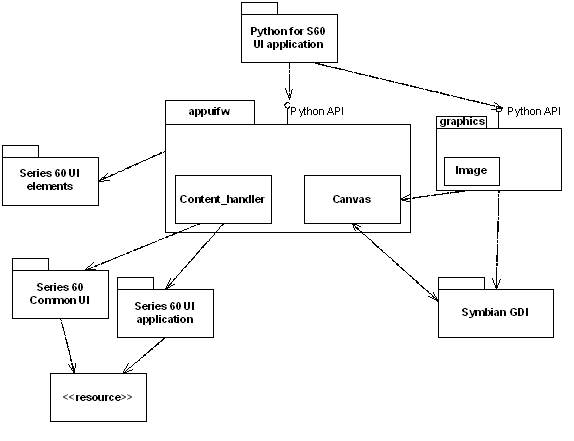
\includegraphics[width=\textwidth]{ui-overview}
\caption{Python for S60 UI environment overview}
\label{fig:ui-overview}
\end{figure}

\subsection{Basics of appuifw Module}
\label{subsec:basics}
Figure \ref{fig:normal-uilayout} shows the layout of a S60 application 
UI in the normal screen mode and a summary of how it relates to the services 
available at the \module{appuifw} API. For alternative layouts, see 
Figure \ref{fig:alternate-uilayouts}.

\begin{figure}
\centering
%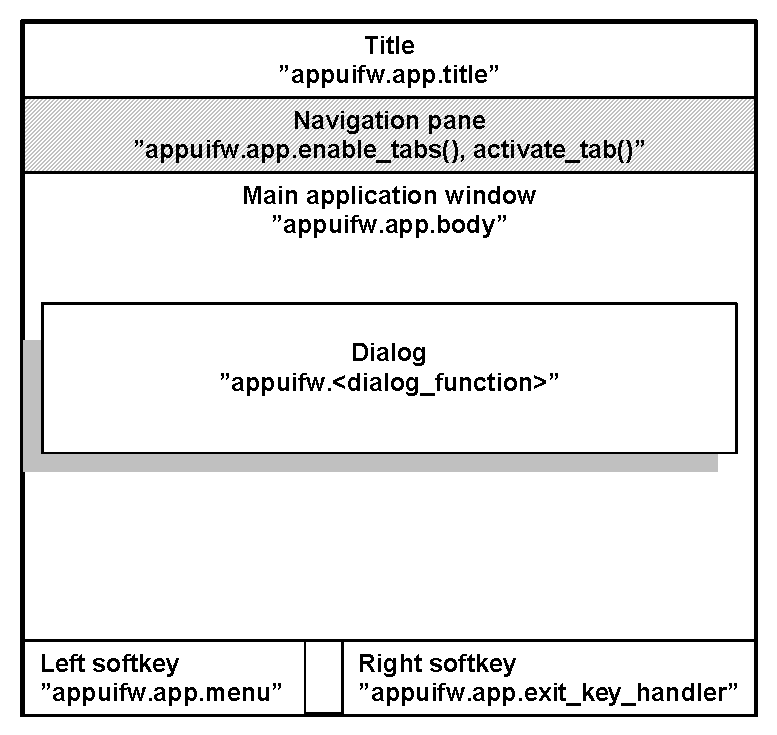
\includegraphics[width=0.7\textwidth]{screen-parts}
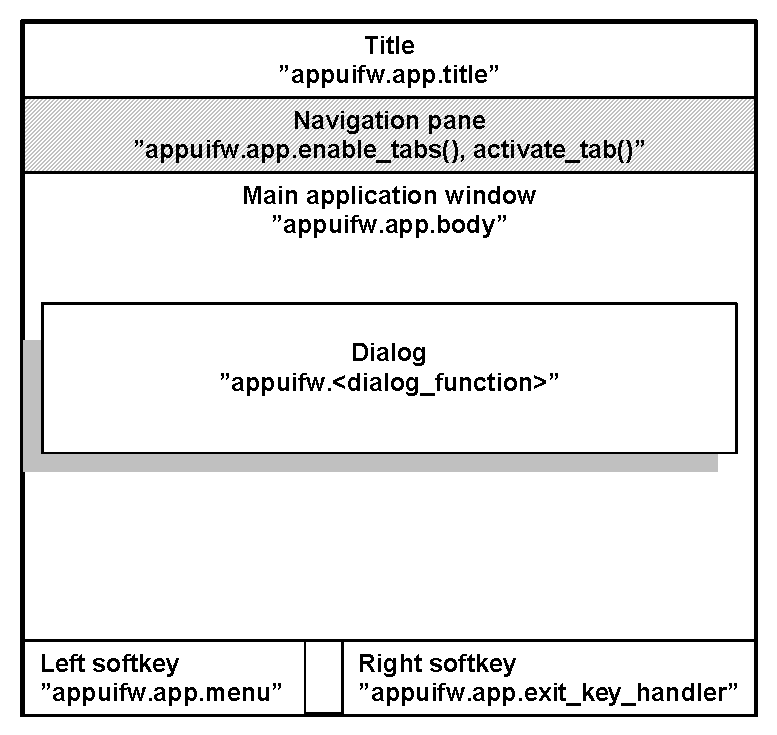
\includegraphics{screen-parts}
\caption{The different parts of the screen when using the 'normal' layout}
\label{fig:normal-uilayout}
\end{figure}

\begin{figure}
\centering
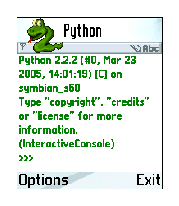
\includegraphics[width=\screenwidth]{layout-normal}
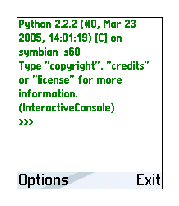
\includegraphics[width=\screenwidth]{layout-large}
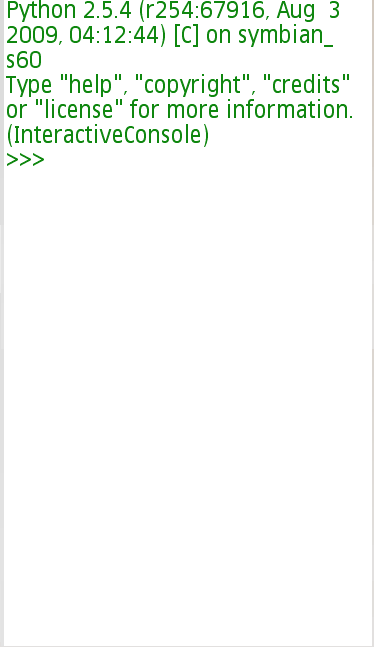
\includegraphics[width=\screenwidth]{layout-full}
\caption{UI layouts. left: 'normal', middle: 'large', right: 'full'}
\label{fig:alternate-uilayouts}
\end{figure}

The main application window may be set up to be occupied by a UI control.

A multi-view application can show the different views as tabs in the 
navigation pane and react as the users navigate between tabs. 

Dialogs always take precedence over the usual UI controls and appear on top 
of them.

UI controls are implemented as Python types. These types are available:

\begin{itemize}
\item \class{Text}
\item \class{Listbox}
\item \class{Canvas}
\end{itemize}
UI controls appear on the screen as soon as an instance of the corresponding 
Python type is set to the body field (\var{app.body}) of the current application UI.

\class{Form} is a versatile dialog implemented as a type.

The \class{Content_handler} type facilitates interfacing to other UI
applications and common high-level UI components. It is based on the
notion that designated handlers can reduce UI application interaction
to operations on MIME-type content.

The following dialogs are implemented as functions:

\begin{itemize}
\item \function{note}
\item \function{query}
\item \function{multi_query}
\item \function{selection_list}
\item \function{multi_selection_list}
\item \function{popup_menu}
\end{itemize}
A dialog becomes visible as soon as the corresponding Python function has 
been called. The function returns with the eventual user input or 
information on the cancellation of the dialog. \class{Form} is an 
exception; it is shown when its \method{execute} method is called.

\subsection{Softkeys}
\label{subsec:softkeys}
The softkeys are managed by the underlying S60 Platform. When no
dialog is visible, the right softkey is bound to application exit and
the left one represents an Options menu. Python for S60 offers
an interface for manipulating the menu and for binding the Exit key to
a Python-callable object (see Section \ref{subsec:application}). 

The native code that implements a dialog also manages the softkeys of the 
dialog, typically OK and Cancel. When the user input needs to be validated 
before accepting it and dismissing the dialog, it is best to use 
\class{Form}.

\subsection{Module Level Functions}
\label{subsec:module}
The following free functions - functions that do not belong to any class 
- are defined in the \module{appuifw} module:

\begin{funcdesc}{available_fonts}{}
Returns a list (Unicode) of all fonts available in the device.
\end{funcdesc}

\begin{funcdesc}{touch_enabled}{}
Returns 'True' if the device supports touch input, 'False' otherwise.
\end{funcdesc}

\begin{funcdesc}{query}{label, type\optional{, initial_value}}
Performs a query with a single-field dialog. The prompt is set to 
\var{label}, and the type of the dialog is defined by \var{type}. The 
value of \var{type} can be any of the following strings:

\begin{itemize}
\item \code{'text'}
\item \code{'code'}
\item \code{'number'}
\item \code{'date'}
\item \code{'time'}
\item \code{'query'}
\item \code{'float'}
\end{itemize}

The type of the optional \var{initial_value} parameter and the 
returned input depend on the value of \var{type}:

\begin{itemize}
\item For text fields, (\code{'text'}, \code{'code'}) it is Unicode
\item For number fields, it is numeric
\item For date fields, it is seconds since epoch rounded down to the nearest local midnight
\end{itemize}

A simple confirmation query and time query take no initial value and return 
\code{True/None} and seconds since local midnight, correspondingly. All 
queries return \code{None} if the users cancel the dialog. 

For \code{'float'} query the \var{initial_value} setting has no 
effect.
\end{funcdesc}


\begin{funcdesc}{multi_query}{label_1, label_2}
A two-field text (Unicode) input dialog. Returns the input values
as a 2-tuple. Returns \code{None} if the users cancel the dialog.
\end{funcdesc}

\begin{funcdesc}{note}{text\optional{, type\optional{, global}}}
Displays a note dialog of the chosen type with \var{text} 
(Unicode). The default value for \var{type} is \code{'info'}, which is 
automatically used if \var{type} is not set. \var{type} can be one of 
the following strings: \code{'error'}, \code{'info'} or 
\code{'conf'}. 

If \var{global} (integer) is any other value than zero a global note is 
displayed. A global note is displayed even if the Python application calling 
this function is in background. The same set of \var{type}s is supported as in 
standard note.
\end{funcdesc}

\begin{funcdesc}{popup_menu}{list\optional{, label}}
A pop-up menu style dialog. \var{list} representing the menu 
contents can be a list of Unicode strings or a list of Unicode string pairs 
(tuples). The resulting dialog list is then a single-style or a double-style 
list. A single-style list is shown in full; whereas a double-style list 
shows the items one at a time. Returns \code{None} if the user cancels the 
operation.
\end{funcdesc}

\begin{funcdesc}{selection_list}{choices\optional{, search_field=0}}
Executes a dialog that allows the users to select a list item and
returns the \var{index} of the chosen item, or \code{None} if the
selection is cancelled by the users. \var{choices} is a list of
Unicode strings.
\var{search_field} is \code{0} (disabled) by default and is optional. Setting it to \code{1} enables a search field (find pane) that facilitates searching for items in long lists. If enabled, the search field appears after you press a letter key.
\end{funcdesc}

\begin{funcdesc}{multi_selection_list}{choices\optional{, style='checkbox', search_field=0}}
  Executes a dialog that allows the users to select multiple list
  items.  Returns a tuple of indexes (a pair of Unicode strings) of
  the chosen items, or empty tuple if the no selection is made by
  the users. \var{choices} is a list of Unicode strings.  \var{style}
  is an optional string; the default value being \code{'checkbox'}.
  If \code{'checkbox'} is given, the list will be a checkbox list,
  where empty checkboxes indicate what items can be marked. The other
  possible value that can be set for \var{style} is
  \code{'checkmark'}. If \code{'checkmark'} is given, the list will be
  a markable list, which lists items but does not indicate
  specifically that items can be selected. To select items on a
  markable list, use the \var{'Options'} that has
  Mark/Unmark or the Edit key to select an item and the 
  Navigation key to browse the list. For example views on checkbox and
  markable lists, see
  \figurename~\ref{fig:checkbox-and-markable-list}.
  \var{search_field} is \code{0} (disabled) by default and is
  optional. Setting it to \code{1} enables a search field (find pane)
  that facilitates searching for items in long lists. If enabled, the
  search field is always visible with checkbox lists; with markable
  lists it appears by pressing a letter key.

Example:
\begin{verbatim}
tuple = appuifw.multi_selection_list([u'Harry', u'Ron', u'Hermione', u'Voldemort'], style='checkmark', search_field=1)
\end{verbatim}
\end{funcdesc}

\begin{figure}[htbp]
\centering
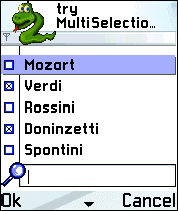
\includegraphics[width=\screenwidth]{checkbox-list}
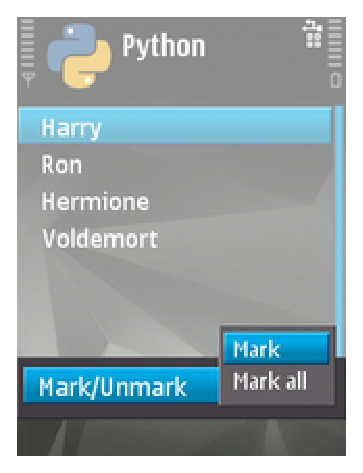
\includegraphics[width=\screenwidth]{markable-list}
\caption{Examples of a checkbox list (left) and a markable list (right)}
\label{fig:checkbox-and-markable-list}
\end{figure}

\subsection{Application Type}
\label{subsec:application}
A single implicit instance of this type always exists when \module{appuifw} 
module is present and can be referred to with the name \code{app}. New 
instances cannot be created by a Python program.

\begin{classdesc*}{Application}
Instances of \class{Application} type have the following attributes:

\begin{memberdesc}[Application]{body}
The UI control that is visible in the application's main window. Currently 
either \class{Text}, a \class{Listbox} object, \class{Canvas}, or 
\code{None}.
\end{memberdesc}

\begin{memberdesc}[Application]{directional_pad}
A boolean flag which controls the appearance of a virtual 4-way directional pad
that is displayed either at the bottom of the screen or on the right hand corner
depending on the orientation when using a Canvas. This is enabled by default on
devices that do not have a physical left and right soft key. This value is 
ignored on other devices, hence setting it to either True or False will have no effect.

Set it to \code{True} to enable 4-way directional pad and \code{False} to disable it.
\end{memberdesc}

\begin{memberdesc}[Application]{exit_key_handler}
A callable object that is called when the user presses the Exit softkey. 
Setting \member{exit_key_handler} to \code{None} sets it back to the 
default value.
\end{memberdesc}

\begin{memberdesc}[Application]{focus}
A callable object that is called with integer as parameter (0 = focus lost, 
1 = focus regained) when the application receives focus or it is switched to 
background. Focus is received e.g. when the application is switched from 
background to foreground or when the focus is regained from screensaver. 
Similarly when the screensaver is displayed, focus is lost.

Examples:
\begin{verbatim}
>>> import appuifw
>>> def cb(fg):
...   if(fg):
...     print "foreground"
...   else:
...     print "background"
...
>>> appuifw.app.focus=cb
>>> # switch to background, following text is printed from callback:
>>> background
>>> # switch to foreground, following text is printed from callback:
>>> foreground
\end{verbatim}

\begin{notice}
An improper callback can cause adverse effects. If you, for example,
define a callback which takes no parameters you will receive
never-ending \exception{TypeError} exceptions on the Nokia 6600.
\end{notice}

\end{memberdesc}

\begin{memberdesc}[Application]{menu}
This is a list of the following kinds of items:
\begin{itemize}
\item \code{(title, callback)} which creates a regular menu item
\item \code{(title, ((title, callback)\optional{...}))} which creates a submenu
\end{itemize}

\var{title} (Unicode) is the name of the item and \var{callback} the associated callable object. 
The maximum allowed number of items in a menu, or items in a submenu,
or submenus in a menu is 30.

Example:
\begin{verbatim}
appuifw.app.menu = [(u"Item 1", item1),
                    (u"Submenu 1", 
                        ((u"Subitem 1", subitem1),
                         (u"Subitem 2", subitem2)))]
\end{verbatim}
\end{memberdesc}

\begin{memberdesc}[Application]{orientation}
The orientation of the application. The orientation of the application can be 
one of the following values: \code{'automatic'} (this is the default value), 
\code{'portrait'} or \code{'landscape'}.
\end{memberdesc}

\begin{memberdesc}[Application]{screen}
The screen area used by an application. See \figurename~\ref{fig:alternate-uilayouts} for
example screens. The appearance of the application on the screen can
be affected by setting one of the following values: \code{'normal'},
\code{'large'} and \code{'full'}.

Examples:
\begin{verbatim}
appuifw.app.screen='normal'    # normal screen with title pane and softkey labels
appuifw.app.screen='large'     # only softkey labels visible
appuifw.app.screen='full'      # full screen mode on all devices
\end{verbatim}
\end{memberdesc}

\begin{memberdesc}[Application]{title}
The title of the application that is visible in the application's title
pane. Must be Unicode.
\end{memberdesc}

\begin{memberdesc}[Application]{track_allocations}
Set this to true if the interpreter should track all memory allocations and then
free the memory which was not explicitly released before application exit. The default
value of this attribute is true. As a consequence if there are any memory leaks in the
3rd party extension modules they will be released at the end. To check if there are
memory leaks(for debugging purposes) the following approach can be used :
\begin{verbatim}

appuifw.app.track_allocations = false

import my_extension
my_extension.do_something()

appuifw.app.track_allocations = true

\end{verbatim}
If the extension leaks memory then it will be reported at application exit.

\end{memberdesc}


Instances of \class{Application} type have the following methods:

\begin{methoddesc}[Application]{activate_tab}{index}
Activates the tab \var{index} counting from zero.
\end{methoddesc}

\begin{methoddesc}[Application]{full_name}{}
Returns the full name, in Unicode, of the native application in whose 
context the current Python interpreter session runs.
\end{methoddesc}

\begin{methoddesc}[Application]{layout}{layout_id}

Returns as a tuple the size and the position of the requested \code{layout_id}. 
The logical layouts are outlined partly in Figure \ref{fig:normal-uilayout}. The 
position is given from the top left corner. The \code{layout_id} can be one of 
the constants defined in module \module{appuifw}\footnote{Descriptions of the 
values are from the S60 SDK documentation \cite{S60Doc}.}:

\begin{datadesc}{EScreen} 
Screen.  
\end{datadesc}

\begin{datadesc}{EApplicationWindow} 
 Window that fills the entire screen.
\end{datadesc}

\begin{datadesc}{EStatusPane} 
Indicates common components for most of the applications.  
\end{datadesc}

\begin{datadesc}{EMainPane} 
The application main pane is used in all the applications.  
\end{datadesc}

\begin{datadesc}{EControlPane} 
Control pane.
\end{datadesc}

\begin{datadesc}{ESignalPane} 
The signal pane is used to indicate signal strength.  
\end{datadesc}

\begin{datadesc}{EContextPane} 
The context pane is used to indicate an active application.
\end{datadesc}

\begin{datadesc}{ETitlePane} 
Used to indicate the subject or the name of the main pane content. 
\end{datadesc}

\begin{datadesc}{EBatteryPane} 
The battery pane is used to indicate battery strength.  
\end{datadesc}

\begin{datadesc}{EUniversalIndicatorPane} 
The universal indicator pane is used to indicate items that require the user's 
attention while browsing applications. 
\end{datadesc}

\begin{datadesc}{ENaviPane} 
The navi pane is used to indicate navigation within an application, to provide 
context sensitive information to the user while entering or editing data, or to 
show additional information.  
\end{datadesc}

\begin{datadesc}{EFindPane} 
A fixed find pane is used with lists instead of the find pop-up window.  
\end{datadesc}

\begin{datadesc}{EWallpaperPane} 
Wallpaper pane.  
\end{datadesc}

\begin{datadesc}{EIndicatorPane} 
The universal indicator pane is used to indicate items that require the user's 
attention while browsing applications.  
\end{datadesc}

\begin{datadesc}{EAColumn} 
Used generally to display small sized graphics or heading texts.  
\end{datadesc}

\begin{datadesc}{EBColumn} 
Used generally to display large sized icons or heading texts.  
\end{datadesc}

\begin{datadesc}{ECColumn} 
Used generally to display data entered by the user. Overlaps with the D column. 
\end{datadesc}

\begin{datadesc}{EDColumn} 
Used generally to display additional icons. Overlaps with the C column. 
\end{datadesc}

\begin{datadesc}{EStaconTop} 
Top part of status and control panes in landscape layout.  
\end{datadesc}

\begin{datadesc}{EStaconBottom} 
Bottom part of status and control panes in landscape layout.  
\end{datadesc}

\begin{datadesc}{EStatusPaneBottom} 
Bottom part of status pane in landscape layout.  
\end{datadesc}

\begin{datadesc}{EControlPaneBottom} 
Bottom part of control pane in landscape layout.  
\end{datadesc}

\begin{datadesc}{EControlPaneTop} 
Top part of control pane in landscape layout.  
\end{datadesc}

\begin{datadesc}{EStatusPaneTop} 
Top part of status pane in landscape layout.
\end{datadesc}

Example:
\begin{verbatim}
>>> import appuifw
>>> appuifw.app.layout(appuifw.EMainPane)
((176, 144), (0, 44))
>>> # size and position (x, y) of the main pane in Nokia N70
\end{verbatim}

\end{methoddesc}

\begin{methoddesc}[Application]{set_exit}{}
Requests a graceful exit from the application as soon as the current script 
execution returns.
\end{methoddesc}

\begin{methoddesc}[Application]{set_tabs}{tab_texts\optional{,callback=None}}
Sets tabs with given names on them in the navigation bar; 
\var{tab_texts} is a list of Unicode strings. When the users 
navigate between tabs, \var{callback} gets called with the index 
of the active tab as an argument. Tabs can be disabled by giving an empty or 
one-item \var{tab_texts} list.
\end{methoddesc}

\begin{methoddesc}[Application]{uid}{}
Returns the UID, in Unicode, of the native application in whose 
context the current Python interpreter session runs.
\end{methoddesc}

\end{classdesc*}

\subsection{Form Type}
\label{subsec:form}
\class{Form} implements a dynamically configurable, editable multi-field 
dialog. \class{Form} caters for advanced dialog use cases with requirements 
such as free selectability of the combination of fields, possibility of 
validating the user input, and automatically producing the contents of some 
dialog fields before allowing the closing of the dialog. 

\begin{classdesc}{Form}{fields\optional{, flags=0}}
Creates a \class{Form} instance.
\var{fields} is a list of \emph{field descriptors}: \code{(label, type\optional{, value})} where

\var{label} is a Unicode string

\var{type} is one of the following strings: 
\code{'text'}, \code{'number'}, \code{'date'}, \code{'time'}, \code{'combo'}
or \code{'float'}

\var{value}, depending on \var{type}: Unicode string, numeric, float (seconds 
since Unix epoch rounded down to the nearest local midnight), float (seconds 
since local midnight), \code{([choice_label ...], index)} of float. For 
\code{'float'} \var{type} the initial value setting might not be shown in the 
UI.
\end{classdesc}

\class{Form} can also be configured and populated after construction. The 
configuration flags are visible as an attribute. \class{Form} implements 
the list protocol that can be used for setting the form fields, as well as 
obtaining their values after the dialog has been executed.

Instances of \class{Form} type have the following attributes:

\begin{memberdesc}[Form]{flags}
This attribute holds the values of the various configuration flags. 
Currently supported flags are:

\begin{datadesc}{FFormEditModeOnly}
When this flag is set, the form remains in edit mode while \method{execute} 
runs.
\end{datadesc}

\begin{datadesc}{FFormViewModeOnly}
When this flag is set, the form cannot be edited at all.
\end{datadesc}

\begin{datadesc}{FFormAutoLabelEdit}
This flag enables support for allowing the end-users to edit the labels of 
the form fields.
\end{datadesc}

\begin{datadesc}{FFormAutoFormEdit}
This flag enables automatic support for allowing the end-users to add and 
delete the form fields. Note that this is an experimental feature and is not 
guaranteed to work with all SDK versions.
\end{datadesc}

\begin{datadesc}{FFormDoubleSpaced}
When this flag is set, double-spaced layout is applied when the form is 
executed: one field takes two lines, as the label and the value field are on 
different lines.
\end{datadesc}
\end{memberdesc}

\begin{memberdesc}[Form]{menu}
A list of \code{(title, callback)} pairs, where 
each pair describes an item in the form's menu bar that is active while the 
dialog is being executed. \var{title} (Unicode) is the name of 
the item and \var{callback} the associated callable object.
\end{memberdesc}

\begin{memberdesc}[Form]{save_hook}
This attribute can be set to a callable object that receives one argument 
and returns a Boolean value. It gets called every time the users want to 
save the contents of an executing \class{Form} dialog. A candidate list for 
new form content - a list representing the currently visible state of the 
UI - is given as an argument. The list can be modified by 
\member{save_hook}. If \member{save_hook} returns \code{True}, the 
candidate list is set as the new contents of the form. Otherwise, the form 
UI is reset to reflect the field list contained in \class{Form} object.
\end{memberdesc}

Instances of \class{Form} type have the following methods:

\begin{methoddesc}[Form]{execute}{}
Executes the dialog by making it visible on the UI.
\end{methoddesc}

\begin{methoddesc}[Form]{insert}{index, field_descriptor}
Inserts the field descriptor into the \class{Form} before the given \var{index}.
\end{methoddesc}

\begin{methoddesc}[Form]{pop}{}
Removes the last field descriptor from the \class{Form} and returns it.
\end{methoddesc}

\begin{methoddesc}[Form]{length}{}the number of field descriptors in the form.
\end{methoddesc}

The subscript notation \code{f[i]} can be used to access or modify the
i-th element of the form \code{f}. Same limitations as discussed above
in the context of the flag \constant{FFormAutoFormEdit} apply to
modifying a form while it is executing. The ability to change the
schema of a form while it is executing is an experimental feature.

\subsection{Text Type}
\label{subsec:mylabel5}
\class{Text} is a text editor UI control. For examples on the options 
available with \class{Text}, see Figure \ref{fig:text-styles}.

\begin{figure}[htbp]
\centering
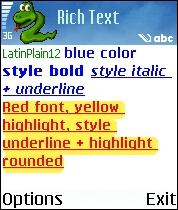
\includegraphics[width=\screenwidth]{text-styles-1}
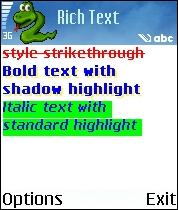
\includegraphics[width=\screenwidth]{text-styles-2}
\caption{Examples of the options available for Text type}
\label{fig:text-styles}
\end{figure}

Instances of \class{Text} type have the following attributes:

\begin{memberdesc}[Text]{color}
The color of the text. \code{color} supports the same color representation 
models as the \module{graphics} module. For the supported color 
representation models, see Section \ref{sec:graphics}.
\end{memberdesc}

\begin{memberdesc}[Text]{focus}
A Boolean attribute that indicates the focus state of the control. Editor 
control also takes the ownership of the navigation bar, and this feature is 
needed to enable the usage of this control in applications that use the 
navigation bar - for example, navigation tabs.
\end{memberdesc}

\begin{memberdesc}[Text]{font} 
The font of the text. There are two possible ways to set this attribute:

\begin{itemize}

\item Using a supported Unicode font, for example \code{u"Latin12"}. Trying to set a font which is not supported by the device has no effect. A list of supported fonts can be retrieved by using \function{appuifw.available_fonts}.

Example, setting font:
\begin{verbatim}
t = appuifw.Text()
t.font = u"albi17b" # sets font to Albi 17 bold
t.font = u"LatinPlain12" # sets font to Latin Plain 12
\end{verbatim}
\item Using one of the default device fonts that are associated with the following labels (plain strings):
\code{'annotation', 'title', 'legend', 'symbol', 'dense', 'normal'.}

Example, setting font: 
\begin{verbatim}
t.font = "title" # sets font to the one used in titles
\end{verbatim}

Example, checking the currently set font: 
\begin{verbatim}
unicodeFont = t.font
\end{verbatim}
\end{itemize}

The attribute value retrieved is always a Unicode string. If the font has 
been set with a label, for example, \code{'title'}, the attribute will 
retrieve the font associated with that label. 
\end{memberdesc}

\begin{memberdesc}[Text]{highlight_color}
The highlight color of the text. \code{highlight_color} supports the 
same color representation models as the \module{graphics} module. For the 
supported color representation models, see Section \ref{sec:graphics}.
\end{memberdesc}

\begin{memberdesc}[Text]{style}
The style of the text. The flags for this attribute are defined in the 
\module{appuifw} module. These flags can be combined by using the binary 
operator \code{|}. The flags can be divided into two types: text style 
and text highlight. Text style flags can be freely combined with each other. 
However, one or more text style flags can be combined with only one text 
highlight flag. The flags are:

Text style:

\begin{datadesc}{STYLE_BOLD} 
Enables bold text.
\end{datadesc}

\begin{datadesc}{STYLE_UNDERLINE}
Enables underlined text.
\end{datadesc}

\begin{datadesc}{STYLE_ITALIC} 
Enables italic text.
\end{datadesc}

\begin{datadesc}{STYLE_STRIKETHROUGH } 
Enables strikethrough.
\end{datadesc}

Text highlight:

\begin{datadesc}{HIGHLIGHT_STANDARD}
Enables standard highlight.
\end{datadesc}

\begin{datadesc}{HIGHLIGHT_ROUNDED}
Enables rounded highlight.
\end{datadesc}

\begin{datadesc}{HIGHLIGHT_SHADOW}
Enables shadow highlight.
\end{datadesc}

Only one highlight is allowed to be used at once. Therefore, it is possible 
to combine only one highlight with one or more text styles.

Examples:
\begin{verbatim}
t = appuifw.Text()

# These and other similar values and combinations are valid:
t.style = appuifw.STYLE_BOLD
t.style = appuifw.STYLE_UNDERLINE
t.style = appuifw.STYLE_ITALIC
t.style = appuifw.STYLE_STRIKETHROUGH
t.style = (appuifw.STYLE_BOLD|
	   appuifw.STYLE_ITALIC|
	   appuifw.STYLE_UNDERLINE)

# These values are valid:
t.style = appuifw.HIGHLIGHT_STANDARD
t.style = appuifw.HIGHLIGHT_ROUNDED
t.style = appuifw.HIGHLIGHT_SHADOW

# This combination is NOT valid:
# Invalid code, do not try!
t.style = (appuifw.HIGHLIGHT_SHADOW|appuifw.HIGHLIGHT_ROUNDED)
\end{verbatim}
\end{memberdesc}

Instances of \class{Text} type have the following methods:

\begin{methoddesc}[Text]{add}{text}
Inserts the Unicode string \var{text} to the current cursor position.
\end{methoddesc}

\begin{methoddesc}[Text]{bind}{event_code, callback}
Binds the callable Python object \var{callback} to event
\var{event_code}. The key codes are defined in 
the \module{key_codes} library module. The call 
\code{bind(event_code, None)} clears an 
existing binding. In the current implementation the event is always
passed also to the underlying native UI control.
\end{methoddesc}

\begin{methoddesc}[Text]{clear}{}
Clears the editor.
\end{methoddesc}

\begin{methoddesc}[Text]{delete}{\optional{pos=0, length=len()}}
Deletes \var{length} characters of the text held by the editor control, 
starting from the position \var{pos}.
\end{methoddesc}

\begin{methoddesc}[Text]{get_pos}{}
Returns the current cursor position.
\end{methoddesc}

\begin{methoddesc}[Text]{len}{}
Returns the length of the text string held by the editor control.
\end{methoddesc}

\begin{methoddesc}[Text]{get}{\optional{pos=0, length=len()}}
Retrieves \code{length} characters of the text held by the editor control, 
starting from the position \var{pos}.
\end{methoddesc}

\begin{methoddesc}[Text]{set}{text}
Sets the text content of the editor control to Unicode string 
\var{text}.
\end{methoddesc}

\begin{methoddesc}[Text]{set_pos}{cursor_pos}
Sets the cursor to \var{cursor_pos}.
\end{methoddesc}

\subsection{Listbox Type}
\label{subsec:listbox}

\begin{figure}[htbp]
\centering
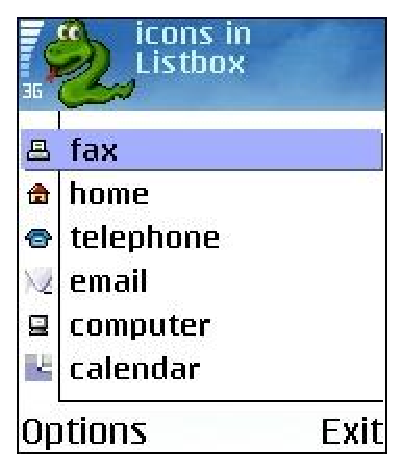
\includegraphics[width=\screenwidth]{listbox-with-icons}
\caption{Listbox with icons}
\label{fig:listbox-with-icons}
\end{figure}

An instance of this UI control type is visible as a listbox, also known as a 
list in Symbian, that can be configured to be a single-line item or a 
double-item listbox. Figure \ref{fig:listbox-with-icons} shows a single-line 
item Listbox with icons. For more information on the MBM and MIF formats, 
see Section \ref{subsec:icon}.

\begin{classdesc}{Listbox}{list, callback}
Creates a \class{Listbox} instance. A callable object 
\var{callback} gets called when a listbox selection has been 
made. \code{list} defines the content of the listbox and can be one of the 
following:

\begin{itemize}
\item A normal (single-line item) listbox: a list of Unicode strings, for example \code{[unicode_string item1, unicode_string item2]}
\item A double-item listbox: a two-element tuple of Unicode strings , for example \code{[(unicode_string item1, unicode_string item1description), (unicode_string item2, unicode_string item2description)]}
\item A normal (single-line item) listbox with graphics: a two-element tuple consisting of a Unicode string and an \class{Icon} object, for example \code{[(unicode_string item1, icon1), (unicode_string item2, icon2)]}.
\item A double-item listbox with graphics: a three-element tuple consisting of two Unicode strings and one \class{Icon} object, for example \code{[(unicode_string item1, unicode_string item1description, icon1), (unicode_string item2, unicode_string item2description, icon2)]}
\end{itemize}

Example: To produce a normal (single-line item) listbox with graphics:
\begin{verbatim}
icon1 = appuifw.Icon(u"z:\\resource\\apps\\avkon2.mbm", 28, 29)
icon2 = appuifw.Icon(u"z:\\resource\\apps\\avkon2.mbm", 40, 41)
entries = [(u"Signal", icon1),
           (u"Battery", icon2)]
lb = appuifw.Listbox(entries, lbox_observe)
\end{verbatim}
\end{classdesc}

\begin{notice}[note]
Known issue: Using this widget in large/full screen mode results in an unrefreshed area at the bottom of the screen.
\end{notice}

Instances of \class{Listbox} type have the following methods and properties:

\begin{methoddesc}[Listbox]{bind}{event_code, callback}
Binds the callable Python object \var{callback} to event 
\var{event_code}. The key codes are defined in 
the \module{key_codes} library module. The call
\code{bind(event_code, None)} clears an 
existing binding. In the current implementation the event is always passed 
also to the underlying native UI control.
\end{methoddesc}

\begin{methoddesc}[Listbox]{current}{}
Returns the currently selected item's index in the \class{Listbox}.
\end{methoddesc}

\begin{methoddesc}[Listbox]{set_list}{list\optional{, current}}
Sets the \class{Listbox} content to a list of Unicode strings or a
list of tuples of Unicode strings. The accepted structures of \var{list} are the
same as in the \class{Listbox} constructor. The optional argument \var{current} is the index of the focused list item.
\end{methoddesc}

\begin{memberdesc}[Listbox]{size}
The size of the \class{Listbox} as a tuple (width, height) - Read only.
\end{memberdesc}

\begin{memberdesc}[Listbox]{position}
The coordinates (as a tuple) of the top left corner of the \class{Listbox} -
Read only.
\end{memberdesc}

\subsection{Icon Type}
\label{subsec:icon}
An instance of \class{Icon} type encapsulates an icon to be used together 
with a \class{Listbox} instance. Note that currently \class{Icon} can only 
be used with \class{Listbox} (see Section \ref{subsec:listbox}).

MBM is the native Symbian OS format used for pictures. It is a
compressed file format where the files can contain several bitmaps and
can be referred to by a number. An \code{.mbg} file is the header file
usually associated with an \code{.mbm} file, which includes symbolic
definitions for each bitmap in the file. For example, an
\file{avkon.mbm} file has an associated index file called
\file{avkon.mbg}, which is included in S60 SDKs. For more information
on the MBM format and the bitmap converter tool, see \cite{S60Doc} and
search the topics with the key term "How to provide Icons"; this topic
also points you to the Bitmap Converter tool that can be used for
converting bitmaps into the MBM format.

\begin{classdesc}{Icon}{filename, bitmap, bitmapMask}
Creates an icon. \var{filename} is a Unicode file name and must 
include the whole path. Note that MBM is the only file formats supported.
\var{bitmap} and \var{bitmapMask} are integers that represent the index of 
the icon and icon mask inside that file respectively.
\end{classdesc}

Example: The following builds an icon with the standard signal symbol:
\begin{verbatim}
icon = appuifw.Icon(u"z:\\resource\\apps\\avkon2.mbm", 28, 29)
\end{verbatim}

\subsection{Content\_handler Type}
\label{subsec:content}

An instance of \class{Content_handler} handles data content by its MIME 
type.

\begin{classdesc}{Content_handler}{\optional{callback}}
Creates a \class{Content_handler} instance. A Content_handler handles
data content by its MIME type. The optional
\var{callback} is called when the embedded handler application 
started with the \method{open} method finishes. 
\end{classdesc}

Instances of \class{Content_handler} type have the following methods:

\begin{methoddesc}[Content_handler]{open}{filename}
Opens the file \var{filename} (Unicode) in its handler 
application if one has been registered for the particular MIME type. The 
handler application is embedded in the caller's thread. The call to this 
function returns immediately. When the handler application finishes, the 
\var{callback} that was given to the \class{Content_handler} 
constructor is called.
\end{methoddesc}

\begin{methoddesc}[Content_handler]{open_standalone}{filename}
Opens the file \var{filename} (Unicode) in its handler 
application if one has been registered for the particular MIME type. The 
handler application is started in its own process. The call to this function 
returns immediately. Note that \var{callback} is not called for 
applications started with this method.
\end{methoddesc}

\subsection{Canvas Type}
\label{subsec:canvas}
\class{Canvas} is a UI control that provides a drawable area on the screen 
and support for handling raw key events. \class{Canvas} supports the 
standard drawing methods that are documented in Section \ref{sec:graphics}.

\begin{classdesc}{Canvas}{\optional{redraw_callback=None, event_callback=None,
                                  resize_callback=None}}
Constructs a \class{Canvas}. The optional parameters are callbacks
that are called when specific events occur. 

\note{Watch out for cyclic
references here. For example, if the callbacks are methods of an
object that holds a reference to the \class{Canvas}, a reference cycle
is formed that must be broken at cleanup time or the
\class{Canvas} will not be freed.}

\var{redraw_callback} is called whenever a part of the \class{Canvas} 
has been obscured by something, is then revealed, and needs to be
redrawn. This can typically happen, for example, when the user
switches away from the Python application and back again, or after
displaying a pop-up menu. The callback takes as its argument a
four-element tuple that contains the top-left and the bottom-right
corner of the area that needs to be redrawn. In many cases redrawing
the whole
\class{Canvas} is a reasonable option. 

\var{event_callback} is called whenever a raw key event is received or when a 
pointer event occurs(only on touch input supported devices).
There are three kinds of key events: \code{EEventKeyDown},
\code{EEventKey}, and \code{EEventKeyUp}. When a user presses a key 
down, events \code{EEventKeyDown} and \code{EEventKey} are generated. 
When the key is released, an \code{EEventKeyUp} event is generated.

Pointer events are generated by touch input supported devices. When the screen
is touched the \code{EButton1Down} event is generated, \code{EDrag} while the
finger/stylus is dragged across the screen and then \code{EButton1Up} when the
finger/stylus is lifted.

The argument to the \var{event_callback} is a dictionary that contains 
the following data:

For key events:
\begin{itemize}
\item \code{'type'}: one of \code{EEventKeyDown}, \code{EEventKey}, or 
\code{EEventKeyUp}
\item \code{'keycode'}: the keycode of the key
\item \code{'scancode'}: the scancode of the key
\item \code{'modifiers'}: the modifiers that apply to this key event
\end{itemize}

For pointer events:
\begin{itemize}
\item \code{'type'}: one of the several pointer events - \code{EButton1Up}, 
\code{EButton1Down}, \code{EDrag} etc..
\item \code{'modifiers'}: the modifiers that apply to this pointer event
\item \code{'pos'}: A tuple containing the x-y pointer co-ordinates
\end{itemize}

Each key on the keyboard has one or more scancodes and zero or more keycodes 
associated with it. A scancode represents the physical key itself and a 
keycode is the result of state-related operating system defined processing 
done on the key. For keys that correspond to a symbol in the current 
character set of the phone, the keycode is equal to the code of the 
corresponding symbol in that character set. For example, if you are using 
the Nokia Wireless Keyboard (SU-8W), pressing the key A will always produce 
the scancode 65 (ASCII code for an upper case A), but the keycode 
could be either 65 or 91 (ASCII code for a lower case A) depending on 
whether or not the Shift key is pressed or Caps Lock is active. 

The \module{key_codes} module contains definitions for the keycodes and 
scancodes. See \figurename~\ref{fig:keyboard} for the codes of the most 
common keys on the phone keypad. 

Some keys are handled in a special way:

\begin{itemize}
\item A short press of the Edit key causes it to stay down, meaning that no \code{EEventKeyUp} event is sent. The event is only sent after a long press.
\item Detecting presses of the Voice tags key or the Power key is not supported.
\item If the right softkey is pressed, the \code{appuifw.app.exit_key_handler} callback is always executed.
\end{itemize}

There is no way to prevent the standard action of the Hang-up key, the Menu 
key, the Power key or the Voice tags key from taking place.

\begin{figure}
\centering
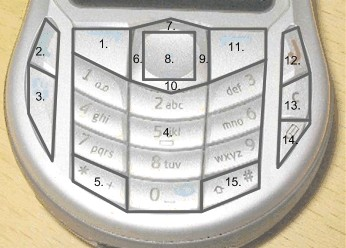
\includegraphics[width=5in]{6630keyboard}
%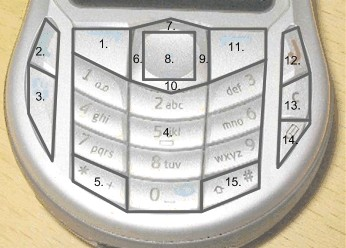
\includegraphics[width=3.60in,height=2.58in]{6630keyboard}
%\centerline{\includegraphics[width=3.60in,height=2.58in]{API_Reference_for_Python11.eps}} \par & 
\begin{tableiii}{lll}{textrm}{Key}{Keycode}{Scancode}
\lineiii{1.}{EKeyLeftSoftkey}{EScancodeLeftSoftkey}
\lineiii{2.}{EKeyYes}{EScancodeYes}
\lineiii{3.}{EKeyMenu}{EScancodeMenu}
\lineiii{4.}{EKey0...9}{EScancode0...9}
\lineiii{5.}{EKeyStar}{EScancodeStar}
\lineiii{6.}{EKeyLeftArrow}{EScancodeLeftArrow}
\lineiii{7.}{EKeyUpArrow}{EScancodeUpArrow}
\lineiii{8.}{EKeySelect}{EScancodeSelect}
\lineiii{9.}{EKeyRightArrow}{EScancodeRightArrow}
\lineiii{10.}{EKeyDownArrow}{EScancodeDownArrow}
\lineiii{11.}{EKeyRightSoftkey}{EScancodeRightSoftkey}
\lineiii{12.}{EKeyNo}{EScancodeNo}
\lineiii{13.}{EKeyBackspace}{EScancodeBackspace}
\lineiii{14.}{EKeyEdit}{EScancodeEdit}
\lineiii{15.}{EKeyHash}{EScancodeHash}
\end{tableiii}
\caption{Keycodes and scancodes for phone keys usable from Python applications}
\label{fig:keyboard}
\end{figure}

\var{resize_callback} is called when screen size is changed when the 
\class{Canvas} rect size has been changed. The callback takes as its argument a
two-element tuple that contains the new clientRect width and height. 

\end{classdesc}

Instances of \class{Canvas} type have the following methods:

\begin{methoddesc}[Canvas]{bind}{pointer_event, callable\optional{, ((x1, y1), (x2, y2))}}
This method can be used to listen to specific pointer events. The
\var{pointer_event} argument can be any one of the pointer events listed in the
\module{key_codes} module.

The most common pointer events are:

\begin{itemize}
\item \code{EButton1Down} - Pen down event 
\item \code{EButton1Up}   - Pen up event
\item \code{EDrag}        - Drag event (This event is only received when button1 is down)
\item \code{ESwitchOn}    - Switch on event caused by a screen tap.
\end{itemize}

\var{callable} is called when the pointer_event and the co-ordinate 
(if specified) criterion matches.

\var{((x1, y1), (x2, y2))} is an optional argument that can be passed to
specify the screen area to monitor for any specific pointer event. The two
co-ordinate tuple corresponds to the top-left and bottom-right points. This
argument will be ignored if the event is not a pointer event.

There are several ways in which bind can be used:

\begin{itemize}
\item \code{my_canv.bind(EButton1Up, callback)} - The callback is called when
EButton1Up event is generated anywhere in the canvas.

\item \code{my_canv.bind(EButton1Up, green_callback, ((x1, y1), (x2, y2)))} - The 
callback is called when the EButton1Up pointer event occurs inside the screen
area specified.

\item \code{my_canv.bind(EButton1Up, yellow_callback, ((x3, y3), (x4, y4)))} - 
Registers another callback for a different region but for the same pointer
event. When two screen areas overlap, the callback registered last will be
called when pointer events occur in the intersected region. 

\item \code{my_canv.bind(EButton1Up, callback3, ((x1, y1), (x2, y2)))} - If the
pointer event and the screen area to be monitored are the same, the callback
passed will replace the old callback already registered. 

\item \code{my_canv.bind(EButton1Up, None, ((x1, y1), (x2, y2)))} - If the pointer
event and the screen area to be monitored are the same, and the callback passed
is None, the callback registered previously is cleared.

\item \code{my_canv.bind(EButton1Up, None)} - All callbacks previously registered
for this pointer event are cleared, regardless of whether it was for a specific
screen area or for the entire canvas.
\end{itemize}

\begin{figure}
\centering
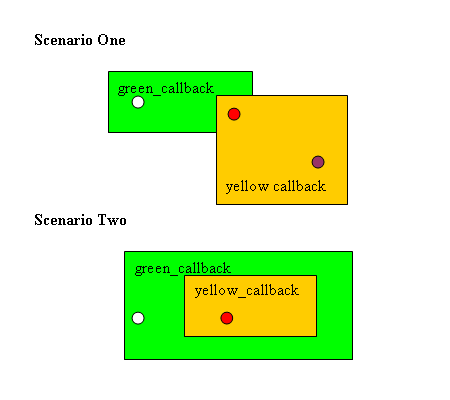
\includegraphics[width=5in]{bind-scenarios}
\caption{Canvas bind scenarios}
\label{fig:bind-scenarios}
\end{figure}

Clicking on the white spot should result in \code{green_callback} to be called. 
Clicking on the red spot should result in \code{yellow_callback} to be called in both
the scenarios shown above provided the \code{yellow_callback} was registered last. 
Clicking on the purple spot should result in \code{yellow_callback} to be called.

\end{methoddesc}

\begin{methoddesc}[Canvas]{begin_redraw}{\optional{((x1, y1), (x2, y2))}}
This is an explicit function that can be used to signal the window server that 
"I'm about to redraw this area". This method tells the window server that the 
window is about to respond to the last redraw event by redrawing the specified 
rectangle. This causes the window server to clear the rectangle, and remove it 
from the invalid region.
The optional co-ordinates x1, y1, x2, y2 should be the rectangle that has to be marked
for redrawing.

After the redraw is complete the application should call end_redraw().

\note{The begin_redraw and end_redraw methods should not be called inside the
redraw callback function.}

Couple of FAQs on redraw/non-redraw drawing:

Question: What is non-redraw drawing?
\begin{itemize}
\item "Non-redraw drawing" is any canvas/graphics drawing operation performed 
outside of begin_redraw()/end_redraw().
\end{itemize}

Question: What should applications do instead of non-redraw drawing?
\begin{itemize}
\item "Redraw drawing" is any drawing delimited by begin_redraw()/end_redraw().
\end{itemize}

Question: Why is non-redraw drawing bad for performance?
\begin{itemize}
\item The window server caches drawing operations in the redraw store.
Delimiting drawing with begin_redraw()/end_redraw() allows window server to 
efficiently manage drawing operations. 

If applications perform drawing operations outside begin_redraw/end_redraw,
window server cannot cull drawing operations from its cache of drawing 
operations, because it cannot know whether a set of drawing operations has 
been superceded by a new set.
In this scenario every frame of drawing that is done on a non-redraw drawing window 
will become slower and slower as it draws all the drawing operations for the 
entire history of the window (well actually up until the last begin_redraw/end_redraw 
for the whole window).

If an application performs begin_redraw/end_redraw, it tells the window server 
that it can throw away any old drawing operations it had for the area of the 
window specified in the redraw, thus allowing for more optimal management of 
drawing operations.
\end{itemize}

Question: What are the changes required for redraw drawing?
\begin{itemize}
\item Applications should delimit their drawing with begin_redraw()/end_redraw() 
- i.e. they should replace non-redraw drawing with redraw drawing. Sometimes, 
this is as straight forward as adding these calls to existing rendering code.
In other cases (where the application has been drawing using "incremental updates" 
to the window, the application drawing code would need to be reworked to perform a 
full refresh of the area redrawn for the rect provided in begin_redraw(rect).
\end{itemize}
\end{methoddesc}

\begin{methoddesc}[Canvas]{end_redraw}{}
Ends the current redraw. This function should be called when redrawing is complete.
\end{methoddesc}


Instances of \class{Canvas} type have the following attribute:

\begin{memberdesc}[Canvas]{size}
A two-element tuple that contains the current width and height of the 
\class{Canvas} as integers.
\end{memberdesc}

Instances of \class{Canvas} type have the same standard drawing methods 
that are documented in Section \ref{sec:graphics}.

\subsection{InfoPopup Type}
\label{subsec:infopopup}

An instance of \class{InfoPopup} type encapsulates an UI tip widget. This widget 
can be placed on top of other widgets to provide e.g. usage information to the 
user. The widget disappears as soon as the device's user presses any key or when 
the timer behind the \class{InfoPopup} is triggered.

\begin{classdesc}{InfoPopup}{}
Creates an \class{InfoPopup}.
\end{classdesc}

\begin{methoddesc}[InfoPopup]{show}{text, \optional{(x_coord, y_coord), 
time_shown, time_before, alignment}}
Show \var{text} (Unicode) in the \class{InfoPopup}. The optional parameters are 
the location (a tuple from the upper left corner), the time the popup is 
visible, \var{time_shown} (in milliseconds), the time before the popup, 
\var{time_before} (in milliseconds) and the alignment of the popup.

The default values are: the coordinates \code{(0, 0)}, \var{time_shown} 5 
seconds, \var{time_before} 0 seconds and for the alignment 
\code{appuifw.EHLeftVTop}.

The \var{alignment} can be one of the constants defined in module 
\code{appuifw}\footnote{Descriptions of the values are from the S60 SDK 
documentation \cite{S60Doc}.}:

\begin{datadesc}{EHLeftVTop} 
Object is left and top aligned. 
\end{datadesc}

\begin{datadesc}{EHLeftVCenter} 
Object is left aligned and centred vertically. 
\end{datadesc}

\begin{datadesc}{EHLeftVBottom} 
Object is left aligned and at the bottom. 
\end{datadesc}

\begin{datadesc}{EHCenterVTop} 
Object is centre aligned horizontally and at the top. 
\end{datadesc}

\begin{datadesc}{EHCenterVCenter} 
Object is centred horizontally and vertically. 
\end{datadesc}

\begin{datadesc}{EHCenterVBottom} 
Object is centred horizontally and at the bottom. 
\end{datadesc}

\begin{datadesc}{EHRightVTop} 
Object is right and top aligned. 
\end{datadesc}
 
\begin{datadesc}{EHRightVCenter} 
Object is right aligned and centred vertically. 
\end{datadesc}

\begin{datadesc}{EHRightVBottom} 
Object is right aligned and at the bottom. 
\end{datadesc}

\end{methoddesc}

\begin{methoddesc}[InfoPopup]{hide}{}
Hides the popup immediately.
\end{methoddesc}

Example:

\begin{verbatim}
>>> import appuifw
>>> i=appuifw.InfoPopup()
>>> i.show(u"Here is the tip.", (0, 0), 5000, 0, appuifw.EHRightVCenter)
>>>
\end{verbatim}

% Copyright (c) 2008-2009 Nokia Corporation
%
% Licensed under the Apache License, Version 2.0 (the "License");
% you may not use this file except in compliance with the License.
% You may obtain a copy of the License at
%
%     http://www.apache.org/licenses/LICENSE-2.0
%
% Unless required by applicable law or agreed to in writing, software
% distributed under the License is distributed on an "AS IS" BASIS,
% WITHOUT WARRANTIES OR CONDITIONS OF ANY KIND, either express or implied.
% See the License for the specific language governing permissions and
% limitations under the License.

\section{\module{globalui} --- 
    Interface to the S60 global UI notifiers }
\label{sec:globalui}

\declaremodule{extension}{globalui}
\platform{S60}
\modulesynopsis{Interface to the S60 global UI notifiers.}

The \module{globalui} module offers an interface to the S60 global UI notifiers. 
This allows a global note and query to be launched from an application which does not 
have a UI environment. 
The \module{globalui} module have functions:

\begin{funcdesc}{global_note}{note_text\optional{, type}}
Displays a note of the chosen type with \var{note_text} 
(Unicode). The default value for \var{type} is \code{'info'}. \var{type} can be 
one of the following strings: \code{'error'}, \code{'text'}, \code{'warn'}, \code{'charging'},
\code{'wait'}, \code{'perm'},\code{'not_charging'}, \code{'battery_full'}, \code{'battery_low'}, 
\code{'recharge_battery'}, or \code{'confirm'}. 
\end{funcdesc}

\begin{funcdesc}{global_query}{query_text\optional{, timeout}}
Displays a global confirmation query with \var{query_text} (Unicode). Returns 
\code{1} when the user presses 'Yes' and \code{0} otherwise. If the user does 
not respond to the query within \var{timeout} seconds, returns \code{None}. 
If the \var{timeout} value is 0, then the query waits indefinitely for user input. 
The default value for \var{timeout} is 0. The \var{timeout} value should be an integer.
\end{funcdesc}

\begin{funcdesc}{global_msg_query}{query_text, header_text\optional{, timeout}}
Displays a global message query with \var{query_text}(Unicode). \var{header_text} is used 
to set the heading string of the query. Returns \code{1} when the user 
presses 'OK' and \code{0} otherwise. If the user does not respond to the query within 
\var{timeout} seconds, returns \code{None}. If the \var{timeout} value is \code{0}, then the query 
waits indefinitely for user input. The default value for \var{timeout} is \code{0}. 
The \var{timeout} value should be an integer.
\end{funcdesc}

\begin{funcdesc}{global_popup_menu}{option_items\optional{, header_text, timeout}} 
Displays a global menu with \var{option_items}(Unicode). \var{header_text} is used to set the 
heading string of the menu. If no value is passed for \var{header_text}, then the header will
not be displayed. Returns the index value of the selected item from the list. If the user does
not respond to the menu within \var{timeout} seconds, returns \code{None}. If the \var{timeout}
value is \code{0}, then the menu waits indefinitely for the input. The default value for \var{timeout} 
is \code{0}. The \var{timeout} value should be an integer.
\end{funcdesc}

Example:
\begin{verbatim}
>>> import globalui, time
...
>>> text_to_show = u"text for showing note"
>>> globalui.global_note(text_to_show,'error')
>>> time.sleep(6)
>>> globalui.global_note(text_to_show)
>>> time.sleep(6)
>>> result = globalui.global_query(u"do you want to continue ?")
>>> time.sleep(6)
>>> listresult = globalui.global_popup_menu([u"MenuItem1", u"MenuItem2"],u"Select item",5)
...   
\end{verbatim}

% Copyright (c) 2005-2009 Nokia Corporation
%
% Licensed under the Apache License, Version 2.0 (the "License");
% you may not use this file except in compliance with the License.
% You may obtain a copy of the License at
%
%     http://www.apache.org/licenses/LICENSE-2.0
%
% Unless required by applicable law or agreed to in writing, software
% distributed under the License is distributed on an "AS IS" BASIS,
% WITHOUT WARRANTIES OR CONDITIONS OF ANY KIND, either express or implied.
% See the License for the specific language governing permissions and
% limitations under the License.

\section{\module{graphics} ---
  A graphics related services package}
\label{sec:graphics}

\declaremodule{extension}{graphics}
\platform{S60}
\modulesynopsis{A graphics related services package.}

The \module{graphics} module provides access to the graphics primitives and 
image loading, saving, resizing, and transformation capabilities provided by 
the Symbian OS. 

The module is usable from both graphical Python applications and
background Python processes. However, background processes have some
restrictions, namely that plain string symbolic font names are not
supported in background processes since background processes have no
access to the UI framework (see also Section
\ref{subsubsec:font-specs}).

For an example on using this module, see \cite{PyS60Prog}.

\subsection{Module Level Functions}
\label{subsec:mylabel7}
The following free functions - functions that do not belong to any class 
- are defined in the \module{graphics} module:

\begin{funcdesc}{screenshot}{}
Takes a screen shot and returns the image in \class{Image} format.
\end{funcdesc}

\subsection{Image Class Static Methods}
\label{subsec:image}
The following \class{Image} class static methods are defined in the 
\module{graphics} module:

\begin{funcdesc}{Image.new}{size\optional{, mode='RGB16'}}
Creates and returns a new \class{Image} object with the given size and 
mode. \var{size} is a two-element tuple. \var{mode} specifies the 
color mode of the \class{Image} to be created. It can be one of the 
following:

\begin{itemize}
\item \code{'1'}: Black and white (1 bit per pixel)
\item \code{'L'}: 256 gray shades (8 bits per pixel)
\item \code{'RGB12'}: 4096 colors (12 bits per pixel)
\item \code{'RGB16'}: 65536 colors (16 bits per pixel)
\item \code{'RGB'}: 16.7 million colors (24 bits per pixel)
\end{itemize}
It will also set the image size in twips according to the density of the device's primary screen. 
\end{funcdesc}

\begin{funcdesc}{Image.open}{filename}
Returns a new \class{Image} object (mode \code{RGB16}) that contains the 
contents of the named file. The supported file formats are JPEG and PNG. The 
file format is automatically detected based on file contents. 
\var{filename} should be a full path name.
\end{funcdesc}

\begin{funcdesc}{Image.inspect}{filename}
Examines the given file and returns a dictionary of the attributes of the 
file. At present the dictionary contains only the image size in pixels as a 
two-element tuple, indexed by key \code{'size'}. 
\var{filename} should be a full path name.
\end{funcdesc}

\subsection{Image Objects}
\label{subsec:image-objects}
An \class{Image} object encapsulates an in-memory bitmap. 

Note on asynchronous methods: Methods \method{resize}, \method{transpose}, 
\method{save}, and \method{load} have an optional callback argument. If the 
callback is not given, the method call is synchronous; when the method
returns, the operation is complete or an exception has been raised. If
the callback is given, the method calls are asynchronous. If all
parameters are valid and the operation can start, the method call will
return immediately.  The actual computation then proceeds in the
background. When it is finished, the callback is called with an error
code as the argument. If the given code is \code{0}, the operation
completed without errors, otherwise an error occurred.

It is legal to use an unfinished image as a source in a blit operation; this 
will use the image data as it is at the moment the blit is made and may thus 
show an incomplete result.

\class{Image} objects have the following methods:

\begin{methoddesc}[Image]{resize}{newsize\optional{, callback=None, keepaspect=0}}
Returns a new image that contains a resized copy of this image. If 
\var{keepaspect} is set to \code{1}, the resize will maintain the 
aspect ratio of the image, otherwise the new image will be exactly the given 
size. 

If \var{callback} is given, the operation is asynchronous, and the 
returned image will be only partially complete until \var{callback} is 
called.
\end{methoddesc}

\begin{methoddesc}[Image]{transpose}{direction\optional{, callback=None}}
Creates a new image that contains a transformed copy of this image. The 
\var{direction} parameter can be one of the following:

\begin{itemize}
\item \code{FLIP_LEFT_RIGHT}: Flips the image horizontally, exchanging left and right edges.
\item \code{FLIP_TOP_BOTTOM}: Flips the image vertically, exchanging top and bottom edges.
\item \code{ROTATE_90}: Rotates the image 90 degrees counterclockwise.
\item \code{ROTATE_180}: Rotates the image 180 degrees.
\item \code{ROTATE_270}: Rotates the image 270 degrees counterclockwise.
\end{itemize}

If \var{callback} is given, the operation is asynchronous and the 
returned image will be only partially complete until \var{callback} is 
called.
\end{methoddesc}

\begin{methoddesc}[Image]{load}{filename\optional{, callback=None}}
Replaces the contents of this \class{Image} with the contents of the named 
file, while keeping the current image mode. This \class{Image} object must 
be of the same size as the file to be loaded.

If \var{callback} is given, the operation is asynchronous and the loaded 
image will be only partially complete until \var{callback} is called. 
\var{filename} should be a full path name.
\end{methoddesc}

\begin{methoddesc}[Image]{save}{filename\optional{,callback=None, format=None, quality=75, bpp=24, compression='default'}}
Saves the image into the given file. The supported formats are JPEG and PNG. 
If \var{format} is not given or is set to \code{None}, the format is 
determined based on the file name extension: \code{'.jpg'} or 
\code{'.jpeg'} are interpreted to be in JPEG format and \code{'.png'} to 
be in PNG format. \var{filename} should be a full path name.

When saving in JPEG format, the \var{quality} argument specifies the 
quality to be used and can range from 1 to 100. 

When saving in PNG format, the \var{bpp} argument specifies how many bits 
per pixel the resulting file should have, and \var{compression} specifies 
the compression level to be used. 

Valid values for \var{bpp} are:

\begin{itemize}
\item \code{1}: Black and white, 1 bit per pixel
\item \code{8}: 256 gray shades, 8 bits per pixel
\item \code{24}: 16.7 million colors, 24 bits per pixel
\end{itemize}

Valid values for \var{compression} are:

\begin{itemize}
\item \code{'best'}: The highest possible compression ratio, the slowest speed
\item \code{'fast'}: The fastest possible saving, moderate compression
\item \code{'no'}: No compression, very large file size
\item \code{'default'}: Default compression, a compromise between file size and speed 
\end{itemize}

If \var{callback} is given, the operation is asynchronous. When the 
saving is complete, the \var{callback} is called with the result code.
\end{methoddesc}


\begin{methoddesc}[Image]{stop}{}
Stops the current asynchronous operation, if any. If an asynchronous call is 
not in progress, this method has no effect.
\end{methoddesc}

\class{Image} objects have the following attributes:

\begin{memberdesc}[Image]{size}
A two-element tuple that contains the size of the \class{Image}. Read-only.
\end{memberdesc}

\begin{memberdesc}[Image]{twipsize}
A two-element tuple that contains the size of the \class{Image} in twips. Read/Write.
\end{memberdesc}

\subsection{Common Features of Drawable Objects}
\label{subsec:common}
Objects that represent a surface that can be drawn on support a set of 
common drawing methods, described in this section. At present there are two 
such objects: \class{Canvas} from the \refmodule{appuifw} module and 
\class{Image} from the \module{graphics} module. 

\subsubsection{Options}
\label{subsubsec:options}
Many of these methods support a set of standard options. This set of options 
is as follows:

\begin{itemize}
\item \var{outline}: The color to be used for drawing outlines of primitives and text. If \code{None}, the outlines of primitives are not drawn.
\item \var{fill}: The color to be used for filling the insides of primitives. If \code{None}, the insides of primitives are not drawn. If \var{pattern} is also specified, \var{fill} specifies the color to be used for areas where the pattern is white.
\item \var{width}: The line width to be used for drawing the outlines of primitives.
\item \var{pattern}: Specifies the pattern to be used for filling the insides of primitives. If given, this must be either \code{None} or a 1-bit (black and white) \class{Image}.
\end{itemize}

\subsubsection{Coordinate representation}
\label{subsubsec:coordinate}
The methods accept an ordered set of coordinates in the form of a coordinate 
sequence. Coordinates can be of type \code{int}, \code{long}, or 
\code{float}. A valid coordinate sequence is a non-empty sequence of 
either

\begin{itemize}
\item Alternating x and y coordinates. In this case the sequence length must be even, or
\item Sequences of two elements, that specify x and y coordinates.
\end{itemize}
Examples of valid coordinate sequences:

\begin{itemize}
\item \code{(1, 221L, 3, 4, 5.85, -3)}: A sequence of three coordinates
\item \code{[(1,221L),(3,4),[5.12,6])}: A sequence of three coordinates
\item \code{(1,5)}: A sequence of one coordinate
\item \code{[(1,5)]}: A sequence of one coordinate
\item \code{[[1,5]]}: A sequence of one coordinate
\end{itemize}

Examples of invalid coordinate sequences:

\textbf{Invalid code, do not use!}
\begin{itemize}
\item \code{[]}: An empty sequence
\item \code{(1,2,3)}: Odd number of elements in a flat sequence
\item \code{[(1,2),(3,4),None]}: Contains an invalid element
\item \code{([1,2],3,4)}: Mixing the flat and nested form is not allowed
\end{itemize}

\subsubsection{Color representation}
\label{subsubsec:color}
All methods that take color arguments accept the following two color 
representations:

\begin{itemize}
\item A three-element tuple of integers in the range from 0 to 255 inclusive, representing the red, green, and blue components of the color.
\item An integer of the form \code{0xrrggbb}, where \code{rr} is the red, \code{gg} the green, and \code{bb} the blue component of the color. 
\end{itemize}
For 12 and 16 bit color modes the color component values are simply 
truncated to the lower bit depth. For the 8-bit grayscale mode images the 
color is converted into grayscale using the formula \code{(2*r+5*g+b)/8}, rounded 
down to the nearest integer. For 1-bit black and white mode images the color 
is converted into black (0) or white (1) using the formula \code{(2*r+5*g+b)/1024}.

Examples of valid colors:

\begin{itemize}
\item \code{0xffff00}: Bright yellow
\item \code{0x004000}: Dark green
\item \code{(255,0,0)}: Bright red
\item \code{0}: Black
\item \code{255}: Bright blue
\item \code{(128,128,128)}: Medium gray
\end{itemize}

Examples of invalid colors:

\textbf{Invalid code, do not use!}
\begin{itemize}
\item \code{(0,0.5,0.9)}: Floats are not supported
\item \code{'{\#}ff80c0'}: The HTML color format is not supported
\item \code{(-1,0,1000)}: Out-of-range values
\item \code{(1,2)}: The sequence is too short
\item \code{[128,128,192]}: This is not a tuple
\end{itemize}

\subsubsection{Font specifications}
\label{subsubsec:font-specs}
A font can be specified in three ways: 
\begin{itemize}
\item None, meaning the default font
\item a Unicode string that represents a full font name, such as \code{u'LatinBold19'}
\item a plain string symbolic name that refers to a font setting currently specified by 
the UI framework
\item as a two or three element tuple, where 
\begin{itemize}
\item the first element is the font name (unicode or string) or None for default font
\item the second element is the font height in pixels or None for default size
\item the third (optional) element is the flags applied to the font or None for default options.
\end{itemize}
\end{itemize}

The flags are the following:
\begin{itemize}
\item \code{FONT_BOLD} bold
\item \code{FONT_ITALIC} italic
\item \code{FONT_SUBSCRIPT} subscript
\item \code{FONT_SUPERSCRIPT} superscript
\item \code{FONT_ANTIALIAS} forces the font to be antialiased
\item \code{FONT_NO_ANTIALIAS} forces the font to not be antialiased
\end{itemize}

You can combine the flags with the binary or operator ``|''. For
example, the flags setting \code{FONT_BOLD|FONT_ITALIC} will produce
text that is both bold and italic.

Note: Antialiasing support is only available for scalable fonts.

You can obtain a list of all available fonts with the 
\module{appuifw} module function \function{available_fonts}.

The symbolic names for UI fonts are:
\begin{itemize}
\item \code{'normal'}
\item \code{'dense'}
\item \code{'title'}
\item \code{'symbol'}
\item \code{'legend'}
\item \code{'annotation'}
\end{itemize}
Since background processes have no access to the UI framework, these 
symbolic names are not supported in them. You need to specify the full font 
name.

\subsubsection{Common Methods of Drawable Objects}
\label{subsubsec:common}
\begin{methoddesc}{line}{coordseq\optional{, $<$options$>$}}
Draws a line connecting the points in the given coordinate sequence. For 
more information about the choices available for \var{options}, 
see Section \ref{subsubsec:options}.
\end{methoddesc}

\begin{methoddesc}{polygon}{coordseq\optional{, $<$options$>$}}
Draws a line connecting the points in the given coordinate sequence, and 
additionally draws an extra line connecting the first and the last point in 
the sequence. If a fill color or pattern is specified, the polygon is filled 
with that color or pattern. For more information about the choices available 
for \var{options}, see Section \ref{subsubsec:options}.
\end{methoddesc}

\begin{methoddesc}{rectangle}{coordseq\optional{, $<$options$>$}}
Draws rectangles between pairs of coordinates in the given sequence. The 
coordinates specify the top-left and the bottom- right corners of the 
rectangle. The sequence must have an even number of coordinates. For more 
information about the choices available for \var{options}, see 
Section \ref{subsubsec:options}.
\end{methoddesc}

\begin{methoddesc}{ellipse}{coordseq\optional{, $<$options$>$}}
Draws ellipses between pairs of coordinates in the given sequence. The
coordinates specify the top-left and bottom-right corners of the
rectangle inside which the ellipse is contained.  The sequence must
have an even number of coordinates. 
For more information about the choices available for \var{options}, see 
Section \ref{subsubsec:options}.
\end{methoddesc}

\begin{methoddesc}{pieslice}{coordseq, start, end\optional{, $<$options$>$}}
Draws pie slices contained in ellipses between pairs of coordinates in
the given sequence. The start and end parameters are floats that
specify the start and end points of pie slice as the starting and
ending angle in radians. The angle \code{0} is to the right, the angle
\code{pi/2} is straight up, \code{pi} is to the left and\code{-pi/2}
is straight down. \var{coordseq} is interpreted the same way as for
the \method{ellipse} method.
For more 
information about the choices available for \var{options}, see 
Section \ref{subsubsec:options}.
\end{methoddesc}

\begin{methoddesc}{arc}{coordseq, start, end\optional{, $<$options$>$}}
Draws arcs contained in ellipses between pairs of coordinates in
the given sequence. The start and end parameters are floats that
specify the start and end points of pie slice as the starting and
ending angle in radians. The angle \code{0} is to the right, the angle
\code{pi/2} is straight up, \code{pi} is to the left and\code{-pi/2}
is straight down. \var{coordseq} is interpreted the same way as for
the \method{ellipse} method.  For more information about the choices
available for \var{options}, see Section
\ref{subsubsec:options}.
\end{methoddesc}

\begin{methoddesc}{point}{coordseq\optional{, $<$options$>$}}
Draws points in each coordinate in the given coordinate sequence. If the 
\var{width} option is set to greater than 1, draws a crude approximation 
of a circle filled with the outline color in the locations. Note that
the approximation is not very accurate for large widths; use the
\method{ellipse} method if you need a precisely formed circle. 
For more information about the choices
available for \var{options}, see Section
\ref{subsubsec:options}.
\end{methoddesc}

\begin{methoddesc}{clear}{\optional{color=0xffffff}}
Sets the entire surface of the drawable to the given color, white by 
default.
\end{methoddesc}

\begin{methoddesc}{text}{coordseq, text\optional{fill=0, font=None}}
Draws the given text in the points in the given coordinate sequence
with the given color (default value is black) and the given font. The
font specification format is described above.
\end{methoddesc}

\begin{methoddesc}{measure_text}{text\optional{font=None, maxwidth=-1, maxadvance=-1}}
Measures the size of the given text when drawn using the given
font. Optionally you can specify the maximum width of the text or the
maximum amount the graphics cursor is allowed to move (both in pixels).

Returns a tuple of three values: 
\begin{itemize}
\item the bounding box for the text as a 4-tuple: (topleft-x, topleft-y, bottomright-x, bottomright-y)
\item the number of pixels the graphics cursor would move to the right
\item the number of characters of the text that fits into the given maximum width and advance
\end{itemize}
\end{methoddesc}

\begin{methoddesc}{blit}{image\optional{,target=(0,0), source=((0,0),image.size), mask=None, scale=0}}
Copies the source area from the given \var{image} to the target area
in this drawable. The source area is copied in its entirety if
\var{mask} is not given or is set to \code{None}. If the mask is
given, the source area is copied where the mask is white. \var{mask}
can be either \code{None}, a 1-bit (black and white) \class{Image} or
a grayscale \class{Image}, and must be of the same size as the source image. A grayscale mask acts
as an alpha channel, i.e. partial transparency.

\var{target} and \var{source} specify the target area in this image 
and the source area in the given source. They are coordinate sequences of 
one or two coordinates. If they specify one coordinate, it is interpreted as 
the upper-left corner for the area; if they specify two coordinates, they 
are interpreted as the top-left and bottom-right corners of the area.

If \var{scale} is other than zero, scaling is performed on the fly while 
copying the source area to the target area. If \var{scale} is zero, no 
scaling is performed, and the size of the copied area is clipped to the 
smaller of source and target areas.

Note that a \method{blit} operation with scaling is slower than one without 
scaling. If you need to blit the same \class{Image} many times in a scaled 
form, consider making a temporary \class{Image} of the scaling result and 
blitting it without scaling. Note also that the scaling performed by the 
\method{blit} operation is much faster but of worse quality than the one 
done by the \method{resize} method, since the \method{blit} method does not 
perform any antialiasing.
\end{methoddesc}

% Copyright (c) 2005-2009 Nokia Corporation
%
% Licensed under the Apache License, Version 2.0 (the "License");
% you may not use this file except in compliance with the License.
% You may obtain a copy of the License at
%
%     http://www.apache.org/licenses/LICENSE-2.0
%
% Unless required by applicable law or agreed to in writing, software
% distributed under the License is distributed on an "AS IS" BASIS,
% WITHOUT WARRANTIES OR CONDITIONS OF ANY KIND, either express or implied.
% See the License for the specific language governing permissions and
% limitations under the License.

\section{\module{camera} ---
    Interface for taking photographs and video recording}

\declaremodule{extension}{camera}
\label{sec:camera}
\platform{S60}

The \module{camera} module enables taking photographs and video recording.

The following data items for state information are available in \module{camera}:

\begin{datadesc}{EOpenComplete}
The opening of the video clip has succeeded.
\end{datadesc}

\begin{datadesc}{ERecordComplete}
The video recording has completed (not called on explicit \code{stop_recording} 
call).
\end{datadesc}

\begin{datadesc}{EPrepareComplete}
The device is ready to begin video recording.
\end{datadesc}

The \module{camera} module has the following functions\footnote{Descriptions 
for some of the values are based on information found in S60 SDK documentation 
\cite{S60Doc}}:

\begin{funcdesc}{cameras_available}{}
Returns the number of cameras available in the device.
\end{funcdesc}

\begin{funcdesc}{image_modes}{}
Returns the image modes supported in the device as a list of strings, for 
example: \code{['RGB12', 'RGB', 'JPEG_Exif', 'RGB16'].}
\end{funcdesc}

\begin{funcdesc}{image_sizes}{}
Returns the image sizes (resolution) supported in the device as a list of 
\code{(x, y)} tuples, for example: \code{[(640, 480), (160, 120)]}.
\end{funcdesc}

\begin{funcdesc}{flash_modes}{}
Returns the flash modes available in the device as a list of strings. 
\end{funcdesc}

\begin{funcdesc}{max_zoom}{}
Returns the maximum digital zoom value supported in the device as an 
integer. 
\end{funcdesc}

\begin{funcdesc}{exposure_modes}{}
Returns the exposure settings supported in the device as a list of strings. 
\end{funcdesc}

\begin{funcdesc}{white_balance_modes}{}
Returns the white balance modes available in the device as a list of 
strings. 
\end{funcdesc}

\begin{funcdesc}{take_photo}{\optional{mode, size, zoom, flash, exposure, white_balance, position}}
Takes a photograph and returns the image in:

\begin{enumerate}
  \item \code{Image} format (for more information on \code{Image} format, see 
  Chapter \ref{sec:graphics} \refmodule{graphics} Module) or
  
  \item Raw JPEG data\footnote{For more information, see e.g. 
  \url{http://en.wikipedia.org/wiki/JPEG}.}. 
\end{enumerate}

The settings listed below describe all settings that are supported by the 
\code{camera} module. You can retrieve the mode settings available for your 
device by using the appropriate functions listed at the beginning of this 
chapter.

\begin{itemize}

\item \var{mode} is the display mode of the image. The default value is 
\code{'RGB16'}. The following display modes are supported for the \code{Image} 
format pictures taken:
	\begin{itemize}
	\item \code{'RGB12'}: 4096 colors (12 bits per pixel)
	\item \code{'RGB16'}: 65536 colors (16 bits per pixel). Default value, always supported
	\item \code{'RGB'}: 16.7 million colors (24 bits per pixel)
	\end{itemize}

For the JPEG data format images the following modes are supported:

	\begin{itemize}
	\item \code{'JPEG_Exif'}: JPEG Exchangeable image file format
	\item \code{'JPEG_JFIF'}: JPEG File Interchange Format
	\end{itemize}

Note that there is variety between the devices and the supported formats.

\item \var{size} is the resolution of the image. The default value is \code{(640, 480)}. The following sizes are supported, for example, in Nokia 6630: \code{(1280, 960)}, \code{(640, 480)} and \code{(160, 120)}.
\item \var{flash} is the flash mode setting. The default value is \code{'none'}. The following flash mode settings are supported:
	\begin{itemize}
	\item \code{'none' \newline
}No flash. Default value, always supported
	\item \code{'auto' \newline
}Flash will automatically fire when required
	\item \code{'forced' \newline
}Flash will always fire
	\item \code{'fill_in' \newline
}Reduced flash for general lighting
	\item \code{'red_eye_reduce' \newline
}Red-eye reduction mode
	\end{itemize}
\item \var{zoom} is the digital zoom factor. It is assumed to be on a linear scale from 0 to the maximum zoom value allowed in the device. The default value is \code{0}, meaning that zoom is not used. 
\item \var{exposure} is the exposure adjustment of the device. Exposure is a combination of lens aperture and shutter speed used in taking a photograph. The default value is \code{'auto'.} The following exposure modes are supported:
	\begin{itemize}
	\item \code{'auto'} \newline
Sets exposure automatically. Default value, always supported
	\item \code{'night'} \newline
Night-time setting for long exposures
	\item \code{'backlight' } \newline
Backlight setting for bright backgrounds
	\item \code{'center'} \newline
Centered mode for ignoring surroundings
	\end{itemize}
\item \var{white_balance} can be used to adjust white balance to match the main source of light. The term white balance refers to the color temperature of the current light. A digital camera requires a reference point to represent white. It will then calculate all the other colors based on this white point. The default value for \var{white_balance} is \code{'auto'} and the following white balance modes are supported:
	\begin{itemize}
	\item \code{'auto'} \newline
Sets white balance automatically. Default value, always supported
	\item \code{'daylight'} \newline
Sets white balance to normal daylight
	\item \code{'cloudy}' \newline
Sets white balance to overcast daylight
	\item \code{'tungsten'} \newline
Sets white balance to tungsten filament lighting
	\item \code{'fluorescent}' \newline
Sets white balance to fluorescent tube lighting
	\item \code{'flash'} \newline
Sets white balance to flash lighting
	\end{itemize}
\item \var{position} is the camera used if the device, such as Nokia N95, has several cameras. In Nokia N95, the camera pointing to the user of the device is located in position \code{1}, whereas the one pointing away from the user is located in position \code{0}. The default \var{position} is \code{0}.
\end{itemize}

If some other application is using the camera, this operation fails, with error 
\code{SymbianError: KErrInUse}. Invoking this function right after the device 
boot, might result in \code{SymbianError: KErrNotReady} error.

In some Nokia devices (e.g. in N95), to be able to get the highest possible size 
for the captured image, you need to:

\begin{enumerate}
\item switch to the landscape mode (see \code{appuifw.app.orientation})
\item import the \code{camera} module
\item take the picture in the \code{'JPEG_Exif'} format.
\end{enumerate}

\item

\end{funcdesc}

\begin{funcdesc}{start_finder}{callable\optional{, backlight_on=1, size=main_pane_size}}

Starts the camera viewfinder and binds a callback to receive \code{Image} format 
feed. When a new viewfinder frame is ready the callback is invoked with the 
\code{Image} as parameter.

The optional parameter \code{backlight_on} determines whether the device 
backlight is kept on when the camera view finder is in operation. By default, 
the backlight is on (1 = on, 0 = off).

The optional parameter \code{size} (of type tuple, e.g. \code{(176, 144)}) can 
be used to change the size of the \code{Image} received in the callback. The 
default \code{size} is the same as the application's main pane size. 

Example view finder code:

\begin{verbatim}
>>> import appuifw
>>> import camera
>>> def cb(im):
...   appuifw.app.body.blit(im)
...
>>> import graphics
>>> appuifw.app.body=appuifw.Canvas()
>>> camera.start_finder(cb)
>>>
\end{verbatim}

\end{funcdesc}

\begin{funcdesc}{stop_finder}{}
Stops the viewfinder.
\end{funcdesc}

\begin{funcdesc}{release}{}
Releases the camera -- After invocation other applications can access the camera 
hardware.
\end{funcdesc}

\begin{funcdesc}{start_record}{filename, callable}
Starts video recording. \var{filename} is the file where the video clip is saved 
and \var{callable} will be called with possible error code (int) and status 
information (see data in module \module{camera}) as parameter.

Prior calling this function, the view finder needs to be started.
\end{funcdesc}

\begin{funcdesc}{stop_record}{}
Stops the video recording.
\end{funcdesc}

% Copyright (c) 2006 - 2009 Nokia Corporation
%
% Licensed under the Apache License, Version 2.0 (the "License");
% you may not use this file except in compliance with the License.
% You may obtain a copy of the License at
%
%     http://www.apache.org/licenses/LICENSE-2.0
%
% Unless required by applicable law or agreed to in writing, software
% distributed under the License is distributed on an "AS IS" BASIS,
% WITHOUT WARRANTIES OR CONDITIONS OF ANY KIND, either express or implied.
% See the License for the specific language governing permissions and
% limitations under the License.

\section{\module{keycapture} ---
         Interface for global capturing of key events.}
\label{sec:keycapture}

\declaremodule{extension}{keycapture}		% not standard, in C
\platform{S60}
\modulesynopsis{Interface for global capturing of key events.}

The \module{keycapture} module offers an API for global capturing of key events. The 
\module{keycapture} module provides the \class{KeyCapturer} object as a tool for listening to 
events.

The \class{KeyCapturer} object uses a callback method to report the key 
events. The callback method is called each time any of the specified keys 
is pressed.

Currently the \module{keycapture} module does not support capturing separate key-up or
key-down events.

\begin{notice}[note]
Keycapture module requires SwEvent capability.
\end{notice}

\subsection{Module Level Constants}
The following constants are defined in the \module{keycapture} module:

\begin{datadesc}{all_keys}
A list of all key codes defined in the \module{key_codes} module.
\end{datadesc}

\subsection{KeyCapturer objects} 
\label{KeyCapturer objects}

\class{KeyCapturer} object takes a callback method as a mandatory parameter to 
its constructor. The callback method must have one single parameter for 
forwarding the key code of the captured key.

There can be several \class{KeyCapturer} objects existing at the same time.

\class{KeyCapturer} object has following methods and properties:

\begin{memberdesc}[KeyCapturer]{keys}
List of keys to be captured. Can be read and written.
\\Example:
\begin{verbatim}
keys = (key_codes.EkeyUpArrow,)
keys = keycapture.all_keys
\end{verbatim} 
\end{memberdesc}

\begin{memberdesc}[KeyCapturer]{forwarding}
Specifies whether captured key events are forwarded to other applications or not.
Either has value 1 or 0. Can be read and written.
\end{memberdesc}

\begin{methoddesc}[KeyCapturer]{start}{}
Starts the actual capturing of key events.
\end{methoddesc}

\begin{methoddesc}[KeyCapturer]{stop}{}
Stops the actual capturing of key events.
\end{methoddesc}

\begin{methoddesc}[KeyCapturer]{last_key}{}
Returns last key code that is captured. 
\end{methoddesc}

% Copyright (c) 2006-2009 Nokia Corporation
%
% Licensed under the Apache License, Version 2.0 (the "License");
% you may not use this file except in compliance with the License.
% You may obtain a copy of the License at
%
%     http://www.apache.org/licenses/LICENSE-2.0
%
% Unless required by applicable law or agreed to in writing, software
% distributed under the License is distributed on an "AS IS" BASIS,
% WITHOUT WARRANTIES OR CONDITIONS OF ANY KIND, either express or implied.
% See the License for the specific language governing permissions and
% limitations under the License.

\section{\module{topwindow} ---
         Interface for creating windows that are shown on top of other 
         applications.}
\label{sec:topwindow}

\declaremodule{extension}{topwindow}
\platform{S60}
\modulesynopsis{Interface for creating windows that are shown on top of other 
         applications.}
         
The \module{topwindow} module offers an API for creating windows that are shown 
on top of other applications and managing the content of these windows. 
Images can be inserted into the windows and the background color, visibility, 
corner type and shadow of the window can be manipulated.

\module{topwindow} extension does not provide sophisticated drawing capabilities 
by any means but rather relies on services provided by the \module{graphics} 
extension: \module{topwindow} allows \module{graphics} \class{Image} objects to 
be put into the windows that are represented by \class{TopWindow} objects.

\class{TopWindow} object provides mainly only two services: \class{TopWindow} 
objects can be shown or hidden and Images can be put into the windows. However, 
several images can be added into one \class{TopWindow} object and several 
\class{TopWindow} objects can be created and shown. Since the images can be 
manipulated using the \module{graphics} extension this makes it possible to 
create many kind of content to the \class{TopWindow} objects.

\subsection{TopWindow objects}

\begin{classdesc}{TopWindow}{}
Create a \class{TopWindow} object.
\end{classdesc}

\class{TopWindow} objects have the following methods and properties:

\begin{methoddesc}[TopWindow]{show}{}
Shows the window. The window is not shown until show() is called.
\end{methoddesc}

\begin{methoddesc}[TopWindow]{hide}{}
Hides the window.
\end{methoddesc}

\begin{methoddesc}[TopWindow]{add_image}{image, position}
Inserts an image object \class{graphics.Image} into the window. The position 
of the image is specified by the \var(position) parameter. 
If only the coordinates of the top left corner are specified, like (x1, y1) 
the image is not resized. If four coordinates are given, like(x1, y1, x2, y2), 
the image is resized to fit to the specified area.
\\Example:
\begin{verbatim} 
add_image(image, (10,20))
add_image(image, (10,20,20,30))
\end{verbatim}
\end{methoddesc}

\begin{methoddesc}[TopWindow]{remove_image}{image\optional{,position}}
Removes the image from the window.
Mandatory parameter \var{image} must be a \class{graphics.Image} object. 
Parameter \var{position} may specify the top-left corner coordinates of the 
image or the rectangular area of the image. If only \var{image} parameter is 
given, all the pictures representing this image object are removed from the
window. If both parameters are given, only the picture that matches both 
parameters is removed.
\\Example:
\begin{verbatim}
remove_image(image)
remove_image(image, (10,10))
remove_image(image, (10,10,20,20))
\end{verbatim}
\end{methoddesc}

\begin{memberdesc}[TopWindow]{position}
Specifies the coordinates of the top left corner of the window. Can be read and written.
\\Example: 
\begin{verbatim}
position = (10, 20)
\end{verbatim}
\end{memberdesc}

\begin{memberdesc}[TopWindow]{size}
Specifies the size of the window. Can be read and written.
\\Example:
\begin{verbatim} 
size = (100, 200)
\end{verbatim}
\end{memberdesc}

\begin{memberdesc}[TopWindow]{images}
The images inserted into the window. Defined as a list of tuple objects. Each 
tuple contains a \class{graphics.Image} object and the \var{position} of the 
image. The \var{position} may specify the top-left coordinate of the image and 
optionally also the bottom-right coordinate of the image. Parameter (x,y) 
specifies the top-left coordinate, but does not resize the image while 
parameter like (x1,y1,x2,y2) specifies both the top-left and bottom-right 
coordinates and possibly also resizes the image. Can be read and written.
Also see the \method{add_image()} and \method{remove_image()} methods.
\\Example: 
\begin{verbatim}
images = [(image1,(x1,y1)), (image2,(x1,y1,x2,y2)), (image3,(50,50,100,100))]
\end{verbatim}
sets the window content to be 3 images. \code{image2} and \code{image3} are possibly resized 
while the \code{image1} is not)
\end{memberdesc}

\begin{memberdesc}[TopWindow]{shadow}
Specifies if the shadow of the window is shown and the length of the shadow. 
Can be read and written. Setting \code{shadow = 0} makes the shadow invisible.
\\Example: 
\code{shadow = 5}
\end{memberdesc}

\begin{memberdesc}[TopWindow]{corner_type}
Specifies the corner type of the window. Can be read and written. Corner type 
can be one of the following values: 
\begin{itemize}
\item \code{square}
\item \code{corner1}
\item \code{corner2}
\item \code{corner3}
\item \code{corner5}
\end{itemize}

Example: 
\code{corner_type = "square"}
\end{memberdesc}

\begin{memberdesc}[TopWindow]{maximum_size}
Returns the maximum size of the window as a tuple (width, height). Read only 
property.
\end{memberdesc}

\begin{memberdesc}[TopWindow]{background_color}
The background color of the window as an integer (e.g. \code{0xaabbcc}). The two 
greatest hexadecimal digits specify the red, the next two specify the blue and 
the last ones specify the green color. Can be read and written.
\\Example: 
\code{background_color = 0xffffff} (sets the white color)
\end{memberdesc}

\begin{memberdesc}[TopWindow]{visible}
Can be set to 0 or 1. 1 means that window is visible, 0 means that it is not. 
Can be read and written. Also see the \method{show} and \method{hide} methods.
\end{memberdesc}

% Copyright (c) 2005-2008 Nokia Corporation
%
% Licensed under the Apache License, Version 2.0 (the "License");
% you may not use this file except in compliance with the License.
% You may obtain a copy of the License at
%
%     http://www.apache.org/licenses/LICENSE-2.0
%
% Unless required by applicable law or agreed to in writing, software
% distributed under the License is distributed on an "AS IS" BASIS,
% WITHOUT WARRANTIES OR CONDITIONS OF ANY KIND, either express or implied.
% See the License for the specific language governing permissions and
% limitations under the License.

\section{\module{gles} ---
  Bindings to OpenGL ES}

\declaremodule{extension}{gles}
\platform{S60}
\modulesynopsis{Bindings to OpenGL ES.}
\label{sec:gles}

The \module{gles} module provides Python bindings to OpenGL ES 2D/3D graphics C
API. OpenGL ES is a standard defined by Khronos Group
(www.khronos.org). Currently S60 Python supports OpenGL ES version 1.0 from
Series 60 version 2.6 onwards. Support for OpenGL ES version 1.1 should also
become available in the near future, and both versions are documented
here. OpenGL ES 1.1 will require Series 60 version 3.0 or newer.

For detailed description of the OpenGL ES API see the official specifications at
http://www.khronos.org/opengles. This documentation contains only information
that is specific to the S60 Python bindings to OpenGL ES. Where possible, the
conventions of the PyOpenGL desktop OpenGL bindings
(http://pyopengl.sourceforge.net) have been followed.

The display of OpenGL ES graphics is handled by separate module,
\module{glcanvas}. See \module{glcanvas} module documentation for more
information.

\subsection{array type}

\module{gles} module defines \class{array} type for representing numerical data of
specific GL type. \class{array} objects are convenient when numerical data for
OpenGL ES calls is specified in Python code. Class \class{array} also defines
the standard Python sequence methods so its instances can be iterated and
individual items in arrays can be manipulated easily.

\begin{classdesc}{array}{type, dimension, sequence}
Constructs a new \class{array} object that contains the given type of data that
is taken from \var{sequence}. Parameter \var{dimension} specifies how many items
there are in each array element. The dimension information is stored with the
array and is used by those functions that need to know the element size of the
input data, for example, if colors are specified with three or four
components. The dimension does not affect the length of an array or its
indexing: both are based on individual items.

Value of \var{type} must be one of the following:
\code{GL_FLOAT}, \code{GL_BYTE}, \code{GL_UNSIGNED_BYTE}, \code{GL_SHORT},
\code{GL_UNSIGNED_SHORT}, or \code{GL_FIXED}.

The data in \var{sequence} is flattened before it is used to fill the
array. When \var{type} is \code{GL_FLOAT}, the sequence can contains floats or
integers. With all other types, \var{sequence} must only contain
integers. Values in \var{sequence} are casted in C to the requested type, so if
the requested type cannot properly represent all the values the results can be
unexpected.

\begin{methoddesc}[array]{__len__}{}
Returns the number of items in the array. Note that array dimension does not
affect the calculation of the length.
\end{methoddesc}

\begin{methoddesc}[array]{__getitem__}{index}
Returns the item in array with \var{index}. Note that array dimension does not
affect indexing.
\end{methoddesc}

\begin{methoddesc}[array]{__setitem__}{index, value}
Sets the value of the item in position \var{index} to \var{value}. Note that
array dimension does not affect indexing.
\end{methoddesc}
\end{classdesc}

\subsection{Error handling}

Errors generated by the API calls are handled similarly as in PyOpenGL: all GL
errors are reported as Python exceptions of type \class{gles.GLerror}. The
wrapper code checks GL error status after each call automatically. There is no
Python binding for \code{glGetError} call.

\subsection{Differences to OpenGL ES C API}
\label{subsec:differences}

Certain OpenGL ES functions require special handling in Python, mainly because
of the pointer parameters in the C API. Additionally, special Python versions for
some OpenGL ES functions have been added. Both of sets of functions are
documented below. If a function is not listed here its Python version should
exactly match the C version defined in the official OpenGL ES 1.0 and 1.1
specifications.

\subsubsection{OpenGL ES 1.0}

\begin{funcdesc}{glColorPointer}{size, type, stride, sequence}
Parameter \var{sequence} must be either a \class{gles.array} object or some other
Python sequence object. \class{gles.array} objects require less processing and can
be therefore slightly faster. If \class{gles.array} object is used, the type and
dimension of its data are ignored and \var{size} and \var{type} are used
instead.
\end{funcdesc}

\begin{funcdesc}{glColorPointerub}{sequence}
Special Python version of \code{glColorPointer} that accepts either a
\class{gles.array} object or some other Python sequence object. Other parameters
of \code{glColorPointer} will be determined as follows:
\begin{itemize}
\item \var{size} If \var{sequence} is an instance of \class{gles.array}, its dimension is used; otherwise the length of \var{sequence} is used.
\item \var{type} \code{GL_UNSIGNED_BYTE}
\item \var{stride} 0
\end{itemize}
\end{funcdesc}

\begin{funcdesc}{glColorPointerf}{sequence}
Special Python version of \code{glColorPointer} that behaves exactly as
\code{glColorPointerub} except \code{GL_FLOAT} is used as \var{type}.
\end{funcdesc}

\begin{funcdesc}{glColorPointerx}{sequence}
Special Python version of \code{glColorPointer} that behaves exactly as
\code{glColorPointerub} except \code{GL_FIXED} is used as \var{type}.
\end{funcdesc}

\begin{funcdesc}{glCompressedTexImage2D}{target, level, internalformat, width, height, border, imageSize, data}
Parameter \var{data} must be either a \class{gles.array} or a Python string.
\end{funcdesc}

\begin{funcdesc}{glCompressedTexSubImage2D}{target, level, xoffset, yoffset, width, height, format, imageSize, data}
Parameter \var{data} must be either a \class{gles.array} or a Python string.
\end{funcdesc}

\begin{funcdesc}{glDeleteTextures}{sequence}
Parameter \var{sequence} must be a Python sequence containing integers.
\end{funcdesc}

\begin{funcdesc}{glDrawElements}{mode, count, type, indices}
Parameter \var{indices} must be either a \class{gles.array} or some other Python
sequence object. \class{gles.array} objects require less processing and can be
therefore slightly faster. If \class{gles.array} object is used, the type of its
data is ignored and \var{type} is used instead.
\end{funcdesc}

\begin{funcdesc}{glDrawElementsub}{mode, indices}
Special Python version of \code{glDrawElements} that uses length of the sequence
\var{indices} as \var{count} and \code{GL_UNSIGNED_BYTE} as \var{type}.
\end{funcdesc}

\begin{funcdesc}{glDrawElementsus}{mode, indices}
Special Python version of \code{glDrawElements} that uses length of the sequence
\var{indices} as \var{count} and \code{GL_UNSIGNED_SHORT} as \var{type}.
\end{funcdesc}

\begin{funcdesc}{glFogv}{pname, params}
Parameter \var{params} must be a Python sequence containing float values.
\end{funcdesc}

\begin{funcdesc}{glFogxv}{pname, params}
Parameter \var{params} must be a Python sequence containing integer values.
\end{funcdesc}

\begin{funcdesc}{glGenTextures}{n}
The generated texture names are returned in a Python tuple.
\end{funcdesc}

\begin{funcdesc}{glGetIntegerv}{pname}
The values are returned in a Python tuple.
\end{funcdesc}

\begin{funcdesc}{glGetString}{name}
The value is return as a Python string.
\end{funcdesc}

\begin{funcdesc}{glLightModelfv}{pname, params}
Parameter \var{params} must be a Python sequence containing float values.
\end{funcdesc}

\begin{funcdesc}{glLightModelxv}{pname, params}
Parameter \var{params} must be a Python sequence containing integer values.
\end{funcdesc}

\begin{funcdesc}{glLightfv}{light, pname, params}
Parameter \var{params} must be a Python sequence containing float values.
\end{funcdesc}

\begin{funcdesc}{glLightxv}{light, pname, params}
Parameter \var{params} must be a Python sequence containing integer values.
\end{funcdesc}

\begin{funcdesc}{glLoadMatrixf}{m}
Parameter \var{m} must be a Python sequence containing float values. The sequence
is flattened before its items are read.
\end{funcdesc}

\begin{funcdesc}{glLoadMatrixx}{m}
Parameter \var{m} must be a Python sequence containing integer values. The
sequence is flattened before its items are read.
\end{funcdesc}

\begin{funcdesc}{glMaterialfv}{face, pname, params}
Parameter \var{params} must be a Python sequence containing float values.
\end{funcdesc}

\begin{funcdesc}{glMaterialxv}{face, pname, params}
Parameter \var{params} must be a Python sequence containing integer values.
\end{funcdesc}

\begin{funcdesc}{glMultMatrixf}{m}
Parameter \var{m} must be a Python sequence containing float values. The
sequence is flattened before its items are read.
\end{funcdesc}

\begin{funcdesc}{glMultMatrixx}{m}
Parameter \var{m} must be a Python sequence containing integer values. The
sequence is flattened before its items are read.
\end{funcdesc}

\begin{funcdesc}{glNormalPointer}{type, stride, sequence}
Parameter \var{sequence} must be either a \class{gles.array} object or some other
Python sequence object. \class{gles.array} objects require less processing and
can be therefore slightly faster. If \class{gles.array} object is used, the type
of its data is ignored and \var{type} is used instead.
\end{funcdesc}

\begin{funcdesc}{glNormalPointerb}{sequence}
Special Python version of \code{glNormalPointer} that uses \var{type}
\code{GL_BYTE} and \var{stride} 0.
\end{funcdesc}

\begin{funcdesc}{glNormalPointers}{sequence}
Special Python version of \code{glNormalPointer} that uses \var{type}
\code{GL_SHORT} and \var{stride} 0.
\end{funcdesc}

\begin{funcdesc}{glNormalPointerf}{sequence}
Special Python version of \code{glNormalPointer} that uses \var{type}
\code{GL_FLOAT} and \var{stride} 0.
\end{funcdesc}

\begin{funcdesc}{glNormalPointerx}{sequence}
Special Python version of \code{glNormalPointer} that uses \var{type}
\code{GL_FIXED} and \var{stride} 0.
\end{funcdesc}

\begin{funcdesc}{glReadPixels}{x, y, width, height, format, type}
The pixel data read is returned in a Python string.
\end{funcdesc}

\begin{funcdesc}{glTexCoordPointer}{size, type, stride, sequence}
Parameter \var{sequence} must be either a \class{gles.array} object or some other
Python sequence object. \class{gles.array} objects require less processing and
can be therefore slightly faster. If \class{gles.array} object is used, the
dimension and type of its data are ignored and \var{size} and \var{type} are
used instead.
\end{funcdesc}

\begin{funcdesc}{glTexCoordPointerb}{sequence}
Special Python version of \code{glTexCoordPointer} that accepts either a
\class{gles.array} object or some other Python sequence object. Other parameters
 of \code{glTexCoordPointer} will be determined as follows:
\begin{itemize}
\item \var{size} If \var{sequence} is an instance of \class{gles.array}, its dimension is used; otherwise the length of \var{sequence} is used.
\item \var{type} \code{GL_BYTE}
\item \var{stride} 0
\end{itemize}
\end{funcdesc}

\begin{funcdesc}{glTexCoordPointers}{sequence}
Special Python version of \code{glTexCoordPointer} that behaves exactly as
\code{glTexCoordPointerb} except \code{GL_SHORT} is used as \var{type}.
\end{funcdesc}

\begin{funcdesc}{glTexCoordPointerf}{sequence}
Special Python version of \code{glTexCoordPointer} that behaves exactly as
\code{glTexCoordPointerb} except \code{GL_FLOAT} is used as \var{type}.
\end{funcdesc}

\begin{funcdesc}{glTexCoordPointerx}{sequence}
Special Python version of \code{glTexCoordPointer} that behaves exactly as
\code{glTexCoordPointerb} except \code{GL_FIXED} is used as \var{type}.
\end{funcdesc}

\begin{funcdesc}{glTexEnvfv}{face, pname, params}
Parameter \var{params} must be a Python sequence containing float values.
\end{funcdesc}

\begin{funcdesc}{glTexEnvxv}{face, pname, params}
Parameter \var{params} must be a Python sequence containing integer values.
\end{funcdesc}

\begin{funcdesc}{glTexImage2D}{target, level, internalformat, width, height, border, format, type, pixels}
Parameter \var{pixels} must be either a Python string, a \class{gles.array}
object, or \class{graphics.Image} object. Python strings are taken as literal
data with no conversion. The dimension and type of data in \class{gles.array}
objects are ignored: the raw data in the array is used.

Use of \class{graphics.Image} objects is limited to only some combinations of
\var{format} and \var{type}. Table \ref{tab:image2d} below shows the accepted
combinations. To get the best results and performance, the \class{CFbsBitmap}
object in the \class{graphics.Image} object should be in the equivalent display
mode, also shown in the table below. Otherwise, the \class{CFbsBitmap} object
will be first converted to the equivalent display mode before reading its pixel
data, which can degrade the visual quality in some cases.
\begin{table}[htbp]
\begin{center}
\begin{tabular}{l|l|l}
\hline
\var{format} & \var{type} & The equivalent display mode \\
\hline
GL_LUMINANCE, GL_ALPHA & GL_UNSIGNED_BYTE & EGray256 \\
\hline
GL_RGB & GL_UNSIGNED_BYTE & EColor16M \\
\hline
GL_RGB & GL_UNSIGNED_SHORT_5_6_5 & EColor64K \\
\hline
\end{tabular}
\caption{Legal combinations of format and type with the equivalent Symbian display mode}
\label{tab:image2d}
\end{center}
\end{table}
\end{funcdesc}

\begin{funcdesc}{glTexSubImage2D}{target, level, xoffset, yoffset, width, height, format, type, pixels}
The handling of \var{pixels} is the same as with \code{glTexImage2D}.
\end{funcdesc}

\begin{funcdesc}{glVertexPointer}{size, type, stride, sequence}
Parameter \var{sequence} must be either a \class{gles.array} object or some other
Python sequence object. \class{gles.array} objects require less processing and
can be therefore slightly faster. If \class{gles.array} object is used, the
dimension and type of its data are ignored and \var{size} and \var{type} are
used instead.
\end{funcdesc}

\begin{funcdesc}{glVertexPointerb}{sequence}
Special Python version of \code{glVertexPointer} that accepts either a
\class{gles.array} object or some other Python sequence object.
Other parameters of \code{glVertexPointer} will be determined as follows:
\begin{itemize}
\item \var{size} If \var{sequence} is an instance of \class{gles.array}, its dimension is used; otherwise the length of \var{sequence} is used.
\item \var{type} \code{GL_BYTE}
\item \var{stride} 0
\end{itemize}
\end{funcdesc}

\begin{funcdesc}{glVertexPointers}{sequence}
Special Python version of \code{glVertexPointer} that behaves exactly as
\code{glVertexPointerb} except \code{GL_SHORT} is used as \var{type}.
\end{funcdesc}

\begin{funcdesc}{glVertexPointerf}{sequence}
Special Python version of \code{glVertexPointer} that behaves exactly as
\code{glVertexPointerb} except \code{GL_FLOAT} is used as \var{type}.
\end{funcdesc}

\begin{funcdesc}{glVertexPointerx}{sequence}
Special Python version of \code{glVertexPointer} that behaves exactly as
\code{glVertexPointerb} except \code{GL_FIXED} is used as \var{type}.
\end{funcdesc}

\subsubsection{OpenGL ES 1.1}

\begin{funcdesc}{glBufferData}{target, size, data, usage}
Parameter \var{data} must be a \class{gles.array} object. If \var{size} is -1,
the in-memory size of \var{data} is used in its place.
\end{funcdesc}

\begin{funcdesc}{glBufferDatab}{target, data, usage}
Special Python version of \code{glBufferData} that accepts either a
\class{gles.array} object or some other Python sequence object for \var{data}.
If \class{gles.array} object is used, its in-memory size in bytes is used as
\var{size}. Other sequences are first converted to flat lists of
\code{GL_BYTE} data by casting. The length of the resulting sequence in bytes
is used as \var{size}.
\end{funcdesc}

\begin{funcdesc}{glBufferDataub}{target, data, usage}
Special Python version of \code{glBufferData} that works exactly like
\code{glBufferDatab} except \code{GL_UNSIGNED_BYTE} is used instead of
\code{GL_BYTE}.
\end{funcdesc}

\begin{funcdesc}{glBufferDatas}{target, data, usage}
Special Python version of \code{glBufferData} that works exactly like
\code{glBufferDatab} except \code{GL_SHORT} is used instead of \code{GL_BYTE}.
\end{funcdesc}

\begin{funcdesc}{glBufferDataus}{target, data, usage}
Special Python version of \code{glBufferData} that works exactly like
\code{glBufferDatab} except \code{GL_UNSIGNED_SHORT} is used instead of
\code{GL_BYTE}.
\end{funcdesc}

\begin{funcdesc}{glBufferDataf}{target, data, usage}
Special Python version of \code{glBufferData} that works exactly like
\code{glBufferDatab} except \code{GL_FLOAT} is used instead of \code{GL_BYTE}.
\end{funcdesc}

\begin{funcdesc}{glBufferDatax}{target, data, usage}
Special Python version of \code{glBufferData} that works exactly like
\code{glBufferDatab} except \code{GL_FIXED} is used instead of \code{GL_BYTE}.
\end{funcdesc}

\begin{funcdesc}{glBufferSubData}{target, size, data, usage}
Parameter \var{data} must be a \class{gles.array} object. If \var{size} is -1,
the in-memory size of \var{data} is used in its place.
\end{funcdesc}

\begin{funcdesc}{glBufferSubDatab}{target, data, usage}
Special Python version of \code{glBufferSubData} that accepts either a
\class{gles.array} object or some other Python sequence object for \var{data}.
If \class{gles.array} object is used, its in-memory size (in bytes) is used as
\var{size}. Other sequences are first converted to flat lists of
\code{GL_BYTE} data by casting. The length of the resulting sequence is used as
\var{size}.
\end{funcdesc}

\begin{funcdesc}{glBufferSubDataub}{target, data, usage}
Special Python version of \code{glBufferSubData} that works exactly like
\code{glBufferSubDatab} except \code{GL_UNSIGNED_BYTE} is used instead of
\code{GL_BYTE}.
\end{funcdesc}

\begin{funcdesc}{glBufferSubDatas}{target, data, usage}
Special Python version of \code{glBufferSubData} that works exactly like
\code{glBufferSubDatab} except \code{GL_SHORT} is used instead of \code{GL_BYTE}.
\end{funcdesc}

\begin{funcdesc}{glBufferSubDataus}{target, data, usage}
Special Python version of \code{glBufferSubData} that works exactly like
\code{glBufferSubDatab} except \code{GL_UNSIGNED_SHORT} is used instead of
\code{GL_BYTE}.
\end{funcdesc}

\begin{funcdesc}{glBufferSubDataf}{target, data, usage}
Special Python version of \code{glBufferSubData} that works exactly like
\code{glBufferSubDatab} except \code{GL_FLOAT} is used instead of \code{GL_BYTE}.
\end{funcdesc}

\begin{funcdesc}{glBufferSubDatax}{target, data, usage}
Special Python version of \code{glBufferSubData} that works exactly like
\code{glBufferSubDatab} except \code{GL_FIXED} is used instead of
\code{GL_BYTE}.
\end{funcdesc}

\begin{funcdesc}{glClipPlanef}{plane, equation}
Parameter \var{equation} must be a Python sequence that contains four float
values.
\end{funcdesc}

\begin{funcdesc}{glClipPlanex}{plane, equation}
Parameter \var{equation} must be a Python sequence that contains four integer
values.
\end{funcdesc}

\begin{funcdesc}{glDeleteBuffers}{buffers}
Parameter \var{buffers} must be a Python sequence that contains integer values.
\end{funcdesc}

\begin{funcdesc}{glDrawTexsvOES}{coords}
Parameter \var{coords} must be a Python sequence that contains integer
values. 
\end{funcdesc}

\begin{funcdesc}{glDrawTexivOES}{coords}
Parameter \var{coords} must be a Python sequence that contains integer
values. 
\end{funcdesc}

\begin{funcdesc}{glDrawTexfvOES}{coords}
Parameter \var{coords} must be a Python sequence that contains float values.
\end{funcdesc}

\begin{funcdesc}{glDrawTexfvOES}{coords}
Parameter \var{coords} must be a Python sequence that contains integer values.
\end{funcdesc}

\begin{funcdesc}{glGenBuffers}{n}
The generated buffer names are returned in a Python tuple.
\end{funcdesc}

\begin{funcdesc}{glGetBooleanv}{pname}
The values are returned in a Python tuple.
\end{funcdesc}

\begin{funcdesc}{glGetBufferParameteriv}{target, pname}
The value is returned as an integer.
\end{funcdesc}

\begin{funcdesc}{glGetClipPlanef}{plane}
The values are returned in a Python tuple.
\end{funcdesc}

\begin{funcdesc}{glGetClipPlanef}{plane}
The values are returned in a Python tuple.
\end{funcdesc}

\begin{funcdesc}{glGetFixedv}{pname}
The values are returned in a Python tuple.
\end{funcdesc}

\begin{funcdesc}{glGetFloatv}{pname}
The values are returned in a Python tuple.
\end{funcdesc}

\begin{funcdesc}{glGetLightfv}{light, pname}
The values are returned in a Python tuple.
\end{funcdesc}

\begin{funcdesc}{glGetLightxv}{light, pname}
The values are returned in a Python tuple.
\end{funcdesc}

\begin{funcdesc}{glGetMaterialfv}{face, pname}
The values are returned in a Python tuple.
\end{funcdesc}

\begin{funcdesc}{glGetMaterialxv}{face, pname}
The values are returned in a Python tuple.
\end{funcdesc}

\begin{funcdesc}{glGetTexEnvf}{face, pname}
The values are returned in a Python tuple.
\end{funcdesc}

\begin{funcdesc}{glGetTexEnvx}{face, pname}
The values are returned in a Python tuple.
\end{funcdesc}

\begin{funcdesc}{glGetTexParameterf}{target, pname}
The value is returned as a float.
\end{funcdesc}

\begin{funcdesc}{glGetTexParameterx}{target, pname}
The value is returned as an integer.
\end{funcdesc}

\begin{funcdesc}{glMatrixIndexPointerOES}{size, type, stride, sequence}
Parameter \var{sequence} must be either a \class{gles.array} object or some other
Python sequence object. \class{gles.array} objects require less processing and
can be therefore slightly faster. If \class{gles.array} object is used, the
dimension and type of its data are ignored and \var{size} and \var{type} are
used instead.
\end{funcdesc}

\begin{funcdesc}{glMatrixIndexPointerOESub}{sequence}
Special Python version of \code{glMatrixIndexPointerOES} that accepts either a
\class{gles.array} object or some other Python sequence object.
Other parameters of \code{glMatrixIndexPointerOES} will be determined as follows:
\begin{itemize}
\item \var{size} If \var{sequence} is an instance of \class{gles.array}, its dimension is used; otherwise the length of \var{sequence} is used.
\item \var{type} \code{GL_UNSIGNED_BYTE}
\item \var{stride} 0
\end{itemize}
\end{funcdesc}

\begin{funcdesc}{glPointParameterfv}{pname, params}
Parameter \var{params} must be a Python sequence containing float values.
\end{funcdesc}

\begin{funcdesc}{glPointParameterxv}{pname, params}
Parameter \var{params} must be a Python sequence containing integer values.
\end{funcdesc}

\begin{funcdesc}{glPointSizePointerOES}{type, stride, sequence}
Parameter \var{sequence} must be either a \class{gles.array} object or some other
Python sequence object. \class{gles.array} objects require less processing and
can be therefore slightly faster. If \class{gles.array} object is used, the type
of its data is ignored and \var{type} is used instead.
\end{funcdesc}

\begin{funcdesc}{glPointSizePointerOESf}{sequence}
Special Python version of \code{glPointSizePointerOES} uses \code{GL_FLOAT} as
\var{type} and 0 as \var{stride}.
\end{funcdesc}

\begin{funcdesc}{glPointSizePointerOESx}{target, data, usage}
Special Python version of \code{glPointSizePointerOES} uses \code{GL_FIXED} as
\var{type} and 0 as \var{stride}.
\end{funcdesc}

\begin{funcdesc}{glWeightPointerOES}{size, type, stride, sequence}
Parameter \var{sequence} must be either a \class{gles.array} object or some other
Python sequence object. \class{gles.array} objects require less processing and
can be therefore slightly faster. If \class{gles.array} object is used, the
dimension and type of its data are ignored and \var{size} and \var{type} are
used instead.
\end{funcdesc}

\begin{funcdesc}{glWeightPointerOESf}{sequence}
Special Python version of \code{glWeightPointerOES} that accepts either a
\class{gles.array} object or some other Python sequence object.
Other parameters of \code{glWeightPointerOES} will be determined as follows:
\begin{itemize}
\item \var{size} If \var{sequence} is an instance of \class{gles.array}, its dimension is used; otherwise the length of \var{sequence} is used.
\item \var{type} \code{GL_FLOAT}
\item \var{stride} 0
\end{itemize}
\end{funcdesc}

\begin{funcdesc}{glWeightPointerOESx}{sequence}
Special Python version of \code{glWeightPointerOES} that behaves exactly as
\code{glWeightPointerOESf} except \code{GL_FIXED} is used as \var{type}.
\end{funcdesc}

% Copyright (c) 2005-2009 Nokia Corporation
%
% Licensed under the Apache License, Version 2.0 (the "License");
% you may not use this file except in compliance with the License.
% You may obtain a copy of the License at
%
%     http://www.apache.org/licenses/LICENSE-2.0
%
% Unless required by applicable law or agreed to in writing, software
% distributed under the License is distributed on an "AS IS" BASIS,
% WITHOUT WARRANTIES OR CONDITIONS OF ANY KIND, either express or implied.
% See the License for the specific language governing permissions and
% limitations under the License.

\section{\module{glcanvas} ---
  UI Control for Displaying OpenGL ES Graphics}
\label{sec:glcanvas}

\declaremodule{extension}{glcanvas}
\platform{S60}
\modulesynopsis{UI Control for Displaying OpenGL ES Graphics}

The \module{glcanvas} module provides a UI control, \class{GLCanvas}, for
displaying OpenGL ES graphics. \class{GLCanvas} component is similar to the
\module{appuifw} \class{Canvas} component that supports Symbian OS -level
drawing.

Internally \class{GLCanvas} uses EGL for displaying the OpenGL ES graphics. EGL,
as OpenGL ES, is a standard API defined by the Khronos Group
(www.khronos.org). Specifically, \class{GLCanvas} uses an EGL window surface,
which supports double-buffered rendering. It is possible to affect selection of
the EGL config that is used to create the window surface; for details, see the
documentation of the \class{GLCanvas} constructor.

\class{GLCanvas} instances also hold the OpenGL ES context object, which
together with the surface, are needed for rendering. When one wants to render
with a specific OpenGL ES context to a specific surface, they need to be
\emph{made current}. This also applies to \class{GLCanvas}, which has the
\code{makeCurrent} method for this purpose. Generally, calling
\code{makeCurrent} has to be done only if multiple \class{GLCanvas} objects are
used in the same program, as each \class{GLCanvas} object is automatically made
current when it is created and it remains current until it is destroyed or
\code{makeCurrent} of some other \class{GLCanvas} object is called.

\begin{classdesc}{GLCanvas}{redraw_callback, \optional{event_callback=None, resize_callback=None, attributes=None}}
Constructs a new \class{GLCanvas} object that can be used as a UI control for
displaying OpenGL ES graphics. Parameters \var{redraw_callback},
\var{event_callback}, and \var{resize_callback} have the same meaning as with
\module{appuifw} module \class{Canvas}. Using \var{redraw_callback} to specify
the OpenGL ES drawing is preferred as it will be automatically called by
\code{drawNow} method.

Parameter \var{attributes} can be used to specify attributes used in EGL config
selection. It must be a Python dictionary where keys are EGL attribute names
(which are defined in the \module{glcanvas} module) and values are integers
defining the desired attribute values. Unless specified in \var{attributes},
\code{EGL_BUFFER_SIZE} is set to value based on the display mode of the window
owned by the underlying \class{CCoeControl} object and \code{EGL_DEPTH_SIZE} is
set to 16. Attributes specified in \var{attributes} are given to
\code{eglChooseConfig}. Refer to the EGL specification for a detailed list of
config attributes and explanation of how the selection of EGL configs works.

The new \class{GLCanvas} object will be made current when the constructor
returns so \code{makeCurrent} does not have to be called before starting to use
OpenGL ES calls.

\begin{methoddesc}[GLCanvas]{bind}{key_code, c \optional{, ((x1, y1), (x2, y2))}}
Sets a callback to be called when a specific key is pressed or pointer event occurs. Parameter
\var{key_code} should be one of the standard Symbian key codes defined in
\module{key_codes}. Parameter \var{c} must be a callable object. The optional
two co-ordinate tuple corresponds to the top left and bottom right points of the
rectangle to be monitored for pointer events. This argument is ignored for Key events.

For different bind scenarios refer \class{Canvas}'s bind method.
\end{methoddesc}

\begin{methoddesc}[GLCanvas]{drawNow}{}
Calls the redraw callback (if set) and then calls \code{eglSwapBuffers} to
render and display the OpenGL ES graphics.
\end{methoddesc}

\begin{methoddesc}[GLCanvas]{makeCurrent}{}
Makes this \class{GLCanvas} object current, meaning that it will be used to
display the results of the subsequent OpenGL ES calls. In EGL terms this means
that the EGL context and surface held by this object will be passed to
\code{eglMakeCurrent}. Using \code{makeCurrent} makes it possible to use several
\class{GLCanvas} objects in a single application: the receiver of the OpenGL ES
calls can be switched with \code{makeCurrent} easily.
\end{methoddesc}
\end{classdesc}

% Copyright (c) 2005-2007 Nokia Corporation
%
% Licensed under the Apache License, Version 2.0 (the "License");
% you may not use this file except in compliance with the License.
% You may obtain a copy of the License at
%
%     http://www.apache.org/licenses/LICENSE-2.0
%
% Unless required by applicable law or agreed to in writing, software
% distributed under the License is distributed on an "AS IS" BASIS,
% WITHOUT WARRANTIES OR CONDITIONS OF ANY KIND, either express or implied.
% See the License for the specific language governing permissions and
% limitations under the License.

\section{\module{sensor} ---
  Module to access the device sensors.}
\label{sec:sensor}

\declaremodule{extension}{sensor}
\platform{S60}
\modulesynopsis{Module to access the device sensors.}

\subsection{Module for devices that support S60 Sensor API}
\label{subsec:sensorapi}

The \module{Sensor} module offers direct access to a device's physical sensors. It has been tested with the following sensors:
\begin{itemize}
\item acceleration sensor: raises events about the 3-axes acceleration of the device
\item tapping sensor: raises an event when the device was tapped twice on the front side
\item rotation sensor: raises an event based on the orientation of the device.
\end{itemize}

Instead of passing on raised events, event filtering is also supported. Two 
examples of using an event filter are also provided by the \module{Sensor} 
module, namely the class \class{OrientationEventFilter} and 
\class{RotEventFilter}. Both filters can be used to raise events when the 
orientation changes in the device (For example, when it is turned to the right). The support 
is device dependent. For example, Nokia 5500 supports \class{OrientationEventFilter} and 
Nokia N95 supports \class{RotEventFilter}.

\begin{notice}[note]
The module \module{Sensor} is available from S60 3rd Edition onwards. 
(inclusive).
\end{notice}

\subsubsection{Module Level Functions}

On the module level, \module{Sensor} provides the following functions:

\begin{funcdesc}{sensors}{}

Returns a dictionary containing all available sensors. The format of the dictionary is as follows:

\begin{verbatim}
{
  { 'sensor name 1': { 'id': sensor_id_1, 'category': category_id_1 } },
  { 'sensor name 2': { 'id': sensor_id_2, 'category': category_id_2 } },
  ...
}
\end{verbatim}

with \code{sensor_id_X} and \code{category_id_X} being integer values.

\end{funcdesc}

\subsubsection{Constants}

The following \code{orientation} constants are used by the \class{OrientationEventFilter} class.
Callbacks which have been connected to a \class{Sensor} object that utilises the
\class{OrientationEventFilter} event filter will receive one of these constants as an argument
upon a detected orientation change. The names of the constant are the side of the device that
is currently turned upwards from your point of view. (For example \code{FRONT} means that
the device is lying on its back - its front side is turned upwards.)

\begin{memberdesc}{orientation.TOP}
Represents the orientation where the device is held upwards.
\end{memberdesc}

\begin{memberdesc}{orientation.BOTTOM}
Represents the orientation where the device is held upside down.
\end{memberdesc}

\begin{memberdesc}{orientation.LEFT}
Represents the orientation where the side of the device that is left of the display is turned downwards.
\end{memberdesc}

\begin{memberdesc}{orientation.RIGHT}
Represents the orientation where the side of the device that is right of the display is turned downwards.
\end{memberdesc}

\begin{memberdesc}{orientation.FRONT}
Represents the orientation where the device is lying on its back that is, the front side points upwards.
\end{memberdesc}

\begin{memberdesc}{orientation.BACK}
Represents the orientation where the device is lying on its front that is, the back side points upwards.
\end{memberdesc}

\subsubsection{Classes}

The following classes are provided by the \module{Sensor} module:

\begin{classdesc*}{Sensor}

The \class{Sensor} class represents a physical sensor which delivers (possibly filtered) events.
By default, events are not filtered. A filter can be applied by using the \method{set_event_filter}
method. An example for an event filter is given by \class{OrientationEventFilter}, which can
be applied to an acceleration sensor of the device.

In case different filters must be used for the same physical sensor, different \class{Sensor}
objects have to be created for the same physical sensor.

\begin{methoddesc}[Sensor]{__init__}{sensor_id, category_id}
Initialises the \class{Sensor} object. \code{sensor_id} and \code{category_id}
must represent a valid sensor id and category id, respectively. This means that
the ids passed on to \code{__init__} must also appear in the dictionary returned by
the \code{sensors} function.
In case \code{sensor_id} and \code{category_id} do not represent a valid sensor,
the \code{connect} method will raise an exception.
\end{methoddesc}

\begin{methoddesc}[Sensor]{connect}{callback}
This method connects the sensor to the given \code{callback}. A sensor can only be connected
to one callback, so this will destroy any pre-existing connection to another callback.
If an event filter has been set, the events passed on to \code{callback} will first pass
this event filter of the \class{Sensor} object.
If the connection is properly established, this method returns 1, otherwise 0.
{\bf Note:} The connection can be established also if the callback does not exist or cannot be
called for any other reason.
\end{methoddesc}

\begin{methoddesc}[Sensor]{disconnect}{}
Disconnects this callback connection of the \class{Sensor} object. After a successful call
to this method, a callback that has been previously connected through \method{connect} will
not receive any more events.
If a connection existed and is successfully removed, this method returns 1, otherwise 0.
\end{methoddesc}

\begin{methoddesc}[Sensor]{connected}{}
Retrieves this \class{Sensor} object's connection status.
Returns \code{True} if the sensor is connected, \code{False} otherwise.
\end{methoddesc}

\begin{methoddesc}[Sensor]{set_event_filter}{event_filter}
Sets an event filter for this \class{Sensor} object. After the event filter has been
successfully installed, the connected callback of the \class{Sensor} object will
receive only events that have passed the filter. \code{event_filter} must be derived
from \class{EventFilter} in order to function properly.
If a callback connection has already been established before calling this method,
the connection will be re-established after the event filter has been installed.
\end{methoddesc}
\end{classdesc*}

\begin{classdesc*}{EventFilter}

The \class{EventFilter} class provides a generic interface for event filters.
The default implementation only passes events on, that is, events are not filtered.
Classes deriving from \class{EventFilter} can decide if an event should be
delivered at all as well as they can alter the data that is passed on to
the callback.

\begin{memberdesc}[EventFilter]{callback}
This is where the callback of the event filter is stored. In case, the \class{EventFilter}
object is used together with a \class{Sensor} object, the \class{Sensor} object will
handle correct setting of this variable.
\end{memberdesc}

\begin{methoddesc}[EventFilter]{__init__}{}
Initialises the event filter object. The \code{callback} member is initialised to
\code{None}.
\end{methoddesc}

\begin{methoddesc}[EventFilter]{__del__}{}
Destructs the event filter object. This method calls \method{cleanup},
which can be overridden by deriving classes to clean up resources.
\end{methoddesc}

\begin{methoddesc}[EventFilter]{event}{data}
This method is the place where event filtering takes place, and hence
this method should be overridden by deriving classes. Overridden \method{event}
methods can deliver their own data to the callback, the data delivered can be
\code{data} or any other set of data.
In case the event is decided to be delivered, overriding instances must
call \code{self.callback}, which by default takes one argument.
\end{methoddesc}

\begin{methoddesc}[EventFilter]{cleanup}{}
Cleans up any resources needed by the event filter. The default implementation
does not need this feature.
This method is called by the destructor \method{__del__}.
\end{methoddesc}
\end{classdesc*}

\begin{classdesc*}{OrientationEventFilter}

Derived from \class{EventFilter}.
This event filter is meant to be used together with the acceleration
sensors of the device. Note that it is not required to use it with any other sensor
type. It generates events when the devices orientation changes. For example, if it
is turned from the upright position to lying on the back side.
If an \class{OrientationEventFiler} is used with a \class{Sensor} object,
the callback of the \class{Sensor} object will not receive the raw acceleration data
as an argument, but only one of the \code{orientation} constants, representing
the new orientation of the device. In case the algorithm needs calibration on the
device to be used, you must check the \code{OrientationCalibration} variables
in the file \code{sensor.py}.

\begin{methoddesc}[OrientationEventFilter]{__init__}{}
Initialises the \class{OrientationEventFilter} object.
\end{methoddesc}

\begin{methoddesc}[OrientationEventFilter]{event}{sensor_val}
Overridden method. Filters 3-axis acceleration events such that
it detects orientation changes. Only upon detection of such an orientation
change, the callback is invoked. The argument passed to the callback is a
value from the \code{orientation} constants of this module.
\end{methoddesc}

\begin{methoddesc}[OrientationEventFilter]{cleanup}{}
Cleans up the timer resource of this filter. This will be called by destructor of the \class{EventFilter} class.
\end{methoddesc}
\end{classdesc*}

\begin{classdesc*}{RotEventFilter}

Derived from \class{EventFilter}.

This event filter generates events when the devices orientation changes. For example, if 
it is turned from the left side up position to right side up position. This 
sensor is resident. For example, in Nokia N95.

\begin{methoddesc}[OrientationEventFilter]{event}{sensor_val}
Overridden method. Upon detection of an orientation change, the callback is 
invoked. The argument passed to the callback is a value from this module's 
\code{orientation} constants.
\end{methoddesc}
\end{classdesc*}

% Copyright (c) 2005-2009 Nokia Corporation
%
% Licensed under the Apache License, Version 2.0 (the "License");
% you may not use this file except in compliance with the License.
% You may obtain a copy of the License at
%
%     http://www.apache.org/licenses/LICENSE-2.0
%
% Unless required by applicable law or agreed to in writing, software
% distributed under the License is distributed on an "AS IS" BASIS,
% WITHOUT WARRANTIES OR CONDITIONS OF ANY KIND, either express or implied.
% See the License for the specific language governing permissions and
% limitations under the License.

\subsection{Module for devices that support S60 Sensor FrameWork}
\label{subsec:sensorfw}

The Python S60 sensor module supports access of sensors on the devices that have S60 Sensor Framework libraries. The S60 Sensor Framework is introduced in S60 Fifth Edition. It is also backported to S60 Third Edition, Feature Pack 2 for some mobile devices and to the Nokia E66 device, which is an S60 3rd Edition, Feature Pack 1 device with sensor APIs based on the S60 Sensor Framework.

The sensor module offers direct access to physical sensors of a device. The following sensor channels are supported by the sensor module, provided the device supports them:

\begin{itemize}
\item Accelerometer XYZ sensor channel
\item Rotation sensor channel
\item Orientation sensor channel
\item Accelerometer double-tap sensor channel
\item Proximity monitor sensor channel
\item Ambient light sensor channel
\item Magnetic North sensor channel
\item Magnetometer XYZ sensor channel.
\end{itemize}

The following table lists the sensors available on different S60 devices:
\begin{table}[htbp]
\small
\begin{center}
\begin{tabular}{l|p{18mm}|p{19mm}|l|l|p{1cm}|p{13mm}|p{15mm}|p{2cm}|p{15mm}}
\hline
& {\bf Accelerometer double tap} & {\bf Accelerometer XYZ} & {\bf Orientation} & {\bf Rotation} & {\bf Ambient light} & {\bf Magnetic north} & {\bf Proximity monitor} & {\bf Magnetometer XYZ} & {\bf S60 platform}  \\
\hline
N85 & x & x & x & x & NA & NA & NA & NA & 3rdFP2  \\
\hline
E66 & x & x & x & x & NA & NA & NA & NA & 3rdFP1  \\
\hline
N96 & x & x & x & x & NA & NA & NA & NA & 3rdFP2  \\
\hline
E75 & x & x & x & x & NA & NA & NA & NA & 3rdFP2  \\
\hline
6720 & NA & x & x & NA & x & x & NA & NA & 3rdFP2  \\
\hline
5800 & x & x & x & x & x & NA & x & NA & 5thEd  \\
\hline
6210 & x & x & x & x & NA & x & NA & x & 3rdFP2  \\
\hline
6710 & x & x & x & x & NA & x & NA & x & 3rdFP2  \\
\hline
E55 & x & x & NA & x & x & x & NA & x & 3rdFP2  \\
\end{tabular}
\end{center}
\end{table}

These sensors are mapped to a class using which the sensor channel data can be accessed. To access a particular sensor data, an object of the respective class is created. Then the data callback function can be set using the \method{set_callback()} method. To start and stop receiving updates the \method{start_listening()} and \method{stop_listening()} methods can be used.

\subsubsection{Module Level Functions}

{\bf List Channels} \break
Function signature: \method{list_channels}

This returns a list of dictionaries containing all the available sensors on the device. The returned dictionary has the following format:

\begin{verbatim}
[
 {'id': channel id, 'type': channel type, 'name': channel name}

 {'id': channel id, 'type': channel type, 'name': channel name}

....
]
\end{verbatim}

where, \code{channel_id}, \code{channel_type}, and \code{channel_name} have strings as values of the respective channels.

{\bf Query Logical Name} \break
Function signature : \method{get_logicalname(<DataLookupClass>, value)}

This function can be used for querying the logical name based on value. The file {\bf sensor_defs.py} has the mapping of different sensor properties to their respective hex/decimal values. The following table contains the sensor classes, supported by \method{get_logicalname()} and the respective data lookup classes.
\begin{table}[htbp]
\begin{center}
\begin{tabular}{l|l}
\hline
{\bf Sensor Class} & {\bf DataLookupClass}  \\
\hline
\code{ProximityMonitor} & \code{ProximityState}  \\
\hline
\code{OrientationData} & \code{DeviceOrientation}  \\
\hline
\code{AmbientLightData} & \code{AmbientLightData}  \\
\hline
\code{AccelerometerDoubleTappingData} & \code{AccelerometerDirection}  \\
\end{tabular}
\end{center}
\end{table}

\subsubsection{Base Class}

The base class to all types of sensor class is \class{_Sensor}. This class provides the methods: \method{set_callback}, \method{start_listening}, and \method{stop_listening} that are common to all the sensor class objects. The individual sensor class objects must be used for a specific sensor.

{\bf Object Creation} \break
Function signature: \method{__init__([data_filter=None])}

The \code{data_filter} argument is only applicable for \class{*XYZAxisData} and \class{RotationData} sensor classes.

Possible Values: \method{MedianFilter()}, \method{LowPassFilter()}

\begin{itemize}
\item If nothing is passed then the data remains in its present condition without any filtering.
\item \code{MedianFilter} and \code{LowPassFilter} are standard noise filtering algorithms that provide a smoother form of a signal removing the short-term oscillations, leaving only the long-term trend.
\end{itemize}

{\bf Set Data and Error Callback} \break
Function signature: \method{set_callback(data_callback, [error_callback=None])}

Sets the data and error callback function. The error callback function will get an argument that contains a map with Channel ID and error string. The data callback function is not passed with any arguments.

{\bf Open and Listen} \break
Function signature: \method{start_listening()}

Opens the sensor channel and start listening. Returns \code{True} on success and \code{False} on failure.

{\bf Stop and Close} \break
Function signature: \method{stop_listening()}

Stop listening to the open channel and close the channel. To start receiving updates again the \method{start_listening} method can be called on the same sensor object.

{\bf Set/Get Sensor Channel Property} \break

Each sensor class has methods which can be used to set or get the sensor channel properties like data rate, measure range, axis active etc...

{\bf Class Attributes} \break

The sensor classes have one or more attributes which contains the data returned by the respective sensor. These attributes will be set before the registered data callback function is called and can be accessed using the respective sensor class object.

\subsubsection{class AccelerometerXYZAxisData}

\begin{itemize}
\item Detects movement gestures, such as moving the device up or down.
\item Inherits from the \class{_Sensor} base class.
\end{itemize}

{\bf Class Attributes} \break

\begin{itemize}
\item {\bf x}: X-axis value
\item {\bf y}: Y-axis value
\item {\bf z}: Z-axis value
\end{itemize}

{\bf Set/Get Property} \break

This sensor class provides additional functions that can be used to set or get some of the properties specific to this sensor.

The following table lists the set/get properties of the sensor class:
\begin{table}[htbp]
\small
\begin{center}
\begin{tabular}{p{6cm}|p{9cm}}
\hline
{\bf Set/Get properties} & {\bf Description}  \\
\hline
\code{get_available_data_rates()} & Returns the data rates that can be used for this channel.  \\
\hline
\code{set_data_rate(data_rate)} & Sets the data rate to be used for this channel.  \\
\hline
\code{get_data_rate()} & Returns the current data rate for this channel.  \\
\hline
\code{set_measure_range(measurerange)} & Sets the measure range. Pass 0 to set +-2g, 1 for +-8g  \\
\hline
\code{get_measure_range()} & Returns the current measure range. Returns 0 for +-2g, 1 for +-8g \\
\end{tabular}
\end{center}
\end{table}

{\bf Example} \break

\begin{verbatim}
from sensor import *
import e32
import time


class DemoApp():

    def __init__(self):
        self.accelerometer = \
            AccelerometerXYZAxisData(data_filter=LowPassFilter())
        self.accelerometer.set_callback(data_callback=self.my_callback)
        self.counter = 0

    def my_callback(self):
        # For stream sensor data the callback is hit 35 times per sec(On 5800).
        # The device cannot handle resource hungry operations like print in the
        # callback function for such high frequencies. A workaround is to
        # sample the data as demonstrated below.
        if self.counter % 5 == 0:
            print  "X:%s, Y:%s, Z:%s" % (self.accelerometer.x,
                                    self.accelerometer.y, self.accelerometer.z)
            print "Timestamp:", self.accelerometer.timestamp
        self.counter = self.counter + 1

    def run(self):
        self.accelerometer.start_listening()

if __name__ == '__main__':
    d = DemoApp()
    d.run()
    e32.ao_sleep(5)
    d.accelerometer.stop_listening()
    print "Exiting Accelorometer"
\end{verbatim}

\subsubsection{class AccelerometerDoubleTappingData}

\begin{itemize}
\item Detects a double-tap on the device where the taps occur in quick succession, in the same direction.
\item Inherits from the \class{_Sensor} base class.
\end{itemize}

{\bf Class Attribute} \break

{\bf Direction}: Hex value indicating the tap direction. The direction can be determined in human readable form using \code{get_logicalname} API and class name as \code{AccelerometerDirection}.

{\bf Set/Get Property} \break

This sensor class provides additional functions that can be used to set or get some of the properties specific to this sensor.

\newpage
The following table lists the set/get properties of the sensor class:
\begin{table}[htbp]
\small
\begin{center}
\begin{tabular}{p{7cm}|p{9cm}}
\hline
{\bf Set/Get properties} & {\bf Description}  \\
\hline
\code{get_axis_active()} & Returns {\bf x}, {\bf y}, {\bf z} values: 1 if axis is active else 0.  \\
\hline
\code{set_axis_active([x=None, y=None, z=None])} & Sets one or more axis as active. Pass 1 to set the axis and 0 to disable it.  \\
\hline
\code{get_properties()} & Returns a dictionary with \code{"DoubleTapThreshold"}, \code{"DoubleTapDuration"}, \code{"DoubleTapLatency"}, \code{"DoubleTapInterval"} as the keys and their respective values.  \\
\hline
\code{set_properties([DoubleTapThreshold = None, DoubleTapDuration = None, DoubleTapLatency = None, DoubleTapInterval = None])} & Sets the tap related properties.  \\
\end{tabular}
\end{center}
\end{table}

{\bf Example} \break

\begin{verbatim}
from sensor import *
import e32


class DemoApp():

    def __init__(self):
        self.doubletap = AccelerometerDoubleTappingData()
        self.doubletap.set_axis_active(x=0, y=1, z=1)
        print "Active Axis are: ", self.doubletap.get_axis_active()
        self.doubletap.set_callback(data_callback=self.my_callback)

    def my_callback(self):
        print "Raw Direction value:", self.doubletap.direction
        print "Direction:", get_logicalname(AccelerometerDirection,
                                             self.doubletap.direction)
        print "Timestamp:", self.doubletap.timestamp

    def run(self):
        self.doubletap.start_listening()

if __name__ == '__main__':
    d = DemoApp()
    d.run()
    e32.ao_sleep(15)
    d.doubletap.stop_listening()
    print "Exiting Double Tap"
\end{verbatim}

\subsubsection{class MagnetometerXYZAxisData}

\begin{itemize}
\item Indicates the strength of the geomagnetic flux density in the X, Y and Z axes.
\item Only calibrated axis data is exposed right now and not raw data.
\item Inherits from the \class{_Sensor} base class.
\end{itemize}

{\bf Class Attributes} \break

\begin{itemize}
\item {\bf x} : X-axis value
\item {\bf y} : Y-axis value
\item {\bf z} : Z-axis value
\item {\bf calib_level}: Indicates the calibration level.
\begin{itemize}
\item {\bf Possible values:}
\begin{itemize}
\item \code{0} - Not calibrated
\item \code{1} - Low calibration
\item \code{2} - Medium calibration
\item \code{3} - High accuracy
\end{itemize}
\end{itemize}
\end{itemize}

{\bf Example} \break

\begin{verbatim}
from sensor import *
import e32


class DemoApp():

    def __init__(self):
        self.magnetometer = \
            MagnetometerXYZAxisData(data_filter=LowPassFilter())
        self.magnetometer.set_callback(data_callback=self.my_callback)
        self.counter = 0

    def my_callback(self):
        # For stream sensor data the callback is hit 35 times per sec(On 5800).
        # The device cannot handle resource hungry operations like print in the
        # callback function for such high frequencies. A workaround is to
        # sample the data as demonstrated below.
        if self.counter % 5 == 0:
            print  "Calib:", self.magnetometer.calib_level
            print "X:%s, Y:%s, Z:%s" % (self.magnetometer.x,
                                      self.magnetometer.y, self.magnetometer.z)
            print "Timestamp:", self.magnetometer.timestamp
        self.counter = self.counter + 1

    def run(self):
        self.magnetometer.start_listening()

if __name__ == '__main__':
    d = DemoApp()
    d.run()
    e32.ao_sleep(5)
    d.magnetometer.stop_listening()
    print "Exiting MagnetometerAxis"
\end{verbatim}

\subsubsection{class MagneticNorthData}

\begin{itemize}
\item Indicates the number of degrees between the device and magnetic north.
\item Inherits from the \class{_Sensor} base class.
\end{itemize}

{\bf Class Attribute} \break

{\bf Azimuth}: 0 to 359 clockwise degrees from magnetic north.

{\bf Example} \break

\begin{verbatim}
from sensor import *
import e32


class DemoApp():

    def __init__(self):
        self.magnetic_north = MagneticNorthData()
        self.magnetic_north.set_callback(data_callback=self.my_callback)

    def my_callback(self):
        azimuth = str(self.magnetic_north.azimuth)
        print "Azimuth:", azimuth
        print "Timestamp:", timestamp

    def run(self):
        self.magnetic_north.start_listening()

if __name__ == '__main__':
    d = DemoApp()
    d.run()
    e32.ao_sleep(1)
    d.magnetic_north.stop_listening()
    print "Exiting MagneticNorth"
\end{verbatim}

\subsubsection{class AmbientLightData}

\begin{itemize}
\item Indicates the current light level.
\item Inherits from the \class{_Sensor} base class.
\end{itemize}

{\bf Class Attribute} \break

{\bf Ambient_light}: 0 to 100 percent light. To get the logical names use \code{get_logicalname} API with class name as \code{AmbientLightData}.

{\bf Example} \break

\begin{verbatim}
from sensor import *
import e32


class DemoApp():

    def __init__(self):
        self.ALS = AmbientLightData()
        self.ALS.set_callback(data_callback=self.my_callback)

    def my_callback(self):
        print 'ALS:', get_logicalname(AmbientLightData,
                                        self.ALS.ambient_light)
        print 'Timestamp:', self.ALS.timestamp

    def run(self):
        self.ALS.start_listening()

if __name__ == '__main__':
    d = DemoApp()
    d.run()
    e32.ao_sleep(30)
    d.ALS.stop_listening()
    print "Exiting Ambient Light"
\end{verbatim}

\subsubsection{class ProximityMonitor}

\begin{itemize}
\item Indicates how close the device is to your hand or ear.
\item Inherits from the \class{_Sensor} base class.
\end{itemize}

{\bf Class Attribute} \break

{\bf Proximity_state}: The possible values are 0, 1 and 2. To get the logical names of these values use \code{get_logicalname} API with \code{ProximityState} as the class name.

{\bf Example} \break

\begin{verbatim}
from sensor import *
import e32


class DemoApp():

    def __init__(self):
        self.proxi = ProximityMonitor()
        self.proxi.set_callback(data_callback=self.my_callback)

    def my_callback(self):
        print 'Proxi:', get_logicalname(ProximityState,
                                          self.proxi.proximity_state)
        print 'Timestamp:', self.proxi.timestamp

    def run(self):
        self.proxi.start_listening()

if __name__ == '__main__':
    d = DemoApp()
    d.run()
    e32.ao_sleep(10)
    d.proxi.stop_listening()
    print "After Stop Listening"
    e32.ao_sleep(5)
    print "Exiting Proximity"
\end{verbatim}

\subsubsection{class OrientationData}

\begin{itemize}
\item Indicates the orientation of the device, for example: display up or down.
\item Inherits from the \class{_Sensor} base class.
\end{itemize}

{Class Attribute} \break

{\bf device_orientation}: Values range from -1 to 6. To determine the logical names of these values \code{get_logicalname} API can be used with class name as \code{DeviceOrientation}.

{\bf Example} \break

\begin{verbatim}
from sensor import *
import e32


class DemoApp():

    def __init__(self):
        self.orientation = OrientationData()
        self.orientation.set_callback(data_callback=self.my_callback)

    def my_callback(self):
        print 'Orientation:', get_logicalname(DeviceOrientation,
                                self.orientation.device_orientation)
        print 'Timestamp:', self.orientation.timestamp

    def run(self):
        self.orientation.start_listening()

if __name__ == '__main__':
    d = DemoApp()
    d.run()
    e32.ao_sleep(10)
    d.orientation.stop_listening()
    print "Exiting Orientation"
\end{verbatim}

\subsubsection{class RotationData}

\begin{itemize}
\item Detects the rotation of the device about each axis.
\item Inherits from the \class{_Sensor} base class.
\end{itemize}

{\bf Class Attribute} \break

\begin{itemize}
\item {\bf x}: X-axis value
\item {\bf y}: Y-axis value
\item {\bf z}: Z-axis value
\end{itemize}

{\bf Example} \break

\begin{verbatim}
from sensor import *
import e32


class DemoApp():

    def __init__(self):
        self.rotation = RotationData()
        self.rotation.set_callback(data_callback=self.my_callback)
        self.counter = 0

    def my_callback(self):
        # For stream sensor data the callback is hit 35 times per sec(On 5800).
        # The device cannot handle resource hungry operations like print in the
        # callback function for such high frequencies. A workaround is to
        # sample the data as demonstrated below.
        if self.counter % 5 == 0:
            print "X:%s, Y:%s, Z:%s" % (self.rotation.x,
                                        self.rotation.y, self.rotation.z)
            print "Timestamp:", self.rotation.timestamp
        self.counter = self.counter + 1

    def run(self):
        self.rotation.start_listening()

if __name__ == '__main__':
    d = DemoApp()
    d.run()
    e32.ao_sleep(5)
    d.rotation.stop_listening()
    print "Exiting Rotation"
\end{verbatim}




\chapter{Audio and Communication Services \label{s60ac}}

% Copyright (c) 2005-2009 Nokia Corporation
%
% Licensed under the Apache License, Version 2.0 (the "License");
% you may not use this file except in compliance with the License.
% You may obtain a copy of the License at
%
%     http://www.apache.org/licenses/LICENSE-2.0
%
% Unless required by applicable law or agreed to in writing, software
% distributed under the License is distributed on an "AS IS" BASIS,
% WITHOUT WARRANTIES OR CONDITIONS OF ANY KIND, either express or implied.
% See the License for the specific language governing permissions and
% limitations under the License.

\section{\module{audio} ---
  An audio related services package}
\label{sec:audio}

\declaremodule{extension}{audio}
\platform{S60}
\modulesynopsis{An audio related services package.}

The \module{audio} module enables recording and playing audio files and access 
to device text-to-speech engine. The \module{audio} module supports all the 
formats supported by the device, typically: WAV, AMR, MIDI, MP3, AAC, and Real 
Audio\footnote{The dynamically loaded audio codec for the sound file is based on 
the MIME-type information inside the audio file and file extension.}. For more 
information on the audio types supported by different devices, see the 
\textit{Forum Nokia} Web site \cite{S60AudioVideo} and \textit{S60 Platform} Web 
site \cite{S60Developers}. 

The following \class{Sound} class static methods are defined in the 
\module{audio} module:

\begin{funcdesc}{Sound.open}{filename}

Returns a new initialized \class{Sound} object with the named file opened. 
Note that \var{filename} should be a full Unicode path name and 
must also include the file extension, for example \code{u'c:\e\e foo.wav'}.
\end{funcdesc}

The following data items for state information are available in \module{audio}:

\begin{datadesc}{ENotReady}
The \class{Sound} object has been constructed but no audio file is open.
\end{datadesc}

\begin{datadesc}{EOpen} 
An audio file is open but no playing or recording operation is in progress.
\end{datadesc}

\begin{datadesc}{EPlaying} 
An audio file is playing.
\end{datadesc}

\begin{datadesc}{ERecording}
An audio file is being recorded.
\end{datadesc}

The following data item is provided for continuous playback of an audio file:

\begin{datadesc}{KMdaRepeatForever}
Possible value for \var{times} parameter in \function{open}.
\end{datadesc}

The following method is available in the \module{audio} module:

\begin{funcdesc}{say}{text, prefix=audio.TTS_PREFIX}
Passes the \code{text} to the device text-to-speech engine. The default 
\code{prefix} is the text-to-speech prefix \code{"(tts)"}. 

\code{text} should be either Unicode or a UTF-8 encoded plain
string. The speech synthesizer pronounces the text according to the
current device language.
\end{funcdesc}

\subsection{Sound Objects}
\label{subsec:sound}

\begin{classdesc*}{Sound}

\class{Sound} objects have the following functions:

\begin{methoddesc}[Sound]{play}{\optional{times=1, interval=0, callback=None}}

Starts playback of an audio file from the beginning. Without the parameters 
\var{times} and \var{interval} it plays the audio file one time. 
\var{times} defines the number of times the audio file is played, the 
default being \var{1}. If the audio file is played several times, 
\var{interval} gives the time interval between the subsequent plays in 
microseconds. 

The optional callback is called when the playing starts and when the end of the 
sound file is reached. The callback should take three parameters: the previous 
state, the current state and the possible error code. The possible states given 
as parameters to the callback are data items in the module \code{audio}.

Other issues: 

\begin{itemize}
\item Calling \code{play(audio.KMdaRepeatForever)} will repeat the file forever. 
\item If an audio file is played but not stopped before exiting, the Python script will leave audio playing on; therefore \code{stop} needs to be called explicitly prior to exit.
\item Currently the module does not support playing simultaneous audio files, calling \code{play} to a second \class{Sound} instance while another audio file is playing, stops the earlier audio file and starts to play the second \class{Sound} instance.
\item Calling \code{play} while a telephone call is ongoing plays the sound file to uplink. In some devices the sound file is also played to the device speaker.
\item Calling \code{play} when already playing or recording results in \code{RuntimeError}. Calling \code{stop} prior to \code{play} will prevent this from happening.
\end{itemize}
\end{methoddesc}

\begin{methoddesc}[Sound]{stop}{}
Stops playback or recording of an audio file.
\end{methoddesc}

\begin{methoddesc}[Sound]{record}{}
Starts recording audio data to a file. If the file already exists, the 
operation appends to the file. For Nokia devices, WAV is typically supported 
for recording. For more information on the audio types supported by 
different devices, see the \textit{Forum Nokia} Web site 
\cite{S60AudioVideo} and \textit{S60 Platform} Web site 
\cite{S60Developers}. Other issues:

\begin{itemize}
\item Calling \code{record} while a telephone call is ongoing starts the recording of the telephone call. 
\item Calling \code{record} when already playing or recording results in \code{RuntimeError}. Calling \code{stop} prior to \code{record} will prevent this from happening.
\end{itemize}
\end{methoddesc}

\begin{methoddesc}[Sound]{close}{}
Closes an opened audio file.
\end{methoddesc}

\begin{methoddesc}[Sound]{state}{}
Returns the current state of the \class{Sound} type instance. The different 
states (constants) are defined in the \module{audio} module. The possible 
states\footnote{Descriptions for these options are based on information 
found in S60 SDK documentation \cite{S60Doc}.} are:

\begin{itemize}
\item \code{ENotReady} \newline
The \textsf{Sound} object has been constructed but no audio file is open.
\item \code{EOpen} \newline
An audio file is open but no playing or recording operation is in progress.
\item \code{EPlaying} \newline
An audio file is playing.
\item \code{ERecording} \newline
An audio file is being recorded.
\end{itemize}
\end{methoddesc}

\begin{methoddesc}[Sound]{max_volume}{}
Returns the maximum volume of the device.
\end{methoddesc}

\begin{methoddesc}[Sound]{set_volume}{volume}

Sets the volume. If the given volume is negative, then the volume is set to 
zero which mutes the device. If the volume is greater than \code{max_volume}, 
then \code{max_volume} is used.
\end{methoddesc}

\begin{methoddesc}[Sound]{current_volume}{}
Returns the current volume set.
\end{methoddesc}

\begin{methoddesc}[Sound]{duration}{}
Returns the duration of the file in microseconds.
\end{methoddesc}

\begin{methoddesc}[Sound]{set_position}{microseconds}
Set the position for the playhead.
\end{methoddesc}

\begin{methoddesc}[Sound]{current_position}{}
Returns the current playhead position in microseconds.
\end{methoddesc}

\end{classdesc*}

% Copyright (c) 2005-2009 Nokia Corporation
%
% Licensed under the Apache License, Version 2.0 (the "License");
% you may not use this file except in compliance with the License.
% You may obtain a copy of the License at
%
%     http://www.apache.org/licenses/LICENSE-2.0
%
% Unless required by applicable law or agreed to in writing, software
% distributed under the License is distributed on an "AS IS" BASIS,
% WITHOUT WARRANTIES OR CONDITIONS OF ANY KIND, either express or implied.
% See the License for the specific language governing permissions and
% limitations under the License.

\section{\module{telephone} ---
	 Telephone services}
\label{sec:telephone}

\declaremodule{extension}{telephone}
\platform{S60}
\modulesynopsis{A telephone related services package.}

This module provides an API to a telephone. 

Since the users of the device can also hang-up the phone explicitly, they 
might affect the current status of the call. In addition, using this 
extension in an emulator has no effect since no calls can be connected.

The \module{telephone} module has the following functions:

\begin{funcdesc}{dial}{number}

Dials the number set in \var{number}. \var{number} 
is a string, for example \code{u'+358501234567'} where \code{'+'} is the 
international prefix, \code{'358'} is the country code, \code{'50'} is 
the mobile network code (or the area code), and \code{'1234567'} is the 
subscriber number. If there is an ongoing phone call prior to calling 
\method{dial} from Python, then the earlier call is put on hold and a new 
call is established. Calling \method{dial} multiple times when, for example, 
the first call has been answered and a line has been established results in 
subsequent calls not being connected.
\end{funcdesc}

\begin{funcdesc}{hang\_up}{}
Hangs up if a call initiated by \method{dial} is in process. If this call 
has already been finished, \exception{SymbianError: KErrNotReady} is raised.
\end{funcdesc}

\begin{funcdesc}{incoming_call}{}
Wait for incoming call, returns immediately. If a call arrives, \code{answer} 
can be called to answer the call. Without the invocation of function 
\code{incoming_call}, the function \code{answer} has no effect.
\end{funcdesc}

\begin{funcdesc}{answer}{}

Answers an incoming call - see also \code{incoming_call}. 

\end{funcdesc}

\begin{funcdesc}{call_state}{callable}
The \code{callable} will be called when there are changes in the telephone line 
(lines) in the device. The argument for the call is a tuple with first item the 
possible new state and the second item, the possible incoming call number as a 
Unicode string.

The possible states in the tuple are defined as \code{telephone} module 
constants.
\end{funcdesc}

The following data items for state information are available in 
\code{telephone}\footnote{The descriptions are taken from the S60 SDK 
documentation \cite{S60Doc}}:

\begin{datadesc}{EStatusUnknown}
Indicates that the status is unknown.
\end{datadesc}

\begin{datadesc}{EStatusIdle}
Idle line status (no active calls).
\end{datadesc}

\begin{datadesc}{EStatusDialling}
Call dialling status.
\end{datadesc}

\begin{datadesc}{EStatusRinging}
Call ringing status.
\end{datadesc}

\begin{datadesc}{EStatusAnswering}
Call answering status.
\end{datadesc}

\begin{datadesc}{EStatusConnecting}
Call connecting status.
\end{datadesc}

\begin{datadesc}{EStatusConnected}
Call connected status.
\end{datadesc}

\begin{datadesc}{EStatusReconnectPending}
Call is undergoing temporary channel loss and it may or may not be reconnected.
\end{datadesc}

\begin{datadesc}{EStatusDisconnecting}
Call disconnecting status.
\end{datadesc}

\begin{datadesc}{EStatusHold}
Call on hold.
\end{datadesc}

\begin{datadesc}{EStatusTransferring}
Call is transferring.
\end{datadesc}

\begin{datadesc}{EStatusTransferAlerting}
Call in transfer is alerting the remote party.
\end{datadesc}

% Copyright (c) 2005 - 2009 Nokia Corporation
%
% Licensed under the Apache License, Version 2.0 (the "License");
% you may not use this file except in compliance with the License.
% You may obtain a copy of the License at
%
%     http://www.apache.org/licenses/LICENSE-2.0
%
% Unless required by applicable law or agreed to in writing, software
% distributed under the License is distributed on an "AS IS" BASIS,
% WITHOUT WARRANTIES OR CONDITIONS OF ANY KIND, either express or implied.
% See the License for the specific language governing permissions and
% limitations under the License.

\section{\module{messaging} --- 
    A messaging services package}
\label{sec:messaging}

\declaremodule{extension}{messaging}
\platform{S60}
\modulesynopsis{A messaging services package.}

The \module{messaging} module offers APIs to messaging services. Currently, 
the \module{messaging} module has functions:

\begin{funcdesc}{sms_send}{number, msg, \optional{encoding='7bit', callback=None, name=""}}

Sends an SMS message with body text \var{msg}\footnote{The maximum length of a 
message that can be sent using sms_send function is either 39015 characters or Max network 
capacity whichever is lower.} (Unicode)to telephone number \var{number} (string). 

The optional parameter \var{encoding} is used to define encoding in the message. 
The parameter values can be \code{'7bit'}, \code{'8bit'} or \code{'UCS2'}.

The optional parameter \var{callback} is invoked with the current status of the 
send operation as parameter. The possible states are data items in the module 
\code{messaging}. Invoking another send while a previous send request is ongoing 
will result in \code{RuntimeError} being raised.

If the callback is not given, the \code{sms_send} function will block until the 
message in the queue is either deleted or the sending has failed\footnote{Please 
note that this blocking might last for several minutes and hence supplying the 
callback might be more suitable in many cases.}.

The optional parameter \var{name} will be shown in the sent item message entry as 
recipient's name after successfully sending message to \var{number}. If this parameter 
is not specified, then the recipient's phone number will be shown in the sent item 
message entry\footnote{The name can be of maximum 60 characters and 
will be shown in the sent item message entry as specified by sender without 
making any check in the contact database.}.

\end{funcdesc}

\begin{funcdesc}{mms_send}{number, msg, \optional{attachment=None}}

Sends an MMS message with body text \var{msg} (Unicode) to telephone number 
\var{number} (string). The optional parameter \var{attachment} is full path 
to e.g. image file attached to the message.

\end{funcdesc}

The following data items for SMS sending state information are available in 
the module \code{messaging}:

\begin{datadesc}{ECreated}
\end{datadesc}

\begin{datadesc}{EMovedToOutBox}
\end{datadesc}

\begin{datadesc}{EScheduledForSend}
\end{datadesc}

\begin{datadesc}{ESent}
The SMS message has been sent.
\end{datadesc}

\begin{datadesc}{EDeleted}
The SMS message has been deleted from device's outbox queue. The 
\code{sms\_send} operation has finalized and subsequent SMS sending is possible.
\end{datadesc}

\begin{datadesc}{EScheduleFailed}
\end{datadesc}

\begin{datadesc}{ESendFailed}
This state information is returned when the SMS subsystem has tried to send the message 
several times in vain. The \code{sms\_send} operation has finalized and 
subsequent SMS sending is possible.
\end{datadesc}

\begin{datadesc}{ENoServiceCentre}
This state information is returned by the SMS subsystem in S60 3.x emulator. In 
emulator this indicates that the \code{sms\_send} operation has finalized and 
subsequent SMS sending is possible.
\end{datadesc}

\begin{datadesc}{EFatalServerError}
\end{datadesc}

The underlying messaging subsystem in S60 devices might give error messages to 
the user if the device is not connected to a network while trying to send a 
message -- An "SMS send failed!" note is a common error message.

When sending messages in offline-mode or with no network connection these 
messages are actually added to an outgoing message queue and they might be sent 
if the device is later on connected to a suitable network\footnote{Note also 
that prior this the user of the device can explicitly delete the messages from 
the native messaging application. The amount of resending is approx. 4 times --
After this the sending operation is cancelled and the user of the device will 
see a visual cue of the failure in the status pane.}. This occurs despite the 
possibly misleading error messages. The current network conditions can be 
checked e.g. with \code{sysinfo.active\_profile()} and 
\code{sysinfo.signal\_bars()} invocations.

The following is example code for state information processing with 
\code{sms\_send} operation:

\begin{verbatim}
>>> import messaging
>>>
>>> def cb(state):
...   if state==messaging.ESent:
...     print "**Message was sent**"
...   if state==messaging.ESendFailed:
...     print "**Something went wrong - Truly sorry for this**"
...
>>> messaging.sms_send("1234567", "Hello from PyS60!", '7bit', cb, "Mary")
>>> **Message was sent** # This is printed from the callback
\end{verbatim}

% Copyright (c) 2005-2009 Nokia Corporation
%
% Licensed under the Apache License, Version 2.0 (the "License");
% you may not use this file except in compliance with the License.
% You may obtain a copy of the License at
%
%     http://www.apache.org/licenses/LICENSE-2.0
%
% Unless required by applicable law or agreed to in writing, software
% distributed under the License is distributed on an "AS IS" BASIS,
% WITHOUT WARRANTIES OR CONDITIONS OF ANY KIND, either express or implied.
% See the License for the specific language governing permissions and
% limitations under the License.

\section{\module{inbox} ---
   Interface to device inbox}
\label{sec:inbox}

\declaremodule{extension}{inbox}
\platform{S60}
\modulesynopsis{An inbox related services package.}

The \module{inbox} module offers APIs to device inbox, outbox, sent and drafts 
folders. Currently, the \module{inbox} module supports only SMS handling and 
notifications of incoming messages to the device inbox.

\begin{classdesc}{Inbox}{\optional{folder_type}}
Create an \class{Inbox} object.

The optional parameter \code{folder_type} defines the type of the folder to 
which the created \code{Inbox} object has access to. The default is the device's 
inbox folder, \code{inbox.EInbox}.
\end{classdesc}

The following data items are available in the \module{inbox} module to define 
the type of the folder for \code{Inbox} objects:

\begin{datadesc}{EInbox}
The device's inbox folder.
\end{datadesc}

\begin{datadesc}{EOutbox}
The device's outbox folder.
\end{datadesc}

\begin{datadesc}{ESent}
The sent messages folder.
\end{datadesc}

\begin{datadesc}{EDraft}
The draft messages folder.
\end{datadesc}

\subsection{Inbox Objects}
\label{subsec:inbox}

\class{Inbox} objects have the following functions:

\begin{methoddesc}[Inbox]{sms_messages}{}
Returns a list of SMS message IDs in device inbox.
\end{methoddesc}

\begin{methoddesc}[Inbox]{content}{sms_id}
Retrieve the SMS message content in Unicode. 
\end{methoddesc}

\begin{methoddesc}[Inbox]{time}{sms_id}
Retrieve the SMS message time of arrival in seconds since epoch. 
\end{methoddesc}

\begin{methoddesc}[Inbox]{address}{sms_id}
Retrieve the SMS message sender address in Unicode. 
\end{methoddesc}

\begin{methoddesc}[Inbox]{delete}{sms_id}
Delete the SMS message from inbox.
\end{methoddesc}

\begin{methoddesc}[Inbox]{unread}{sms_id}
Returns the status (1=unread, 0=read) of the SMS with id.
\end{methoddesc}

\begin{methoddesc}[inbox]{set_unread}{sms_id, status}
Set the status (1=unread, 0=read) of the SMS with id.
\end{methoddesc}

\begin{methoddesc}[Inbox]{bind}{callable}
Bind a callback to receive new message events in device inbox. When a new 
message arrives to the device inbox the \code{callback} gets 
called with the received message ID. The received message can be other than 
an SMS message.

If the message received is deleted immediately after e.g. checking the message 
content, the "new message" sound and dialog are not activated. This 
functionality might be useful in notification type of applications. 
\end{methoddesc}

Examples:
\begin{verbatim}
>>> import inbox
>>> i=inbox.Inbox() # Give inbox.ESent as parameter for sent SMSes
>>> m=i.sms_messages()
>>> i.content(m[0])
u'foobar'
>>> i.time(m[0])
1130267365.03125
>>> i.address(m[0])
u'John Doe'
>>> i.delete(m[0])
>>>

>>> import inbox 
>>> id=0 
>>> def cb(id_cb):
...   global id 
...   id=id_cb
... 
>>> i=inbox.Inbox()
>>> i.bind(cb)
>>> # Send an SMS to your inbox here. The "id" gets updated
>>> i.address(id)
u'John Doe'
>>> i.content(id)
u'print 1'
>>>
\end{verbatim}

% Copyright (c) 2005 - 2007 Nokia Corporation
%
% Licensed under the Apache License, Version 2.0 (the "License");
% you may not use this file except in compliance with the License.
% You may obtain a copy of the License at
%
%     http://www.apache.org/licenses/LICENSE-2.0
%
% Unless required by applicable law or agreed to in writing, software
% distributed under the License is distributed on an "AS IS" BASIS,
% WITHOUT WARRANTIES OR CONDITIONS OF ANY KIND, either express or implied.
% See the License for the specific language governing permissions and
% limitations under the License.

\section{\module{location} ---
	 GSM location information}
\label{sec:location}

\declaremodule{extension}{location}
\platform{S60}
\modulesynopsis{Package supporting location information fetching.}

The \module{location} module offers APIs to location information related 
services. Currently, the \module{location} has one function:

\begin{notice}[note]
Location module requires capabilities ReadDeviceData, ReadUserData and Location.
\end{notice}

\begin{funcdesc}{gsm_location}{}
Retrieves GSM location information: Mobile Country Code, Mobile Network Code, 
Location Area Code, and Cell ID. A location area normally consists of several 
base stations. It is the area where the terminal can move without notifying the 
network about its exact position. mcc and mnc together form a unique 
identification number of the network into which the phone is logged.
\end{funcdesc}

\subsection{Examples}

Here is an example of how to use the \module{location} package to
fetch the location information:

\begin{verbatim}
>>> import location
>>> print location.gsm_location()
\end{verbatim}

% Copyright (c) 2007-2009 Nokia Corporation
%
% Licensed under the Apache License, Version 2.0 (the "License");
% you may not use this file except in compliance with the License.
% You may obtain a copy of the License at
%
%     http://www.apache.org/licenses/LICENSE-2.0
%
% Unless required by applicable law or agreed to in writing, software
% distributed under the License is distributed on an "AS IS" BASIS,
% WITHOUT WARRANTIES OR CONDITIONS OF ANY KIND, either express or implied.
% See the License for the specific language governing permissions and
% limitations under the License.


\section{\module{positioning} ---
         Simplified interface to the position information}
\label{sec:position}

\declaremodule{extension}{positioning}		% not standard, in C
\platform{S60}
\modulesynopsis{Simplified interface to the position information.}

The \module{positioning} module provides basic access to the S60 position 
information \footnote{For details, please see the Location Acquisition API in 
the S60 API documentation. The Location Acquisition API gathers different 
positioning technologies together to be used through a consistent interface.}. 
The module can be e.g. used to access position information provided by external 
Bluetooth GPS-devices and by built-in GPS-receivers\footnote{For more 
information on GPS, please see 
\url{http://en.wikipedia.org/wiki/Global_Positioning_System}.} from S60 devices.

The module offers a large amount of information (cost of service, device power 
consumption etc.) about accessible positioning devices (like GPS-modules), 
position, course, accuracy and satellite information (depending on the position 
device used) and much more. This module can also be used to obtain device/vendor 
specific extended information.

\begin{notice}[note]
The  module \module{position} requires Location capability.
\end{notice}

The following data items are available in \module{positioning}:

\begin{datadesc}{POSITION_INTERVAL}
The time interval (in microseconds) between the \code{position} function 
callback invocation. The default value set is 1000000 microseconds (= 1 
second)
\end{datadesc}

The \module{positioning} module has the following functions (for examples of the 
values returned, see Section \ref{position-example}):

\begin{funcdesc}{modules}{}
Get information about available positioning modules.
\end{funcdesc}

\begin{funcdesc}{default_module}{}
Get default module id.
\end{funcdesc}

\begin{funcdesc}{module_info}{module_id}
Get detailed information about the specified module.
\end{funcdesc}

\begin{funcdesc}{select_module}{module_id}
Select a module.
\end{funcdesc}

\begin{funcdesc}{set_requestors}{requestors}
Set the \var{requestors} of the service (at least one must be set).
\end{funcdesc}

\begin{funcdesc}{position}{course=0,satellites=0,callback=None,
                          interval=positioning.POSITION_INTERVAL, partial=0}

By default, returns the position information in a dictionary. With \var{course} 
and/or \var{satellites} set to 1, information about course and satellites is 
also returned (if available).

With no \var{callback} provided, this call blocks until the position information 
is available.

The call returns immediately if a valid \var{callback} function is given. This 
\var{callback} function is then invoked with the specified time \var{interval} 
(in microseconds) in between the invocations. The \var{callback} function is 
called with the the current position information as parameter.

If \var{partial} update is set to 1, the function might return e.g. information 
about satellites before the final location fix has been calculated.

For an example of the dictionary returned and the detailed keys, see Section 
\ref{position-example}.

\end{funcdesc}

\begin{funcdesc}{stop_position}{}
Stops an ongoing \code{position} request.
\end{funcdesc}

\begin{funcdesc}{last_position}{}
Get last position information. 
This method returns the cached position information if it is available.
\end{funcdesc}

\subsection{Example \label{position-example}}

The following example (invoked in a Nokia N95 device) demonstrates how to use 
the Python \module{positioning} module to obtain information about the 
positioning technologies in the device:

\begin{verbatim}
>>> import positioning
>>> positioning.modules()
[{'available': 0, 'id': 270526873, 'name': u'Bluetooth GPS'}, {'available': 1, '
id': 270526858, 'name': u'Integrated GPS'}, {'available': 1, 'id': 270559509, 'n
ame': u'Network based'}]
>>> positioning.default_module()
270526858
>>> positioning.module_info(270526858)
{'available': 1, 'status': {'data_quality': 3, 'device_status': 7}, 'version': u
'1.00(0)', 'name': u'Integrated GPS', 'position_quality': {'vertical_accuracy':
10.0, 'time_to_first_fix': 1000000L, 'cost': 1, 'time_to_next_fix': 1000000L, 'h
orizontal_accuracy': 10.0, 'power_consumption': 3}, 'technology': 1, 'id': 27052
6858, 'capabilities': 127, 'location': 1}
>>>
\end{verbatim}

The following example demonstrates how to use the Python \module{positioning} 
module.

\begin{verbatim}
# information about available positioning modules
print "***available modules***"
print positioning.modules()
print ""

# id of the default positioning module
print "***default module***"
print positioning.default_module()
print ""

# detailed information about the default positioning module
print "***detailed module info***"
print positioning.module_info(positioning.default_module())
print ""

# select a module (in practise, selecting default module has no 
# relevance.). 
positioning.select_module(positioning.default_module())

# set requestors.
# at least one requestor must be set before requesting the 
# current position or last position.
# the last requestor must always be service requestor 
# (whether or not there are other requestors). 
positioning.set_requestors([{"type":"service",
                             "format":"application",
                             "data":"test_app"}])
                            
# get the last position.
print positioning.last_position()
\end{verbatim}

An example dictionary returned/printed from the above call to last_position
function could be as follows

\begin{verbatim}
{'vertical_accuracy':59.0,'time':1206530248.329,'latitude':12.956741,'altitude':
811.0,'horizontal_accuracy':41.77254404,'longitude':77.715568724}

# get the last position if the device's position has not previously been 
# discovered.
print positioning.last_position()
\end{verbatim}

An example dictionary returned/printed from the above call to last_position
function could be as follows

\begin{verbatim}
{'vertical_accuracy':NaN,'time':1206530248.329,'latitude':NaN,'altitude':NaN,
'horizontal_accuracy':NaN,'longitude':NaN}

# Example 1. Blocking call

# get the position. 
# note that the first position()-call may take a long time
# (because of gps technology).
print "***position info***"                         
print positioning.position()
print ""

# re-get the position.
# this call should be much quicker.
# ask also course and satellite information.
print "***course and satellites***" 
print positioning.position(course=1,satellites=1)
print ""

# Example 2. Non-blocking call

def cb(event):
    print "---"
    print event
    print "---"

print "***starts the position feed***" 
print positioning.position(course=1,satellites=1,
                           callback=cb, interval=500000,
                           partial=0)
\end{verbatim}

An example dictionary returned/printed from the above example script could be 
as follows:

\begin{verbatim}
{'satellites': {'horizontal_dop': 2.34999990463257, 'used_satellites': 5, 'verti
cal_dop': 2.29999995231628, 'time': 1187167353.0, 'satellites': 11, 'time_dop':
1.26999998092651}, 'position': {'latitude': 60.217033666473, 'altitude': 42.0, '
vertical_accuracy': 58.0, 'longitude': 24.878942093007, 'horizontal_accuracy': 4
7.531005859375}, 'course': {'speed': 0.0500000007450581, 'heading': 68.959999084
4727, 'heading_accuracy': 359.989990234375, 'speed_accuracy': NaN}}
\end{verbatim}

To run the script in the emulator you must configure PSY emulation from your 
emulator (SimPSYConfigurator $\rightarrow$ Select Config File $\rightarrow$ 
\textless some config files\textgreater or Tools $\rightarrow$ Position).

% Copyright (c) 2008-2009 Nokia Corporation
%
% Licensed under the Apache License, Version 2.0 (the "License");
% you may not use this file except in compliance with the License.
% You may obtain a copy of the License at
%
%     http://www.apache.org/licenses/LICENSE-2.0
%
% Unless required by applicable law or agreed to in writing, software
% distributed under the License is distributed on an "AS IS" BASIS,
% WITHOUT WARRANTIES OR CONDITIONS OF ANY KIND, either express or implied.
% See the License for the specific language governing permissions and
% limitations under the License.

\section{\module{btsocket} ---
  Provides Bluetooth (BT) support} 
\platform{S60}

\label{sec:btsocket}
\declaremodule{extension}{btsocket}
\modulesynopsis{Provides Bluetooth (BT) support.}

The \module{socket} module of the previous PyS60 releases has been renamed as 
\module{btsocket}. For information on the usage of this module refer to 
Ensymble README. The following related constants and functions are defined:

\begin{notice}[note]
In release 1.0 the functions \code{bt_advertise_service}, 
\code{bt_obex_receive}, and 
\code{bt_rfcomm_get_available_server_channel} incorrectly 
expected to be given the internal \code{e32socket.socket} object as the 
socket parameter instead of the proper \code{socket} object. Now the 
functions work correctly. The old calling convention is still supported but 
it is deprecated and may be removed in a future release.
\end{notice}

\begin{datadesc}{AF_BT}

Represents the Bluetooth address family.

\end{datadesc}

\begin{datadesc}{BTPROTO_RFCOMM}

This constant represents the Bluetooth protocol RFCOMM.

\end{datadesc}

\begin{datadesc}{RFCOMM}
\end{datadesc}
\begin{datadesc}{OBEX}

Bluetooth service classes supported by \code{bt_advertise_service}.

\end{datadesc}

\begin{datadesc}{AUTH}
\end{datadesc}
\begin{datadesc}{ENCRYPT}
\end{datadesc}
\begin{datadesc}{AUTHOR}

Bluetooth security mode flags.

\end{datadesc}

\begin{funcdesc}{bt_advertise_service}{name, socket, flag, class}

Sets a service advertising the service \var{name} (Unicode) on local channel 
that is bound to \var{socket}. If \var{flag} is \code{True}, the advertising is 
turned on, otherwise it is turned off. The service class to be advertised is 
either \code{RFCOMM} or \code{OBEX}.

\end{funcdesc}

\begin{funcdesc}{bt_discover}{\optional{address}}

Performs the Bluetooth device discovery (if the optional BT device address 
is not given) and the discovery of RFCOMM class services on the chosen 
device. Returns a pair: BT device address, dictionary of services, where 
Unicode service name is the key and the corresponding port is the value.

\end{funcdesc}

\begin{funcdesc}{bt_obex_discover}{\optional{address}}

Same as \code{discover}, but for discovery of OBEX class services on the 
chosen device.

\end{funcdesc}

\begin{funcdesc}{bt_obex_send_file}{address, channel, filename}

Sends file \var{filename} (Unicode) wrapped into an OBEX object 
to remote \var{address}, \var{channel}.

\end{funcdesc}

\begin{funcdesc}{bt_obex_receive}{socket, filename}

Receives a file as an OBEX object, unwraps and stores it into \var{filename} 
(Unicode). \var{socket} is a bound \code{OBEX} socket.

\end{funcdesc}

\begin{funcdesc}{bt_rfcomm_get_available_server_channel}{socket}

Returns an available RFCOMM server channel for \var{socket}.

\end{funcdesc}

\begin{funcdesc}{set_security}{socket, mode}

Sets the security level of the given bound \var{socket}. The 
\var{mode} is an integer flag that is formed using a binary 
\code{or} operation of one or more of: \code{AUTH} (authentication), 
\code{ENCRYPT}, \code{AUTHOR} (authorization). Example: 
\code{set_security(s, AUTH | AUTHOR)}.

\end{funcdesc}

\begin{notice}[note]
When listening to a Bluetooth socket on the phone, it is necessary to set 
the security level.
\end{notice}

For examples on the usage of these functions, see Programming with Python for 
S60 Platform \cite{PyS60Prog}.

Setting default Access Point (AP) has been added to the standard \code{socket} 
module. The following related constants and functions are defined:

\begin{funcdesc}{select_access_point}{}
This opens popup selection where access points are listed and can be selected.
Returns selected access point id.
\end{funcdesc}

\begin{funcdesc}{access_point}{apid}
This creates access point object by given apid. Returns access point object.
\end{funcdesc}

\begin{funcdesc}{set_default_access_point}{apo}
This sets the default access point that is used when socket is opened. Setting 
\var{apo} to \code{"None"} will clear default access point.
\end{funcdesc}

\begin{funcdesc}{access_points}{}
This lists access points id's and names that are available. 
\end{funcdesc}

Example 1:
\begin{verbatim}
import btsocket
#access point is selected from the list
apid = btsocket.select_access_point()
apo = btsocket.access_point(apid)
btsocket.set_default_access_point(apo)

s = btsocket.socket(btsocket.AF_INET, btsocket.SOCK_STREAM)
print apo.ip()
s.connect(('www.sourceforge.net',80))
s.send('GET /\r\n\r\n')
s.recv(100)
s.close()
apo.stop()

\end{verbatim}

Example 2:
\begin{verbatim}
import btsocket
#Access point id is already known
apo = btsocket.access_point(1)
btsocket.set_default_access_point(apo) 

s = btsocket.socket(btsocket.AF_INET, btsocket.SOCK_STREAM)
s.connect(('www.sourceforge.net',80))
s.send('GET /\r\n\r\n')
s.recv(100)
s.close()
apo.stop()
\end{verbatim}

Example 3:
\begin{verbatim}
import btsocket
#display interface ip.
#access point is selected from the list
apid = btsocket.select_access_point()
apo = btsocket.access_point(apid)
apo.start()
#Note that ip-address is given by operator, if static ip-address is not defined,
#when connection is started
print apo.ip()
#When connection is closed dynamic ip-address is released
apo.stop()
\end{verbatim}



\chapter{Data Management \label{s60data}}

% Copyright (c) 2005-2009 Nokia Corporation
%
% Licensed under the Apache License, Version 2.0 (the "License");
% you may not use this file except in compliance with the License.
% You may obtain a copy of the License at
%
%     http://www.apache.org/licenses/LICENSE-2.0
%
% Unless required by applicable law or agreed to in writing, software
% distributed under the License is distributed on an "AS IS" BASIS,
% WITHOUT WARRANTIES OR CONDITIONS OF ANY KIND, either express or implied.
% See the License for the specific language governing permissions and
% limitations under the License.

\section{\module{contacts} ---
  A contacts related services package}
\label{sec:contacts}

\declaremodule{extension}{contacts}
\platform{S60}
\modulesynopsis{A contacts related services package.}

The \module{contacts} module offers an API to address book services allowing the 
creation of contact information databases. The \module{contacts} module 
represents a Symbian contact database as a dictionary-like \class{ContactDb} 
object, which contains \class{Contact} objects and which is indexed using the 
unique IDs of those objects. A \class{Contact} object is itself a list-like 
object, which  contains \class{ContactField} objects and which is indexed using 
the field indices. Unique IDs and field indices are integers. The 
\class{ContactDb} object supports a limited subset of dictionary functionality. 
Therefore, only \code{__iter__}, \code{__getitem__}, 
\code{__delitem__},\code{__len__}, \code{keys}, \code{values}, and \code{items} 
are included.

\class{ContactDb} objects represent a live view into the database. If a 
contact is changed outside your Python application, the changes are visible 
immediately, and conversely any changes you commit into the database are 
visible immediately to other applications. It is possible to lock a contact 
for editing, which will prevent other applications from modifying the 
contact for as long as the lock is held. This can be done in, for example, a 
contacts editor application when a contact is opened for editing, very much 
like with the Contacts application in your Nokia device. If you try to 
modify a contact without locking it for editing, the contact is 
automatically locked before the modification and released immediately 
afterwards.

\subsection{Module Level Functions}
\label{subsec:contmod}

The following free functions - functions that do not belong to any class 
- are defined in the \class{Contact} module:

\begin{funcdesc}{open}{\optional{filename\optional{, mode}}}

Opens a contacts database and returns a \class{ContactDb} object. \var{filename} 
should be a full Unicode path name. If \var{filename} is not given, opens the 
default contacts database. If \var{mode} is not given, the database must exist. 
If \var{mode} is '\code{c}', the database is created if it does not already 
exist. If \var{mode} is '\code{n}', a new, empty database is created, 
overwriting the possible previous database.

\end{funcdesc}

\begin{notice}[warning]
Using \code{open} together with the additional parameters \var{filename} 
or \var{mode} is intended for testing purposes only. Due to S60 SDK 
functionality, the \code{open} method can sometimes be unreliable with these 
parameters. 
\end{notice}

\subsection{ContactDb Object}
\label{subsec:contactdb}

There is one default contact database, but it is possible to create several 
databases with the \code{open} function.

\begin{classdesc*}{ContactDb}
\class{ContactDb} objects have the following methods:

\begin{methoddesc}[ContactDb]{add_contact}{}

Adds a new contact into the database. Returns a \class{Contact} object that 
represents the new contact. The returned object is already locked for 
modification. Note that a newly created contact will contain some empty 
default fields. If you do not want to use the default fields for anything, 
you can ignore them.
 
\end{methoddesc}

\begin{methoddesc}[ContactDb]{find}{searchterm}

Finds the contacts that contain the given Unicode string as a substring and 
returns them as a list.

\end{methoddesc}

\begin{methoddesc}[ContactDb]{import_vcards}{vcards}

Imports the vCard(s) in the given string into the database. 

\end{methoddesc}

\begin{methoddesc}[ContactDb]{export_vcards}{ids}

Converts the contacts corresponding to the ID's in the given tuple \var{ids} to vCards and returns 
them as a string.

\end{methoddesc}

\begin{methoddesc}[ContactDb]{keys}{}

Returns a list of unique IDs of all \code{Contact} objects in the 
database.

\end{methoddesc}

\begin{methoddesc}[ContactDb]{compact_required}{}

Verifies whether compacting is recommended. Returns an integer value 
indicating either a true or false state. Returns \code{True} if more than 
32K of space is unused and if this comprises more than 50 percent of the 
database file, or if more than 256K is wasted in the database file. 

\end{methoddesc}

\begin{methoddesc}[ContactDb]{compact}{}

Compacts the database to its minimum size.

\end{methoddesc}

\begin{methoddesc}[ContactDb]{__delitem__}{id}

Deletes the given contact from the database.

\end{methoddesc}


\begin{methoddesc}[ContactDb]{field_types}{}

Returns a list of dictionary objects that contains information on all 
supported field types. The list contains dictionary objects, which each 
describe one field type. The most important keys in the dictionary are 
\code{'type'} and \code{'location'} which together indentify the field 
type. \code{'type'} can have string values such as 
\code{'email_address'}. \code{'location'} can have the string values 
\code{'none'}, \code{'home',} or \code{'work'}. Another important key 
is \code{'storagetype'}, which defines the storage type of the field. 
\code{'storagetype'} can have the string values \code{'text'}, 
\code{'datetime'}, \code{'item_id',} or \code{'binary'}. Note that 
the \code{Contacts} extension does not support adding, reading, or 
modifying fields of any other type than '\code{text'} or 
\code{'datetime'}. The other content returned by \code{field_types} 
is considered to be advanced knowledge and is not documented here.

\end{methoddesc}

\begin{memberdesc}[ContactDb]{groups}

Returns contact groups of the database. Read-only.

\end{memberdesc}

\end{classdesc*}

\subsection{Contact Object}
\label{subsec:contact}

A \class{Contact} object represents a live view into the state of a single 
contact in the database. You can access the fields either with a contact's 
numeric field ID as \code{contact[fieldid]}, or using the \code{find} 
method. Attempting to modify a contact while it has been locked for editing 
in another application will raise the exception \code{ContactBusy}.

\begin{classdesc*}{Contact}
\class{Contact} objects have the following attributes:

\begin{memberdesc}[Contact]{id}

The unique ID of this \class{Contact}. Read-only.

\end{memberdesc}

\begin{memberdesc}[Contact]{title}

The title of this \class{Contact}. Read-only.

\end{memberdesc}

\begin{memberdesc}[Contact]{last_modified}

The date/time when this \class{Contact} object was last modified. Read-only.

\end{memberdesc}

\begin{memberdesc}[Contact]{is_group}

Returns 1 if this contact is a contact group. Returns 0 if normal contact entry. Read-only.

\end{memberdesc}

\class{Contact} objects have the following methods:

\begin{methoddesc}[Contact]{begin}{}

Locks the contact for editing. This prevents other applications from 
modifying the contact for as long as the lock is held. This method will 
raise the exception \code{ContactBusy} if the contact has already been 
locked.

\end{methoddesc}

\begin{methoddesc}[Contact]{commit}{}

Releases the lock and commits the changes made into the database.

\end{methoddesc}

\begin{methoddesc}[Contact]{rollback}{}

Releases the lock and discards all changes that were made. The contact 
remains in the state it was before \code{begin}.

\end{methoddesc}

\begin{methoddesc}[Contact]{as_vcard}{}

Returns the contact as a string in vCard format.

\end{methoddesc}

\begin{methoddesc}[Contact]{add_field}{type \optional{, value \optional{, 
label=field_label}\optional{, location=location_spec}}}

Adds a new field into this \class{Contact}. This method raises 
\code{ContactBusy} if the contact has been locked by some other 
application. \var{type} can be one of the supported field types as a 
string. 

The following field types can be added:

\begin{itemize}
\item \code{city}
\item \code{company_name}
\item \code{country}
\item \code{date}
\item \code{dtmf_string}
\item \code{email_address}
\item \code{extended_address}
\item \code{fax_number}
\item \code{first_name}
\item \code{job_title}
\item \code{last_name}
\item \code{mobile_number}
\item \code{note}
\item \code{pager_number}
\item \code{phone_number}
\item \code{po_box}
\item \code{postal_address}
\item \code{postal_code}
\item \code{state}
\item \code{street_address}
\item \code{url}
\item \code{video{\_}number}
\item \code{picture}
\item \code{second_name}
\item \code{voip}
\item \code{sip_id}
\item \code{personal_ringtone}
\item \code{share_view}
\item \code{prefix}
\item \code{suffix}
\item \code{push_to_talk}
\item \code{locationid_indication}


\end{itemize}

The following field types are recognized but cannot be created at present:

\begin{itemize}
\item \code{first{\_}name{\_}reading}
\item \code{last{\_}name{\_}reading}
\item \code{speed_dial}
\item \code{thumbnail{\_}image}
\item \code{voice_tag}
\item \code{wvid}
\end{itemize}



All supported field types are passed as strings or Unicode strings, except for 
\code{'date}' which is a float that represents Unix time. For more information 
on Unix time, see Section \ref{subsec:datetime}, Date and Time.

\var{field{\_}label} is the name of the field shown to the user. If you 
do not pass a label, the default label for the field type is used.

\var{location{\_}spec}, if given, must be \code{'home'} or 
\code{'work'}. Note that not all combinations of type and location are 
valid. The settings of the current contacts database in use determine which 
ones are valid. 

\end{methoddesc}

\begin{methoddesc}[Contact]{find}{\optional{type=field{\_}type}\optional{, 
location=field{\_}location}}

Finds the fields of this contact that match the given search specifications. 
If no parameters are given, all fields are returned.

\end{methoddesc}

\begin{methoddesc}[Contact]{__delitem__}{fieldindex}

Deletes the given field from this contact. Note that since this will change 
the indices of all fields that appear after this field in the contact, and 
since the \class{ContactField} objects refer to the fields by index, old 
\class{ContactField }objects that refer to fields after the deleted field 
will refer to different fields after this operation.

\end{methoddesc}

\end{classdesc*}

\subsection{ContactField Object}
\label{subsec:contactfield}

A \class{ContactField} represents a field of a \class{Contact} at a 
certain index. A \class{ContactField} has attributes, some of which can be 
modified. If the parent \class{Contact} has not been locked for editing, 
modifications are committed immediately to the database. If the parent 
\class{Contact} has been locked, the changes are committed only when 
\class{commit} is called on the \class{Contact}.

\begin{classdesc*}{ContactField}
\class{ContactField} objects have the following attributes:

\begin{memberdesc}[ContactField]{label}

The user-visible label of this field. Read-write.

\end{memberdesc}

\begin{memberdesc}[ContactField]{value}

The value of this field. Read-write.

\end{memberdesc}

\begin{memberdesc}[ContactField]{type}

The type of this field. Read-only.

\end{memberdesc}

\begin{memberdesc}[ContactField]{location}

The location of this field. This can be \code{'none'}, \code{'work'}, or 
\code{'home'}.

\end{memberdesc}

\begin{memberdesc}[ContactField]{schema}

A dictionary that contains some properties of this field. The contents of this 
dictionary correspond to those returned by the \class{ContactDb} method 
\method{field{\_}types}.

\end{memberdesc}

\end{classdesc*}



\subsection{Groups Object}
\label{subsec:groups}

A \class{Groups} object represents Symbian contact groups as a dictionary
like object with limited subset of dictionary functionality. Each group can
be accessed using the group's unique id as a key. The Groups object returns 
a list like \class{Group} object as the value matching the given key.

The following common methods are supported: \code{__iter__}, \code{__getitem__},
\code{__delitem__} and \code{__len__}.

\begin{classdesc*}{Groups}
\class{Groups} objects have the following attributes:

\begin{methoddesc}[Groups]{add_group}{\optional{name}}

Creates new contact group and returns corresponding \class{Group} object.
Group name can be given as an optional parameter.

\end{methoddesc}

\end{classdesc*}



\subsection{Group Object}
\label{subsec:group}

A \class{Group} object represents single Symbian contact group as a list object 
with limited subset of list functionality. The \class{Group} object lists Contact
entry ids that belong to the group.

The native Symbian group objects are represented as Symbian contact entries in
the database. Therefore they can also be accessed as Python \class{Contact} objects,
 but this way their group handling properties cannot be used from Python. Use 
\class{Groups} and \class{Group} objects to access group functionalities. 

The following common methods are supported: \code{__iter__}, \code{__getitem__},
\code{__delitem__} and \code{__len__}.

\begin{classdesc*}{Group}
\class{Group} objects have the following attributes:

\begin{memberdesc}[Group]{id}

The unique id of the \class{Group} object. Read-only.

\end{memberdesc}

\begin{memberdesc}[Group]{name}

The name of the \class{Group} object. Read-write.

\end{memberdesc}

\end{classdesc*}

\newpage











% Copyright (c) 2008 Nokia Corporation
%
% Licensed under the Apache License, Version 2.0 (the "License");
% you may not use this file except in compliance with the License.
% You may obtain a copy of the License at
%
%     http://www.apache.org/licenses/LICENSE-2.0
%
% Unless required by applicable law or agreed to in writing, software
% distributed under the License is distributed on an "AS IS" BASIS,
% WITHOUT WARRANTIES OR CONDITIONS OF ANY KIND, either express or implied.
% See the License for the specific language governing permissions and
% limitations under the License.

\section{\module{e32calendar} ---
  Access to calendar related services}
\label{sec:calendareka2}

\declaremodule{extension}{e32calendar}
\platform{S60}
\modulesynopsis{A calendar related services package.}

The \module{calendar} module of the previous PyS60 releases has been renamed 
as \module{e32calendar}. For information on the usage of this module refer to 
Ensymble README.

The \module{e32calendar} module offers an API to calendar services. The 
\module{e32calendar} module represents a Symbian agenda database as a 
dictionary-like \class{CalendarDb} object, which contains \class{Entry}
objects and which is indexed using the unique IDs of those objects. There 
are five types of entry objects: \class{AppointmentEntry}, 
\class{EventEntry}, \class{AnniversaryEntry}, \class{ReminderEntry},
 and \class{TodoEntry}. 

\class{CalendarDb} objects represent a live view into the database. If an 
entry is changed outside your Python application, the changes are visible 
immediately, and conversely any changes you commit into the database are 
visible immediately to other applications. 

All time parameters use Unix time unless stated otherwise. For more 
information on Unix time, see Section \ref{subsec:datetime}, 
Date and Time.

\subsection{Module Level Functions}
\label{subsec:calendarmodule}
The following free functions - functions that do not belong to any class 
- are defined in the \code{calendar} module:

\begin{funcdesc}{open}{\optional{filename=None, mode=None}}

Opens a calendar database and returns a new \class{CalendarDb} object.

If filename is \code{None}, the default database is opened.

If \var{filename} is given, it should contain drive letter, colon and file's name, 
but no absolute path.

\var{mode} can be:

\begin{itemize}
\item \code{None}: Opens an existing calendar database.
\item \code{'c'}: Opens an existing calendar database, or creates it if it doesn't exist.
\item \code{'n'}: Creates a new, empty calendar database. If \var{filename} exists, the previous contents are erased.
\end{itemize}

\end{funcdesc}

\subsection{CalendarDb Objects}
\label{subsec:calendardb}

Calendar entries are stored in a calendar database. There is 
one default calendar database but more calendar databases can be created by 
invoking \code{open} with parameters \code{'n' }or \code{'c'}. 

\begin{classdesc*}{CalendarDb}
\class{CalendarDb} objects have the following methods:

\begin{methoddesc}[CalendarDb]{add_appointment}{}

Creates and returns a new appointment entry \class{AppointmentEntry}. The 
entry is not added and saved into the database until \code{Entry.commit} is 
called.

\end{methoddesc}

\begin{methoddesc}[CalendarDb]{add_event}{}

Creates and returns a new event entry \class{EventEntry}. The entry is not added 
and saved into the database until \code{Entry.commit} is called.

\end{methoddesc}

\begin{methoddesc}[CalendarDb]{add_anniversary}{}

Creates and returns a new anniversary entry \class{AnniversaryEntry}. The entry 
is not added and saved into the database until \code{Entry.commit} is called.

\end{methoddesc}

\begin{methoddesc}[CalendarDb]{add_todo}{}

Creates and returns new todo entry \class{TodoEntry}. The entry is not added and 
saved into the database until \code{Entry.commit} is called.

\end{methoddesc}

\begin{methoddesc}[CalendarDb]{add_reminder}{}

Creates and returns new reminder entry \class{ReminderEntry}. The entry is not added and 
saved into the database until \code{Entry.commit} is called.

\end{methoddesc}

\begin{methoddesc}[CalendarDb]{find_instances}{start_date, end_date, search_str=u''\optional{ ,appointments=0,events=0,anniversaries=0,todos=0,reminders=0}}

The parameters for this function include the start date, end date, search 
string, and optional parameters. The optional parameters define the entry 
types to be included into the search. By default all entry types are 
included. Returns a list that contains \class{Entry} instances found in the 
search. An instance is a dictionary that contains the entry ID and the 
datetime value. An entry may have several instances if it is repeated, for 
example once every week, etc. 

In some Nokia models the \code{search\_str} needs to be less or equal to 32 
characters, otherwise an error \code{KErrArgument} or a premature application 
exit (i.e. a panic) might occur.
\end{methoddesc}

\begin{methoddesc}[CalendarDb]{monthly_instances}{month, appointments=0, events=0, anniversaries=0, todos=0, reminders=0}

The parameters for this function include \var{month} (float) and 
optional parameters. The optional parameters define the entry types to be 
returned. Returns a list that contains entry instances occurring during the 
specified calendar month.

\end{methoddesc}

\begin{methoddesc}[CalendarDb]{daily_instances}{day, appointments=0, events=0, anniversaries=0, todos=0}

The parameters for this function include \var{day} (float) and 
optional parameters. The optional parameters define the entry types to be 
returned. Returns a list that contains entry instances occurring on the 
specified day.

\end{methoddesc}

\begin{methoddesc}[CalendarDb]{export_vcalendars}{(int,...)}

Returns a \code{vcalendar} string that contains the specified entries in 
vCalendar format. The parameter for this function is a tuple that contains 
the entry IDs of the exported entries.

\end{methoddesc}

\begin{methoddesc}[CalendarDb]{import_vcalendars}{string}

Imports \code{vcalendar} entries, given in the string parameter, to the 
database. Returns a list that contains the unique IDs of the imported 
entries.

\end{methoddesc}

\begin{methoddesc}[CalendarDb]{__delitem__}{id}

Deletes the given calendar \code{Entry} from the database. \code{id} is the 
unique ID of the calendar \code{Entry}.

\end{methoddesc}

\begin{methoddesc}[CalendarDb]{__getitem__}{id}

Returns a calendar \code{Entry} object indicated by the unique ID. The returned 
object can be one of the following: \class{AppointmentEntry}, 
\class{EventEntry}, \class{AnniversaryEntry}, \class{ReminderEntry}, 
or \class{TodoEntry}. \code{id} is the unique ID of the calendar \code{Entry}. 

\end{methoddesc}

\end{classdesc*}

\subsection{Entry Objects}
\label{subsec:entry}

An \class{Entry} object represents a live view into the state of a single 
entry in the database. You can access the entries with an entry's unique ID. 
If you create a new entry using \code{db.add_appointment} etc., it is 
saved into the database only if you call the entry's \code{commit} method. 
In case an entry is already saved into the database, the autocommit mode is 
on by default and all the changes are automatically saved into the database, 
unless you call the entry's \code{begin} method. If you call the entry's 
\code{begin} method, the changes are not saved into the database until you 
call the entry's \code{commit} method. 

Database entries cannot be locked. In other words, other applications are 
able to make changes to the database entries you are using (not directly to 
the \class{EntryObjects} you are using, but to their representation in the 
database) at the same time you are modifying them, even if you use 
\code{begin} and \code{commit} methods. 

\begin{classdesc*}{Entry}
\class{Entry} objects have the following methods and properties:

\begin{memberdesc}[Entry]{content}

Sets or returns the entry's content text (Unicode).

\end{memberdesc}

\begin{methoddesc}[Entry]{commit}{}

Saves the entry or in case of a new entry adds the entry into the database. 
Note that this can be called only in case of a new entry, created with 
\code{db.add_appointment} etc., or after \code{begin} is called. 

\end{methoddesc}

\begin{methoddesc}[Entry]{rollback}{}

Undoes the changes made after last \code{commit}.

\end{methoddesc}

\begin{methoddesc}[Entry]{set_repeat}{dictionary}

Sets the repeat data of the entry. \var{dictionary} is a repeat data dictionary 
that contains all the repeat rules. For more information on repeat rules, see 
Section \ref{subsec:repeat}, Repeat Rules.

\end{methoddesc}

\begin{methoddesc}[Entry]{get_repeat}{}

Returns the repeat data dictionary of the entry.

\end{methoddesc}

\begin{memberdesc}[Entry]{location}

Sets or returns the entry's location data (Unicode), for example meeting 
room information. 

\end{memberdesc}

\begin{methoddesc}[Entry]{set_time}{start\optional{, end}}

Sets the start and end datetime values of the entry (floats). If only one 
parameter is given, the other will have the same value. 

In case of events, anniversaries, and todo entries the datetime values are 
truncated to corresponding date values.

\class{TodoEntries} can be made undated with 
\code{TodoEntry.set_time(None)}. Making the todo entry undated means 
removing the start and end date and all the repeat rules.

\end{methoddesc}

\begin{memberdesc}[Entry]{start_time}

The start datetime value (float) of the entry or \code{None} if 
the start datetime of the entry is not set.

\end{memberdesc}

\begin{memberdesc}[Entry]{end_time}

The end datetime value (float) of the entry or \code{None} if the 
end datetime of the entry is not set.

\end{memberdesc}

\begin{memberdesc}[Entry]{id}

The unique ID of the entry.

\end{memberdesc}

\begin{memberdesc}[Entry]{last_modified}

The datetime value (float) of the entry's last modification in 
universal time.

\end{memberdesc}

\begin{memberdesc}[Entry]{originating}

An integer value indicating if the entry is an originating entry
or a modifying entry.

\end{memberdesc}

\begin{memberdesc}[Entry]{alarm}

The alarm datetime value (float) for the entry. \code{None} if \code{alarm} is 
not set. Alternatively removes the alarm if the value is set to \code{None}. 

Alarms can be set to all \class{Entry} types. However, only alarms set to 
Appointments and Anniversaries will actually cause an alarm; this is similar 
to the Calendar application in your Nokia device, which allows you to set an 
alarm only for Meetings and Anniversaries. In addition, alarms set to any 
entries residing in a database other than the default database do not cause 
actual alarms either.

\end{memberdesc}

\begin{memberdesc}[Entry]{priority}

The priority of the entry, which can be an integer ranging from 0 to 255. Native 
Phonebook and Calendar applications in Nokia devices use value 1 for high 
priority, 2 for normal priority, and 3 for low priority. 

\end{memberdesc}

\begin{memberdesc}[Entry]{crossed_out}

The crossed out value of an entry. Only valid for todo entries.
A value that is interpreted as false means 
that the entry is not crossed out, whereas a value that is interpreted as true 
means that the entry is crossed out. Note that \class{TodoEntries} must also 
have a cross-out time. If \class{TodoEntry} is crossed out using this method, 
the moment of crossing out is set to the cross-out time of the \class{TodoEntry}. 
See also Section \ref{subsubsec:todoentry}, TodoEntry, \code{cross_out_time}.

\end{memberdesc}

\begin{memberdesc}[Entry]{replication}

Sets or returns the entry's replication status, which can be one of the 
following: \code{'open'}, \code{'private',} or \code{'restricted'}.

\end{memberdesc}

\begin{methoddesc}[Entry]{as_vcalendar}{}

Returns this entry as a vCalendar string.

\end{methoddesc}

\end{classdesc*}

\subsubsection{AppointmentEntry Objects}
\label{subsubsec:appointmententry}

\begin{classdesc*}{AppointmentEntry}
\end{classdesc*}

\class{AppointmentEntry} class contains no additional methods compared to 
the \class{Entry} class from which it is derived.

\subsubsection{EventEntry}
\label{subsubsec:evententry}

\begin{classdesc*}{EventEntry}
\end{classdesc*}

\class{EventEntry} class contains no additional methods compared to the 
\class{Entry} class from which it is derived.

\subsubsection{AnniversaryEntry}
\label{subsubsec:anniversaryentry}

\begin{classdesc*}{AnniversaryEntry}
\end{classdesc*}

\class{AnniversaryEntry} class contains no additional methods compared to 
the \class{Entry} class from which it is derived.

\subsubsection{ReminderEntry}
\label{subsubsec:reminderentry}

\begin{classdesc*}{ReminderEntry}
\end{classdesc*}

\class{ReminderEntry} class contains no additional methods compared to 
the \class{Entry} class from which it is derived.

\subsubsection{TodoEntry}
\label{subsubsec:todoentry}

\class{TodoEntry}objects represent todo entry types. They have additional 
properties compared to the \class{Entry} class from which they are derived.

\begin{classdesc*}{TodoEntry}
\class{TodoEntry}objects have the following additional properties:

\begin{memberdesc}[TodoEntry]{cross_out_time}

The cross-out date value of the entry. The value can be \code{None} meaning that 
the entry is not crossed out, or the cross-out date (float). The set value must 
be date (float). Setting a cross-out time also crosses out the entry. See also 
Section \ref{subsec:entry}, Entry Object, \code{crossed_out}.

\end{memberdesc}

\end{classdesc*}


\subsection{Repeat Rules}
\label{subsec:repeat}

Repeat rules specify an entry's repeat status, that is, the recurrence of 
the entry. There are six repeat types: 

\begin{itemize}
\item \code{daily}: repeated daily
\item \code{weekly}: repeat on the specified days of the week, such as Monday and Wednesday, etc.
\item \code{monthly_by_dates}: repeat monthly on the specified dates, such as the 15th and 17th day of the month
\item \code{monthly_by_days}: repeat monthly on the specified days, such as the fourth Wednesday of the month, or the last Monday of the month
\item \code{yearly_by_date}: repeat yearly on the specified date, such as December 24
\item \code{yearly_by_day}: repeat yearly on the specified day, such as every third Tuesday of May
\end{itemize}

There are exceptions to repeat rules. For example, you can specify the 
datetime value (float) in such a way that the entry is not repeated on a 
specific day even if the repeat rule would specify otherwise.

You must set the start and end dates (floats) of the repeat. The end date 
can also be set to \code{None} to indicate that the repeating continues 
forever. You can set \code{interval} defining how often the repeat occurs, 
for example in a daily repeat: \code{1} means every day, \code{2} means 
every second day, etc. You can also set the \code{days} specifier which 
lets you explicitly specify the repeat days; for example in a weekly repeat 
you can set \code{"days":[0,2]} which sets the repeat to occur on Mondays 
and Wednesdays. If you do not set the \code{days} specifier, the repeat 
days are calculated automatically based on the start date.

You can modify repeat data by calling \code{rep_data = 
entry.get_repeat()}, then making changes to \code{rep_data} 
dictionary, and then calling \code{entry.set_repeat(rep_data)}.

Repeating can be cancelled by calling \code{entry.set_repeat} with a 
parameter that is interpreted to be false, such as 
\code{entry.set_repeat(None)}.

Repeat definition examples:

\begin{verbatim}

repeat = {"type":"daily", #repeat type
          "exceptions":[exception_day, exception_day+2*24*60*60],  
          #no appointment on those days
          "start":appt_start_date, #start of the repeat
          "end":appt_start_date+30*24*60*60, #end of the repeat
          "interval":1} #interval (1=every day, 2=every second day etc.)

repeat = {"type":"weekly", #repeat type
          "days":[0,1], #which days in a week (Monday, Tuesday)
          "exceptions":[exception_day], #no appointment on that day
          "start":appt_start_date, #start of the repeat
          "end":appt_start_date+30*24*60*60, #end of the repeat
          "interval":1}  
          #interval (1=every week, 2=every second week etc.) 

repeat = {"type":"monthly_by_days", #repeat type
          # appointments on second Tuesday and last Monday of the month
          "days":[{"week":1, "day":1},{"week":4, "day":0}],
          "exceptions":[exception_day], #no appointment on that day 
          "start":appt_start_date, #start of the repeat
          "end":appt_start_date+30*24*60*60, #end of the repeat
          "interval":1}  
          #interval (1=every month, 2=every second month etc.)

repeat = {"type":"monthly_by_dates", #repeat type
          "days":[0,15],  
          # appointments on the 1st and 16th day of the month.
          "exceptions":[exception_day], #no appointment on that day
          "start":appt_start_date, #start of the repeat
          "end":appt_start_date+30*24*60*60, #end of the repeat
          "interval":1}  
          #interval (1=every month, 2=every second month etc.)

repeat = {"type":"yearly_by_date", #repeat type
          "exceptions":[exception_day], #no appointment on that day 
          "start":appt_start_date, #start of the repeat
          "end":appt_start_date+3*365*24*60*60, #end of the repeat
          "interval":1}  
          #interval (1=every year, 2=every second year etc.)

repeat = {"type":"yearly_by_day", #repeat type
          # appointments on the second Tuesday of February
          "days":{"day":1, "week":1, "month":1},
          "exceptions":[exception_day], #no appointment on that day 
          "start":appt_start_date, #start of the repeat
          "end":appt_start_date+3*365*24*60*60, #end of the repeat
          "interval":1}  
          #interval (1=every year, 2=every second year etc.)

\end{verbatim}

% Copyright (c) 2005-2008 Nokia Corporation
%
% Licensed under the Apache License, Version 2.0 (the "License");
% you may not use this file except in compliance with the License.
% You may obtain a copy of the License at
%
%     http://www.apache.org/licenses/LICENSE-2.0
%
% Unless required by applicable law or agreed to in writing, software
% distributed under the License is distributed on an "AS IS" BASIS,
% WITHOUT WARRANTIES OR CONDITIONS OF ANY KIND, either express or implied.
% See the License for the specific language governing permissions and
% limitations under the License.

\section{\module{e32db} ---
  Interface to the Symbian native DB}
\label{sec:e32db}

\declaremodule{extension}{e32db}
\platform{S60}
\modulesynopsis{Interface to the Symbian native DB}

\label{sec:mylabel3}
The \module{e32db} module provides an API for relational database 
manipulation with a restricted SQL syntax. For details of DBMS support, see 
the S60 SDK documentation. For examples on using this module, see \cite{PyS60Prog}.

The \module{e32db} module defines the following functions:

\begin{funcdesc}{format_rawtime}{timevalue}
Formats \var{timevalue} (Symbian time) according to the current 
system's date/time formatting rules and returns it as a Unicode string.
\end{funcdesc}

\begin{funcdesc}{format_time}{timevalue}
Returns \var{timevalue} as a Unicode string formatted so that it is
acceptable as a SQL time. To make a time literal, surround the return
value with hash (\#) characters.
\end{funcdesc}

\subsection{Dbms Objects}
\label{subsec:mylabel13}

\begin{classdesc}{Dbms}{}
Creates a Dbms object. Dbms objects support basic 
operations on a database. 
\end{classdesc}

Dbms objects have the following methods:

\begin{methoddesc}[Dbms]{begin}{}
Begins a transaction on the database.
\end{methoddesc}

\begin{methoddesc}[Dbms]{close}{}
Closes the database object. It is safe to try to close a database object 
even if it is not open.
\end{methoddesc}

\begin{methoddesc}[Dbms]{commit}{}
Commits the current transaction.
\end{methoddesc}

\begin{methoddesc}[Dbms]{compact}{}
Compacts the database, reclaiming unused space in the database file. 
\end{methoddesc}

\begin{methoddesc}[Dbms]{create}{dbname}
Creates a database with path \var{dbname}.
\end{methoddesc}

\begin{methoddesc}[Dbms]{execute}{query}
Executes an SQL \var{query}. On success, returns \code{0} if a DDL
(SQL schema update) statement was executed. Returns the number of rows
inserted, updated, or deleted, if a DML (SQL data update) statement
was executed.
\end{methoddesc}

\begin{methoddesc}[Dbms]{open}{dbname}
Opens the database in file \var{dbname}. This should be a full 
Unicode path name, for example, \code{u'c:\e\e foo.db'}.
\end{methoddesc}

\begin{methoddesc}[Dbms]{rollback}{}
Rolls back the current transaction.
\end{methoddesc}

\subsection{DB_view Objects}
\label{subsec:mylabel14}

\begin{classdesc}{Db_view}{}
Creates a \class{Db_view} object. \class{DB_view} objects generate 
rowsets from a SQL query. They provide functions to parse and evaluate the 
rowsets.
\end{classdesc}

Db_view objects have the following methods:

\begin{methoddesc}[Db_view]{col}{column}
Returns the value in \var{column}. The first column of the rowset has the index 
\code{1}. If the type of the column is not supported, a \exception{TypeError} is 
raised. See Table \ref{tab:sqltypes} for a list of supported data types.
\end{methoddesc}

\begin{methoddesc}[Db_view]{col_count}{}
Returns the number of columns defined in the rowset.
\end{methoddesc}

\begin{methoddesc}[Db_view]{col_length}{column}
Gets the length of the value in \var{column}. Empty columns have 
a length of zero; non-empty numerical and date/time columns have a length of 
1. For text columns, the length is the character count, and for binary 
columns, the length is the byte count.
\end{methoddesc}

\begin{methoddesc}[Db_view]{col_raw}{column}
Extracts the value of \var{column} as raw binary data, and 
returns it as a Python string. The first column of the rowset has the index 
1. See Table \ref{tab:sqltypes} for a list of supported data types.
\end{methoddesc}

\begin{methoddesc}[Db_view]{col_rawtime}{column}
Extracts the value of a date/time column at index \var{column} as a
long integer, which represents the raw Symbian time value. The first
column of the rowset has the index 1.  See Table \ref{tab:sqltypes} for a list of the
supported data types.
\end{methoddesc}

\begin{methoddesc}[Db_view]{col_type}{column}
Returns the numeric type of the given column as an integer from a 
Symbian-specific list of types. This function is used in the implementation 
of method \method{col}.
\end{methoddesc}

\begin{methoddesc}[Db_view]{count_line}{}
Returns the number of rows available in the rowset.
\end{methoddesc}

\begin{methoddesc}[Db_view]{first_line}{}
Positions the cursor on the first row in the rowset.
\end{methoddesc}

\begin{methoddesc}[Db_view]{get_line}{}
Gets the current row data for access.
\end{methoddesc}

\begin{methoddesc}[Db_view]{is_col_null}{column}
Tests whether \var{column} is empty. Empty columns can be 
accessed like normal columns. Empty numerical columns return a \code{0} or 
an equivalent value, and text and binary columns have a zero length.
\end{methoddesc}

\begin{methoddesc}[Db_view]{next_line}{}
Moves the cursor to the next row in the rowset.
\end{methoddesc}

\begin{methoddesc}[Db_view]{prepare}{db, query}
Prepares the view object for evaluating an SQL select statement. 
\var{db} is a \class{Dbms} object and \var{query}
the SQL query to be executed.
\end{methoddesc}

\subsection{Mapping Between SQL and Python Data Types }
\label{subsec:mapping}
See Table \ref{tab:sqltypes} for a summary of mapping between SQL and 
Python data types. The \method{col} function can extract any value except 
\code{LONG VARBINARY} and return it as the proper Python value. In 
addition, the \method{col_raw} function can extract any column type 
except \code{LONG VARCHAR} and \code{LONG VARBINARY} as raw binary data 
and return it as a Python string.

Inserting, updating, or searching for \code{BINARY}, \code{VARBINARY}, 
or \code{LONG VARBINARY} values is not supported. \code{BINARY} and 
\code{VARBINARY} values can be read with \method{col} or 
\method{col_raw}.

\begin{table}[htbp]
\begin{center}
\begin{tabular}{|p{117pt}|p{144pt}|p{99pt}|p{63pt}|}
\hline
SQL type& 
Symbian column type (in the DBMS C++ API)& 
Python type& 
Supported \\
\hline
\textsf{BIT}& 
\textsf{EDbColBit}& 
int & 
yes \\
\hline
\textsf{TINYINT}& 
\textsf{EDbColInt8}& 
int & 
yes \\
\hline
\textsf{UNSIGNED TINYINT}& 
\textsf{EDbColUint8}& 
int & 
yes \\
\hline
\textsf{SMALLINT}& 
\textsf{EDbColInt16}& 
int & 
yes \\
\textsf{UNSIGNED SMALLINT}& 
\textsf{EDbColUint16}& 
int & 
yes \\
\hline
\textsf{INTEGER}& 
\textsf{EDbColInt32}& 
int & 
yes \\
\hline
\textsf{UNSIGNED INTEGER}& 
\textsf{EDbColUint32}& 
int & 
yes \\
\hline
\textsf{COUNTER}& 
\textsf{EDbColUint32 (}with the\textsf{ TDbCol::EAutoIncrement }attribute\textsf{)}& 
int & 
yes \\
\hline
\textsf{BIGINT}& 
\textsf{EDbColInt64}& 
long & 
yes \\
\hline
\textsf{REAL}& 
\textsf{EDbColReal32}& 
float & 
yes \\
\hline
\textsf{FLOAT}& 
\textsf{EDbColReal64}& 
float & 
yes \\
\hline
\textsf{DOUBLE}& 
\textsf{EDbColReal64}& 
float & 
yes \\
\hline
\textsf{DOUBLE PRECISION}& 
\textsf{EDbColReal64}& 
float & 
yes \\
\hline
\textsf{DATE}& 
\textsf{EDbColDateTime}& 
float \par (or long, with \textsf{col_rawtime()} & 
yes \\
\hline
\textsf{TIME}& 
\textsf{EDbColDateTime}& 
float \par (or long, with \textsf{col_rawtime()} & 
yes \\
\hline
\textsf{TIMESTAMP}& 
\textsf{EDbColDateTime}& 
float \par (or long, with \textsf{col_rawtime()} & 
yes \\
\hline
\textsf{CHAR(n)}& 
\textsf{EDbColText}& 
Unicode & 
yes \\
\hline
\textsf{VARCHAR(n)}& 
\textsf{EDbColText}& 
Unicode & 
yes \\
\hline
\textsf{LONG VARCHAR}& 
\textsf{EDbColLongText}& 
Unicode & 
yes \\
\hline
\textsf{BINARY(n)}& 
\textsf{EDbColBinary}& 
str & 
read only \\
\hline
\textsf{VARBINARY(n)}& 
\textsf{EDbColBinary}& 
str & 
read only \\
\hline
\textsf{LONG VARBINARY}& 
\textsf{EDbColLongBinary}& 
n/a& 
no \\
\hline
\end{tabular}
\caption{Mapping between SQL and Python types}
\label{tab:sqltypes}
\end{center}
\end{table}


\subsection{Date and Time Handling}
\label{subsec:mylabel15}
The functions \method{col} and \textsf{format_time} use Unix time, 
seconds since January 1, 1970, 00:00:00 UTC, as the time format. Internally 
the database uses the native Symbian time representation that provides 
greater precision and range than the Unix time. The native Symbian time 
format is a 64-bit value that represents microseconds since January 1st 0 AD 
00:00:00 local time, nominal Gregorian. BC dates are represented by negative 
values. Since converting this format to Unix time and back may cause slight 
round-off errors, you have to use the functions \function{col_rawtime} and 
\function{format_rawtime} if you need to be able to handle these values 
with full precision.

The representation of date and time literals in SQL statements depends
on the current system date and time format. The only accepted ordering
of day, month, and year is the one that the system is currently
configured to use. The recommended way to form date/time literals for
SQL statements is to use the functions \function{format_time} or
\function{format_rawtime} that format the given date/time values
properly according to the current system's date/time format settings.

% Copyright (c) 2005 Nokia Corporation
%
% Licensed under the Apache License, Version 2.0 (the "License");
% you may not use this file except in compliance with the License.
% You may obtain a copy of the License at
%
%     http://www.apache.org/licenses/LICENSE-2.0
%
% Unless required by applicable law or agreed to in writing, software
% distributed under the License is distributed on an "AS IS" BASIS,
% WITHOUT WARRANTIES OR CONDITIONS OF ANY KIND, either express or implied.
% See the License for the specific language governing permissions and
% limitations under the License.

\section{\module{e32dbm} ---
  DBM implemented using the Symbian native DBMS}
\label{sec:e32dbm}

\declaremodule{}{e32dbm}
\platform{S60}
\modulesynopsis{DBM implemented using the Symbian native DBMS}

The \module{e32dbm} module provides a DBM API that uses the native
Symbian RDBMS as its storage back-end. The module API resembles that
of the \refmodule{gdbm} module. The main differences are:

\begin{itemize}
\item The \method{firstkey()} - \method{nextkey()} interface for iterating through keys is not supported. Use the \code{"for key in db"} idiom or the \method{keys} or \method{keysiter} methods instead.
\item This module supports a more complete set of dictionary features than \refmodule{gdbm}
\item The values are always stored as Unicode, and thus the values returned are Unicode strings even if they were given to the DBM as normal strings.
\end{itemize}
\subsection{Module Level Functions}
\label{subsec:mylabel16}

The \module{e32dbm} defines the following functions:

\begin{funcdesc}{open}{dbname\optional{,flags, mode}}
Opens or creates the given database file and returns an \class{e32dbm}
object.  Note that \var{dbname} should be a full path name, for
example, \textsf{u'c:$\backslash
\backslash $foo.db'}. Flags can be:

\begin{itemize}
\item \code{'r'}: opens an existing database in read-only mode. This is the default value.
\item \code{'w'}: opens an existing database in read-write mode.
\item \code{'c'}: opens a database in read-write mode. Creates a new database if the database does not exist.
\item \code{'n'}: creates a new empty database and opens it in read-write mode.
\end{itemize}

If the character \code{'f'} is appended to flags, the database is opened in \textit{fast mode}. In 
fast mode, updates are written to the database only when one of these 
methods is called: \method{sync}, \method{close}, \method{reorganize}, or 
\method{clear}.
\end{funcdesc}

Since the connection object destructor calls \method{close}, it is not 
strictly necessary to close the database before exiting to ensure that data 
is saved, but it is still good practice to call the \method{close} method 
when you are done with using the database. Closing the database releases the 
lock on the file and allows the file to be reopened or deleted without 
exiting the interpreter.

If you plan to do several updates, it is highly recommended that you open 
the database in fast mode, since inserts and updates are more efficient when 
they are bundled together in a larger transaction. This is especially 
important when you plan to insert large amounts of data, since inserting 
records to \refmodule{e32db} is very slow if done one record at a time.

\subsection{e32dbm Objects}
The \module{e32dbm} objects returned by the \method{open} function support 
most of the standard dictionary methods. The supported dictionary methods 
are:

\begin{itemize}
\item \code{__getitem__}
\item \code{__setitem__}
\item \code{__delitem__}
\item \code{has_key}
\item \code{update}
\item \code{__len__}
\item \code{__iter__}
\item \code{iterkeys}
\item \code{iteritems}
\item \code{itervalues}
\item \code{get}
\item \code{setdefault}
\item \code{pop}
\item \code{popitem}
\item \code{clear}
\end{itemize}

These work the same way as the corresponding methods in a normal dictionary.

In addition, \class{e32dbm} objects have the following methods:

\begin{methoddesc}[e32dbm]{close}{}
Closes the database. In fast mode, commits all pending updates to disk. 
\method{close} raises an exception if called on a database that is not open.
\end{methoddesc}

\begin{methoddesc}[e32dbm]{reorganize}{}
Reorganizes the database. Reorganization calls \method{compact} on the 
underlying \refmodule{e32db} database file, which reclaims unused space in the 
file. Reorganizing the database is recommended after several updates.
\end{methoddesc}

\begin{methoddesc}[e32dbm]{sync}{}
In fast mode, commits all pending updates to disk.
\end{methoddesc}


% Copyright (c) 2006-2009 Nokia Corporation
%
% Licensed under the Apache License, Version 2.0 (the "License");
% you may not use this file except in compliance with the License.
% You may obtain a copy of the License at
%
%     http://www.apache.org/licenses/LICENSE-2.0
%
% Unless required by applicable law or agreed to in writing, software
% distributed under the License is distributed on an "AS IS" BASIS,
% WITHOUT WARRANTIES OR CONDITIONS OF ANY KIND, either express or implied.
% See the License for the specific language governing permissions and
% limitations under the License.

\section{\module{logs} ---
  Module to access the phone logs.}
\label{sec:logs}

\declaremodule{extension}{logs}
\platform{S60}
\modulesynopsis{Module to access the phone logs.}

The \module{logs} offers generic access to the phone's log. Via \module{logs}'s API
it is possible to access, for example, the list of received calls or the list of sms received.
At this stage, it is only possible to read logs.

All of the accessor functions return a list of dictionaries containing
the log events. The first item on the list is the latest event.

Each dictionary has the following entries:
\begin{itemize}
\item \code{number}: The (phone) number associated with the log event
\item \code{name}
\item \code{description}: A description of the event
\item \code{direction}: The direction associated with the event (i.e. whether incoming or outgoing)
\item \code{status}: Event status
\item \code{subject}
\item \code{id}: The event's id
\item \code{contact}
\item \code{duration}
\item \code{duration type}
\item \code{flags}
\item \code{link}
\item \code{time}: The time associated with the event as a unix timestamp.
\item \code{data}
\end{itemize}

The current log types are currently supported:
\label{suptypes}
\begin{itemize}
\item \code{'call'}
\item \code{'sms'}
\item \code{'data'}
\item \code{'fax'}
\item \code{'email'}
\item \code{'scheduler'}
\end{itemize}

For those functions providing an optional \var{mode} parameter, the default mode is currently set to
\code{'in'}. \var{mode} can take one of the following values:
\begin{itemize}
\item \code{'in'}
\item \code{'out'}
\item \code{'fetched'}
\item \code{'missed'}
\item \code{'in_alt'}
\item \code{'out_alt'}
\end{itemize}

\subsection{Module Level Functions}
\label{subsec:logsmodule}
The following functions are provided:


\begin{funcdesc}{raw_log_data}{}

Returns the phone's log events of all supported types. For the list of supported types, see \ref{suptypes}.

\end{funcdesc}


\begin{funcdesc}{log_data}{type, \optional{start_log=0, num_of_logs=_all_logs, mode=_default_mode}}

Returns a list of \var{num_of_logs} events of a certain \var{type}, the latest one being at position
\var{start_log} in the event logs.
Only logs with the specified \var{mode} are taken into account.

\end{funcdesc}


\begin{funcdesc}{log_data_by_time}{type, start_time, end_time, \optional{mode=_default_mode}}

Returns the list of log events of type \var{type} that have occurred in the time interval
between \var{start_time} and \var{end_time}.
Only logs with the specified \var{mode} are taken into account.

The variables \var{start_time}and \var{end_time} are passed as a unix timestamp.

\end{funcdesc}


\begin{funcdesc}{calls}{\optional{start_log=0, num_of_logs=_all_logs, mode=_default_mode}}

Returns a list of \var{num_of_logs} events of type \code{'call'}, the latest one being at position
\var{start_log} in the event logs.
Only logs with the specified \var{mode} are taken into account.

\end{funcdesc}

\begin{funcdesc}{faxes}{\optional{start_log=0, num_of_logs=_all_logs, mode=_default_mode}}

Returns a list of \var{num_of_logs} events of type \code{'fax'}, the latest one being at position
\var{start_log} in the event logs.
Only logs with the specified \var{mode} are taken into account.

\end{funcdesc}

\begin{funcdesc}{emails}{\optional{start_log=0, num_of_logs=_all_logs, mode=_default_mode}}

Returns a list of \var{num_of_logs} events of type \code{'email'}, the latest one being at position
\var{start_log} in the event logs.
Only logs with the specified \var{mode} are taken into account.

\end{funcdesc}

\begin{funcdesc}{sms}{\optional{start_log=0, num_of_logs=_all_logs, mode=_default_mode}}

Returns a list of \var{num_of_logs} events of type \code{'sms'}, the latest one being at position
\var{start_log} in the event logs.
Only logs with the specified \var{mode} are taken into account.

\end{funcdesc}

\begin{funcdesc}{scheduler_logs}{\optional{start_log=0, num_of_logs=_all_logs, mode=_default_mode}}

Returns a list of \var{num_of_logs} events of type \code{'scheduler'}, the latest one being at position
\var{start_log} in the event logs.
Only logs with the specified \var{mode} are taken into account.

\end{funcdesc}

\begin{funcdesc}{data_logs}{\optional{start_log=0, num_of_logs=_all_logs, mode=_default_mode}}

Returns a list of \var{num_of_logs} events of type \code{'data'}, the latest one being at position
\var{start_log} in the event logs.
Only logs with the specified \var{mode} are taken into account.

\end{funcdesc}


% \chapter{New Modules\label{s60new}}
% Copyright (c) 2009 Nokia Corporation
%
% Licensed under the Apache License, Version 2.0 (the "License");
% you may not use this file except in compliance with the License.
% You may obtain a copy of the License at
%
%     http://www.apache.org/licenses/LICENSE-2.0
%
% Unless required by applicable law or agreed to in writing, software
% distributed under the License is distributed on an "AS IS" BASIS,
% WITHOUT WARRANTIES OR CONDITIONS OF ANY KIND, either express or implied.
% See the License for the specific language governing permissions and
% limitations under the License.

\section{Acronyms and Abbreviations}
\label{sec:scriptextacronyms}

\begin{table}[htbp]
\begin{center}
\begin{tabular}{l|l}
\hline
{\bf Acronym and meaning} & {\bf Description}  \\
\hline
MMS- Multimedia Messaging Service & Multimedia Messaging Service (MMS) is a new standard in mobile messaging. The difference is that MMS can include not just text, but also sound, images and video.  \\
\hline
Runtimes & Execution environments for applications.  \\
\hline
S60 & A software platform for mobile phones using Symbian Operating System.  \\
\hline
SA- System Attribute & System Attribute.  \\
\hline
SAPI- Service API & A set of language-independent APIs integrated into S60 runtimes (WRT and Flash). These APIs are used to obtain specific information related to platform applications and device data.  \\
\hline
SDK- Software Development Kit & It is a set of programs used by a computer programmer to write application programs.  \\
\hline
SMS- Short Messaging Service & SMS is a service for sending short messages of up to 160 characters (224 characters if using a 5-bit mode) to mobile devices, including cellular phones, smartphones and PDAs.  \\
\hline
URI- Uniform Resource Indicator & Uniform Resource Indicator is a short string of characters that represent the address or location of resources, typically on the internet, and how that resource should be accessed.  \\
\hline
URL- Universal Resource Locator & A specially formatted sequence of characters representing a location on the internet.  \\
\hline
WGS-84- World Geodetic System & The World Geodetic System defines a fixed global reference frame for the Earth, for use in geodesy and navigation. The latest revision is WGS 84 dating from 1984, which will be valid up to about 2010.  \\
\end{tabular}
\caption{Acronyms and Abbreviations}
\end{center}
\end{table}















































% Copyright (c) 2009 Nokia Corporation
%
% Licensed under the Apache License, Version 2.0 (the "License");
% you may not use this file except in compliance with the License.
% You may obtain a copy of the License at
%
%     http://www.apache.org/licenses/LICENSE-2.0
%
% Unless required by applicable law or agreed to in writing, software
% distributed under the License is distributed on an "AS IS" BASIS,
% WITHOUT WARRANTIES OR CONDITIONS OF ANY KIND, either express or implied.
% See the License for the specific language governing permissions and
% limitations under the License.

\chapter{scriptext - Platform Service API Usage from Python runtime}
\label{scriptext}
\module{scriptext ---
  Platform Service API usage from Python runtime}
\platform{S60}

\label{sec:s60scriptext}
\declaremodule{extension}{scriptext}
\modulesynopsis{Platform Service API usage from Python runtime}

{\bf Platform Service API Overview} \break

This section describes the basic principles for using Platform Service APIs from Python. The S60 Service APIs were introduced in the S60 5th Edition and back ported to S60 3rd edition FP2 platform. Platform Service APIs are a set of language-independent APIs integrated into S60 runtimes including Python, Flash and Web Runtime. Future S60 versions may support additional runtimes. S60 added Python binding for integrating Platform Service APIs into Python Runtime.

\begin{notice}[note]
The service is available from 'S60 third edition FP2 and later'.
\end{notice}

The following steps describe how to use Service APIs from Python Runtime:
\begin {itemize}
\item Create a service handle for a particular service.
\item Define the input parameters.
\item If an asynchronous service needs to be requested, define a callback function to process the results.
\item Make a request for the required operation.
\item Process the output parameters.
\end {itemize}

{\bf Service Objects and Interfaces} \break
For using Platform Service API, a service handle needs to be created. Each Service API has a service provider name and it can support one or more interfaces.  
A service handle can be instantiated by specify the service provider and interface name. Each service provider supports one or more interfaces.

\begin{notice}[note]
Interfaces define a set of common methods for service objects.
\end{notice}

For example, the location Service API supports ILocation interface. The ILocation interface defines a \code{GetLocation} method to retrieve the current location of the device.

















% Copyright (c) 2009 Nokia Corporation
%
% Licensed under the Apache License, Version 2.0 (the "License");
% you may not use this file except in compliance with the License.
% You may obtain a copy of the License at
%
%     http://www.apache.org/licenses/LICENSE-2.0
%
% Unless required by applicable law or agreed to in writing, software
% distributed under the License is distributed on an "AS IS" BASIS,
% WITHOUT WARRANTIES OR CONDITIONS OF ANY KIND, either express or implied.
% See the License for the specific language governing permissions and
% limitations under the License.

\section{Overview of scriptext usage}
\label{sec:scriptextpyruntime}

The following section describes the usage of scriptext module in detail.

\subsection{Module level functions and Data Types}
\label{subsec:pydatatypes}

{\bf Load} \break

This is the only module level function. It can be used to load a particular service provider. It returns a handler object that can be used to invoke further services supported by the provider.

{\bf scriptextHandle} \break

This is the type of the object which is returned by \code{Load()} API. Services can be invoked using the \code{Call()} API of this object.

The provider returns data wrapped in the objects as mentioned in the following:

\begin{notice}[note]
Examples of using these objects are listed in the following sections.
\end{notice}

{\bf scriptextmap} \break

Python wrapper over Platform Service API map object. The following operations are supported over this object:

\begin{itemize}
\item Finding length of the map
\item Getting value with a key
\item Finding if a key exists in the map
\item Iterating over it
\end{itemize}

{\bf scriptextlist} \break

Python wrapper over Platform Service API List object. The following operations are supported over this object:

\begin{itemize}
\item Finding its length
\item Getting value at a given index
\item Iterating over it
\end{itemize}

{\bf scriptextiterable} \break

Python wrapper over Platform Service API Iterable object. The following operation is supported over this object:

\begin{itemize}
\item Iterating over it
\end{itemize}

\subsection{Instantiating a Service Object}
\label{subsec:pyservice}

A Service object can be instantiated using the \code{load} API, with the required service provider details. Import scriptext module before using the method.

{\bf Syntax} \break

\begin{verbatim}
import scriptext
scriptext_handle = scriptext.load(<provider>, <interface>)
\end{verbatim}

{\bf Arguments} \break

The first argument is a string that specifies the name of the service provider. \break

The second argument is a string, that specifies one of the supported interfaces of the <provider>.

{\bf Return Value} \break

The load() method returns a service object for a successful call. This method raises \code{ScriptextError} when the service provider name or the interface name is null.

{\bf Example} \break

The following sample code illustrates how to instantiate messaging service object:

\begin{verbatim}
import scriptext

try:
    messaging_handle = scriptext.load("Service.Messaging", "IMessaging")

except err:
    # Handle error while instantiating the service.
\end{verbatim}

\subsection{Making Synchronous Request}
\label{subsec:pyrequestsyncservice}

This method is used to request a specific synchronous service or operation from a service provider, using \code{call()} API.

{\bf Syntax} \break

\begin{verbatim}
result = service_instance_object.call(operation, parameters)
\end{verbatim}

{\bf Arguments} \break

The operation argument describes the service requested from the service provider. \break

The parameters argument is a dictionary, which specifies input parameters to the specified request. \break

{\bf Return Value} \break

The Return value contains the service output, and its data type depends on the service requested.

{\bf Example} \break

The following sample code illustrates how to retrieve all the Sender \code{IDs} from Inbox using \code{GetList}:

\begin{verbatim}
import scriptext

messaging_handle = scriptext.load('Service.Messaging', 'IMessaging')

# This 'GetList' request returns all the SMS in the inbox as an iterable map

sms_iter = messaging_handle.call('GetList', {'Type': u'Inbox'})

sender_list = [] 

for sms_dict in sms_iter: 
 if sms_dict['MessageType'] == 'SMS': 
  sender_list.append(sms_dict['Sender'])

print "ID list :", sender_list
\end{verbatim}

\subsection{Making Asynchronous Request}
\label{subsec:pyrequestasyncservice}

For making an asynchronous request, a call back function needs to be defined and passed as an additional parameter to the \code{call()} API.

{\bf Syntax} \break

\begin{verbatim}
result = service_instance_object.call(operation, parameters, callback=callback_function)
\end{verbatim}

{\bf Arguments} \break

The operation argument describes the service requested from the service provider. The parameters argument is a dictionary, which specifies input parameters to the specified request. \break

\code{callback_function} is an user defined callback function.

The following sample code illustrates how to define a callback handler function to handle the response from an asynchronous request:

\begin{verbatim}
def callback_function(transactionID, eventID, outParam)
\end{verbatim}

The following table describes the arguments of the call back function:

\break
\begin{table}[htbp]
\begin{center}
\begin{tabular}{ p{3cm}| p{6cm}| p{6cm} |}
\hline
{\bf Argument} & {\bf Description} & {\bf Value}  \\
\hline
\code{transactionID} & This is the unique transaction ID associated with the particular asynchronous request. & It is returned as part of the result of the initial asynchronous call. \\
\hline
\code{eventID} & Specifies the asynchronous operation status. & For a complete list of \code{EventID}, see \code{EventID} \ref{subsec:appenevent} section in the {\bf Appendix}.  \\
\hline
\code{outParam} & This argument is a dictionary that holds the output of an asynchronous call. & Refer to the following table for the dictionary items in \code{outParam}.  \\
\end{tabular}
\end{center}
\end{table}

The \code{outParam} argument of callback method is a map containing the return value, an error code, and an error message.

\begin{table}[htbp]
\begin{center}
\begin{tabular}{ l | p{6cm}| p{6cm} |}
\hline
{\bf Properties} & {\bf Description} & {\bf Values}  \\
\hline
\code{ReturnValue} & This key contains the information requested by the asynchronous call that initiated the callback. \break

This key is present only if the requested service has a value to return. In this case, \code{outParam} contains only \code{ErrorCode} and \code{ErrorMessage}. & Depends on the Platform Service API and the asynchronous method that was called. Not all calls return this property.  \\
\hline
\code{ErrorCode} & Specifies a pre-defined error code & For detail information about Platform Service API error codes and their descriptions, see Service API Error Codes and Description \ref{subsec:appenerrors} section in the {\bf Appendix}.  \\
\hline
\code{ErrorMessage} & Describes the error & Depends on the Platform Service API and the asynchronous method that is called.  \\
\end{tabular}
\end{center}
\end{table}

\break
{\bf Example} \break

The following sample code illustrates how to retrieve media files from a database, using the operation:

\begin{verbatim}
import scriptext
import e32

def media_callback(trans_id, event_id, output_params):
    # Check if we are interested in this transaction
    if trans_id == media_trans_id:
        print "Not the transaction in which we are interested!"
        return

    # Check if the transaction is complete
    if event_id != scriptext.EventCompleted:
        print "Transaction not complete!"
        return

    # Check if the transaction has resulted in any error
    if output_params['ReturnCode'] != 0:
        print output_params['ReturnMessage']
    else:
        song_list = []
        for item in output_params['ReturnValue']: 
            song_list.append(item['FileName'])
        print "List of files retrieved:", song_list

    lock.signal()


lock = e32.Ao_lock()
media_handle = scriptext.load('Service.MediaManagement', 'IDataSource')

# Request for the list of mp3s in ascending order

media_trans_id = media_handle.call('GetList', 
                                   {'Type': u'FileInfo': u'FileExtension', 
                                               'StartRange': u'.mp3'},
                                    'Sort': {'Key': u'FileName', 'Order': u'Ascending'}}, 
                                   callback=media_callback)

lock.wait()
\end{verbatim}

\subsection{Cancelling of Asynchronous Service Request}
\label{subsec:pycancelasyncservice}

To cancel an asynchronous request, \code{Cancel} is passed as the operation argument in the \code{call()} API. The \code{transactionID} associated with the asynchronous operation also needs to be passed. After completing the cancel operation, the callback function is called with \code{Event_id} as \code{scriptext.EvenCanceled}.

{\bf Syntax} \break

\begin{verbatim}
serviceInstance.call('Cancel', {'TransactionID': serviceTransactionID})
\end{verbatim}

where, \code{transactionID} is associated with the asynchronous operation, which needs to be cancelled.

{\bf Example} \break

The following sample code illustrates how to send and cancel an SMS in asynchronous mode:

\begin{verbatim}
import scriptext
messaging_handle = scriptext.load('Service.Messaging', 'IMessaging')

def sms_send_callback(trans_id, event_id, output_params):
    if sms_trans_id == trans_id:
        if event_id == scriptext.EventCanceled:
            print "SMS Send Canceled"
        else:
            print "Event_id was not scriptext.EventCanceled"
    else:
        print "Invalid transaction ID received"

sms_trans_id = messaging_handle.call('Send', {'MessageType': u'SMS', 
                                              'To': u'12345678', 'BodyText': u'Hi'}, 
                                     callback=sms_send_callback)
try:
    messaging_handle.call('Cancel', {'TransactionID': sms_trans_id})
except scriptext.ScriptextError, err:
    print "Error cancelling request ", err
\end{verbatim}

\pagebreak



% Copyright (c) 2009 Nokia Corporation
%
% Licensed under the Apache License, Version 2.0 (the "License");
% you may not use this file except in compliance with the License.
% You may obtain a copy of the License at
%
%     http://www.apache.org/licenses/LICENSE-2.0
%
% Unless required by applicable law or agreed to in writing, software
% distributed under the License is distributed on an "AS IS" BASIS,
% WITHOUT WARRANTIES OR CONDITIONS OF ANY KIND, either express or implied.
% See the License for the specific language governing permissions and
% limitations under the License.

\section{Application Manager}
\label{sec:scriptextappmgr}

The Application Manager service enables Python applications to perform the following tasks:
\begin {itemize}
\item Retrieve information about the applications and user installed packages from the phone.
\item Request for a particular operation by passing the input parameters. If you make an asynchronous service, define a callback function to process the results.
\end {itemize}

The following sample code is used to load the provider:

\begin{verbatim}
import scriptext
appmanager_handle = scriptext.load('Service.AppManager', 'IAppManager')
\end{verbatim}

The following table summarizes the Application Manager Interface:
\begin{table}[htbp]
\begin{center}
\begin{tabular}{l|l}
\hline
{\bf Service provider} & \code{Service.AppManager} \\
\hline
{\bf Supported interfaces} & \code{IAppManager} \\
\end{tabular}
\end{center}
\end{table}

The following table lists the services available in Application Manager:
\begin{table}[htbp]
\begin{center}
\begin{tabular}{ l | p{10cm} }
\hline
{\bf Services} & {\bf Description} \\
\hline
\code{GetList} \ref{subsec:appmgrgetlist} & Retrieves the required information of user installed packages, all applications, or handler application.  \\
\hline
\code{LaunchApp} \ref{subsec:appmgrlaunchapp} & Launches application based on the specified application UID.  \\
\hline
\code{LaunchDoc} \ref{subsec:appmgrlaunchdoc} & Launches application based on the Document.  \\
\end{tabular}
\end{center}
\end{table}

\subsection{GetList}
\label{subsec:appmgrgetlist}

\code{GetList} is used to retrieve information about user installed packages, all applications, and handler applications. It takes a set of input parameters that define Type and Filter to retrieve the required information. It is available only in synchronous mode.

The following is an example for using \code{GetList}:

\begin{verbatim}
appmanager_info = appmanager_handle.call('GetList', {'Type': u'Application'})
\end{verbatim}

The following table summarizes the specification of \code{GetList}:
\begin{table}[htbp]
\begin{center}
\begin{tabular}{ l | p{10cm} }
\hline
{\bf Interface} & \code{IAppManager} \\
\hline
{\bf Description} & Retrieves information about user installed packages or handler applications based on document path or MIME type. \\
\hline
{\bf Response Model} & Synchronous \\
\hline
{\bf Pre-condition} & Valid instance of \code{IAppManager} interface is instantiated. \\
\hline
{\bf Post-condition} & Nil \\
\end{tabular}
\end{center}
\end{table}

\newpage
{\bf Input Parameters} \break

Input parameters specify the Type of package or application to retrieve, and the Filter for the retrieved information. Input parameter has properties called Type and Filter.
\begin{table}[htbp]
\footnotesize
\begin{center}
\begin{tabular}{ l | l | p{4cm} | p{10cm} }
\hline
{\bf Name} & {\bf Type} & {\bf Range} & {\bf Description} \\
\hline
Type & unicode string & \code{UserInstalledPackage}, \code{Application} & Performs service based on the following content types. This field is mandatory: \break

For \code{Application} content type, this API returns all the application present in the device, whether it is user installed or pre-installed. \break

For \code{UserInstalledPackage} content type, this API returns all user installed packages. This package contains either the application and the supporting DLL, or only the DLLs.  \\
\hline
[Filter] & map & {\bf Key}: \code{DocumentPath} or \code{MimeType} \break
{\bf Value}: \code{unicode string} & This Filter Criteria is applicable when the Type is \code{Application}. It specifies the Document path or MIME type of the application. For example, document path: {\bf C:>{\textbackslash}{\textbackslash}data{\textbackslash}{\textbackslash}abcd.txt} and MIME type: {\bf image/jpeg}.
You can use the filter criteria to find out the Handler application.
If both \code{DocumentPath} and \code{MimeType} are present in the Filter map then, \code{DocumentPath} gets preference over \code{MimeType}.  \\
\end{tabular}
\caption{Input parameters for Getlist}
\end{center}
\end{table}

{\bf Output Parameters} \break

Output parameters contain the requested information. They also contain \code{ErrorCode}, and \code{ErrorMessage} if the operation fails.
\begin{table}[htbp]
\footnotesize
\begin{center}
\begin{tabular}{l|l|p{3cm}|p{7cm}}
\hline
{\bf Name} & {\bf Type} & {\bf Range (Type: string)} & {\bf Description} \\
\hline
\code{ErrorCode} & int & NA & Service specific error code on failure of the operation.  \\
\hline
\code{ErrorMessage} & string & NA & Error description in Engineering English.  \\
\hline
\code{ReturnValue} & Iterable items & {\bf InstalledPackage}: \break
\code{PackageName} \break
\code{Version} \break
\code{UID} \break
\code{Vendor} \break
\code{Drive} \break
{\bf Application}: \break
\code{UID} \break
\code{Path} \break
\code{Caption} \break
\code{ShortCaption} & An Installed package contains the metadata field and value (for example: name, version, and UID) of the package in the form of a map.
Installed package map contains the UID of package (In S60, it is UID of the {\bf .sisx} file).\break

In case of \code{Application}, the API returns the UID, path, and caption of the application.
The API returns the appropriate error code if the application does not match the given criteria. For example, if the Mime type given for one SDK or Device is not valid for another, it returns an error code.  \\
\end{tabular}
\caption{Output parameters for GetList}
\end{center}
\end{table}

{\bf Errors} \break

The following table lists the error codes and their values:
\begin{table}[htbp]
\begin{center}
\begin{tabular}{l|l}
\hline
{\bf Error code value} & {\bf Description} \\
\hline
\code{0} & Success  \\
\hline
\code{1002} & Bad argument type  \\
\hline
\code{1004} & Service not supported  \\
\hline
\code{1012} & Item not found  \\
\end{tabular}
\caption{Error codes}
\end{center}
\end{table}

{\bf Error Messages} \break

The following table lists the error messages and their description: 

\begin{table}[htbp]
\begin{center}
\begin{tabular}{p{5cm}|p{8cm}}
\hline
{\bf Error messages} & {\bf Description} \\
\hline
\code{AppManager:GetList:Type Missing} & Indicates missing of a content type or a mismatch in the datatype of the given content type.  \\
\hline
\code{AppManager:GetList:Filter type mismatch} & Indicates a mismatch in the datatype of the given filter.  \\
\hline
\code{AppManger:GetList:Asynchronous version of API is not supported} & Indicates that the asynchronous version of unsupported \code{GetList} is called.  \\
\end{tabular}
\caption{Error messages}
\end{center}
\end{table}

{\bf Example} \break

The following sample code illustrates how to get the list of applications on S60 device:

\begin{verbatim}
import scriptext

# Load the desired SAPI
appmanager_handle = scriptext.load('Service.AppManager', 'IAppManager')
try:
   f = open('c:\\data.txt', 'a+')
   app_info = []
   appmanager_info = appmanager_handle.call('GetList', {'Type': u'Application'})
   for item in appmanager_info:
       app_info.append(item['UID'])
       app_info.append(item['Caption'])
       print item['UID']
       print item['Path']
       print item['Caption']
       print item['ShortCaption']
   f.write(str(app_info))
except scriptext.ScriptextError, err:
   print "Error getting the list of Installed Application: ", err
\end{verbatim}

\subsection{LaunchApp}
\label{subsec:appmgrlaunchapp}

\code{LaunchApp} is used to launch an application. It takes a set of input parameters that define application ID and the options for launching the application.

The following are the examples for using \code{LaunchApp}:

{\bf Synchronous} \break

\begin{verbatim}
appmanager_id = appmanager_handle.call('LaunchApp', {'ApplicationID': u's60uid://0x10005a22'})
\end{verbatim}

\newpage
{\bf Asynchronous} \break

\begin{verbatim}
appmanager_id = appmanager_handle.call('LaunchApp', 
                                       {'ApplicationID': u's60uid://0x10005a22'},  
                                       callback=launch_app_callback)
\end{verbatim}

where, \code{launch_app_callback} is a user defined callback function.

The following table summarizes the specification of \code{LaunchApp}:
\begin{table}[htbp]
\begin{center}
\begin{tabular}{l|l}
\hline
{\bf Interface} & \code{IAppManager}  \\
\hline
{\bf Description} & Launches the application based on UID.  \\
\hline
{\bf Response Model} & Synchronous and asynchronous  \\
\hline
{\bf Pre-condition} & Valid instance of \code{IAppManager} interface is instantiated.  \\
\hline
{\bf Post-condition} & Nil  \\
\end{tabular}
\end{center}
\end{table}

{\bf Input Parameters} \break

Input parameter specifies the \code{ApplicationID} and the mode for launching the application. Input parameter has three properties: application ID, command line argument, and options.  Options contain mode, position, and document path. 
\begin{table}[htbp]
\begin{center}
\begin{tabular}{l|l|l}
\hline
{\bf Name} & {\bf Type} & {\bf Range}  \\
\hline
\code{ApplicationID} & string & \code{s60uid://<UID>}  \\
\hline
[CmdLine] & unicode string & Command line argument  \\
\hline
[Options] & map & For detail information on Options, refer to the following table \ref{tab:apprange}  \\
\end{tabular}
\caption{Input parameters for LaunchApp}
\end{center}
\end{table}

\begin{table}[htbp]
\begin{center}
\begin{tabular}{l|l}
\hline
{\bf Key} & {\bf Value}  \\
\hline
[Mode] & \code{Chained} or \emph{Standalone}  \\
\hline
[Position] & \code{Background} or \emph{foreground}  \\
\hline
[DocumentPath] & unicode string
\end{tabular}
\caption{Options that can be used with LaunchApp, default values are emphasized}
\label{tab:apprange}
\end{center}
\end{table}

In Asynchronous mode the launching application receives the notification when the launched application dies. The notification is not received if this request is cancelled. Cancelling the request does not close the launched application. \break

Chained mode is applicable for UI based applications only. You will not be able to launch the application in background position in chained mode. \break

{\bf Output Parameters} \break

In asynchronous mode, the \code{input_params} that is passed to the callback function contains \code{ErrorCode}, and an \code{ErrorMessage} if the operation fails. \break 
\begin{table}[htbp]
\begin{center}
\begin{tabular}{l|l|l|l}
\hline
{\bf Name} & {\bf Type} & {\bf Range} & {\bf Description} \\
\hline
\code{ErrorCode} & int & NA & Contains the SAPI specific error code when the operation fails. \\
\hline
\code{ErrorMessage} & string & NA & Error Description in Engineering English. \\
\end{tabular}
\caption{Output parameters for LaunchApp}
\end{center}
\end{table}

{\bf Errors} \break

The following table lists the error codes and their values:
\begin{table}[htbp]
\begin{center}
\begin{tabular}{l|l}
\hline
{\bf Error code value} & {\bf Description} \\
\hline
\code{0} & Success  \\
\hline
\code{1002} & Bad argument type  \\
\hline
\code{1004} & Service not supported  \\
\hline
\code{1012} & Item not found  \\
\end{tabular}
\caption{Error codes}
\end{center}
\end{table}

{\bf Error Messages} \break

The following table lists the error messages and their description:
\begin{table}[htbp]
\begin{center}
\begin{tabular}{l|p{6cm}}
\hline
{\bf Error messages} & {\bf Description} \\
\hline
\code{AppManager:LaunchApp:Application ID Missing} & Indicates missing of Application ID or a mismatch in the datatype of the given Application ID.  \\
\hline
\code{AppManager:LaunchApp:Command Line type mismatch} & Indicates a mismatch in the datatype of Command Line.  \\
\hline
\code{AppManger:LaunchApp:OptionMap type mismatch} & Indicates a mismatch in the datatype of Options.  \\
\end{tabular}
\caption{Error messages}
\end{center}
\end{table}

{\bf Example} \break

The following sample code illustrates how to launch the {\bf Help.exe}, in asynchronous mode:

\begin{verbatim}
import scriptext
import e32
lock = e32.Ao_lock()

# Callback function will be called when the requested service is complete. 
def launch_app_callback(trans_id, event_id, input_params):
    if trans_id != appmanager_id and event_id != scriptext.EventCompleted:
        print "Error in servicing the request"
        print "Error code is: " + str(input_params["ReturnValue"]["ErrorCode"])
        if "ErrorMessage" in input_params["ReturnValue"]:
            print "Error message is: " + input_params["ReturnValue"]["ErrorMessage"]
    else:
        print "Application Launched Successfully: "

    lock.signal()

# Load appmanage service
appmanager_handle = scriptext.load('Service.AppManager', 'IAppManager')

# Make a request to query the required information in asynchronous mode
appmanager_id = appmanager_handle.call('LaunchApp', {'ApplicationID': u's60uid://0x10005a22'}, callback=launch_app_callback)

print "Waiting for the request to be processed!"
lock.wait()
print "Request complete!"
\end{verbatim}

\subsection{LaunchDoc}
\label{subsec:appmgrlaunchdoc}

\code{LaunchDoc} is used to launch a document in standalone mode or embedded mode. It takes a set of input parameters that specifies the \code{DocumentPath}, \code{MimeType}, and options.

The following are the examples for using \code{LaunchDoc}:

{\bf Synchronous} \break

\begin{verbatim}
appmanager_id = appmanager_handle.call('LaunchDoc', 
                                       {'Document': {'DocumentPath': u'c:\\data\\beak.jpg'}})
\end{verbatim}

{\bf Asynchronous} \break

\begin{verbatim}
appmanager_id = appmanager_handle.call('LaunchDoc', 
                                       {'Document': {'DocumentPath': u'c:\\data\\beak.jpg'}}, 
                                       callback=launch_doc_callback)
\end{verbatim}

where, \code{launch_doc_callback} is a user defined callback function.

The following table summarizes the specification of \code{LaunchDoc}:
\begin{table}[htbp]
\begin{center}
\begin{tabular}{l|l}
\hline
{\bf Interface} & \code{IAppManager}  \\
\hline
{\bf Description} & Launches the application based on a given document.  \\
\hline
{\bf Response Model} & Synchronous and asynchronous  \\
\hline
{\bf Pre-condition} & Valid instance of \code{IAppManager} interface is instantiated.  \\
\hline
{\bf Post-condition} & Nil  \\
\end{tabular}
\end{center}
\end{table}

\newpage
{\bf Input Parameters} \break

Input parameter specifies the \code{DocumentPath}, \code{MimeType}, and mode options.
\begin{table}[htbp]
\begin{center}
\begin{tabular}{l|l|p{3cm}|p{7cm}}
\hline
{\bf Name} & {\bf Type} & {\bf Range} & {\bf Description} \\
\hline
Document & map & {\bf Key}: \code{DocumentPath} or \code{Handle} \break
{\bf Value}: \code{string} & Specifies path of the document to launch. \break

If \code{MimeType} is not given in input then, it is mandatory to give document as input parameter. \break

If Handle and DocumentPath both are present in map then Handle will get preference.  \\
\hline
\code{MimeType} & unicode string & NA & \code{MimeType} of the application to be Launch. \break
If document is not given in input then it is mandatory to give \code{MimeType} as input parameter.  \\
\hline
[Options] & map & {\bf Key}: \code{Mode} \break
{\bf Value}: Chained or Standalone & By default the mode is Standalone. 
\end{tabular}
\caption{Input parameters for Launchdoc}
\end{center}
\end{table}

\code{Launchdoc} finds the Handler application internally, in the absence of \code{MimeType}. It launches the application based on the MIME type and returns the path of the new document, if the \code{Document} is absent from the input. \break

In Asynchronous mode the launching application receives a notification when the launched application dies. The notification is not received if this request is cancelled. Cancelling the request does not close the launched application. \break

Chained mode is applicable for UI based applications only.

\break
{\bf Output Parameters} \break

Output parameters contain \code{ReturnValue}. They also contain \code{ErrorCode}, and an \code{ErrorMessage}, if the operation fails.
\begin{table}[htbp]
\small
\begin{center}
\begin{tabular}{l|l|p{6cm}|p{5cm}}
\hline
{\bf Name} & {\bf Type} & {\bf Range} & {\bf Description} \\
\hline
\code{ErrorCode} & int & NA & Contains the SAPI specific error code when the operation fails. \\
\hline
\code{ErrorMessage} & string & NA & Error Description in Engineering English. \\
\hline
[ReturnValue] & string & \code{LaunchDoc} returns the document name if it creates a new one. (that is, Return value is optional as only some application creates default document.) \break

If \code{Document} is not mentioned and only the \code{MimeType} is mentioned, then application is launched based on the \code{MimeType} and returns the default document of the application. Creation of the default document depends upon the launched application.  \\
\end{tabular}
\caption{Output parameters for LaunchDoc}
\end{center}
\end{table}

{\bf Errors} \break

The following table lists the error codes and their values:
\begin{table}[htbp]
\small
\begin{center}
\begin{tabular}{l|l}
\hline
{\bf Error code value} & {\bf Description} \\
\hline
\code{0} & Success  \\
\hline
\code{1004} & Service not supported  \\
\hline
\code{1012} & Item not found  \\
\end{tabular}
\caption{Error codes}
\end{center}
\end{table}

{\bf Error Messages} \break

The following table lists the error messages and their description:
\begin{table}[htbp]
\small
\begin{center}
\begin{tabular}{p{45mm}|p{9cm}}
\hline
{\bf Error messages} & {\bf Description} \\
\hline
\code{AppManager:LaunchDoc: Document/MimeType Missing or datatype mismatch} & Indicates missing of \code{Document} or \code{MimeType} or a mismatch in the datatype of the given \code{Document} or \code{MimeType}.  \\
\hline
\code{AppManager:LaunchDoc: OptionMap type mismatch} & Indicates a mismatch in the datatype of Command Line.  \\
\hline
\code{AppManager:LaunchDoc: OptionMap type mismatch} & Indicates a mismatch in the datatype of Options.  \\
\end{tabular}
\caption{Error messages}
\end{center}
\end{table}

\newpage
{\bf Example} \break

The following sample code illustrates how to launch an application on S60 device, in asynchronous mode:

\begin{verbatim}
import scriptext
import e32
lock = e32.Ao_lock()

# Callback function will be called when the requested service is complete
def launch_doc_callback(trans_id, event_id, input_params):
    if trans_id != appmanager_id and event_id != scriptext.EventCompleted:
        print "Error in servicing the request"
        print "Error code is: " + str(input_params["ReturnValue"]["ErrorCode"])
        if "ErrorMessage" in input_params["ReturnValue"]:
            print "Error message is: " + input_params["ReturnValue"]["ErrorMessage"]
    else:
        print "Application Launched Successfully: "

    lock.signal()

# Load appmanage service
appmanager_handle = scriptext.load('Service.AppManager', 'IAppManager')

# Make a request to query the required information in asynchronous mode
# Path dependent on the environment on which the application is run
appmanager_id = appmanager_handle.call('LaunchDoc', {'Document': {'DocumentPath': u'c:\\data\\beak.jpg'}}, callback=launch_doc_callback)
print "Waiting for the request to be processed!"
lock.wait()
print "Request complete!"
\end{verbatim}

\pagebreak


% Copyright (c) 2009 Nokia Corporation
%
% Licensed under the Apache License, Version 2.0 (the "License");
% you may not use this file except in compliance with the License.
% You may obtain a copy of the License at
%
%     http://www.apache.org/licenses/LICENSE-2.0
%
% Unless required by applicable law or agreed to in writing, software
% distributed under the License is distributed on an "AS IS" BASIS,
% WITHOUT WARRANTIES OR CONDITIONS OF ANY KIND, either express or implied.
% See the License for the specific language governing permissions and
% limitations under the License.

\section{Calendar}
\label{sec:scriptextcalendar}

The Calendar service enables Python applications to access, create, and manage calendars and their entries stored on a device.

The following sample code is used to load the provider:

\begin{verbatim}
import scriptext
calendar_handle = scriptext.load('Service.Calendar', 'IDataSource')
\end{verbatim}

The following table summarizes the Calendar Interface:
\begin{table}[htbp]
\begin{center}
\begin{tabular}{l|l}
\hline
{\bf Service provider} & \code{Service.Calendar}  \\
\hline
{\bf Supported interfaces} & \code{IDataSource}  \\
\end{tabular}
\end{center}
\end{table}

The following table lists the services available in Calendar:
\begin{table}[htbp]
\begin{center}
\begin{tabular}{l|p{10cm}}
\hline
{\bf Services} & {\bf Description}  \\
\hline
\code{GetList} \ref{subsec:calendargetlist} & Retrieves a list of available calendars or a list of calendar entries.  \\
\hline
\code{Add} \ref{subsec:calendaradd} & Adds a new calendar in the device or a new entry in the specified calendar file.  \\
\hline
\code{Delete} \ref{subsec:calendardel} & Deletes a specific calendar from the device or, one or more entries / instances from a specific calendar file. \\
\hline
\code{Import} \ref{subsec:calendarimport} & Imports calendar entries from an input file.  \\
\hline
\code{Export} \ref{subsec:calendarexport} & Exports calendar entries to an output file.  \\
\hline
\code{RequestNotification} \ref{subsec:calendarrequest} & Notifies when add, delete, or modify operation is performed on the entries in the calendar store.
\end{tabular}
\end{center}
\end{table}

\subsection{GetList}
\label{subsec:calendargetlist}

\code{GetList} is used to retrieve the information about available calendar databases or calendar entries. It takes a set of input parameters that define the type of information to return, and how to filter the returned list. It is available only in synchronous.

The following is an example for using \code{GetList}:

\begin{verbatim}
meeting_list = calendar_handle.call('GetList', {'Type': u'CalendarEntry', 'Filter': {'CalendarName': u'C:Calendar', 'Type': u'Meeting'}})
\end{verbatim}

The following table summarizes the specification of \code{GetList}:
\begin{table}[htbp]
\begin{center}
\begin{tabular}{l|l}
\hline
{\bf Interface} & \code{IDataSource}  \\
\hline
{\bf Description} & Returns a list of available calendars or calendar entries.  \\
\hline
{\bf Response Model} & Synchronous  \\
\hline
{\bf Pre-condition} & \code{IDataSource} interface is loaded.  \\
\hline
{\bf Post-condition} & Nil  \\
\hline
{\bf Note} & The calendar file must be present to get a list of entries from a specific calendar.  \\
\end{tabular}
\end{center}
\end{table}

{\bf Input Parameters for Calendar} \break

Input parameter specifies the Type and Filter to perform \code{GetList} service.
\begin{table}[htbp]
\begin{center}
\begin{tabular}{l|l|l|p{6cm}}
\hline
{\bf Name} & {\bf Type} & {\bf Range} & {\bf Description} \\
\hline
Type & unicode string & \code{Calendar} & Indicates that the \code{GetList} service is to be performed on a calendar.  \\
\hline
[Filter] & map & \code{DefaultCalendar}: bool & This is an optional parameter. If \code{DefaultCalendar} is set to {\bf True}, \code{GetList} returns the list with one element (default calendar) else, it returns a list of all calendars.  \\
\end{tabular}
\caption{Input parameters for Calendar Getlist}
\end{center}
\end{table}

{\bf Output Parameters for Calendar} \break

Output parameters contain the requested information. It also contains \code{ErrorCode}, and an \code{ErrorMessage} if the operation fails. \code{ReturnValue} contains an array of all Calendars.
\begin{table}[htbp]
\begin{center}
\begin{tabular}{l|l|p{4cm}|p{3cm}}
\hline
{\bf Name} & {\bf Type} & {\bf Range} & {\bf Description}  \\
\hline
\code{ErrorCode} & int & NA & Service specific error code on failure of the operation.  \\
\hline
\code{ErrorMessage} & string & NA & Error description in Engineering English.  \\
\hline
\code{ReturnValue} & \code{ScriptextIterableWrapper} & This is an Iterable list of available calendars in the format : {\bf Drivexxx:FileNamexxx}. \\ 
\end{tabular}
\caption{Output parameters for Calendar Getlist}
\end{center}
\end{table}

{\bf Input Parameters for Calendar Entry} \break

Input parameter specifies the Type and Filter to perform \code{GetList} service.
\begin{table}[htbp]
\begin{center}
\begin{tabular}{l|p{1cm}|p{5cm}|p{8cm}}
\hline
{\bf Name} & {\bf Type} & {\bf Range} & {\bf Description} \\
\hline
Type & unicode string & \code{CalendarEntry} & Indicates that the \code{GetList} service is performed on calendar entries.  \\
\hline
[Filter] & map & {\bf[CalendarName]}: unicode string \break
{\bf[id]}: unicode string \break
{\bf[LocalId]}: unicode string \break
{\bf[StartRange]}: datetime \break
{\bf[EndRange]}: datetime \break
{\bf[SearchText]}: unicode string \break
{\bf[Type]}: unicode string \break
where, [Type] is one of the following: \break
\code{Meeting} \break
\code{ToDo} \break
\code{Anniversary} \break
\code{Reminder} \break
\code{DayEvent} \break
\code{IncludeAll} & All instances are fetched if Filter is not present. \break
\code{CalendarName} specifies the calendar used in the format {\bf Drivexxx:Filenamexxx}. If this parameter is not specified then, the default calendar is used.  \code{GetList} returns the entries matching with \code{id} or \code{LocalId}, if only \code{id} or \code{LocalId} is specified. In case of \code{id}, the first entry is the parent entry. This case ignores the other fields in the input map. \break

If any of the Ids (\code{id} and \code{LocalId}) are not specified then, \code{GetList} interprets the input as follows: \break

Returns the instances falling within StartRange and EndRange, if they are specified. \break
Returns all instances present in Calendar, if StartRange and EndRange are not specified. \break
Returns all instances present on or after the specified date if only StartRange is specified. \break
Returns all instances present on or before the specified date if only EndRange is specified. \break
Matches the string with the summary field of the entry if Search Text is specified. The match is not case sensitive. \break
Includes only entries of the Type specified in the output if Type parameter is present else, includes all entry types.  \\
\end{tabular}
\caption{Input parameters for Calendar Entry Getlist}
\end{center}
\end{table}

{\bf Output Parameters for Calendar Entry} \break

Output parameter contains \code{ReturnValue}. It also contain \code{ErrorCode}, and an \code{ErrorMessage} if the operation fails. \break

\code{ReturnValue} of  Calendar Entry is an iterable list of entries, which contains all relevant fields of the calendar entry based on the Entry Type (\code{Meeting}, \code{To-Do}, \code{Reminder}, \code{DayEvent}, \code{Anniversary}).
\begin{table}[htbp]
\begin{center}
\begin{tabular}{l|l|p{4cm}|p{3cm}}
\hline
{\bf Name} & {\bf Type} & {\bf Range} & {\bf Description} \\
\hline
\code{ErrorCode} & int & NA & Service specific error code on failure of the operation.  \\
\hline
\code{ErrorMessage} & string & NA & Error description in Engineering English.  \\
\hline
\code{ReturnValue} & \code{ScriptextIterableWrapper} & For specific information on Types, refer to the following tables: \break
\code{Meeting}: \ref{tab:calendarmeeting} \break
\code{To-Do}: \ref{tab:calendarToDo} \break
\code{Anniversary}: \ref{tab:calendaranniversary} \break
\code{DayEvent}: \ref{tab:calendardayevent} \break
\code{Reminder}: \ref{tab:calendarreminder} & \code{ReturnValue} of  Calendar Entry is an iterable list of entries, which contains all relevant fields of the calendar entry based on the Entry Type (\code{Meeting}, \code{To-Do}, \code{Reminder}, \code{DayEvent}, \code{Anniversary}). \break

The output is an Iterable list of instances if \code{id} and \code{LocalId} are not specified in filter. \break

For more information on keys, refer to the section Key Values \ref{subsec:calendarkeyval}.  \\
\end{tabular}
\caption{Output parameters for Calendar Entry Getlist}
\end{center}
\end{table}

\begin{table}[htbp]
\begin{center}
\begin{tabular}{l|l|l}
\hline
{\bf Type} & {\bf string} & {\bf Meeting}  \\
\hline
id & string & NA  \\
\hline
LocalId & string & NA  \\
\hline
Summary & string & NA  \\
\hline
SeqNum & 32-bit int & NA \\
\hline
StartTime & datetime & NA  \\
\hline
EndTime & datetime & NA  \\
\hline
InstanceStartTime & datetime (Valid only for instance list) & NA  \\
\hline
InstanceEndTime & datetime (Valid only for instance list) & NA  \\
\hline
Replication & string & \code{Open} \break
\code{Private} \break
\code{Restricted}  \\
\hline
Description & string & NA  \\
\hline
Priority & 32-bit int & NA  \\
\hline
AlarmTime & datetime & NA  \\
\hline
Location & string & NA  \\
\hline
Status & string & \code{Tentative} \break
\code{Confirmed} \break
\code{Cancelled} \break
\code{NullStatus}  \\
\hline
RepeatDates & List of dates & NA  \\
\hline
ExDates & List of dates & NA  \\
\hline
Method & string & NA  \\
\hline
PhoneOwner & string & NA  \\
\hline
Organizer & CommonName: string \break
Address: string & NA  \\
\hline
Attendees & List of maps & NA  \\
\hline
RepeatRule & map & NA  \\
\end{tabular}
\caption{Entry type: Meeting}
\label{tab:calendarmeeting}
\end{center}
\end{table}

\begin{table}[htbp]
\begin{center}
\begin{tabular}{l|l|l}
\hline
{\bf Type} & {\bf string} & {\bf ToDo}  \\
\hline
id & string & NA  \\
\hline
LocalId & string & NA  \\
\hline
Summary & string & NA  \\
\hline
EndTime & datetime & NA  \\
\hline
Replication & string & \code{Open} \break
\code{Private} \break
\code{Restricted}  \\
\hline
Description & string & NA  \\
\hline
Priority & 32-bit int & NA  \\
\hline
AlarmTime & datetime & NA  \\
\hline
Status & string & \code{TodoNeedsAction} \break
\code{TodoCompleted} \break
\code{TodoInProcess} \break
\code{Cancelled} \break
\code{NullStatus}  \\
\end{tabular}
\caption{Entry type: ToDo}
\label{tab:calendarToDo}
\end{center}
\end{table}

\begin{table}[htbp]
\begin{center}
\begin{tabular}{l|l|l}
\hline
{\bf Type} & {\bf string} & {\bf Anniversary}  \\
\hline
id & string & NA  \\
\hline
LocalId & string & NA  \\
\hline
Summary & string & NA  \\
\hline
StartTime & datetime & NA  \\
\hline
Replication & string & \code{Open} \break
\code{Private} \break
\code{Restricted}  \\
\hline
Description & string & NA  \\
\hline
Priority & 32-bit int & NA  \\
\hline
AlarmTime & datetime & NA  \\
\end{tabular}
\caption{Entry type: Anniversary}
\label{tab:calendaranniversary}
\end{center}
\end{table}

\begin{table}[htbp]
\begin{center}
\begin{tabular}{l|l|l}
\hline
{\bf Type} & {\bf string} & {\bf DayEvent}  \\
\hline
id & string & NA  \\
\hline
LocalId & string & NA  \\
\hline
Summary & string & NA  \\
\hline
StartTime & datetime & NA  \\
\hline
EndTime & datetime & NA  \\
\hline
Replication & string & \code{Open} \break
\code{Private} \break
\code{Restricted}  \\
\hline
Description & string & NA  \\
\hline
Priority & 32-bit int & NA  \\
\hline
AlarmTime & datetime & NA  \\
\end{tabular}
\caption{Entry type: DayEvent}
\label{tab:calendardayevent}
\end{center}
\end{table}

\begin{table}[htbp]
\begin{center}
\begin{tabular}{l|l|l}
\hline
{\bf Type} & {\bf string} & {\bf Reminder}  \\
\hline
id & string & NA  \\
\hline
LocalId & string & NA  \\
\hline
Summary & string & NA  \\
\hline
StartTime & datetime & NA  \\
\hline
Replication & string & \code{Open} \break
\code{Private} \break
\code{Restricted}  \\
\hline
Description & string & NA  \\
\hline
Priority & 32-bit int & NA  \\
\hline
AlarmTime & datetime & NA  \\
\end{tabular}
\caption{Entry type: Reminder}
\label{tab:calendarreminder}
\end{center}
\end{table}

{\bf Errors} \break

The following table lists the errors and their values:
\begin{table}[htbp]
\begin{center}
\begin{tabular}{l|l}
\hline
{\bf Error code value} & {\bf Description} \\
\hline
\code{1000} & Invalid service argument  \\
\hline
\code{1012} & Item not found  \\
\end{tabular}
\caption{Error codes}
\end{center}
\end{table}

{\bf Error Message} \break

The following table lists the error messages and their description:

\begin{table}[htbp]
\begin{center}
\begin{tabular}{l|l}
\hline
{\bf Error messages} & {\bf Description}  \\
\hline
\code{Calendar:GetList:Type is invalid} & Type is missing or invalid Type is passed  \\
\hline
\code{Calendar:GetList:Filter is invalid} & Type of Filter parameter is invalid  \\
\hline
\code{Calendar:GetList:DefaultCalendar is invalid} & Type passed for \code{DefaultCalendar} is invalid  \\
\hline
\code{Calendar:GetList:Id is invalid} & Type passed for \code{Id} is invalid  \\
\hline
\code{Calendar:GetList:LocalId is invalid} & Type passed for \code{LocalId} is invalid  \\
\hline
\code{Calendar:GetList:StartRange is invalid} & Type passed for StartRange is invalid  \\
\hline
\code{Calendar:GetList:EndRange is invalid} & Type passed for EndRange is invalid  \\
\hline
\code{Calendar:GetList:SearchText is invalid} & Type passed for \code{SearchText} is invalid  \\
\hline
\code{Calendar:GetList:CalendarName is invalid} & Type passed for \code{CalendarName} is invalid  \\
\end{tabular}
\caption{Error messages}
\end{center}
\end{table}

{\bf Example} \break

The following sample code illustrates how to display all calendar entries:

\begin{verbatim}
import scriptext

# Load Calendar service
calendar_handle = scriptext.load('Service.Calendar', 'IDataSource')
meeting_list = calendar_handle.call('GetList', {'Type': u'CalendarEntry', 'Filter':  {'CalendarName': u'C:Calendar', 'Type': u'Meeting'}})
for meeting in meeting_list:
	print 'Id = ' + meeting['id']
        print 'Description = ' + meeting['Description']

        value = meeting['StartTime']
        print "Meeting starting time is ", value.day, value.month, value.year, value.hour, ":", value.minute, ":", value.second

        value = meeting['EndTime']
        print "Meeting End time is ", value.day, value.month, value.year, value.hour, ":", value.minute, ":", value.second
\end{verbatim}

\subsection{Add}
\label{subsec:calendaradd}

\code{Add} is used to create a new calendar on the device, add an entry to a calendar, or modify the entry if an entry with the same \code{LocalId} already exists in the calendar. The entry is added to the specified calendar or, if no calendar is specified, to the default one. In case the default calendar does not exist, it is created. It is available only in synchronous mode.

The following is an example for using \code{Add}:

\begin{verbatim}
calendar_handle.call('Add', {'Type': u'CalendarEntry', 'Item': {'Description': u'This is the meeting description', 'StartTime', start_time, 'EndTime', end_time}})
where start_time and end_time are datetime objects.
\end{verbatim}

The following table summarizes the specification of \code{Add}:
\begin{table}[htbp]
\begin{center}
\begin{tabular}{l|p{10cm}}
\hline
{\bf Interface} & \code{IDataSource}  \\
\hline
{\bf Description} & Adds a new calendar in the device or a new entry in a specific calendar file.  \\
\hline
{\bf Response Model} & Synchronous  \\
\hline
{\bf Pre-condition} & \code{IDataSource} interface is loaded. For updating a specific entry, the  \code{Id} must exist and can be retrieved by a call to \code{Add} or \code{GetList}.  \\
\hline
{\bf Post-condition} & Nil  \\
\end{tabular}
\end{center}
\end{table}

{\bf Input Parameters for Calendar} \break

Input parameter specifies the details of a new calendar. Input parameter has two properties: Type, and Item.
\begin{table}[htbp]
\begin{center}
\begin{tabular}{l|l|p{4cm}|p{6cm}}
\hline
{\bf Name} & {\bf Type} & {\bf Range} & {\bf Description} \\
\hline
Type & unicode string & \code{Calendar} & Adds a new calendar  \\
\hline
Item & map & \code{CalendarName}: unicode string & Specifies the name of the calendar to be added in the format {\bf Drivexxx: FileNamexxx}.   \\
\end{tabular}
\caption{Input parameters for Calendar Add}
\end{center}
\end{table}

{\bf Output Parameters for Calendar} \break

Output parameter contains an error code and an optional error message if the operation fails.
\begin{table}[htbp]
\begin{center}
\begin{tabular}{l|l|l|l}
\hline
{\bf Name} & {\bf Type} & {\bf Range} & {\bf Description}  \\
\hline
\code{ErrorCode} & int & NA & Service specific error code on failure of the operation.  \\
\hline
\code{ErrorMessage} & string & NA & Error description in Engineering English.  \\
\end{tabular}
\caption{Output parameters for Calendar Add}
\end{center}
\end{table}

{\bf Input Parameters for Calendar Entry} \break

\code{Add} performs add or update operations depending on the input parameters of Calendar Entry. Input parameters differ based on the Entry Type (\code{Meeting}, \code{To-Do}, \code{Reminder}, \code{DayEvent}, \code{Anniversary}).
\begin{table}[htbp]
\begin{center}
\begin{tabular}{l|l|p{4cm}|p{8cm}}
\hline
{\bf Name} & {\bf Type} & {\bf Range} & {\bf Description} \\
\hline
Type & unicode string & \code{CalendarEntry} & Adds a new entry or modifies an existing entry depending on the input of Calendar Entry. \\
\hline
Item & map & {\bf[CalendarName]}: unicode string \break
For specific information on Type, refer to the following tables: \break
\code{Meeting}: \ref{tab:addmeeting} \break
\code{To-Do}: \ref{tab:addtodo} \break
\code{Anniversary}: \ref{tab:addanni} \break
\code{DayEvent}: \ref{tab:adddayevent}\break
\code{Reminder}: \ref{tab:addreminder} & For different entry types, the corresponding input maps are given. \break

For more information about keys, refer the section Key Values \ref{subsec:calendarkeyval}. \break
The keys mentioned in the tables for each 'Type' are only applicable for that Type, rest are ignored. \break

The attendee field has a value of type 'map'. \break
The \code{phoneowner} must match the 'Address' field of one of the attendees, which means that a \code{phoneowner} is an attendee.  \\
\end{tabular}
\caption{Input parameters for Calendar Entry Add}
\end{center}
\end{table}

\begin{table}[htbp]
\begin{center}
\begin{tabular}{l|p{4cm}|l}
\hline
{\bf Type} & {\bf unicode string} & {\bf Meeting}  \\
\hline
[Summary] & unicode string & NA  \\
\hline
[SeqNum] & 32-bit int & NA  \\
\hline
StartTime & datetime & NA  \\
\hline
EndTime & datetime & NA  \\
\hline
[Replication] & unicode string & NA  \\
\hline
[Description] & unicode string & NA  \\
\hline
[Priority] & 32-bit int & NA  \\
\hline
[AlarmTime] & datetime & NA  \\
\hline
[Location] & unicode string & NA  \\
\hline
[Status] & unicode string & \code{Tentative} \break
\code{Confirmed} \break
\code{Cancelled} \break
\code{NullStatus}  \\
\hline
[RepeatDates] & List of dates & NA  \\
\hline
[ExDates] & List of dates & NA  \\
\hline
[Method] & \code{None} \break
\code{Publish} \break
\code{Request} \break
\code{Reply} \break
\code{Add} \break
\code{Cancel} \break
\code{Refresh} \break
\code{Counter} \break
\code{DeclineCounter} & NA  \\
\hline
[PhoneOwner] & unicode string & NA  \\
\hline
[Organizer] & [CommonName]: string \break
Address: string & NA  \\
\hline
[Attendees] & List of maps & NA  \\
\hline
[RepeatRule] & map & NA  \\
\end{tabular}
\caption{Entry type: Meeting}
\label{tab:addmeeting}
\end{center}
\end{table}

\begin{table}[htbp]
\begin{center}
\begin{tabular}{l|l|p{6cm}}
\hline
{\bf Type} & {\bf unicode string} & {\bf ToDo}  \\
\hline
[Summary] & unicode string & NA  \\
\hline
[EndTime] & datetime & NA  \\
\hline
[Replication] & unicode string & \code{Open} \break
\code{Private} \break
\code{Restricted}  \\
\hline
[Description] & unicode string & NA  \\
\hline
[Priority] & 32-bit int & NA  \\
\hline
[AlarmTime] & datetime & NA  \\
\hline
[Status] & unicode string & \code{TodoNeedsAction} \break
\code{TodoCompleted} \break
\code{TodoInProcess} \break
\code{Cancelled} \break
\code{NullStatus}  \\
\end{tabular}
\caption{Entry type: ToDo}
\label{tab:addtodo}
\end{center}
\end{table}

\begin{table}[htbp]
\begin{center}
\begin{tabular}{l|l|l}
\hline
{\bf Type} & {\bf unicode string} & {\bf Anniversary}  \\
\hline
[Summary] & unicode string & NA  \\
\hline
StartTime & datetime & NA  \\
\hline
[Replication] & unicode string & \code{Open} \break
\code{Private} \break
\code{Restricted}  \\
\hline
[Description] & unicode string & NA  \\
\hline
[Priority] & 32-bit int & NA  \\
\hline
[AlarmTime] & datetime & NA  \\
\end{tabular}
\caption{Entry type: Anniversary}
\label{tab:addanni}
\end{center}
\end{table}

\begin{table}[htbp]
\begin{center}
\begin{tabular}{l|l|l}
\hline
{\bf Type} & {\bf unicode string} & {\bf DayEvent}  \\
\hline
[Summary] & unicode string & NA  \\
\hline
StartTime & datetime & NA  \\
\hline
[EndTime] & datetime (If not specified, the value will be same as StartTime) & NA  \\
\hline
[Replication] & unicode string & \code{Open} \break
\code{Private} \break
\code{Restricted}  \\
\hline
[Description] & unicode string & NA  \\
\hline
[Priority] & 32-bit int & NA  \\
\hline
[AlarmTime] & datetime & NA  \\
\end{tabular}
\caption{Entry type: DayEvent}
\label{tab:adddayevent}
\end{center}
\end{table}

\begin{table}[htbp]
\begin{center}
\begin{tabular}{l|l|l}
\hline
{\bf Type} & {\bf string} & {\bf Reminder}  \\
\hline
[Summary] & unicode string & NA  \\
\hline
StartTime & datetime & NA  \\
\hline
[Replication] & unicode string & \code{Open} \break
\code{Private} \break
\code{Restricted}  \\
\hline
[Description] & unicode string & NA  \\
\hline
[Priority] & 32-bit int & NA  \\
\hline
[AlarmTime] & datetime & NA  \\
\end{tabular}
\caption{Entry type: Reminder}
\label{tab:addreminder}
\end{center}
\end{table}

{\bf Output Parameters for Calendar Entry} \break

Output parameter contains the requested information, an \code{ErrorCode}, and an \code{ErorrMessage} if the operation fails.
\begin{table}[htbp]
\begin{center}
\begin{tabular}{l|l|l|p{8cm}}
\hline
{\bf Name} & {\bf Type} & {\bf Range} & {\bf Description}  \\
\hline
\code{ErrorCode} & int & NA & Service specific error code on failure of the operation.  \\
\hline
\code{ErrorMessage} & string & NA & Error description in Engineering English.  \\
\hline
\code{ReturnValue} & string & NA & Returns \code{Id} string of the new entry added. The \code{LocalId} is obtained by a call to \code{GetList}, with \code{Id} as filter parameter.
\end{tabular}
\caption{Output parameters for Calendar Entry Add}
\end{center}
\end{table}

{\bf Input Parameters for Update} \break

Input parameter specifies the type on which an operation is performed and the details of the particular Type.
\begin{table}[htbp]
\begin{center}
\begin{tabular}{l|l|p{4cm}|p{8cm}}
\hline
{\bf Name} & {\bf Type} & {\bf Range} & {\bf Description} \\
\hline
Type & unicode string & \code{CalendarEntry} & Adds a new entry or modifies an existing entry depending on the input of Calendar Entry. \\
\hline
Item & map & {\bf[CalendarName]}: unicode string \break
{\bf [LocalId]}: unicode string \break
{\bf [InstanceStartTime]}: int & \code{CalendarName} must be specified in {\bf Drivexxx:Filenamexxx}.
If {\bf CalendarName} is not specified then update operation is performed on default calendar. \break

Identifies the Entry by the \code{LocalId}. In case of repeating entry, \code{InstanceStartTime} (applicable only for \code{Meeting} type) is used to identify the instance to be modified. If \code{InstanceStartTime} is not specified then it modifies the whole entry.
The modifiable fields(except type) is taken from \code{CalendarEntry}. \code{RepeatRule} can be modified or added for Parent entry only. \break

The keys mentioned in the tables for each 'Type' are only applicable for that Type, rest are ignored.  \\
\end{tabular}
\caption{Input parameters for Update}
\end{center}
\end{table}

{\bf Output Parameters for Update} \break

Output parameter contains the \code{Id} of the new entry added, \code{ErrorCode}, and an \code{ErrorMessage}, if the operation fails.
\begin{table}[htbp]
\begin{center}
\begin{tabular}{l|l|l|p{8cm}}
\hline
{\bf Name} & {\bf Type} & {\bf Range} & {\bf Description}  \\
\hline
\code{ErrorCode} & int & NA & Service specific error code on failure of the operation.  \\
\hline
\code{ErrorMessage} & string & NA & Error description in Engineering English.  \\
\hline
\code{ReturnValue} & string & NA & Returns \code{Id} string of the new entry added. The \code{LocalId} is obtained by a call to \code{GetList}, with \code{Id} as filter parameter.
\end{tabular}
\caption{Output parameters for Update}
\end{center}
\end{table}

{\bf Errors} \break

The following table lists the errors and their values:
\begin{table}[htbp]
\begin{center}
\begin{tabular}{l|l}
\hline
{\bf Error code value} & {\bf Description} \\
\hline
\code{1000} & Invalid service argument  \\
\hline
\code{1002} & Bad argument type  \\
\hline
\code{1004} & Service not supported  \\
\hline
\code{1010} & Entry exists  \\
\hline
\code{1012} & Item not found  \\
\end{tabular}
\caption{Error codes}
\end{center}
\end{table}

{\bf Error Messages} \break

The following table lists the error messages and their description:

\begin{table}[htbp]
\begin{center}
\begin{tabular}{p{8cm}|p{8cm}}
\hline
{\bf Error messages} & {\bf Description}  \\
\hline
\code{Calendar:Add:Entry Type is invalid} & Invalid type is passed for \code{Type} parameter  \\
\hline
\code{Calendar:Add:InstanceStartTime is invalid} & Invalid type is passed for \code{InstanceStartTime} parameter  \\
\hline
\code{Calendar:Add:LocalId is invalid} & Invalid type is passed for \code{LocalId} parameter \\
\hline
\code{Calendar:Add:Summary is invalid} & Invalid type is passed for \code{Summary} parameter  \\
\hline
\code{Calendar:Add:Description is invalid} & Invalid type is passed for \code{Description} parameter  \\
\hline
\code{Calendar:Add:Location is invalid} & Invalid type is passed for \code{Location} parameter  \\
\hline
\code{Calendar:Add:Replication is invalid} & Invalid type is passed for \code{Replication} parameter  \\
\hline
\code{Calendar:Add:Status is invalid} & Invalid type is passed for \code{Status} parameter  \\
\hline
\code{Calendar:Add:Method is invalid} & Invalid type is passed for \code{Method} parameter  \\
\hline
\code{Calendar:Add:SeqNum is invalid} & Invalid type is passed for \code{SeqNum } parameter  \\
\hline
\code{Calendar:Add:Priority is invalid} & Invalid type is passed for \code{Priority} parameter  \\
\hline
\code{Calendar:Add:StartTime is invalid} & Invalid type is passed for \code{StartTime} parameter \\
\hline
\code{Calendar:Add:EndTime is invalid} & Invalid type is passed for \code{EndTime} parameter  \\
\hline
\code{Calendar:Add:AlarmTime is invalid} & Invalid type is passed for \code{AlarmTime} parameter  \\
\hline
\code{Calendar:Add:PhoneOwner is invalid} & Invalid type is passed for \code{PhoneOwner} parameter  \\
\hline
\code{Calendar:Add:Organizer is invalid} & Invalid type is passed for \code{Organizer} parameter  \\
\hline
\code{Calendar:Add:Attendees is invalid} & Invalid type is passed for \code{Attendees} parameter  \\
\hline
\code{Calendar:Add:CommonName is invalid} & Invalid type is passed for \code{CommonName} parameter  \\
\hline
\code{Calendar:Add:Address is invalid} & Invalid type is passed for \code{Address} parameter  \\
\hline
\code{Calendar:Add:Role is invalid} & Invalid type is passed for \code{Role} parameter  \\
\hline
\code{Calendar:Add:Status is invalid} & Invalid type is passed for \code{Status} parameter  \\
\hline
\code{Calendar:Add:Rsvp is invalid} & Invalid type is passed for \code{Rsvp} parameter  \\
\hline
\code{Calendar:Add:RepeatDates is invalid} & Invalid type is passed for \code{RepeatDates} parameter  \\
\hline
\code{Calendar:Add:ExDates is invalid} & Invalid type is passed for \code{ExDates} parameter  \\
\hline
\code{Calendar:Add:RepeatRule is invalid} & Invalid type is passed for \code{RepeatRule} parameter  \\
\hline
\code{Calendar:Add:Type is invalid} & Invalid type is passed for \code{RepeatRule:Type} parameter  \\
\hline
\code{Calendar:Add:Type is missing} & \code{RepeatRule:Type} parameter is missing  \\
\hline
\code{Calendar:Add:DaysInWeek is invalid} & Invalid type passed for \code{RepeatRule:DaysInWeek} or list contains invalid data  \\
\hline
\code{Calendar:Add:UntilDate is invalid} & Invalid type passed for \code{RepeatRule:UntilDate}  \\
\hline
\code{Calendar:Add:RepeatRule:StartDate is invalid} & Invalid type passed for \code{RepeatRule:StartDate}  \\
\hline
\code{Calendar:Add:Interval is invalid} & Invalid type is passed for \code{RepeatRule:Interval} parameter  \\
\hline
\code{Calendar:Add:MonthDays is invalid} & Invalid type passed for \code{RepeatRule:MonthDays} or list contains invalid data  \\
\hline
\code{Calendar:Add:DaysInWeek is invalid} & Invalid type passed for \code{RepeatRule:DaysInWeek} or list contains invalid data  \\
\hline
\code{Calendar:Add:DaysOfMonth is invalid} & Invalid type passed for \code{RepeatRule:DaysOfMonth} or list contains invalid data  \\
\hline
\code{Calendar:Add:RepeatRule:DaysOfMonth:Day} & Invalid type passed for \code{RepeatRule:DaysOfMonth:Day} \\
\hline
\code{Calendar:Add:RepeatRule:DaysOfMonth:WeekNumber} & Invalid type passed for \code{RepeatRule:DaysOfMonth:WeekNumber}  \\
\hline
\code{Calendar:Add:Month} & Invalid type passed for \code{RepeatRule:Month}   \\
\hline
\code{Calendar:Add:Item is invalid} & Invalid type is passed for \code{Item}  \\
\hline
\code{Calendar:Add:CalendarName is invalid} & Invalid type is passed for \code{CalendarName}  \\
\hline
\code{Calendar:Add: is invalid} & Invalid type is passed for \code{} parameter  \\
\end{tabular}
\caption{Error messages}
\end{center}
\end{table}

{\bf Example} \break

The following sample code illustrates how to add a calendar entry:

\begin{verbatim}
import scriptext
import datetime

# Load Calendar service
calendar_handle = scriptext.load('Service.Calendar', 'IDataSource')

start_time = datetime.datetime(2009,03,12,17,0,0)
end_time = datetime.datetime(2009,03,12,18,0,0)

try:
    calendar_handle.call('Add', {'Type': u'CalendarEntry', 'Item': {'Type': u'Meeting', 'Description': u'This is the meeting description', 'StartTime': start_time, 'EndTime': end_time}})
except scriptext.ScriptextError:
    print 'Error in servicing the request'
else:
    print "Add request successfully complete!"
\end{verbatim}

\subsection{Delete}
\label{subsec:calendardel}

\code{Delete} is used to remove a calendar from the device or, one or more entries from a calendar. Entries are deleted from the specified calendar or, from the default one if no calendar is specified. You can delete a calendar in synchronous mode. You can delete calendar entries both in synchronous and asynchronous mode.

\begin{notice}[note]
\begin {itemize}
\item You cannot delete the default calendar.
\item To delete a calendar or entries from a calendar, the corresponding calendar file must exist on the device.
\end {itemize}
\end{notice}

The following are the examples for using \code{Delete}:

{\bf Synchronous} \break

\begin{verbatim}
event_id = calendar_handle.call('Delete', {'Type': u'CalendarEntry', 'id': del_id_list})
\end{verbatim}

{\bf Asynchronous} \break

\begin{verbatim}
event_id = calendar_handle.call('Delete', {'Type': u'CalendarEntry', 'id': del_id_list}, callback= del_callback)
\end{verbatim}

where \code{del_callback} is a user defined callback function.

The following table summarizes the specification of \code{Delete}:
\begin{table}[htbp]
\begin{center}
\begin{tabular}{l|p{8cm}}
\hline
{\bf Interface} & \code{IDataSource}  \\
\hline
{\bf Description} & Deletes the specified calendar from the Device or, one or more entries / instances from a specific calendar file.  \\
\hline
{\bf Response Model} & Synchronous for type \code{Calendar} and both synchronous and asynchronous for type \code{CalendarEntry}.  \\
\hline
{\bf Pre-condition} & \code{IDataSource} interface is loaded.  \\
\hline
{\bf Post-condition} & Nil  \\
\end{tabular}
\end{center}
\end{table}

{\bf Input Parameters for Calendar} \break

Input parameter specifies the type on which the operation is performed and the details of the particular type.
\begin{table}[htbp]
\begin{center}
\begin{tabular}{l|l|l|p{6cm}}
\hline
{\bf Name} & {\bf Type} & {\bf Range} & {\bf Description} \\
\hline
Type & unicode string & \code{Calendar} & Performs the operation on all available calendars if the  type is \code{Calendar}.  \\
\hline
Data & map & \code{CalendarName}: unicode string & Deletes the given calendar. You cannot delete the default calendar.  \\
\end{tabular}
\caption{Input parameters for Calendar Delete}
\end{center}
\end{table}

{\bf Output Parameters for Calendar} \break

Output parameter contains \code{ErrorCode} and an optional \code{ErrorMessage}, which is displayed when the operation fails. 
\begin{table}[htbp]
\begin{center}
\begin{tabular}{l|l|l|l}
\hline
{\bf Name} & {\bf Type} & {\bf Range} & {\bf Description}  \\
\hline
\code{ErrorCode} & int & NA & Service specific error code on failure of the operation.  \\
\hline
\code{ErrorMessage} & string & NA & Error description in Engineering English.  \\
\end{tabular}
\caption{Output parameters for Calendar Delete}
\end{center}
\end{table}

{\bf Input Parameters for Calendar Entry} \break

Input parameter specifies the type on which the operation is performed and the details of the particular type.
\begin{table}[htbp]
\begin{center}
\begin{tabular}{l|l|p{4cm}|p{6cm}}
\hline
{\bf Name} & {\bf Type} & {\bf Range} & {\bf Description} \\
\hline
Type & unicode string & \code{CalendarEntry} & Performs the operation on entries of the specified calendar, if the type is \code{CalendarEntry}. \\
\hline
Data & map & {\bf[CalendarName]}: unicode string \break
{\bf [IdList]} or {\bf [LocalIdList]}: List of unicode string \break
{\bf [StartRange]}: datetime \break
{\bf [EndRange]}: datetime \break
{\bf [DeleteAll]}: bool & Uses the default calendar if the \code{CalendarName} is not specified. \break
You can specify either \code{IdList} or \code{LocalIdList} with StartRange or EndRange or, both. \break
Deletes the instances within the specified range if range is specified. Deletes entries that match the \code{IdList} or \code{LocalIdList} if no range is specified. \break
Deletes all entries within the specified calendar if the \code{DeleteAll} field is set. \break

One of the fields from the set \code{IdList} or \code{LocalIdList}, \code{StartRange}, \code{EndRange}, and \code{DeleteAll} must be passed to delete entries. If not, error is returned. Invalid \code{id} or \code{LocalIds} from list are ignored.  \\
\end{tabular}
\caption{Input parameters for Calendar Entry Delete}
\end{center}
\end{table}

{\bf Output Parameters for Calendar Entry} \break

Output parameter contains \code{ErrorCode}, and an \code{ErrorMessage}, which is displayed when the operation fails.
\begin{table}[htbp]
\begin{center}
\begin{tabular}{l|l|l|l}
\hline
{\bf Name} & {\bf Type} & {\bf Range} & {\bf Description}  \\
\hline
\code{ErrorCode} & int & NA & Service specific error code on failure of the operation.  \\
\hline
\code{ErrorMessage} & string & NA & Error description in Engineering English.  \\
\end{tabular}
\caption{Output parameters for Calendar Entry Delete}
\end{center}
\end{table}

{\bf Errors} \break

The following table lists the errors and their values:
\begin{table}[htbp]
\begin{center}
\begin{tabular}{l|l}
\hline
{\bf Error code value} & {\bf Description} \\
\hline
\code{1000} & Invalid service argument  \\
\hline
\code{1004} & Service not supported  \\
\hline
\code{1012} & Item not found  \\
\end{tabular}
\caption{Error codes}
\end{center}
\end{table}

{\bf Error Messages} \break

The following table lists the errors messages and their description:
\begin{table}[htbp]
\begin{center}
\begin{tabular}{l|p{6cm}}
\hline
{\bf Error messages} & {\bf Description}  \\
\hline
\code{Calendar:Delete:Type is invalid} & Delete called with invalid Type  \\
\hline
\code{Calendar:Delete:CalendarName is missing} & Delete (type \code{Calendar}) called without passing \code{CalendarName}  \\
\hline
\code{Calendar:Delete:CalendarName is invalid} & Invalid type is passed for \code{CalendarName}  \\
\hline
\code{Calendar:Delete:StartRange is invalid} & Invalid type is passed for \code{StartRange} parameter  \\
\hline
\code{Calendar:Delete:EndRange is invalid} & Invalid type is passed for \code{EndRange} parameter  \\
\hline
\code{Calendar:Delete:DeleteAll is invalid} & Invalid type is passed for \code{DeleteAll} parameter  \\
\hline
\code{Calendar:Delete:IdList is invalid} & Invalid type is passed for \code{IdList} parameter  \\
\hline
\code{Calendar:Delete:LocalIdList is invalid} & Invalid type is passed for \code{LocalIdList} parameter  \\
\hline
\code{Calendar:Delete:Data is missing} & Delete (type \code{CalendarEntry}) called with invalid delete \code{Data}  \\
\hline
\code{Calendar:Delete:Data is invalid} & Invalid type is passed for \code{Data} parameter  \\
\end{tabular}
\caption{Error messages}
\end{center}
\end{table}

{\bf Example} \break

The following sample code illustrates how to delete a specified calendar entry in asynchronous mode:

\begin{verbatim}
import scriptext
import e32

# Using e32.Ao_lock() so that the main function can wait 
# till the callback is hit.
lock = e32.Ao_lock()

# Callback function will be called when the requested service is complete
def del_callback(trans_id, event_id, input_params):
    if event_id != scriptext.EventCompleted:   
# Check the event status
        print "Error in the operation"
        print "Error code is: " + str(input_params["ReturnValue"]["ErrorCode"])
        if "ErrorMessage" in input_params["ReturnValue"]:
            print "Error message is: " + input_params["ReturnValue"]["ErrorMessage"]
    elif event_id == scriptext.EventCompleted:
        print "Entry deleted successfully."

    lock.signal()

# Returns the list of calendar id's that needs to be deleted.
del_id_list = get_cal_del_id()

# Load Calendar service
calendar_handle = scriptext.load('Service.Calendar', 'IDataSource')
event_id = calendar_handle.call('Delete', {'Type': u'CalendarEntry', 'IdList': del_id_list}, callback=del_callback)

print "Waiting for the request to be processed!"
lock.wait()
print "Request complete!"
\end{verbatim}

\subsection{Import}
\label{subsec:calendarimport}

\code{Import} is used to import entries into a calendar. The information must be imported from an {\bf ICal} or {\bf VCal} file.

\begin{notice}[note]
If entries are imported to a calendar other than the default one, the corresponding calendar file must exist on the device.
\end{notice}

The following the examples for using \code{Import}:

{\bf Synchronous} \break

\begin{verbatim}
calendar_handle.call('Import', {'Type': u'CalendarEntry', 'FileName': u'C:\\data\\input.txt', 'Format': u'VCal'})
\end{verbatim}

{\bf Asynchronous} \break

\begin{verbatim}
calendar_handle.call('Import', {'Type': u'CalendarEntry', 'FileName': u'C:\\data\\input.txt', 'Format': u'VCal'}, callback= imp_callback))
\end{verbatim}

where, \code{imp_callback} is an user defined callback function.

The following table summarizes the specification of \code{Import}:
\begin{table}[htbp]
\begin{center}
\begin{tabular}{l|l}
\hline
{\bf Interface} & \code{IDataSource}  \\
\hline
{\bf Description} & Imports the calendar entries from an input file.  \\
\hline
{\bf Response Model} & Synchronous and asynchronous.  \\
\hline
{\bf Pre-condition} & \code{IDataSource} interface is loaded.  \\
\hline
{\bf Post-condition} & Nil  \\
\hline
{\bf Note} & The specified calendar must exist.  \\
\end{tabular}
\end{center}
\end{table}

{\bf Input Parameters} \break

Input parameter specifies the Type and its details to import. Input parameter properties are Type and Data.
\begin{table}[htbp]
\begin{center}
\begin{tabular}{l|l|p{4cm}|p{8cm}}
\hline
{\bf Name} & {\bf Type} & {\bf Range} & {\bf Description} \\
\hline
Type & unicode string & \code{CalendarEntry} & Performs the operation on calendar entries.  \\
\hline
Data & map & {\bf[CalendarName]}: unicode string \break
{\bf Buffer} or {\bf FileName}: unicode string \break
{\bf Format}: unicode string & Imports entries to a specified calendar or to the default calendar if not specified. \code{CalendarName} must be in the format {\bf Drivexxx:FileNamexxx}. \break
Either Buffer or \code{FileName} can be given. \code{FileName} must contain the complete path of the file. For example, {\bf C:>{\textbackslash}{\textbackslash}data{\textbackslash}{\textbackslash}importfile.txt} \break
Buffer or \code{Filename} holds the entries to be imported. \break
Format specifies the data format of buffer or file. Format can have values {\bf ICal} or {\bf VCal}. {\bf ICal} is supported from Fifth Edition devices onwards.  \\
\end{tabular}
\caption{Input parameters Import}
\end{center}
\end{table}

{\bf Output Parameters} \break

Output contains \code{ReturnValue}. It also contains \code{ErrorCode}, and an \code{ErrorMessage}, if the operation fails. {\bf ReturnValue} contains the Ids of the entries imported.
\begin{table}[htbp]
\begin{center}
\begin{tabular}{l|l|l|p{8cm}}
\hline
{\bf Name} & {\bf Type} & {\bf Range} & {\bf Description}  \\
\hline
\code{ErrorCode} & int & NA & Service specific error code on failure of the operation.  \\
\hline
\code{ErrorMessage} & string & NA & Error description in Engineering English.  \\
\hline
\code{ReturnValue} & iterator & string & An Iterate list of Ids of the entries successfully imported to the specified calendar file. \break
{\bf Note:} The Id can repeat in case of Modifying entries. \\  
\end{tabular}
\caption{Output parameters Import}
\end{center}
\end{table}

{\bf Errors} \break

The following table lists the errors and their values:
\begin{table}[htbp]
\begin{center}
\begin{tabular}{l|l}
\hline
{\bf Error code value} & {\bf Description} \\
\hline
\code{1000} & Invalid service argument  \\
\hline
\code{1004} & Service not supported  \\
\end{tabular}
\caption{Error codes}
\end{center}
\end{table}

{\bf Error Messages} \break

The following table lists the error messages and their description:
\begin{table}[htbp]
\begin{center}
\begin{tabular}{l|p{8cm}}
\hline
{\bf Error messages} & {\bf Description}  \\
\hline
\code{Calendar:Import:CalendarName is invalid} & Invalid type is passed for \code{CalendarName}  \\
\hline
\code{Calendar:Import:FileName is invalid} & Invalid type is passed for \code{FileName} or, \code{FileName} exceeds 239 characters  \\
\hline
\code{Calendar:Import:Buffer is invalid} & Invalid type is passed for Buffer  \\
\hline
\code{Calendar:Import:Type is invalid} & Import called with invalid Type  \\
\hline
\code{Calendar:Import:Data is missing} & \code{Data} parameter is missing \\
\hline
\code{Calendar:Import:Data is invalid} & Invalid type is passed for \code{Data} parameter  \\
\hline
\code{Calendar:Import:Format is missing} & Import \code{Format} parameter not specified.  \\
\hline
\code{Calendar:Import:FileName is missing} & \code{FileName} is not passed  \\
\end{tabular}
\caption{Error messages}
\end{center}
\end{table}

{\bf Example} \break

The following sample code illustrates how to import a calendar entry:

\begin{verbatim}
# Load Calendar service
calendar_handle = scriptext.load('Service.Calendar', 'IDataSource')

try:
    calendar_handle.call('Import', {'Type': u'CalendarEntry', 'FileName': u'C:\\Data\\importfile.txt', 'Format': u'VCal' })
except scriptext.ScriptextError:
    print 'Error in servicing the request'
else:
    print "Import request successfully complete!"
\end{verbatim}

\subsection{Export}
\label{subsec:calendarexport}

\code{Export} is used to export the calendar entries to an output file. The information is exported to an {\bf ICal} or {\bf VCal} file. This method can be called both in synchronous and asynchronous mode. 

The following are the examples for using \code{Export}:

{\bf Synchronous} \break

\begin{verbatim}
calendar_handle.call('Export', {'Type': u'CalendarEntry', 'FileName': u'C:\\Data\\output.txt', 'Format': u'VCal'})
\end{verbatim}

{\bf Asynchronous} \break

\begin{verbatim}
calendar_handle.call('Export', {'Type': u'CalendarEntry', 'FileName': u'C:\\data\\output.txt', 'Format': u'VCal'}, callback= exp_callback))
\end{verbatim}

where, \code{exp_callback} is an user defined callback function.

The following table summarizes the specification of \code{Export}:
\begin{table}[htbp]
\begin{center}
\begin{tabular}{l|l}
\hline
{\bf Interface} & \code{IDataSource}  \\
\hline
{\bf Description} & Exports the calendar entries to an output file.  \\
\hline
{\bf Response Model} & Synchronous and asynchronous  \\
\hline
{\bf Pre-condition} & \code{IDataSource} interface is loaded.  \\
\hline
{\bf Post-condition} & Nil  \\
\hline
{\bf Note} & The specified calendar must exist.  \\
\end{tabular}
\end{center}
\end{table}

{\bf Input Parameters} \break

Input parameter specifies the Type and its details to export. Input parameter properties are Type and Data.
\begin{table}[htbp]
\begin{center}
\begin{tabular}{l|l|p{4cm}|p{6cm}}
\hline
{\bf Name} & {\bf Type} & {\bf Range} & {\bf Description} \\
\hline
Type & unicode string & \code{CalendarEntry} & Performs the operation on calendar entries.  \\
\hline
Data & map & {\bf[CalendarName]}: unicode string \break
{\bf Idlist} or {\bf LocalIdList}: List of unicode strings \break
{\bf FileName}: unicode string \break
{\bf Format}: unicode string & Exports entries to the default calendar if not specified. \code{CalendarName} must be in the format {\bf Drivexxx:FileNamexxx}. \break

Exports entries in the given format. Format can have values {\bf ICal} or {\bf VCal}. {\bf ICal} is supported from Fifth Edition devices onwards. \break

\code{IdList} or \code{LocalIdList} is a list of Ids of the entries to be exported. Specify either \code{IdList} or \code{LocalIdList}. It exports all the entries from the specified calendar file if the list is not specified. Also, it exports only for valid Ids and ignores the remaining Ids. \break

Entries are exported to the file if \code{FileName} is specified else, 8-bit Data is returned as output. \\
\end{tabular}
\caption{Input parameters Export}
\end{center}
\end{table}

{\bf Output Parameters} \break

Output contains the requested information \code{ReturnValue}. It also contains \code{ErrorCode}, and an \code{ErrorMessage}, if the operation fails.
\begin{table}[htbp]
\begin{center}
\begin{tabular}{p{3cm}|l|p{1cm}|p{7cm}}
\hline
{\bf Name} & {\bf Type} & {\bf Range} & {\bf Description}  \\
\hline
\code{ErrorCode} & int & NA & Service specific error code on failure of the operation.  \\
\hline
\code{ErrorMessage} & string & NA & Error description in Engineering English.  \\
\hline
\code{ReturnValue} (Applicable in case \code{FileName} is not specified in data) & 8-bit data & NA & Contains the exported entries in the specified format. It is applicable if \code{FileName} is not specified in input parameters.  \\  
\end{tabular}
\caption{Output parameters Export}
\end{center}
\end{table}

{\bf Errors} \break

The following table lists the errors and their values:
\begin{table}[htbp]
\begin{center}
\begin{tabular}{l|l}
\hline
{\bf Error code value} & {\bf Description} \\
\hline
\code{1000} & Invalid service argument  \\
\hline
\code{1004} & Service not supported  \\
\end{tabular}
\caption{Error codes}
\end{center}
\end{table}

{\bf Error Messages} \break

The following table lists the error messages and their description:
\begin{table}[htbp]
\begin{center}
\begin{tabular}{l|p{6cm}}
\hline
{\bf Error messages} & {\bf Description}  \\
\hline
\code{Calendar:Export:Type is invalid} & Export called with invalid Type  \\
\hline
\code{Calendar:Export:Data is missing} & Export called without passing input \code{Data}  \\
\hline
\code{Calendar:Export:Data is invalid} & Invalid type is passed for input \code{Data} parameter  \\
\hline
\code{Calendar:Export:Format is missing} & Export Format not passed in \code{Data}.  \\
\hline
\code{Calendar:Export:FileName is invalid} & Invalid type for \code{FileName} parameter or, \code{FileName} exceeds 239 characters  \\
\hline
\code{Calendar:Export:IdList is invalid} & Invalid type for input \code{IdList} parameter  \\
\hline
\code{Calendar:Export:LocalIdList is invalid} & Invalid type for input \code{LocalIdList} parameter  \\
\hline
\code{Calendar:Export:CalendarName is invalid} & Invalid type is passed for \code{CalendarName}  \\
\end{tabular}
\caption{Error messages}
\end{center}
\end{table}

{\bf Example} \break

The following sample illustrates how to export a calendar entry:

\begin{verbatim}
# Load Calendar service
calendar_handle = scriptext.load('Service.Calendar', 'IDataSource')

try:
    calendar_handle.call('Export', {'Type': u'CalendarEntry', 'FileName': u'C:\\Data\\importfile.txt', 'Format': u'VCal' })
except scriptext.ScriptextError:
    print 'Error in servicing the request'
else:
    print "Export request successfully complete!"
\end{verbatim}

\subsection{RequestNotification}
\label{subsec:calendarrequest}

\code{RequestNotification} is used to notify the registered client when events such as entry creation, updation, or deletion occurs in a specified calendar. If no calendar is specified, the default calendar is used. This is an asynchronous method.

The following is an example for using \code{RequestNotification}:

\begin{verbatim}
event_id = calendar_handle.call("RequestNotification", {'Type': u'CalendarEntry'}, callback=calendar_callback)
\end{verbatim}

The following table summarizes the specification of \code{RequestNotification}:
\begin{table}[htbp]
\begin{center}
\begin{tabular}{l|l}
\hline
{\bf Interface} & \code{IDataSource}  \\
\hline
{\bf Description} & Notifies when add, delete, or modify is performed on the entries in the calendar store.  \\
\hline
{\bf Response Model} & Asynchronous  \\
\hline
{\bf Pre-condition} & \code{IDataSource} interface is loaded.  \\
\hline
{\bf Post-condition} & Nil  \\
\hline
{\bf Note} & The specified calendar must exist.  \\
\end{tabular}
\end{center}
\end{table}

{\bf Input Parameters} \break

Input parameter specifies the Type and its details to perform operation.
\begin{table}[htbp]
\begin{center}
\begin{tabular}{p{1cm}|p{2cm}|p{4cm}|p{7cm}}
\hline
{\bf Name} & {\bf Type} & {\bf Range} & {\bf Description} \\
\hline
Type & unicode string & \code{CalendarEntry} & Performs the operation on calendar entries.  \\
\hline
[Filter] & map & {\bf[CalendarName]}: unicode string \break
{\bf [LocalIdList]}: List of unicode strings \break
{\bf [EndRange]}: datetime \break
{\bf [IncludeUndatedTodos]}: bool & If this entry is not specified then, notifies changes to the default calendar. \code{CalendarName} must be in the format {\bf Drivexxx:FileNamexxx}. \break

\code{LocalIdList} specifies Ids for notification. These are obtained by a call to \code{Getlist}. If it is not specified all the entries are considered. \break

The \code{StartRange} and \code{EndRange} fields specify the time range during which notifications are required. \break

\code{IncludeUndatedTodos} specifies whether notifications are required for \code{ToDo} entries that have no date.  \\
\end{tabular}
\caption{Input parameters RequestNotification}
\end{center}
\end{table}

{\bf Output Parameters} \break

Output parameter contains the type of modification performed on the entries in the Calendar store and the \code{LocalId} of that entry. It also contains \code{ErrorCode}, and an \code{ErrorMessage}, if the operation fails.
\begin{table}[htbp]
\begin{center}
\begin{tabular}{l|l|p{3cm}|p{6cm}}
\hline
{\bf Name} & {\bf Type} & {\bf Range} & {\bf Description}  \\
\hline
\code{ErrorCode} & int & NA & Service specific error code on failure of the operation.  \\
\hline
\code{ErrorMessage} & string & NA & Error description in Engineering English.  \\
\hline
\code{ReturnValue} & Iterator (map) & {\bf ChangeType}: string: \code{Add} \break
\code{Delete} \break
\code{Modify} \break
\code{Unknown} \break
{\bf LocalId}: string & The \code{ChangeType} field indicates the type of modification made to the entries in the calendar store. \break
The \code{LocalId} gives the Id of the entry that is modified, added, or deleted.  \\  
\end{tabular}
\caption{Output parameters RequestNotification}
\end{center}
\end{table}

{\bf Errors} \break

The following table lists the errors and their values:
\begin{table}[htbp]
\begin{center}
\begin{tabular}{l|l}
\hline
{\bf Error code value} & {\bf Description} \\
\hline
\code{1000} & Service argument out of range  \\
\end{tabular}
\caption{Error codes}
\end{center}
\end{table}

{\bf Error Messages} \break

the following table lists the error messages and their description:
\begin{table}[htbp]
\begin{center}
\begin{tabular}{p{10cm}|p{6cm}}
\hline
{\bf Error messages} & {\bf Description}  \\
\hline
\code{Calendar:RequestNotification:CalendarName is invalid} & Invalid type is passed for \code{CalendarName}  \\
\hline
\code{Calendar:RequestNotification:Type is invalid} & \code{RequestNotification} called with invalid Type  \\
\hline
\code{Calendar:RequestNotification:StartRange is invalid} & Invalid type for Filter:StartRange parameter  \\
\hline
\code{Calendar:RequestNotification:EndRange is invalid} & IInvalid type for Filter:EndRange parameter  \\
\hline
\code{Calendar:RequestNotification:IncludeUndatedTodos is invalid} & Invalid type for Filter: IncludeUndatedTodos parameter.  \\
\hline
\code{Calendar:RequestNotification:FileName is invalid} & Invalid type for \code{FileName} parameter or, \code{FileName} exceeds 239 characters  \\
\hline
\code{Calendar:RequestNotification:LocalIdList is invalid} & Invalid type for Filter:LocalIdList parameter or, \code{LocalIdList} contains invalid data  \\
\hline
\code{Calendar:RequestNotification:Filter is invalid} & Invalid type for Filter parameter  \\
\end{tabular}
\caption{Error messages}
\end{center}
\end{table}

{\bf Example} \break

\begin{verbatim}
import scriptext
import e32

lock = e32.Ao_lock()
calendar_handle = scriptext.load('Service.Calendar', 'IDataSource')

def calendar_callback(trans_id, event_id, input_params):
    if event_id != scriptext.EventCompleted:   
# Check the event status
        print "Error in retrieving required info"
        print "Error code is: " + str(input_params["ReturnValue"]["ErrorCode"])
        if "ErrorMessage" in input_params["ReturnValue"]:
            print "Error message is: " + input_params["ReturnValue"]["ErrorMessage"]
    else:
        print "Modification is: " + str(input_params["ReturnValue"]["ChangeType"])
    lock.signal()

# Make a request to get notification
event_id = calendar_handle.call("RequestNotification", {'Type': u'CalendarEntry'}, callback=calendar_callback)

lock.wait()
\end{verbatim}

\subsection{Key Values}
\label{subsec:calendarkeyval}

{\bf Calendar Entry} \break

Fields applicable for a particular 'Type' of entry are mentioned in {\bf Add} Section, all other fields are ignored.
\begin{table}[htbp]
\begin{center}
\begin{tabular}{p{3cm}|p{12cm}}
\hline
{\bf Key} & {\bf Description}  \\
\hline
Type & Specifies whether the entry is a meeting, to-do item, reminder, event or anniversary.  \\
\hline
\code{CalendarName} & Specifies Calendar Name. It must be given in the format {\bf Drivexxx:Filenamexxx}.  \\
\hline
\code{Summary} & Holds the summary for the calendar entry.  \\
\hline
\code{SeqNum} & Holds the sequence number for the calendar entry, used in group scheduling. The default value is 0.  \\
\hline
\code{StartTime} & Holds the start time for the calendar entry.  \\
\hline
\code{EndTime} & Holds the end time for the calendar entry.  \\
\hline
Replication & Specifies replication status of the entry \break
{\bf Open}: No restriction on access, this is the default value. \break
{\bf Private}: Data is private, no access. \break
{\bf Restricted}: Data is confidential, restricted access.  \\
\hline
Method & The method property of an entry (only for \code{ICalendar} entry). \break
\code{None}: This is the default value if not specified. \break
\code{Publish} \break
\code{Request} \break
\code{Reply} \break
\code{Add} \break
\code{Cancel} \break
\code{Refresh} \break
\code{Counter} \break
\code{DeclineCounter}  \\
\hline
Description & Holds the description for the calendar entry.  \\
\hline
Priority & Specifies the priority for the calendar entry (range is 0-255, default value is 0).  \\
\hline
\code{AlarmTime} & Holds the alarm time for the calendar entry, must be before \code{StartTime} entry. For entry type \code{ToDo}, it must be before \code{EndTime}.  \\
\hline
Location & Holds the location name for an entry of type \code{Meeting}.  \\
\hline
Status & Specifies the status for the calendar entry. \break
\code{Tentative} \break
\code{Confirmed} \break
\code{TodoNeedsAction} \break
\code{TodoCompleted} \break
\code{TodoInProcess} \break
\code{Cancelled} \break
\code{NullStatus}: This is the default value, if not specified.  \\
\hline
\code{RepeatDates} & Contains a list of out-of-sequence dates on which the calendar entry repeats.  \\
\hline
\code{ExDates} & Contains a list of exception dates that is, occurrences in the original schedule that have been removed and may be replaced with a different occurrence.  \\
\hline
\code{PhoneOwner} & Holds the details of the phone owner.  \\
\hline
Organizer & Holds the organizer information, applicable for an entry of type \code{Meeting}.  \\
\hline
Attendees & Holds the attendee information, applicable for an entry of type \code{Meeting}. For more information, see {\bf Attendee structure}.  \\
\hline
\code{RepeatRule} & Contains name-value pairs. For more information, see {\bf Repeat Rule Structure}.  \\
\end{tabular}
\caption{Key value- Calendar Entry}
\end{center}
\end{table}

{\bf Repeat Rule Structure} \break

Most the fields in the following table are applicable for specific 'Type'.
\begin{table}[htbp]
\begin{center}
\begin{tabular}{p{3cm}|p{1cm}|p{10cm}}
\hline
{\bf Key} & {\bf Type} & {\bf Description}  \\
\hline
Type & int & Specifies the type of repeat rule: \break
(Daily) \break
(Weekly) \break
(Monthly) \break
(Yearly)  \\
\hline
\code{[StartDate]} & datetime & Start Time. If not specified Entry \code{StartTime} is taken.  \\
\hline
\code{[UntilDate]} & datetime & Holds the end date until which this entry will repeat.  \\
\code{[Interval]} & int & Specifies the interval between instances of a repeating entry.  \\
\code{[DaysInWeek]} & List & List of integers. Specifies on what days of the week the rule must repeat. Values are 0(Monday) to 6(Sunday).  \\
\code{[MonthDays]} & List & List of integers. Specifies on what days of the month (0-30) the rule must repeat.  \\
\hline
\code{[DaysOfMonth]} & List & List of maps each having the format: \break
Day (0 - 6): 32 bit int \break
\code{WeekNum}: 32 bit int  \\
\hline
\code{[Month]} & int & Specifies the month for a yearly repeat rule. Values are 0(January) to 11(December).  \\
\end{tabular}
\caption{Key value- Repeat Rule Structure}
\end{center}
\end{table}

\begin{notice}[note]
\begin{itemize}
\item Specify only Type and \code{UntilDate} for a 'Daily' repeat.
\item Specify Type, \code{UntilDate}, and \code{DaysInWeek} for a 'Weekly' repeat rule.
\item Specify Type, \code{UntilDate}, and \code{MonthDays} / \code{DaysOfMonth} for a 'Monthly' repeat rule. The \code{WeekNum} parameter can take values 1, 2, 3, 4 for the first, second, third, and fourth week of the month, or -1 for the last week of the month.
\item Specify Type, \code{UntilDate}, \code{DaysOfMonth}, and \code{Month} for a 'Yearly' repeat rule. Only first entry in \code{DaysOfMonth} is taken. If specified, \code{DaysOfMonth} and \code{Month} must be given together.
\item If \code{DaysInWeek}, \code{MonthDays}, \code{DaysOfMonth}, or \code{Month} (whichever applicable for repeat rule 'Type') is not specified, it is calculated from Entry \code{StartTime}.
\item Interval is an optional parameter for all types.
\item \code{UntilDate} parameter is set to be the same value as specified for Third Edition and Third Edition FP1 onwards, it is modified internally to be the start time of the last instance of the repeat rule. \break
If \code{UntilDate} is not specified, it is taken as the maximum time.
\end{itemize}
\end{notice}

{\bf Attendee Structure} \break

Most the fields in the following table are applicable for specific 'Type'.
\begin{table}[htbp]
\begin{center}
\begin{tabular}{p{2cm}|p{1cm}|p{10cm}}
\hline
{\bf Key} & {\bf Type} & {\bf Description}  \\
\hline
\code{[CommonName]} & string & Holds the common name for group scheduling.  \\
\hline
\code{[Role]} & string & Specifies the role of a meeting participant. The possible values are: \break
\code{Required} \break
\code{Optional} \break
\code{NonParticipant} \break
\code{Chair} \break
The default  value is \code{Required}.  \\
\hline
\code{Address} & string & Specifies the email address of a meeting participant.  \\
\hline
\code{[Status]} & string & Specifies the status of an attendee. The possible values are: \break
\code{NeedsAction} \break
\code{Accepted} \break
\code{Tentative} \break
\code{Confirmed} \break
\code{Declined} \break
\code{Completed} \break
\code{Delegated} \break
\code{InProcess} \break
The default value is \code{NeedsAction}  \\
\hline
\code{[Rsvp]} & Boolean & Specifies whether or not a response is requested for this attendee. Default value is 0(False).  \\            
\end{tabular}
\caption{Key value- Attendee Structure}
\end{center}
\end{table}
\pagebreak


% Copyright (c) 2009 Nokia Corporation
%
% Licensed under the Apache License, Version 2.0 (the "License");
% you may not use this file except in compliance with the License.
% You may obtain a copy of the License at
%
%     http://www.apache.org/licenses/LICENSE-2.0
%
% Unless required by applicable law or agreed to in writing, software
% distributed under the License is distributed on an "AS IS" BASIS,
% WITHOUT WARRANTIES OR CONDITIONS OF ANY KIND, either express or implied.
% See the License for the specific language governing permissions and
% limitations under the License.

\section{Contacts}
\label{sec:scriptextcontact}

The Contacts service enables Python applications to access and manage contacts information. This information can reside in one or more contacts databases stored on a device or, in the SIM card database. \break
It enables applications to perform the following operations on the Contacts Database:
\begin {itemize}
\item Retrieve contact or group information
\item Add contact or group
\item Edit a particular contact or group
\item Import and export a contact
\item Delete a contact or group item
\end {itemize}

The following sample code is used to load the provider:

\begin{verbatim}
import scriptext
contact_handle = scriptext.load('Service.Contact', 'IDataSource')
\end{verbatim}

The following table summarizes the Contacts Interface:

\begin{table}[htbp]
\begin{center}
\begin{tabular}{l|l}
\hline
{\bf Service provider} & \code{Service.Contact}  \\
\hline
{\bf Supported interfaces} & \code{IDataSource}  \\
\end{tabular}
\end{center}
\end{table}

The following table lists the services available in Calendar:

\begin{table}[htbp]
\begin{center}
\begin{tabular}{p{3cm}|p{10cm}}
\hline
{\bf Services} & {\bf Description}  \\
\hline
\code{GetList} \ref{subsec:contactgetlist} & Retrieves a list of contacts or groups in the default or specified database, also used to get the list of existing databases.  \\
\hline
\code{Add} \ref{subsec:contactadd} & Adds contact or group to the specified or default contacts database.  \\
\hline
\code{Delete} \ref{subsec:contactdel} & Deletes an array of contacts or groups from the specified or default contacts database. \\
\hline
\code{Import} \ref{subsec:contactimport} & Imports contact to the specified contacts database.  \\
\hline
\code{Export} \ref{subsec:contactexport} & Exports the selected item from the contacts database specified as VCard.  \\
\hline
\code{Organise} \ref{subsec:contactorg} & Associate or Disassociate a list of contacts in a database to and from a group.  \\
\end{tabular}
\end{center}
\end{table}

\subsection{GetList}
\label{subsec:contactgetlist}

\code{GetList} retrieves a list of contacts, contact groups, or contacts databases. Contacts and contact groups are retrieved from the specified contacts database. If no database is specified, from the default one.
This method can be called both in synchronous and asynchronous mode.

\begin{notice}[note]
Calls that retrieve a list of databases must be synchronous.
\end{notice}

The following are the examples for using \code{GetList}:

{\bf Synchronous} \break

\begin{verbatim}
list_contacts = contacts_handle.call('GetList', {'Type': u'Contact', 'Filter': {'SearchVal': u'Daniel'}})
\end{verbatim}

{\bf Asynchronous} \break

\begin{verbatim}
event_id = contacts_handle.call('GetList', {'Type': u'Contact', 'Filter':{'SearchVal': u'Craig'}}, callback=get_list)
\end{verbatim}

where, \code{get_list} is a user defined function. 

The following table summarizes the specification of \code{GetList}:
\begin{table}[htbp]
\begin{center}
\begin{tabular}{p{3cm}|p{10cm}}
\hline
{\bf Interface} & \code{IDataSource}  \\
\hline
{\bf Description} & Retrieves a list of contacts or groups in the default or specified database, also used to get the list of existing databases.  \\
\hline
{\bf Response Model} & Synchronous and asynchronous in case of Third Edition FP2 and Fifth Edition devices, except for \code{GetList} with Type as {\bf Database}, which will always be synchronous. \break

In case of Third Edition and Third Edition FP1 devices: \break
Synchronous for Get Single Contact and Group. \break
Asynchronous and synchronous for the rest of the functionality.  \\
\hline
{\bf Pre-condition} & \code{IDataSource} interface is loaded.  \\
\hline
{\bf Post-condition} & Nil  \\
\end{tabular}
\end{center}
\end{table}

{\bf Input Parameters} \break

\code{GetList} retrieves a list of contacts objects and metadata from the S60 messaging center based on Search or Sort inputs. This is an object that specifies what contact information is returned and how the returned information is sorted.
\begin{table}[htbp]
\begin{center}
\begin{tabular}{p{1cm}|p{3cm}|p{4cm}|p{6cm}}
\hline
{\bf Name} & {\bf Type} & {\bf Range} & {\bf Description} \\
\hline
Type & unicode string & \code{Contact} \break
\code{Group} \break
\code{Database} & Operation is performed on the specified type.  \\
\hline
[Filter] & {\bf Contact} (map) \break
\code{[DBUri]}: unicode string \break
\code{[id]}: unicode string \break
\code{[SearchVal]}: unicode string \break
{\bf Group} (map) \break
[DBUri]: unicode string \break
[Id]: unicode string \break
{\bf Database} \break
No map required. & \code{DBUri}: Database on which search must be performed. \break
\code{Id}: Id is the unique identifier of the contact item or group to be retrieved. If \code{Id} is specified, \code{SearchVal} and \code{DBUri} are not required, and they will be ignored. \break

\code{SearchVal}: Value searched for in the given \code{DBUri}. It cannot exceed 255 characters. \break
If Filter is not supplied and Type is {\bf Contact}, then it gets all the contacts of the default database. \break

If Filter is not supplied and Type is {\bf Group}, then it gets all the groups of the default database. & \code{SearchVal}: Value searched for in the given \code{DBUri} (If default database is not specified). If \code{SearchVal} is not specified then, it loads all the contacts in the database. \break

\code{SearchVal} is looked for in first name and last name fields in case of Third Edition FP2 and Fifth Edition devices and it looks in all fields in case of Third Edition and Third Edition FP1 devices. \break

With Type as {\bf Contact}, it retrieves the list of contacts based on the Filter map input (if provided). \break

With Type as {\bf Group}, it gets a list of all the groups in the default database, if Filter is not specified. If Filter is specified, and \code{Id} is given, it fetches the group that the \code{Id} represents (DBUri is ignored in this case). Searching for a group by its name is not supported. \break

With Type as {\bf Database}, it gets the list of all the open databases.  \\
\end{tabular}
\caption{Input parameters Getlist}
\end{center}
\end{table}

{\bf Output Parameters} \break

Output parameter contains \code{ReturnValue}. It also contains \code{ErrorCode} and an \code{ErrorMessage} if the operation fails. \code{ReturnValue} contains complete contact item, group, or database information requested by \code{GetList}.
\begin{table}[htbp]
\begin{center}
\begin{tabular}{l|p{2cm}|p{3cm}|p{7cm}}
\hline
{\bf Name} & {\bf Type} & {\bf Range} & {\bf Description} \\
\hline
\code{ErrorCode} & int & NA & Contains the SAPI specific error code when the operation fails. \\
\hline
\code{ErrorMessage} & string & NA & Error Description in Engineering English. \\
\hline
\code{ReturnValue} & iterable list of maps & {\bf Contact} (map) \ref{tab:contactmap} \break
{\bf Group} (map) \ref{tab:groupmap} \break
{\bf Database} (map) \break
\code{DBUri}: string & Every {\bf Next} operation on the iterator returns a map. \break
Each map contains complete contact item/group/database information. \break

Every {\bf Next} operation on a contact gives a map with: \break

\code{id}: It is a unique identifier for the contact that the map represents. \break
\emph{Key1, Key2..}: Gets as many keys available for a particular contact. For more information on keys, refer the section Key Values \ref{subsec:contactkeyval}. \break
Label and value give the information for the key. \break
{\bf Next}: In case, the key has multiple values, then it is added as another map. \break

Every {\bf Next} operation on group gives a map with: \break

\code{id}: It is a unique identifier for the group that the map represents. \break
\code{GroupLabel}: Label to the group. \break
Contents: List of \code{ids} of the contacts that belong to the particular group. For example, \emph{Contact Id1}, \emph{Contact Id2}.

Every {\bf Next} operation on database gives a map with: \break
\code{DBUri}: Uri of the database that is represented by the particular map.  \\
\end{tabular}
\caption{Output parameters for GetList}
\end{center}
\end{table}

\begin{table}[htbp]
\begin{center}
\begin{tabular}{l|l|l|l}
\hline
{\bf Key} & {\bf Value} & NA & NA \\
\hline
\code{id} & string & NA & NA  \\
\hline
\emph{Key1} & map & NA & NA  \\
\hline
NA & Label & NA & string  \\
\hline
NA & Value & NA & string  \\
\hline
\emph{Key2} & map & NA & NA  \\
\hline
NA & Label & string & NA  \\
\hline
NA & Value & string & NA  \\
\hline
NA & Next & map & NA  \\
\hline
NA & NA & Label & string  \\
\hline
NA & NA & Value & string  \\
\hline
NA & NA & Next & map  \\
\end{tabular}
\caption{Contact(map)}
\label{tab:contactmap}
\end{center}
\end{table}

\begin{table}[htbp]
\begin{center}
\begin{tabular}{l|l}
\hline
{\bf Key} & {\bf Value}  \\
\hline
\code{id} & string  \\
\hline
\code{GroupLabel} & string  \\
\hline
Contents & List  \\
\hline
NA & \emph{Contact id1}  \\
\hline
NA & \emph{Contact id2}  \\
\hline
NA & ....  \\
\end{tabular}
\caption{Group(map)}
\label{tab:groupmap}
\end{center}
\end{table}

{\bf Errors} \break

The following table lists the errors and their values:
\begin{table}[htbp]
\begin{center}
\begin{tabular}{l|l}
\hline
{\bf Error code value} & {\bf Description} \\
\hline
\code{0} & Success  \\
\hline
\code{1002} & Bad argument type  \\
\end{tabular}
\caption{Error codes}
\end{center}
\end{table}

{\bf Error Messages} \break

The following table lists the error messages and their description:
\begin{table}[htbp]
\begin{center}
\begin{tabular}{p{6cm}|p{8cm}}
\hline
{\bf Error messages} & {\bf Description}  \\
\hline
\code{Contacts:GetList:Type is missing} &  Indicates Type is missing  \\
\hline
\code{Contacts:GetList: Invalid value for Type, Must be Contact/Group/Database} & Indicates invalid value for Type  \\
\hline
\code{Contacts:GetList:Invalid Sort Type, Map is required} & Indicates that the sort order type passed is invalid, map is expected  \\
\hline
\code{Contacts:GetList:Sort Order Value is not a String} & Indicates that the value for order must be a string \\
\hline
\code{Contacts:GetList:Invalid Type of Filter, Map is required} & Indicates that the value for Filter must be a map  \\
\hline
\code{Contacts:GetList:Wrong Type of Sort Order value} & Indicates that sort order value is not ascending or descending  \\
\hline
\code{Contacts:GetList:Wrong Type of Search value} & Indicates that search value is not a string  \\
\hline
\code{Contacts:GetList:Wrong Type of ContentType} & Indicates that the Type is not a string.  \\
\end{tabular}
\caption{Error messages}
\end{center}
\end{table}

{\bf Example} \break

The following sample code illustrates how to list full name of contact matched by last name in asynchronous mode:

\begin{verbatim}
import scriptext
import e32

# Using e32.Ao_lock() to make main function wait till callback is hit
lock = e32.Ao_lock()

# Callback function will be called when the requested service is complete
def get_list(trans_id, event_id, input_params):
    if event_id != scriptext.EventCompleted:   
# Check the event status
        print "Error in retrieving required info"
        print "Error code is: " + str(input_params["ReturnValue"]["ErrorCode"])
        if "ErrorMessage" in input_params["ReturnValue"]:
        print "Error message:" + input_params["ReturnValue"]["ErrorMessage"]
    else:
        print "The contacts matching are"
        for i in input_params["ReturnValue"]:
            print i["FirstName"]["Value"] + i["LastName"]["Value"]
    lock.signal()

# Load contacts module
contacts_handle = scriptext.load("Service.Contact", "IDataSource")

event_id = contacts_handle.call('GetList', {'Type': u'Contact', 'Filter':{'SearchVal': u'Craig'}}, callback=get_list)

print "Waiting for the request to be processed!"
lock.wait()
print "Request complete!"
\end{verbatim}

\subsection{Add}
\label{subsec:contactadd}

\code{Add} is used to add a contact or contact group to a contacts database. If the contact or contact group already exists in the database, it is replaced with the new entry. \break

You can use this method to both add and edit contacts and contact groups. The data is added to the specified database. When no database is specified, the data is added to the default database. If the default database does not exist, \code{Add} creates a new database. This method can be called both in synchronous and asynchronous mode.

The following is an example for using \code{Add}:

{\bf Synchronous}

\begin{verbatim}
contacts_handle.call('Add', {'Type': u'Contact', 'Data':
            {'FirstName': {'Label': u'first name', 'Value': u'Daniel'},
             'LastName': {'Label': u'last name', 'Value': u'Craig'},
             'MobilePhoneGen': {'Label': u'mobile', 'Value': u'9008025211'},
             'EmailHome': {'Label': u'email', 'Value': u'dcraig@ford.com'}}})
\end{verbatim}

The following table summarizes the specification of \code{Add}:
\begin{table}[htbp]
\begin{center}
\begin{tabular}{p{3cm}|p{9cm}}
\hline
{\bf Interface} & \code{IDataSource}  \\
\hline
{\bf Operation} & Adds contact/group to the specified/default contacts database.  \\
\hline
{\bf Response Model} & Synchronous and asynchronous for Third Edition FP2 and Fifth Edition devices. \break
Synchronous for Third Edition and Third Edition FP1 devices.  \\
\hline
{\bf Pre-condition} & \code{IDataSource} interface is loaded. For editing an existing contact/group, the specified Id must exist. You must use \code{GetList} to retrieve the Id for editing.  \\
\hline
{\bf Post-condition} & Adds a new contact item to the database in case of add and updates an existing contact in case of edit.  \\
\end{tabular}
\end{center}
\end{table}

{\bf Input Parameters} \break

Input parameter contains the contact information to add or edit and also the target database.
\begin{table}[htbp]
\begin{center}
\begin{tabular}{p{2cm}|p{3cm}|p{3cm}|p{6cm}}
\hline
{\bf Name} & {\bf Type} & {\bf Range} & {\bf Description} \\
\hline
Type & unicode string & \code{Contact} \break
\code{Group} & Operation performed on the specified Type. \\
\hline
Data & {\bf Contact} (map) \ref{tab:contactaddmap} \break
{\bf Group} (map) \break
\code{[DBUri]}: string \break
\code{[id]}: string \break
\code{GroupLabel}: string & All string values in the map are unicode. \break
\emph{Key 1, Key 2, and so on} are based on the keys supported. \break
\code{id}: For Type \code{Contact}, \code{Id} is the unique identifier for the contact to be modified. \break

\code{id}: for Type \code{Group}, \code{Id} is the unique identifier for the group to be modified. \break
\code{GroupLabel}: Label for the group being added or modified. & Information about the contact/group to be added to the contacts database. \break

You must not set the Id/Id field to add a new entry and also, must not modify the value of the Id/Id field when editing an existing entry. \break

You must use the id that is given to it by \code{GetList} sapi. \break

In case of editing an existing contact, it overwrites the existing entry of that id completely. Edit operation is not editing of selected fields, it is replacement of the entire contact/group. \break

If string value given for Value key is empty, then that field is not added to the contact. Rest of the fields are still added. \break

If the database does not support Label then, the Label is ignored if it is given (sim database does not support Label).  \\
\end{tabular}
\caption{Input parameters for Add}
\end{center}
\end{table}

\begin{table}[htbp]
\begin{center}
\begin{tabular}{l|l|l|l}
\hline
{\bf Key} & {\bf Value} & NA & NA  \\
\hline
\code{[DBUri]} & string & NA & NA  \\
\hline
\code{[id]} & string & NA & NA  \\
\hline
\emph{Key1} & map & NA & NA  \\
\hline
NA & Label & NA & string  \\
\hline
NA & Value & NA & string  \\
\hline
\emph{Key2} & map & NA & NA  \\
\hline
NA & Label & string & NA  \\
\hline
NA & Value & string & NA  \\
\hline
NA & Next & map & NA  \\
\end{tabular}
\caption{Contact(map)}
\label{tab:contactaddmap}
\end{center}
\end{table}

{\bf Output Parameters} \break

The output contains \code{ErrorCode} and an \code{ErrorMessage} if the operation fails.
\begin{table}[htbp]
\begin{center}
\begin{tabular}{l|l|l|l}
\hline
{\bf Name} & {\bf Type} & {\bf Range} & {\bf Description} \\
\hline
\code{ErrorCode} & int & NA & Contains the SAPI specific error code when the operation fails. \\
\hline
\code{ErrorMessage} & string & NA & Error Description in Engineering English. \\
\end{tabular}
\caption{Output parameters for Add}
\end{center}
\end{table}

{\bf Errors} \break

The following table lists the errors and their values:
\begin{table}[htbp]
\begin{center}
\begin{tabular}{l|l}
\hline
{\bf Error code value} & {\bf Description} \\
\hline
\code{0} & Success  \\
\hline
\code{1002} & Bad argument type  \\
\hline
\code{1004} & Service not supported  \\
\hline
\code{1005} & Service in use  \\
\hline
\code{1011} & Access denied  \\
\end{tabular}
\caption{Error codes}
\end{center}
\end{table}

{\bf Error Messages} \break

The following table lists the error messages and their description:
\begin{table}[htbp]
\begin{center}
\begin{tabular}{p{6cm}|p{8cm}}
\hline
{\bf Error messages} & {\bf Description}  \\
\hline
\code{Contacts:Add:Type is missing} &  Indicates Type is missing  \\
\hline
\code{Contacts:Add:Invalid Type, must be Contact/Group} & Indicates invalid value for Type, can have values Contact/Group only.  \\
\hline
\code{Contacts:Add:Invalid Sort Type, Map is required} & Indicates that the sort order type passed is invalid, map is expected  \\
\hline
\code{Contacts:Add:Add Data is Missing} & Indicates that the key \code{Data} is missing. \\
\hline
\code{Contacts:Add:Add data Map is Missing} & indicates that the value of the \code{Data} is missing. \\
\hline
\code{Contacts:Add:Group Label is Missing} & Indicates that the label for group is missing.  \\
\hline
\code{Contacts:Add:Mandatory Argument is not present} & Indicates not all mandatory parameters are present.  \\
\hline
\code{Contacts:Add:Type of Contact Id is wrong} & Indicates that Contact Id value is not a string.  \\
\hline
\code{Contacts:Add:Invalid Type of Data, Map is required} & Indicates that \code{Data} value must be of Type map.  \\
\hline
\code{Contacts:Add:Invalid Type of Field value, Map is required} & Indicates that value of a given Key (for example: \emph{Key1}, \emph{Key2}), is not a Map.  \\
\hline
\code{Contacts:Add:Invalid Type of NextField value, Map is required} & Indicates that value of Next field is not a Map.  \\
\hline
\code{Contacts:Add:Invalid Type of Id} & Indicates that value Group Id is not a string.  \\
\hline
\code{Contacts:Add:Invalid Type of GroupLabel} & Indicates that value Group Label is not a string.  \\
\hline
\code{Contacts:Add:Wrong Type of ContentType} & Indicates that the value Type is not a string.  \\
\hline
\code{Contacts:Add:Atleast one field is required} & Indicates that atleast one field must be specified.  \\
\hline
\code{Contacts:Add:Group Label is Empty} & Indicates that the mandatory input parameter \code{GroupLabel} is an empty string.  \\
\hline
\code{Contacts:Add:Invalid Field Key:\emph{fieldkey}} & Indicates that the key \emph{fieldkey}, is not a valid.  \\
\hline
\code{Contacts:Add:Field Key Not Supported on this Database:\emph{fieldkey}} & Indicates that the \emph{fieldkey} is not supported on the given database.  \\
\hline
\code{Contacts:Add:Field Value too long for key:\emph{fieldkey}} & Indicates that the \emph{fieldkey} has a greater length than the maximum allowed for the particular key.  \\
\end{tabular}
\caption{Error messages}
\end{center}
\end{table}

{\bf Example} \break

The following sample code illustrates how to add a contact information:

\begin{verbatim}
# Load contacts module
contacts_handle = scriptext.load('Service.Contact', 'IDataSource')
try:
    contacts_handle.call('Add', {'Type': u'Contact', 'Data':
            	{'FirstName': {'Label': u'first name', 'Value': u'Daniel'},
                 'LastName': {'Label': u'last name', 'Value': u'Craig'},
                 'MobilePhoneGen': {'Label': u'mobile', 'Value': u'9008025211'},
                 'EmailHome': {'Label': u'email', 'Value': u'dcraig@ford.com'}}})
    print "Contact added Successfully"

except scriptext.ScriptextError, err:
    print "Error adding the contact : ", err
\end{verbatim}

\subsection{Delete}
\label{subsec:contactdel}

\code{Delete} is used to delete one or more contacts or contact groups from a contact database. It deletes data from a specified database or from the default database if you do not specify a database. This method can be called both in synchronous and asynchronous mode.

The following is an example for using \code{Delete}:

{\bf Asynchronous} \break

\begin{verbatim}
event_id = contacts_handle.call('Delete', {'Type': u'Contact', 'Data': {'IdList': [req_id]}}, callback=del_contact)
\end{verbatim}

where, \code{del_contact} is a user defined callback function.

The following table summarizes the specification of \code{Delete}:
\begin{table}[htbp]
\begin{center}
\begin{tabular}{p{3cm}|p{10cm}}
\hline
{\bf Interface} & \code{IDataSource}  \\
\hline
{\bf Operation} & Deletes an array of contacts/groups from the specified or default contacts database.  \\
\hline
{\bf Response Model} & Asynchronous and synchronous for Third Edition FP2 and Fifth Edition devices. \break
Synchronous for Third Edition and Third Edition FP1 devices.  \\
\hline
{\bf Pre-condition} & \code{IDataSource} interface is loaded. Contact must exist in the contacts database. The \code{IDs} can be obtained from \code{GetList}.  \\
\hline
{\bf Post-condition} & Nil  \\
\end{tabular}
\end{center}
\end{table}

{\bf Input Parameters} \break

The following table describes input parameter. The default contacts database is {\bf cntdb://c:contacts.cdb}. The SIM card database is {\bf sim://global_adn}. The contacts or contacts groups to be deleted must exist in the specified database. You must use \code{GetList} to retrieve the IDs of the entries you want to delete.
\begin{table}[htbp]
\begin{center}
\begin{tabular}{p{2cm}|p{3cm}|p{3cm}|p{6cm}}
\hline
{\bf Name} & {\bf Type} & {\bf Range} & {\bf Description} \\
\hline
Type & unicode string & \code{Contact} \break
\code{Group} & Operation is performed on the specified type.  \\
\hline
Data & {\bf Contact} or {\bf Group} (map) \break
\code{[DBUri]}: unicode string \break
\code{IdList}: List \break
		\emph{[id1, id2, id3]} & All string values in the map are unicode. & \code{IdList} is a mandatory field. You must specify the contact ids or group ids to delete a set of contacts/groups from the contacts database given by the list. For example, \emph{id1}, \emph{id2}, \emph{id3} are the ids of the contacts/groups. \break

\code{DBUri} is optional, it operates on the specified database or on the default database, if specified. \\
\end{tabular}
\caption{Input parameters for Delete}
\end{center}
\end{table}

{\bf Output Parameters} \break

The output is an object, which contains \code{ErrorCode} and an \code{ErrorMessage} if the operation fails.
\begin{table}[htbp]
\begin{center}
\begin{tabular}{l|l|l|p{8cm}}
\hline
{\bf Name} & {\bf Type} & {\bf Range} & {\bf Description} \\
\hline
\code{ErrorCode} & int & NA & Contains the SAPI specific error code when the operation fails and \code{SErrNone} on success. \\
\hline
\code{ErrorMessage} & string & NA & Error Description in Engineering English. \\
\end{tabular}
\caption{Output parameters for Delete}
\end{center}
\end{table}

{\bf Errors} \break

The following table lists the errors and their values:
\begin{table}[htbp]
\begin{center}
\begin{tabular}{l|l}
\hline
{\bf Error code value} & {\bf Description}  \\
\hline
\code{0} & Success  \\
\hline
\code{1002} & Bad argument type  \\
\hline
\code{1004} & Service not supported  \\
\hline
\code{1005} & Service in use  \\
\hline
\code{1011} & Access denied  \\
\end{tabular}
\caption{Error codes}
\end{center}
\end{table}

{\bf Error Messages} \break

The following table lists the error messages and their description:
\begin{table}[htbp]
\begin{center}
\begin{tabular}{p{6cm}|p{8cm}}
\hline
{\bf Error messages} & {\bf Description}  \\
\hline
\code{Contacts:Delete:Type is missing} &  Indicates Type is missing  \\
\hline
\code{Contacts:Delete:Invalid Type, must be Contact/Group} & Indicates invalid value for Type, if it is not Contact or Group.  \\
\hline
\code{Contacts:Delete:Delete data Missing} & Indicates that the key \code{Data} is missing.  \\
\hline
\code{Contacts:Delete:Invalid Type of Data, Map is required} & Indicates that the value of the Data is not present and Map is expected.  \\
\hline
\code{Contacts:Delete:List of Ids is Missing} & Indicates that the list of Contact Ids to be deleted is missing.  \\
\hline
\code{Contacts:Delete:Type of IdList is wrong, List is required} & Indicates that value of \code{IdList} is not a List.  \\
\hline
\code{Contacts:Delete:Invalid Type of Id} & Indicates that Contact/Group Id is not a string.  \\
\hline
\code{Contacts:Delete:Wrong Type of ContentType} & Indicates that the value for Type is not a string.  \\
\hline
\code{Contacts:Delete:Mandatory Argument is not present} & Indicates that Type is not a string.  \\
\end{tabular}
\caption{Error messages}
\end{center}
\end{table}

{\bf Example} \break

The following sample code illustrates how to delete a contact:

\begin{verbatim}
import scriptext
import e32

# Using e32.Ao_lock() to make main function wait till callback is hit
lock = e32.Ao_lock()

# Callback function will be called when the requested service is complete
def del_contact(trans_id, event_id, input_params):
    if event_id != scriptext.EventCompleted:   
# Check the event status
        print "Error in deleting the contact"
        print "Error code is: " + str(input_params["ReturnValue"]["ErrorCode"])
        if "ErrorMessage" in input_params["ReturnValue"]:
           print "Error message:" + input_params["ReturnValue"]["ErrorMessage"]
    else:
        print "The contact is deleted"
        lock.signal()

# Load contacts module
contacts_handle = scriptext.load("Service.Contact", "IDataSource")

list_contacts = contacts_handle.call('GetList', {'Type': u'Contact', 'Filter': {'SearchVal': u'Paulo'}})
for i in list_contacts:
     req_id = i['id']

event_id = contacts_handle.call('Delete', {'Type': u'Contact', 'Data':{'IdList': [req_id]}}, callback=del_contact)

print "Waiting for the request to be processed!"
lock.wait()
print "Request complete!"
\end{verbatim}

\subsection{Import}
\label{subsec:contactimport}

\code{Import} is used to import a contact to a contacts database. The information must be imported from a VCard file. This API can be called both in synchronous and asynchronous mode.

The following is an example for using \code{Import}:

{\bf Asynchronous} \break

\begin{verbatim}
event_id = contacts_handle.call('Import', {'Type': u'Contact','Data':{'SourceFile':u'c:\\Data\\python\\VCARD.txt'}},callback=get_import)
\end{verbatim}

where, \code{get_import} is a user defined callback function.

The following table summarizes the specification of \code{Import}:
\begin{table}[htbp]
\begin{center}
\begin{tabular}{p{4cm}|p{8cm}}
\hline
{\bf Interface} & \code{IDataSource}  \\
\hline
{\bf Operation} & Imports contact to the specified contacts database.  \\
\hline
{\bf Response Model} & Asynchronous and synchronous for Third Edition FP2 and Fifth Edition devices. \break
Synchronous for Third Edition and Third Edition FP1 devices.  \\
\hline
{\bf Pre-condition} & \code{IDataSource} interface is loaded.  \\
\hline
{\bf Post-condition} & Updates database with imported contact.  \\
\end{tabular}
\end{center}
\end{table}

{\bf Input Parameters} \break

Input parameter specifies the contact to import and optionally the target database.
\begin{table}[htbp]
\begin{center}
\begin{tabular}{l|p{3cm}|p{4cm}|p{6cm}}
\hline
{\bf Name} & {\bf Type} & {\bf Range} & {\bf Description} \\
\hline
Type & unicode string & \code{Contact} & Operation is performed on the specified type.  \\
\hline
Data & map \break
\code{[DBUri]}: unicode string \break
\code{SourceFile}: unicode string & All string values in the map are unicode. \break

{\bf Note:} \break
\code{SourceFile} can have any extension or no extension. \break
\code{ SourceFile} has to be in Vcard format. \break

Example of vcard format is given below \break

 & \code{DBUri}: Imports contact to the specified database or to the default database if not specified. \break

\code{SourceFile}: Imports contact from the specified file. \code{SourceFile} is the complete path to the file. It cannot be greater than 256 characters.  \\
\end{tabular}
\caption{Input parameters Import}
\end{center}
\end{table}

Example of vcard format:
\begin{verbatim}
BEGIN:VCARD
VERSION:2.1
N:Kent; Clark
FN:Clark Kent
ORG:Superman Inc.
TITLE:Super Man
TEL;WORK:VOICE:(111) 556-9898
TEL;HOME;VOICE:(090) 556-6767
ADR;WORK:;;3rd Rock from Sun;Solar System;Milky Way
LABEL;WORK;ENCODING=QUOTED-PRINTABLE:3rd Rock from Sun=0D=0ASolar System=0D=0AMilky Way
ADR;HOME:;;Krypton
LABEL;HOME;ENCODING=QUOTED-PRINTABLE:Krypton
EMAIL;PREF;INTERNET:clarkkent@krypton.com
REV:2008042T195243Z
END:VCARD
\end{verbatim}
{\bf Output Parameters} \break

The output is an object, which contains \code{ErrorCode} and an \code{ErrorMessage} if the operation fails.
\begin{table}[htbp]
\begin{center}
\begin{tabular}{l|l|l|p{8cm}}
\hline
{\bf Name} & {\bf Type} & {\bf Range} & {\bf Description} \\
\hline
\code{ErrorCode} & int & NA & Contains the SAPI specific error code when the operation fails and \code{SErrNone} on success. \\
\hline
\code{ErrorMessage} & string & NA & Error Description in Engineering English. \\
\end{tabular}
\caption{Output parameters for Import}
\end{center}
\end{table}

{\bf Errors} \break

The following table lists the errors and their values:
\begin{table}[htbp]
\begin{center}
\begin{tabular}{l|l}
\hline
{\bf Error code value} & {\bf Description}  \\
\hline
\code{1002} & Bad argument type  \\
\hline
\code{1011} & Access denied  \\
\hline
\code{1017} & Path not found  \\
\end{tabular}
\caption{Error codes}
\end{center}
\end{table}

{\bf Error Messages} \break

The following table lists the error messages and their description:
\begin{table}[htbp]
\begin{center}
\begin{tabular}{p{6cm}|p{8cm}}
\hline
{\bf Error messages} & {\bf Description}  \\
\hline
\code{Contacts:Import:Type is missing} &  Indicates Type is missing  \\
\hline
\code{Contacts:Import:Invalid Type, it must be Contact} & Indicates invalid value for Type, it can be only Contact.  \\
\hline
\code{Contacts:Import:Import data Missing} & Indicates that the key \code{Data} is missing.  \\
\hline
\code{Contacts:Import:Invalid Type of Data, Map is required} & Indicates that the value of the Data is not a Map.  \\
\hline
\code{Contacts:Import:Import Source Filename is Missing} & Indicates the argument to signify the filename of the imported file is missing.  \\
\hline
\code{Contacts:Import:Import Source File is not a String} & Indicates that the filename specified is not a string.  \\
\hline
\code{Contacts:Import:Wrong Type of ContentType} & Indicates that the value for Type is not a string.  \\
\hline
\code{Contacts:Import:Mandatory Argument is not present} & Indicates that not all mandatory parameters are present.  \\
\hline
\code{Contacts:Import:Import DataBaseUri is not a String} & Indicates that the uri specified is not a string.  \\
\hline
\code{Contacts:Import:Filename too long} & Indicates that filename has exceeded 256 characters.  \\
\end{tabular}
\caption{Error messages}
\end{center}
\end{table}

{\bf Example} \break

The following sample code illustrates how to import contacts from a VCard format file:

\begin{verbatim}
import scriptext
import e32

# Using e32.Ao_lock() to make main function wait till callback is hit
lock = e32.Ao_lock()

# Callback function will be called when the requested service is complete
def get_import(trans_id, event_id, input_params):
    if event_id != scriptext.EventCompleted:   
# Check the event status
        print "Error in retrieving required info"
        print "Error code is: " + str(input_params["ReturnValue"]["ErrorCode"])
        if "ErrorMessage" in input_params["ReturnValue"]:
            print "Error message:" + input_params["ReturnValue"]["ErrorMessage"]
    else:
        print "The contacts are imported"
        lock.signal()

# Load contacts module
contacts_handle = scriptext.load("Service.Contact", "IDataSource")

event_id = contacts_handle.call('Import', {
                        'Type': u'Contact',
                        'Data':{'SourceFile': u'c:\\Data\\python\\VCARD.txt'}}, callback=get_import)

print "Waiting for the request to be processed!"
lock.wait()
print "Request complete!"
\end{verbatim}

\subsection{Export}
\label{subsec:contactexport}

\code{Export} is used to export a contact from a contacts database. The information is exported to a vCard file. This API can be called both in synchronous and asynchronous mode.

The following is an example for using \code{Export}:

{\bf Asynchronous} \break

\begin{verbatim}
event_id = contacts_handle.call('Export', {'Type': u'Contact','Data': {'DestinationFile': u'c:\\Data\\python\\contactlist.vcf', 'id': unicode(req_id)}}, callback=export_contact)
\end{verbatim}

where, \code{export_contact} is a user defined callback function.

The following table summarizes the specification of \code{Export}:
\begin{table}[htbp]
\begin{center}
\begin{tabular}{p{3cm}|p{10cm}}
\hline
{\bf Interface} & \code{IDataSource}  \\
\hline
{\bf Operation} & Exports the selected item from the contacts database specified as VCard.  \\
\hline
{\bf Response Model} & Asynchronous and synchronous for Third Edition FP2 and Fifth Edition devices. \break
Synchronous for Third Edition and Third Edition FP1 devices.  \\
\hline
{\bf Pre-condition} & Valid \code{IDataSource} interface is loaded. \break
Valid contact store must exist. \break
The specified contact ID, retrieved using \code{GetList}, must be available.  \\
\hline
{\bf Post-condition} & Exports contact to the specified file and creates a file in the specified location.  \\
\end{tabular}
\end{center}
\end{table}

{\bf Input Parameters} \break

The following table describes input parameter properties:            
\begin{table}[htbp]
\begin{center}
\begin{tabular}{p{2cm}|p{3cm}|p{3cm}|p{6cm}}
\hline
{\bf Name} & {\bf Type} & {\bf Range} & {\bf Description} \\
\hline
Type & unicode string & \code{Contact} & Operation is performed on the specified type.  \\
\hline
Data & map \break
\code{[DBUri]}: unicode string \break
\code{DestinationFile}: unicode string \break
\code{id}: unicode string & All string values in the map are unicode. \break

{\bf Note:} \break
\code{DestinationFile} can have any extension or no extension, usually it is {\bf .vcf} \break
\code{DestinationFile} is of Vcard format. \break

Example of vcard formatis given below \break

 \break
If complete path is not specified, the file is created in private folder of the process. & \code{DBUri}: Exports contact from the specified database or to the default database if not specified. \break

\code{DestinationFile}: Exports contact to the specified file. It cannot be greater than 256 characters. \break

\code{id}: Exports the contact item with the specified id.  \\
\end{tabular}
\caption{Input parameters Export}
\end{center}
\end{table}

\begin{verbatim}
BEGIN:VCARD
VERSION:2.1
N:Kent; Clark
FN:Clark Kent
ORG:Superman Inc.
TITLE:Super Man
TEL;WORK:VOICE:(111) 556-9898
TEL;HOME;VOICE:(090) 556-6767
ADR;WORK:;;3rd Rock from Sun;Solar System;Milky Way
LABEL;WORK;ENCODING=QUOTED-PRINTABLE:3rd Rock from Sun=0D=0ASolar System=0D=0AMilky Way
ADR;HOME:;;Krypton
LABEL;HOME;ENCODING=QUOTED-PRINTABLE:Krypton
EMAIL;PREF;INTERNET:clarkkent@krypton.com
REV:2008042T195243Z
END:VCARD
\end{verbatim}

{\bf Output Parameters} \break

The output is an object, which contains \code{ErrorCode} and an \code{ErrorMessage} if the operation fails.
\begin{table}[htbp]
\begin{center}
\begin{tabular}{l|l|l|p{8cm}}
\hline
{\bf Name} & {\bf Type} & {\bf Range} & {\bf Description} \\
\hline
\code{ErrorCode} & int & NA & Contains the SAPI specific error code when the operation fails and \code{SErrNone} on success. \\
\hline
\code{ErrorMessage} & string & NA & Error Description in Engineering English. \\
\end{tabular}
\caption{Output parameters for Export}
\end{center}
\end{table}

{\bf Errors} \break

The following table lists the errors and their values:
\begin{table}[htbp]
\begin{center}
\begin{tabular}{l|l}
\hline
{\bf Error code value} & {\bf Description}  \\
\hline
\code{1002} & Bad argument type  \\
\hline
\code{1010} & Entry exists  \\
\hline
\code{1012} & Item not found  \\
\end{tabular}
\caption{Error codes}
\end{center}
\end{table}

{\bf Error Messages} \break

The following table lists the error messages and their description:
\begin{table}[htbp]
\begin{center}
\begin{tabular}{p{6cm}|p{8cm}}
\hline
{\bf Error messages} & {\bf Description}  \\
\hline
\code{Contacts:Export:Type is missing} &  Indicates Type is missing  \\
\hline
\code{Contacts:Export:Invalid Type, it must be Contact} & Indicates invalid value for Type, it can be only Contact.  \\
\hline
\code{Contacts:Export:Export data Missing} & Indicates that the key \code{Data} is missing.  \\
\hline
\code{Contacts:Export:Invalid Type of Data, Map is required} & Indicates that the value of the Data is not a Map.  \\
\hline
\code{Contacts:Export:Export Destination Filename is Missing} & Indicates the argument to signify the filename to which contact is to be exported is missing.  \\
\hline
\code{Contacts:Export:Contact Id to be exported is missing} & Indicates that the id of the contact to be exported is missing.  \\
\hline
\code{Contacts:Export:Wrong Type of ContentType} & Indicates that the value for Type is not a string.  \\
\hline
\code{Contacts:Export:Destination Filename is of wrong Type} & Indicates that the filename is not a string.  \\
\hline
\code{Contacts:Export:Id is of wrong Type} & Indicates that the id is not a string.  \\
\hline
\code{Contacts:Export:Mandatory Argument is not present} & Indicates that not all mandatory arguments are present.  \\
\hline
\code{Contacts:Export:Export DataBaseUri is not a String} & Indicates that the uri specified is not a string.  \\
\hline
\code{Contacts:Export:Filename too long} & Indicates that filename has exceeded 256 characters.  \\
\end{tabular}
\caption{Error messages}
\end{center}
\end{table}

{\bf Example} \break

The following sample code illustrates how to export contacts to a file in VCard format:

\begin{verbatim}
import scriptext
import e32

# Using e32.Ao_lock() to make main function wait till callback is hit
lock = e32.Ao_lock()

# Callback function will be called when the requested service is complete
def export_contact(trans_id, event_id, input_params):
    if event_id != scriptext.EventCompleted:   # Check the event status
        print "Error in retrieving required info"
        print "Error code is: " + str(input_params["ReturnValue"]["ErrorCode"])
        if "ErrorMessage" in input_params["ReturnValue"]:
            print "Error message:" + input_params["ReturnValue"]["ErrorMessage"]
    else:
        print "The contact is exported"
        lock.signal()

# Load contacts module
contacts_handle = scriptext.load("Service.Contact", "IDataSource")

list_contacts = contacts_handle.call('GetList', {'Type': u'Contact', 'Filter': {'SearchVal': u'Clark'}})
for i in list_contacts: req_id = i['id']

event_id = contacts_handle.call('Export', {'Type': u'Contact', 'Data': {'DestinationFile': u'c:\\Data\\python\\contactlist.vcf', 'id': unicode(req_id)}}, callback=export_contact)

print "Waiting for the request to be processed!"
lock.wait()
print "Request complete!"
\end{verbatim}

\subsection{Organise}
\label{subsec:contactorg}

\code{Organise} is used to add contacts to a contact group (association) or remove contacts from a contact group (disassociation). The operation is performed on the specified database or, if no database is specified, on the default one. \break

This method can be called in both synchronous and asynchronous mode.

The following is an example for using \code{Organise}:

{\bf Asynchronous} \break

\begin{verbatim}
event_id = contacts_handle.call('Organise', {'Type': u'Group','Data': {'id': unicode(req_groupid[0]),'IdList': [req_id]}, 'OperationType': u'Associate'},callback=export_contact)
\end{verbatim}

where, \code{export_contact} is a user defined function.

The following table summarizes the specification of \code{Organise}:
\begin{table}[htbp]
\begin{center}
\begin{tabular}{p{3cm}|p{10cm}}
\hline
{\bf Interface} & \code{IDataSource}  \\
\hline
{\bf Operation} & Associates or disassociates a list of contacts in a database to and from a group.  \\
\hline
{\bf Response Model} & Asynchronous and synchronous for Third Edition FP2 and Fifth Edition devices. \break
Synchronous for Third Edition and Third Edition FP1 devices.  \\
\hline
{\bf Pre-condition} & Valid \code{IDataSource} interface is loaded. The IDs specified for group and contact must exist and can be retrieved using \code{GetList}.  \\
\hline
{\bf Post-condition} & Contacts from the default or specified contacts database are associated/ disassociated to and from a group.  \\
\end{tabular}
\end{center}
\end{table}

{\bf Input Parameters} \break

Input parameter specifies which contact group to organize.
\begin{table}[htbp]
\begin{center}
\begin{tabular}{l|p{3cm}|p{3cm}|p{6cm}}
\hline
{\bf Name} & {\bf Type} & {\bf Range} & {\bf Description} \\
\hline
Type & unicode string & \code{Group} & Operation is performed on the specified type.  \\
\hline
Data & map \break
\code{[DBUri]}: unicode string \break
\code{id}: unicode string \break
\code{IdList}: List \break
		\emph{id1} \break
		\emph{id2} and so on & All string values in the map are unicode. \break

\emph{id1}, \emph{id2}, ... are strings. These are obtained by calling \code{GetList}. & \code{DBUri}: Organise groups in the specified database or to the default database if not specified. \break

\code{id}: Associate or disassociate contacts to the particular \code{Id}. \break

\code{IdList}: Organise a particular list of contacts.  \\
\hline
\code{OperationType} & unicode string & {\bf OperationType:} \break
Associate \break
Disassociate & NA  \\
\end{tabular}
\caption{Input parameters Organise}
\end{center}
\end{table}

{\bf Output Parameters} \break

The output is an object, which contains \code{ErrorCode} and an \code{ErrorMessage} if the operation fails.
\begin{table}[htbp]
\begin{center}
\begin{tabular}{l|l|l|p{8cm}}
\hline
{\bf Name} & {\bf Type} & {\bf Range} & {\bf Description} \\
\hline
\code{ErrorCode} & int & NA & Contains the SAPI specific error code when the operation fails and \code{SErrNone} on success. \\
\hline
\code{ErrorMessage} & string & NA & Error Description in Engineering English. \\
\end{tabular}
\caption{Output parameters for Organise}
\end{center}
\end{table}

{\bf Errors} \break

The following table lists the errors and their values:
\begin{table}[htbp]
\begin{center}
\begin{tabular}{l|l}
\hline
{\bf Error code value} & {\bf Description}  \\
\hline
\code{1002} & Bad argument type  \\
\hline
\code{1011} & Access denied  \\
\end{tabular}
\caption{Error codes}
\end{center}
\end{table}

{\bf Error Messages} \break

The following table lists the error messages and their description:
\begin{table}[htbp]
\begin{center}
\begin{tabular}{p{7cm}|p{8cm}}
\hline
{\bf Error messages} & {\bf Description}  \\
\hline
\code{Contacts:Organise:Type is missing} &  Indicates Type is missing  \\
\hline
\code{Contacts:Organise:Invalid Content Type, it must be Group} & Indicates invalid value for Type, it can be only Contact.  \\
\hline
\code{Contacts:Organise:Organise Data Missing} & Indicates that the key \code{Data} is missing.  \\
\hline
\code{Contacts:Organise:Invalid Type of Data, Map is required} & Indicates that the value of the Data is not a Map.  \\
\hline
\code{Contacts:Organise:List of Ids is missing} & Indicates that Contact id list is missing.  \\
\hline
\code{Contacts:Organise:Id is missing} & Indicates that Group id is missing.  \\
\hline
\code{Contacts:Organise:OperationType is Missing} & Indicates that OperationType is missing.  \\
\hline
\code{Contacts:Organise:Operation Type is Wrong} & Indicates that OperationType is not a string.  \\
\hline
\code{Contacts:Organise:Invalid Operation Type} & Indicates that the Operation type is neither associate nor disassociate.  \\
\hline
\code{Contacts:Organise:Id type is wrong} & Indicates that the id is not a string.  \\
\hline
\code{Contacts:Organise:IdList type is wrong} & Indicates that IdList is not a of type List.  \\
\hline
\code{Contacts:Organise:Wrong Type of ContentType} & Indicates that the value for Type is not a string.  \\
\hline
\code{Contacts:Organise:Mandatory Argument is not present} & Indicates that not all mandatory arguments are present.  \\
\hline
\code{Contacts:Organise:Id List is empty} & Indicates that the mandatory Idlist is given but is empty.  \\
\end{tabular}
\caption{Error messages}
\end{center}
\end{table}

{\bf Example} \break

The following sample code illustrates how to associate or disassociate a contact from a group:

\begin{verbatim}
import scriptext
import e32
# Using e32.Ao_lock() to make main function wait till callback is hit
lock = e32.Ao_lock()
req_groupid = []

# Callback function will be called when the requested service is complete
def export_contact(trans_id, event_id, input_params):
    if event_id != scriptext.EventCompleted:   # Check the event status
        print "Error in retrieving required info"
        print "Error code is: " + str(input_params["ReturnValue"]["ErrorCode"])
        if "ErrorMessage" in input_params["ReturnValue"]:
            print "Error message:" + input_params["ReturnValue"]["ErrorMessage"]
    else:
        print "The contact is organised"
        lock.signal()

# Load contacts module
contacts_handle = scriptext.load("Service.Contact", "IDataSource")

list_contacts = contacts_handle.call('GetList', {'Type': u'Contact', 'Filter': {'SearchVal': u'Clark'}})

for i in list_contacts: req_id = i['id']

list_groups = contacts_handle.call('GetList', {'Type': u'Group'})

for j in list_groups:
    req_groupid.append(j['id'])

event_id = contacts_handle.call('Organise', {'Type': u'Group', 'Data': {'id': unicode(req_groupid[0]), 'IdList': [req_id]}, 'OperationType': u'Associate'}, callback=export_contact)

print "Waiting for the request to be processed!"
lock.wait()
print "Request complete!"
\end{verbatim}

\subsection{Key Values}
\label{subsec:contactkeyval}

For uri- {\bf cntdb://c:contacts.cdb}:

\begin{itemize}
\item All keys are supported on S60 3rd Edition FP2 and S60 5th Edition devices.
\item Keys documented in {\color{green}green} are not supported in S60 3rd Edition and S60 3rd Edition FP1.
\item Keys documented in {\color{blue}blue} are not supported in S60 3rd Edition only.
\end{itemize}

For uri- {\bf sim://global_adn}, which is supported only on {\bf 3.2} and {\bf 5.0}:

\begin{itemize}
\item  Keys documented in {\color{red}red} are only supported.
\end{itemize}

Keys supported are dependent on the accessing database and not platform dependent. \break

The keys listed in the following table are a superset of all the keys supported on all Third Edition and Fifth Edition platforms and different databases altogether. If you try to add an unsupported key on a given database and a given platform, the API returns an error message. \break

\begin{notice}[note]
SyncClass field is added to the contact by default, with a {\bf Synchronisation} label and {\bf private} value. (unless specified as {\bf public}). All values other than {\bf private} or {\bf public} are stored as {\bf private}.
\end{notice}
\begin{table}[htbp]
\begin{center}
\begin{tabular}{l|l|l}
\hline
{\bf Key} & {\bf Description} & {\bf Max Length}  \\
\hline
{\color{red}LastName} & Last name field & 50 (14 for sim)  \\
\hline
FirstName & First name field & 50  \\
\hline
Prefix & Name prefix field & 10  \\
\hline
Suffix & Name suffix field & 10  \\
\hline
SecondName & Second name field & 50  \\
\hline
LandPhoneHome & Home land phone number & 48  \\
\hline
MobilePhoneHome & Home mobile phone number & 48  \\
\hline
VideoNumberHome & Home video number field & 48  \\
\hline
FaxNumberHome & Home FAX number & 48  \\
\hline
VoipHome & Home VOIP phone number & 100  \\
\hline
EmailHome & Home Email address & 150  \\
\hline
URLHome & Home URL & 1000  \\
\hline
AddrLabelHome & Home Address label & 250  \\
\hline
AddrPOHome & Home address post office & 20  \\
\hline
AddrEXTHome & Home address extension & 50  \\
\hline
AddrStreetHome & Home address street & 50  \\
\hline
AddrLocalHome & Home address local & 50  \\
\hline
AddrRegionHome & Home address region & 50  \\
\hline
AddrPostCodeHome & Home address post code & 20  \\
\hline
AddrCountryHome & Home address country & 50  \\
\hline
JobTitle & Job title field & 50  \\
\hline
CompanyName & Company name field & 50  \\
\hline
LandPhoneWork & Work land phone number & 48  \\
\hline
MobilePhoneWork & Work mobile phone number & 48  \\
\hline
VideoNumberWork & Work video number field & 48  \\
\hline
FaxNumberWork & Work FAX number & 48  \\
\hline
VoipWork & Work VOIP & 100  \\
\hline
EmailWork & Work email id & 150  \\
\hline
URLWork & Work URL field & 1000  \\
\hline
AddrLabelWork & Work address label & 250  \\
\hline
AddrPOWork & Work address post office & 20  \\
\hline
AddrEXTWork & Work address extension & 50  \\
\hline
AddrStreetWork & Work address street & 50  \\
\hline
AddrLocalWork & Work address local field & 50  \\
\hline
AddrRegionWork & Work address region & 50  \\
\hline
AddrPostCodeWork & Work address post code & 20  \\
\hline
AddrCountryWork & Work address country & 50  \\
\hline
LandPhoneGen & General land phone number & 48  \\
\hline
{\color{red}MobilePhoneGen} & General mobile phone number & 48  \\
\hline
VideoNumberGen & General video number & 48  \\
\hline
FaxNumberGen & General FAX number & 48  \\
\hline
VOIPGen & General VOIP & 100  \\
\hline
POC & POC field (Push to Talk Over Cellular) & 100  \\
\hline
{\color{green}SWIS} & {\color{green}SWIS field (See What I See).} & 100  \\
\hline
SIP & SIP Identity field & 100  \\
\hline
EmailGen & General Email id & 150  \\
\hline
URLGen & General URL field & 1000  \\
\hline
AddrLabelGen & General address label & 250  \\
\hline
AddrPOGen & General address post office & 20  \\
\hline
AddrExtGen & General address extension & 50  \\
\hline
AddrStreetGen & General address street & 50  \\
\hline
AddrLocalGen & General address local field & 50  \\
\hline
AddrRegionGen & General address region & 50  \\
\hline
AddrPostCodeGen & General address post code & 20  \\
\hline
AddrCountryGen & General address country & 50  \\
\hline
PageNumber & Pager number & 48  \\
\hline
DTMFString & DTMF String & 60  \\
\hline
Date & Date field & This field is in TTime format  \\
\hline
Note & Note field & 1000  \\
\hline
Ringtone & Ring tone field & 256  \\
\hline
{\color{blue}MiddleName} & {\color{blue}Middle name field} & 50  \\
\hline
{\color{blue}Department} & {\color{blue}Department name field} & 50  \\
\hline
{\color{blue}AsstName} & {\color{blue}Assistant name field} & 50  \\
\hline
{\color{blue}Spouse} & {\color{blue}Spouse name field} & 50  \\
\hline
{\color{blue}Children} & {\color{blue}Children field} & 50  \\
\hline
{\color{blue}AsstPhone} & {\color{blue}Assistant phone number} & 50 \\
\hline
{\color{blue}CarPhone} & {\color{blue}Car phone number} & 48  \\
\hline
{\color{blue}Anniversary} & {\color{blue}Anniversary field} & This field is in TTime format  \\
\hline
{\color{blue}SyncClass} & {\color{blue}Synchronisation field} \break

{\color{blue}Possible values of this field are {\bf Public} or {\bf Private}, all other entries takes the value {\bf Private}.} & 1000  \\
\hline
LOCPrivacy & Locality Privacy field & 256  \\
\end{tabular}
\end{center}
\end{table}
\pagebreak


% Copyright (c) 2009 Nokia Corporation
%
% Licensed under the Apache License, Version 2.0 (the "License");
% you may not use this file except in compliance with the License.
% You may obtain a copy of the License at
%
%     http://www.apache.org/licenses/LICENSE-2.0
%
% Unless required by applicable law or agreed to in writing, software
% distributed under the License is distributed on an "AS IS" BASIS,
% WITHOUT WARRANTIES OR CONDITIONS OF ANY KIND, either express or implied.
% See the License for the specific language governing permissions and
% limitations under the License.

\section{Landmarks}
\label{sec:scriptextlandmarks}

The Landmark service enable run-time client applications to manage landmarks in a consistent manner, within a terminal. Landmarks can be stored in one or more databases within a terminal. You can manage landmarks and landmark categories within a database using this service.

A category is characteristic of a landmark. Categories denote a class of geographical or architectural interest, attraction or activity-related types of objects. Categorization is very useful when searching for landmarks by type. The classification of Landmark categories is as follows:

\begin{itemize}
\item {\bf Local category}: You can create the local category. It does not have global IDs, which distinguish it from the global categories.
\item {\bf Global category}: Each global landmark category has a unique global identifier associated with it.
\end{itemize}

Landmarks and Categories are stored in landmark databases. The classifications of Landmark databases are as follows:

\begin{itemize}
\item {\bf Local database}: Resides in the phone or in a device mapped to the file system of the phone.
\item {\bf Remote database}: Stored in third party servers, accessed using a specific protocol. Currently remote database and associated operations are not supported.
\end{itemize}

The \code{Landmarks} service provides the user facilities to access, create, add, delete, import, export, and organize landmarks.

The following sample code is used to load the provider:

\begin{verbatim}
import scriptext
landmark_handle = scriptext.load('Service.Landmarks', 'IDataSource')
\end{verbatim}

The following table summarizes the Landmarks Interface:
\begin{table}[htbp]
\begin{center}
\begin{tabular}{p{3cm}|p{10cm}}
\hline
{\bf Service provider} & \code{Service.Landmarks}  \\
\hline
{\bf Supported interfaces} & \code{IDataSource}  \\
\end{tabular}
\end{center}
\end{table}

The following table lists the services available in Landmarks:
\begin{table}[htbp]
\begin{center}
\begin{tabular}{l|l}
\hline
{\bf Services} & {\bf Description} \\
\hline
\code{New} \ref{subsec:landmarknew} & Get a template of landmark or category.  \\
\hline
\code{Getlist} \ref{subsec:landmarkgetlist} & Get a list of landmark databases, landmarks or landmark categories based on given criteria.  \\ 
\hline
\code{Add} \ref{subsec:landmarkadd} & Add or update a landmark and landmark category.  \\
\hline
\code{Delete} \ref{subsec:landmarkdel} & Delete a landmark and landmark category.  \\
\hline
\code{Import} \ref{subsec:landmarkimport} & Imports landmark(s).  \\
\hline
\code{Export} \ref{subsec:landmarkexport} & Launches application based on the Document.  \\
\hline
\code{Organise} \ref{subsec:landmarkorg} & Associate or disassociate a landmark category with a set of landmarks.  \\
\end{tabular}
\end{center}
\end{table}

\subsection{New}
\label{subsec:landmarknew}

\code{New} method is used to create an empty landmark or landmark category item. You can use the new item as a template. It is available only in synchronous mode.

The following is an example for using \code{New}:

\begin{verbatim}
new_output = landmark_handle.call('New', {'Type': u'Landmark'})
\end{verbatim}

The following table summarizes the specification of \code{New}:
\begin{table}[htbp]
\begin{center}
\begin{tabular}{p{3cm}|p{10cm}}
\hline
{\bf Interface} & \code{IDataSource}  \\
\hline
{\bf Operation} & Creates an empty landmark or category item.  \\
\hline
{\bf Response Model} & Synchronous  \\
\hline
{\bf Pre-condition} & IDataSource interface is loaded.  \\
\hline
{\bf Post-condition} & Nil  \\
\end{tabular}
\end{center}
\end{table}

{\bf Input Parameters} \break

Input parameter specifies the content type to create.
\begin{table}[htbp]
\begin{center}
\begin{tabular}{l|p{3cm}|p{3cm}|p{6cm}}
\hline
{\bf Name} & {\bf Type} & {\bf Range} & {\bf Description} \\
\hline
Type & unicode string & \code{Landmark} \break
\code{Category} & Specifies the content type to create.  \\
\end{tabular}
\caption{Input parameters for New}
\end{center}
\end{table}

{\bf Output Parameters} \break

Output parameters contain \code{ErrorCode}, and \code{ErrorMessage} if the operation fails.
\begin{table}[htbp]
\begin{center}
\begin{tabular}{l|p{3cm}|l|p{8cm}}
\hline
{\bf Name} & {\bf Type} & {\bf Range (Type: string)} & {\bf Description} \\
\hline
\code{ErrorCode} & int & NA & Service specific error code on failure of the operation.  \\
\hline
\code{ErrorMessage} & string & NA & Error description in Engineering English.  \\
\hline
\code{ReturnValue} & map \break
Landmark or category, as discussed in the Key Values \ref{subsec:landmarkkeyval} section. & NA & For content template description, see Landmark and Category in the Key Values \ref{subsec:landmarkkeyval} section.
\end{tabular}
\caption{Output parameters for New}
\end{center}
\end{table}

{\bf Errors} \break

The following table lists the error codes and their values:
\begin{table}[htbp]
\begin{center}
\begin{tabular}{l|l}
\hline
{\bf Error code value} & {\bf Description} \\
\hline
\code{1007} & No memory
\end{tabular}
\caption{Error codes}
\end{center}
\end{table}

{\bf Error Messages} \break

The following table lists the error messages and their description: 

\begin{table}[htbp]
\begin{center}
\begin{tabular}{p{6cm}|p{8cm}}
\hline
{\bf Error messages} & {\bf Description} \\
\hline
\code{Landmarks:New:Type is missing} & Indicates Type is missing or data type of Type is mismatched.  \\
\hline
\code{Landmarks:New:Type is invalid} & Indicates that Type is not a value in the given range.  \\
\end{tabular}
\caption{Error messages}
\end{center}
\end{table}

{\bf Example} \break

The following sample code illustrates how to create an empty landmark/category item:

\begin{verbatim}
import scriptext

landmark_handle = scriptext.load('Service.Landmarks', 'IDataSource')
try:
    new_output = landmark_handle.call('New', {'Type': u'Landmark'})
    error = new_output['ErrorCode']
    if error != 0:
        print "Error in creating the landmark item"
    else:
        print "The Landmark item is created"

except scriptext.ScriptextError, err:
    print "Error performing the operation : ", err
\end{verbatim}

\subsection{GetList}
\label{subsec:landmarkgetlist}

\code{GetList} is used to retrieve information about landmarks, landmark categories, or landmark databases. Landmarks and landmark categories are retrieved from the specified landmark database or, if no database is specified, from the default one.

The following are the examples for using \code{GetList}:

{\bf Synchronous} \break

\begin{verbatim}
landmarkinfo = landmark_handle.call('GetList', {'Type': u'Landmark', 
                                                'Filter':{'uDatabaseURI':  u'dataBaseUri', 
                                                          'LandmarkName': u'AnyLandMarkNm'}, 
                                                'Sort' :{'Key': u'LandmarkName', 
                                                         'Order': u'Descending'}})
\end{verbatim}

{\bf Asynchronous} \break

\begin{verbatim}
event_id = landmark_handle.call('GetList', {'Type': u'Landmark',
                                            'Filter':{'uDatabaseURI':u'dataBaseUri',
                                                      'LandmarkName':u'AnyLandMarkNm'},
                                            'Sort':{'Key':u'LandmarkName',
                                                    'Order':u'Descending'}}, 
                                callback=get_list)
\end{verbatim}

where, \code{get_list} is a user defined callback function. 

The following table summarizes the specification of \code{GetList}:
\begin{table}[htbp]
\begin{center}
\begin{tabular}{p{3cm}|p{10cm}}
\hline
{\bf Interface} & \code{IDataSource} \\
\hline
{\bf Description} & Retrieves an iterable on items qualified by search criteria.  \\
\hline
{\bf Response Model} & Synchronous and asynchronous, depending on the criteria and use case.  \\
\hline
{\bf Pre-condition} & \code{IDataSource} interface is loaded.  \\
\hline
{\bf Post-condition} & The iterable points to the first element in the list from an active or specified database. \break
The default or active database opened for reading landmarks and categories. Creates the database, if it does not exist and is set as active.  \\
\end{tabular}
\end{center}
\end{table}

{\bf Input Parameters} \break

Input parameter specifies what landmark information is returned and how the returned information is sorted.
\begin{table}[htbp]
\begin{center}
\begin{tabular}{l|p{3cm}|p{5cm}|p{7cm}}
\hline
{\bf Name} & {\bf Type} & {\bf Range} & {\bf Description} \\
\hline
Type & unicode string & \code{Landmark} \break
\code{Category} \break
\code{Database} & Performs operation based on the specified content types.  \\
\hline
[Filter] & map \break
Landmark search criteria: For more information, see Key Values \ref{subsec:landmarkkeyval} section in Landmarks. \break
Category search criteria: For more information, see Key Values \ref{subsec:landmarkkeyval} section in Landmarks. \break
Database search criteria \break
\code{[DbProtocol]}: unicode string & {\bf Landmark search criteria}: \break
It is the map containing the landmark search fields for setting the search criteria. \break

{\bf Text Criterion}: \break
The following fields can be specified: \break
\code{LandmarkName} \break
\code{LandmarkDesc} \break

{\bf Nearest Criterion}: \break
The following fields need to be specified: \break
\code{LandmarkPosition} \break
\code{CoverageRadiusOption} \break
\code{MaximumDistance} \break

{\bf Category Criterion}: \break
The following field needs to be specified: \break
\code{CategoryName} \break

{\bf Area Criterion}: \break
The following field needs to be specified: \break
\code{BoundedArea} \break

{\bf Category search criteria}: \break
It is the map containing the landmark category search fields for setting the search criteria. \break

{\bf Database search criteria}: \break
\code{DbProtocol}: Search criteria are the protocol string. & Optional Parameter. If filter is not specified, an iterator to all entries of the specified type is returned. \break

Landmark search criteria: \break
Specify one or more search criteria to retrieve a list of landmarks. \break

\code{CoverageRadiusOption} and \code{MaximumDistance} are required only when landmark Position is specified. \break

Category Search Criteria: \break
Specify text with wild cards to iterate through the list of categories. \break

Database Search Criteria: \break
If you do not specify protocol then all available databases will be listed.  \\
\hline
[Sort] & map \break
[Key]: unicode string \break
Order: unicode string \break & {\bf Key:} \break
Possible Values for the types: \break
{\bf Landmark}: \break
\code{LandmarkName} \break
{\bf Category}: \break
\code{CategoryName} \break
{\bf Database}: \break
\code{DatabaseURI}

{\bf Order:} \break
Ascending \break
Descending \break & Optional Parameter. \break

Default Value for Order \break
Type Landmarks: Ascending \break
Type Category: None \break
Type Database: Ascending \break

Sorts qualified list based on sort key and sort order.  \\
\end{tabular}
\caption{Input parameters for Getlist}
\end{center}
\end{table}

{\bf Output Parameters} \break

Output parameters contain the requested information. They also contain \code{ErrorCode}, and \code{ErrorMessage} if the operation fails.
\begin{table}[htbp]
\begin{center}
\begin{tabular}{l|p{3cm}|p{3cm}|p{7cm}}
\hline
{\bf Name} & {\bf Type} & {\bf Range (Type: string)} & {\bf Description} \\
\hline
\code{ReturnValue} & Iterable \break
To maps of requested type & map: \break
\code{Landmark} \break
\code{Category} \break
\code{Database} & Iterator to the retrieved list of items of the requested type. For map of type, see \code{Landmark}, \code{Category}, and \code{Database} in the Key Values \ref{subsec:landmarkkeyval} section.  \\
\hline
\code{ErrorCode} & int & NA & Service specific error code on failure of the operation.  \\
\hline
\code{ErrorMessage} & string & NA & Error description in Engineering English.  \\
\end{tabular}
\caption{Output parameters for GetList}
\end{center}
\end{table}

{\bf Errors} \break

The following table lists the error codes and their values:
\begin{table}[htbp]
\begin{center}
\begin{tabular}{l|l}
\hline
{\bf Error code value} & {\bf Description} \\
\hline
\code{-304} & General Error  \\
\hline
\code{0} & Success  \\
\hline
\code{1000} & Invalid service argument  \\
\hline
\code{1002} & Bad argument type  \\
\hline
\code{1003} & Missing argument  \\
\hline
\code{1004} & Service not supported  \\
\hline
\code{1012} & Item not found  \\
\end{tabular}
\caption{Error codes}
\end{center}
\end{table}

{\bf Error Messages} \break

The following table lists the error messages and their description: 

\begin{table}[htbp]
\begin{center}
\begin{tabular}{p{7cm}|p{8cm}}
\hline
{\bf Error messages} & {\bf Description} \\
\hline
\code{Landmarks:GetList:Type is missing} & Indicates Type is missing or data type of Type is mismatched.  \\
\hline
\code{Landmarks:GetList:Type is invalid} & Indicates that Type is not a value in the given range.  \\
\hline
\code{Landmarks:GetList:Data is missing} & Indicates Data is missing or data type of Data is mismatched.  \\
\hline
\code{Landmarks:GetList:LandmarkPosition is missing} & Indicates \code{LandmarkPostion} is missing or data type of \code{LandmarkPostion} is mismatched.  \\
\hline
\code{Landmarks:GetList:Latitude is missing} & Indicates Latitude is missing or data type of Latitude is mismatched.  \\
\hline
\code{Landmarks:GetList:Longitude is missing} & Indicates Longitude is missing or data type of Longitude is mismatched.  \\
\hline
\code{Landmarks:GetList:BoundedArea is missing} & Indicates \code{BoundedArea} is missing or data type of \code{BoundedArea} is mismatched.  \\
\hline
\code{Landmarks:GetList:NorthLatitude is missing} & Indicates \code{NorthLatitude} is missing or data type of \code{NorthLatitude} is mismatched.  \\
\hline
\code{Landmarks:GetList:SouthLatitude is missing} & Indicates \code{SouthLatitude} is missing or data type of \code{SouthLatitude} is mismatched.  \\
\hline
\code{Landmarks:GetList:EastLongitude is missing} & Indicates \code{EastLongitude} is missing or data type of \code{EastLongitude} is mismatched.  \\
\hline
\code{Landmarks:GetList:WestLongitude is missing} & Indicates \code{WestLongitude} is missing or data type of \code{WestLongitude} is mismatched.  \\
\hline
\code{Landmarks:GetList:MaximumMatches is invalid} & Indicates \code{MaximumMatches} value provided is invalid that is, equal or less than 0.  \\
\hline
\code{Landmarks:GetList:Sort is missing} & Indicates Sort is missing or data type of Sort is mismatched.  \\
\end{tabular}
\caption{Error messages}
\end{center}
\end{table}

{\bf Example} \break

The following sample code illustrates how to query a list of Landmarks with search criteria, in asynchronous mode:

\begin{verbatim}
import scriptext
import e32

# Using e32.Ao_lock() to make main function wait till callback is hit
lock = e32.Ao_lock()

# Callback function will be called when the requested service is complete
def get_list(trans_id, event_id, input_params):
    if event_id != scriptext.EventCompleted:   
# Check the event status
        print "Error in retrieving required info"
        print "Error code is: " + str(input_params["ReturnValue"]["ErrorCode"])
        if "ErrorMessage" in input_params["ReturnValue"]:
            print "Error message:" + input_params["ReturnValue"]["ErrorMessage"]
    else:
        print "The landmarks are"
        for i in input_params["ReturnValue"]:
            print "Name of Landmark"
            print i["LandmarkName"]
            print "Description of Landmark"
            print i['LandmarkDesc']

    lock.signal()

# Async Query a list of Landmarks with search criteria
landmark_handle = scriptext.load('Service.Landmarks', 'IDataSource')
event_id = landmark_handle.call('GetList', {'Type': u'Landmark',
                                            'Filter': {'uDatabaseURI':u'dataBaseUri',
                                                      'LandmarkName':u'AnyLandMarkNm'},
                                            'Sort': {'Key':u'LandmarkName',
                                                     'Order':u'Descending'}}, 
                                callback=get_list)

print "Waiting for the request to be processed!"
lock.wait()
print "Request complete!"
\end{verbatim}

\subsection{Add}
\label{subsec:landmarkadd}

\code{Add} is used to add or modify an object to the active or specified landmark database. It accepts a set of input parameters that define the Type and its details to add. It is available only in synchronous mode.

The following is an example for using \code{Add}:

\begin{verbatim}
add_output = landmark_handle.call('Add', {'Type': u'Landmark', 
                                          'Data': {'LandmarkName': u'land1'}})
\end{verbatim}

The following table summarizes the specification of \code{Add}:
\begin{table}[htbp]
\begin{center}
\begin{tabular}{p{3cm}|p{10cm}}
\hline
{\bf Interface} & \code{IDataSource} \\
\hline
{\bf Description} & Adds or Modifies an object to the active or specified landmark database.  \\
\hline
{\bf Response Model} & Synchronous  \\
\hline
{\bf Pre-condition} & \code{IDataSource} interface is loaded. Update is performed only on an existing landmark or category. You must provide ID of the landmark or category to update. The ID is retrieved by calling \code{GetList}.  \\
\hline
{\bf Post-condition} & The default or active database is opened for reading landmarks and categories. A default database is created, if it does not exist and is set as active. \break

Landmark/category is added or edited in the specified database or the active databases, in case database is not specified. A new database is created within a terminal, in case of addition of a new database.  \\
\end{tabular}
\end{center}
\end{table}

{\bf Input Parameters} \break

Input parameter specifies what landmark information is returned and how the returned information is sorted.
\begin{table}[htbp]
\begin{center}
\begin{tabular}{l|p{3cm}|p{3cm}|p{6cm}}
\hline
{\bf Name} & {\bf Type} & {\bf Range} & {\bf Description} \\
\hline
Type & unicode string & \code{Landmark} \break
\code{Category} & Performs operation based on the specified content types.  \\
\hline
Data & {\bf Landmark} \break
map (\code{LandmarkMap}) \break
\code{[DatabaseURI]}: unicode string \break

{\bf Category} \break
map (\code{CategoryMap}) \break
\code{[DatabaseURI]}: unicode string & {\bf Landmark} \break
\code{DatabaseURI}: The Uri of the database to which the landmark must be added or edited. If this is not specified then, landmark or category is added to default database. \break

{\bf LandmarkMap}: The map containing the landmark fields which are added or edited. \break

{\bf Category} \break
\code{DatabaseURI}: The Uri of the database to which the category must be added or edited. \break

{\bf CategoryMap}: The map containing the category fields which are added or edited. & Data Fields contain information about the object to be added. \break

Do not set the ID field to add a new landmark/category. For adding landmark/category you can make use of \code{New}. \break

Do not modify the ID field when editing an existing landmark/category which is retrieved from \code{GetList}.  \\
\end{tabular}
\caption{Input parameters for Add}
\end{center}
\end{table}

{\bf Output Parameters} \break

Output parameters contain the requested information. They also contain \code{ErrorCode}, and \code{ErrorMessage} if the operation fails.
\begin{table}[htbp]
\begin{center}
\begin{tabular}{l|l|l|p{8cm}}
\hline
{\bf Name} & {\bf Type} & {\bf Range (Type: string)} & {\bf Description} \\
\hline
\code{ErrorCode} & int & NA & Service specific error code on failure of the operation.  \\
\hline
\code{ErrorMessage} & string & NA & Error description in Engineering English.  \\
\hline
\code{ReturnValue} & string & NA & ID of the landmark/category that was added or modified.  \\
\end{tabular}
\caption{Output parameters for Add}
\end{center}
\end{table}

{\bf Errors} \break

The following table lists the error codes and their values:
\begin{table}[htbp]
\begin{center}
\begin{tabular}{l|l}
\hline
{\bf Error code value} & {\bf Description} \\
\hline
\code{-304} & General Error  \\
\hline
\code{0} & Success  \\
\hline
\code{1000} & Invalid service argument  \\
\hline
\code{1002} & Bad argument type  \\
\hline
\code{1003} & Missing argument  \\
\hline
\code{1004} & Service not supported  \\
\hline
\code{1006} & Service not ready  \\
\hline
\code{1011} & Access denied  \\
\hline
\code{1012} & Item not found  \\
\end{tabular}
\caption{Error codes}
\end{center}
\end{table}

{\bf Error Messages} \break

The following table lists the error messages and their description: 

\begin{table}[htbp]
\begin{center}
\begin{tabular}{p{7cm}|p{8cm}}
\hline
{\bf Error messages} & {\bf Description} \\
\hline
\code{Landmarks:Add:Type or Data is missing} & Indicates Type is missing or data type of Type is mismatched.  \\
\hline
\code{Landmarks:Add:Type is invalid} & Indicates that Type is not a value in the given range.  \\
\hline
\code{Landmarks:Add:Data is missing} & Indicates Data is missing or data type of Data is mismatched.  \\
\hline
\code{Landmarks:Add:LandmarkPosition is missing} & Indicates \code{LandmarkPostion} is missing or data type of \code{LandmarkPostion} is mismatched.  \\
\hline
\code{Landmarks:Add:CategoryInfo is missing} & Indicates \code{CategoryInfo} is missing or data type of \code{CategoryInfo} is mismatched.  \\
\hline
\code{Landmarks:Add:IconIndex is missing} & Indicates \code{IconIndex} is missing or data type of \code{IconIndex} is mismatched.  \\
\hline
\code{Landmarks:Add:LandmarkFields is missing} & Indicates \code{LandmarkFields} is missing or data type of \code{LandmarkFields} is mismatched.  \\
\hline
\code{Landmarks:Add:CategoryName is missing} & Indicates \code{CategoryName} is missing or data type of \code{CategoryName} is mismatched.  \\
\hline
\code{Landmarks:Add:DatabaseURI is missing} & Indicates \code{DatabaseURI} is missing or data type of \code{DatabaseURI} is mismatched.  \\
\end{tabular}
\caption{Error messages}
\end{center}
\end{table}

{\bf Example} \break

The following sample code illustrates how to add or modify an object to the active / specified landmark database:

\begin{verbatim}
import scriptext

landmark_handle = scriptext.load('Service.Landmarks', 'IDataSource')
try:
    add_output = landmark_handle.call('Add', {'Type': u'Landmark',
                                              'Data': {'LandmarkName': u'land1'}})
    error = add_output['ErrorCode']

    if error != 0:
        print "Error in adding the landmark"
    else:
        print "Landmark added"

except scriptext.ScriptextError, err:
    print "Error performing the operation : ", err
\end{verbatim}

\subsection{Delete}
\label{subsec:landmarkdel}

\code{Delete} is used to delete the user specified object or data from the active or specified landmark database. It accepts a set of input parameters that define the Type and data for performing the delete operation. It is available only in synchronous mode.

The following is an example for using \code{Delete}:

\begin{verbatim}
getlist_output = landmark_handle.call('GetList', {'Type': u'Landmark',
                                                  'Filter': {'LandmarkName': u'land1'}})
\end{verbatim}

The following table summarizes the specification of \code{Delete}:
\begin{table}[htbp]
\begin{center}
\begin{tabular}{p{3cm}|p{10cm}}
\hline
{\bf Interface} & \code{IDataSource} \\
\hline
{\bf Description} & Deletes an object from the active or specified landmark database.  \\
\hline
{\bf Response Model} & Synchronous  \\
\hline
{\bf Pre-condition} & \code{IDataSource} interface is loaded.  \\
\hline
{\bf Post-condition} & The default or active database opened for reading landmarks and categories. A default database is created, if it does not exist and is set as active. \break

A Landmark/category is deleted from an active or specified database. \break

Deleting a database, deletes it from terminal.  \\
\end{tabular}
\end{center}
\end{table}

{\bf Input Parameters} \break

Input parameter specifies the Type Landmark/category to delete and details of the particular Type.
\begin{table}[htbp]
\begin{center}
\begin{tabular}{l|p{3cm}|p{3cm}|p{6cm}}
\hline
{\bf Name} & {\bf Type} & {\bf Range} & {\bf Description} \\
\hline
Type & unicode string & \code{Landmark} \break
\code{Category} & Performs operation based on the specified content types.  \\
\hline
Data & {\bf Landmark} \break
map \break
\code{[DatabaseURI]}: unicode string \break
\code{ID}: unicode string \break

{\bf Category} \break
map \break
\code{[DatabaseURI]}: unicode string \break
\code{ID}: unicode string & NA & the Type Landmark/Category to delete and details of the particular Type. \break

\code{ID} is a mandatory field for deleting a landmark and category object.  \\
\end{tabular}
\caption{Input parameters for Delete}
\end{center}
\end{table}

{\bf Output Parameters} \break

Output parameters contain \code{ErrorCode}, and \code{ErrorMessage} if the operation fails.
\begin{table}[htbp]
\begin{center}
\begin{tabular}{l|l|l|p{8cm}}
\hline
{\bf Name} & {\bf Type} & {\bf Range (Type: string)} & {\bf Description} \\
\hline
\code{ErrorCode} & int & NA & Service specific error code on failure of the operation.  \\
\hline
\code{ErrorMessage} & string & NA & Error description in Engineering English.  \\
\end{tabular}
\caption{Output parameters for Delete}
\end{center}
\end{table}

{\bf Errors} \break

The following table lists the error codes and their values:
\begin{table}[htbp]
\begin{center}
\begin{tabular}{l|l}
\hline
{\bf Error code value} & {\bf Description} \\
\hline
\code{1002} & Bad argument type  \\
\hline
\code{1003} & Missing argument  \\
\hline
\code{1004} & Service not supported  \\
\hline
\code{1006} & Service not ready  \\
\hline
\code{1011} & Access denied  \\
\end{tabular}
\caption{Error codes}
\end{center}
\end{table}

{\bf Error Messages} \break

The following table lists the error messages and their description: 

\begin{table}[htbp]
\begin{center}
\begin{tabular}{p{6cm}|p{8cm}}
\hline
{\bf Error messages} & {\bf Description} \\
\hline
\code{Landmarks:Delete:Type or Data is missing} & Indicates Type is missing or data type of Type is mismatched.  \\
\hline
\code{Landmarks:Delete:Type is invalid} & Indicates that Type is not a value in the given range.  \\
\hline
\code{Landmarks:Delete:Data is missing} & Indicates Data is missing or data type of Data is mismatched.  \\
\hline
\code{Landmarks:Delete:Id is missing} & Indicates \code{ID} is missing or data type of \code{ID} is mismatched.  \\
\hline
\code{Landmarks:Delete:DatabaseURI is missing} & Indicates \code{DatabaseURI} is missing or data type of \code{DatabaseURI} is mismatched.  \\
\end{tabular}
\caption{Error messages}
\end{center}
\end{table}

{\bf Example} \break

The following sample code illustrates how to delete an object from the active / specified landmark database:

\begin{verbatim}
import scriptext

landmark_handle = scriptext.load('Service.Landmarks', 'IDataSource')
try:
    getlist_output = landmark_handle.call('GetList', {'Type': u'Landmark',
                                                      'Filter': {'LandmarkName': u'land1'}})
    getlist_error = getlist_output['ErrorCode']
    if getlist_error != 0:
        print "GetList error"
    else:
        retval = getlist_output['ReturnValue']
        id = retval['id']
        delete_output = landmark_handle.call('Delete',{'Type': u'Landmark',
                                                       'Data': {'id': unicode(id)}})
        delete_error = delete_output['ErrorCode']
        if delete_error != 0:
            print "Error in deleting landmark"
        else:
            print "Landmark deleted"
except scriptext.ScriptextError, err:
    print "Error performing the operation : ", err
\end{verbatim}

\subsection{Import}
\label{subsec:landmarkimport}

\code{Import} is used to import a set of Landmarks. It accepts a set of input parameters that define the Type and data for performing the operation. It is available only in synchronous mode.

The following is an example for using \code{Import}:

\begin{verbatim}
getlist_output = landmark_handle.call('GetList', {'Type': u'Landmark', 
                                                 'Filter': {'LandmarkName': u'land1'}})
\end{verbatim}

The following table summarizes the specification of \code{Import}:
\begin{table}[htbp]
\begin{center}
\begin{tabular}{p{3cm}|p{10cm}}\hline
{\bf Interface} & \code{IDataSource} \\
\hline
{\bf Description} & Imports a set of Landmarks.  \\
\hline
{\bf Response Model} & Synchronous  \\
\hline
{\bf Pre-condition} & \code{IDataSource} interface is loaded.  \\
\hline
{\bf Post-condition} & The default or active database is opened for reading landmarks and categories. A default database is created, if it does not exist and is set as active. \break

The iterator points to the first item in the list of imported objects. \break
Updates the Database with the list of imported landmarks.  \\
\end{tabular}
\end{center}
\end{table}

{\bf Input Parameters} \break

Input parameter specifies the Type and Data of the particular landmark to import.
\begin{table}[htbp]
\begin{center}
\begin{tabular}{l|p{3cm}|p{3cm}|p{6cm}}
\hline
{\bf Name} & {\bf Type} & {\bf Range} & {\bf Description} \\
\hline
Type & unicode string & \code{Landmark} & Performs operation based on the specified content types.  \\
\hline
Data & map \break
\code{[DatabaseURI]}: unicode string \break
\code{SourceFile}: unicode string \break
\code{MimeType}: unicode string & NA & {\bf DatabaseURI}: Import landmarks to the database. If this is not specified landmarks / categories is imported to the default database. \break

{\bf SourceFile}: Import landmarks from this file. \break

{\bf MimeType}: Encoding algorithm. \break

You must specify the Mime type of the landmark content that must be parsed. Mime enables the inclusion of media other than plain text and the inclusion of several entities in one single message. \break

Supported Mime types:

{\bf application/vnd.nokia.landmarkcollection+xml}.  \\
\end{tabular}
\caption{Input parameters for Import}
\end{center}
\end{table}

{\bf Output Parameters} \break

Output parameters contain \code{ReturnValue}. It also \code{ErrorCode}, and \code{ErrorMessage} if the operation fails. \code{ReturnValue} is an iterator to an array of Landmarks.
\begin{table}[htbp]
\begin{center}
\begin{tabular}{l|p{2cm}|p{3cm}|p{8cm}}
\hline
{\bf Name} & {\bf Type} & {\bf Range (Type: string)} & {\bf Description} \\
\hline
\code{ErrorCode} & int & NA & Service specific error code on failure of the operation.  \\
\hline
\code{ErrorMessage} & string & NA & Error description in Engineering English.  \\
\hline
\code{ReturnValue} & Iterable \break
To maps of imported Landmark. & map \break
{\bf Landmark}. For more information, refer Key Values \ref{subsec:landmarkkeyval} section. & Iterator to the list of imported landmarks. For map, see {\bf Landmark} in the Key Values \ref{subsec:landmarkkeyval} section.  \\
\end{tabular}
\caption{Output parameters for Import}
\end{center}
\end{table}

{\bf Errors} \break

The following table lists the error codes and their values:
\begin{table}[htbp]
\begin{center}
\begin{tabular}{l|l}
\hline
{\bf Error code value} & {\bf Description} \\
\hline
\code{1002} & Bad argument type  \\
\hline
\code{1003} & Missing argument  \\
\hline
\code{1004} & Service not supported  \\
\hline
\code{1010} & Entry exists  \\
\hline
\code{1011} & Access denied  \\
\hline
\code{1012} & Item not found  \\
\hline
\code{1013} & Unknown format  \\
\hline
\code{1017} & Path not found  \\
\end{tabular}
\caption{Error codes}
\end{center}
\end{table}

{\bf Error Messages} \break

The following table lists the error messages and their description: 

\begin{table}[htbp]
\begin{center}
\begin{tabular}{p{6cm}|p{8cm}}
\hline
{\bf Error messages} & {\bf Description} \\
\hline
\code{Landmarks:Import:Type or Data is missing} & Indicates Type is missing or data type of Type is mismatched.  \\
\hline
\code{Landmarks:Import:Type is invalid} & Indicates that Type is not a value in the given range.  \\
\hline
\code{Landmarks:Import:Data is missing} & Indicates Data is missing or data type of Data is mismatched.  \\
\hline
\code{Landmarks:Import:MimeType is missing} & Indicates \code{MimeType} is missing or data type of \code{MimeType} is mismatched.  \\
\hline
\code{Landmarks:Import:SourceFile is missing} & Indicates \code{SourceFile} is missing or data type of \code{SourceFile} is mismatched.  \\
\end{tabular}
\caption{Error messages}
\end{center}
\end{table}

{\bf Example} \break

The following sample code illustrates how to import a set of landmarks:

\begin{verbatim}
import scriptext

landmark_handle = scriptext.load('Service.Landmarks', 'IDataSource')
try:
    import_output = landmark_handle.call('Import', {'Type': u'Landmark',
                                         'Data': {'SourceFile': u'c:\data\land_import.txt',
                                         'MimeType': 
                                          u'application/vnd.nokia.landmarkcollection+xml'}})
    error = import_output['ErrorCode']
    if error != 0:
        print "Error in importing landmark"
    else:
        print "Landmark imported"

except scriptext.ScriptextError, err:
    print "Error performing the operation : ", err
\end{verbatim}

\subsection{Export}
\label{subsec:landmarkexport}

\code{Export} is used to exports a specified set of Landmarks. It is available only in synchronous mode.

The following is an example for using \code{Export}:

\begin{verbatim}
getlist_output = landmark_handle.call('GetList', {'Type': u'Landmark',
                                                  'Filter': {'LandmarkName': u'land1'}})
\end{verbatim}

The following table summarizes the specification of \code{Export}:
\begin{table}[htbp]
\begin{center}
\begin{tabular}{p{3cm}|p{10cm}}\hline
{\bf Interface} & \code{IDataSource} \\
\hline
{\bf Description} & Imports a set of Landmarks.  \\
\hline
{\bf Response Model} & Synchronous  \\
\hline
{\bf Pre-condition} & \code{IDataSource} interface is loaded.  \\
\hline
{\bf Post-condition} & The default or active database is opened for reading landmarks and categories. A default database is created, if it does not exist and is set as active. \break

Landmarks is exported to the specified file.  \\
\end{tabular}
\end{center}
\end{table}

{\bf Input Parameters} \break

Input parameter specifies the Type and Data for performing the operation.
\begin{table}[htbp]
\begin{center}
\begin{tabular}{l|p{4cm}|p{2cm}|p{7cm}}
\hline
{\bf Name} & {\bf Type} & {\bf Range} & {\bf Description} \\
\hline
Type & unicode string & \code{Landmark} & Performs operation based on the specified content types.  \\
\hline
Data & map \break
\code{[DatabaseURI]}: unicode string \break
\code{DestinationFile}: unicode string \break
\code{IdList}: List (Lmid1, Lmid2) \break
\code{MimeType}: unicode string & NA & {\bf DatabaseURI}: Export landmarks from this database. If this is not specified landmarks/categories is exported from default database. \break

{\bf DestinationFile}: Export landmarks to this file. Complete file path must be specified. \break

{\bf IdList}: List of landmark Ids. \break

{\bf MimeType}: Encoding algorithm. \break

You must specify the Mime type of the landmark content. Mime enables the inclusion of media other than plain text and the inclusion of several entities in one single message. \break

Supported Mime types:

{\bf application/vnd.nokia.landmarkcollection+xml}.  \\
\end{tabular}
\caption{Input parameters for Export}
\end{center}
\end{table}

{\bf Output Parameters} \break

Output parameters contain \code{ErrorCode}, and \code{ErrorMessage} if the operation fails.
\begin{table}[htbp]
\begin{center}
\begin{tabular}{l|l|l|p{8cm}}
\hline
{\bf Name} & {\bf Type} & {\bf Range (Type: string)} & {\bf Description} \\
\hline
\code{ErrorCode} & int & NA & Service specific error code on failure of the operation.  \\
\hline
\code{ErrorMessage} & string & NA & Error description in Engineering English.  \\
\end{tabular}
\caption{Output parameters for Export}
\end{center}
\end{table}

{\bf Errors} \break

The following table lists the error codes and their values:
\begin{table}[htbp]
\begin{center}
\begin{tabular}{l|l}
\hline
{\bf Error code value} & {\bf Description} \\
\hline
\code{-301} & No Service  \\
\hline
\code{1002} & Bad argument type  \\
\hline
\code{1003} & Missing argument  \\
\hline
\code{1004} & Service not supported  \\
\hline
\code{1010} & Entry exists  \\
\hline
\code{1017} & Path not found  \\
\end{tabular}
\caption{Error codes}
\end{center}
\end{table}

{\bf Error Messages} \break

The following table lists the error messages and their description: 

\begin{table}[htbp]
\begin{center}
\begin{tabular}{p{7cm}|p{8cm}}
\hline
{\bf Error messages} & {\bf Description} \\
\hline
\code{Landmarks:Export:Type or Data is missing} & Indicates Type is missing or data type of Type is mismatched.  \\
\hline
\code{Landmarks:Export:Type is invalid} & Indicates that Type is not a value in the given range.  \\
\hline
\code{Landmarks:Export:Data is missing} & Indicates Data is missing or data type of Data is mismatched.  \\
\hline
\code{Landmarks:Export:MimeType is missing} & Indicates \code{MimeType} is missing or data type of \code{MimeType} is mismatched.  \\
\hline
\code{Landmarks:Export:DestinationFile is missing} & Indicates \code{DestinationFile} is missing or data type of \code{DestinationFile} is mismatched.  \\
\hline
\code{Landmarks:Export:IdList is missing} & Indicates \code{IdList} is missing or data type of \code{IdList} is mismatched.  \\
\hline
\code{Landmarks:Export:IdList is empty} & Indicates \code{IdList} is empty.  \\
\end{tabular}
\caption{Error messages}
\end{center}
\end{table}

{\bf Example} \break

The following sample code illustrates how to export a set of landmarks:

\begin{verbatim}
import scriptext

landmark_handle = scriptext.load('Service.Landmarks', 'IDataSource')
try:
    getlist_output = landmark_handle.call('GetList', {'Type': u'Landmark', 
                                                      'Filter': {'LandmarkName': u'land1'}})
    getlist_error = getlist_output['ErrorCode']
    if getlist_error != 0:
        print "GetList error"
    else:
        retval = getlist_output['ReturnValue']
        id_val = retval['id']
        export_output = landmark_handle.call('Export', {'Type':  u'Landmark',
                                                        'Data': {'DestinationFile':
                                                                   u'c:\data\export_land.txt',
                                                                 'idList': [id_val],
                                                                 'MimeType': 
                                                                   'application/vnd.nokia.landmarkcollection+xml'}})
        export_error = export_output['ErrorCode']
        if export_error != 0:
            print "Export unsuccessful"
        else:
            print "Landmark ecported"

except scriptext.ScriptextError, err:
    print "Error performing the operation : ", err
\end{verbatim}

\subsection{Organise}
\label{subsec:landmarkorg}

\code{Organise} is used to associate or disassociate a list of landmarks in a database to a category. It accepts a set of parameters that defines the Type, data, and operation type for performing the operation. It is available only in synchronous mode.

The following is an example for using \code{Organise}:

\begin{verbatim}
org_output = landmark_handle.call('Organise', {'Type': u'Landmark', 
                                               'Data': {'id': unicode(cat_id),
                                               'idList': [id_val1,id_val2]},
                                               'Operation Type': 'Associate'})
\end{verbatim}

The following table summarizes the specification of \code{Organise}:
\begin{table}[htbp]
\begin{center}
\begin{tabular}{p{3cm}|p{10cm}}\hline
{\bf Interface} & \code{IDataSource} \\
\hline
{\bf Description} & Associates or disassociates a list of landmarks in a database to a category.  \\
\hline
{\bf Response Model} & Synchronous  \\
\hline
{\bf Pre-condition} & \code{IDataSource} interface is loaded.  \\
\hline
{\bf Post-condition} & The default or active database is opened for reading landmarks and categories. A default database is created, if it does not exist and is set as active. \break

Landmarks is exported to the specified file.  \\
\end{tabular}
\end{center}
\end{table}

{\bf Input Parameters} \break

Input parameter specifies the type, data, and type of operation for performing the operation.
\begin{table}[htbp]
\begin{center}
\begin{tabular}{l|p{3cm}|p{3cm}|p{6cm}}
\hline
{\bf Name} & {\bf Type} & {\bf Range} & {\bf Description} \\
\hline
Type & unicode string & \code{Landmark} & Performs operation based on the specified content types.  \\
\hline
Data & map \break
\code{[DatabaseURI]}: unicode string \break
\code{Id}: unicode string \break
\code{IdList}: List (Id1, Id2) & NA & {\bf DatabaseURI}: Organise landmarks in this database.  \break

{\bf Id}: Associate or disassociate landmarks to the category \code{Id}. \break

{\bf IdList}: List of landmarks need to be organized.  \\
\hline
\code{OperationType} & unicode string & {\bf OperationType}: \break
\code{Associate} \break
\code{Disassociate} & NA  \\
\end{tabular}
\caption{Input parameters for Organise}
\end{center}
\end{table}

{\bf Output Parameters} \break

Output parameters contain \code{ErrorCode}, and \code{ErrorMessage} if the operation fails.
\begin{table}[htbp]
\begin{center}
\begin{tabular}{l|l|l|p{8cm}}
\hline
{\bf Name} & {\bf Type} & {\bf Range (Type: string)} & {\bf Description} \\
\hline
\code{ErrorCode} & int & NA & Service specific error code on failure of the operation.  \\
\hline
\code{ErrorMessage} & string & NA & Error description in Engineering English.  \\
\end{tabular}
\caption{Output parameters for Organise}
\end{center}
\end{table}

{\bf Errors} \break

The following table lists the error codes and their values:
\begin{table}[htbp]
\begin{center}
\begin{tabular}{l|l}
\hline
{\bf Error code value} & {\bf Description} \\
\hline
\code{1002} & Bad argument type  \\
\hline
\code{1003} & Missing argument  \\
\hline
\code{1011} & Access denied  \\
\hline
\code{1012} & Item not found  \\
\end{tabular}
\caption{Error codes}
\end{center}
\end{table}

{\bf Error Messages} \break

The following table lists the error messages and their description: 

\begin{table}[htbp]
\begin{center}
\begin{tabular}{p{7cm}|p{8cm}}
\hline
{\bf Error messages} & {\bf Description} \\
\hline
\code{Landmarks:Organise:Type or Data or OperationType is missing} & Indicates Type is missing or data type of Content Type is mismatched.  \\
\hline
\code{Landmarks:Organise:Type is invalid} & Indicates that Type is not a value in the given range.  \\
\hline
\code{Landmarks:Organise:Data is missing} & Indicates Data is missing or data type of Data is mismatched.  \\
\hline
\code{Landmarks:Organise:Id is missing} & Indicates category Id is missing or data type of category Id is mismatched.  \\
\hline
\code{Landmarks:Organise:IdList is missing} & Indicates \code{IdList} is missing or data type of \code{IdList} is mismatched.  \\
\hline
\code{Landmarks:Organise:IdList is empty} & Indicates \code{IdList} is empty.  \\
\hline
\code{Landmarks:Organise:OperationType is missing} & Indicates \code{OperationType} is missing or data type of \code{OperationType} is mismatched.  \\
\hline
\code{Landmarks:Organise:OperationType is invalid} & Indicates \code{OperationType} is not a value in the given range.  \\
\end{tabular}
\caption{Error messages}
\end{center}
\end{table}

{\bf Example} \break

The following sample code illustrates how to associate or disassociate list of landmarks in a database to a category:

\begin{verbatim}
import scriptext

landmark_handle = scriptext.load('Service.Landmarks', 'IDataSource')
try:
    getlist_cat_output = landmark_handle.call('GetList', {'Type': u'Category'})
    retval_cat = getlist_cat_output['ReturnValue']
    cat_id = retval_cat['id']

    getlist_land1_output = landmark_handle.call('GetList', {'Type': u'Landmark',  
                                                       'Filter': {'LandmarkName': u'land1'}})
    retval1 = getlist_land1_output['ReturnValue']
    id_val1 = retval['id']

    getlist_land2_output = landmark_handle.call('GetList', {'Type': u'Landmark',
                                                       'Filter': {'LandmarkName': u'land2'}})
    retval2 = getlist_land2_output['ReturnValue']
    id_val2 = retval['id']

    org_output = landmark_handle.call('Organise', {'Type': u'Landmark', 
                                                   'Data': {'id': unicode(cat_id),
                                                            'idList': [id_val1,id_val2]},
                                                   'Operation Type': 'Associate'})
    error = org_output['ErrorCode']
    if error != 0:
        print "Error in organising contacts"
    else:
        print "Conatcs organised"

except scriptext.ScriptextError, err:
    print "Error performing the operation : ", err
\end{verbatim}

\subsection{Key Values}
\label{subsec:landmarkkeyval}

{\bf Landmark} \break
\begin{table}[htbp]
\begin{center}
\begin{tabular}{l|l|p{10cm}}
\hline
{\bf Key} & {\bf Type} & {\bf Description} \\
\hline
\code{[LandmarkName]} & string & Specifies a name for the landmark. Landmark name is not unique in a database. Maximum string Length is 255.  \\
\hline
\code{[id]} & string & A unique identifier created in the database on addition of a new landmark. \break

This field must not be specified when a new landmark is added to the database.  \\
\hline
\code{[CategoryInfo]} & List of strings & List of Category IDs to which a landmark belongs.  \\
\hline
\code{[LandmarkDesc]} & string & Description about the landmark. Maximum string Length is 4095.  \\
\hline
\code{[LandmarkPosition]} & map & map describes latitude, longitude, altitude of a landmark. For more information, see {\bf Position Information of a Landmark}.  \\
\hline
\code{[CoverageRadius]} & Double & Radius from a position defined in landmark.  \\
\hline
\code{[IconFile]} & string & Specifies Icon associated with landmark. Maximum string Length is 255.  \\
\hline
\code{[IconIndex]} & int & Index of icon within the Icon file.  \\
\hline
\code{[IconMaskIndex]} & int & Index of the icon mask within the Icon file.  \\
\hline
\code{[LandmarkFields]} & map & This is a name-value pair. For more information, see {\bf LandmarkPositionFields}.  \\
\end{tabular}
\caption{Key values- Landmark}
\end{center}
\end{table}

{\bf Category} \break
\begin{table}[htbp]
\begin{center}
\begin{tabular}{l|l|p{10cm}}
\hline
{\bf Key} & {\bf Type} & {\bf Description} \\
\hline
\code{[CategoryName]} & string & Specifies a name for the category. Category name is unique in a database. Maximum string Length is 124.  \\
\hline
\code{[id]} & string & A unique identifier created in the database on addition of a new category to a database. \break

This field must not be specified when a new landmark is added to the database.  \\
\hline
\code{[GlobalId]} & string & Specifies global category ID. This field is a non-modifiable field. It is ignored if passed as input.  \\
\hline
\code{[IconFile]} & string & Specifies Icon associated with landmark. Maximum string Length is 255.  \\
\hline
\code{[IconIndex]} & int & Index of icon within the Icon file.  \\
\hline
\code{[IconMaskIndex]} & int & Index of the icon mask within the Icon file.  \\
\end{tabular}
\caption{Key values- Category}
\end{center}
\end{table}

{\bf Database} \break
\begin{table}[htbp]
\begin{center}
\begin{tabular}{l|l|p{11cm}}
\hline
{\bf Key} & {\bf Type} & {\bf Description} \\
\hline
\code{[DatabaseName]} & string & Specifies a name for a database. Database name need not be unique.  \\
\hline
\code{DatabaseURI} & string & Database file name defined in specific format: \break
{\bf <protocol>://<filename>}. \break

For example: \break
{\bf file://c:landmark.ldb} [local database]. \break
{\bf protocol://location} [Remote database].  \\
\hline
\code{[DbDrive]} & string & Specifies drive in which database is stored. For example, {\bf C}.  \\
\hline
\code{[DbProtocol]} & string & Specifies protocol by which database can be accessed.  \\
\hline
\code{[DbMedia]} & int & 0: \code{MediaNotPresent} \break
1: \code{MediaUnknown} \break
2: \code{MediaFloppyDisk} \break
3: \code{MediaHardDisk} \break
4: \code{MediaCdRom} \break
5: \code{MediaRam} \break
6: \code{MediaFlash} \break
7: \code{MediaRom} \break
8: \code{MediaRemote} \break
9: \code{MediaNANDFlash} \break
10: \code{MediaRotatingMedia}  \\
\hline
\code{[DbSize]} & int & Specifies the size of the database in bytes.  \\
\hline
\code{[DbActive]} & bool & Indicates if this database is opened by default (that is, device default database). \break
{\bf True}: Default database. \break
{\bf False}: Not a default database.  \\
\end{tabular}
\caption{Key values- Database}
\end{center}
\end{table}

{\bf Position Information of a Landmark} \break
\begin{table}[htbp]
\begin{center}
\begin{tabular}{l|l|p{11cm}}
\hline
{\bf Key} & {\bf Type} & {\bf Description} \\
\hline
\code{Latitude} & Double & Specifies latitude of a location in WGS-84 format. This needs to be specified in decimal degrees. Normal range of values [-90,+90]. Out of range values will be normalized to range as per standards. Negative degrees indicate west latitude and positive value indicated east latitude.  \\
\hline
\code{Longitude} & Double & Specifies longitude of a location in WGS-84 format. This needs to be specified in decimal degrees. Normal range of values [-180 ,+180]. Out of range values will be normalized to range as per standards. Negative value indicates south longitude and positive value indicates north longitude.  \\
\hline
\code{[Altitude]} & Double & Specifies altitude of a location in WGS-84 format, in meters.  \\
\hline
\code{[HAccuracy]} & Double & Error estimate of horizontal accuracy to Latitude, Longitude, and  Altitude in meters.  \\
\hline
\code{[VAccuracy]} & Double & Error estimate of vertical accuracy to Latitude, Longitude, and  Altitude in meters.  \\
\end{tabular}
\caption{Key values- Position Information of a Landmark}
\end{center}
\end{table}

{\bf LandmarkPositionFields} \break
\begin{table}[htbp]
\begin{center}
\begin{tabular}{l|l|l}
\hline
{\bf Key} & {\bf Type} & {\bf Description} \\
\hline
\code{[Street]} & string & Address of the landmark. Maximum string Length is 255.  \\
\hline
\code{[BuildingName]} & string & Address of the landmark. Maximum string Length is 255.  \\
\hline
\code{[District]} & string & Address of the landmark. Maximum string Length is 255.  \\
\hline
\code{[City]} & string & Address of the landmark. Maximum string Length is 255.  \\
\hline
\code{[AreaCode]} & string & Address of the landmark. Maximum string Length is 255.  \\
\hline
\code{[Telephone]} & string & Contact number. Maximum string Length is 255.  \\
\hline
\code{[Country]} & string & Address of the landmark. Maximum string Length is 255.  \\
\end{tabular}
\caption{Key values- LandmarkPositionFields}
\end{center}
\end{table}

{\bf Landmark Search Criteria} \break
\begin{table}[htbp]
\begin{center}
\begin{tabular}{l|l|p{10cm}}
\hline
{\bf Key} & {\bf Type} & {\bf Description} \\
\hline
\code{[DatabaseURI]} & string & Search is performed on the specified database. If database is not specified then, search is performed on default database. Maximum string Length is 255.  \\
\hline
\code{[LandmarkName]} & string & Text is case insensitive, wild cards supported- '?' for single character, '*' for zero or more characters. Maximum string Length is 255.  \\
\hline
\code{[LandmarkPosition]} & map & Map describes latitude, longitude, altitude of a landmark. For more information, see {\bf Position Information of a Landmark}. \break

Only Latitude and Longitude fields are considered for search.  \\
\hline
\code{[CoverageRadiusOption]} & bool & {\bf True}: The coverage radius of landmarks is  considered in the distance calculation. For example, if the circular search area and centre coordinates, which are mentioned in {\bf LandmarkPosition} and radius mentioned in {\bf MaximumDistance} intersects the landmark circular area, centre coordinates specified by the coordinates of the landmark and radius specified by \code{CoverageRadius} then, such landmark will be returned. \break

{\bf False}: The \code{CoverageRadius} of the landmark is not considered in the distance calculation. \break
The default value is {\bf False}.  \\
\hline
\code{[MaximumDistance]} & Double & It is the distance from centre coordinate if \code{CoverageRadius} option is {\bf False} else it is the effective distance calculated as landmark centre minus the coverage radius.  \\
\hline
\code{[CategoryName]} & string & Search results only for landmarks that belong to this category. Maximum string Length is 124. \break

If specified {\bf False} then, only unlisted landmarks are listed.  \\
\hline
\code{[LandmarkDesc]} & string & Text is case insensitive, wild cards supported- '?' for single character, '*' for zero or more characters. Maximum string Length is 4095.  \\
\hline
\code{[BoundedArea]} & map & Area specified within NSEW latitudes and longitudes. For more information, see {\bf Bounded area}.  \\
\hline
\code{[MaximumMatches]} & int & The maximum number of items retrieved when provided with criteria information. If not mentioned then all landmarks are returned.  \\
\hline
\code{[PreviousMatchesOnly]} & bool & You can request to search within previous search results only. \break
{\bf True}: Searches in previous search results. \break
{\bf False}: A new search will be carried out on database. \break

If you do not specify this option then, {\bf False} will be taken as default.  \\
\end{tabular}
\caption{Key values- Landmark Search Criteria}
\end{center}
\end{table}

{\bf BoundedArea} \break

Bounded area is the area enclosed at the intersection of the latitudes and longitudes as mentioned in the following table:
\begin{table}[htbp]
\begin{center}
\begin{tabular}{l|l|l}
\hline
{\bf Key} & {\bf Type} & {\bf Description} \\
\hline
\code{NorthLatitude} & Double & The northern-most latitude of the bounded area in WGS-84 format.  \\
\hline
\code{SouthLatitude} & Double & The southern-most latitude of the bounded area in WGS-84 format.  \\
\hline
\code{EastLongitude} & Double & The eastern longitude of the bounded area in WGS-84 format.  \\
\hline
\code{WestLongitude} & Double & The western longitude of the bounded area in WGS-84 format.  \\
\end{tabular}
\caption{Key values- BoundedArea}
\end{center}
\end{table}

{\bf Category Search Criteria} \break
\begin{table}[htbp]
\begin{center}
\begin{tabular}{l|l|p{11cm}}
\hline
{\bf Key} & {\bf Type} & {\bf Description} \\
\hline
\code{[DatabaseURI]} & string & Search is performed on a specified database. If the database is not specified then, search is performed on default database. Maximum string Length is 255.  \\
\hline
\code{[CategoryName]} & string & Text is case insensitive, wild cards supported- '?' for single character, '*' for zero or more characters. Maximum string Length is 124.  \\
\hline
\code{[MaximumMatches]} & int & The maximum number of items retrieved when provided with  criteria information. If not mentioned then all landmarks are returned.  \\
\hline
\code{[PreviousMatchesOnly]} & bool & You can request to search within previous search results only. \break
{\bf True}: Searches in previous search results. \break
{\bf False}: A new search will be carried out on a database. \break

If you do not specify this option then {\bf False} will be taken as default.
\end{tabular}
\caption{Key values- Category Search Criteria}
\end{center}
\end{table}
\pagebreak


% Copyright (c) 2009 Nokia Corporation
%
% Licensed under the Apache License, Version 2.0 (the "License");
% you may not use this file except in compliance with the License.
% You may obtain a copy of the License at
%
%     http://www.apache.org/licenses/LICENSE-2.0
%
% Unless required by applicable law or agreed to in writing, software
% distributed under the License is distributed on an "AS IS" BASIS,
% WITHOUT WARRANTIES OR CONDITIONS OF ANY KIND, either express or implied.
% See the License for the specific language governing permissions and
% limitations under the License.

\section{Location}
\label{sec:scriptextlocation}

The Location Service enables Python applications to retrieve information on the physical location of an S60 device. It also enables to perform calculations based on location information. \break

For the location services to function in S60 device, the device must be location aware. It must include some location information provider, that is, a positioning system in the form of GPS, AGPS, or Bluetooth.

The following sample code is used to load the provider:

\begin{verbatim}
import scriptext
location_handle = scriptext.load('Service.Location', 'ILocation')
\end{verbatim}

The following table summarizes the Location Interface:
\begin{table}[htbp]
\begin{center}
\begin{tabular}{l|l}
\hline
{\bf Service provider} & \code{Service.Location} \\
\hline
{\bf Supported interfaces} & \code{ILocation} \\
\end{tabular}
\end{center}
\end{table}

The following table lists the services available in Application Manager:
\begin{table}[htbp]
\begin{center}
\begin{tabular}{p{4cm}|p{9cm}}
\hline
{\bf Services} & {\bf Description} \\
\hline
\code{GetList} \ref{subsec:localget} & Retrieves the current location of the user.  \\
\hline
\code{Trace} \ref{subsec:localtrace} & Informs the consumer of any change in current location.  \\
\hline
\code{CancelNotification} \ref{subsec:localcancelnotify} & Cancels the registered listeners with the service provider.  \\
\hline
\code{MathOperations} \ref{subsec:localmathopr} & Performs specific calculations on user provided data.  \\
\end{tabular}
\end{center}
\end{table}

\subsection{GetList}
\label{subsec:localget}

\code{GetList} is used to retrieve the current location of the device.

The following are the examples for using \code{GetList}:

{\bf Synchronous} \break

\begin{verbatim}
GetList_Output = location_handle.call('GetList', {'LocationInformationClass': u'BasicLocationInformation', 'Updateoptions': {'UpdateInterval':u'1', 'UpdateTimeOut': u'15', 'UpdateMaxAge' :u'0', 'PartialUpdates': u'False'}})
\end{verbatim}

{\bf Asynchronous} \break

\begin{verbatim}
event_id = location_handle.call('GetList', {'LocationInformationClass':  u'BasicLocationInformation', 'Updateoptions': {'UpdateInterval': u'1', 'UpdateTimeOut': u'15', 'UpdateMaxAge': u'0', 'PartialUpdates': u'False'}}, callback=get_list)
\end{verbatim}

where, \code{get_list} is a user defined function.

The following table summarizes the specification of \code{GetList}:
\begin{table}[htbp]
\begin{center}
\begin{tabular}{p{3cm}|p{10cm}}
\hline
{\bf Interface} & \code{ILocation} \\
\hline
{\bf Description} & Retrieves the current location of the device.  \\
\hline
{\bf Response Model} & Synchronous and asynchronous  \\
\hline
{\bf Pre-condition} & Device must be Location aware (that is, it must have some location information provider in form of GPS, AGPS, or Bluetooth). \break
ILocation interface loaded.  \\
\hline
{\bf Post-condition} & Nil  \\
\end{tabular}
\end{center}
\end{table}

{\bf Input Parameters} \break

Input parameter specifies the category of location information and the update option used for retrieving location information.
\begin{table}[htbp]
\begin{center}
\begin{tabular}{p{3cm}|p{3cm}|p{2cm}|p{6cm}}
\hline
{\bf Name} & {\bf Type} & {\bf Range} & {\bf Description} \\
\hline
\code{[Location Information Class]} & unicode string & \code{Basic Location Information} \break
\code{Generic Location Info} & This specifies category of location information. You will receive   detailed location estimations on specifying \code{Generic Location Info}. \break

Default value for this argument is \code{BasicLocationInformation}. \break

Refer to \code{Updateoptions} description to know more about what are the output that are guaranteed to be in the location estimates for each of the \code{LocationInformationClass} provided.  \\
\hline
\code{[Updateoptions]} & map \break
{\bf Name}: {\bf Type} \break
[UpdateInterval] (Microseconds): int32 \break
[UpdateTimeOut] (Microseconds): int32 \break
[UpdateMaxAge] (Microseconds): int32 \break
[PartialUpdates] (Microseconds): bool & NA & This specifies update option used while retrieving location estimation. \break

Default values are used if no argument is specified as part of input argument list. \break

\code{UpdateInterval} specifies the time interval between two consecutive location estimates. \break

If location server is not able to give location estimates within specified \code{UpdateTimedOut}, you will receive \code{SErrTimedOut} error. \break

\code{UpdateMaxAge} specifies the expiry time for the position information cache. It means that when a position request is made the position information can be returned from the cache, (Managed by location server) as long as the cache is not older that the specified maximum age. \break
The default value is zero that is, the position information will never be returned from cache. \break

Setting \code{PartialUpdates} to {\bf FALSE} ensures that you will get at least \code{BasicLocationInformation} (Longitude, Latitude, and Altitude.) \break

By default, following values (in seconds) are used for these input parameters.
\code{UpdateInterval} = 1 \break
\code{UpdateTimeOut} = 15 \break
\code{UpdateMaxAge} = 0 \break
\code{PartialUpdates} = FALSE \break

{\bf note:} \break

In case the following order is not maintained when you supply value for \code{updateoption}, it returns the error \code{SErrArgument}. \break
UpdateTimeOut>UpdateInterval>MaxAge  \\
\end{tabular}
\caption{Input parameters for GetList}
\end{center}
\end{table}

{\bf Output Parameters} \break

Output parameters contain the requested information. They also contain \code{ErrorCode}, and \code{ErrorMessage} if the operation fails.
\begin{table}[htbp]
\begin{center}
\begin{tabular}{l|p{4cm}|p{2cm}|p{6cm}}
\hline
{\bf Name} & {\bf Type} & {\bf Range (Type: string)} & {\bf Description} \\
\hline
\code{ErrorCode} & int & NA & Service specific error code on failure of the operation.  \\
\hline
\code{ErrorMessage} & string & NA & Error description in Engineering English.  \\
\hline
\code{ReturnValue} & For more information, refer table map: GetList \ref{tab:mapget} & NA & It contains location estimations. In case you specify \code{BasicLocationInformation} in the input list only longitude, latitude and altitude will return. \break

{\bf note:} \break
If \code{PartialUpdates} is set to {\bf FALSE} you must get longitude, altitude and latitude. \break
The WGS-84 datum is used to refer co-ordinates. Also representation is in decimal degree. \break

In case generic information is requested, there is no guarantee that all information mentioned here will be obtained as it depends on the underlying GPS technology and other factor like number of satellites, which are available when location fix is obtained. \break

{\bf note:} \break
Not all GPS technology are capable of retrieving all information listed here. For example, if you select network based positioning technology it does not have capability to retrieve satellites information.

In situation where a particular field can not be retrieved from the underlying GPS technology, it will not be present in the output list mentioned here.  \\
\end{tabular}
\caption{Output parameters for GetList}
\end{center}
\end{table}

\begin{table}[htbp]
\begin{center}
\begin{tabular}{l|l|l}
\hline
{\bf Data} & {\bf Type} & {\bf Description}  \\
\hline
\code{Longitude} & Double & This is the longitudinal data. Degree value is in the range [+180, -180].  \\
\hline
\code{Latitude} & Double & This is the latitudinal data. Degree value is in the range [+90, -90].  \\
\hline
\code{Altitude} & Double & Altitude data, height in meters.  \\
\hline
\code{SatelliteNumView} & Double & Number of field satellite currently in view.  \\
\hline
\code{SatelliteNumViewUsed} & Double & Number of satellites used.  \\
\hline
\code{HorizontalSpeed} & Double & Horizontal speed, value in meters per second.  \\
\hline
\code{HorizontalSpeedError} & Double & Horizontal speed error, value in meters per second.  \\
\hline
\code{TrueCourse} & Double & This is the information about the current direction in degrees to true north.  \\
\hline
\code{TrueCourseError} & Double & This is the true course error in degrees.  \\
\hline
\code{MagneticHeading} & Double & This is the current direction in degrees to magnetic north.  \\
\hline
\code{MagneticHeadingError} & Double & True magnetic course error in Degrees.  \\
\hline
\code{Heading} & Double & This is the current instantaneous direction of travel in degrees to the true north.  \\
\hline
\code{HeadingError} & Double & Heading error, value in degrees.  \\
\hline
\code{MagneticCourse} & Double & This is the information about the current direction in degrees to magnetic north.  \\
\hline
\code{MagneticCourseError} & Double & \code{Magneticcourser} error.  \\
\end{tabular}
\caption{map: GetList}
\label{tab:mapget}
\end{center}
\end{table}

{\bf Errors} \break

The following table lists the error codes and their values:
\begin{table}[htbp]
\begin{center}
\begin{tabular}{l|l}
\hline
{\bf Error code value} & {\bf Description} \\
\hline
\code{-302} & No Interface  \\
\hline
\code{0} & Success  \\
\hline
\code{1007} & No memory  \\
\hline
\code{1009} & Server busy  \\
\hline
\code{1011} & Access denied  \\
\hline
\code{1016} & Service timed-out  \\
\end{tabular}
\caption{Error codes}
\end{center}
\end{table}

{\bf Error Messages} \break

The following table lists the error messages and their description: 

\begin{table}[htbp]
\begin{center}
\begin{tabular}{p{7cm}|p{7cm}}
\hline
{\bf Error messages} & {\bf Description} \\
\hline
\code{Location:GetList:Wrong category info should be BasicLocationInformation/ GenericLocationInfo} & Indicates argument supplied for category information is wrong.  \\
\hline
\code{Location:GetList:BadArgument - Updateoptions} & Indicates argument supplied for \code{Updateoptions} is wrong.  \\
\hline
\code{Location:GetList:Negative Time Interval} & Indicates time interval supplied is negative.  \\
\hline
\code{Location:GetList:Updateoptions Type Mismatch} & Indicates a wrongly supplied type for \code{Updateoptions}.  \\
\end{tabular}
\caption{Error messages}
\end{center}
\end{table}

{\bf Example} \break

The following sample code illustrates how to retrieve a list with location information, in asynchronous mode:

\begin{verbatim}
import scriptext
import e32

# Using e32.Ao_lock() to make main function wait till callback is hit
lock = e32.Ao_lock()

# Callback function will be called when the requested service is complete
def get_list(trans_id, event_id, input_params):
    if event_id != scriptext.EventCompleted:   
# Check the event status
        print "Error in retrieving required info"
        print "Error code is: " + str(input_params["ReturnValue"]["ErrorCode"])
        if "ErrorMessage" in input_params["ReturnValue"]:
            print "Error message:" + input_params["ReturnValue"]["ErrorMessage"]
    else:
        print "The landmarks are"
        for i in input_params["ReturnValue"]:
            print "Longitude"
            print i["Longitude"]
            print "Latitude"
            print i['Latitude']
            print "Altitude"
            print i['Altitude']
            print "SatelliteNumView"
            print i['SatelliteNumView']
            print "SatelliteNumViewUsed"
            print i['SatelliteNumViewUsed']
            print "HorizontalSpeed"
            print i['HorizontalSpeed']

    lock.signal()

# Async Query a location with search criteria
location_handle = scriptext.load('Service.Location', 'ILocation')
event_id = location_handle.call('GetList', {'LocationInformationClass': u'BasicLocationInformation', 'Updateoptions': {'UpdateInterval': u'1', 'UpdateTimeOut': u'15', 'UpdateMaxAge': u'0', 'PartialUpdates': u'False'}}, callback=get_list)

print "Waiting for the request to be processed!"
lock.wait()
print "Request complete!"
\end{verbatim}

\subsection{Trace}
\label{subsec:localtrace}

\code{Trace} method is used to retrieve periodic updates on the current location of the device. You can use this method to track the movements of the device.

The following is an example for using \code{Trace}:

\begin{verbatim}
event_id = location_handle.call('Trace', {'LocationInformationClass': u'GenericLocationInfo', 'Updateoptions': {'UpdateInterval': u'10', 'UpdateTimeOut': u'50', 'UpdateMaxAge': u'5', 'PartialUpdates': u'True'}}, callback=callback_function)
\end{verbatim}

The following table summarizes the specification of \code{Trace}:
\begin{table}[htbp]
\begin{center}
\begin{tabular}{p{3cm}|p{10cm}}
\hline
{\bf Interface} & \code{ILocation} \\
\hline
{\bf Description} & Tracks the movements of the device.  \\
\hline
{\bf Response Model} & Asynchronous  \\
\hline
{\bf Pre-condition} & Device must be Location aware (that is, it must have some location service provider in form of GPS, AGPS, or Bluetooth). \break

ILocation interface loaded. \break

No other instance of \code{Trace} is presently pending or is in use.  \\
\hline
{\bf Post-condition} & Nil  \\
\end{tabular}
\end{center}
\end{table}

{\bf Input Parameters} \break

Input parameter specifies the type of device location information returned and how it is returned.
\begin{table}[htbp]
\begin{center}
\begin{tabular}{p{3cm}|p{3cm}|p{2cm}|p{6cm}}
\hline
{\bf Name} & {\bf Type} & {\bf Range} & {\bf Description} \\
\hline
\code{[Location Information Class]} & unicode string & \code{Basic Location Information} \break
\code{Generic Location Info} & This specifies category of location information. You will receive   detailed location estimations on specifying \code{Generic Location Info}. \break

Default value for this argument is \code{BasicLocationInformation}. \break

Refer to \code{Updateoptions} description to know more about what are the output that are guaranteed to be in the location estimates for each of the \code{LocationInformationClass} provided.  \\
\hline
\code{[Updateoptions]} & map \break
{\bf Name}: {\bf Type} \break
[UpdateInterval] (Microseconds): int32 \break
[UpdateTimeOut] (Microseconds): int32 \break
[UpdateMaxAge] (Microseconds): int32 \break
[PartialUpdates] (Microseconds): bool & NA & This specifies update option used while retrieving location estimation. \break

Default values are used if no argument is specified as part of input argument list. \break

\code{UpdateInterval} specifies the time interval between two consecutive location estimates. \break

If location server is not able to give location estimates within specified \code{UpdateTimedOut}, you will receive \code{SErrTimedOut} error. \break

\code{UpdateMaxAge} specifies the expiry time for the position information cache. It means that when a position request is made the position information can be returned from the cache, (Managed by location server) as long as the cache is not older that the specified maximum age. \break
The default value is zero that is, the position information will never be returned from cache. \break

Setting \code{PartialUpdates} to {\bf FALSE} ensures that you will get at least \code{BasicLocationInformation} (Longitude, Latitude, and Altitude.) \break

By default, following values (in seconds) are used for these input parameters.
\code{UpdateInterval} = 1 \break
\code{UpdateTimeOut} = 15 \break
\code{UpdateMaxAge} = 0 \break
\code{PartialUpdates} = FALSE \break

{\bf note:} \break

In case the following order is not maintained when you supply value for \code{updateoption}, it returns the error \code{SErrArgument}. \break
UpdateTimeOut>UpdateInterval>MaxAge  \\
\end{tabular}
\caption{Input parameters for Trace}
\end{center}
\end{table}

{\bf Output Parameters} \break

Output parameters contain the requested information. They also contain \code{ErrorCode}, and \code{ErrorMessage} if the operation fails.
\begin{table}[htbp]
\begin{center}
\begin{tabular}{l|p{4cm}|p{2cm}|p{6cm}}
\hline
{\bf Name} & {\bf Type} & {\bf Range (Type: string)} & {\bf Description} \\
\hline
\code{ErrorCode} & int & NA & Service specific error code on failure of the operation.  \\
\hline
\code{ErrorMessage} & string & NA & Error description in Engineering English.  \\
\hline
\code{ReturnValue} & For more information, refer table map: Trace \ref{tab:maptrace} & NA & It contains location estimations. In case you specify \code{BasicLocationInformation} in the input list only longitude, latitude and altitude will return. \break

{\bf note:} \break
If \code{PartialUpdates} is set to {\bf FALSE} you must get longitude, altitude and latitude. \break
The WGS-84 datum is used to refer co-ordinates. Also representation is in decimal degree. \break

In case generic information is requested, there is no guarantee that all information mentioned here will be obtained as it depends on the underlying GPS technology and other factor like number of satellites, which are available when location fix is obtained. \break

{\bf note:} \break
Not all GPS technology are capable of retrieving all information listed here. For example, if you select network based positioning technology it does not have capability to retrieve satellites information.

In situation where a particular field can not be retrieved from the underlying GPS technology, it will not be present in the output list mentioned here.  \\
\end{tabular}
\caption{Output parameters for Trace}
\end{center}
\end{table}

\begin{table}[htbp]
\begin{center}
\begin{tabular}{l|l|l}
\hline
{\bf Data} & {\bf Type} & {\bf Description}  \\
\hline
\code{Longitude} & Double & This is the longitudinal data. Degree value is in the range [+180, -180].  \\
\hline
\code{Latitude} & Double & This is the latitudinal data. Degree value is in the range [+90, -90].  \\
\hline
\code{Altitude} & Double & Altitude data, height in meters.  \\
\hline
\code{SatelliteNumView} & Double & Number of field satellite currently in view.  \\
\hline
\code{SatelliteNumViewUsed} & Double & Number of satellites used.  \\
\hline
\code{HorizontalSpeed} & Double & Horizontal speed, value in meters per second.  \\
\hline
\code{HorizontalSpeedError} & Double & Horizontal speed error, value in meters per second.  \\
\hline
\code{TrueCourse} & Double & This is the information about the current direction in degrees to true north.  \\
\hline
\code{TrueCourseError} & Double & This is the true course error in degrees.  \\
\hline
\code{MagneticHeading} & Double & This is the current direction in degrees to magnetic north.  \\
\hline
\code{MagneticHeadingError} & Double & True magnetic course error in Degrees.  \\
\hline
\code{Heading} & Double & This is the current instantaneous direction of travel in degrees to the true north.  \\
\hline
\code{HeadingError} & Double & Heading error, value in degrees.  \\
\hline
\code{MagneticCourse} & Double & This is the information about the current direction in degrees to magnetic north.  \\
\hline
\code{MagneticCourseError} & Double & \code{Magneticcourser} error.  \\
\end{tabular}
\caption{map: Trace}
\label{tab:maptrace}
\end{center}
\end{table}

{\bf Errors} \break

The following table lists the error codes and their values:
\begin{table}[htbp]
\begin{center}
\begin{tabular}{l|l}
\hline
{\bf Error code value} & {\bf Description} \\
\hline
\code{0} & Success  \\
\hline
\code{1011} & Access denied  \\
\hline
\code{1012} & Item not found  \\
\end{tabular}
\caption{Error codes}
\end{center}
\end{table}

{\bf Error Messages} \break

The following table lists the error messages and their description: 

\begin{table}[htbp]
\begin{center}
\begin{tabular}{p{6cm}|p{8cm}}
\hline
{\bf Error messages} & {\bf Description} \\
\hline
\code{Location:Trace:Invalid LocationInformationClass} & Indicates argument supplied for category information is wrong.  \\
\hline
\code{Location:Trace:Updateoptions Type Mismatch} & Indicates wrong type for \code{Updateoptions}.  \\
\hline
\code{Location:Trace:Badargument - updateoptions} & Indicates wrongly supplied \code{updateoptions}.  \\
\hline
\code{Location:Trace:Negative Time Interval} & Indicates wrongly supplied time interval as part of \code{Updateoptions}.  \\
\end{tabular}
\caption{Error messages}
\end{center}
\end{table}

{\bf Example} \break

The following sample code illustrates how to inform the consumer of any change in current location, in asynchronous mode:

\begin{verbatim}
import scriptext
import e32

# Using e32.Ao_lock() to make main function wait till callback is hit
lock = e32.Ao_lock()

# Callback function will be called when the requested service is complete
def Trace(trans_id, event_id, input_params):
    if event_id != scriptext.EventCompleted:   
# Check the event status
        print "Error in retrieving required info"
        print "Error code is: " + str(input_params["ReturnValue"]["ErrorCode"])
        if "ErrorMessage" in input_params["ReturnValue"]:
            print "Error message:" + input_params["ReturnValue"]["ErrorMessage"]
    else:
        print "The location change are as "
        for i in input_params["ReturnValue"]:
            print "Longitude"
            print i["Longitude"]
            print "Latitude"
            print i['Latitude']
            print "Altitude"
            print i['Altitude']
            print "SatelliteNumView"
            print i['SatelliteNumView']
            print "SatelliteNumViewUsed"
            print i['SatelliteNumViewUsed']
            print "HorizontalSpeed"
            print i['HorizontalSpeed']

    lock.signal()

# Async Query a location with search criteria
location_handle = scriptext.load('Service.Location', 'ILocation')
event_id = location_handle.call('Trace', {'LocationInformationClass': u'GenericLocationInfo', 'Updateoptions': {'UpdateInterval': u'10', 'UpdateTimeOut': u'50', 'UpdateMaxAge': u'5', 'PartialUpdates': u'True'}})

print "Waiting for the request to be processed!"
lock.wait()
print "Request complete!"
\end{verbatim}

\subsection{CancelNotification}
\label{subsec:localcancelnotify}

\code{CancelNotification} method is used to cancel an outstanding asynchronous call.

The following is an example for using \code{CancelNotification}:

\begin{verbatim}
cancel_output = location_handle.call('CancelNotification', {'CancelRequestType': u'GetLocCancel'})
\end{verbatim}

The following table summarizes the specification of \code{CancelNotification}:
\begin{table}[htbp]
\begin{center}
\begin{tabular}{p{3cm}|p{10cm}}
\hline
{\bf Interface} & \code{ILocation} \\
\hline
{\bf Description} & Cancels the registered listeners with the service provider.  \\
\hline
{\bf Response Model} & Synchronous  \\
\hline
{\bf Pre-condition} & Device must be Location aware (that is, it must have some location service provider in form of GPS, AGPS, or Bluetooth). \break

ILocation interface loaded.  \\
\hline
{\bf Post-condition} & Nil  \\
\end{tabular}
\end{center}
\end{table}

{\bf Input Parameters} \break

The parameters specify whether to cancel a \code{GetList} call or a \code{Trace} call. The object must contain the \code{CancelRequestType} property (unicode string) that is used to specify the type of call to cancel.
\begin{table}[htbp]
\begin{center}
\begin{tabular}{l|l|p{3cm}|p{6cm}}
\hline
{\bf Name} & {\bf Type} & {\bf Range} & {\bf Description} \\
\hline
\code{CancelRequestType} & unicode string & \code{TraceCancel} \break
\code{GetLocCancel} & Contains specific information about the type of notification expected to be canceled.  \\
\end{tabular}
\caption{Input parameters for CancelNotification}
\end{center}
\end{table}

{\bf Output Parameters} \break

Output parameters contain \code{ErrorCode}, and \code{ErrorMessage} if the operation fails.
\begin{table}[htbp]
\begin{center}
\begin{tabular}{l|l|l|p{8cm}}
\hline
{\bf Name} & {\bf Type} & {\bf Range (Type: string)} & {\bf Description} \\
\hline
\code{ErrorCode} & int & NA & Service specific error code on failure of the operation.  \\
\hline
\code{ErrorMessage} & string & NA & Error description in Engineering English.  \\
\end{tabular}
\caption{Output parameters for CancelNotification}
\end{center}
\end{table}

{\bf Errors} \break

The following table lists the error codes and their values:
\begin{table}[htbp]
\begin{center}
\begin{tabular}{l|l}
\hline
{\bf Error code value} & {\bf Description} \\
\hline
\code{1000} & Invalid service argument  \\
\hline
\code{1012} & Item not found  \\
\end{tabular}
\caption{Error codes}
\end{center}
\end{table}

{\bf Error Messages} \break

The following table lists the error messages and their description: 
\begin{table}[htbp]
\begin{center}
\begin{tabular}{p{6cm}|p{8cm}}
\hline
{\bf Error messages} & {\bf Description} \\
\hline
\code{Location:Cancel:BadArgument - cancel type} & Indicates error in supplied cancel type.  \\
\hline
\code{Location:Cancel:Missing cancel type} & Indicates missing cancel type in input.  \\
\hline
\code{Location:Cancel:Wrong cancel type} & Indicates cancel type supplied is wrong.  \\
\end{tabular}
\caption{Error messages}
\end{center}
\end{table}

{\bf Example} \break

The following sample code illustrates how to cancel the registered listeners with the service provider:

\begin{verbatim}
import scriptext
location_handle = scriptext.load('Service.location', 'ILocation')

try:
    cancel_output = location_handle.call('CancelNotification', {'CancelRequestType':  u'GetLocCancel'})
    errorcode = cancel_output["ErrorCode"]
    if errorcode != 0:
        print "Error in cancelling the request"
    else:
        ret_val = cancel_output["ReturnValue"]

        print "The cancellation request is successful"

except scriptext.ScriptextError, err:
    print "Error performing the operation : ", err
\end{verbatim}

\subsection{MathOperations}
\label{subsec:localmathopr}

\code{MathOperations} performs mathematical calculations based on a source location and a target location.

The following is an example for using \code{MathOperations}:

\begin{verbatim}
Distance_measured = location_handle.call('MathOperations', {'MathRequest': u'FindDistance', 'DistanceParamSource': {'Longitude': u'10', 'Latitude': u'15', 'Altitude': u'20'}, 'DistanceParamDestination': {'Longitude': u'40', 'Latitude': u'55', 'Altitude': u'20'}})
\end{verbatim}

The following table summarizes the specification of \code{MathOperations}:
\begin{table}[htbp]
\begin{center}
\begin{tabular}{p{3cm}|p{10cm}}
\hline
{\bf Interface} & \code{ILocation} \\
\hline
{\bf Description} & Performs mathematical calculations based on a source location and a target location.  \\
\hline
{\bf Response Model} & Synchronous  \\
\hline
{\bf Pre-condition} & Device must be Location aware (that is, it must have some location service provider in form of GPS, AGPS, or Bluetooth). \break

ILocation interface loaded.  \\
\hline
{\bf Post-condition} & Nil  \\
\end{tabular}
\end{center}
\end{table}

{\bf Input Parameters} \break

Input parameter specifies the mathematical operation such as \code{FindDistance}, \code{FindBearingTo} and so on, and position co-ordinates for performing the mathematical operation.
\begin{table}[htbp]
\begin{center}
\begin{tabular}{p{5cm}|p{2cm}|p{3cm}|p{5cm}}
\hline
{\bf Name} & {\bf Type} & {\bf Range} & {\bf Description} \\
\hline
\code{MathRequest} & string & \code{FindDistance} \break
\code{FindBearingTo} \break
\code{MoveCoordinates} & Specifies the mathematical operation.  \\
\code{DistanceParamSource} & map. For more information, refer table map- \code{Distance Param Source} \ref{tab:mapdistsourc} & NA & This specifies the position co-ordinates. \break
Note that expected datum here is WGS-84 with decimal degree representation. \break
Also note that altitude supplied does not effect the result of calculation. It is used to maintain a uniform input argument, which makes it easy to use.  \\
\hline
\code{DistanceParamDestination} & map. For more information, refer table map- \code{Distance Param Destination} \ref{tab:mapdistdest} & NA & Specifies co-ordinates of another position. It is not required when value specified in the first parameter is \code{MoveCoordinates}. \break
Note that expected datum here is WGS-84 with decimal degree representation.  \\
\hline
\code{MoveByThisDistance} \break
(only if \code{MathRequestType} is \code{MoveCoordinates}) & double & NA & Move source position by the specified the distance.  \\
\hline
(Only if \code{MathRequestType} is \code{MoveCoordinates}) & double & NA & Move the source position by the specified bearing.  \\
\end{tabular}
\caption{Input parameters for MathOperations}
\end{center}
\end{table}

\begin{table}[htbp]
\begin{center}
\begin{tabular}{l|l|l}
\hline
{\bf Key} & {\bf Type} & {\bf Description}  \\
\hline
Longitude & double & Longitude data  \\
\hline
Latitude & double & Latitude data  \\
\hline
Altitude & double & Altitude data  \\
\end{tabular}
\caption{map- DistanceParamSource}
\label{tab:mapdistsourc}
\end{center}
\end{table}

\begin{table}[htbp]
\begin{center}
\begin{tabular}{l|l|l}
\hline
{\bf Key} & {\bf Type} & {\bf Description}  \\
\hline
Longitude & double & Longitude data  \\
\hline
Latitude & double & Latitude data  \\
\hline
Altitude & double & Altitude data  \\
\end{tabular}
\caption{map- DistanceParamDestination}
\label{tab:mapdistdest}
\end{center}
\end{table}

{\bf Output Parameters} \break

Output parameter contains \code{ReturnValue}. It also contains \code{ErrorCode}, and \code{ErrorMessage} if the operation fails.
\begin{table}[htbp]
\begin{center}
\begin{tabular}{l|p{3cm}|p{2cm}|p{7cm}}
\hline
{\bf Name} & {\bf Type} & {\bf Range (Type: string)} & {\bf Description} \\
\hline
\code{ReturnValue} & The table \ref{tab:result} describes output obtained for various input combination & NA & Resultant calculation. \break
In case you request to \code{Move coordinates}, map described in column 2 will be returned. \break
Note that if distance between two coordinate is requested, it is returned in meters while \code{FindBearingTo} returned is in degrees counting clockwise relative to true north.  \\
\hline
\code{ErrorCode} & int & NA & Service specific error code on failure of the operation.  \\
\hline
\code{ErrorMessage} & string & NA & Error description in Engineering English.  \\
\end{tabular}
\caption{Output parameters for MathOperations}
\end{center}
\end{table}

\begin{table}[htbp]
\begin{center}
\begin{tabular}{p{3cm}|p{3cm}|p{8cm}}
\hline
{\bf MathRequest type in input} & {\bf Obtained output type} & {\bf Description}  \\
\hline
\code{FindDistance} & double & Contains the calculated distance in meters.  \\
\hline
\code{FindBearingTo} & double & Bearing between two points.  \\
\hline
\code{MoveCoordinates} map & Map described in the table \ref{tab:movcoord} is returned, which represents the translated coordinate.  \\
\end{tabular}
\caption{map- Resultant output}
\label{tab:result}
\end{center}
\end{table}

\begin{table}[htbp]
\begin{center}
\begin{tabular}{l|l|l}
\hline
{\bf Key} & {\bf Type} & {\bf Description}  \\
\hline
Longitude & double & Longitude data  \\
\hline
Latitude & double & Latitude data  \\
\hline
Altitude & double & Altitude data  \\
\end{tabular}
\caption{map- MoveCoordinates}
\label{tab:movcoord}
\end{center}
\end{table}

{\bf Errors} \break

The following table lists the error codes and their values:
\begin{table}[htbp]
\begin{center}
\begin{tabular}{l|l}
\hline
{\bf Error code value} & {\bf Description} \\
\hline
\code{1002} & Bad argument type  \\
\end{tabular}
\caption{Error codes}
\end{center}
\end{table}

{\bf Error Messages} \break

The following table lists the error messages and their description: 

\begin{table}[htbp]
\begin{center}
\begin{tabular}{p{6cm}|p{8cm}}
\hline
{\bf Error messages} & {\bf Description} \\
\hline
\code{Location:MathOperations:Missing argument- MathRequest} & Indicates missing \code{Mathrequest} argument.  \\
\hline
\code{Location:MathOperations:Wrong argument- MathRequest} & Indicates supplied \code{MathRequest} argument is wrong.  \\
\hline
\code{Location:MathOperations:Missing argument- locationcoordinate} & Indicates missing \code{locationCoordinate} in input.  \\
\hline
\code{Location:MathOperations:Missing argument- MoveByThisDistance} & Indicates missing \code{MoveByThisDistance} in input.  \\
\hline
\code{Location:MathOperations:Missing argument- MoveByThisBearing} & Indicates missing \code{MoveByThisBearing} in input.  \\
\hline
\code{Location:MathOperations:TypeMismatch- MoveByThisDistance} & Indicates type for \code{Movebydistance} is wrong.  \\
\hline
\code{Location:MathOperations:TypeMismatch- MoveByThisBearing} & Indicates type for \code{Movebythisbearing} is wrong.  \\
\end{tabular}
\caption{Error messages}
\end{center}
\end{table}

{\bf Example} \break

The following sample code illustrates how to perform specific calculations on user provided data:

\begin{verbatim}
import scriptext
location_handle = scriptext.load('Service.location', 'ILocation')

try:
    Distance_measured = location_handle.call('MathOperations', {'MathRequest': u'FindDistance', 'DistanceParamSource': {'Longitude': u'10', 'Latitude': u'15', 'Altitude': u'20'}, 'DistanceParamDestination': {'Longitude': u'40', 'Latitude': u'55', 'Altitude': u'20'}})
    errorcode = Distance_measured["ErrorCode"]
    if errorcode != 0:
        print "Error in retrieving the Distance covered"
    else:
        ret_val = Distance_measured["ReturnValue"]
        if ret_val["distance covered"]["Value"] == '50':
            print "The distance covered is  retrieved"

except scriptext.ScriptextError, err:
    print "Error performing the operation : ", err
\end{verbatim}
\pagebreak


% Copyright (c) 2009 Nokia Corporation
%
% Licensed under the Apache License, Version 2.0 (the "License");
% you may not use this file except in compliance with the License.
% You may obtain a copy of the License at
%
%     http://www.apache.org/licenses/LICENSE-2.0
%
% Unless required by applicable law or agreed to in writing, software
% distributed under the License is distributed on an "AS IS" BASIS,
% WITHOUT WARRANTIES OR CONDITIONS OF ANY KIND, either express or implied.
% See the License for the specific language governing permissions and
% limitations under the License.

\section{Logging}
\label{sec:scriptextlogging}

The Logging service allows Python applications to integrate logging functionality of S60 device. It is used to add, read, and delete logging events such as call logs, messaging logs, data logs, and so on in the device. \break

It also provides a simple interface to the application developer to add, read, and delete events occurring in the device.

The following sample code is used to load the provider:

\begin{verbatim}
import scriptext
msg_handle = scriptext.load('Service.Logging', 'IDataSource') 
\end{verbatim}

The following table summarizes the Logging Interface:
\begin{table}[htbp]
\begin{center}
\begin{tabular}{l|l}
\hline
{\bf Service provider} & \code{Service.Logging}  \\
\hline
{\bf Supported interfaces} & \code{IDataSource}  \\
\end{tabular}
\end{center}
\end{table}

The following table lists the services available in Logging:
\begin{table}[htbp]
\begin{center}
\begin{tabular}{p{4cm}|p{10cm}}
\hline
{\bf Services} & {\bf Description} \\
\hline
\code{Add} \ref{subsec:logadd} & Adds a new event to the event log.  \\
\hline
\code{Getlist} \ref{subsec:loggetlist} & Retrieves an event from the event log as specified by the input filter.  \\ 
\hline
\code{Delete} \ref{subsec:logdel} & Deletes an event from the Event Log.  \\
\hline
\code{RequestNotification} \ref{subsec:logreqnotify} & Requests for notification for the updates occurring in the log.  \\
\end{tabular}
\end{center}
\end{table}

\subsection{Add}
\label{subsec:logadd}

\code{Add} is used to add a new event to the event log. It takes a set of input parameters that define the Type and properties of the event log to add.

The following is an example for using \code{Add}:

\begin{verbatim}
log_id = logging_handle.call('Add',{'Type': u'Log', 'Item': {'EventType': 3, 'Direction': 1, 'EventDuration': 2, 'DeliveryStatus': 1, 'PhoneNumber': u'666'}})
\end{verbatim}

The following table summarizes the specification of \code{Add}:
\begin{table}[htbp]
\begin{center}
\begin{tabular}{l|l}
\hline
{\bf Interface} & \code{IDataSource}  \\
\hline
{\bf Description} & Adds a new event to the event log.  \\
\hline
{\bf Response Model} & Synchronous and asynchronous  \\
\hline
{\bf Pre-condition} & IDataSource interface is loaded.  \\
\hline
{\bf Post-condition} & A new event is added to the event log.  \\
\end{tabular}
\end{center}
\end{table}

{\bf Input Parameters} \break

Input parameter specifies the Type, and the properties of the event log. Input parameter properties are Type and Item.
\begin{table}[htbp]
\begin{center}
\begin{tabular}{l|p{2cm}|p{6cm}|p{4cm}}
\hline
{\bf Name} & {\bf Type} & {\bf Range} & {\bf Description} \\
\hline
Type & unicode string & \code{Log} & Specifies the Content Type.  \\
\hline
Item & map \break
For more information, refer map \ref{tab:addmap} & {\bf EventType} (Indicates the type of log Event) \break
\code{EKLogCallEventType}: 0 \break
\code{EKLogDataEventType}: 1 \break
\code{EKLogFaxEventType}: 2 \break
\code{EKLogShortMessageEventType}: 3 \break
\code{EKLogPacketDataEventType}: 4 \break

{\bf Direction} \break
\code{EIncomingEvent}: 0 \break
\code{EOutgoingEvent}: 1 \break
\code{EIncomingEvent} \code{Alternateline}: 2 \break
\code{EOutgoingEvent} \code{Alternateline}: 3 \break
\code{EFetchedEvent}: 4 \break
\code{EMissedEvent}: 5 \break
\code{EMissedEvent} \code{Alternateline}: 6 \break

{\bf DeliveryStatus} \break
\code{EStatusPending}: 0 \break
\code{EStatusSent}: 1 \break
\code{EStatusFalied}: 2 \break
\code{EStatusNone}: 3 \break
\code{EStatusDone}: 4 \break
\code{EStatusNotSent}: 5 \break
\code{EStatusScheduled}: 6 \break

{\bf LogFlags} \break
\code{EKLogEventContactSearched}: 0 \break
\code{EKLogEventRead}: 1 \break

{\bf note:} \break
Flag \code{EKLogEventRead} is set when you read the event in the log database. \break
Flag \code{EKLogEventContactSearched} is set when you search through contact database for performing any operation, like voice call or sms. & Adds the given event to the event log.  \\
\end{tabular}
\caption{Input parameters for Add}
\end{center}
\end{table}

\begin{table}[htbp]
\begin{center}
\begin{tabular}{p{3cm}|p{3cm}|p{7cm}}
\hline
{\bf Key} & {\bf Value} & {\bf Description}  \\
\hline
\code{EventType} & 32 bit int & Unique Id to identify event type.  \\
\hline
\code{[RemoteParty]} & unicode string & Describes the destination of the out going event or source of incoming event. If the length of the specified string is greater than 64 characters, then the data is truncated.  \\
\hline
\code{[Direction]} & 32 bit int & The direction of a call means incoming, outgoing, and so on.  \\
\hline
\code{[EventDuration]} & 32 bit int & Time in seconds.  \\
\hline
\code{[DeliveryStatus]} & 32 bit int & Delivered, pending, or failed.  \\
\hline
\code{[Subject]} & unicode string & Describes the subject for the event. If the length of the specified string is greater than 64 characters, then the data is truncated.  \\
\hline
\code{[PhoneNumber]} & unicode string & The phone number is associated with the event. This is used when the number cannot be stored in any other field. If the length of the specified string is greater than 100 characters, then the number is truncated.  \\
\hline
\code{[EventData]} & 8-bit Data & Specific data associated with the event.  \\
\hline
\code{[Link]} & 32 bit int & Link is used to relate this event to an entity in other application. \break
For example, it can be used to associate the event with the call ID or the message ID for emails and faxes.  \\
\hline
\code{[LogFlags]} & 32 bit int & Sets the specified flags for this event. The function does not change any of the other flag bit settings.  \\
\hline
[RepeatDates] & List of dates & NA  \\
\end{tabular}
\caption{map}
\label{tab:addmap}
\end{center}
\end{table}

{\bf Output Parameters} \break

Output contains \code{ReturnValue}. It also contains \code{ErrorCode} and an \code{Error Message} if the operation fails. \break
\code{ReturnValue} contains the identifier in the event log corresponding to the user specified input parameters.
\begin{table}[htbp]
\begin{center}
\begin{tabular}{l|l|p{5cm}|p{4cm}}
\hline
{\bf Name} & {\bf Type} & {\bf Range} & {\bf Description} \\
\hline
\code{ErrorCode} & 32 bit int & NA & Contains the SAPI specific error code when the operation fails. \\
\hline
\code{ErrorMessage} & string & NA & Error Description in Engineering English. \\
\hline
\code{ReturnValue} & string & Unique identifier for the particular event in the log.  \\
\end{tabular}
\caption{Output parameters for Add}
\end{center}
\end{table}

{\bf Errors} \break

The following table lists the error codes and their values:
\begin{table}[htbp]
\begin{center}
\begin{tabular}{l|l}
\hline
{\bf Error code value} & {\bf Description}  \\
\hline
\code{1000} & Invalid service argument  \\
\hline
\code{1002} & Bad argument type  \\
\hline
\code{1003} & Missing argument  \\
\hline
\code{1004} & Service not supported  \\
\end{tabular}
\caption{Error codes}
\end{center}
\end{table}

{\bf Error Messages} \break

The following table lists the error messages and their description:
\begin{table}[htbp]
\begin{center}
\begin{tabular}{p{6cm}|p{8cm}}
\hline
{\bf Error messages} & {\bf Description}  \\
\hline
\code{Logging:Add:TypeInvalid} & Invalid Type is passed to \code{contenttype} parameter.  \\
\hline
\code{Logging:Add:TypeMissing} & Content Type missing in the inputparam list.  \\
\hline
\code{Logging:Add:ItemInvalid} & Invalid Type is passed to Item parameter.  \\
\hline
\code{Logging:Add:ItemMissing} & Item map missing in the inputparam list.  \\
\hline
\code{Logging:Add:EventTypeInvalid} & Invalid Type is passed to \code{EventType} parameter.  \\
\hline
\code{Logging:Add:EventTypeMissing} & \code{EventType} field is missing in the Item map.  \\
\hline
\code{Logging:Add:RemotePartyInvalid} & Invalid Type is passed to \code{RemoteParty} parameter.  \\
\hline
\code{Logging:Add:EventDurationInvalid} & Invalid Type is passed to \code{EventDuration} parameter.  \\
\hline
\code{Logging:Add:DeliveryStatusInvalid} & Invalid Type is passed to \code{DeliveryStatus} parameter.  \\
\hline
\code{Logging:Add:SubjectInvalid} & Invalid Type is passed to \code{Subject} parameter.  \\
\hline
\code{Logging:Add:PhoneNumberInvalid} & Invalid Type is passed to \code{PhoneNumber} parameter.  \\
\hline
\code{Logging:Add:EventDataInvalid} & Invalid Type is passed to \code{EventData} parameter.  \\
\hline
\code{Logging:Add:LinkInvalid} & Invalid Type is passed to \code{Link} parameter.  \\
\hline
\code{Logging:Add:LogFlagsInvalid} & Invalid Type is passed to \code{LogFlags} parameter.  \\
\hline
\code{Logging:Add:DirectionInvalid} & Invalid Type is passed to \code{Direction} parameter.  \\
\end{tabular}
\caption{Error messages}
\end{center}
\end{table}

{\bf Example} \break

The following sample code illustrates how to add a log entry:

\begin{verbatim}
import scriptext
logging_handle = scriptext.load('Service.Logging', 'IDataSource')
log_id = logging_handle.call('Add', {'Type': u'Log', 'Item': {'EventType': 3, 'Direction': 1, 'EventDuration': 2, 'DeliveryStatus': 1, 'PhoneNumber': u'666'}})
\end{verbatim}

\subsection{GetList}
\label{subsec:loggetlist}

\code{GetList} retrieves an event from the event log as specified by the input filter. It takes a set of input parameters that define Type and Filter for retrieving information.

The following are the examples for using \code{GetList}:

{\bf Synchronous} \break

\begin{verbatim}
logging_info = logging_handle.call('GetList', {'Type': u'Log',})
\end{verbatim}

{\bf Asynchronous} \break

\begin{verbatim}
logging_handle.call('GetList', {'Type': u'Log',}, callback=logging_callback)
\end{verbatim}

where, \code{logging_callback} is the callback function.

The following table summarizes the specification of \code{GetList}:
\begin{table}[htbp]
\begin{center}
\begin{tabular}{l|l}
\hline
{\bf Interface} & \code{IDataSource}  \\
\hline
{\bf Description} & Gets the specified event details from event log.  \\
\hline
{\bf Response Model} & Synchronous and asynchronous  \\
\hline
{\bf Pre-condition} & IDataSource interface is loaded.  \\
\hline
{\bf Post-condition} & Nil  \\
\end{tabular}
\end{center}
\end{table}

{\bf Input Parameters} \break

Input parameter specifies the Type and Filter.
\begin{table}[htbp]
\begin{center}
\begin{tabular}{l|p{2cm}|p{6cm}|p{5cm}}
\hline
{\bf Name} & {\bf Type} & {\bf Range} & {\bf Description} \\
\hline
Type & unicode string & \code{Log} & Specifies the Content Type.  \\
\hline
[Filter] & map \break
For more information, refer map \ref{tab:getlistmap} & {\bf RecentList} \break
\code{EKLogNullRecentList}: -1 \break
\code{EKLogRecentIncomingCalls}: 1 \break
\code{EKLogRecentOutgoingCalls}: 2 \break
\code{EKLogRecentMissedCalls}: 3 \break

A value of \code{EKLogNullRecentList} indicates to include events from all of the recent event lists.

{\bf EventType} \break
\code{EKLogCallEventType}: 0 \break
\code{EKLogDataEventType}: 1 \break
\code{EKLogFaxEventType}: 2 \break
\code{EKLogShortMessageEventType}: 3 \break
\code{EKLogPacketDataEventType}: 4 \break

{\bf Direction} \break
\code{EIncomingEvent}: 0 \break
\code{EOutgoingEvent}: 1 \break
\code{EIncomingEvent} \code{Alternateline}: 2 \break
\code{EOutgoingEvent} \code{Alternateline}: 3 \break
\code{EFetchedEvent}: 4 \break
\code{EMissedEvent}: 5 \break
\code{EMissedEvent} \code{Alternateline}: 6 \break

{\bf DeliveryStatus} \break
\code{EStatusPending}: 0 \break
\code{EStatusSent}: 1 \break
\code{EStatusFalied}: 2 \break
\code{EStatusNone}: 3 \break
\code{EStatusDone}: 4 \break
\code{EStatusNotSent}: 5 \break
\code{EStatusScheduled}: 6 \break

{\bf LogFlags} \break
\code{EKLogEventContactSearched}: 0 \break
\code{EKLogEventRead}: 1 \break

{\bf note:} \break
Flag \code{EKLogEventRead} is set when you read the event in the log database. \break
Flag \code{EKLogEventContactSearched} is set when you search through contact database for performing any operation, like voice call or sms. & This is an optional parameter. Filter contains the search criteria for specific event search in the log database. \break

When an empty filter is passed, it gets all the events from the database by default.  \\
\end{tabular}
\caption{Input parameters for GetList}
\end{center}
\end{table}

\begin{table}[htbp]
\begin{center}
\begin{tabular}{l|l|p{7cm}}
\hline
{\bf Key} & {\bf Value} & {\bf Description}  \\
\hline
\code{Id} & unicode string & Unique Id for the particular event in the log. \break

{\bf note:} \break
To specify values for other fields in the map are not valid, when the Id field is used for querying. \break
If specified, then the values are ignored.  \\
\hline
\code{RecentList} & 32 bit int & Gets the 20 recent call list. Initialises or refreshes the view for the specified recent event list, conforming to the specified filter. On successful completion, the view is positioned at the first that is, most recent event in the recent event list. \break

Recent lists also have a mechanism for duplicate event handling, set up via the recent list configuration. for example, two calls to the same number will only take up one entry on the outgoing calls list. \break

{\bf note:} \break
To specify values for other fields in the map are not valid, when the \code{RecentList} field is used for querying. \break
If specified then, the values are ignored.  \\
\hline
\code{EventType} & 32 bit int & Unique Id to identify event type.  \\
\hline
\code{[PhoneNumber]} & unicode string & The phone number is associated with the event. This is used when the number cannot be stored in any other field. If the length of the specified string is greater than 100 characters, then the number is truncated.  \\
\hline
\code{[RemoteParty]} & unicode string & Describes the destination of the out going event or source of incoming event. If the length of the specified string is greater than 64 characters, then the data is truncated.  \\
\hline
\code{[Direction]} & 32 bit int & The direction of a call means incoming, outgoing, and so on.  \\
\hline
\code{[DeliveryStatus]} & 32 bit int & Delivered, pending, or failed.  \\
\hline
\code{[EndTime]} & datetime & Sets the specified EndTime to be used by the filter.  \\
\hline
\code{[LogFlags]} & 32 bit int & Sets the specified flags for this event.  \\
\end{tabular}
\caption{map}
\label{tab:getlistmap}
\end{center}
\end{table}

{\bf Output Parameters} \break

Output contains \code{ReturnValue}. It also contains \code{ErrorCode} and an \code{ErrorMessage} if the operation fails. \break
\code{ReturnValue} contains an iterable wrapper of entries containing all relevant fields of the user specified Item.
\begin{table}[htbp]
\begin{center}
\begin{tabular}{l|p{5cm}|l|p{4cm}}
\hline
{\bf Name} & {\bf Type} & {\bf Range} & {\bf Description}  \\
\hline
\code{ReturnValue} & {\bf Iterator} (map) \break
\code{EventType}: 32 bit int \break
\code{RemoteParty}: String \break
\code{Direction}: 32 bit int \break
\code{EventTime}: datetime \break
\code{EventDuration}: 32 bit int \break
\code{DeliveryStatus}: 32 bit int \break
\code{Subject}: string \break
\code{PhoneNumber}: string \break
\code{Description}: string \break
\code{EventData}: 8-bit Data \break
\code{Link}: 32 bit int \break
\code{id}: string \break
\code{LogFlags}: 32 bit int & NA & The output is an iterable list of entries, which on each invocation returns a map containing all relevant fields of an Item. \break

{\bf note:} \break
Description and \code{EventTime} are automatically set by the system for a created event. \break
For example, The Description for \code{CallEvent} is {\bf voice call}, SMS Event is {\bf short message}. \break
\code{EventTime} is the time at which the event is created. This should be a datetime object. \\
\hline
\code{ErrorMessage} & string & NA & Error Description in Engineering English.  \\
\hline
\code{ErrorCode} & 32 bit int & NA & Contains the SAPI specific error code when the operation fails.  \\
\end{tabular}
\caption{Output parameters for GetList}
\end{center}
\end{table}

{\bf Errors} \break

The following table lists the error codes and their values:
\begin{table}[htbp]
\begin{center}
\begin{tabular}{l|l}
\hline
{\bf Error code value} & {\bf Description}  \\
\hline
\code{0} & Success  \\
\hline
\code{1002} & Bad argument type  \\
\hline
\code{1003} & Missing argument  \\
\hline
\code{1004} & Service not supported  \\
\end{tabular}
\caption{Error codes}
\end{center}
\end{table}

{\bf Error Messages} \break

The following table lists the error messages and their description:
\begin{table}[htbp]
\begin{center}
\begin{tabular}{l|l}
\hline
{\bf Error messages} & {\bf Description}  \\
\hline
\code{Logging:GetList:TypeInvalid} & Invalid Type is passed to \code{contenttype} parameter.  \\
\hline
\code{Logging:GetList:TypeMissing} & Content Type missing in the inputparam list.  \\
\hline
\code{Logging:GetList:FilterInvalid} & Invalid Type is passed to Filter parameter.  \\
\hline
\code{Logging:GetList:IdInvalid} & Invalid Type is passed to \code{Id} parameter.  \\
\hline
\code{Logging:GetList:RecentListInvalid} & Invalid Type is passed to \code{RecentList} parameter.  \\
\hline
\code{Logging:GetList:PhoneNumberInvalid} & Invalid Type is passed to \code{PhoneNumber} parameter.  \\
\hline
\code{Logging:GetList:DirectionInvalid} & Invalid Type is passed to \code{Direction} parameter.  \\
\hline
\code{Logging:GetList:DeliveryStatusInvalid} & Invalid Type is passed to \code{DeliveryStatus} parameter.  \\
\hline
\code{Logging:GetList:LogFlagsInvalid} & Invalid Type is passed to \code{LogFlags} parameter.  \\
\hline
\code{Logging:GetList:EndTimeInvalid} & Invalid Type is passed to \code{EndTime} parameter.  \\
\hline
\code{Logging:GetList:RemotePartyInvalid} & Invalid Type is passed to \code{RemoteParty} parameter.  \\
\hline
\code{Logging:GetList:EventTypeInvalid} & Invalid Type is passed to \code{EventType} parameter.  \\
\end{tabular}
\caption{Error messages}
\end{center}
\end{table}

{\bf Example} \break

The following sample code illustrates how to get the logging details on the phone:

\begin{verbatim}
import scriptext
# Load the desired SAPI
logging_handle = scriptext.load('Service.Logging', 'IDataSource')
try:
    logging_info = logging_handle.call('GetList', {'Type': u'Log',})
    for item in logging_info:
        print item['EventType']
        print item['RemoteParty']
        print item['Direction']
        print item['EventTime']
        print item['Subject']
        print item['PhoneNumber']
        print item['Description']
        print item['EventData']
except scriptext.ScriptextError, err:
        print "Error getting the list of Installed Application : ", err
\end{verbatim}

\subsection{Delete}
\label{subsec:logdel}

\code{Delete} is used to delete a specified event from the event Log.

The following is an example for using \code{Delete}:

\begin{verbatim}
logging_handle.call('Delete', {'Type': u'Log', 'Data': {'id': log_id,}}) 
\end{verbatim}

The following table summarizes the specification of \code{Delete}:
\begin{table}[htbp]
\begin{center}
\begin{tabular}{l|l}
\hline
{\bf Interface} & \code{IDataSource}  \\
\hline
{\bf Description} & Deletes events in the event log.  \\
\hline
{\bf Response Model} & Synchronous and asynchronous  \\
\hline
{\bf Pre-condition} & IDataSource interface is loaded.  \\
\hline
{\bf Post-condition} & Nil  \\
\end{tabular}
\end{center}
\end{table}

{\bf Input Parameters} \break

Input parameter specifies the Type and its Id for performing the delete operation.
\begin{table}[htbp]
\begin{center}
\begin{tabular}{l|l|l|l}
\hline
{\bf Name} & {\bf Type} & {\bf Range} & {\bf Description} \\
\hline
Type & unicode string & \code{Log} & Specifies the Content Type.  \\
\hline
Data & map \break
\code{Id}: unicode string & NA & Deletes the event specified by the Id. \\
\end{tabular}
\caption{Input parameters for Delete}
\end{center}
\end{table}

{\bf Output Parameters} \break

Output contains \code{ErrorCode} and \code{ErrorMessage}, if the operation fails.
\begin{table}[htbp]
\begin{center}
\begin{tabular}{l|l|l|l}
\hline
{\bf Name} & {\bf Type} & {\bf Range} & {\bf Description}  \\
\hline
\code{ErrorMessage} & string & NA & Error Description in Engineering English.  \\
\hline
\code{ErrorCode} & 32 bit int & NA & Contains the SAPI specific error code when the operation fails.  \\
\end{tabular}
\caption{Output parameters for Delete}
\end{center}
\end{table}

{\bf Errors} \break

The following table lists the error codes and their values:
\begin{table}[htbp]
\begin{center}
\begin{tabular}{l|l}
\hline
{\bf Error code value} & {\bf Description}  \\
\hline
\code{1000} & Invalid service argument  \\
\hline
\code{1002} & Bad argument type  \\
\hline
\code{1003} & Missing argument  \\
\hline
\code{1004} & Service not supported  \\
\hline
\code{1012} & Item not found  \\
\end{tabular}
\caption{Error codes}
\end{center}
\end{table}

{\bf Error Messages} \break

The following table lists the error messages and their description:
\begin{table}[htbp]
\begin{center}
\begin{tabular}{l|l}
\hline
{\bf Error messages} & {\bf Description}  \\
\hline
\code{Logging:Delete:TypeInvalid} & Invalid Type is passed to \code{contenttype} parameter.  \\
\hline
\code{Logging:Delete:TypeMissing} & Content Type missing in the inputparam list.  \\
\hline
\code{Logging:Delete:DataInvalid} & Invalid Type is passed to Data parameter.  \\
\hline
\code{Logging:Delete:DataMissing} & Data map missing in inputparam list.  \\
\hline
\code{Logging:Delete:idInvalid} & Invalid Type is passed to \code{Id} parameter.  \\
\hline
\code{Logging:Delete:idMissing} & \code{Id} field is missing in the Data map.  \\
\end{tabular}
\caption{Error messages}
\end{center}
\end{table}

{\bf Example} \break

The following sample code illustrates how to delete an entry from the log:

\begin{verbatim}
import scriptext

logging_handle = scriptext.load('Service.Logging','IDataSource')
logging_handle.call('Delete', {'Type': u'Log', 'Data': {'id': log_id,}})
\end{verbatim}

\subsection{RequestNotification}
\label{subsec:logreqnotify}

\code{RequestNotification} is used to request notification for the updates occurring to log and register for any changes happening to event log. \break
It is used in asynchronous mode only.

The following is an example for using \code{RequestNotification}:

\begin{verbatim}
logging_id = logging_handle.call('RequestNotification', {'Type': u'Log', 'Filter': {'DelayTime': 600000}}, callback=logging_app_callback)
\end{verbatim}

where, \code{logging_app_callback} is user defined function. 

The following table summarizes the specification of \code{RequestNotification}:
\begin{table}[htbp]
\begin{center}
\begin{tabular}{l|l}
\hline
{\bf Interface} & \code{IDataSource}  \\
\hline
{\bf Description} & Registers for the changes occurring to the event log.  \\
\hline
{\bf Response Model} & Asynchronous  \\
\hline
{\bf Pre-condition} & IDataSource interface is loaded.  \\
\hline
{\bf Post-condition} & Nil  \\
\end{tabular}
\end{center}
\end{table}

{\bf Input Parameters} \break

Input parameter specifies the Type and delay time in microseconds, which elapses before the notification request can complete.
\begin{table}[htbp]
\begin{center}
\begin{tabular}{l|l|l|p{5cm}}
\hline
{\bf Name} & {\bf Type} & {\bf Range} & {\bf Description} \\
\hline
Type & unicode string & \code{Log} & Specifies the Content Type.  \\
\hline
Filter & map \break
\code{DelayTime}: 32 bit int & NA & The minimum time in microseconds, which elapses before the notification request can complete. \\
\end{tabular}
\caption{Input parameters for RequestNotification}
\end{center}
\end{table}

{\bf Output Parameters} \break

Output contains \code{ErrorCode} and \code{ErrorMessage}, if the operation fails.
\begin{table}[htbp]
\begin{center}
\begin{tabular}{l|l|l|l}
\hline
{\bf Name} & {\bf Type} & {\bf Range} & {\bf Description}  \\
\hline
\code{ErrorMessage} & string & NA & Error Description in Engineering English.  \\
\hline
\code{ErrorCode} & 32 bit int & NA & Contains the SAPI specific error code when the operation fails.  \\
\end{tabular}
\caption{Output parameters for RequestNotification}
\end{center}
\end{table}

{\bf Errors} \break

The following table lists the error codes and their values:
\begin{table}[htbp]
\begin{center}
\begin{tabular}{l|l}
\hline
{\bf Error code value} & {\bf Description}  \\
\hline
\code{1000} & Invalid service argument  \\
\hline
\code{1002} & Bad argument type  \\
\hline
\code{1003} & Missing argument  \\
\hline
\code{1004} & Service not supported  \\
\hline
\code{1012} & Item not found  \\
\end{tabular}
\caption{Error codes}
\end{center}
\end{table}

{\bf Error Messages} \break

The following table lists the error messages and their description:
\begin{table}[htbp]
\begin{center}
\begin{tabular}{l|p{6cm}}
\hline
{\bf Error messages} & {\bf Description}  \\
\hline
\code{Logging:RequestNotification:TypeInvalid} & Invalid Type is passed to \code{contenttype} parameter.  \\
\hline
\code{Logging:RequestNotification:TypeMissing} & Content Type missing in the inputparam list.  \\
\hline
\code{Logging:RequestNotification:FilterMissing} & Filter map missing in inputparam list.  \\
\hline
\code{Logging:RequestNotification:FilterInvalid} & Invalid Type is passed to Filter parameter.  \\
\hline
\code{Logging:RequestNotification:DelayTimeMissing} & \code{DelayTime} is missing in the Filter Map.  \\
\hline
\code{Logging:RequestNotification:DelayTimeInvalid} & Invalid Type is passed to \code{DelayTime} parameter.  \\
\end{tabular}
\caption{Error messages}
\end{center}
\end{table}

{\bf Example} \break

The following sample code illustrates how to register changes in the event log, in asynchronous mode:

\begin{verbatim}
import scriptext
import e32
lock = e32.Ao_lock()

def logging_app_callback(trans_id, event_id, input_params):
    if trans_id != logging_id and event_id != scriptext.EventCompleted:
        print "Error in servicing the request"
        print "Error code is: " + str(input_params["ReturnValue"]["ErrorCode"])
        if "ErrorMessage" in input_params["ReturnValue"]:
            print "Error message is: " + input_params["ReturnValue"]["ErrorMessage"]
    else:
        print "Changes in the Log Event Notified "

    lock.signal()

# Load appmanage service
# Load the desired SAPI
logging_handle = scriptext.load('Service.Logging', 'IDataSource')
logging_id = logging_handle.call('RequestNotification',
    {'Type': u'Log', 'Filter': {'DelayTime': 600000}},
        callback=logging_app_callback)

print "Waiting for the request to be processed!"
lock.wait()

print "Request complete!"
\end{verbatim}




 \newpage

% Copyright (c) 2009 Nokia Corporation
%
% Licensed under the Apache License, Version 2.0 (the "License");
% you may not use this file except in compliance with the License.
% You may obtain a copy of the License at
%
%     http://www.apache.org/licenses/LICENSE-2.0
%
% Unless required by applicable law or agreed to in writing, software
% distributed under the License is distributed on an "AS IS" BASIS,
% WITHOUT WARRANTIES OR CONDITIONS OF ANY KIND, either express or implied.
% See the License for the specific language governing permissions and
% limitations under the License.

\section{Messaging}
\label{sec:scriptextmessage}

The Messaging service enables Python applications to integrate messaging services of S60 device. It is used either to retrieve message information or use the messaging services, or both. \break

Using the Messaging service, you can access/iterate inbox, send messages (SMS/MMS), register for new message notification, status changes of messages and delete messages.

The following sample code is used to load the provider:

\begin{verbatim}
import scriptext
messaging_handle = scriptext.load('Service.Messaging', 'IMessaging')
\end{verbatim}

The following table summarizes the Application Manager Interface:
\begin{table}[htbp]
\begin{center}
\begin{tabular}{l|l}
\hline
{\bf Service provider} & \code{Service.Messaging} \\
\hline
{\bf Supported interfaces} & \code{IMessaging} \\
\end{tabular}
\end{center}
\end{table}

The following table lists the services available in Application Manager:
\begin{table}[htbp]
\begin{center}
\begin{tabular}{l|p{11cm}}
\hline
{\bf Services} & {\bf Description} \\
\hline
\code{GetList} \ref{subsec:msggetlist} & Retrieves list of messaging objects from messaging center based on the search/sort inputs.  \\
\hline
\code{Send} \ref{subsec:msgsend} & Sends message.  \\
\hline
\code{RegisterNotification} \ref{subsec:msgregnotify} & Registers for new message notification.  \\
\hline
\code{CancelNotification} \ref{subsec:msgcanclnotify} & Cancels notification for incoming messages.  \\
\hline
\code{ChangeStatus} \ref{subsec:msgchangestat} & Changes status for the message.  \\
\hline
\code{Delete} \ref{subsec:msgdel} & Deletes message.
\end{tabular}
\end{center}
\end{table}

\subsection{GetList}
\label{subsec:msggetlist}

\code{GetList} is used to retrieve a list of messaging objects from messaging center based on the search / sort inputs. Each object contains messaging information that is, data and metadata about a single message. It is available only in synchronous mode.

The following is an example for using \code{GetList}:

\begin{verbatim}
sms_iter = messaging_handle.call('GetList', {'Type': u'Inbox'})
\end{verbatim}

The following table summarizes the specification of \code{GetList}:
\begin{table}[htbp]
\begin{center}
\begin{tabular}{l|l}
\hline
{\bf Interface} & \code{IMessaging} \\
\hline
{\bf Description} & Retrieves an iterable message list based on the search / sort inputs.  \\
\hline
{\bf Response Model} & Synchronous \\
\hline
{\bf Pre-condition} & Valid instance of \code{IMessaging} interface is instantiated. \\
\hline
{\bf Post-condition} & Nil \\
\end{tabular}
\end{center}
\end{table}

{\bf Input Parameters} \break

Input parameter specifies the folder from which the messages are retrieved, also the Filter criteria and sort order for the returned list. Input parameter has three properties: Type, Filter and SortOrder.
\begin{table}[htbp]
\begin{center}
\begin{tabular}{l|p{4cm}|p{4cm}|p{6cm}}
\hline
{\bf Name} & {\bf Type} & {\bf Range} & {\bf Description} \\
\hline
Type & unicode string & \code{Inbox} & Performs operation based on the specified content types.  \\
\hline
[Filter] & map \break
\code{[MessageTypeList]}: List of unicode strings \break
\code{[MessageId]}: 32 bit int \break
\code{[SenderList]}: List of unicode strings \break
\code{[Subject]}: unicode string \break
\code{[StartDate]}: Date \break
\code{[EndDate]}: Date & \code {MessageTypeList}: \break
SMS \break
MMS & It specifies the search information. \break

If \code{StartDate} alone is specified, all messaging from the data will be returned and if \code{EndDate} alone is specified, all messages before the end date will be returned. And if both are specified then all the messages within the two bounds will be returned. An exception will be raised if \code{EndDate} is earlier than \code{StartDate}.  \\
\hline
[SortOrder] & map \break
Key: unicode string \break
Order: unicode string \break & {\bf Key:} \break
\code{Date} \break
\code{Size} \break
\code{Sender} \break
\code{Subject} \break
\code{MessageId} \break

{\bf Order:} \break
Ascending \break
Descending \break & Sort Information. If not specified sorting is done on \code{Date} in ascending order.  \\
\end{tabular}
\caption{Input parameters for Getlist}
\end{center}
\end{table}

{\bf Output Parameters} \break

Output parameters contain the requested information. They also contain \code{ErrorCode}, and \code{ErrorMessage} if the operation fails.
\begin{table}[htbp]
\begin{center}
\begin{tabular}{l|p{3cm}|p{4cm}|p{6cm}}
\hline
{\bf Name} & {\bf Type} & {\bf Range (Type: string)} & {\bf Description} \\
\hline
\code{ReturnValue} & Iterable List (of maps) \break
map: \break
\code{MessageType}: string \break
\code{Sender}: string \break
\code{Subject}: string \break
\code{Time}: Time \break
\code{Priority}: string \break
\code{Attachment}: bool \break
\code{Unread}: bool \break
\code{MessageId}: 32 bit int \break
\code{BodyText}: string \break
\code{To}: List of strings \break
\code{Cc}: List of strings \break
\code{Bcc}: List of strings \break
\code{AttachmentList}: List of map \break

\code{AttachmentList} contains a list of Map (Attachment): \break
\code{AttachmentMap}: \break
\code{FileName}: string \break
\code{FileHandle}: \code{FileBuffer} \break
\code{MimeType}: string \break
\code{FileSize}: int & \code {MessageTypeList}: \break
SMS \break
MMS \break
Unknown \break

Priority: \break
Low \break
Medium \break
High & An iterable list of the resultant messages. Current implementation recognizes only SMS and MMS, other types of messages are unknown. SMS does not support subject, so it returns first few characters of the body text. \break

Priority is applicable for Email type of messages. For SMS and MMS, it gives default value set by underlying messaging server. \break

{\bf Note:} \break
Cc and Bcc fields are not applicable for SMS.
Also, in case MMS has body text in it ; it appears as attachment. So the output value for body text field in case of MMS will be empty.  \\
\hline
\code{ErrorCode} & int & NA & Service specific error code on failure of the operation.  \\
\hline
\code{ErrorMessage} & string & NA & Error description in Engineering English.  \\
\end{tabular}
\caption{Output parameters for GetList}
\end{center}
\end{table}

{\bf Errors} \break

The following table lists the error codes and their values:
\begin{table}[htbp]
\begin{center}
\begin{tabular}{l|l}
\hline
{\bf Error code value} & {\bf Description} \\
\hline
\code{0} & Success  \\
\hline
\code{1000} & Invalid service argument  \\
\hline
\code{1002} & Bad argument type  \\
\hline
\code{1003} & Missing argument  \\
\hline
\code{1004} & Service not supported  \\
\hline
\code{1007} & No memory  \\
\end{tabular}
\caption{Error codes}
\end{center}
\end{table}

{\bf Error Messages} \break

The following table lists the error messages and their description: 

\begin{table}[htbp]
\begin{center}
\begin{tabular}{p{7cm}|p{8cm}}
\hline
{\bf Error messages} & {\bf Description} \\
\hline
\code{Messaging:GetList: Type Type Invalid} & Specifies if the type of \code{Type} parameter is invalid.  \\
\hline
\code{Messaging:GetList:Type Value Incorrect} & Specifies if the value of \code{MessageType} parameter is incorrect.  \\
\hline
\code{Messaging:GetList:Type Missing} & Specifies if the \code{MessageType} parameter is missing.  \\
\hline
\code{Messaging:GetList:Filter Type Invalid} & Specifies if the type of Filter parameter is invalid.  \\
\hline
\code{Messaging:GetList:SenderList Type Invalid} & Specifies if the type of \code{SenderList} parameter is invalid.  \\
\hline
\code{Messaging:GetList:SenderList Element Value Incorrect} & Specifies if the value of element of \code{SenderList} parameter is incorrect.  \\
\hline
\code{Messaging:GetList:SenderList Element Type Invalid} & Specifies if the type of element of \code{SenderList} parameter is invalid.  \\
\hline
\code{Messaging:GetList:MessageTypeList Type Invalid} & Specifies if the type of \code{MessageTypeList} parameter is invalid.  \\
\hline
\code{Messaging:GetList:MessageTypeList Element Value Incorrect} & Specifies if the value of element of \code{MessageTypeList} parameter is incorrect.  \\
\hline
\code{Messaging:GetList:MessageTypeList Element Type Invalid} & Specifies if the type of element of MessageTypeList parameter is invalid.  \\
\hline
\code{Messaging:GetList:MessageId Type Invalid} & Specifies if the type of \code{MessageId} parameter is invalid.  \\
\hline
\code{Messaging:GetList:Subject Type Invalid} & Specifies if the type of \code{Subject} parameter is invalid.  \\
\hline
\code{Messaging:GetList:StartDate Type Invalid} & Specifies if the type of \code{StartDate} parameter is invalid.  \\
\hline
\code{Messaging:GetList:StartDate Value Incorrect} & Specifies if the value of \code{StartDate} parameter is incorrect.  \\
\hline
\code{Messaging:GetList:EndDate Type Invalid} & Specifies if the type of \code{EndDate} parameter is invalid.  \\
\hline
\code{Messaging:GetList:EndDate Value Incorrect} & Specifies if the value of \code{EndDate} parameter is incorrect.  \\
\hline
\code{Messaging:GetList:SortOrder Type Invalid} & Specifies if the type of \code{SortOrder} parameter is invalid.  \\
\hline
\code{Messaging:GetList:SortOrder Value Incorrect} & Specifies if the value of \code{SortOrder} parameter is incorrect.  \\
\hline
\code{Messaging:GetList:Key Type Invalid} & Specifies if the type of \code{Key} parameter is invalid.  \\
\hline
\code{Messaging:GetList:Order Type Invalid} & Specifies if the type of \code{Order} parameter is invalid.  \\
\hline
\code{Messaging:GetList:Asynchronous Operation not supported} & Specifies if \code{GetList} is called asynchronously.  \\
\end{tabular}
\caption{Error messages}
\end{center}
\end{table}

{\bf Example} \break

The following sample code illustrates how to iterate through inbox and print the SMS 'Sender' IDs:

\begin{verbatim}
import scriptext

messaging_handle = scriptext.load('Service.Messaging', 'IMessaging')
# This 'GetList' request returns all the SMS in the inbox as an iterable map
sms_iter = messaging_handle.call('GetList', {'Type': u'Inbox'})
sender_list = []
for sms_dict in sms_iter:
    if sms_dict['MessageType'] == 'SMS':
sender_list.append(sms_dict['Sender'])
print "ID list :", sender_list
\end{verbatim}

\subsection{Send}
\label{subsec:msgsend}

\code{Send} is used to send an SMS or MMS message. It takes a set of input parameters that specifies the message type, and the message details associated with that particular message type.

The following are the examples for using \code{Send}:

{\bf Synchronous} \break

\begin{verbatim}
messaging_handle.call('Send', {'MessageType': u'SMS', 'To': u'12345678',
                               'BodyText': u'Hi'})
\end{verbatim}

{\bf Asynchronous} \break

\begin{verbatim}
messaging_handle.call('Send', {'MessageType': u'SMS', 'To': u'12345678', 'BodyText': u'Hi'},
                      callback=callback_function)
\end{verbatim}

where, \code{callback_function} is a user defined callback function.

The following table summarizes the specification of \code{Send}:
\begin{table}[htbp]
\begin{center}
\begin{tabular}{l|l}
\hline
{\bf Interface} & \code{IMessaging}  \\
\hline
{\bf Description} & Sends the message.  \\
\hline
{\bf Response Model} & Synchronous and asynchronous  \\
\hline
{\bf Pre-condition} & Valid instance of \code{IMessaging} interface is instantiated.  \\
\hline
{\bf Post-condition} & Nil  \\
\end{tabular}
\end{center}
\end{table}

{\bf Input Parameters} \break

Input parameter specifies the type of messaging object and its details.
\begin{table}[htbp]
\begin{center}
\begin{tabular}{l|p{3cm}|p{3cm}|p{6cm}}
\hline
{\bf Name} & {\bf Type} & {\bf Range} & {\bf Description} \\
\hline
MessageType & unicode string & SMS \break
MMS & This specifies the message type.  \\
\hline
To & unicode string & NA & Multiple recipients can be passed using \code{MessageParam}.  \\
\hline
[BodyText] & unicode string & NA & Body text for the message.  \\
\hline
[Subject] & unicode string & NA & Message subject. Not applicable for SMS.  \\
\hline
[Attachment] & unicode string & \code{FileName} with complete path. & Attachment Name (Full path). Valid for MMS only. Additional attachments can be passed using \code{MessageParam}.  \\
\hline
[MimeType] & unicode string & NA & Mime type of the attachment mentioned above.  \\
\hline
[MessageParam] & map \break
[To]: List (unicode string) \break
[Cc]: List (unicode string) \break
[Bcc]: List (unicode string) \break
[AttachmentList]: List (map) \break
[TemplateId]: 32 bit int \break
[LaunchEditor]: bool \break

\code{AttachmentList} map elements contains: \break
\code{FileName}: unicode string \break
\code{[MimeType]}: unicode string & \code{FileName}: \code{FileName} with complete path. \break

\code{MimeType} example: image/gif, image/jpeg and so on. \break
\code{MimeType} is searched in system for the given file name. It is used if found or, user provided \code{MimeType} is taken. & This parameter specifies the full details of the message depending on its type. It adds the body text as text attachment in case of MMS. Template Id is the message id, which is the template for new message. \code{Bcc} is supported for email only. (Currently email is not supported in the service) \break

In case of template id, if the body text of message is specified and exists for the given template Id then both the body text specified will be appended to the template Id message body text and sent. \break

If Launch Editor Flag is set to {\bf ETrue} then, the Message Editor will be popped up over the application expecting you to act, by default it is {\bf EFalse}.  \\
\end{tabular}
\caption{Input parameters for Send}
\end{center}
\end{table}

{\bf Output Parameters} \break

Output parameters contain \code{ErrorCode}, and \code{ErrorMessage} if the operation fails.
\begin{table}[htbp]
\begin{center}
\begin{tabular}{l|l|l|l}
\hline
{\bf Name} & {\bf Type} & {\bf Range (Type: string)} & {\bf Description} \\
\hline
\code{ErrorCode} & int & NA & Service specific error code on failure of the operation.  \\
\hline
\code{ErrorMessage} & string & NA & Error description in Engineering English.  \\
\end{tabular}
\caption{Output parameters for Send}
\end{center}
\end{table}

{\bf Errors} \break

The following table lists the error codes and their values:
\begin{table}[htbp]
\begin{center}
\begin{tabular}{l|l}
\hline
{\bf Error code value} & {\bf Description} \\
\hline
\code{0} & Success  \\
\hline
\code{1000} & Invalid service argument  \\
\hline
\code{1002} & Bad argument type  \\
\hline
\code{1003} & Missing argument  \\
\hline
\code{1004} & Service not supported  \\
\hline
\code{1007} & No memory  \\
\hline
\code{1012} & Item Not found
\end{tabular}
\caption{Error codes}
\end{center}
\end{table}

{\bf Error Messages} \break

The following table lists the error messages and their description: 

\begin{table}[htbp]
\scriptsize
\begin{center}
\begin{tabular}{p{6cm}|p{8cm}}
\hline
{\bf Error messages} & {\bf Description} \\
\hline
\code{Messaging:Send:MessageType Type Invalid} & Specifies if the type of \code{MessageType} parameter is invalid.  \\
\hline
\code{Messaging:Send:MessageType Value Incorrect} & Specifies if the value of \code{MessageType} parameter is incorrect.  \\
\hline
\code{Messaging:Send:MessageType Missing} & Specifies if the \code{MessageType} parameter is missing.  \\
\hline
\code{Messaging:Send:To Type Invalid} & Specifies if the type of \code{To} parameter is invalid.  \\
\hline
\code{Messaging:Send:To Value Incorrect} & Specifies if the value of \code{To} parameter is incorrect.  \\
\hline
\code{Messaging:Send:To Missing} & Specifies if the \code{To} parameter is missing.  \\
\hline
\code{Messaging:Send:BodyText Type Invalid} & Specifies if the type of \code{BodyText} parameter is invalid.  \\
\hline
\code{Messaging:Send:Subject Type Invalid} & Specifies if the type of \code{Subject} parameter is invalid.  \\
\hline
\code{Messaging:Send:Attachment Type Invalid} & Specifies if the type of \code{Attachment} parameter is invalid.  \\
\hline
\code{Messaging:Send:Attachment Value Incorrect} & Specifies if the value of Attachment parameter is incorrect.  \\
\hline
\code{Messaging:Send:MimeType Type Invalid} & Specifies  if the type of \code{MimeType} parameter is invalid.  \\
\hline
\code{Messaging:Send:MimeType Value Incorrect} & Specifies if the value of \code{MimeType} parameter is incorrect.  \\
\hline
\code{Messaging:Send:MessageParam Type Invalid} & Specifies if the type of \code{MessageParam} parameter is invalid.  \\
\hline
\code{Messaging:Send:TemplateId Type Invalid} & Specifies if the type of \code{TemplateId} parameter is invalid.  \\
\hline
\code{Messaging:Send:LaunchEditor Type Invalid} & Specifies if the type of \code{LaunchEditor} parameter is invalid.  \\
\hline
\code{Messaging:Send:To Type Invalid} & Specifies if the type of \code{To} parameter is invalid.  \\
\hline
\code{Messaging:Send:To List Element Type Invalid} & Specifies if the type of element of \code{To List} parameter is invalid.  \\
\hline
\code{Messaging:Send:To List Element Value Incorrect} & Specifies if the value of element of \code{To List} parameter is incorrect.  \\
\hline
\code{Messaging:Send:Cc Type Invalid} & Specifies if the type of \code{Cc} parameter is invalid.  \\
\hline
\code{Messaging:Send:Cc List Element Type Invalid} & Specifies if the type of element of \code{Cc List} parameter is invalid.  \\
\hline
\code{Messaging:Send:Cc List Element Value Incorrect} & Specifies if the value of element of \code{Cc List} parameter is incorrect.  \\
\hline
\code{Messaging:Send:Bcc Type Invalid} & Specifies if the type of \code{Bcc} parameter is invalid.  \\
\hline
\code{Messaging:Send:Bcc List Element Type Invalid} & Specifies if the type of element of \code{Bcc List} parameter is invalid.  \\
\hline
\code{Messaging:Send:Bcc List Element Value Incorrect} & Specifies if the value of element of \code{Bcc List} parameter is incorrect.  \\
\hline
\code{Messaging:Send:AttachmentList Type Invalid} & Specifies if the type of \code{AttachmentList} parameter is invalid.  \\
\hline
\code{Messaging:Send:AttachmentList Element Type Invalid} & Specifies if the type of element of \code{AttachmentList} parameter is invalid.  \\
\hline
\code{Messaging:Send:FileName Type Invalid} & Specifies if the type of \code{FileName} parameter is invalid.  \\
\hline
\code{Messaging:Send:FileName Value Incorrect} & Specifies if the value \code{FileName} parameter is incorrect.  \\
\hline
\code{Messaging:Send:MimeType Type Invalid} & Specifies if the type of \code{MimeType} parameter is invalid.  \\
\hline
\code{Messaging:Send:MimeType Value Incorrect} & Specifies if the value \code{MimeType} parameter is incorrect.  \\
\end{tabular}
\caption{Error messages}
\end{center}
\end{table}

{\bf Example} \break

The following sample code illustrates how to send SMS message to the specified phone number:

\begin{verbatim}
import scriptext

messaging_handle = scriptext.load('Service.Messaging', 'IMessaging')

try:
    messaging_handle.call('Send', {'MessageType': u'SMS', 'To': u'12345678',
                                   'BodyText': u'Hi'})
except scriptext.ScriptextError, err:
    print "Error sending SMS : ", err
else:
    print "SMS sent successfully"
\end{verbatim}

\subsection{RegisterNotification}
\label{subsec:msgregnotify}

\code{RegisterNotification} method registers the widget to receive notifications of new incoming messages. For each new message, the method returns the header information of that message. It is available only in asynchronous mode.

The following is an example for using \code{RegisterNotification}:

{\bf Asynchronous}

\begin{verbatim}
sms_id = messaging_handle.call('RegisterNotification', {'Type': u'NewMessage'}, 
                               callback=new_sms_callback)
\end{verbatim}

where, \code{new_sms_callback} is a user defined callback function.

The following table summarizes the specification of \code{RegisterNotification}:
\begin{table}[htbp]
\begin{center}
\begin{tabular}{l|l}
\hline
{\bf Interface} & \code{IMessaging}  \\
\hline
{\bf Description} & Registers for getting notification for new messages.  \\
\hline
{\bf Response Model} & Asynchronous  \\
\hline
{\bf Pre-condition} & Valid instance of \code{IMessaging} interface is instantiated.  \\
\hline
{\bf Post-condition} & Nil \\
\end{tabular}
\end{center}
\end{table}

{\bf Input Parameters} \break

Input parameter specifies the request for notification of new messages. The object must contain the \code{NotificationType} property (unicode string), and this property must contain the value \code{NewMessage}.
\begin{table}[htbp]
\begin{center}
\begin{tabular}{l|l|l|l}
\hline
{\bf Name} & {\bf Type} & {\bf Range} & {\bf Description} \\
\hline
Type & unicode string & \code{NewMessage} & Performs operation based on the specified content types.  \\
\end{tabular}
\caption{Input parameters for RegisterNotification}
\end{center}
\end{table}

{\bf Output Parameters} \break

Output parameters contain the requested information. They also contain \code{ErrorCode}, and \code{ErrorMessage} if the operation fails.
\begin{table}[htbp]
\begin{center}
\begin{tabular}{l|p{3cm}|p{2cm}|p{8cm}}
\hline
{\bf Name} & {\bf Type} & {\bf Range (MessageType: string)} & {\bf Description} \\
\hline
\code{ReturnValue} & map: \break
\code{MessageType}: string \break
\code{Sender}: string \break
\code{Subject}: string \break
\code{Time}: Time \break
\code{Priority}: string \break
\code{Attachment}: bool \break
\code{Unread}: bool \break
\code{MessageId}: 32 bit int & MessageType: \break
SMS \break
MMS \break
Unknown \break

Priority: \break
Low \break
Medium \break
High & It contains the list of message header fields. \break

SMS does not support subject, so it returns first few characters of body text.  \\
\hline
\code{ErrorCode} & int & NA & Service specific error code on failure of the operation.  \\
\hline
\code{ErrorMessage} & string & NA & Error description in Engineering English.  \\
\end{tabular}
\caption{Output parameters for RegisterNotification}
\end{center}
\end{table}

{\bf Errors} \break

The following table lists the error codes and their values:
\begin{table}[htbp]
\begin{center}
\begin{tabular}{l|l}
\hline
{\bf Error code value} & {\bf Description} \\
\hline
\code{0} & Success  \\
\hline
\code{1000} & Invalid service argument  \\
\hline
\code{1002} & Bad argument type  \\
\hline
\code{1003} & Missing argument  \\
\hline
\code{1010} & Entry exists  \\
\end{tabular}
\caption{Error codes}
\end{center}
\end{table}

{\bf Error Messages} \break

The following table lists the error messages and their description: 

\begin{table}[htbp]
\begin{center}
\begin{tabular}{p{9cm}|p{7cm}}
\hline
{\bf Error messages} & {\bf Description} \\
\hline
\code{Messaging:RegisterNotification:Type Type Invalid} & Specifies if the type of \code{Type} parameter is invalid.  \\
\hline
\code{Messaging:RegisterNotification:Type Value Incorrect} & Specifies if the value of \code{Type} parameter is incorrect.  \\
\hline
\code{Messaging:RegisterNotification:Type Missing} & Specifies if the \code{Type} parameter is missing.  \\
\hline
\code{Messaging:RegisterNotification:Synchronous Operation not supported} & Specifies if \code{RegisterNotification} is called synchronously.  \\
\end{tabular}
\caption{Error messages}
\end{center}
\end{table}

{\bf Example} \break

The following sample code illustrates how to register for a new message notification, send a SMS and then cancel the notification request, asynchronously:

\begin{verbatim}
import scriptext
import e32

lock = e32.Ao_lock()
messaging_handle = scriptext.load('Service.Messaging', 'IMessaging')

def new_sms_callback(trans_id, event_id, output_params):
    if trans_id == sms_id and event_id == scriptext.EventCompleted:
        print "SMS received from" + output_params['ReturnValue']['Sender'])
    else:
        print "Error in callback"
    # Cancel notification request
    messaging_handle.call('CancelNotification', {'Type': u'NewMessage'})
    lock.signal()

# The callback 'new_sms_callback' will be called when a sms is received
sms_id = messaging_handle.call('RegisterNotification', {'Type': u'NewMessage'}, 
                               callback=new_sms_callback)

# Send SMS to self so that the notification callback is hit
messaging_handle.call('Send', {'MessageType': u'SMS', 'To': u'12345678', 
                               'BodyText': u'Hi self'})
lock.wait()
\end{verbatim}

\subsection{CancelNotification}
\label{subsec:msgcanclnotify}

\code{CancelNotification} method cancels the registration for notification of new messages. It is available only in synchronous mode.

The following is an example for using \code{CancelNotification}:

{\bf Synchronous}

\begin{verbatim}
messaging_handle.call('CancelNotification',{'Type': u'NewMessage'})
\end{verbatim}

The following table summarizes the specification of \code{CancelNotification}:
\begin{table}[htbp]
\begin{center}
\begin{tabular}{l|l}
\hline
{\bf Interface} & \code{IMessaging}  \\
\hline
{\bf Description} & Cancels registration for notification of new messages.  \\
\hline
{\bf Response Model} & Synchronous  \\
\hline
{\bf Pre-condition} & Valid instance of \code{IMessaging} interface is instantiated.  \\
\hline
{\bf Post-condition} & Stop getting new message notifications.  \\
\end{tabular}
\end{center}
\end{table}

{\bf Input Parameters} \break

Input parameter specifies the request for canceling notification of new messages. This must contain the Notification Type, and this property must contain the value \code{NewMessage}.
\begin{table}[htbp]
\begin{center}
\begin{tabular}{l|l|l|l}
\hline
{\bf Name} & {\bf Type} & {\bf Range} & {\bf Description} \\
\hline
Type & unicode string & \code{NewMessage} & Performs operation based on the specified content types.  \\
\end{tabular}
\caption{Input parameters for CancelNotification}
\end{center}
\end{table}

{\bf Output Parameters} \break

Output parameters contain \code{ErrorCode}, and \code{ErrorMessage} if the operation fails.
\begin{table}[htbp]
\begin{center}
\begin{tabular}{l|l|l|l}
\hline
{\bf Name} & {\bf Type} & {\bf Range (Type: string)} & {\bf Description} \\
\hline
\code{ErrorCode} & int & NA & Service specific error code on failure of the operation.  \\
\hline
\code{ErrorMessage} & string & NA & Error description in Engineering English.  \\
\end{tabular}
\caption{Output parameters for CancelNotification}
\end{center}
\end{table}

{\bf Errors} \break

The following table lists the error codes and their values:
\begin{table}[htbp]
\begin{center}
\begin{tabular}{l|l}
\hline
{\bf Error code value} & {\bf Description} \\
\hline
\code{0} & Success  \\
\hline
\code{1000} & Invalid service argument  \\
\hline
\code{1002} & Bad argument type  \\
\hline
\code{1003} & Missing argument  \\
\end{tabular}
\caption{Error codes}
\end{center}
\end{table}

{\bf Error Messages} \break

The following table lists the error messages and their description: 

\begin{table}[htbp]
\begin{center}
\begin{tabular}{p{9cm}|p{7cm}}
\hline
{\bf Error messages} & {\bf Description} \\
\hline
\code{Messaging:CancelNotification:Type Type Invalid} & Specifies if the type of \code{Type} parameter is invalid.  \\
\hline
\code{Messaging:CancelNotification:Type Value Incorrect} & Specifies if the value of \code{Type} parameter is incorrect.  \\
\hline
\code{Messaging:CancelNotification:Type Missing} & Specifies if the \code{Type} parameter is missing.  \\
\hline
\code{Messaging:CancelNotification:Asynchronous Operation not supported} & Specifies if \code{CancelNotification} is called asynchronously.  \\
\end{tabular}
\caption{Error messages}
\end{center}
\end{table}

{\bf Example} \break

The following sample code illustrates how to cancel a notification:

\begin{verbatim}
import scriptext
import e32

lock = e32.Ao_lock()
messaging_handle = scriptext.load('Service.Messaging', 'IMessaging')

def new_sms_callback(trans_id, event_id, output_params):
    if trans_id == sms_id and event_id == scriptext.EventCompleted:
        print "SMS received from" + output_params['ReturnValue']['Sender'])
    else:
        print "Error in callback"
    # Cancel notification request
    messaging_handle.call('CancelNotification', {'Type': u'NewMessage'})
    lock.signal()

# The callback 'new_sms_callback' will be called when a sms is received
sms_id = messaging_handle.call('RegisterNotification', {'Type': u'NewMessage'},
                               callback=new_sms_callback)

# Send SMS to self so that the notification callback is hit
messaging_handle.call('Send', {'MessageType': u'SMS', 'To': u'12345678', 
                               'BodyText': u'Hi self'})
lock.wait()
\end{verbatim}

\subsection{ChangeStatus}
\label{subsec:msgchangestat}

\code{ChangeStatus} method changes the read status of a message. The status can be \code{Read}, \code{Unread}, \code{Replied}, or \code{Forwarded}. It is available only in synchronous mode.

The following is an example for using \code{ChangeStatus}:

{\bf Synchronous}

\begin{verbatim}
messaging_handle.call('ChangeStatus', {'MessageId': message_id, 'Status': u'Unread'})
\end{verbatim}

The following table summarizes the specification of \code{ChangeStatus}:
\begin{table}[htbp]
\begin{center}
\begin{tabular}{l|l}
\hline
{\bf Interface} & \code{IMessaging}  \\
\hline
{\bf Description} & Sets a given value for the given flag.  \\
\hline
{\bf Response Model} & Synchronous  \\
\hline
{\bf Pre-condition} & Valid instance of \code{IMessaging} interface is instantiated.  \\
\hline
{\bf Post-condition} & Message status changed to new status.  \\
\end{tabular}
\end{center}
\end{table}

{\bf Input Parameters} \break

Input parameter specifies the message ID, and message status to be set.
\begin{table}[htbp]
\begin{center}
\begin{tabular}{l|l|p{3cm}|p{8cm}}
\hline
{\bf Name} & {\bf Type} & {\bf Range} & {\bf Description} \\
\hline
\code{MessageId} & 32 bit int & NA & Message Id  \\
\hline
Status & unicode string & \code{Read} \break
\code{Unread} \break
\code{Replied} \break
\code{Forwarded} & Message status to be set. \code{Replied} and \code{Forwarded} are applicable for email type of messages.  \\
\end{tabular}
\caption{Input parameters for ChangeStatus}
\end{center}
\end{table}

{\bf Output Parameters} \break

Output parameters contain \code{ErrorCode}, and \code{ErrorMessage} if the operation fails.
\begin{table}[htbp]
\begin{center}
\begin{tabular}{l|l|l|l}
\hline
{\bf Name} & {\bf Type} & {\bf Range (Type: string)} & {\bf Description} \\
\hline
\code{ErrorCode} & int & NA & Service specific error code on failure of the operation.  \\
\hline
\code{ErrorMessage} & string & NA & Error description in Engineering English.  \\
\end{tabular}
\caption{Output parameters for ChangeStatus}
\end{center}
\end{table}

{\bf Errors} \break

The following table lists the error codes and their values:
\begin{table}[htbp]
\begin{center}
\begin{tabular}{l|l}
\hline
{\bf Error code value} & {\bf Description} \\
\hline
\code{0} & Success  \\
\hline
\code{1000} & Invalid service argument  \\
\hline
\code{1002} & Bad argument type  \\
\hline
\code{1003} & Missing argument  \\
\hline
\code{1012} & Item Not found
\end{tabular}
\caption{Error codes}
\end{center}
\end{table}

{\bf Error Messages} \break

The following table lists the error messages and their description: 

\begin{table}[htbp]
\begin{center}
\begin{tabular}{p{8cm}|p{8cm}}
\hline
{\bf Error messages} & {\bf Description} \\
\hline
\code{Messaging:ChangeStatus:MessageId Type Invalid} & Specifies if the type of \code{MessageId} parameter is invalid.  \\
\hline
\code{Messaging:ChangeStatus:MessageId Value Incorrect} & Specifies if the value of \code{MessageId} parameter is incorrect.  \\
\hline
\code{Messaging:ChangeStatus:MessageId Missing} & Specifies if the \code{MessageId} parameter is missing.  \\
\hline
\code{Messaging:ChangeStatus:Status Type Invalid} & Specifies if the type of \code{Status} parameter is incorrect.  \\
\hline
\code{Messaging:ChangeStatus:Status Value Incorrect} & Specifies if the range of \code{Status} parameter is exceeded.  \\
\hline
\code{Messaging:ChangeStatus:Status Missing} & Specifies if the \code{Status} parameter is missing.  \\
\hline
\code{Messaging:ChangeStatus:Asynchronous Operation not supported} & Specifies if \code{ChangeStatus} is called asynchronously.  \\
\end{tabular}
\caption{Error messages}
\end{center}
\end{table}

{\bf Example} \break

The following sample code illustrates how to set SMS status as \code{Unread}:

\begin{verbatim}
import scriptext
import appuifw

messaging_handle = scriptext.load('Service.Messaging', 'IMessaging')

sms_iter = messaging_handle.call('GetList', {'Type': u'Inbox'})
id_list = []
body_list = []
for sms_dict in sms_iter:
    if sms_dict['MessageType'] == 'SMS': 
        id_list.append(sms_dict['MessageId'])
        body_list.append(sms_dict['BodyText'])

message_index = appuifw.selection_list(body_list)
try:
    messaging_handle.call('ChangeStatus', {'MessageId': id_list[message_index],
                                           'Status': u'Unread'})
except scriptext.ScriptextError, err:
    print "Error setting message status to Unread"
else:
    print "Message status changed to Unread"
\end{verbatim}

\subsection{Delete}
\label{subsec:msgdel}

\code{Delete} method is used to delete a message. It is available only in synchronous mode.

The following is an example for using \code{Delete}:

{\bf Synchronous}

\begin{verbatim}
messaging_handle.call('Delete', {'MessageId': message_id})
\end{verbatim}

The following table summarizes the specification of \code{Delete}:
\begin{table}[htbp]
\begin{center}
\begin{tabular}{l|l}
\hline
{\bf Interface} & \code{IMessaging}  \\
\hline
{\bf Description} & Delete deletes the message.  \\
\hline
{\bf Response Model} & Synchronous  \\
\hline
{\bf Pre-condition} & Valid instance of \code{IMessaging} interface is instantiated.  \\
\hline
{\bf Post-condition} & Message no more exists in database.  \\
\end{tabular}
\end{center}
\end{table}

{\bf Input Parameters} \break

Input parameter specifies the \code{MessageId} of the message to delete.
\begin{table}[htbp]
\begin{center}
\begin{tabular}{l|l|l|l}
\hline
{\bf Name} & {\bf Type} & {\bf Range} & {\bf Description} \\
\hline
\code{MessageId} & 32 bit int & \code{MessageId} & Deletes message with the specified message ID.  \\
\end{tabular}
\caption{Input parameters for Delete}
\end{center}
\end{table}

{\bf Output Parameters} \break

Output parameters contain \code{ErrorCode}, and \code{ErrorMessage} if the operation fails.
\begin{table}[htbp]
\begin{center}
\begin{tabular}{l|l|l|l}
\hline
{\bf Name} & {\bf Type} & {\bf Range (Type: string)} & {\bf Description} \\
\hline
\code{ErrorCode} & int & NA & Service specific error code on failure of the operation.  \\
\hline
\code{ErrorMessage} & string & NA & Error description in Engineering English.  \\
\end{tabular}
\caption{Output parameters for Delete}
\end{center}
\end{table}

{\bf Errors} \break

The following table lists the error codes and their values:
\begin{table}[htbp]
\begin{center}
\begin{tabular}{l|l}
\hline
{\bf Error code value} & {\bf Description} \\
\hline
\code{0} & Success  \\
\hline
\code{1000} & Invalid service argument  \\
\hline
\code{1002} & Bad argument type  \\
\hline
\code{1003} & Missing argument  \\
\hline
\code{1012} & Item Not found
\end{tabular}
\caption{Error codes}
\end{center}
\end{table}

{\bf Error Messages} \break

The following table lists the error messages and their description: 

\begin{table}[htbp]
\begin{center}
\begin{tabular}{p{8cm}|p{8cm}}
\hline
{\bf Error messages} & {\bf Description} \\
\hline
\code{Messaging:Delete:MessageId Type Invalid} & Specifies if the type of \code{MessageId} parameter is mismatched.  \\
\hline
\code{Messaging:Delete:MessageId Value Incorrect} & Specifies if the value of \code{MessageId} parameter is negative.  \\
\hline
\code{Messaging:Delete:MessageId Missing} & Specifies if the \code{MessageId} parameter is missing.  \\
\hline
\code{Messaging:Delete:Asynchronous Operation not supported} & Specifies if \code{Delete} is called asynchronously.  \\
\end{tabular}
\caption{Error messages}
\end{center}
\end{table}

{\bf Example} \break

The following sample code illustrates how to delete a particular SMS:

\begin{verbatim}
import scriptext
import appuifw
import e32

lock = e32.Ao_lock()
sms_iter = None
messaging_handle = scriptext.load('Service.Messaging', 'IMessaging')

sms_iter = messaging_handle.call('GetList', {'Type': u'Inbox'})

id_list = []
body_list = []
for sms_dict in sms_iter:
    if sms_dict['MessageType'] == 'SMS':
        id_list.append(sms_dict['MessageId'])
        body_list.append(sms_dict['BodyText'])

# Select the message to be deleted
message_index = appuifw.selection_list(body_list)
try:
    messaging_handle.call('Delete', {'MessageId': id_list[message_index]})
except scriptext.ScriptextError, err:
    print "Error deleting SMS :", err
else:
    print "Message deleted successfully"
\end{verbatim}
\pagebreak


% Copyright (c) 2009 Nokia Corporation
%
% Licensed under the Apache License, Version 2.0 (the "License");
% you may not use this file except in compliance with the License.
% You may obtain a copy of the License at
%
%     http://www.apache.org/licenses/LICENSE-2.0
%
% Unless required by applicable law or agreed to in writing, software
% distributed under the License is distributed on an "AS IS" BASIS,
% WITHOUT WARRANTIES OR CONDITIONS OF ANY KIND, either express or implied.
% See the License for the specific language governing permissions and
% limitations under the License.

\section{Media Management}
\label{sec:scriptextmediamgmt}

The Media Management service allows Python applications to retrieve information from the media files stored in the media gallery of an S60 device. \break

It is used to access information about different types of media including music, sounds, images, video, and streaming. \break

You can create applications like custom photo viewer or audio player that displays or, otherwise incorporate media, using the Media Management service.

The following sample code is used to load the provider:

\begin{verbatim}
import scriptext
msg_handle = scriptext.load('Service.MediaManagement', 'IDataSource') 
\end{verbatim}

The following table summarizes the Media Management Interface:
\begin{table}[htbp]
\begin{center}
\begin{tabular}{l|l}
\hline
{\bf Service provider} & \code{Service.MediaManagement}  \\
\hline
{\bf Supported interfaces} & \code{IDataSource}  \\
\end{tabular}
\end{center}
\end{table}

The following table lists the services available in Media Management:
\begin{table}[htbp]
\begin{center}
\begin{tabular}{l|l}
\hline
{\bf Services} & {\bf Description} \\
\hline
\code{Getlist} \ref{subsec:mediamgmtgetlist} & Retrieves information from a given service or data source on S60 device.  \\ 
\end{tabular}
\end{center}
\end{table}

\subsection{GetList}
\label{subsec:mediamgmtgetlist}

\code{GetList} takes a set of input parameters that define filter and sort criteria, and retrieves the metadata of media files based on media and metadata type. \break

\code{GetList} implements the main functionality of Media Management service. It is available only in asynchronous mode.

The following is an example for using \code{GetList}:

\begin{verbatim}
media_handle.call('GetList'[{'Type': string, 'Filter': map, 'Sort': map},
                            callback=callback_function])
\end{verbatim}

where, \code{callback_function} is user defined function.

The following table summarizes the specification of \code{GetList}:
\begin{table}[htbp]
\begin{center}
\begin{tabular}{l|l}
\hline
{\bf Interface} & \code{IDataSource}  \\
\hline
{\bf Description} & Retrieves the metadata of media files based on media and metadata type.  \\
\hline
{\bf Response Model} & Asynchronous  \\
\hline
{\bf Pre-condition} & Valid service object representing the provider and interface.  \\
\hline
{\bf Post-condition} & Nil  \\
\end{tabular}
\end{center}
\end{table}

{\bf Input Parameters} \break

Input parameter specifies the Type, the metadata of media file to fetch and the criteria for sorting. Input parameter has three properties: Type, Filter, and Sort.
\begin{table}[htbp]
\begin{center}
\begin{tabular}{l|l|p{3cm}|p{9cm}}
\hline
{\bf Name} & {\bf Type} & {\bf Range} & {\bf Description} \\
\hline
Type & unicode string & \code{Fileinfo} & Operation performed on the specified type. \break
This field is mandatory.  \\
\hline
Filter & map & For more information, refer table \ref{tab:getlistmediafiletype} & It specifies the type of media file to fetch, and key for filtering the media files with their range. \code{FileType} field is mandatory. \break

If key is specified, then it is mandatory to specify the range. \break
You must only mention the StartRange for keys, where EndRange is not applicable. \break

For example, if key is \code{FileName} then, mention the desired file name in the StartRange and leaving the EndRange empty.  \\
\hline
[Sort] & map & For more information, refer table \ref{tab:getlistkeyname} & It specifies the key name on which the resulting output will be sorted and can be one of the values mentioned in the {\bf Value} column. \break
By default, sorting is done in ascending order based on the \code{FileName}.  \\
\end{tabular}
\caption{Input parameters for GetList}
\end{center}
\end{table}

\begin{table}[htbp]
\begin{center}
\begin{tabular}{l|p{6cm}|p{2cm}}
\hline
{\bf Key} & {\bf Value} & {\bf Type}  \\
\hline
\code{FileType} & \code{Music} \break
\code{Sound} \break
\code{Image} \break
\code{Video} \break
\code{StreamingURL} & unicode string  \\
\hline
\code{[Key]} & \code{FileName} \break
\code{FileExtension} \break
\code{Drive} \break
\code{FileSize} \break
\code{FileDate} \break
\code{MimeType} \break
\code{FileNameAndPath} \break
\code{SongName} \break
\code{Artist} \break
\code{Album} \break
\code{Genre} \break
\code{TrackNumber} \break
\code{Composer} \break
\code{LinkFirstURL} & unicode string  \\
\hline
\code{[StartRange]} & Valid for all keys & unicode string  \\
\hline
\code{[EndRange]} & Valid for the following keys: \break

\code{FileSize}(bytes) \break
\code{FileDate}(YYYYMMDD:HHMMSS) \break

For example, 20070303:010101 & unicode string  \\
\end{tabular}
\caption{Media file type}
\label{tab:getlistmediafiletype}
\end{center}
\end{table}

\begin{table}[htbp]
\begin{center}
\begin{tabular}{l|p{4cm}|l}
\hline
{\bf Key} & {\bf Value} & {\bf Type}  \\
\hline
\code{[Key]} & \code{FileName} \break
\code{FileExtension} \break
\code{Drive} \break
\code{FileSize} \break
\code{FileDate} \break
\code{MimeType} \break
\code{FileNameAndPath} \break
\code{SongName} \break
\code{Artist} \break
\code{Album} \break
\code{Genre} \break
\code{TrackNumber} \break
\code{Composer} \break
\code{LinkFirstURL} & unicode string  \\
\hline
\code{[Order]} & Ascending or descending & unicode string  \\
\end{tabular}
\caption{Key name}
\label{tab:getlistkeyname}
\end{center}
\end{table}

{\bf Output Parameters} \break

Output contains \code{ReturnValue}. It also contains \code{ErrorCode} and an \code{ErrorMessage} if the operation fails.
\begin{table}[htbp]
\begin{center}
\begin{tabular}{l|l|p{4cm}|p{7cm}}
\hline
{\bf Name} & {\bf Type} & {\bf Range} & {\bf Description}  \\
\hline
\code{ErrorCode} & int & NA & Contains the SAPI specific error code when the operation fails.  \\
\hline
\code{ErrorMessage} & string & NA & Error Description in Engineering English.  \\
\hline
\code{ReturnValue} & Iterable maps & Type: string \break
\code{FileName}: string \break
\code{FileExtension}: string \break
\code{Drive}: string \break
\code{FileSize}: int \break
\code{FileDate}: datetime \break
\code{MediaType}: int \break
\code{FileNameAndPath}: string \break
\code{SongName}: string \break
\code{Artist}: string \break
\code{Album}: string \break
\code{Genre}: string \break
\code{TrackNumber}: string \break
\code{Composer}: string \break
\code{MimeType}: string \break
\code{LinkFirstURL}: string & The output is an iterable which on each invocation returns a map, which will be filled by the service provider. \break

Map stores the key names and its values. \break
The key-value pair that is, Property name and Value in the output map depends upon the file type in the input -Filter map.  \\
\end{tabular}
\caption{Output parameters for GetList}
\end{center}
\end{table}

{\bf Errors} \break

The following table lists the error codes and their values:
\begin{table}[htbp]
\begin{center}
\begin{tabular}{l|l}
\hline
{\bf Error code value} & {\bf Description}  \\
\hline
\code{1002} & Bad argument type  \\
\hline
\code{1003} & Missing argument  \\
\end{tabular}
\caption{Error codes}
\end{center}
\end{table}

{\bf Error Messages} \break

The following table lists the error messages and their description:
\begin{table}[htbp]
\begin{center}
\begin{tabular}{p{6cm}|p{7cm}}
\hline
{\bf Error messages} & {\bf Description}  \\
\hline
\code{MediaMgmt:GetList:Server busy} & Indicates provider is busy in processing another request.  \\
\hline
\code{MediaMgmt:GetList:Type Missing} & Indicates Type parameter is missing.  \\
\hline
\code{MediaMgmt:GetList:Type not supported(should be FileInfo)} & Indicates that the content type is incorrect.  \\
\hline
\code{MediaMgmt:GetList:Filter parameter missing} & Indicates that the Filter parameter which is mandatory is missing.  \\
\hline
\code{MediaMgmt:GetList:Filter parameter type mismatch} & Indicates that the type of Filter parameter is incorrect.  \\
\hline
\code{MediaMgmt:GetList:Sort parameter type mismatch} & Indicates that the type of Sort  parameter is incorrect.  \\
\hline
\code{MediaMgmt:GetList:FileType missing in Filter map} & Indicates that \code{FileType} parameter is not present in  Filter map or, \code{FileType} parameter type is incorrect.  \\
\end{tabular}
\caption{Error messages}
\end{center}
\end{table}

{\bf Example}

The following sample code illustrates how to get a list of all MP3s:

\begin{verbatim}
import scriptext
import e32

def media_callback(trans_id, event_id, output_params):
    if trans_id == media_trans_id:
        if event_id == scriptext.EventCompleted:
            song_list = []
            for item in output_params['ReturnValue']:
                song_list.append(item['FileName'])
            print "List of files retrieved:", song_list
        else:
            print "Event ID was not EventCompleted"
    else:
        print "Invalid Transaction ID"
    lock.signal()

lock = e32.Ao_lock()
media_handle = scriptext.load('Service.MediaManagement', 'IDataSource')

# Request for the list of mp3s in ascending order
media_trans_id = media_handle.call('GetList', {'Type': u'FileInfo',
                                               'Filter': {'FileType': u'Music',
                                                          'Key': u'FileExtension',
                                                          'StartRange': u'.mp3'},
                                               'Sort': {'Key': u'FileName',
                                                        'Order': u'Ascending'}},
                                   callback=media_callback)

lock.wait()
\end{verbatim}

\subsection{Key Values}
\label{subsec:mediamgmtkeyval}

{\bf File Types} \break
\begin{table}[htbp]
\begin{center}
\begin{tabular}{l|l|p{8cm}}
\hline
{\bf Key} & {\bf Description} & {\bf Supported Metadata}  \\
\hline
\code{Music} & Retrieves media files of Music type. & Artist, SongName, TrackNumber, Album, Genre, Composer, FileNameAndPath, FileName, FileExtension, Drive, MimeType, FileSize, FileDate.  \\
\hline
\code{Sound} & Retrieves media files of Sound type. & FileNameAndPath, FileName, FileExtension, Drive, MimeType, FileSize, FileDate.  \\
\hline
\code{Image} & Retrieves media files of Image type. & FileNameAndPath, FileName, FileExtension, Drive, MimeType, FileSize, FileDate.  \\
\hline
\code{Video} & Retrieves media files of Video type. & FileNameAndPath, FileName, FileExtension, Drive, MimeType, FileSize, FileDate.  \\
\hline
\code{StreamingUrl} & Retrieves media files of Link type. & LinkFirstURL, FileNameAndPath, FileName, FileExtension, Drive, MimeType, FileSize ,FileDate.  \\
\end{tabular}
\end{center}
\end{table}

{\bf Keys} \break
\begin{table}[htbp]
\begin{center}
\begin{tabular}{l|p{8cm}}
\hline
{\bf Key} & {\bf Description}  \\
\hline
Type & Always a media file.  \\
\hline
\code{FileName} & Filter/sort the result as per file name.  \\
\hline
\code{FileExtension} & Filter/sort the result based on file extension.  \\
\hline
\code{Drive} & Filter/sort the result as per file drive.  \\
\hline
\code{FileSize} & Filter/sort the result as per file size.  \\
\hline
\code{FileData} & Filter/sort the result as per file date.  \\
\hline
\code{MediaType} & Filter/sort the result as per file type. \break

{\bf Value}: {\bf Description} \break
0: Unknown media type \break
1: Music media type \break
2: Sound media type \break
3: Image media type \break
4: Video media type \break
5: Streaming URLs  \\
\hline
\code{FileNameAndPath} & Filter/sort the result as per full path of file.  \\
\hline
\code{SongName} & Filter/sort the result as per song name.  \\
\hline
\code{Artist} & Filter/sort the result as per artist name.  \\
\hline
\code{Album} & Filter/sort the result as per album name.  \\
\hline
\code{MimeType} & Filter/Sort the result based on mime type.  \\
\end{tabular}
\end{center}
\end{table}

{\bf Output maps for various values of FileType} \break
\begin{table}[htbp]
\begin{center}
\begin{tabular}{l|p{8cm}}
\hline
{\bf FileType} & {\bf Output map}  \\
\hline
\code{Image} & {\bf Key}: {\bf Value} \break
Type: string \break
\code{FileName}: string \break
\code{FileExtension}: string \break
\code{Drive}: string \break
\code{FileSize}: int \break
\code{FileDate}: datetime \break
\code{FileNameAndPath}: string \break
\code{MimeType}: string  \\
\hline
\code{Sound} & {\bf Key}: {\bf Value} \break
Type: string \break
\code{FileName}: string \break
\code{FileExtension}: string \break
\code{Drive}: string \break
\code{FileSize}: int \break
\code{FileDate}: datetime \break
\code{FileNameAndPath}: string \break
\code{MimeType}: string \\
\hline
\code{Video} & {\bf Key}: {\bf Value} \break
Type: string \break
\code{FileName}: string \break
\code{FileExtension}: string \break
\code{Drive}: string \break
\code{FileSize}: int \break
\code{FileDate}: datetime \break
\code{FileNameAndPath}: string \break
\code{MimeType}: string  \\
\hline
\code{Music} & {\bf Key}: {\bf Value} \break
Type: string \break
\code{FileName}: string \break
\code{FileExtension}: string \break
\code{Drive}: string \break
\code{FileSize}: int \break
\code{FileDate}: datetime \break
\code{MimeType}: string \break
\code{FileNameAndPath}: string \break
\code{SongName}: string \break
\code{Artist}: string \break
\code{Album}: string \break
\code{TrackNumber}: string \break
\code{Genre}: string \break
\code{Composer}: string  \\  \\
\hline
\code{StreamingUrl} & {\bf Key}: {\bf Value} \break
Type: string \break
\code{FileName}: string \break
\code{FileExtension}: string \break
\code{Drive}: string \break
\code{FileSize}: int \break
\code{FileDate}: datetime \break
\code{FileNameAndPath}: string \break
\code{LinkFirstURL}: string \break
\code{MimeType}: string  \\
\end{tabular}
\end{center}
\end{table}
\pagebreak







% Copyright (c) 2009 Nokia Corporation
%
% Licensed under the Apache License, Version 2.0 (the "License");
% you may not use this file except in compliance with the License.
% You may obtain a copy of the License at
%
%     http://www.apache.org/licenses/LICENSE-2.0
%
% Unless required by applicable law or agreed to in writing, software
% distributed under the License is distributed on an "AS IS" BASIS,
% WITHOUT WARRANTIES OR CONDITIONS OF ANY KIND, either express or implied.
% See the License for the specific language governing permissions and
% limitations under the License.

\section{Sensors}
\label{sec:scriptextsensors}

The Sensor service enables access to the various methods provided by S60 sensor channel subsystem. provides abstraction of various physical sensors that exist in the device. You can map data from one physical sensor to several channels. These include the following:

\begin{itemize}
\item Finding available sensor channels.
\item Registering to receive notification on data from various sensors.
\item Getting channel properties.
\end{itemize}

The following sample code is used to load the provider:

\begin{verbatim}
import scriptext
sensor_handle = scriptext.load('Service.Sensor', 'ISensor')
\end{verbatim}

The following table summarizes the Sensor Interface:
\begin{table}[htbp]
\begin{center}
\begin{tabular}{l|l}
\hline
{\bf Service provider} & \code{Service.Sensor}  \\
\hline
{\bf Supported interfaces} & \code{ISensor}  \\
\end{tabular}
\end{center}
\end{table}

The following table lists the services available in Sensor:
\begin{table}[htbp]
\begin{center}
\begin{tabular}{l|l}
\hline
{\bf Services} & {\bf Description} \\
\hline
\code{FindSensorChannel} \ref{subsec:sensorfindchanel} & Searches for sensor channels in the device based on a given search criteria.  \\
\hline
\code{RegisterForNotification} \ref{subsec:sensorreqnotify} & Registers for notification with a sensor channel to receive channel data.  \\
\hline
\code{GetChannelProperty} \ref{subsec:sensorgetchanel} & Gets the channel property of the specified sensor channel.  \\ 
\end{tabular}
\end{center}
\end{table}

\subsection{FindSensorChannel}
\label{subsec:sensorfindchanel}

\code{FindSensorChannel} performs a search operation for sensor channels in a S60 device based on the specified search criteria. \break

The client application specifies the search parameters and queries to the Sensor services, which returns a list containing channel information matching the search parameters.

The following is an example for using \code{FindSensorChannel}:

\begin{verbatim}
sensor_handle.call('FindSensorChannel', {'SearchCriterion': u'Orientation'})
\end{verbatim}

The following table summarizes the specification of \code{FindSensorChannel}:
\begin{table}[htbp]
\begin{center}
\begin{tabular}{l|l}
\hline
{\bf Interface} & \code{ISensor}  \\
\hline
{\bf Description} & Performs a search operation for sensor channels in an S60 device based on the specified search criteria.  \\
\hline
{\bf Response Model} & Synchronous  \\
\hline
{\bf Pre-condition} & ISensor interface is loaded.  \\
\hline
{\bf Post-condition} & Receives list of sensor channel which can be used to open channels.  \\
\end{tabular}
\end{center}
\end{table}

\break
{\bf Input Parameters} \break

Input parameter is a string that specifies the search criteria for performing the search operation.
\begin{table}[htbp]
\begin{center}
\begin{tabular}{l|l|p{6cm}|p{5cm}}
\hline
{\bf Name} & {\bf Type} & {\bf Range} & {\bf Description} \\
\hline
\code{SearchCriterion} & unicode string & All \break
\code{AccelerometerAxis} \break
\code{AccelerometerDoubleTapping} \break
Orientation \break
Rotation & Specifies the search criterion. \break

You can select from the list provided and specify it as an argument.  \\
\end{tabular}
\caption{Input parameters for FindSensorChannel}
\end{center}
\end{table}

{\bf Output Parameters} 
\break
\break
Add API which misses out on some mandatory input 
Output contains \code{ReturnValue}. It also contains \code{ErrorCode} and an \code{ErrorMessage} if the operation fails. \code{ReturnValue} is an array of objects, which contains the sensor channel information requested by \code{FindSensorChannel}.
\begin{table}[htbp]
\small
\begin{center}
\begin{tabular}{l|p{4cm}|p{4cm}|p{5cm}}
\hline
{\bf Name} & {\bf Type} & {\bf Range} & {\bf Description}  \\
\hline
\code{ErrorCode} & 32 bit int & NA & Contains the SAPI specific error code when the operation fails.  \\
\hline
\code{ErrorMessage} & string & NA & Error Description in Engineering English.  \\
\hline
\code{ReturnValue} & Lists of maps. Each map in this document is referred as {\bf ChannelInfoMap}. For more information, refer table {\bf ChannelInfoMap} \ref{tab:channelinfomap} & {\bf ContextType} \break
0: Not defined \break
1: Ambient sensor. For example, to measure pressure. \break
2: Gives information on device itself. \break
3: Measures user initiated stimulus. \break

{\bf Quantity} \break
0: Not defined \break
10: Acceleration \break
11: Tapping \break
12: Orientation \break
13: Rotation \break
14: Magnetic \break
15: Tilt & \code{ReturnValue} consists of a list of maps, each map of which holds the key-value pair for each of sensor channel that satisfy the search criterion. \\
\end{tabular}
\caption{Output parameters for FindSensorChannel}
\end{center}
\end{table}

\begin{table}[htbp]
\small
\begin{center}
\begin{tabular}{l|l|l}
\hline
{\bf Type} & {\bf Name} & {\bf Description}  \\
\hline
32 bit int & \code{ChannelId} & Unique ID representing the channel.  \\
\hline
32 bit int & \code{ContextType} & Defines the context where the channel is available.  \\
\hline
32 bit int & \code{Quantity} & Defines the quantity being sensed.  \\
\hline
32 bit int & \code{ChannelType} & Defines a unique type ID for each channel.  \\
\hline
string & \code{Location} & Location of the sensor related to channel.  \\
\hline
string & \code{VendorId} & Vendor ID of the sensor related to channel.  \\
\hline
32 bit int & \code{DataItemSize} & Data item size delivered in the channel.  \\
\hline
32 bit int & \code{ChannelDataTypeId} & Unique data type identifier for the data being sensed.  \\
\end{tabular}
\caption{ChannelInfoMap}
\label{tab:channelinfomap}
\end{center}
\end{table}

\newpage
{\bf Errors} \break

The following table lists the error codes and their values:
\begin{table}[htbp]
\small
\begin{center}
\begin{tabular}{l|l}
\hline
{\bf Error code value} & {\bf Description}  \\
\hline
\code{0} & Success  \\
\hline
\code{1000} & Invalid service argument  \\
\hline
\code{1002} & Bad argument type  \\
\hline
\code{1003} & Missing argument  \\
\end{tabular}
\caption{Error codes}
\end{center}
\end{table}

{\bf Error Messages} \break

The following table lists the error messages and their description:
\begin{table}[htbp]
\small
\begin{center}
\begin{tabular}{p{6cm}|p{8cm}}
\hline
{\bf Error messages} & {\bf Description}  \\
\hline
\code{Sensors:FindSensorChannel: Search Criterion Missing} & Indicates that channel search criterion is missing from the input parameter list.  \\
\hline
\code{Sensors:FindSensorChannel: Invalid Search Criterion} & Indicates that the channel search criterion is invalid and does not fall within the specified range of search criterion strings.  \\
\hline
\code{Sensors:FindSensorChannel: Channel search param type invalid} & Indicates that the datatype of the parameter passed for the channel search criterion is invalid.  \\
\end{tabular}
\caption{Error messages}
\end{center}
\end{table}

{\bf Example} \break

The following sample code illustrates how to query a list of channel information matching the search parameters:

\begin{verbatim}
try:
    result = sensor_handle.call('FindSensorChannel', {'SearchCriterion': u'Orientation'})
    count_items = len(result)
    print count_items
    print "ChannelId : ", result[0]['ChannelId']
    print "ContextType : ", result[0]['ContextType']
    print "Quantity : ", result[0]['Quantity']
    print "ChannelType : ", result[0]['ChannelType']
    print "Location : ", result[0]['Location']
    print "VendorId : ", result[0]['VendorId']
    print "DataItemSize : ", result[0]['DataItemSize']
    print "ChannelDataTypeId : ", result[0]['ChannelDataTypeId']

except scriptext.ScriptextError, err:
    print "Error performing the operation : ", err
\end{verbatim}

\subsection{RegisterForNotification}
\label{subsec:sensorreqnotify}

\code{RegisterForNotification} is used to register for notification with a sensor channel to receive channel data or channel property changes. This is associated with the transaction ID of an asynchronous request. \break
These notifications are continuous in nature and are stopped by invoking the \code{Cancel} command on the retrieved transaction ID.

The following is an example for using \code{RegisterForNotification}:

{\bf Asynchronous}

\begin{verbatim}
sensor_handle.call('RegisterForNotification',
                   {'ListeningType': u'ChannelData',
                    'ChannelInfoMap': {'ChannelId': result['ChannelId'], 
                                      'ContextType': result['ContextType'],
                                      'Quantity': result['Quantity'], 
                                      'ChannelType': result['ChannelType'], 
                                      'Location': result['Location'], 
                                      'VendorId': result['VendorId'], 
                                      'DataItemSize': result['DataItemSize'], 
                                      'ChannelDataTypeId': result['ChannelDataTypeId']}}, 
                    callback=sensor_callback)
\end{verbatim}

where, \code{sensor_callback} is the user defined callback function.

The following table summarizes the specification of \code{RegisterForNotification}:
\begin{table}[htbp]
\begin{center}
\begin{tabular}{l|l}
\hline
{\bf Interface} & \code{ISensor}  \\
\hline
{\bf Description} & Registers for notification with a sensor channel to receive channel data.  \\
\hline
{\bf Response Model} & Asynchronous  \\
\hline
{\bf Pre-condition} & ISensor interface is loaded.  \\
\hline
{\bf Post-condition} & Client application receives an array of channel information to open channels.  \\
\end{tabular}
\end{center}
\end{table}

\newpage
{\bf Input Parameters} \break

Input parameter is a set of arguments that specifies the \code{Listening} Type and the \code{ChannelInfoMap}.
\begin{table}[htbp]
\footnotesize
\begin{center}
\begin{tabular}{l|p{35mm}|p{3cm}|p{6cm}}
\hline
{\bf Name} & {\bf Type} & {\bf Range} & {\bf Description} \\
\hline
\code{ListeningType} & unicode string & Range for \code{ListeningType} \break
\code{ChannelData}: Data listening & Determines the type of notification that needs to be registered for.  \\
\hline
\code{ChannelInfoMap} & map as mentioned in \code{FindSensorChannel}. Refer {\bf ChannelInfoMap} \ref{tab:channelinfomap} & NA & The map is obtained by invoking \code{FindSensorChannel}.
\end{tabular}
\caption{Input parameters for RegisterForNotification}
\end{center}
\end{table}

\break
{\bf Output Parameters} \break

Output contains \code{ReturnValue}. It also contains \code{ErrorCode} and an \code{ErrorMessage} if the operation fails. \code{ReturnValue} is an object, which contains output parameter details depending on the listening type and channel selected. 

\begin{table}[htbp]
\footnotesize
\begin{center}
\begin{tabular}{l|p{50mm}|p{4cm}|p{5cm}}
\hline
{\bf Name} & {\bf Type} & {\bf Range} & {\bf Description}  \\
\hline
\code{ErrorCode} & int & NA & Contains the SAPI specific error code when the operation fails.  \\
\hline
\code{ErrorMessage} & string & NA & Error Description in Engineering English.  \\
\hline
\code{ReturnValue} & The output consists of one of the following maps depending on the listening type and channel selected: \break

For listening type - \code{ChannelData} and channel information corresponding to \code{AccelerometerAxis}: \break
{\bf Type}: {\bf Name} \break
string: \code{DataType} \break
Time: \code{TimeStamp} \break
32 bit int: \code{XAxisData} \break
32 bit int: \code{YAxisData} \break
32 bit int: \code{ZAxisData} \break

For listening type - \code{ChannelData} and channel information corresponding to \code{AccelerometerDoubleTapping}: \break
{\bf Type}: {\bf Name} \break
string: \code{DataType} \break
Time: \code{TimeStamp} \break
32 bit int: \code{DeviceDirection} \break

For listening type - \code{ChannelData} and channel information corresponding to \code{Orientation}: \break
{\bf Type}: {\bf Name} \break
string: \code{DataType} \break
Time: \code{TimeStamp} \break
string: \code{DeviceOrientation} \break

For listening type - \code{ChannelData} and channel info corresponding to \code{Rotation}: \break
{\bf Type}: {\bf Name} \break
string: \code{DataType} \break
Time: \code{TimeStamp} \break
32 bit int: \code{XRotation} \break
32 bit int: \code{YRotation} \break
32 bit int: \code{ZRotation} & \code{DataType} for \code{AccelerometerAxis} is \code{AxisData} \break


\code{DataType} for \code{AccelerometerDoubleTapping} is \code{DoubleTappingData} \break


\code{DataType} for \code{Orientation} is \code{OrientationData} \break
Range for \code{DeviceOrientation}: \break
Undefined \break
DisplayUp \break
DisplayDown \break
DisplayLeftUp \break
DisplayRightUp \break
DisplayUpwards \break
DisplayDownwards \break

\code{DataType} for \code{Rotation} is \code{RotationData} & A map is returned in case notification is received.  \\
\end{tabular}
\caption{Output parameters for RegisterForNotification}
\end{center}
\end{table}

\pagebreak

{\bf Errors} \break

The following table lists the error codes and their values:
\begin{table}[htbp]
\begin{center}
\begin{tabular}{l|l}
\hline
{\bf Error code value} & {\bf Description}  \\
\hline
\code{0} & Success  \\
\hline
\code{1000} & Invalid service argument  \\
\hline
\code{1002} & Bad argument type  \\
\hline
\code{1003} & Missing argument  \\
\hline
\code{1005} & Service in use  \\
\end{tabular}
\caption{Error codes}
\end{center}
\end{table}

{\bf Error Messages} \break

The following table lists the error messages and their description:
\begin{table}[htbp]
\begin{center}
\begin{tabular}{p{8cm}|p{8cm}}
\hline
{\bf Error messages} & {\bf Description}  \\
\hline
\code{Sensors:RegisterForNotification: Listening type missing} & Indicates that the listening type for receiving notification is missing.  \\
\hline
\code{Sensors:RegisterForNotification: Listening type is invalid} & Indicates that the datatype of Listening type is invalid.  \\
\hline
\code{Sensors:RegisterForNotification: ChannelInfoMap missing} & Indicates that the channel information map is not provided as input parameter.  \\
\hline
\code{Sensors:RegisterForNotification: Incomplete input param list} & Indicates that the input parameter list is incomplete.  \\
\hline
\code{Sensors:RegisterForNotification: Listening type is out of allowed range} & Indicates that the Listening type falls outside the allowed range of listening types.  \\
\hline
\code{Sensors:RegisterForNotification: Callback missing} & Indicates that the callback function is missing.  \\
\hline
\code{Sensors:RegisterForNotification: Notification is already registered on this channel} & Indicates that the notification is already registered from the same user on the same channel.  \\
\end{tabular}
\caption{Error messages}
\end{center}
\end{table}

\newpage
{\bf Example} \break

The following sample code illustrates how to receive notification for channel data, on registering:

\begin{verbatim}
import scriptext
import e32

# Using e32.Ao_lock() to make main function wait till callback is hit
lock = e32.Ao_lock()

# Callback function will be called when the requested service is complete
def register_operation(trans_id, event_id, input_params):
    if trans_id != scriptext.EventCompleted:
        print "DataType: ", input_params["ReturnValue"]["DataType"]
        print "TimeStamp: ", input_params["ReturnValue"]["TimeStamp"]
        print "X-Axis Rotation: ", input_params["ReturnValue"]["XRotation"]
        print "Y-Axis Rotation: ", input_params["ReturnValue"]["YRotation"]
        print "Z-Axis Rotation: ", input_params["ReturnValue"]["ZRotation"]
\end{verbatim}

\pagebreak

\subsection{GetChannelProperty}
\label{subsec:sensorgetchanel}

\code{GetChannelProperty} is used to get the channel property of the specified sensor channel.

The following is an example for using \code{GetChannelProperty}:

\begin{verbatim}
sensor_handle.call('GetChannelProperty', 
                   {'ChannelInfoMap':{'ChannelId': result['ChannelId'], 
                                      'ContextType': result['ContextType'], 
                                      'Quantity': result['Quantity'], 
                                      'ChannelType': result['ChannelType'], 
                                      'Location': result['Location'], 
                                      'VendorId': result['VendorId'], 
                                      'DataItemSize': result['DataItemSize'], 
                                      'ChannelDataTypeId': result['ChannelDataTypeId']}, 
                   'propertyId': u'DataRate'})
\end{verbatim}

The following table summarizes the specification of \code{GetChannelProperty}:
\begin{table}[htbp]
\begin{center}
\begin{tabular}{l|l}
\hline
{\bf Interface} & \code{ISensor}  \\
\hline
{\bf Description} & Gets the specified property of a sensor channel.  \\
\hline
{\bf Response Model} & Synchronous  \\
\hline
{\bf Pre-condition} & ISensor interface is loaded.  \\
\hline
{\bf Post-condition} & Client application receives the requested property details.  \\
\end{tabular}
\end{center}
\end{table}

{\bf Input Parameters} \break

Input parameters define the \code{ChannelInfoMap} and \code{PropertyId}.
\begin{table}[htbp]
\begin{center}
\begin{tabular}{l|p{34mm}|p{34mm}|p{4cm}}
\hline
{\bf Name} & {\bf Type} & {\bf Range} & {\bf Description} \\
\hline
\code{ChannelInfoMap} & map as mentioned in \code{FindSensorChannel}. Refer {\bf ChannelInfoMap} \ref{tab:channelinfomap} & NA & The map is obtained by invoking \code{FindSensorChannel}.  \\
\hline
\code{PropertyId} & unicode string & Range for \code{PropertyId}: \break
\code{DataRate} \break
\code{Availability} \break
\code{MeasureRange} \break
\code{ChannelDataFormat} \break
\code{ChannelAccuracy} \break
\code{ChannelScale} \break
\code{ScaledRange} \break
\code{ChannelUnit} \break
\code{SensorModel} \break
\code{ConnectionType} \break
\code{Description} & The property ID string for which the property is being queried.
\end{tabular}
\caption{Input parameters for GetChannelProperty}
\end{center}
\end{table}

{\bf Output Parameters} \break

Output contains \code{ReturnValue}. It also contains \code{ErrorCode} and an \code{ErrorMessage} if the operation fails. \code{ReturnValue} contains the requested channel property. 
\begin{table}[htbp]
\begin{center}
\begin{tabular}{l|p{35mm}|p{34mm}|p{5cm}}
\hline
{\bf Name} & {\bf Type} & {\bf Range} & {\bf Description}  \\
\hline
\code{ErrorCode} & int & NA & Contains the SAPI specific error code when the operation fails.  \\
\hline
\code{ErrorMessage} & string & NA & Error Description in Engineering English.  \\
\hline
\code{ReturnValue} & Channel property map: \break
{\bf Type}: {\bf Name} \break
string: \code{PropertyId} \break
32 bit int: \code{PropertyDataType} \break
32 bit Integer: \code{ItemIndex} \break
bool: \code{ReadOnly} \break
32 bit int/ double/ string: \code{PropertyValue} & The channel property can either be of type integer, double, or string. \break

Range for \code{PropertyDataType}: \break
0: For Integer datatype \break
1: For Double datatype \break
2: For String datatype & \code{ReturnValue} contains a map of key-value pair for channel property.  \\
\end{tabular}
\caption{Output parameters for GetChannelProperty}
\end{center}
\end{table}

{\bf Errors} \break

The following table lists the error codes and their values:
\begin{table}[htbp]
\begin{center}
\begin{tabular}{l|l}
\hline
{\bf Error code value} & {\bf Description}  \\
\hline
\code{0} & Success  \\
\hline
\code{1002} & Bad argument type  \\
\hline
\code{1003} & Missing argument  \\
\hline
\code{1012} & Item not found  \\
\end{tabular}
\caption{Error codes}
\end{center}
\end{table}

{\bf Error Messages} \break

The following table lists the error messages and their description:
\begin{table}[htbp]
\begin{center}
\begin{tabular}{p{8cm}|p{8cm}}
\hline
{\bf Error messages} & {\bf Description}  \\
\hline
\code{Sensors:GetChannelProperty: Property id missing} & Indicates that the property ID input parameter is missing.  \\
\hline
\code{Sensors:GetChannelProperty: Invalid property id} & Indicates that the input property ID is invalid and does not fall within the specified range of property ID strings.  \\
\hline
\code{Sensors:GetChannelProperty: ChannelInfoMap missing} & Indicates that the channel information map is not provided as input parameter.  \\
\hline
\code{Sensors:GetChannelProperty: Channel property not supported} & Indicates that the channel property is not supported hence no value is returned.  \\
\hline
\code{Sensors:GetChannelProperty: Incomplete input param list} & Indicates that the input param list is incomplete.  \\
\end{tabular}
\caption{Error messages}
\end{center}
\end{table}

{\bf Example} \break

The following sample code illustrates how to get the specified property of sensor channel:

\begin{verbatim}
try:
    result = sensor_handle.call('FindSensorChannel',
                                   {'SearchCriterion': u'Rotation'})

    ChannelId = result[0]['ChannelId']
    ContextType = result[0]['ContextType']
    Quantity = result[0]['Quantity']
    ChannelType = result[0]['ChannelType']
    Location = result[0]['Location']
    VendorId = result[0]['VendorId']
    DataItemSize = result[0]['DataItemSize']
    ChannelDataTypeId = result[0]['ChannelDataTypeId']

    result = sensor_handle.call('GetChannelProperty',
                    {'ChannelInfoMap':{'ChannelId': ChannelId,
                                       'ContextType': ContextType,
                                       'Quantity': Quantity,
                                       'ChannelType': ChannelType,
                                       'Location': Location,
                                       'VendorId': VendorId,
                                       'DataItemSize': DataItemSize,
                                       'ChannelDataTypeId': ChannelDataTypeId},
                                       'PropertyId': u'DataRate'})
    print "Property Id: ", result["PropertyId"]
    print "PropertyDataType: ", result["PropertyDataType"]
    print "ItemIndex: ",  result["ItemIndex"]
    print "ReadOnly: ", result["ReadOnly"]
    print "PropertyValue: ",result["PropertyValue"]

except scriptext.ScriptextError, err:
    print "Error performing the operation : ", err
\end{verbatim}

\pagebreak


% Copyright (c) 2009 Nokia Corporation
%
% Licensed under the Apache License, Version 2.0 (the "License");
% you may not use this file except in compliance with the License.
% You may obtain a copy of the License at
%
%     http://www.apache.org/licenses/LICENSE-2.0
%
% Unless required by applicable law or agreed to in writing, software
% distributed under the License is distributed on an "AS IS" BASIS,
% WITHOUT WARRANTIES OR CONDITIONS OF ANY KIND, either express or implied.
% See the License for the specific language governing permissions and
% limitations under the License.

\section{Sys Info}
\label{sec:scriptextsysinfo}

The SysInfo service provides Read or Write access to system information of a terminal. SysInfo service allows registering to system events identified by System Attributes (SAs). Some of the SAs are modifiable and supports notifications. \break

An Object with an entity and a key represents a System Attribute. An entity broadly represents a component in the device. A key is an attribute of an entity. For example, battery is an entity where, \code{ChargingStatus}, \code{BatteryStrength}, and \code{BatteryLevel} are the Keys of the entity. \break

The following sample code is used to load the provider:

\begin{verbatim}
import scriptext
msg_handle = scriptext.load('Service.SysInfo', 'ISysInfo') 
\end{verbatim}

The following table summarizes the SysInfo Interface:
\begin{table}[htbp]
\begin{center}
\begin{tabular}{l|l}
\hline
{\bf Service provider} & \code{Service.SysInfo}  \\
\hline
{\bf Supported interfaces} & \code{ISysInfo}  \\
\end{tabular}
\end{center}
\end{table}

The following table lists the services available in SysInfo:
\begin{table}[htbp]
\begin{center}
\begin{tabular}{l|l}
\hline
{\bf Services} & {\bf Description} \\
\hline
\code{GetInfo} \ref{subsec:sysinfogetinfo} & Reads system attributes value.  \\
\hline
\code{SetInfo} \ref{subsec:sysinfosetinfo} & Modifies system attributes value.  \\
\hline
\code{GetNotification} \ref{subsec:sysinfogetnotify} & Register for notifications. 
\end{tabular}
\end{center}
\end{table}

\subsection{GetInfo}
\label{subsec:sysinfogetinfo}

\code{GetInfo} retrieves the value of a system attribute. It can be used in both synchronous and asynchronous mode.

The following are the examples for using \code{GetInfo}:

{\bf Synchronous} \break

\begin{verbatim}
self.sysinfo_handle.call("GetInfo", {"Entity": u"General", 
                                     "Key": u"VibraActive", 
                                     "SystemData": {"Status": 1}})
\end{verbatim}

{\bf Asynchronous} \break

\begin{verbatim}
event_id = sysinfo_handle.call("GetInfo", {"Entity": u"Network", 
                                           "Key": u"LocationArea"}, 
                               callback=print_location_area)
\end{verbatim}

where, \code{print_location_area} is user defined function.
\break

The following table summarizes the specification of \code{GetInfo}:
\begin{table}[htbp]
\begin{center}
\begin{tabular}{l|l}
\hline
{\bf Interface} & \code{ISysinfo}  \\
\hline
{\bf Description} & Retrieves the value of a system attribute.  \\
\hline
{\bf Response Model} & Synchronous and asynchronous  \\
\hline
{\bf Pre-condition} &   ISysInfo Interface is loaded.  \\
\hline
{\bf Post-condition} & Returns an object on success.  \\
\end{tabular}
\end{center}
\end{table} 


{\bf Input Parameters} \break

Input parameter specifies the Entity of system attribute information returned.
\begin{table}[htbp]
\begin{center}
\begin{tabular}{l|l|p{4cm}|p{6cm}}
\hline
{\bf Name} & {\bf Type} & {\bf Range} & {\bf Description} \\
\hline
Entity & unicode string & For complete list of supported Entities, refer Key Values \ref{subsec:sysinfokeyval} section. & Entity of system attribute. For example, \code{Battery} \break
\code{Network} and so on.  \\
\hline
Key & unicode string & For complete list of supported Keys, refer Key Values \ref{subsec:sysinfokeyval} section. & Key of system attribute. For example, \code{BatteryStrenth} \break
\code{HomeNetwork} and so on.  \\
\hline
[SystemData] & map & \code{DriveInfo} \break
Drive: unicode string & This is an optional parameter from API definition point of view. For some system attributes, you need to specify input. \break

This map must contain one of the input data specifiers defined in System Data. \break

For more information on input specifier refer the section Key Values \ref{subsec:sysinfokeyval}.  \\
\end{tabular}
\caption{Input parameters for GetInfo}
\end{center}
\end{table}


\newpage
{\bf Output Parameters} \break

Output parameter returns an object that contains the requested information. It also contains \code{ErrorCode} and an \code{ErrorMessage}, if the operation fails.
\begin{table}[htbp]
\begin{center}
\begin{tabular}{l|p{2cm}|p{3cm}|p{3cm}}
\hline
{\bf Name} & {\bf Type} & {\bf Range} & {\bf Description}  \\
\hline
\code{ErrorCode} & int & NA & Contains the SAPI specific error code when the operation fails.  \\
\hline
\code{ErrorMessage} & string & NA & Error Description in Engineering English.  \\
\hline
\code{ReturnValue} & map(System Data) \break
Entity: string \break
Key: string & For complete range of keys for the particular map, refer to {\bf System Data} in {\bf Key Value} section. & Output map always contains Entity and Key. Rest of the elements in the map depends on requested system attribute (Entity-Key). It will be one of the data specifiers defined in System Data. \break

On requesting drive information using system attribute (for example: \code{Memory}, \code{DriveInfo}), \code{ReturnValue} map will contain Keys defined in \code{DriveInfo} Map.   \\
\end{tabular}
\caption{Output parameters for GetInfo}
\end{center}
\end{table}

{\bf Errors} \break

The following table lists the error codes and their values:
\begin{table}[htbp]
\begin{center}
\begin{tabular}{l|l}
\hline
{\bf Error code value} & {\bf Description}  \\
\hline
\code{-304} & General Error  \\
\hline
\code{1002} & Bad argument type  \\
\hline
\code{1003} & Missing argument  \\
\hline
\code{1004} & Service not supported  \\
\hline
\code{1010} & Entry exists  \\
\hline
\code{1012} & Item not found  \\
\end{tabular}
\caption{Error codes}
\end{center}
\end{table}

\newpage
{\bf Error Messages} \break

The following table lists the error messages and their description:
\begin{table}[htbp]
\begin{center}
\begin{tabular}{p{4cm}|p{10cm}}
\hline
{\bf Error messages} & {\bf Description}  \\
\hline
\code{SysInfo:GetInfo: Insufficient Arguments to process} & At least two input arguments are expected to process \code{GetInfo} service request.  \\
\hline
\code{SysInfo:GetInfo: Entity:Input Parameter Missing} & Indicates mandatory parameter Entity is missing in the service request.  \\
\hline
\code{SysInfo:GetInfo: Key:Input Parameter Missing} & Indicates mandatory parameter Key is missing in the service request.  \\
\hline
\code{SysInfo:GetInfo: Incorrect SystemData Type, SystemData Must be a Map} & Indicates that either the optional parameter \code{SystemData} specified is not a map or content of the map is inappropriate to process request.  \\
\hline
\code{SysInfo:GetInfo: CallBack and CmdOptions not matching} & Indicates that the situation where user specified callback and \code{CmdOptions} is set to Synchronous and vice-versa.  \\
\end{tabular}
\caption{Error messages}
\end{center}
\end{table}

\newpage
{\bf Example} \break

The following sample code illustrates how to retrieve the current location area in synchronous mode:

\begin{verbatim}
import scriptext
import e32

# Using e32.Ao_lock() so that the main function can wait 
# till the callback is hit.
lock = e32.Ao_lock()

# Callback function will be called when the requested service is complete
def print_location_area(trans_id, event_id, input_params):
    if event_id != scriptext.EventCompleted:   
# Check the event status
        print "Error in retrieving required info"
        print "Error code is: " + str(input_params["ReturnValue"]["ErrorCode"])
        if "ErrorMessage" in input_params["ReturnValue"]:
            print "Error message is: " + input_params["ReturnValue"]["ErrorMessage"]
    else:
        print "Current Location Area is: " + input_params["ReturnValue"]["Status"]

    lock.signal()

# Load sysinfo service
sysinfo_handle = scriptext.load("Service.SysInfo", "ISysInfo")

# Make a request to query the required information
event_id = sysinfo_handle.call("GetInfo", {"Entity": u"Network", "Key": u"LocationArea"}, callback=print_location_area)

print "Waiting for the request to be processed!"
lock.wait()
print "Request complete!"
\end{verbatim}

\subsection{SetInfo}
\label{subsec:sysinfosetinfo}

\code{SetInfo} modifies the value of a system attribute. It takes a set of input parameters that define entity and key of \code{SystemAttribute} to modify the value of system attribute. \break

It is available in only synchronous mode.

The following is an example for using \code{GetInfo}:

{\bf Synchronous} \break

\begin{verbatim}
sysinfo_handle.call("SetInfo", {"Entity": u"General",
                                "Key":u"VibraActive", 
                                "SystemData" {"Status": 1}}) 
\end{verbatim}

\newpage
The following table summarizes the specification of \code{GetInfo}:
\begin{table}[htbp]
\begin{center}
\begin{tabular}{l|l}
\hline
{\bf Interface} & \code{ISysinfo}  \\
\hline
{\bf Description} & Modifies the value of a system attribute.  \\
\hline
{\bf Response Model} & Synchronous  \\
\hline
{\bf Pre-condition} & ISysInfo Interface is loaded.  \\
\hline
{\bf Post-condition} & Changes the system attribute on success  \\
\end{tabular}
\end{center}
\end{table}

{\bf Input Parameters} \break

Input parameter specifies an entity and key of system attribute.
\begin{table}[htbp]
\begin{center}
\begin{tabular}{l|l|p{4cm}|p{4cm}}
\hline
{\bf Name} & {\bf Type} & {\bf Range} & {\bf Description} \\
\hline
Entity & unicode string & For complete list of supported Entities, refer Key Values \ref{subsec:sysinfokeyval} section. & Entity of system attribute. For example, \code{Connectivity} \break
\code{Display} and so on.  \\
\hline
Key & unicode string & For complete list of supported Keys, refer Key Values \ref{subsec:sysinfokeyval} section. & Key of system attribute. For example, \code{Bluetooth} \break
\code{Wallpaper} and so on.  \\
\hline
SystemData & map & Status information \break
Status: int \break

Wallpaper path \break
\code{StringData}: unicode string & This map must contain one of the input data specifiers defined in System Data. \break

For more information on input specifier refer the section Key Values \ref{subsec:sysinfokeyval}.  \\
\end{tabular}
\caption{Input parameters for SetInfo}
\end{center}
\end{table}

{\bf Output Parameters} \break

Output parameter contains \code{ErrorCode} and an \code{ErrorMessage}, if the operation fails.
\begin{table}[htbp]
\begin{center}
\begin{tabular}{l|l|l|l}
\hline
{\bf Name} & {\bf Type} & {\bf Range} & {\bf Description}  \\
\hline
\code{ErrorCode} & int & NA & Contains the SAPI specific error code when the operation fails.  \\
\hline
\code{ErrorMessage} & string & NA & Error Description in Engineering English.  \\
\end{tabular}
\caption{Output parameters for GetInfo}
\end{center}
\end{table}

\newpage
{\bf Errors} \break

The following table lists the error codes and their values:
\begin{table}[htbp]
\begin{center}
\begin{tabular}{l|l}
\hline
{\bf Error code value} & {\bf Description}  \\
\hline
\code{1002} & Bad argument type  \\
\hline
\code{1003} & Missing argument  \\
\hline
\code{1004} & Service not supported  \\
\hline
\code{1011} & Access denied  \\
\hline
\code{1012} & Item not found  \\
\hline
\code{1014} & General error  \\
\hline
\code{1017} & Path not found  \\
\end{tabular}
\caption{Error codes}
\end{center}
\end{table}

{\bf Error Messages} \break

The following table lists the error messages and their description:
\begin{table}[htbp]
\begin{center}
\begin{tabular}{p{6cm}|p{8cm}}
\hline
{\bf Error messages} & {\bf Description}  \\
\hline
\code{SysInfo:SetInfo: Insufficient Arguments to process} & At least two input arguments are expected to process \code{SetInfo} service request.  \\
\hline
\code{SysInfo:SetInfo: Entity:Input Parameter Missing} & Indicates mandatory parameter Entity is missing in the service request.  \\
\hline
\code{SysInfo:SetInfo: Key:Input Parameter Missing} & Indicates mandatory parameter Key is missing in the service request.  \\
\hline
\code{SysInfo:SetInfo: Incorrect SystemData Type, SystemData Must be a Map} & Indicates that either the optional parameter \code{SystemData} specified is not a map or content of the map is inappropriate to process request.  \\
\hline
\code{SysInfo:SetInfo: SystemData Argument Missing} & Indicates that mandatory parameter SystemData is not specified in input argument list.  \\
\hline
\code{SysInfo:SetInfo: ASync Version Not Supported} & This message is given when \code{SetInfo} is requested by specifying callback or \code{CmdOptions} set to Asynchronous request type.  \\
\end{tabular}
\caption{Error messages}
\end{center}
\end{table}


\newpage
{\bf Example} \break

The following sample code illustrates how to set Vibra mode:

\begin{verbatim}
# Synchronous example: Setting Vibra mode

import scriptext

# Load sysinfo service
sysinfo_handle = scriptext.load('Service.SysInfo', 'ISysInfo')

# Make a request to set vibra mode
try:
    sysinfo_handle.call("SetInfo", {"Entity": u"General", "Key": u"VibraActive", "SystemData": {"Status": 1}})
    print "Request complete!"
except scriptext.ScriptextError:
    print 'Error in servicing the request'
\end{verbatim}

\subsection{GetNotification}
\label{subsec:sysinfogetnotify}

\code{GetNotification} method registers a callback function to receive notifications of system data. It takes a set of input parameters that specifies entity and key of System Attribute. \break
It is available in only asynchronous mode. 

The following is an example for using \code{GetNotification}:

{\bf Asynchronous} \break

\begin{verbatim}
event_id = sysinfo_handle.call("GetNotification", 
                               {"Entity": u"Battery", "Key":  u"ChargingStatus"}, 
                               callback=sysinfo_callback)
\end{verbatim}

where, \code{sysinfo_callback} is user defined function.

The following table summarizes the specification of \code{GetNotification}:
\begin{table}[htbp]
\begin{center}
\begin{tabular}{l|l}
\hline
{\bf Interface} & \code{ISysinfo}  \\
\hline
{\bf Description} & Registers a callback function for listening to notifications.  \\
\hline
{\bf Response Model} & Asynchronous  \\
\hline
{\bf Pre-condition} &   ISysInfo Interface is loaded.  \\
\hline
{\bf Post-condition} & Returns the generic parameter system data on success.  \\
\end{tabular}
\end{center}
\end{table} 

\newpage
{\bf Input Parameters} \break

Input parameter specifies the Entity and Key of system attribute, and system data.
\begin{table}[htbp]
\begin{center}
\begin{tabular}{l|l|p{2cm}|p{6cm}}
\hline
{\bf Name} & {\bf Type} & {\bf Range} & {\bf Description}  \\
\hline
Entity & unicode string & For complete list of supported Entities, refer Key Values \ref{subsec:sysinfokeyval} section. & Entity of system attribute. For example, \code{Battery} \break
\code{Network} and so on.  \\
\hline
Key & unicode string & For complete list of supported Keys, refer Key Values \ref{subsec:sysinfokeyval} section. & Key of system attribute. For example, \code{BatteryStrenth} \break
\code{CurrentNetwork} and so on.  \\
\hline
[SystemData] & map & Status information \break
Status: int \break

\code{DriveInfo} \break
Drive: unicode string \break
CriticalSpace: int & This is an optional parameter from API definition point of view. For some system attributes, you need to specify input. \break

This map must contain one of the input data specifiers defined in System Data. \break

For more information on input specifier refer the section Key Values \ref{subsec:sysinfokeyval}. \break

Here are some system attributes for which status information is used as input specifier. \break

\code{DriveNumber} and critical space to be specified for drive critical memory notifications. \break

For example,
Battery- \code{BatteryStrength} (Threshold Strength value). \break
Network- \code{Signal} (Threshold Signal value).  \\
\end{tabular}
\caption{Input parameters for GetNotification}
\end{center}
\end{table}

\newpage
{\bf Output Parameters} \break

Output parameter returns an object that contains the requested information. It also contains \code{ErrorCode} and an \code{ErrorMessage}, if the operation fails.
\begin{table}[htbp]
\begin{center}
\footnotesize
\begin{tabular}{l|p{2cm}|p{3cm}|p{7cm}}
\hline
{\bf Name} & {\bf Type} & {\bf Range} & {\bf Description}  \\
\hline
\code{ErrorCode} & int & NA & Contains the SAPI specific error code when the operation fails.  \\
\hline
\code{ErrorMessage} & string & NA & Error Description in Engineering English.  \\
\hline
\code{ReturnValue} & map(System Data) \break
Entity: string \break
Key: string & For complete range of keys for the particular map, refer to {\bf System Data} in {\bf Key Value} section. & Output map always contains Entity and Key. Rest of the elements in the map depends on requested system attribute (Entity-Key). It will be one of the data specifiers defined in System Data. \break

On requesting drive information using system attribute (for example: \code{Memory}, \code{DriveInfo}), \code{ReturnValue} map will contain Keys defined in \code{DriveInfo} Map.   \\
\end{tabular}
\caption{Output parameters for GetNotification}
\end{center}
\end{table}

{\bf Errors} \break

The following table lists the error codes and their values:
\begin{table}[htbp]
\begin{center}
\footnotesize
\begin{tabular}{l|l}
\hline
{\bf Error code value} & {\bf Description}  \\
\hline
\code{1002} & Bad argument type  \\
\hline
\code{1003} & Missing argument  \\
\hline
\code{1006} & Service not ready  \\
\hline
\code{1010} & Entry exists  \\
\hline
\code{1012} & Item not found  \\
\end{tabular}
\caption{Error codes}
\end{center}
\end{table}

{\bf Error Messages} \break

The following table lists the error messages and their description:
\begin{table}[htbp]
\begin{center}
\begin{tabular}{p{6cm}|p{8cm}}
\hline
{\bf Error messages} & {\bf Description}  \\
\hline
\code{SysInfo:GetNotification: Insufficient Arguments to process} & At least two input arguments are expected to process \code{GetNotification} service request.  \\
\hline
\code{SysInfo:GetNotification: Entity:Input Parameter Missing} & Indicates mandatory parameter Entity is missing in the service request.  \\
\hline
\code{SysInfo:GetNotification: Key:Input Parameter Missing} & Indicates mandatory parameter Key is missing in the service request.  \\
\hline
\code{SysInfo:GetNotification: Incorrect SystemData Type, SystemData Must be a Map} & Indicates that either the optional parameter \code{SystemData} specified is not a map or content of the map is inappropriate to process request.  \\
\hline
\code{SysInfo:GetNotification: Sync Version Not Supported} & This message is given when \code{GetNotification} is requested without specifying callback or \code{CmdOptions} set to Synchronous request type.  \\
\end{tabular}
\caption{Error messages}
\end{center}
\end{table}

{\bf Example} \break

\begin{verbatim}
import scriptext
import e32

lock = e32.Ao_lock()
messaging_handle = scriptext.load('Service.SysInfo', 'ISysInfo')

def sysinfo_callback(trans_id, event_id, input_params):
    if event_id != scriptext.EventCompleted:   
# Check the event status
        print "Error in retrieving required info"
        print "Error code is: " + str(input_params["ReturnValue"]["ErrorCode"])
        if "ErrorMessage" in input_params["ReturnValue"]:
            print "Error message is: " + input_params["ReturnValue"]["ErrorMessage"]
    else:
        print "Current Battery charging value: " + str(input_params["ReturnValue"]["Status"])
    lock.signal()

# Make a request to get notification
event_id = sysinfo_handle.call("GetNotification", {"Entity": u"Battery", "Key": u"ChargingStatus"}, callback=sysinfo_callback)
lock.wait()
\end{verbatim}

\newpage
\subsection{Key Values}
\label{subsec:sysinfokeyval}

This section details the key values used in the context of SysInfo Service API invocation.

\subsubsection{System Attributes}

{\bf Entity} \break
\begin{table}[htbp]
\begin{center}
\begin{tabular}{l|l|l}
\hline
{\bf Key} & {\bf DataType} & {\bf Description}  \\
\hline
Entity & string & Part of system attribute represents an Entity.  \\
\end{tabular}
\caption{Entity}
\end{center}
\end{table}

{\bf Key} \break
\begin{table}[htbp]
\begin{center}
\begin{tabular}{l|l|l}
\hline
{\bf Key} & {\bf DataType} & {\bf Description}  \\
\hline
Key & string & Part of system attribute represents a key with in Entity.  \\
\end{tabular}
\caption{Key}
\end{center}
\end{table}

\subsubsection{System Data}

\code{SystemData} is a map whose keys are defined by one of the following data specifiers described in this section. These are added to the \code{ReturnValue} map. Typically, \code{SystemData} is status information that is represented using integer. In some cases, it is a map of network details, or a list having connection details of each connection. This section covers all the possible \code{SystemData} types.

\begin{table}[htbp]
\begin{center}
\begin{tabular}{l|l|p{10cm}}
\hline
{\bf Key} & {\bf DataType} & {\bf Description}  \\
\hline
Status & int & This Key provides status information of system attribute. For example, \code{BatteryLevel} (0-7), \code{NetworkMode}, and \code{BTPower} (0-OFF, 1-ON) and so on.  \\
\end{tabular}
\caption{Status}
\end{center}
\end{table}

\begin{table}[htbp]
\begin{center}
\begin{tabular}{l|l|p{10cm}}
\hline
{\bf Key} & {\bf DataType} & {\bf Description}  \\
\hline
\code{StringData} & string & This Key provides data of type string to specify. For example, \code{WallpaperPath}, \code{IMEI Number}, and \code{PhoneModel} and so on.  \\
\end{tabular}
\caption{StringData}
\end{center}
\end{table}

\begin{table}[htbp]
\begin{center}
\begin{tabular}{l|l|p{8cm}}
\hline
{\bf Key} & {\bf DataType} & {\bf Description}  \\
\hline
\code{NetworkName} & string & This Key provides name of the network.  \\
\hline
\code{NetworkStatus} & int & {\bf Status}: {\bf Description} \break
-1: Unknown \break
0: Available. A network that the ME is allowed to register to. \break
1: Current. This is the currently registered network. \break
2: Forbidden. A network that the ME is not allowed to register to.  \\
\hline
\code{NetworkMode} & int & {\bf Mode}: {\bf Description} \break
-1: Unknown \break
0: Unregistered \break
1: Global System for Mobile communications (GSM) \break
2: Advanced Mobile Phone System (AMPS) \break
3: Code Division Multiple Access (CDMA95) \break
4: Code Division Multiple Access (CDMA2000) \break
5: Wideband Code Division Multiple Access (WCDMA) \break
6: Time Division, Code Division Multiple Access (TDCDMA)  \\
\hline
\code{CountryCode} & string & Mobile Country Code (MCC).  \\
\hline
\code{NetworkCode} & string & Mobile Network Code (MNC).  \\
\hline
\code{LocationStatus} & bool & True: Location Area Code (LAC), CellId are valid. \break
False: Location Area Code (LAC), \code{CellId} are invalid.  \\
\hline
\code{AreaCode} & int & Location Area Code LAC.  \\
\hline
\code{CellId} & int & \code{CellId}.  \\
\end{tabular}
\caption{NetworkInfo}
\end{center}
\end{table}

\begin{table}[htbp]
\begin{center}
\begin{tabular}{l|l|p{8cm}}
\hline
{\bf Key} & {\bf DataType} & {\bf Description}  \\
\hline
\code{ConnectionList} & Iterator & This Iterator points to the list of available active data connections. \code{ConnectionInfo} map represents a data connection.  \\
\end{tabular}
\caption{ConnectionList}
\end{center}
\end{table}

\begin{table}[htbp]
\begin{center}
\begin{tabular}{l|l|p{8cm}}
\hline
{\bf Key} & {\bf DataType} & {\bf Description}  \\
\hline
\code{ConnectionStatus} & int & 0: \code{DisConnected} \break
1: \code{Connected}  \\
\hline
\code{IAPID} & int & Access point ID  \\
\hline
\code{ConnectionType} & int & Coloured connection types are not supported. \break
{\bf Mode}: {\bf Description} \break
-1: Unknown \break
0: Circuit Switch Data (CSD) \break
1: WCDMA \break
2: LAN [Emulator] \break
3: CDMA2000 \break
4: General Packet Radio Service (GPRS) \break
5: High Speed Circuit Switched Data (HSCSD) \break
6: Enhanced Data rates for Global Evolution GPRS(EdgeGPRS) \break
7: Wireless Local Area Network(WLAN) \break
8: Bluetooth \break
9: Virtual VPN  \\
\hline
\code{IAPName} & string & Access Point Name. For example, www.airtelgprs.com.  \\
\hline
\code{NetworkName} & string & Network name applicable for WLAN networks.  \\
\hline
\code{IAPConnectionName} & string & The access point connection name that is, \code{MobileOffice}, \code{MyGprs}.  \\
\end{tabular}
\caption{ConnectionInfo}
\end{center}
\end{table}

\begin{table}[htbp]
\begin{center}
\begin{tabular}{l|l|l}
\hline
{\bf Key} & {\bf DataType} & {\bf Description}  \\
\hline
\code{AccessoryType} & int & -1: Unknown \break
0: HeadSet \break
1: BTHeadSet \break
2: CarKit \break
3: BTCarKit  \\
\hline
\code{AccessoryState} & int & -1: Unknown \break
0: Disconnected \break
1: Connected \break
\end{tabular}
\caption{AccessoryInfo}
\end{center}
\end{table}

\begin{table}[htbp]
\begin{center}
\begin{tabular}{l|l|p{10cm}}
\hline
{\bf Key} & {\bf DataType} & {\bf Description}  \\
\hline
\code{AccessoryList} & Iterator & This Iterator points to the list connected accessories. \code{AccessoryInfo} map represents an accessory.  \\
\end{tabular}
\caption{AccessoryList}
\end{center}
\end{table}

\begin{table}[htbp]
\begin{center}
\begin{tabular}{l|l|l}
\hline
{\bf Key} & {\bf DataType} & {\bf Description}  \\
\hline
\code{LanguageList} & List of int & This List points to the list of supported language enumerations, which are defined in S60.  \\
\end{tabular}
\caption{LanguageList}
\end{center}
\end{table}

\begin{table}[htbp]
\begin{center}
\begin{tabular}{l|l|l}
\hline
{\bf Key} & {\bf DataType} & {\bf Description}  \\
\hline
\code{MajorVersion} & string & This List points to the list of supported language enumerations, which are defined in S60.  \\
\hline
\code{MinorVersion} & string & Minor number of the version. For example, for 3.1, \code{1} will be minor.  \\
\end{tabular}
\caption{Version}
\end{center}
\end{table}

\begin{table}[htbp]
\begin{center}
\begin{tabular}{l|l|p{8cm}}
\hline
{\bf Key} & {\bf DataType} & {\bf Description}  \\
\hline
\code{Drive} & string & Drive is a string. For example, {\bf c:>{\textbackslash}{\textbackslash}}, {\bf d:>{\textbackslash}{\textbackslash}} and so on.  \\
\hline
\code{TotalSpace} & string & Total Space in bytes.  \\
\hline
\code{FreeSpace} & string & Free Space in bytes.  \\
\hline
\code{CriticalSpace} & int & This is the critical free space in bytes.  \\
\hline
\code{MediaType} & int & 0: \code{MediaNotPresent} \break
1: \code{MediaUnknown} \break
2: \code{MediaFloppyDisk} \break
3: \code{MediaHardDisk} \break
4: \code{MediaCdRom} \break
5: \code{MediaRam} \break
6: \code{MediaFlash} \break
7: \code{MediaRom} \break
8: \code{MediaRemote} \break
9: \code{MediaNANDFlash} \break
10: \code{MediaRotatingMedia}  \\
\hline
\code{BatteryState} & int & 0: \code{BatNotSupported} \break
1: \code{BatGood} \break
2: \code{BatLow}  \\
\hline
\code{DriveName} & string & Drive name  \\
\end{tabular}
\caption{DriveInfo}
\end{center}
\end{table}

\begin{table}[htbp]
\begin{center}
\begin{tabular}{l|l|l}
\hline
{\bf Key} & {\bf DataType} & {\bf Description}  \\
\hline
XPixels & int & X-Pixels  \\
\hline
YPixels & int & Y-Pixels  \\
\end{tabular}
\caption{Resolution}
\end{center}
\end{table}

\begin{table}[htbp]
\begin{center}
\begin{tabular}{l|l|p{8cm}}
\hline
{\bf Key} & {\bf DataType} & {\bf Description}  \\
\hline
\code{DriveList} & List of strings & This List points to the list of drives in the terminal. Drives are represented as strings. For example, {\bf c:>{\textbackslash}{\textbackslash}} and so on.  \\
\end{tabular}
\caption{DriveList}
\end{center}
\end{table}

\begin{table}[htbp]
\begin{center}
\begin{tabular}{l|l|l}
\hline
{\bf Key} & {\bf DataType} & {\bf Description}  \\
\hline
\code{StringList} & List of strings & This List points to the list of available USB modes.  \\
\end{tabular}
\caption{StringList}
\end{center}
\end{table}

\pagebreak

% Copyright (c) 2009 Nokia Corporation
%
% Licensed under the Apache License, Version 2.0 (the "License");
% you may not use this file except in compliance with the License.
% You may obtain a copy of the License at
%
%     http://www.apache.org/licenses/LICENSE-2.0
%
% Unless required by applicable law or agreed to in writing, software
% distributed under the License is distributed on an "AS IS" BASIS,
% WITHOUT WARRANTIES OR CONDITIONS OF ANY KIND, either express or implied.
% See the License for the specific language governing permissions and
% limitations under the License.

\section{Appendix}
\label{sec:scriptextappendix}

\subsection{Platform Service API Error Codes and Description}
\label{subsec:appenerrors}
\begin{table}[htbp]
\begin{center}
\begin{tabular}{l|l}
\hline
{\bf SErrorcode} & {\bf Error Description}  \\
\hline
\code{-306} & Error in processing version information.  \\
\hline
\code{-305} & Undefined data type is passed as input.  \\
\hline
\code{-304} & General Error  \\
\hline
\code{-302} & Interface is not found.  \\
\hline
\code{-301} & Service is not found.  \\
\hline
\code{0} & Success  \\
\hline
\code{1000} & Invalid service argument  \\
\hline
\code{1001} & Unknown argument name  \\
\hline
\code{1002} & Bad argument type  \\
\hline
\code{1003} & Missing argument  \\
\hline
\code{1004} & Service not supported  \\
\hline
\code{1005} & Service in use  \\
\hline
\code{1006} & Service not ready  \\
\hline
\code{1007} & No memory  \\
\hline
\code{1008} & Hardware not available  \\
\hline
\code{1009} & Server busy  \\
\hline
\code{1010} & Entry exists  \\
\hline
\code{1011} & Access denied  \\
\hline
\code{1012} & Not found  \\
\hline
\code{1013} & Unknown format  \\
\hline
\code{1014} & General error  \\
\hline
\code{1015} & Cancel success  \\
\hline
\code{1016} & Service timed-out  \\
\hline
\code{1017} & Path not found  \\
\end{tabular}
\caption{Platform Service API Error Codes}
\end{center}
\end{table}

\newpage

\subsection{EventID}
\label{subsec:appenevent}
\begin{table}[htbp]
\begin{center}
\begin{tabular}{l|l}
\hline
{\bf EventID} & {\bf Description}  \\
\hline
\code{EventStarted} & Asynchronous service informs the user to prepare for action.  \\
\hline
\code{EventCompleted} & Asynchronous service request completed.  \\
\hline
\code{EventCanceled} & Asynchronous service request cancelled.  \\
\hline
\code{EventError} & Error during asynchronous service request.  \\
\hline
\code{EventStopped} & Service no longer available or stopped.  \\
\hline
\code{EventQueryExit} & Specifies if exit is possible.  \\
\hline
\code{EventInProgress} & Asynchronous service execution in progress.  \\
\hline
\code{EventOutParamCheck} & This relates to \code{KLiwOptOutParamCheck}.  \\
\hline
\code{EventInParamCheck} & This relates to \code{KLiwOptInParamCheck}.  \\
\end{tabular}
\caption{EventID}
\end{center}
\end{table}

\pagebreak

% Copyright (c) 2009 Nokia Corporation
%
% Licensed under the Apache License, Version 2.0 (the "License");
% you may not use this file except in compliance with the License.
% You may obtain a copy of the License at
%
%     http://www.apache.org/licenses/LICENSE-2.0
%
% Unless required by applicable law or agreed to in writing, software
% distributed under the License is distributed on an "AS IS" BASIS,
% WITHOUT WARRANTIES OR CONDITIONS OF ANY KIND, either express or implied.
% See the License for the specific language governing permissions and
% limitations under the License.

\chapter{Module Repository}
\label{modulerepo}
{\bf Introduction} \break

Starting with PyS60 1.9.x series, the Python core is upgraded to 2.5.4.
With this, PyS60 1.9.x is loaded with much more core Python modules than the
previous PyS60 releases that were based on Python 2.2.2 core. This also means
that the size of the runtime SIS file increases by many folds. Bigger runtime
SIS means longer time to download it and also longer time to install it on to
a device. This also results in slowing down the interpreter load time.

The following were the main ideas behind this packaging tool:
\begin {itemize}
\item Reduce the runtime SIS file size, with no compromise on the number of modules supported by the Python runtime
\item Easier SIS packaging for Python applications
\item Easier and more robust ways to use and distribute extension modules with your application
\end {itemize}

These have been achieved in PyS60 1.9.x by:
\begin {itemize}
\item Reducing the runtime SIS size by including only the most essential modules in it.
\item Providing a repository for those modules that are not included in the runtime
SIS. This repository is a part of the PyS60 Application packager installed on
to the host system.
\item At the time of packaging a Python application it into a SIS, the application
is scanned to find the dependency modules and packaged them along with the
application files.
\end {itemize}

Module repository (hereafter module-repo) is the name given to the directory
structure where all the Python modules are placed. This can be
extended by the users by adding their own modules in it. This also includes
information required to package all the Python modules on which a given Python
script is dependent on. This module-repo is installed on the host machine
along with the PyS60 Application Packager.

\begin{notice}[note]
The following codecs related modules _codecs_cn, _codecs_hk, _codecs_jp, _codecs_kr and
_codecs_tw are not packaged automatically. If the application depends on any of them, then
they can be packaged by explicitly specifying them using the --extra-modules option of
ensymble. (Use 'Additional options' field in the GUI)
\end{notice}

{\bf Extending Module-repo} \break

Developers can extend the module-repo by adding the new modules that they
develop or receive from other extension developers. Module-repo can be extended
by the steps mentioned below:

\begin {itemize}
\item Place all the Python modules in a directory, named with the module name
and copy it to module-repo$\backslash$dev-modules directory.

\item The module directory should also contain a configuration file named as
module_config.cfg. This file contains the information about the module
dependencies. It should be a dictionary with key 'type' which has a value 'repo'
indicating that it is part of module-repo and 'deps' which is a list
of Python modules on which the module is directly dependent. The packager will
automatically scan the application(only .py files) for dependencies related to
Python core modules. If the application is dependent on any dev-module then it
should be mentioned here.
\end {itemize}

\begin{verbatim}
    {'type': 'repo',  'deps': ["socket", "btsocket", "my_mod1"]}
\end{verbatim}


{\bf Directory structure on the PC} \break

\begin{verbatim}
<PythonForS60>\
                module-repo\
                        standard-modules\
                            ...
                        dev-modules\
                            module_search_path.cfg
                            mod1\
                                module_config.cfg
                                mod1.py
                            mod2\
                                module_config.cfg
                                kf_mod2.pyd
                            mod3\
                                module_config.cfg
                                mod3\
                                    __init__.py
                                    mod3_run.py
                            mod4\
                                module_config.cfg
                                kf_mod4core.pyd
                                kf_mod4base.pyd
                                mod4\
                                    __init__.py
                                    mod4_wrapper.py
\end{verbatim}

\begin {itemize}
\item Dev module type-1 : mod1 - A single py file \break
For developer modules that have a single Python file, the directory should be
named after the file and placed under dev-modules folder. If mod1.py imports any
third party PYD modules then it has to explicitly mention the dev module name
so that it is packaged along with the application. This can be mentioned in the
module_config.cfg file.

\item Dev module type-2 : mod2 - A single PYD \break
The PYD should be directly under the module folder and should be prefixed
with 'kf_'. If the PYD is dependent on some other dev module then it should be
mentioned in the module_config.cfg file.

\item Dev module type-3 : mod3 - A Python package \break
If the developer module is a Python package then the package folder should be
under another folder named after the pacakge. The module_config.cfg should be
outside the package and serves the same purpose as mentioned above.

\item Dev module type-4 : mod4 - A Python package with PYDs \break
This is a mixture of type-2 and type-3 and in this scenario the PYDs should be
at the top level of the module directory. If an application imports mod4 then
the application packager will find the mod4 directory under dev-modules folder
and package the mod4 Python package along with the PYDs(kf_mod4core.pyd and
kf_mod4base.pyd).
\end {itemize}


{\bf Distributing extension modules to application developers} \break

Distributing extension modules to application developers is much easier now with
the PyS60 application packager scanning for dependencies automatically. The
extension module developers should create a zip/rar/tar archive of their module
directory in the format mentioned above so that the application developers can
directly extract it to the dev-modules folder. After this the application
developers just need to use PyS60 application packager to package their script.
The application packager will automatically scan the dependencies and package
the dev-modules the script is dependent on.


{\bf Module search path} \break

A module when being included in the application package, is first searched
in the paths specified in the configuration file - module_search_path.cfg unless
it is distributed by PyS60( e.g. : messaging, contacts, sysinfo etc.).
If it is not found in these locations, then it searches for this module in
the module-repo.

The paths in the config file are in a list(['path1', 'path2']). This feature is
useful in the scenario when the Python modules (especially the extension
modules - PYD files) are not present in the module-repo. The developer can
just specify the path to be searched for the modules, instead of copying them
to the module-repo.

For example, if the developer is developing an extension module, he can specify
the path to $\backslash$epoc32$\backslash$release$\backslash$armv5$\backslash$urel
in the module search path and the module is automatically picked up while packaging.
Without this option, the developer needs to copy the module to module-repo every
time he compiles the code.


{\bf Directory structure on a device} \break

The application SIS will contain all its dependencies packaged along with it. All
the py files except default.py are zipped into lib.zip and placed in the application's
private directory. A white-list.cfg is maintained which contains entries for
all the PYDs packaged with the application which will be used by PyS60's import
mechanism.

The files are placed on a device as shown below:
\begin{verbatim}
!:\
    private\
        [app-UID]\
            white-list.cfg [List of PYDs packaged with the app]
            default.py [application script]
            lib.zip [standard, dev and application py files]

        resource\
            python25\
                core-modules [PY files compiled and zipped - placed by base runtime]

        sys\
            bin\
                core-modules [PYDs - placed by base runtime]
                repo-modules [standard-pyd and dev-pyd files, renamed with application's UID]
\end{verbatim}


{\bf Include additional modules} \break

A new option is added to PyS60 application packager which can be used to include
additional modules with the application. If the application packager does not include
a module needed by the application automatically, then the user can use the
 \code{--extra-modules} option to forcefully include additional modules with the
 application.
% Copyright (c) 2009 Nokia Corporation
%
% Licensed under the Apache License, Version 2.0 (the "License");
% you may not use this file except in compliance with the License.
% You may obtain a copy of the License at
%
%     http://www.apache.org/licenses/LICENSE-2.0
%
% Unless required by applicable law or agreed to in writing, software
% distributed under the License is distributed on an "AS IS" BASIS,
% WITHOUT WARRANTIES OR CONDITIONS OF ANY KIND, either express or implied.
% See the License for the specific language governing permissions and
% limitations under the License.

\chapter{Extending and Embedding PyS60}
\label{extendandembed}
Extending and Embedding Python is explained in the following sections with examples
wherever necessary.

\section{Extending PyS60}
\label{sec:extendingPyS60}

The general rules and guidelines for writing Python extensions apply
in the S60 Python environment as well.

The steps for the implementation of an extension modules include:

\begin{itemize}
\item Preparation of the data structures that make the C/C++ coded extensions
      visible to the Python interpreter and make it possible to perform calls from
      Python to C/C++ code

\item Conversions between C/C++ representations of the Python objects and
      object types used in the extension code

\item Maintenance of the reference counts of the C/C++ representations of the
      Python objects

\item Passing of exceptions between C/C++ code and Python

\item Management of interpreter's thread state and the interpreter lock
\end{itemize}

In addition to the concerns common for all Python C extensions, the
following principles should be considered when implementing new Python
interfaces in the S60 environment:

\begin{itemize}
\item Maximize the usage of Python's built-in types at the interfaces.

\item Related to the above: design interfaces in such a way that information
      can be passed between them with minimal conversions.

\item Convert Symbian operating system exceptions or errors to Python exceptions.

\item Unicode strings are used at the interfaces to represent text that gets
      shown on the GUI. They can be passed to and from Symbian operating system
      without conversions.

\item While performing potentially long-lasting or blocking calls from an
      extension implementation to services outside the interpreter, the
      interpreter lock must be released and then re-acquired after the call.

\item Rather than always implementing a thin wrapper on top of a Symbian OS
      facility, consider the actual task for which the script writer needs the
      particular interface. For example, if the task involves interaction with
      the users using the GUI, the script writer's interest may well be limited
      to performing the interaction or information exchange in a way that is
      compatible with the UI style rather than having full control of the
      low-level details of the GUI implementation.

\item The C/C++ implementation of a Python interface should be optimized for
      performance and covering access to the necessary features of the
      underlying Platform. Where necessary, the Python programming interface can
      be further refined by wrapper modules written in Python.
\end{itemize}

The pyd name should be of the format 'kf_<module-name>.pyd'. Note that this change
is required only for the pyd name and module name is not required to have this prefix.

The module initialization function must be exported at ordinal 1. The module
identification is based on the filename only. As a special feature of PyS60, an
optional module finalizer function may be exported at ordinal 2.

The extension modules added by the developer should be placed in the module repo
folder of the PyS60 Application Packager so that the compiled PYD's can be picked
up while packaging. For information on this topic refer \ref{subsec:distributeextmodules}, Distributing Extension Modules.

\subsection{Example Extension Module}
To demonstrate the writing of an extension module the source and MMP contents
for an example module , 'elemlist' is given below. This module is about extracting
the pointers in a cons cell. A cons cell is composed of two pointers. The car and cdr
are primitive operations upon linked lists composed of cons cells. The car operation
extracts the first pointer, and the cdr operation extracts the second.

\begin{verbatim}
#include "Python.h"

/* type-definition & utility-macros */
typedef struct {
    PyObject_HEAD
    PyObject *car, *cdr;
} cons_cell;

staticforward PyTypeObject cons_type;

/* a typetesting macro (we don't use it here) */
#define is_cons(v) ((v)->ob_type == &cons_type)

/* macros to access car & cdr, both as lvalues & rvalues */
#define carof(v) (((cons_cell*)(v))->car)
#define cdrof(v) (((cons_cell*)(v))->cdr)

/* ctor (factory-function) and dtor */
static cons_cell*
cons_new(PyObject *car, PyObject *cdr)
{
    cons_cell *cons = PyObject_NEW(cons_cell, &cons_type);
    if(cons) {
        cons->car = car; Py_INCREF(car);  /* INCREF when holding a PyObject* */
        cons->cdr = cdr; Py_INCREF(cdr);  /* ditto */
    }
    return cons;
}
static void
cons_dealloc(cons_cell* cons)
{
    /* DECREF when releasing previously-held PyObject*'s */
    Py_DECREF(carof(cons)); Py_DECREF(cdrof(cons));
    PyObject_DEL(cons);
}

/* Python type-object */
statichere PyTypeObject cons_type = {
    PyObject_HEAD_INIT(0)    /* initialize to 0 to ensure Win32 portability */
    0,                 /*ob_size*/
    "cons",            /*tp_name*/
    sizeof(cons_cell), /*tp_basicsize*/
    0,                 /*tp_itemsize*/
    /* methods */
    (destructor)cons_dealloc, /*tp_dealloc*/
    /* implied by ISO C: all zeros thereafter */
};

/* module-functions */
static PyObject*
cons(PyObject *self, PyObject *args)    /* the exposed factory-function */
{
    PyObject *car, *cdr;
    if(!PyArg_ParseTuple(args, "OO", &car, &cdr))
        return 0;
    return (PyObject*)cons_new(car, cdr);
}
static PyObject*
car(PyObject *self, PyObject *args)     /* car-accessor */
{
    PyObject *cons;
    if(!PyArg_ParseTuple(args, "O!", &cons_type, &cons))  /* type-checked */
        return 0;
    return Py_BuildValue("O", carof(cons));
}
static PyObject*
cdr(PyObject *self, PyObject *args)     /* cdr-accessor */
{
    PyObject *cons;
    if(!PyArg_ParseTuple(args, "O!", &cons_type, &cons))  /* type-checked */
        return 0;
    return Py_BuildValue("O", cdrof(cons));
}
static PyMethodDef elemlist_methods[] = {
    {"cons",   cons,   METH_VARARGS},
    {"car",    car,    METH_VARARGS},
    {"cdr",    cdr,    METH_VARARGS},
    {0, 0}
};

/* module entry-point (module-initialization) function */
PyMODINIT_FUNC
initelemlist(void)
{
    /* Create the module and add the functions */
    PyObject *m = Py_InitModule("elemlist", elemlist_methods);
    /* Finish initializing the type-objects */
    cons_type.ob_type = &PyType_Type;
}
\end{verbatim}
A brief description of the concepts involved in writing an extension module is
put down below. For more information about writing an extension module refer
\citetitle[../ext/intro.html]{Extending Python} from the mainline Python documentation.

The header file Python.h makes the Python API's accessible in the code.
\cfunction{car()}, \cfunction{cdr()} and \cfunction{cons()} are the functions exposed
at Python level so that they can be called after importing the \code{elemlist} module.
The C implementation of these functions take arguments as Python objects.
To do anything with them in the C function we have to convert them to C values.

\code{elemlist_methods} is the method table for the module. The method table is
passed to the interpreter in the module's initialization function, \cfunction{initelemlist()}.
The initialization function must be named \cfunction{initname()}, where name is the
name of the module, and should be the only non-static item defined in the module file.
The PyMODINIT_FUNC declares the function as \code{void} return type, declares any special
linkage declarations required by the platform, and for C++ declares the function
as \code{extern "C"}. When the Python program imports module  elemlist for the
first time, \cfunction{initelemlist()} is called.

The MMP file contents for the above source is as follows:

\begin{verbatim}
TARGETTYPE  dll
TARGET    kf_elemlist.pyd

CAPABILITY LocalServices NetworkServices ReadUserData WriteUserData UserEnvironment

NOSTRICTDEF
DEFFILE   elemlist.def

/* If global data is present in the extension module then this macro should be
 * defined in the mmp file.
 */
EPOCALLOWDLLDATA

SYSTEMINCLUDE    \epoc32\include\python25
SYSTEMINCLUDE    \epoc32\include\stdapis
SYSTEMINCLUDE    \epoc32\include

LIBRARY     python25.lib

SOURCEPATH  ..\src
SOURCE      elemlist.c
\end{verbatim}


An example usage of the 'elemlist' extension module can be:

\begin{verbatim}
from elemlist import *
cell = cons(1, 2)
print "car(cell) :", car(cell)
print "cdr(cell) :", cdr(cell)
\end{verbatim}

\subsection{Compiling the extension module}

{\bf Requirements} \break
\begin{itemize}
\item Series 60 SDK, 3rdEd or higher
\item Python for S60 1.9.x SDK package
\item Open C/C++ plug-in. Refer the release notes for the version of OpenC to be
      installed for this release.
\end{itemize}

{\bf Installation} \break
Place the Python for Series 60 SDK 3rdEd under the Symbian SDK installation
directory, at the same level as the "epoc32" directory. Extract the SDK zip
package here(On Windows if you have WinZip installed, right-click on the zip
and in the menu select : 'Winzip->Extract to here')

{\bf Building} \break
Modify the mmp file to include "Location" capability while building for 3rdEdFp2
and higher devices. A script file build_all.cmd that does all the necessary
steps (and some extra cleanup, just to be sure) has been provided for
convenience. You can either use that or perform the build manually using these
instructions.

\begin{itemize}
\item Go to the elemlist directory. Enter:\\ {\bf bldmake bldfiles}

\item To build the extension for the device, enter: \\
{\bf abld build gcce urel\\
     abld freeze gcce\\
     abld build gcce urel\\}

You should find the built module in (path to your SDK)$\backslash$epoc32$\backslash$release$\backslash$gcce$\backslash$urel$\backslash$kf_elemlist.pyd

\item To build it for the emulator environment, enter: \\
{\bf abld build winscw udeb\\
     abld freeze winscw\\
     abld build winscw udeb\\}

You should find the built module in (path to your SDK)$\backslash$epoc32$\backslash$release$\backslash$winscw$\backslash$ubed$\backslash$kf_elemlist.pyd
\end{itemize}

\note {The "freeze" step needs to be done only when you add any function exports.
       After "freeze", just one "abld build gcce urel" or "abld build winscw udeb"
       will rebuild the code properly.}

\subsection{Distributing extension modules}
\label{subsec:distributeextmodules}
Distributing extension modules to application developers is much easier now with
the PyS60 application packager scanning for dependencies automatically. Please
refer the topic {\bf Distributing extension modules to application developers}
in the Chapter \citetitle[./modulerepo.html]{Module Repository} for information on how this is done.

\section{Embedding PyS60}
\label{sec:embedPyS60}
There is not much change with respect to embedding Python from what is mentioned in the
Python mainline document apart from the custom memory allocator which is explained
later in this Section.

The following code snippet, which prints 'Hello World!' on the screen,
demonstrates the embedding of Python interpreter in a C code:

The source file contents are as follows:
\begin{verbatim}
#include <Python.h>
/* This is a GCCE toolchain workaround needed when compiling with GCCE
   and using main() entry point */
#ifdef __GCCE__
#include <staticlibinit_gcce.h>
#endif

int main(void)
{

    SPy_DLC_Init();
    SPy_SetAllocator(SPy_DLC_Alloc, SPy_DLC_Realloc, SPy_DLC_Free, NULL);
    Py_Initialize();
    PyRun_SimpleString("print 'Hello World!'");
    Py_Finalize();
    SPy_DLC_Fini();
    return 0;
}
\end{verbatim}

The basic initialization function is \cfunction{Py_Initialize()}. This initializes
the table of loaded modules, and creates the fundamental modules __builtin__,
__main__ and sys. It also initializes the module search path (sys.path).
\cfunction{Py_Finalize()} is called when the application is done with its use of
Python and wants to free all memory allocated by Python.

PyS60 provides a DLC custom allocator which can be used instead of Python memory allocator.
\cfunction{SPy_SetAllocator()} is used for redirecting the allocator used by
Python. The arguments to this function are the custom functions for allocating,
reallocating, freeing the memory and a context pointer in that order. \cfunction{SPy_DLC_Init()}
is used for initializing the DLC custom allocator. \cfunction{SPy_DLC_Fini()} is used
for finalizing the DLC custom allocator and doing a memory cleanup. If you want to use
your own custom allocator you will have to define the allocation, reallocation
and free memory functions and pass the function names to \cfunction{SPy_SetAllocator()}.

For more information on embedding Python, refer \citetitle[../ext/embedding.html]{Embedding Python in Another Application}

The MMP file contents for the above source is as follows:

\begin{verbatim}
TARGET        helloworld.exe
TARGETTYPE    exe

SYSTEMINCLUDE    \epoc32\include\python25
SYSTEMINCLUDE    \epoc32\include\stdapis
SYSTEMINCLUDE    \epoc32\include

/* Using main() as entry point */
STATICLIBRARY libcrt0.lib

/* libc and euser are always needed when using main() entry point */
LIBRARY libc.lib
LIBRARY euser.lib
LIBRARY python25.lib

SOURCEPATH      ..\src
SOURCE          helloworld.cpp

\end{verbatim}

\section{Porting 1.4.x to 1.9.x}
\label{sec:porting}
The changes needed for porting existing native PyS60 extensions are as follows:

\begin{itemize}
\item From Symbian 9.1 onwards Symbian allows Writable Static Data in a DLL
      by making use of EPOCALLOWDLLDATA keyword in the mmp file. Main reason for
      this one is for porting some non-Symbian applications onto Symbian. Thus
      TLS functionality is no longer needed. Use EPOCALLOWDLLDATA in the MMP file
      if the module has initialized static data.

\item Use \cfunction{PyGILState_Ensure()} and \cfunction{PyGILState_Release()} functions for acquiring and
      releasing the global interpreter lock, instead of using
      \cfunction{PyEval_RestoreThread(PYTHON_TLS->thread_state)} and
      \cfunction{PyEval_SaveThread()}.

\item The interpreter DLL name is changed to python25.lib. This change has to be reflected in the MMP file
      so that the module is linked against this DLL instead of python222.lib used in 1.4.x.

\item The Python header files are now in $\backslash$epoc32$\backslash$include$\backslash$Python25 and hence
      the MMP file needs to be updated accordingly.
\item The pyd name should be kf_<module-name>.pyd.\\
\note {This change is required only for the pyd name and module name is not required to have this prefix}.

\item Packaging an extension module is explained in section \ref{subsec:distributeextmodules}, Distributing extension modules.

\note{The init-function still needs to be exported in the pyd at ordinal 1.}
\end{itemize}

{\bf Script related changes} \break

\begin{itemize}
\item The main script of the PyS60 applications, default.py is not executed directly,
      as was the case in PyS60 1.4.x. The wrapper script, launcher.py is first
      executed which in turn does an execfile on the default.py. Therefore, to exit
      the application programmatically use \cfunction{appuifw.app.set_exit()} or
      \cfunction{sys.exit()}

\item PyS60 1.4.x extension modules socket and calendar are renamed to btsocket and
      e32calendar due to the conflicting names with Python core modules. Two
      packaging modes pys60 and pycore have been provided with Application Packager
      tool to maintain the compatibility with PyS60 1.4.x binaries. The existing scripts
      dependent on these extension modules need not be modified if it is packaged
      with pys60 mode.

\item Unlike PyS60 1.4.x the module names are case sensitive from PyS60 1.9.x. So
      the scripts written for 1.4.x will require changes to account for this.
\end{itemize}

% Copyright (c) 2005 Nokia Corporation
%
% Licensed under the Apache License, Version 2.0 (the "License");
% you may not use this file except in compliance with the License.
% You may obtain a copy of the License at
%
%     http://www.apache.org/licenses/LICENSE-2.0
%
% Unless required by applicable law or agreed to in writing, software
% distributed under the License is distributed on an "AS IS" BASIS,
% WITHOUT WARRANTIES OR CONDITIONS OF ANY KIND, either express or implied.
% See the License for the specific language governing permissions and
% limitations under the License.
\chapter{Terms and Abbreviations}

\label{sec:terms}
The following list defines the terms and abbreviations used in this 
document:
\begin{longtableii}{p{1in}|p{4.5in}}{textrm}{Term}{Definition}
\lineii{AAC; Adaptive Audio Coding}{AAC provides basically the same sound quality as MP3 while using a smaller bit rate. AAC is mainly used to compress music.}
\lineii{Advertise}{Advertise service in Bluetooth makes it known that a certain Bluetooth service is available. }
\lineii{AMR}{Adaptive Multi-rate Codec file format.}
\lineii{API }{Application Programming Interface}
\lineii{Bluetooth }{Bluetooth is a technology for wireless communication between devices that is based on a low-cost short-range radio link.}
\lineii{BPP }{Bits Per Pixel }
\lineii{C STDLIB}{Symbian OS's implementation of the C standard library}
\lineii{Dialog}{A temporary user interface window for presenting context-specific information to the user, or prompting for information in a specific context.}
\lineii{Discovery}{Discovery is a process where Bluetooth finds other nearby Bluetooth devices and their advertised services.}
\lineii{DLL }{Dynamic link library}
\lineii{GSM; Global System for Mobile communication}{GSM is a digital mobile telephone system that uses a variation of time division multiple access. It digitizes and compresses data, then sends it down a channel with two other streams of user data, each in its own time slot.}
\lineii{GUI}{Graphical User Interface}
\lineii{I/O }{input/output}
\lineii{IP }{Internet Protocol}
\lineii{MBM; MultiBitMap}{The native Symbian OS format used for pictures. MBM files can be generated with the \code{bmconv.exe} tool included in the S60 SDK.}
\lineii{MIDI; Musical Instrument Digital Interface}{A protocol and a set of commands for storing and transmitting information about music.}
\lineii{MIF; Multi-Image File}{MIF files are similar to MBM files and can contain compressed SVG-T files. This file type can be generated with the \code{MifConv.exe} tool.}
\lineii{MIME; Multipurpose Internet Mail Extensions}{MIME is an extension of the original Internet e-mail protocol that can be used to exchange different kinds of data files on the Internet.}
\lineii{MP3}{A standard technology and format for compressing a sound sequence into a very small file while preserving the original level of sound quality when it is played.}
\lineii{OS }{Operating System}
\lineii{Real Audio}{An audio format developed by Real Networks.}
\lineii{RDBMS}{Relational database management system}
\lineii{SMS; Short Message System (within GSM)}{SMS is a service for sending messages of up to 160 characters, or 224 characters if using a 5-bit mode, to mobile phones that use GSM communication.}
\lineii{Softkey}{Softkey is a key that does not have a fixed function nor a function label printed on it. On a phone, selection keys reside below or above on the side of the screen, and derive their meaning from what is presently on the screen.}
\lineii{SQL }{Structured Query Language}
\lineii{SVG, SVG-T; Scalable Vector Graphics (-Tiny)}{XML-based vector graphics format for describing two-dimensional graphics and graphical applications.}
\lineii{Twip}{Twips are screen-independent units to ensure that the proportion of screen elements are the same on all display systems. A twip is defined as 1/1440 of an inch, or 1/567 of a centimeter.}
\lineii{UI}{User Interface}
\lineii{UI control}{UI control is a GUI component that enables user interaction and represents properties or operations of an object.}
\lineii{WAV }{A file format for recording sound, especially in multimedia applications. }
\end{longtableii}

% Copyright (c) 2005-2008 Nokia Corporation
%
% Licensed under the Apache License, Version 2.0 (the "License");
% you may not use this file except in compliance with the License.
% You may obtain a copy of the License at
%
%     http://www.apache.org/licenses/LICENSE-2.0
%
% Unless required by applicable law or agreed to in writing, software
% distributed under the License is distributed on an "AS IS" BASIS,
% WITHOUT WARRANTIES OR CONDITIONS OF ANY KIND, either express or implied.
% See the License for the specific language governing permissions and
% limitations under the License.
 
\begin{thebibliography}{99}
\bibitem{PyLibRef} G. van Rossum, and F.L. Drake, Jr., editor. [Python] Library Reference. Available at \url{http://www.python.org/doc}
\bibitem{PyExtEmb} G. van Rossum, and F.L. Drake, Jr., editor. Extending and Embedding [the Python Interpreter]. Available at \url{http://www.python.org/doc}
\bibitem{PyCAPI} G. van Rossum, and F.L. Drake, Jr., editor. Python/C API [Reference Manual]. Available at \url{http://www.python.org/doc}
\bibitem{S60Doc} S60 SDK documentation, available at \url{http://www.forum.nokia.com/}
\bibitem{S60AudioVideo} Audio {\&} Video section on the \textit{Forum Nokia} Web site (for Nokia devices), \url{http://www.forum.nokia.com/audiovideo}
\bibitem{S60Developers} Developers section on the \textit{S60 Platform} Web site (for all S60 devices), \url{http://www.s60.com/}
\bibitem{PyS60DiBo} Python for S60 developer discussion board \url{http://discussion.forum.nokia.com/}
\bibitem{SVGSpec} Scalable Vector Graphics (SVG) 1.1 Specification \url{http://www.w3.org/TR/SVG/}
\end{thebibliography}


\appendix

\chapter{Known Issues}
% -*- tex -*-
% Copyright (c) 2008 - 2009 Nokia Corporation
%
% Licensed under the Apache License, Version 2.0 (the "License");
% you may not use this file except in compliance with the License.
% You may obtain a copy of the License at
%
%     http://www.apache.org/licenses/LICENSE-2.0
%
% Unless required by applicable law or agreed to in writing, software
% distributed under the License is distributed on an "AS IS" BASIS,
% WITHOUT WARRANTIES OR CONDITIONS OF ANY KIND, either express or implied.
% See the License for the specific language governing permissions and
% limitations under the License.

\label{known-issues}

{\bf Limitations:}

1. On this platform, the stack size is significantly less compared to other platforms and 
hence deep recursions and high memory consuming operations may cause stack overflow.

2. Calling setsockopt() on UDP sockets requires that the application is signed with NETWORKCONTROL capability.

3. The file access time and modification time are same on Symbian and the same behavior is reflected in the utime module.

4. Using the Listbox widget in large/full screen mode results in an unrefreshed area at the bottom of the screen. This is 
a S60 platform limitation and as mentioned in the SDK documentation (\url{http://www.forum.nokia.com/infocenter/index.jsp?topic=/S60_3rd_Edition_Cpp_Developers_Library/GUID-759FBC7F-5384-4487-8457-A8D4B76F6AA6/html/classCAknSelectionListDialog.html})
 it works only in the main pane.
\break
{\bf Bugs:}

Information about all known bugs can be got from here \url{https://garage.maemo.org/tracker/?group_id=854}.

\break
{\bf Failing test cases:}

Below is the summary of the standard regrtest Python module executed on this platform.

\begin{table}[htbp]
\begin{center}
\begin{tabular}{l|l}
\hline
Tests & Comments \\
\hline
test_asynchat & This test failed when tested on a 5th edition device and is under investigation. It works fine on 3rd edition and 3rd edition FP2 devices. \\
test_builtin & test_cmp fails because of Stack Overflow \\
test_compiler & testCompileLibrary, testLineNo fail because of Stack Overflow. Another reason for this fail is related to the zipping of all the standard Python files. \\
test_copy & test_deepcopy_reflexive_dict, test_deepcopy_reflexive_list and test_deepcopy_reflexive_tuple fail because of Stack overflow \\
test_datetime & time conversion issues in the dependent libraries \\
test_doctest & Python bug (\url{http://bugs.python.org/issue1540}) \\
test_exceptions & testInfiniteRecursions fail because of Stack Overflow \\
test_mailbox & Under investigation \\
test_richcmp & This fail is because of Stack overflow \\
test_tarfile & Under investigation \\
test_time & DST conversion issues in the dependent libraries \\
test_importhooks & This fails because distutils module not supported. \\
test_pyclbr & This fail is related to the zipping of all the standard Python files. \\
test_repr & This fail is related to the zipping of all the standard Python files. \\
test_urllib2 & This fail is related to the zipping of all the standard Python files. \\
test_urllib2net & Under investigation \\
\hline
\end{tabular}
\caption{Failing test cases}
\label{tab:image2d}
\end{center}
\end{table}


{\bf Skipped test cases:} 

These tests are skipped as one or more modules needed by them are not supported on this platform.

\begin{table}[htbp]
\begin{center}
\begin{tabular}{l|l|l|l|l|l|l}
\hline
test_aepack & test_al & test_applesingle & test_audioop & test_bsddb & test_bsddb185 & test_bsddb3 \\
test_bz2 & test_cd & test_cl & test_cmd_line & test_commands & test_crypt & test_ctypes \\
test_curses & test_dbm & test_distutils & test_dl & test_fork1 & test_gdbm & test_gl \\
test_grp & test_hotshot & test_imageop & test_imgfile & test_ioctl & test_largefile & test_linuxaudiodev \\
test_macfs & test_macostools & test_macpath & test_mhlib & test_mmap & test_nis & test_openpty \\
test_ossaudiodev & test_pep277 & test_plistlib & test_poll & test_popen & test_popen2 & test_pty \\
test_pwd & test_resource & test_rgbimg & test_scriptpackages &test_signal & test_sqlite & test_startfile \\
test_subprocess & test_sunaudiodev & test_sundry & test_tcl & test_threadsignals & test_wait3 & test_wait4 \\
test_winreg & test_winsound & test_zipfile64 \\
\hline
\end{tabular}
\caption{Skipped test cases}
\label{tab:image2d}
\end{center}
\end{table}

These tests are also skipped, but are related to the zipping of all the standard Python files.

\begin{table}[htbp]
\begin{center}
\begin{tabular}{l|l|l|l}
\hline
test_email & test_email_codecs & test_email_renamed & test_import \\
\hline
\end{tabular}
\caption{Skipped test cases related to zipping of standard Python files}
\end{center}
\end{table}


\chapter{Reporting Bugs}
% -*- tex -*-
% Copyright (c) 2008 Nokia Corporation
%
% Licensed under the Apache License, Version 2.0 (the "License");
% you may not use this file except in compliance with the License.
% You may obtain a copy of the License at
%
%     http://www.apache.org/licenses/LICENSE-2.0
%
% Unless required by applicable law or agreed to in writing, software
% distributed under the License is distributed on an "AS IS" BASIS,
% WITHOUT WARRANTIES OR CONDITIONS OF ANY KIND, either express or implied.
% See the License for the specific language governing permissions and
% limitations under the License.

\label{reporting-bugs}

In order to improve the quality of Python for S60 the developers would like to 
know of any deficiencies you find in Python for S60 or its documentation.

Before submitting a report, you will be required to log into garage.maemo.org;
this will make it possible for the developers to contact you
for additional information if needed.  It is not possible to submit a
bug report anonymously.

All bug reports should be submitted via the project Python for S60 Bug Tracker on 
garage.maemo.org (\url{https://garage.maemo.org/tracker/?group_id=854}). The bug 
tracker offers a Web form which allows pertinent information to be entered and 
submitted to the developers.

The first step in filing a report is to determine whether the problem
has already been reported.  The advantage in doing so, aside from
saving the developers time, is that you learn what has been done to
fix it; it may be that the problem has already been fixed for the next
release, or additional information is needed (in which case you are
welcome to provide it if you can!).  To do this, search the bug
database using the "Bugs: Browse" link present at the top of the page.

If the problem you're reporting is not already in the bug tracker, then click on the
"Submit New" link at the top of the page to open the bug reporting form.

The submission form has a number of fields.  The only fields that are required 
are the "Summary" and "Detailed descriptioin" fields.  For the summary, enter a 
\emph{very} short description of the problem; less than ten words is good.  In 
the Details field, describe the problem in detail, including what you
expected to happen and what did happen.  Be sure to include the
version of Python for S60 you used using the "Versioin" field, whether any extension modules were
involved and what hardware (the S60 device model or emulator) you were
using, including version information of the S60 SDK and your device
firmware version as appropriate. You can see the device firmware
version by entering \verb|*#0000#| on the device keypad - please
include all information that is shown by this code.

The only other field that you may want to set is the "Category"
field, which allows you to place the bug report into a broad category
(such as "Documentation" or "core").

Each bug report will be assigned to a developer who will determine
what needs to be done to correct the problem.  You will
receive an update each time action is taken on the bug.


\begin{seealso}
  \seetitle[http://www-mice.cs.ucl.ac.uk/multimedia/software/documentation/ReportingBugs.html]{How
        to Report Bugs Effectively}{Article which goes into some
        detail about how to create a useful bug report.  This
        describes what kind of information is useful and why it is
        useful.}

  \seetitle[http://www.mozilla.org/quality/bug-writing-guidelines.html]{Bug
        Writing Guidelines}{Information about writing a good bug
        report.  Some of this is specific to the Mozilla project, but
        describes general good practices.}
\end{seealso}

\end{flushleft}


%  The ugly "%begin{latexonly}" pseudo-environments are really just to
%  keep LaTeX2HTML quiet during the \renewcommand{} macros; they're
%  not really valuable.


%begin{latexonly}
\renewcommand{\indexname}{Module Index}
%end{latexonly}
\input{mods60.ind}              % Module Index

%begin{latexonly}
\renewcommand{\indexname}{Index}
%end{latexonly}
% -*- tex -*-
% Copyright (c) 2008-2009 Nokia Corporation
%
% Licensed under the Apache License, Version 2.0 (the "License");
% you may not use this file except in compliance with the License.
% You may obtain a copy of the License at
%
%     http://www.apache.org/licenses/LICENSE-2.0
%
% Unless required by applicable law or agreed to in writing, software
% distributed under the License is distributed on an "AS IS" BASIS,
% WITHOUT WARRANTIES OR CONDITIONS OF ANY KIND, either express or implied.
% See the License for the specific language governing permissions and
% limitations under the License.

\documentclass{manual}

% NOTE: this file controls which chapters/sections of the library
% manual are actually printed.  It is easy to customize your manual
% by commenting out sections that you're not interested in.

\title{S60 Module Reference}

\author{Guido van Rossum\\
	Fred L. Drake, Jr., editor}
\authoraddress{
	\strong{Python Software Foundation}\\
	Email: \email{docs@python.org}
}

\date{23rd December, 2008}			% XXX update before final release!
\input{patchlevel}		% include Python version information


\makeindex                      % tell \index to actually write the
                                % .idx file
\makemodindex                   % ... and the module index as well.

%begin{latexonly}
\ifx\pdftexversion\undefined
 \usepackage[dvips]{graphicx}
\else
 \usepackage[pdftex]{graphicx}
\fi
%end{latexonly}
\usepackage{graphicx}

\usepackage{longtable}
\usepackage{color}

\graphicspath{{./}{figures/}}

\begin{document}

\maketitle

\ifhtml
\chapter*{Front Matter\label{front}}
\fi

Copyright \copyright{} 2001-2008 Python Software Foundation.
All rights reserved.

Copyright \copyright{} 2000 BeOpen.com.
All rights reserved.

Copyright \copyright{} 1995-2000 Corporation for National Research Initiatives.
All rights reserved.

Copyright \copyright{} 1991-1995 Stichting Mathematisch Centrum.
All rights reserved.

See the end of this document for complete license and permissions
information.

% XXX the text itself is redundant, but leaving it out messes up the
% formatting of the rest of the document - the pages would end up on
% the wrong side.
\begin{abstract}
\noindent
% -*- tex -*-
% Copyright (c) 2008 Nokia Corporation
%
% Licensed under the Apache License, Version 2.0 (the "License");
% you may not use this file except in compliance with the License.
% You may obtain a copy of the License at
%
%     http://www.apache.org/licenses/LICENSE-2.0
%
% Unless required by applicable law or agreed to in writing, software
% distributed under the License is distributed on an "AS IS" BASIS,
% WITHOUT WARRANTIES OR CONDITIONS OF ANY KIND, either express or implied.
% See the License for the specific language governing permissions and
% limitations under the License.

This document is for Python for S60 Platform (Python for S60), which simplifies application development 
and provides a scripting solution for the Symbian C++ APIs. 

\end{abstract}

\tableofcontents
                                % Chapter title:

\begin{flushleft}
\input{start}

\chapter{Operating System Services and Information \label{s60os}}

% Copyright (c) 2005-2009 Nokia Corporation
%
% Licensed under the Apache License, Version 2.0 (the "License");
% you may not use this file except in compliance with the License.
% You may obtain a copy of the License at
%
%     http://www.apache.org/licenses/LICENSE-2.0
%
% Unless required by applicable law or agreed to in writing, software
% distributed under the License is distributed on an "AS IS" BASIS,
% WITHOUT WARRANTIES OR CONDITIONS OF ANY KIND, either express or implied.
% See the License for the specific language governing permissions and
% limitations under the License.

\section{\module{e32} ---
  A Symbian OS related services package} 
\label{sec:e32}

\declaremodule{extension}{e32}
\platform{S60}
\modulesynopsis{A Symbian OS related services package.}

The \module{e32} module offers Symbian OS related utilities that are not 
related to the UI and are not provided by the standard Python library 
modules.

\subsection{Module Level Functions}
\label{subsec:e32}

The following free functions - functions that do not belong to any class 
- are defined in the \module{e32} module:

\begin{funcdesc}{ao_yield}{}

Yields to the active scheduler to have ready active objects with priority above 
normal scheduled for running. This has the effect of flushing the eventual 
pending UI events. Note that the UI callback code may be run in the context of 
the thread that performs an \code{ao_yield}. For information on active 
scheduler, see S60 SDK documentation \cite{S60Doc}.

\end{funcdesc}

\begin{funcdesc}{ao_sleep}{interval \optional{, callback}}
Sleeps for the given \var{interval} without blocking the active 
scheduler. When the optional \var{callback} is given, the call 
to \code{ao_sleep} returns immediately and the 
\var{callback} gets called after \var{interval}. See 
also Section \ref{subsec:Aotimer}, Ao_timer Type.
\end{funcdesc}

\begin{funcdesc}{ao_callgate}{wrapped_callable}
Wraps \var{wrapped_callable} into returned callable object 
\var{callgate} that can be called in any thread. As a result of 
a call to \var{callgate}, \var{wrapped_callable} 
gets called in the context of the thread that originally created the 
callgate. Arguments can be given to the call. This is actually a simple 
wrapping of the Symbian active object facility.
\end{funcdesc}

\begin{funcdesc}{drive_list}{}
Returns a list of currently visible drives as a list of Unicode strings 
\code{'<driveletter>:'}
\end{funcdesc}

\begin{funcdesc}{file_copy}{target_name, source_name}
Copies the file \var{source_name} to \var{target_name}. The names must be 
complete paths.
\end{funcdesc}

\begin{funcdesc}{in_emulator}{}
Returns \code{True} if running in an emulator, or \code{False} if running on a 
device.
\end{funcdesc}

\begin{funcdesc}{set_home_time}{time}
Set the device's time to \code{time} (see Section \ref{subsec:datetime}).
\end{funcdesc}

\begin{datadesc}{pys60_version}
A string containing the version number of the Python for S60 and some 
additional information.

Example:
\begin{verbatim}
>>> import e32
>>> e32.pys60_version
'1.9.3 svn2793'
>>>
\end{verbatim}
\end{datadesc}

\begin{datadesc}{pys60_version_info}
A tuple containing the five components of the Python for S60 version
number: major, minor, micro, release tag, and serial. All values
except release level are integers; the release tag is a string. A
value other than \code{'final'} for the release tag signifies a
development release. The \code{pys60_version_info} value corresponding
to the Python for S60 version 1.9.3 is \code{(1, 9, 3, 'svn2793', 0)}.

Example:
\begin{verbatim}
>>> import e32
>>> e32.pys60_version_info
(1, 9, 3, 'svn2793', 0)
>>>
\end{verbatim}
\end{datadesc}

\begin{datadesc}{s60_version_info}
Returns the S60 platform version of the device.

Example:
\begin{verbatim}
>>> import e32
>>> e32.s60_version_info
(3, 0)
>>>
\end{verbatim}
\end{datadesc}

\begin{funcdesc}{is_ui_thread}{}
Returns \code{True} if the code that calls this function runs in the 
context of the UI thread; otherwise returns \code{False}.
\end{funcdesc}

\begin{funcdesc}{start_exe}{filename, command \optional{,wait}}
Launches the native Symbian OS executable \var{filename} 
(Unicode) and passes it the \var{command} string. When 
\var{wait} is set, the function synchronously waits for the exit 
of the executable and returns a value that describes the exit type. Possible 
values are \code{0} for normal exit and \code{2} for abnormal exit.
\end{funcdesc}

\begin{funcdesc}{start_server}{filename}
Starts the Python script in file \var{filename} (Unicode) as a 
server in its own process. Note that \module{appuifw} module is not 
available to a server script.
\end{funcdesc}

\begin{funcdesc}{reset_inactivity}{}
Resets the timers since the user was last active. As a consequence, the device 
backlight is normally turned on when this function is invoked.
\end{funcdesc}

\begin{funcdesc}{inactivity}{}
Returns the time in seconds since the user of the device was last active.
\end{funcdesc}

\begin{funcdesc}{get_capabilities}{}
Returns tuple of capabilities granted to the application.
Example:

\begin{verbatim}
>>> import e32
>>> e32.get_capabilities()
('ReadUserData','WriteUserData')
>>>
\end{verbatim}
\end{funcdesc}

\begin{funcdesc}{has_capabilities}{capability_list}
Check if the application has all the capabilities that are passed in a list, 
'capability_list'. Returns True if all the capabilities specified in the list are 
present, False otherwise.

Examples:

\begin{verbatim}
>>> import e32
>>> e32.has_capabilities(['Location','ReadUserData'])
False
>>> e32.has_capabilities(['Location','SwEvent'])
False
>>> e32.has_capabilities(['WriteUserData','ReadUserData'])
True
>>>
\end{verbatim}
\end{funcdesc}

\subsection{Ao\_lock Type}
\label{subsec:Aolock}

\begin{classdesc}{Ao_lock}{}
Creates an \code{Ao_lock} instance. A Symbian active object based 
synchronization service. This can be used in the main thread without 
blocking the handling of UI events. The application should not exit while a 
thread is waiting in \code{Ao_lock}. If \code{Ao_lock.wait} is called 
while another \code{wait} call is already in progress, an \code{AssertionError} is raised.
\end{classdesc}

Instances of \code{Ao_lock} type have the following methods:

\begin{methoddesc}[Ao_lock]{wait}{}
If the lock has already been signaled, returns immediately. Otherwise blocks 
in wait for the lock to be signaled. Only one waiter is allowed, so you 
should avoid recursive calls to this service. \code{wait} can only be 
called in the thread that created the lock object. During the wait, other 
Symbian-active objects are being served, so the UI will not freeze. This may 
result in the UI callback code being run in the context of the thread that 
is waiting in \code{Ao_lock}. This must be considered when designing 
the application logic.
\end{methoddesc}

\begin{methoddesc}[Ao_lock]{signal}{}
Signals the lock. The waiter is released.
\end{methoddesc}

\subsection{Ao\_timer Type}
\label{subsec:Aotimer}

The rationale for the \code{Ao_timer} type is that you cannot cancel a 
pending \code{e32.ao_sleep}. This is problematic if e.g. the user exits 
an application which is sleeping. In this case a panic would occur since the 
sleep is not cancelled - this is the reason you should avoid using 
\code{e32.ao_sleep} and instead use the \code{Ao_timer} with 
appropriate \code{cancel} calls if there is for example a possibility for 
the user to exit the application during a sleep.

\begin{classdesc}{Ao_timer}{}
Creates an \code{Ao_timer} instance. A Symbian active object based 
sleeping service. This can be used in the main thread without blocking the 
handling of UI events. The application should not exit while a thread has a 
pending \code{after} call in \code{Ao_timer}. Only one \code{after} 
invocation can be pending at time for each instance of this type.
\end{classdesc}

Instances of \code{Ao_timer} type have the following methods:

\begin{methoddesc}[Ao_timer]{after}{interval \optional{,callback}}
Sleeps for the given interval without blocking the active scheduler. When 
the optional callback is given, the call to \code{after} returns 
immediately and the callback gets called after interval.
\end{methoddesc}

\begin{methoddesc}[Ao_timer]{cancel}{}
Cancels a pending \code{after} call.
\end{methoddesc}

% Copyright (c) 2005-2009 Nokia Corporation
%
% Licensed under the Apache License, Version 2.0 (the "License");
% you may not use this file except in compliance with the License.
% You may obtain a copy of the License at
%
%     http://www.apache.org/licenses/LICENSE-2.0
%
% Unless required by applicable law or agreed to in writing, software
% distributed under the License is distributed on an "AS IS" BASIS,
% WITHOUT WARRANTIES OR CONDITIONS OF ANY KIND, either express or implied.
% See the License for the specific language governing permissions and
% limitations under the License.

\section{\module{sysinfo} ---
    Access to system information}
\label{sec:sysinfo}
\declaremodule{extension}{sysinfo}
\platform{S60}
\modulesynopsis{Package supporting system information fetching in S60 devices.}
The \textsf{sysinfo} module offers an API for checking the system 
information of a S60 mobile device. 

The \module{sysinfo} module has the following functions:

\begin{funcdesc}{active_profile}{}
Returns the current active profile as a string, which can be one of the 
following: \code{'general'}, \code{'silent'}, \code{'meeting'}, 
\code{ 'outdoor'}, \code{'pager'},\code{ 'offline'}, ,\code{ 'drive'}, 
or \code{'user <profile value>'}.
\end{funcdesc}

\begin{funcdesc}{battery}{}
Returns the current battery level. The value ranges from 0 (empty) to 100
(full) on a S60 mobile device. On the emulator the value is always 0. 
\begin{notice}[note] 
The returned value may be incorrect while the device is being charged.
\end{notice}

\end{funcdesc}


\begin{funcdesc}{display_twips}{}

Returns the width and height of the display in twips. For a definition of a 
twip, see Chapter \ref{sec:terms}, Terms and Abbreviations. 

\end{funcdesc}

\begin{funcdesc}{display_pixels}{}
Returns the width and height of the display in pixels.
\end{funcdesc}

\begin{funcdesc}{free_drivespace}{}
Returns the amount of free space left on the drives in bytes, for example 
\code{{\{}u'C:' 100{\}}.} The keys in the dictionary are the drive letters 
followed by a colon (:). 
\end{funcdesc}

\begin{funcdesc}{imei}{}
Returns the IMEI code of the device as a Unicode string or, if running
on the emulator, the hardcoded string \code{u'000000000000000'}.
\end{funcdesc}

\begin{funcdesc}{max_ramdrive_size}{}
Returns the maximum size of the RAM drive on the device.
\end{funcdesc}

\begin{funcdesc}{total_ram}{}
Returns the amount of RAM memory on the device.
\end{funcdesc}

\begin{funcdesc}{free_ram}{}
Returns the amount of free RAM memory available on the device.
\end{funcdesc}

\begin{funcdesc}{total_rom}{}
Returns the amount of read-only ROM memory on the device.
\end{funcdesc}

\begin{funcdesc}{ring_type}{}
Returns the current ringing type as a string, which can be one of the 
following: \code{'normal'}, \code{'ascending'}, 
\code{'ring_once'},\code{ 'beep'}, or \code{'silent'}.
\end{funcdesc}

\begin{funcdesc}{os_version}{}

Returns the operating system version number of the device as a three element tuple (major version, minor version, build number). The 
elements are as follows\footnote{ 
Descriptions for these values are based on information found in S60 SDK 
documentation \cite{S60Doc}.}:

\begin{itemize}
\item The major version number, ranging from 0 to 127 inclusive
\item The minor version number, ranging from 0 to 99 inclusive
\item The build number, ranging from 0 to 32767 inclusive.
\end{itemize}
\end{funcdesc}

\begin{funcdesc}{signal_bars}{}
Returns the current network signal strength ranging from 0 to 7, with 0 
meaning no signal and 7 meaning a strong signal. If using an emulator, value 
0 is always returned. 
\end{funcdesc}

\begin{funcdesc}{signal_dbm}{}
Returns the current network signal strength in dBm. This is available SDK 2.8
onwards. If using an emulator value 0 is always returned. 
\end{funcdesc}


\begin{funcdesc}{sw_version}{}
Returns the software version as a Unicode string. On the emulator,
returns the hardcoded string \textsf{u'emulator'}. For example, a
software version can be returned as \code{u'V 4.09.1 26-02-04 NHL-10 (c) NMP'}.
\end{funcdesc}


\chapter{User Interface and Graphics \label{s60graph}}

% Copyright (c) 2005-2009 Nokia Corporation
%
% Licensed under the Apache License, Version 2.0 (the "License");
% you may not use this file except in compliance with the License.
% You may obtain a copy of the License at
%
%     http://www.apache.org/licenses/LICENSE-2.0
%
% Unless required by applicable law or agreed to in writing, software
% distributed under the License is distributed on an "AS IS" BASIS,
% WITHOUT WARRANTIES OR CONDITIONS OF ANY KIND, either express or implied.
% See the License for the specific language governing permissions and
% limitations under the License.

\newlength{\screenwidth}
\setlength{\screenwidth}{0.3\textwidth}
\label{sec:appuifw}

\section{\module{appuifw} ---
	 Interface to the S60 GUI framework}

\declaremodule{standard}{appuifw}
\platform{S60}
\modulesynopsis{Interface to the S60 GUI framework}

The \module{appuifw} module offers an interface to the S60 UI application
framework. \figurename~\ref{fig:ui-overview} provides an overview of
the Python for S60 environment for UI application programming.

\note{The services of this interface may only be used in the context of 
the main thread, that is, the initial thread of a UI application script.}

\begin{figure}
\centering
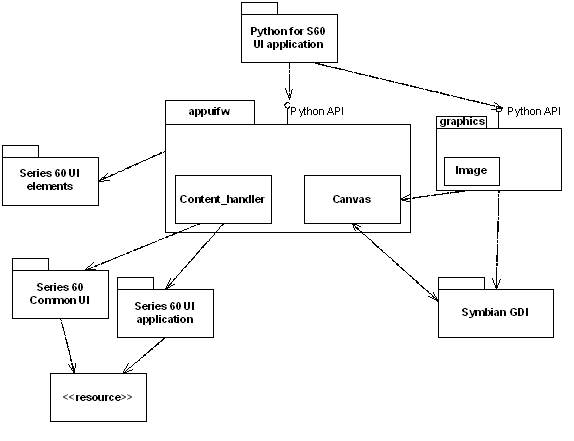
\includegraphics[width=\textwidth]{ui-overview}
\caption{Python for S60 UI environment overview}
\label{fig:ui-overview}
\end{figure}

\subsection{Basics of appuifw Module}
\label{subsec:basics}
Figure \ref{fig:normal-uilayout} shows the layout of a S60 application 
UI in the normal screen mode and a summary of how it relates to the services 
available at the \module{appuifw} API. For alternative layouts, see 
Figure \ref{fig:alternate-uilayouts}.

\begin{figure}
\centering
%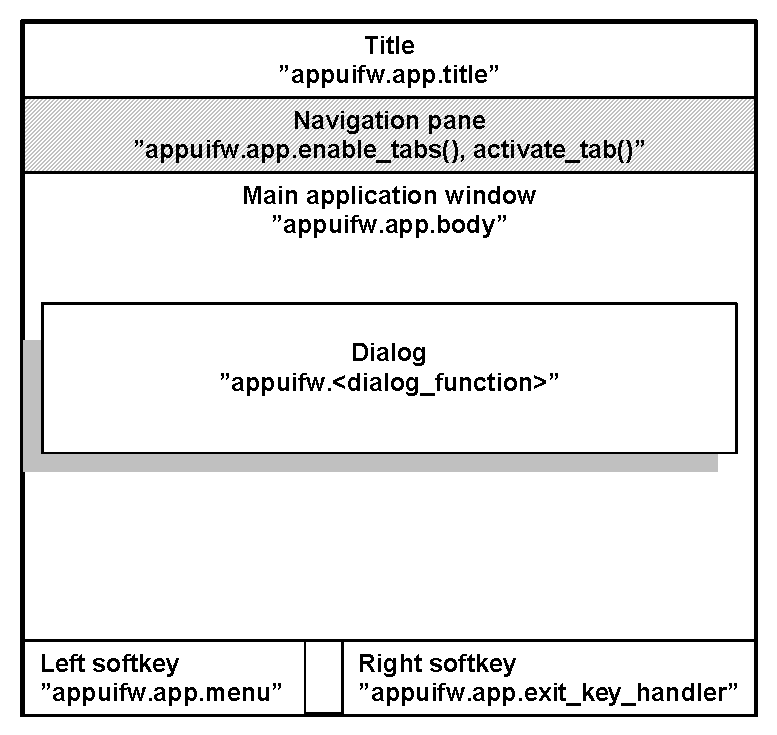
\includegraphics[width=0.7\textwidth]{screen-parts}
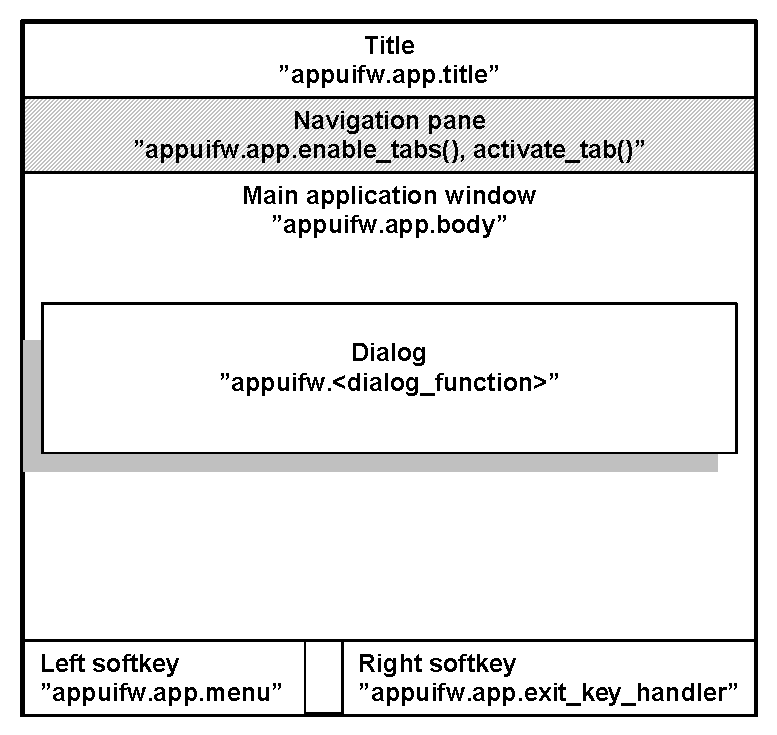
\includegraphics{screen-parts}
\caption{The different parts of the screen when using the 'normal' layout}
\label{fig:normal-uilayout}
\end{figure}

\begin{figure}
\centering
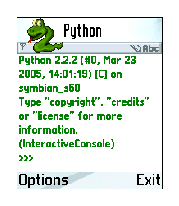
\includegraphics[width=\screenwidth]{layout-normal}
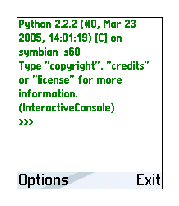
\includegraphics[width=\screenwidth]{layout-large}
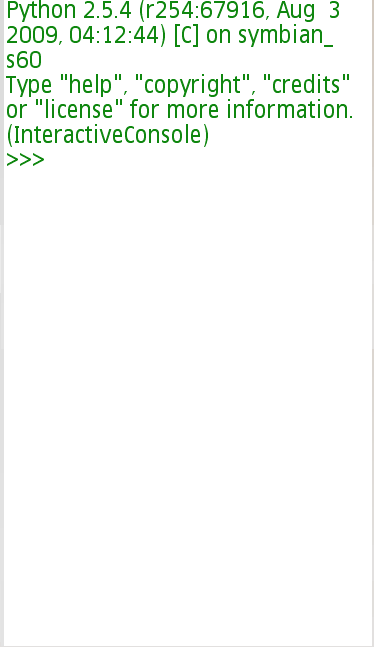
\includegraphics[width=\screenwidth]{layout-full}
\caption{UI layouts. left: 'normal', middle: 'large', right: 'full'}
\label{fig:alternate-uilayouts}
\end{figure}

The main application window may be set up to be occupied by a UI control.

A multi-view application can show the different views as tabs in the 
navigation pane and react as the users navigate between tabs. 

Dialogs always take precedence over the usual UI controls and appear on top 
of them.

UI controls are implemented as Python types. These types are available:

\begin{itemize}
\item \class{Text}
\item \class{Listbox}
\item \class{Canvas}
\end{itemize}
UI controls appear on the screen as soon as an instance of the corresponding 
Python type is set to the body field (\var{app.body}) of the current application UI.

\class{Form} is a versatile dialog implemented as a type.

The \class{Content_handler} type facilitates interfacing to other UI
applications and common high-level UI components. It is based on the
notion that designated handlers can reduce UI application interaction
to operations on MIME-type content.

The following dialogs are implemented as functions:

\begin{itemize}
\item \function{note}
\item \function{query}
\item \function{multi_query}
\item \function{selection_list}
\item \function{multi_selection_list}
\item \function{popup_menu}
\end{itemize}
A dialog becomes visible as soon as the corresponding Python function has 
been called. The function returns with the eventual user input or 
information on the cancellation of the dialog. \class{Form} is an 
exception; it is shown when its \method{execute} method is called.

\subsection{Softkeys}
\label{subsec:softkeys}
The softkeys are managed by the underlying S60 Platform. When no
dialog is visible, the right softkey is bound to application exit and
the left one represents an Options menu. Python for S60 offers
an interface for manipulating the menu and for binding the Exit key to
a Python-callable object (see Section \ref{subsec:application}). 

The native code that implements a dialog also manages the softkeys of the 
dialog, typically OK and Cancel. When the user input needs to be validated 
before accepting it and dismissing the dialog, it is best to use 
\class{Form}.

\subsection{Module Level Functions}
\label{subsec:module}
The following free functions - functions that do not belong to any class 
- are defined in the \module{appuifw} module:

\begin{funcdesc}{available_fonts}{}
Returns a list (Unicode) of all fonts available in the device.
\end{funcdesc}

\begin{funcdesc}{touch_enabled}{}
Returns 'True' if the device supports touch input, 'False' otherwise.
\end{funcdesc}

\begin{funcdesc}{query}{label, type\optional{, initial_value}}
Performs a query with a single-field dialog. The prompt is set to 
\var{label}, and the type of the dialog is defined by \var{type}. The 
value of \var{type} can be any of the following strings:

\begin{itemize}
\item \code{'text'}
\item \code{'code'}
\item \code{'number'}
\item \code{'date'}
\item \code{'time'}
\item \code{'query'}
\item \code{'float'}
\end{itemize}

The type of the optional \var{initial_value} parameter and the 
returned input depend on the value of \var{type}:

\begin{itemize}
\item For text fields, (\code{'text'}, \code{'code'}) it is Unicode
\item For number fields, it is numeric
\item For date fields, it is seconds since epoch rounded down to the nearest local midnight
\end{itemize}

A simple confirmation query and time query take no initial value and return 
\code{True/None} and seconds since local midnight, correspondingly. All 
queries return \code{None} if the users cancel the dialog. 

For \code{'float'} query the \var{initial_value} setting has no 
effect.
\end{funcdesc}


\begin{funcdesc}{multi_query}{label_1, label_2}
A two-field text (Unicode) input dialog. Returns the input values
as a 2-tuple. Returns \code{None} if the users cancel the dialog.
\end{funcdesc}

\begin{funcdesc}{note}{text\optional{, type\optional{, global}}}
Displays a note dialog of the chosen type with \var{text} 
(Unicode). The default value for \var{type} is \code{'info'}, which is 
automatically used if \var{type} is not set. \var{type} can be one of 
the following strings: \code{'error'}, \code{'info'} or 
\code{'conf'}. 

If \var{global} (integer) is any other value than zero a global note is 
displayed. A global note is displayed even if the Python application calling 
this function is in background. The same set of \var{type}s is supported as in 
standard note.
\end{funcdesc}

\begin{funcdesc}{popup_menu}{list\optional{, label}}
A pop-up menu style dialog. \var{list} representing the menu 
contents can be a list of Unicode strings or a list of Unicode string pairs 
(tuples). The resulting dialog list is then a single-style or a double-style 
list. A single-style list is shown in full; whereas a double-style list 
shows the items one at a time. Returns \code{None} if the user cancels the 
operation.
\end{funcdesc}

\begin{funcdesc}{selection_list}{choices\optional{, search_field=0}}
Executes a dialog that allows the users to select a list item and
returns the \var{index} of the chosen item, or \code{None} if the
selection is cancelled by the users. \var{choices} is a list of
Unicode strings.
\var{search_field} is \code{0} (disabled) by default and is optional. Setting it to \code{1} enables a search field (find pane) that facilitates searching for items in long lists. If enabled, the search field appears after you press a letter key.
\end{funcdesc}

\begin{funcdesc}{multi_selection_list}{choices\optional{, style='checkbox', search_field=0}}
  Executes a dialog that allows the users to select multiple list
  items.  Returns a tuple of indexes (a pair of Unicode strings) of
  the chosen items, or empty tuple if the no selection is made by
  the users. \var{choices} is a list of Unicode strings.  \var{style}
  is an optional string; the default value being \code{'checkbox'}.
  If \code{'checkbox'} is given, the list will be a checkbox list,
  where empty checkboxes indicate what items can be marked. The other
  possible value that can be set for \var{style} is
  \code{'checkmark'}. If \code{'checkmark'} is given, the list will be
  a markable list, which lists items but does not indicate
  specifically that items can be selected. To select items on a
  markable list, use the \var{'Options'} that has
  Mark/Unmark or the Edit key to select an item and the 
  Navigation key to browse the list. For example views on checkbox and
  markable lists, see
  \figurename~\ref{fig:checkbox-and-markable-list}.
  \var{search_field} is \code{0} (disabled) by default and is
  optional. Setting it to \code{1} enables a search field (find pane)
  that facilitates searching for items in long lists. If enabled, the
  search field is always visible with checkbox lists; with markable
  lists it appears by pressing a letter key.

Example:
\begin{verbatim}
tuple = appuifw.multi_selection_list([u'Harry', u'Ron', u'Hermione', u'Voldemort'], style='checkmark', search_field=1)
\end{verbatim}
\end{funcdesc}

\begin{figure}[htbp]
\centering
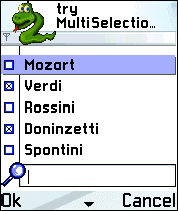
\includegraphics[width=\screenwidth]{checkbox-list}
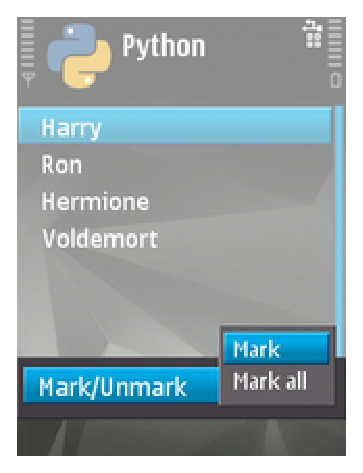
\includegraphics[width=\screenwidth]{markable-list}
\caption{Examples of a checkbox list (left) and a markable list (right)}
\label{fig:checkbox-and-markable-list}
\end{figure}

\subsection{Application Type}
\label{subsec:application}
A single implicit instance of this type always exists when \module{appuifw} 
module is present and can be referred to with the name \code{app}. New 
instances cannot be created by a Python program.

\begin{classdesc*}{Application}
Instances of \class{Application} type have the following attributes:

\begin{memberdesc}[Application]{body}
The UI control that is visible in the application's main window. Currently 
either \class{Text}, a \class{Listbox} object, \class{Canvas}, or 
\code{None}.
\end{memberdesc}

\begin{memberdesc}[Application]{directional_pad}
A boolean flag which controls the appearance of a virtual 4-way directional pad
that is displayed either at the bottom of the screen or on the right hand corner
depending on the orientation when using a Canvas. This is enabled by default on
devices that do not have a physical left and right soft key. This value is 
ignored on other devices, hence setting it to either True or False will have no effect.

Set it to \code{True} to enable 4-way directional pad and \code{False} to disable it.
\end{memberdesc}

\begin{memberdesc}[Application]{exit_key_handler}
A callable object that is called when the user presses the Exit softkey. 
Setting \member{exit_key_handler} to \code{None} sets it back to the 
default value.
\end{memberdesc}

\begin{memberdesc}[Application]{focus}
A callable object that is called with integer as parameter (0 = focus lost, 
1 = focus regained) when the application receives focus or it is switched to 
background. Focus is received e.g. when the application is switched from 
background to foreground or when the focus is regained from screensaver. 
Similarly when the screensaver is displayed, focus is lost.

Examples:
\begin{verbatim}
>>> import appuifw
>>> def cb(fg):
...   if(fg):
...     print "foreground"
...   else:
...     print "background"
...
>>> appuifw.app.focus=cb
>>> # switch to background, following text is printed from callback:
>>> background
>>> # switch to foreground, following text is printed from callback:
>>> foreground
\end{verbatim}

\begin{notice}
An improper callback can cause adverse effects. If you, for example,
define a callback which takes no parameters you will receive
never-ending \exception{TypeError} exceptions on the Nokia 6600.
\end{notice}

\end{memberdesc}

\begin{memberdesc}[Application]{menu}
This is a list of the following kinds of items:
\begin{itemize}
\item \code{(title, callback)} which creates a regular menu item
\item \code{(title, ((title, callback)\optional{...}))} which creates a submenu
\end{itemize}

\var{title} (Unicode) is the name of the item and \var{callback} the associated callable object. 
The maximum allowed number of items in a menu, or items in a submenu,
or submenus in a menu is 30.

Example:
\begin{verbatim}
appuifw.app.menu = [(u"Item 1", item1),
                    (u"Submenu 1", 
                        ((u"Subitem 1", subitem1),
                         (u"Subitem 2", subitem2)))]
\end{verbatim}
\end{memberdesc}

\begin{memberdesc}[Application]{orientation}
The orientation of the application. The orientation of the application can be 
one of the following values: \code{'automatic'} (this is the default value), 
\code{'portrait'} or \code{'landscape'}.
\end{memberdesc}

\begin{memberdesc}[Application]{screen}
The screen area used by an application. See \figurename~\ref{fig:alternate-uilayouts} for
example screens. The appearance of the application on the screen can
be affected by setting one of the following values: \code{'normal'},
\code{'large'} and \code{'full'}.

Examples:
\begin{verbatim}
appuifw.app.screen='normal'    # normal screen with title pane and softkey labels
appuifw.app.screen='large'     # only softkey labels visible
appuifw.app.screen='full'      # full screen mode on all devices
\end{verbatim}
\end{memberdesc}

\begin{memberdesc}[Application]{title}
The title of the application that is visible in the application's title
pane. Must be Unicode.
\end{memberdesc}

\begin{memberdesc}[Application]{track_allocations}
Set this to true if the interpreter should track all memory allocations and then
free the memory which was not explicitly released before application exit. The default
value of this attribute is true. As a consequence if there are any memory leaks in the
3rd party extension modules they will be released at the end. To check if there are
memory leaks(for debugging purposes) the following approach can be used :
\begin{verbatim}

appuifw.app.track_allocations = false

import my_extension
my_extension.do_something()

appuifw.app.track_allocations = true

\end{verbatim}
If the extension leaks memory then it will be reported at application exit.

\end{memberdesc}


Instances of \class{Application} type have the following methods:

\begin{methoddesc}[Application]{activate_tab}{index}
Activates the tab \var{index} counting from zero.
\end{methoddesc}

\begin{methoddesc}[Application]{full_name}{}
Returns the full name, in Unicode, of the native application in whose 
context the current Python interpreter session runs.
\end{methoddesc}

\begin{methoddesc}[Application]{layout}{layout_id}

Returns as a tuple the size and the position of the requested \code{layout_id}. 
The logical layouts are outlined partly in Figure \ref{fig:normal-uilayout}. The 
position is given from the top left corner. The \code{layout_id} can be one of 
the constants defined in module \module{appuifw}\footnote{Descriptions of the 
values are from the S60 SDK documentation \cite{S60Doc}.}:

\begin{datadesc}{EScreen} 
Screen.  
\end{datadesc}

\begin{datadesc}{EApplicationWindow} 
 Window that fills the entire screen.
\end{datadesc}

\begin{datadesc}{EStatusPane} 
Indicates common components for most of the applications.  
\end{datadesc}

\begin{datadesc}{EMainPane} 
The application main pane is used in all the applications.  
\end{datadesc}

\begin{datadesc}{EControlPane} 
Control pane.
\end{datadesc}

\begin{datadesc}{ESignalPane} 
The signal pane is used to indicate signal strength.  
\end{datadesc}

\begin{datadesc}{EContextPane} 
The context pane is used to indicate an active application.
\end{datadesc}

\begin{datadesc}{ETitlePane} 
Used to indicate the subject or the name of the main pane content. 
\end{datadesc}

\begin{datadesc}{EBatteryPane} 
The battery pane is used to indicate battery strength.  
\end{datadesc}

\begin{datadesc}{EUniversalIndicatorPane} 
The universal indicator pane is used to indicate items that require the user's 
attention while browsing applications. 
\end{datadesc}

\begin{datadesc}{ENaviPane} 
The navi pane is used to indicate navigation within an application, to provide 
context sensitive information to the user while entering or editing data, or to 
show additional information.  
\end{datadesc}

\begin{datadesc}{EFindPane} 
A fixed find pane is used with lists instead of the find pop-up window.  
\end{datadesc}

\begin{datadesc}{EWallpaperPane} 
Wallpaper pane.  
\end{datadesc}

\begin{datadesc}{EIndicatorPane} 
The universal indicator pane is used to indicate items that require the user's 
attention while browsing applications.  
\end{datadesc}

\begin{datadesc}{EAColumn} 
Used generally to display small sized graphics or heading texts.  
\end{datadesc}

\begin{datadesc}{EBColumn} 
Used generally to display large sized icons or heading texts.  
\end{datadesc}

\begin{datadesc}{ECColumn} 
Used generally to display data entered by the user. Overlaps with the D column. 
\end{datadesc}

\begin{datadesc}{EDColumn} 
Used generally to display additional icons. Overlaps with the C column. 
\end{datadesc}

\begin{datadesc}{EStaconTop} 
Top part of status and control panes in landscape layout.  
\end{datadesc}

\begin{datadesc}{EStaconBottom} 
Bottom part of status and control panes in landscape layout.  
\end{datadesc}

\begin{datadesc}{EStatusPaneBottom} 
Bottom part of status pane in landscape layout.  
\end{datadesc}

\begin{datadesc}{EControlPaneBottom} 
Bottom part of control pane in landscape layout.  
\end{datadesc}

\begin{datadesc}{EControlPaneTop} 
Top part of control pane in landscape layout.  
\end{datadesc}

\begin{datadesc}{EStatusPaneTop} 
Top part of status pane in landscape layout.
\end{datadesc}

Example:
\begin{verbatim}
>>> import appuifw
>>> appuifw.app.layout(appuifw.EMainPane)
((176, 144), (0, 44))
>>> # size and position (x, y) of the main pane in Nokia N70
\end{verbatim}

\end{methoddesc}

\begin{methoddesc}[Application]{set_exit}{}
Requests a graceful exit from the application as soon as the current script 
execution returns.
\end{methoddesc}

\begin{methoddesc}[Application]{set_tabs}{tab_texts\optional{,callback=None}}
Sets tabs with given names on them in the navigation bar; 
\var{tab_texts} is a list of Unicode strings. When the users 
navigate between tabs, \var{callback} gets called with the index 
of the active tab as an argument. Tabs can be disabled by giving an empty or 
one-item \var{tab_texts} list.
\end{methoddesc}

\begin{methoddesc}[Application]{uid}{}
Returns the UID, in Unicode, of the native application in whose 
context the current Python interpreter session runs.
\end{methoddesc}

\end{classdesc*}

\subsection{Form Type}
\label{subsec:form}
\class{Form} implements a dynamically configurable, editable multi-field 
dialog. \class{Form} caters for advanced dialog use cases with requirements 
such as free selectability of the combination of fields, possibility of 
validating the user input, and automatically producing the contents of some 
dialog fields before allowing the closing of the dialog. 

\begin{classdesc}{Form}{fields\optional{, flags=0}}
Creates a \class{Form} instance.
\var{fields} is a list of \emph{field descriptors}: \code{(label, type\optional{, value})} where

\var{label} is a Unicode string

\var{type} is one of the following strings: 
\code{'text'}, \code{'number'}, \code{'date'}, \code{'time'}, \code{'combo'}
or \code{'float'}

\var{value}, depending on \var{type}: Unicode string, numeric, float (seconds 
since Unix epoch rounded down to the nearest local midnight), float (seconds 
since local midnight), \code{([choice_label ...], index)} of float. For 
\code{'float'} \var{type} the initial value setting might not be shown in the 
UI.
\end{classdesc}

\class{Form} can also be configured and populated after construction. The 
configuration flags are visible as an attribute. \class{Form} implements 
the list protocol that can be used for setting the form fields, as well as 
obtaining their values after the dialog has been executed.

Instances of \class{Form} type have the following attributes:

\begin{memberdesc}[Form]{flags}
This attribute holds the values of the various configuration flags. 
Currently supported flags are:

\begin{datadesc}{FFormEditModeOnly}
When this flag is set, the form remains in edit mode while \method{execute} 
runs.
\end{datadesc}

\begin{datadesc}{FFormViewModeOnly}
When this flag is set, the form cannot be edited at all.
\end{datadesc}

\begin{datadesc}{FFormAutoLabelEdit}
This flag enables support for allowing the end-users to edit the labels of 
the form fields.
\end{datadesc}

\begin{datadesc}{FFormAutoFormEdit}
This flag enables automatic support for allowing the end-users to add and 
delete the form fields. Note that this is an experimental feature and is not 
guaranteed to work with all SDK versions.
\end{datadesc}

\begin{datadesc}{FFormDoubleSpaced}
When this flag is set, double-spaced layout is applied when the form is 
executed: one field takes two lines, as the label and the value field are on 
different lines.
\end{datadesc}
\end{memberdesc}

\begin{memberdesc}[Form]{menu}
A list of \code{(title, callback)} pairs, where 
each pair describes an item in the form's menu bar that is active while the 
dialog is being executed. \var{title} (Unicode) is the name of 
the item and \var{callback} the associated callable object.
\end{memberdesc}

\begin{memberdesc}[Form]{save_hook}
This attribute can be set to a callable object that receives one argument 
and returns a Boolean value. It gets called every time the users want to 
save the contents of an executing \class{Form} dialog. A candidate list for 
new form content - a list representing the currently visible state of the 
UI - is given as an argument. The list can be modified by 
\member{save_hook}. If \member{save_hook} returns \code{True}, the 
candidate list is set as the new contents of the form. Otherwise, the form 
UI is reset to reflect the field list contained in \class{Form} object.
\end{memberdesc}

Instances of \class{Form} type have the following methods:

\begin{methoddesc}[Form]{execute}{}
Executes the dialog by making it visible on the UI.
\end{methoddesc}

\begin{methoddesc}[Form]{insert}{index, field_descriptor}
Inserts the field descriptor into the \class{Form} before the given \var{index}.
\end{methoddesc}

\begin{methoddesc}[Form]{pop}{}
Removes the last field descriptor from the \class{Form} and returns it.
\end{methoddesc}

\begin{methoddesc}[Form]{length}{}the number of field descriptors in the form.
\end{methoddesc}

The subscript notation \code{f[i]} can be used to access or modify the
i-th element of the form \code{f}. Same limitations as discussed above
in the context of the flag \constant{FFormAutoFormEdit} apply to
modifying a form while it is executing. The ability to change the
schema of a form while it is executing is an experimental feature.

\subsection{Text Type}
\label{subsec:mylabel5}
\class{Text} is a text editor UI control. For examples on the options 
available with \class{Text}, see Figure \ref{fig:text-styles}.

\begin{figure}[htbp]
\centering
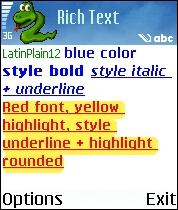
\includegraphics[width=\screenwidth]{text-styles-1}
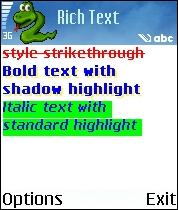
\includegraphics[width=\screenwidth]{text-styles-2}
\caption{Examples of the options available for Text type}
\label{fig:text-styles}
\end{figure}

Instances of \class{Text} type have the following attributes:

\begin{memberdesc}[Text]{color}
The color of the text. \code{color} supports the same color representation 
models as the \module{graphics} module. For the supported color 
representation models, see Section \ref{sec:graphics}.
\end{memberdesc}

\begin{memberdesc}[Text]{focus}
A Boolean attribute that indicates the focus state of the control. Editor 
control also takes the ownership of the navigation bar, and this feature is 
needed to enable the usage of this control in applications that use the 
navigation bar - for example, navigation tabs.
\end{memberdesc}

\begin{memberdesc}[Text]{font} 
The font of the text. There are two possible ways to set this attribute:

\begin{itemize}

\item Using a supported Unicode font, for example \code{u"Latin12"}. Trying to set a font which is not supported by the device has no effect. A list of supported fonts can be retrieved by using \function{appuifw.available_fonts}.

Example, setting font:
\begin{verbatim}
t = appuifw.Text()
t.font = u"albi17b" # sets font to Albi 17 bold
t.font = u"LatinPlain12" # sets font to Latin Plain 12
\end{verbatim}
\item Using one of the default device fonts that are associated with the following labels (plain strings):
\code{'annotation', 'title', 'legend', 'symbol', 'dense', 'normal'.}

Example, setting font: 
\begin{verbatim}
t.font = "title" # sets font to the one used in titles
\end{verbatim}

Example, checking the currently set font: 
\begin{verbatim}
unicodeFont = t.font
\end{verbatim}
\end{itemize}

The attribute value retrieved is always a Unicode string. If the font has 
been set with a label, for example, \code{'title'}, the attribute will 
retrieve the font associated with that label. 
\end{memberdesc}

\begin{memberdesc}[Text]{highlight_color}
The highlight color of the text. \code{highlight_color} supports the 
same color representation models as the \module{graphics} module. For the 
supported color representation models, see Section \ref{sec:graphics}.
\end{memberdesc}

\begin{memberdesc}[Text]{style}
The style of the text. The flags for this attribute are defined in the 
\module{appuifw} module. These flags can be combined by using the binary 
operator \code{|}. The flags can be divided into two types: text style 
and text highlight. Text style flags can be freely combined with each other. 
However, one or more text style flags can be combined with only one text 
highlight flag. The flags are:

Text style:

\begin{datadesc}{STYLE_BOLD} 
Enables bold text.
\end{datadesc}

\begin{datadesc}{STYLE_UNDERLINE}
Enables underlined text.
\end{datadesc}

\begin{datadesc}{STYLE_ITALIC} 
Enables italic text.
\end{datadesc}

\begin{datadesc}{STYLE_STRIKETHROUGH } 
Enables strikethrough.
\end{datadesc}

Text highlight:

\begin{datadesc}{HIGHLIGHT_STANDARD}
Enables standard highlight.
\end{datadesc}

\begin{datadesc}{HIGHLIGHT_ROUNDED}
Enables rounded highlight.
\end{datadesc}

\begin{datadesc}{HIGHLIGHT_SHADOW}
Enables shadow highlight.
\end{datadesc}

Only one highlight is allowed to be used at once. Therefore, it is possible 
to combine only one highlight with one or more text styles.

Examples:
\begin{verbatim}
t = appuifw.Text()

# These and other similar values and combinations are valid:
t.style = appuifw.STYLE_BOLD
t.style = appuifw.STYLE_UNDERLINE
t.style = appuifw.STYLE_ITALIC
t.style = appuifw.STYLE_STRIKETHROUGH
t.style = (appuifw.STYLE_BOLD|
	   appuifw.STYLE_ITALIC|
	   appuifw.STYLE_UNDERLINE)

# These values are valid:
t.style = appuifw.HIGHLIGHT_STANDARD
t.style = appuifw.HIGHLIGHT_ROUNDED
t.style = appuifw.HIGHLIGHT_SHADOW

# This combination is NOT valid:
# Invalid code, do not try!
t.style = (appuifw.HIGHLIGHT_SHADOW|appuifw.HIGHLIGHT_ROUNDED)
\end{verbatim}
\end{memberdesc}

Instances of \class{Text} type have the following methods:

\begin{methoddesc}[Text]{add}{text}
Inserts the Unicode string \var{text} to the current cursor position.
\end{methoddesc}

\begin{methoddesc}[Text]{bind}{event_code, callback}
Binds the callable Python object \var{callback} to event
\var{event_code}. The key codes are defined in 
the \module{key_codes} library module. The call 
\code{bind(event_code, None)} clears an 
existing binding. In the current implementation the event is always
passed also to the underlying native UI control.
\end{methoddesc}

\begin{methoddesc}[Text]{clear}{}
Clears the editor.
\end{methoddesc}

\begin{methoddesc}[Text]{delete}{\optional{pos=0, length=len()}}
Deletes \var{length} characters of the text held by the editor control, 
starting from the position \var{pos}.
\end{methoddesc}

\begin{methoddesc}[Text]{get_pos}{}
Returns the current cursor position.
\end{methoddesc}

\begin{methoddesc}[Text]{len}{}
Returns the length of the text string held by the editor control.
\end{methoddesc}

\begin{methoddesc}[Text]{get}{\optional{pos=0, length=len()}}
Retrieves \code{length} characters of the text held by the editor control, 
starting from the position \var{pos}.
\end{methoddesc}

\begin{methoddesc}[Text]{set}{text}
Sets the text content of the editor control to Unicode string 
\var{text}.
\end{methoddesc}

\begin{methoddesc}[Text]{set_pos}{cursor_pos}
Sets the cursor to \var{cursor_pos}.
\end{methoddesc}

\subsection{Listbox Type}
\label{subsec:listbox}

\begin{figure}[htbp]
\centering
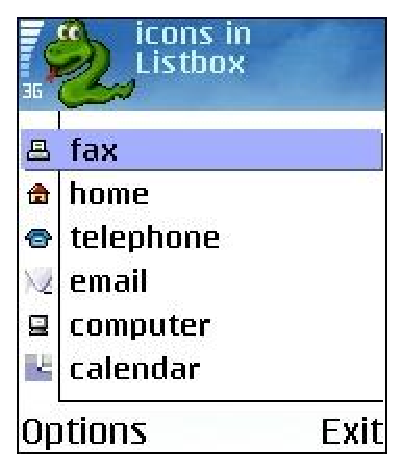
\includegraphics[width=\screenwidth]{listbox-with-icons}
\caption{Listbox with icons}
\label{fig:listbox-with-icons}
\end{figure}

An instance of this UI control type is visible as a listbox, also known as a 
list in Symbian, that can be configured to be a single-line item or a 
double-item listbox. Figure \ref{fig:listbox-with-icons} shows a single-line 
item Listbox with icons. For more information on the MBM and MIF formats, 
see Section \ref{subsec:icon}.

\begin{classdesc}{Listbox}{list, callback}
Creates a \class{Listbox} instance. A callable object 
\var{callback} gets called when a listbox selection has been 
made. \code{list} defines the content of the listbox and can be one of the 
following:

\begin{itemize}
\item A normal (single-line item) listbox: a list of Unicode strings, for example \code{[unicode_string item1, unicode_string item2]}
\item A double-item listbox: a two-element tuple of Unicode strings , for example \code{[(unicode_string item1, unicode_string item1description), (unicode_string item2, unicode_string item2description)]}
\item A normal (single-line item) listbox with graphics: a two-element tuple consisting of a Unicode string and an \class{Icon} object, for example \code{[(unicode_string item1, icon1), (unicode_string item2, icon2)]}.
\item A double-item listbox with graphics: a three-element tuple consisting of two Unicode strings and one \class{Icon} object, for example \code{[(unicode_string item1, unicode_string item1description, icon1), (unicode_string item2, unicode_string item2description, icon2)]}
\end{itemize}

Example: To produce a normal (single-line item) listbox with graphics:
\begin{verbatim}
icon1 = appuifw.Icon(u"z:\\resource\\apps\\avkon2.mbm", 28, 29)
icon2 = appuifw.Icon(u"z:\\resource\\apps\\avkon2.mbm", 40, 41)
entries = [(u"Signal", icon1),
           (u"Battery", icon2)]
lb = appuifw.Listbox(entries, lbox_observe)
\end{verbatim}
\end{classdesc}

\begin{notice}[note]
Known issue: Using this widget in large/full screen mode results in an unrefreshed area at the bottom of the screen.
\end{notice}

Instances of \class{Listbox} type have the following methods and properties:

\begin{methoddesc}[Listbox]{bind}{event_code, callback}
Binds the callable Python object \var{callback} to event 
\var{event_code}. The key codes are defined in 
the \module{key_codes} library module. The call
\code{bind(event_code, None)} clears an 
existing binding. In the current implementation the event is always passed 
also to the underlying native UI control.
\end{methoddesc}

\begin{methoddesc}[Listbox]{current}{}
Returns the currently selected item's index in the \class{Listbox}.
\end{methoddesc}

\begin{methoddesc}[Listbox]{set_list}{list\optional{, current}}
Sets the \class{Listbox} content to a list of Unicode strings or a
list of tuples of Unicode strings. The accepted structures of \var{list} are the
same as in the \class{Listbox} constructor. The optional argument \var{current} is the index of the focused list item.
\end{methoddesc}

\begin{memberdesc}[Listbox]{size}
The size of the \class{Listbox} as a tuple (width, height) - Read only.
\end{memberdesc}

\begin{memberdesc}[Listbox]{position}
The coordinates (as a tuple) of the top left corner of the \class{Listbox} -
Read only.
\end{memberdesc}

\subsection{Icon Type}
\label{subsec:icon}
An instance of \class{Icon} type encapsulates an icon to be used together 
with a \class{Listbox} instance. Note that currently \class{Icon} can only 
be used with \class{Listbox} (see Section \ref{subsec:listbox}).

MBM is the native Symbian OS format used for pictures. It is a
compressed file format where the files can contain several bitmaps and
can be referred to by a number. An \code{.mbg} file is the header file
usually associated with an \code{.mbm} file, which includes symbolic
definitions for each bitmap in the file. For example, an
\file{avkon.mbm} file has an associated index file called
\file{avkon.mbg}, which is included in S60 SDKs. For more information
on the MBM format and the bitmap converter tool, see \cite{S60Doc} and
search the topics with the key term "How to provide Icons"; this topic
also points you to the Bitmap Converter tool that can be used for
converting bitmaps into the MBM format.

\begin{classdesc}{Icon}{filename, bitmap, bitmapMask}
Creates an icon. \var{filename} is a Unicode file name and must 
include the whole path. Note that MBM is the only file formats supported.
\var{bitmap} and \var{bitmapMask} are integers that represent the index of 
the icon and icon mask inside that file respectively.
\end{classdesc}

Example: The following builds an icon with the standard signal symbol:
\begin{verbatim}
icon = appuifw.Icon(u"z:\\resource\\apps\\avkon2.mbm", 28, 29)
\end{verbatim}

\subsection{Content\_handler Type}
\label{subsec:content}

An instance of \class{Content_handler} handles data content by its MIME 
type.

\begin{classdesc}{Content_handler}{\optional{callback}}
Creates a \class{Content_handler} instance. A Content_handler handles
data content by its MIME type. The optional
\var{callback} is called when the embedded handler application 
started with the \method{open} method finishes. 
\end{classdesc}

Instances of \class{Content_handler} type have the following methods:

\begin{methoddesc}[Content_handler]{open}{filename}
Opens the file \var{filename} (Unicode) in its handler 
application if one has been registered for the particular MIME type. The 
handler application is embedded in the caller's thread. The call to this 
function returns immediately. When the handler application finishes, the 
\var{callback} that was given to the \class{Content_handler} 
constructor is called.
\end{methoddesc}

\begin{methoddesc}[Content_handler]{open_standalone}{filename}
Opens the file \var{filename} (Unicode) in its handler 
application if one has been registered for the particular MIME type. The 
handler application is started in its own process. The call to this function 
returns immediately. Note that \var{callback} is not called for 
applications started with this method.
\end{methoddesc}

\subsection{Canvas Type}
\label{subsec:canvas}
\class{Canvas} is a UI control that provides a drawable area on the screen 
and support for handling raw key events. \class{Canvas} supports the 
standard drawing methods that are documented in Section \ref{sec:graphics}.

\begin{classdesc}{Canvas}{\optional{redraw_callback=None, event_callback=None,
                                  resize_callback=None}}
Constructs a \class{Canvas}. The optional parameters are callbacks
that are called when specific events occur. 

\note{Watch out for cyclic
references here. For example, if the callbacks are methods of an
object that holds a reference to the \class{Canvas}, a reference cycle
is formed that must be broken at cleanup time or the
\class{Canvas} will not be freed.}

\var{redraw_callback} is called whenever a part of the \class{Canvas} 
has been obscured by something, is then revealed, and needs to be
redrawn. This can typically happen, for example, when the user
switches away from the Python application and back again, or after
displaying a pop-up menu. The callback takes as its argument a
four-element tuple that contains the top-left and the bottom-right
corner of the area that needs to be redrawn. In many cases redrawing
the whole
\class{Canvas} is a reasonable option. 

\var{event_callback} is called whenever a raw key event is received or when a 
pointer event occurs(only on touch input supported devices).
There are three kinds of key events: \code{EEventKeyDown},
\code{EEventKey}, and \code{EEventKeyUp}. When a user presses a key 
down, events \code{EEventKeyDown} and \code{EEventKey} are generated. 
When the key is released, an \code{EEventKeyUp} event is generated.

Pointer events are generated by touch input supported devices. When the screen
is touched the \code{EButton1Down} event is generated, \code{EDrag} while the
finger/stylus is dragged across the screen and then \code{EButton1Up} when the
finger/stylus is lifted.

The argument to the \var{event_callback} is a dictionary that contains 
the following data:

For key events:
\begin{itemize}
\item \code{'type'}: one of \code{EEventKeyDown}, \code{EEventKey}, or 
\code{EEventKeyUp}
\item \code{'keycode'}: the keycode of the key
\item \code{'scancode'}: the scancode of the key
\item \code{'modifiers'}: the modifiers that apply to this key event
\end{itemize}

For pointer events:
\begin{itemize}
\item \code{'type'}: one of the several pointer events - \code{EButton1Up}, 
\code{EButton1Down}, \code{EDrag} etc..
\item \code{'modifiers'}: the modifiers that apply to this pointer event
\item \code{'pos'}: A tuple containing the x-y pointer co-ordinates
\end{itemize}

Each key on the keyboard has one or more scancodes and zero or more keycodes 
associated with it. A scancode represents the physical key itself and a 
keycode is the result of state-related operating system defined processing 
done on the key. For keys that correspond to a symbol in the current 
character set of the phone, the keycode is equal to the code of the 
corresponding symbol in that character set. For example, if you are using 
the Nokia Wireless Keyboard (SU-8W), pressing the key A will always produce 
the scancode 65 (ASCII code for an upper case A), but the keycode 
could be either 65 or 91 (ASCII code for a lower case A) depending on 
whether or not the Shift key is pressed or Caps Lock is active. 

The \module{key_codes} module contains definitions for the keycodes and 
scancodes. See \figurename~\ref{fig:keyboard} for the codes of the most 
common keys on the phone keypad. 

Some keys are handled in a special way:

\begin{itemize}
\item A short press of the Edit key causes it to stay down, meaning that no \code{EEventKeyUp} event is sent. The event is only sent after a long press.
\item Detecting presses of the Voice tags key or the Power key is not supported.
\item If the right softkey is pressed, the \code{appuifw.app.exit_key_handler} callback is always executed.
\end{itemize}

There is no way to prevent the standard action of the Hang-up key, the Menu 
key, the Power key or the Voice tags key from taking place.

\begin{figure}
\centering
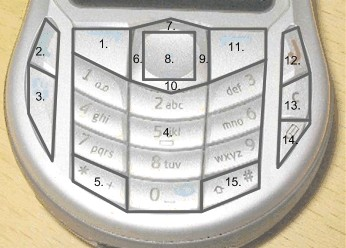
\includegraphics[width=5in]{6630keyboard}
%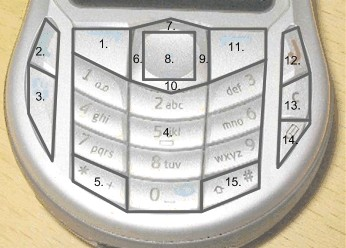
\includegraphics[width=3.60in,height=2.58in]{6630keyboard}
%\centerline{\includegraphics[width=3.60in,height=2.58in]{API_Reference_for_Python11.eps}} \par & 
\begin{tableiii}{lll}{textrm}{Key}{Keycode}{Scancode}
\lineiii{1.}{EKeyLeftSoftkey}{EScancodeLeftSoftkey}
\lineiii{2.}{EKeyYes}{EScancodeYes}
\lineiii{3.}{EKeyMenu}{EScancodeMenu}
\lineiii{4.}{EKey0...9}{EScancode0...9}
\lineiii{5.}{EKeyStar}{EScancodeStar}
\lineiii{6.}{EKeyLeftArrow}{EScancodeLeftArrow}
\lineiii{7.}{EKeyUpArrow}{EScancodeUpArrow}
\lineiii{8.}{EKeySelect}{EScancodeSelect}
\lineiii{9.}{EKeyRightArrow}{EScancodeRightArrow}
\lineiii{10.}{EKeyDownArrow}{EScancodeDownArrow}
\lineiii{11.}{EKeyRightSoftkey}{EScancodeRightSoftkey}
\lineiii{12.}{EKeyNo}{EScancodeNo}
\lineiii{13.}{EKeyBackspace}{EScancodeBackspace}
\lineiii{14.}{EKeyEdit}{EScancodeEdit}
\lineiii{15.}{EKeyHash}{EScancodeHash}
\end{tableiii}
\caption{Keycodes and scancodes for phone keys usable from Python applications}
\label{fig:keyboard}
\end{figure}

\var{resize_callback} is called when screen size is changed when the 
\class{Canvas} rect size has been changed. The callback takes as its argument a
two-element tuple that contains the new clientRect width and height. 

\end{classdesc}

Instances of \class{Canvas} type have the following methods:

\begin{methoddesc}[Canvas]{bind}{pointer_event, callable\optional{, ((x1, y1), (x2, y2))}}
This method can be used to listen to specific pointer events. The
\var{pointer_event} argument can be any one of the pointer events listed in the
\module{key_codes} module.

The most common pointer events are:

\begin{itemize}
\item \code{EButton1Down} - Pen down event 
\item \code{EButton1Up}   - Pen up event
\item \code{EDrag}        - Drag event (This event is only received when button1 is down)
\item \code{ESwitchOn}    - Switch on event caused by a screen tap.
\end{itemize}

\var{callable} is called when the pointer_event and the co-ordinate 
(if specified) criterion matches.

\var{((x1, y1), (x2, y2))} is an optional argument that can be passed to
specify the screen area to monitor for any specific pointer event. The two
co-ordinate tuple corresponds to the top-left and bottom-right points. This
argument will be ignored if the event is not a pointer event.

There are several ways in which bind can be used:

\begin{itemize}
\item \code{my_canv.bind(EButton1Up, callback)} - The callback is called when
EButton1Up event is generated anywhere in the canvas.

\item \code{my_canv.bind(EButton1Up, green_callback, ((x1, y1), (x2, y2)))} - The 
callback is called when the EButton1Up pointer event occurs inside the screen
area specified.

\item \code{my_canv.bind(EButton1Up, yellow_callback, ((x3, y3), (x4, y4)))} - 
Registers another callback for a different region but for the same pointer
event. When two screen areas overlap, the callback registered last will be
called when pointer events occur in the intersected region. 

\item \code{my_canv.bind(EButton1Up, callback3, ((x1, y1), (x2, y2)))} - If the
pointer event and the screen area to be monitored are the same, the callback
passed will replace the old callback already registered. 

\item \code{my_canv.bind(EButton1Up, None, ((x1, y1), (x2, y2)))} - If the pointer
event and the screen area to be monitored are the same, and the callback passed
is None, the callback registered previously is cleared.

\item \code{my_canv.bind(EButton1Up, None)} - All callbacks previously registered
for this pointer event are cleared, regardless of whether it was for a specific
screen area or for the entire canvas.
\end{itemize}

\begin{figure}
\centering
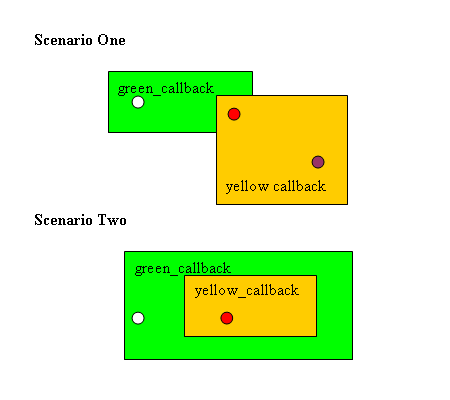
\includegraphics[width=5in]{bind-scenarios}
\caption{Canvas bind scenarios}
\label{fig:bind-scenarios}
\end{figure}

Clicking on the white spot should result in \code{green_callback} to be called. 
Clicking on the red spot should result in \code{yellow_callback} to be called in both
the scenarios shown above provided the \code{yellow_callback} was registered last. 
Clicking on the purple spot should result in \code{yellow_callback} to be called.

\end{methoddesc}

\begin{methoddesc}[Canvas]{begin_redraw}{\optional{((x1, y1), (x2, y2))}}
This is an explicit function that can be used to signal the window server that 
"I'm about to redraw this area". This method tells the window server that the 
window is about to respond to the last redraw event by redrawing the specified 
rectangle. This causes the window server to clear the rectangle, and remove it 
from the invalid region.
The optional co-ordinates x1, y1, x2, y2 should be the rectangle that has to be marked
for redrawing.

After the redraw is complete the application should call end_redraw().

\note{The begin_redraw and end_redraw methods should not be called inside the
redraw callback function.}

Couple of FAQs on redraw/non-redraw drawing:

Question: What is non-redraw drawing?
\begin{itemize}
\item "Non-redraw drawing" is any canvas/graphics drawing operation performed 
outside of begin_redraw()/end_redraw().
\end{itemize}

Question: What should applications do instead of non-redraw drawing?
\begin{itemize}
\item "Redraw drawing" is any drawing delimited by begin_redraw()/end_redraw().
\end{itemize}

Question: Why is non-redraw drawing bad for performance?
\begin{itemize}
\item The window server caches drawing operations in the redraw store.
Delimiting drawing with begin_redraw()/end_redraw() allows window server to 
efficiently manage drawing operations. 

If applications perform drawing operations outside begin_redraw/end_redraw,
window server cannot cull drawing operations from its cache of drawing 
operations, because it cannot know whether a set of drawing operations has 
been superceded by a new set.
In this scenario every frame of drawing that is done on a non-redraw drawing window 
will become slower and slower as it draws all the drawing operations for the 
entire history of the window (well actually up until the last begin_redraw/end_redraw 
for the whole window).

If an application performs begin_redraw/end_redraw, it tells the window server 
that it can throw away any old drawing operations it had for the area of the 
window specified in the redraw, thus allowing for more optimal management of 
drawing operations.
\end{itemize}

Question: What are the changes required for redraw drawing?
\begin{itemize}
\item Applications should delimit their drawing with begin_redraw()/end_redraw() 
- i.e. they should replace non-redraw drawing with redraw drawing. Sometimes, 
this is as straight forward as adding these calls to existing rendering code.
In other cases (where the application has been drawing using "incremental updates" 
to the window, the application drawing code would need to be reworked to perform a 
full refresh of the area redrawn for the rect provided in begin_redraw(rect).
\end{itemize}
\end{methoddesc}

\begin{methoddesc}[Canvas]{end_redraw}{}
Ends the current redraw. This function should be called when redrawing is complete.
\end{methoddesc}


Instances of \class{Canvas} type have the following attribute:

\begin{memberdesc}[Canvas]{size}
A two-element tuple that contains the current width and height of the 
\class{Canvas} as integers.
\end{memberdesc}

Instances of \class{Canvas} type have the same standard drawing methods 
that are documented in Section \ref{sec:graphics}.

\subsection{InfoPopup Type}
\label{subsec:infopopup}

An instance of \class{InfoPopup} type encapsulates an UI tip widget. This widget 
can be placed on top of other widgets to provide e.g. usage information to the 
user. The widget disappears as soon as the device's user presses any key or when 
the timer behind the \class{InfoPopup} is triggered.

\begin{classdesc}{InfoPopup}{}
Creates an \class{InfoPopup}.
\end{classdesc}

\begin{methoddesc}[InfoPopup]{show}{text, \optional{(x_coord, y_coord), 
time_shown, time_before, alignment}}
Show \var{text} (Unicode) in the \class{InfoPopup}. The optional parameters are 
the location (a tuple from the upper left corner), the time the popup is 
visible, \var{time_shown} (in milliseconds), the time before the popup, 
\var{time_before} (in milliseconds) and the alignment of the popup.

The default values are: the coordinates \code{(0, 0)}, \var{time_shown} 5 
seconds, \var{time_before} 0 seconds and for the alignment 
\code{appuifw.EHLeftVTop}.

The \var{alignment} can be one of the constants defined in module 
\code{appuifw}\footnote{Descriptions of the values are from the S60 SDK 
documentation \cite{S60Doc}.}:

\begin{datadesc}{EHLeftVTop} 
Object is left and top aligned. 
\end{datadesc}

\begin{datadesc}{EHLeftVCenter} 
Object is left aligned and centred vertically. 
\end{datadesc}

\begin{datadesc}{EHLeftVBottom} 
Object is left aligned and at the bottom. 
\end{datadesc}

\begin{datadesc}{EHCenterVTop} 
Object is centre aligned horizontally and at the top. 
\end{datadesc}

\begin{datadesc}{EHCenterVCenter} 
Object is centred horizontally and vertically. 
\end{datadesc}

\begin{datadesc}{EHCenterVBottom} 
Object is centred horizontally and at the bottom. 
\end{datadesc}

\begin{datadesc}{EHRightVTop} 
Object is right and top aligned. 
\end{datadesc}
 
\begin{datadesc}{EHRightVCenter} 
Object is right aligned and centred vertically. 
\end{datadesc}

\begin{datadesc}{EHRightVBottom} 
Object is right aligned and at the bottom. 
\end{datadesc}

\end{methoddesc}

\begin{methoddesc}[InfoPopup]{hide}{}
Hides the popup immediately.
\end{methoddesc}

Example:

\begin{verbatim}
>>> import appuifw
>>> i=appuifw.InfoPopup()
>>> i.show(u"Here is the tip.", (0, 0), 5000, 0, appuifw.EHRightVCenter)
>>>
\end{verbatim}

% Copyright (c) 2008-2009 Nokia Corporation
%
% Licensed under the Apache License, Version 2.0 (the "License");
% you may not use this file except in compliance with the License.
% You may obtain a copy of the License at
%
%     http://www.apache.org/licenses/LICENSE-2.0
%
% Unless required by applicable law or agreed to in writing, software
% distributed under the License is distributed on an "AS IS" BASIS,
% WITHOUT WARRANTIES OR CONDITIONS OF ANY KIND, either express or implied.
% See the License for the specific language governing permissions and
% limitations under the License.

\section{\module{globalui} --- 
    Interface to the S60 global UI notifiers }
\label{sec:globalui}

\declaremodule{extension}{globalui}
\platform{S60}
\modulesynopsis{Interface to the S60 global UI notifiers.}

The \module{globalui} module offers an interface to the S60 global UI notifiers. 
This allows a global note and query to be launched from an application which does not 
have a UI environment. 
The \module{globalui} module have functions:

\begin{funcdesc}{global_note}{note_text\optional{, type}}
Displays a note of the chosen type with \var{note_text} 
(Unicode). The default value for \var{type} is \code{'info'}. \var{type} can be 
one of the following strings: \code{'error'}, \code{'text'}, \code{'warn'}, \code{'charging'},
\code{'wait'}, \code{'perm'},\code{'not_charging'}, \code{'battery_full'}, \code{'battery_low'}, 
\code{'recharge_battery'}, or \code{'confirm'}. 
\end{funcdesc}

\begin{funcdesc}{global_query}{query_text\optional{, timeout}}
Displays a global confirmation query with \var{query_text} (Unicode). Returns 
\code{1} when the user presses 'Yes' and \code{0} otherwise. If the user does 
not respond to the query within \var{timeout} seconds, returns \code{None}. 
If the \var{timeout} value is 0, then the query waits indefinitely for user input. 
The default value for \var{timeout} is 0. The \var{timeout} value should be an integer.
\end{funcdesc}

\begin{funcdesc}{global_msg_query}{query_text, header_text\optional{, timeout}}
Displays a global message query with \var{query_text}(Unicode). \var{header_text} is used 
to set the heading string of the query. Returns \code{1} when the user 
presses 'OK' and \code{0} otherwise. If the user does not respond to the query within 
\var{timeout} seconds, returns \code{None}. If the \var{timeout} value is \code{0}, then the query 
waits indefinitely for user input. The default value for \var{timeout} is \code{0}. 
The \var{timeout} value should be an integer.
\end{funcdesc}

\begin{funcdesc}{global_popup_menu}{option_items\optional{, header_text, timeout}} 
Displays a global menu with \var{option_items}(Unicode). \var{header_text} is used to set the 
heading string of the menu. If no value is passed for \var{header_text}, then the header will
not be displayed. Returns the index value of the selected item from the list. If the user does
not respond to the menu within \var{timeout} seconds, returns \code{None}. If the \var{timeout}
value is \code{0}, then the menu waits indefinitely for the input. The default value for \var{timeout} 
is \code{0}. The \var{timeout} value should be an integer.
\end{funcdesc}

Example:
\begin{verbatim}
>>> import globalui, time
...
>>> text_to_show = u"text for showing note"
>>> globalui.global_note(text_to_show,'error')
>>> time.sleep(6)
>>> globalui.global_note(text_to_show)
>>> time.sleep(6)
>>> result = globalui.global_query(u"do you want to continue ?")
>>> time.sleep(6)
>>> listresult = globalui.global_popup_menu([u"MenuItem1", u"MenuItem2"],u"Select item",5)
...   
\end{verbatim}

% Copyright (c) 2005-2009 Nokia Corporation
%
% Licensed under the Apache License, Version 2.0 (the "License");
% you may not use this file except in compliance with the License.
% You may obtain a copy of the License at
%
%     http://www.apache.org/licenses/LICENSE-2.0
%
% Unless required by applicable law or agreed to in writing, software
% distributed under the License is distributed on an "AS IS" BASIS,
% WITHOUT WARRANTIES OR CONDITIONS OF ANY KIND, either express or implied.
% See the License for the specific language governing permissions and
% limitations under the License.

\section{\module{graphics} ---
  A graphics related services package}
\label{sec:graphics}

\declaremodule{extension}{graphics}
\platform{S60}
\modulesynopsis{A graphics related services package.}

The \module{graphics} module provides access to the graphics primitives and 
image loading, saving, resizing, and transformation capabilities provided by 
the Symbian OS. 

The module is usable from both graphical Python applications and
background Python processes. However, background processes have some
restrictions, namely that plain string symbolic font names are not
supported in background processes since background processes have no
access to the UI framework (see also Section
\ref{subsubsec:font-specs}).

For an example on using this module, see \cite{PyS60Prog}.

\subsection{Module Level Functions}
\label{subsec:mylabel7}
The following free functions - functions that do not belong to any class 
- are defined in the \module{graphics} module:

\begin{funcdesc}{screenshot}{}
Takes a screen shot and returns the image in \class{Image} format.
\end{funcdesc}

\subsection{Image Class Static Methods}
\label{subsec:image}
The following \class{Image} class static methods are defined in the 
\module{graphics} module:

\begin{funcdesc}{Image.new}{size\optional{, mode='RGB16'}}
Creates and returns a new \class{Image} object with the given size and 
mode. \var{size} is a two-element tuple. \var{mode} specifies the 
color mode of the \class{Image} to be created. It can be one of the 
following:

\begin{itemize}
\item \code{'1'}: Black and white (1 bit per pixel)
\item \code{'L'}: 256 gray shades (8 bits per pixel)
\item \code{'RGB12'}: 4096 colors (12 bits per pixel)
\item \code{'RGB16'}: 65536 colors (16 bits per pixel)
\item \code{'RGB'}: 16.7 million colors (24 bits per pixel)
\end{itemize}
It will also set the image size in twips according to the density of the device's primary screen. 
\end{funcdesc}

\begin{funcdesc}{Image.open}{filename}
Returns a new \class{Image} object (mode \code{RGB16}) that contains the 
contents of the named file. The supported file formats are JPEG and PNG. The 
file format is automatically detected based on file contents. 
\var{filename} should be a full path name.
\end{funcdesc}

\begin{funcdesc}{Image.inspect}{filename}
Examines the given file and returns a dictionary of the attributes of the 
file. At present the dictionary contains only the image size in pixels as a 
two-element tuple, indexed by key \code{'size'}. 
\var{filename} should be a full path name.
\end{funcdesc}

\subsection{Image Objects}
\label{subsec:image-objects}
An \class{Image} object encapsulates an in-memory bitmap. 

Note on asynchronous methods: Methods \method{resize}, \method{transpose}, 
\method{save}, and \method{load} have an optional callback argument. If the 
callback is not given, the method call is synchronous; when the method
returns, the operation is complete or an exception has been raised. If
the callback is given, the method calls are asynchronous. If all
parameters are valid and the operation can start, the method call will
return immediately.  The actual computation then proceeds in the
background. When it is finished, the callback is called with an error
code as the argument. If the given code is \code{0}, the operation
completed without errors, otherwise an error occurred.

It is legal to use an unfinished image as a source in a blit operation; this 
will use the image data as it is at the moment the blit is made and may thus 
show an incomplete result.

\class{Image} objects have the following methods:

\begin{methoddesc}[Image]{resize}{newsize\optional{, callback=None, keepaspect=0}}
Returns a new image that contains a resized copy of this image. If 
\var{keepaspect} is set to \code{1}, the resize will maintain the 
aspect ratio of the image, otherwise the new image will be exactly the given 
size. 

If \var{callback} is given, the operation is asynchronous, and the 
returned image will be only partially complete until \var{callback} is 
called.
\end{methoddesc}

\begin{methoddesc}[Image]{transpose}{direction\optional{, callback=None}}
Creates a new image that contains a transformed copy of this image. The 
\var{direction} parameter can be one of the following:

\begin{itemize}
\item \code{FLIP_LEFT_RIGHT}: Flips the image horizontally, exchanging left and right edges.
\item \code{FLIP_TOP_BOTTOM}: Flips the image vertically, exchanging top and bottom edges.
\item \code{ROTATE_90}: Rotates the image 90 degrees counterclockwise.
\item \code{ROTATE_180}: Rotates the image 180 degrees.
\item \code{ROTATE_270}: Rotates the image 270 degrees counterclockwise.
\end{itemize}

If \var{callback} is given, the operation is asynchronous and the 
returned image will be only partially complete until \var{callback} is 
called.
\end{methoddesc}

\begin{methoddesc}[Image]{load}{filename\optional{, callback=None}}
Replaces the contents of this \class{Image} with the contents of the named 
file, while keeping the current image mode. This \class{Image} object must 
be of the same size as the file to be loaded.

If \var{callback} is given, the operation is asynchronous and the loaded 
image will be only partially complete until \var{callback} is called. 
\var{filename} should be a full path name.
\end{methoddesc}

\begin{methoddesc}[Image]{save}{filename\optional{,callback=None, format=None, quality=75, bpp=24, compression='default'}}
Saves the image into the given file. The supported formats are JPEG and PNG. 
If \var{format} is not given or is set to \code{None}, the format is 
determined based on the file name extension: \code{'.jpg'} or 
\code{'.jpeg'} are interpreted to be in JPEG format and \code{'.png'} to 
be in PNG format. \var{filename} should be a full path name.

When saving in JPEG format, the \var{quality} argument specifies the 
quality to be used and can range from 1 to 100. 

When saving in PNG format, the \var{bpp} argument specifies how many bits 
per pixel the resulting file should have, and \var{compression} specifies 
the compression level to be used. 

Valid values for \var{bpp} are:

\begin{itemize}
\item \code{1}: Black and white, 1 bit per pixel
\item \code{8}: 256 gray shades, 8 bits per pixel
\item \code{24}: 16.7 million colors, 24 bits per pixel
\end{itemize}

Valid values for \var{compression} are:

\begin{itemize}
\item \code{'best'}: The highest possible compression ratio, the slowest speed
\item \code{'fast'}: The fastest possible saving, moderate compression
\item \code{'no'}: No compression, very large file size
\item \code{'default'}: Default compression, a compromise between file size and speed 
\end{itemize}

If \var{callback} is given, the operation is asynchronous. When the 
saving is complete, the \var{callback} is called with the result code.
\end{methoddesc}


\begin{methoddesc}[Image]{stop}{}
Stops the current asynchronous operation, if any. If an asynchronous call is 
not in progress, this method has no effect.
\end{methoddesc}

\class{Image} objects have the following attributes:

\begin{memberdesc}[Image]{size}
A two-element tuple that contains the size of the \class{Image}. Read-only.
\end{memberdesc}

\begin{memberdesc}[Image]{twipsize}
A two-element tuple that contains the size of the \class{Image} in twips. Read/Write.
\end{memberdesc}

\subsection{Common Features of Drawable Objects}
\label{subsec:common}
Objects that represent a surface that can be drawn on support a set of 
common drawing methods, described in this section. At present there are two 
such objects: \class{Canvas} from the \refmodule{appuifw} module and 
\class{Image} from the \module{graphics} module. 

\subsubsection{Options}
\label{subsubsec:options}
Many of these methods support a set of standard options. This set of options 
is as follows:

\begin{itemize}
\item \var{outline}: The color to be used for drawing outlines of primitives and text. If \code{None}, the outlines of primitives are not drawn.
\item \var{fill}: The color to be used for filling the insides of primitives. If \code{None}, the insides of primitives are not drawn. If \var{pattern} is also specified, \var{fill} specifies the color to be used for areas where the pattern is white.
\item \var{width}: The line width to be used for drawing the outlines of primitives.
\item \var{pattern}: Specifies the pattern to be used for filling the insides of primitives. If given, this must be either \code{None} or a 1-bit (black and white) \class{Image}.
\end{itemize}

\subsubsection{Coordinate representation}
\label{subsubsec:coordinate}
The methods accept an ordered set of coordinates in the form of a coordinate 
sequence. Coordinates can be of type \code{int}, \code{long}, or 
\code{float}. A valid coordinate sequence is a non-empty sequence of 
either

\begin{itemize}
\item Alternating x and y coordinates. In this case the sequence length must be even, or
\item Sequences of two elements, that specify x and y coordinates.
\end{itemize}
Examples of valid coordinate sequences:

\begin{itemize}
\item \code{(1, 221L, 3, 4, 5.85, -3)}: A sequence of three coordinates
\item \code{[(1,221L),(3,4),[5.12,6])}: A sequence of three coordinates
\item \code{(1,5)}: A sequence of one coordinate
\item \code{[(1,5)]}: A sequence of one coordinate
\item \code{[[1,5]]}: A sequence of one coordinate
\end{itemize}

Examples of invalid coordinate sequences:

\textbf{Invalid code, do not use!}
\begin{itemize}
\item \code{[]}: An empty sequence
\item \code{(1,2,3)}: Odd number of elements in a flat sequence
\item \code{[(1,2),(3,4),None]}: Contains an invalid element
\item \code{([1,2],3,4)}: Mixing the flat and nested form is not allowed
\end{itemize}

\subsubsection{Color representation}
\label{subsubsec:color}
All methods that take color arguments accept the following two color 
representations:

\begin{itemize}
\item A three-element tuple of integers in the range from 0 to 255 inclusive, representing the red, green, and blue components of the color.
\item An integer of the form \code{0xrrggbb}, where \code{rr} is the red, \code{gg} the green, and \code{bb} the blue component of the color. 
\end{itemize}
For 12 and 16 bit color modes the color component values are simply 
truncated to the lower bit depth. For the 8-bit grayscale mode images the 
color is converted into grayscale using the formula \code{(2*r+5*g+b)/8}, rounded 
down to the nearest integer. For 1-bit black and white mode images the color 
is converted into black (0) or white (1) using the formula \code{(2*r+5*g+b)/1024}.

Examples of valid colors:

\begin{itemize}
\item \code{0xffff00}: Bright yellow
\item \code{0x004000}: Dark green
\item \code{(255,0,0)}: Bright red
\item \code{0}: Black
\item \code{255}: Bright blue
\item \code{(128,128,128)}: Medium gray
\end{itemize}

Examples of invalid colors:

\textbf{Invalid code, do not use!}
\begin{itemize}
\item \code{(0,0.5,0.9)}: Floats are not supported
\item \code{'{\#}ff80c0'}: The HTML color format is not supported
\item \code{(-1,0,1000)}: Out-of-range values
\item \code{(1,2)}: The sequence is too short
\item \code{[128,128,192]}: This is not a tuple
\end{itemize}

\subsubsection{Font specifications}
\label{subsubsec:font-specs}
A font can be specified in three ways: 
\begin{itemize}
\item None, meaning the default font
\item a Unicode string that represents a full font name, such as \code{u'LatinBold19'}
\item a plain string symbolic name that refers to a font setting currently specified by 
the UI framework
\item as a two or three element tuple, where 
\begin{itemize}
\item the first element is the font name (unicode or string) or None for default font
\item the second element is the font height in pixels or None for default size
\item the third (optional) element is the flags applied to the font or None for default options.
\end{itemize}
\end{itemize}

The flags are the following:
\begin{itemize}
\item \code{FONT_BOLD} bold
\item \code{FONT_ITALIC} italic
\item \code{FONT_SUBSCRIPT} subscript
\item \code{FONT_SUPERSCRIPT} superscript
\item \code{FONT_ANTIALIAS} forces the font to be antialiased
\item \code{FONT_NO_ANTIALIAS} forces the font to not be antialiased
\end{itemize}

You can combine the flags with the binary or operator ``|''. For
example, the flags setting \code{FONT_BOLD|FONT_ITALIC} will produce
text that is both bold and italic.

Note: Antialiasing support is only available for scalable fonts.

You can obtain a list of all available fonts with the 
\module{appuifw} module function \function{available_fonts}.

The symbolic names for UI fonts are:
\begin{itemize}
\item \code{'normal'}
\item \code{'dense'}
\item \code{'title'}
\item \code{'symbol'}
\item \code{'legend'}
\item \code{'annotation'}
\end{itemize}
Since background processes have no access to the UI framework, these 
symbolic names are not supported in them. You need to specify the full font 
name.

\subsubsection{Common Methods of Drawable Objects}
\label{subsubsec:common}
\begin{methoddesc}{line}{coordseq\optional{, $<$options$>$}}
Draws a line connecting the points in the given coordinate sequence. For 
more information about the choices available for \var{options}, 
see Section \ref{subsubsec:options}.
\end{methoddesc}

\begin{methoddesc}{polygon}{coordseq\optional{, $<$options$>$}}
Draws a line connecting the points in the given coordinate sequence, and 
additionally draws an extra line connecting the first and the last point in 
the sequence. If a fill color or pattern is specified, the polygon is filled 
with that color or pattern. For more information about the choices available 
for \var{options}, see Section \ref{subsubsec:options}.
\end{methoddesc}

\begin{methoddesc}{rectangle}{coordseq\optional{, $<$options$>$}}
Draws rectangles between pairs of coordinates in the given sequence. The 
coordinates specify the top-left and the bottom- right corners of the 
rectangle. The sequence must have an even number of coordinates. For more 
information about the choices available for \var{options}, see 
Section \ref{subsubsec:options}.
\end{methoddesc}

\begin{methoddesc}{ellipse}{coordseq\optional{, $<$options$>$}}
Draws ellipses between pairs of coordinates in the given sequence. The
coordinates specify the top-left and bottom-right corners of the
rectangle inside which the ellipse is contained.  The sequence must
have an even number of coordinates. 
For more information about the choices available for \var{options}, see 
Section \ref{subsubsec:options}.
\end{methoddesc}

\begin{methoddesc}{pieslice}{coordseq, start, end\optional{, $<$options$>$}}
Draws pie slices contained in ellipses between pairs of coordinates in
the given sequence. The start and end parameters are floats that
specify the start and end points of pie slice as the starting and
ending angle in radians. The angle \code{0} is to the right, the angle
\code{pi/2} is straight up, \code{pi} is to the left and\code{-pi/2}
is straight down. \var{coordseq} is interpreted the same way as for
the \method{ellipse} method.
For more 
information about the choices available for \var{options}, see 
Section \ref{subsubsec:options}.
\end{methoddesc}

\begin{methoddesc}{arc}{coordseq, start, end\optional{, $<$options$>$}}
Draws arcs contained in ellipses between pairs of coordinates in
the given sequence. The start and end parameters are floats that
specify the start and end points of pie slice as the starting and
ending angle in radians. The angle \code{0} is to the right, the angle
\code{pi/2} is straight up, \code{pi} is to the left and\code{-pi/2}
is straight down. \var{coordseq} is interpreted the same way as for
the \method{ellipse} method.  For more information about the choices
available for \var{options}, see Section
\ref{subsubsec:options}.
\end{methoddesc}

\begin{methoddesc}{point}{coordseq\optional{, $<$options$>$}}
Draws points in each coordinate in the given coordinate sequence. If the 
\var{width} option is set to greater than 1, draws a crude approximation 
of a circle filled with the outline color in the locations. Note that
the approximation is not very accurate for large widths; use the
\method{ellipse} method if you need a precisely formed circle. 
For more information about the choices
available for \var{options}, see Section
\ref{subsubsec:options}.
\end{methoddesc}

\begin{methoddesc}{clear}{\optional{color=0xffffff}}
Sets the entire surface of the drawable to the given color, white by 
default.
\end{methoddesc}

\begin{methoddesc}{text}{coordseq, text\optional{fill=0, font=None}}
Draws the given text in the points in the given coordinate sequence
with the given color (default value is black) and the given font. The
font specification format is described above.
\end{methoddesc}

\begin{methoddesc}{measure_text}{text\optional{font=None, maxwidth=-1, maxadvance=-1}}
Measures the size of the given text when drawn using the given
font. Optionally you can specify the maximum width of the text or the
maximum amount the graphics cursor is allowed to move (both in pixels).

Returns a tuple of three values: 
\begin{itemize}
\item the bounding box for the text as a 4-tuple: (topleft-x, topleft-y, bottomright-x, bottomright-y)
\item the number of pixels the graphics cursor would move to the right
\item the number of characters of the text that fits into the given maximum width and advance
\end{itemize}
\end{methoddesc}

\begin{methoddesc}{blit}{image\optional{,target=(0,0), source=((0,0),image.size), mask=None, scale=0}}
Copies the source area from the given \var{image} to the target area
in this drawable. The source area is copied in its entirety if
\var{mask} is not given or is set to \code{None}. If the mask is
given, the source area is copied where the mask is white. \var{mask}
can be either \code{None}, a 1-bit (black and white) \class{Image} or
a grayscale \class{Image}, and must be of the same size as the source image. A grayscale mask acts
as an alpha channel, i.e. partial transparency.

\var{target} and \var{source} specify the target area in this image 
and the source area in the given source. They are coordinate sequences of 
one or two coordinates. If they specify one coordinate, it is interpreted as 
the upper-left corner for the area; if they specify two coordinates, they 
are interpreted as the top-left and bottom-right corners of the area.

If \var{scale} is other than zero, scaling is performed on the fly while 
copying the source area to the target area. If \var{scale} is zero, no 
scaling is performed, and the size of the copied area is clipped to the 
smaller of source and target areas.

Note that a \method{blit} operation with scaling is slower than one without 
scaling. If you need to blit the same \class{Image} many times in a scaled 
form, consider making a temporary \class{Image} of the scaling result and 
blitting it without scaling. Note also that the scaling performed by the 
\method{blit} operation is much faster but of worse quality than the one 
done by the \method{resize} method, since the \method{blit} method does not 
perform any antialiasing.
\end{methoddesc}

% Copyright (c) 2005-2009 Nokia Corporation
%
% Licensed under the Apache License, Version 2.0 (the "License");
% you may not use this file except in compliance with the License.
% You may obtain a copy of the License at
%
%     http://www.apache.org/licenses/LICENSE-2.0
%
% Unless required by applicable law or agreed to in writing, software
% distributed under the License is distributed on an "AS IS" BASIS,
% WITHOUT WARRANTIES OR CONDITIONS OF ANY KIND, either express or implied.
% See the License for the specific language governing permissions and
% limitations under the License.

\section{\module{camera} ---
    Interface for taking photographs and video recording}

\declaremodule{extension}{camera}
\label{sec:camera}
\platform{S60}

The \module{camera} module enables taking photographs and video recording.

The following data items for state information are available in \module{camera}:

\begin{datadesc}{EOpenComplete}
The opening of the video clip has succeeded.
\end{datadesc}

\begin{datadesc}{ERecordComplete}
The video recording has completed (not called on explicit \code{stop_recording} 
call).
\end{datadesc}

\begin{datadesc}{EPrepareComplete}
The device is ready to begin video recording.
\end{datadesc}

The \module{camera} module has the following functions\footnote{Descriptions 
for some of the values are based on information found in S60 SDK documentation 
\cite{S60Doc}}:

\begin{funcdesc}{cameras_available}{}
Returns the number of cameras available in the device.
\end{funcdesc}

\begin{funcdesc}{image_modes}{}
Returns the image modes supported in the device as a list of strings, for 
example: \code{['RGB12', 'RGB', 'JPEG_Exif', 'RGB16'].}
\end{funcdesc}

\begin{funcdesc}{image_sizes}{}
Returns the image sizes (resolution) supported in the device as a list of 
\code{(x, y)} tuples, for example: \code{[(640, 480), (160, 120)]}.
\end{funcdesc}

\begin{funcdesc}{flash_modes}{}
Returns the flash modes available in the device as a list of strings. 
\end{funcdesc}

\begin{funcdesc}{max_zoom}{}
Returns the maximum digital zoom value supported in the device as an 
integer. 
\end{funcdesc}

\begin{funcdesc}{exposure_modes}{}
Returns the exposure settings supported in the device as a list of strings. 
\end{funcdesc}

\begin{funcdesc}{white_balance_modes}{}
Returns the white balance modes available in the device as a list of 
strings. 
\end{funcdesc}

\begin{funcdesc}{take_photo}{\optional{mode, size, zoom, flash, exposure, white_balance, position}}
Takes a photograph and returns the image in:

\begin{enumerate}
  \item \code{Image} format (for more information on \code{Image} format, see 
  Chapter \ref{sec:graphics} \refmodule{graphics} Module) or
  
  \item Raw JPEG data\footnote{For more information, see e.g. 
  \url{http://en.wikipedia.org/wiki/JPEG}.}. 
\end{enumerate}

The settings listed below describe all settings that are supported by the 
\code{camera} module. You can retrieve the mode settings available for your 
device by using the appropriate functions listed at the beginning of this 
chapter.

\begin{itemize}

\item \var{mode} is the display mode of the image. The default value is 
\code{'RGB16'}. The following display modes are supported for the \code{Image} 
format pictures taken:
	\begin{itemize}
	\item \code{'RGB12'}: 4096 colors (12 bits per pixel)
	\item \code{'RGB16'}: 65536 colors (16 bits per pixel). Default value, always supported
	\item \code{'RGB'}: 16.7 million colors (24 bits per pixel)
	\end{itemize}

For the JPEG data format images the following modes are supported:

	\begin{itemize}
	\item \code{'JPEG_Exif'}: JPEG Exchangeable image file format
	\item \code{'JPEG_JFIF'}: JPEG File Interchange Format
	\end{itemize}

Note that there is variety between the devices and the supported formats.

\item \var{size} is the resolution of the image. The default value is \code{(640, 480)}. The following sizes are supported, for example, in Nokia 6630: \code{(1280, 960)}, \code{(640, 480)} and \code{(160, 120)}.
\item \var{flash} is the flash mode setting. The default value is \code{'none'}. The following flash mode settings are supported:
	\begin{itemize}
	\item \code{'none' \newline
}No flash. Default value, always supported
	\item \code{'auto' \newline
}Flash will automatically fire when required
	\item \code{'forced' \newline
}Flash will always fire
	\item \code{'fill_in' \newline
}Reduced flash for general lighting
	\item \code{'red_eye_reduce' \newline
}Red-eye reduction mode
	\end{itemize}
\item \var{zoom} is the digital zoom factor. It is assumed to be on a linear scale from 0 to the maximum zoom value allowed in the device. The default value is \code{0}, meaning that zoom is not used. 
\item \var{exposure} is the exposure adjustment of the device. Exposure is a combination of lens aperture and shutter speed used in taking a photograph. The default value is \code{'auto'.} The following exposure modes are supported:
	\begin{itemize}
	\item \code{'auto'} \newline
Sets exposure automatically. Default value, always supported
	\item \code{'night'} \newline
Night-time setting for long exposures
	\item \code{'backlight' } \newline
Backlight setting for bright backgrounds
	\item \code{'center'} \newline
Centered mode for ignoring surroundings
	\end{itemize}
\item \var{white_balance} can be used to adjust white balance to match the main source of light. The term white balance refers to the color temperature of the current light. A digital camera requires a reference point to represent white. It will then calculate all the other colors based on this white point. The default value for \var{white_balance} is \code{'auto'} and the following white balance modes are supported:
	\begin{itemize}
	\item \code{'auto'} \newline
Sets white balance automatically. Default value, always supported
	\item \code{'daylight'} \newline
Sets white balance to normal daylight
	\item \code{'cloudy}' \newline
Sets white balance to overcast daylight
	\item \code{'tungsten'} \newline
Sets white balance to tungsten filament lighting
	\item \code{'fluorescent}' \newline
Sets white balance to fluorescent tube lighting
	\item \code{'flash'} \newline
Sets white balance to flash lighting
	\end{itemize}
\item \var{position} is the camera used if the device, such as Nokia N95, has several cameras. In Nokia N95, the camera pointing to the user of the device is located in position \code{1}, whereas the one pointing away from the user is located in position \code{0}. The default \var{position} is \code{0}.
\end{itemize}

If some other application is using the camera, this operation fails, with error 
\code{SymbianError: KErrInUse}. Invoking this function right after the device 
boot, might result in \code{SymbianError: KErrNotReady} error.

In some Nokia devices (e.g. in N95), to be able to get the highest possible size 
for the captured image, you need to:

\begin{enumerate}
\item switch to the landscape mode (see \code{appuifw.app.orientation})
\item import the \code{camera} module
\item take the picture in the \code{'JPEG_Exif'} format.
\end{enumerate}

\item

\end{funcdesc}

\begin{funcdesc}{start_finder}{callable\optional{, backlight_on=1, size=main_pane_size}}

Starts the camera viewfinder and binds a callback to receive \code{Image} format 
feed. When a new viewfinder frame is ready the callback is invoked with the 
\code{Image} as parameter.

The optional parameter \code{backlight_on} determines whether the device 
backlight is kept on when the camera view finder is in operation. By default, 
the backlight is on (1 = on, 0 = off).

The optional parameter \code{size} (of type tuple, e.g. \code{(176, 144)}) can 
be used to change the size of the \code{Image} received in the callback. The 
default \code{size} is the same as the application's main pane size. 

Example view finder code:

\begin{verbatim}
>>> import appuifw
>>> import camera
>>> def cb(im):
...   appuifw.app.body.blit(im)
...
>>> import graphics
>>> appuifw.app.body=appuifw.Canvas()
>>> camera.start_finder(cb)
>>>
\end{verbatim}

\end{funcdesc}

\begin{funcdesc}{stop_finder}{}
Stops the viewfinder.
\end{funcdesc}

\begin{funcdesc}{release}{}
Releases the camera -- After invocation other applications can access the camera 
hardware.
\end{funcdesc}

\begin{funcdesc}{start_record}{filename, callable}
Starts video recording. \var{filename} is the file where the video clip is saved 
and \var{callable} will be called with possible error code (int) and status 
information (see data in module \module{camera}) as parameter.

Prior calling this function, the view finder needs to be started.
\end{funcdesc}

\begin{funcdesc}{stop_record}{}
Stops the video recording.
\end{funcdesc}

% Copyright (c) 2006 - 2009 Nokia Corporation
%
% Licensed under the Apache License, Version 2.0 (the "License");
% you may not use this file except in compliance with the License.
% You may obtain a copy of the License at
%
%     http://www.apache.org/licenses/LICENSE-2.0
%
% Unless required by applicable law or agreed to in writing, software
% distributed under the License is distributed on an "AS IS" BASIS,
% WITHOUT WARRANTIES OR CONDITIONS OF ANY KIND, either express or implied.
% See the License for the specific language governing permissions and
% limitations under the License.

\section{\module{keycapture} ---
         Interface for global capturing of key events.}
\label{sec:keycapture}

\declaremodule{extension}{keycapture}		% not standard, in C
\platform{S60}
\modulesynopsis{Interface for global capturing of key events.}

The \module{keycapture} module offers an API for global capturing of key events. The 
\module{keycapture} module provides the \class{KeyCapturer} object as a tool for listening to 
events.

The \class{KeyCapturer} object uses a callback method to report the key 
events. The callback method is called each time any of the specified keys 
is pressed.

Currently the \module{keycapture} module does not support capturing separate key-up or
key-down events.

\begin{notice}[note]
Keycapture module requires SwEvent capability.
\end{notice}

\subsection{Module Level Constants}
The following constants are defined in the \module{keycapture} module:

\begin{datadesc}{all_keys}
A list of all key codes defined in the \module{key_codes} module.
\end{datadesc}

\subsection{KeyCapturer objects} 
\label{KeyCapturer objects}

\class{KeyCapturer} object takes a callback method as a mandatory parameter to 
its constructor. The callback method must have one single parameter for 
forwarding the key code of the captured key.

There can be several \class{KeyCapturer} objects existing at the same time.

\class{KeyCapturer} object has following methods and properties:

\begin{memberdesc}[KeyCapturer]{keys}
List of keys to be captured. Can be read and written.
\\Example:
\begin{verbatim}
keys = (key_codes.EkeyUpArrow,)
keys = keycapture.all_keys
\end{verbatim} 
\end{memberdesc}

\begin{memberdesc}[KeyCapturer]{forwarding}
Specifies whether captured key events are forwarded to other applications or not.
Either has value 1 or 0. Can be read and written.
\end{memberdesc}

\begin{methoddesc}[KeyCapturer]{start}{}
Starts the actual capturing of key events.
\end{methoddesc}

\begin{methoddesc}[KeyCapturer]{stop}{}
Stops the actual capturing of key events.
\end{methoddesc}

\begin{methoddesc}[KeyCapturer]{last_key}{}
Returns last key code that is captured. 
\end{methoddesc}

% Copyright (c) 2006-2009 Nokia Corporation
%
% Licensed under the Apache License, Version 2.0 (the "License");
% you may not use this file except in compliance with the License.
% You may obtain a copy of the License at
%
%     http://www.apache.org/licenses/LICENSE-2.0
%
% Unless required by applicable law or agreed to in writing, software
% distributed under the License is distributed on an "AS IS" BASIS,
% WITHOUT WARRANTIES OR CONDITIONS OF ANY KIND, either express or implied.
% See the License for the specific language governing permissions and
% limitations under the License.

\section{\module{topwindow} ---
         Interface for creating windows that are shown on top of other 
         applications.}
\label{sec:topwindow}

\declaremodule{extension}{topwindow}
\platform{S60}
\modulesynopsis{Interface for creating windows that are shown on top of other 
         applications.}
         
The \module{topwindow} module offers an API for creating windows that are shown 
on top of other applications and managing the content of these windows. 
Images can be inserted into the windows and the background color, visibility, 
corner type and shadow of the window can be manipulated.

\module{topwindow} extension does not provide sophisticated drawing capabilities 
by any means but rather relies on services provided by the \module{graphics} 
extension: \module{topwindow} allows \module{graphics} \class{Image} objects to 
be put into the windows that are represented by \class{TopWindow} objects.

\class{TopWindow} object provides mainly only two services: \class{TopWindow} 
objects can be shown or hidden and Images can be put into the windows. However, 
several images can be added into one \class{TopWindow} object and several 
\class{TopWindow} objects can be created and shown. Since the images can be 
manipulated using the \module{graphics} extension this makes it possible to 
create many kind of content to the \class{TopWindow} objects.

\subsection{TopWindow objects}

\begin{classdesc}{TopWindow}{}
Create a \class{TopWindow} object.
\end{classdesc}

\class{TopWindow} objects have the following methods and properties:

\begin{methoddesc}[TopWindow]{show}{}
Shows the window. The window is not shown until show() is called.
\end{methoddesc}

\begin{methoddesc}[TopWindow]{hide}{}
Hides the window.
\end{methoddesc}

\begin{methoddesc}[TopWindow]{add_image}{image, position}
Inserts an image object \class{graphics.Image} into the window. The position 
of the image is specified by the \var(position) parameter. 
If only the coordinates of the top left corner are specified, like (x1, y1) 
the image is not resized. If four coordinates are given, like(x1, y1, x2, y2), 
the image is resized to fit to the specified area.
\\Example:
\begin{verbatim} 
add_image(image, (10,20))
add_image(image, (10,20,20,30))
\end{verbatim}
\end{methoddesc}

\begin{methoddesc}[TopWindow]{remove_image}{image\optional{,position}}
Removes the image from the window.
Mandatory parameter \var{image} must be a \class{graphics.Image} object. 
Parameter \var{position} may specify the top-left corner coordinates of the 
image or the rectangular area of the image. If only \var{image} parameter is 
given, all the pictures representing this image object are removed from the
window. If both parameters are given, only the picture that matches both 
parameters is removed.
\\Example:
\begin{verbatim}
remove_image(image)
remove_image(image, (10,10))
remove_image(image, (10,10,20,20))
\end{verbatim}
\end{methoddesc}

\begin{memberdesc}[TopWindow]{position}
Specifies the coordinates of the top left corner of the window. Can be read and written.
\\Example: 
\begin{verbatim}
position = (10, 20)
\end{verbatim}
\end{memberdesc}

\begin{memberdesc}[TopWindow]{size}
Specifies the size of the window. Can be read and written.
\\Example:
\begin{verbatim} 
size = (100, 200)
\end{verbatim}
\end{memberdesc}

\begin{memberdesc}[TopWindow]{images}
The images inserted into the window. Defined as a list of tuple objects. Each 
tuple contains a \class{graphics.Image} object and the \var{position} of the 
image. The \var{position} may specify the top-left coordinate of the image and 
optionally also the bottom-right coordinate of the image. Parameter (x,y) 
specifies the top-left coordinate, but does not resize the image while 
parameter like (x1,y1,x2,y2) specifies both the top-left and bottom-right 
coordinates and possibly also resizes the image. Can be read and written.
Also see the \method{add_image()} and \method{remove_image()} methods.
\\Example: 
\begin{verbatim}
images = [(image1,(x1,y1)), (image2,(x1,y1,x2,y2)), (image3,(50,50,100,100))]
\end{verbatim}
sets the window content to be 3 images. \code{image2} and \code{image3} are possibly resized 
while the \code{image1} is not)
\end{memberdesc}

\begin{memberdesc}[TopWindow]{shadow}
Specifies if the shadow of the window is shown and the length of the shadow. 
Can be read and written. Setting \code{shadow = 0} makes the shadow invisible.
\\Example: 
\code{shadow = 5}
\end{memberdesc}

\begin{memberdesc}[TopWindow]{corner_type}
Specifies the corner type of the window. Can be read and written. Corner type 
can be one of the following values: 
\begin{itemize}
\item \code{square}
\item \code{corner1}
\item \code{corner2}
\item \code{corner3}
\item \code{corner5}
\end{itemize}

Example: 
\code{corner_type = "square"}
\end{memberdesc}

\begin{memberdesc}[TopWindow]{maximum_size}
Returns the maximum size of the window as a tuple (width, height). Read only 
property.
\end{memberdesc}

\begin{memberdesc}[TopWindow]{background_color}
The background color of the window as an integer (e.g. \code{0xaabbcc}). The two 
greatest hexadecimal digits specify the red, the next two specify the blue and 
the last ones specify the green color. Can be read and written.
\\Example: 
\code{background_color = 0xffffff} (sets the white color)
\end{memberdesc}

\begin{memberdesc}[TopWindow]{visible}
Can be set to 0 or 1. 1 means that window is visible, 0 means that it is not. 
Can be read and written. Also see the \method{show} and \method{hide} methods.
\end{memberdesc}

% Copyright (c) 2005-2008 Nokia Corporation
%
% Licensed under the Apache License, Version 2.0 (the "License");
% you may not use this file except in compliance with the License.
% You may obtain a copy of the License at
%
%     http://www.apache.org/licenses/LICENSE-2.0
%
% Unless required by applicable law or agreed to in writing, software
% distributed under the License is distributed on an "AS IS" BASIS,
% WITHOUT WARRANTIES OR CONDITIONS OF ANY KIND, either express or implied.
% See the License for the specific language governing permissions and
% limitations under the License.

\section{\module{gles} ---
  Bindings to OpenGL ES}

\declaremodule{extension}{gles}
\platform{S60}
\modulesynopsis{Bindings to OpenGL ES.}
\label{sec:gles}

The \module{gles} module provides Python bindings to OpenGL ES 2D/3D graphics C
API. OpenGL ES is a standard defined by Khronos Group
(www.khronos.org). Currently S60 Python supports OpenGL ES version 1.0 from
Series 60 version 2.6 onwards. Support for OpenGL ES version 1.1 should also
become available in the near future, and both versions are documented
here. OpenGL ES 1.1 will require Series 60 version 3.0 or newer.

For detailed description of the OpenGL ES API see the official specifications at
http://www.khronos.org/opengles. This documentation contains only information
that is specific to the S60 Python bindings to OpenGL ES. Where possible, the
conventions of the PyOpenGL desktop OpenGL bindings
(http://pyopengl.sourceforge.net) have been followed.

The display of OpenGL ES graphics is handled by separate module,
\module{glcanvas}. See \module{glcanvas} module documentation for more
information.

\subsection{array type}

\module{gles} module defines \class{array} type for representing numerical data of
specific GL type. \class{array} objects are convenient when numerical data for
OpenGL ES calls is specified in Python code. Class \class{array} also defines
the standard Python sequence methods so its instances can be iterated and
individual items in arrays can be manipulated easily.

\begin{classdesc}{array}{type, dimension, sequence}
Constructs a new \class{array} object that contains the given type of data that
is taken from \var{sequence}. Parameter \var{dimension} specifies how many items
there are in each array element. The dimension information is stored with the
array and is used by those functions that need to know the element size of the
input data, for example, if colors are specified with three or four
components. The dimension does not affect the length of an array or its
indexing: both are based on individual items.

Value of \var{type} must be one of the following:
\code{GL_FLOAT}, \code{GL_BYTE}, \code{GL_UNSIGNED_BYTE}, \code{GL_SHORT},
\code{GL_UNSIGNED_SHORT}, or \code{GL_FIXED}.

The data in \var{sequence} is flattened before it is used to fill the
array. When \var{type} is \code{GL_FLOAT}, the sequence can contains floats or
integers. With all other types, \var{sequence} must only contain
integers. Values in \var{sequence} are casted in C to the requested type, so if
the requested type cannot properly represent all the values the results can be
unexpected.

\begin{methoddesc}[array]{__len__}{}
Returns the number of items in the array. Note that array dimension does not
affect the calculation of the length.
\end{methoddesc}

\begin{methoddesc}[array]{__getitem__}{index}
Returns the item in array with \var{index}. Note that array dimension does not
affect indexing.
\end{methoddesc}

\begin{methoddesc}[array]{__setitem__}{index, value}
Sets the value of the item in position \var{index} to \var{value}. Note that
array dimension does not affect indexing.
\end{methoddesc}
\end{classdesc}

\subsection{Error handling}

Errors generated by the API calls are handled similarly as in PyOpenGL: all GL
errors are reported as Python exceptions of type \class{gles.GLerror}. The
wrapper code checks GL error status after each call automatically. There is no
Python binding for \code{glGetError} call.

\subsection{Differences to OpenGL ES C API}
\label{subsec:differences}

Certain OpenGL ES functions require special handling in Python, mainly because
of the pointer parameters in the C API. Additionally, special Python versions for
some OpenGL ES functions have been added. Both of sets of functions are
documented below. If a function is not listed here its Python version should
exactly match the C version defined in the official OpenGL ES 1.0 and 1.1
specifications.

\subsubsection{OpenGL ES 1.0}

\begin{funcdesc}{glColorPointer}{size, type, stride, sequence}
Parameter \var{sequence} must be either a \class{gles.array} object or some other
Python sequence object. \class{gles.array} objects require less processing and can
be therefore slightly faster. If \class{gles.array} object is used, the type and
dimension of its data are ignored and \var{size} and \var{type} are used
instead.
\end{funcdesc}

\begin{funcdesc}{glColorPointerub}{sequence}
Special Python version of \code{glColorPointer} that accepts either a
\class{gles.array} object or some other Python sequence object. Other parameters
of \code{glColorPointer} will be determined as follows:
\begin{itemize}
\item \var{size} If \var{sequence} is an instance of \class{gles.array}, its dimension is used; otherwise the length of \var{sequence} is used.
\item \var{type} \code{GL_UNSIGNED_BYTE}
\item \var{stride} 0
\end{itemize}
\end{funcdesc}

\begin{funcdesc}{glColorPointerf}{sequence}
Special Python version of \code{glColorPointer} that behaves exactly as
\code{glColorPointerub} except \code{GL_FLOAT} is used as \var{type}.
\end{funcdesc}

\begin{funcdesc}{glColorPointerx}{sequence}
Special Python version of \code{glColorPointer} that behaves exactly as
\code{glColorPointerub} except \code{GL_FIXED} is used as \var{type}.
\end{funcdesc}

\begin{funcdesc}{glCompressedTexImage2D}{target, level, internalformat, width, height, border, imageSize, data}
Parameter \var{data} must be either a \class{gles.array} or a Python string.
\end{funcdesc}

\begin{funcdesc}{glCompressedTexSubImage2D}{target, level, xoffset, yoffset, width, height, format, imageSize, data}
Parameter \var{data} must be either a \class{gles.array} or a Python string.
\end{funcdesc}

\begin{funcdesc}{glDeleteTextures}{sequence}
Parameter \var{sequence} must be a Python sequence containing integers.
\end{funcdesc}

\begin{funcdesc}{glDrawElements}{mode, count, type, indices}
Parameter \var{indices} must be either a \class{gles.array} or some other Python
sequence object. \class{gles.array} objects require less processing and can be
therefore slightly faster. If \class{gles.array} object is used, the type of its
data is ignored and \var{type} is used instead.
\end{funcdesc}

\begin{funcdesc}{glDrawElementsub}{mode, indices}
Special Python version of \code{glDrawElements} that uses length of the sequence
\var{indices} as \var{count} and \code{GL_UNSIGNED_BYTE} as \var{type}.
\end{funcdesc}

\begin{funcdesc}{glDrawElementsus}{mode, indices}
Special Python version of \code{glDrawElements} that uses length of the sequence
\var{indices} as \var{count} and \code{GL_UNSIGNED_SHORT} as \var{type}.
\end{funcdesc}

\begin{funcdesc}{glFogv}{pname, params}
Parameter \var{params} must be a Python sequence containing float values.
\end{funcdesc}

\begin{funcdesc}{glFogxv}{pname, params}
Parameter \var{params} must be a Python sequence containing integer values.
\end{funcdesc}

\begin{funcdesc}{glGenTextures}{n}
The generated texture names are returned in a Python tuple.
\end{funcdesc}

\begin{funcdesc}{glGetIntegerv}{pname}
The values are returned in a Python tuple.
\end{funcdesc}

\begin{funcdesc}{glGetString}{name}
The value is return as a Python string.
\end{funcdesc}

\begin{funcdesc}{glLightModelfv}{pname, params}
Parameter \var{params} must be a Python sequence containing float values.
\end{funcdesc}

\begin{funcdesc}{glLightModelxv}{pname, params}
Parameter \var{params} must be a Python sequence containing integer values.
\end{funcdesc}

\begin{funcdesc}{glLightfv}{light, pname, params}
Parameter \var{params} must be a Python sequence containing float values.
\end{funcdesc}

\begin{funcdesc}{glLightxv}{light, pname, params}
Parameter \var{params} must be a Python sequence containing integer values.
\end{funcdesc}

\begin{funcdesc}{glLoadMatrixf}{m}
Parameter \var{m} must be a Python sequence containing float values. The sequence
is flattened before its items are read.
\end{funcdesc}

\begin{funcdesc}{glLoadMatrixx}{m}
Parameter \var{m} must be a Python sequence containing integer values. The
sequence is flattened before its items are read.
\end{funcdesc}

\begin{funcdesc}{glMaterialfv}{face, pname, params}
Parameter \var{params} must be a Python sequence containing float values.
\end{funcdesc}

\begin{funcdesc}{glMaterialxv}{face, pname, params}
Parameter \var{params} must be a Python sequence containing integer values.
\end{funcdesc}

\begin{funcdesc}{glMultMatrixf}{m}
Parameter \var{m} must be a Python sequence containing float values. The
sequence is flattened before its items are read.
\end{funcdesc}

\begin{funcdesc}{glMultMatrixx}{m}
Parameter \var{m} must be a Python sequence containing integer values. The
sequence is flattened before its items are read.
\end{funcdesc}

\begin{funcdesc}{glNormalPointer}{type, stride, sequence}
Parameter \var{sequence} must be either a \class{gles.array} object or some other
Python sequence object. \class{gles.array} objects require less processing and
can be therefore slightly faster. If \class{gles.array} object is used, the type
of its data is ignored and \var{type} is used instead.
\end{funcdesc}

\begin{funcdesc}{glNormalPointerb}{sequence}
Special Python version of \code{glNormalPointer} that uses \var{type}
\code{GL_BYTE} and \var{stride} 0.
\end{funcdesc}

\begin{funcdesc}{glNormalPointers}{sequence}
Special Python version of \code{glNormalPointer} that uses \var{type}
\code{GL_SHORT} and \var{stride} 0.
\end{funcdesc}

\begin{funcdesc}{glNormalPointerf}{sequence}
Special Python version of \code{glNormalPointer} that uses \var{type}
\code{GL_FLOAT} and \var{stride} 0.
\end{funcdesc}

\begin{funcdesc}{glNormalPointerx}{sequence}
Special Python version of \code{glNormalPointer} that uses \var{type}
\code{GL_FIXED} and \var{stride} 0.
\end{funcdesc}

\begin{funcdesc}{glReadPixels}{x, y, width, height, format, type}
The pixel data read is returned in a Python string.
\end{funcdesc}

\begin{funcdesc}{glTexCoordPointer}{size, type, stride, sequence}
Parameter \var{sequence} must be either a \class{gles.array} object or some other
Python sequence object. \class{gles.array} objects require less processing and
can be therefore slightly faster. If \class{gles.array} object is used, the
dimension and type of its data are ignored and \var{size} and \var{type} are
used instead.
\end{funcdesc}

\begin{funcdesc}{glTexCoordPointerb}{sequence}
Special Python version of \code{glTexCoordPointer} that accepts either a
\class{gles.array} object or some other Python sequence object. Other parameters
 of \code{glTexCoordPointer} will be determined as follows:
\begin{itemize}
\item \var{size} If \var{sequence} is an instance of \class{gles.array}, its dimension is used; otherwise the length of \var{sequence} is used.
\item \var{type} \code{GL_BYTE}
\item \var{stride} 0
\end{itemize}
\end{funcdesc}

\begin{funcdesc}{glTexCoordPointers}{sequence}
Special Python version of \code{glTexCoordPointer} that behaves exactly as
\code{glTexCoordPointerb} except \code{GL_SHORT} is used as \var{type}.
\end{funcdesc}

\begin{funcdesc}{glTexCoordPointerf}{sequence}
Special Python version of \code{glTexCoordPointer} that behaves exactly as
\code{glTexCoordPointerb} except \code{GL_FLOAT} is used as \var{type}.
\end{funcdesc}

\begin{funcdesc}{glTexCoordPointerx}{sequence}
Special Python version of \code{glTexCoordPointer} that behaves exactly as
\code{glTexCoordPointerb} except \code{GL_FIXED} is used as \var{type}.
\end{funcdesc}

\begin{funcdesc}{glTexEnvfv}{face, pname, params}
Parameter \var{params} must be a Python sequence containing float values.
\end{funcdesc}

\begin{funcdesc}{glTexEnvxv}{face, pname, params}
Parameter \var{params} must be a Python sequence containing integer values.
\end{funcdesc}

\begin{funcdesc}{glTexImage2D}{target, level, internalformat, width, height, border, format, type, pixels}
Parameter \var{pixels} must be either a Python string, a \class{gles.array}
object, or \class{graphics.Image} object. Python strings are taken as literal
data with no conversion. The dimension and type of data in \class{gles.array}
objects are ignored: the raw data in the array is used.

Use of \class{graphics.Image} objects is limited to only some combinations of
\var{format} and \var{type}. Table \ref{tab:image2d} below shows the accepted
combinations. To get the best results and performance, the \class{CFbsBitmap}
object in the \class{graphics.Image} object should be in the equivalent display
mode, also shown in the table below. Otherwise, the \class{CFbsBitmap} object
will be first converted to the equivalent display mode before reading its pixel
data, which can degrade the visual quality in some cases.
\begin{table}[htbp]
\begin{center}
\begin{tabular}{l|l|l}
\hline
\var{format} & \var{type} & The equivalent display mode \\
\hline
GL_LUMINANCE, GL_ALPHA & GL_UNSIGNED_BYTE & EGray256 \\
\hline
GL_RGB & GL_UNSIGNED_BYTE & EColor16M \\
\hline
GL_RGB & GL_UNSIGNED_SHORT_5_6_5 & EColor64K \\
\hline
\end{tabular}
\caption{Legal combinations of format and type with the equivalent Symbian display mode}
\label{tab:image2d}
\end{center}
\end{table}
\end{funcdesc}

\begin{funcdesc}{glTexSubImage2D}{target, level, xoffset, yoffset, width, height, format, type, pixels}
The handling of \var{pixels} is the same as with \code{glTexImage2D}.
\end{funcdesc}

\begin{funcdesc}{glVertexPointer}{size, type, stride, sequence}
Parameter \var{sequence} must be either a \class{gles.array} object or some other
Python sequence object. \class{gles.array} objects require less processing and
can be therefore slightly faster. If \class{gles.array} object is used, the
dimension and type of its data are ignored and \var{size} and \var{type} are
used instead.
\end{funcdesc}

\begin{funcdesc}{glVertexPointerb}{sequence}
Special Python version of \code{glVertexPointer} that accepts either a
\class{gles.array} object or some other Python sequence object.
Other parameters of \code{glVertexPointer} will be determined as follows:
\begin{itemize}
\item \var{size} If \var{sequence} is an instance of \class{gles.array}, its dimension is used; otherwise the length of \var{sequence} is used.
\item \var{type} \code{GL_BYTE}
\item \var{stride} 0
\end{itemize}
\end{funcdesc}

\begin{funcdesc}{glVertexPointers}{sequence}
Special Python version of \code{glVertexPointer} that behaves exactly as
\code{glVertexPointerb} except \code{GL_SHORT} is used as \var{type}.
\end{funcdesc}

\begin{funcdesc}{glVertexPointerf}{sequence}
Special Python version of \code{glVertexPointer} that behaves exactly as
\code{glVertexPointerb} except \code{GL_FLOAT} is used as \var{type}.
\end{funcdesc}

\begin{funcdesc}{glVertexPointerx}{sequence}
Special Python version of \code{glVertexPointer} that behaves exactly as
\code{glVertexPointerb} except \code{GL_FIXED} is used as \var{type}.
\end{funcdesc}

\subsubsection{OpenGL ES 1.1}

\begin{funcdesc}{glBufferData}{target, size, data, usage}
Parameter \var{data} must be a \class{gles.array} object. If \var{size} is -1,
the in-memory size of \var{data} is used in its place.
\end{funcdesc}

\begin{funcdesc}{glBufferDatab}{target, data, usage}
Special Python version of \code{glBufferData} that accepts either a
\class{gles.array} object or some other Python sequence object for \var{data}.
If \class{gles.array} object is used, its in-memory size in bytes is used as
\var{size}. Other sequences are first converted to flat lists of
\code{GL_BYTE} data by casting. The length of the resulting sequence in bytes
is used as \var{size}.
\end{funcdesc}

\begin{funcdesc}{glBufferDataub}{target, data, usage}
Special Python version of \code{glBufferData} that works exactly like
\code{glBufferDatab} except \code{GL_UNSIGNED_BYTE} is used instead of
\code{GL_BYTE}.
\end{funcdesc}

\begin{funcdesc}{glBufferDatas}{target, data, usage}
Special Python version of \code{glBufferData} that works exactly like
\code{glBufferDatab} except \code{GL_SHORT} is used instead of \code{GL_BYTE}.
\end{funcdesc}

\begin{funcdesc}{glBufferDataus}{target, data, usage}
Special Python version of \code{glBufferData} that works exactly like
\code{glBufferDatab} except \code{GL_UNSIGNED_SHORT} is used instead of
\code{GL_BYTE}.
\end{funcdesc}

\begin{funcdesc}{glBufferDataf}{target, data, usage}
Special Python version of \code{glBufferData} that works exactly like
\code{glBufferDatab} except \code{GL_FLOAT} is used instead of \code{GL_BYTE}.
\end{funcdesc}

\begin{funcdesc}{glBufferDatax}{target, data, usage}
Special Python version of \code{glBufferData} that works exactly like
\code{glBufferDatab} except \code{GL_FIXED} is used instead of \code{GL_BYTE}.
\end{funcdesc}

\begin{funcdesc}{glBufferSubData}{target, size, data, usage}
Parameter \var{data} must be a \class{gles.array} object. If \var{size} is -1,
the in-memory size of \var{data} is used in its place.
\end{funcdesc}

\begin{funcdesc}{glBufferSubDatab}{target, data, usage}
Special Python version of \code{glBufferSubData} that accepts either a
\class{gles.array} object or some other Python sequence object for \var{data}.
If \class{gles.array} object is used, its in-memory size (in bytes) is used as
\var{size}. Other sequences are first converted to flat lists of
\code{GL_BYTE} data by casting. The length of the resulting sequence is used as
\var{size}.
\end{funcdesc}

\begin{funcdesc}{glBufferSubDataub}{target, data, usage}
Special Python version of \code{glBufferSubData} that works exactly like
\code{glBufferSubDatab} except \code{GL_UNSIGNED_BYTE} is used instead of
\code{GL_BYTE}.
\end{funcdesc}

\begin{funcdesc}{glBufferSubDatas}{target, data, usage}
Special Python version of \code{glBufferSubData} that works exactly like
\code{glBufferSubDatab} except \code{GL_SHORT} is used instead of \code{GL_BYTE}.
\end{funcdesc}

\begin{funcdesc}{glBufferSubDataus}{target, data, usage}
Special Python version of \code{glBufferSubData} that works exactly like
\code{glBufferSubDatab} except \code{GL_UNSIGNED_SHORT} is used instead of
\code{GL_BYTE}.
\end{funcdesc}

\begin{funcdesc}{glBufferSubDataf}{target, data, usage}
Special Python version of \code{glBufferSubData} that works exactly like
\code{glBufferSubDatab} except \code{GL_FLOAT} is used instead of \code{GL_BYTE}.
\end{funcdesc}

\begin{funcdesc}{glBufferSubDatax}{target, data, usage}
Special Python version of \code{glBufferSubData} that works exactly like
\code{glBufferSubDatab} except \code{GL_FIXED} is used instead of
\code{GL_BYTE}.
\end{funcdesc}

\begin{funcdesc}{glClipPlanef}{plane, equation}
Parameter \var{equation} must be a Python sequence that contains four float
values.
\end{funcdesc}

\begin{funcdesc}{glClipPlanex}{plane, equation}
Parameter \var{equation} must be a Python sequence that contains four integer
values.
\end{funcdesc}

\begin{funcdesc}{glDeleteBuffers}{buffers}
Parameter \var{buffers} must be a Python sequence that contains integer values.
\end{funcdesc}

\begin{funcdesc}{glDrawTexsvOES}{coords}
Parameter \var{coords} must be a Python sequence that contains integer
values. 
\end{funcdesc}

\begin{funcdesc}{glDrawTexivOES}{coords}
Parameter \var{coords} must be a Python sequence that contains integer
values. 
\end{funcdesc}

\begin{funcdesc}{glDrawTexfvOES}{coords}
Parameter \var{coords} must be a Python sequence that contains float values.
\end{funcdesc}

\begin{funcdesc}{glDrawTexfvOES}{coords}
Parameter \var{coords} must be a Python sequence that contains integer values.
\end{funcdesc}

\begin{funcdesc}{glGenBuffers}{n}
The generated buffer names are returned in a Python tuple.
\end{funcdesc}

\begin{funcdesc}{glGetBooleanv}{pname}
The values are returned in a Python tuple.
\end{funcdesc}

\begin{funcdesc}{glGetBufferParameteriv}{target, pname}
The value is returned as an integer.
\end{funcdesc}

\begin{funcdesc}{glGetClipPlanef}{plane}
The values are returned in a Python tuple.
\end{funcdesc}

\begin{funcdesc}{glGetClipPlanef}{plane}
The values are returned in a Python tuple.
\end{funcdesc}

\begin{funcdesc}{glGetFixedv}{pname}
The values are returned in a Python tuple.
\end{funcdesc}

\begin{funcdesc}{glGetFloatv}{pname}
The values are returned in a Python tuple.
\end{funcdesc}

\begin{funcdesc}{glGetLightfv}{light, pname}
The values are returned in a Python tuple.
\end{funcdesc}

\begin{funcdesc}{glGetLightxv}{light, pname}
The values are returned in a Python tuple.
\end{funcdesc}

\begin{funcdesc}{glGetMaterialfv}{face, pname}
The values are returned in a Python tuple.
\end{funcdesc}

\begin{funcdesc}{glGetMaterialxv}{face, pname}
The values are returned in a Python tuple.
\end{funcdesc}

\begin{funcdesc}{glGetTexEnvf}{face, pname}
The values are returned in a Python tuple.
\end{funcdesc}

\begin{funcdesc}{glGetTexEnvx}{face, pname}
The values are returned in a Python tuple.
\end{funcdesc}

\begin{funcdesc}{glGetTexParameterf}{target, pname}
The value is returned as a float.
\end{funcdesc}

\begin{funcdesc}{glGetTexParameterx}{target, pname}
The value is returned as an integer.
\end{funcdesc}

\begin{funcdesc}{glMatrixIndexPointerOES}{size, type, stride, sequence}
Parameter \var{sequence} must be either a \class{gles.array} object or some other
Python sequence object. \class{gles.array} objects require less processing and
can be therefore slightly faster. If \class{gles.array} object is used, the
dimension and type of its data are ignored and \var{size} and \var{type} are
used instead.
\end{funcdesc}

\begin{funcdesc}{glMatrixIndexPointerOESub}{sequence}
Special Python version of \code{glMatrixIndexPointerOES} that accepts either a
\class{gles.array} object or some other Python sequence object.
Other parameters of \code{glMatrixIndexPointerOES} will be determined as follows:
\begin{itemize}
\item \var{size} If \var{sequence} is an instance of \class{gles.array}, its dimension is used; otherwise the length of \var{sequence} is used.
\item \var{type} \code{GL_UNSIGNED_BYTE}
\item \var{stride} 0
\end{itemize}
\end{funcdesc}

\begin{funcdesc}{glPointParameterfv}{pname, params}
Parameter \var{params} must be a Python sequence containing float values.
\end{funcdesc}

\begin{funcdesc}{glPointParameterxv}{pname, params}
Parameter \var{params} must be a Python sequence containing integer values.
\end{funcdesc}

\begin{funcdesc}{glPointSizePointerOES}{type, stride, sequence}
Parameter \var{sequence} must be either a \class{gles.array} object or some other
Python sequence object. \class{gles.array} objects require less processing and
can be therefore slightly faster. If \class{gles.array} object is used, the type
of its data is ignored and \var{type} is used instead.
\end{funcdesc}

\begin{funcdesc}{glPointSizePointerOESf}{sequence}
Special Python version of \code{glPointSizePointerOES} uses \code{GL_FLOAT} as
\var{type} and 0 as \var{stride}.
\end{funcdesc}

\begin{funcdesc}{glPointSizePointerOESx}{target, data, usage}
Special Python version of \code{glPointSizePointerOES} uses \code{GL_FIXED} as
\var{type} and 0 as \var{stride}.
\end{funcdesc}

\begin{funcdesc}{glWeightPointerOES}{size, type, stride, sequence}
Parameter \var{sequence} must be either a \class{gles.array} object or some other
Python sequence object. \class{gles.array} objects require less processing and
can be therefore slightly faster. If \class{gles.array} object is used, the
dimension and type of its data are ignored and \var{size} and \var{type} are
used instead.
\end{funcdesc}

\begin{funcdesc}{glWeightPointerOESf}{sequence}
Special Python version of \code{glWeightPointerOES} that accepts either a
\class{gles.array} object or some other Python sequence object.
Other parameters of \code{glWeightPointerOES} will be determined as follows:
\begin{itemize}
\item \var{size} If \var{sequence} is an instance of \class{gles.array}, its dimension is used; otherwise the length of \var{sequence} is used.
\item \var{type} \code{GL_FLOAT}
\item \var{stride} 0
\end{itemize}
\end{funcdesc}

\begin{funcdesc}{glWeightPointerOESx}{sequence}
Special Python version of \code{glWeightPointerOES} that behaves exactly as
\code{glWeightPointerOESf} except \code{GL_FIXED} is used as \var{type}.
\end{funcdesc}

% Copyright (c) 2005-2009 Nokia Corporation
%
% Licensed under the Apache License, Version 2.0 (the "License");
% you may not use this file except in compliance with the License.
% You may obtain a copy of the License at
%
%     http://www.apache.org/licenses/LICENSE-2.0
%
% Unless required by applicable law or agreed to in writing, software
% distributed under the License is distributed on an "AS IS" BASIS,
% WITHOUT WARRANTIES OR CONDITIONS OF ANY KIND, either express or implied.
% See the License for the specific language governing permissions and
% limitations under the License.

\section{\module{glcanvas} ---
  UI Control for Displaying OpenGL ES Graphics}
\label{sec:glcanvas}

\declaremodule{extension}{glcanvas}
\platform{S60}
\modulesynopsis{UI Control for Displaying OpenGL ES Graphics}

The \module{glcanvas} module provides a UI control, \class{GLCanvas}, for
displaying OpenGL ES graphics. \class{GLCanvas} component is similar to the
\module{appuifw} \class{Canvas} component that supports Symbian OS -level
drawing.

Internally \class{GLCanvas} uses EGL for displaying the OpenGL ES graphics. EGL,
as OpenGL ES, is a standard API defined by the Khronos Group
(www.khronos.org). Specifically, \class{GLCanvas} uses an EGL window surface,
which supports double-buffered rendering. It is possible to affect selection of
the EGL config that is used to create the window surface; for details, see the
documentation of the \class{GLCanvas} constructor.

\class{GLCanvas} instances also hold the OpenGL ES context object, which
together with the surface, are needed for rendering. When one wants to render
with a specific OpenGL ES context to a specific surface, they need to be
\emph{made current}. This also applies to \class{GLCanvas}, which has the
\code{makeCurrent} method for this purpose. Generally, calling
\code{makeCurrent} has to be done only if multiple \class{GLCanvas} objects are
used in the same program, as each \class{GLCanvas} object is automatically made
current when it is created and it remains current until it is destroyed or
\code{makeCurrent} of some other \class{GLCanvas} object is called.

\begin{classdesc}{GLCanvas}{redraw_callback, \optional{event_callback=None, resize_callback=None, attributes=None}}
Constructs a new \class{GLCanvas} object that can be used as a UI control for
displaying OpenGL ES graphics. Parameters \var{redraw_callback},
\var{event_callback}, and \var{resize_callback} have the same meaning as with
\module{appuifw} module \class{Canvas}. Using \var{redraw_callback} to specify
the OpenGL ES drawing is preferred as it will be automatically called by
\code{drawNow} method.

Parameter \var{attributes} can be used to specify attributes used in EGL config
selection. It must be a Python dictionary where keys are EGL attribute names
(which are defined in the \module{glcanvas} module) and values are integers
defining the desired attribute values. Unless specified in \var{attributes},
\code{EGL_BUFFER_SIZE} is set to value based on the display mode of the window
owned by the underlying \class{CCoeControl} object and \code{EGL_DEPTH_SIZE} is
set to 16. Attributes specified in \var{attributes} are given to
\code{eglChooseConfig}. Refer to the EGL specification for a detailed list of
config attributes and explanation of how the selection of EGL configs works.

The new \class{GLCanvas} object will be made current when the constructor
returns so \code{makeCurrent} does not have to be called before starting to use
OpenGL ES calls.

\begin{methoddesc}[GLCanvas]{bind}{key_code, c \optional{, ((x1, y1), (x2, y2))}}
Sets a callback to be called when a specific key is pressed or pointer event occurs. Parameter
\var{key_code} should be one of the standard Symbian key codes defined in
\module{key_codes}. Parameter \var{c} must be a callable object. The optional
two co-ordinate tuple corresponds to the top left and bottom right points of the
rectangle to be monitored for pointer events. This argument is ignored for Key events.

For different bind scenarios refer \class{Canvas}'s bind method.
\end{methoddesc}

\begin{methoddesc}[GLCanvas]{drawNow}{}
Calls the redraw callback (if set) and then calls \code{eglSwapBuffers} to
render and display the OpenGL ES graphics.
\end{methoddesc}

\begin{methoddesc}[GLCanvas]{makeCurrent}{}
Makes this \class{GLCanvas} object current, meaning that it will be used to
display the results of the subsequent OpenGL ES calls. In EGL terms this means
that the EGL context and surface held by this object will be passed to
\code{eglMakeCurrent}. Using \code{makeCurrent} makes it possible to use several
\class{GLCanvas} objects in a single application: the receiver of the OpenGL ES
calls can be switched with \code{makeCurrent} easily.
\end{methoddesc}
\end{classdesc}

% Copyright (c) 2005-2007 Nokia Corporation
%
% Licensed under the Apache License, Version 2.0 (the "License");
% you may not use this file except in compliance with the License.
% You may obtain a copy of the License at
%
%     http://www.apache.org/licenses/LICENSE-2.0
%
% Unless required by applicable law or agreed to in writing, software
% distributed under the License is distributed on an "AS IS" BASIS,
% WITHOUT WARRANTIES OR CONDITIONS OF ANY KIND, either express or implied.
% See the License for the specific language governing permissions and
% limitations under the License.

\section{\module{sensor} ---
  Module to access the device sensors.}
\label{sec:sensor}

\declaremodule{extension}{sensor}
\platform{S60}
\modulesynopsis{Module to access the device sensors.}

\subsection{Module for devices that support S60 Sensor API}
\label{subsec:sensorapi}

The \module{Sensor} module offers direct access to a device's physical sensors. It has been tested with the following sensors:
\begin{itemize}
\item acceleration sensor: raises events about the 3-axes acceleration of the device
\item tapping sensor: raises an event when the device was tapped twice on the front side
\item rotation sensor: raises an event based on the orientation of the device.
\end{itemize}

Instead of passing on raised events, event filtering is also supported. Two 
examples of using an event filter are also provided by the \module{Sensor} 
module, namely the class \class{OrientationEventFilter} and 
\class{RotEventFilter}. Both filters can be used to raise events when the 
orientation changes in the device (For example, when it is turned to the right). The support 
is device dependent. For example, Nokia 5500 supports \class{OrientationEventFilter} and 
Nokia N95 supports \class{RotEventFilter}.

\begin{notice}[note]
The module \module{Sensor} is available from S60 3rd Edition onwards. 
(inclusive).
\end{notice}

\subsubsection{Module Level Functions}

On the module level, \module{Sensor} provides the following functions:

\begin{funcdesc}{sensors}{}

Returns a dictionary containing all available sensors. The format of the dictionary is as follows:

\begin{verbatim}
{
  { 'sensor name 1': { 'id': sensor_id_1, 'category': category_id_1 } },
  { 'sensor name 2': { 'id': sensor_id_2, 'category': category_id_2 } },
  ...
}
\end{verbatim}

with \code{sensor_id_X} and \code{category_id_X} being integer values.

\end{funcdesc}

\subsubsection{Constants}

The following \code{orientation} constants are used by the \class{OrientationEventFilter} class.
Callbacks which have been connected to a \class{Sensor} object that utilises the
\class{OrientationEventFilter} event filter will receive one of these constants as an argument
upon a detected orientation change. The names of the constant are the side of the device that
is currently turned upwards from your point of view. (For example \code{FRONT} means that
the device is lying on its back - its front side is turned upwards.)

\begin{memberdesc}{orientation.TOP}
Represents the orientation where the device is held upwards.
\end{memberdesc}

\begin{memberdesc}{orientation.BOTTOM}
Represents the orientation where the device is held upside down.
\end{memberdesc}

\begin{memberdesc}{orientation.LEFT}
Represents the orientation where the side of the device that is left of the display is turned downwards.
\end{memberdesc}

\begin{memberdesc}{orientation.RIGHT}
Represents the orientation where the side of the device that is right of the display is turned downwards.
\end{memberdesc}

\begin{memberdesc}{orientation.FRONT}
Represents the orientation where the device is lying on its back that is, the front side points upwards.
\end{memberdesc}

\begin{memberdesc}{orientation.BACK}
Represents the orientation where the device is lying on its front that is, the back side points upwards.
\end{memberdesc}

\subsubsection{Classes}

The following classes are provided by the \module{Sensor} module:

\begin{classdesc*}{Sensor}

The \class{Sensor} class represents a physical sensor which delivers (possibly filtered) events.
By default, events are not filtered. A filter can be applied by using the \method{set_event_filter}
method. An example for an event filter is given by \class{OrientationEventFilter}, which can
be applied to an acceleration sensor of the device.

In case different filters must be used for the same physical sensor, different \class{Sensor}
objects have to be created for the same physical sensor.

\begin{methoddesc}[Sensor]{__init__}{sensor_id, category_id}
Initialises the \class{Sensor} object. \code{sensor_id} and \code{category_id}
must represent a valid sensor id and category id, respectively. This means that
the ids passed on to \code{__init__} must also appear in the dictionary returned by
the \code{sensors} function.
In case \code{sensor_id} and \code{category_id} do not represent a valid sensor,
the \code{connect} method will raise an exception.
\end{methoddesc}

\begin{methoddesc}[Sensor]{connect}{callback}
This method connects the sensor to the given \code{callback}. A sensor can only be connected
to one callback, so this will destroy any pre-existing connection to another callback.
If an event filter has been set, the events passed on to \code{callback} will first pass
this event filter of the \class{Sensor} object.
If the connection is properly established, this method returns 1, otherwise 0.
{\bf Note:} The connection can be established also if the callback does not exist or cannot be
called for any other reason.
\end{methoddesc}

\begin{methoddesc}[Sensor]{disconnect}{}
Disconnects this callback connection of the \class{Sensor} object. After a successful call
to this method, a callback that has been previously connected through \method{connect} will
not receive any more events.
If a connection existed and is successfully removed, this method returns 1, otherwise 0.
\end{methoddesc}

\begin{methoddesc}[Sensor]{connected}{}
Retrieves this \class{Sensor} object's connection status.
Returns \code{True} if the sensor is connected, \code{False} otherwise.
\end{methoddesc}

\begin{methoddesc}[Sensor]{set_event_filter}{event_filter}
Sets an event filter for this \class{Sensor} object. After the event filter has been
successfully installed, the connected callback of the \class{Sensor} object will
receive only events that have passed the filter. \code{event_filter} must be derived
from \class{EventFilter} in order to function properly.
If a callback connection has already been established before calling this method,
the connection will be re-established after the event filter has been installed.
\end{methoddesc}
\end{classdesc*}

\begin{classdesc*}{EventFilter}

The \class{EventFilter} class provides a generic interface for event filters.
The default implementation only passes events on, that is, events are not filtered.
Classes deriving from \class{EventFilter} can decide if an event should be
delivered at all as well as they can alter the data that is passed on to
the callback.

\begin{memberdesc}[EventFilter]{callback}
This is where the callback of the event filter is stored. In case, the \class{EventFilter}
object is used together with a \class{Sensor} object, the \class{Sensor} object will
handle correct setting of this variable.
\end{memberdesc}

\begin{methoddesc}[EventFilter]{__init__}{}
Initialises the event filter object. The \code{callback} member is initialised to
\code{None}.
\end{methoddesc}

\begin{methoddesc}[EventFilter]{__del__}{}
Destructs the event filter object. This method calls \method{cleanup},
which can be overridden by deriving classes to clean up resources.
\end{methoddesc}

\begin{methoddesc}[EventFilter]{event}{data}
This method is the place where event filtering takes place, and hence
this method should be overridden by deriving classes. Overridden \method{event}
methods can deliver their own data to the callback, the data delivered can be
\code{data} or any other set of data.
In case the event is decided to be delivered, overriding instances must
call \code{self.callback}, which by default takes one argument.
\end{methoddesc}

\begin{methoddesc}[EventFilter]{cleanup}{}
Cleans up any resources needed by the event filter. The default implementation
does not need this feature.
This method is called by the destructor \method{__del__}.
\end{methoddesc}
\end{classdesc*}

\begin{classdesc*}{OrientationEventFilter}

Derived from \class{EventFilter}.
This event filter is meant to be used together with the acceleration
sensors of the device. Note that it is not required to use it with any other sensor
type. It generates events when the devices orientation changes. For example, if it
is turned from the upright position to lying on the back side.
If an \class{OrientationEventFiler} is used with a \class{Sensor} object,
the callback of the \class{Sensor} object will not receive the raw acceleration data
as an argument, but only one of the \code{orientation} constants, representing
the new orientation of the device. In case the algorithm needs calibration on the
device to be used, you must check the \code{OrientationCalibration} variables
in the file \code{sensor.py}.

\begin{methoddesc}[OrientationEventFilter]{__init__}{}
Initialises the \class{OrientationEventFilter} object.
\end{methoddesc}

\begin{methoddesc}[OrientationEventFilter]{event}{sensor_val}
Overridden method. Filters 3-axis acceleration events such that
it detects orientation changes. Only upon detection of such an orientation
change, the callback is invoked. The argument passed to the callback is a
value from the \code{orientation} constants of this module.
\end{methoddesc}

\begin{methoddesc}[OrientationEventFilter]{cleanup}{}
Cleans up the timer resource of this filter. This will be called by destructor of the \class{EventFilter} class.
\end{methoddesc}
\end{classdesc*}

\begin{classdesc*}{RotEventFilter}

Derived from \class{EventFilter}.

This event filter generates events when the devices orientation changes. For example, if 
it is turned from the left side up position to right side up position. This 
sensor is resident. For example, in Nokia N95.

\begin{methoddesc}[OrientationEventFilter]{event}{sensor_val}
Overridden method. Upon detection of an orientation change, the callback is 
invoked. The argument passed to the callback is a value from this module's 
\code{orientation} constants.
\end{methoddesc}
\end{classdesc*}

% Copyright (c) 2005-2009 Nokia Corporation
%
% Licensed under the Apache License, Version 2.0 (the "License");
% you may not use this file except in compliance with the License.
% You may obtain a copy of the License at
%
%     http://www.apache.org/licenses/LICENSE-2.0
%
% Unless required by applicable law or agreed to in writing, software
% distributed under the License is distributed on an "AS IS" BASIS,
% WITHOUT WARRANTIES OR CONDITIONS OF ANY KIND, either express or implied.
% See the License for the specific language governing permissions and
% limitations under the License.

\subsection{Module for devices that support S60 Sensor FrameWork}
\label{subsec:sensorfw}

The Python S60 sensor module supports access of sensors on the devices that have S60 Sensor Framework libraries. The S60 Sensor Framework is introduced in S60 Fifth Edition. It is also backported to S60 Third Edition, Feature Pack 2 for some mobile devices and to the Nokia E66 device, which is an S60 3rd Edition, Feature Pack 1 device with sensor APIs based on the S60 Sensor Framework.

The sensor module offers direct access to physical sensors of a device. The following sensor channels are supported by the sensor module, provided the device supports them:

\begin{itemize}
\item Accelerometer XYZ sensor channel
\item Rotation sensor channel
\item Orientation sensor channel
\item Accelerometer double-tap sensor channel
\item Proximity monitor sensor channel
\item Ambient light sensor channel
\item Magnetic North sensor channel
\item Magnetometer XYZ sensor channel.
\end{itemize}

The following table lists the sensors available on different S60 devices:
\begin{table}[htbp]
\small
\begin{center}
\begin{tabular}{l|p{18mm}|p{19mm}|l|l|p{1cm}|p{13mm}|p{15mm}|p{2cm}|p{15mm}}
\hline
& {\bf Accelerometer double tap} & {\bf Accelerometer XYZ} & {\bf Orientation} & {\bf Rotation} & {\bf Ambient light} & {\bf Magnetic north} & {\bf Proximity monitor} & {\bf Magnetometer XYZ} & {\bf S60 platform}  \\
\hline
N85 & x & x & x & x & NA & NA & NA & NA & 3rdFP2  \\
\hline
E66 & x & x & x & x & NA & NA & NA & NA & 3rdFP1  \\
\hline
N96 & x & x & x & x & NA & NA & NA & NA & 3rdFP2  \\
\hline
E75 & x & x & x & x & NA & NA & NA & NA & 3rdFP2  \\
\hline
6720 & NA & x & x & NA & x & x & NA & NA & 3rdFP2  \\
\hline
5800 & x & x & x & x & x & NA & x & NA & 5thEd  \\
\hline
6210 & x & x & x & x & NA & x & NA & x & 3rdFP2  \\
\hline
6710 & x & x & x & x & NA & x & NA & x & 3rdFP2  \\
\hline
E55 & x & x & NA & x & x & x & NA & x & 3rdFP2  \\
\end{tabular}
\end{center}
\end{table}

These sensors are mapped to a class using which the sensor channel data can be accessed. To access a particular sensor data, an object of the respective class is created. Then the data callback function can be set using the \method{set_callback()} method. To start and stop receiving updates the \method{start_listening()} and \method{stop_listening()} methods can be used.

\subsubsection{Module Level Functions}

{\bf List Channels} \break
Function signature: \method{list_channels}

This returns a list of dictionaries containing all the available sensors on the device. The returned dictionary has the following format:

\begin{verbatim}
[
 {'id': channel id, 'type': channel type, 'name': channel name}

 {'id': channel id, 'type': channel type, 'name': channel name}

....
]
\end{verbatim}

where, \code{channel_id}, \code{channel_type}, and \code{channel_name} have strings as values of the respective channels.

{\bf Query Logical Name} \break
Function signature : \method{get_logicalname(<DataLookupClass>, value)}

This function can be used for querying the logical name based on value. The file {\bf sensor_defs.py} has the mapping of different sensor properties to their respective hex/decimal values. The following table contains the sensor classes, supported by \method{get_logicalname()} and the respective data lookup classes.
\begin{table}[htbp]
\begin{center}
\begin{tabular}{l|l}
\hline
{\bf Sensor Class} & {\bf DataLookupClass}  \\
\hline
\code{ProximityMonitor} & \code{ProximityState}  \\
\hline
\code{OrientationData} & \code{DeviceOrientation}  \\
\hline
\code{AmbientLightData} & \code{AmbientLightData}  \\
\hline
\code{AccelerometerDoubleTappingData} & \code{AccelerometerDirection}  \\
\end{tabular}
\end{center}
\end{table}

\subsubsection{Base Class}

The base class to all types of sensor class is \class{_Sensor}. This class provides the methods: \method{set_callback}, \method{start_listening}, and \method{stop_listening} that are common to all the sensor class objects. The individual sensor class objects must be used for a specific sensor.

{\bf Object Creation} \break
Function signature: \method{__init__([data_filter=None])}

The \code{data_filter} argument is only applicable for \class{*XYZAxisData} and \class{RotationData} sensor classes.

Possible Values: \method{MedianFilter()}, \method{LowPassFilter()}

\begin{itemize}
\item If nothing is passed then the data remains in its present condition without any filtering.
\item \code{MedianFilter} and \code{LowPassFilter} are standard noise filtering algorithms that provide a smoother form of a signal removing the short-term oscillations, leaving only the long-term trend.
\end{itemize}

{\bf Set Data and Error Callback} \break
Function signature: \method{set_callback(data_callback, [error_callback=None])}

Sets the data and error callback function. The error callback function will get an argument that contains a map with Channel ID and error string. The data callback function is not passed with any arguments.

{\bf Open and Listen} \break
Function signature: \method{start_listening()}

Opens the sensor channel and start listening. Returns \code{True} on success and \code{False} on failure.

{\bf Stop and Close} \break
Function signature: \method{stop_listening()}

Stop listening to the open channel and close the channel. To start receiving updates again the \method{start_listening} method can be called on the same sensor object.

{\bf Set/Get Sensor Channel Property} \break

Each sensor class has methods which can be used to set or get the sensor channel properties like data rate, measure range, axis active etc...

{\bf Class Attributes} \break

The sensor classes have one or more attributes which contains the data returned by the respective sensor. These attributes will be set before the registered data callback function is called and can be accessed using the respective sensor class object.

\subsubsection{class AccelerometerXYZAxisData}

\begin{itemize}
\item Detects movement gestures, such as moving the device up or down.
\item Inherits from the \class{_Sensor} base class.
\end{itemize}

{\bf Class Attributes} \break

\begin{itemize}
\item {\bf x}: X-axis value
\item {\bf y}: Y-axis value
\item {\bf z}: Z-axis value
\end{itemize}

{\bf Set/Get Property} \break

This sensor class provides additional functions that can be used to set or get some of the properties specific to this sensor.

The following table lists the set/get properties of the sensor class:
\begin{table}[htbp]
\small
\begin{center}
\begin{tabular}{p{6cm}|p{9cm}}
\hline
{\bf Set/Get properties} & {\bf Description}  \\
\hline
\code{get_available_data_rates()} & Returns the data rates that can be used for this channel.  \\
\hline
\code{set_data_rate(data_rate)} & Sets the data rate to be used for this channel.  \\
\hline
\code{get_data_rate()} & Returns the current data rate for this channel.  \\
\hline
\code{set_measure_range(measurerange)} & Sets the measure range. Pass 0 to set +-2g, 1 for +-8g  \\
\hline
\code{get_measure_range()} & Returns the current measure range. Returns 0 for +-2g, 1 for +-8g \\
\end{tabular}
\end{center}
\end{table}

{\bf Example} \break

\begin{verbatim}
from sensor import *
import e32
import time


class DemoApp():

    def __init__(self):
        self.accelerometer = \
            AccelerometerXYZAxisData(data_filter=LowPassFilter())
        self.accelerometer.set_callback(data_callback=self.my_callback)
        self.counter = 0

    def my_callback(self):
        # For stream sensor data the callback is hit 35 times per sec(On 5800).
        # The device cannot handle resource hungry operations like print in the
        # callback function for such high frequencies. A workaround is to
        # sample the data as demonstrated below.
        if self.counter % 5 == 0:
            print  "X:%s, Y:%s, Z:%s" % (self.accelerometer.x,
                                    self.accelerometer.y, self.accelerometer.z)
            print "Timestamp:", self.accelerometer.timestamp
        self.counter = self.counter + 1

    def run(self):
        self.accelerometer.start_listening()

if __name__ == '__main__':
    d = DemoApp()
    d.run()
    e32.ao_sleep(5)
    d.accelerometer.stop_listening()
    print "Exiting Accelorometer"
\end{verbatim}

\subsubsection{class AccelerometerDoubleTappingData}

\begin{itemize}
\item Detects a double-tap on the device where the taps occur in quick succession, in the same direction.
\item Inherits from the \class{_Sensor} base class.
\end{itemize}

{\bf Class Attribute} \break

{\bf Direction}: Hex value indicating the tap direction. The direction can be determined in human readable form using \code{get_logicalname} API and class name as \code{AccelerometerDirection}.

{\bf Set/Get Property} \break

This sensor class provides additional functions that can be used to set or get some of the properties specific to this sensor.

\newpage
The following table lists the set/get properties of the sensor class:
\begin{table}[htbp]
\small
\begin{center}
\begin{tabular}{p{7cm}|p{9cm}}
\hline
{\bf Set/Get properties} & {\bf Description}  \\
\hline
\code{get_axis_active()} & Returns {\bf x}, {\bf y}, {\bf z} values: 1 if axis is active else 0.  \\
\hline
\code{set_axis_active([x=None, y=None, z=None])} & Sets one or more axis as active. Pass 1 to set the axis and 0 to disable it.  \\
\hline
\code{get_properties()} & Returns a dictionary with \code{"DoubleTapThreshold"}, \code{"DoubleTapDuration"}, \code{"DoubleTapLatency"}, \code{"DoubleTapInterval"} as the keys and their respective values.  \\
\hline
\code{set_properties([DoubleTapThreshold = None, DoubleTapDuration = None, DoubleTapLatency = None, DoubleTapInterval = None])} & Sets the tap related properties.  \\
\end{tabular}
\end{center}
\end{table}

{\bf Example} \break

\begin{verbatim}
from sensor import *
import e32


class DemoApp():

    def __init__(self):
        self.doubletap = AccelerometerDoubleTappingData()
        self.doubletap.set_axis_active(x=0, y=1, z=1)
        print "Active Axis are: ", self.doubletap.get_axis_active()
        self.doubletap.set_callback(data_callback=self.my_callback)

    def my_callback(self):
        print "Raw Direction value:", self.doubletap.direction
        print "Direction:", get_logicalname(AccelerometerDirection,
                                             self.doubletap.direction)
        print "Timestamp:", self.doubletap.timestamp

    def run(self):
        self.doubletap.start_listening()

if __name__ == '__main__':
    d = DemoApp()
    d.run()
    e32.ao_sleep(15)
    d.doubletap.stop_listening()
    print "Exiting Double Tap"
\end{verbatim}

\subsubsection{class MagnetometerXYZAxisData}

\begin{itemize}
\item Indicates the strength of the geomagnetic flux density in the X, Y and Z axes.
\item Only calibrated axis data is exposed right now and not raw data.
\item Inherits from the \class{_Sensor} base class.
\end{itemize}

{\bf Class Attributes} \break

\begin{itemize}
\item {\bf x} : X-axis value
\item {\bf y} : Y-axis value
\item {\bf z} : Z-axis value
\item {\bf calib_level}: Indicates the calibration level.
\begin{itemize}
\item {\bf Possible values:}
\begin{itemize}
\item \code{0} - Not calibrated
\item \code{1} - Low calibration
\item \code{2} - Medium calibration
\item \code{3} - High accuracy
\end{itemize}
\end{itemize}
\end{itemize}

{\bf Example} \break

\begin{verbatim}
from sensor import *
import e32


class DemoApp():

    def __init__(self):
        self.magnetometer = \
            MagnetometerXYZAxisData(data_filter=LowPassFilter())
        self.magnetometer.set_callback(data_callback=self.my_callback)
        self.counter = 0

    def my_callback(self):
        # For stream sensor data the callback is hit 35 times per sec(On 5800).
        # The device cannot handle resource hungry operations like print in the
        # callback function for such high frequencies. A workaround is to
        # sample the data as demonstrated below.
        if self.counter % 5 == 0:
            print  "Calib:", self.magnetometer.calib_level
            print "X:%s, Y:%s, Z:%s" % (self.magnetometer.x,
                                      self.magnetometer.y, self.magnetometer.z)
            print "Timestamp:", self.magnetometer.timestamp
        self.counter = self.counter + 1

    def run(self):
        self.magnetometer.start_listening()

if __name__ == '__main__':
    d = DemoApp()
    d.run()
    e32.ao_sleep(5)
    d.magnetometer.stop_listening()
    print "Exiting MagnetometerAxis"
\end{verbatim}

\subsubsection{class MagneticNorthData}

\begin{itemize}
\item Indicates the number of degrees between the device and magnetic north.
\item Inherits from the \class{_Sensor} base class.
\end{itemize}

{\bf Class Attribute} \break

{\bf Azimuth}: 0 to 359 clockwise degrees from magnetic north.

{\bf Example} \break

\begin{verbatim}
from sensor import *
import e32


class DemoApp():

    def __init__(self):
        self.magnetic_north = MagneticNorthData()
        self.magnetic_north.set_callback(data_callback=self.my_callback)

    def my_callback(self):
        azimuth = str(self.magnetic_north.azimuth)
        print "Azimuth:", azimuth
        print "Timestamp:", timestamp

    def run(self):
        self.magnetic_north.start_listening()

if __name__ == '__main__':
    d = DemoApp()
    d.run()
    e32.ao_sleep(1)
    d.magnetic_north.stop_listening()
    print "Exiting MagneticNorth"
\end{verbatim}

\subsubsection{class AmbientLightData}

\begin{itemize}
\item Indicates the current light level.
\item Inherits from the \class{_Sensor} base class.
\end{itemize}

{\bf Class Attribute} \break

{\bf Ambient_light}: 0 to 100 percent light. To get the logical names use \code{get_logicalname} API with class name as \code{AmbientLightData}.

{\bf Example} \break

\begin{verbatim}
from sensor import *
import e32


class DemoApp():

    def __init__(self):
        self.ALS = AmbientLightData()
        self.ALS.set_callback(data_callback=self.my_callback)

    def my_callback(self):
        print 'ALS:', get_logicalname(AmbientLightData,
                                        self.ALS.ambient_light)
        print 'Timestamp:', self.ALS.timestamp

    def run(self):
        self.ALS.start_listening()

if __name__ == '__main__':
    d = DemoApp()
    d.run()
    e32.ao_sleep(30)
    d.ALS.stop_listening()
    print "Exiting Ambient Light"
\end{verbatim}

\subsubsection{class ProximityMonitor}

\begin{itemize}
\item Indicates how close the device is to your hand or ear.
\item Inherits from the \class{_Sensor} base class.
\end{itemize}

{\bf Class Attribute} \break

{\bf Proximity_state}: The possible values are 0, 1 and 2. To get the logical names of these values use \code{get_logicalname} API with \code{ProximityState} as the class name.

{\bf Example} \break

\begin{verbatim}
from sensor import *
import e32


class DemoApp():

    def __init__(self):
        self.proxi = ProximityMonitor()
        self.proxi.set_callback(data_callback=self.my_callback)

    def my_callback(self):
        print 'Proxi:', get_logicalname(ProximityState,
                                          self.proxi.proximity_state)
        print 'Timestamp:', self.proxi.timestamp

    def run(self):
        self.proxi.start_listening()

if __name__ == '__main__':
    d = DemoApp()
    d.run()
    e32.ao_sleep(10)
    d.proxi.stop_listening()
    print "After Stop Listening"
    e32.ao_sleep(5)
    print "Exiting Proximity"
\end{verbatim}

\subsubsection{class OrientationData}

\begin{itemize}
\item Indicates the orientation of the device, for example: display up or down.
\item Inherits from the \class{_Sensor} base class.
\end{itemize}

{Class Attribute} \break

{\bf device_orientation}: Values range from -1 to 6. To determine the logical names of these values \code{get_logicalname} API can be used with class name as \code{DeviceOrientation}.

{\bf Example} \break

\begin{verbatim}
from sensor import *
import e32


class DemoApp():

    def __init__(self):
        self.orientation = OrientationData()
        self.orientation.set_callback(data_callback=self.my_callback)

    def my_callback(self):
        print 'Orientation:', get_logicalname(DeviceOrientation,
                                self.orientation.device_orientation)
        print 'Timestamp:', self.orientation.timestamp

    def run(self):
        self.orientation.start_listening()

if __name__ == '__main__':
    d = DemoApp()
    d.run()
    e32.ao_sleep(10)
    d.orientation.stop_listening()
    print "Exiting Orientation"
\end{verbatim}

\subsubsection{class RotationData}

\begin{itemize}
\item Detects the rotation of the device about each axis.
\item Inherits from the \class{_Sensor} base class.
\end{itemize}

{\bf Class Attribute} \break

\begin{itemize}
\item {\bf x}: X-axis value
\item {\bf y}: Y-axis value
\item {\bf z}: Z-axis value
\end{itemize}

{\bf Example} \break

\begin{verbatim}
from sensor import *
import e32


class DemoApp():

    def __init__(self):
        self.rotation = RotationData()
        self.rotation.set_callback(data_callback=self.my_callback)
        self.counter = 0

    def my_callback(self):
        # For stream sensor data the callback is hit 35 times per sec(On 5800).
        # The device cannot handle resource hungry operations like print in the
        # callback function for such high frequencies. A workaround is to
        # sample the data as demonstrated below.
        if self.counter % 5 == 0:
            print "X:%s, Y:%s, Z:%s" % (self.rotation.x,
                                        self.rotation.y, self.rotation.z)
            print "Timestamp:", self.rotation.timestamp
        self.counter = self.counter + 1

    def run(self):
        self.rotation.start_listening()

if __name__ == '__main__':
    d = DemoApp()
    d.run()
    e32.ao_sleep(5)
    d.rotation.stop_listening()
    print "Exiting Rotation"
\end{verbatim}




\chapter{Audio and Communication Services \label{s60ac}}

% Copyright (c) 2005-2009 Nokia Corporation
%
% Licensed under the Apache License, Version 2.0 (the "License");
% you may not use this file except in compliance with the License.
% You may obtain a copy of the License at
%
%     http://www.apache.org/licenses/LICENSE-2.0
%
% Unless required by applicable law or agreed to in writing, software
% distributed under the License is distributed on an "AS IS" BASIS,
% WITHOUT WARRANTIES OR CONDITIONS OF ANY KIND, either express or implied.
% See the License for the specific language governing permissions and
% limitations under the License.

\section{\module{audio} ---
  An audio related services package}
\label{sec:audio}

\declaremodule{extension}{audio}
\platform{S60}
\modulesynopsis{An audio related services package.}

The \module{audio} module enables recording and playing audio files and access 
to device text-to-speech engine. The \module{audio} module supports all the 
formats supported by the device, typically: WAV, AMR, MIDI, MP3, AAC, and Real 
Audio\footnote{The dynamically loaded audio codec for the sound file is based on 
the MIME-type information inside the audio file and file extension.}. For more 
information on the audio types supported by different devices, see the 
\textit{Forum Nokia} Web site \cite{S60AudioVideo} and \textit{S60 Platform} Web 
site \cite{S60Developers}. 

The following \class{Sound} class static methods are defined in the 
\module{audio} module:

\begin{funcdesc}{Sound.open}{filename}

Returns a new initialized \class{Sound} object with the named file opened. 
Note that \var{filename} should be a full Unicode path name and 
must also include the file extension, for example \code{u'c:\e\e foo.wav'}.
\end{funcdesc}

The following data items for state information are available in \module{audio}:

\begin{datadesc}{ENotReady}
The \class{Sound} object has been constructed but no audio file is open.
\end{datadesc}

\begin{datadesc}{EOpen} 
An audio file is open but no playing or recording operation is in progress.
\end{datadesc}

\begin{datadesc}{EPlaying} 
An audio file is playing.
\end{datadesc}

\begin{datadesc}{ERecording}
An audio file is being recorded.
\end{datadesc}

The following data item is provided for continuous playback of an audio file:

\begin{datadesc}{KMdaRepeatForever}
Possible value for \var{times} parameter in \function{open}.
\end{datadesc}

The following method is available in the \module{audio} module:

\begin{funcdesc}{say}{text, prefix=audio.TTS_PREFIX}
Passes the \code{text} to the device text-to-speech engine. The default 
\code{prefix} is the text-to-speech prefix \code{"(tts)"}. 

\code{text} should be either Unicode or a UTF-8 encoded plain
string. The speech synthesizer pronounces the text according to the
current device language.
\end{funcdesc}

\subsection{Sound Objects}
\label{subsec:sound}

\begin{classdesc*}{Sound}

\class{Sound} objects have the following functions:

\begin{methoddesc}[Sound]{play}{\optional{times=1, interval=0, callback=None}}

Starts playback of an audio file from the beginning. Without the parameters 
\var{times} and \var{interval} it plays the audio file one time. 
\var{times} defines the number of times the audio file is played, the 
default being \var{1}. If the audio file is played several times, 
\var{interval} gives the time interval between the subsequent plays in 
microseconds. 

The optional callback is called when the playing starts and when the end of the 
sound file is reached. The callback should take three parameters: the previous 
state, the current state and the possible error code. The possible states given 
as parameters to the callback are data items in the module \code{audio}.

Other issues: 

\begin{itemize}
\item Calling \code{play(audio.KMdaRepeatForever)} will repeat the file forever. 
\item If an audio file is played but not stopped before exiting, the Python script will leave audio playing on; therefore \code{stop} needs to be called explicitly prior to exit.
\item Currently the module does not support playing simultaneous audio files, calling \code{play} to a second \class{Sound} instance while another audio file is playing, stops the earlier audio file and starts to play the second \class{Sound} instance.
\item Calling \code{play} while a telephone call is ongoing plays the sound file to uplink. In some devices the sound file is also played to the device speaker.
\item Calling \code{play} when already playing or recording results in \code{RuntimeError}. Calling \code{stop} prior to \code{play} will prevent this from happening.
\end{itemize}
\end{methoddesc}

\begin{methoddesc}[Sound]{stop}{}
Stops playback or recording of an audio file.
\end{methoddesc}

\begin{methoddesc}[Sound]{record}{}
Starts recording audio data to a file. If the file already exists, the 
operation appends to the file. For Nokia devices, WAV is typically supported 
for recording. For more information on the audio types supported by 
different devices, see the \textit{Forum Nokia} Web site 
\cite{S60AudioVideo} and \textit{S60 Platform} Web site 
\cite{S60Developers}. Other issues:

\begin{itemize}
\item Calling \code{record} while a telephone call is ongoing starts the recording of the telephone call. 
\item Calling \code{record} when already playing or recording results in \code{RuntimeError}. Calling \code{stop} prior to \code{record} will prevent this from happening.
\end{itemize}
\end{methoddesc}

\begin{methoddesc}[Sound]{close}{}
Closes an opened audio file.
\end{methoddesc}

\begin{methoddesc}[Sound]{state}{}
Returns the current state of the \class{Sound} type instance. The different 
states (constants) are defined in the \module{audio} module. The possible 
states\footnote{Descriptions for these options are based on information 
found in S60 SDK documentation \cite{S60Doc}.} are:

\begin{itemize}
\item \code{ENotReady} \newline
The \textsf{Sound} object has been constructed but no audio file is open.
\item \code{EOpen} \newline
An audio file is open but no playing or recording operation is in progress.
\item \code{EPlaying} \newline
An audio file is playing.
\item \code{ERecording} \newline
An audio file is being recorded.
\end{itemize}
\end{methoddesc}

\begin{methoddesc}[Sound]{max_volume}{}
Returns the maximum volume of the device.
\end{methoddesc}

\begin{methoddesc}[Sound]{set_volume}{volume}

Sets the volume. If the given volume is negative, then the volume is set to 
zero which mutes the device. If the volume is greater than \code{max_volume}, 
then \code{max_volume} is used.
\end{methoddesc}

\begin{methoddesc}[Sound]{current_volume}{}
Returns the current volume set.
\end{methoddesc}

\begin{methoddesc}[Sound]{duration}{}
Returns the duration of the file in microseconds.
\end{methoddesc}

\begin{methoddesc}[Sound]{set_position}{microseconds}
Set the position for the playhead.
\end{methoddesc}

\begin{methoddesc}[Sound]{current_position}{}
Returns the current playhead position in microseconds.
\end{methoddesc}

\end{classdesc*}

% Copyright (c) 2005-2009 Nokia Corporation
%
% Licensed under the Apache License, Version 2.0 (the "License");
% you may not use this file except in compliance with the License.
% You may obtain a copy of the License at
%
%     http://www.apache.org/licenses/LICENSE-2.0
%
% Unless required by applicable law or agreed to in writing, software
% distributed under the License is distributed on an "AS IS" BASIS,
% WITHOUT WARRANTIES OR CONDITIONS OF ANY KIND, either express or implied.
% See the License for the specific language governing permissions and
% limitations under the License.

\section{\module{telephone} ---
	 Telephone services}
\label{sec:telephone}

\declaremodule{extension}{telephone}
\platform{S60}
\modulesynopsis{A telephone related services package.}

This module provides an API to a telephone. 

Since the users of the device can also hang-up the phone explicitly, they 
might affect the current status of the call. In addition, using this 
extension in an emulator has no effect since no calls can be connected.

The \module{telephone} module has the following functions:

\begin{funcdesc}{dial}{number}

Dials the number set in \var{number}. \var{number} 
is a string, for example \code{u'+358501234567'} where \code{'+'} is the 
international prefix, \code{'358'} is the country code, \code{'50'} is 
the mobile network code (or the area code), and \code{'1234567'} is the 
subscriber number. If there is an ongoing phone call prior to calling 
\method{dial} from Python, then the earlier call is put on hold and a new 
call is established. Calling \method{dial} multiple times when, for example, 
the first call has been answered and a line has been established results in 
subsequent calls not being connected.
\end{funcdesc}

\begin{funcdesc}{hang\_up}{}
Hangs up if a call initiated by \method{dial} is in process. If this call 
has already been finished, \exception{SymbianError: KErrNotReady} is raised.
\end{funcdesc}

\begin{funcdesc}{incoming_call}{}
Wait for incoming call, returns immediately. If a call arrives, \code{answer} 
can be called to answer the call. Without the invocation of function 
\code{incoming_call}, the function \code{answer} has no effect.
\end{funcdesc}

\begin{funcdesc}{answer}{}

Answers an incoming call - see also \code{incoming_call}. 

\end{funcdesc}

\begin{funcdesc}{call_state}{callable}
The \code{callable} will be called when there are changes in the telephone line 
(lines) in the device. The argument for the call is a tuple with first item the 
possible new state and the second item, the possible incoming call number as a 
Unicode string.

The possible states in the tuple are defined as \code{telephone} module 
constants.
\end{funcdesc}

The following data items for state information are available in 
\code{telephone}\footnote{The descriptions are taken from the S60 SDK 
documentation \cite{S60Doc}}:

\begin{datadesc}{EStatusUnknown}
Indicates that the status is unknown.
\end{datadesc}

\begin{datadesc}{EStatusIdle}
Idle line status (no active calls).
\end{datadesc}

\begin{datadesc}{EStatusDialling}
Call dialling status.
\end{datadesc}

\begin{datadesc}{EStatusRinging}
Call ringing status.
\end{datadesc}

\begin{datadesc}{EStatusAnswering}
Call answering status.
\end{datadesc}

\begin{datadesc}{EStatusConnecting}
Call connecting status.
\end{datadesc}

\begin{datadesc}{EStatusConnected}
Call connected status.
\end{datadesc}

\begin{datadesc}{EStatusReconnectPending}
Call is undergoing temporary channel loss and it may or may not be reconnected.
\end{datadesc}

\begin{datadesc}{EStatusDisconnecting}
Call disconnecting status.
\end{datadesc}

\begin{datadesc}{EStatusHold}
Call on hold.
\end{datadesc}

\begin{datadesc}{EStatusTransferring}
Call is transferring.
\end{datadesc}

\begin{datadesc}{EStatusTransferAlerting}
Call in transfer is alerting the remote party.
\end{datadesc}

% Copyright (c) 2005 - 2009 Nokia Corporation
%
% Licensed under the Apache License, Version 2.0 (the "License");
% you may not use this file except in compliance with the License.
% You may obtain a copy of the License at
%
%     http://www.apache.org/licenses/LICENSE-2.0
%
% Unless required by applicable law or agreed to in writing, software
% distributed under the License is distributed on an "AS IS" BASIS,
% WITHOUT WARRANTIES OR CONDITIONS OF ANY KIND, either express or implied.
% See the License for the specific language governing permissions and
% limitations under the License.

\section{\module{messaging} --- 
    A messaging services package}
\label{sec:messaging}

\declaremodule{extension}{messaging}
\platform{S60}
\modulesynopsis{A messaging services package.}

The \module{messaging} module offers APIs to messaging services. Currently, 
the \module{messaging} module has functions:

\begin{funcdesc}{sms_send}{number, msg, \optional{encoding='7bit', callback=None, name=""}}

Sends an SMS message with body text \var{msg}\footnote{The maximum length of a 
message that can be sent using sms_send function is either 39015 characters or Max network 
capacity whichever is lower.} (Unicode)to telephone number \var{number} (string). 

The optional parameter \var{encoding} is used to define encoding in the message. 
The parameter values can be \code{'7bit'}, \code{'8bit'} or \code{'UCS2'}.

The optional parameter \var{callback} is invoked with the current status of the 
send operation as parameter. The possible states are data items in the module 
\code{messaging}. Invoking another send while a previous send request is ongoing 
will result in \code{RuntimeError} being raised.

If the callback is not given, the \code{sms_send} function will block until the 
message in the queue is either deleted or the sending has failed\footnote{Please 
note that this blocking might last for several minutes and hence supplying the 
callback might be more suitable in many cases.}.

The optional parameter \var{name} will be shown in the sent item message entry as 
recipient's name after successfully sending message to \var{number}. If this parameter 
is not specified, then the recipient's phone number will be shown in the sent item 
message entry\footnote{The name can be of maximum 60 characters and 
will be shown in the sent item message entry as specified by sender without 
making any check in the contact database.}.

\end{funcdesc}

\begin{funcdesc}{mms_send}{number, msg, \optional{attachment=None}}

Sends an MMS message with body text \var{msg} (Unicode) to telephone number 
\var{number} (string). The optional parameter \var{attachment} is full path 
to e.g. image file attached to the message.

\end{funcdesc}

The following data items for SMS sending state information are available in 
the module \code{messaging}:

\begin{datadesc}{ECreated}
\end{datadesc}

\begin{datadesc}{EMovedToOutBox}
\end{datadesc}

\begin{datadesc}{EScheduledForSend}
\end{datadesc}

\begin{datadesc}{ESent}
The SMS message has been sent.
\end{datadesc}

\begin{datadesc}{EDeleted}
The SMS message has been deleted from device's outbox queue. The 
\code{sms\_send} operation has finalized and subsequent SMS sending is possible.
\end{datadesc}

\begin{datadesc}{EScheduleFailed}
\end{datadesc}

\begin{datadesc}{ESendFailed}
This state information is returned when the SMS subsystem has tried to send the message 
several times in vain. The \code{sms\_send} operation has finalized and 
subsequent SMS sending is possible.
\end{datadesc}

\begin{datadesc}{ENoServiceCentre}
This state information is returned by the SMS subsystem in S60 3.x emulator. In 
emulator this indicates that the \code{sms\_send} operation has finalized and 
subsequent SMS sending is possible.
\end{datadesc}

\begin{datadesc}{EFatalServerError}
\end{datadesc}

The underlying messaging subsystem in S60 devices might give error messages to 
the user if the device is not connected to a network while trying to send a 
message -- An "SMS send failed!" note is a common error message.

When sending messages in offline-mode or with no network connection these 
messages are actually added to an outgoing message queue and they might be sent 
if the device is later on connected to a suitable network\footnote{Note also 
that prior this the user of the device can explicitly delete the messages from 
the native messaging application. The amount of resending is approx. 4 times --
After this the sending operation is cancelled and the user of the device will 
see a visual cue of the failure in the status pane.}. This occurs despite the 
possibly misleading error messages. The current network conditions can be 
checked e.g. with \code{sysinfo.active\_profile()} and 
\code{sysinfo.signal\_bars()} invocations.

The following is example code for state information processing with 
\code{sms\_send} operation:

\begin{verbatim}
>>> import messaging
>>>
>>> def cb(state):
...   if state==messaging.ESent:
...     print "**Message was sent**"
...   if state==messaging.ESendFailed:
...     print "**Something went wrong - Truly sorry for this**"
...
>>> messaging.sms_send("1234567", "Hello from PyS60!", '7bit', cb, "Mary")
>>> **Message was sent** # This is printed from the callback
\end{verbatim}

% Copyright (c) 2005-2009 Nokia Corporation
%
% Licensed under the Apache License, Version 2.0 (the "License");
% you may not use this file except in compliance with the License.
% You may obtain a copy of the License at
%
%     http://www.apache.org/licenses/LICENSE-2.0
%
% Unless required by applicable law or agreed to in writing, software
% distributed under the License is distributed on an "AS IS" BASIS,
% WITHOUT WARRANTIES OR CONDITIONS OF ANY KIND, either express or implied.
% See the License for the specific language governing permissions and
% limitations under the License.

\section{\module{inbox} ---
   Interface to device inbox}
\label{sec:inbox}

\declaremodule{extension}{inbox}
\platform{S60}
\modulesynopsis{An inbox related services package.}

The \module{inbox} module offers APIs to device inbox, outbox, sent and drafts 
folders. Currently, the \module{inbox} module supports only SMS handling and 
notifications of incoming messages to the device inbox.

\begin{classdesc}{Inbox}{\optional{folder_type}}
Create an \class{Inbox} object.

The optional parameter \code{folder_type} defines the type of the folder to 
which the created \code{Inbox} object has access to. The default is the device's 
inbox folder, \code{inbox.EInbox}.
\end{classdesc}

The following data items are available in the \module{inbox} module to define 
the type of the folder for \code{Inbox} objects:

\begin{datadesc}{EInbox}
The device's inbox folder.
\end{datadesc}

\begin{datadesc}{EOutbox}
The device's outbox folder.
\end{datadesc}

\begin{datadesc}{ESent}
The sent messages folder.
\end{datadesc}

\begin{datadesc}{EDraft}
The draft messages folder.
\end{datadesc}

\subsection{Inbox Objects}
\label{subsec:inbox}

\class{Inbox} objects have the following functions:

\begin{methoddesc}[Inbox]{sms_messages}{}
Returns a list of SMS message IDs in device inbox.
\end{methoddesc}

\begin{methoddesc}[Inbox]{content}{sms_id}
Retrieve the SMS message content in Unicode. 
\end{methoddesc}

\begin{methoddesc}[Inbox]{time}{sms_id}
Retrieve the SMS message time of arrival in seconds since epoch. 
\end{methoddesc}

\begin{methoddesc}[Inbox]{address}{sms_id}
Retrieve the SMS message sender address in Unicode. 
\end{methoddesc}

\begin{methoddesc}[Inbox]{delete}{sms_id}
Delete the SMS message from inbox.
\end{methoddesc}

\begin{methoddesc}[Inbox]{unread}{sms_id}
Returns the status (1=unread, 0=read) of the SMS with id.
\end{methoddesc}

\begin{methoddesc}[inbox]{set_unread}{sms_id, status}
Set the status (1=unread, 0=read) of the SMS with id.
\end{methoddesc}

\begin{methoddesc}[Inbox]{bind}{callable}
Bind a callback to receive new message events in device inbox. When a new 
message arrives to the device inbox the \code{callback} gets 
called with the received message ID. The received message can be other than 
an SMS message.

If the message received is deleted immediately after e.g. checking the message 
content, the "new message" sound and dialog are not activated. This 
functionality might be useful in notification type of applications. 
\end{methoddesc}

Examples:
\begin{verbatim}
>>> import inbox
>>> i=inbox.Inbox() # Give inbox.ESent as parameter for sent SMSes
>>> m=i.sms_messages()
>>> i.content(m[0])
u'foobar'
>>> i.time(m[0])
1130267365.03125
>>> i.address(m[0])
u'John Doe'
>>> i.delete(m[0])
>>>

>>> import inbox 
>>> id=0 
>>> def cb(id_cb):
...   global id 
...   id=id_cb
... 
>>> i=inbox.Inbox()
>>> i.bind(cb)
>>> # Send an SMS to your inbox here. The "id" gets updated
>>> i.address(id)
u'John Doe'
>>> i.content(id)
u'print 1'
>>>
\end{verbatim}

% Copyright (c) 2005 - 2007 Nokia Corporation
%
% Licensed under the Apache License, Version 2.0 (the "License");
% you may not use this file except in compliance with the License.
% You may obtain a copy of the License at
%
%     http://www.apache.org/licenses/LICENSE-2.0
%
% Unless required by applicable law or agreed to in writing, software
% distributed under the License is distributed on an "AS IS" BASIS,
% WITHOUT WARRANTIES OR CONDITIONS OF ANY KIND, either express or implied.
% See the License for the specific language governing permissions and
% limitations under the License.

\section{\module{location} ---
	 GSM location information}
\label{sec:location}

\declaremodule{extension}{location}
\platform{S60}
\modulesynopsis{Package supporting location information fetching.}

The \module{location} module offers APIs to location information related 
services. Currently, the \module{location} has one function:

\begin{notice}[note]
Location module requires capabilities ReadDeviceData, ReadUserData and Location.
\end{notice}

\begin{funcdesc}{gsm_location}{}
Retrieves GSM location information: Mobile Country Code, Mobile Network Code, 
Location Area Code, and Cell ID. A location area normally consists of several 
base stations. It is the area where the terminal can move without notifying the 
network about its exact position. mcc and mnc together form a unique 
identification number of the network into which the phone is logged.
\end{funcdesc}

\subsection{Examples}

Here is an example of how to use the \module{location} package to
fetch the location information:

\begin{verbatim}
>>> import location
>>> print location.gsm_location()
\end{verbatim}

% Copyright (c) 2007-2009 Nokia Corporation
%
% Licensed under the Apache License, Version 2.0 (the "License");
% you may not use this file except in compliance with the License.
% You may obtain a copy of the License at
%
%     http://www.apache.org/licenses/LICENSE-2.0
%
% Unless required by applicable law or agreed to in writing, software
% distributed under the License is distributed on an "AS IS" BASIS,
% WITHOUT WARRANTIES OR CONDITIONS OF ANY KIND, either express or implied.
% See the License for the specific language governing permissions and
% limitations under the License.


\section{\module{positioning} ---
         Simplified interface to the position information}
\label{sec:position}

\declaremodule{extension}{positioning}		% not standard, in C
\platform{S60}
\modulesynopsis{Simplified interface to the position information.}

The \module{positioning} module provides basic access to the S60 position 
information \footnote{For details, please see the Location Acquisition API in 
the S60 API documentation. The Location Acquisition API gathers different 
positioning technologies together to be used through a consistent interface.}. 
The module can be e.g. used to access position information provided by external 
Bluetooth GPS-devices and by built-in GPS-receivers\footnote{For more 
information on GPS, please see 
\url{http://en.wikipedia.org/wiki/Global_Positioning_System}.} from S60 devices.

The module offers a large amount of information (cost of service, device power 
consumption etc.) about accessible positioning devices (like GPS-modules), 
position, course, accuracy and satellite information (depending on the position 
device used) and much more. This module can also be used to obtain device/vendor 
specific extended information.

\begin{notice}[note]
The  module \module{position} requires Location capability.
\end{notice}

The following data items are available in \module{positioning}:

\begin{datadesc}{POSITION_INTERVAL}
The time interval (in microseconds) between the \code{position} function 
callback invocation. The default value set is 1000000 microseconds (= 1 
second)
\end{datadesc}

The \module{positioning} module has the following functions (for examples of the 
values returned, see Section \ref{position-example}):

\begin{funcdesc}{modules}{}
Get information about available positioning modules.
\end{funcdesc}

\begin{funcdesc}{default_module}{}
Get default module id.
\end{funcdesc}

\begin{funcdesc}{module_info}{module_id}
Get detailed information about the specified module.
\end{funcdesc}

\begin{funcdesc}{select_module}{module_id}
Select a module.
\end{funcdesc}

\begin{funcdesc}{set_requestors}{requestors}
Set the \var{requestors} of the service (at least one must be set).
\end{funcdesc}

\begin{funcdesc}{position}{course=0,satellites=0,callback=None,
                          interval=positioning.POSITION_INTERVAL, partial=0}

By default, returns the position information in a dictionary. With \var{course} 
and/or \var{satellites} set to 1, information about course and satellites is 
also returned (if available).

With no \var{callback} provided, this call blocks until the position information 
is available.

The call returns immediately if a valid \var{callback} function is given. This 
\var{callback} function is then invoked with the specified time \var{interval} 
(in microseconds) in between the invocations. The \var{callback} function is 
called with the the current position information as parameter.

If \var{partial} update is set to 1, the function might return e.g. information 
about satellites before the final location fix has been calculated.

For an example of the dictionary returned and the detailed keys, see Section 
\ref{position-example}.

\end{funcdesc}

\begin{funcdesc}{stop_position}{}
Stops an ongoing \code{position} request.
\end{funcdesc}

\begin{funcdesc}{last_position}{}
Get last position information. 
This method returns the cached position information if it is available.
\end{funcdesc}

\subsection{Example \label{position-example}}

The following example (invoked in a Nokia N95 device) demonstrates how to use 
the Python \module{positioning} module to obtain information about the 
positioning technologies in the device:

\begin{verbatim}
>>> import positioning
>>> positioning.modules()
[{'available': 0, 'id': 270526873, 'name': u'Bluetooth GPS'}, {'available': 1, '
id': 270526858, 'name': u'Integrated GPS'}, {'available': 1, 'id': 270559509, 'n
ame': u'Network based'}]
>>> positioning.default_module()
270526858
>>> positioning.module_info(270526858)
{'available': 1, 'status': {'data_quality': 3, 'device_status': 7}, 'version': u
'1.00(0)', 'name': u'Integrated GPS', 'position_quality': {'vertical_accuracy':
10.0, 'time_to_first_fix': 1000000L, 'cost': 1, 'time_to_next_fix': 1000000L, 'h
orizontal_accuracy': 10.0, 'power_consumption': 3}, 'technology': 1, 'id': 27052
6858, 'capabilities': 127, 'location': 1}
>>>
\end{verbatim}

The following example demonstrates how to use the Python \module{positioning} 
module.

\begin{verbatim}
# information about available positioning modules
print "***available modules***"
print positioning.modules()
print ""

# id of the default positioning module
print "***default module***"
print positioning.default_module()
print ""

# detailed information about the default positioning module
print "***detailed module info***"
print positioning.module_info(positioning.default_module())
print ""

# select a module (in practise, selecting default module has no 
# relevance.). 
positioning.select_module(positioning.default_module())

# set requestors.
# at least one requestor must be set before requesting the 
# current position or last position.
# the last requestor must always be service requestor 
# (whether or not there are other requestors). 
positioning.set_requestors([{"type":"service",
                             "format":"application",
                             "data":"test_app"}])
                            
# get the last position.
print positioning.last_position()
\end{verbatim}

An example dictionary returned/printed from the above call to last_position
function could be as follows

\begin{verbatim}
{'vertical_accuracy':59.0,'time':1206530248.329,'latitude':12.956741,'altitude':
811.0,'horizontal_accuracy':41.77254404,'longitude':77.715568724}

# get the last position if the device's position has not previously been 
# discovered.
print positioning.last_position()
\end{verbatim}

An example dictionary returned/printed from the above call to last_position
function could be as follows

\begin{verbatim}
{'vertical_accuracy':NaN,'time':1206530248.329,'latitude':NaN,'altitude':NaN,
'horizontal_accuracy':NaN,'longitude':NaN}

# Example 1. Blocking call

# get the position. 
# note that the first position()-call may take a long time
# (because of gps technology).
print "***position info***"                         
print positioning.position()
print ""

# re-get the position.
# this call should be much quicker.
# ask also course and satellite information.
print "***course and satellites***" 
print positioning.position(course=1,satellites=1)
print ""

# Example 2. Non-blocking call

def cb(event):
    print "---"
    print event
    print "---"

print "***starts the position feed***" 
print positioning.position(course=1,satellites=1,
                           callback=cb, interval=500000,
                           partial=0)
\end{verbatim}

An example dictionary returned/printed from the above example script could be 
as follows:

\begin{verbatim}
{'satellites': {'horizontal_dop': 2.34999990463257, 'used_satellites': 5, 'verti
cal_dop': 2.29999995231628, 'time': 1187167353.0, 'satellites': 11, 'time_dop':
1.26999998092651}, 'position': {'latitude': 60.217033666473, 'altitude': 42.0, '
vertical_accuracy': 58.0, 'longitude': 24.878942093007, 'horizontal_accuracy': 4
7.531005859375}, 'course': {'speed': 0.0500000007450581, 'heading': 68.959999084
4727, 'heading_accuracy': 359.989990234375, 'speed_accuracy': NaN}}
\end{verbatim}

To run the script in the emulator you must configure PSY emulation from your 
emulator (SimPSYConfigurator $\rightarrow$ Select Config File $\rightarrow$ 
\textless some config files\textgreater or Tools $\rightarrow$ Position).

% Copyright (c) 2008-2009 Nokia Corporation
%
% Licensed under the Apache License, Version 2.0 (the "License");
% you may not use this file except in compliance with the License.
% You may obtain a copy of the License at
%
%     http://www.apache.org/licenses/LICENSE-2.0
%
% Unless required by applicable law or agreed to in writing, software
% distributed under the License is distributed on an "AS IS" BASIS,
% WITHOUT WARRANTIES OR CONDITIONS OF ANY KIND, either express or implied.
% See the License for the specific language governing permissions and
% limitations under the License.

\section{\module{btsocket} ---
  Provides Bluetooth (BT) support} 
\platform{S60}

\label{sec:btsocket}
\declaremodule{extension}{btsocket}
\modulesynopsis{Provides Bluetooth (BT) support.}

The \module{socket} module of the previous PyS60 releases has been renamed as 
\module{btsocket}. For information on the usage of this module refer to 
Ensymble README. The following related constants and functions are defined:

\begin{notice}[note]
In release 1.0 the functions \code{bt_advertise_service}, 
\code{bt_obex_receive}, and 
\code{bt_rfcomm_get_available_server_channel} incorrectly 
expected to be given the internal \code{e32socket.socket} object as the 
socket parameter instead of the proper \code{socket} object. Now the 
functions work correctly. The old calling convention is still supported but 
it is deprecated and may be removed in a future release.
\end{notice}

\begin{datadesc}{AF_BT}

Represents the Bluetooth address family.

\end{datadesc}

\begin{datadesc}{BTPROTO_RFCOMM}

This constant represents the Bluetooth protocol RFCOMM.

\end{datadesc}

\begin{datadesc}{RFCOMM}
\end{datadesc}
\begin{datadesc}{OBEX}

Bluetooth service classes supported by \code{bt_advertise_service}.

\end{datadesc}

\begin{datadesc}{AUTH}
\end{datadesc}
\begin{datadesc}{ENCRYPT}
\end{datadesc}
\begin{datadesc}{AUTHOR}

Bluetooth security mode flags.

\end{datadesc}

\begin{funcdesc}{bt_advertise_service}{name, socket, flag, class}

Sets a service advertising the service \var{name} (Unicode) on local channel 
that is bound to \var{socket}. If \var{flag} is \code{True}, the advertising is 
turned on, otherwise it is turned off. The service class to be advertised is 
either \code{RFCOMM} or \code{OBEX}.

\end{funcdesc}

\begin{funcdesc}{bt_discover}{\optional{address}}

Performs the Bluetooth device discovery (if the optional BT device address 
is not given) and the discovery of RFCOMM class services on the chosen 
device. Returns a pair: BT device address, dictionary of services, where 
Unicode service name is the key and the corresponding port is the value.

\end{funcdesc}

\begin{funcdesc}{bt_obex_discover}{\optional{address}}

Same as \code{discover}, but for discovery of OBEX class services on the 
chosen device.

\end{funcdesc}

\begin{funcdesc}{bt_obex_send_file}{address, channel, filename}

Sends file \var{filename} (Unicode) wrapped into an OBEX object 
to remote \var{address}, \var{channel}.

\end{funcdesc}

\begin{funcdesc}{bt_obex_receive}{socket, filename}

Receives a file as an OBEX object, unwraps and stores it into \var{filename} 
(Unicode). \var{socket} is a bound \code{OBEX} socket.

\end{funcdesc}

\begin{funcdesc}{bt_rfcomm_get_available_server_channel}{socket}

Returns an available RFCOMM server channel for \var{socket}.

\end{funcdesc}

\begin{funcdesc}{set_security}{socket, mode}

Sets the security level of the given bound \var{socket}. The 
\var{mode} is an integer flag that is formed using a binary 
\code{or} operation of one or more of: \code{AUTH} (authentication), 
\code{ENCRYPT}, \code{AUTHOR} (authorization). Example: 
\code{set_security(s, AUTH | AUTHOR)}.

\end{funcdesc}

\begin{notice}[note]
When listening to a Bluetooth socket on the phone, it is necessary to set 
the security level.
\end{notice}

For examples on the usage of these functions, see Programming with Python for 
S60 Platform \cite{PyS60Prog}.

Setting default Access Point (AP) has been added to the standard \code{socket} 
module. The following related constants and functions are defined:

\begin{funcdesc}{select_access_point}{}
This opens popup selection where access points are listed and can be selected.
Returns selected access point id.
\end{funcdesc}

\begin{funcdesc}{access_point}{apid}
This creates access point object by given apid. Returns access point object.
\end{funcdesc}

\begin{funcdesc}{set_default_access_point}{apo}
This sets the default access point that is used when socket is opened. Setting 
\var{apo} to \code{"None"} will clear default access point.
\end{funcdesc}

\begin{funcdesc}{access_points}{}
This lists access points id's and names that are available. 
\end{funcdesc}

Example 1:
\begin{verbatim}
import btsocket
#access point is selected from the list
apid = btsocket.select_access_point()
apo = btsocket.access_point(apid)
btsocket.set_default_access_point(apo)

s = btsocket.socket(btsocket.AF_INET, btsocket.SOCK_STREAM)
print apo.ip()
s.connect(('www.sourceforge.net',80))
s.send('GET /\r\n\r\n')
s.recv(100)
s.close()
apo.stop()

\end{verbatim}

Example 2:
\begin{verbatim}
import btsocket
#Access point id is already known
apo = btsocket.access_point(1)
btsocket.set_default_access_point(apo) 

s = btsocket.socket(btsocket.AF_INET, btsocket.SOCK_STREAM)
s.connect(('www.sourceforge.net',80))
s.send('GET /\r\n\r\n')
s.recv(100)
s.close()
apo.stop()
\end{verbatim}

Example 3:
\begin{verbatim}
import btsocket
#display interface ip.
#access point is selected from the list
apid = btsocket.select_access_point()
apo = btsocket.access_point(apid)
apo.start()
#Note that ip-address is given by operator, if static ip-address is not defined,
#when connection is started
print apo.ip()
#When connection is closed dynamic ip-address is released
apo.stop()
\end{verbatim}



\chapter{Data Management \label{s60data}}

% Copyright (c) 2005-2009 Nokia Corporation
%
% Licensed under the Apache License, Version 2.0 (the "License");
% you may not use this file except in compliance with the License.
% You may obtain a copy of the License at
%
%     http://www.apache.org/licenses/LICENSE-2.0
%
% Unless required by applicable law or agreed to in writing, software
% distributed under the License is distributed on an "AS IS" BASIS,
% WITHOUT WARRANTIES OR CONDITIONS OF ANY KIND, either express or implied.
% See the License for the specific language governing permissions and
% limitations under the License.

\section{\module{contacts} ---
  A contacts related services package}
\label{sec:contacts}

\declaremodule{extension}{contacts}
\platform{S60}
\modulesynopsis{A contacts related services package.}

The \module{contacts} module offers an API to address book services allowing the 
creation of contact information databases. The \module{contacts} module 
represents a Symbian contact database as a dictionary-like \class{ContactDb} 
object, which contains \class{Contact} objects and which is indexed using the 
unique IDs of those objects. A \class{Contact} object is itself a list-like 
object, which  contains \class{ContactField} objects and which is indexed using 
the field indices. Unique IDs and field indices are integers. The 
\class{ContactDb} object supports a limited subset of dictionary functionality. 
Therefore, only \code{__iter__}, \code{__getitem__}, 
\code{__delitem__},\code{__len__}, \code{keys}, \code{values}, and \code{items} 
are included.

\class{ContactDb} objects represent a live view into the database. If a 
contact is changed outside your Python application, the changes are visible 
immediately, and conversely any changes you commit into the database are 
visible immediately to other applications. It is possible to lock a contact 
for editing, which will prevent other applications from modifying the 
contact for as long as the lock is held. This can be done in, for example, a 
contacts editor application when a contact is opened for editing, very much 
like with the Contacts application in your Nokia device. If you try to 
modify a contact without locking it for editing, the contact is 
automatically locked before the modification and released immediately 
afterwards.

\subsection{Module Level Functions}
\label{subsec:contmod}

The following free functions - functions that do not belong to any class 
- are defined in the \class{Contact} module:

\begin{funcdesc}{open}{\optional{filename\optional{, mode}}}

Opens a contacts database and returns a \class{ContactDb} object. \var{filename} 
should be a full Unicode path name. If \var{filename} is not given, opens the 
default contacts database. If \var{mode} is not given, the database must exist. 
If \var{mode} is '\code{c}', the database is created if it does not already 
exist. If \var{mode} is '\code{n}', a new, empty database is created, 
overwriting the possible previous database.

\end{funcdesc}

\begin{notice}[warning]
Using \code{open} together with the additional parameters \var{filename} 
or \var{mode} is intended for testing purposes only. Due to S60 SDK 
functionality, the \code{open} method can sometimes be unreliable with these 
parameters. 
\end{notice}

\subsection{ContactDb Object}
\label{subsec:contactdb}

There is one default contact database, but it is possible to create several 
databases with the \code{open} function.

\begin{classdesc*}{ContactDb}
\class{ContactDb} objects have the following methods:

\begin{methoddesc}[ContactDb]{add_contact}{}

Adds a new contact into the database. Returns a \class{Contact} object that 
represents the new contact. The returned object is already locked for 
modification. Note that a newly created contact will contain some empty 
default fields. If you do not want to use the default fields for anything, 
you can ignore them.
 
\end{methoddesc}

\begin{methoddesc}[ContactDb]{find}{searchterm}

Finds the contacts that contain the given Unicode string as a substring and 
returns them as a list.

\end{methoddesc}

\begin{methoddesc}[ContactDb]{import_vcards}{vcards}

Imports the vCard(s) in the given string into the database. 

\end{methoddesc}

\begin{methoddesc}[ContactDb]{export_vcards}{ids}

Converts the contacts corresponding to the ID's in the given tuple \var{ids} to vCards and returns 
them as a string.

\end{methoddesc}

\begin{methoddesc}[ContactDb]{keys}{}

Returns a list of unique IDs of all \code{Contact} objects in the 
database.

\end{methoddesc}

\begin{methoddesc}[ContactDb]{compact_required}{}

Verifies whether compacting is recommended. Returns an integer value 
indicating either a true or false state. Returns \code{True} if more than 
32K of space is unused and if this comprises more than 50 percent of the 
database file, or if more than 256K is wasted in the database file. 

\end{methoddesc}

\begin{methoddesc}[ContactDb]{compact}{}

Compacts the database to its minimum size.

\end{methoddesc}

\begin{methoddesc}[ContactDb]{__delitem__}{id}

Deletes the given contact from the database.

\end{methoddesc}


\begin{methoddesc}[ContactDb]{field_types}{}

Returns a list of dictionary objects that contains information on all 
supported field types. The list contains dictionary objects, which each 
describe one field type. The most important keys in the dictionary are 
\code{'type'} and \code{'location'} which together indentify the field 
type. \code{'type'} can have string values such as 
\code{'email_address'}. \code{'location'} can have the string values 
\code{'none'}, \code{'home',} or \code{'work'}. Another important key 
is \code{'storagetype'}, which defines the storage type of the field. 
\code{'storagetype'} can have the string values \code{'text'}, 
\code{'datetime'}, \code{'item_id',} or \code{'binary'}. Note that 
the \code{Contacts} extension does not support adding, reading, or 
modifying fields of any other type than '\code{text'} or 
\code{'datetime'}. The other content returned by \code{field_types} 
is considered to be advanced knowledge and is not documented here.

\end{methoddesc}

\begin{memberdesc}[ContactDb]{groups}

Returns contact groups of the database. Read-only.

\end{memberdesc}

\end{classdesc*}

\subsection{Contact Object}
\label{subsec:contact}

A \class{Contact} object represents a live view into the state of a single 
contact in the database. You can access the fields either with a contact's 
numeric field ID as \code{contact[fieldid]}, or using the \code{find} 
method. Attempting to modify a contact while it has been locked for editing 
in another application will raise the exception \code{ContactBusy}.

\begin{classdesc*}{Contact}
\class{Contact} objects have the following attributes:

\begin{memberdesc}[Contact]{id}

The unique ID of this \class{Contact}. Read-only.

\end{memberdesc}

\begin{memberdesc}[Contact]{title}

The title of this \class{Contact}. Read-only.

\end{memberdesc}

\begin{memberdesc}[Contact]{last_modified}

The date/time when this \class{Contact} object was last modified. Read-only.

\end{memberdesc}

\begin{memberdesc}[Contact]{is_group}

Returns 1 if this contact is a contact group. Returns 0 if normal contact entry. Read-only.

\end{memberdesc}

\class{Contact} objects have the following methods:

\begin{methoddesc}[Contact]{begin}{}

Locks the contact for editing. This prevents other applications from 
modifying the contact for as long as the lock is held. This method will 
raise the exception \code{ContactBusy} if the contact has already been 
locked.

\end{methoddesc}

\begin{methoddesc}[Contact]{commit}{}

Releases the lock and commits the changes made into the database.

\end{methoddesc}

\begin{methoddesc}[Contact]{rollback}{}

Releases the lock and discards all changes that were made. The contact 
remains in the state it was before \code{begin}.

\end{methoddesc}

\begin{methoddesc}[Contact]{as_vcard}{}

Returns the contact as a string in vCard format.

\end{methoddesc}

\begin{methoddesc}[Contact]{add_field}{type \optional{, value \optional{, 
label=field_label}\optional{, location=location_spec}}}

Adds a new field into this \class{Contact}. This method raises 
\code{ContactBusy} if the contact has been locked by some other 
application. \var{type} can be one of the supported field types as a 
string. 

The following field types can be added:

\begin{itemize}
\item \code{city}
\item \code{company_name}
\item \code{country}
\item \code{date}
\item \code{dtmf_string}
\item \code{email_address}
\item \code{extended_address}
\item \code{fax_number}
\item \code{first_name}
\item \code{job_title}
\item \code{last_name}
\item \code{mobile_number}
\item \code{note}
\item \code{pager_number}
\item \code{phone_number}
\item \code{po_box}
\item \code{postal_address}
\item \code{postal_code}
\item \code{state}
\item \code{street_address}
\item \code{url}
\item \code{video{\_}number}
\item \code{picture}
\item \code{second_name}
\item \code{voip}
\item \code{sip_id}
\item \code{personal_ringtone}
\item \code{share_view}
\item \code{prefix}
\item \code{suffix}
\item \code{push_to_talk}
\item \code{locationid_indication}


\end{itemize}

The following field types are recognized but cannot be created at present:

\begin{itemize}
\item \code{first{\_}name{\_}reading}
\item \code{last{\_}name{\_}reading}
\item \code{speed_dial}
\item \code{thumbnail{\_}image}
\item \code{voice_tag}
\item \code{wvid}
\end{itemize}



All supported field types are passed as strings or Unicode strings, except for 
\code{'date}' which is a float that represents Unix time. For more information 
on Unix time, see Section \ref{subsec:datetime}, Date and Time.

\var{field{\_}label} is the name of the field shown to the user. If you 
do not pass a label, the default label for the field type is used.

\var{location{\_}spec}, if given, must be \code{'home'} or 
\code{'work'}. Note that not all combinations of type and location are 
valid. The settings of the current contacts database in use determine which 
ones are valid. 

\end{methoddesc}

\begin{methoddesc}[Contact]{find}{\optional{type=field{\_}type}\optional{, 
location=field{\_}location}}

Finds the fields of this contact that match the given search specifications. 
If no parameters are given, all fields are returned.

\end{methoddesc}

\begin{methoddesc}[Contact]{__delitem__}{fieldindex}

Deletes the given field from this contact. Note that since this will change 
the indices of all fields that appear after this field in the contact, and 
since the \class{ContactField} objects refer to the fields by index, old 
\class{ContactField }objects that refer to fields after the deleted field 
will refer to different fields after this operation.

\end{methoddesc}

\end{classdesc*}

\subsection{ContactField Object}
\label{subsec:contactfield}

A \class{ContactField} represents a field of a \class{Contact} at a 
certain index. A \class{ContactField} has attributes, some of which can be 
modified. If the parent \class{Contact} has not been locked for editing, 
modifications are committed immediately to the database. If the parent 
\class{Contact} has been locked, the changes are committed only when 
\class{commit} is called on the \class{Contact}.

\begin{classdesc*}{ContactField}
\class{ContactField} objects have the following attributes:

\begin{memberdesc}[ContactField]{label}

The user-visible label of this field. Read-write.

\end{memberdesc}

\begin{memberdesc}[ContactField]{value}

The value of this field. Read-write.

\end{memberdesc}

\begin{memberdesc}[ContactField]{type}

The type of this field. Read-only.

\end{memberdesc}

\begin{memberdesc}[ContactField]{location}

The location of this field. This can be \code{'none'}, \code{'work'}, or 
\code{'home'}.

\end{memberdesc}

\begin{memberdesc}[ContactField]{schema}

A dictionary that contains some properties of this field. The contents of this 
dictionary correspond to those returned by the \class{ContactDb} method 
\method{field{\_}types}.

\end{memberdesc}

\end{classdesc*}



\subsection{Groups Object}
\label{subsec:groups}

A \class{Groups} object represents Symbian contact groups as a dictionary
like object with limited subset of dictionary functionality. Each group can
be accessed using the group's unique id as a key. The Groups object returns 
a list like \class{Group} object as the value matching the given key.

The following common methods are supported: \code{__iter__}, \code{__getitem__},
\code{__delitem__} and \code{__len__}.

\begin{classdesc*}{Groups}
\class{Groups} objects have the following attributes:

\begin{methoddesc}[Groups]{add_group}{\optional{name}}

Creates new contact group and returns corresponding \class{Group} object.
Group name can be given as an optional parameter.

\end{methoddesc}

\end{classdesc*}



\subsection{Group Object}
\label{subsec:group}

A \class{Group} object represents single Symbian contact group as a list object 
with limited subset of list functionality. The \class{Group} object lists Contact
entry ids that belong to the group.

The native Symbian group objects are represented as Symbian contact entries in
the database. Therefore they can also be accessed as Python \class{Contact} objects,
 but this way their group handling properties cannot be used from Python. Use 
\class{Groups} and \class{Group} objects to access group functionalities. 

The following common methods are supported: \code{__iter__}, \code{__getitem__},
\code{__delitem__} and \code{__len__}.

\begin{classdesc*}{Group}
\class{Group} objects have the following attributes:

\begin{memberdesc}[Group]{id}

The unique id of the \class{Group} object. Read-only.

\end{memberdesc}

\begin{memberdesc}[Group]{name}

The name of the \class{Group} object. Read-write.

\end{memberdesc}

\end{classdesc*}

\newpage











% Copyright (c) 2008 Nokia Corporation
%
% Licensed under the Apache License, Version 2.0 (the "License");
% you may not use this file except in compliance with the License.
% You may obtain a copy of the License at
%
%     http://www.apache.org/licenses/LICENSE-2.0
%
% Unless required by applicable law or agreed to in writing, software
% distributed under the License is distributed on an "AS IS" BASIS,
% WITHOUT WARRANTIES OR CONDITIONS OF ANY KIND, either express or implied.
% See the License for the specific language governing permissions and
% limitations under the License.

\section{\module{e32calendar} ---
  Access to calendar related services}
\label{sec:calendareka2}

\declaremodule{extension}{e32calendar}
\platform{S60}
\modulesynopsis{A calendar related services package.}

The \module{calendar} module of the previous PyS60 releases has been renamed 
as \module{e32calendar}. For information on the usage of this module refer to 
Ensymble README.

The \module{e32calendar} module offers an API to calendar services. The 
\module{e32calendar} module represents a Symbian agenda database as a 
dictionary-like \class{CalendarDb} object, which contains \class{Entry}
objects and which is indexed using the unique IDs of those objects. There 
are five types of entry objects: \class{AppointmentEntry}, 
\class{EventEntry}, \class{AnniversaryEntry}, \class{ReminderEntry},
 and \class{TodoEntry}. 

\class{CalendarDb} objects represent a live view into the database. If an 
entry is changed outside your Python application, the changes are visible 
immediately, and conversely any changes you commit into the database are 
visible immediately to other applications. 

All time parameters use Unix time unless stated otherwise. For more 
information on Unix time, see Section \ref{subsec:datetime}, 
Date and Time.

\subsection{Module Level Functions}
\label{subsec:calendarmodule}
The following free functions - functions that do not belong to any class 
- are defined in the \code{calendar} module:

\begin{funcdesc}{open}{\optional{filename=None, mode=None}}

Opens a calendar database and returns a new \class{CalendarDb} object.

If filename is \code{None}, the default database is opened.

If \var{filename} is given, it should contain drive letter, colon and file's name, 
but no absolute path.

\var{mode} can be:

\begin{itemize}
\item \code{None}: Opens an existing calendar database.
\item \code{'c'}: Opens an existing calendar database, or creates it if it doesn't exist.
\item \code{'n'}: Creates a new, empty calendar database. If \var{filename} exists, the previous contents are erased.
\end{itemize}

\end{funcdesc}

\subsection{CalendarDb Objects}
\label{subsec:calendardb}

Calendar entries are stored in a calendar database. There is 
one default calendar database but more calendar databases can be created by 
invoking \code{open} with parameters \code{'n' }or \code{'c'}. 

\begin{classdesc*}{CalendarDb}
\class{CalendarDb} objects have the following methods:

\begin{methoddesc}[CalendarDb]{add_appointment}{}

Creates and returns a new appointment entry \class{AppointmentEntry}. The 
entry is not added and saved into the database until \code{Entry.commit} is 
called.

\end{methoddesc}

\begin{methoddesc}[CalendarDb]{add_event}{}

Creates and returns a new event entry \class{EventEntry}. The entry is not added 
and saved into the database until \code{Entry.commit} is called.

\end{methoddesc}

\begin{methoddesc}[CalendarDb]{add_anniversary}{}

Creates and returns a new anniversary entry \class{AnniversaryEntry}. The entry 
is not added and saved into the database until \code{Entry.commit} is called.

\end{methoddesc}

\begin{methoddesc}[CalendarDb]{add_todo}{}

Creates and returns new todo entry \class{TodoEntry}. The entry is not added and 
saved into the database until \code{Entry.commit} is called.

\end{methoddesc}

\begin{methoddesc}[CalendarDb]{add_reminder}{}

Creates and returns new reminder entry \class{ReminderEntry}. The entry is not added and 
saved into the database until \code{Entry.commit} is called.

\end{methoddesc}

\begin{methoddesc}[CalendarDb]{find_instances}{start_date, end_date, search_str=u''\optional{ ,appointments=0,events=0,anniversaries=0,todos=0,reminders=0}}

The parameters for this function include the start date, end date, search 
string, and optional parameters. The optional parameters define the entry 
types to be included into the search. By default all entry types are 
included. Returns a list that contains \class{Entry} instances found in the 
search. An instance is a dictionary that contains the entry ID and the 
datetime value. An entry may have several instances if it is repeated, for 
example once every week, etc. 

In some Nokia models the \code{search\_str} needs to be less or equal to 32 
characters, otherwise an error \code{KErrArgument} or a premature application 
exit (i.e. a panic) might occur.
\end{methoddesc}

\begin{methoddesc}[CalendarDb]{monthly_instances}{month, appointments=0, events=0, anniversaries=0, todos=0, reminders=0}

The parameters for this function include \var{month} (float) and 
optional parameters. The optional parameters define the entry types to be 
returned. Returns a list that contains entry instances occurring during the 
specified calendar month.

\end{methoddesc}

\begin{methoddesc}[CalendarDb]{daily_instances}{day, appointments=0, events=0, anniversaries=0, todos=0}

The parameters for this function include \var{day} (float) and 
optional parameters. The optional parameters define the entry types to be 
returned. Returns a list that contains entry instances occurring on the 
specified day.

\end{methoddesc}

\begin{methoddesc}[CalendarDb]{export_vcalendars}{(int,...)}

Returns a \code{vcalendar} string that contains the specified entries in 
vCalendar format. The parameter for this function is a tuple that contains 
the entry IDs of the exported entries.

\end{methoddesc}

\begin{methoddesc}[CalendarDb]{import_vcalendars}{string}

Imports \code{vcalendar} entries, given in the string parameter, to the 
database. Returns a list that contains the unique IDs of the imported 
entries.

\end{methoddesc}

\begin{methoddesc}[CalendarDb]{__delitem__}{id}

Deletes the given calendar \code{Entry} from the database. \code{id} is the 
unique ID of the calendar \code{Entry}.

\end{methoddesc}

\begin{methoddesc}[CalendarDb]{__getitem__}{id}

Returns a calendar \code{Entry} object indicated by the unique ID. The returned 
object can be one of the following: \class{AppointmentEntry}, 
\class{EventEntry}, \class{AnniversaryEntry}, \class{ReminderEntry}, 
or \class{TodoEntry}. \code{id} is the unique ID of the calendar \code{Entry}. 

\end{methoddesc}

\end{classdesc*}

\subsection{Entry Objects}
\label{subsec:entry}

An \class{Entry} object represents a live view into the state of a single 
entry in the database. You can access the entries with an entry's unique ID. 
If you create a new entry using \code{db.add_appointment} etc., it is 
saved into the database only if you call the entry's \code{commit} method. 
In case an entry is already saved into the database, the autocommit mode is 
on by default and all the changes are automatically saved into the database, 
unless you call the entry's \code{begin} method. If you call the entry's 
\code{begin} method, the changes are not saved into the database until you 
call the entry's \code{commit} method. 

Database entries cannot be locked. In other words, other applications are 
able to make changes to the database entries you are using (not directly to 
the \class{EntryObjects} you are using, but to their representation in the 
database) at the same time you are modifying them, even if you use 
\code{begin} and \code{commit} methods. 

\begin{classdesc*}{Entry}
\class{Entry} objects have the following methods and properties:

\begin{memberdesc}[Entry]{content}

Sets or returns the entry's content text (Unicode).

\end{memberdesc}

\begin{methoddesc}[Entry]{commit}{}

Saves the entry or in case of a new entry adds the entry into the database. 
Note that this can be called only in case of a new entry, created with 
\code{db.add_appointment} etc., or after \code{begin} is called. 

\end{methoddesc}

\begin{methoddesc}[Entry]{rollback}{}

Undoes the changes made after last \code{commit}.

\end{methoddesc}

\begin{methoddesc}[Entry]{set_repeat}{dictionary}

Sets the repeat data of the entry. \var{dictionary} is a repeat data dictionary 
that contains all the repeat rules. For more information on repeat rules, see 
Section \ref{subsec:repeat}, Repeat Rules.

\end{methoddesc}

\begin{methoddesc}[Entry]{get_repeat}{}

Returns the repeat data dictionary of the entry.

\end{methoddesc}

\begin{memberdesc}[Entry]{location}

Sets or returns the entry's location data (Unicode), for example meeting 
room information. 

\end{memberdesc}

\begin{methoddesc}[Entry]{set_time}{start\optional{, end}}

Sets the start and end datetime values of the entry (floats). If only one 
parameter is given, the other will have the same value. 

In case of events, anniversaries, and todo entries the datetime values are 
truncated to corresponding date values.

\class{TodoEntries} can be made undated with 
\code{TodoEntry.set_time(None)}. Making the todo entry undated means 
removing the start and end date and all the repeat rules.

\end{methoddesc}

\begin{memberdesc}[Entry]{start_time}

The start datetime value (float) of the entry or \code{None} if 
the start datetime of the entry is not set.

\end{memberdesc}

\begin{memberdesc}[Entry]{end_time}

The end datetime value (float) of the entry or \code{None} if the 
end datetime of the entry is not set.

\end{memberdesc}

\begin{memberdesc}[Entry]{id}

The unique ID of the entry.

\end{memberdesc}

\begin{memberdesc}[Entry]{last_modified}

The datetime value (float) of the entry's last modification in 
universal time.

\end{memberdesc}

\begin{memberdesc}[Entry]{originating}

An integer value indicating if the entry is an originating entry
or a modifying entry.

\end{memberdesc}

\begin{memberdesc}[Entry]{alarm}

The alarm datetime value (float) for the entry. \code{None} if \code{alarm} is 
not set. Alternatively removes the alarm if the value is set to \code{None}. 

Alarms can be set to all \class{Entry} types. However, only alarms set to 
Appointments and Anniversaries will actually cause an alarm; this is similar 
to the Calendar application in your Nokia device, which allows you to set an 
alarm only for Meetings and Anniversaries. In addition, alarms set to any 
entries residing in a database other than the default database do not cause 
actual alarms either.

\end{memberdesc}

\begin{memberdesc}[Entry]{priority}

The priority of the entry, which can be an integer ranging from 0 to 255. Native 
Phonebook and Calendar applications in Nokia devices use value 1 for high 
priority, 2 for normal priority, and 3 for low priority. 

\end{memberdesc}

\begin{memberdesc}[Entry]{crossed_out}

The crossed out value of an entry. Only valid for todo entries.
A value that is interpreted as false means 
that the entry is not crossed out, whereas a value that is interpreted as true 
means that the entry is crossed out. Note that \class{TodoEntries} must also 
have a cross-out time. If \class{TodoEntry} is crossed out using this method, 
the moment of crossing out is set to the cross-out time of the \class{TodoEntry}. 
See also Section \ref{subsubsec:todoentry}, TodoEntry, \code{cross_out_time}.

\end{memberdesc}

\begin{memberdesc}[Entry]{replication}

Sets or returns the entry's replication status, which can be one of the 
following: \code{'open'}, \code{'private',} or \code{'restricted'}.

\end{memberdesc}

\begin{methoddesc}[Entry]{as_vcalendar}{}

Returns this entry as a vCalendar string.

\end{methoddesc}

\end{classdesc*}

\subsubsection{AppointmentEntry Objects}
\label{subsubsec:appointmententry}

\begin{classdesc*}{AppointmentEntry}
\end{classdesc*}

\class{AppointmentEntry} class contains no additional methods compared to 
the \class{Entry} class from which it is derived.

\subsubsection{EventEntry}
\label{subsubsec:evententry}

\begin{classdesc*}{EventEntry}
\end{classdesc*}

\class{EventEntry} class contains no additional methods compared to the 
\class{Entry} class from which it is derived.

\subsubsection{AnniversaryEntry}
\label{subsubsec:anniversaryentry}

\begin{classdesc*}{AnniversaryEntry}
\end{classdesc*}

\class{AnniversaryEntry} class contains no additional methods compared to 
the \class{Entry} class from which it is derived.

\subsubsection{ReminderEntry}
\label{subsubsec:reminderentry}

\begin{classdesc*}{ReminderEntry}
\end{classdesc*}

\class{ReminderEntry} class contains no additional methods compared to 
the \class{Entry} class from which it is derived.

\subsubsection{TodoEntry}
\label{subsubsec:todoentry}

\class{TodoEntry}objects represent todo entry types. They have additional 
properties compared to the \class{Entry} class from which they are derived.

\begin{classdesc*}{TodoEntry}
\class{TodoEntry}objects have the following additional properties:

\begin{memberdesc}[TodoEntry]{cross_out_time}

The cross-out date value of the entry. The value can be \code{None} meaning that 
the entry is not crossed out, or the cross-out date (float). The set value must 
be date (float). Setting a cross-out time also crosses out the entry. See also 
Section \ref{subsec:entry}, Entry Object, \code{crossed_out}.

\end{memberdesc}

\end{classdesc*}


\subsection{Repeat Rules}
\label{subsec:repeat}

Repeat rules specify an entry's repeat status, that is, the recurrence of 
the entry. There are six repeat types: 

\begin{itemize}
\item \code{daily}: repeated daily
\item \code{weekly}: repeat on the specified days of the week, such as Monday and Wednesday, etc.
\item \code{monthly_by_dates}: repeat monthly on the specified dates, such as the 15th and 17th day of the month
\item \code{monthly_by_days}: repeat monthly on the specified days, such as the fourth Wednesday of the month, or the last Monday of the month
\item \code{yearly_by_date}: repeat yearly on the specified date, such as December 24
\item \code{yearly_by_day}: repeat yearly on the specified day, such as every third Tuesday of May
\end{itemize}

There are exceptions to repeat rules. For example, you can specify the 
datetime value (float) in such a way that the entry is not repeated on a 
specific day even if the repeat rule would specify otherwise.

You must set the start and end dates (floats) of the repeat. The end date 
can also be set to \code{None} to indicate that the repeating continues 
forever. You can set \code{interval} defining how often the repeat occurs, 
for example in a daily repeat: \code{1} means every day, \code{2} means 
every second day, etc. You can also set the \code{days} specifier which 
lets you explicitly specify the repeat days; for example in a weekly repeat 
you can set \code{"days":[0,2]} which sets the repeat to occur on Mondays 
and Wednesdays. If you do not set the \code{days} specifier, the repeat 
days are calculated automatically based on the start date.

You can modify repeat data by calling \code{rep_data = 
entry.get_repeat()}, then making changes to \code{rep_data} 
dictionary, and then calling \code{entry.set_repeat(rep_data)}.

Repeating can be cancelled by calling \code{entry.set_repeat} with a 
parameter that is interpreted to be false, such as 
\code{entry.set_repeat(None)}.

Repeat definition examples:

\begin{verbatim}

repeat = {"type":"daily", #repeat type
          "exceptions":[exception_day, exception_day+2*24*60*60],  
          #no appointment on those days
          "start":appt_start_date, #start of the repeat
          "end":appt_start_date+30*24*60*60, #end of the repeat
          "interval":1} #interval (1=every day, 2=every second day etc.)

repeat = {"type":"weekly", #repeat type
          "days":[0,1], #which days in a week (Monday, Tuesday)
          "exceptions":[exception_day], #no appointment on that day
          "start":appt_start_date, #start of the repeat
          "end":appt_start_date+30*24*60*60, #end of the repeat
          "interval":1}  
          #interval (1=every week, 2=every second week etc.) 

repeat = {"type":"monthly_by_days", #repeat type
          # appointments on second Tuesday and last Monday of the month
          "days":[{"week":1, "day":1},{"week":4, "day":0}],
          "exceptions":[exception_day], #no appointment on that day 
          "start":appt_start_date, #start of the repeat
          "end":appt_start_date+30*24*60*60, #end of the repeat
          "interval":1}  
          #interval (1=every month, 2=every second month etc.)

repeat = {"type":"monthly_by_dates", #repeat type
          "days":[0,15],  
          # appointments on the 1st and 16th day of the month.
          "exceptions":[exception_day], #no appointment on that day
          "start":appt_start_date, #start of the repeat
          "end":appt_start_date+30*24*60*60, #end of the repeat
          "interval":1}  
          #interval (1=every month, 2=every second month etc.)

repeat = {"type":"yearly_by_date", #repeat type
          "exceptions":[exception_day], #no appointment on that day 
          "start":appt_start_date, #start of the repeat
          "end":appt_start_date+3*365*24*60*60, #end of the repeat
          "interval":1}  
          #interval (1=every year, 2=every second year etc.)

repeat = {"type":"yearly_by_day", #repeat type
          # appointments on the second Tuesday of February
          "days":{"day":1, "week":1, "month":1},
          "exceptions":[exception_day], #no appointment on that day 
          "start":appt_start_date, #start of the repeat
          "end":appt_start_date+3*365*24*60*60, #end of the repeat
          "interval":1}  
          #interval (1=every year, 2=every second year etc.)

\end{verbatim}

% Copyright (c) 2005-2008 Nokia Corporation
%
% Licensed under the Apache License, Version 2.0 (the "License");
% you may not use this file except in compliance with the License.
% You may obtain a copy of the License at
%
%     http://www.apache.org/licenses/LICENSE-2.0
%
% Unless required by applicable law or agreed to in writing, software
% distributed under the License is distributed on an "AS IS" BASIS,
% WITHOUT WARRANTIES OR CONDITIONS OF ANY KIND, either express or implied.
% See the License for the specific language governing permissions and
% limitations under the License.

\section{\module{e32db} ---
  Interface to the Symbian native DB}
\label{sec:e32db}

\declaremodule{extension}{e32db}
\platform{S60}
\modulesynopsis{Interface to the Symbian native DB}

\label{sec:mylabel3}
The \module{e32db} module provides an API for relational database 
manipulation with a restricted SQL syntax. For details of DBMS support, see 
the S60 SDK documentation. For examples on using this module, see \cite{PyS60Prog}.

The \module{e32db} module defines the following functions:

\begin{funcdesc}{format_rawtime}{timevalue}
Formats \var{timevalue} (Symbian time) according to the current 
system's date/time formatting rules and returns it as a Unicode string.
\end{funcdesc}

\begin{funcdesc}{format_time}{timevalue}
Returns \var{timevalue} as a Unicode string formatted so that it is
acceptable as a SQL time. To make a time literal, surround the return
value with hash (\#) characters.
\end{funcdesc}

\subsection{Dbms Objects}
\label{subsec:mylabel13}

\begin{classdesc}{Dbms}{}
Creates a Dbms object. Dbms objects support basic 
operations on a database. 
\end{classdesc}

Dbms objects have the following methods:

\begin{methoddesc}[Dbms]{begin}{}
Begins a transaction on the database.
\end{methoddesc}

\begin{methoddesc}[Dbms]{close}{}
Closes the database object. It is safe to try to close a database object 
even if it is not open.
\end{methoddesc}

\begin{methoddesc}[Dbms]{commit}{}
Commits the current transaction.
\end{methoddesc}

\begin{methoddesc}[Dbms]{compact}{}
Compacts the database, reclaiming unused space in the database file. 
\end{methoddesc}

\begin{methoddesc}[Dbms]{create}{dbname}
Creates a database with path \var{dbname}.
\end{methoddesc}

\begin{methoddesc}[Dbms]{execute}{query}
Executes an SQL \var{query}. On success, returns \code{0} if a DDL
(SQL schema update) statement was executed. Returns the number of rows
inserted, updated, or deleted, if a DML (SQL data update) statement
was executed.
\end{methoddesc}

\begin{methoddesc}[Dbms]{open}{dbname}
Opens the database in file \var{dbname}. This should be a full 
Unicode path name, for example, \code{u'c:\e\e foo.db'}.
\end{methoddesc}

\begin{methoddesc}[Dbms]{rollback}{}
Rolls back the current transaction.
\end{methoddesc}

\subsection{DB_view Objects}
\label{subsec:mylabel14}

\begin{classdesc}{Db_view}{}
Creates a \class{Db_view} object. \class{DB_view} objects generate 
rowsets from a SQL query. They provide functions to parse and evaluate the 
rowsets.
\end{classdesc}

Db_view objects have the following methods:

\begin{methoddesc}[Db_view]{col}{column}
Returns the value in \var{column}. The first column of the rowset has the index 
\code{1}. If the type of the column is not supported, a \exception{TypeError} is 
raised. See Table \ref{tab:sqltypes} for a list of supported data types.
\end{methoddesc}

\begin{methoddesc}[Db_view]{col_count}{}
Returns the number of columns defined in the rowset.
\end{methoddesc}

\begin{methoddesc}[Db_view]{col_length}{column}
Gets the length of the value in \var{column}. Empty columns have 
a length of zero; non-empty numerical and date/time columns have a length of 
1. For text columns, the length is the character count, and for binary 
columns, the length is the byte count.
\end{methoddesc}

\begin{methoddesc}[Db_view]{col_raw}{column}
Extracts the value of \var{column} as raw binary data, and 
returns it as a Python string. The first column of the rowset has the index 
1. See Table \ref{tab:sqltypes} for a list of supported data types.
\end{methoddesc}

\begin{methoddesc}[Db_view]{col_rawtime}{column}
Extracts the value of a date/time column at index \var{column} as a
long integer, which represents the raw Symbian time value. The first
column of the rowset has the index 1.  See Table \ref{tab:sqltypes} for a list of the
supported data types.
\end{methoddesc}

\begin{methoddesc}[Db_view]{col_type}{column}
Returns the numeric type of the given column as an integer from a 
Symbian-specific list of types. This function is used in the implementation 
of method \method{col}.
\end{methoddesc}

\begin{methoddesc}[Db_view]{count_line}{}
Returns the number of rows available in the rowset.
\end{methoddesc}

\begin{methoddesc}[Db_view]{first_line}{}
Positions the cursor on the first row in the rowset.
\end{methoddesc}

\begin{methoddesc}[Db_view]{get_line}{}
Gets the current row data for access.
\end{methoddesc}

\begin{methoddesc}[Db_view]{is_col_null}{column}
Tests whether \var{column} is empty. Empty columns can be 
accessed like normal columns. Empty numerical columns return a \code{0} or 
an equivalent value, and text and binary columns have a zero length.
\end{methoddesc}

\begin{methoddesc}[Db_view]{next_line}{}
Moves the cursor to the next row in the rowset.
\end{methoddesc}

\begin{methoddesc}[Db_view]{prepare}{db, query}
Prepares the view object for evaluating an SQL select statement. 
\var{db} is a \class{Dbms} object and \var{query}
the SQL query to be executed.
\end{methoddesc}

\subsection{Mapping Between SQL and Python Data Types }
\label{subsec:mapping}
See Table \ref{tab:sqltypes} for a summary of mapping between SQL and 
Python data types. The \method{col} function can extract any value except 
\code{LONG VARBINARY} and return it as the proper Python value. In 
addition, the \method{col_raw} function can extract any column type 
except \code{LONG VARCHAR} and \code{LONG VARBINARY} as raw binary data 
and return it as a Python string.

Inserting, updating, or searching for \code{BINARY}, \code{VARBINARY}, 
or \code{LONG VARBINARY} values is not supported. \code{BINARY} and 
\code{VARBINARY} values can be read with \method{col} or 
\method{col_raw}.

\begin{table}[htbp]
\begin{center}
\begin{tabular}{|p{117pt}|p{144pt}|p{99pt}|p{63pt}|}
\hline
SQL type& 
Symbian column type (in the DBMS C++ API)& 
Python type& 
Supported \\
\hline
\textsf{BIT}& 
\textsf{EDbColBit}& 
int & 
yes \\
\hline
\textsf{TINYINT}& 
\textsf{EDbColInt8}& 
int & 
yes \\
\hline
\textsf{UNSIGNED TINYINT}& 
\textsf{EDbColUint8}& 
int & 
yes \\
\hline
\textsf{SMALLINT}& 
\textsf{EDbColInt16}& 
int & 
yes \\
\textsf{UNSIGNED SMALLINT}& 
\textsf{EDbColUint16}& 
int & 
yes \\
\hline
\textsf{INTEGER}& 
\textsf{EDbColInt32}& 
int & 
yes \\
\hline
\textsf{UNSIGNED INTEGER}& 
\textsf{EDbColUint32}& 
int & 
yes \\
\hline
\textsf{COUNTER}& 
\textsf{EDbColUint32 (}with the\textsf{ TDbCol::EAutoIncrement }attribute\textsf{)}& 
int & 
yes \\
\hline
\textsf{BIGINT}& 
\textsf{EDbColInt64}& 
long & 
yes \\
\hline
\textsf{REAL}& 
\textsf{EDbColReal32}& 
float & 
yes \\
\hline
\textsf{FLOAT}& 
\textsf{EDbColReal64}& 
float & 
yes \\
\hline
\textsf{DOUBLE}& 
\textsf{EDbColReal64}& 
float & 
yes \\
\hline
\textsf{DOUBLE PRECISION}& 
\textsf{EDbColReal64}& 
float & 
yes \\
\hline
\textsf{DATE}& 
\textsf{EDbColDateTime}& 
float \par (or long, with \textsf{col_rawtime()} & 
yes \\
\hline
\textsf{TIME}& 
\textsf{EDbColDateTime}& 
float \par (or long, with \textsf{col_rawtime()} & 
yes \\
\hline
\textsf{TIMESTAMP}& 
\textsf{EDbColDateTime}& 
float \par (or long, with \textsf{col_rawtime()} & 
yes \\
\hline
\textsf{CHAR(n)}& 
\textsf{EDbColText}& 
Unicode & 
yes \\
\hline
\textsf{VARCHAR(n)}& 
\textsf{EDbColText}& 
Unicode & 
yes \\
\hline
\textsf{LONG VARCHAR}& 
\textsf{EDbColLongText}& 
Unicode & 
yes \\
\hline
\textsf{BINARY(n)}& 
\textsf{EDbColBinary}& 
str & 
read only \\
\hline
\textsf{VARBINARY(n)}& 
\textsf{EDbColBinary}& 
str & 
read only \\
\hline
\textsf{LONG VARBINARY}& 
\textsf{EDbColLongBinary}& 
n/a& 
no \\
\hline
\end{tabular}
\caption{Mapping between SQL and Python types}
\label{tab:sqltypes}
\end{center}
\end{table}


\subsection{Date and Time Handling}
\label{subsec:mylabel15}
The functions \method{col} and \textsf{format_time} use Unix time, 
seconds since January 1, 1970, 00:00:00 UTC, as the time format. Internally 
the database uses the native Symbian time representation that provides 
greater precision and range than the Unix time. The native Symbian time 
format is a 64-bit value that represents microseconds since January 1st 0 AD 
00:00:00 local time, nominal Gregorian. BC dates are represented by negative 
values. Since converting this format to Unix time and back may cause slight 
round-off errors, you have to use the functions \function{col_rawtime} and 
\function{format_rawtime} if you need to be able to handle these values 
with full precision.

The representation of date and time literals in SQL statements depends
on the current system date and time format. The only accepted ordering
of day, month, and year is the one that the system is currently
configured to use. The recommended way to form date/time literals for
SQL statements is to use the functions \function{format_time} or
\function{format_rawtime} that format the given date/time values
properly according to the current system's date/time format settings.

% Copyright (c) 2005 Nokia Corporation
%
% Licensed under the Apache License, Version 2.0 (the "License");
% you may not use this file except in compliance with the License.
% You may obtain a copy of the License at
%
%     http://www.apache.org/licenses/LICENSE-2.0
%
% Unless required by applicable law or agreed to in writing, software
% distributed under the License is distributed on an "AS IS" BASIS,
% WITHOUT WARRANTIES OR CONDITIONS OF ANY KIND, either express or implied.
% See the License for the specific language governing permissions and
% limitations under the License.

\section{\module{e32dbm} ---
  DBM implemented using the Symbian native DBMS}
\label{sec:e32dbm}

\declaremodule{}{e32dbm}
\platform{S60}
\modulesynopsis{DBM implemented using the Symbian native DBMS}

The \module{e32dbm} module provides a DBM API that uses the native
Symbian RDBMS as its storage back-end. The module API resembles that
of the \refmodule{gdbm} module. The main differences are:

\begin{itemize}
\item The \method{firstkey()} - \method{nextkey()} interface for iterating through keys is not supported. Use the \code{"for key in db"} idiom or the \method{keys} or \method{keysiter} methods instead.
\item This module supports a more complete set of dictionary features than \refmodule{gdbm}
\item The values are always stored as Unicode, and thus the values returned are Unicode strings even if they were given to the DBM as normal strings.
\end{itemize}
\subsection{Module Level Functions}
\label{subsec:mylabel16}

The \module{e32dbm} defines the following functions:

\begin{funcdesc}{open}{dbname\optional{,flags, mode}}
Opens or creates the given database file and returns an \class{e32dbm}
object.  Note that \var{dbname} should be a full path name, for
example, \textsf{u'c:$\backslash
\backslash $foo.db'}. Flags can be:

\begin{itemize}
\item \code{'r'}: opens an existing database in read-only mode. This is the default value.
\item \code{'w'}: opens an existing database in read-write mode.
\item \code{'c'}: opens a database in read-write mode. Creates a new database if the database does not exist.
\item \code{'n'}: creates a new empty database and opens it in read-write mode.
\end{itemize}

If the character \code{'f'} is appended to flags, the database is opened in \textit{fast mode}. In 
fast mode, updates are written to the database only when one of these 
methods is called: \method{sync}, \method{close}, \method{reorganize}, or 
\method{clear}.
\end{funcdesc}

Since the connection object destructor calls \method{close}, it is not 
strictly necessary to close the database before exiting to ensure that data 
is saved, but it is still good practice to call the \method{close} method 
when you are done with using the database. Closing the database releases the 
lock on the file and allows the file to be reopened or deleted without 
exiting the interpreter.

If you plan to do several updates, it is highly recommended that you open 
the database in fast mode, since inserts and updates are more efficient when 
they are bundled together in a larger transaction. This is especially 
important when you plan to insert large amounts of data, since inserting 
records to \refmodule{e32db} is very slow if done one record at a time.

\subsection{e32dbm Objects}
The \module{e32dbm} objects returned by the \method{open} function support 
most of the standard dictionary methods. The supported dictionary methods 
are:

\begin{itemize}
\item \code{__getitem__}
\item \code{__setitem__}
\item \code{__delitem__}
\item \code{has_key}
\item \code{update}
\item \code{__len__}
\item \code{__iter__}
\item \code{iterkeys}
\item \code{iteritems}
\item \code{itervalues}
\item \code{get}
\item \code{setdefault}
\item \code{pop}
\item \code{popitem}
\item \code{clear}
\end{itemize}

These work the same way as the corresponding methods in a normal dictionary.

In addition, \class{e32dbm} objects have the following methods:

\begin{methoddesc}[e32dbm]{close}{}
Closes the database. In fast mode, commits all pending updates to disk. 
\method{close} raises an exception if called on a database that is not open.
\end{methoddesc}

\begin{methoddesc}[e32dbm]{reorganize}{}
Reorganizes the database. Reorganization calls \method{compact} on the 
underlying \refmodule{e32db} database file, which reclaims unused space in the 
file. Reorganizing the database is recommended after several updates.
\end{methoddesc}

\begin{methoddesc}[e32dbm]{sync}{}
In fast mode, commits all pending updates to disk.
\end{methoddesc}


% Copyright (c) 2006-2009 Nokia Corporation
%
% Licensed under the Apache License, Version 2.0 (the "License");
% you may not use this file except in compliance with the License.
% You may obtain a copy of the License at
%
%     http://www.apache.org/licenses/LICENSE-2.0
%
% Unless required by applicable law or agreed to in writing, software
% distributed under the License is distributed on an "AS IS" BASIS,
% WITHOUT WARRANTIES OR CONDITIONS OF ANY KIND, either express or implied.
% See the License for the specific language governing permissions and
% limitations under the License.

\section{\module{logs} ---
  Module to access the phone logs.}
\label{sec:logs}

\declaremodule{extension}{logs}
\platform{S60}
\modulesynopsis{Module to access the phone logs.}

The \module{logs} offers generic access to the phone's log. Via \module{logs}'s API
it is possible to access, for example, the list of received calls or the list of sms received.
At this stage, it is only possible to read logs.

All of the accessor functions return a list of dictionaries containing
the log events. The first item on the list is the latest event.

Each dictionary has the following entries:
\begin{itemize}
\item \code{number}: The (phone) number associated with the log event
\item \code{name}
\item \code{description}: A description of the event
\item \code{direction}: The direction associated with the event (i.e. whether incoming or outgoing)
\item \code{status}: Event status
\item \code{subject}
\item \code{id}: The event's id
\item \code{contact}
\item \code{duration}
\item \code{duration type}
\item \code{flags}
\item \code{link}
\item \code{time}: The time associated with the event as a unix timestamp.
\item \code{data}
\end{itemize}

The current log types are currently supported:
\label{suptypes}
\begin{itemize}
\item \code{'call'}
\item \code{'sms'}
\item \code{'data'}
\item \code{'fax'}
\item \code{'email'}
\item \code{'scheduler'}
\end{itemize}

For those functions providing an optional \var{mode} parameter, the default mode is currently set to
\code{'in'}. \var{mode} can take one of the following values:
\begin{itemize}
\item \code{'in'}
\item \code{'out'}
\item \code{'fetched'}
\item \code{'missed'}
\item \code{'in_alt'}
\item \code{'out_alt'}
\end{itemize}

\subsection{Module Level Functions}
\label{subsec:logsmodule}
The following functions are provided:


\begin{funcdesc}{raw_log_data}{}

Returns the phone's log events of all supported types. For the list of supported types, see \ref{suptypes}.

\end{funcdesc}


\begin{funcdesc}{log_data}{type, \optional{start_log=0, num_of_logs=_all_logs, mode=_default_mode}}

Returns a list of \var{num_of_logs} events of a certain \var{type}, the latest one being at position
\var{start_log} in the event logs.
Only logs with the specified \var{mode} are taken into account.

\end{funcdesc}


\begin{funcdesc}{log_data_by_time}{type, start_time, end_time, \optional{mode=_default_mode}}

Returns the list of log events of type \var{type} that have occurred in the time interval
between \var{start_time} and \var{end_time}.
Only logs with the specified \var{mode} are taken into account.

The variables \var{start_time}and \var{end_time} are passed as a unix timestamp.

\end{funcdesc}


\begin{funcdesc}{calls}{\optional{start_log=0, num_of_logs=_all_logs, mode=_default_mode}}

Returns a list of \var{num_of_logs} events of type \code{'call'}, the latest one being at position
\var{start_log} in the event logs.
Only logs with the specified \var{mode} are taken into account.

\end{funcdesc}

\begin{funcdesc}{faxes}{\optional{start_log=0, num_of_logs=_all_logs, mode=_default_mode}}

Returns a list of \var{num_of_logs} events of type \code{'fax'}, the latest one being at position
\var{start_log} in the event logs.
Only logs with the specified \var{mode} are taken into account.

\end{funcdesc}

\begin{funcdesc}{emails}{\optional{start_log=0, num_of_logs=_all_logs, mode=_default_mode}}

Returns a list of \var{num_of_logs} events of type \code{'email'}, the latest one being at position
\var{start_log} in the event logs.
Only logs with the specified \var{mode} are taken into account.

\end{funcdesc}

\begin{funcdesc}{sms}{\optional{start_log=0, num_of_logs=_all_logs, mode=_default_mode}}

Returns a list of \var{num_of_logs} events of type \code{'sms'}, the latest one being at position
\var{start_log} in the event logs.
Only logs with the specified \var{mode} are taken into account.

\end{funcdesc}

\begin{funcdesc}{scheduler_logs}{\optional{start_log=0, num_of_logs=_all_logs, mode=_default_mode}}

Returns a list of \var{num_of_logs} events of type \code{'scheduler'}, the latest one being at position
\var{start_log} in the event logs.
Only logs with the specified \var{mode} are taken into account.

\end{funcdesc}

\begin{funcdesc}{data_logs}{\optional{start_log=0, num_of_logs=_all_logs, mode=_default_mode}}

Returns a list of \var{num_of_logs} events of type \code{'data'}, the latest one being at position
\var{start_log} in the event logs.
Only logs with the specified \var{mode} are taken into account.

\end{funcdesc}


% \chapter{New Modules\label{s60new}}
% Copyright (c) 2009 Nokia Corporation
%
% Licensed under the Apache License, Version 2.0 (the "License");
% you may not use this file except in compliance with the License.
% You may obtain a copy of the License at
%
%     http://www.apache.org/licenses/LICENSE-2.0
%
% Unless required by applicable law or agreed to in writing, software
% distributed under the License is distributed on an "AS IS" BASIS,
% WITHOUT WARRANTIES OR CONDITIONS OF ANY KIND, either express or implied.
% See the License for the specific language governing permissions and
% limitations under the License.

\section{Acronyms and Abbreviations}
\label{sec:scriptextacronyms}

\begin{table}[htbp]
\begin{center}
\begin{tabular}{l|l}
\hline
{\bf Acronym and meaning} & {\bf Description}  \\
\hline
MMS- Multimedia Messaging Service & Multimedia Messaging Service (MMS) is a new standard in mobile messaging. The difference is that MMS can include not just text, but also sound, images and video.  \\
\hline
Runtimes & Execution environments for applications.  \\
\hline
S60 & A software platform for mobile phones using Symbian Operating System.  \\
\hline
SA- System Attribute & System Attribute.  \\
\hline
SAPI- Service API & A set of language-independent APIs integrated into S60 runtimes (WRT and Flash). These APIs are used to obtain specific information related to platform applications and device data.  \\
\hline
SDK- Software Development Kit & It is a set of programs used by a computer programmer to write application programs.  \\
\hline
SMS- Short Messaging Service & SMS is a service for sending short messages of up to 160 characters (224 characters if using a 5-bit mode) to mobile devices, including cellular phones, smartphones and PDAs.  \\
\hline
URI- Uniform Resource Indicator & Uniform Resource Indicator is a short string of characters that represent the address or location of resources, typically on the internet, and how that resource should be accessed.  \\
\hline
URL- Universal Resource Locator & A specially formatted sequence of characters representing a location on the internet.  \\
\hline
WGS-84- World Geodetic System & The World Geodetic System defines a fixed global reference frame for the Earth, for use in geodesy and navigation. The latest revision is WGS 84 dating from 1984, which will be valid up to about 2010.  \\
\end{tabular}
\caption{Acronyms and Abbreviations}
\end{center}
\end{table}















































% Copyright (c) 2009 Nokia Corporation
%
% Licensed under the Apache License, Version 2.0 (the "License");
% you may not use this file except in compliance with the License.
% You may obtain a copy of the License at
%
%     http://www.apache.org/licenses/LICENSE-2.0
%
% Unless required by applicable law or agreed to in writing, software
% distributed under the License is distributed on an "AS IS" BASIS,
% WITHOUT WARRANTIES OR CONDITIONS OF ANY KIND, either express or implied.
% See the License for the specific language governing permissions and
% limitations under the License.

\chapter{scriptext - Platform Service API Usage from Python runtime}
\label{scriptext}
\module{scriptext ---
  Platform Service API usage from Python runtime}
\platform{S60}

\label{sec:s60scriptext}
\declaremodule{extension}{scriptext}
\modulesynopsis{Platform Service API usage from Python runtime}

{\bf Platform Service API Overview} \break

This section describes the basic principles for using Platform Service APIs from Python. The S60 Service APIs were introduced in the S60 5th Edition and back ported to S60 3rd edition FP2 platform. Platform Service APIs are a set of language-independent APIs integrated into S60 runtimes including Python, Flash and Web Runtime. Future S60 versions may support additional runtimes. S60 added Python binding for integrating Platform Service APIs into Python Runtime.

\begin{notice}[note]
The service is available from 'S60 third edition FP2 and later'.
\end{notice}

The following steps describe how to use Service APIs from Python Runtime:
\begin {itemize}
\item Create a service handle for a particular service.
\item Define the input parameters.
\item If an asynchronous service needs to be requested, define a callback function to process the results.
\item Make a request for the required operation.
\item Process the output parameters.
\end {itemize}

{\bf Service Objects and Interfaces} \break
For using Platform Service API, a service handle needs to be created. Each Service API has a service provider name and it can support one or more interfaces.  
A service handle can be instantiated by specify the service provider and interface name. Each service provider supports one or more interfaces.

\begin{notice}[note]
Interfaces define a set of common methods for service objects.
\end{notice}

For example, the location Service API supports ILocation interface. The ILocation interface defines a \code{GetLocation} method to retrieve the current location of the device.

















% Copyright (c) 2009 Nokia Corporation
%
% Licensed under the Apache License, Version 2.0 (the "License");
% you may not use this file except in compliance with the License.
% You may obtain a copy of the License at
%
%     http://www.apache.org/licenses/LICENSE-2.0
%
% Unless required by applicable law or agreed to in writing, software
% distributed under the License is distributed on an "AS IS" BASIS,
% WITHOUT WARRANTIES OR CONDITIONS OF ANY KIND, either express or implied.
% See the License for the specific language governing permissions and
% limitations under the License.

\section{Overview of scriptext usage}
\label{sec:scriptextpyruntime}

The following section describes the usage of scriptext module in detail.

\subsection{Module level functions and Data Types}
\label{subsec:pydatatypes}

{\bf Load} \break

This is the only module level function. It can be used to load a particular service provider. It returns a handler object that can be used to invoke further services supported by the provider.

{\bf scriptextHandle} \break

This is the type of the object which is returned by \code{Load()} API. Services can be invoked using the \code{Call()} API of this object.

The provider returns data wrapped in the objects as mentioned in the following:

\begin{notice}[note]
Examples of using these objects are listed in the following sections.
\end{notice}

{\bf scriptextmap} \break

Python wrapper over Platform Service API map object. The following operations are supported over this object:

\begin{itemize}
\item Finding length of the map
\item Getting value with a key
\item Finding if a key exists in the map
\item Iterating over it
\end{itemize}

{\bf scriptextlist} \break

Python wrapper over Platform Service API List object. The following operations are supported over this object:

\begin{itemize}
\item Finding its length
\item Getting value at a given index
\item Iterating over it
\end{itemize}

{\bf scriptextiterable} \break

Python wrapper over Platform Service API Iterable object. The following operation is supported over this object:

\begin{itemize}
\item Iterating over it
\end{itemize}

\subsection{Instantiating a Service Object}
\label{subsec:pyservice}

A Service object can be instantiated using the \code{load} API, with the required service provider details. Import scriptext module before using the method.

{\bf Syntax} \break

\begin{verbatim}
import scriptext
scriptext_handle = scriptext.load(<provider>, <interface>)
\end{verbatim}

{\bf Arguments} \break

The first argument is a string that specifies the name of the service provider. \break

The second argument is a string, that specifies one of the supported interfaces of the <provider>.

{\bf Return Value} \break

The load() method returns a service object for a successful call. This method raises \code{ScriptextError} when the service provider name or the interface name is null.

{\bf Example} \break

The following sample code illustrates how to instantiate messaging service object:

\begin{verbatim}
import scriptext

try:
    messaging_handle = scriptext.load("Service.Messaging", "IMessaging")

except err:
    # Handle error while instantiating the service.
\end{verbatim}

\subsection{Making Synchronous Request}
\label{subsec:pyrequestsyncservice}

This method is used to request a specific synchronous service or operation from a service provider, using \code{call()} API.

{\bf Syntax} \break

\begin{verbatim}
result = service_instance_object.call(operation, parameters)
\end{verbatim}

{\bf Arguments} \break

The operation argument describes the service requested from the service provider. \break

The parameters argument is a dictionary, which specifies input parameters to the specified request. \break

{\bf Return Value} \break

The Return value contains the service output, and its data type depends on the service requested.

{\bf Example} \break

The following sample code illustrates how to retrieve all the Sender \code{IDs} from Inbox using \code{GetList}:

\begin{verbatim}
import scriptext

messaging_handle = scriptext.load('Service.Messaging', 'IMessaging')

# This 'GetList' request returns all the SMS in the inbox as an iterable map

sms_iter = messaging_handle.call('GetList', {'Type': u'Inbox'})

sender_list = [] 

for sms_dict in sms_iter: 
 if sms_dict['MessageType'] == 'SMS': 
  sender_list.append(sms_dict['Sender'])

print "ID list :", sender_list
\end{verbatim}

\subsection{Making Asynchronous Request}
\label{subsec:pyrequestasyncservice}

For making an asynchronous request, a call back function needs to be defined and passed as an additional parameter to the \code{call()} API.

{\bf Syntax} \break

\begin{verbatim}
result = service_instance_object.call(operation, parameters, callback=callback_function)
\end{verbatim}

{\bf Arguments} \break

The operation argument describes the service requested from the service provider. The parameters argument is a dictionary, which specifies input parameters to the specified request. \break

\code{callback_function} is an user defined callback function.

The following sample code illustrates how to define a callback handler function to handle the response from an asynchronous request:

\begin{verbatim}
def callback_function(transactionID, eventID, outParam)
\end{verbatim}

The following table describes the arguments of the call back function:

\break
\begin{table}[htbp]
\begin{center}
\begin{tabular}{ p{3cm}| p{6cm}| p{6cm} |}
\hline
{\bf Argument} & {\bf Description} & {\bf Value}  \\
\hline
\code{transactionID} & This is the unique transaction ID associated with the particular asynchronous request. & It is returned as part of the result of the initial asynchronous call. \\
\hline
\code{eventID} & Specifies the asynchronous operation status. & For a complete list of \code{EventID}, see \code{EventID} \ref{subsec:appenevent} section in the {\bf Appendix}.  \\
\hline
\code{outParam} & This argument is a dictionary that holds the output of an asynchronous call. & Refer to the following table for the dictionary items in \code{outParam}.  \\
\end{tabular}
\end{center}
\end{table}

The \code{outParam} argument of callback method is a map containing the return value, an error code, and an error message.

\begin{table}[htbp]
\begin{center}
\begin{tabular}{ l | p{6cm}| p{6cm} |}
\hline
{\bf Properties} & {\bf Description} & {\bf Values}  \\
\hline
\code{ReturnValue} & This key contains the information requested by the asynchronous call that initiated the callback. \break

This key is present only if the requested service has a value to return. In this case, \code{outParam} contains only \code{ErrorCode} and \code{ErrorMessage}. & Depends on the Platform Service API and the asynchronous method that was called. Not all calls return this property.  \\
\hline
\code{ErrorCode} & Specifies a pre-defined error code & For detail information about Platform Service API error codes and their descriptions, see Service API Error Codes and Description \ref{subsec:appenerrors} section in the {\bf Appendix}.  \\
\hline
\code{ErrorMessage} & Describes the error & Depends on the Platform Service API and the asynchronous method that is called.  \\
\end{tabular}
\end{center}
\end{table}

\break
{\bf Example} \break

The following sample code illustrates how to retrieve media files from a database, using the operation:

\begin{verbatim}
import scriptext
import e32

def media_callback(trans_id, event_id, output_params):
    # Check if we are interested in this transaction
    if trans_id == media_trans_id:
        print "Not the transaction in which we are interested!"
        return

    # Check if the transaction is complete
    if event_id != scriptext.EventCompleted:
        print "Transaction not complete!"
        return

    # Check if the transaction has resulted in any error
    if output_params['ReturnCode'] != 0:
        print output_params['ReturnMessage']
    else:
        song_list = []
        for item in output_params['ReturnValue']: 
            song_list.append(item['FileName'])
        print "List of files retrieved:", song_list

    lock.signal()


lock = e32.Ao_lock()
media_handle = scriptext.load('Service.MediaManagement', 'IDataSource')

# Request for the list of mp3s in ascending order

media_trans_id = media_handle.call('GetList', 
                                   {'Type': u'FileInfo': u'FileExtension', 
                                               'StartRange': u'.mp3'},
                                    'Sort': {'Key': u'FileName', 'Order': u'Ascending'}}, 
                                   callback=media_callback)

lock.wait()
\end{verbatim}

\subsection{Cancelling of Asynchronous Service Request}
\label{subsec:pycancelasyncservice}

To cancel an asynchronous request, \code{Cancel} is passed as the operation argument in the \code{call()} API. The \code{transactionID} associated with the asynchronous operation also needs to be passed. After completing the cancel operation, the callback function is called with \code{Event_id} as \code{scriptext.EvenCanceled}.

{\bf Syntax} \break

\begin{verbatim}
serviceInstance.call('Cancel', {'TransactionID': serviceTransactionID})
\end{verbatim}

where, \code{transactionID} is associated with the asynchronous operation, which needs to be cancelled.

{\bf Example} \break

The following sample code illustrates how to send and cancel an SMS in asynchronous mode:

\begin{verbatim}
import scriptext
messaging_handle = scriptext.load('Service.Messaging', 'IMessaging')

def sms_send_callback(trans_id, event_id, output_params):
    if sms_trans_id == trans_id:
        if event_id == scriptext.EventCanceled:
            print "SMS Send Canceled"
        else:
            print "Event_id was not scriptext.EventCanceled"
    else:
        print "Invalid transaction ID received"

sms_trans_id = messaging_handle.call('Send', {'MessageType': u'SMS', 
                                              'To': u'12345678', 'BodyText': u'Hi'}, 
                                     callback=sms_send_callback)
try:
    messaging_handle.call('Cancel', {'TransactionID': sms_trans_id})
except scriptext.ScriptextError, err:
    print "Error cancelling request ", err
\end{verbatim}

\pagebreak



% Copyright (c) 2009 Nokia Corporation
%
% Licensed under the Apache License, Version 2.0 (the "License");
% you may not use this file except in compliance with the License.
% You may obtain a copy of the License at
%
%     http://www.apache.org/licenses/LICENSE-2.0
%
% Unless required by applicable law or agreed to in writing, software
% distributed under the License is distributed on an "AS IS" BASIS,
% WITHOUT WARRANTIES OR CONDITIONS OF ANY KIND, either express or implied.
% See the License for the specific language governing permissions and
% limitations under the License.

\section{Application Manager}
\label{sec:scriptextappmgr}

The Application Manager service enables Python applications to perform the following tasks:
\begin {itemize}
\item Retrieve information about the applications and user installed packages from the phone.
\item Request for a particular operation by passing the input parameters. If you make an asynchronous service, define a callback function to process the results.
\end {itemize}

The following sample code is used to load the provider:

\begin{verbatim}
import scriptext
appmanager_handle = scriptext.load('Service.AppManager', 'IAppManager')
\end{verbatim}

The following table summarizes the Application Manager Interface:
\begin{table}[htbp]
\begin{center}
\begin{tabular}{l|l}
\hline
{\bf Service provider} & \code{Service.AppManager} \\
\hline
{\bf Supported interfaces} & \code{IAppManager} \\
\end{tabular}
\end{center}
\end{table}

The following table lists the services available in Application Manager:
\begin{table}[htbp]
\begin{center}
\begin{tabular}{ l | p{10cm} }
\hline
{\bf Services} & {\bf Description} \\
\hline
\code{GetList} \ref{subsec:appmgrgetlist} & Retrieves the required information of user installed packages, all applications, or handler application.  \\
\hline
\code{LaunchApp} \ref{subsec:appmgrlaunchapp} & Launches application based on the specified application UID.  \\
\hline
\code{LaunchDoc} \ref{subsec:appmgrlaunchdoc} & Launches application based on the Document.  \\
\end{tabular}
\end{center}
\end{table}

\subsection{GetList}
\label{subsec:appmgrgetlist}

\code{GetList} is used to retrieve information about user installed packages, all applications, and handler applications. It takes a set of input parameters that define Type and Filter to retrieve the required information. It is available only in synchronous mode.

The following is an example for using \code{GetList}:

\begin{verbatim}
appmanager_info = appmanager_handle.call('GetList', {'Type': u'Application'})
\end{verbatim}

The following table summarizes the specification of \code{GetList}:
\begin{table}[htbp]
\begin{center}
\begin{tabular}{ l | p{10cm} }
\hline
{\bf Interface} & \code{IAppManager} \\
\hline
{\bf Description} & Retrieves information about user installed packages or handler applications based on document path or MIME type. \\
\hline
{\bf Response Model} & Synchronous \\
\hline
{\bf Pre-condition} & Valid instance of \code{IAppManager} interface is instantiated. \\
\hline
{\bf Post-condition} & Nil \\
\end{tabular}
\end{center}
\end{table}

\newpage
{\bf Input Parameters} \break

Input parameters specify the Type of package or application to retrieve, and the Filter for the retrieved information. Input parameter has properties called Type and Filter.
\begin{table}[htbp]
\footnotesize
\begin{center}
\begin{tabular}{ l | l | p{4cm} | p{10cm} }
\hline
{\bf Name} & {\bf Type} & {\bf Range} & {\bf Description} \\
\hline
Type & unicode string & \code{UserInstalledPackage}, \code{Application} & Performs service based on the following content types. This field is mandatory: \break

For \code{Application} content type, this API returns all the application present in the device, whether it is user installed or pre-installed. \break

For \code{UserInstalledPackage} content type, this API returns all user installed packages. This package contains either the application and the supporting DLL, or only the DLLs.  \\
\hline
[Filter] & map & {\bf Key}: \code{DocumentPath} or \code{MimeType} \break
{\bf Value}: \code{unicode string} & This Filter Criteria is applicable when the Type is \code{Application}. It specifies the Document path or MIME type of the application. For example, document path: {\bf C:>{\textbackslash}{\textbackslash}data{\textbackslash}{\textbackslash}abcd.txt} and MIME type: {\bf image/jpeg}.
You can use the filter criteria to find out the Handler application.
If both \code{DocumentPath} and \code{MimeType} are present in the Filter map then, \code{DocumentPath} gets preference over \code{MimeType}.  \\
\end{tabular}
\caption{Input parameters for Getlist}
\end{center}
\end{table}

{\bf Output Parameters} \break

Output parameters contain the requested information. They also contain \code{ErrorCode}, and \code{ErrorMessage} if the operation fails.
\begin{table}[htbp]
\footnotesize
\begin{center}
\begin{tabular}{l|l|p{3cm}|p{7cm}}
\hline
{\bf Name} & {\bf Type} & {\bf Range (Type: string)} & {\bf Description} \\
\hline
\code{ErrorCode} & int & NA & Service specific error code on failure of the operation.  \\
\hline
\code{ErrorMessage} & string & NA & Error description in Engineering English.  \\
\hline
\code{ReturnValue} & Iterable items & {\bf InstalledPackage}: \break
\code{PackageName} \break
\code{Version} \break
\code{UID} \break
\code{Vendor} \break
\code{Drive} \break
{\bf Application}: \break
\code{UID} \break
\code{Path} \break
\code{Caption} \break
\code{ShortCaption} & An Installed package contains the metadata field and value (for example: name, version, and UID) of the package in the form of a map.
Installed package map contains the UID of package (In S60, it is UID of the {\bf .sisx} file).\break

In case of \code{Application}, the API returns the UID, path, and caption of the application.
The API returns the appropriate error code if the application does not match the given criteria. For example, if the Mime type given for one SDK or Device is not valid for another, it returns an error code.  \\
\end{tabular}
\caption{Output parameters for GetList}
\end{center}
\end{table}

{\bf Errors} \break

The following table lists the error codes and their values:
\begin{table}[htbp]
\begin{center}
\begin{tabular}{l|l}
\hline
{\bf Error code value} & {\bf Description} \\
\hline
\code{0} & Success  \\
\hline
\code{1002} & Bad argument type  \\
\hline
\code{1004} & Service not supported  \\
\hline
\code{1012} & Item not found  \\
\end{tabular}
\caption{Error codes}
\end{center}
\end{table}

{\bf Error Messages} \break

The following table lists the error messages and their description: 

\begin{table}[htbp]
\begin{center}
\begin{tabular}{p{5cm}|p{8cm}}
\hline
{\bf Error messages} & {\bf Description} \\
\hline
\code{AppManager:GetList:Type Missing} & Indicates missing of a content type or a mismatch in the datatype of the given content type.  \\
\hline
\code{AppManager:GetList:Filter type mismatch} & Indicates a mismatch in the datatype of the given filter.  \\
\hline
\code{AppManger:GetList:Asynchronous version of API is not supported} & Indicates that the asynchronous version of unsupported \code{GetList} is called.  \\
\end{tabular}
\caption{Error messages}
\end{center}
\end{table}

{\bf Example} \break

The following sample code illustrates how to get the list of applications on S60 device:

\begin{verbatim}
import scriptext

# Load the desired SAPI
appmanager_handle = scriptext.load('Service.AppManager', 'IAppManager')
try:
   f = open('c:\\data.txt', 'a+')
   app_info = []
   appmanager_info = appmanager_handle.call('GetList', {'Type': u'Application'})
   for item in appmanager_info:
       app_info.append(item['UID'])
       app_info.append(item['Caption'])
       print item['UID']
       print item['Path']
       print item['Caption']
       print item['ShortCaption']
   f.write(str(app_info))
except scriptext.ScriptextError, err:
   print "Error getting the list of Installed Application: ", err
\end{verbatim}

\subsection{LaunchApp}
\label{subsec:appmgrlaunchapp}

\code{LaunchApp} is used to launch an application. It takes a set of input parameters that define application ID and the options for launching the application.

The following are the examples for using \code{LaunchApp}:

{\bf Synchronous} \break

\begin{verbatim}
appmanager_id = appmanager_handle.call('LaunchApp', {'ApplicationID': u's60uid://0x10005a22'})
\end{verbatim}

\newpage
{\bf Asynchronous} \break

\begin{verbatim}
appmanager_id = appmanager_handle.call('LaunchApp', 
                                       {'ApplicationID': u's60uid://0x10005a22'},  
                                       callback=launch_app_callback)
\end{verbatim}

where, \code{launch_app_callback} is a user defined callback function.

The following table summarizes the specification of \code{LaunchApp}:
\begin{table}[htbp]
\begin{center}
\begin{tabular}{l|l}
\hline
{\bf Interface} & \code{IAppManager}  \\
\hline
{\bf Description} & Launches the application based on UID.  \\
\hline
{\bf Response Model} & Synchronous and asynchronous  \\
\hline
{\bf Pre-condition} & Valid instance of \code{IAppManager} interface is instantiated.  \\
\hline
{\bf Post-condition} & Nil  \\
\end{tabular}
\end{center}
\end{table}

{\bf Input Parameters} \break

Input parameter specifies the \code{ApplicationID} and the mode for launching the application. Input parameter has three properties: application ID, command line argument, and options.  Options contain mode, position, and document path. 
\begin{table}[htbp]
\begin{center}
\begin{tabular}{l|l|l}
\hline
{\bf Name} & {\bf Type} & {\bf Range}  \\
\hline
\code{ApplicationID} & string & \code{s60uid://<UID>}  \\
\hline
[CmdLine] & unicode string & Command line argument  \\
\hline
[Options] & map & For detail information on Options, refer to the following table \ref{tab:apprange}  \\
\end{tabular}
\caption{Input parameters for LaunchApp}
\end{center}
\end{table}

\begin{table}[htbp]
\begin{center}
\begin{tabular}{l|l}
\hline
{\bf Key} & {\bf Value}  \\
\hline
[Mode] & \code{Chained} or \emph{Standalone}  \\
\hline
[Position] & \code{Background} or \emph{foreground}  \\
\hline
[DocumentPath] & unicode string
\end{tabular}
\caption{Options that can be used with LaunchApp, default values are emphasized}
\label{tab:apprange}
\end{center}
\end{table}

In Asynchronous mode the launching application receives the notification when the launched application dies. The notification is not received if this request is cancelled. Cancelling the request does not close the launched application. \break

Chained mode is applicable for UI based applications only. You will not be able to launch the application in background position in chained mode. \break

{\bf Output Parameters} \break

In asynchronous mode, the \code{input_params} that is passed to the callback function contains \code{ErrorCode}, and an \code{ErrorMessage} if the operation fails. \break 
\begin{table}[htbp]
\begin{center}
\begin{tabular}{l|l|l|l}
\hline
{\bf Name} & {\bf Type} & {\bf Range} & {\bf Description} \\
\hline
\code{ErrorCode} & int & NA & Contains the SAPI specific error code when the operation fails. \\
\hline
\code{ErrorMessage} & string & NA & Error Description in Engineering English. \\
\end{tabular}
\caption{Output parameters for LaunchApp}
\end{center}
\end{table}

{\bf Errors} \break

The following table lists the error codes and their values:
\begin{table}[htbp]
\begin{center}
\begin{tabular}{l|l}
\hline
{\bf Error code value} & {\bf Description} \\
\hline
\code{0} & Success  \\
\hline
\code{1002} & Bad argument type  \\
\hline
\code{1004} & Service not supported  \\
\hline
\code{1012} & Item not found  \\
\end{tabular}
\caption{Error codes}
\end{center}
\end{table}

{\bf Error Messages} \break

The following table lists the error messages and their description:
\begin{table}[htbp]
\begin{center}
\begin{tabular}{l|p{6cm}}
\hline
{\bf Error messages} & {\bf Description} \\
\hline
\code{AppManager:LaunchApp:Application ID Missing} & Indicates missing of Application ID or a mismatch in the datatype of the given Application ID.  \\
\hline
\code{AppManager:LaunchApp:Command Line type mismatch} & Indicates a mismatch in the datatype of Command Line.  \\
\hline
\code{AppManger:LaunchApp:OptionMap type mismatch} & Indicates a mismatch in the datatype of Options.  \\
\end{tabular}
\caption{Error messages}
\end{center}
\end{table}

{\bf Example} \break

The following sample code illustrates how to launch the {\bf Help.exe}, in asynchronous mode:

\begin{verbatim}
import scriptext
import e32
lock = e32.Ao_lock()

# Callback function will be called when the requested service is complete. 
def launch_app_callback(trans_id, event_id, input_params):
    if trans_id != appmanager_id and event_id != scriptext.EventCompleted:
        print "Error in servicing the request"
        print "Error code is: " + str(input_params["ReturnValue"]["ErrorCode"])
        if "ErrorMessage" in input_params["ReturnValue"]:
            print "Error message is: " + input_params["ReturnValue"]["ErrorMessage"]
    else:
        print "Application Launched Successfully: "

    lock.signal()

# Load appmanage service
appmanager_handle = scriptext.load('Service.AppManager', 'IAppManager')

# Make a request to query the required information in asynchronous mode
appmanager_id = appmanager_handle.call('LaunchApp', {'ApplicationID': u's60uid://0x10005a22'}, callback=launch_app_callback)

print "Waiting for the request to be processed!"
lock.wait()
print "Request complete!"
\end{verbatim}

\subsection{LaunchDoc}
\label{subsec:appmgrlaunchdoc}

\code{LaunchDoc} is used to launch a document in standalone mode or embedded mode. It takes a set of input parameters that specifies the \code{DocumentPath}, \code{MimeType}, and options.

The following are the examples for using \code{LaunchDoc}:

{\bf Synchronous} \break

\begin{verbatim}
appmanager_id = appmanager_handle.call('LaunchDoc', 
                                       {'Document': {'DocumentPath': u'c:\\data\\beak.jpg'}})
\end{verbatim}

{\bf Asynchronous} \break

\begin{verbatim}
appmanager_id = appmanager_handle.call('LaunchDoc', 
                                       {'Document': {'DocumentPath': u'c:\\data\\beak.jpg'}}, 
                                       callback=launch_doc_callback)
\end{verbatim}

where, \code{launch_doc_callback} is a user defined callback function.

The following table summarizes the specification of \code{LaunchDoc}:
\begin{table}[htbp]
\begin{center}
\begin{tabular}{l|l}
\hline
{\bf Interface} & \code{IAppManager}  \\
\hline
{\bf Description} & Launches the application based on a given document.  \\
\hline
{\bf Response Model} & Synchronous and asynchronous  \\
\hline
{\bf Pre-condition} & Valid instance of \code{IAppManager} interface is instantiated.  \\
\hline
{\bf Post-condition} & Nil  \\
\end{tabular}
\end{center}
\end{table}

\newpage
{\bf Input Parameters} \break

Input parameter specifies the \code{DocumentPath}, \code{MimeType}, and mode options.
\begin{table}[htbp]
\begin{center}
\begin{tabular}{l|l|p{3cm}|p{7cm}}
\hline
{\bf Name} & {\bf Type} & {\bf Range} & {\bf Description} \\
\hline
Document & map & {\bf Key}: \code{DocumentPath} or \code{Handle} \break
{\bf Value}: \code{string} & Specifies path of the document to launch. \break

If \code{MimeType} is not given in input then, it is mandatory to give document as input parameter. \break

If Handle and DocumentPath both are present in map then Handle will get preference.  \\
\hline
\code{MimeType} & unicode string & NA & \code{MimeType} of the application to be Launch. \break
If document is not given in input then it is mandatory to give \code{MimeType} as input parameter.  \\
\hline
[Options] & map & {\bf Key}: \code{Mode} \break
{\bf Value}: Chained or Standalone & By default the mode is Standalone. 
\end{tabular}
\caption{Input parameters for Launchdoc}
\end{center}
\end{table}

\code{Launchdoc} finds the Handler application internally, in the absence of \code{MimeType}. It launches the application based on the MIME type and returns the path of the new document, if the \code{Document} is absent from the input. \break

In Asynchronous mode the launching application receives a notification when the launched application dies. The notification is not received if this request is cancelled. Cancelling the request does not close the launched application. \break

Chained mode is applicable for UI based applications only.

\break
{\bf Output Parameters} \break

Output parameters contain \code{ReturnValue}. They also contain \code{ErrorCode}, and an \code{ErrorMessage}, if the operation fails.
\begin{table}[htbp]
\small
\begin{center}
\begin{tabular}{l|l|p{6cm}|p{5cm}}
\hline
{\bf Name} & {\bf Type} & {\bf Range} & {\bf Description} \\
\hline
\code{ErrorCode} & int & NA & Contains the SAPI specific error code when the operation fails. \\
\hline
\code{ErrorMessage} & string & NA & Error Description in Engineering English. \\
\hline
[ReturnValue] & string & \code{LaunchDoc} returns the document name if it creates a new one. (that is, Return value is optional as only some application creates default document.) \break

If \code{Document} is not mentioned and only the \code{MimeType} is mentioned, then application is launched based on the \code{MimeType} and returns the default document of the application. Creation of the default document depends upon the launched application.  \\
\end{tabular}
\caption{Output parameters for LaunchDoc}
\end{center}
\end{table}

{\bf Errors} \break

The following table lists the error codes and their values:
\begin{table}[htbp]
\small
\begin{center}
\begin{tabular}{l|l}
\hline
{\bf Error code value} & {\bf Description} \\
\hline
\code{0} & Success  \\
\hline
\code{1004} & Service not supported  \\
\hline
\code{1012} & Item not found  \\
\end{tabular}
\caption{Error codes}
\end{center}
\end{table}

{\bf Error Messages} \break

The following table lists the error messages and their description:
\begin{table}[htbp]
\small
\begin{center}
\begin{tabular}{p{45mm}|p{9cm}}
\hline
{\bf Error messages} & {\bf Description} \\
\hline
\code{AppManager:LaunchDoc: Document/MimeType Missing or datatype mismatch} & Indicates missing of \code{Document} or \code{MimeType} or a mismatch in the datatype of the given \code{Document} or \code{MimeType}.  \\
\hline
\code{AppManager:LaunchDoc: OptionMap type mismatch} & Indicates a mismatch in the datatype of Command Line.  \\
\hline
\code{AppManager:LaunchDoc: OptionMap type mismatch} & Indicates a mismatch in the datatype of Options.  \\
\end{tabular}
\caption{Error messages}
\end{center}
\end{table}

\newpage
{\bf Example} \break

The following sample code illustrates how to launch an application on S60 device, in asynchronous mode:

\begin{verbatim}
import scriptext
import e32
lock = e32.Ao_lock()

# Callback function will be called when the requested service is complete
def launch_doc_callback(trans_id, event_id, input_params):
    if trans_id != appmanager_id and event_id != scriptext.EventCompleted:
        print "Error in servicing the request"
        print "Error code is: " + str(input_params["ReturnValue"]["ErrorCode"])
        if "ErrorMessage" in input_params["ReturnValue"]:
            print "Error message is: " + input_params["ReturnValue"]["ErrorMessage"]
    else:
        print "Application Launched Successfully: "

    lock.signal()

# Load appmanage service
appmanager_handle = scriptext.load('Service.AppManager', 'IAppManager')

# Make a request to query the required information in asynchronous mode
# Path dependent on the environment on which the application is run
appmanager_id = appmanager_handle.call('LaunchDoc', {'Document': {'DocumentPath': u'c:\\data\\beak.jpg'}}, callback=launch_doc_callback)
print "Waiting for the request to be processed!"
lock.wait()
print "Request complete!"
\end{verbatim}

\pagebreak


% Copyright (c) 2009 Nokia Corporation
%
% Licensed under the Apache License, Version 2.0 (the "License");
% you may not use this file except in compliance with the License.
% You may obtain a copy of the License at
%
%     http://www.apache.org/licenses/LICENSE-2.0
%
% Unless required by applicable law or agreed to in writing, software
% distributed under the License is distributed on an "AS IS" BASIS,
% WITHOUT WARRANTIES OR CONDITIONS OF ANY KIND, either express or implied.
% See the License for the specific language governing permissions and
% limitations under the License.

\section{Calendar}
\label{sec:scriptextcalendar}

The Calendar service enables Python applications to access, create, and manage calendars and their entries stored on a device.

The following sample code is used to load the provider:

\begin{verbatim}
import scriptext
calendar_handle = scriptext.load('Service.Calendar', 'IDataSource')
\end{verbatim}

The following table summarizes the Calendar Interface:
\begin{table}[htbp]
\begin{center}
\begin{tabular}{l|l}
\hline
{\bf Service provider} & \code{Service.Calendar}  \\
\hline
{\bf Supported interfaces} & \code{IDataSource}  \\
\end{tabular}
\end{center}
\end{table}

The following table lists the services available in Calendar:
\begin{table}[htbp]
\begin{center}
\begin{tabular}{l|p{10cm}}
\hline
{\bf Services} & {\bf Description}  \\
\hline
\code{GetList} \ref{subsec:calendargetlist} & Retrieves a list of available calendars or a list of calendar entries.  \\
\hline
\code{Add} \ref{subsec:calendaradd} & Adds a new calendar in the device or a new entry in the specified calendar file.  \\
\hline
\code{Delete} \ref{subsec:calendardel} & Deletes a specific calendar from the device or, one or more entries / instances from a specific calendar file. \\
\hline
\code{Import} \ref{subsec:calendarimport} & Imports calendar entries from an input file.  \\
\hline
\code{Export} \ref{subsec:calendarexport} & Exports calendar entries to an output file.  \\
\hline
\code{RequestNotification} \ref{subsec:calendarrequest} & Notifies when add, delete, or modify operation is performed on the entries in the calendar store.
\end{tabular}
\end{center}
\end{table}

\subsection{GetList}
\label{subsec:calendargetlist}

\code{GetList} is used to retrieve the information about available calendar databases or calendar entries. It takes a set of input parameters that define the type of information to return, and how to filter the returned list. It is available only in synchronous.

The following is an example for using \code{GetList}:

\begin{verbatim}
meeting_list = calendar_handle.call('GetList', {'Type': u'CalendarEntry', 'Filter': {'CalendarName': u'C:Calendar', 'Type': u'Meeting'}})
\end{verbatim}

The following table summarizes the specification of \code{GetList}:
\begin{table}[htbp]
\begin{center}
\begin{tabular}{l|l}
\hline
{\bf Interface} & \code{IDataSource}  \\
\hline
{\bf Description} & Returns a list of available calendars or calendar entries.  \\
\hline
{\bf Response Model} & Synchronous  \\
\hline
{\bf Pre-condition} & \code{IDataSource} interface is loaded.  \\
\hline
{\bf Post-condition} & Nil  \\
\hline
{\bf Note} & The calendar file must be present to get a list of entries from a specific calendar.  \\
\end{tabular}
\end{center}
\end{table}

{\bf Input Parameters for Calendar} \break

Input parameter specifies the Type and Filter to perform \code{GetList} service.
\begin{table}[htbp]
\begin{center}
\begin{tabular}{l|l|l|p{6cm}}
\hline
{\bf Name} & {\bf Type} & {\bf Range} & {\bf Description} \\
\hline
Type & unicode string & \code{Calendar} & Indicates that the \code{GetList} service is to be performed on a calendar.  \\
\hline
[Filter] & map & \code{DefaultCalendar}: bool & This is an optional parameter. If \code{DefaultCalendar} is set to {\bf True}, \code{GetList} returns the list with one element (default calendar) else, it returns a list of all calendars.  \\
\end{tabular}
\caption{Input parameters for Calendar Getlist}
\end{center}
\end{table}

{\bf Output Parameters for Calendar} \break

Output parameters contain the requested information. It also contains \code{ErrorCode}, and an \code{ErrorMessage} if the operation fails. \code{ReturnValue} contains an array of all Calendars.
\begin{table}[htbp]
\begin{center}
\begin{tabular}{l|l|p{4cm}|p{3cm}}
\hline
{\bf Name} & {\bf Type} & {\bf Range} & {\bf Description}  \\
\hline
\code{ErrorCode} & int & NA & Service specific error code on failure of the operation.  \\
\hline
\code{ErrorMessage} & string & NA & Error description in Engineering English.  \\
\hline
\code{ReturnValue} & \code{ScriptextIterableWrapper} & This is an Iterable list of available calendars in the format : {\bf Drivexxx:FileNamexxx}. \\ 
\end{tabular}
\caption{Output parameters for Calendar Getlist}
\end{center}
\end{table}

{\bf Input Parameters for Calendar Entry} \break

Input parameter specifies the Type and Filter to perform \code{GetList} service.
\begin{table}[htbp]
\begin{center}
\begin{tabular}{l|p{1cm}|p{5cm}|p{8cm}}
\hline
{\bf Name} & {\bf Type} & {\bf Range} & {\bf Description} \\
\hline
Type & unicode string & \code{CalendarEntry} & Indicates that the \code{GetList} service is performed on calendar entries.  \\
\hline
[Filter] & map & {\bf[CalendarName]}: unicode string \break
{\bf[id]}: unicode string \break
{\bf[LocalId]}: unicode string \break
{\bf[StartRange]}: datetime \break
{\bf[EndRange]}: datetime \break
{\bf[SearchText]}: unicode string \break
{\bf[Type]}: unicode string \break
where, [Type] is one of the following: \break
\code{Meeting} \break
\code{ToDo} \break
\code{Anniversary} \break
\code{Reminder} \break
\code{DayEvent} \break
\code{IncludeAll} & All instances are fetched if Filter is not present. \break
\code{CalendarName} specifies the calendar used in the format {\bf Drivexxx:Filenamexxx}. If this parameter is not specified then, the default calendar is used.  \code{GetList} returns the entries matching with \code{id} or \code{LocalId}, if only \code{id} or \code{LocalId} is specified. In case of \code{id}, the first entry is the parent entry. This case ignores the other fields in the input map. \break

If any of the Ids (\code{id} and \code{LocalId}) are not specified then, \code{GetList} interprets the input as follows: \break

Returns the instances falling within StartRange and EndRange, if they are specified. \break
Returns all instances present in Calendar, if StartRange and EndRange are not specified. \break
Returns all instances present on or after the specified date if only StartRange is specified. \break
Returns all instances present on or before the specified date if only EndRange is specified. \break
Matches the string with the summary field of the entry if Search Text is specified. The match is not case sensitive. \break
Includes only entries of the Type specified in the output if Type parameter is present else, includes all entry types.  \\
\end{tabular}
\caption{Input parameters for Calendar Entry Getlist}
\end{center}
\end{table}

{\bf Output Parameters for Calendar Entry} \break

Output parameter contains \code{ReturnValue}. It also contain \code{ErrorCode}, and an \code{ErrorMessage} if the operation fails. \break

\code{ReturnValue} of  Calendar Entry is an iterable list of entries, which contains all relevant fields of the calendar entry based on the Entry Type (\code{Meeting}, \code{To-Do}, \code{Reminder}, \code{DayEvent}, \code{Anniversary}).
\begin{table}[htbp]
\begin{center}
\begin{tabular}{l|l|p{4cm}|p{3cm}}
\hline
{\bf Name} & {\bf Type} & {\bf Range} & {\bf Description} \\
\hline
\code{ErrorCode} & int & NA & Service specific error code on failure of the operation.  \\
\hline
\code{ErrorMessage} & string & NA & Error description in Engineering English.  \\
\hline
\code{ReturnValue} & \code{ScriptextIterableWrapper} & For specific information on Types, refer to the following tables: \break
\code{Meeting}: \ref{tab:calendarmeeting} \break
\code{To-Do}: \ref{tab:calendarToDo} \break
\code{Anniversary}: \ref{tab:calendaranniversary} \break
\code{DayEvent}: \ref{tab:calendardayevent} \break
\code{Reminder}: \ref{tab:calendarreminder} & \code{ReturnValue} of  Calendar Entry is an iterable list of entries, which contains all relevant fields of the calendar entry based on the Entry Type (\code{Meeting}, \code{To-Do}, \code{Reminder}, \code{DayEvent}, \code{Anniversary}). \break

The output is an Iterable list of instances if \code{id} and \code{LocalId} are not specified in filter. \break

For more information on keys, refer to the section Key Values \ref{subsec:calendarkeyval}.  \\
\end{tabular}
\caption{Output parameters for Calendar Entry Getlist}
\end{center}
\end{table}

\begin{table}[htbp]
\begin{center}
\begin{tabular}{l|l|l}
\hline
{\bf Type} & {\bf string} & {\bf Meeting}  \\
\hline
id & string & NA  \\
\hline
LocalId & string & NA  \\
\hline
Summary & string & NA  \\
\hline
SeqNum & 32-bit int & NA \\
\hline
StartTime & datetime & NA  \\
\hline
EndTime & datetime & NA  \\
\hline
InstanceStartTime & datetime (Valid only for instance list) & NA  \\
\hline
InstanceEndTime & datetime (Valid only for instance list) & NA  \\
\hline
Replication & string & \code{Open} \break
\code{Private} \break
\code{Restricted}  \\
\hline
Description & string & NA  \\
\hline
Priority & 32-bit int & NA  \\
\hline
AlarmTime & datetime & NA  \\
\hline
Location & string & NA  \\
\hline
Status & string & \code{Tentative} \break
\code{Confirmed} \break
\code{Cancelled} \break
\code{NullStatus}  \\
\hline
RepeatDates & List of dates & NA  \\
\hline
ExDates & List of dates & NA  \\
\hline
Method & string & NA  \\
\hline
PhoneOwner & string & NA  \\
\hline
Organizer & CommonName: string \break
Address: string & NA  \\
\hline
Attendees & List of maps & NA  \\
\hline
RepeatRule & map & NA  \\
\end{tabular}
\caption{Entry type: Meeting}
\label{tab:calendarmeeting}
\end{center}
\end{table}

\begin{table}[htbp]
\begin{center}
\begin{tabular}{l|l|l}
\hline
{\bf Type} & {\bf string} & {\bf ToDo}  \\
\hline
id & string & NA  \\
\hline
LocalId & string & NA  \\
\hline
Summary & string & NA  \\
\hline
EndTime & datetime & NA  \\
\hline
Replication & string & \code{Open} \break
\code{Private} \break
\code{Restricted}  \\
\hline
Description & string & NA  \\
\hline
Priority & 32-bit int & NA  \\
\hline
AlarmTime & datetime & NA  \\
\hline
Status & string & \code{TodoNeedsAction} \break
\code{TodoCompleted} \break
\code{TodoInProcess} \break
\code{Cancelled} \break
\code{NullStatus}  \\
\end{tabular}
\caption{Entry type: ToDo}
\label{tab:calendarToDo}
\end{center}
\end{table}

\begin{table}[htbp]
\begin{center}
\begin{tabular}{l|l|l}
\hline
{\bf Type} & {\bf string} & {\bf Anniversary}  \\
\hline
id & string & NA  \\
\hline
LocalId & string & NA  \\
\hline
Summary & string & NA  \\
\hline
StartTime & datetime & NA  \\
\hline
Replication & string & \code{Open} \break
\code{Private} \break
\code{Restricted}  \\
\hline
Description & string & NA  \\
\hline
Priority & 32-bit int & NA  \\
\hline
AlarmTime & datetime & NA  \\
\end{tabular}
\caption{Entry type: Anniversary}
\label{tab:calendaranniversary}
\end{center}
\end{table}

\begin{table}[htbp]
\begin{center}
\begin{tabular}{l|l|l}
\hline
{\bf Type} & {\bf string} & {\bf DayEvent}  \\
\hline
id & string & NA  \\
\hline
LocalId & string & NA  \\
\hline
Summary & string & NA  \\
\hline
StartTime & datetime & NA  \\
\hline
EndTime & datetime & NA  \\
\hline
Replication & string & \code{Open} \break
\code{Private} \break
\code{Restricted}  \\
\hline
Description & string & NA  \\
\hline
Priority & 32-bit int & NA  \\
\hline
AlarmTime & datetime & NA  \\
\end{tabular}
\caption{Entry type: DayEvent}
\label{tab:calendardayevent}
\end{center}
\end{table}

\begin{table}[htbp]
\begin{center}
\begin{tabular}{l|l|l}
\hline
{\bf Type} & {\bf string} & {\bf Reminder}  \\
\hline
id & string & NA  \\
\hline
LocalId & string & NA  \\
\hline
Summary & string & NA  \\
\hline
StartTime & datetime & NA  \\
\hline
Replication & string & \code{Open} \break
\code{Private} \break
\code{Restricted}  \\
\hline
Description & string & NA  \\
\hline
Priority & 32-bit int & NA  \\
\hline
AlarmTime & datetime & NA  \\
\end{tabular}
\caption{Entry type: Reminder}
\label{tab:calendarreminder}
\end{center}
\end{table}

{\bf Errors} \break

The following table lists the errors and their values:
\begin{table}[htbp]
\begin{center}
\begin{tabular}{l|l}
\hline
{\bf Error code value} & {\bf Description} \\
\hline
\code{1000} & Invalid service argument  \\
\hline
\code{1012} & Item not found  \\
\end{tabular}
\caption{Error codes}
\end{center}
\end{table}

{\bf Error Message} \break

The following table lists the error messages and their description:

\begin{table}[htbp]
\begin{center}
\begin{tabular}{l|l}
\hline
{\bf Error messages} & {\bf Description}  \\
\hline
\code{Calendar:GetList:Type is invalid} & Type is missing or invalid Type is passed  \\
\hline
\code{Calendar:GetList:Filter is invalid} & Type of Filter parameter is invalid  \\
\hline
\code{Calendar:GetList:DefaultCalendar is invalid} & Type passed for \code{DefaultCalendar} is invalid  \\
\hline
\code{Calendar:GetList:Id is invalid} & Type passed for \code{Id} is invalid  \\
\hline
\code{Calendar:GetList:LocalId is invalid} & Type passed for \code{LocalId} is invalid  \\
\hline
\code{Calendar:GetList:StartRange is invalid} & Type passed for StartRange is invalid  \\
\hline
\code{Calendar:GetList:EndRange is invalid} & Type passed for EndRange is invalid  \\
\hline
\code{Calendar:GetList:SearchText is invalid} & Type passed for \code{SearchText} is invalid  \\
\hline
\code{Calendar:GetList:CalendarName is invalid} & Type passed for \code{CalendarName} is invalid  \\
\end{tabular}
\caption{Error messages}
\end{center}
\end{table}

{\bf Example} \break

The following sample code illustrates how to display all calendar entries:

\begin{verbatim}
import scriptext

# Load Calendar service
calendar_handle = scriptext.load('Service.Calendar', 'IDataSource')
meeting_list = calendar_handle.call('GetList', {'Type': u'CalendarEntry', 'Filter':  {'CalendarName': u'C:Calendar', 'Type': u'Meeting'}})
for meeting in meeting_list:
	print 'Id = ' + meeting['id']
        print 'Description = ' + meeting['Description']

        value = meeting['StartTime']
        print "Meeting starting time is ", value.day, value.month, value.year, value.hour, ":", value.minute, ":", value.second

        value = meeting['EndTime']
        print "Meeting End time is ", value.day, value.month, value.year, value.hour, ":", value.minute, ":", value.second
\end{verbatim}

\subsection{Add}
\label{subsec:calendaradd}

\code{Add} is used to create a new calendar on the device, add an entry to a calendar, or modify the entry if an entry with the same \code{LocalId} already exists in the calendar. The entry is added to the specified calendar or, if no calendar is specified, to the default one. In case the default calendar does not exist, it is created. It is available only in synchronous mode.

The following is an example for using \code{Add}:

\begin{verbatim}
calendar_handle.call('Add', {'Type': u'CalendarEntry', 'Item': {'Description': u'This is the meeting description', 'StartTime', start_time, 'EndTime', end_time}})
where start_time and end_time are datetime objects.
\end{verbatim}

The following table summarizes the specification of \code{Add}:
\begin{table}[htbp]
\begin{center}
\begin{tabular}{l|p{10cm}}
\hline
{\bf Interface} & \code{IDataSource}  \\
\hline
{\bf Description} & Adds a new calendar in the device or a new entry in a specific calendar file.  \\
\hline
{\bf Response Model} & Synchronous  \\
\hline
{\bf Pre-condition} & \code{IDataSource} interface is loaded. For updating a specific entry, the  \code{Id} must exist and can be retrieved by a call to \code{Add} or \code{GetList}.  \\
\hline
{\bf Post-condition} & Nil  \\
\end{tabular}
\end{center}
\end{table}

{\bf Input Parameters for Calendar} \break

Input parameter specifies the details of a new calendar. Input parameter has two properties: Type, and Item.
\begin{table}[htbp]
\begin{center}
\begin{tabular}{l|l|p{4cm}|p{6cm}}
\hline
{\bf Name} & {\bf Type} & {\bf Range} & {\bf Description} \\
\hline
Type & unicode string & \code{Calendar} & Adds a new calendar  \\
\hline
Item & map & \code{CalendarName}: unicode string & Specifies the name of the calendar to be added in the format {\bf Drivexxx: FileNamexxx}.   \\
\end{tabular}
\caption{Input parameters for Calendar Add}
\end{center}
\end{table}

{\bf Output Parameters for Calendar} \break

Output parameter contains an error code and an optional error message if the operation fails.
\begin{table}[htbp]
\begin{center}
\begin{tabular}{l|l|l|l}
\hline
{\bf Name} & {\bf Type} & {\bf Range} & {\bf Description}  \\
\hline
\code{ErrorCode} & int & NA & Service specific error code on failure of the operation.  \\
\hline
\code{ErrorMessage} & string & NA & Error description in Engineering English.  \\
\end{tabular}
\caption{Output parameters for Calendar Add}
\end{center}
\end{table}

{\bf Input Parameters for Calendar Entry} \break

\code{Add} performs add or update operations depending on the input parameters of Calendar Entry. Input parameters differ based on the Entry Type (\code{Meeting}, \code{To-Do}, \code{Reminder}, \code{DayEvent}, \code{Anniversary}).
\begin{table}[htbp]
\begin{center}
\begin{tabular}{l|l|p{4cm}|p{8cm}}
\hline
{\bf Name} & {\bf Type} & {\bf Range} & {\bf Description} \\
\hline
Type & unicode string & \code{CalendarEntry} & Adds a new entry or modifies an existing entry depending on the input of Calendar Entry. \\
\hline
Item & map & {\bf[CalendarName]}: unicode string \break
For specific information on Type, refer to the following tables: \break
\code{Meeting}: \ref{tab:addmeeting} \break
\code{To-Do}: \ref{tab:addtodo} \break
\code{Anniversary}: \ref{tab:addanni} \break
\code{DayEvent}: \ref{tab:adddayevent}\break
\code{Reminder}: \ref{tab:addreminder} & For different entry types, the corresponding input maps are given. \break

For more information about keys, refer the section Key Values \ref{subsec:calendarkeyval}. \break
The keys mentioned in the tables for each 'Type' are only applicable for that Type, rest are ignored. \break

The attendee field has a value of type 'map'. \break
The \code{phoneowner} must match the 'Address' field of one of the attendees, which means that a \code{phoneowner} is an attendee.  \\
\end{tabular}
\caption{Input parameters for Calendar Entry Add}
\end{center}
\end{table}

\begin{table}[htbp]
\begin{center}
\begin{tabular}{l|p{4cm}|l}
\hline
{\bf Type} & {\bf unicode string} & {\bf Meeting}  \\
\hline
[Summary] & unicode string & NA  \\
\hline
[SeqNum] & 32-bit int & NA  \\
\hline
StartTime & datetime & NA  \\
\hline
EndTime & datetime & NA  \\
\hline
[Replication] & unicode string & NA  \\
\hline
[Description] & unicode string & NA  \\
\hline
[Priority] & 32-bit int & NA  \\
\hline
[AlarmTime] & datetime & NA  \\
\hline
[Location] & unicode string & NA  \\
\hline
[Status] & unicode string & \code{Tentative} \break
\code{Confirmed} \break
\code{Cancelled} \break
\code{NullStatus}  \\
\hline
[RepeatDates] & List of dates & NA  \\
\hline
[ExDates] & List of dates & NA  \\
\hline
[Method] & \code{None} \break
\code{Publish} \break
\code{Request} \break
\code{Reply} \break
\code{Add} \break
\code{Cancel} \break
\code{Refresh} \break
\code{Counter} \break
\code{DeclineCounter} & NA  \\
\hline
[PhoneOwner] & unicode string & NA  \\
\hline
[Organizer] & [CommonName]: string \break
Address: string & NA  \\
\hline
[Attendees] & List of maps & NA  \\
\hline
[RepeatRule] & map & NA  \\
\end{tabular}
\caption{Entry type: Meeting}
\label{tab:addmeeting}
\end{center}
\end{table}

\begin{table}[htbp]
\begin{center}
\begin{tabular}{l|l|p{6cm}}
\hline
{\bf Type} & {\bf unicode string} & {\bf ToDo}  \\
\hline
[Summary] & unicode string & NA  \\
\hline
[EndTime] & datetime & NA  \\
\hline
[Replication] & unicode string & \code{Open} \break
\code{Private} \break
\code{Restricted}  \\
\hline
[Description] & unicode string & NA  \\
\hline
[Priority] & 32-bit int & NA  \\
\hline
[AlarmTime] & datetime & NA  \\
\hline
[Status] & unicode string & \code{TodoNeedsAction} \break
\code{TodoCompleted} \break
\code{TodoInProcess} \break
\code{Cancelled} \break
\code{NullStatus}  \\
\end{tabular}
\caption{Entry type: ToDo}
\label{tab:addtodo}
\end{center}
\end{table}

\begin{table}[htbp]
\begin{center}
\begin{tabular}{l|l|l}
\hline
{\bf Type} & {\bf unicode string} & {\bf Anniversary}  \\
\hline
[Summary] & unicode string & NA  \\
\hline
StartTime & datetime & NA  \\
\hline
[Replication] & unicode string & \code{Open} \break
\code{Private} \break
\code{Restricted}  \\
\hline
[Description] & unicode string & NA  \\
\hline
[Priority] & 32-bit int & NA  \\
\hline
[AlarmTime] & datetime & NA  \\
\end{tabular}
\caption{Entry type: Anniversary}
\label{tab:addanni}
\end{center}
\end{table}

\begin{table}[htbp]
\begin{center}
\begin{tabular}{l|l|l}
\hline
{\bf Type} & {\bf unicode string} & {\bf DayEvent}  \\
\hline
[Summary] & unicode string & NA  \\
\hline
StartTime & datetime & NA  \\
\hline
[EndTime] & datetime (If not specified, the value will be same as StartTime) & NA  \\
\hline
[Replication] & unicode string & \code{Open} \break
\code{Private} \break
\code{Restricted}  \\
\hline
[Description] & unicode string & NA  \\
\hline
[Priority] & 32-bit int & NA  \\
\hline
[AlarmTime] & datetime & NA  \\
\end{tabular}
\caption{Entry type: DayEvent}
\label{tab:adddayevent}
\end{center}
\end{table}

\begin{table}[htbp]
\begin{center}
\begin{tabular}{l|l|l}
\hline
{\bf Type} & {\bf string} & {\bf Reminder}  \\
\hline
[Summary] & unicode string & NA  \\
\hline
StartTime & datetime & NA  \\
\hline
[Replication] & unicode string & \code{Open} \break
\code{Private} \break
\code{Restricted}  \\
\hline
[Description] & unicode string & NA  \\
\hline
[Priority] & 32-bit int & NA  \\
\hline
[AlarmTime] & datetime & NA  \\
\end{tabular}
\caption{Entry type: Reminder}
\label{tab:addreminder}
\end{center}
\end{table}

{\bf Output Parameters for Calendar Entry} \break

Output parameter contains the requested information, an \code{ErrorCode}, and an \code{ErorrMessage} if the operation fails.
\begin{table}[htbp]
\begin{center}
\begin{tabular}{l|l|l|p{8cm}}
\hline
{\bf Name} & {\bf Type} & {\bf Range} & {\bf Description}  \\
\hline
\code{ErrorCode} & int & NA & Service specific error code on failure of the operation.  \\
\hline
\code{ErrorMessage} & string & NA & Error description in Engineering English.  \\
\hline
\code{ReturnValue} & string & NA & Returns \code{Id} string of the new entry added. The \code{LocalId} is obtained by a call to \code{GetList}, with \code{Id} as filter parameter.
\end{tabular}
\caption{Output parameters for Calendar Entry Add}
\end{center}
\end{table}

{\bf Input Parameters for Update} \break

Input parameter specifies the type on which an operation is performed and the details of the particular Type.
\begin{table}[htbp]
\begin{center}
\begin{tabular}{l|l|p{4cm}|p{8cm}}
\hline
{\bf Name} & {\bf Type} & {\bf Range} & {\bf Description} \\
\hline
Type & unicode string & \code{CalendarEntry} & Adds a new entry or modifies an existing entry depending on the input of Calendar Entry. \\
\hline
Item & map & {\bf[CalendarName]}: unicode string \break
{\bf [LocalId]}: unicode string \break
{\bf [InstanceStartTime]}: int & \code{CalendarName} must be specified in {\bf Drivexxx:Filenamexxx}.
If {\bf CalendarName} is not specified then update operation is performed on default calendar. \break

Identifies the Entry by the \code{LocalId}. In case of repeating entry, \code{InstanceStartTime} (applicable only for \code{Meeting} type) is used to identify the instance to be modified. If \code{InstanceStartTime} is not specified then it modifies the whole entry.
The modifiable fields(except type) is taken from \code{CalendarEntry}. \code{RepeatRule} can be modified or added for Parent entry only. \break

The keys mentioned in the tables for each 'Type' are only applicable for that Type, rest are ignored.  \\
\end{tabular}
\caption{Input parameters for Update}
\end{center}
\end{table}

{\bf Output Parameters for Update} \break

Output parameter contains the \code{Id} of the new entry added, \code{ErrorCode}, and an \code{ErrorMessage}, if the operation fails.
\begin{table}[htbp]
\begin{center}
\begin{tabular}{l|l|l|p{8cm}}
\hline
{\bf Name} & {\bf Type} & {\bf Range} & {\bf Description}  \\
\hline
\code{ErrorCode} & int & NA & Service specific error code on failure of the operation.  \\
\hline
\code{ErrorMessage} & string & NA & Error description in Engineering English.  \\
\hline
\code{ReturnValue} & string & NA & Returns \code{Id} string of the new entry added. The \code{LocalId} is obtained by a call to \code{GetList}, with \code{Id} as filter parameter.
\end{tabular}
\caption{Output parameters for Update}
\end{center}
\end{table}

{\bf Errors} \break

The following table lists the errors and their values:
\begin{table}[htbp]
\begin{center}
\begin{tabular}{l|l}
\hline
{\bf Error code value} & {\bf Description} \\
\hline
\code{1000} & Invalid service argument  \\
\hline
\code{1002} & Bad argument type  \\
\hline
\code{1004} & Service not supported  \\
\hline
\code{1010} & Entry exists  \\
\hline
\code{1012} & Item not found  \\
\end{tabular}
\caption{Error codes}
\end{center}
\end{table}

{\bf Error Messages} \break

The following table lists the error messages and their description:

\begin{table}[htbp]
\begin{center}
\begin{tabular}{p{8cm}|p{8cm}}
\hline
{\bf Error messages} & {\bf Description}  \\
\hline
\code{Calendar:Add:Entry Type is invalid} & Invalid type is passed for \code{Type} parameter  \\
\hline
\code{Calendar:Add:InstanceStartTime is invalid} & Invalid type is passed for \code{InstanceStartTime} parameter  \\
\hline
\code{Calendar:Add:LocalId is invalid} & Invalid type is passed for \code{LocalId} parameter \\
\hline
\code{Calendar:Add:Summary is invalid} & Invalid type is passed for \code{Summary} parameter  \\
\hline
\code{Calendar:Add:Description is invalid} & Invalid type is passed for \code{Description} parameter  \\
\hline
\code{Calendar:Add:Location is invalid} & Invalid type is passed for \code{Location} parameter  \\
\hline
\code{Calendar:Add:Replication is invalid} & Invalid type is passed for \code{Replication} parameter  \\
\hline
\code{Calendar:Add:Status is invalid} & Invalid type is passed for \code{Status} parameter  \\
\hline
\code{Calendar:Add:Method is invalid} & Invalid type is passed for \code{Method} parameter  \\
\hline
\code{Calendar:Add:SeqNum is invalid} & Invalid type is passed for \code{SeqNum } parameter  \\
\hline
\code{Calendar:Add:Priority is invalid} & Invalid type is passed for \code{Priority} parameter  \\
\hline
\code{Calendar:Add:StartTime is invalid} & Invalid type is passed for \code{StartTime} parameter \\
\hline
\code{Calendar:Add:EndTime is invalid} & Invalid type is passed for \code{EndTime} parameter  \\
\hline
\code{Calendar:Add:AlarmTime is invalid} & Invalid type is passed for \code{AlarmTime} parameter  \\
\hline
\code{Calendar:Add:PhoneOwner is invalid} & Invalid type is passed for \code{PhoneOwner} parameter  \\
\hline
\code{Calendar:Add:Organizer is invalid} & Invalid type is passed for \code{Organizer} parameter  \\
\hline
\code{Calendar:Add:Attendees is invalid} & Invalid type is passed for \code{Attendees} parameter  \\
\hline
\code{Calendar:Add:CommonName is invalid} & Invalid type is passed for \code{CommonName} parameter  \\
\hline
\code{Calendar:Add:Address is invalid} & Invalid type is passed for \code{Address} parameter  \\
\hline
\code{Calendar:Add:Role is invalid} & Invalid type is passed for \code{Role} parameter  \\
\hline
\code{Calendar:Add:Status is invalid} & Invalid type is passed for \code{Status} parameter  \\
\hline
\code{Calendar:Add:Rsvp is invalid} & Invalid type is passed for \code{Rsvp} parameter  \\
\hline
\code{Calendar:Add:RepeatDates is invalid} & Invalid type is passed for \code{RepeatDates} parameter  \\
\hline
\code{Calendar:Add:ExDates is invalid} & Invalid type is passed for \code{ExDates} parameter  \\
\hline
\code{Calendar:Add:RepeatRule is invalid} & Invalid type is passed for \code{RepeatRule} parameter  \\
\hline
\code{Calendar:Add:Type is invalid} & Invalid type is passed for \code{RepeatRule:Type} parameter  \\
\hline
\code{Calendar:Add:Type is missing} & \code{RepeatRule:Type} parameter is missing  \\
\hline
\code{Calendar:Add:DaysInWeek is invalid} & Invalid type passed for \code{RepeatRule:DaysInWeek} or list contains invalid data  \\
\hline
\code{Calendar:Add:UntilDate is invalid} & Invalid type passed for \code{RepeatRule:UntilDate}  \\
\hline
\code{Calendar:Add:RepeatRule:StartDate is invalid} & Invalid type passed for \code{RepeatRule:StartDate}  \\
\hline
\code{Calendar:Add:Interval is invalid} & Invalid type is passed for \code{RepeatRule:Interval} parameter  \\
\hline
\code{Calendar:Add:MonthDays is invalid} & Invalid type passed for \code{RepeatRule:MonthDays} or list contains invalid data  \\
\hline
\code{Calendar:Add:DaysInWeek is invalid} & Invalid type passed for \code{RepeatRule:DaysInWeek} or list contains invalid data  \\
\hline
\code{Calendar:Add:DaysOfMonth is invalid} & Invalid type passed for \code{RepeatRule:DaysOfMonth} or list contains invalid data  \\
\hline
\code{Calendar:Add:RepeatRule:DaysOfMonth:Day} & Invalid type passed for \code{RepeatRule:DaysOfMonth:Day} \\
\hline
\code{Calendar:Add:RepeatRule:DaysOfMonth:WeekNumber} & Invalid type passed for \code{RepeatRule:DaysOfMonth:WeekNumber}  \\
\hline
\code{Calendar:Add:Month} & Invalid type passed for \code{RepeatRule:Month}   \\
\hline
\code{Calendar:Add:Item is invalid} & Invalid type is passed for \code{Item}  \\
\hline
\code{Calendar:Add:CalendarName is invalid} & Invalid type is passed for \code{CalendarName}  \\
\hline
\code{Calendar:Add: is invalid} & Invalid type is passed for \code{} parameter  \\
\end{tabular}
\caption{Error messages}
\end{center}
\end{table}

{\bf Example} \break

The following sample code illustrates how to add a calendar entry:

\begin{verbatim}
import scriptext
import datetime

# Load Calendar service
calendar_handle = scriptext.load('Service.Calendar', 'IDataSource')

start_time = datetime.datetime(2009,03,12,17,0,0)
end_time = datetime.datetime(2009,03,12,18,0,0)

try:
    calendar_handle.call('Add', {'Type': u'CalendarEntry', 'Item': {'Type': u'Meeting', 'Description': u'This is the meeting description', 'StartTime': start_time, 'EndTime': end_time}})
except scriptext.ScriptextError:
    print 'Error in servicing the request'
else:
    print "Add request successfully complete!"
\end{verbatim}

\subsection{Delete}
\label{subsec:calendardel}

\code{Delete} is used to remove a calendar from the device or, one or more entries from a calendar. Entries are deleted from the specified calendar or, from the default one if no calendar is specified. You can delete a calendar in synchronous mode. You can delete calendar entries both in synchronous and asynchronous mode.

\begin{notice}[note]
\begin {itemize}
\item You cannot delete the default calendar.
\item To delete a calendar or entries from a calendar, the corresponding calendar file must exist on the device.
\end {itemize}
\end{notice}

The following are the examples for using \code{Delete}:

{\bf Synchronous} \break

\begin{verbatim}
event_id = calendar_handle.call('Delete', {'Type': u'CalendarEntry', 'id': del_id_list})
\end{verbatim}

{\bf Asynchronous} \break

\begin{verbatim}
event_id = calendar_handle.call('Delete', {'Type': u'CalendarEntry', 'id': del_id_list}, callback= del_callback)
\end{verbatim}

where \code{del_callback} is a user defined callback function.

The following table summarizes the specification of \code{Delete}:
\begin{table}[htbp]
\begin{center}
\begin{tabular}{l|p{8cm}}
\hline
{\bf Interface} & \code{IDataSource}  \\
\hline
{\bf Description} & Deletes the specified calendar from the Device or, one or more entries / instances from a specific calendar file.  \\
\hline
{\bf Response Model} & Synchronous for type \code{Calendar} and both synchronous and asynchronous for type \code{CalendarEntry}.  \\
\hline
{\bf Pre-condition} & \code{IDataSource} interface is loaded.  \\
\hline
{\bf Post-condition} & Nil  \\
\end{tabular}
\end{center}
\end{table}

{\bf Input Parameters for Calendar} \break

Input parameter specifies the type on which the operation is performed and the details of the particular type.
\begin{table}[htbp]
\begin{center}
\begin{tabular}{l|l|l|p{6cm}}
\hline
{\bf Name} & {\bf Type} & {\bf Range} & {\bf Description} \\
\hline
Type & unicode string & \code{Calendar} & Performs the operation on all available calendars if the  type is \code{Calendar}.  \\
\hline
Data & map & \code{CalendarName}: unicode string & Deletes the given calendar. You cannot delete the default calendar.  \\
\end{tabular}
\caption{Input parameters for Calendar Delete}
\end{center}
\end{table}

{\bf Output Parameters for Calendar} \break

Output parameter contains \code{ErrorCode} and an optional \code{ErrorMessage}, which is displayed when the operation fails. 
\begin{table}[htbp]
\begin{center}
\begin{tabular}{l|l|l|l}
\hline
{\bf Name} & {\bf Type} & {\bf Range} & {\bf Description}  \\
\hline
\code{ErrorCode} & int & NA & Service specific error code on failure of the operation.  \\
\hline
\code{ErrorMessage} & string & NA & Error description in Engineering English.  \\
\end{tabular}
\caption{Output parameters for Calendar Delete}
\end{center}
\end{table}

{\bf Input Parameters for Calendar Entry} \break

Input parameter specifies the type on which the operation is performed and the details of the particular type.
\begin{table}[htbp]
\begin{center}
\begin{tabular}{l|l|p{4cm}|p{6cm}}
\hline
{\bf Name} & {\bf Type} & {\bf Range} & {\bf Description} \\
\hline
Type & unicode string & \code{CalendarEntry} & Performs the operation on entries of the specified calendar, if the type is \code{CalendarEntry}. \\
\hline
Data & map & {\bf[CalendarName]}: unicode string \break
{\bf [IdList]} or {\bf [LocalIdList]}: List of unicode string \break
{\bf [StartRange]}: datetime \break
{\bf [EndRange]}: datetime \break
{\bf [DeleteAll]}: bool & Uses the default calendar if the \code{CalendarName} is not specified. \break
You can specify either \code{IdList} or \code{LocalIdList} with StartRange or EndRange or, both. \break
Deletes the instances within the specified range if range is specified. Deletes entries that match the \code{IdList} or \code{LocalIdList} if no range is specified. \break
Deletes all entries within the specified calendar if the \code{DeleteAll} field is set. \break

One of the fields from the set \code{IdList} or \code{LocalIdList}, \code{StartRange}, \code{EndRange}, and \code{DeleteAll} must be passed to delete entries. If not, error is returned. Invalid \code{id} or \code{LocalIds} from list are ignored.  \\
\end{tabular}
\caption{Input parameters for Calendar Entry Delete}
\end{center}
\end{table}

{\bf Output Parameters for Calendar Entry} \break

Output parameter contains \code{ErrorCode}, and an \code{ErrorMessage}, which is displayed when the operation fails.
\begin{table}[htbp]
\begin{center}
\begin{tabular}{l|l|l|l}
\hline
{\bf Name} & {\bf Type} & {\bf Range} & {\bf Description}  \\
\hline
\code{ErrorCode} & int & NA & Service specific error code on failure of the operation.  \\
\hline
\code{ErrorMessage} & string & NA & Error description in Engineering English.  \\
\end{tabular}
\caption{Output parameters for Calendar Entry Delete}
\end{center}
\end{table}

{\bf Errors} \break

The following table lists the errors and their values:
\begin{table}[htbp]
\begin{center}
\begin{tabular}{l|l}
\hline
{\bf Error code value} & {\bf Description} \\
\hline
\code{1000} & Invalid service argument  \\
\hline
\code{1004} & Service not supported  \\
\hline
\code{1012} & Item not found  \\
\end{tabular}
\caption{Error codes}
\end{center}
\end{table}

{\bf Error Messages} \break

The following table lists the errors messages and their description:
\begin{table}[htbp]
\begin{center}
\begin{tabular}{l|p{6cm}}
\hline
{\bf Error messages} & {\bf Description}  \\
\hline
\code{Calendar:Delete:Type is invalid} & Delete called with invalid Type  \\
\hline
\code{Calendar:Delete:CalendarName is missing} & Delete (type \code{Calendar}) called without passing \code{CalendarName}  \\
\hline
\code{Calendar:Delete:CalendarName is invalid} & Invalid type is passed for \code{CalendarName}  \\
\hline
\code{Calendar:Delete:StartRange is invalid} & Invalid type is passed for \code{StartRange} parameter  \\
\hline
\code{Calendar:Delete:EndRange is invalid} & Invalid type is passed for \code{EndRange} parameter  \\
\hline
\code{Calendar:Delete:DeleteAll is invalid} & Invalid type is passed for \code{DeleteAll} parameter  \\
\hline
\code{Calendar:Delete:IdList is invalid} & Invalid type is passed for \code{IdList} parameter  \\
\hline
\code{Calendar:Delete:LocalIdList is invalid} & Invalid type is passed for \code{LocalIdList} parameter  \\
\hline
\code{Calendar:Delete:Data is missing} & Delete (type \code{CalendarEntry}) called with invalid delete \code{Data}  \\
\hline
\code{Calendar:Delete:Data is invalid} & Invalid type is passed for \code{Data} parameter  \\
\end{tabular}
\caption{Error messages}
\end{center}
\end{table}

{\bf Example} \break

The following sample code illustrates how to delete a specified calendar entry in asynchronous mode:

\begin{verbatim}
import scriptext
import e32

# Using e32.Ao_lock() so that the main function can wait 
# till the callback is hit.
lock = e32.Ao_lock()

# Callback function will be called when the requested service is complete
def del_callback(trans_id, event_id, input_params):
    if event_id != scriptext.EventCompleted:   
# Check the event status
        print "Error in the operation"
        print "Error code is: " + str(input_params["ReturnValue"]["ErrorCode"])
        if "ErrorMessage" in input_params["ReturnValue"]:
            print "Error message is: " + input_params["ReturnValue"]["ErrorMessage"]
    elif event_id == scriptext.EventCompleted:
        print "Entry deleted successfully."

    lock.signal()

# Returns the list of calendar id's that needs to be deleted.
del_id_list = get_cal_del_id()

# Load Calendar service
calendar_handle = scriptext.load('Service.Calendar', 'IDataSource')
event_id = calendar_handle.call('Delete', {'Type': u'CalendarEntry', 'IdList': del_id_list}, callback=del_callback)

print "Waiting for the request to be processed!"
lock.wait()
print "Request complete!"
\end{verbatim}

\subsection{Import}
\label{subsec:calendarimport}

\code{Import} is used to import entries into a calendar. The information must be imported from an {\bf ICal} or {\bf VCal} file.

\begin{notice}[note]
If entries are imported to a calendar other than the default one, the corresponding calendar file must exist on the device.
\end{notice}

The following the examples for using \code{Import}:

{\bf Synchronous} \break

\begin{verbatim}
calendar_handle.call('Import', {'Type': u'CalendarEntry', 'FileName': u'C:\\data\\input.txt', 'Format': u'VCal'})
\end{verbatim}

{\bf Asynchronous} \break

\begin{verbatim}
calendar_handle.call('Import', {'Type': u'CalendarEntry', 'FileName': u'C:\\data\\input.txt', 'Format': u'VCal'}, callback= imp_callback))
\end{verbatim}

where, \code{imp_callback} is an user defined callback function.

The following table summarizes the specification of \code{Import}:
\begin{table}[htbp]
\begin{center}
\begin{tabular}{l|l}
\hline
{\bf Interface} & \code{IDataSource}  \\
\hline
{\bf Description} & Imports the calendar entries from an input file.  \\
\hline
{\bf Response Model} & Synchronous and asynchronous.  \\
\hline
{\bf Pre-condition} & \code{IDataSource} interface is loaded.  \\
\hline
{\bf Post-condition} & Nil  \\
\hline
{\bf Note} & The specified calendar must exist.  \\
\end{tabular}
\end{center}
\end{table}

{\bf Input Parameters} \break

Input parameter specifies the Type and its details to import. Input parameter properties are Type and Data.
\begin{table}[htbp]
\begin{center}
\begin{tabular}{l|l|p{4cm}|p{8cm}}
\hline
{\bf Name} & {\bf Type} & {\bf Range} & {\bf Description} \\
\hline
Type & unicode string & \code{CalendarEntry} & Performs the operation on calendar entries.  \\
\hline
Data & map & {\bf[CalendarName]}: unicode string \break
{\bf Buffer} or {\bf FileName}: unicode string \break
{\bf Format}: unicode string & Imports entries to a specified calendar or to the default calendar if not specified. \code{CalendarName} must be in the format {\bf Drivexxx:FileNamexxx}. \break
Either Buffer or \code{FileName} can be given. \code{FileName} must contain the complete path of the file. For example, {\bf C:>{\textbackslash}{\textbackslash}data{\textbackslash}{\textbackslash}importfile.txt} \break
Buffer or \code{Filename} holds the entries to be imported. \break
Format specifies the data format of buffer or file. Format can have values {\bf ICal} or {\bf VCal}. {\bf ICal} is supported from Fifth Edition devices onwards.  \\
\end{tabular}
\caption{Input parameters Import}
\end{center}
\end{table}

{\bf Output Parameters} \break

Output contains \code{ReturnValue}. It also contains \code{ErrorCode}, and an \code{ErrorMessage}, if the operation fails. {\bf ReturnValue} contains the Ids of the entries imported.
\begin{table}[htbp]
\begin{center}
\begin{tabular}{l|l|l|p{8cm}}
\hline
{\bf Name} & {\bf Type} & {\bf Range} & {\bf Description}  \\
\hline
\code{ErrorCode} & int & NA & Service specific error code on failure of the operation.  \\
\hline
\code{ErrorMessage} & string & NA & Error description in Engineering English.  \\
\hline
\code{ReturnValue} & iterator & string & An Iterate list of Ids of the entries successfully imported to the specified calendar file. \break
{\bf Note:} The Id can repeat in case of Modifying entries. \\  
\end{tabular}
\caption{Output parameters Import}
\end{center}
\end{table}

{\bf Errors} \break

The following table lists the errors and their values:
\begin{table}[htbp]
\begin{center}
\begin{tabular}{l|l}
\hline
{\bf Error code value} & {\bf Description} \\
\hline
\code{1000} & Invalid service argument  \\
\hline
\code{1004} & Service not supported  \\
\end{tabular}
\caption{Error codes}
\end{center}
\end{table}

{\bf Error Messages} \break

The following table lists the error messages and their description:
\begin{table}[htbp]
\begin{center}
\begin{tabular}{l|p{8cm}}
\hline
{\bf Error messages} & {\bf Description}  \\
\hline
\code{Calendar:Import:CalendarName is invalid} & Invalid type is passed for \code{CalendarName}  \\
\hline
\code{Calendar:Import:FileName is invalid} & Invalid type is passed for \code{FileName} or, \code{FileName} exceeds 239 characters  \\
\hline
\code{Calendar:Import:Buffer is invalid} & Invalid type is passed for Buffer  \\
\hline
\code{Calendar:Import:Type is invalid} & Import called with invalid Type  \\
\hline
\code{Calendar:Import:Data is missing} & \code{Data} parameter is missing \\
\hline
\code{Calendar:Import:Data is invalid} & Invalid type is passed for \code{Data} parameter  \\
\hline
\code{Calendar:Import:Format is missing} & Import \code{Format} parameter not specified.  \\
\hline
\code{Calendar:Import:FileName is missing} & \code{FileName} is not passed  \\
\end{tabular}
\caption{Error messages}
\end{center}
\end{table}

{\bf Example} \break

The following sample code illustrates how to import a calendar entry:

\begin{verbatim}
# Load Calendar service
calendar_handle = scriptext.load('Service.Calendar', 'IDataSource')

try:
    calendar_handle.call('Import', {'Type': u'CalendarEntry', 'FileName': u'C:\\Data\\importfile.txt', 'Format': u'VCal' })
except scriptext.ScriptextError:
    print 'Error in servicing the request'
else:
    print "Import request successfully complete!"
\end{verbatim}

\subsection{Export}
\label{subsec:calendarexport}

\code{Export} is used to export the calendar entries to an output file. The information is exported to an {\bf ICal} or {\bf VCal} file. This method can be called both in synchronous and asynchronous mode. 

The following are the examples for using \code{Export}:

{\bf Synchronous} \break

\begin{verbatim}
calendar_handle.call('Export', {'Type': u'CalendarEntry', 'FileName': u'C:\\Data\\output.txt', 'Format': u'VCal'})
\end{verbatim}

{\bf Asynchronous} \break

\begin{verbatim}
calendar_handle.call('Export', {'Type': u'CalendarEntry', 'FileName': u'C:\\data\\output.txt', 'Format': u'VCal'}, callback= exp_callback))
\end{verbatim}

where, \code{exp_callback} is an user defined callback function.

The following table summarizes the specification of \code{Export}:
\begin{table}[htbp]
\begin{center}
\begin{tabular}{l|l}
\hline
{\bf Interface} & \code{IDataSource}  \\
\hline
{\bf Description} & Exports the calendar entries to an output file.  \\
\hline
{\bf Response Model} & Synchronous and asynchronous  \\
\hline
{\bf Pre-condition} & \code{IDataSource} interface is loaded.  \\
\hline
{\bf Post-condition} & Nil  \\
\hline
{\bf Note} & The specified calendar must exist.  \\
\end{tabular}
\end{center}
\end{table}

{\bf Input Parameters} \break

Input parameter specifies the Type and its details to export. Input parameter properties are Type and Data.
\begin{table}[htbp]
\begin{center}
\begin{tabular}{l|l|p{4cm}|p{6cm}}
\hline
{\bf Name} & {\bf Type} & {\bf Range} & {\bf Description} \\
\hline
Type & unicode string & \code{CalendarEntry} & Performs the operation on calendar entries.  \\
\hline
Data & map & {\bf[CalendarName]}: unicode string \break
{\bf Idlist} or {\bf LocalIdList}: List of unicode strings \break
{\bf FileName}: unicode string \break
{\bf Format}: unicode string & Exports entries to the default calendar if not specified. \code{CalendarName} must be in the format {\bf Drivexxx:FileNamexxx}. \break

Exports entries in the given format. Format can have values {\bf ICal} or {\bf VCal}. {\bf ICal} is supported from Fifth Edition devices onwards. \break

\code{IdList} or \code{LocalIdList} is a list of Ids of the entries to be exported. Specify either \code{IdList} or \code{LocalIdList}. It exports all the entries from the specified calendar file if the list is not specified. Also, it exports only for valid Ids and ignores the remaining Ids. \break

Entries are exported to the file if \code{FileName} is specified else, 8-bit Data is returned as output. \\
\end{tabular}
\caption{Input parameters Export}
\end{center}
\end{table}

{\bf Output Parameters} \break

Output contains the requested information \code{ReturnValue}. It also contains \code{ErrorCode}, and an \code{ErrorMessage}, if the operation fails.
\begin{table}[htbp]
\begin{center}
\begin{tabular}{p{3cm}|l|p{1cm}|p{7cm}}
\hline
{\bf Name} & {\bf Type} & {\bf Range} & {\bf Description}  \\
\hline
\code{ErrorCode} & int & NA & Service specific error code on failure of the operation.  \\
\hline
\code{ErrorMessage} & string & NA & Error description in Engineering English.  \\
\hline
\code{ReturnValue} (Applicable in case \code{FileName} is not specified in data) & 8-bit data & NA & Contains the exported entries in the specified format. It is applicable if \code{FileName} is not specified in input parameters.  \\  
\end{tabular}
\caption{Output parameters Export}
\end{center}
\end{table}

{\bf Errors} \break

The following table lists the errors and their values:
\begin{table}[htbp]
\begin{center}
\begin{tabular}{l|l}
\hline
{\bf Error code value} & {\bf Description} \\
\hline
\code{1000} & Invalid service argument  \\
\hline
\code{1004} & Service not supported  \\
\end{tabular}
\caption{Error codes}
\end{center}
\end{table}

{\bf Error Messages} \break

The following table lists the error messages and their description:
\begin{table}[htbp]
\begin{center}
\begin{tabular}{l|p{6cm}}
\hline
{\bf Error messages} & {\bf Description}  \\
\hline
\code{Calendar:Export:Type is invalid} & Export called with invalid Type  \\
\hline
\code{Calendar:Export:Data is missing} & Export called without passing input \code{Data}  \\
\hline
\code{Calendar:Export:Data is invalid} & Invalid type is passed for input \code{Data} parameter  \\
\hline
\code{Calendar:Export:Format is missing} & Export Format not passed in \code{Data}.  \\
\hline
\code{Calendar:Export:FileName is invalid} & Invalid type for \code{FileName} parameter or, \code{FileName} exceeds 239 characters  \\
\hline
\code{Calendar:Export:IdList is invalid} & Invalid type for input \code{IdList} parameter  \\
\hline
\code{Calendar:Export:LocalIdList is invalid} & Invalid type for input \code{LocalIdList} parameter  \\
\hline
\code{Calendar:Export:CalendarName is invalid} & Invalid type is passed for \code{CalendarName}  \\
\end{tabular}
\caption{Error messages}
\end{center}
\end{table}

{\bf Example} \break

The following sample illustrates how to export a calendar entry:

\begin{verbatim}
# Load Calendar service
calendar_handle = scriptext.load('Service.Calendar', 'IDataSource')

try:
    calendar_handle.call('Export', {'Type': u'CalendarEntry', 'FileName': u'C:\\Data\\importfile.txt', 'Format': u'VCal' })
except scriptext.ScriptextError:
    print 'Error in servicing the request'
else:
    print "Export request successfully complete!"
\end{verbatim}

\subsection{RequestNotification}
\label{subsec:calendarrequest}

\code{RequestNotification} is used to notify the registered client when events such as entry creation, updation, or deletion occurs in a specified calendar. If no calendar is specified, the default calendar is used. This is an asynchronous method.

The following is an example for using \code{RequestNotification}:

\begin{verbatim}
event_id = calendar_handle.call("RequestNotification", {'Type': u'CalendarEntry'}, callback=calendar_callback)
\end{verbatim}

The following table summarizes the specification of \code{RequestNotification}:
\begin{table}[htbp]
\begin{center}
\begin{tabular}{l|l}
\hline
{\bf Interface} & \code{IDataSource}  \\
\hline
{\bf Description} & Notifies when add, delete, or modify is performed on the entries in the calendar store.  \\
\hline
{\bf Response Model} & Asynchronous  \\
\hline
{\bf Pre-condition} & \code{IDataSource} interface is loaded.  \\
\hline
{\bf Post-condition} & Nil  \\
\hline
{\bf Note} & The specified calendar must exist.  \\
\end{tabular}
\end{center}
\end{table}

{\bf Input Parameters} \break

Input parameter specifies the Type and its details to perform operation.
\begin{table}[htbp]
\begin{center}
\begin{tabular}{p{1cm}|p{2cm}|p{4cm}|p{7cm}}
\hline
{\bf Name} & {\bf Type} & {\bf Range} & {\bf Description} \\
\hline
Type & unicode string & \code{CalendarEntry} & Performs the operation on calendar entries.  \\
\hline
[Filter] & map & {\bf[CalendarName]}: unicode string \break
{\bf [LocalIdList]}: List of unicode strings \break
{\bf [EndRange]}: datetime \break
{\bf [IncludeUndatedTodos]}: bool & If this entry is not specified then, notifies changes to the default calendar. \code{CalendarName} must be in the format {\bf Drivexxx:FileNamexxx}. \break

\code{LocalIdList} specifies Ids for notification. These are obtained by a call to \code{Getlist}. If it is not specified all the entries are considered. \break

The \code{StartRange} and \code{EndRange} fields specify the time range during which notifications are required. \break

\code{IncludeUndatedTodos} specifies whether notifications are required for \code{ToDo} entries that have no date.  \\
\end{tabular}
\caption{Input parameters RequestNotification}
\end{center}
\end{table}

{\bf Output Parameters} \break

Output parameter contains the type of modification performed on the entries in the Calendar store and the \code{LocalId} of that entry. It also contains \code{ErrorCode}, and an \code{ErrorMessage}, if the operation fails.
\begin{table}[htbp]
\begin{center}
\begin{tabular}{l|l|p{3cm}|p{6cm}}
\hline
{\bf Name} & {\bf Type} & {\bf Range} & {\bf Description}  \\
\hline
\code{ErrorCode} & int & NA & Service specific error code on failure of the operation.  \\
\hline
\code{ErrorMessage} & string & NA & Error description in Engineering English.  \\
\hline
\code{ReturnValue} & Iterator (map) & {\bf ChangeType}: string: \code{Add} \break
\code{Delete} \break
\code{Modify} \break
\code{Unknown} \break
{\bf LocalId}: string & The \code{ChangeType} field indicates the type of modification made to the entries in the calendar store. \break
The \code{LocalId} gives the Id of the entry that is modified, added, or deleted.  \\  
\end{tabular}
\caption{Output parameters RequestNotification}
\end{center}
\end{table}

{\bf Errors} \break

The following table lists the errors and their values:
\begin{table}[htbp]
\begin{center}
\begin{tabular}{l|l}
\hline
{\bf Error code value} & {\bf Description} \\
\hline
\code{1000} & Service argument out of range  \\
\end{tabular}
\caption{Error codes}
\end{center}
\end{table}

{\bf Error Messages} \break

the following table lists the error messages and their description:
\begin{table}[htbp]
\begin{center}
\begin{tabular}{p{10cm}|p{6cm}}
\hline
{\bf Error messages} & {\bf Description}  \\
\hline
\code{Calendar:RequestNotification:CalendarName is invalid} & Invalid type is passed for \code{CalendarName}  \\
\hline
\code{Calendar:RequestNotification:Type is invalid} & \code{RequestNotification} called with invalid Type  \\
\hline
\code{Calendar:RequestNotification:StartRange is invalid} & Invalid type for Filter:StartRange parameter  \\
\hline
\code{Calendar:RequestNotification:EndRange is invalid} & IInvalid type for Filter:EndRange parameter  \\
\hline
\code{Calendar:RequestNotification:IncludeUndatedTodos is invalid} & Invalid type for Filter: IncludeUndatedTodos parameter.  \\
\hline
\code{Calendar:RequestNotification:FileName is invalid} & Invalid type for \code{FileName} parameter or, \code{FileName} exceeds 239 characters  \\
\hline
\code{Calendar:RequestNotification:LocalIdList is invalid} & Invalid type for Filter:LocalIdList parameter or, \code{LocalIdList} contains invalid data  \\
\hline
\code{Calendar:RequestNotification:Filter is invalid} & Invalid type for Filter parameter  \\
\end{tabular}
\caption{Error messages}
\end{center}
\end{table}

{\bf Example} \break

\begin{verbatim}
import scriptext
import e32

lock = e32.Ao_lock()
calendar_handle = scriptext.load('Service.Calendar', 'IDataSource')

def calendar_callback(trans_id, event_id, input_params):
    if event_id != scriptext.EventCompleted:   
# Check the event status
        print "Error in retrieving required info"
        print "Error code is: " + str(input_params["ReturnValue"]["ErrorCode"])
        if "ErrorMessage" in input_params["ReturnValue"]:
            print "Error message is: " + input_params["ReturnValue"]["ErrorMessage"]
    else:
        print "Modification is: " + str(input_params["ReturnValue"]["ChangeType"])
    lock.signal()

# Make a request to get notification
event_id = calendar_handle.call("RequestNotification", {'Type': u'CalendarEntry'}, callback=calendar_callback)

lock.wait()
\end{verbatim}

\subsection{Key Values}
\label{subsec:calendarkeyval}

{\bf Calendar Entry} \break

Fields applicable for a particular 'Type' of entry are mentioned in {\bf Add} Section, all other fields are ignored.
\begin{table}[htbp]
\begin{center}
\begin{tabular}{p{3cm}|p{12cm}}
\hline
{\bf Key} & {\bf Description}  \\
\hline
Type & Specifies whether the entry is a meeting, to-do item, reminder, event or anniversary.  \\
\hline
\code{CalendarName} & Specifies Calendar Name. It must be given in the format {\bf Drivexxx:Filenamexxx}.  \\
\hline
\code{Summary} & Holds the summary for the calendar entry.  \\
\hline
\code{SeqNum} & Holds the sequence number for the calendar entry, used in group scheduling. The default value is 0.  \\
\hline
\code{StartTime} & Holds the start time for the calendar entry.  \\
\hline
\code{EndTime} & Holds the end time for the calendar entry.  \\
\hline
Replication & Specifies replication status of the entry \break
{\bf Open}: No restriction on access, this is the default value. \break
{\bf Private}: Data is private, no access. \break
{\bf Restricted}: Data is confidential, restricted access.  \\
\hline
Method & The method property of an entry (only for \code{ICalendar} entry). \break
\code{None}: This is the default value if not specified. \break
\code{Publish} \break
\code{Request} \break
\code{Reply} \break
\code{Add} \break
\code{Cancel} \break
\code{Refresh} \break
\code{Counter} \break
\code{DeclineCounter}  \\
\hline
Description & Holds the description for the calendar entry.  \\
\hline
Priority & Specifies the priority for the calendar entry (range is 0-255, default value is 0).  \\
\hline
\code{AlarmTime} & Holds the alarm time for the calendar entry, must be before \code{StartTime} entry. For entry type \code{ToDo}, it must be before \code{EndTime}.  \\
\hline
Location & Holds the location name for an entry of type \code{Meeting}.  \\
\hline
Status & Specifies the status for the calendar entry. \break
\code{Tentative} \break
\code{Confirmed} \break
\code{TodoNeedsAction} \break
\code{TodoCompleted} \break
\code{TodoInProcess} \break
\code{Cancelled} \break
\code{NullStatus}: This is the default value, if not specified.  \\
\hline
\code{RepeatDates} & Contains a list of out-of-sequence dates on which the calendar entry repeats.  \\
\hline
\code{ExDates} & Contains a list of exception dates that is, occurrences in the original schedule that have been removed and may be replaced with a different occurrence.  \\
\hline
\code{PhoneOwner} & Holds the details of the phone owner.  \\
\hline
Organizer & Holds the organizer information, applicable for an entry of type \code{Meeting}.  \\
\hline
Attendees & Holds the attendee information, applicable for an entry of type \code{Meeting}. For more information, see {\bf Attendee structure}.  \\
\hline
\code{RepeatRule} & Contains name-value pairs. For more information, see {\bf Repeat Rule Structure}.  \\
\end{tabular}
\caption{Key value- Calendar Entry}
\end{center}
\end{table}

{\bf Repeat Rule Structure} \break

Most the fields in the following table are applicable for specific 'Type'.
\begin{table}[htbp]
\begin{center}
\begin{tabular}{p{3cm}|p{1cm}|p{10cm}}
\hline
{\bf Key} & {\bf Type} & {\bf Description}  \\
\hline
Type & int & Specifies the type of repeat rule: \break
(Daily) \break
(Weekly) \break
(Monthly) \break
(Yearly)  \\
\hline
\code{[StartDate]} & datetime & Start Time. If not specified Entry \code{StartTime} is taken.  \\
\hline
\code{[UntilDate]} & datetime & Holds the end date until which this entry will repeat.  \\
\code{[Interval]} & int & Specifies the interval between instances of a repeating entry.  \\
\code{[DaysInWeek]} & List & List of integers. Specifies on what days of the week the rule must repeat. Values are 0(Monday) to 6(Sunday).  \\
\code{[MonthDays]} & List & List of integers. Specifies on what days of the month (0-30) the rule must repeat.  \\
\hline
\code{[DaysOfMonth]} & List & List of maps each having the format: \break
Day (0 - 6): 32 bit int \break
\code{WeekNum}: 32 bit int  \\
\hline
\code{[Month]} & int & Specifies the month for a yearly repeat rule. Values are 0(January) to 11(December).  \\
\end{tabular}
\caption{Key value- Repeat Rule Structure}
\end{center}
\end{table}

\begin{notice}[note]
\begin{itemize}
\item Specify only Type and \code{UntilDate} for a 'Daily' repeat.
\item Specify Type, \code{UntilDate}, and \code{DaysInWeek} for a 'Weekly' repeat rule.
\item Specify Type, \code{UntilDate}, and \code{MonthDays} / \code{DaysOfMonth} for a 'Monthly' repeat rule. The \code{WeekNum} parameter can take values 1, 2, 3, 4 for the first, second, third, and fourth week of the month, or -1 for the last week of the month.
\item Specify Type, \code{UntilDate}, \code{DaysOfMonth}, and \code{Month} for a 'Yearly' repeat rule. Only first entry in \code{DaysOfMonth} is taken. If specified, \code{DaysOfMonth} and \code{Month} must be given together.
\item If \code{DaysInWeek}, \code{MonthDays}, \code{DaysOfMonth}, or \code{Month} (whichever applicable for repeat rule 'Type') is not specified, it is calculated from Entry \code{StartTime}.
\item Interval is an optional parameter for all types.
\item \code{UntilDate} parameter is set to be the same value as specified for Third Edition and Third Edition FP1 onwards, it is modified internally to be the start time of the last instance of the repeat rule. \break
If \code{UntilDate} is not specified, it is taken as the maximum time.
\end{itemize}
\end{notice}

{\bf Attendee Structure} \break

Most the fields in the following table are applicable for specific 'Type'.
\begin{table}[htbp]
\begin{center}
\begin{tabular}{p{2cm}|p{1cm}|p{10cm}}
\hline
{\bf Key} & {\bf Type} & {\bf Description}  \\
\hline
\code{[CommonName]} & string & Holds the common name for group scheduling.  \\
\hline
\code{[Role]} & string & Specifies the role of a meeting participant. The possible values are: \break
\code{Required} \break
\code{Optional} \break
\code{NonParticipant} \break
\code{Chair} \break
The default  value is \code{Required}.  \\
\hline
\code{Address} & string & Specifies the email address of a meeting participant.  \\
\hline
\code{[Status]} & string & Specifies the status of an attendee. The possible values are: \break
\code{NeedsAction} \break
\code{Accepted} \break
\code{Tentative} \break
\code{Confirmed} \break
\code{Declined} \break
\code{Completed} \break
\code{Delegated} \break
\code{InProcess} \break
The default value is \code{NeedsAction}  \\
\hline
\code{[Rsvp]} & Boolean & Specifies whether or not a response is requested for this attendee. Default value is 0(False).  \\            
\end{tabular}
\caption{Key value- Attendee Structure}
\end{center}
\end{table}
\pagebreak


% Copyright (c) 2009 Nokia Corporation
%
% Licensed under the Apache License, Version 2.0 (the "License");
% you may not use this file except in compliance with the License.
% You may obtain a copy of the License at
%
%     http://www.apache.org/licenses/LICENSE-2.0
%
% Unless required by applicable law or agreed to in writing, software
% distributed under the License is distributed on an "AS IS" BASIS,
% WITHOUT WARRANTIES OR CONDITIONS OF ANY KIND, either express or implied.
% See the License for the specific language governing permissions and
% limitations under the License.

\section{Contacts}
\label{sec:scriptextcontact}

The Contacts service enables Python applications to access and manage contacts information. This information can reside in one or more contacts databases stored on a device or, in the SIM card database. \break
It enables applications to perform the following operations on the Contacts Database:
\begin {itemize}
\item Retrieve contact or group information
\item Add contact or group
\item Edit a particular contact or group
\item Import and export a contact
\item Delete a contact or group item
\end {itemize}

The following sample code is used to load the provider:

\begin{verbatim}
import scriptext
contact_handle = scriptext.load('Service.Contact', 'IDataSource')
\end{verbatim}

The following table summarizes the Contacts Interface:

\begin{table}[htbp]
\begin{center}
\begin{tabular}{l|l}
\hline
{\bf Service provider} & \code{Service.Contact}  \\
\hline
{\bf Supported interfaces} & \code{IDataSource}  \\
\end{tabular}
\end{center}
\end{table}

The following table lists the services available in Calendar:

\begin{table}[htbp]
\begin{center}
\begin{tabular}{p{3cm}|p{10cm}}
\hline
{\bf Services} & {\bf Description}  \\
\hline
\code{GetList} \ref{subsec:contactgetlist} & Retrieves a list of contacts or groups in the default or specified database, also used to get the list of existing databases.  \\
\hline
\code{Add} \ref{subsec:contactadd} & Adds contact or group to the specified or default contacts database.  \\
\hline
\code{Delete} \ref{subsec:contactdel} & Deletes an array of contacts or groups from the specified or default contacts database. \\
\hline
\code{Import} \ref{subsec:contactimport} & Imports contact to the specified contacts database.  \\
\hline
\code{Export} \ref{subsec:contactexport} & Exports the selected item from the contacts database specified as VCard.  \\
\hline
\code{Organise} \ref{subsec:contactorg} & Associate or Disassociate a list of contacts in a database to and from a group.  \\
\end{tabular}
\end{center}
\end{table}

\subsection{GetList}
\label{subsec:contactgetlist}

\code{GetList} retrieves a list of contacts, contact groups, or contacts databases. Contacts and contact groups are retrieved from the specified contacts database. If no database is specified, from the default one.
This method can be called both in synchronous and asynchronous mode.

\begin{notice}[note]
Calls that retrieve a list of databases must be synchronous.
\end{notice}

The following are the examples for using \code{GetList}:

{\bf Synchronous} \break

\begin{verbatim}
list_contacts = contacts_handle.call('GetList', {'Type': u'Contact', 'Filter': {'SearchVal': u'Daniel'}})
\end{verbatim}

{\bf Asynchronous} \break

\begin{verbatim}
event_id = contacts_handle.call('GetList', {'Type': u'Contact', 'Filter':{'SearchVal': u'Craig'}}, callback=get_list)
\end{verbatim}

where, \code{get_list} is a user defined function. 

The following table summarizes the specification of \code{GetList}:
\begin{table}[htbp]
\begin{center}
\begin{tabular}{p{3cm}|p{10cm}}
\hline
{\bf Interface} & \code{IDataSource}  \\
\hline
{\bf Description} & Retrieves a list of contacts or groups in the default or specified database, also used to get the list of existing databases.  \\
\hline
{\bf Response Model} & Synchronous and asynchronous in case of Third Edition FP2 and Fifth Edition devices, except for \code{GetList} with Type as {\bf Database}, which will always be synchronous. \break

In case of Third Edition and Third Edition FP1 devices: \break
Synchronous for Get Single Contact and Group. \break
Asynchronous and synchronous for the rest of the functionality.  \\
\hline
{\bf Pre-condition} & \code{IDataSource} interface is loaded.  \\
\hline
{\bf Post-condition} & Nil  \\
\end{tabular}
\end{center}
\end{table}

{\bf Input Parameters} \break

\code{GetList} retrieves a list of contacts objects and metadata from the S60 messaging center based on Search or Sort inputs. This is an object that specifies what contact information is returned and how the returned information is sorted.
\begin{table}[htbp]
\begin{center}
\begin{tabular}{p{1cm}|p{3cm}|p{4cm}|p{6cm}}
\hline
{\bf Name} & {\bf Type} & {\bf Range} & {\bf Description} \\
\hline
Type & unicode string & \code{Contact} \break
\code{Group} \break
\code{Database} & Operation is performed on the specified type.  \\
\hline
[Filter] & {\bf Contact} (map) \break
\code{[DBUri]}: unicode string \break
\code{[id]}: unicode string \break
\code{[SearchVal]}: unicode string \break
{\bf Group} (map) \break
[DBUri]: unicode string \break
[Id]: unicode string \break
{\bf Database} \break
No map required. & \code{DBUri}: Database on which search must be performed. \break
\code{Id}: Id is the unique identifier of the contact item or group to be retrieved. If \code{Id} is specified, \code{SearchVal} and \code{DBUri} are not required, and they will be ignored. \break

\code{SearchVal}: Value searched for in the given \code{DBUri}. It cannot exceed 255 characters. \break
If Filter is not supplied and Type is {\bf Contact}, then it gets all the contacts of the default database. \break

If Filter is not supplied and Type is {\bf Group}, then it gets all the groups of the default database. & \code{SearchVal}: Value searched for in the given \code{DBUri} (If default database is not specified). If \code{SearchVal} is not specified then, it loads all the contacts in the database. \break

\code{SearchVal} is looked for in first name and last name fields in case of Third Edition FP2 and Fifth Edition devices and it looks in all fields in case of Third Edition and Third Edition FP1 devices. \break

With Type as {\bf Contact}, it retrieves the list of contacts based on the Filter map input (if provided). \break

With Type as {\bf Group}, it gets a list of all the groups in the default database, if Filter is not specified. If Filter is specified, and \code{Id} is given, it fetches the group that the \code{Id} represents (DBUri is ignored in this case). Searching for a group by its name is not supported. \break

With Type as {\bf Database}, it gets the list of all the open databases.  \\
\end{tabular}
\caption{Input parameters Getlist}
\end{center}
\end{table}

{\bf Output Parameters} \break

Output parameter contains \code{ReturnValue}. It also contains \code{ErrorCode} and an \code{ErrorMessage} if the operation fails. \code{ReturnValue} contains complete contact item, group, or database information requested by \code{GetList}.
\begin{table}[htbp]
\begin{center}
\begin{tabular}{l|p{2cm}|p{3cm}|p{7cm}}
\hline
{\bf Name} & {\bf Type} & {\bf Range} & {\bf Description} \\
\hline
\code{ErrorCode} & int & NA & Contains the SAPI specific error code when the operation fails. \\
\hline
\code{ErrorMessage} & string & NA & Error Description in Engineering English. \\
\hline
\code{ReturnValue} & iterable list of maps & {\bf Contact} (map) \ref{tab:contactmap} \break
{\bf Group} (map) \ref{tab:groupmap} \break
{\bf Database} (map) \break
\code{DBUri}: string & Every {\bf Next} operation on the iterator returns a map. \break
Each map contains complete contact item/group/database information. \break

Every {\bf Next} operation on a contact gives a map with: \break

\code{id}: It is a unique identifier for the contact that the map represents. \break
\emph{Key1, Key2..}: Gets as many keys available for a particular contact. For more information on keys, refer the section Key Values \ref{subsec:contactkeyval}. \break
Label and value give the information for the key. \break
{\bf Next}: In case, the key has multiple values, then it is added as another map. \break

Every {\bf Next} operation on group gives a map with: \break

\code{id}: It is a unique identifier for the group that the map represents. \break
\code{GroupLabel}: Label to the group. \break
Contents: List of \code{ids} of the contacts that belong to the particular group. For example, \emph{Contact Id1}, \emph{Contact Id2}.

Every {\bf Next} operation on database gives a map with: \break
\code{DBUri}: Uri of the database that is represented by the particular map.  \\
\end{tabular}
\caption{Output parameters for GetList}
\end{center}
\end{table}

\begin{table}[htbp]
\begin{center}
\begin{tabular}{l|l|l|l}
\hline
{\bf Key} & {\bf Value} & NA & NA \\
\hline
\code{id} & string & NA & NA  \\
\hline
\emph{Key1} & map & NA & NA  \\
\hline
NA & Label & NA & string  \\
\hline
NA & Value & NA & string  \\
\hline
\emph{Key2} & map & NA & NA  \\
\hline
NA & Label & string & NA  \\
\hline
NA & Value & string & NA  \\
\hline
NA & Next & map & NA  \\
\hline
NA & NA & Label & string  \\
\hline
NA & NA & Value & string  \\
\hline
NA & NA & Next & map  \\
\end{tabular}
\caption{Contact(map)}
\label{tab:contactmap}
\end{center}
\end{table}

\begin{table}[htbp]
\begin{center}
\begin{tabular}{l|l}
\hline
{\bf Key} & {\bf Value}  \\
\hline
\code{id} & string  \\
\hline
\code{GroupLabel} & string  \\
\hline
Contents & List  \\
\hline
NA & \emph{Contact id1}  \\
\hline
NA & \emph{Contact id2}  \\
\hline
NA & ....  \\
\end{tabular}
\caption{Group(map)}
\label{tab:groupmap}
\end{center}
\end{table}

{\bf Errors} \break

The following table lists the errors and their values:
\begin{table}[htbp]
\begin{center}
\begin{tabular}{l|l}
\hline
{\bf Error code value} & {\bf Description} \\
\hline
\code{0} & Success  \\
\hline
\code{1002} & Bad argument type  \\
\end{tabular}
\caption{Error codes}
\end{center}
\end{table}

{\bf Error Messages} \break

The following table lists the error messages and their description:
\begin{table}[htbp]
\begin{center}
\begin{tabular}{p{6cm}|p{8cm}}
\hline
{\bf Error messages} & {\bf Description}  \\
\hline
\code{Contacts:GetList:Type is missing} &  Indicates Type is missing  \\
\hline
\code{Contacts:GetList: Invalid value for Type, Must be Contact/Group/Database} & Indicates invalid value for Type  \\
\hline
\code{Contacts:GetList:Invalid Sort Type, Map is required} & Indicates that the sort order type passed is invalid, map is expected  \\
\hline
\code{Contacts:GetList:Sort Order Value is not a String} & Indicates that the value for order must be a string \\
\hline
\code{Contacts:GetList:Invalid Type of Filter, Map is required} & Indicates that the value for Filter must be a map  \\
\hline
\code{Contacts:GetList:Wrong Type of Sort Order value} & Indicates that sort order value is not ascending or descending  \\
\hline
\code{Contacts:GetList:Wrong Type of Search value} & Indicates that search value is not a string  \\
\hline
\code{Contacts:GetList:Wrong Type of ContentType} & Indicates that the Type is not a string.  \\
\end{tabular}
\caption{Error messages}
\end{center}
\end{table}

{\bf Example} \break

The following sample code illustrates how to list full name of contact matched by last name in asynchronous mode:

\begin{verbatim}
import scriptext
import e32

# Using e32.Ao_lock() to make main function wait till callback is hit
lock = e32.Ao_lock()

# Callback function will be called when the requested service is complete
def get_list(trans_id, event_id, input_params):
    if event_id != scriptext.EventCompleted:   
# Check the event status
        print "Error in retrieving required info"
        print "Error code is: " + str(input_params["ReturnValue"]["ErrorCode"])
        if "ErrorMessage" in input_params["ReturnValue"]:
        print "Error message:" + input_params["ReturnValue"]["ErrorMessage"]
    else:
        print "The contacts matching are"
        for i in input_params["ReturnValue"]:
            print i["FirstName"]["Value"] + i["LastName"]["Value"]
    lock.signal()

# Load contacts module
contacts_handle = scriptext.load("Service.Contact", "IDataSource")

event_id = contacts_handle.call('GetList', {'Type': u'Contact', 'Filter':{'SearchVal': u'Craig'}}, callback=get_list)

print "Waiting for the request to be processed!"
lock.wait()
print "Request complete!"
\end{verbatim}

\subsection{Add}
\label{subsec:contactadd}

\code{Add} is used to add a contact or contact group to a contacts database. If the contact or contact group already exists in the database, it is replaced with the new entry. \break

You can use this method to both add and edit contacts and contact groups. The data is added to the specified database. When no database is specified, the data is added to the default database. If the default database does not exist, \code{Add} creates a new database. This method can be called both in synchronous and asynchronous mode.

The following is an example for using \code{Add}:

{\bf Synchronous}

\begin{verbatim}
contacts_handle.call('Add', {'Type': u'Contact', 'Data':
            {'FirstName': {'Label': u'first name', 'Value': u'Daniel'},
             'LastName': {'Label': u'last name', 'Value': u'Craig'},
             'MobilePhoneGen': {'Label': u'mobile', 'Value': u'9008025211'},
             'EmailHome': {'Label': u'email', 'Value': u'dcraig@ford.com'}}})
\end{verbatim}

The following table summarizes the specification of \code{Add}:
\begin{table}[htbp]
\begin{center}
\begin{tabular}{p{3cm}|p{9cm}}
\hline
{\bf Interface} & \code{IDataSource}  \\
\hline
{\bf Operation} & Adds contact/group to the specified/default contacts database.  \\
\hline
{\bf Response Model} & Synchronous and asynchronous for Third Edition FP2 and Fifth Edition devices. \break
Synchronous for Third Edition and Third Edition FP1 devices.  \\
\hline
{\bf Pre-condition} & \code{IDataSource} interface is loaded. For editing an existing contact/group, the specified Id must exist. You must use \code{GetList} to retrieve the Id for editing.  \\
\hline
{\bf Post-condition} & Adds a new contact item to the database in case of add and updates an existing contact in case of edit.  \\
\end{tabular}
\end{center}
\end{table}

{\bf Input Parameters} \break

Input parameter contains the contact information to add or edit and also the target database.
\begin{table}[htbp]
\begin{center}
\begin{tabular}{p{2cm}|p{3cm}|p{3cm}|p{6cm}}
\hline
{\bf Name} & {\bf Type} & {\bf Range} & {\bf Description} \\
\hline
Type & unicode string & \code{Contact} \break
\code{Group} & Operation performed on the specified Type. \\
\hline
Data & {\bf Contact} (map) \ref{tab:contactaddmap} \break
{\bf Group} (map) \break
\code{[DBUri]}: string \break
\code{[id]}: string \break
\code{GroupLabel}: string & All string values in the map are unicode. \break
\emph{Key 1, Key 2, and so on} are based on the keys supported. \break
\code{id}: For Type \code{Contact}, \code{Id} is the unique identifier for the contact to be modified. \break

\code{id}: for Type \code{Group}, \code{Id} is the unique identifier for the group to be modified. \break
\code{GroupLabel}: Label for the group being added or modified. & Information about the contact/group to be added to the contacts database. \break

You must not set the Id/Id field to add a new entry and also, must not modify the value of the Id/Id field when editing an existing entry. \break

You must use the id that is given to it by \code{GetList} sapi. \break

In case of editing an existing contact, it overwrites the existing entry of that id completely. Edit operation is not editing of selected fields, it is replacement of the entire contact/group. \break

If string value given for Value key is empty, then that field is not added to the contact. Rest of the fields are still added. \break

If the database does not support Label then, the Label is ignored if it is given (sim database does not support Label).  \\
\end{tabular}
\caption{Input parameters for Add}
\end{center}
\end{table}

\begin{table}[htbp]
\begin{center}
\begin{tabular}{l|l|l|l}
\hline
{\bf Key} & {\bf Value} & NA & NA  \\
\hline
\code{[DBUri]} & string & NA & NA  \\
\hline
\code{[id]} & string & NA & NA  \\
\hline
\emph{Key1} & map & NA & NA  \\
\hline
NA & Label & NA & string  \\
\hline
NA & Value & NA & string  \\
\hline
\emph{Key2} & map & NA & NA  \\
\hline
NA & Label & string & NA  \\
\hline
NA & Value & string & NA  \\
\hline
NA & Next & map & NA  \\
\end{tabular}
\caption{Contact(map)}
\label{tab:contactaddmap}
\end{center}
\end{table}

{\bf Output Parameters} \break

The output contains \code{ErrorCode} and an \code{ErrorMessage} if the operation fails.
\begin{table}[htbp]
\begin{center}
\begin{tabular}{l|l|l|l}
\hline
{\bf Name} & {\bf Type} & {\bf Range} & {\bf Description} \\
\hline
\code{ErrorCode} & int & NA & Contains the SAPI specific error code when the operation fails. \\
\hline
\code{ErrorMessage} & string & NA & Error Description in Engineering English. \\
\end{tabular}
\caption{Output parameters for Add}
\end{center}
\end{table}

{\bf Errors} \break

The following table lists the errors and their values:
\begin{table}[htbp]
\begin{center}
\begin{tabular}{l|l}
\hline
{\bf Error code value} & {\bf Description} \\
\hline
\code{0} & Success  \\
\hline
\code{1002} & Bad argument type  \\
\hline
\code{1004} & Service not supported  \\
\hline
\code{1005} & Service in use  \\
\hline
\code{1011} & Access denied  \\
\end{tabular}
\caption{Error codes}
\end{center}
\end{table}

{\bf Error Messages} \break

The following table lists the error messages and their description:
\begin{table}[htbp]
\begin{center}
\begin{tabular}{p{6cm}|p{8cm}}
\hline
{\bf Error messages} & {\bf Description}  \\
\hline
\code{Contacts:Add:Type is missing} &  Indicates Type is missing  \\
\hline
\code{Contacts:Add:Invalid Type, must be Contact/Group} & Indicates invalid value for Type, can have values Contact/Group only.  \\
\hline
\code{Contacts:Add:Invalid Sort Type, Map is required} & Indicates that the sort order type passed is invalid, map is expected  \\
\hline
\code{Contacts:Add:Add Data is Missing} & Indicates that the key \code{Data} is missing. \\
\hline
\code{Contacts:Add:Add data Map is Missing} & indicates that the value of the \code{Data} is missing. \\
\hline
\code{Contacts:Add:Group Label is Missing} & Indicates that the label for group is missing.  \\
\hline
\code{Contacts:Add:Mandatory Argument is not present} & Indicates not all mandatory parameters are present.  \\
\hline
\code{Contacts:Add:Type of Contact Id is wrong} & Indicates that Contact Id value is not a string.  \\
\hline
\code{Contacts:Add:Invalid Type of Data, Map is required} & Indicates that \code{Data} value must be of Type map.  \\
\hline
\code{Contacts:Add:Invalid Type of Field value, Map is required} & Indicates that value of a given Key (for example: \emph{Key1}, \emph{Key2}), is not a Map.  \\
\hline
\code{Contacts:Add:Invalid Type of NextField value, Map is required} & Indicates that value of Next field is not a Map.  \\
\hline
\code{Contacts:Add:Invalid Type of Id} & Indicates that value Group Id is not a string.  \\
\hline
\code{Contacts:Add:Invalid Type of GroupLabel} & Indicates that value Group Label is not a string.  \\
\hline
\code{Contacts:Add:Wrong Type of ContentType} & Indicates that the value Type is not a string.  \\
\hline
\code{Contacts:Add:Atleast one field is required} & Indicates that atleast one field must be specified.  \\
\hline
\code{Contacts:Add:Group Label is Empty} & Indicates that the mandatory input parameter \code{GroupLabel} is an empty string.  \\
\hline
\code{Contacts:Add:Invalid Field Key:\emph{fieldkey}} & Indicates that the key \emph{fieldkey}, is not a valid.  \\
\hline
\code{Contacts:Add:Field Key Not Supported on this Database:\emph{fieldkey}} & Indicates that the \emph{fieldkey} is not supported on the given database.  \\
\hline
\code{Contacts:Add:Field Value too long for key:\emph{fieldkey}} & Indicates that the \emph{fieldkey} has a greater length than the maximum allowed for the particular key.  \\
\end{tabular}
\caption{Error messages}
\end{center}
\end{table}

{\bf Example} \break

The following sample code illustrates how to add a contact information:

\begin{verbatim}
# Load contacts module
contacts_handle = scriptext.load('Service.Contact', 'IDataSource')
try:
    contacts_handle.call('Add', {'Type': u'Contact', 'Data':
            	{'FirstName': {'Label': u'first name', 'Value': u'Daniel'},
                 'LastName': {'Label': u'last name', 'Value': u'Craig'},
                 'MobilePhoneGen': {'Label': u'mobile', 'Value': u'9008025211'},
                 'EmailHome': {'Label': u'email', 'Value': u'dcraig@ford.com'}}})
    print "Contact added Successfully"

except scriptext.ScriptextError, err:
    print "Error adding the contact : ", err
\end{verbatim}

\subsection{Delete}
\label{subsec:contactdel}

\code{Delete} is used to delete one or more contacts or contact groups from a contact database. It deletes data from a specified database or from the default database if you do not specify a database. This method can be called both in synchronous and asynchronous mode.

The following is an example for using \code{Delete}:

{\bf Asynchronous} \break

\begin{verbatim}
event_id = contacts_handle.call('Delete', {'Type': u'Contact', 'Data': {'IdList': [req_id]}}, callback=del_contact)
\end{verbatim}

where, \code{del_contact} is a user defined callback function.

The following table summarizes the specification of \code{Delete}:
\begin{table}[htbp]
\begin{center}
\begin{tabular}{p{3cm}|p{10cm}}
\hline
{\bf Interface} & \code{IDataSource}  \\
\hline
{\bf Operation} & Deletes an array of contacts/groups from the specified or default contacts database.  \\
\hline
{\bf Response Model} & Asynchronous and synchronous for Third Edition FP2 and Fifth Edition devices. \break
Synchronous for Third Edition and Third Edition FP1 devices.  \\
\hline
{\bf Pre-condition} & \code{IDataSource} interface is loaded. Contact must exist in the contacts database. The \code{IDs} can be obtained from \code{GetList}.  \\
\hline
{\bf Post-condition} & Nil  \\
\end{tabular}
\end{center}
\end{table}

{\bf Input Parameters} \break

The following table describes input parameter. The default contacts database is {\bf cntdb://c:contacts.cdb}. The SIM card database is {\bf sim://global_adn}. The contacts or contacts groups to be deleted must exist in the specified database. You must use \code{GetList} to retrieve the IDs of the entries you want to delete.
\begin{table}[htbp]
\begin{center}
\begin{tabular}{p{2cm}|p{3cm}|p{3cm}|p{6cm}}
\hline
{\bf Name} & {\bf Type} & {\bf Range} & {\bf Description} \\
\hline
Type & unicode string & \code{Contact} \break
\code{Group} & Operation is performed on the specified type.  \\
\hline
Data & {\bf Contact} or {\bf Group} (map) \break
\code{[DBUri]}: unicode string \break
\code{IdList}: List \break
		\emph{[id1, id2, id3]} & All string values in the map are unicode. & \code{IdList} is a mandatory field. You must specify the contact ids or group ids to delete a set of contacts/groups from the contacts database given by the list. For example, \emph{id1}, \emph{id2}, \emph{id3} are the ids of the contacts/groups. \break

\code{DBUri} is optional, it operates on the specified database or on the default database, if specified. \\
\end{tabular}
\caption{Input parameters for Delete}
\end{center}
\end{table}

{\bf Output Parameters} \break

The output is an object, which contains \code{ErrorCode} and an \code{ErrorMessage} if the operation fails.
\begin{table}[htbp]
\begin{center}
\begin{tabular}{l|l|l|p{8cm}}
\hline
{\bf Name} & {\bf Type} & {\bf Range} & {\bf Description} \\
\hline
\code{ErrorCode} & int & NA & Contains the SAPI specific error code when the operation fails and \code{SErrNone} on success. \\
\hline
\code{ErrorMessage} & string & NA & Error Description in Engineering English. \\
\end{tabular}
\caption{Output parameters for Delete}
\end{center}
\end{table}

{\bf Errors} \break

The following table lists the errors and their values:
\begin{table}[htbp]
\begin{center}
\begin{tabular}{l|l}
\hline
{\bf Error code value} & {\bf Description}  \\
\hline
\code{0} & Success  \\
\hline
\code{1002} & Bad argument type  \\
\hline
\code{1004} & Service not supported  \\
\hline
\code{1005} & Service in use  \\
\hline
\code{1011} & Access denied  \\
\end{tabular}
\caption{Error codes}
\end{center}
\end{table}

{\bf Error Messages} \break

The following table lists the error messages and their description:
\begin{table}[htbp]
\begin{center}
\begin{tabular}{p{6cm}|p{8cm}}
\hline
{\bf Error messages} & {\bf Description}  \\
\hline
\code{Contacts:Delete:Type is missing} &  Indicates Type is missing  \\
\hline
\code{Contacts:Delete:Invalid Type, must be Contact/Group} & Indicates invalid value for Type, if it is not Contact or Group.  \\
\hline
\code{Contacts:Delete:Delete data Missing} & Indicates that the key \code{Data} is missing.  \\
\hline
\code{Contacts:Delete:Invalid Type of Data, Map is required} & Indicates that the value of the Data is not present and Map is expected.  \\
\hline
\code{Contacts:Delete:List of Ids is Missing} & Indicates that the list of Contact Ids to be deleted is missing.  \\
\hline
\code{Contacts:Delete:Type of IdList is wrong, List is required} & Indicates that value of \code{IdList} is not a List.  \\
\hline
\code{Contacts:Delete:Invalid Type of Id} & Indicates that Contact/Group Id is not a string.  \\
\hline
\code{Contacts:Delete:Wrong Type of ContentType} & Indicates that the value for Type is not a string.  \\
\hline
\code{Contacts:Delete:Mandatory Argument is not present} & Indicates that Type is not a string.  \\
\end{tabular}
\caption{Error messages}
\end{center}
\end{table}

{\bf Example} \break

The following sample code illustrates how to delete a contact:

\begin{verbatim}
import scriptext
import e32

# Using e32.Ao_lock() to make main function wait till callback is hit
lock = e32.Ao_lock()

# Callback function will be called when the requested service is complete
def del_contact(trans_id, event_id, input_params):
    if event_id != scriptext.EventCompleted:   
# Check the event status
        print "Error in deleting the contact"
        print "Error code is: " + str(input_params["ReturnValue"]["ErrorCode"])
        if "ErrorMessage" in input_params["ReturnValue"]:
           print "Error message:" + input_params["ReturnValue"]["ErrorMessage"]
    else:
        print "The contact is deleted"
        lock.signal()

# Load contacts module
contacts_handle = scriptext.load("Service.Contact", "IDataSource")

list_contacts = contacts_handle.call('GetList', {'Type': u'Contact', 'Filter': {'SearchVal': u'Paulo'}})
for i in list_contacts:
     req_id = i['id']

event_id = contacts_handle.call('Delete', {'Type': u'Contact', 'Data':{'IdList': [req_id]}}, callback=del_contact)

print "Waiting for the request to be processed!"
lock.wait()
print "Request complete!"
\end{verbatim}

\subsection{Import}
\label{subsec:contactimport}

\code{Import} is used to import a contact to a contacts database. The information must be imported from a VCard file. This API can be called both in synchronous and asynchronous mode.

The following is an example for using \code{Import}:

{\bf Asynchronous} \break

\begin{verbatim}
event_id = contacts_handle.call('Import', {'Type': u'Contact','Data':{'SourceFile':u'c:\\Data\\python\\VCARD.txt'}},callback=get_import)
\end{verbatim}

where, \code{get_import} is a user defined callback function.

The following table summarizes the specification of \code{Import}:
\begin{table}[htbp]
\begin{center}
\begin{tabular}{p{4cm}|p{8cm}}
\hline
{\bf Interface} & \code{IDataSource}  \\
\hline
{\bf Operation} & Imports contact to the specified contacts database.  \\
\hline
{\bf Response Model} & Asynchronous and synchronous for Third Edition FP2 and Fifth Edition devices. \break
Synchronous for Third Edition and Third Edition FP1 devices.  \\
\hline
{\bf Pre-condition} & \code{IDataSource} interface is loaded.  \\
\hline
{\bf Post-condition} & Updates database with imported contact.  \\
\end{tabular}
\end{center}
\end{table}

{\bf Input Parameters} \break

Input parameter specifies the contact to import and optionally the target database.
\begin{table}[htbp]
\begin{center}
\begin{tabular}{l|p{3cm}|p{4cm}|p{6cm}}
\hline
{\bf Name} & {\bf Type} & {\bf Range} & {\bf Description} \\
\hline
Type & unicode string & \code{Contact} & Operation is performed on the specified type.  \\
\hline
Data & map \break
\code{[DBUri]}: unicode string \break
\code{SourceFile}: unicode string & All string values in the map are unicode. \break

{\bf Note:} \break
\code{SourceFile} can have any extension or no extension. \break
\code{ SourceFile} has to be in Vcard format. \break

Example of vcard format is given below \break

 & \code{DBUri}: Imports contact to the specified database or to the default database if not specified. \break

\code{SourceFile}: Imports contact from the specified file. \code{SourceFile} is the complete path to the file. It cannot be greater than 256 characters.  \\
\end{tabular}
\caption{Input parameters Import}
\end{center}
\end{table}

Example of vcard format:
\begin{verbatim}
BEGIN:VCARD
VERSION:2.1
N:Kent; Clark
FN:Clark Kent
ORG:Superman Inc.
TITLE:Super Man
TEL;WORK:VOICE:(111) 556-9898
TEL;HOME;VOICE:(090) 556-6767
ADR;WORK:;;3rd Rock from Sun;Solar System;Milky Way
LABEL;WORK;ENCODING=QUOTED-PRINTABLE:3rd Rock from Sun=0D=0ASolar System=0D=0AMilky Way
ADR;HOME:;;Krypton
LABEL;HOME;ENCODING=QUOTED-PRINTABLE:Krypton
EMAIL;PREF;INTERNET:clarkkent@krypton.com
REV:2008042T195243Z
END:VCARD
\end{verbatim}
{\bf Output Parameters} \break

The output is an object, which contains \code{ErrorCode} and an \code{ErrorMessage} if the operation fails.
\begin{table}[htbp]
\begin{center}
\begin{tabular}{l|l|l|p{8cm}}
\hline
{\bf Name} & {\bf Type} & {\bf Range} & {\bf Description} \\
\hline
\code{ErrorCode} & int & NA & Contains the SAPI specific error code when the operation fails and \code{SErrNone} on success. \\
\hline
\code{ErrorMessage} & string & NA & Error Description in Engineering English. \\
\end{tabular}
\caption{Output parameters for Import}
\end{center}
\end{table}

{\bf Errors} \break

The following table lists the errors and their values:
\begin{table}[htbp]
\begin{center}
\begin{tabular}{l|l}
\hline
{\bf Error code value} & {\bf Description}  \\
\hline
\code{1002} & Bad argument type  \\
\hline
\code{1011} & Access denied  \\
\hline
\code{1017} & Path not found  \\
\end{tabular}
\caption{Error codes}
\end{center}
\end{table}

{\bf Error Messages} \break

The following table lists the error messages and their description:
\begin{table}[htbp]
\begin{center}
\begin{tabular}{p{6cm}|p{8cm}}
\hline
{\bf Error messages} & {\bf Description}  \\
\hline
\code{Contacts:Import:Type is missing} &  Indicates Type is missing  \\
\hline
\code{Contacts:Import:Invalid Type, it must be Contact} & Indicates invalid value for Type, it can be only Contact.  \\
\hline
\code{Contacts:Import:Import data Missing} & Indicates that the key \code{Data} is missing.  \\
\hline
\code{Contacts:Import:Invalid Type of Data, Map is required} & Indicates that the value of the Data is not a Map.  \\
\hline
\code{Contacts:Import:Import Source Filename is Missing} & Indicates the argument to signify the filename of the imported file is missing.  \\
\hline
\code{Contacts:Import:Import Source File is not a String} & Indicates that the filename specified is not a string.  \\
\hline
\code{Contacts:Import:Wrong Type of ContentType} & Indicates that the value for Type is not a string.  \\
\hline
\code{Contacts:Import:Mandatory Argument is not present} & Indicates that not all mandatory parameters are present.  \\
\hline
\code{Contacts:Import:Import DataBaseUri is not a String} & Indicates that the uri specified is not a string.  \\
\hline
\code{Contacts:Import:Filename too long} & Indicates that filename has exceeded 256 characters.  \\
\end{tabular}
\caption{Error messages}
\end{center}
\end{table}

{\bf Example} \break

The following sample code illustrates how to import contacts from a VCard format file:

\begin{verbatim}
import scriptext
import e32

# Using e32.Ao_lock() to make main function wait till callback is hit
lock = e32.Ao_lock()

# Callback function will be called when the requested service is complete
def get_import(trans_id, event_id, input_params):
    if event_id != scriptext.EventCompleted:   
# Check the event status
        print "Error in retrieving required info"
        print "Error code is: " + str(input_params["ReturnValue"]["ErrorCode"])
        if "ErrorMessage" in input_params["ReturnValue"]:
            print "Error message:" + input_params["ReturnValue"]["ErrorMessage"]
    else:
        print "The contacts are imported"
        lock.signal()

# Load contacts module
contacts_handle = scriptext.load("Service.Contact", "IDataSource")

event_id = contacts_handle.call('Import', {
                        'Type': u'Contact',
                        'Data':{'SourceFile': u'c:\\Data\\python\\VCARD.txt'}}, callback=get_import)

print "Waiting for the request to be processed!"
lock.wait()
print "Request complete!"
\end{verbatim}

\subsection{Export}
\label{subsec:contactexport}

\code{Export} is used to export a contact from a contacts database. The information is exported to a vCard file. This API can be called both in synchronous and asynchronous mode.

The following is an example for using \code{Export}:

{\bf Asynchronous} \break

\begin{verbatim}
event_id = contacts_handle.call('Export', {'Type': u'Contact','Data': {'DestinationFile': u'c:\\Data\\python\\contactlist.vcf', 'id': unicode(req_id)}}, callback=export_contact)
\end{verbatim}

where, \code{export_contact} is a user defined callback function.

The following table summarizes the specification of \code{Export}:
\begin{table}[htbp]
\begin{center}
\begin{tabular}{p{3cm}|p{10cm}}
\hline
{\bf Interface} & \code{IDataSource}  \\
\hline
{\bf Operation} & Exports the selected item from the contacts database specified as VCard.  \\
\hline
{\bf Response Model} & Asynchronous and synchronous for Third Edition FP2 and Fifth Edition devices. \break
Synchronous for Third Edition and Third Edition FP1 devices.  \\
\hline
{\bf Pre-condition} & Valid \code{IDataSource} interface is loaded. \break
Valid contact store must exist. \break
The specified contact ID, retrieved using \code{GetList}, must be available.  \\
\hline
{\bf Post-condition} & Exports contact to the specified file and creates a file in the specified location.  \\
\end{tabular}
\end{center}
\end{table}

{\bf Input Parameters} \break

The following table describes input parameter properties:            
\begin{table}[htbp]
\begin{center}
\begin{tabular}{p{2cm}|p{3cm}|p{3cm}|p{6cm}}
\hline
{\bf Name} & {\bf Type} & {\bf Range} & {\bf Description} \\
\hline
Type & unicode string & \code{Contact} & Operation is performed on the specified type.  \\
\hline
Data & map \break
\code{[DBUri]}: unicode string \break
\code{DestinationFile}: unicode string \break
\code{id}: unicode string & All string values in the map are unicode. \break

{\bf Note:} \break
\code{DestinationFile} can have any extension or no extension, usually it is {\bf .vcf} \break
\code{DestinationFile} is of Vcard format. \break

Example of vcard formatis given below \break

 \break
If complete path is not specified, the file is created in private folder of the process. & \code{DBUri}: Exports contact from the specified database or to the default database if not specified. \break

\code{DestinationFile}: Exports contact to the specified file. It cannot be greater than 256 characters. \break

\code{id}: Exports the contact item with the specified id.  \\
\end{tabular}
\caption{Input parameters Export}
\end{center}
\end{table}

\begin{verbatim}
BEGIN:VCARD
VERSION:2.1
N:Kent; Clark
FN:Clark Kent
ORG:Superman Inc.
TITLE:Super Man
TEL;WORK:VOICE:(111) 556-9898
TEL;HOME;VOICE:(090) 556-6767
ADR;WORK:;;3rd Rock from Sun;Solar System;Milky Way
LABEL;WORK;ENCODING=QUOTED-PRINTABLE:3rd Rock from Sun=0D=0ASolar System=0D=0AMilky Way
ADR;HOME:;;Krypton
LABEL;HOME;ENCODING=QUOTED-PRINTABLE:Krypton
EMAIL;PREF;INTERNET:clarkkent@krypton.com
REV:2008042T195243Z
END:VCARD
\end{verbatim}

{\bf Output Parameters} \break

The output is an object, which contains \code{ErrorCode} and an \code{ErrorMessage} if the operation fails.
\begin{table}[htbp]
\begin{center}
\begin{tabular}{l|l|l|p{8cm}}
\hline
{\bf Name} & {\bf Type} & {\bf Range} & {\bf Description} \\
\hline
\code{ErrorCode} & int & NA & Contains the SAPI specific error code when the operation fails and \code{SErrNone} on success. \\
\hline
\code{ErrorMessage} & string & NA & Error Description in Engineering English. \\
\end{tabular}
\caption{Output parameters for Export}
\end{center}
\end{table}

{\bf Errors} \break

The following table lists the errors and their values:
\begin{table}[htbp]
\begin{center}
\begin{tabular}{l|l}
\hline
{\bf Error code value} & {\bf Description}  \\
\hline
\code{1002} & Bad argument type  \\
\hline
\code{1010} & Entry exists  \\
\hline
\code{1012} & Item not found  \\
\end{tabular}
\caption{Error codes}
\end{center}
\end{table}

{\bf Error Messages} \break

The following table lists the error messages and their description:
\begin{table}[htbp]
\begin{center}
\begin{tabular}{p{6cm}|p{8cm}}
\hline
{\bf Error messages} & {\bf Description}  \\
\hline
\code{Contacts:Export:Type is missing} &  Indicates Type is missing  \\
\hline
\code{Contacts:Export:Invalid Type, it must be Contact} & Indicates invalid value for Type, it can be only Contact.  \\
\hline
\code{Contacts:Export:Export data Missing} & Indicates that the key \code{Data} is missing.  \\
\hline
\code{Contacts:Export:Invalid Type of Data, Map is required} & Indicates that the value of the Data is not a Map.  \\
\hline
\code{Contacts:Export:Export Destination Filename is Missing} & Indicates the argument to signify the filename to which contact is to be exported is missing.  \\
\hline
\code{Contacts:Export:Contact Id to be exported is missing} & Indicates that the id of the contact to be exported is missing.  \\
\hline
\code{Contacts:Export:Wrong Type of ContentType} & Indicates that the value for Type is not a string.  \\
\hline
\code{Contacts:Export:Destination Filename is of wrong Type} & Indicates that the filename is not a string.  \\
\hline
\code{Contacts:Export:Id is of wrong Type} & Indicates that the id is not a string.  \\
\hline
\code{Contacts:Export:Mandatory Argument is not present} & Indicates that not all mandatory arguments are present.  \\
\hline
\code{Contacts:Export:Export DataBaseUri is not a String} & Indicates that the uri specified is not a string.  \\
\hline
\code{Contacts:Export:Filename too long} & Indicates that filename has exceeded 256 characters.  \\
\end{tabular}
\caption{Error messages}
\end{center}
\end{table}

{\bf Example} \break

The following sample code illustrates how to export contacts to a file in VCard format:

\begin{verbatim}
import scriptext
import e32

# Using e32.Ao_lock() to make main function wait till callback is hit
lock = e32.Ao_lock()

# Callback function will be called when the requested service is complete
def export_contact(trans_id, event_id, input_params):
    if event_id != scriptext.EventCompleted:   # Check the event status
        print "Error in retrieving required info"
        print "Error code is: " + str(input_params["ReturnValue"]["ErrorCode"])
        if "ErrorMessage" in input_params["ReturnValue"]:
            print "Error message:" + input_params["ReturnValue"]["ErrorMessage"]
    else:
        print "The contact is exported"
        lock.signal()

# Load contacts module
contacts_handle = scriptext.load("Service.Contact", "IDataSource")

list_contacts = contacts_handle.call('GetList', {'Type': u'Contact', 'Filter': {'SearchVal': u'Clark'}})
for i in list_contacts: req_id = i['id']

event_id = contacts_handle.call('Export', {'Type': u'Contact', 'Data': {'DestinationFile': u'c:\\Data\\python\\contactlist.vcf', 'id': unicode(req_id)}}, callback=export_contact)

print "Waiting for the request to be processed!"
lock.wait()
print "Request complete!"
\end{verbatim}

\subsection{Organise}
\label{subsec:contactorg}

\code{Organise} is used to add contacts to a contact group (association) or remove contacts from a contact group (disassociation). The operation is performed on the specified database or, if no database is specified, on the default one. \break

This method can be called in both synchronous and asynchronous mode.

The following is an example for using \code{Organise}:

{\bf Asynchronous} \break

\begin{verbatim}
event_id = contacts_handle.call('Organise', {'Type': u'Group','Data': {'id': unicode(req_groupid[0]),'IdList': [req_id]}, 'OperationType': u'Associate'},callback=export_contact)
\end{verbatim}

where, \code{export_contact} is a user defined function.

The following table summarizes the specification of \code{Organise}:
\begin{table}[htbp]
\begin{center}
\begin{tabular}{p{3cm}|p{10cm}}
\hline
{\bf Interface} & \code{IDataSource}  \\
\hline
{\bf Operation} & Associates or disassociates a list of contacts in a database to and from a group.  \\
\hline
{\bf Response Model} & Asynchronous and synchronous for Third Edition FP2 and Fifth Edition devices. \break
Synchronous for Third Edition and Third Edition FP1 devices.  \\
\hline
{\bf Pre-condition} & Valid \code{IDataSource} interface is loaded. The IDs specified for group and contact must exist and can be retrieved using \code{GetList}.  \\
\hline
{\bf Post-condition} & Contacts from the default or specified contacts database are associated/ disassociated to and from a group.  \\
\end{tabular}
\end{center}
\end{table}

{\bf Input Parameters} \break

Input parameter specifies which contact group to organize.
\begin{table}[htbp]
\begin{center}
\begin{tabular}{l|p{3cm}|p{3cm}|p{6cm}}
\hline
{\bf Name} & {\bf Type} & {\bf Range} & {\bf Description} \\
\hline
Type & unicode string & \code{Group} & Operation is performed on the specified type.  \\
\hline
Data & map \break
\code{[DBUri]}: unicode string \break
\code{id}: unicode string \break
\code{IdList}: List \break
		\emph{id1} \break
		\emph{id2} and so on & All string values in the map are unicode. \break

\emph{id1}, \emph{id2}, ... are strings. These are obtained by calling \code{GetList}. & \code{DBUri}: Organise groups in the specified database or to the default database if not specified. \break

\code{id}: Associate or disassociate contacts to the particular \code{Id}. \break

\code{IdList}: Organise a particular list of contacts.  \\
\hline
\code{OperationType} & unicode string & {\bf OperationType:} \break
Associate \break
Disassociate & NA  \\
\end{tabular}
\caption{Input parameters Organise}
\end{center}
\end{table}

{\bf Output Parameters} \break

The output is an object, which contains \code{ErrorCode} and an \code{ErrorMessage} if the operation fails.
\begin{table}[htbp]
\begin{center}
\begin{tabular}{l|l|l|p{8cm}}
\hline
{\bf Name} & {\bf Type} & {\bf Range} & {\bf Description} \\
\hline
\code{ErrorCode} & int & NA & Contains the SAPI specific error code when the operation fails and \code{SErrNone} on success. \\
\hline
\code{ErrorMessage} & string & NA & Error Description in Engineering English. \\
\end{tabular}
\caption{Output parameters for Organise}
\end{center}
\end{table}

{\bf Errors} \break

The following table lists the errors and their values:
\begin{table}[htbp]
\begin{center}
\begin{tabular}{l|l}
\hline
{\bf Error code value} & {\bf Description}  \\
\hline
\code{1002} & Bad argument type  \\
\hline
\code{1011} & Access denied  \\
\end{tabular}
\caption{Error codes}
\end{center}
\end{table}

{\bf Error Messages} \break

The following table lists the error messages and their description:
\begin{table}[htbp]
\begin{center}
\begin{tabular}{p{7cm}|p{8cm}}
\hline
{\bf Error messages} & {\bf Description}  \\
\hline
\code{Contacts:Organise:Type is missing} &  Indicates Type is missing  \\
\hline
\code{Contacts:Organise:Invalid Content Type, it must be Group} & Indicates invalid value for Type, it can be only Contact.  \\
\hline
\code{Contacts:Organise:Organise Data Missing} & Indicates that the key \code{Data} is missing.  \\
\hline
\code{Contacts:Organise:Invalid Type of Data, Map is required} & Indicates that the value of the Data is not a Map.  \\
\hline
\code{Contacts:Organise:List of Ids is missing} & Indicates that Contact id list is missing.  \\
\hline
\code{Contacts:Organise:Id is missing} & Indicates that Group id is missing.  \\
\hline
\code{Contacts:Organise:OperationType is Missing} & Indicates that OperationType is missing.  \\
\hline
\code{Contacts:Organise:Operation Type is Wrong} & Indicates that OperationType is not a string.  \\
\hline
\code{Contacts:Organise:Invalid Operation Type} & Indicates that the Operation type is neither associate nor disassociate.  \\
\hline
\code{Contacts:Organise:Id type is wrong} & Indicates that the id is not a string.  \\
\hline
\code{Contacts:Organise:IdList type is wrong} & Indicates that IdList is not a of type List.  \\
\hline
\code{Contacts:Organise:Wrong Type of ContentType} & Indicates that the value for Type is not a string.  \\
\hline
\code{Contacts:Organise:Mandatory Argument is not present} & Indicates that not all mandatory arguments are present.  \\
\hline
\code{Contacts:Organise:Id List is empty} & Indicates that the mandatory Idlist is given but is empty.  \\
\end{tabular}
\caption{Error messages}
\end{center}
\end{table}

{\bf Example} \break

The following sample code illustrates how to associate or disassociate a contact from a group:

\begin{verbatim}
import scriptext
import e32
# Using e32.Ao_lock() to make main function wait till callback is hit
lock = e32.Ao_lock()
req_groupid = []

# Callback function will be called when the requested service is complete
def export_contact(trans_id, event_id, input_params):
    if event_id != scriptext.EventCompleted:   # Check the event status
        print "Error in retrieving required info"
        print "Error code is: " + str(input_params["ReturnValue"]["ErrorCode"])
        if "ErrorMessage" in input_params["ReturnValue"]:
            print "Error message:" + input_params["ReturnValue"]["ErrorMessage"]
    else:
        print "The contact is organised"
        lock.signal()

# Load contacts module
contacts_handle = scriptext.load("Service.Contact", "IDataSource")

list_contacts = contacts_handle.call('GetList', {'Type': u'Contact', 'Filter': {'SearchVal': u'Clark'}})

for i in list_contacts: req_id = i['id']

list_groups = contacts_handle.call('GetList', {'Type': u'Group'})

for j in list_groups:
    req_groupid.append(j['id'])

event_id = contacts_handle.call('Organise', {'Type': u'Group', 'Data': {'id': unicode(req_groupid[0]), 'IdList': [req_id]}, 'OperationType': u'Associate'}, callback=export_contact)

print "Waiting for the request to be processed!"
lock.wait()
print "Request complete!"
\end{verbatim}

\subsection{Key Values}
\label{subsec:contactkeyval}

For uri- {\bf cntdb://c:contacts.cdb}:

\begin{itemize}
\item All keys are supported on S60 3rd Edition FP2 and S60 5th Edition devices.
\item Keys documented in {\color{green}green} are not supported in S60 3rd Edition and S60 3rd Edition FP1.
\item Keys documented in {\color{blue}blue} are not supported in S60 3rd Edition only.
\end{itemize}

For uri- {\bf sim://global_adn}, which is supported only on {\bf 3.2} and {\bf 5.0}:

\begin{itemize}
\item  Keys documented in {\color{red}red} are only supported.
\end{itemize}

Keys supported are dependent on the accessing database and not platform dependent. \break

The keys listed in the following table are a superset of all the keys supported on all Third Edition and Fifth Edition platforms and different databases altogether. If you try to add an unsupported key on a given database and a given platform, the API returns an error message. \break

\begin{notice}[note]
SyncClass field is added to the contact by default, with a {\bf Synchronisation} label and {\bf private} value. (unless specified as {\bf public}). All values other than {\bf private} or {\bf public} are stored as {\bf private}.
\end{notice}
\begin{table}[htbp]
\begin{center}
\begin{tabular}{l|l|l}
\hline
{\bf Key} & {\bf Description} & {\bf Max Length}  \\
\hline
{\color{red}LastName} & Last name field & 50 (14 for sim)  \\
\hline
FirstName & First name field & 50  \\
\hline
Prefix & Name prefix field & 10  \\
\hline
Suffix & Name suffix field & 10  \\
\hline
SecondName & Second name field & 50  \\
\hline
LandPhoneHome & Home land phone number & 48  \\
\hline
MobilePhoneHome & Home mobile phone number & 48  \\
\hline
VideoNumberHome & Home video number field & 48  \\
\hline
FaxNumberHome & Home FAX number & 48  \\
\hline
VoipHome & Home VOIP phone number & 100  \\
\hline
EmailHome & Home Email address & 150  \\
\hline
URLHome & Home URL & 1000  \\
\hline
AddrLabelHome & Home Address label & 250  \\
\hline
AddrPOHome & Home address post office & 20  \\
\hline
AddrEXTHome & Home address extension & 50  \\
\hline
AddrStreetHome & Home address street & 50  \\
\hline
AddrLocalHome & Home address local & 50  \\
\hline
AddrRegionHome & Home address region & 50  \\
\hline
AddrPostCodeHome & Home address post code & 20  \\
\hline
AddrCountryHome & Home address country & 50  \\
\hline
JobTitle & Job title field & 50  \\
\hline
CompanyName & Company name field & 50  \\
\hline
LandPhoneWork & Work land phone number & 48  \\
\hline
MobilePhoneWork & Work mobile phone number & 48  \\
\hline
VideoNumberWork & Work video number field & 48  \\
\hline
FaxNumberWork & Work FAX number & 48  \\
\hline
VoipWork & Work VOIP & 100  \\
\hline
EmailWork & Work email id & 150  \\
\hline
URLWork & Work URL field & 1000  \\
\hline
AddrLabelWork & Work address label & 250  \\
\hline
AddrPOWork & Work address post office & 20  \\
\hline
AddrEXTWork & Work address extension & 50  \\
\hline
AddrStreetWork & Work address street & 50  \\
\hline
AddrLocalWork & Work address local field & 50  \\
\hline
AddrRegionWork & Work address region & 50  \\
\hline
AddrPostCodeWork & Work address post code & 20  \\
\hline
AddrCountryWork & Work address country & 50  \\
\hline
LandPhoneGen & General land phone number & 48  \\
\hline
{\color{red}MobilePhoneGen} & General mobile phone number & 48  \\
\hline
VideoNumberGen & General video number & 48  \\
\hline
FaxNumberGen & General FAX number & 48  \\
\hline
VOIPGen & General VOIP & 100  \\
\hline
POC & POC field (Push to Talk Over Cellular) & 100  \\
\hline
{\color{green}SWIS} & {\color{green}SWIS field (See What I See).} & 100  \\
\hline
SIP & SIP Identity field & 100  \\
\hline
EmailGen & General Email id & 150  \\
\hline
URLGen & General URL field & 1000  \\
\hline
AddrLabelGen & General address label & 250  \\
\hline
AddrPOGen & General address post office & 20  \\
\hline
AddrExtGen & General address extension & 50  \\
\hline
AddrStreetGen & General address street & 50  \\
\hline
AddrLocalGen & General address local field & 50  \\
\hline
AddrRegionGen & General address region & 50  \\
\hline
AddrPostCodeGen & General address post code & 20  \\
\hline
AddrCountryGen & General address country & 50  \\
\hline
PageNumber & Pager number & 48  \\
\hline
DTMFString & DTMF String & 60  \\
\hline
Date & Date field & This field is in TTime format  \\
\hline
Note & Note field & 1000  \\
\hline
Ringtone & Ring tone field & 256  \\
\hline
{\color{blue}MiddleName} & {\color{blue}Middle name field} & 50  \\
\hline
{\color{blue}Department} & {\color{blue}Department name field} & 50  \\
\hline
{\color{blue}AsstName} & {\color{blue}Assistant name field} & 50  \\
\hline
{\color{blue}Spouse} & {\color{blue}Spouse name field} & 50  \\
\hline
{\color{blue}Children} & {\color{blue}Children field} & 50  \\
\hline
{\color{blue}AsstPhone} & {\color{blue}Assistant phone number} & 50 \\
\hline
{\color{blue}CarPhone} & {\color{blue}Car phone number} & 48  \\
\hline
{\color{blue}Anniversary} & {\color{blue}Anniversary field} & This field is in TTime format  \\
\hline
{\color{blue}SyncClass} & {\color{blue}Synchronisation field} \break

{\color{blue}Possible values of this field are {\bf Public} or {\bf Private}, all other entries takes the value {\bf Private}.} & 1000  \\
\hline
LOCPrivacy & Locality Privacy field & 256  \\
\end{tabular}
\end{center}
\end{table}
\pagebreak


% Copyright (c) 2009 Nokia Corporation
%
% Licensed under the Apache License, Version 2.0 (the "License");
% you may not use this file except in compliance with the License.
% You may obtain a copy of the License at
%
%     http://www.apache.org/licenses/LICENSE-2.0
%
% Unless required by applicable law or agreed to in writing, software
% distributed under the License is distributed on an "AS IS" BASIS,
% WITHOUT WARRANTIES OR CONDITIONS OF ANY KIND, either express or implied.
% See the License for the specific language governing permissions and
% limitations under the License.

\section{Landmarks}
\label{sec:scriptextlandmarks}

The Landmark service enable run-time client applications to manage landmarks in a consistent manner, within a terminal. Landmarks can be stored in one or more databases within a terminal. You can manage landmarks and landmark categories within a database using this service.

A category is characteristic of a landmark. Categories denote a class of geographical or architectural interest, attraction or activity-related types of objects. Categorization is very useful when searching for landmarks by type. The classification of Landmark categories is as follows:

\begin{itemize}
\item {\bf Local category}: You can create the local category. It does not have global IDs, which distinguish it from the global categories.
\item {\bf Global category}: Each global landmark category has a unique global identifier associated with it.
\end{itemize}

Landmarks and Categories are stored in landmark databases. The classifications of Landmark databases are as follows:

\begin{itemize}
\item {\bf Local database}: Resides in the phone or in a device mapped to the file system of the phone.
\item {\bf Remote database}: Stored in third party servers, accessed using a specific protocol. Currently remote database and associated operations are not supported.
\end{itemize}

The \code{Landmarks} service provides the user facilities to access, create, add, delete, import, export, and organize landmarks.

The following sample code is used to load the provider:

\begin{verbatim}
import scriptext
landmark_handle = scriptext.load('Service.Landmarks', 'IDataSource')
\end{verbatim}

The following table summarizes the Landmarks Interface:
\begin{table}[htbp]
\begin{center}
\begin{tabular}{p{3cm}|p{10cm}}
\hline
{\bf Service provider} & \code{Service.Landmarks}  \\
\hline
{\bf Supported interfaces} & \code{IDataSource}  \\
\end{tabular}
\end{center}
\end{table}

The following table lists the services available in Landmarks:
\begin{table}[htbp]
\begin{center}
\begin{tabular}{l|l}
\hline
{\bf Services} & {\bf Description} \\
\hline
\code{New} \ref{subsec:landmarknew} & Get a template of landmark or category.  \\
\hline
\code{Getlist} \ref{subsec:landmarkgetlist} & Get a list of landmark databases, landmarks or landmark categories based on given criteria.  \\ 
\hline
\code{Add} \ref{subsec:landmarkadd} & Add or update a landmark and landmark category.  \\
\hline
\code{Delete} \ref{subsec:landmarkdel} & Delete a landmark and landmark category.  \\
\hline
\code{Import} \ref{subsec:landmarkimport} & Imports landmark(s).  \\
\hline
\code{Export} \ref{subsec:landmarkexport} & Launches application based on the Document.  \\
\hline
\code{Organise} \ref{subsec:landmarkorg} & Associate or disassociate a landmark category with a set of landmarks.  \\
\end{tabular}
\end{center}
\end{table}

\subsection{New}
\label{subsec:landmarknew}

\code{New} method is used to create an empty landmark or landmark category item. You can use the new item as a template. It is available only in synchronous mode.

The following is an example for using \code{New}:

\begin{verbatim}
new_output = landmark_handle.call('New', {'Type': u'Landmark'})
\end{verbatim}

The following table summarizes the specification of \code{New}:
\begin{table}[htbp]
\begin{center}
\begin{tabular}{p{3cm}|p{10cm}}
\hline
{\bf Interface} & \code{IDataSource}  \\
\hline
{\bf Operation} & Creates an empty landmark or category item.  \\
\hline
{\bf Response Model} & Synchronous  \\
\hline
{\bf Pre-condition} & IDataSource interface is loaded.  \\
\hline
{\bf Post-condition} & Nil  \\
\end{tabular}
\end{center}
\end{table}

{\bf Input Parameters} \break

Input parameter specifies the content type to create.
\begin{table}[htbp]
\begin{center}
\begin{tabular}{l|p{3cm}|p{3cm}|p{6cm}}
\hline
{\bf Name} & {\bf Type} & {\bf Range} & {\bf Description} \\
\hline
Type & unicode string & \code{Landmark} \break
\code{Category} & Specifies the content type to create.  \\
\end{tabular}
\caption{Input parameters for New}
\end{center}
\end{table}

{\bf Output Parameters} \break

Output parameters contain \code{ErrorCode}, and \code{ErrorMessage} if the operation fails.
\begin{table}[htbp]
\begin{center}
\begin{tabular}{l|p{3cm}|l|p{8cm}}
\hline
{\bf Name} & {\bf Type} & {\bf Range (Type: string)} & {\bf Description} \\
\hline
\code{ErrorCode} & int & NA & Service specific error code on failure of the operation.  \\
\hline
\code{ErrorMessage} & string & NA & Error description in Engineering English.  \\
\hline
\code{ReturnValue} & map \break
Landmark or category, as discussed in the Key Values \ref{subsec:landmarkkeyval} section. & NA & For content template description, see Landmark and Category in the Key Values \ref{subsec:landmarkkeyval} section.
\end{tabular}
\caption{Output parameters for New}
\end{center}
\end{table}

{\bf Errors} \break

The following table lists the error codes and their values:
\begin{table}[htbp]
\begin{center}
\begin{tabular}{l|l}
\hline
{\bf Error code value} & {\bf Description} \\
\hline
\code{1007} & No memory
\end{tabular}
\caption{Error codes}
\end{center}
\end{table}

{\bf Error Messages} \break

The following table lists the error messages and their description: 

\begin{table}[htbp]
\begin{center}
\begin{tabular}{p{6cm}|p{8cm}}
\hline
{\bf Error messages} & {\bf Description} \\
\hline
\code{Landmarks:New:Type is missing} & Indicates Type is missing or data type of Type is mismatched.  \\
\hline
\code{Landmarks:New:Type is invalid} & Indicates that Type is not a value in the given range.  \\
\end{tabular}
\caption{Error messages}
\end{center}
\end{table}

{\bf Example} \break

The following sample code illustrates how to create an empty landmark/category item:

\begin{verbatim}
import scriptext

landmark_handle = scriptext.load('Service.Landmarks', 'IDataSource')
try:
    new_output = landmark_handle.call('New', {'Type': u'Landmark'})
    error = new_output['ErrorCode']
    if error != 0:
        print "Error in creating the landmark item"
    else:
        print "The Landmark item is created"

except scriptext.ScriptextError, err:
    print "Error performing the operation : ", err
\end{verbatim}

\subsection{GetList}
\label{subsec:landmarkgetlist}

\code{GetList} is used to retrieve information about landmarks, landmark categories, or landmark databases. Landmarks and landmark categories are retrieved from the specified landmark database or, if no database is specified, from the default one.

The following are the examples for using \code{GetList}:

{\bf Synchronous} \break

\begin{verbatim}
landmarkinfo = landmark_handle.call('GetList', {'Type': u'Landmark', 
                                                'Filter':{'uDatabaseURI':  u'dataBaseUri', 
                                                          'LandmarkName': u'AnyLandMarkNm'}, 
                                                'Sort' :{'Key': u'LandmarkName', 
                                                         'Order': u'Descending'}})
\end{verbatim}

{\bf Asynchronous} \break

\begin{verbatim}
event_id = landmark_handle.call('GetList', {'Type': u'Landmark',
                                            'Filter':{'uDatabaseURI':u'dataBaseUri',
                                                      'LandmarkName':u'AnyLandMarkNm'},
                                            'Sort':{'Key':u'LandmarkName',
                                                    'Order':u'Descending'}}, 
                                callback=get_list)
\end{verbatim}

where, \code{get_list} is a user defined callback function. 

The following table summarizes the specification of \code{GetList}:
\begin{table}[htbp]
\begin{center}
\begin{tabular}{p{3cm}|p{10cm}}
\hline
{\bf Interface} & \code{IDataSource} \\
\hline
{\bf Description} & Retrieves an iterable on items qualified by search criteria.  \\
\hline
{\bf Response Model} & Synchronous and asynchronous, depending on the criteria and use case.  \\
\hline
{\bf Pre-condition} & \code{IDataSource} interface is loaded.  \\
\hline
{\bf Post-condition} & The iterable points to the first element in the list from an active or specified database. \break
The default or active database opened for reading landmarks and categories. Creates the database, if it does not exist and is set as active.  \\
\end{tabular}
\end{center}
\end{table}

{\bf Input Parameters} \break

Input parameter specifies what landmark information is returned and how the returned information is sorted.
\begin{table}[htbp]
\begin{center}
\begin{tabular}{l|p{3cm}|p{5cm}|p{7cm}}
\hline
{\bf Name} & {\bf Type} & {\bf Range} & {\bf Description} \\
\hline
Type & unicode string & \code{Landmark} \break
\code{Category} \break
\code{Database} & Performs operation based on the specified content types.  \\
\hline
[Filter] & map \break
Landmark search criteria: For more information, see Key Values \ref{subsec:landmarkkeyval} section in Landmarks. \break
Category search criteria: For more information, see Key Values \ref{subsec:landmarkkeyval} section in Landmarks. \break
Database search criteria \break
\code{[DbProtocol]}: unicode string & {\bf Landmark search criteria}: \break
It is the map containing the landmark search fields for setting the search criteria. \break

{\bf Text Criterion}: \break
The following fields can be specified: \break
\code{LandmarkName} \break
\code{LandmarkDesc} \break

{\bf Nearest Criterion}: \break
The following fields need to be specified: \break
\code{LandmarkPosition} \break
\code{CoverageRadiusOption} \break
\code{MaximumDistance} \break

{\bf Category Criterion}: \break
The following field needs to be specified: \break
\code{CategoryName} \break

{\bf Area Criterion}: \break
The following field needs to be specified: \break
\code{BoundedArea} \break

{\bf Category search criteria}: \break
It is the map containing the landmark category search fields for setting the search criteria. \break

{\bf Database search criteria}: \break
\code{DbProtocol}: Search criteria are the protocol string. & Optional Parameter. If filter is not specified, an iterator to all entries of the specified type is returned. \break

Landmark search criteria: \break
Specify one or more search criteria to retrieve a list of landmarks. \break

\code{CoverageRadiusOption} and \code{MaximumDistance} are required only when landmark Position is specified. \break

Category Search Criteria: \break
Specify text with wild cards to iterate through the list of categories. \break

Database Search Criteria: \break
If you do not specify protocol then all available databases will be listed.  \\
\hline
[Sort] & map \break
[Key]: unicode string \break
Order: unicode string \break & {\bf Key:} \break
Possible Values for the types: \break
{\bf Landmark}: \break
\code{LandmarkName} \break
{\bf Category}: \break
\code{CategoryName} \break
{\bf Database}: \break
\code{DatabaseURI}

{\bf Order:} \break
Ascending \break
Descending \break & Optional Parameter. \break

Default Value for Order \break
Type Landmarks: Ascending \break
Type Category: None \break
Type Database: Ascending \break

Sorts qualified list based on sort key and sort order.  \\
\end{tabular}
\caption{Input parameters for Getlist}
\end{center}
\end{table}

{\bf Output Parameters} \break

Output parameters contain the requested information. They also contain \code{ErrorCode}, and \code{ErrorMessage} if the operation fails.
\begin{table}[htbp]
\begin{center}
\begin{tabular}{l|p{3cm}|p{3cm}|p{7cm}}
\hline
{\bf Name} & {\bf Type} & {\bf Range (Type: string)} & {\bf Description} \\
\hline
\code{ReturnValue} & Iterable \break
To maps of requested type & map: \break
\code{Landmark} \break
\code{Category} \break
\code{Database} & Iterator to the retrieved list of items of the requested type. For map of type, see \code{Landmark}, \code{Category}, and \code{Database} in the Key Values \ref{subsec:landmarkkeyval} section.  \\
\hline
\code{ErrorCode} & int & NA & Service specific error code on failure of the operation.  \\
\hline
\code{ErrorMessage} & string & NA & Error description in Engineering English.  \\
\end{tabular}
\caption{Output parameters for GetList}
\end{center}
\end{table}

{\bf Errors} \break

The following table lists the error codes and their values:
\begin{table}[htbp]
\begin{center}
\begin{tabular}{l|l}
\hline
{\bf Error code value} & {\bf Description} \\
\hline
\code{-304} & General Error  \\
\hline
\code{0} & Success  \\
\hline
\code{1000} & Invalid service argument  \\
\hline
\code{1002} & Bad argument type  \\
\hline
\code{1003} & Missing argument  \\
\hline
\code{1004} & Service not supported  \\
\hline
\code{1012} & Item not found  \\
\end{tabular}
\caption{Error codes}
\end{center}
\end{table}

{\bf Error Messages} \break

The following table lists the error messages and their description: 

\begin{table}[htbp]
\begin{center}
\begin{tabular}{p{7cm}|p{8cm}}
\hline
{\bf Error messages} & {\bf Description} \\
\hline
\code{Landmarks:GetList:Type is missing} & Indicates Type is missing or data type of Type is mismatched.  \\
\hline
\code{Landmarks:GetList:Type is invalid} & Indicates that Type is not a value in the given range.  \\
\hline
\code{Landmarks:GetList:Data is missing} & Indicates Data is missing or data type of Data is mismatched.  \\
\hline
\code{Landmarks:GetList:LandmarkPosition is missing} & Indicates \code{LandmarkPostion} is missing or data type of \code{LandmarkPostion} is mismatched.  \\
\hline
\code{Landmarks:GetList:Latitude is missing} & Indicates Latitude is missing or data type of Latitude is mismatched.  \\
\hline
\code{Landmarks:GetList:Longitude is missing} & Indicates Longitude is missing or data type of Longitude is mismatched.  \\
\hline
\code{Landmarks:GetList:BoundedArea is missing} & Indicates \code{BoundedArea} is missing or data type of \code{BoundedArea} is mismatched.  \\
\hline
\code{Landmarks:GetList:NorthLatitude is missing} & Indicates \code{NorthLatitude} is missing or data type of \code{NorthLatitude} is mismatched.  \\
\hline
\code{Landmarks:GetList:SouthLatitude is missing} & Indicates \code{SouthLatitude} is missing or data type of \code{SouthLatitude} is mismatched.  \\
\hline
\code{Landmarks:GetList:EastLongitude is missing} & Indicates \code{EastLongitude} is missing or data type of \code{EastLongitude} is mismatched.  \\
\hline
\code{Landmarks:GetList:WestLongitude is missing} & Indicates \code{WestLongitude} is missing or data type of \code{WestLongitude} is mismatched.  \\
\hline
\code{Landmarks:GetList:MaximumMatches is invalid} & Indicates \code{MaximumMatches} value provided is invalid that is, equal or less than 0.  \\
\hline
\code{Landmarks:GetList:Sort is missing} & Indicates Sort is missing or data type of Sort is mismatched.  \\
\end{tabular}
\caption{Error messages}
\end{center}
\end{table}

{\bf Example} \break

The following sample code illustrates how to query a list of Landmarks with search criteria, in asynchronous mode:

\begin{verbatim}
import scriptext
import e32

# Using e32.Ao_lock() to make main function wait till callback is hit
lock = e32.Ao_lock()

# Callback function will be called when the requested service is complete
def get_list(trans_id, event_id, input_params):
    if event_id != scriptext.EventCompleted:   
# Check the event status
        print "Error in retrieving required info"
        print "Error code is: " + str(input_params["ReturnValue"]["ErrorCode"])
        if "ErrorMessage" in input_params["ReturnValue"]:
            print "Error message:" + input_params["ReturnValue"]["ErrorMessage"]
    else:
        print "The landmarks are"
        for i in input_params["ReturnValue"]:
            print "Name of Landmark"
            print i["LandmarkName"]
            print "Description of Landmark"
            print i['LandmarkDesc']

    lock.signal()

# Async Query a list of Landmarks with search criteria
landmark_handle = scriptext.load('Service.Landmarks', 'IDataSource')
event_id = landmark_handle.call('GetList', {'Type': u'Landmark',
                                            'Filter': {'uDatabaseURI':u'dataBaseUri',
                                                      'LandmarkName':u'AnyLandMarkNm'},
                                            'Sort': {'Key':u'LandmarkName',
                                                     'Order':u'Descending'}}, 
                                callback=get_list)

print "Waiting for the request to be processed!"
lock.wait()
print "Request complete!"
\end{verbatim}

\subsection{Add}
\label{subsec:landmarkadd}

\code{Add} is used to add or modify an object to the active or specified landmark database. It accepts a set of input parameters that define the Type and its details to add. It is available only in synchronous mode.

The following is an example for using \code{Add}:

\begin{verbatim}
add_output = landmark_handle.call('Add', {'Type': u'Landmark', 
                                          'Data': {'LandmarkName': u'land1'}})
\end{verbatim}

The following table summarizes the specification of \code{Add}:
\begin{table}[htbp]
\begin{center}
\begin{tabular}{p{3cm}|p{10cm}}
\hline
{\bf Interface} & \code{IDataSource} \\
\hline
{\bf Description} & Adds or Modifies an object to the active or specified landmark database.  \\
\hline
{\bf Response Model} & Synchronous  \\
\hline
{\bf Pre-condition} & \code{IDataSource} interface is loaded. Update is performed only on an existing landmark or category. You must provide ID of the landmark or category to update. The ID is retrieved by calling \code{GetList}.  \\
\hline
{\bf Post-condition} & The default or active database is opened for reading landmarks and categories. A default database is created, if it does not exist and is set as active. \break

Landmark/category is added or edited in the specified database or the active databases, in case database is not specified. A new database is created within a terminal, in case of addition of a new database.  \\
\end{tabular}
\end{center}
\end{table}

{\bf Input Parameters} \break

Input parameter specifies what landmark information is returned and how the returned information is sorted.
\begin{table}[htbp]
\begin{center}
\begin{tabular}{l|p{3cm}|p{3cm}|p{6cm}}
\hline
{\bf Name} & {\bf Type} & {\bf Range} & {\bf Description} \\
\hline
Type & unicode string & \code{Landmark} \break
\code{Category} & Performs operation based on the specified content types.  \\
\hline
Data & {\bf Landmark} \break
map (\code{LandmarkMap}) \break
\code{[DatabaseURI]}: unicode string \break

{\bf Category} \break
map (\code{CategoryMap}) \break
\code{[DatabaseURI]}: unicode string & {\bf Landmark} \break
\code{DatabaseURI}: The Uri of the database to which the landmark must be added or edited. If this is not specified then, landmark or category is added to default database. \break

{\bf LandmarkMap}: The map containing the landmark fields which are added or edited. \break

{\bf Category} \break
\code{DatabaseURI}: The Uri of the database to which the category must be added or edited. \break

{\bf CategoryMap}: The map containing the category fields which are added or edited. & Data Fields contain information about the object to be added. \break

Do not set the ID field to add a new landmark/category. For adding landmark/category you can make use of \code{New}. \break

Do not modify the ID field when editing an existing landmark/category which is retrieved from \code{GetList}.  \\
\end{tabular}
\caption{Input parameters for Add}
\end{center}
\end{table}

{\bf Output Parameters} \break

Output parameters contain the requested information. They also contain \code{ErrorCode}, and \code{ErrorMessage} if the operation fails.
\begin{table}[htbp]
\begin{center}
\begin{tabular}{l|l|l|p{8cm}}
\hline
{\bf Name} & {\bf Type} & {\bf Range (Type: string)} & {\bf Description} \\
\hline
\code{ErrorCode} & int & NA & Service specific error code on failure of the operation.  \\
\hline
\code{ErrorMessage} & string & NA & Error description in Engineering English.  \\
\hline
\code{ReturnValue} & string & NA & ID of the landmark/category that was added or modified.  \\
\end{tabular}
\caption{Output parameters for Add}
\end{center}
\end{table}

{\bf Errors} \break

The following table lists the error codes and their values:
\begin{table}[htbp]
\begin{center}
\begin{tabular}{l|l}
\hline
{\bf Error code value} & {\bf Description} \\
\hline
\code{-304} & General Error  \\
\hline
\code{0} & Success  \\
\hline
\code{1000} & Invalid service argument  \\
\hline
\code{1002} & Bad argument type  \\
\hline
\code{1003} & Missing argument  \\
\hline
\code{1004} & Service not supported  \\
\hline
\code{1006} & Service not ready  \\
\hline
\code{1011} & Access denied  \\
\hline
\code{1012} & Item not found  \\
\end{tabular}
\caption{Error codes}
\end{center}
\end{table}

{\bf Error Messages} \break

The following table lists the error messages and their description: 

\begin{table}[htbp]
\begin{center}
\begin{tabular}{p{7cm}|p{8cm}}
\hline
{\bf Error messages} & {\bf Description} \\
\hline
\code{Landmarks:Add:Type or Data is missing} & Indicates Type is missing or data type of Type is mismatched.  \\
\hline
\code{Landmarks:Add:Type is invalid} & Indicates that Type is not a value in the given range.  \\
\hline
\code{Landmarks:Add:Data is missing} & Indicates Data is missing or data type of Data is mismatched.  \\
\hline
\code{Landmarks:Add:LandmarkPosition is missing} & Indicates \code{LandmarkPostion} is missing or data type of \code{LandmarkPostion} is mismatched.  \\
\hline
\code{Landmarks:Add:CategoryInfo is missing} & Indicates \code{CategoryInfo} is missing or data type of \code{CategoryInfo} is mismatched.  \\
\hline
\code{Landmarks:Add:IconIndex is missing} & Indicates \code{IconIndex} is missing or data type of \code{IconIndex} is mismatched.  \\
\hline
\code{Landmarks:Add:LandmarkFields is missing} & Indicates \code{LandmarkFields} is missing or data type of \code{LandmarkFields} is mismatched.  \\
\hline
\code{Landmarks:Add:CategoryName is missing} & Indicates \code{CategoryName} is missing or data type of \code{CategoryName} is mismatched.  \\
\hline
\code{Landmarks:Add:DatabaseURI is missing} & Indicates \code{DatabaseURI} is missing or data type of \code{DatabaseURI} is mismatched.  \\
\end{tabular}
\caption{Error messages}
\end{center}
\end{table}

{\bf Example} \break

The following sample code illustrates how to add or modify an object to the active / specified landmark database:

\begin{verbatim}
import scriptext

landmark_handle = scriptext.load('Service.Landmarks', 'IDataSource')
try:
    add_output = landmark_handle.call('Add', {'Type': u'Landmark',
                                              'Data': {'LandmarkName': u'land1'}})
    error = add_output['ErrorCode']

    if error != 0:
        print "Error in adding the landmark"
    else:
        print "Landmark added"

except scriptext.ScriptextError, err:
    print "Error performing the operation : ", err
\end{verbatim}

\subsection{Delete}
\label{subsec:landmarkdel}

\code{Delete} is used to delete the user specified object or data from the active or specified landmark database. It accepts a set of input parameters that define the Type and data for performing the delete operation. It is available only in synchronous mode.

The following is an example for using \code{Delete}:

\begin{verbatim}
getlist_output = landmark_handle.call('GetList', {'Type': u'Landmark',
                                                  'Filter': {'LandmarkName': u'land1'}})
\end{verbatim}

The following table summarizes the specification of \code{Delete}:
\begin{table}[htbp]
\begin{center}
\begin{tabular}{p{3cm}|p{10cm}}
\hline
{\bf Interface} & \code{IDataSource} \\
\hline
{\bf Description} & Deletes an object from the active or specified landmark database.  \\
\hline
{\bf Response Model} & Synchronous  \\
\hline
{\bf Pre-condition} & \code{IDataSource} interface is loaded.  \\
\hline
{\bf Post-condition} & The default or active database opened for reading landmarks and categories. A default database is created, if it does not exist and is set as active. \break

A Landmark/category is deleted from an active or specified database. \break

Deleting a database, deletes it from terminal.  \\
\end{tabular}
\end{center}
\end{table}

{\bf Input Parameters} \break

Input parameter specifies the Type Landmark/category to delete and details of the particular Type.
\begin{table}[htbp]
\begin{center}
\begin{tabular}{l|p{3cm}|p{3cm}|p{6cm}}
\hline
{\bf Name} & {\bf Type} & {\bf Range} & {\bf Description} \\
\hline
Type & unicode string & \code{Landmark} \break
\code{Category} & Performs operation based on the specified content types.  \\
\hline
Data & {\bf Landmark} \break
map \break
\code{[DatabaseURI]}: unicode string \break
\code{ID}: unicode string \break

{\bf Category} \break
map \break
\code{[DatabaseURI]}: unicode string \break
\code{ID}: unicode string & NA & the Type Landmark/Category to delete and details of the particular Type. \break

\code{ID} is a mandatory field for deleting a landmark and category object.  \\
\end{tabular}
\caption{Input parameters for Delete}
\end{center}
\end{table}

{\bf Output Parameters} \break

Output parameters contain \code{ErrorCode}, and \code{ErrorMessage} if the operation fails.
\begin{table}[htbp]
\begin{center}
\begin{tabular}{l|l|l|p{8cm}}
\hline
{\bf Name} & {\bf Type} & {\bf Range (Type: string)} & {\bf Description} \\
\hline
\code{ErrorCode} & int & NA & Service specific error code on failure of the operation.  \\
\hline
\code{ErrorMessage} & string & NA & Error description in Engineering English.  \\
\end{tabular}
\caption{Output parameters for Delete}
\end{center}
\end{table}

{\bf Errors} \break

The following table lists the error codes and their values:
\begin{table}[htbp]
\begin{center}
\begin{tabular}{l|l}
\hline
{\bf Error code value} & {\bf Description} \\
\hline
\code{1002} & Bad argument type  \\
\hline
\code{1003} & Missing argument  \\
\hline
\code{1004} & Service not supported  \\
\hline
\code{1006} & Service not ready  \\
\hline
\code{1011} & Access denied  \\
\end{tabular}
\caption{Error codes}
\end{center}
\end{table}

{\bf Error Messages} \break

The following table lists the error messages and their description: 

\begin{table}[htbp]
\begin{center}
\begin{tabular}{p{6cm}|p{8cm}}
\hline
{\bf Error messages} & {\bf Description} \\
\hline
\code{Landmarks:Delete:Type or Data is missing} & Indicates Type is missing or data type of Type is mismatched.  \\
\hline
\code{Landmarks:Delete:Type is invalid} & Indicates that Type is not a value in the given range.  \\
\hline
\code{Landmarks:Delete:Data is missing} & Indicates Data is missing or data type of Data is mismatched.  \\
\hline
\code{Landmarks:Delete:Id is missing} & Indicates \code{ID} is missing or data type of \code{ID} is mismatched.  \\
\hline
\code{Landmarks:Delete:DatabaseURI is missing} & Indicates \code{DatabaseURI} is missing or data type of \code{DatabaseURI} is mismatched.  \\
\end{tabular}
\caption{Error messages}
\end{center}
\end{table}

{\bf Example} \break

The following sample code illustrates how to delete an object from the active / specified landmark database:

\begin{verbatim}
import scriptext

landmark_handle = scriptext.load('Service.Landmarks', 'IDataSource')
try:
    getlist_output = landmark_handle.call('GetList', {'Type': u'Landmark',
                                                      'Filter': {'LandmarkName': u'land1'}})
    getlist_error = getlist_output['ErrorCode']
    if getlist_error != 0:
        print "GetList error"
    else:
        retval = getlist_output['ReturnValue']
        id = retval['id']
        delete_output = landmark_handle.call('Delete',{'Type': u'Landmark',
                                                       'Data': {'id': unicode(id)}})
        delete_error = delete_output['ErrorCode']
        if delete_error != 0:
            print "Error in deleting landmark"
        else:
            print "Landmark deleted"
except scriptext.ScriptextError, err:
    print "Error performing the operation : ", err
\end{verbatim}

\subsection{Import}
\label{subsec:landmarkimport}

\code{Import} is used to import a set of Landmarks. It accepts a set of input parameters that define the Type and data for performing the operation. It is available only in synchronous mode.

The following is an example for using \code{Import}:

\begin{verbatim}
getlist_output = landmark_handle.call('GetList', {'Type': u'Landmark', 
                                                 'Filter': {'LandmarkName': u'land1'}})
\end{verbatim}

The following table summarizes the specification of \code{Import}:
\begin{table}[htbp]
\begin{center}
\begin{tabular}{p{3cm}|p{10cm}}\hline
{\bf Interface} & \code{IDataSource} \\
\hline
{\bf Description} & Imports a set of Landmarks.  \\
\hline
{\bf Response Model} & Synchronous  \\
\hline
{\bf Pre-condition} & \code{IDataSource} interface is loaded.  \\
\hline
{\bf Post-condition} & The default or active database is opened for reading landmarks and categories. A default database is created, if it does not exist and is set as active. \break

The iterator points to the first item in the list of imported objects. \break
Updates the Database with the list of imported landmarks.  \\
\end{tabular}
\end{center}
\end{table}

{\bf Input Parameters} \break

Input parameter specifies the Type and Data of the particular landmark to import.
\begin{table}[htbp]
\begin{center}
\begin{tabular}{l|p{3cm}|p{3cm}|p{6cm}}
\hline
{\bf Name} & {\bf Type} & {\bf Range} & {\bf Description} \\
\hline
Type & unicode string & \code{Landmark} & Performs operation based on the specified content types.  \\
\hline
Data & map \break
\code{[DatabaseURI]}: unicode string \break
\code{SourceFile}: unicode string \break
\code{MimeType}: unicode string & NA & {\bf DatabaseURI}: Import landmarks to the database. If this is not specified landmarks / categories is imported to the default database. \break

{\bf SourceFile}: Import landmarks from this file. \break

{\bf MimeType}: Encoding algorithm. \break

You must specify the Mime type of the landmark content that must be parsed. Mime enables the inclusion of media other than plain text and the inclusion of several entities in one single message. \break

Supported Mime types:

{\bf application/vnd.nokia.landmarkcollection+xml}.  \\
\end{tabular}
\caption{Input parameters for Import}
\end{center}
\end{table}

{\bf Output Parameters} \break

Output parameters contain \code{ReturnValue}. It also \code{ErrorCode}, and \code{ErrorMessage} if the operation fails. \code{ReturnValue} is an iterator to an array of Landmarks.
\begin{table}[htbp]
\begin{center}
\begin{tabular}{l|p{2cm}|p{3cm}|p{8cm}}
\hline
{\bf Name} & {\bf Type} & {\bf Range (Type: string)} & {\bf Description} \\
\hline
\code{ErrorCode} & int & NA & Service specific error code on failure of the operation.  \\
\hline
\code{ErrorMessage} & string & NA & Error description in Engineering English.  \\
\hline
\code{ReturnValue} & Iterable \break
To maps of imported Landmark. & map \break
{\bf Landmark}. For more information, refer Key Values \ref{subsec:landmarkkeyval} section. & Iterator to the list of imported landmarks. For map, see {\bf Landmark} in the Key Values \ref{subsec:landmarkkeyval} section.  \\
\end{tabular}
\caption{Output parameters for Import}
\end{center}
\end{table}

{\bf Errors} \break

The following table lists the error codes and their values:
\begin{table}[htbp]
\begin{center}
\begin{tabular}{l|l}
\hline
{\bf Error code value} & {\bf Description} \\
\hline
\code{1002} & Bad argument type  \\
\hline
\code{1003} & Missing argument  \\
\hline
\code{1004} & Service not supported  \\
\hline
\code{1010} & Entry exists  \\
\hline
\code{1011} & Access denied  \\
\hline
\code{1012} & Item not found  \\
\hline
\code{1013} & Unknown format  \\
\hline
\code{1017} & Path not found  \\
\end{tabular}
\caption{Error codes}
\end{center}
\end{table}

{\bf Error Messages} \break

The following table lists the error messages and their description: 

\begin{table}[htbp]
\begin{center}
\begin{tabular}{p{6cm}|p{8cm}}
\hline
{\bf Error messages} & {\bf Description} \\
\hline
\code{Landmarks:Import:Type or Data is missing} & Indicates Type is missing or data type of Type is mismatched.  \\
\hline
\code{Landmarks:Import:Type is invalid} & Indicates that Type is not a value in the given range.  \\
\hline
\code{Landmarks:Import:Data is missing} & Indicates Data is missing or data type of Data is mismatched.  \\
\hline
\code{Landmarks:Import:MimeType is missing} & Indicates \code{MimeType} is missing or data type of \code{MimeType} is mismatched.  \\
\hline
\code{Landmarks:Import:SourceFile is missing} & Indicates \code{SourceFile} is missing or data type of \code{SourceFile} is mismatched.  \\
\end{tabular}
\caption{Error messages}
\end{center}
\end{table}

{\bf Example} \break

The following sample code illustrates how to import a set of landmarks:

\begin{verbatim}
import scriptext

landmark_handle = scriptext.load('Service.Landmarks', 'IDataSource')
try:
    import_output = landmark_handle.call('Import', {'Type': u'Landmark',
                                         'Data': {'SourceFile': u'c:\data\land_import.txt',
                                         'MimeType': 
                                          u'application/vnd.nokia.landmarkcollection+xml'}})
    error = import_output['ErrorCode']
    if error != 0:
        print "Error in importing landmark"
    else:
        print "Landmark imported"

except scriptext.ScriptextError, err:
    print "Error performing the operation : ", err
\end{verbatim}

\subsection{Export}
\label{subsec:landmarkexport}

\code{Export} is used to exports a specified set of Landmarks. It is available only in synchronous mode.

The following is an example for using \code{Export}:

\begin{verbatim}
getlist_output = landmark_handle.call('GetList', {'Type': u'Landmark',
                                                  'Filter': {'LandmarkName': u'land1'}})
\end{verbatim}

The following table summarizes the specification of \code{Export}:
\begin{table}[htbp]
\begin{center}
\begin{tabular}{p{3cm}|p{10cm}}\hline
{\bf Interface} & \code{IDataSource} \\
\hline
{\bf Description} & Imports a set of Landmarks.  \\
\hline
{\bf Response Model} & Synchronous  \\
\hline
{\bf Pre-condition} & \code{IDataSource} interface is loaded.  \\
\hline
{\bf Post-condition} & The default or active database is opened for reading landmarks and categories. A default database is created, if it does not exist and is set as active. \break

Landmarks is exported to the specified file.  \\
\end{tabular}
\end{center}
\end{table}

{\bf Input Parameters} \break

Input parameter specifies the Type and Data for performing the operation.
\begin{table}[htbp]
\begin{center}
\begin{tabular}{l|p{4cm}|p{2cm}|p{7cm}}
\hline
{\bf Name} & {\bf Type} & {\bf Range} & {\bf Description} \\
\hline
Type & unicode string & \code{Landmark} & Performs operation based on the specified content types.  \\
\hline
Data & map \break
\code{[DatabaseURI]}: unicode string \break
\code{DestinationFile}: unicode string \break
\code{IdList}: List (Lmid1, Lmid2) \break
\code{MimeType}: unicode string & NA & {\bf DatabaseURI}: Export landmarks from this database. If this is not specified landmarks/categories is exported from default database. \break

{\bf DestinationFile}: Export landmarks to this file. Complete file path must be specified. \break

{\bf IdList}: List of landmark Ids. \break

{\bf MimeType}: Encoding algorithm. \break

You must specify the Mime type of the landmark content. Mime enables the inclusion of media other than plain text and the inclusion of several entities in one single message. \break

Supported Mime types:

{\bf application/vnd.nokia.landmarkcollection+xml}.  \\
\end{tabular}
\caption{Input parameters for Export}
\end{center}
\end{table}

{\bf Output Parameters} \break

Output parameters contain \code{ErrorCode}, and \code{ErrorMessage} if the operation fails.
\begin{table}[htbp]
\begin{center}
\begin{tabular}{l|l|l|p{8cm}}
\hline
{\bf Name} & {\bf Type} & {\bf Range (Type: string)} & {\bf Description} \\
\hline
\code{ErrorCode} & int & NA & Service specific error code on failure of the operation.  \\
\hline
\code{ErrorMessage} & string & NA & Error description in Engineering English.  \\
\end{tabular}
\caption{Output parameters for Export}
\end{center}
\end{table}

{\bf Errors} \break

The following table lists the error codes and their values:
\begin{table}[htbp]
\begin{center}
\begin{tabular}{l|l}
\hline
{\bf Error code value} & {\bf Description} \\
\hline
\code{-301} & No Service  \\
\hline
\code{1002} & Bad argument type  \\
\hline
\code{1003} & Missing argument  \\
\hline
\code{1004} & Service not supported  \\
\hline
\code{1010} & Entry exists  \\
\hline
\code{1017} & Path not found  \\
\end{tabular}
\caption{Error codes}
\end{center}
\end{table}

{\bf Error Messages} \break

The following table lists the error messages and their description: 

\begin{table}[htbp]
\begin{center}
\begin{tabular}{p{7cm}|p{8cm}}
\hline
{\bf Error messages} & {\bf Description} \\
\hline
\code{Landmarks:Export:Type or Data is missing} & Indicates Type is missing or data type of Type is mismatched.  \\
\hline
\code{Landmarks:Export:Type is invalid} & Indicates that Type is not a value in the given range.  \\
\hline
\code{Landmarks:Export:Data is missing} & Indicates Data is missing or data type of Data is mismatched.  \\
\hline
\code{Landmarks:Export:MimeType is missing} & Indicates \code{MimeType} is missing or data type of \code{MimeType} is mismatched.  \\
\hline
\code{Landmarks:Export:DestinationFile is missing} & Indicates \code{DestinationFile} is missing or data type of \code{DestinationFile} is mismatched.  \\
\hline
\code{Landmarks:Export:IdList is missing} & Indicates \code{IdList} is missing or data type of \code{IdList} is mismatched.  \\
\hline
\code{Landmarks:Export:IdList is empty} & Indicates \code{IdList} is empty.  \\
\end{tabular}
\caption{Error messages}
\end{center}
\end{table}

{\bf Example} \break

The following sample code illustrates how to export a set of landmarks:

\begin{verbatim}
import scriptext

landmark_handle = scriptext.load('Service.Landmarks', 'IDataSource')
try:
    getlist_output = landmark_handle.call('GetList', {'Type': u'Landmark', 
                                                      'Filter': {'LandmarkName': u'land1'}})
    getlist_error = getlist_output['ErrorCode']
    if getlist_error != 0:
        print "GetList error"
    else:
        retval = getlist_output['ReturnValue']
        id_val = retval['id']
        export_output = landmark_handle.call('Export', {'Type':  u'Landmark',
                                                        'Data': {'DestinationFile':
                                                                   u'c:\data\export_land.txt',
                                                                 'idList': [id_val],
                                                                 'MimeType': 
                                                                   'application/vnd.nokia.landmarkcollection+xml'}})
        export_error = export_output['ErrorCode']
        if export_error != 0:
            print "Export unsuccessful"
        else:
            print "Landmark ecported"

except scriptext.ScriptextError, err:
    print "Error performing the operation : ", err
\end{verbatim}

\subsection{Organise}
\label{subsec:landmarkorg}

\code{Organise} is used to associate or disassociate a list of landmarks in a database to a category. It accepts a set of parameters that defines the Type, data, and operation type for performing the operation. It is available only in synchronous mode.

The following is an example for using \code{Organise}:

\begin{verbatim}
org_output = landmark_handle.call('Organise', {'Type': u'Landmark', 
                                               'Data': {'id': unicode(cat_id),
                                               'idList': [id_val1,id_val2]},
                                               'Operation Type': 'Associate'})
\end{verbatim}

The following table summarizes the specification of \code{Organise}:
\begin{table}[htbp]
\begin{center}
\begin{tabular}{p{3cm}|p{10cm}}\hline
{\bf Interface} & \code{IDataSource} \\
\hline
{\bf Description} & Associates or disassociates a list of landmarks in a database to a category.  \\
\hline
{\bf Response Model} & Synchronous  \\
\hline
{\bf Pre-condition} & \code{IDataSource} interface is loaded.  \\
\hline
{\bf Post-condition} & The default or active database is opened for reading landmarks and categories. A default database is created, if it does not exist and is set as active. \break

Landmarks is exported to the specified file.  \\
\end{tabular}
\end{center}
\end{table}

{\bf Input Parameters} \break

Input parameter specifies the type, data, and type of operation for performing the operation.
\begin{table}[htbp]
\begin{center}
\begin{tabular}{l|p{3cm}|p{3cm}|p{6cm}}
\hline
{\bf Name} & {\bf Type} & {\bf Range} & {\bf Description} \\
\hline
Type & unicode string & \code{Landmark} & Performs operation based on the specified content types.  \\
\hline
Data & map \break
\code{[DatabaseURI]}: unicode string \break
\code{Id}: unicode string \break
\code{IdList}: List (Id1, Id2) & NA & {\bf DatabaseURI}: Organise landmarks in this database.  \break

{\bf Id}: Associate or disassociate landmarks to the category \code{Id}. \break

{\bf IdList}: List of landmarks need to be organized.  \\
\hline
\code{OperationType} & unicode string & {\bf OperationType}: \break
\code{Associate} \break
\code{Disassociate} & NA  \\
\end{tabular}
\caption{Input parameters for Organise}
\end{center}
\end{table}

{\bf Output Parameters} \break

Output parameters contain \code{ErrorCode}, and \code{ErrorMessage} if the operation fails.
\begin{table}[htbp]
\begin{center}
\begin{tabular}{l|l|l|p{8cm}}
\hline
{\bf Name} & {\bf Type} & {\bf Range (Type: string)} & {\bf Description} \\
\hline
\code{ErrorCode} & int & NA & Service specific error code on failure of the operation.  \\
\hline
\code{ErrorMessage} & string & NA & Error description in Engineering English.  \\
\end{tabular}
\caption{Output parameters for Organise}
\end{center}
\end{table}

{\bf Errors} \break

The following table lists the error codes and their values:
\begin{table}[htbp]
\begin{center}
\begin{tabular}{l|l}
\hline
{\bf Error code value} & {\bf Description} \\
\hline
\code{1002} & Bad argument type  \\
\hline
\code{1003} & Missing argument  \\
\hline
\code{1011} & Access denied  \\
\hline
\code{1012} & Item not found  \\
\end{tabular}
\caption{Error codes}
\end{center}
\end{table}

{\bf Error Messages} \break

The following table lists the error messages and their description: 

\begin{table}[htbp]
\begin{center}
\begin{tabular}{p{7cm}|p{8cm}}
\hline
{\bf Error messages} & {\bf Description} \\
\hline
\code{Landmarks:Organise:Type or Data or OperationType is missing} & Indicates Type is missing or data type of Content Type is mismatched.  \\
\hline
\code{Landmarks:Organise:Type is invalid} & Indicates that Type is not a value in the given range.  \\
\hline
\code{Landmarks:Organise:Data is missing} & Indicates Data is missing or data type of Data is mismatched.  \\
\hline
\code{Landmarks:Organise:Id is missing} & Indicates category Id is missing or data type of category Id is mismatched.  \\
\hline
\code{Landmarks:Organise:IdList is missing} & Indicates \code{IdList} is missing or data type of \code{IdList} is mismatched.  \\
\hline
\code{Landmarks:Organise:IdList is empty} & Indicates \code{IdList} is empty.  \\
\hline
\code{Landmarks:Organise:OperationType is missing} & Indicates \code{OperationType} is missing or data type of \code{OperationType} is mismatched.  \\
\hline
\code{Landmarks:Organise:OperationType is invalid} & Indicates \code{OperationType} is not a value in the given range.  \\
\end{tabular}
\caption{Error messages}
\end{center}
\end{table}

{\bf Example} \break

The following sample code illustrates how to associate or disassociate list of landmarks in a database to a category:

\begin{verbatim}
import scriptext

landmark_handle = scriptext.load('Service.Landmarks', 'IDataSource')
try:
    getlist_cat_output = landmark_handle.call('GetList', {'Type': u'Category'})
    retval_cat = getlist_cat_output['ReturnValue']
    cat_id = retval_cat['id']

    getlist_land1_output = landmark_handle.call('GetList', {'Type': u'Landmark',  
                                                       'Filter': {'LandmarkName': u'land1'}})
    retval1 = getlist_land1_output['ReturnValue']
    id_val1 = retval['id']

    getlist_land2_output = landmark_handle.call('GetList', {'Type': u'Landmark',
                                                       'Filter': {'LandmarkName': u'land2'}})
    retval2 = getlist_land2_output['ReturnValue']
    id_val2 = retval['id']

    org_output = landmark_handle.call('Organise', {'Type': u'Landmark', 
                                                   'Data': {'id': unicode(cat_id),
                                                            'idList': [id_val1,id_val2]},
                                                   'Operation Type': 'Associate'})
    error = org_output['ErrorCode']
    if error != 0:
        print "Error in organising contacts"
    else:
        print "Conatcs organised"

except scriptext.ScriptextError, err:
    print "Error performing the operation : ", err
\end{verbatim}

\subsection{Key Values}
\label{subsec:landmarkkeyval}

{\bf Landmark} \break
\begin{table}[htbp]
\begin{center}
\begin{tabular}{l|l|p{10cm}}
\hline
{\bf Key} & {\bf Type} & {\bf Description} \\
\hline
\code{[LandmarkName]} & string & Specifies a name for the landmark. Landmark name is not unique in a database. Maximum string Length is 255.  \\
\hline
\code{[id]} & string & A unique identifier created in the database on addition of a new landmark. \break

This field must not be specified when a new landmark is added to the database.  \\
\hline
\code{[CategoryInfo]} & List of strings & List of Category IDs to which a landmark belongs.  \\
\hline
\code{[LandmarkDesc]} & string & Description about the landmark. Maximum string Length is 4095.  \\
\hline
\code{[LandmarkPosition]} & map & map describes latitude, longitude, altitude of a landmark. For more information, see {\bf Position Information of a Landmark}.  \\
\hline
\code{[CoverageRadius]} & Double & Radius from a position defined in landmark.  \\
\hline
\code{[IconFile]} & string & Specifies Icon associated with landmark. Maximum string Length is 255.  \\
\hline
\code{[IconIndex]} & int & Index of icon within the Icon file.  \\
\hline
\code{[IconMaskIndex]} & int & Index of the icon mask within the Icon file.  \\
\hline
\code{[LandmarkFields]} & map & This is a name-value pair. For more information, see {\bf LandmarkPositionFields}.  \\
\end{tabular}
\caption{Key values- Landmark}
\end{center}
\end{table}

{\bf Category} \break
\begin{table}[htbp]
\begin{center}
\begin{tabular}{l|l|p{10cm}}
\hline
{\bf Key} & {\bf Type} & {\bf Description} \\
\hline
\code{[CategoryName]} & string & Specifies a name for the category. Category name is unique in a database. Maximum string Length is 124.  \\
\hline
\code{[id]} & string & A unique identifier created in the database on addition of a new category to a database. \break

This field must not be specified when a new landmark is added to the database.  \\
\hline
\code{[GlobalId]} & string & Specifies global category ID. This field is a non-modifiable field. It is ignored if passed as input.  \\
\hline
\code{[IconFile]} & string & Specifies Icon associated with landmark. Maximum string Length is 255.  \\
\hline
\code{[IconIndex]} & int & Index of icon within the Icon file.  \\
\hline
\code{[IconMaskIndex]} & int & Index of the icon mask within the Icon file.  \\
\end{tabular}
\caption{Key values- Category}
\end{center}
\end{table}

{\bf Database} \break
\begin{table}[htbp]
\begin{center}
\begin{tabular}{l|l|p{11cm}}
\hline
{\bf Key} & {\bf Type} & {\bf Description} \\
\hline
\code{[DatabaseName]} & string & Specifies a name for a database. Database name need not be unique.  \\
\hline
\code{DatabaseURI} & string & Database file name defined in specific format: \break
{\bf <protocol>://<filename>}. \break

For example: \break
{\bf file://c:landmark.ldb} [local database]. \break
{\bf protocol://location} [Remote database].  \\
\hline
\code{[DbDrive]} & string & Specifies drive in which database is stored. For example, {\bf C}.  \\
\hline
\code{[DbProtocol]} & string & Specifies protocol by which database can be accessed.  \\
\hline
\code{[DbMedia]} & int & 0: \code{MediaNotPresent} \break
1: \code{MediaUnknown} \break
2: \code{MediaFloppyDisk} \break
3: \code{MediaHardDisk} \break
4: \code{MediaCdRom} \break
5: \code{MediaRam} \break
6: \code{MediaFlash} \break
7: \code{MediaRom} \break
8: \code{MediaRemote} \break
9: \code{MediaNANDFlash} \break
10: \code{MediaRotatingMedia}  \\
\hline
\code{[DbSize]} & int & Specifies the size of the database in bytes.  \\
\hline
\code{[DbActive]} & bool & Indicates if this database is opened by default (that is, device default database). \break
{\bf True}: Default database. \break
{\bf False}: Not a default database.  \\
\end{tabular}
\caption{Key values- Database}
\end{center}
\end{table}

{\bf Position Information of a Landmark} \break
\begin{table}[htbp]
\begin{center}
\begin{tabular}{l|l|p{11cm}}
\hline
{\bf Key} & {\bf Type} & {\bf Description} \\
\hline
\code{Latitude} & Double & Specifies latitude of a location in WGS-84 format. This needs to be specified in decimal degrees. Normal range of values [-90,+90]. Out of range values will be normalized to range as per standards. Negative degrees indicate west latitude and positive value indicated east latitude.  \\
\hline
\code{Longitude} & Double & Specifies longitude of a location in WGS-84 format. This needs to be specified in decimal degrees. Normal range of values [-180 ,+180]. Out of range values will be normalized to range as per standards. Negative value indicates south longitude and positive value indicates north longitude.  \\
\hline
\code{[Altitude]} & Double & Specifies altitude of a location in WGS-84 format, in meters.  \\
\hline
\code{[HAccuracy]} & Double & Error estimate of horizontal accuracy to Latitude, Longitude, and  Altitude in meters.  \\
\hline
\code{[VAccuracy]} & Double & Error estimate of vertical accuracy to Latitude, Longitude, and  Altitude in meters.  \\
\end{tabular}
\caption{Key values- Position Information of a Landmark}
\end{center}
\end{table}

{\bf LandmarkPositionFields} \break
\begin{table}[htbp]
\begin{center}
\begin{tabular}{l|l|l}
\hline
{\bf Key} & {\bf Type} & {\bf Description} \\
\hline
\code{[Street]} & string & Address of the landmark. Maximum string Length is 255.  \\
\hline
\code{[BuildingName]} & string & Address of the landmark. Maximum string Length is 255.  \\
\hline
\code{[District]} & string & Address of the landmark. Maximum string Length is 255.  \\
\hline
\code{[City]} & string & Address of the landmark. Maximum string Length is 255.  \\
\hline
\code{[AreaCode]} & string & Address of the landmark. Maximum string Length is 255.  \\
\hline
\code{[Telephone]} & string & Contact number. Maximum string Length is 255.  \\
\hline
\code{[Country]} & string & Address of the landmark. Maximum string Length is 255.  \\
\end{tabular}
\caption{Key values- LandmarkPositionFields}
\end{center}
\end{table}

{\bf Landmark Search Criteria} \break
\begin{table}[htbp]
\begin{center}
\begin{tabular}{l|l|p{10cm}}
\hline
{\bf Key} & {\bf Type} & {\bf Description} \\
\hline
\code{[DatabaseURI]} & string & Search is performed on the specified database. If database is not specified then, search is performed on default database. Maximum string Length is 255.  \\
\hline
\code{[LandmarkName]} & string & Text is case insensitive, wild cards supported- '?' for single character, '*' for zero or more characters. Maximum string Length is 255.  \\
\hline
\code{[LandmarkPosition]} & map & Map describes latitude, longitude, altitude of a landmark. For more information, see {\bf Position Information of a Landmark}. \break

Only Latitude and Longitude fields are considered for search.  \\
\hline
\code{[CoverageRadiusOption]} & bool & {\bf True}: The coverage radius of landmarks is  considered in the distance calculation. For example, if the circular search area and centre coordinates, which are mentioned in {\bf LandmarkPosition} and radius mentioned in {\bf MaximumDistance} intersects the landmark circular area, centre coordinates specified by the coordinates of the landmark and radius specified by \code{CoverageRadius} then, such landmark will be returned. \break

{\bf False}: The \code{CoverageRadius} of the landmark is not considered in the distance calculation. \break
The default value is {\bf False}.  \\
\hline
\code{[MaximumDistance]} & Double & It is the distance from centre coordinate if \code{CoverageRadius} option is {\bf False} else it is the effective distance calculated as landmark centre minus the coverage radius.  \\
\hline
\code{[CategoryName]} & string & Search results only for landmarks that belong to this category. Maximum string Length is 124. \break

If specified {\bf False} then, only unlisted landmarks are listed.  \\
\hline
\code{[LandmarkDesc]} & string & Text is case insensitive, wild cards supported- '?' for single character, '*' for zero or more characters. Maximum string Length is 4095.  \\
\hline
\code{[BoundedArea]} & map & Area specified within NSEW latitudes and longitudes. For more information, see {\bf Bounded area}.  \\
\hline
\code{[MaximumMatches]} & int & The maximum number of items retrieved when provided with criteria information. If not mentioned then all landmarks are returned.  \\
\hline
\code{[PreviousMatchesOnly]} & bool & You can request to search within previous search results only. \break
{\bf True}: Searches in previous search results. \break
{\bf False}: A new search will be carried out on database. \break

If you do not specify this option then, {\bf False} will be taken as default.  \\
\end{tabular}
\caption{Key values- Landmark Search Criteria}
\end{center}
\end{table}

{\bf BoundedArea} \break

Bounded area is the area enclosed at the intersection of the latitudes and longitudes as mentioned in the following table:
\begin{table}[htbp]
\begin{center}
\begin{tabular}{l|l|l}
\hline
{\bf Key} & {\bf Type} & {\bf Description} \\
\hline
\code{NorthLatitude} & Double & The northern-most latitude of the bounded area in WGS-84 format.  \\
\hline
\code{SouthLatitude} & Double & The southern-most latitude of the bounded area in WGS-84 format.  \\
\hline
\code{EastLongitude} & Double & The eastern longitude of the bounded area in WGS-84 format.  \\
\hline
\code{WestLongitude} & Double & The western longitude of the bounded area in WGS-84 format.  \\
\end{tabular}
\caption{Key values- BoundedArea}
\end{center}
\end{table}

{\bf Category Search Criteria} \break
\begin{table}[htbp]
\begin{center}
\begin{tabular}{l|l|p{11cm}}
\hline
{\bf Key} & {\bf Type} & {\bf Description} \\
\hline
\code{[DatabaseURI]} & string & Search is performed on a specified database. If the database is not specified then, search is performed on default database. Maximum string Length is 255.  \\
\hline
\code{[CategoryName]} & string & Text is case insensitive, wild cards supported- '?' for single character, '*' for zero or more characters. Maximum string Length is 124.  \\
\hline
\code{[MaximumMatches]} & int & The maximum number of items retrieved when provided with  criteria information. If not mentioned then all landmarks are returned.  \\
\hline
\code{[PreviousMatchesOnly]} & bool & You can request to search within previous search results only. \break
{\bf True}: Searches in previous search results. \break
{\bf False}: A new search will be carried out on a database. \break

If you do not specify this option then {\bf False} will be taken as default.
\end{tabular}
\caption{Key values- Category Search Criteria}
\end{center}
\end{table}
\pagebreak


% Copyright (c) 2009 Nokia Corporation
%
% Licensed under the Apache License, Version 2.0 (the "License");
% you may not use this file except in compliance with the License.
% You may obtain a copy of the License at
%
%     http://www.apache.org/licenses/LICENSE-2.0
%
% Unless required by applicable law or agreed to in writing, software
% distributed under the License is distributed on an "AS IS" BASIS,
% WITHOUT WARRANTIES OR CONDITIONS OF ANY KIND, either express or implied.
% See the License for the specific language governing permissions and
% limitations under the License.

\section{Location}
\label{sec:scriptextlocation}

The Location Service enables Python applications to retrieve information on the physical location of an S60 device. It also enables to perform calculations based on location information. \break

For the location services to function in S60 device, the device must be location aware. It must include some location information provider, that is, a positioning system in the form of GPS, AGPS, or Bluetooth.

The following sample code is used to load the provider:

\begin{verbatim}
import scriptext
location_handle = scriptext.load('Service.Location', 'ILocation')
\end{verbatim}

The following table summarizes the Location Interface:
\begin{table}[htbp]
\begin{center}
\begin{tabular}{l|l}
\hline
{\bf Service provider} & \code{Service.Location} \\
\hline
{\bf Supported interfaces} & \code{ILocation} \\
\end{tabular}
\end{center}
\end{table}

The following table lists the services available in Application Manager:
\begin{table}[htbp]
\begin{center}
\begin{tabular}{p{4cm}|p{9cm}}
\hline
{\bf Services} & {\bf Description} \\
\hline
\code{GetList} \ref{subsec:localget} & Retrieves the current location of the user.  \\
\hline
\code{Trace} \ref{subsec:localtrace} & Informs the consumer of any change in current location.  \\
\hline
\code{CancelNotification} \ref{subsec:localcancelnotify} & Cancels the registered listeners with the service provider.  \\
\hline
\code{MathOperations} \ref{subsec:localmathopr} & Performs specific calculations on user provided data.  \\
\end{tabular}
\end{center}
\end{table}

\subsection{GetList}
\label{subsec:localget}

\code{GetList} is used to retrieve the current location of the device.

The following are the examples for using \code{GetList}:

{\bf Synchronous} \break

\begin{verbatim}
GetList_Output = location_handle.call('GetList', {'LocationInformationClass': u'BasicLocationInformation', 'Updateoptions': {'UpdateInterval':u'1', 'UpdateTimeOut': u'15', 'UpdateMaxAge' :u'0', 'PartialUpdates': u'False'}})
\end{verbatim}

{\bf Asynchronous} \break

\begin{verbatim}
event_id = location_handle.call('GetList', {'LocationInformationClass':  u'BasicLocationInformation', 'Updateoptions': {'UpdateInterval': u'1', 'UpdateTimeOut': u'15', 'UpdateMaxAge': u'0', 'PartialUpdates': u'False'}}, callback=get_list)
\end{verbatim}

where, \code{get_list} is a user defined function.

The following table summarizes the specification of \code{GetList}:
\begin{table}[htbp]
\begin{center}
\begin{tabular}{p{3cm}|p{10cm}}
\hline
{\bf Interface} & \code{ILocation} \\
\hline
{\bf Description} & Retrieves the current location of the device.  \\
\hline
{\bf Response Model} & Synchronous and asynchronous  \\
\hline
{\bf Pre-condition} & Device must be Location aware (that is, it must have some location information provider in form of GPS, AGPS, or Bluetooth). \break
ILocation interface loaded.  \\
\hline
{\bf Post-condition} & Nil  \\
\end{tabular}
\end{center}
\end{table}

{\bf Input Parameters} \break

Input parameter specifies the category of location information and the update option used for retrieving location information.
\begin{table}[htbp]
\begin{center}
\begin{tabular}{p{3cm}|p{3cm}|p{2cm}|p{6cm}}
\hline
{\bf Name} & {\bf Type} & {\bf Range} & {\bf Description} \\
\hline
\code{[Location Information Class]} & unicode string & \code{Basic Location Information} \break
\code{Generic Location Info} & This specifies category of location information. You will receive   detailed location estimations on specifying \code{Generic Location Info}. \break

Default value for this argument is \code{BasicLocationInformation}. \break

Refer to \code{Updateoptions} description to know more about what are the output that are guaranteed to be in the location estimates for each of the \code{LocationInformationClass} provided.  \\
\hline
\code{[Updateoptions]} & map \break
{\bf Name}: {\bf Type} \break
[UpdateInterval] (Microseconds): int32 \break
[UpdateTimeOut] (Microseconds): int32 \break
[UpdateMaxAge] (Microseconds): int32 \break
[PartialUpdates] (Microseconds): bool & NA & This specifies update option used while retrieving location estimation. \break

Default values are used if no argument is specified as part of input argument list. \break

\code{UpdateInterval} specifies the time interval between two consecutive location estimates. \break

If location server is not able to give location estimates within specified \code{UpdateTimedOut}, you will receive \code{SErrTimedOut} error. \break

\code{UpdateMaxAge} specifies the expiry time for the position information cache. It means that when a position request is made the position information can be returned from the cache, (Managed by location server) as long as the cache is not older that the specified maximum age. \break
The default value is zero that is, the position information will never be returned from cache. \break

Setting \code{PartialUpdates} to {\bf FALSE} ensures that you will get at least \code{BasicLocationInformation} (Longitude, Latitude, and Altitude.) \break

By default, following values (in seconds) are used for these input parameters.
\code{UpdateInterval} = 1 \break
\code{UpdateTimeOut} = 15 \break
\code{UpdateMaxAge} = 0 \break
\code{PartialUpdates} = FALSE \break

{\bf note:} \break

In case the following order is not maintained when you supply value for \code{updateoption}, it returns the error \code{SErrArgument}. \break
UpdateTimeOut>UpdateInterval>MaxAge  \\
\end{tabular}
\caption{Input parameters for GetList}
\end{center}
\end{table}

{\bf Output Parameters} \break

Output parameters contain the requested information. They also contain \code{ErrorCode}, and \code{ErrorMessage} if the operation fails.
\begin{table}[htbp]
\begin{center}
\begin{tabular}{l|p{4cm}|p{2cm}|p{6cm}}
\hline
{\bf Name} & {\bf Type} & {\bf Range (Type: string)} & {\bf Description} \\
\hline
\code{ErrorCode} & int & NA & Service specific error code on failure of the operation.  \\
\hline
\code{ErrorMessage} & string & NA & Error description in Engineering English.  \\
\hline
\code{ReturnValue} & For more information, refer table map: GetList \ref{tab:mapget} & NA & It contains location estimations. In case you specify \code{BasicLocationInformation} in the input list only longitude, latitude and altitude will return. \break

{\bf note:} \break
If \code{PartialUpdates} is set to {\bf FALSE} you must get longitude, altitude and latitude. \break
The WGS-84 datum is used to refer co-ordinates. Also representation is in decimal degree. \break

In case generic information is requested, there is no guarantee that all information mentioned here will be obtained as it depends on the underlying GPS technology and other factor like number of satellites, which are available when location fix is obtained. \break

{\bf note:} \break
Not all GPS technology are capable of retrieving all information listed here. For example, if you select network based positioning technology it does not have capability to retrieve satellites information.

In situation where a particular field can not be retrieved from the underlying GPS technology, it will not be present in the output list mentioned here.  \\
\end{tabular}
\caption{Output parameters for GetList}
\end{center}
\end{table}

\begin{table}[htbp]
\begin{center}
\begin{tabular}{l|l|l}
\hline
{\bf Data} & {\bf Type} & {\bf Description}  \\
\hline
\code{Longitude} & Double & This is the longitudinal data. Degree value is in the range [+180, -180].  \\
\hline
\code{Latitude} & Double & This is the latitudinal data. Degree value is in the range [+90, -90].  \\
\hline
\code{Altitude} & Double & Altitude data, height in meters.  \\
\hline
\code{SatelliteNumView} & Double & Number of field satellite currently in view.  \\
\hline
\code{SatelliteNumViewUsed} & Double & Number of satellites used.  \\
\hline
\code{HorizontalSpeed} & Double & Horizontal speed, value in meters per second.  \\
\hline
\code{HorizontalSpeedError} & Double & Horizontal speed error, value in meters per second.  \\
\hline
\code{TrueCourse} & Double & This is the information about the current direction in degrees to true north.  \\
\hline
\code{TrueCourseError} & Double & This is the true course error in degrees.  \\
\hline
\code{MagneticHeading} & Double & This is the current direction in degrees to magnetic north.  \\
\hline
\code{MagneticHeadingError} & Double & True magnetic course error in Degrees.  \\
\hline
\code{Heading} & Double & This is the current instantaneous direction of travel in degrees to the true north.  \\
\hline
\code{HeadingError} & Double & Heading error, value in degrees.  \\
\hline
\code{MagneticCourse} & Double & This is the information about the current direction in degrees to magnetic north.  \\
\hline
\code{MagneticCourseError} & Double & \code{Magneticcourser} error.  \\
\end{tabular}
\caption{map: GetList}
\label{tab:mapget}
\end{center}
\end{table}

{\bf Errors} \break

The following table lists the error codes and their values:
\begin{table}[htbp]
\begin{center}
\begin{tabular}{l|l}
\hline
{\bf Error code value} & {\bf Description} \\
\hline
\code{-302} & No Interface  \\
\hline
\code{0} & Success  \\
\hline
\code{1007} & No memory  \\
\hline
\code{1009} & Server busy  \\
\hline
\code{1011} & Access denied  \\
\hline
\code{1016} & Service timed-out  \\
\end{tabular}
\caption{Error codes}
\end{center}
\end{table}

{\bf Error Messages} \break

The following table lists the error messages and their description: 

\begin{table}[htbp]
\begin{center}
\begin{tabular}{p{7cm}|p{7cm}}
\hline
{\bf Error messages} & {\bf Description} \\
\hline
\code{Location:GetList:Wrong category info should be BasicLocationInformation/ GenericLocationInfo} & Indicates argument supplied for category information is wrong.  \\
\hline
\code{Location:GetList:BadArgument - Updateoptions} & Indicates argument supplied for \code{Updateoptions} is wrong.  \\
\hline
\code{Location:GetList:Negative Time Interval} & Indicates time interval supplied is negative.  \\
\hline
\code{Location:GetList:Updateoptions Type Mismatch} & Indicates a wrongly supplied type for \code{Updateoptions}.  \\
\end{tabular}
\caption{Error messages}
\end{center}
\end{table}

{\bf Example} \break

The following sample code illustrates how to retrieve a list with location information, in asynchronous mode:

\begin{verbatim}
import scriptext
import e32

# Using e32.Ao_lock() to make main function wait till callback is hit
lock = e32.Ao_lock()

# Callback function will be called when the requested service is complete
def get_list(trans_id, event_id, input_params):
    if event_id != scriptext.EventCompleted:   
# Check the event status
        print "Error in retrieving required info"
        print "Error code is: " + str(input_params["ReturnValue"]["ErrorCode"])
        if "ErrorMessage" in input_params["ReturnValue"]:
            print "Error message:" + input_params["ReturnValue"]["ErrorMessage"]
    else:
        print "The landmarks are"
        for i in input_params["ReturnValue"]:
            print "Longitude"
            print i["Longitude"]
            print "Latitude"
            print i['Latitude']
            print "Altitude"
            print i['Altitude']
            print "SatelliteNumView"
            print i['SatelliteNumView']
            print "SatelliteNumViewUsed"
            print i['SatelliteNumViewUsed']
            print "HorizontalSpeed"
            print i['HorizontalSpeed']

    lock.signal()

# Async Query a location with search criteria
location_handle = scriptext.load('Service.Location', 'ILocation')
event_id = location_handle.call('GetList', {'LocationInformationClass': u'BasicLocationInformation', 'Updateoptions': {'UpdateInterval': u'1', 'UpdateTimeOut': u'15', 'UpdateMaxAge': u'0', 'PartialUpdates': u'False'}}, callback=get_list)

print "Waiting for the request to be processed!"
lock.wait()
print "Request complete!"
\end{verbatim}

\subsection{Trace}
\label{subsec:localtrace}

\code{Trace} method is used to retrieve periodic updates on the current location of the device. You can use this method to track the movements of the device.

The following is an example for using \code{Trace}:

\begin{verbatim}
event_id = location_handle.call('Trace', {'LocationInformationClass': u'GenericLocationInfo', 'Updateoptions': {'UpdateInterval': u'10', 'UpdateTimeOut': u'50', 'UpdateMaxAge': u'5', 'PartialUpdates': u'True'}}, callback=callback_function)
\end{verbatim}

The following table summarizes the specification of \code{Trace}:
\begin{table}[htbp]
\begin{center}
\begin{tabular}{p{3cm}|p{10cm}}
\hline
{\bf Interface} & \code{ILocation} \\
\hline
{\bf Description} & Tracks the movements of the device.  \\
\hline
{\bf Response Model} & Asynchronous  \\
\hline
{\bf Pre-condition} & Device must be Location aware (that is, it must have some location service provider in form of GPS, AGPS, or Bluetooth). \break

ILocation interface loaded. \break

No other instance of \code{Trace} is presently pending or is in use.  \\
\hline
{\bf Post-condition} & Nil  \\
\end{tabular}
\end{center}
\end{table}

{\bf Input Parameters} \break

Input parameter specifies the type of device location information returned and how it is returned.
\begin{table}[htbp]
\begin{center}
\begin{tabular}{p{3cm}|p{3cm}|p{2cm}|p{6cm}}
\hline
{\bf Name} & {\bf Type} & {\bf Range} & {\bf Description} \\
\hline
\code{[Location Information Class]} & unicode string & \code{Basic Location Information} \break
\code{Generic Location Info} & This specifies category of location information. You will receive   detailed location estimations on specifying \code{Generic Location Info}. \break

Default value for this argument is \code{BasicLocationInformation}. \break

Refer to \code{Updateoptions} description to know more about what are the output that are guaranteed to be in the location estimates for each of the \code{LocationInformationClass} provided.  \\
\hline
\code{[Updateoptions]} & map \break
{\bf Name}: {\bf Type} \break
[UpdateInterval] (Microseconds): int32 \break
[UpdateTimeOut] (Microseconds): int32 \break
[UpdateMaxAge] (Microseconds): int32 \break
[PartialUpdates] (Microseconds): bool & NA & This specifies update option used while retrieving location estimation. \break

Default values are used if no argument is specified as part of input argument list. \break

\code{UpdateInterval} specifies the time interval between two consecutive location estimates. \break

If location server is not able to give location estimates within specified \code{UpdateTimedOut}, you will receive \code{SErrTimedOut} error. \break

\code{UpdateMaxAge} specifies the expiry time for the position information cache. It means that when a position request is made the position information can be returned from the cache, (Managed by location server) as long as the cache is not older that the specified maximum age. \break
The default value is zero that is, the position information will never be returned from cache. \break

Setting \code{PartialUpdates} to {\bf FALSE} ensures that you will get at least \code{BasicLocationInformation} (Longitude, Latitude, and Altitude.) \break

By default, following values (in seconds) are used for these input parameters.
\code{UpdateInterval} = 1 \break
\code{UpdateTimeOut} = 15 \break
\code{UpdateMaxAge} = 0 \break
\code{PartialUpdates} = FALSE \break

{\bf note:} \break

In case the following order is not maintained when you supply value for \code{updateoption}, it returns the error \code{SErrArgument}. \break
UpdateTimeOut>UpdateInterval>MaxAge  \\
\end{tabular}
\caption{Input parameters for Trace}
\end{center}
\end{table}

{\bf Output Parameters} \break

Output parameters contain the requested information. They also contain \code{ErrorCode}, and \code{ErrorMessage} if the operation fails.
\begin{table}[htbp]
\begin{center}
\begin{tabular}{l|p{4cm}|p{2cm}|p{6cm}}
\hline
{\bf Name} & {\bf Type} & {\bf Range (Type: string)} & {\bf Description} \\
\hline
\code{ErrorCode} & int & NA & Service specific error code on failure of the operation.  \\
\hline
\code{ErrorMessage} & string & NA & Error description in Engineering English.  \\
\hline
\code{ReturnValue} & For more information, refer table map: Trace \ref{tab:maptrace} & NA & It contains location estimations. In case you specify \code{BasicLocationInformation} in the input list only longitude, latitude and altitude will return. \break

{\bf note:} \break
If \code{PartialUpdates} is set to {\bf FALSE} you must get longitude, altitude and latitude. \break
The WGS-84 datum is used to refer co-ordinates. Also representation is in decimal degree. \break

In case generic information is requested, there is no guarantee that all information mentioned here will be obtained as it depends on the underlying GPS technology and other factor like number of satellites, which are available when location fix is obtained. \break

{\bf note:} \break
Not all GPS technology are capable of retrieving all information listed here. For example, if you select network based positioning technology it does not have capability to retrieve satellites information.

In situation where a particular field can not be retrieved from the underlying GPS technology, it will not be present in the output list mentioned here.  \\
\end{tabular}
\caption{Output parameters for Trace}
\end{center}
\end{table}

\begin{table}[htbp]
\begin{center}
\begin{tabular}{l|l|l}
\hline
{\bf Data} & {\bf Type} & {\bf Description}  \\
\hline
\code{Longitude} & Double & This is the longitudinal data. Degree value is in the range [+180, -180].  \\
\hline
\code{Latitude} & Double & This is the latitudinal data. Degree value is in the range [+90, -90].  \\
\hline
\code{Altitude} & Double & Altitude data, height in meters.  \\
\hline
\code{SatelliteNumView} & Double & Number of field satellite currently in view.  \\
\hline
\code{SatelliteNumViewUsed} & Double & Number of satellites used.  \\
\hline
\code{HorizontalSpeed} & Double & Horizontal speed, value in meters per second.  \\
\hline
\code{HorizontalSpeedError} & Double & Horizontal speed error, value in meters per second.  \\
\hline
\code{TrueCourse} & Double & This is the information about the current direction in degrees to true north.  \\
\hline
\code{TrueCourseError} & Double & This is the true course error in degrees.  \\
\hline
\code{MagneticHeading} & Double & This is the current direction in degrees to magnetic north.  \\
\hline
\code{MagneticHeadingError} & Double & True magnetic course error in Degrees.  \\
\hline
\code{Heading} & Double & This is the current instantaneous direction of travel in degrees to the true north.  \\
\hline
\code{HeadingError} & Double & Heading error, value in degrees.  \\
\hline
\code{MagneticCourse} & Double & This is the information about the current direction in degrees to magnetic north.  \\
\hline
\code{MagneticCourseError} & Double & \code{Magneticcourser} error.  \\
\end{tabular}
\caption{map: Trace}
\label{tab:maptrace}
\end{center}
\end{table}

{\bf Errors} \break

The following table lists the error codes and their values:
\begin{table}[htbp]
\begin{center}
\begin{tabular}{l|l}
\hline
{\bf Error code value} & {\bf Description} \\
\hline
\code{0} & Success  \\
\hline
\code{1011} & Access denied  \\
\hline
\code{1012} & Item not found  \\
\end{tabular}
\caption{Error codes}
\end{center}
\end{table}

{\bf Error Messages} \break

The following table lists the error messages and their description: 

\begin{table}[htbp]
\begin{center}
\begin{tabular}{p{6cm}|p{8cm}}
\hline
{\bf Error messages} & {\bf Description} \\
\hline
\code{Location:Trace:Invalid LocationInformationClass} & Indicates argument supplied for category information is wrong.  \\
\hline
\code{Location:Trace:Updateoptions Type Mismatch} & Indicates wrong type for \code{Updateoptions}.  \\
\hline
\code{Location:Trace:Badargument - updateoptions} & Indicates wrongly supplied \code{updateoptions}.  \\
\hline
\code{Location:Trace:Negative Time Interval} & Indicates wrongly supplied time interval as part of \code{Updateoptions}.  \\
\end{tabular}
\caption{Error messages}
\end{center}
\end{table}

{\bf Example} \break

The following sample code illustrates how to inform the consumer of any change in current location, in asynchronous mode:

\begin{verbatim}
import scriptext
import e32

# Using e32.Ao_lock() to make main function wait till callback is hit
lock = e32.Ao_lock()

# Callback function will be called when the requested service is complete
def Trace(trans_id, event_id, input_params):
    if event_id != scriptext.EventCompleted:   
# Check the event status
        print "Error in retrieving required info"
        print "Error code is: " + str(input_params["ReturnValue"]["ErrorCode"])
        if "ErrorMessage" in input_params["ReturnValue"]:
            print "Error message:" + input_params["ReturnValue"]["ErrorMessage"]
    else:
        print "The location change are as "
        for i in input_params["ReturnValue"]:
            print "Longitude"
            print i["Longitude"]
            print "Latitude"
            print i['Latitude']
            print "Altitude"
            print i['Altitude']
            print "SatelliteNumView"
            print i['SatelliteNumView']
            print "SatelliteNumViewUsed"
            print i['SatelliteNumViewUsed']
            print "HorizontalSpeed"
            print i['HorizontalSpeed']

    lock.signal()

# Async Query a location with search criteria
location_handle = scriptext.load('Service.Location', 'ILocation')
event_id = location_handle.call('Trace', {'LocationInformationClass': u'GenericLocationInfo', 'Updateoptions': {'UpdateInterval': u'10', 'UpdateTimeOut': u'50', 'UpdateMaxAge': u'5', 'PartialUpdates': u'True'}})

print "Waiting for the request to be processed!"
lock.wait()
print "Request complete!"
\end{verbatim}

\subsection{CancelNotification}
\label{subsec:localcancelnotify}

\code{CancelNotification} method is used to cancel an outstanding asynchronous call.

The following is an example for using \code{CancelNotification}:

\begin{verbatim}
cancel_output = location_handle.call('CancelNotification', {'CancelRequestType': u'GetLocCancel'})
\end{verbatim}

The following table summarizes the specification of \code{CancelNotification}:
\begin{table}[htbp]
\begin{center}
\begin{tabular}{p{3cm}|p{10cm}}
\hline
{\bf Interface} & \code{ILocation} \\
\hline
{\bf Description} & Cancels the registered listeners with the service provider.  \\
\hline
{\bf Response Model} & Synchronous  \\
\hline
{\bf Pre-condition} & Device must be Location aware (that is, it must have some location service provider in form of GPS, AGPS, or Bluetooth). \break

ILocation interface loaded.  \\
\hline
{\bf Post-condition} & Nil  \\
\end{tabular}
\end{center}
\end{table}

{\bf Input Parameters} \break

The parameters specify whether to cancel a \code{GetList} call or a \code{Trace} call. The object must contain the \code{CancelRequestType} property (unicode string) that is used to specify the type of call to cancel.
\begin{table}[htbp]
\begin{center}
\begin{tabular}{l|l|p{3cm}|p{6cm}}
\hline
{\bf Name} & {\bf Type} & {\bf Range} & {\bf Description} \\
\hline
\code{CancelRequestType} & unicode string & \code{TraceCancel} \break
\code{GetLocCancel} & Contains specific information about the type of notification expected to be canceled.  \\
\end{tabular}
\caption{Input parameters for CancelNotification}
\end{center}
\end{table}

{\bf Output Parameters} \break

Output parameters contain \code{ErrorCode}, and \code{ErrorMessage} if the operation fails.
\begin{table}[htbp]
\begin{center}
\begin{tabular}{l|l|l|p{8cm}}
\hline
{\bf Name} & {\bf Type} & {\bf Range (Type: string)} & {\bf Description} \\
\hline
\code{ErrorCode} & int & NA & Service specific error code on failure of the operation.  \\
\hline
\code{ErrorMessage} & string & NA & Error description in Engineering English.  \\
\end{tabular}
\caption{Output parameters for CancelNotification}
\end{center}
\end{table}

{\bf Errors} \break

The following table lists the error codes and their values:
\begin{table}[htbp]
\begin{center}
\begin{tabular}{l|l}
\hline
{\bf Error code value} & {\bf Description} \\
\hline
\code{1000} & Invalid service argument  \\
\hline
\code{1012} & Item not found  \\
\end{tabular}
\caption{Error codes}
\end{center}
\end{table}

{\bf Error Messages} \break

The following table lists the error messages and their description: 
\begin{table}[htbp]
\begin{center}
\begin{tabular}{p{6cm}|p{8cm}}
\hline
{\bf Error messages} & {\bf Description} \\
\hline
\code{Location:Cancel:BadArgument - cancel type} & Indicates error in supplied cancel type.  \\
\hline
\code{Location:Cancel:Missing cancel type} & Indicates missing cancel type in input.  \\
\hline
\code{Location:Cancel:Wrong cancel type} & Indicates cancel type supplied is wrong.  \\
\end{tabular}
\caption{Error messages}
\end{center}
\end{table}

{\bf Example} \break

The following sample code illustrates how to cancel the registered listeners with the service provider:

\begin{verbatim}
import scriptext
location_handle = scriptext.load('Service.location', 'ILocation')

try:
    cancel_output = location_handle.call('CancelNotification', {'CancelRequestType':  u'GetLocCancel'})
    errorcode = cancel_output["ErrorCode"]
    if errorcode != 0:
        print "Error in cancelling the request"
    else:
        ret_val = cancel_output["ReturnValue"]

        print "The cancellation request is successful"

except scriptext.ScriptextError, err:
    print "Error performing the operation : ", err
\end{verbatim}

\subsection{MathOperations}
\label{subsec:localmathopr}

\code{MathOperations} performs mathematical calculations based on a source location and a target location.

The following is an example for using \code{MathOperations}:

\begin{verbatim}
Distance_measured = location_handle.call('MathOperations', {'MathRequest': u'FindDistance', 'DistanceParamSource': {'Longitude': u'10', 'Latitude': u'15', 'Altitude': u'20'}, 'DistanceParamDestination': {'Longitude': u'40', 'Latitude': u'55', 'Altitude': u'20'}})
\end{verbatim}

The following table summarizes the specification of \code{MathOperations}:
\begin{table}[htbp]
\begin{center}
\begin{tabular}{p{3cm}|p{10cm}}
\hline
{\bf Interface} & \code{ILocation} \\
\hline
{\bf Description} & Performs mathematical calculations based on a source location and a target location.  \\
\hline
{\bf Response Model} & Synchronous  \\
\hline
{\bf Pre-condition} & Device must be Location aware (that is, it must have some location service provider in form of GPS, AGPS, or Bluetooth). \break

ILocation interface loaded.  \\
\hline
{\bf Post-condition} & Nil  \\
\end{tabular}
\end{center}
\end{table}

{\bf Input Parameters} \break

Input parameter specifies the mathematical operation such as \code{FindDistance}, \code{FindBearingTo} and so on, and position co-ordinates for performing the mathematical operation.
\begin{table}[htbp]
\begin{center}
\begin{tabular}{p{5cm}|p{2cm}|p{3cm}|p{5cm}}
\hline
{\bf Name} & {\bf Type} & {\bf Range} & {\bf Description} \\
\hline
\code{MathRequest} & string & \code{FindDistance} \break
\code{FindBearingTo} \break
\code{MoveCoordinates} & Specifies the mathematical operation.  \\
\code{DistanceParamSource} & map. For more information, refer table map- \code{Distance Param Source} \ref{tab:mapdistsourc} & NA & This specifies the position co-ordinates. \break
Note that expected datum here is WGS-84 with decimal degree representation. \break
Also note that altitude supplied does not effect the result of calculation. It is used to maintain a uniform input argument, which makes it easy to use.  \\
\hline
\code{DistanceParamDestination} & map. For more information, refer table map- \code{Distance Param Destination} \ref{tab:mapdistdest} & NA & Specifies co-ordinates of another position. It is not required when value specified in the first parameter is \code{MoveCoordinates}. \break
Note that expected datum here is WGS-84 with decimal degree representation.  \\
\hline
\code{MoveByThisDistance} \break
(only if \code{MathRequestType} is \code{MoveCoordinates}) & double & NA & Move source position by the specified the distance.  \\
\hline
(Only if \code{MathRequestType} is \code{MoveCoordinates}) & double & NA & Move the source position by the specified bearing.  \\
\end{tabular}
\caption{Input parameters for MathOperations}
\end{center}
\end{table}

\begin{table}[htbp]
\begin{center}
\begin{tabular}{l|l|l}
\hline
{\bf Key} & {\bf Type} & {\bf Description}  \\
\hline
Longitude & double & Longitude data  \\
\hline
Latitude & double & Latitude data  \\
\hline
Altitude & double & Altitude data  \\
\end{tabular}
\caption{map- DistanceParamSource}
\label{tab:mapdistsourc}
\end{center}
\end{table}

\begin{table}[htbp]
\begin{center}
\begin{tabular}{l|l|l}
\hline
{\bf Key} & {\bf Type} & {\bf Description}  \\
\hline
Longitude & double & Longitude data  \\
\hline
Latitude & double & Latitude data  \\
\hline
Altitude & double & Altitude data  \\
\end{tabular}
\caption{map- DistanceParamDestination}
\label{tab:mapdistdest}
\end{center}
\end{table}

{\bf Output Parameters} \break

Output parameter contains \code{ReturnValue}. It also contains \code{ErrorCode}, and \code{ErrorMessage} if the operation fails.
\begin{table}[htbp]
\begin{center}
\begin{tabular}{l|p{3cm}|p{2cm}|p{7cm}}
\hline
{\bf Name} & {\bf Type} & {\bf Range (Type: string)} & {\bf Description} \\
\hline
\code{ReturnValue} & The table \ref{tab:result} describes output obtained for various input combination & NA & Resultant calculation. \break
In case you request to \code{Move coordinates}, map described in column 2 will be returned. \break
Note that if distance between two coordinate is requested, it is returned in meters while \code{FindBearingTo} returned is in degrees counting clockwise relative to true north.  \\
\hline
\code{ErrorCode} & int & NA & Service specific error code on failure of the operation.  \\
\hline
\code{ErrorMessage} & string & NA & Error description in Engineering English.  \\
\end{tabular}
\caption{Output parameters for MathOperations}
\end{center}
\end{table}

\begin{table}[htbp]
\begin{center}
\begin{tabular}{p{3cm}|p{3cm}|p{8cm}}
\hline
{\bf MathRequest type in input} & {\bf Obtained output type} & {\bf Description}  \\
\hline
\code{FindDistance} & double & Contains the calculated distance in meters.  \\
\hline
\code{FindBearingTo} & double & Bearing between two points.  \\
\hline
\code{MoveCoordinates} map & Map described in the table \ref{tab:movcoord} is returned, which represents the translated coordinate.  \\
\end{tabular}
\caption{map- Resultant output}
\label{tab:result}
\end{center}
\end{table}

\begin{table}[htbp]
\begin{center}
\begin{tabular}{l|l|l}
\hline
{\bf Key} & {\bf Type} & {\bf Description}  \\
\hline
Longitude & double & Longitude data  \\
\hline
Latitude & double & Latitude data  \\
\hline
Altitude & double & Altitude data  \\
\end{tabular}
\caption{map- MoveCoordinates}
\label{tab:movcoord}
\end{center}
\end{table}

{\bf Errors} \break

The following table lists the error codes and their values:
\begin{table}[htbp]
\begin{center}
\begin{tabular}{l|l}
\hline
{\bf Error code value} & {\bf Description} \\
\hline
\code{1002} & Bad argument type  \\
\end{tabular}
\caption{Error codes}
\end{center}
\end{table}

{\bf Error Messages} \break

The following table lists the error messages and their description: 

\begin{table}[htbp]
\begin{center}
\begin{tabular}{p{6cm}|p{8cm}}
\hline
{\bf Error messages} & {\bf Description} \\
\hline
\code{Location:MathOperations:Missing argument- MathRequest} & Indicates missing \code{Mathrequest} argument.  \\
\hline
\code{Location:MathOperations:Wrong argument- MathRequest} & Indicates supplied \code{MathRequest} argument is wrong.  \\
\hline
\code{Location:MathOperations:Missing argument- locationcoordinate} & Indicates missing \code{locationCoordinate} in input.  \\
\hline
\code{Location:MathOperations:Missing argument- MoveByThisDistance} & Indicates missing \code{MoveByThisDistance} in input.  \\
\hline
\code{Location:MathOperations:Missing argument- MoveByThisBearing} & Indicates missing \code{MoveByThisBearing} in input.  \\
\hline
\code{Location:MathOperations:TypeMismatch- MoveByThisDistance} & Indicates type for \code{Movebydistance} is wrong.  \\
\hline
\code{Location:MathOperations:TypeMismatch- MoveByThisBearing} & Indicates type for \code{Movebythisbearing} is wrong.  \\
\end{tabular}
\caption{Error messages}
\end{center}
\end{table}

{\bf Example} \break

The following sample code illustrates how to perform specific calculations on user provided data:

\begin{verbatim}
import scriptext
location_handle = scriptext.load('Service.location', 'ILocation')

try:
    Distance_measured = location_handle.call('MathOperations', {'MathRequest': u'FindDistance', 'DistanceParamSource': {'Longitude': u'10', 'Latitude': u'15', 'Altitude': u'20'}, 'DistanceParamDestination': {'Longitude': u'40', 'Latitude': u'55', 'Altitude': u'20'}})
    errorcode = Distance_measured["ErrorCode"]
    if errorcode != 0:
        print "Error in retrieving the Distance covered"
    else:
        ret_val = Distance_measured["ReturnValue"]
        if ret_val["distance covered"]["Value"] == '50':
            print "The distance covered is  retrieved"

except scriptext.ScriptextError, err:
    print "Error performing the operation : ", err
\end{verbatim}
\pagebreak


% Copyright (c) 2009 Nokia Corporation
%
% Licensed under the Apache License, Version 2.0 (the "License");
% you may not use this file except in compliance with the License.
% You may obtain a copy of the License at
%
%     http://www.apache.org/licenses/LICENSE-2.0
%
% Unless required by applicable law or agreed to in writing, software
% distributed under the License is distributed on an "AS IS" BASIS,
% WITHOUT WARRANTIES OR CONDITIONS OF ANY KIND, either express or implied.
% See the License for the specific language governing permissions and
% limitations under the License.

\section{Logging}
\label{sec:scriptextlogging}

The Logging service allows Python applications to integrate logging functionality of S60 device. It is used to add, read, and delete logging events such as call logs, messaging logs, data logs, and so on in the device. \break

It also provides a simple interface to the application developer to add, read, and delete events occurring in the device.

The following sample code is used to load the provider:

\begin{verbatim}
import scriptext
msg_handle = scriptext.load('Service.Logging', 'IDataSource') 
\end{verbatim}

The following table summarizes the Logging Interface:
\begin{table}[htbp]
\begin{center}
\begin{tabular}{l|l}
\hline
{\bf Service provider} & \code{Service.Logging}  \\
\hline
{\bf Supported interfaces} & \code{IDataSource}  \\
\end{tabular}
\end{center}
\end{table}

The following table lists the services available in Logging:
\begin{table}[htbp]
\begin{center}
\begin{tabular}{p{4cm}|p{10cm}}
\hline
{\bf Services} & {\bf Description} \\
\hline
\code{Add} \ref{subsec:logadd} & Adds a new event to the event log.  \\
\hline
\code{Getlist} \ref{subsec:loggetlist} & Retrieves an event from the event log as specified by the input filter.  \\ 
\hline
\code{Delete} \ref{subsec:logdel} & Deletes an event from the Event Log.  \\
\hline
\code{RequestNotification} \ref{subsec:logreqnotify} & Requests for notification for the updates occurring in the log.  \\
\end{tabular}
\end{center}
\end{table}

\subsection{Add}
\label{subsec:logadd}

\code{Add} is used to add a new event to the event log. It takes a set of input parameters that define the Type and properties of the event log to add.

The following is an example for using \code{Add}:

\begin{verbatim}
log_id = logging_handle.call('Add',{'Type': u'Log', 'Item': {'EventType': 3, 'Direction': 1, 'EventDuration': 2, 'DeliveryStatus': 1, 'PhoneNumber': u'666'}})
\end{verbatim}

The following table summarizes the specification of \code{Add}:
\begin{table}[htbp]
\begin{center}
\begin{tabular}{l|l}
\hline
{\bf Interface} & \code{IDataSource}  \\
\hline
{\bf Description} & Adds a new event to the event log.  \\
\hline
{\bf Response Model} & Synchronous and asynchronous  \\
\hline
{\bf Pre-condition} & IDataSource interface is loaded.  \\
\hline
{\bf Post-condition} & A new event is added to the event log.  \\
\end{tabular}
\end{center}
\end{table}

{\bf Input Parameters} \break

Input parameter specifies the Type, and the properties of the event log. Input parameter properties are Type and Item.
\begin{table}[htbp]
\begin{center}
\begin{tabular}{l|p{2cm}|p{6cm}|p{4cm}}
\hline
{\bf Name} & {\bf Type} & {\bf Range} & {\bf Description} \\
\hline
Type & unicode string & \code{Log} & Specifies the Content Type.  \\
\hline
Item & map \break
For more information, refer map \ref{tab:addmap} & {\bf EventType} (Indicates the type of log Event) \break
\code{EKLogCallEventType}: 0 \break
\code{EKLogDataEventType}: 1 \break
\code{EKLogFaxEventType}: 2 \break
\code{EKLogShortMessageEventType}: 3 \break
\code{EKLogPacketDataEventType}: 4 \break

{\bf Direction} \break
\code{EIncomingEvent}: 0 \break
\code{EOutgoingEvent}: 1 \break
\code{EIncomingEvent} \code{Alternateline}: 2 \break
\code{EOutgoingEvent} \code{Alternateline}: 3 \break
\code{EFetchedEvent}: 4 \break
\code{EMissedEvent}: 5 \break
\code{EMissedEvent} \code{Alternateline}: 6 \break

{\bf DeliveryStatus} \break
\code{EStatusPending}: 0 \break
\code{EStatusSent}: 1 \break
\code{EStatusFalied}: 2 \break
\code{EStatusNone}: 3 \break
\code{EStatusDone}: 4 \break
\code{EStatusNotSent}: 5 \break
\code{EStatusScheduled}: 6 \break

{\bf LogFlags} \break
\code{EKLogEventContactSearched}: 0 \break
\code{EKLogEventRead}: 1 \break

{\bf note:} \break
Flag \code{EKLogEventRead} is set when you read the event in the log database. \break
Flag \code{EKLogEventContactSearched} is set when you search through contact database for performing any operation, like voice call or sms. & Adds the given event to the event log.  \\
\end{tabular}
\caption{Input parameters for Add}
\end{center}
\end{table}

\begin{table}[htbp]
\begin{center}
\begin{tabular}{p{3cm}|p{3cm}|p{7cm}}
\hline
{\bf Key} & {\bf Value} & {\bf Description}  \\
\hline
\code{EventType} & 32 bit int & Unique Id to identify event type.  \\
\hline
\code{[RemoteParty]} & unicode string & Describes the destination of the out going event or source of incoming event. If the length of the specified string is greater than 64 characters, then the data is truncated.  \\
\hline
\code{[Direction]} & 32 bit int & The direction of a call means incoming, outgoing, and so on.  \\
\hline
\code{[EventDuration]} & 32 bit int & Time in seconds.  \\
\hline
\code{[DeliveryStatus]} & 32 bit int & Delivered, pending, or failed.  \\
\hline
\code{[Subject]} & unicode string & Describes the subject for the event. If the length of the specified string is greater than 64 characters, then the data is truncated.  \\
\hline
\code{[PhoneNumber]} & unicode string & The phone number is associated with the event. This is used when the number cannot be stored in any other field. If the length of the specified string is greater than 100 characters, then the number is truncated.  \\
\hline
\code{[EventData]} & 8-bit Data & Specific data associated with the event.  \\
\hline
\code{[Link]} & 32 bit int & Link is used to relate this event to an entity in other application. \break
For example, it can be used to associate the event with the call ID or the message ID for emails and faxes.  \\
\hline
\code{[LogFlags]} & 32 bit int & Sets the specified flags for this event. The function does not change any of the other flag bit settings.  \\
\hline
[RepeatDates] & List of dates & NA  \\
\end{tabular}
\caption{map}
\label{tab:addmap}
\end{center}
\end{table}

{\bf Output Parameters} \break

Output contains \code{ReturnValue}. It also contains \code{ErrorCode} and an \code{Error Message} if the operation fails. \break
\code{ReturnValue} contains the identifier in the event log corresponding to the user specified input parameters.
\begin{table}[htbp]
\begin{center}
\begin{tabular}{l|l|p{5cm}|p{4cm}}
\hline
{\bf Name} & {\bf Type} & {\bf Range} & {\bf Description} \\
\hline
\code{ErrorCode} & 32 bit int & NA & Contains the SAPI specific error code when the operation fails. \\
\hline
\code{ErrorMessage} & string & NA & Error Description in Engineering English. \\
\hline
\code{ReturnValue} & string & Unique identifier for the particular event in the log.  \\
\end{tabular}
\caption{Output parameters for Add}
\end{center}
\end{table}

{\bf Errors} \break

The following table lists the error codes and their values:
\begin{table}[htbp]
\begin{center}
\begin{tabular}{l|l}
\hline
{\bf Error code value} & {\bf Description}  \\
\hline
\code{1000} & Invalid service argument  \\
\hline
\code{1002} & Bad argument type  \\
\hline
\code{1003} & Missing argument  \\
\hline
\code{1004} & Service not supported  \\
\end{tabular}
\caption{Error codes}
\end{center}
\end{table}

{\bf Error Messages} \break

The following table lists the error messages and their description:
\begin{table}[htbp]
\begin{center}
\begin{tabular}{p{6cm}|p{8cm}}
\hline
{\bf Error messages} & {\bf Description}  \\
\hline
\code{Logging:Add:TypeInvalid} & Invalid Type is passed to \code{contenttype} parameter.  \\
\hline
\code{Logging:Add:TypeMissing} & Content Type missing in the inputparam list.  \\
\hline
\code{Logging:Add:ItemInvalid} & Invalid Type is passed to Item parameter.  \\
\hline
\code{Logging:Add:ItemMissing} & Item map missing in the inputparam list.  \\
\hline
\code{Logging:Add:EventTypeInvalid} & Invalid Type is passed to \code{EventType} parameter.  \\
\hline
\code{Logging:Add:EventTypeMissing} & \code{EventType} field is missing in the Item map.  \\
\hline
\code{Logging:Add:RemotePartyInvalid} & Invalid Type is passed to \code{RemoteParty} parameter.  \\
\hline
\code{Logging:Add:EventDurationInvalid} & Invalid Type is passed to \code{EventDuration} parameter.  \\
\hline
\code{Logging:Add:DeliveryStatusInvalid} & Invalid Type is passed to \code{DeliveryStatus} parameter.  \\
\hline
\code{Logging:Add:SubjectInvalid} & Invalid Type is passed to \code{Subject} parameter.  \\
\hline
\code{Logging:Add:PhoneNumberInvalid} & Invalid Type is passed to \code{PhoneNumber} parameter.  \\
\hline
\code{Logging:Add:EventDataInvalid} & Invalid Type is passed to \code{EventData} parameter.  \\
\hline
\code{Logging:Add:LinkInvalid} & Invalid Type is passed to \code{Link} parameter.  \\
\hline
\code{Logging:Add:LogFlagsInvalid} & Invalid Type is passed to \code{LogFlags} parameter.  \\
\hline
\code{Logging:Add:DirectionInvalid} & Invalid Type is passed to \code{Direction} parameter.  \\
\end{tabular}
\caption{Error messages}
\end{center}
\end{table}

{\bf Example} \break

The following sample code illustrates how to add a log entry:

\begin{verbatim}
import scriptext
logging_handle = scriptext.load('Service.Logging', 'IDataSource')
log_id = logging_handle.call('Add', {'Type': u'Log', 'Item': {'EventType': 3, 'Direction': 1, 'EventDuration': 2, 'DeliveryStatus': 1, 'PhoneNumber': u'666'}})
\end{verbatim}

\subsection{GetList}
\label{subsec:loggetlist}

\code{GetList} retrieves an event from the event log as specified by the input filter. It takes a set of input parameters that define Type and Filter for retrieving information.

The following are the examples for using \code{GetList}:

{\bf Synchronous} \break

\begin{verbatim}
logging_info = logging_handle.call('GetList', {'Type': u'Log',})
\end{verbatim}

{\bf Asynchronous} \break

\begin{verbatim}
logging_handle.call('GetList', {'Type': u'Log',}, callback=logging_callback)
\end{verbatim}

where, \code{logging_callback} is the callback function.

The following table summarizes the specification of \code{GetList}:
\begin{table}[htbp]
\begin{center}
\begin{tabular}{l|l}
\hline
{\bf Interface} & \code{IDataSource}  \\
\hline
{\bf Description} & Gets the specified event details from event log.  \\
\hline
{\bf Response Model} & Synchronous and asynchronous  \\
\hline
{\bf Pre-condition} & IDataSource interface is loaded.  \\
\hline
{\bf Post-condition} & Nil  \\
\end{tabular}
\end{center}
\end{table}

{\bf Input Parameters} \break

Input parameter specifies the Type and Filter.
\begin{table}[htbp]
\begin{center}
\begin{tabular}{l|p{2cm}|p{6cm}|p{5cm}}
\hline
{\bf Name} & {\bf Type} & {\bf Range} & {\bf Description} \\
\hline
Type & unicode string & \code{Log} & Specifies the Content Type.  \\
\hline
[Filter] & map \break
For more information, refer map \ref{tab:getlistmap} & {\bf RecentList} \break
\code{EKLogNullRecentList}: -1 \break
\code{EKLogRecentIncomingCalls}: 1 \break
\code{EKLogRecentOutgoingCalls}: 2 \break
\code{EKLogRecentMissedCalls}: 3 \break

A value of \code{EKLogNullRecentList} indicates to include events from all of the recent event lists.

{\bf EventType} \break
\code{EKLogCallEventType}: 0 \break
\code{EKLogDataEventType}: 1 \break
\code{EKLogFaxEventType}: 2 \break
\code{EKLogShortMessageEventType}: 3 \break
\code{EKLogPacketDataEventType}: 4 \break

{\bf Direction} \break
\code{EIncomingEvent}: 0 \break
\code{EOutgoingEvent}: 1 \break
\code{EIncomingEvent} \code{Alternateline}: 2 \break
\code{EOutgoingEvent} \code{Alternateline}: 3 \break
\code{EFetchedEvent}: 4 \break
\code{EMissedEvent}: 5 \break
\code{EMissedEvent} \code{Alternateline}: 6 \break

{\bf DeliveryStatus} \break
\code{EStatusPending}: 0 \break
\code{EStatusSent}: 1 \break
\code{EStatusFalied}: 2 \break
\code{EStatusNone}: 3 \break
\code{EStatusDone}: 4 \break
\code{EStatusNotSent}: 5 \break
\code{EStatusScheduled}: 6 \break

{\bf LogFlags} \break
\code{EKLogEventContactSearched}: 0 \break
\code{EKLogEventRead}: 1 \break

{\bf note:} \break
Flag \code{EKLogEventRead} is set when you read the event in the log database. \break
Flag \code{EKLogEventContactSearched} is set when you search through contact database for performing any operation, like voice call or sms. & This is an optional parameter. Filter contains the search criteria for specific event search in the log database. \break

When an empty filter is passed, it gets all the events from the database by default.  \\
\end{tabular}
\caption{Input parameters for GetList}
\end{center}
\end{table}

\begin{table}[htbp]
\begin{center}
\begin{tabular}{l|l|p{7cm}}
\hline
{\bf Key} & {\bf Value} & {\bf Description}  \\
\hline
\code{Id} & unicode string & Unique Id for the particular event in the log. \break

{\bf note:} \break
To specify values for other fields in the map are not valid, when the Id field is used for querying. \break
If specified, then the values are ignored.  \\
\hline
\code{RecentList} & 32 bit int & Gets the 20 recent call list. Initialises or refreshes the view for the specified recent event list, conforming to the specified filter. On successful completion, the view is positioned at the first that is, most recent event in the recent event list. \break

Recent lists also have a mechanism for duplicate event handling, set up via the recent list configuration. for example, two calls to the same number will only take up one entry on the outgoing calls list. \break

{\bf note:} \break
To specify values for other fields in the map are not valid, when the \code{RecentList} field is used for querying. \break
If specified then, the values are ignored.  \\
\hline
\code{EventType} & 32 bit int & Unique Id to identify event type.  \\
\hline
\code{[PhoneNumber]} & unicode string & The phone number is associated with the event. This is used when the number cannot be stored in any other field. If the length of the specified string is greater than 100 characters, then the number is truncated.  \\
\hline
\code{[RemoteParty]} & unicode string & Describes the destination of the out going event or source of incoming event. If the length of the specified string is greater than 64 characters, then the data is truncated.  \\
\hline
\code{[Direction]} & 32 bit int & The direction of a call means incoming, outgoing, and so on.  \\
\hline
\code{[DeliveryStatus]} & 32 bit int & Delivered, pending, or failed.  \\
\hline
\code{[EndTime]} & datetime & Sets the specified EndTime to be used by the filter.  \\
\hline
\code{[LogFlags]} & 32 bit int & Sets the specified flags for this event.  \\
\end{tabular}
\caption{map}
\label{tab:getlistmap}
\end{center}
\end{table}

{\bf Output Parameters} \break

Output contains \code{ReturnValue}. It also contains \code{ErrorCode} and an \code{ErrorMessage} if the operation fails. \break
\code{ReturnValue} contains an iterable wrapper of entries containing all relevant fields of the user specified Item.
\begin{table}[htbp]
\begin{center}
\begin{tabular}{l|p{5cm}|l|p{4cm}}
\hline
{\bf Name} & {\bf Type} & {\bf Range} & {\bf Description}  \\
\hline
\code{ReturnValue} & {\bf Iterator} (map) \break
\code{EventType}: 32 bit int \break
\code{RemoteParty}: String \break
\code{Direction}: 32 bit int \break
\code{EventTime}: datetime \break
\code{EventDuration}: 32 bit int \break
\code{DeliveryStatus}: 32 bit int \break
\code{Subject}: string \break
\code{PhoneNumber}: string \break
\code{Description}: string \break
\code{EventData}: 8-bit Data \break
\code{Link}: 32 bit int \break
\code{id}: string \break
\code{LogFlags}: 32 bit int & NA & The output is an iterable list of entries, which on each invocation returns a map containing all relevant fields of an Item. \break

{\bf note:} \break
Description and \code{EventTime} are automatically set by the system for a created event. \break
For example, The Description for \code{CallEvent} is {\bf voice call}, SMS Event is {\bf short message}. \break
\code{EventTime} is the time at which the event is created. This should be a datetime object. \\
\hline
\code{ErrorMessage} & string & NA & Error Description in Engineering English.  \\
\hline
\code{ErrorCode} & 32 bit int & NA & Contains the SAPI specific error code when the operation fails.  \\
\end{tabular}
\caption{Output parameters for GetList}
\end{center}
\end{table}

{\bf Errors} \break

The following table lists the error codes and their values:
\begin{table}[htbp]
\begin{center}
\begin{tabular}{l|l}
\hline
{\bf Error code value} & {\bf Description}  \\
\hline
\code{0} & Success  \\
\hline
\code{1002} & Bad argument type  \\
\hline
\code{1003} & Missing argument  \\
\hline
\code{1004} & Service not supported  \\
\end{tabular}
\caption{Error codes}
\end{center}
\end{table}

{\bf Error Messages} \break

The following table lists the error messages and their description:
\begin{table}[htbp]
\begin{center}
\begin{tabular}{l|l}
\hline
{\bf Error messages} & {\bf Description}  \\
\hline
\code{Logging:GetList:TypeInvalid} & Invalid Type is passed to \code{contenttype} parameter.  \\
\hline
\code{Logging:GetList:TypeMissing} & Content Type missing in the inputparam list.  \\
\hline
\code{Logging:GetList:FilterInvalid} & Invalid Type is passed to Filter parameter.  \\
\hline
\code{Logging:GetList:IdInvalid} & Invalid Type is passed to \code{Id} parameter.  \\
\hline
\code{Logging:GetList:RecentListInvalid} & Invalid Type is passed to \code{RecentList} parameter.  \\
\hline
\code{Logging:GetList:PhoneNumberInvalid} & Invalid Type is passed to \code{PhoneNumber} parameter.  \\
\hline
\code{Logging:GetList:DirectionInvalid} & Invalid Type is passed to \code{Direction} parameter.  \\
\hline
\code{Logging:GetList:DeliveryStatusInvalid} & Invalid Type is passed to \code{DeliveryStatus} parameter.  \\
\hline
\code{Logging:GetList:LogFlagsInvalid} & Invalid Type is passed to \code{LogFlags} parameter.  \\
\hline
\code{Logging:GetList:EndTimeInvalid} & Invalid Type is passed to \code{EndTime} parameter.  \\
\hline
\code{Logging:GetList:RemotePartyInvalid} & Invalid Type is passed to \code{RemoteParty} parameter.  \\
\hline
\code{Logging:GetList:EventTypeInvalid} & Invalid Type is passed to \code{EventType} parameter.  \\
\end{tabular}
\caption{Error messages}
\end{center}
\end{table}

{\bf Example} \break

The following sample code illustrates how to get the logging details on the phone:

\begin{verbatim}
import scriptext
# Load the desired SAPI
logging_handle = scriptext.load('Service.Logging', 'IDataSource')
try:
    logging_info = logging_handle.call('GetList', {'Type': u'Log',})
    for item in logging_info:
        print item['EventType']
        print item['RemoteParty']
        print item['Direction']
        print item['EventTime']
        print item['Subject']
        print item['PhoneNumber']
        print item['Description']
        print item['EventData']
except scriptext.ScriptextError, err:
        print "Error getting the list of Installed Application : ", err
\end{verbatim}

\subsection{Delete}
\label{subsec:logdel}

\code{Delete} is used to delete a specified event from the event Log.

The following is an example for using \code{Delete}:

\begin{verbatim}
logging_handle.call('Delete', {'Type': u'Log', 'Data': {'id': log_id,}}) 
\end{verbatim}

The following table summarizes the specification of \code{Delete}:
\begin{table}[htbp]
\begin{center}
\begin{tabular}{l|l}
\hline
{\bf Interface} & \code{IDataSource}  \\
\hline
{\bf Description} & Deletes events in the event log.  \\
\hline
{\bf Response Model} & Synchronous and asynchronous  \\
\hline
{\bf Pre-condition} & IDataSource interface is loaded.  \\
\hline
{\bf Post-condition} & Nil  \\
\end{tabular}
\end{center}
\end{table}

{\bf Input Parameters} \break

Input parameter specifies the Type and its Id for performing the delete operation.
\begin{table}[htbp]
\begin{center}
\begin{tabular}{l|l|l|l}
\hline
{\bf Name} & {\bf Type} & {\bf Range} & {\bf Description} \\
\hline
Type & unicode string & \code{Log} & Specifies the Content Type.  \\
\hline
Data & map \break
\code{Id}: unicode string & NA & Deletes the event specified by the Id. \\
\end{tabular}
\caption{Input parameters for Delete}
\end{center}
\end{table}

{\bf Output Parameters} \break

Output contains \code{ErrorCode} and \code{ErrorMessage}, if the operation fails.
\begin{table}[htbp]
\begin{center}
\begin{tabular}{l|l|l|l}
\hline
{\bf Name} & {\bf Type} & {\bf Range} & {\bf Description}  \\
\hline
\code{ErrorMessage} & string & NA & Error Description in Engineering English.  \\
\hline
\code{ErrorCode} & 32 bit int & NA & Contains the SAPI specific error code when the operation fails.  \\
\end{tabular}
\caption{Output parameters for Delete}
\end{center}
\end{table}

{\bf Errors} \break

The following table lists the error codes and their values:
\begin{table}[htbp]
\begin{center}
\begin{tabular}{l|l}
\hline
{\bf Error code value} & {\bf Description}  \\
\hline
\code{1000} & Invalid service argument  \\
\hline
\code{1002} & Bad argument type  \\
\hline
\code{1003} & Missing argument  \\
\hline
\code{1004} & Service not supported  \\
\hline
\code{1012} & Item not found  \\
\end{tabular}
\caption{Error codes}
\end{center}
\end{table}

{\bf Error Messages} \break

The following table lists the error messages and their description:
\begin{table}[htbp]
\begin{center}
\begin{tabular}{l|l}
\hline
{\bf Error messages} & {\bf Description}  \\
\hline
\code{Logging:Delete:TypeInvalid} & Invalid Type is passed to \code{contenttype} parameter.  \\
\hline
\code{Logging:Delete:TypeMissing} & Content Type missing in the inputparam list.  \\
\hline
\code{Logging:Delete:DataInvalid} & Invalid Type is passed to Data parameter.  \\
\hline
\code{Logging:Delete:DataMissing} & Data map missing in inputparam list.  \\
\hline
\code{Logging:Delete:idInvalid} & Invalid Type is passed to \code{Id} parameter.  \\
\hline
\code{Logging:Delete:idMissing} & \code{Id} field is missing in the Data map.  \\
\end{tabular}
\caption{Error messages}
\end{center}
\end{table}

{\bf Example} \break

The following sample code illustrates how to delete an entry from the log:

\begin{verbatim}
import scriptext

logging_handle = scriptext.load('Service.Logging','IDataSource')
logging_handle.call('Delete', {'Type': u'Log', 'Data': {'id': log_id,}})
\end{verbatim}

\subsection{RequestNotification}
\label{subsec:logreqnotify}

\code{RequestNotification} is used to request notification for the updates occurring to log and register for any changes happening to event log. \break
It is used in asynchronous mode only.

The following is an example for using \code{RequestNotification}:

\begin{verbatim}
logging_id = logging_handle.call('RequestNotification', {'Type': u'Log', 'Filter': {'DelayTime': 600000}}, callback=logging_app_callback)
\end{verbatim}

where, \code{logging_app_callback} is user defined function. 

The following table summarizes the specification of \code{RequestNotification}:
\begin{table}[htbp]
\begin{center}
\begin{tabular}{l|l}
\hline
{\bf Interface} & \code{IDataSource}  \\
\hline
{\bf Description} & Registers for the changes occurring to the event log.  \\
\hline
{\bf Response Model} & Asynchronous  \\
\hline
{\bf Pre-condition} & IDataSource interface is loaded.  \\
\hline
{\bf Post-condition} & Nil  \\
\end{tabular}
\end{center}
\end{table}

{\bf Input Parameters} \break

Input parameter specifies the Type and delay time in microseconds, which elapses before the notification request can complete.
\begin{table}[htbp]
\begin{center}
\begin{tabular}{l|l|l|p{5cm}}
\hline
{\bf Name} & {\bf Type} & {\bf Range} & {\bf Description} \\
\hline
Type & unicode string & \code{Log} & Specifies the Content Type.  \\
\hline
Filter & map \break
\code{DelayTime}: 32 bit int & NA & The minimum time in microseconds, which elapses before the notification request can complete. \\
\end{tabular}
\caption{Input parameters for RequestNotification}
\end{center}
\end{table}

{\bf Output Parameters} \break

Output contains \code{ErrorCode} and \code{ErrorMessage}, if the operation fails.
\begin{table}[htbp]
\begin{center}
\begin{tabular}{l|l|l|l}
\hline
{\bf Name} & {\bf Type} & {\bf Range} & {\bf Description}  \\
\hline
\code{ErrorMessage} & string & NA & Error Description in Engineering English.  \\
\hline
\code{ErrorCode} & 32 bit int & NA & Contains the SAPI specific error code when the operation fails.  \\
\end{tabular}
\caption{Output parameters for RequestNotification}
\end{center}
\end{table}

{\bf Errors} \break

The following table lists the error codes and their values:
\begin{table}[htbp]
\begin{center}
\begin{tabular}{l|l}
\hline
{\bf Error code value} & {\bf Description}  \\
\hline
\code{1000} & Invalid service argument  \\
\hline
\code{1002} & Bad argument type  \\
\hline
\code{1003} & Missing argument  \\
\hline
\code{1004} & Service not supported  \\
\hline
\code{1012} & Item not found  \\
\end{tabular}
\caption{Error codes}
\end{center}
\end{table}

{\bf Error Messages} \break

The following table lists the error messages and their description:
\begin{table}[htbp]
\begin{center}
\begin{tabular}{l|p{6cm}}
\hline
{\bf Error messages} & {\bf Description}  \\
\hline
\code{Logging:RequestNotification:TypeInvalid} & Invalid Type is passed to \code{contenttype} parameter.  \\
\hline
\code{Logging:RequestNotification:TypeMissing} & Content Type missing in the inputparam list.  \\
\hline
\code{Logging:RequestNotification:FilterMissing} & Filter map missing in inputparam list.  \\
\hline
\code{Logging:RequestNotification:FilterInvalid} & Invalid Type is passed to Filter parameter.  \\
\hline
\code{Logging:RequestNotification:DelayTimeMissing} & \code{DelayTime} is missing in the Filter Map.  \\
\hline
\code{Logging:RequestNotification:DelayTimeInvalid} & Invalid Type is passed to \code{DelayTime} parameter.  \\
\end{tabular}
\caption{Error messages}
\end{center}
\end{table}

{\bf Example} \break

The following sample code illustrates how to register changes in the event log, in asynchronous mode:

\begin{verbatim}
import scriptext
import e32
lock = e32.Ao_lock()

def logging_app_callback(trans_id, event_id, input_params):
    if trans_id != logging_id and event_id != scriptext.EventCompleted:
        print "Error in servicing the request"
        print "Error code is: " + str(input_params["ReturnValue"]["ErrorCode"])
        if "ErrorMessage" in input_params["ReturnValue"]:
            print "Error message is: " + input_params["ReturnValue"]["ErrorMessage"]
    else:
        print "Changes in the Log Event Notified "

    lock.signal()

# Load appmanage service
# Load the desired SAPI
logging_handle = scriptext.load('Service.Logging', 'IDataSource')
logging_id = logging_handle.call('RequestNotification',
    {'Type': u'Log', 'Filter': {'DelayTime': 600000}},
        callback=logging_app_callback)

print "Waiting for the request to be processed!"
lock.wait()

print "Request complete!"
\end{verbatim}




 \newpage

% Copyright (c) 2009 Nokia Corporation
%
% Licensed under the Apache License, Version 2.0 (the "License");
% you may not use this file except in compliance with the License.
% You may obtain a copy of the License at
%
%     http://www.apache.org/licenses/LICENSE-2.0
%
% Unless required by applicable law or agreed to in writing, software
% distributed under the License is distributed on an "AS IS" BASIS,
% WITHOUT WARRANTIES OR CONDITIONS OF ANY KIND, either express or implied.
% See the License for the specific language governing permissions and
% limitations under the License.

\section{Messaging}
\label{sec:scriptextmessage}

The Messaging service enables Python applications to integrate messaging services of S60 device. It is used either to retrieve message information or use the messaging services, or both. \break

Using the Messaging service, you can access/iterate inbox, send messages (SMS/MMS), register for new message notification, status changes of messages and delete messages.

The following sample code is used to load the provider:

\begin{verbatim}
import scriptext
messaging_handle = scriptext.load('Service.Messaging', 'IMessaging')
\end{verbatim}

The following table summarizes the Application Manager Interface:
\begin{table}[htbp]
\begin{center}
\begin{tabular}{l|l}
\hline
{\bf Service provider} & \code{Service.Messaging} \\
\hline
{\bf Supported interfaces} & \code{IMessaging} \\
\end{tabular}
\end{center}
\end{table}

The following table lists the services available in Application Manager:
\begin{table}[htbp]
\begin{center}
\begin{tabular}{l|p{11cm}}
\hline
{\bf Services} & {\bf Description} \\
\hline
\code{GetList} \ref{subsec:msggetlist} & Retrieves list of messaging objects from messaging center based on the search/sort inputs.  \\
\hline
\code{Send} \ref{subsec:msgsend} & Sends message.  \\
\hline
\code{RegisterNotification} \ref{subsec:msgregnotify} & Registers for new message notification.  \\
\hline
\code{CancelNotification} \ref{subsec:msgcanclnotify} & Cancels notification for incoming messages.  \\
\hline
\code{ChangeStatus} \ref{subsec:msgchangestat} & Changes status for the message.  \\
\hline
\code{Delete} \ref{subsec:msgdel} & Deletes message.
\end{tabular}
\end{center}
\end{table}

\subsection{GetList}
\label{subsec:msggetlist}

\code{GetList} is used to retrieve a list of messaging objects from messaging center based on the search / sort inputs. Each object contains messaging information that is, data and metadata about a single message. It is available only in synchronous mode.

The following is an example for using \code{GetList}:

\begin{verbatim}
sms_iter = messaging_handle.call('GetList', {'Type': u'Inbox'})
\end{verbatim}

The following table summarizes the specification of \code{GetList}:
\begin{table}[htbp]
\begin{center}
\begin{tabular}{l|l}
\hline
{\bf Interface} & \code{IMessaging} \\
\hline
{\bf Description} & Retrieves an iterable message list based on the search / sort inputs.  \\
\hline
{\bf Response Model} & Synchronous \\
\hline
{\bf Pre-condition} & Valid instance of \code{IMessaging} interface is instantiated. \\
\hline
{\bf Post-condition} & Nil \\
\end{tabular}
\end{center}
\end{table}

{\bf Input Parameters} \break

Input parameter specifies the folder from which the messages are retrieved, also the Filter criteria and sort order for the returned list. Input parameter has three properties: Type, Filter and SortOrder.
\begin{table}[htbp]
\begin{center}
\begin{tabular}{l|p{4cm}|p{4cm}|p{6cm}}
\hline
{\bf Name} & {\bf Type} & {\bf Range} & {\bf Description} \\
\hline
Type & unicode string & \code{Inbox} & Performs operation based on the specified content types.  \\
\hline
[Filter] & map \break
\code{[MessageTypeList]}: List of unicode strings \break
\code{[MessageId]}: 32 bit int \break
\code{[SenderList]}: List of unicode strings \break
\code{[Subject]}: unicode string \break
\code{[StartDate]}: Date \break
\code{[EndDate]}: Date & \code {MessageTypeList}: \break
SMS \break
MMS & It specifies the search information. \break

If \code{StartDate} alone is specified, all messaging from the data will be returned and if \code{EndDate} alone is specified, all messages before the end date will be returned. And if both are specified then all the messages within the two bounds will be returned. An exception will be raised if \code{EndDate} is earlier than \code{StartDate}.  \\
\hline
[SortOrder] & map \break
Key: unicode string \break
Order: unicode string \break & {\bf Key:} \break
\code{Date} \break
\code{Size} \break
\code{Sender} \break
\code{Subject} \break
\code{MessageId} \break

{\bf Order:} \break
Ascending \break
Descending \break & Sort Information. If not specified sorting is done on \code{Date} in ascending order.  \\
\end{tabular}
\caption{Input parameters for Getlist}
\end{center}
\end{table}

{\bf Output Parameters} \break

Output parameters contain the requested information. They also contain \code{ErrorCode}, and \code{ErrorMessage} if the operation fails.
\begin{table}[htbp]
\begin{center}
\begin{tabular}{l|p{3cm}|p{4cm}|p{6cm}}
\hline
{\bf Name} & {\bf Type} & {\bf Range (Type: string)} & {\bf Description} \\
\hline
\code{ReturnValue} & Iterable List (of maps) \break
map: \break
\code{MessageType}: string \break
\code{Sender}: string \break
\code{Subject}: string \break
\code{Time}: Time \break
\code{Priority}: string \break
\code{Attachment}: bool \break
\code{Unread}: bool \break
\code{MessageId}: 32 bit int \break
\code{BodyText}: string \break
\code{To}: List of strings \break
\code{Cc}: List of strings \break
\code{Bcc}: List of strings \break
\code{AttachmentList}: List of map \break

\code{AttachmentList} contains a list of Map (Attachment): \break
\code{AttachmentMap}: \break
\code{FileName}: string \break
\code{FileHandle}: \code{FileBuffer} \break
\code{MimeType}: string \break
\code{FileSize}: int & \code {MessageTypeList}: \break
SMS \break
MMS \break
Unknown \break

Priority: \break
Low \break
Medium \break
High & An iterable list of the resultant messages. Current implementation recognizes only SMS and MMS, other types of messages are unknown. SMS does not support subject, so it returns first few characters of the body text. \break

Priority is applicable for Email type of messages. For SMS and MMS, it gives default value set by underlying messaging server. \break

{\bf Note:} \break
Cc and Bcc fields are not applicable for SMS.
Also, in case MMS has body text in it ; it appears as attachment. So the output value for body text field in case of MMS will be empty.  \\
\hline
\code{ErrorCode} & int & NA & Service specific error code on failure of the operation.  \\
\hline
\code{ErrorMessage} & string & NA & Error description in Engineering English.  \\
\end{tabular}
\caption{Output parameters for GetList}
\end{center}
\end{table}

{\bf Errors} \break

The following table lists the error codes and their values:
\begin{table}[htbp]
\begin{center}
\begin{tabular}{l|l}
\hline
{\bf Error code value} & {\bf Description} \\
\hline
\code{0} & Success  \\
\hline
\code{1000} & Invalid service argument  \\
\hline
\code{1002} & Bad argument type  \\
\hline
\code{1003} & Missing argument  \\
\hline
\code{1004} & Service not supported  \\
\hline
\code{1007} & No memory  \\
\end{tabular}
\caption{Error codes}
\end{center}
\end{table}

{\bf Error Messages} \break

The following table lists the error messages and their description: 

\begin{table}[htbp]
\begin{center}
\begin{tabular}{p{7cm}|p{8cm}}
\hline
{\bf Error messages} & {\bf Description} \\
\hline
\code{Messaging:GetList: Type Type Invalid} & Specifies if the type of \code{Type} parameter is invalid.  \\
\hline
\code{Messaging:GetList:Type Value Incorrect} & Specifies if the value of \code{MessageType} parameter is incorrect.  \\
\hline
\code{Messaging:GetList:Type Missing} & Specifies if the \code{MessageType} parameter is missing.  \\
\hline
\code{Messaging:GetList:Filter Type Invalid} & Specifies if the type of Filter parameter is invalid.  \\
\hline
\code{Messaging:GetList:SenderList Type Invalid} & Specifies if the type of \code{SenderList} parameter is invalid.  \\
\hline
\code{Messaging:GetList:SenderList Element Value Incorrect} & Specifies if the value of element of \code{SenderList} parameter is incorrect.  \\
\hline
\code{Messaging:GetList:SenderList Element Type Invalid} & Specifies if the type of element of \code{SenderList} parameter is invalid.  \\
\hline
\code{Messaging:GetList:MessageTypeList Type Invalid} & Specifies if the type of \code{MessageTypeList} parameter is invalid.  \\
\hline
\code{Messaging:GetList:MessageTypeList Element Value Incorrect} & Specifies if the value of element of \code{MessageTypeList} parameter is incorrect.  \\
\hline
\code{Messaging:GetList:MessageTypeList Element Type Invalid} & Specifies if the type of element of MessageTypeList parameter is invalid.  \\
\hline
\code{Messaging:GetList:MessageId Type Invalid} & Specifies if the type of \code{MessageId} parameter is invalid.  \\
\hline
\code{Messaging:GetList:Subject Type Invalid} & Specifies if the type of \code{Subject} parameter is invalid.  \\
\hline
\code{Messaging:GetList:StartDate Type Invalid} & Specifies if the type of \code{StartDate} parameter is invalid.  \\
\hline
\code{Messaging:GetList:StartDate Value Incorrect} & Specifies if the value of \code{StartDate} parameter is incorrect.  \\
\hline
\code{Messaging:GetList:EndDate Type Invalid} & Specifies if the type of \code{EndDate} parameter is invalid.  \\
\hline
\code{Messaging:GetList:EndDate Value Incorrect} & Specifies if the value of \code{EndDate} parameter is incorrect.  \\
\hline
\code{Messaging:GetList:SortOrder Type Invalid} & Specifies if the type of \code{SortOrder} parameter is invalid.  \\
\hline
\code{Messaging:GetList:SortOrder Value Incorrect} & Specifies if the value of \code{SortOrder} parameter is incorrect.  \\
\hline
\code{Messaging:GetList:Key Type Invalid} & Specifies if the type of \code{Key} parameter is invalid.  \\
\hline
\code{Messaging:GetList:Order Type Invalid} & Specifies if the type of \code{Order} parameter is invalid.  \\
\hline
\code{Messaging:GetList:Asynchronous Operation not supported} & Specifies if \code{GetList} is called asynchronously.  \\
\end{tabular}
\caption{Error messages}
\end{center}
\end{table}

{\bf Example} \break

The following sample code illustrates how to iterate through inbox and print the SMS 'Sender' IDs:

\begin{verbatim}
import scriptext

messaging_handle = scriptext.load('Service.Messaging', 'IMessaging')
# This 'GetList' request returns all the SMS in the inbox as an iterable map
sms_iter = messaging_handle.call('GetList', {'Type': u'Inbox'})
sender_list = []
for sms_dict in sms_iter:
    if sms_dict['MessageType'] == 'SMS':
sender_list.append(sms_dict['Sender'])
print "ID list :", sender_list
\end{verbatim}

\subsection{Send}
\label{subsec:msgsend}

\code{Send} is used to send an SMS or MMS message. It takes a set of input parameters that specifies the message type, and the message details associated with that particular message type.

The following are the examples for using \code{Send}:

{\bf Synchronous} \break

\begin{verbatim}
messaging_handle.call('Send', {'MessageType': u'SMS', 'To': u'12345678',
                               'BodyText': u'Hi'})
\end{verbatim}

{\bf Asynchronous} \break

\begin{verbatim}
messaging_handle.call('Send', {'MessageType': u'SMS', 'To': u'12345678', 'BodyText': u'Hi'},
                      callback=callback_function)
\end{verbatim}

where, \code{callback_function} is a user defined callback function.

The following table summarizes the specification of \code{Send}:
\begin{table}[htbp]
\begin{center}
\begin{tabular}{l|l}
\hline
{\bf Interface} & \code{IMessaging}  \\
\hline
{\bf Description} & Sends the message.  \\
\hline
{\bf Response Model} & Synchronous and asynchronous  \\
\hline
{\bf Pre-condition} & Valid instance of \code{IMessaging} interface is instantiated.  \\
\hline
{\bf Post-condition} & Nil  \\
\end{tabular}
\end{center}
\end{table}

{\bf Input Parameters} \break

Input parameter specifies the type of messaging object and its details.
\begin{table}[htbp]
\begin{center}
\begin{tabular}{l|p{3cm}|p{3cm}|p{6cm}}
\hline
{\bf Name} & {\bf Type} & {\bf Range} & {\bf Description} \\
\hline
MessageType & unicode string & SMS \break
MMS & This specifies the message type.  \\
\hline
To & unicode string & NA & Multiple recipients can be passed using \code{MessageParam}.  \\
\hline
[BodyText] & unicode string & NA & Body text for the message.  \\
\hline
[Subject] & unicode string & NA & Message subject. Not applicable for SMS.  \\
\hline
[Attachment] & unicode string & \code{FileName} with complete path. & Attachment Name (Full path). Valid for MMS only. Additional attachments can be passed using \code{MessageParam}.  \\
\hline
[MimeType] & unicode string & NA & Mime type of the attachment mentioned above.  \\
\hline
[MessageParam] & map \break
[To]: List (unicode string) \break
[Cc]: List (unicode string) \break
[Bcc]: List (unicode string) \break
[AttachmentList]: List (map) \break
[TemplateId]: 32 bit int \break
[LaunchEditor]: bool \break

\code{AttachmentList} map elements contains: \break
\code{FileName}: unicode string \break
\code{[MimeType]}: unicode string & \code{FileName}: \code{FileName} with complete path. \break

\code{MimeType} example: image/gif, image/jpeg and so on. \break
\code{MimeType} is searched in system for the given file name. It is used if found or, user provided \code{MimeType} is taken. & This parameter specifies the full details of the message depending on its type. It adds the body text as text attachment in case of MMS. Template Id is the message id, which is the template for new message. \code{Bcc} is supported for email only. (Currently email is not supported in the service) \break

In case of template id, if the body text of message is specified and exists for the given template Id then both the body text specified will be appended to the template Id message body text and sent. \break

If Launch Editor Flag is set to {\bf ETrue} then, the Message Editor will be popped up over the application expecting you to act, by default it is {\bf EFalse}.  \\
\end{tabular}
\caption{Input parameters for Send}
\end{center}
\end{table}

{\bf Output Parameters} \break

Output parameters contain \code{ErrorCode}, and \code{ErrorMessage} if the operation fails.
\begin{table}[htbp]
\begin{center}
\begin{tabular}{l|l|l|l}
\hline
{\bf Name} & {\bf Type} & {\bf Range (Type: string)} & {\bf Description} \\
\hline
\code{ErrorCode} & int & NA & Service specific error code on failure of the operation.  \\
\hline
\code{ErrorMessage} & string & NA & Error description in Engineering English.  \\
\end{tabular}
\caption{Output parameters for Send}
\end{center}
\end{table}

{\bf Errors} \break

The following table lists the error codes and their values:
\begin{table}[htbp]
\begin{center}
\begin{tabular}{l|l}
\hline
{\bf Error code value} & {\bf Description} \\
\hline
\code{0} & Success  \\
\hline
\code{1000} & Invalid service argument  \\
\hline
\code{1002} & Bad argument type  \\
\hline
\code{1003} & Missing argument  \\
\hline
\code{1004} & Service not supported  \\
\hline
\code{1007} & No memory  \\
\hline
\code{1012} & Item Not found
\end{tabular}
\caption{Error codes}
\end{center}
\end{table}

{\bf Error Messages} \break

The following table lists the error messages and their description: 

\begin{table}[htbp]
\scriptsize
\begin{center}
\begin{tabular}{p{6cm}|p{8cm}}
\hline
{\bf Error messages} & {\bf Description} \\
\hline
\code{Messaging:Send:MessageType Type Invalid} & Specifies if the type of \code{MessageType} parameter is invalid.  \\
\hline
\code{Messaging:Send:MessageType Value Incorrect} & Specifies if the value of \code{MessageType} parameter is incorrect.  \\
\hline
\code{Messaging:Send:MessageType Missing} & Specifies if the \code{MessageType} parameter is missing.  \\
\hline
\code{Messaging:Send:To Type Invalid} & Specifies if the type of \code{To} parameter is invalid.  \\
\hline
\code{Messaging:Send:To Value Incorrect} & Specifies if the value of \code{To} parameter is incorrect.  \\
\hline
\code{Messaging:Send:To Missing} & Specifies if the \code{To} parameter is missing.  \\
\hline
\code{Messaging:Send:BodyText Type Invalid} & Specifies if the type of \code{BodyText} parameter is invalid.  \\
\hline
\code{Messaging:Send:Subject Type Invalid} & Specifies if the type of \code{Subject} parameter is invalid.  \\
\hline
\code{Messaging:Send:Attachment Type Invalid} & Specifies if the type of \code{Attachment} parameter is invalid.  \\
\hline
\code{Messaging:Send:Attachment Value Incorrect} & Specifies if the value of Attachment parameter is incorrect.  \\
\hline
\code{Messaging:Send:MimeType Type Invalid} & Specifies  if the type of \code{MimeType} parameter is invalid.  \\
\hline
\code{Messaging:Send:MimeType Value Incorrect} & Specifies if the value of \code{MimeType} parameter is incorrect.  \\
\hline
\code{Messaging:Send:MessageParam Type Invalid} & Specifies if the type of \code{MessageParam} parameter is invalid.  \\
\hline
\code{Messaging:Send:TemplateId Type Invalid} & Specifies if the type of \code{TemplateId} parameter is invalid.  \\
\hline
\code{Messaging:Send:LaunchEditor Type Invalid} & Specifies if the type of \code{LaunchEditor} parameter is invalid.  \\
\hline
\code{Messaging:Send:To Type Invalid} & Specifies if the type of \code{To} parameter is invalid.  \\
\hline
\code{Messaging:Send:To List Element Type Invalid} & Specifies if the type of element of \code{To List} parameter is invalid.  \\
\hline
\code{Messaging:Send:To List Element Value Incorrect} & Specifies if the value of element of \code{To List} parameter is incorrect.  \\
\hline
\code{Messaging:Send:Cc Type Invalid} & Specifies if the type of \code{Cc} parameter is invalid.  \\
\hline
\code{Messaging:Send:Cc List Element Type Invalid} & Specifies if the type of element of \code{Cc List} parameter is invalid.  \\
\hline
\code{Messaging:Send:Cc List Element Value Incorrect} & Specifies if the value of element of \code{Cc List} parameter is incorrect.  \\
\hline
\code{Messaging:Send:Bcc Type Invalid} & Specifies if the type of \code{Bcc} parameter is invalid.  \\
\hline
\code{Messaging:Send:Bcc List Element Type Invalid} & Specifies if the type of element of \code{Bcc List} parameter is invalid.  \\
\hline
\code{Messaging:Send:Bcc List Element Value Incorrect} & Specifies if the value of element of \code{Bcc List} parameter is incorrect.  \\
\hline
\code{Messaging:Send:AttachmentList Type Invalid} & Specifies if the type of \code{AttachmentList} parameter is invalid.  \\
\hline
\code{Messaging:Send:AttachmentList Element Type Invalid} & Specifies if the type of element of \code{AttachmentList} parameter is invalid.  \\
\hline
\code{Messaging:Send:FileName Type Invalid} & Specifies if the type of \code{FileName} parameter is invalid.  \\
\hline
\code{Messaging:Send:FileName Value Incorrect} & Specifies if the value \code{FileName} parameter is incorrect.  \\
\hline
\code{Messaging:Send:MimeType Type Invalid} & Specifies if the type of \code{MimeType} parameter is invalid.  \\
\hline
\code{Messaging:Send:MimeType Value Incorrect} & Specifies if the value \code{MimeType} parameter is incorrect.  \\
\end{tabular}
\caption{Error messages}
\end{center}
\end{table}

{\bf Example} \break

The following sample code illustrates how to send SMS message to the specified phone number:

\begin{verbatim}
import scriptext

messaging_handle = scriptext.load('Service.Messaging', 'IMessaging')

try:
    messaging_handle.call('Send', {'MessageType': u'SMS', 'To': u'12345678',
                                   'BodyText': u'Hi'})
except scriptext.ScriptextError, err:
    print "Error sending SMS : ", err
else:
    print "SMS sent successfully"
\end{verbatim}

\subsection{RegisterNotification}
\label{subsec:msgregnotify}

\code{RegisterNotification} method registers the widget to receive notifications of new incoming messages. For each new message, the method returns the header information of that message. It is available only in asynchronous mode.

The following is an example for using \code{RegisterNotification}:

{\bf Asynchronous}

\begin{verbatim}
sms_id = messaging_handle.call('RegisterNotification', {'Type': u'NewMessage'}, 
                               callback=new_sms_callback)
\end{verbatim}

where, \code{new_sms_callback} is a user defined callback function.

The following table summarizes the specification of \code{RegisterNotification}:
\begin{table}[htbp]
\begin{center}
\begin{tabular}{l|l}
\hline
{\bf Interface} & \code{IMessaging}  \\
\hline
{\bf Description} & Registers for getting notification for new messages.  \\
\hline
{\bf Response Model} & Asynchronous  \\
\hline
{\bf Pre-condition} & Valid instance of \code{IMessaging} interface is instantiated.  \\
\hline
{\bf Post-condition} & Nil \\
\end{tabular}
\end{center}
\end{table}

{\bf Input Parameters} \break

Input parameter specifies the request for notification of new messages. The object must contain the \code{NotificationType} property (unicode string), and this property must contain the value \code{NewMessage}.
\begin{table}[htbp]
\begin{center}
\begin{tabular}{l|l|l|l}
\hline
{\bf Name} & {\bf Type} & {\bf Range} & {\bf Description} \\
\hline
Type & unicode string & \code{NewMessage} & Performs operation based on the specified content types.  \\
\end{tabular}
\caption{Input parameters for RegisterNotification}
\end{center}
\end{table}

{\bf Output Parameters} \break

Output parameters contain the requested information. They also contain \code{ErrorCode}, and \code{ErrorMessage} if the operation fails.
\begin{table}[htbp]
\begin{center}
\begin{tabular}{l|p{3cm}|p{2cm}|p{8cm}}
\hline
{\bf Name} & {\bf Type} & {\bf Range (MessageType: string)} & {\bf Description} \\
\hline
\code{ReturnValue} & map: \break
\code{MessageType}: string \break
\code{Sender}: string \break
\code{Subject}: string \break
\code{Time}: Time \break
\code{Priority}: string \break
\code{Attachment}: bool \break
\code{Unread}: bool \break
\code{MessageId}: 32 bit int & MessageType: \break
SMS \break
MMS \break
Unknown \break

Priority: \break
Low \break
Medium \break
High & It contains the list of message header fields. \break

SMS does not support subject, so it returns first few characters of body text.  \\
\hline
\code{ErrorCode} & int & NA & Service specific error code on failure of the operation.  \\
\hline
\code{ErrorMessage} & string & NA & Error description in Engineering English.  \\
\end{tabular}
\caption{Output parameters for RegisterNotification}
\end{center}
\end{table}

{\bf Errors} \break

The following table lists the error codes and their values:
\begin{table}[htbp]
\begin{center}
\begin{tabular}{l|l}
\hline
{\bf Error code value} & {\bf Description} \\
\hline
\code{0} & Success  \\
\hline
\code{1000} & Invalid service argument  \\
\hline
\code{1002} & Bad argument type  \\
\hline
\code{1003} & Missing argument  \\
\hline
\code{1010} & Entry exists  \\
\end{tabular}
\caption{Error codes}
\end{center}
\end{table}

{\bf Error Messages} \break

The following table lists the error messages and their description: 

\begin{table}[htbp]
\begin{center}
\begin{tabular}{p{9cm}|p{7cm}}
\hline
{\bf Error messages} & {\bf Description} \\
\hline
\code{Messaging:RegisterNotification:Type Type Invalid} & Specifies if the type of \code{Type} parameter is invalid.  \\
\hline
\code{Messaging:RegisterNotification:Type Value Incorrect} & Specifies if the value of \code{Type} parameter is incorrect.  \\
\hline
\code{Messaging:RegisterNotification:Type Missing} & Specifies if the \code{Type} parameter is missing.  \\
\hline
\code{Messaging:RegisterNotification:Synchronous Operation not supported} & Specifies if \code{RegisterNotification} is called synchronously.  \\
\end{tabular}
\caption{Error messages}
\end{center}
\end{table}

{\bf Example} \break

The following sample code illustrates how to register for a new message notification, send a SMS and then cancel the notification request, asynchronously:

\begin{verbatim}
import scriptext
import e32

lock = e32.Ao_lock()
messaging_handle = scriptext.load('Service.Messaging', 'IMessaging')

def new_sms_callback(trans_id, event_id, output_params):
    if trans_id == sms_id and event_id == scriptext.EventCompleted:
        print "SMS received from" + output_params['ReturnValue']['Sender'])
    else:
        print "Error in callback"
    # Cancel notification request
    messaging_handle.call('CancelNotification', {'Type': u'NewMessage'})
    lock.signal()

# The callback 'new_sms_callback' will be called when a sms is received
sms_id = messaging_handle.call('RegisterNotification', {'Type': u'NewMessage'}, 
                               callback=new_sms_callback)

# Send SMS to self so that the notification callback is hit
messaging_handle.call('Send', {'MessageType': u'SMS', 'To': u'12345678', 
                               'BodyText': u'Hi self'})
lock.wait()
\end{verbatim}

\subsection{CancelNotification}
\label{subsec:msgcanclnotify}

\code{CancelNotification} method cancels the registration for notification of new messages. It is available only in synchronous mode.

The following is an example for using \code{CancelNotification}:

{\bf Synchronous}

\begin{verbatim}
messaging_handle.call('CancelNotification',{'Type': u'NewMessage'})
\end{verbatim}

The following table summarizes the specification of \code{CancelNotification}:
\begin{table}[htbp]
\begin{center}
\begin{tabular}{l|l}
\hline
{\bf Interface} & \code{IMessaging}  \\
\hline
{\bf Description} & Cancels registration for notification of new messages.  \\
\hline
{\bf Response Model} & Synchronous  \\
\hline
{\bf Pre-condition} & Valid instance of \code{IMessaging} interface is instantiated.  \\
\hline
{\bf Post-condition} & Stop getting new message notifications.  \\
\end{tabular}
\end{center}
\end{table}

{\bf Input Parameters} \break

Input parameter specifies the request for canceling notification of new messages. This must contain the Notification Type, and this property must contain the value \code{NewMessage}.
\begin{table}[htbp]
\begin{center}
\begin{tabular}{l|l|l|l}
\hline
{\bf Name} & {\bf Type} & {\bf Range} & {\bf Description} \\
\hline
Type & unicode string & \code{NewMessage} & Performs operation based on the specified content types.  \\
\end{tabular}
\caption{Input parameters for CancelNotification}
\end{center}
\end{table}

{\bf Output Parameters} \break

Output parameters contain \code{ErrorCode}, and \code{ErrorMessage} if the operation fails.
\begin{table}[htbp]
\begin{center}
\begin{tabular}{l|l|l|l}
\hline
{\bf Name} & {\bf Type} & {\bf Range (Type: string)} & {\bf Description} \\
\hline
\code{ErrorCode} & int & NA & Service specific error code on failure of the operation.  \\
\hline
\code{ErrorMessage} & string & NA & Error description in Engineering English.  \\
\end{tabular}
\caption{Output parameters for CancelNotification}
\end{center}
\end{table}

{\bf Errors} \break

The following table lists the error codes and their values:
\begin{table}[htbp]
\begin{center}
\begin{tabular}{l|l}
\hline
{\bf Error code value} & {\bf Description} \\
\hline
\code{0} & Success  \\
\hline
\code{1000} & Invalid service argument  \\
\hline
\code{1002} & Bad argument type  \\
\hline
\code{1003} & Missing argument  \\
\end{tabular}
\caption{Error codes}
\end{center}
\end{table}

{\bf Error Messages} \break

The following table lists the error messages and their description: 

\begin{table}[htbp]
\begin{center}
\begin{tabular}{p{9cm}|p{7cm}}
\hline
{\bf Error messages} & {\bf Description} \\
\hline
\code{Messaging:CancelNotification:Type Type Invalid} & Specifies if the type of \code{Type} parameter is invalid.  \\
\hline
\code{Messaging:CancelNotification:Type Value Incorrect} & Specifies if the value of \code{Type} parameter is incorrect.  \\
\hline
\code{Messaging:CancelNotification:Type Missing} & Specifies if the \code{Type} parameter is missing.  \\
\hline
\code{Messaging:CancelNotification:Asynchronous Operation not supported} & Specifies if \code{CancelNotification} is called asynchronously.  \\
\end{tabular}
\caption{Error messages}
\end{center}
\end{table}

{\bf Example} \break

The following sample code illustrates how to cancel a notification:

\begin{verbatim}
import scriptext
import e32

lock = e32.Ao_lock()
messaging_handle = scriptext.load('Service.Messaging', 'IMessaging')

def new_sms_callback(trans_id, event_id, output_params):
    if trans_id == sms_id and event_id == scriptext.EventCompleted:
        print "SMS received from" + output_params['ReturnValue']['Sender'])
    else:
        print "Error in callback"
    # Cancel notification request
    messaging_handle.call('CancelNotification', {'Type': u'NewMessage'})
    lock.signal()

# The callback 'new_sms_callback' will be called when a sms is received
sms_id = messaging_handle.call('RegisterNotification', {'Type': u'NewMessage'},
                               callback=new_sms_callback)

# Send SMS to self so that the notification callback is hit
messaging_handle.call('Send', {'MessageType': u'SMS', 'To': u'12345678', 
                               'BodyText': u'Hi self'})
lock.wait()
\end{verbatim}

\subsection{ChangeStatus}
\label{subsec:msgchangestat}

\code{ChangeStatus} method changes the read status of a message. The status can be \code{Read}, \code{Unread}, \code{Replied}, or \code{Forwarded}. It is available only in synchronous mode.

The following is an example for using \code{ChangeStatus}:

{\bf Synchronous}

\begin{verbatim}
messaging_handle.call('ChangeStatus', {'MessageId': message_id, 'Status': u'Unread'})
\end{verbatim}

The following table summarizes the specification of \code{ChangeStatus}:
\begin{table}[htbp]
\begin{center}
\begin{tabular}{l|l}
\hline
{\bf Interface} & \code{IMessaging}  \\
\hline
{\bf Description} & Sets a given value for the given flag.  \\
\hline
{\bf Response Model} & Synchronous  \\
\hline
{\bf Pre-condition} & Valid instance of \code{IMessaging} interface is instantiated.  \\
\hline
{\bf Post-condition} & Message status changed to new status.  \\
\end{tabular}
\end{center}
\end{table}

{\bf Input Parameters} \break

Input parameter specifies the message ID, and message status to be set.
\begin{table}[htbp]
\begin{center}
\begin{tabular}{l|l|p{3cm}|p{8cm}}
\hline
{\bf Name} & {\bf Type} & {\bf Range} & {\bf Description} \\
\hline
\code{MessageId} & 32 bit int & NA & Message Id  \\
\hline
Status & unicode string & \code{Read} \break
\code{Unread} \break
\code{Replied} \break
\code{Forwarded} & Message status to be set. \code{Replied} and \code{Forwarded} are applicable for email type of messages.  \\
\end{tabular}
\caption{Input parameters for ChangeStatus}
\end{center}
\end{table}

{\bf Output Parameters} \break

Output parameters contain \code{ErrorCode}, and \code{ErrorMessage} if the operation fails.
\begin{table}[htbp]
\begin{center}
\begin{tabular}{l|l|l|l}
\hline
{\bf Name} & {\bf Type} & {\bf Range (Type: string)} & {\bf Description} \\
\hline
\code{ErrorCode} & int & NA & Service specific error code on failure of the operation.  \\
\hline
\code{ErrorMessage} & string & NA & Error description in Engineering English.  \\
\end{tabular}
\caption{Output parameters for ChangeStatus}
\end{center}
\end{table}

{\bf Errors} \break

The following table lists the error codes and their values:
\begin{table}[htbp]
\begin{center}
\begin{tabular}{l|l}
\hline
{\bf Error code value} & {\bf Description} \\
\hline
\code{0} & Success  \\
\hline
\code{1000} & Invalid service argument  \\
\hline
\code{1002} & Bad argument type  \\
\hline
\code{1003} & Missing argument  \\
\hline
\code{1012} & Item Not found
\end{tabular}
\caption{Error codes}
\end{center}
\end{table}

{\bf Error Messages} \break

The following table lists the error messages and their description: 

\begin{table}[htbp]
\begin{center}
\begin{tabular}{p{8cm}|p{8cm}}
\hline
{\bf Error messages} & {\bf Description} \\
\hline
\code{Messaging:ChangeStatus:MessageId Type Invalid} & Specifies if the type of \code{MessageId} parameter is invalid.  \\
\hline
\code{Messaging:ChangeStatus:MessageId Value Incorrect} & Specifies if the value of \code{MessageId} parameter is incorrect.  \\
\hline
\code{Messaging:ChangeStatus:MessageId Missing} & Specifies if the \code{MessageId} parameter is missing.  \\
\hline
\code{Messaging:ChangeStatus:Status Type Invalid} & Specifies if the type of \code{Status} parameter is incorrect.  \\
\hline
\code{Messaging:ChangeStatus:Status Value Incorrect} & Specifies if the range of \code{Status} parameter is exceeded.  \\
\hline
\code{Messaging:ChangeStatus:Status Missing} & Specifies if the \code{Status} parameter is missing.  \\
\hline
\code{Messaging:ChangeStatus:Asynchronous Operation not supported} & Specifies if \code{ChangeStatus} is called asynchronously.  \\
\end{tabular}
\caption{Error messages}
\end{center}
\end{table}

{\bf Example} \break

The following sample code illustrates how to set SMS status as \code{Unread}:

\begin{verbatim}
import scriptext
import appuifw

messaging_handle = scriptext.load('Service.Messaging', 'IMessaging')

sms_iter = messaging_handle.call('GetList', {'Type': u'Inbox'})
id_list = []
body_list = []
for sms_dict in sms_iter:
    if sms_dict['MessageType'] == 'SMS': 
        id_list.append(sms_dict['MessageId'])
        body_list.append(sms_dict['BodyText'])

message_index = appuifw.selection_list(body_list)
try:
    messaging_handle.call('ChangeStatus', {'MessageId': id_list[message_index],
                                           'Status': u'Unread'})
except scriptext.ScriptextError, err:
    print "Error setting message status to Unread"
else:
    print "Message status changed to Unread"
\end{verbatim}

\subsection{Delete}
\label{subsec:msgdel}

\code{Delete} method is used to delete a message. It is available only in synchronous mode.

The following is an example for using \code{Delete}:

{\bf Synchronous}

\begin{verbatim}
messaging_handle.call('Delete', {'MessageId': message_id})
\end{verbatim}

The following table summarizes the specification of \code{Delete}:
\begin{table}[htbp]
\begin{center}
\begin{tabular}{l|l}
\hline
{\bf Interface} & \code{IMessaging}  \\
\hline
{\bf Description} & Delete deletes the message.  \\
\hline
{\bf Response Model} & Synchronous  \\
\hline
{\bf Pre-condition} & Valid instance of \code{IMessaging} interface is instantiated.  \\
\hline
{\bf Post-condition} & Message no more exists in database.  \\
\end{tabular}
\end{center}
\end{table}

{\bf Input Parameters} \break

Input parameter specifies the \code{MessageId} of the message to delete.
\begin{table}[htbp]
\begin{center}
\begin{tabular}{l|l|l|l}
\hline
{\bf Name} & {\bf Type} & {\bf Range} & {\bf Description} \\
\hline
\code{MessageId} & 32 bit int & \code{MessageId} & Deletes message with the specified message ID.  \\
\end{tabular}
\caption{Input parameters for Delete}
\end{center}
\end{table}

{\bf Output Parameters} \break

Output parameters contain \code{ErrorCode}, and \code{ErrorMessage} if the operation fails.
\begin{table}[htbp]
\begin{center}
\begin{tabular}{l|l|l|l}
\hline
{\bf Name} & {\bf Type} & {\bf Range (Type: string)} & {\bf Description} \\
\hline
\code{ErrorCode} & int & NA & Service specific error code on failure of the operation.  \\
\hline
\code{ErrorMessage} & string & NA & Error description in Engineering English.  \\
\end{tabular}
\caption{Output parameters for Delete}
\end{center}
\end{table}

{\bf Errors} \break

The following table lists the error codes and their values:
\begin{table}[htbp]
\begin{center}
\begin{tabular}{l|l}
\hline
{\bf Error code value} & {\bf Description} \\
\hline
\code{0} & Success  \\
\hline
\code{1000} & Invalid service argument  \\
\hline
\code{1002} & Bad argument type  \\
\hline
\code{1003} & Missing argument  \\
\hline
\code{1012} & Item Not found
\end{tabular}
\caption{Error codes}
\end{center}
\end{table}

{\bf Error Messages} \break

The following table lists the error messages and their description: 

\begin{table}[htbp]
\begin{center}
\begin{tabular}{p{8cm}|p{8cm}}
\hline
{\bf Error messages} & {\bf Description} \\
\hline
\code{Messaging:Delete:MessageId Type Invalid} & Specifies if the type of \code{MessageId} parameter is mismatched.  \\
\hline
\code{Messaging:Delete:MessageId Value Incorrect} & Specifies if the value of \code{MessageId} parameter is negative.  \\
\hline
\code{Messaging:Delete:MessageId Missing} & Specifies if the \code{MessageId} parameter is missing.  \\
\hline
\code{Messaging:Delete:Asynchronous Operation not supported} & Specifies if \code{Delete} is called asynchronously.  \\
\end{tabular}
\caption{Error messages}
\end{center}
\end{table}

{\bf Example} \break

The following sample code illustrates how to delete a particular SMS:

\begin{verbatim}
import scriptext
import appuifw
import e32

lock = e32.Ao_lock()
sms_iter = None
messaging_handle = scriptext.load('Service.Messaging', 'IMessaging')

sms_iter = messaging_handle.call('GetList', {'Type': u'Inbox'})

id_list = []
body_list = []
for sms_dict in sms_iter:
    if sms_dict['MessageType'] == 'SMS':
        id_list.append(sms_dict['MessageId'])
        body_list.append(sms_dict['BodyText'])

# Select the message to be deleted
message_index = appuifw.selection_list(body_list)
try:
    messaging_handle.call('Delete', {'MessageId': id_list[message_index]})
except scriptext.ScriptextError, err:
    print "Error deleting SMS :", err
else:
    print "Message deleted successfully"
\end{verbatim}
\pagebreak


% Copyright (c) 2009 Nokia Corporation
%
% Licensed under the Apache License, Version 2.0 (the "License");
% you may not use this file except in compliance with the License.
% You may obtain a copy of the License at
%
%     http://www.apache.org/licenses/LICENSE-2.0
%
% Unless required by applicable law or agreed to in writing, software
% distributed under the License is distributed on an "AS IS" BASIS,
% WITHOUT WARRANTIES OR CONDITIONS OF ANY KIND, either express or implied.
% See the License for the specific language governing permissions and
% limitations under the License.

\section{Media Management}
\label{sec:scriptextmediamgmt}

The Media Management service allows Python applications to retrieve information from the media files stored in the media gallery of an S60 device. \break

It is used to access information about different types of media including music, sounds, images, video, and streaming. \break

You can create applications like custom photo viewer or audio player that displays or, otherwise incorporate media, using the Media Management service.

The following sample code is used to load the provider:

\begin{verbatim}
import scriptext
msg_handle = scriptext.load('Service.MediaManagement', 'IDataSource') 
\end{verbatim}

The following table summarizes the Media Management Interface:
\begin{table}[htbp]
\begin{center}
\begin{tabular}{l|l}
\hline
{\bf Service provider} & \code{Service.MediaManagement}  \\
\hline
{\bf Supported interfaces} & \code{IDataSource}  \\
\end{tabular}
\end{center}
\end{table}

The following table lists the services available in Media Management:
\begin{table}[htbp]
\begin{center}
\begin{tabular}{l|l}
\hline
{\bf Services} & {\bf Description} \\
\hline
\code{Getlist} \ref{subsec:mediamgmtgetlist} & Retrieves information from a given service or data source on S60 device.  \\ 
\end{tabular}
\end{center}
\end{table}

\subsection{GetList}
\label{subsec:mediamgmtgetlist}

\code{GetList} takes a set of input parameters that define filter and sort criteria, and retrieves the metadata of media files based on media and metadata type. \break

\code{GetList} implements the main functionality of Media Management service. It is available only in asynchronous mode.

The following is an example for using \code{GetList}:

\begin{verbatim}
media_handle.call('GetList'[{'Type': string, 'Filter': map, 'Sort': map},
                            callback=callback_function])
\end{verbatim}

where, \code{callback_function} is user defined function.

The following table summarizes the specification of \code{GetList}:
\begin{table}[htbp]
\begin{center}
\begin{tabular}{l|l}
\hline
{\bf Interface} & \code{IDataSource}  \\
\hline
{\bf Description} & Retrieves the metadata of media files based on media and metadata type.  \\
\hline
{\bf Response Model} & Asynchronous  \\
\hline
{\bf Pre-condition} & Valid service object representing the provider and interface.  \\
\hline
{\bf Post-condition} & Nil  \\
\end{tabular}
\end{center}
\end{table}

{\bf Input Parameters} \break

Input parameter specifies the Type, the metadata of media file to fetch and the criteria for sorting. Input parameter has three properties: Type, Filter, and Sort.
\begin{table}[htbp]
\begin{center}
\begin{tabular}{l|l|p{3cm}|p{9cm}}
\hline
{\bf Name} & {\bf Type} & {\bf Range} & {\bf Description} \\
\hline
Type & unicode string & \code{Fileinfo} & Operation performed on the specified type. \break
This field is mandatory.  \\
\hline
Filter & map & For more information, refer table \ref{tab:getlistmediafiletype} & It specifies the type of media file to fetch, and key for filtering the media files with their range. \code{FileType} field is mandatory. \break

If key is specified, then it is mandatory to specify the range. \break
You must only mention the StartRange for keys, where EndRange is not applicable. \break

For example, if key is \code{FileName} then, mention the desired file name in the StartRange and leaving the EndRange empty.  \\
\hline
[Sort] & map & For more information, refer table \ref{tab:getlistkeyname} & It specifies the key name on which the resulting output will be sorted and can be one of the values mentioned in the {\bf Value} column. \break
By default, sorting is done in ascending order based on the \code{FileName}.  \\
\end{tabular}
\caption{Input parameters for GetList}
\end{center}
\end{table}

\begin{table}[htbp]
\begin{center}
\begin{tabular}{l|p{6cm}|p{2cm}}
\hline
{\bf Key} & {\bf Value} & {\bf Type}  \\
\hline
\code{FileType} & \code{Music} \break
\code{Sound} \break
\code{Image} \break
\code{Video} \break
\code{StreamingURL} & unicode string  \\
\hline
\code{[Key]} & \code{FileName} \break
\code{FileExtension} \break
\code{Drive} \break
\code{FileSize} \break
\code{FileDate} \break
\code{MimeType} \break
\code{FileNameAndPath} \break
\code{SongName} \break
\code{Artist} \break
\code{Album} \break
\code{Genre} \break
\code{TrackNumber} \break
\code{Composer} \break
\code{LinkFirstURL} & unicode string  \\
\hline
\code{[StartRange]} & Valid for all keys & unicode string  \\
\hline
\code{[EndRange]} & Valid for the following keys: \break

\code{FileSize}(bytes) \break
\code{FileDate}(YYYYMMDD:HHMMSS) \break

For example, 20070303:010101 & unicode string  \\
\end{tabular}
\caption{Media file type}
\label{tab:getlistmediafiletype}
\end{center}
\end{table}

\begin{table}[htbp]
\begin{center}
\begin{tabular}{l|p{4cm}|l}
\hline
{\bf Key} & {\bf Value} & {\bf Type}  \\
\hline
\code{[Key]} & \code{FileName} \break
\code{FileExtension} \break
\code{Drive} \break
\code{FileSize} \break
\code{FileDate} \break
\code{MimeType} \break
\code{FileNameAndPath} \break
\code{SongName} \break
\code{Artist} \break
\code{Album} \break
\code{Genre} \break
\code{TrackNumber} \break
\code{Composer} \break
\code{LinkFirstURL} & unicode string  \\
\hline
\code{[Order]} & Ascending or descending & unicode string  \\
\end{tabular}
\caption{Key name}
\label{tab:getlistkeyname}
\end{center}
\end{table}

{\bf Output Parameters} \break

Output contains \code{ReturnValue}. It also contains \code{ErrorCode} and an \code{ErrorMessage} if the operation fails.
\begin{table}[htbp]
\begin{center}
\begin{tabular}{l|l|p{4cm}|p{7cm}}
\hline
{\bf Name} & {\bf Type} & {\bf Range} & {\bf Description}  \\
\hline
\code{ErrorCode} & int & NA & Contains the SAPI specific error code when the operation fails.  \\
\hline
\code{ErrorMessage} & string & NA & Error Description in Engineering English.  \\
\hline
\code{ReturnValue} & Iterable maps & Type: string \break
\code{FileName}: string \break
\code{FileExtension}: string \break
\code{Drive}: string \break
\code{FileSize}: int \break
\code{FileDate}: datetime \break
\code{MediaType}: int \break
\code{FileNameAndPath}: string \break
\code{SongName}: string \break
\code{Artist}: string \break
\code{Album}: string \break
\code{Genre}: string \break
\code{TrackNumber}: string \break
\code{Composer}: string \break
\code{MimeType}: string \break
\code{LinkFirstURL}: string & The output is an iterable which on each invocation returns a map, which will be filled by the service provider. \break

Map stores the key names and its values. \break
The key-value pair that is, Property name and Value in the output map depends upon the file type in the input -Filter map.  \\
\end{tabular}
\caption{Output parameters for GetList}
\end{center}
\end{table}

{\bf Errors} \break

The following table lists the error codes and their values:
\begin{table}[htbp]
\begin{center}
\begin{tabular}{l|l}
\hline
{\bf Error code value} & {\bf Description}  \\
\hline
\code{1002} & Bad argument type  \\
\hline
\code{1003} & Missing argument  \\
\end{tabular}
\caption{Error codes}
\end{center}
\end{table}

{\bf Error Messages} \break

The following table lists the error messages and their description:
\begin{table}[htbp]
\begin{center}
\begin{tabular}{p{6cm}|p{7cm}}
\hline
{\bf Error messages} & {\bf Description}  \\
\hline
\code{MediaMgmt:GetList:Server busy} & Indicates provider is busy in processing another request.  \\
\hline
\code{MediaMgmt:GetList:Type Missing} & Indicates Type parameter is missing.  \\
\hline
\code{MediaMgmt:GetList:Type not supported(should be FileInfo)} & Indicates that the content type is incorrect.  \\
\hline
\code{MediaMgmt:GetList:Filter parameter missing} & Indicates that the Filter parameter which is mandatory is missing.  \\
\hline
\code{MediaMgmt:GetList:Filter parameter type mismatch} & Indicates that the type of Filter parameter is incorrect.  \\
\hline
\code{MediaMgmt:GetList:Sort parameter type mismatch} & Indicates that the type of Sort  parameter is incorrect.  \\
\hline
\code{MediaMgmt:GetList:FileType missing in Filter map} & Indicates that \code{FileType} parameter is not present in  Filter map or, \code{FileType} parameter type is incorrect.  \\
\end{tabular}
\caption{Error messages}
\end{center}
\end{table}

{\bf Example}

The following sample code illustrates how to get a list of all MP3s:

\begin{verbatim}
import scriptext
import e32

def media_callback(trans_id, event_id, output_params):
    if trans_id == media_trans_id:
        if event_id == scriptext.EventCompleted:
            song_list = []
            for item in output_params['ReturnValue']:
                song_list.append(item['FileName'])
            print "List of files retrieved:", song_list
        else:
            print "Event ID was not EventCompleted"
    else:
        print "Invalid Transaction ID"
    lock.signal()

lock = e32.Ao_lock()
media_handle = scriptext.load('Service.MediaManagement', 'IDataSource')

# Request for the list of mp3s in ascending order
media_trans_id = media_handle.call('GetList', {'Type': u'FileInfo',
                                               'Filter': {'FileType': u'Music',
                                                          'Key': u'FileExtension',
                                                          'StartRange': u'.mp3'},
                                               'Sort': {'Key': u'FileName',
                                                        'Order': u'Ascending'}},
                                   callback=media_callback)

lock.wait()
\end{verbatim}

\subsection{Key Values}
\label{subsec:mediamgmtkeyval}

{\bf File Types} \break
\begin{table}[htbp]
\begin{center}
\begin{tabular}{l|l|p{8cm}}
\hline
{\bf Key} & {\bf Description} & {\bf Supported Metadata}  \\
\hline
\code{Music} & Retrieves media files of Music type. & Artist, SongName, TrackNumber, Album, Genre, Composer, FileNameAndPath, FileName, FileExtension, Drive, MimeType, FileSize, FileDate.  \\
\hline
\code{Sound} & Retrieves media files of Sound type. & FileNameAndPath, FileName, FileExtension, Drive, MimeType, FileSize, FileDate.  \\
\hline
\code{Image} & Retrieves media files of Image type. & FileNameAndPath, FileName, FileExtension, Drive, MimeType, FileSize, FileDate.  \\
\hline
\code{Video} & Retrieves media files of Video type. & FileNameAndPath, FileName, FileExtension, Drive, MimeType, FileSize, FileDate.  \\
\hline
\code{StreamingUrl} & Retrieves media files of Link type. & LinkFirstURL, FileNameAndPath, FileName, FileExtension, Drive, MimeType, FileSize ,FileDate.  \\
\end{tabular}
\end{center}
\end{table}

{\bf Keys} \break
\begin{table}[htbp]
\begin{center}
\begin{tabular}{l|p{8cm}}
\hline
{\bf Key} & {\bf Description}  \\
\hline
Type & Always a media file.  \\
\hline
\code{FileName} & Filter/sort the result as per file name.  \\
\hline
\code{FileExtension} & Filter/sort the result based on file extension.  \\
\hline
\code{Drive} & Filter/sort the result as per file drive.  \\
\hline
\code{FileSize} & Filter/sort the result as per file size.  \\
\hline
\code{FileData} & Filter/sort the result as per file date.  \\
\hline
\code{MediaType} & Filter/sort the result as per file type. \break

{\bf Value}: {\bf Description} \break
0: Unknown media type \break
1: Music media type \break
2: Sound media type \break
3: Image media type \break
4: Video media type \break
5: Streaming URLs  \\
\hline
\code{FileNameAndPath} & Filter/sort the result as per full path of file.  \\
\hline
\code{SongName} & Filter/sort the result as per song name.  \\
\hline
\code{Artist} & Filter/sort the result as per artist name.  \\
\hline
\code{Album} & Filter/sort the result as per album name.  \\
\hline
\code{MimeType} & Filter/Sort the result based on mime type.  \\
\end{tabular}
\end{center}
\end{table}

{\bf Output maps for various values of FileType} \break
\begin{table}[htbp]
\begin{center}
\begin{tabular}{l|p{8cm}}
\hline
{\bf FileType} & {\bf Output map}  \\
\hline
\code{Image} & {\bf Key}: {\bf Value} \break
Type: string \break
\code{FileName}: string \break
\code{FileExtension}: string \break
\code{Drive}: string \break
\code{FileSize}: int \break
\code{FileDate}: datetime \break
\code{FileNameAndPath}: string \break
\code{MimeType}: string  \\
\hline
\code{Sound} & {\bf Key}: {\bf Value} \break
Type: string \break
\code{FileName}: string \break
\code{FileExtension}: string \break
\code{Drive}: string \break
\code{FileSize}: int \break
\code{FileDate}: datetime \break
\code{FileNameAndPath}: string \break
\code{MimeType}: string \\
\hline
\code{Video} & {\bf Key}: {\bf Value} \break
Type: string \break
\code{FileName}: string \break
\code{FileExtension}: string \break
\code{Drive}: string \break
\code{FileSize}: int \break
\code{FileDate}: datetime \break
\code{FileNameAndPath}: string \break
\code{MimeType}: string  \\
\hline
\code{Music} & {\bf Key}: {\bf Value} \break
Type: string \break
\code{FileName}: string \break
\code{FileExtension}: string \break
\code{Drive}: string \break
\code{FileSize}: int \break
\code{FileDate}: datetime \break
\code{MimeType}: string \break
\code{FileNameAndPath}: string \break
\code{SongName}: string \break
\code{Artist}: string \break
\code{Album}: string \break
\code{TrackNumber}: string \break
\code{Genre}: string \break
\code{Composer}: string  \\  \\
\hline
\code{StreamingUrl} & {\bf Key}: {\bf Value} \break
Type: string \break
\code{FileName}: string \break
\code{FileExtension}: string \break
\code{Drive}: string \break
\code{FileSize}: int \break
\code{FileDate}: datetime \break
\code{FileNameAndPath}: string \break
\code{LinkFirstURL}: string \break
\code{MimeType}: string  \\
\end{tabular}
\end{center}
\end{table}
\pagebreak







% Copyright (c) 2009 Nokia Corporation
%
% Licensed under the Apache License, Version 2.0 (the "License");
% you may not use this file except in compliance with the License.
% You may obtain a copy of the License at
%
%     http://www.apache.org/licenses/LICENSE-2.0
%
% Unless required by applicable law or agreed to in writing, software
% distributed under the License is distributed on an "AS IS" BASIS,
% WITHOUT WARRANTIES OR CONDITIONS OF ANY KIND, either express or implied.
% See the License for the specific language governing permissions and
% limitations under the License.

\section{Sensors}
\label{sec:scriptextsensors}

The Sensor service enables access to the various methods provided by S60 sensor channel subsystem. provides abstraction of various physical sensors that exist in the device. You can map data from one physical sensor to several channels. These include the following:

\begin{itemize}
\item Finding available sensor channels.
\item Registering to receive notification on data from various sensors.
\item Getting channel properties.
\end{itemize}

The following sample code is used to load the provider:

\begin{verbatim}
import scriptext
sensor_handle = scriptext.load('Service.Sensor', 'ISensor')
\end{verbatim}

The following table summarizes the Sensor Interface:
\begin{table}[htbp]
\begin{center}
\begin{tabular}{l|l}
\hline
{\bf Service provider} & \code{Service.Sensor}  \\
\hline
{\bf Supported interfaces} & \code{ISensor}  \\
\end{tabular}
\end{center}
\end{table}

The following table lists the services available in Sensor:
\begin{table}[htbp]
\begin{center}
\begin{tabular}{l|l}
\hline
{\bf Services} & {\bf Description} \\
\hline
\code{FindSensorChannel} \ref{subsec:sensorfindchanel} & Searches for sensor channels in the device based on a given search criteria.  \\
\hline
\code{RegisterForNotification} \ref{subsec:sensorreqnotify} & Registers for notification with a sensor channel to receive channel data.  \\
\hline
\code{GetChannelProperty} \ref{subsec:sensorgetchanel} & Gets the channel property of the specified sensor channel.  \\ 
\end{tabular}
\end{center}
\end{table}

\subsection{FindSensorChannel}
\label{subsec:sensorfindchanel}

\code{FindSensorChannel} performs a search operation for sensor channels in a S60 device based on the specified search criteria. \break

The client application specifies the search parameters and queries to the Sensor services, which returns a list containing channel information matching the search parameters.

The following is an example for using \code{FindSensorChannel}:

\begin{verbatim}
sensor_handle.call('FindSensorChannel', {'SearchCriterion': u'Orientation'})
\end{verbatim}

The following table summarizes the specification of \code{FindSensorChannel}:
\begin{table}[htbp]
\begin{center}
\begin{tabular}{l|l}
\hline
{\bf Interface} & \code{ISensor}  \\
\hline
{\bf Description} & Performs a search operation for sensor channels in an S60 device based on the specified search criteria.  \\
\hline
{\bf Response Model} & Synchronous  \\
\hline
{\bf Pre-condition} & ISensor interface is loaded.  \\
\hline
{\bf Post-condition} & Receives list of sensor channel which can be used to open channels.  \\
\end{tabular}
\end{center}
\end{table}

\break
{\bf Input Parameters} \break

Input parameter is a string that specifies the search criteria for performing the search operation.
\begin{table}[htbp]
\begin{center}
\begin{tabular}{l|l|p{6cm}|p{5cm}}
\hline
{\bf Name} & {\bf Type} & {\bf Range} & {\bf Description} \\
\hline
\code{SearchCriterion} & unicode string & All \break
\code{AccelerometerAxis} \break
\code{AccelerometerDoubleTapping} \break
Orientation \break
Rotation & Specifies the search criterion. \break

You can select from the list provided and specify it as an argument.  \\
\end{tabular}
\caption{Input parameters for FindSensorChannel}
\end{center}
\end{table}

{\bf Output Parameters} 
\break
\break
Add API which misses out on some mandatory input 
Output contains \code{ReturnValue}. It also contains \code{ErrorCode} and an \code{ErrorMessage} if the operation fails. \code{ReturnValue} is an array of objects, which contains the sensor channel information requested by \code{FindSensorChannel}.
\begin{table}[htbp]
\small
\begin{center}
\begin{tabular}{l|p{4cm}|p{4cm}|p{5cm}}
\hline
{\bf Name} & {\bf Type} & {\bf Range} & {\bf Description}  \\
\hline
\code{ErrorCode} & 32 bit int & NA & Contains the SAPI specific error code when the operation fails.  \\
\hline
\code{ErrorMessage} & string & NA & Error Description in Engineering English.  \\
\hline
\code{ReturnValue} & Lists of maps. Each map in this document is referred as {\bf ChannelInfoMap}. For more information, refer table {\bf ChannelInfoMap} \ref{tab:channelinfomap} & {\bf ContextType} \break
0: Not defined \break
1: Ambient sensor. For example, to measure pressure. \break
2: Gives information on device itself. \break
3: Measures user initiated stimulus. \break

{\bf Quantity} \break
0: Not defined \break
10: Acceleration \break
11: Tapping \break
12: Orientation \break
13: Rotation \break
14: Magnetic \break
15: Tilt & \code{ReturnValue} consists of a list of maps, each map of which holds the key-value pair for each of sensor channel that satisfy the search criterion. \\
\end{tabular}
\caption{Output parameters for FindSensorChannel}
\end{center}
\end{table}

\begin{table}[htbp]
\small
\begin{center}
\begin{tabular}{l|l|l}
\hline
{\bf Type} & {\bf Name} & {\bf Description}  \\
\hline
32 bit int & \code{ChannelId} & Unique ID representing the channel.  \\
\hline
32 bit int & \code{ContextType} & Defines the context where the channel is available.  \\
\hline
32 bit int & \code{Quantity} & Defines the quantity being sensed.  \\
\hline
32 bit int & \code{ChannelType} & Defines a unique type ID for each channel.  \\
\hline
string & \code{Location} & Location of the sensor related to channel.  \\
\hline
string & \code{VendorId} & Vendor ID of the sensor related to channel.  \\
\hline
32 bit int & \code{DataItemSize} & Data item size delivered in the channel.  \\
\hline
32 bit int & \code{ChannelDataTypeId} & Unique data type identifier for the data being sensed.  \\
\end{tabular}
\caption{ChannelInfoMap}
\label{tab:channelinfomap}
\end{center}
\end{table}

\newpage
{\bf Errors} \break

The following table lists the error codes and their values:
\begin{table}[htbp]
\small
\begin{center}
\begin{tabular}{l|l}
\hline
{\bf Error code value} & {\bf Description}  \\
\hline
\code{0} & Success  \\
\hline
\code{1000} & Invalid service argument  \\
\hline
\code{1002} & Bad argument type  \\
\hline
\code{1003} & Missing argument  \\
\end{tabular}
\caption{Error codes}
\end{center}
\end{table}

{\bf Error Messages} \break

The following table lists the error messages and their description:
\begin{table}[htbp]
\small
\begin{center}
\begin{tabular}{p{6cm}|p{8cm}}
\hline
{\bf Error messages} & {\bf Description}  \\
\hline
\code{Sensors:FindSensorChannel: Search Criterion Missing} & Indicates that channel search criterion is missing from the input parameter list.  \\
\hline
\code{Sensors:FindSensorChannel: Invalid Search Criterion} & Indicates that the channel search criterion is invalid and does not fall within the specified range of search criterion strings.  \\
\hline
\code{Sensors:FindSensorChannel: Channel search param type invalid} & Indicates that the datatype of the parameter passed for the channel search criterion is invalid.  \\
\end{tabular}
\caption{Error messages}
\end{center}
\end{table}

{\bf Example} \break

The following sample code illustrates how to query a list of channel information matching the search parameters:

\begin{verbatim}
try:
    result = sensor_handle.call('FindSensorChannel', {'SearchCriterion': u'Orientation'})
    count_items = len(result)
    print count_items
    print "ChannelId : ", result[0]['ChannelId']
    print "ContextType : ", result[0]['ContextType']
    print "Quantity : ", result[0]['Quantity']
    print "ChannelType : ", result[0]['ChannelType']
    print "Location : ", result[0]['Location']
    print "VendorId : ", result[0]['VendorId']
    print "DataItemSize : ", result[0]['DataItemSize']
    print "ChannelDataTypeId : ", result[0]['ChannelDataTypeId']

except scriptext.ScriptextError, err:
    print "Error performing the operation : ", err
\end{verbatim}

\subsection{RegisterForNotification}
\label{subsec:sensorreqnotify}

\code{RegisterForNotification} is used to register for notification with a sensor channel to receive channel data or channel property changes. This is associated with the transaction ID of an asynchronous request. \break
These notifications are continuous in nature and are stopped by invoking the \code{Cancel} command on the retrieved transaction ID.

The following is an example for using \code{RegisterForNotification}:

{\bf Asynchronous}

\begin{verbatim}
sensor_handle.call('RegisterForNotification',
                   {'ListeningType': u'ChannelData',
                    'ChannelInfoMap': {'ChannelId': result['ChannelId'], 
                                      'ContextType': result['ContextType'],
                                      'Quantity': result['Quantity'], 
                                      'ChannelType': result['ChannelType'], 
                                      'Location': result['Location'], 
                                      'VendorId': result['VendorId'], 
                                      'DataItemSize': result['DataItemSize'], 
                                      'ChannelDataTypeId': result['ChannelDataTypeId']}}, 
                    callback=sensor_callback)
\end{verbatim}

where, \code{sensor_callback} is the user defined callback function.

The following table summarizes the specification of \code{RegisterForNotification}:
\begin{table}[htbp]
\begin{center}
\begin{tabular}{l|l}
\hline
{\bf Interface} & \code{ISensor}  \\
\hline
{\bf Description} & Registers for notification with a sensor channel to receive channel data.  \\
\hline
{\bf Response Model} & Asynchronous  \\
\hline
{\bf Pre-condition} & ISensor interface is loaded.  \\
\hline
{\bf Post-condition} & Client application receives an array of channel information to open channels.  \\
\end{tabular}
\end{center}
\end{table}

\newpage
{\bf Input Parameters} \break

Input parameter is a set of arguments that specifies the \code{Listening} Type and the \code{ChannelInfoMap}.
\begin{table}[htbp]
\footnotesize
\begin{center}
\begin{tabular}{l|p{35mm}|p{3cm}|p{6cm}}
\hline
{\bf Name} & {\bf Type} & {\bf Range} & {\bf Description} \\
\hline
\code{ListeningType} & unicode string & Range for \code{ListeningType} \break
\code{ChannelData}: Data listening & Determines the type of notification that needs to be registered for.  \\
\hline
\code{ChannelInfoMap} & map as mentioned in \code{FindSensorChannel}. Refer {\bf ChannelInfoMap} \ref{tab:channelinfomap} & NA & The map is obtained by invoking \code{FindSensorChannel}.
\end{tabular}
\caption{Input parameters for RegisterForNotification}
\end{center}
\end{table}

\break
{\bf Output Parameters} \break

Output contains \code{ReturnValue}. It also contains \code{ErrorCode} and an \code{ErrorMessage} if the operation fails. \code{ReturnValue} is an object, which contains output parameter details depending on the listening type and channel selected. 

\begin{table}[htbp]
\footnotesize
\begin{center}
\begin{tabular}{l|p{50mm}|p{4cm}|p{5cm}}
\hline
{\bf Name} & {\bf Type} & {\bf Range} & {\bf Description}  \\
\hline
\code{ErrorCode} & int & NA & Contains the SAPI specific error code when the operation fails.  \\
\hline
\code{ErrorMessage} & string & NA & Error Description in Engineering English.  \\
\hline
\code{ReturnValue} & The output consists of one of the following maps depending on the listening type and channel selected: \break

For listening type - \code{ChannelData} and channel information corresponding to \code{AccelerometerAxis}: \break
{\bf Type}: {\bf Name} \break
string: \code{DataType} \break
Time: \code{TimeStamp} \break
32 bit int: \code{XAxisData} \break
32 bit int: \code{YAxisData} \break
32 bit int: \code{ZAxisData} \break

For listening type - \code{ChannelData} and channel information corresponding to \code{AccelerometerDoubleTapping}: \break
{\bf Type}: {\bf Name} \break
string: \code{DataType} \break
Time: \code{TimeStamp} \break
32 bit int: \code{DeviceDirection} \break

For listening type - \code{ChannelData} and channel information corresponding to \code{Orientation}: \break
{\bf Type}: {\bf Name} \break
string: \code{DataType} \break
Time: \code{TimeStamp} \break
string: \code{DeviceOrientation} \break

For listening type - \code{ChannelData} and channel info corresponding to \code{Rotation}: \break
{\bf Type}: {\bf Name} \break
string: \code{DataType} \break
Time: \code{TimeStamp} \break
32 bit int: \code{XRotation} \break
32 bit int: \code{YRotation} \break
32 bit int: \code{ZRotation} & \code{DataType} for \code{AccelerometerAxis} is \code{AxisData} \break


\code{DataType} for \code{AccelerometerDoubleTapping} is \code{DoubleTappingData} \break


\code{DataType} for \code{Orientation} is \code{OrientationData} \break
Range for \code{DeviceOrientation}: \break
Undefined \break
DisplayUp \break
DisplayDown \break
DisplayLeftUp \break
DisplayRightUp \break
DisplayUpwards \break
DisplayDownwards \break

\code{DataType} for \code{Rotation} is \code{RotationData} & A map is returned in case notification is received.  \\
\end{tabular}
\caption{Output parameters for RegisterForNotification}
\end{center}
\end{table}

\pagebreak

{\bf Errors} \break

The following table lists the error codes and their values:
\begin{table}[htbp]
\begin{center}
\begin{tabular}{l|l}
\hline
{\bf Error code value} & {\bf Description}  \\
\hline
\code{0} & Success  \\
\hline
\code{1000} & Invalid service argument  \\
\hline
\code{1002} & Bad argument type  \\
\hline
\code{1003} & Missing argument  \\
\hline
\code{1005} & Service in use  \\
\end{tabular}
\caption{Error codes}
\end{center}
\end{table}

{\bf Error Messages} \break

The following table lists the error messages and their description:
\begin{table}[htbp]
\begin{center}
\begin{tabular}{p{8cm}|p{8cm}}
\hline
{\bf Error messages} & {\bf Description}  \\
\hline
\code{Sensors:RegisterForNotification: Listening type missing} & Indicates that the listening type for receiving notification is missing.  \\
\hline
\code{Sensors:RegisterForNotification: Listening type is invalid} & Indicates that the datatype of Listening type is invalid.  \\
\hline
\code{Sensors:RegisterForNotification: ChannelInfoMap missing} & Indicates that the channel information map is not provided as input parameter.  \\
\hline
\code{Sensors:RegisterForNotification: Incomplete input param list} & Indicates that the input parameter list is incomplete.  \\
\hline
\code{Sensors:RegisterForNotification: Listening type is out of allowed range} & Indicates that the Listening type falls outside the allowed range of listening types.  \\
\hline
\code{Sensors:RegisterForNotification: Callback missing} & Indicates that the callback function is missing.  \\
\hline
\code{Sensors:RegisterForNotification: Notification is already registered on this channel} & Indicates that the notification is already registered from the same user on the same channel.  \\
\end{tabular}
\caption{Error messages}
\end{center}
\end{table}

\newpage
{\bf Example} \break

The following sample code illustrates how to receive notification for channel data, on registering:

\begin{verbatim}
import scriptext
import e32

# Using e32.Ao_lock() to make main function wait till callback is hit
lock = e32.Ao_lock()

# Callback function will be called when the requested service is complete
def register_operation(trans_id, event_id, input_params):
    if trans_id != scriptext.EventCompleted:
        print "DataType: ", input_params["ReturnValue"]["DataType"]
        print "TimeStamp: ", input_params["ReturnValue"]["TimeStamp"]
        print "X-Axis Rotation: ", input_params["ReturnValue"]["XRotation"]
        print "Y-Axis Rotation: ", input_params["ReturnValue"]["YRotation"]
        print "Z-Axis Rotation: ", input_params["ReturnValue"]["ZRotation"]
\end{verbatim}

\pagebreak

\subsection{GetChannelProperty}
\label{subsec:sensorgetchanel}

\code{GetChannelProperty} is used to get the channel property of the specified sensor channel.

The following is an example for using \code{GetChannelProperty}:

\begin{verbatim}
sensor_handle.call('GetChannelProperty', 
                   {'ChannelInfoMap':{'ChannelId': result['ChannelId'], 
                                      'ContextType': result['ContextType'], 
                                      'Quantity': result['Quantity'], 
                                      'ChannelType': result['ChannelType'], 
                                      'Location': result['Location'], 
                                      'VendorId': result['VendorId'], 
                                      'DataItemSize': result['DataItemSize'], 
                                      'ChannelDataTypeId': result['ChannelDataTypeId']}, 
                   'propertyId': u'DataRate'})
\end{verbatim}

The following table summarizes the specification of \code{GetChannelProperty}:
\begin{table}[htbp]
\begin{center}
\begin{tabular}{l|l}
\hline
{\bf Interface} & \code{ISensor}  \\
\hline
{\bf Description} & Gets the specified property of a sensor channel.  \\
\hline
{\bf Response Model} & Synchronous  \\
\hline
{\bf Pre-condition} & ISensor interface is loaded.  \\
\hline
{\bf Post-condition} & Client application receives the requested property details.  \\
\end{tabular}
\end{center}
\end{table}

{\bf Input Parameters} \break

Input parameters define the \code{ChannelInfoMap} and \code{PropertyId}.
\begin{table}[htbp]
\begin{center}
\begin{tabular}{l|p{34mm}|p{34mm}|p{4cm}}
\hline
{\bf Name} & {\bf Type} & {\bf Range} & {\bf Description} \\
\hline
\code{ChannelInfoMap} & map as mentioned in \code{FindSensorChannel}. Refer {\bf ChannelInfoMap} \ref{tab:channelinfomap} & NA & The map is obtained by invoking \code{FindSensorChannel}.  \\
\hline
\code{PropertyId} & unicode string & Range for \code{PropertyId}: \break
\code{DataRate} \break
\code{Availability} \break
\code{MeasureRange} \break
\code{ChannelDataFormat} \break
\code{ChannelAccuracy} \break
\code{ChannelScale} \break
\code{ScaledRange} \break
\code{ChannelUnit} \break
\code{SensorModel} \break
\code{ConnectionType} \break
\code{Description} & The property ID string for which the property is being queried.
\end{tabular}
\caption{Input parameters for GetChannelProperty}
\end{center}
\end{table}

{\bf Output Parameters} \break

Output contains \code{ReturnValue}. It also contains \code{ErrorCode} and an \code{ErrorMessage} if the operation fails. \code{ReturnValue} contains the requested channel property. 
\begin{table}[htbp]
\begin{center}
\begin{tabular}{l|p{35mm}|p{34mm}|p{5cm}}
\hline
{\bf Name} & {\bf Type} & {\bf Range} & {\bf Description}  \\
\hline
\code{ErrorCode} & int & NA & Contains the SAPI specific error code when the operation fails.  \\
\hline
\code{ErrorMessage} & string & NA & Error Description in Engineering English.  \\
\hline
\code{ReturnValue} & Channel property map: \break
{\bf Type}: {\bf Name} \break
string: \code{PropertyId} \break
32 bit int: \code{PropertyDataType} \break
32 bit Integer: \code{ItemIndex} \break
bool: \code{ReadOnly} \break
32 bit int/ double/ string: \code{PropertyValue} & The channel property can either be of type integer, double, or string. \break

Range for \code{PropertyDataType}: \break
0: For Integer datatype \break
1: For Double datatype \break
2: For String datatype & \code{ReturnValue} contains a map of key-value pair for channel property.  \\
\end{tabular}
\caption{Output parameters for GetChannelProperty}
\end{center}
\end{table}

{\bf Errors} \break

The following table lists the error codes and their values:
\begin{table}[htbp]
\begin{center}
\begin{tabular}{l|l}
\hline
{\bf Error code value} & {\bf Description}  \\
\hline
\code{0} & Success  \\
\hline
\code{1002} & Bad argument type  \\
\hline
\code{1003} & Missing argument  \\
\hline
\code{1012} & Item not found  \\
\end{tabular}
\caption{Error codes}
\end{center}
\end{table}

{\bf Error Messages} \break

The following table lists the error messages and their description:
\begin{table}[htbp]
\begin{center}
\begin{tabular}{p{8cm}|p{8cm}}
\hline
{\bf Error messages} & {\bf Description}  \\
\hline
\code{Sensors:GetChannelProperty: Property id missing} & Indicates that the property ID input parameter is missing.  \\
\hline
\code{Sensors:GetChannelProperty: Invalid property id} & Indicates that the input property ID is invalid and does not fall within the specified range of property ID strings.  \\
\hline
\code{Sensors:GetChannelProperty: ChannelInfoMap missing} & Indicates that the channel information map is not provided as input parameter.  \\
\hline
\code{Sensors:GetChannelProperty: Channel property not supported} & Indicates that the channel property is not supported hence no value is returned.  \\
\hline
\code{Sensors:GetChannelProperty: Incomplete input param list} & Indicates that the input param list is incomplete.  \\
\end{tabular}
\caption{Error messages}
\end{center}
\end{table}

{\bf Example} \break

The following sample code illustrates how to get the specified property of sensor channel:

\begin{verbatim}
try:
    result = sensor_handle.call('FindSensorChannel',
                                   {'SearchCriterion': u'Rotation'})

    ChannelId = result[0]['ChannelId']
    ContextType = result[0]['ContextType']
    Quantity = result[0]['Quantity']
    ChannelType = result[0]['ChannelType']
    Location = result[0]['Location']
    VendorId = result[0]['VendorId']
    DataItemSize = result[0]['DataItemSize']
    ChannelDataTypeId = result[0]['ChannelDataTypeId']

    result = sensor_handle.call('GetChannelProperty',
                    {'ChannelInfoMap':{'ChannelId': ChannelId,
                                       'ContextType': ContextType,
                                       'Quantity': Quantity,
                                       'ChannelType': ChannelType,
                                       'Location': Location,
                                       'VendorId': VendorId,
                                       'DataItemSize': DataItemSize,
                                       'ChannelDataTypeId': ChannelDataTypeId},
                                       'PropertyId': u'DataRate'})
    print "Property Id: ", result["PropertyId"]
    print "PropertyDataType: ", result["PropertyDataType"]
    print "ItemIndex: ",  result["ItemIndex"]
    print "ReadOnly: ", result["ReadOnly"]
    print "PropertyValue: ",result["PropertyValue"]

except scriptext.ScriptextError, err:
    print "Error performing the operation : ", err
\end{verbatim}

\pagebreak


% Copyright (c) 2009 Nokia Corporation
%
% Licensed under the Apache License, Version 2.0 (the "License");
% you may not use this file except in compliance with the License.
% You may obtain a copy of the License at
%
%     http://www.apache.org/licenses/LICENSE-2.0
%
% Unless required by applicable law or agreed to in writing, software
% distributed under the License is distributed on an "AS IS" BASIS,
% WITHOUT WARRANTIES OR CONDITIONS OF ANY KIND, either express or implied.
% See the License for the specific language governing permissions and
% limitations under the License.

\section{Sys Info}
\label{sec:scriptextsysinfo}

The SysInfo service provides Read or Write access to system information of a terminal. SysInfo service allows registering to system events identified by System Attributes (SAs). Some of the SAs are modifiable and supports notifications. \break

An Object with an entity and a key represents a System Attribute. An entity broadly represents a component in the device. A key is an attribute of an entity. For example, battery is an entity where, \code{ChargingStatus}, \code{BatteryStrength}, and \code{BatteryLevel} are the Keys of the entity. \break

The following sample code is used to load the provider:

\begin{verbatim}
import scriptext
msg_handle = scriptext.load('Service.SysInfo', 'ISysInfo') 
\end{verbatim}

The following table summarizes the SysInfo Interface:
\begin{table}[htbp]
\begin{center}
\begin{tabular}{l|l}
\hline
{\bf Service provider} & \code{Service.SysInfo}  \\
\hline
{\bf Supported interfaces} & \code{ISysInfo}  \\
\end{tabular}
\end{center}
\end{table}

The following table lists the services available in SysInfo:
\begin{table}[htbp]
\begin{center}
\begin{tabular}{l|l}
\hline
{\bf Services} & {\bf Description} \\
\hline
\code{GetInfo} \ref{subsec:sysinfogetinfo} & Reads system attributes value.  \\
\hline
\code{SetInfo} \ref{subsec:sysinfosetinfo} & Modifies system attributes value.  \\
\hline
\code{GetNotification} \ref{subsec:sysinfogetnotify} & Register for notifications. 
\end{tabular}
\end{center}
\end{table}

\subsection{GetInfo}
\label{subsec:sysinfogetinfo}

\code{GetInfo} retrieves the value of a system attribute. It can be used in both synchronous and asynchronous mode.

The following are the examples for using \code{GetInfo}:

{\bf Synchronous} \break

\begin{verbatim}
self.sysinfo_handle.call("GetInfo", {"Entity": u"General", 
                                     "Key": u"VibraActive", 
                                     "SystemData": {"Status": 1}})
\end{verbatim}

{\bf Asynchronous} \break

\begin{verbatim}
event_id = sysinfo_handle.call("GetInfo", {"Entity": u"Network", 
                                           "Key": u"LocationArea"}, 
                               callback=print_location_area)
\end{verbatim}

where, \code{print_location_area} is user defined function.
\break

The following table summarizes the specification of \code{GetInfo}:
\begin{table}[htbp]
\begin{center}
\begin{tabular}{l|l}
\hline
{\bf Interface} & \code{ISysinfo}  \\
\hline
{\bf Description} & Retrieves the value of a system attribute.  \\
\hline
{\bf Response Model} & Synchronous and asynchronous  \\
\hline
{\bf Pre-condition} &   ISysInfo Interface is loaded.  \\
\hline
{\bf Post-condition} & Returns an object on success.  \\
\end{tabular}
\end{center}
\end{table} 


{\bf Input Parameters} \break

Input parameter specifies the Entity of system attribute information returned.
\begin{table}[htbp]
\begin{center}
\begin{tabular}{l|l|p{4cm}|p{6cm}}
\hline
{\bf Name} & {\bf Type} & {\bf Range} & {\bf Description} \\
\hline
Entity & unicode string & For complete list of supported Entities, refer Key Values \ref{subsec:sysinfokeyval} section. & Entity of system attribute. For example, \code{Battery} \break
\code{Network} and so on.  \\
\hline
Key & unicode string & For complete list of supported Keys, refer Key Values \ref{subsec:sysinfokeyval} section. & Key of system attribute. For example, \code{BatteryStrenth} \break
\code{HomeNetwork} and so on.  \\
\hline
[SystemData] & map & \code{DriveInfo} \break
Drive: unicode string & This is an optional parameter from API definition point of view. For some system attributes, you need to specify input. \break

This map must contain one of the input data specifiers defined in System Data. \break

For more information on input specifier refer the section Key Values \ref{subsec:sysinfokeyval}.  \\
\end{tabular}
\caption{Input parameters for GetInfo}
\end{center}
\end{table}


\newpage
{\bf Output Parameters} \break

Output parameter returns an object that contains the requested information. It also contains \code{ErrorCode} and an \code{ErrorMessage}, if the operation fails.
\begin{table}[htbp]
\begin{center}
\begin{tabular}{l|p{2cm}|p{3cm}|p{3cm}}
\hline
{\bf Name} & {\bf Type} & {\bf Range} & {\bf Description}  \\
\hline
\code{ErrorCode} & int & NA & Contains the SAPI specific error code when the operation fails.  \\
\hline
\code{ErrorMessage} & string & NA & Error Description in Engineering English.  \\
\hline
\code{ReturnValue} & map(System Data) \break
Entity: string \break
Key: string & For complete range of keys for the particular map, refer to {\bf System Data} in {\bf Key Value} section. & Output map always contains Entity and Key. Rest of the elements in the map depends on requested system attribute (Entity-Key). It will be one of the data specifiers defined in System Data. \break

On requesting drive information using system attribute (for example: \code{Memory}, \code{DriveInfo}), \code{ReturnValue} map will contain Keys defined in \code{DriveInfo} Map.   \\
\end{tabular}
\caption{Output parameters for GetInfo}
\end{center}
\end{table}

{\bf Errors} \break

The following table lists the error codes and their values:
\begin{table}[htbp]
\begin{center}
\begin{tabular}{l|l}
\hline
{\bf Error code value} & {\bf Description}  \\
\hline
\code{-304} & General Error  \\
\hline
\code{1002} & Bad argument type  \\
\hline
\code{1003} & Missing argument  \\
\hline
\code{1004} & Service not supported  \\
\hline
\code{1010} & Entry exists  \\
\hline
\code{1012} & Item not found  \\
\end{tabular}
\caption{Error codes}
\end{center}
\end{table}

\newpage
{\bf Error Messages} \break

The following table lists the error messages and their description:
\begin{table}[htbp]
\begin{center}
\begin{tabular}{p{4cm}|p{10cm}}
\hline
{\bf Error messages} & {\bf Description}  \\
\hline
\code{SysInfo:GetInfo: Insufficient Arguments to process} & At least two input arguments are expected to process \code{GetInfo} service request.  \\
\hline
\code{SysInfo:GetInfo: Entity:Input Parameter Missing} & Indicates mandatory parameter Entity is missing in the service request.  \\
\hline
\code{SysInfo:GetInfo: Key:Input Parameter Missing} & Indicates mandatory parameter Key is missing in the service request.  \\
\hline
\code{SysInfo:GetInfo: Incorrect SystemData Type, SystemData Must be a Map} & Indicates that either the optional parameter \code{SystemData} specified is not a map or content of the map is inappropriate to process request.  \\
\hline
\code{SysInfo:GetInfo: CallBack and CmdOptions not matching} & Indicates that the situation where user specified callback and \code{CmdOptions} is set to Synchronous and vice-versa.  \\
\end{tabular}
\caption{Error messages}
\end{center}
\end{table}

\newpage
{\bf Example} \break

The following sample code illustrates how to retrieve the current location area in synchronous mode:

\begin{verbatim}
import scriptext
import e32

# Using e32.Ao_lock() so that the main function can wait 
# till the callback is hit.
lock = e32.Ao_lock()

# Callback function will be called when the requested service is complete
def print_location_area(trans_id, event_id, input_params):
    if event_id != scriptext.EventCompleted:   
# Check the event status
        print "Error in retrieving required info"
        print "Error code is: " + str(input_params["ReturnValue"]["ErrorCode"])
        if "ErrorMessage" in input_params["ReturnValue"]:
            print "Error message is: " + input_params["ReturnValue"]["ErrorMessage"]
    else:
        print "Current Location Area is: " + input_params["ReturnValue"]["Status"]

    lock.signal()

# Load sysinfo service
sysinfo_handle = scriptext.load("Service.SysInfo", "ISysInfo")

# Make a request to query the required information
event_id = sysinfo_handle.call("GetInfo", {"Entity": u"Network", "Key": u"LocationArea"}, callback=print_location_area)

print "Waiting for the request to be processed!"
lock.wait()
print "Request complete!"
\end{verbatim}

\subsection{SetInfo}
\label{subsec:sysinfosetinfo}

\code{SetInfo} modifies the value of a system attribute. It takes a set of input parameters that define entity and key of \code{SystemAttribute} to modify the value of system attribute. \break

It is available in only synchronous mode.

The following is an example for using \code{GetInfo}:

{\bf Synchronous} \break

\begin{verbatim}
sysinfo_handle.call("SetInfo", {"Entity": u"General",
                                "Key":u"VibraActive", 
                                "SystemData" {"Status": 1}}) 
\end{verbatim}

\newpage
The following table summarizes the specification of \code{GetInfo}:
\begin{table}[htbp]
\begin{center}
\begin{tabular}{l|l}
\hline
{\bf Interface} & \code{ISysinfo}  \\
\hline
{\bf Description} & Modifies the value of a system attribute.  \\
\hline
{\bf Response Model} & Synchronous  \\
\hline
{\bf Pre-condition} & ISysInfo Interface is loaded.  \\
\hline
{\bf Post-condition} & Changes the system attribute on success  \\
\end{tabular}
\end{center}
\end{table}

{\bf Input Parameters} \break

Input parameter specifies an entity and key of system attribute.
\begin{table}[htbp]
\begin{center}
\begin{tabular}{l|l|p{4cm}|p{4cm}}
\hline
{\bf Name} & {\bf Type} & {\bf Range} & {\bf Description} \\
\hline
Entity & unicode string & For complete list of supported Entities, refer Key Values \ref{subsec:sysinfokeyval} section. & Entity of system attribute. For example, \code{Connectivity} \break
\code{Display} and so on.  \\
\hline
Key & unicode string & For complete list of supported Keys, refer Key Values \ref{subsec:sysinfokeyval} section. & Key of system attribute. For example, \code{Bluetooth} \break
\code{Wallpaper} and so on.  \\
\hline
SystemData & map & Status information \break
Status: int \break

Wallpaper path \break
\code{StringData}: unicode string & This map must contain one of the input data specifiers defined in System Data. \break

For more information on input specifier refer the section Key Values \ref{subsec:sysinfokeyval}.  \\
\end{tabular}
\caption{Input parameters for SetInfo}
\end{center}
\end{table}

{\bf Output Parameters} \break

Output parameter contains \code{ErrorCode} and an \code{ErrorMessage}, if the operation fails.
\begin{table}[htbp]
\begin{center}
\begin{tabular}{l|l|l|l}
\hline
{\bf Name} & {\bf Type} & {\bf Range} & {\bf Description}  \\
\hline
\code{ErrorCode} & int & NA & Contains the SAPI specific error code when the operation fails.  \\
\hline
\code{ErrorMessage} & string & NA & Error Description in Engineering English.  \\
\end{tabular}
\caption{Output parameters for GetInfo}
\end{center}
\end{table}

\newpage
{\bf Errors} \break

The following table lists the error codes and their values:
\begin{table}[htbp]
\begin{center}
\begin{tabular}{l|l}
\hline
{\bf Error code value} & {\bf Description}  \\
\hline
\code{1002} & Bad argument type  \\
\hline
\code{1003} & Missing argument  \\
\hline
\code{1004} & Service not supported  \\
\hline
\code{1011} & Access denied  \\
\hline
\code{1012} & Item not found  \\
\hline
\code{1014} & General error  \\
\hline
\code{1017} & Path not found  \\
\end{tabular}
\caption{Error codes}
\end{center}
\end{table}

{\bf Error Messages} \break

The following table lists the error messages and their description:
\begin{table}[htbp]
\begin{center}
\begin{tabular}{p{6cm}|p{8cm}}
\hline
{\bf Error messages} & {\bf Description}  \\
\hline
\code{SysInfo:SetInfo: Insufficient Arguments to process} & At least two input arguments are expected to process \code{SetInfo} service request.  \\
\hline
\code{SysInfo:SetInfo: Entity:Input Parameter Missing} & Indicates mandatory parameter Entity is missing in the service request.  \\
\hline
\code{SysInfo:SetInfo: Key:Input Parameter Missing} & Indicates mandatory parameter Key is missing in the service request.  \\
\hline
\code{SysInfo:SetInfo: Incorrect SystemData Type, SystemData Must be a Map} & Indicates that either the optional parameter \code{SystemData} specified is not a map or content of the map is inappropriate to process request.  \\
\hline
\code{SysInfo:SetInfo: SystemData Argument Missing} & Indicates that mandatory parameter SystemData is not specified in input argument list.  \\
\hline
\code{SysInfo:SetInfo: ASync Version Not Supported} & This message is given when \code{SetInfo} is requested by specifying callback or \code{CmdOptions} set to Asynchronous request type.  \\
\end{tabular}
\caption{Error messages}
\end{center}
\end{table}


\newpage
{\bf Example} \break

The following sample code illustrates how to set Vibra mode:

\begin{verbatim}
# Synchronous example: Setting Vibra mode

import scriptext

# Load sysinfo service
sysinfo_handle = scriptext.load('Service.SysInfo', 'ISysInfo')

# Make a request to set vibra mode
try:
    sysinfo_handle.call("SetInfo", {"Entity": u"General", "Key": u"VibraActive", "SystemData": {"Status": 1}})
    print "Request complete!"
except scriptext.ScriptextError:
    print 'Error in servicing the request'
\end{verbatim}

\subsection{GetNotification}
\label{subsec:sysinfogetnotify}

\code{GetNotification} method registers a callback function to receive notifications of system data. It takes a set of input parameters that specifies entity and key of System Attribute. \break
It is available in only asynchronous mode. 

The following is an example for using \code{GetNotification}:

{\bf Asynchronous} \break

\begin{verbatim}
event_id = sysinfo_handle.call("GetNotification", 
                               {"Entity": u"Battery", "Key":  u"ChargingStatus"}, 
                               callback=sysinfo_callback)
\end{verbatim}

where, \code{sysinfo_callback} is user defined function.

The following table summarizes the specification of \code{GetNotification}:
\begin{table}[htbp]
\begin{center}
\begin{tabular}{l|l}
\hline
{\bf Interface} & \code{ISysinfo}  \\
\hline
{\bf Description} & Registers a callback function for listening to notifications.  \\
\hline
{\bf Response Model} & Asynchronous  \\
\hline
{\bf Pre-condition} &   ISysInfo Interface is loaded.  \\
\hline
{\bf Post-condition} & Returns the generic parameter system data on success.  \\
\end{tabular}
\end{center}
\end{table} 

\newpage
{\bf Input Parameters} \break

Input parameter specifies the Entity and Key of system attribute, and system data.
\begin{table}[htbp]
\begin{center}
\begin{tabular}{l|l|p{2cm}|p{6cm}}
\hline
{\bf Name} & {\bf Type} & {\bf Range} & {\bf Description}  \\
\hline
Entity & unicode string & For complete list of supported Entities, refer Key Values \ref{subsec:sysinfokeyval} section. & Entity of system attribute. For example, \code{Battery} \break
\code{Network} and so on.  \\
\hline
Key & unicode string & For complete list of supported Keys, refer Key Values \ref{subsec:sysinfokeyval} section. & Key of system attribute. For example, \code{BatteryStrenth} \break
\code{CurrentNetwork} and so on.  \\
\hline
[SystemData] & map & Status information \break
Status: int \break

\code{DriveInfo} \break
Drive: unicode string \break
CriticalSpace: int & This is an optional parameter from API definition point of view. For some system attributes, you need to specify input. \break

This map must contain one of the input data specifiers defined in System Data. \break

For more information on input specifier refer the section Key Values \ref{subsec:sysinfokeyval}. \break

Here are some system attributes for which status information is used as input specifier. \break

\code{DriveNumber} and critical space to be specified for drive critical memory notifications. \break

For example,
Battery- \code{BatteryStrength} (Threshold Strength value). \break
Network- \code{Signal} (Threshold Signal value).  \\
\end{tabular}
\caption{Input parameters for GetNotification}
\end{center}
\end{table}

\newpage
{\bf Output Parameters} \break

Output parameter returns an object that contains the requested information. It also contains \code{ErrorCode} and an \code{ErrorMessage}, if the operation fails.
\begin{table}[htbp]
\begin{center}
\footnotesize
\begin{tabular}{l|p{2cm}|p{3cm}|p{7cm}}
\hline
{\bf Name} & {\bf Type} & {\bf Range} & {\bf Description}  \\
\hline
\code{ErrorCode} & int & NA & Contains the SAPI specific error code when the operation fails.  \\
\hline
\code{ErrorMessage} & string & NA & Error Description in Engineering English.  \\
\hline
\code{ReturnValue} & map(System Data) \break
Entity: string \break
Key: string & For complete range of keys for the particular map, refer to {\bf System Data} in {\bf Key Value} section. & Output map always contains Entity and Key. Rest of the elements in the map depends on requested system attribute (Entity-Key). It will be one of the data specifiers defined in System Data. \break

On requesting drive information using system attribute (for example: \code{Memory}, \code{DriveInfo}), \code{ReturnValue} map will contain Keys defined in \code{DriveInfo} Map.   \\
\end{tabular}
\caption{Output parameters for GetNotification}
\end{center}
\end{table}

{\bf Errors} \break

The following table lists the error codes and their values:
\begin{table}[htbp]
\begin{center}
\footnotesize
\begin{tabular}{l|l}
\hline
{\bf Error code value} & {\bf Description}  \\
\hline
\code{1002} & Bad argument type  \\
\hline
\code{1003} & Missing argument  \\
\hline
\code{1006} & Service not ready  \\
\hline
\code{1010} & Entry exists  \\
\hline
\code{1012} & Item not found  \\
\end{tabular}
\caption{Error codes}
\end{center}
\end{table}

{\bf Error Messages} \break

The following table lists the error messages and their description:
\begin{table}[htbp]
\begin{center}
\begin{tabular}{p{6cm}|p{8cm}}
\hline
{\bf Error messages} & {\bf Description}  \\
\hline
\code{SysInfo:GetNotification: Insufficient Arguments to process} & At least two input arguments are expected to process \code{GetNotification} service request.  \\
\hline
\code{SysInfo:GetNotification: Entity:Input Parameter Missing} & Indicates mandatory parameter Entity is missing in the service request.  \\
\hline
\code{SysInfo:GetNotification: Key:Input Parameter Missing} & Indicates mandatory parameter Key is missing in the service request.  \\
\hline
\code{SysInfo:GetNotification: Incorrect SystemData Type, SystemData Must be a Map} & Indicates that either the optional parameter \code{SystemData} specified is not a map or content of the map is inappropriate to process request.  \\
\hline
\code{SysInfo:GetNotification: Sync Version Not Supported} & This message is given when \code{GetNotification} is requested without specifying callback or \code{CmdOptions} set to Synchronous request type.  \\
\end{tabular}
\caption{Error messages}
\end{center}
\end{table}

{\bf Example} \break

\begin{verbatim}
import scriptext
import e32

lock = e32.Ao_lock()
messaging_handle = scriptext.load('Service.SysInfo', 'ISysInfo')

def sysinfo_callback(trans_id, event_id, input_params):
    if event_id != scriptext.EventCompleted:   
# Check the event status
        print "Error in retrieving required info"
        print "Error code is: " + str(input_params["ReturnValue"]["ErrorCode"])
        if "ErrorMessage" in input_params["ReturnValue"]:
            print "Error message is: " + input_params["ReturnValue"]["ErrorMessage"]
    else:
        print "Current Battery charging value: " + str(input_params["ReturnValue"]["Status"])
    lock.signal()

# Make a request to get notification
event_id = sysinfo_handle.call("GetNotification", {"Entity": u"Battery", "Key": u"ChargingStatus"}, callback=sysinfo_callback)
lock.wait()
\end{verbatim}

\newpage
\subsection{Key Values}
\label{subsec:sysinfokeyval}

This section details the key values used in the context of SysInfo Service API invocation.

\subsubsection{System Attributes}

{\bf Entity} \break
\begin{table}[htbp]
\begin{center}
\begin{tabular}{l|l|l}
\hline
{\bf Key} & {\bf DataType} & {\bf Description}  \\
\hline
Entity & string & Part of system attribute represents an Entity.  \\
\end{tabular}
\caption{Entity}
\end{center}
\end{table}

{\bf Key} \break
\begin{table}[htbp]
\begin{center}
\begin{tabular}{l|l|l}
\hline
{\bf Key} & {\bf DataType} & {\bf Description}  \\
\hline
Key & string & Part of system attribute represents a key with in Entity.  \\
\end{tabular}
\caption{Key}
\end{center}
\end{table}

\subsubsection{System Data}

\code{SystemData} is a map whose keys are defined by one of the following data specifiers described in this section. These are added to the \code{ReturnValue} map. Typically, \code{SystemData} is status information that is represented using integer. In some cases, it is a map of network details, or a list having connection details of each connection. This section covers all the possible \code{SystemData} types.

\begin{table}[htbp]
\begin{center}
\begin{tabular}{l|l|p{10cm}}
\hline
{\bf Key} & {\bf DataType} & {\bf Description}  \\
\hline
Status & int & This Key provides status information of system attribute. For example, \code{BatteryLevel} (0-7), \code{NetworkMode}, and \code{BTPower} (0-OFF, 1-ON) and so on.  \\
\end{tabular}
\caption{Status}
\end{center}
\end{table}

\begin{table}[htbp]
\begin{center}
\begin{tabular}{l|l|p{10cm}}
\hline
{\bf Key} & {\bf DataType} & {\bf Description}  \\
\hline
\code{StringData} & string & This Key provides data of type string to specify. For example, \code{WallpaperPath}, \code{IMEI Number}, and \code{PhoneModel} and so on.  \\
\end{tabular}
\caption{StringData}
\end{center}
\end{table}

\begin{table}[htbp]
\begin{center}
\begin{tabular}{l|l|p{8cm}}
\hline
{\bf Key} & {\bf DataType} & {\bf Description}  \\
\hline
\code{NetworkName} & string & This Key provides name of the network.  \\
\hline
\code{NetworkStatus} & int & {\bf Status}: {\bf Description} \break
-1: Unknown \break
0: Available. A network that the ME is allowed to register to. \break
1: Current. This is the currently registered network. \break
2: Forbidden. A network that the ME is not allowed to register to.  \\
\hline
\code{NetworkMode} & int & {\bf Mode}: {\bf Description} \break
-1: Unknown \break
0: Unregistered \break
1: Global System for Mobile communications (GSM) \break
2: Advanced Mobile Phone System (AMPS) \break
3: Code Division Multiple Access (CDMA95) \break
4: Code Division Multiple Access (CDMA2000) \break
5: Wideband Code Division Multiple Access (WCDMA) \break
6: Time Division, Code Division Multiple Access (TDCDMA)  \\
\hline
\code{CountryCode} & string & Mobile Country Code (MCC).  \\
\hline
\code{NetworkCode} & string & Mobile Network Code (MNC).  \\
\hline
\code{LocationStatus} & bool & True: Location Area Code (LAC), CellId are valid. \break
False: Location Area Code (LAC), \code{CellId} are invalid.  \\
\hline
\code{AreaCode} & int & Location Area Code LAC.  \\
\hline
\code{CellId} & int & \code{CellId}.  \\
\end{tabular}
\caption{NetworkInfo}
\end{center}
\end{table}

\begin{table}[htbp]
\begin{center}
\begin{tabular}{l|l|p{8cm}}
\hline
{\bf Key} & {\bf DataType} & {\bf Description}  \\
\hline
\code{ConnectionList} & Iterator & This Iterator points to the list of available active data connections. \code{ConnectionInfo} map represents a data connection.  \\
\end{tabular}
\caption{ConnectionList}
\end{center}
\end{table}

\begin{table}[htbp]
\begin{center}
\begin{tabular}{l|l|p{8cm}}
\hline
{\bf Key} & {\bf DataType} & {\bf Description}  \\
\hline
\code{ConnectionStatus} & int & 0: \code{DisConnected} \break
1: \code{Connected}  \\
\hline
\code{IAPID} & int & Access point ID  \\
\hline
\code{ConnectionType} & int & Coloured connection types are not supported. \break
{\bf Mode}: {\bf Description} \break
-1: Unknown \break
0: Circuit Switch Data (CSD) \break
1: WCDMA \break
2: LAN [Emulator] \break
3: CDMA2000 \break
4: General Packet Radio Service (GPRS) \break
5: High Speed Circuit Switched Data (HSCSD) \break
6: Enhanced Data rates for Global Evolution GPRS(EdgeGPRS) \break
7: Wireless Local Area Network(WLAN) \break
8: Bluetooth \break
9: Virtual VPN  \\
\hline
\code{IAPName} & string & Access Point Name. For example, www.airtelgprs.com.  \\
\hline
\code{NetworkName} & string & Network name applicable for WLAN networks.  \\
\hline
\code{IAPConnectionName} & string & The access point connection name that is, \code{MobileOffice}, \code{MyGprs}.  \\
\end{tabular}
\caption{ConnectionInfo}
\end{center}
\end{table}

\begin{table}[htbp]
\begin{center}
\begin{tabular}{l|l|l}
\hline
{\bf Key} & {\bf DataType} & {\bf Description}  \\
\hline
\code{AccessoryType} & int & -1: Unknown \break
0: HeadSet \break
1: BTHeadSet \break
2: CarKit \break
3: BTCarKit  \\
\hline
\code{AccessoryState} & int & -1: Unknown \break
0: Disconnected \break
1: Connected \break
\end{tabular}
\caption{AccessoryInfo}
\end{center}
\end{table}

\begin{table}[htbp]
\begin{center}
\begin{tabular}{l|l|p{10cm}}
\hline
{\bf Key} & {\bf DataType} & {\bf Description}  \\
\hline
\code{AccessoryList} & Iterator & This Iterator points to the list connected accessories. \code{AccessoryInfo} map represents an accessory.  \\
\end{tabular}
\caption{AccessoryList}
\end{center}
\end{table}

\begin{table}[htbp]
\begin{center}
\begin{tabular}{l|l|l}
\hline
{\bf Key} & {\bf DataType} & {\bf Description}  \\
\hline
\code{LanguageList} & List of int & This List points to the list of supported language enumerations, which are defined in S60.  \\
\end{tabular}
\caption{LanguageList}
\end{center}
\end{table}

\begin{table}[htbp]
\begin{center}
\begin{tabular}{l|l|l}
\hline
{\bf Key} & {\bf DataType} & {\bf Description}  \\
\hline
\code{MajorVersion} & string & This List points to the list of supported language enumerations, which are defined in S60.  \\
\hline
\code{MinorVersion} & string & Minor number of the version. For example, for 3.1, \code{1} will be minor.  \\
\end{tabular}
\caption{Version}
\end{center}
\end{table}

\begin{table}[htbp]
\begin{center}
\begin{tabular}{l|l|p{8cm}}
\hline
{\bf Key} & {\bf DataType} & {\bf Description}  \\
\hline
\code{Drive} & string & Drive is a string. For example, {\bf c:>{\textbackslash}{\textbackslash}}, {\bf d:>{\textbackslash}{\textbackslash}} and so on.  \\
\hline
\code{TotalSpace} & string & Total Space in bytes.  \\
\hline
\code{FreeSpace} & string & Free Space in bytes.  \\
\hline
\code{CriticalSpace} & int & This is the critical free space in bytes.  \\
\hline
\code{MediaType} & int & 0: \code{MediaNotPresent} \break
1: \code{MediaUnknown} \break
2: \code{MediaFloppyDisk} \break
3: \code{MediaHardDisk} \break
4: \code{MediaCdRom} \break
5: \code{MediaRam} \break
6: \code{MediaFlash} \break
7: \code{MediaRom} \break
8: \code{MediaRemote} \break
9: \code{MediaNANDFlash} \break
10: \code{MediaRotatingMedia}  \\
\hline
\code{BatteryState} & int & 0: \code{BatNotSupported} \break
1: \code{BatGood} \break
2: \code{BatLow}  \\
\hline
\code{DriveName} & string & Drive name  \\
\end{tabular}
\caption{DriveInfo}
\end{center}
\end{table}

\begin{table}[htbp]
\begin{center}
\begin{tabular}{l|l|l}
\hline
{\bf Key} & {\bf DataType} & {\bf Description}  \\
\hline
XPixels & int & X-Pixels  \\
\hline
YPixels & int & Y-Pixels  \\
\end{tabular}
\caption{Resolution}
\end{center}
\end{table}

\begin{table}[htbp]
\begin{center}
\begin{tabular}{l|l|p{8cm}}
\hline
{\bf Key} & {\bf DataType} & {\bf Description}  \\
\hline
\code{DriveList} & List of strings & This List points to the list of drives in the terminal. Drives are represented as strings. For example, {\bf c:>{\textbackslash}{\textbackslash}} and so on.  \\
\end{tabular}
\caption{DriveList}
\end{center}
\end{table}

\begin{table}[htbp]
\begin{center}
\begin{tabular}{l|l|l}
\hline
{\bf Key} & {\bf DataType} & {\bf Description}  \\
\hline
\code{StringList} & List of strings & This List points to the list of available USB modes.  \\
\end{tabular}
\caption{StringList}
\end{center}
\end{table}

\pagebreak

% Copyright (c) 2009 Nokia Corporation
%
% Licensed under the Apache License, Version 2.0 (the "License");
% you may not use this file except in compliance with the License.
% You may obtain a copy of the License at
%
%     http://www.apache.org/licenses/LICENSE-2.0
%
% Unless required by applicable law or agreed to in writing, software
% distributed under the License is distributed on an "AS IS" BASIS,
% WITHOUT WARRANTIES OR CONDITIONS OF ANY KIND, either express or implied.
% See the License for the specific language governing permissions and
% limitations under the License.

\section{Appendix}
\label{sec:scriptextappendix}

\subsection{Platform Service API Error Codes and Description}
\label{subsec:appenerrors}
\begin{table}[htbp]
\begin{center}
\begin{tabular}{l|l}
\hline
{\bf SErrorcode} & {\bf Error Description}  \\
\hline
\code{-306} & Error in processing version information.  \\
\hline
\code{-305} & Undefined data type is passed as input.  \\
\hline
\code{-304} & General Error  \\
\hline
\code{-302} & Interface is not found.  \\
\hline
\code{-301} & Service is not found.  \\
\hline
\code{0} & Success  \\
\hline
\code{1000} & Invalid service argument  \\
\hline
\code{1001} & Unknown argument name  \\
\hline
\code{1002} & Bad argument type  \\
\hline
\code{1003} & Missing argument  \\
\hline
\code{1004} & Service not supported  \\
\hline
\code{1005} & Service in use  \\
\hline
\code{1006} & Service not ready  \\
\hline
\code{1007} & No memory  \\
\hline
\code{1008} & Hardware not available  \\
\hline
\code{1009} & Server busy  \\
\hline
\code{1010} & Entry exists  \\
\hline
\code{1011} & Access denied  \\
\hline
\code{1012} & Not found  \\
\hline
\code{1013} & Unknown format  \\
\hline
\code{1014} & General error  \\
\hline
\code{1015} & Cancel success  \\
\hline
\code{1016} & Service timed-out  \\
\hline
\code{1017} & Path not found  \\
\end{tabular}
\caption{Platform Service API Error Codes}
\end{center}
\end{table}

\newpage

\subsection{EventID}
\label{subsec:appenevent}
\begin{table}[htbp]
\begin{center}
\begin{tabular}{l|l}
\hline
{\bf EventID} & {\bf Description}  \\
\hline
\code{EventStarted} & Asynchronous service informs the user to prepare for action.  \\
\hline
\code{EventCompleted} & Asynchronous service request completed.  \\
\hline
\code{EventCanceled} & Asynchronous service request cancelled.  \\
\hline
\code{EventError} & Error during asynchronous service request.  \\
\hline
\code{EventStopped} & Service no longer available or stopped.  \\
\hline
\code{EventQueryExit} & Specifies if exit is possible.  \\
\hline
\code{EventInProgress} & Asynchronous service execution in progress.  \\
\hline
\code{EventOutParamCheck} & This relates to \code{KLiwOptOutParamCheck}.  \\
\hline
\code{EventInParamCheck} & This relates to \code{KLiwOptInParamCheck}.  \\
\end{tabular}
\caption{EventID}
\end{center}
\end{table}

\pagebreak

% Copyright (c) 2009 Nokia Corporation
%
% Licensed under the Apache License, Version 2.0 (the "License");
% you may not use this file except in compliance with the License.
% You may obtain a copy of the License at
%
%     http://www.apache.org/licenses/LICENSE-2.0
%
% Unless required by applicable law or agreed to in writing, software
% distributed under the License is distributed on an "AS IS" BASIS,
% WITHOUT WARRANTIES OR CONDITIONS OF ANY KIND, either express or implied.
% See the License for the specific language governing permissions and
% limitations under the License.

\chapter{Module Repository}
\label{modulerepo}
{\bf Introduction} \break

Starting with PyS60 1.9.x series, the Python core is upgraded to 2.5.4.
With this, PyS60 1.9.x is loaded with much more core Python modules than the
previous PyS60 releases that were based on Python 2.2.2 core. This also means
that the size of the runtime SIS file increases by many folds. Bigger runtime
SIS means longer time to download it and also longer time to install it on to
a device. This also results in slowing down the interpreter load time.

The following were the main ideas behind this packaging tool:
\begin {itemize}
\item Reduce the runtime SIS file size, with no compromise on the number of modules supported by the Python runtime
\item Easier SIS packaging for Python applications
\item Easier and more robust ways to use and distribute extension modules with your application
\end {itemize}

These have been achieved in PyS60 1.9.x by:
\begin {itemize}
\item Reducing the runtime SIS size by including only the most essential modules in it.
\item Providing a repository for those modules that are not included in the runtime
SIS. This repository is a part of the PyS60 Application packager installed on
to the host system.
\item At the time of packaging a Python application it into a SIS, the application
is scanned to find the dependency modules and packaged them along with the
application files.
\end {itemize}

Module repository (hereafter module-repo) is the name given to the directory
structure where all the Python modules are placed. This can be
extended by the users by adding their own modules in it. This also includes
information required to package all the Python modules on which a given Python
script is dependent on. This module-repo is installed on the host machine
along with the PyS60 Application Packager.

\begin{notice}[note]
The following codecs related modules _codecs_cn, _codecs_hk, _codecs_jp, _codecs_kr and
_codecs_tw are not packaged automatically. If the application depends on any of them, then
they can be packaged by explicitly specifying them using the --extra-modules option of
ensymble. (Use 'Additional options' field in the GUI)
\end{notice}

{\bf Extending Module-repo} \break

Developers can extend the module-repo by adding the new modules that they
develop or receive from other extension developers. Module-repo can be extended
by the steps mentioned below:

\begin {itemize}
\item Place all the Python modules in a directory, named with the module name
and copy it to module-repo$\backslash$dev-modules directory.

\item The module directory should also contain a configuration file named as
module_config.cfg. This file contains the information about the module
dependencies. It should be a dictionary with key 'type' which has a value 'repo'
indicating that it is part of module-repo and 'deps' which is a list
of Python modules on which the module is directly dependent. The packager will
automatically scan the application(only .py files) for dependencies related to
Python core modules. If the application is dependent on any dev-module then it
should be mentioned here.
\end {itemize}

\begin{verbatim}
    {'type': 'repo',  'deps': ["socket", "btsocket", "my_mod1"]}
\end{verbatim}


{\bf Directory structure on the PC} \break

\begin{verbatim}
<PythonForS60>\
                module-repo\
                        standard-modules\
                            ...
                        dev-modules\
                            module_search_path.cfg
                            mod1\
                                module_config.cfg
                                mod1.py
                            mod2\
                                module_config.cfg
                                kf_mod2.pyd
                            mod3\
                                module_config.cfg
                                mod3\
                                    __init__.py
                                    mod3_run.py
                            mod4\
                                module_config.cfg
                                kf_mod4core.pyd
                                kf_mod4base.pyd
                                mod4\
                                    __init__.py
                                    mod4_wrapper.py
\end{verbatim}

\begin {itemize}
\item Dev module type-1 : mod1 - A single py file \break
For developer modules that have a single Python file, the directory should be
named after the file and placed under dev-modules folder. If mod1.py imports any
third party PYD modules then it has to explicitly mention the dev module name
so that it is packaged along with the application. This can be mentioned in the
module_config.cfg file.

\item Dev module type-2 : mod2 - A single PYD \break
The PYD should be directly under the module folder and should be prefixed
with 'kf_'. If the PYD is dependent on some other dev module then it should be
mentioned in the module_config.cfg file.

\item Dev module type-3 : mod3 - A Python package \break
If the developer module is a Python package then the package folder should be
under another folder named after the pacakge. The module_config.cfg should be
outside the package and serves the same purpose as mentioned above.

\item Dev module type-4 : mod4 - A Python package with PYDs \break
This is a mixture of type-2 and type-3 and in this scenario the PYDs should be
at the top level of the module directory. If an application imports mod4 then
the application packager will find the mod4 directory under dev-modules folder
and package the mod4 Python package along with the PYDs(kf_mod4core.pyd and
kf_mod4base.pyd).
\end {itemize}


{\bf Distributing extension modules to application developers} \break

Distributing extension modules to application developers is much easier now with
the PyS60 application packager scanning for dependencies automatically. The
extension module developers should create a zip/rar/tar archive of their module
directory in the format mentioned above so that the application developers can
directly extract it to the dev-modules folder. After this the application
developers just need to use PyS60 application packager to package their script.
The application packager will automatically scan the dependencies and package
the dev-modules the script is dependent on.


{\bf Module search path} \break

A module when being included in the application package, is first searched
in the paths specified in the configuration file - module_search_path.cfg unless
it is distributed by PyS60( e.g. : messaging, contacts, sysinfo etc.).
If it is not found in these locations, then it searches for this module in
the module-repo.

The paths in the config file are in a list(['path1', 'path2']). This feature is
useful in the scenario when the Python modules (especially the extension
modules - PYD files) are not present in the module-repo. The developer can
just specify the path to be searched for the modules, instead of copying them
to the module-repo.

For example, if the developer is developing an extension module, he can specify
the path to $\backslash$epoc32$\backslash$release$\backslash$armv5$\backslash$urel
in the module search path and the module is automatically picked up while packaging.
Without this option, the developer needs to copy the module to module-repo every
time he compiles the code.


{\bf Directory structure on a device} \break

The application SIS will contain all its dependencies packaged along with it. All
the py files except default.py are zipped into lib.zip and placed in the application's
private directory. A white-list.cfg is maintained which contains entries for
all the PYDs packaged with the application which will be used by PyS60's import
mechanism.

The files are placed on a device as shown below:
\begin{verbatim}
!:\
    private\
        [app-UID]\
            white-list.cfg [List of PYDs packaged with the app]
            default.py [application script]
            lib.zip [standard, dev and application py files]

        resource\
            python25\
                core-modules [PY files compiled and zipped - placed by base runtime]

        sys\
            bin\
                core-modules [PYDs - placed by base runtime]
                repo-modules [standard-pyd and dev-pyd files, renamed with application's UID]
\end{verbatim}


{\bf Include additional modules} \break

A new option is added to PyS60 application packager which can be used to include
additional modules with the application. If the application packager does not include
a module needed by the application automatically, then the user can use the
 \code{--extra-modules} option to forcefully include additional modules with the
 application.
% Copyright (c) 2009 Nokia Corporation
%
% Licensed under the Apache License, Version 2.0 (the "License");
% you may not use this file except in compliance with the License.
% You may obtain a copy of the License at
%
%     http://www.apache.org/licenses/LICENSE-2.0
%
% Unless required by applicable law or agreed to in writing, software
% distributed under the License is distributed on an "AS IS" BASIS,
% WITHOUT WARRANTIES OR CONDITIONS OF ANY KIND, either express or implied.
% See the License for the specific language governing permissions and
% limitations under the License.

\chapter{Extending and Embedding PyS60}
\label{extendandembed}
Extending and Embedding Python is explained in the following sections with examples
wherever necessary.

\section{Extending PyS60}
\label{sec:extendingPyS60}

The general rules and guidelines for writing Python extensions apply
in the S60 Python environment as well.

The steps for the implementation of an extension modules include:

\begin{itemize}
\item Preparation of the data structures that make the C/C++ coded extensions
      visible to the Python interpreter and make it possible to perform calls from
      Python to C/C++ code

\item Conversions between C/C++ representations of the Python objects and
      object types used in the extension code

\item Maintenance of the reference counts of the C/C++ representations of the
      Python objects

\item Passing of exceptions between C/C++ code and Python

\item Management of interpreter's thread state and the interpreter lock
\end{itemize}

In addition to the concerns common for all Python C extensions, the
following principles should be considered when implementing new Python
interfaces in the S60 environment:

\begin{itemize}
\item Maximize the usage of Python's built-in types at the interfaces.

\item Related to the above: design interfaces in such a way that information
      can be passed between them with minimal conversions.

\item Convert Symbian operating system exceptions or errors to Python exceptions.

\item Unicode strings are used at the interfaces to represent text that gets
      shown on the GUI. They can be passed to and from Symbian operating system
      without conversions.

\item While performing potentially long-lasting or blocking calls from an
      extension implementation to services outside the interpreter, the
      interpreter lock must be released and then re-acquired after the call.

\item Rather than always implementing a thin wrapper on top of a Symbian OS
      facility, consider the actual task for which the script writer needs the
      particular interface. For example, if the task involves interaction with
      the users using the GUI, the script writer's interest may well be limited
      to performing the interaction or information exchange in a way that is
      compatible with the UI style rather than having full control of the
      low-level details of the GUI implementation.

\item The C/C++ implementation of a Python interface should be optimized for
      performance and covering access to the necessary features of the
      underlying Platform. Where necessary, the Python programming interface can
      be further refined by wrapper modules written in Python.
\end{itemize}

The pyd name should be of the format 'kf_<module-name>.pyd'. Note that this change
is required only for the pyd name and module name is not required to have this prefix.

The module initialization function must be exported at ordinal 1. The module
identification is based on the filename only. As a special feature of PyS60, an
optional module finalizer function may be exported at ordinal 2.

The extension modules added by the developer should be placed in the module repo
folder of the PyS60 Application Packager so that the compiled PYD's can be picked
up while packaging. For information on this topic refer \ref{subsec:distributeextmodules}, Distributing Extension Modules.

\subsection{Example Extension Module}
To demonstrate the writing of an extension module the source and MMP contents
for an example module , 'elemlist' is given below. This module is about extracting
the pointers in a cons cell. A cons cell is composed of two pointers. The car and cdr
are primitive operations upon linked lists composed of cons cells. The car operation
extracts the first pointer, and the cdr operation extracts the second.

\begin{verbatim}
#include "Python.h"

/* type-definition & utility-macros */
typedef struct {
    PyObject_HEAD
    PyObject *car, *cdr;
} cons_cell;

staticforward PyTypeObject cons_type;

/* a typetesting macro (we don't use it here) */
#define is_cons(v) ((v)->ob_type == &cons_type)

/* macros to access car & cdr, both as lvalues & rvalues */
#define carof(v) (((cons_cell*)(v))->car)
#define cdrof(v) (((cons_cell*)(v))->cdr)

/* ctor (factory-function) and dtor */
static cons_cell*
cons_new(PyObject *car, PyObject *cdr)
{
    cons_cell *cons = PyObject_NEW(cons_cell, &cons_type);
    if(cons) {
        cons->car = car; Py_INCREF(car);  /* INCREF when holding a PyObject* */
        cons->cdr = cdr; Py_INCREF(cdr);  /* ditto */
    }
    return cons;
}
static void
cons_dealloc(cons_cell* cons)
{
    /* DECREF when releasing previously-held PyObject*'s */
    Py_DECREF(carof(cons)); Py_DECREF(cdrof(cons));
    PyObject_DEL(cons);
}

/* Python type-object */
statichere PyTypeObject cons_type = {
    PyObject_HEAD_INIT(0)    /* initialize to 0 to ensure Win32 portability */
    0,                 /*ob_size*/
    "cons",            /*tp_name*/
    sizeof(cons_cell), /*tp_basicsize*/
    0,                 /*tp_itemsize*/
    /* methods */
    (destructor)cons_dealloc, /*tp_dealloc*/
    /* implied by ISO C: all zeros thereafter */
};

/* module-functions */
static PyObject*
cons(PyObject *self, PyObject *args)    /* the exposed factory-function */
{
    PyObject *car, *cdr;
    if(!PyArg_ParseTuple(args, "OO", &car, &cdr))
        return 0;
    return (PyObject*)cons_new(car, cdr);
}
static PyObject*
car(PyObject *self, PyObject *args)     /* car-accessor */
{
    PyObject *cons;
    if(!PyArg_ParseTuple(args, "O!", &cons_type, &cons))  /* type-checked */
        return 0;
    return Py_BuildValue("O", carof(cons));
}
static PyObject*
cdr(PyObject *self, PyObject *args)     /* cdr-accessor */
{
    PyObject *cons;
    if(!PyArg_ParseTuple(args, "O!", &cons_type, &cons))  /* type-checked */
        return 0;
    return Py_BuildValue("O", cdrof(cons));
}
static PyMethodDef elemlist_methods[] = {
    {"cons",   cons,   METH_VARARGS},
    {"car",    car,    METH_VARARGS},
    {"cdr",    cdr,    METH_VARARGS},
    {0, 0}
};

/* module entry-point (module-initialization) function */
PyMODINIT_FUNC
initelemlist(void)
{
    /* Create the module and add the functions */
    PyObject *m = Py_InitModule("elemlist", elemlist_methods);
    /* Finish initializing the type-objects */
    cons_type.ob_type = &PyType_Type;
}
\end{verbatim}
A brief description of the concepts involved in writing an extension module is
put down below. For more information about writing an extension module refer
\citetitle[../ext/intro.html]{Extending Python} from the mainline Python documentation.

The header file Python.h makes the Python API's accessible in the code.
\cfunction{car()}, \cfunction{cdr()} and \cfunction{cons()} are the functions exposed
at Python level so that they can be called after importing the \code{elemlist} module.
The C implementation of these functions take arguments as Python objects.
To do anything with them in the C function we have to convert them to C values.

\code{elemlist_methods} is the method table for the module. The method table is
passed to the interpreter in the module's initialization function, \cfunction{initelemlist()}.
The initialization function must be named \cfunction{initname()}, where name is the
name of the module, and should be the only non-static item defined in the module file.
The PyMODINIT_FUNC declares the function as \code{void} return type, declares any special
linkage declarations required by the platform, and for C++ declares the function
as \code{extern "C"}. When the Python program imports module  elemlist for the
first time, \cfunction{initelemlist()} is called.

The MMP file contents for the above source is as follows:

\begin{verbatim}
TARGETTYPE  dll
TARGET    kf_elemlist.pyd

CAPABILITY LocalServices NetworkServices ReadUserData WriteUserData UserEnvironment

NOSTRICTDEF
DEFFILE   elemlist.def

/* If global data is present in the extension module then this macro should be
 * defined in the mmp file.
 */
EPOCALLOWDLLDATA

SYSTEMINCLUDE    \epoc32\include\python25
SYSTEMINCLUDE    \epoc32\include\stdapis
SYSTEMINCLUDE    \epoc32\include

LIBRARY     python25.lib

SOURCEPATH  ..\src
SOURCE      elemlist.c
\end{verbatim}


An example usage of the 'elemlist' extension module can be:

\begin{verbatim}
from elemlist import *
cell = cons(1, 2)
print "car(cell) :", car(cell)
print "cdr(cell) :", cdr(cell)
\end{verbatim}

\subsection{Compiling the extension module}

{\bf Requirements} \break
\begin{itemize}
\item Series 60 SDK, 3rdEd or higher
\item Python for S60 1.9.x SDK package
\item Open C/C++ plug-in. Refer the release notes for the version of OpenC to be
      installed for this release.
\end{itemize}

{\bf Installation} \break
Place the Python for Series 60 SDK 3rdEd under the Symbian SDK installation
directory, at the same level as the "epoc32" directory. Extract the SDK zip
package here(On Windows if you have WinZip installed, right-click on the zip
and in the menu select : 'Winzip->Extract to here')

{\bf Building} \break
Modify the mmp file to include "Location" capability while building for 3rdEdFp2
and higher devices. A script file build_all.cmd that does all the necessary
steps (and some extra cleanup, just to be sure) has been provided for
convenience. You can either use that or perform the build manually using these
instructions.

\begin{itemize}
\item Go to the elemlist directory. Enter:\\ {\bf bldmake bldfiles}

\item To build the extension for the device, enter: \\
{\bf abld build gcce urel\\
     abld freeze gcce\\
     abld build gcce urel\\}

You should find the built module in (path to your SDK)$\backslash$epoc32$\backslash$release$\backslash$gcce$\backslash$urel$\backslash$kf_elemlist.pyd

\item To build it for the emulator environment, enter: \\
{\bf abld build winscw udeb\\
     abld freeze winscw\\
     abld build winscw udeb\\}

You should find the built module in (path to your SDK)$\backslash$epoc32$\backslash$release$\backslash$winscw$\backslash$ubed$\backslash$kf_elemlist.pyd
\end{itemize}

\note {The "freeze" step needs to be done only when you add any function exports.
       After "freeze", just one "abld build gcce urel" or "abld build winscw udeb"
       will rebuild the code properly.}

\subsection{Distributing extension modules}
\label{subsec:distributeextmodules}
Distributing extension modules to application developers is much easier now with
the PyS60 application packager scanning for dependencies automatically. Please
refer the topic {\bf Distributing extension modules to application developers}
in the Chapter \citetitle[./modulerepo.html]{Module Repository} for information on how this is done.

\section{Embedding PyS60}
\label{sec:embedPyS60}
There is not much change with respect to embedding Python from what is mentioned in the
Python mainline document apart from the custom memory allocator which is explained
later in this Section.

The following code snippet, which prints 'Hello World!' on the screen,
demonstrates the embedding of Python interpreter in a C code:

The source file contents are as follows:
\begin{verbatim}
#include <Python.h>
/* This is a GCCE toolchain workaround needed when compiling with GCCE
   and using main() entry point */
#ifdef __GCCE__
#include <staticlibinit_gcce.h>
#endif

int main(void)
{

    SPy_DLC_Init();
    SPy_SetAllocator(SPy_DLC_Alloc, SPy_DLC_Realloc, SPy_DLC_Free, NULL);
    Py_Initialize();
    PyRun_SimpleString("print 'Hello World!'");
    Py_Finalize();
    SPy_DLC_Fini();
    return 0;
}
\end{verbatim}

The basic initialization function is \cfunction{Py_Initialize()}. This initializes
the table of loaded modules, and creates the fundamental modules __builtin__,
__main__ and sys. It also initializes the module search path (sys.path).
\cfunction{Py_Finalize()} is called when the application is done with its use of
Python and wants to free all memory allocated by Python.

PyS60 provides a DLC custom allocator which can be used instead of Python memory allocator.
\cfunction{SPy_SetAllocator()} is used for redirecting the allocator used by
Python. The arguments to this function are the custom functions for allocating,
reallocating, freeing the memory and a context pointer in that order. \cfunction{SPy_DLC_Init()}
is used for initializing the DLC custom allocator. \cfunction{SPy_DLC_Fini()} is used
for finalizing the DLC custom allocator and doing a memory cleanup. If you want to use
your own custom allocator you will have to define the allocation, reallocation
and free memory functions and pass the function names to \cfunction{SPy_SetAllocator()}.

For more information on embedding Python, refer \citetitle[../ext/embedding.html]{Embedding Python in Another Application}

The MMP file contents for the above source is as follows:

\begin{verbatim}
TARGET        helloworld.exe
TARGETTYPE    exe

SYSTEMINCLUDE    \epoc32\include\python25
SYSTEMINCLUDE    \epoc32\include\stdapis
SYSTEMINCLUDE    \epoc32\include

/* Using main() as entry point */
STATICLIBRARY libcrt0.lib

/* libc and euser are always needed when using main() entry point */
LIBRARY libc.lib
LIBRARY euser.lib
LIBRARY python25.lib

SOURCEPATH      ..\src
SOURCE          helloworld.cpp

\end{verbatim}

\section{Porting 1.4.x to 1.9.x}
\label{sec:porting}
The changes needed for porting existing native PyS60 extensions are as follows:

\begin{itemize}
\item From Symbian 9.1 onwards Symbian allows Writable Static Data in a DLL
      by making use of EPOCALLOWDLLDATA keyword in the mmp file. Main reason for
      this one is for porting some non-Symbian applications onto Symbian. Thus
      TLS functionality is no longer needed. Use EPOCALLOWDLLDATA in the MMP file
      if the module has initialized static data.

\item Use \cfunction{PyGILState_Ensure()} and \cfunction{PyGILState_Release()} functions for acquiring and
      releasing the global interpreter lock, instead of using
      \cfunction{PyEval_RestoreThread(PYTHON_TLS->thread_state)} and
      \cfunction{PyEval_SaveThread()}.

\item The interpreter DLL name is changed to python25.lib. This change has to be reflected in the MMP file
      so that the module is linked against this DLL instead of python222.lib used in 1.4.x.

\item The Python header files are now in $\backslash$epoc32$\backslash$include$\backslash$Python25 and hence
      the MMP file needs to be updated accordingly.
\item The pyd name should be kf_<module-name>.pyd.\\
\note {This change is required only for the pyd name and module name is not required to have this prefix}.

\item Packaging an extension module is explained in section \ref{subsec:distributeextmodules}, Distributing extension modules.

\note{The init-function still needs to be exported in the pyd at ordinal 1.}
\end{itemize}

{\bf Script related changes} \break

\begin{itemize}
\item The main script of the PyS60 applications, default.py is not executed directly,
      as was the case in PyS60 1.4.x. The wrapper script, launcher.py is first
      executed which in turn does an execfile on the default.py. Therefore, to exit
      the application programmatically use \cfunction{appuifw.app.set_exit()} or
      \cfunction{sys.exit()}

\item PyS60 1.4.x extension modules socket and calendar are renamed to btsocket and
      e32calendar due to the conflicting names with Python core modules. Two
      packaging modes pys60 and pycore have been provided with Application Packager
      tool to maintain the compatibility with PyS60 1.4.x binaries. The existing scripts
      dependent on these extension modules need not be modified if it is packaged
      with pys60 mode.

\item Unlike PyS60 1.4.x the module names are case sensitive from PyS60 1.9.x. So
      the scripts written for 1.4.x will require changes to account for this.
\end{itemize}

% Copyright (c) 2005 Nokia Corporation
%
% Licensed under the Apache License, Version 2.0 (the "License");
% you may not use this file except in compliance with the License.
% You may obtain a copy of the License at
%
%     http://www.apache.org/licenses/LICENSE-2.0
%
% Unless required by applicable law or agreed to in writing, software
% distributed under the License is distributed on an "AS IS" BASIS,
% WITHOUT WARRANTIES OR CONDITIONS OF ANY KIND, either express or implied.
% See the License for the specific language governing permissions and
% limitations under the License.
\chapter{Terms and Abbreviations}

\label{sec:terms}
The following list defines the terms and abbreviations used in this 
document:
\begin{longtableii}{p{1in}|p{4.5in}}{textrm}{Term}{Definition}
\lineii{AAC; Adaptive Audio Coding}{AAC provides basically the same sound quality as MP3 while using a smaller bit rate. AAC is mainly used to compress music.}
\lineii{Advertise}{Advertise service in Bluetooth makes it known that a certain Bluetooth service is available. }
\lineii{AMR}{Adaptive Multi-rate Codec file format.}
\lineii{API }{Application Programming Interface}
\lineii{Bluetooth }{Bluetooth is a technology for wireless communication between devices that is based on a low-cost short-range radio link.}
\lineii{BPP }{Bits Per Pixel }
\lineii{C STDLIB}{Symbian OS's implementation of the C standard library}
\lineii{Dialog}{A temporary user interface window for presenting context-specific information to the user, or prompting for information in a specific context.}
\lineii{Discovery}{Discovery is a process where Bluetooth finds other nearby Bluetooth devices and their advertised services.}
\lineii{DLL }{Dynamic link library}
\lineii{GSM; Global System for Mobile communication}{GSM is a digital mobile telephone system that uses a variation of time division multiple access. It digitizes and compresses data, then sends it down a channel with two other streams of user data, each in its own time slot.}
\lineii{GUI}{Graphical User Interface}
\lineii{I/O }{input/output}
\lineii{IP }{Internet Protocol}
\lineii{MBM; MultiBitMap}{The native Symbian OS format used for pictures. MBM files can be generated with the \code{bmconv.exe} tool included in the S60 SDK.}
\lineii{MIDI; Musical Instrument Digital Interface}{A protocol and a set of commands for storing and transmitting information about music.}
\lineii{MIF; Multi-Image File}{MIF files are similar to MBM files and can contain compressed SVG-T files. This file type can be generated with the \code{MifConv.exe} tool.}
\lineii{MIME; Multipurpose Internet Mail Extensions}{MIME is an extension of the original Internet e-mail protocol that can be used to exchange different kinds of data files on the Internet.}
\lineii{MP3}{A standard technology and format for compressing a sound sequence into a very small file while preserving the original level of sound quality when it is played.}
\lineii{OS }{Operating System}
\lineii{Real Audio}{An audio format developed by Real Networks.}
\lineii{RDBMS}{Relational database management system}
\lineii{SMS; Short Message System (within GSM)}{SMS is a service for sending messages of up to 160 characters, or 224 characters if using a 5-bit mode, to mobile phones that use GSM communication.}
\lineii{Softkey}{Softkey is a key that does not have a fixed function nor a function label printed on it. On a phone, selection keys reside below or above on the side of the screen, and derive their meaning from what is presently on the screen.}
\lineii{SQL }{Structured Query Language}
\lineii{SVG, SVG-T; Scalable Vector Graphics (-Tiny)}{XML-based vector graphics format for describing two-dimensional graphics and graphical applications.}
\lineii{Twip}{Twips are screen-independent units to ensure that the proportion of screen elements are the same on all display systems. A twip is defined as 1/1440 of an inch, or 1/567 of a centimeter.}
\lineii{UI}{User Interface}
\lineii{UI control}{UI control is a GUI component that enables user interaction and represents properties or operations of an object.}
\lineii{WAV }{A file format for recording sound, especially in multimedia applications. }
\end{longtableii}

% Copyright (c) 2005-2008 Nokia Corporation
%
% Licensed under the Apache License, Version 2.0 (the "License");
% you may not use this file except in compliance with the License.
% You may obtain a copy of the License at
%
%     http://www.apache.org/licenses/LICENSE-2.0
%
% Unless required by applicable law or agreed to in writing, software
% distributed under the License is distributed on an "AS IS" BASIS,
% WITHOUT WARRANTIES OR CONDITIONS OF ANY KIND, either express or implied.
% See the License for the specific language governing permissions and
% limitations under the License.
 
\begin{thebibliography}{99}
\bibitem{PyLibRef} G. van Rossum, and F.L. Drake, Jr., editor. [Python] Library Reference. Available at \url{http://www.python.org/doc}
\bibitem{PyExtEmb} G. van Rossum, and F.L. Drake, Jr., editor. Extending and Embedding [the Python Interpreter]. Available at \url{http://www.python.org/doc}
\bibitem{PyCAPI} G. van Rossum, and F.L. Drake, Jr., editor. Python/C API [Reference Manual]. Available at \url{http://www.python.org/doc}
\bibitem{S60Doc} S60 SDK documentation, available at \url{http://www.forum.nokia.com/}
\bibitem{S60AudioVideo} Audio {\&} Video section on the \textit{Forum Nokia} Web site (for Nokia devices), \url{http://www.forum.nokia.com/audiovideo}
\bibitem{S60Developers} Developers section on the \textit{S60 Platform} Web site (for all S60 devices), \url{http://www.s60.com/}
\bibitem{PyS60DiBo} Python for S60 developer discussion board \url{http://discussion.forum.nokia.com/}
\bibitem{SVGSpec} Scalable Vector Graphics (SVG) 1.1 Specification \url{http://www.w3.org/TR/SVG/}
\end{thebibliography}


\appendix

\chapter{Known Issues}
% -*- tex -*-
% Copyright (c) 2008 - 2009 Nokia Corporation
%
% Licensed under the Apache License, Version 2.0 (the "License");
% you may not use this file except in compliance with the License.
% You may obtain a copy of the License at
%
%     http://www.apache.org/licenses/LICENSE-2.0
%
% Unless required by applicable law or agreed to in writing, software
% distributed under the License is distributed on an "AS IS" BASIS,
% WITHOUT WARRANTIES OR CONDITIONS OF ANY KIND, either express or implied.
% See the License for the specific language governing permissions and
% limitations under the License.

\label{known-issues}

{\bf Limitations:}

1. On this platform, the stack size is significantly less compared to other platforms and 
hence deep recursions and high memory consuming operations may cause stack overflow.

2. Calling setsockopt() on UDP sockets requires that the application is signed with NETWORKCONTROL capability.

3. The file access time and modification time are same on Symbian and the same behavior is reflected in the utime module.

4. Using the Listbox widget in large/full screen mode results in an unrefreshed area at the bottom of the screen. This is 
a S60 platform limitation and as mentioned in the SDK documentation (\url{http://www.forum.nokia.com/infocenter/index.jsp?topic=/S60_3rd_Edition_Cpp_Developers_Library/GUID-759FBC7F-5384-4487-8457-A8D4B76F6AA6/html/classCAknSelectionListDialog.html})
 it works only in the main pane.
\break
{\bf Bugs:}

Information about all known bugs can be got from here \url{https://garage.maemo.org/tracker/?group_id=854}.

\break
{\bf Failing test cases:}

Below is the summary of the standard regrtest Python module executed on this platform.

\begin{table}[htbp]
\begin{center}
\begin{tabular}{l|l}
\hline
Tests & Comments \\
\hline
test_asynchat & This test failed when tested on a 5th edition device and is under investigation. It works fine on 3rd edition and 3rd edition FP2 devices. \\
test_builtin & test_cmp fails because of Stack Overflow \\
test_compiler & testCompileLibrary, testLineNo fail because of Stack Overflow. Another reason for this fail is related to the zipping of all the standard Python files. \\
test_copy & test_deepcopy_reflexive_dict, test_deepcopy_reflexive_list and test_deepcopy_reflexive_tuple fail because of Stack overflow \\
test_datetime & time conversion issues in the dependent libraries \\
test_doctest & Python bug (\url{http://bugs.python.org/issue1540}) \\
test_exceptions & testInfiniteRecursions fail because of Stack Overflow \\
test_mailbox & Under investigation \\
test_richcmp & This fail is because of Stack overflow \\
test_tarfile & Under investigation \\
test_time & DST conversion issues in the dependent libraries \\
test_importhooks & This fails because distutils module not supported. \\
test_pyclbr & This fail is related to the zipping of all the standard Python files. \\
test_repr & This fail is related to the zipping of all the standard Python files. \\
test_urllib2 & This fail is related to the zipping of all the standard Python files. \\
test_urllib2net & Under investigation \\
\hline
\end{tabular}
\caption{Failing test cases}
\label{tab:image2d}
\end{center}
\end{table}


{\bf Skipped test cases:} 

These tests are skipped as one or more modules needed by them are not supported on this platform.

\begin{table}[htbp]
\begin{center}
\begin{tabular}{l|l|l|l|l|l|l}
\hline
test_aepack & test_al & test_applesingle & test_audioop & test_bsddb & test_bsddb185 & test_bsddb3 \\
test_bz2 & test_cd & test_cl & test_cmd_line & test_commands & test_crypt & test_ctypes \\
test_curses & test_dbm & test_distutils & test_dl & test_fork1 & test_gdbm & test_gl \\
test_grp & test_hotshot & test_imageop & test_imgfile & test_ioctl & test_largefile & test_linuxaudiodev \\
test_macfs & test_macostools & test_macpath & test_mhlib & test_mmap & test_nis & test_openpty \\
test_ossaudiodev & test_pep277 & test_plistlib & test_poll & test_popen & test_popen2 & test_pty \\
test_pwd & test_resource & test_rgbimg & test_scriptpackages &test_signal & test_sqlite & test_startfile \\
test_subprocess & test_sunaudiodev & test_sundry & test_tcl & test_threadsignals & test_wait3 & test_wait4 \\
test_winreg & test_winsound & test_zipfile64 \\
\hline
\end{tabular}
\caption{Skipped test cases}
\label{tab:image2d}
\end{center}
\end{table}

These tests are also skipped, but are related to the zipping of all the standard Python files.

\begin{table}[htbp]
\begin{center}
\begin{tabular}{l|l|l|l}
\hline
test_email & test_email_codecs & test_email_renamed & test_import \\
\hline
\end{tabular}
\caption{Skipped test cases related to zipping of standard Python files}
\end{center}
\end{table}


\chapter{Reporting Bugs}
% -*- tex -*-
% Copyright (c) 2008 Nokia Corporation
%
% Licensed under the Apache License, Version 2.0 (the "License");
% you may not use this file except in compliance with the License.
% You may obtain a copy of the License at
%
%     http://www.apache.org/licenses/LICENSE-2.0
%
% Unless required by applicable law or agreed to in writing, software
% distributed under the License is distributed on an "AS IS" BASIS,
% WITHOUT WARRANTIES OR CONDITIONS OF ANY KIND, either express or implied.
% See the License for the specific language governing permissions and
% limitations under the License.

\label{reporting-bugs}

In order to improve the quality of Python for S60 the developers would like to 
know of any deficiencies you find in Python for S60 or its documentation.

Before submitting a report, you will be required to log into garage.maemo.org;
this will make it possible for the developers to contact you
for additional information if needed.  It is not possible to submit a
bug report anonymously.

All bug reports should be submitted via the project Python for S60 Bug Tracker on 
garage.maemo.org (\url{https://garage.maemo.org/tracker/?group_id=854}). The bug 
tracker offers a Web form which allows pertinent information to be entered and 
submitted to the developers.

The first step in filing a report is to determine whether the problem
has already been reported.  The advantage in doing so, aside from
saving the developers time, is that you learn what has been done to
fix it; it may be that the problem has already been fixed for the next
release, or additional information is needed (in which case you are
welcome to provide it if you can!).  To do this, search the bug
database using the "Bugs: Browse" link present at the top of the page.

If the problem you're reporting is not already in the bug tracker, then click on the
"Submit New" link at the top of the page to open the bug reporting form.

The submission form has a number of fields.  The only fields that are required 
are the "Summary" and "Detailed descriptioin" fields.  For the summary, enter a 
\emph{very} short description of the problem; less than ten words is good.  In 
the Details field, describe the problem in detail, including what you
expected to happen and what did happen.  Be sure to include the
version of Python for S60 you used using the "Versioin" field, whether any extension modules were
involved and what hardware (the S60 device model or emulator) you were
using, including version information of the S60 SDK and your device
firmware version as appropriate. You can see the device firmware
version by entering \verb|*#0000#| on the device keypad - please
include all information that is shown by this code.

The only other field that you may want to set is the "Category"
field, which allows you to place the bug report into a broad category
(such as "Documentation" or "core").

Each bug report will be assigned to a developer who will determine
what needs to be done to correct the problem.  You will
receive an update each time action is taken on the bug.


\begin{seealso}
  \seetitle[http://www-mice.cs.ucl.ac.uk/multimedia/software/documentation/ReportingBugs.html]{How
        to Report Bugs Effectively}{Article which goes into some
        detail about how to create a useful bug report.  This
        describes what kind of information is useful and why it is
        useful.}

  \seetitle[http://www.mozilla.org/quality/bug-writing-guidelines.html]{Bug
        Writing Guidelines}{Information about writing a good bug
        report.  Some of this is specific to the Mozilla project, but
        describes general good practices.}
\end{seealso}

\end{flushleft}


%  The ugly "%begin{latexonly}" pseudo-environments are really just to
%  keep LaTeX2HTML quiet during the \renewcommand{} macros; they're
%  not really valuable.


%begin{latexonly}
\renewcommand{\indexname}{Module Index}
%end{latexonly}
\input{mods60.ind}              % Module Index

%begin{latexonly}
\renewcommand{\indexname}{Index}
%end{latexonly}
% -*- tex -*-
% Copyright (c) 2008-2009 Nokia Corporation
%
% Licensed under the Apache License, Version 2.0 (the "License");
% you may not use this file except in compliance with the License.
% You may obtain a copy of the License at
%
%     http://www.apache.org/licenses/LICENSE-2.0
%
% Unless required by applicable law or agreed to in writing, software
% distributed under the License is distributed on an "AS IS" BASIS,
% WITHOUT WARRANTIES OR CONDITIONS OF ANY KIND, either express or implied.
% See the License for the specific language governing permissions and
% limitations under the License.

\documentclass{manual}

% NOTE: this file controls which chapters/sections of the library
% manual are actually printed.  It is easy to customize your manual
% by commenting out sections that you're not interested in.

\title{S60 Module Reference}

\author{Guido van Rossum\\
	Fred L. Drake, Jr., editor}
\authoraddress{
	\strong{Python Software Foundation}\\
	Email: \email{docs@python.org}
}

\date{23rd December, 2008}			% XXX update before final release!
\input{patchlevel}		% include Python version information


\makeindex                      % tell \index to actually write the
                                % .idx file
\makemodindex                   % ... and the module index as well.

%begin{latexonly}
\ifx\pdftexversion\undefined
 \usepackage[dvips]{graphicx}
\else
 \usepackage[pdftex]{graphicx}
\fi
%end{latexonly}
\usepackage{graphicx}

\usepackage{longtable}
\usepackage{color}

\graphicspath{{./}{figures/}}

\begin{document}

\maketitle

\ifhtml
\chapter*{Front Matter\label{front}}
\fi

Copyright \copyright{} 2001-2008 Python Software Foundation.
All rights reserved.

Copyright \copyright{} 2000 BeOpen.com.
All rights reserved.

Copyright \copyright{} 1995-2000 Corporation for National Research Initiatives.
All rights reserved.

Copyright \copyright{} 1991-1995 Stichting Mathematisch Centrum.
All rights reserved.

See the end of this document for complete license and permissions
information.

% XXX the text itself is redundant, but leaving it out messes up the
% formatting of the rest of the document - the pages would end up on
% the wrong side.
\begin{abstract}
\noindent
% -*- tex -*-
% Copyright (c) 2008 Nokia Corporation
%
% Licensed under the Apache License, Version 2.0 (the "License");
% you may not use this file except in compliance with the License.
% You may obtain a copy of the License at
%
%     http://www.apache.org/licenses/LICENSE-2.0
%
% Unless required by applicable law or agreed to in writing, software
% distributed under the License is distributed on an "AS IS" BASIS,
% WITHOUT WARRANTIES OR CONDITIONS OF ANY KIND, either express or implied.
% See the License for the specific language governing permissions and
% limitations under the License.

This document is for Python for S60 Platform (Python for S60), which simplifies application development 
and provides a scripting solution for the Symbian C++ APIs. 

\end{abstract}

\tableofcontents
                                % Chapter title:

\begin{flushleft}
\input{start}

\chapter{Operating System Services and Information \label{s60os}}

% Copyright (c) 2005-2009 Nokia Corporation
%
% Licensed under the Apache License, Version 2.0 (the "License");
% you may not use this file except in compliance with the License.
% You may obtain a copy of the License at
%
%     http://www.apache.org/licenses/LICENSE-2.0
%
% Unless required by applicable law or agreed to in writing, software
% distributed under the License is distributed on an "AS IS" BASIS,
% WITHOUT WARRANTIES OR CONDITIONS OF ANY KIND, either express or implied.
% See the License for the specific language governing permissions and
% limitations under the License.

\section{\module{e32} ---
  A Symbian OS related services package} 
\label{sec:e32}

\declaremodule{extension}{e32}
\platform{S60}
\modulesynopsis{A Symbian OS related services package.}

The \module{e32} module offers Symbian OS related utilities that are not 
related to the UI and are not provided by the standard Python library 
modules.

\subsection{Module Level Functions}
\label{subsec:e32}

The following free functions - functions that do not belong to any class 
- are defined in the \module{e32} module:

\begin{funcdesc}{ao_yield}{}

Yields to the active scheduler to have ready active objects with priority above 
normal scheduled for running. This has the effect of flushing the eventual 
pending UI events. Note that the UI callback code may be run in the context of 
the thread that performs an \code{ao_yield}. For information on active 
scheduler, see S60 SDK documentation \cite{S60Doc}.

\end{funcdesc}

\begin{funcdesc}{ao_sleep}{interval \optional{, callback}}
Sleeps for the given \var{interval} without blocking the active 
scheduler. When the optional \var{callback} is given, the call 
to \code{ao_sleep} returns immediately and the 
\var{callback} gets called after \var{interval}. See 
also Section \ref{subsec:Aotimer}, Ao_timer Type.
\end{funcdesc}

\begin{funcdesc}{ao_callgate}{wrapped_callable}
Wraps \var{wrapped_callable} into returned callable object 
\var{callgate} that can be called in any thread. As a result of 
a call to \var{callgate}, \var{wrapped_callable} 
gets called in the context of the thread that originally created the 
callgate. Arguments can be given to the call. This is actually a simple 
wrapping of the Symbian active object facility.
\end{funcdesc}

\begin{funcdesc}{drive_list}{}
Returns a list of currently visible drives as a list of Unicode strings 
\code{'<driveletter>:'}
\end{funcdesc}

\begin{funcdesc}{file_copy}{target_name, source_name}
Copies the file \var{source_name} to \var{target_name}. The names must be 
complete paths.
\end{funcdesc}

\begin{funcdesc}{in_emulator}{}
Returns \code{True} if running in an emulator, or \code{False} if running on a 
device.
\end{funcdesc}

\begin{funcdesc}{set_home_time}{time}
Set the device's time to \code{time} (see Section \ref{subsec:datetime}).
\end{funcdesc}

\begin{datadesc}{pys60_version}
A string containing the version number of the Python for S60 and some 
additional information.

Example:
\begin{verbatim}
>>> import e32
>>> e32.pys60_version
'1.9.3 svn2793'
>>>
\end{verbatim}
\end{datadesc}

\begin{datadesc}{pys60_version_info}
A tuple containing the five components of the Python for S60 version
number: major, minor, micro, release tag, and serial. All values
except release level are integers; the release tag is a string. A
value other than \code{'final'} for the release tag signifies a
development release. The \code{pys60_version_info} value corresponding
to the Python for S60 version 1.9.3 is \code{(1, 9, 3, 'svn2793', 0)}.

Example:
\begin{verbatim}
>>> import e32
>>> e32.pys60_version_info
(1, 9, 3, 'svn2793', 0)
>>>
\end{verbatim}
\end{datadesc}

\begin{datadesc}{s60_version_info}
Returns the S60 platform version of the device.

Example:
\begin{verbatim}
>>> import e32
>>> e32.s60_version_info
(3, 0)
>>>
\end{verbatim}
\end{datadesc}

\begin{funcdesc}{is_ui_thread}{}
Returns \code{True} if the code that calls this function runs in the 
context of the UI thread; otherwise returns \code{False}.
\end{funcdesc}

\begin{funcdesc}{start_exe}{filename, command \optional{,wait}}
Launches the native Symbian OS executable \var{filename} 
(Unicode) and passes it the \var{command} string. When 
\var{wait} is set, the function synchronously waits for the exit 
of the executable and returns a value that describes the exit type. Possible 
values are \code{0} for normal exit and \code{2} for abnormal exit.
\end{funcdesc}

\begin{funcdesc}{start_server}{filename}
Starts the Python script in file \var{filename} (Unicode) as a 
server in its own process. Note that \module{appuifw} module is not 
available to a server script.
\end{funcdesc}

\begin{funcdesc}{reset_inactivity}{}
Resets the timers since the user was last active. As a consequence, the device 
backlight is normally turned on when this function is invoked.
\end{funcdesc}

\begin{funcdesc}{inactivity}{}
Returns the time in seconds since the user of the device was last active.
\end{funcdesc}

\begin{funcdesc}{get_capabilities}{}
Returns tuple of capabilities granted to the application.
Example:

\begin{verbatim}
>>> import e32
>>> e32.get_capabilities()
('ReadUserData','WriteUserData')
>>>
\end{verbatim}
\end{funcdesc}

\begin{funcdesc}{has_capabilities}{capability_list}
Check if the application has all the capabilities that are passed in a list, 
'capability_list'. Returns True if all the capabilities specified in the list are 
present, False otherwise.

Examples:

\begin{verbatim}
>>> import e32
>>> e32.has_capabilities(['Location','ReadUserData'])
False
>>> e32.has_capabilities(['Location','SwEvent'])
False
>>> e32.has_capabilities(['WriteUserData','ReadUserData'])
True
>>>
\end{verbatim}
\end{funcdesc}

\subsection{Ao\_lock Type}
\label{subsec:Aolock}

\begin{classdesc}{Ao_lock}{}
Creates an \code{Ao_lock} instance. A Symbian active object based 
synchronization service. This can be used in the main thread without 
blocking the handling of UI events. The application should not exit while a 
thread is waiting in \code{Ao_lock}. If \code{Ao_lock.wait} is called 
while another \code{wait} call is already in progress, an \code{AssertionError} is raised.
\end{classdesc}

Instances of \code{Ao_lock} type have the following methods:

\begin{methoddesc}[Ao_lock]{wait}{}
If the lock has already been signaled, returns immediately. Otherwise blocks 
in wait for the lock to be signaled. Only one waiter is allowed, so you 
should avoid recursive calls to this service. \code{wait} can only be 
called in the thread that created the lock object. During the wait, other 
Symbian-active objects are being served, so the UI will not freeze. This may 
result in the UI callback code being run in the context of the thread that 
is waiting in \code{Ao_lock}. This must be considered when designing 
the application logic.
\end{methoddesc}

\begin{methoddesc}[Ao_lock]{signal}{}
Signals the lock. The waiter is released.
\end{methoddesc}

\subsection{Ao\_timer Type}
\label{subsec:Aotimer}

The rationale for the \code{Ao_timer} type is that you cannot cancel a 
pending \code{e32.ao_sleep}. This is problematic if e.g. the user exits 
an application which is sleeping. In this case a panic would occur since the 
sleep is not cancelled - this is the reason you should avoid using 
\code{e32.ao_sleep} and instead use the \code{Ao_timer} with 
appropriate \code{cancel} calls if there is for example a possibility for 
the user to exit the application during a sleep.

\begin{classdesc}{Ao_timer}{}
Creates an \code{Ao_timer} instance. A Symbian active object based 
sleeping service. This can be used in the main thread without blocking the 
handling of UI events. The application should not exit while a thread has a 
pending \code{after} call in \code{Ao_timer}. Only one \code{after} 
invocation can be pending at time for each instance of this type.
\end{classdesc}

Instances of \code{Ao_timer} type have the following methods:

\begin{methoddesc}[Ao_timer]{after}{interval \optional{,callback}}
Sleeps for the given interval without blocking the active scheduler. When 
the optional callback is given, the call to \code{after} returns 
immediately and the callback gets called after interval.
\end{methoddesc}

\begin{methoddesc}[Ao_timer]{cancel}{}
Cancels a pending \code{after} call.
\end{methoddesc}

% Copyright (c) 2005-2009 Nokia Corporation
%
% Licensed under the Apache License, Version 2.0 (the "License");
% you may not use this file except in compliance with the License.
% You may obtain a copy of the License at
%
%     http://www.apache.org/licenses/LICENSE-2.0
%
% Unless required by applicable law or agreed to in writing, software
% distributed under the License is distributed on an "AS IS" BASIS,
% WITHOUT WARRANTIES OR CONDITIONS OF ANY KIND, either express or implied.
% See the License for the specific language governing permissions and
% limitations under the License.

\section{\module{sysinfo} ---
    Access to system information}
\label{sec:sysinfo}
\declaremodule{extension}{sysinfo}
\platform{S60}
\modulesynopsis{Package supporting system information fetching in S60 devices.}
The \textsf{sysinfo} module offers an API for checking the system 
information of a S60 mobile device. 

The \module{sysinfo} module has the following functions:

\begin{funcdesc}{active_profile}{}
Returns the current active profile as a string, which can be one of the 
following: \code{'general'}, \code{'silent'}, \code{'meeting'}, 
\code{ 'outdoor'}, \code{'pager'},\code{ 'offline'}, ,\code{ 'drive'}, 
or \code{'user <profile value>'}.
\end{funcdesc}

\begin{funcdesc}{battery}{}
Returns the current battery level. The value ranges from 0 (empty) to 100
(full) on a S60 mobile device. On the emulator the value is always 0. 
\begin{notice}[note] 
The returned value may be incorrect while the device is being charged.
\end{notice}

\end{funcdesc}


\begin{funcdesc}{display_twips}{}

Returns the width and height of the display in twips. For a definition of a 
twip, see Chapter \ref{sec:terms}, Terms and Abbreviations. 

\end{funcdesc}

\begin{funcdesc}{display_pixels}{}
Returns the width and height of the display in pixels.
\end{funcdesc}

\begin{funcdesc}{free_drivespace}{}
Returns the amount of free space left on the drives in bytes, for example 
\code{{\{}u'C:' 100{\}}.} The keys in the dictionary are the drive letters 
followed by a colon (:). 
\end{funcdesc}

\begin{funcdesc}{imei}{}
Returns the IMEI code of the device as a Unicode string or, if running
on the emulator, the hardcoded string \code{u'000000000000000'}.
\end{funcdesc}

\begin{funcdesc}{max_ramdrive_size}{}
Returns the maximum size of the RAM drive on the device.
\end{funcdesc}

\begin{funcdesc}{total_ram}{}
Returns the amount of RAM memory on the device.
\end{funcdesc}

\begin{funcdesc}{free_ram}{}
Returns the amount of free RAM memory available on the device.
\end{funcdesc}

\begin{funcdesc}{total_rom}{}
Returns the amount of read-only ROM memory on the device.
\end{funcdesc}

\begin{funcdesc}{ring_type}{}
Returns the current ringing type as a string, which can be one of the 
following: \code{'normal'}, \code{'ascending'}, 
\code{'ring_once'},\code{ 'beep'}, or \code{'silent'}.
\end{funcdesc}

\begin{funcdesc}{os_version}{}

Returns the operating system version number of the device as a three element tuple (major version, minor version, build number). The 
elements are as follows\footnote{ 
Descriptions for these values are based on information found in S60 SDK 
documentation \cite{S60Doc}.}:

\begin{itemize}
\item The major version number, ranging from 0 to 127 inclusive
\item The minor version number, ranging from 0 to 99 inclusive
\item The build number, ranging from 0 to 32767 inclusive.
\end{itemize}
\end{funcdesc}

\begin{funcdesc}{signal_bars}{}
Returns the current network signal strength ranging from 0 to 7, with 0 
meaning no signal and 7 meaning a strong signal. If using an emulator, value 
0 is always returned. 
\end{funcdesc}

\begin{funcdesc}{signal_dbm}{}
Returns the current network signal strength in dBm. This is available SDK 2.8
onwards. If using an emulator value 0 is always returned. 
\end{funcdesc}


\begin{funcdesc}{sw_version}{}
Returns the software version as a Unicode string. On the emulator,
returns the hardcoded string \textsf{u'emulator'}. For example, a
software version can be returned as \code{u'V 4.09.1 26-02-04 NHL-10 (c) NMP'}.
\end{funcdesc}


\chapter{User Interface and Graphics \label{s60graph}}

% Copyright (c) 2005-2009 Nokia Corporation
%
% Licensed under the Apache License, Version 2.0 (the "License");
% you may not use this file except in compliance with the License.
% You may obtain a copy of the License at
%
%     http://www.apache.org/licenses/LICENSE-2.0
%
% Unless required by applicable law or agreed to in writing, software
% distributed under the License is distributed on an "AS IS" BASIS,
% WITHOUT WARRANTIES OR CONDITIONS OF ANY KIND, either express or implied.
% See the License for the specific language governing permissions and
% limitations under the License.

\newlength{\screenwidth}
\setlength{\screenwidth}{0.3\textwidth}
\label{sec:appuifw}

\section{\module{appuifw} ---
	 Interface to the S60 GUI framework}

\declaremodule{standard}{appuifw}
\platform{S60}
\modulesynopsis{Interface to the S60 GUI framework}

The \module{appuifw} module offers an interface to the S60 UI application
framework. \figurename~\ref{fig:ui-overview} provides an overview of
the Python for S60 environment for UI application programming.

\note{The services of this interface may only be used in the context of 
the main thread, that is, the initial thread of a UI application script.}

\begin{figure}
\centering
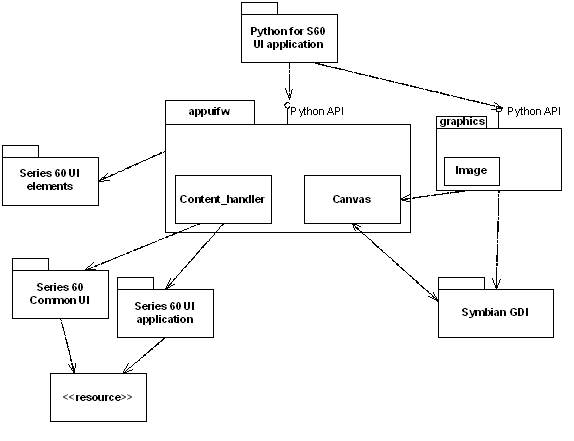
\includegraphics[width=\textwidth]{ui-overview}
\caption{Python for S60 UI environment overview}
\label{fig:ui-overview}
\end{figure}

\subsection{Basics of appuifw Module}
\label{subsec:basics}
Figure \ref{fig:normal-uilayout} shows the layout of a S60 application 
UI in the normal screen mode and a summary of how it relates to the services 
available at the \module{appuifw} API. For alternative layouts, see 
Figure \ref{fig:alternate-uilayouts}.

\begin{figure}
\centering
%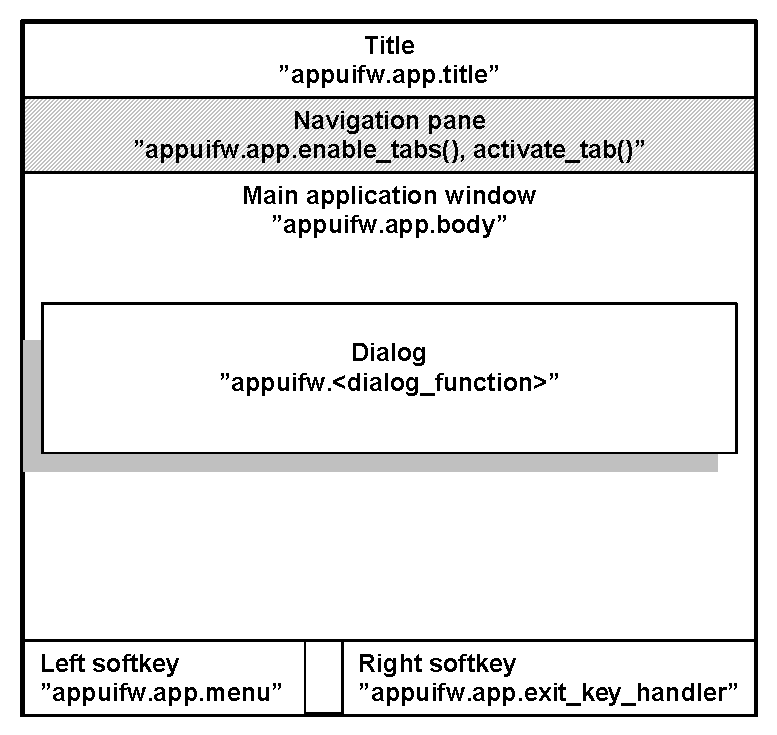
\includegraphics[width=0.7\textwidth]{screen-parts}
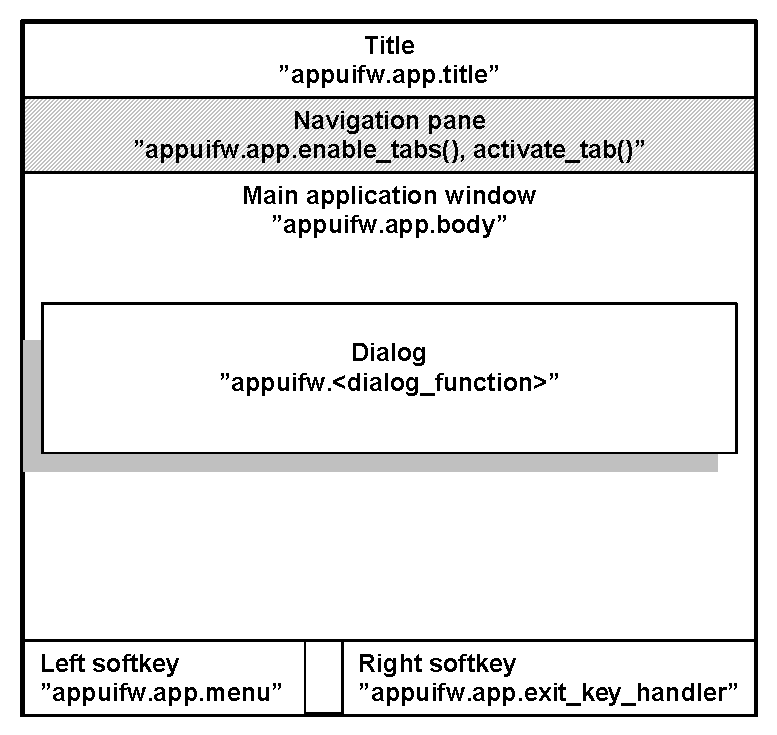
\includegraphics{screen-parts}
\caption{The different parts of the screen when using the 'normal' layout}
\label{fig:normal-uilayout}
\end{figure}

\begin{figure}
\centering
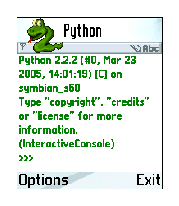
\includegraphics[width=\screenwidth]{layout-normal}
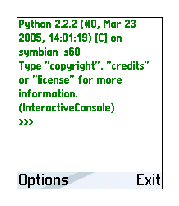
\includegraphics[width=\screenwidth]{layout-large}
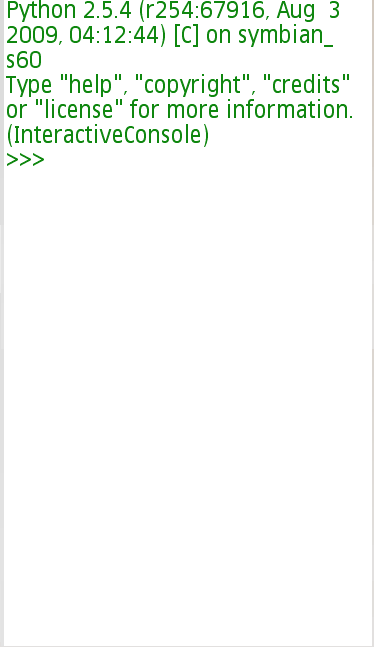
\includegraphics[width=\screenwidth]{layout-full}
\caption{UI layouts. left: 'normal', middle: 'large', right: 'full'}
\label{fig:alternate-uilayouts}
\end{figure}

The main application window may be set up to be occupied by a UI control.

A multi-view application can show the different views as tabs in the 
navigation pane and react as the users navigate between tabs. 

Dialogs always take precedence over the usual UI controls and appear on top 
of them.

UI controls are implemented as Python types. These types are available:

\begin{itemize}
\item \class{Text}
\item \class{Listbox}
\item \class{Canvas}
\end{itemize}
UI controls appear on the screen as soon as an instance of the corresponding 
Python type is set to the body field (\var{app.body}) of the current application UI.

\class{Form} is a versatile dialog implemented as a type.

The \class{Content_handler} type facilitates interfacing to other UI
applications and common high-level UI components. It is based on the
notion that designated handlers can reduce UI application interaction
to operations on MIME-type content.

The following dialogs are implemented as functions:

\begin{itemize}
\item \function{note}
\item \function{query}
\item \function{multi_query}
\item \function{selection_list}
\item \function{multi_selection_list}
\item \function{popup_menu}
\end{itemize}
A dialog becomes visible as soon as the corresponding Python function has 
been called. The function returns with the eventual user input or 
information on the cancellation of the dialog. \class{Form} is an 
exception; it is shown when its \method{execute} method is called.

\subsection{Softkeys}
\label{subsec:softkeys}
The softkeys are managed by the underlying S60 Platform. When no
dialog is visible, the right softkey is bound to application exit and
the left one represents an Options menu. Python for S60 offers
an interface for manipulating the menu and for binding the Exit key to
a Python-callable object (see Section \ref{subsec:application}). 

The native code that implements a dialog also manages the softkeys of the 
dialog, typically OK and Cancel. When the user input needs to be validated 
before accepting it and dismissing the dialog, it is best to use 
\class{Form}.

\subsection{Module Level Functions}
\label{subsec:module}
The following free functions - functions that do not belong to any class 
- are defined in the \module{appuifw} module:

\begin{funcdesc}{available_fonts}{}
Returns a list (Unicode) of all fonts available in the device.
\end{funcdesc}

\begin{funcdesc}{touch_enabled}{}
Returns 'True' if the device supports touch input, 'False' otherwise.
\end{funcdesc}

\begin{funcdesc}{query}{label, type\optional{, initial_value}}
Performs a query with a single-field dialog. The prompt is set to 
\var{label}, and the type of the dialog is defined by \var{type}. The 
value of \var{type} can be any of the following strings:

\begin{itemize}
\item \code{'text'}
\item \code{'code'}
\item \code{'number'}
\item \code{'date'}
\item \code{'time'}
\item \code{'query'}
\item \code{'float'}
\end{itemize}

The type of the optional \var{initial_value} parameter and the 
returned input depend on the value of \var{type}:

\begin{itemize}
\item For text fields, (\code{'text'}, \code{'code'}) it is Unicode
\item For number fields, it is numeric
\item For date fields, it is seconds since epoch rounded down to the nearest local midnight
\end{itemize}

A simple confirmation query and time query take no initial value and return 
\code{True/None} and seconds since local midnight, correspondingly. All 
queries return \code{None} if the users cancel the dialog. 

For \code{'float'} query the \var{initial_value} setting has no 
effect.
\end{funcdesc}


\begin{funcdesc}{multi_query}{label_1, label_2}
A two-field text (Unicode) input dialog. Returns the input values
as a 2-tuple. Returns \code{None} if the users cancel the dialog.
\end{funcdesc}

\begin{funcdesc}{note}{text\optional{, type\optional{, global}}}
Displays a note dialog of the chosen type with \var{text} 
(Unicode). The default value for \var{type} is \code{'info'}, which is 
automatically used if \var{type} is not set. \var{type} can be one of 
the following strings: \code{'error'}, \code{'info'} or 
\code{'conf'}. 

If \var{global} (integer) is any other value than zero a global note is 
displayed. A global note is displayed even if the Python application calling 
this function is in background. The same set of \var{type}s is supported as in 
standard note.
\end{funcdesc}

\begin{funcdesc}{popup_menu}{list\optional{, label}}
A pop-up menu style dialog. \var{list} representing the menu 
contents can be a list of Unicode strings or a list of Unicode string pairs 
(tuples). The resulting dialog list is then a single-style or a double-style 
list. A single-style list is shown in full; whereas a double-style list 
shows the items one at a time. Returns \code{None} if the user cancels the 
operation.
\end{funcdesc}

\begin{funcdesc}{selection_list}{choices\optional{, search_field=0}}
Executes a dialog that allows the users to select a list item and
returns the \var{index} of the chosen item, or \code{None} if the
selection is cancelled by the users. \var{choices} is a list of
Unicode strings.
\var{search_field} is \code{0} (disabled) by default and is optional. Setting it to \code{1} enables a search field (find pane) that facilitates searching for items in long lists. If enabled, the search field appears after you press a letter key.
\end{funcdesc}

\begin{funcdesc}{multi_selection_list}{choices\optional{, style='checkbox', search_field=0}}
  Executes a dialog that allows the users to select multiple list
  items.  Returns a tuple of indexes (a pair of Unicode strings) of
  the chosen items, or empty tuple if the no selection is made by
  the users. \var{choices} is a list of Unicode strings.  \var{style}
  is an optional string; the default value being \code{'checkbox'}.
  If \code{'checkbox'} is given, the list will be a checkbox list,
  where empty checkboxes indicate what items can be marked. The other
  possible value that can be set for \var{style} is
  \code{'checkmark'}. If \code{'checkmark'} is given, the list will be
  a markable list, which lists items but does not indicate
  specifically that items can be selected. To select items on a
  markable list, use the \var{'Options'} that has
  Mark/Unmark or the Edit key to select an item and the 
  Navigation key to browse the list. For example views on checkbox and
  markable lists, see
  \figurename~\ref{fig:checkbox-and-markable-list}.
  \var{search_field} is \code{0} (disabled) by default and is
  optional. Setting it to \code{1} enables a search field (find pane)
  that facilitates searching for items in long lists. If enabled, the
  search field is always visible with checkbox lists; with markable
  lists it appears by pressing a letter key.

Example:
\begin{verbatim}
tuple = appuifw.multi_selection_list([u'Harry', u'Ron', u'Hermione', u'Voldemort'], style='checkmark', search_field=1)
\end{verbatim}
\end{funcdesc}

\begin{figure}[htbp]
\centering
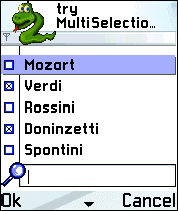
\includegraphics[width=\screenwidth]{checkbox-list}
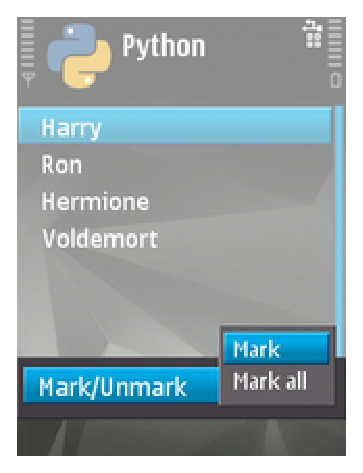
\includegraphics[width=\screenwidth]{markable-list}
\caption{Examples of a checkbox list (left) and a markable list (right)}
\label{fig:checkbox-and-markable-list}
\end{figure}

\subsection{Application Type}
\label{subsec:application}
A single implicit instance of this type always exists when \module{appuifw} 
module is present and can be referred to with the name \code{app}. New 
instances cannot be created by a Python program.

\begin{classdesc*}{Application}
Instances of \class{Application} type have the following attributes:

\begin{memberdesc}[Application]{body}
The UI control that is visible in the application's main window. Currently 
either \class{Text}, a \class{Listbox} object, \class{Canvas}, or 
\code{None}.
\end{memberdesc}

\begin{memberdesc}[Application]{directional_pad}
A boolean flag which controls the appearance of a virtual 4-way directional pad
that is displayed either at the bottom of the screen or on the right hand corner
depending on the orientation when using a Canvas. This is enabled by default on
devices that do not have a physical left and right soft key. This value is 
ignored on other devices, hence setting it to either True or False will have no effect.

Set it to \code{True} to enable 4-way directional pad and \code{False} to disable it.
\end{memberdesc}

\begin{memberdesc}[Application]{exit_key_handler}
A callable object that is called when the user presses the Exit softkey. 
Setting \member{exit_key_handler} to \code{None} sets it back to the 
default value.
\end{memberdesc}

\begin{memberdesc}[Application]{focus}
A callable object that is called with integer as parameter (0 = focus lost, 
1 = focus regained) when the application receives focus or it is switched to 
background. Focus is received e.g. when the application is switched from 
background to foreground or when the focus is regained from screensaver. 
Similarly when the screensaver is displayed, focus is lost.

Examples:
\begin{verbatim}
>>> import appuifw
>>> def cb(fg):
...   if(fg):
...     print "foreground"
...   else:
...     print "background"
...
>>> appuifw.app.focus=cb
>>> # switch to background, following text is printed from callback:
>>> background
>>> # switch to foreground, following text is printed from callback:
>>> foreground
\end{verbatim}

\begin{notice}
An improper callback can cause adverse effects. If you, for example,
define a callback which takes no parameters you will receive
never-ending \exception{TypeError} exceptions on the Nokia 6600.
\end{notice}

\end{memberdesc}

\begin{memberdesc}[Application]{menu}
This is a list of the following kinds of items:
\begin{itemize}
\item \code{(title, callback)} which creates a regular menu item
\item \code{(title, ((title, callback)\optional{...}))} which creates a submenu
\end{itemize}

\var{title} (Unicode) is the name of the item and \var{callback} the associated callable object. 
The maximum allowed number of items in a menu, or items in a submenu,
or submenus in a menu is 30.

Example:
\begin{verbatim}
appuifw.app.menu = [(u"Item 1", item1),
                    (u"Submenu 1", 
                        ((u"Subitem 1", subitem1),
                         (u"Subitem 2", subitem2)))]
\end{verbatim}
\end{memberdesc}

\begin{memberdesc}[Application]{orientation}
The orientation of the application. The orientation of the application can be 
one of the following values: \code{'automatic'} (this is the default value), 
\code{'portrait'} or \code{'landscape'}.
\end{memberdesc}

\begin{memberdesc}[Application]{screen}
The screen area used by an application. See \figurename~\ref{fig:alternate-uilayouts} for
example screens. The appearance of the application on the screen can
be affected by setting one of the following values: \code{'normal'},
\code{'large'} and \code{'full'}.

Examples:
\begin{verbatim}
appuifw.app.screen='normal'    # normal screen with title pane and softkey labels
appuifw.app.screen='large'     # only softkey labels visible
appuifw.app.screen='full'      # full screen mode on all devices
\end{verbatim}
\end{memberdesc}

\begin{memberdesc}[Application]{title}
The title of the application that is visible in the application's title
pane. Must be Unicode.
\end{memberdesc}

\begin{memberdesc}[Application]{track_allocations}
Set this to true if the interpreter should track all memory allocations and then
free the memory which was not explicitly released before application exit. The default
value of this attribute is true. As a consequence if there are any memory leaks in the
3rd party extension modules they will be released at the end. To check if there are
memory leaks(for debugging purposes) the following approach can be used :
\begin{verbatim}

appuifw.app.track_allocations = false

import my_extension
my_extension.do_something()

appuifw.app.track_allocations = true

\end{verbatim}
If the extension leaks memory then it will be reported at application exit.

\end{memberdesc}


Instances of \class{Application} type have the following methods:

\begin{methoddesc}[Application]{activate_tab}{index}
Activates the tab \var{index} counting from zero.
\end{methoddesc}

\begin{methoddesc}[Application]{full_name}{}
Returns the full name, in Unicode, of the native application in whose 
context the current Python interpreter session runs.
\end{methoddesc}

\begin{methoddesc}[Application]{layout}{layout_id}

Returns as a tuple the size and the position of the requested \code{layout_id}. 
The logical layouts are outlined partly in Figure \ref{fig:normal-uilayout}. The 
position is given from the top left corner. The \code{layout_id} can be one of 
the constants defined in module \module{appuifw}\footnote{Descriptions of the 
values are from the S60 SDK documentation \cite{S60Doc}.}:

\begin{datadesc}{EScreen} 
Screen.  
\end{datadesc}

\begin{datadesc}{EApplicationWindow} 
 Window that fills the entire screen.
\end{datadesc}

\begin{datadesc}{EStatusPane} 
Indicates common components for most of the applications.  
\end{datadesc}

\begin{datadesc}{EMainPane} 
The application main pane is used in all the applications.  
\end{datadesc}

\begin{datadesc}{EControlPane} 
Control pane.
\end{datadesc}

\begin{datadesc}{ESignalPane} 
The signal pane is used to indicate signal strength.  
\end{datadesc}

\begin{datadesc}{EContextPane} 
The context pane is used to indicate an active application.
\end{datadesc}

\begin{datadesc}{ETitlePane} 
Used to indicate the subject or the name of the main pane content. 
\end{datadesc}

\begin{datadesc}{EBatteryPane} 
The battery pane is used to indicate battery strength.  
\end{datadesc}

\begin{datadesc}{EUniversalIndicatorPane} 
The universal indicator pane is used to indicate items that require the user's 
attention while browsing applications. 
\end{datadesc}

\begin{datadesc}{ENaviPane} 
The navi pane is used to indicate navigation within an application, to provide 
context sensitive information to the user while entering or editing data, or to 
show additional information.  
\end{datadesc}

\begin{datadesc}{EFindPane} 
A fixed find pane is used with lists instead of the find pop-up window.  
\end{datadesc}

\begin{datadesc}{EWallpaperPane} 
Wallpaper pane.  
\end{datadesc}

\begin{datadesc}{EIndicatorPane} 
The universal indicator pane is used to indicate items that require the user's 
attention while browsing applications.  
\end{datadesc}

\begin{datadesc}{EAColumn} 
Used generally to display small sized graphics or heading texts.  
\end{datadesc}

\begin{datadesc}{EBColumn} 
Used generally to display large sized icons or heading texts.  
\end{datadesc}

\begin{datadesc}{ECColumn} 
Used generally to display data entered by the user. Overlaps with the D column. 
\end{datadesc}

\begin{datadesc}{EDColumn} 
Used generally to display additional icons. Overlaps with the C column. 
\end{datadesc}

\begin{datadesc}{EStaconTop} 
Top part of status and control panes in landscape layout.  
\end{datadesc}

\begin{datadesc}{EStaconBottom} 
Bottom part of status and control panes in landscape layout.  
\end{datadesc}

\begin{datadesc}{EStatusPaneBottom} 
Bottom part of status pane in landscape layout.  
\end{datadesc}

\begin{datadesc}{EControlPaneBottom} 
Bottom part of control pane in landscape layout.  
\end{datadesc}

\begin{datadesc}{EControlPaneTop} 
Top part of control pane in landscape layout.  
\end{datadesc}

\begin{datadesc}{EStatusPaneTop} 
Top part of status pane in landscape layout.
\end{datadesc}

Example:
\begin{verbatim}
>>> import appuifw
>>> appuifw.app.layout(appuifw.EMainPane)
((176, 144), (0, 44))
>>> # size and position (x, y) of the main pane in Nokia N70
\end{verbatim}

\end{methoddesc}

\begin{methoddesc}[Application]{set_exit}{}
Requests a graceful exit from the application as soon as the current script 
execution returns.
\end{methoddesc}

\begin{methoddesc}[Application]{set_tabs}{tab_texts\optional{,callback=None}}
Sets tabs with given names on them in the navigation bar; 
\var{tab_texts} is a list of Unicode strings. When the users 
navigate between tabs, \var{callback} gets called with the index 
of the active tab as an argument. Tabs can be disabled by giving an empty or 
one-item \var{tab_texts} list.
\end{methoddesc}

\begin{methoddesc}[Application]{uid}{}
Returns the UID, in Unicode, of the native application in whose 
context the current Python interpreter session runs.
\end{methoddesc}

\end{classdesc*}

\subsection{Form Type}
\label{subsec:form}
\class{Form} implements a dynamically configurable, editable multi-field 
dialog. \class{Form} caters for advanced dialog use cases with requirements 
such as free selectability of the combination of fields, possibility of 
validating the user input, and automatically producing the contents of some 
dialog fields before allowing the closing of the dialog. 

\begin{classdesc}{Form}{fields\optional{, flags=0}}
Creates a \class{Form} instance.
\var{fields} is a list of \emph{field descriptors}: \code{(label, type\optional{, value})} where

\var{label} is a Unicode string

\var{type} is one of the following strings: 
\code{'text'}, \code{'number'}, \code{'date'}, \code{'time'}, \code{'combo'}
or \code{'float'}

\var{value}, depending on \var{type}: Unicode string, numeric, float (seconds 
since Unix epoch rounded down to the nearest local midnight), float (seconds 
since local midnight), \code{([choice_label ...], index)} of float. For 
\code{'float'} \var{type} the initial value setting might not be shown in the 
UI.
\end{classdesc}

\class{Form} can also be configured and populated after construction. The 
configuration flags are visible as an attribute. \class{Form} implements 
the list protocol that can be used for setting the form fields, as well as 
obtaining their values after the dialog has been executed.

Instances of \class{Form} type have the following attributes:

\begin{memberdesc}[Form]{flags}
This attribute holds the values of the various configuration flags. 
Currently supported flags are:

\begin{datadesc}{FFormEditModeOnly}
When this flag is set, the form remains in edit mode while \method{execute} 
runs.
\end{datadesc}

\begin{datadesc}{FFormViewModeOnly}
When this flag is set, the form cannot be edited at all.
\end{datadesc}

\begin{datadesc}{FFormAutoLabelEdit}
This flag enables support for allowing the end-users to edit the labels of 
the form fields.
\end{datadesc}

\begin{datadesc}{FFormAutoFormEdit}
This flag enables automatic support for allowing the end-users to add and 
delete the form fields. Note that this is an experimental feature and is not 
guaranteed to work with all SDK versions.
\end{datadesc}

\begin{datadesc}{FFormDoubleSpaced}
When this flag is set, double-spaced layout is applied when the form is 
executed: one field takes two lines, as the label and the value field are on 
different lines.
\end{datadesc}
\end{memberdesc}

\begin{memberdesc}[Form]{menu}
A list of \code{(title, callback)} pairs, where 
each pair describes an item in the form's menu bar that is active while the 
dialog is being executed. \var{title} (Unicode) is the name of 
the item and \var{callback} the associated callable object.
\end{memberdesc}

\begin{memberdesc}[Form]{save_hook}
This attribute can be set to a callable object that receives one argument 
and returns a Boolean value. It gets called every time the users want to 
save the contents of an executing \class{Form} dialog. A candidate list for 
new form content - a list representing the currently visible state of the 
UI - is given as an argument. The list can be modified by 
\member{save_hook}. If \member{save_hook} returns \code{True}, the 
candidate list is set as the new contents of the form. Otherwise, the form 
UI is reset to reflect the field list contained in \class{Form} object.
\end{memberdesc}

Instances of \class{Form} type have the following methods:

\begin{methoddesc}[Form]{execute}{}
Executes the dialog by making it visible on the UI.
\end{methoddesc}

\begin{methoddesc}[Form]{insert}{index, field_descriptor}
Inserts the field descriptor into the \class{Form} before the given \var{index}.
\end{methoddesc}

\begin{methoddesc}[Form]{pop}{}
Removes the last field descriptor from the \class{Form} and returns it.
\end{methoddesc}

\begin{methoddesc}[Form]{length}{}the number of field descriptors in the form.
\end{methoddesc}

The subscript notation \code{f[i]} can be used to access or modify the
i-th element of the form \code{f}. Same limitations as discussed above
in the context of the flag \constant{FFormAutoFormEdit} apply to
modifying a form while it is executing. The ability to change the
schema of a form while it is executing is an experimental feature.

\subsection{Text Type}
\label{subsec:mylabel5}
\class{Text} is a text editor UI control. For examples on the options 
available with \class{Text}, see Figure \ref{fig:text-styles}.

\begin{figure}[htbp]
\centering
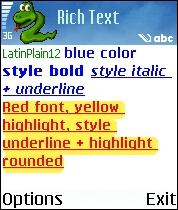
\includegraphics[width=\screenwidth]{text-styles-1}
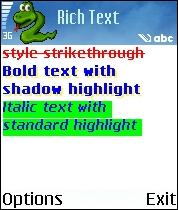
\includegraphics[width=\screenwidth]{text-styles-2}
\caption{Examples of the options available for Text type}
\label{fig:text-styles}
\end{figure}

Instances of \class{Text} type have the following attributes:

\begin{memberdesc}[Text]{color}
The color of the text. \code{color} supports the same color representation 
models as the \module{graphics} module. For the supported color 
representation models, see Section \ref{sec:graphics}.
\end{memberdesc}

\begin{memberdesc}[Text]{focus}
A Boolean attribute that indicates the focus state of the control. Editor 
control also takes the ownership of the navigation bar, and this feature is 
needed to enable the usage of this control in applications that use the 
navigation bar - for example, navigation tabs.
\end{memberdesc}

\begin{memberdesc}[Text]{font} 
The font of the text. There are two possible ways to set this attribute:

\begin{itemize}

\item Using a supported Unicode font, for example \code{u"Latin12"}. Trying to set a font which is not supported by the device has no effect. A list of supported fonts can be retrieved by using \function{appuifw.available_fonts}.

Example, setting font:
\begin{verbatim}
t = appuifw.Text()
t.font = u"albi17b" # sets font to Albi 17 bold
t.font = u"LatinPlain12" # sets font to Latin Plain 12
\end{verbatim}
\item Using one of the default device fonts that are associated with the following labels (plain strings):
\code{'annotation', 'title', 'legend', 'symbol', 'dense', 'normal'.}

Example, setting font: 
\begin{verbatim}
t.font = "title" # sets font to the one used in titles
\end{verbatim}

Example, checking the currently set font: 
\begin{verbatim}
unicodeFont = t.font
\end{verbatim}
\end{itemize}

The attribute value retrieved is always a Unicode string. If the font has 
been set with a label, for example, \code{'title'}, the attribute will 
retrieve the font associated with that label. 
\end{memberdesc}

\begin{memberdesc}[Text]{highlight_color}
The highlight color of the text. \code{highlight_color} supports the 
same color representation models as the \module{graphics} module. For the 
supported color representation models, see Section \ref{sec:graphics}.
\end{memberdesc}

\begin{memberdesc}[Text]{style}
The style of the text. The flags for this attribute are defined in the 
\module{appuifw} module. These flags can be combined by using the binary 
operator \code{|}. The flags can be divided into two types: text style 
and text highlight. Text style flags can be freely combined with each other. 
However, one or more text style flags can be combined with only one text 
highlight flag. The flags are:

Text style:

\begin{datadesc}{STYLE_BOLD} 
Enables bold text.
\end{datadesc}

\begin{datadesc}{STYLE_UNDERLINE}
Enables underlined text.
\end{datadesc}

\begin{datadesc}{STYLE_ITALIC} 
Enables italic text.
\end{datadesc}

\begin{datadesc}{STYLE_STRIKETHROUGH } 
Enables strikethrough.
\end{datadesc}

Text highlight:

\begin{datadesc}{HIGHLIGHT_STANDARD}
Enables standard highlight.
\end{datadesc}

\begin{datadesc}{HIGHLIGHT_ROUNDED}
Enables rounded highlight.
\end{datadesc}

\begin{datadesc}{HIGHLIGHT_SHADOW}
Enables shadow highlight.
\end{datadesc}

Only one highlight is allowed to be used at once. Therefore, it is possible 
to combine only one highlight with one or more text styles.

Examples:
\begin{verbatim}
t = appuifw.Text()

# These and other similar values and combinations are valid:
t.style = appuifw.STYLE_BOLD
t.style = appuifw.STYLE_UNDERLINE
t.style = appuifw.STYLE_ITALIC
t.style = appuifw.STYLE_STRIKETHROUGH
t.style = (appuifw.STYLE_BOLD|
	   appuifw.STYLE_ITALIC|
	   appuifw.STYLE_UNDERLINE)

# These values are valid:
t.style = appuifw.HIGHLIGHT_STANDARD
t.style = appuifw.HIGHLIGHT_ROUNDED
t.style = appuifw.HIGHLIGHT_SHADOW

# This combination is NOT valid:
# Invalid code, do not try!
t.style = (appuifw.HIGHLIGHT_SHADOW|appuifw.HIGHLIGHT_ROUNDED)
\end{verbatim}
\end{memberdesc}

Instances of \class{Text} type have the following methods:

\begin{methoddesc}[Text]{add}{text}
Inserts the Unicode string \var{text} to the current cursor position.
\end{methoddesc}

\begin{methoddesc}[Text]{bind}{event_code, callback}
Binds the callable Python object \var{callback} to event
\var{event_code}. The key codes are defined in 
the \module{key_codes} library module. The call 
\code{bind(event_code, None)} clears an 
existing binding. In the current implementation the event is always
passed also to the underlying native UI control.
\end{methoddesc}

\begin{methoddesc}[Text]{clear}{}
Clears the editor.
\end{methoddesc}

\begin{methoddesc}[Text]{delete}{\optional{pos=0, length=len()}}
Deletes \var{length} characters of the text held by the editor control, 
starting from the position \var{pos}.
\end{methoddesc}

\begin{methoddesc}[Text]{get_pos}{}
Returns the current cursor position.
\end{methoddesc}

\begin{methoddesc}[Text]{len}{}
Returns the length of the text string held by the editor control.
\end{methoddesc}

\begin{methoddesc}[Text]{get}{\optional{pos=0, length=len()}}
Retrieves \code{length} characters of the text held by the editor control, 
starting from the position \var{pos}.
\end{methoddesc}

\begin{methoddesc}[Text]{set}{text}
Sets the text content of the editor control to Unicode string 
\var{text}.
\end{methoddesc}

\begin{methoddesc}[Text]{set_pos}{cursor_pos}
Sets the cursor to \var{cursor_pos}.
\end{methoddesc}

\subsection{Listbox Type}
\label{subsec:listbox}

\begin{figure}[htbp]
\centering
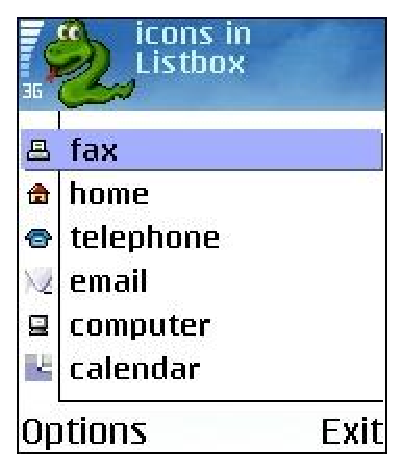
\includegraphics[width=\screenwidth]{listbox-with-icons}
\caption{Listbox with icons}
\label{fig:listbox-with-icons}
\end{figure}

An instance of this UI control type is visible as a listbox, also known as a 
list in Symbian, that can be configured to be a single-line item or a 
double-item listbox. Figure \ref{fig:listbox-with-icons} shows a single-line 
item Listbox with icons. For more information on the MBM and MIF formats, 
see Section \ref{subsec:icon}.

\begin{classdesc}{Listbox}{list, callback}
Creates a \class{Listbox} instance. A callable object 
\var{callback} gets called when a listbox selection has been 
made. \code{list} defines the content of the listbox and can be one of the 
following:

\begin{itemize}
\item A normal (single-line item) listbox: a list of Unicode strings, for example \code{[unicode_string item1, unicode_string item2]}
\item A double-item listbox: a two-element tuple of Unicode strings , for example \code{[(unicode_string item1, unicode_string item1description), (unicode_string item2, unicode_string item2description)]}
\item A normal (single-line item) listbox with graphics: a two-element tuple consisting of a Unicode string and an \class{Icon} object, for example \code{[(unicode_string item1, icon1), (unicode_string item2, icon2)]}.
\item A double-item listbox with graphics: a three-element tuple consisting of two Unicode strings and one \class{Icon} object, for example \code{[(unicode_string item1, unicode_string item1description, icon1), (unicode_string item2, unicode_string item2description, icon2)]}
\end{itemize}

Example: To produce a normal (single-line item) listbox with graphics:
\begin{verbatim}
icon1 = appuifw.Icon(u"z:\\resource\\apps\\avkon2.mbm", 28, 29)
icon2 = appuifw.Icon(u"z:\\resource\\apps\\avkon2.mbm", 40, 41)
entries = [(u"Signal", icon1),
           (u"Battery", icon2)]
lb = appuifw.Listbox(entries, lbox_observe)
\end{verbatim}
\end{classdesc}

\begin{notice}[note]
Known issue: Using this widget in large/full screen mode results in an unrefreshed area at the bottom of the screen.
\end{notice}

Instances of \class{Listbox} type have the following methods and properties:

\begin{methoddesc}[Listbox]{bind}{event_code, callback}
Binds the callable Python object \var{callback} to event 
\var{event_code}. The key codes are defined in 
the \module{key_codes} library module. The call
\code{bind(event_code, None)} clears an 
existing binding. In the current implementation the event is always passed 
also to the underlying native UI control.
\end{methoddesc}

\begin{methoddesc}[Listbox]{current}{}
Returns the currently selected item's index in the \class{Listbox}.
\end{methoddesc}

\begin{methoddesc}[Listbox]{set_list}{list\optional{, current}}
Sets the \class{Listbox} content to a list of Unicode strings or a
list of tuples of Unicode strings. The accepted structures of \var{list} are the
same as in the \class{Listbox} constructor. The optional argument \var{current} is the index of the focused list item.
\end{methoddesc}

\begin{memberdesc}[Listbox]{size}
The size of the \class{Listbox} as a tuple (width, height) - Read only.
\end{memberdesc}

\begin{memberdesc}[Listbox]{position}
The coordinates (as a tuple) of the top left corner of the \class{Listbox} -
Read only.
\end{memberdesc}

\subsection{Icon Type}
\label{subsec:icon}
An instance of \class{Icon} type encapsulates an icon to be used together 
with a \class{Listbox} instance. Note that currently \class{Icon} can only 
be used with \class{Listbox} (see Section \ref{subsec:listbox}).

MBM is the native Symbian OS format used for pictures. It is a
compressed file format where the files can contain several bitmaps and
can be referred to by a number. An \code{.mbg} file is the header file
usually associated with an \code{.mbm} file, which includes symbolic
definitions for each bitmap in the file. For example, an
\file{avkon.mbm} file has an associated index file called
\file{avkon.mbg}, which is included in S60 SDKs. For more information
on the MBM format and the bitmap converter tool, see \cite{S60Doc} and
search the topics with the key term "How to provide Icons"; this topic
also points you to the Bitmap Converter tool that can be used for
converting bitmaps into the MBM format.

\begin{classdesc}{Icon}{filename, bitmap, bitmapMask}
Creates an icon. \var{filename} is a Unicode file name and must 
include the whole path. Note that MBM is the only file formats supported.
\var{bitmap} and \var{bitmapMask} are integers that represent the index of 
the icon and icon mask inside that file respectively.
\end{classdesc}

Example: The following builds an icon with the standard signal symbol:
\begin{verbatim}
icon = appuifw.Icon(u"z:\\resource\\apps\\avkon2.mbm", 28, 29)
\end{verbatim}

\subsection{Content\_handler Type}
\label{subsec:content}

An instance of \class{Content_handler} handles data content by its MIME 
type.

\begin{classdesc}{Content_handler}{\optional{callback}}
Creates a \class{Content_handler} instance. A Content_handler handles
data content by its MIME type. The optional
\var{callback} is called when the embedded handler application 
started with the \method{open} method finishes. 
\end{classdesc}

Instances of \class{Content_handler} type have the following methods:

\begin{methoddesc}[Content_handler]{open}{filename}
Opens the file \var{filename} (Unicode) in its handler 
application if one has been registered for the particular MIME type. The 
handler application is embedded in the caller's thread. The call to this 
function returns immediately. When the handler application finishes, the 
\var{callback} that was given to the \class{Content_handler} 
constructor is called.
\end{methoddesc}

\begin{methoddesc}[Content_handler]{open_standalone}{filename}
Opens the file \var{filename} (Unicode) in its handler 
application if one has been registered for the particular MIME type. The 
handler application is started in its own process. The call to this function 
returns immediately. Note that \var{callback} is not called for 
applications started with this method.
\end{methoddesc}

\subsection{Canvas Type}
\label{subsec:canvas}
\class{Canvas} is a UI control that provides a drawable area on the screen 
and support for handling raw key events. \class{Canvas} supports the 
standard drawing methods that are documented in Section \ref{sec:graphics}.

\begin{classdesc}{Canvas}{\optional{redraw_callback=None, event_callback=None,
                                  resize_callback=None}}
Constructs a \class{Canvas}. The optional parameters are callbacks
that are called when specific events occur. 

\note{Watch out for cyclic
references here. For example, if the callbacks are methods of an
object that holds a reference to the \class{Canvas}, a reference cycle
is formed that must be broken at cleanup time or the
\class{Canvas} will not be freed.}

\var{redraw_callback} is called whenever a part of the \class{Canvas} 
has been obscured by something, is then revealed, and needs to be
redrawn. This can typically happen, for example, when the user
switches away from the Python application and back again, or after
displaying a pop-up menu. The callback takes as its argument a
four-element tuple that contains the top-left and the bottom-right
corner of the area that needs to be redrawn. In many cases redrawing
the whole
\class{Canvas} is a reasonable option. 

\var{event_callback} is called whenever a raw key event is received or when a 
pointer event occurs(only on touch input supported devices).
There are three kinds of key events: \code{EEventKeyDown},
\code{EEventKey}, and \code{EEventKeyUp}. When a user presses a key 
down, events \code{EEventKeyDown} and \code{EEventKey} are generated. 
When the key is released, an \code{EEventKeyUp} event is generated.

Pointer events are generated by touch input supported devices. When the screen
is touched the \code{EButton1Down} event is generated, \code{EDrag} while the
finger/stylus is dragged across the screen and then \code{EButton1Up} when the
finger/stylus is lifted.

The argument to the \var{event_callback} is a dictionary that contains 
the following data:

For key events:
\begin{itemize}
\item \code{'type'}: one of \code{EEventKeyDown}, \code{EEventKey}, or 
\code{EEventKeyUp}
\item \code{'keycode'}: the keycode of the key
\item \code{'scancode'}: the scancode of the key
\item \code{'modifiers'}: the modifiers that apply to this key event
\end{itemize}

For pointer events:
\begin{itemize}
\item \code{'type'}: one of the several pointer events - \code{EButton1Up}, 
\code{EButton1Down}, \code{EDrag} etc..
\item \code{'modifiers'}: the modifiers that apply to this pointer event
\item \code{'pos'}: A tuple containing the x-y pointer co-ordinates
\end{itemize}

Each key on the keyboard has one or more scancodes and zero or more keycodes 
associated with it. A scancode represents the physical key itself and a 
keycode is the result of state-related operating system defined processing 
done on the key. For keys that correspond to a symbol in the current 
character set of the phone, the keycode is equal to the code of the 
corresponding symbol in that character set. For example, if you are using 
the Nokia Wireless Keyboard (SU-8W), pressing the key A will always produce 
the scancode 65 (ASCII code for an upper case A), but the keycode 
could be either 65 or 91 (ASCII code for a lower case A) depending on 
whether or not the Shift key is pressed or Caps Lock is active. 

The \module{key_codes} module contains definitions for the keycodes and 
scancodes. See \figurename~\ref{fig:keyboard} for the codes of the most 
common keys on the phone keypad. 

Some keys are handled in a special way:

\begin{itemize}
\item A short press of the Edit key causes it to stay down, meaning that no \code{EEventKeyUp} event is sent. The event is only sent after a long press.
\item Detecting presses of the Voice tags key or the Power key is not supported.
\item If the right softkey is pressed, the \code{appuifw.app.exit_key_handler} callback is always executed.
\end{itemize}

There is no way to prevent the standard action of the Hang-up key, the Menu 
key, the Power key or the Voice tags key from taking place.

\begin{figure}
\centering
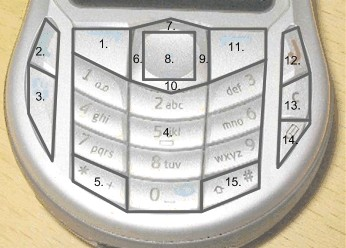
\includegraphics[width=5in]{6630keyboard}
%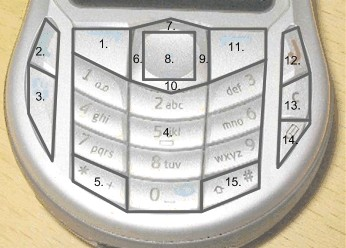
\includegraphics[width=3.60in,height=2.58in]{6630keyboard}
%\centerline{\includegraphics[width=3.60in,height=2.58in]{API_Reference_for_Python11.eps}} \par & 
\begin{tableiii}{lll}{textrm}{Key}{Keycode}{Scancode}
\lineiii{1.}{EKeyLeftSoftkey}{EScancodeLeftSoftkey}
\lineiii{2.}{EKeyYes}{EScancodeYes}
\lineiii{3.}{EKeyMenu}{EScancodeMenu}
\lineiii{4.}{EKey0...9}{EScancode0...9}
\lineiii{5.}{EKeyStar}{EScancodeStar}
\lineiii{6.}{EKeyLeftArrow}{EScancodeLeftArrow}
\lineiii{7.}{EKeyUpArrow}{EScancodeUpArrow}
\lineiii{8.}{EKeySelect}{EScancodeSelect}
\lineiii{9.}{EKeyRightArrow}{EScancodeRightArrow}
\lineiii{10.}{EKeyDownArrow}{EScancodeDownArrow}
\lineiii{11.}{EKeyRightSoftkey}{EScancodeRightSoftkey}
\lineiii{12.}{EKeyNo}{EScancodeNo}
\lineiii{13.}{EKeyBackspace}{EScancodeBackspace}
\lineiii{14.}{EKeyEdit}{EScancodeEdit}
\lineiii{15.}{EKeyHash}{EScancodeHash}
\end{tableiii}
\caption{Keycodes and scancodes for phone keys usable from Python applications}
\label{fig:keyboard}
\end{figure}

\var{resize_callback} is called when screen size is changed when the 
\class{Canvas} rect size has been changed. The callback takes as its argument a
two-element tuple that contains the new clientRect width and height. 

\end{classdesc}

Instances of \class{Canvas} type have the following methods:

\begin{methoddesc}[Canvas]{bind}{pointer_event, callable\optional{, ((x1, y1), (x2, y2))}}
This method can be used to listen to specific pointer events. The
\var{pointer_event} argument can be any one of the pointer events listed in the
\module{key_codes} module.

The most common pointer events are:

\begin{itemize}
\item \code{EButton1Down} - Pen down event 
\item \code{EButton1Up}   - Pen up event
\item \code{EDrag}        - Drag event (This event is only received when button1 is down)
\item \code{ESwitchOn}    - Switch on event caused by a screen tap.
\end{itemize}

\var{callable} is called when the pointer_event and the co-ordinate 
(if specified) criterion matches.

\var{((x1, y1), (x2, y2))} is an optional argument that can be passed to
specify the screen area to monitor for any specific pointer event. The two
co-ordinate tuple corresponds to the top-left and bottom-right points. This
argument will be ignored if the event is not a pointer event.

There are several ways in which bind can be used:

\begin{itemize}
\item \code{my_canv.bind(EButton1Up, callback)} - The callback is called when
EButton1Up event is generated anywhere in the canvas.

\item \code{my_canv.bind(EButton1Up, green_callback, ((x1, y1), (x2, y2)))} - The 
callback is called when the EButton1Up pointer event occurs inside the screen
area specified.

\item \code{my_canv.bind(EButton1Up, yellow_callback, ((x3, y3), (x4, y4)))} - 
Registers another callback for a different region but for the same pointer
event. When two screen areas overlap, the callback registered last will be
called when pointer events occur in the intersected region. 

\item \code{my_canv.bind(EButton1Up, callback3, ((x1, y1), (x2, y2)))} - If the
pointer event and the screen area to be monitored are the same, the callback
passed will replace the old callback already registered. 

\item \code{my_canv.bind(EButton1Up, None, ((x1, y1), (x2, y2)))} - If the pointer
event and the screen area to be monitored are the same, and the callback passed
is None, the callback registered previously is cleared.

\item \code{my_canv.bind(EButton1Up, None)} - All callbacks previously registered
for this pointer event are cleared, regardless of whether it was for a specific
screen area or for the entire canvas.
\end{itemize}

\begin{figure}
\centering
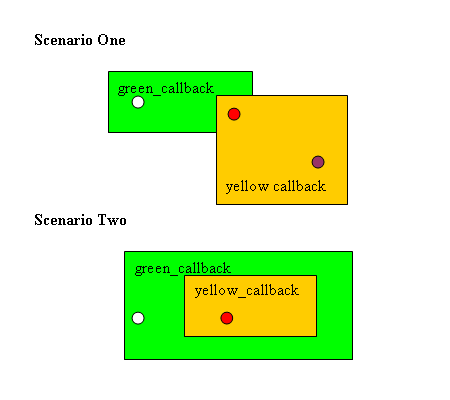
\includegraphics[width=5in]{bind-scenarios}
\caption{Canvas bind scenarios}
\label{fig:bind-scenarios}
\end{figure}

Clicking on the white spot should result in \code{green_callback} to be called. 
Clicking on the red spot should result in \code{yellow_callback} to be called in both
the scenarios shown above provided the \code{yellow_callback} was registered last. 
Clicking on the purple spot should result in \code{yellow_callback} to be called.

\end{methoddesc}

\begin{methoddesc}[Canvas]{begin_redraw}{\optional{((x1, y1), (x2, y2))}}
This is an explicit function that can be used to signal the window server that 
"I'm about to redraw this area". This method tells the window server that the 
window is about to respond to the last redraw event by redrawing the specified 
rectangle. This causes the window server to clear the rectangle, and remove it 
from the invalid region.
The optional co-ordinates x1, y1, x2, y2 should be the rectangle that has to be marked
for redrawing.

After the redraw is complete the application should call end_redraw().

\note{The begin_redraw and end_redraw methods should not be called inside the
redraw callback function.}

Couple of FAQs on redraw/non-redraw drawing:

Question: What is non-redraw drawing?
\begin{itemize}
\item "Non-redraw drawing" is any canvas/graphics drawing operation performed 
outside of begin_redraw()/end_redraw().
\end{itemize}

Question: What should applications do instead of non-redraw drawing?
\begin{itemize}
\item "Redraw drawing" is any drawing delimited by begin_redraw()/end_redraw().
\end{itemize}

Question: Why is non-redraw drawing bad for performance?
\begin{itemize}
\item The window server caches drawing operations in the redraw store.
Delimiting drawing with begin_redraw()/end_redraw() allows window server to 
efficiently manage drawing operations. 

If applications perform drawing operations outside begin_redraw/end_redraw,
window server cannot cull drawing operations from its cache of drawing 
operations, because it cannot know whether a set of drawing operations has 
been superceded by a new set.
In this scenario every frame of drawing that is done on a non-redraw drawing window 
will become slower and slower as it draws all the drawing operations for the 
entire history of the window (well actually up until the last begin_redraw/end_redraw 
for the whole window).

If an application performs begin_redraw/end_redraw, it tells the window server 
that it can throw away any old drawing operations it had for the area of the 
window specified in the redraw, thus allowing for more optimal management of 
drawing operations.
\end{itemize}

Question: What are the changes required for redraw drawing?
\begin{itemize}
\item Applications should delimit their drawing with begin_redraw()/end_redraw() 
- i.e. they should replace non-redraw drawing with redraw drawing. Sometimes, 
this is as straight forward as adding these calls to existing rendering code.
In other cases (where the application has been drawing using "incremental updates" 
to the window, the application drawing code would need to be reworked to perform a 
full refresh of the area redrawn for the rect provided in begin_redraw(rect).
\end{itemize}
\end{methoddesc}

\begin{methoddesc}[Canvas]{end_redraw}{}
Ends the current redraw. This function should be called when redrawing is complete.
\end{methoddesc}


Instances of \class{Canvas} type have the following attribute:

\begin{memberdesc}[Canvas]{size}
A two-element tuple that contains the current width and height of the 
\class{Canvas} as integers.
\end{memberdesc}

Instances of \class{Canvas} type have the same standard drawing methods 
that are documented in Section \ref{sec:graphics}.

\subsection{InfoPopup Type}
\label{subsec:infopopup}

An instance of \class{InfoPopup} type encapsulates an UI tip widget. This widget 
can be placed on top of other widgets to provide e.g. usage information to the 
user. The widget disappears as soon as the device's user presses any key or when 
the timer behind the \class{InfoPopup} is triggered.

\begin{classdesc}{InfoPopup}{}
Creates an \class{InfoPopup}.
\end{classdesc}

\begin{methoddesc}[InfoPopup]{show}{text, \optional{(x_coord, y_coord), 
time_shown, time_before, alignment}}
Show \var{text} (Unicode) in the \class{InfoPopup}. The optional parameters are 
the location (a tuple from the upper left corner), the time the popup is 
visible, \var{time_shown} (in milliseconds), the time before the popup, 
\var{time_before} (in milliseconds) and the alignment of the popup.

The default values are: the coordinates \code{(0, 0)}, \var{time_shown} 5 
seconds, \var{time_before} 0 seconds and for the alignment 
\code{appuifw.EHLeftVTop}.

The \var{alignment} can be one of the constants defined in module 
\code{appuifw}\footnote{Descriptions of the values are from the S60 SDK 
documentation \cite{S60Doc}.}:

\begin{datadesc}{EHLeftVTop} 
Object is left and top aligned. 
\end{datadesc}

\begin{datadesc}{EHLeftVCenter} 
Object is left aligned and centred vertically. 
\end{datadesc}

\begin{datadesc}{EHLeftVBottom} 
Object is left aligned and at the bottom. 
\end{datadesc}

\begin{datadesc}{EHCenterVTop} 
Object is centre aligned horizontally and at the top. 
\end{datadesc}

\begin{datadesc}{EHCenterVCenter} 
Object is centred horizontally and vertically. 
\end{datadesc}

\begin{datadesc}{EHCenterVBottom} 
Object is centred horizontally and at the bottom. 
\end{datadesc}

\begin{datadesc}{EHRightVTop} 
Object is right and top aligned. 
\end{datadesc}
 
\begin{datadesc}{EHRightVCenter} 
Object is right aligned and centred vertically. 
\end{datadesc}

\begin{datadesc}{EHRightVBottom} 
Object is right aligned and at the bottom. 
\end{datadesc}

\end{methoddesc}

\begin{methoddesc}[InfoPopup]{hide}{}
Hides the popup immediately.
\end{methoddesc}

Example:

\begin{verbatim}
>>> import appuifw
>>> i=appuifw.InfoPopup()
>>> i.show(u"Here is the tip.", (0, 0), 5000, 0, appuifw.EHRightVCenter)
>>>
\end{verbatim}

% Copyright (c) 2008-2009 Nokia Corporation
%
% Licensed under the Apache License, Version 2.0 (the "License");
% you may not use this file except in compliance with the License.
% You may obtain a copy of the License at
%
%     http://www.apache.org/licenses/LICENSE-2.0
%
% Unless required by applicable law or agreed to in writing, software
% distributed under the License is distributed on an "AS IS" BASIS,
% WITHOUT WARRANTIES OR CONDITIONS OF ANY KIND, either express or implied.
% See the License for the specific language governing permissions and
% limitations under the License.

\section{\module{globalui} --- 
    Interface to the S60 global UI notifiers }
\label{sec:globalui}

\declaremodule{extension}{globalui}
\platform{S60}
\modulesynopsis{Interface to the S60 global UI notifiers.}

The \module{globalui} module offers an interface to the S60 global UI notifiers. 
This allows a global note and query to be launched from an application which does not 
have a UI environment. 
The \module{globalui} module have functions:

\begin{funcdesc}{global_note}{note_text\optional{, type}}
Displays a note of the chosen type with \var{note_text} 
(Unicode). The default value for \var{type} is \code{'info'}. \var{type} can be 
one of the following strings: \code{'error'}, \code{'text'}, \code{'warn'}, \code{'charging'},
\code{'wait'}, \code{'perm'},\code{'not_charging'}, \code{'battery_full'}, \code{'battery_low'}, 
\code{'recharge_battery'}, or \code{'confirm'}. 
\end{funcdesc}

\begin{funcdesc}{global_query}{query_text\optional{, timeout}}
Displays a global confirmation query with \var{query_text} (Unicode). Returns 
\code{1} when the user presses 'Yes' and \code{0} otherwise. If the user does 
not respond to the query within \var{timeout} seconds, returns \code{None}. 
If the \var{timeout} value is 0, then the query waits indefinitely for user input. 
The default value for \var{timeout} is 0. The \var{timeout} value should be an integer.
\end{funcdesc}

\begin{funcdesc}{global_msg_query}{query_text, header_text\optional{, timeout}}
Displays a global message query with \var{query_text}(Unicode). \var{header_text} is used 
to set the heading string of the query. Returns \code{1} when the user 
presses 'OK' and \code{0} otherwise. If the user does not respond to the query within 
\var{timeout} seconds, returns \code{None}. If the \var{timeout} value is \code{0}, then the query 
waits indefinitely for user input. The default value for \var{timeout} is \code{0}. 
The \var{timeout} value should be an integer.
\end{funcdesc}

\begin{funcdesc}{global_popup_menu}{option_items\optional{, header_text, timeout}} 
Displays a global menu with \var{option_items}(Unicode). \var{header_text} is used to set the 
heading string of the menu. If no value is passed for \var{header_text}, then the header will
not be displayed. Returns the index value of the selected item from the list. If the user does
not respond to the menu within \var{timeout} seconds, returns \code{None}. If the \var{timeout}
value is \code{0}, then the menu waits indefinitely for the input. The default value for \var{timeout} 
is \code{0}. The \var{timeout} value should be an integer.
\end{funcdesc}

Example:
\begin{verbatim}
>>> import globalui, time
...
>>> text_to_show = u"text for showing note"
>>> globalui.global_note(text_to_show,'error')
>>> time.sleep(6)
>>> globalui.global_note(text_to_show)
>>> time.sleep(6)
>>> result = globalui.global_query(u"do you want to continue ?")
>>> time.sleep(6)
>>> listresult = globalui.global_popup_menu([u"MenuItem1", u"MenuItem2"],u"Select item",5)
...   
\end{verbatim}

% Copyright (c) 2005-2009 Nokia Corporation
%
% Licensed under the Apache License, Version 2.0 (the "License");
% you may not use this file except in compliance with the License.
% You may obtain a copy of the License at
%
%     http://www.apache.org/licenses/LICENSE-2.0
%
% Unless required by applicable law or agreed to in writing, software
% distributed under the License is distributed on an "AS IS" BASIS,
% WITHOUT WARRANTIES OR CONDITIONS OF ANY KIND, either express or implied.
% See the License for the specific language governing permissions and
% limitations under the License.

\section{\module{graphics} ---
  A graphics related services package}
\label{sec:graphics}

\declaremodule{extension}{graphics}
\platform{S60}
\modulesynopsis{A graphics related services package.}

The \module{graphics} module provides access to the graphics primitives and 
image loading, saving, resizing, and transformation capabilities provided by 
the Symbian OS. 

The module is usable from both graphical Python applications and
background Python processes. However, background processes have some
restrictions, namely that plain string symbolic font names are not
supported in background processes since background processes have no
access to the UI framework (see also Section
\ref{subsubsec:font-specs}).

For an example on using this module, see \cite{PyS60Prog}.

\subsection{Module Level Functions}
\label{subsec:mylabel7}
The following free functions - functions that do not belong to any class 
- are defined in the \module{graphics} module:

\begin{funcdesc}{screenshot}{}
Takes a screen shot and returns the image in \class{Image} format.
\end{funcdesc}

\subsection{Image Class Static Methods}
\label{subsec:image}
The following \class{Image} class static methods are defined in the 
\module{graphics} module:

\begin{funcdesc}{Image.new}{size\optional{, mode='RGB16'}}
Creates and returns a new \class{Image} object with the given size and 
mode. \var{size} is a two-element tuple. \var{mode} specifies the 
color mode of the \class{Image} to be created. It can be one of the 
following:

\begin{itemize}
\item \code{'1'}: Black and white (1 bit per pixel)
\item \code{'L'}: 256 gray shades (8 bits per pixel)
\item \code{'RGB12'}: 4096 colors (12 bits per pixel)
\item \code{'RGB16'}: 65536 colors (16 bits per pixel)
\item \code{'RGB'}: 16.7 million colors (24 bits per pixel)
\end{itemize}
It will also set the image size in twips according to the density of the device's primary screen. 
\end{funcdesc}

\begin{funcdesc}{Image.open}{filename}
Returns a new \class{Image} object (mode \code{RGB16}) that contains the 
contents of the named file. The supported file formats are JPEG and PNG. The 
file format is automatically detected based on file contents. 
\var{filename} should be a full path name.
\end{funcdesc}

\begin{funcdesc}{Image.inspect}{filename}
Examines the given file and returns a dictionary of the attributes of the 
file. At present the dictionary contains only the image size in pixels as a 
two-element tuple, indexed by key \code{'size'}. 
\var{filename} should be a full path name.
\end{funcdesc}

\subsection{Image Objects}
\label{subsec:image-objects}
An \class{Image} object encapsulates an in-memory bitmap. 

Note on asynchronous methods: Methods \method{resize}, \method{transpose}, 
\method{save}, and \method{load} have an optional callback argument. If the 
callback is not given, the method call is synchronous; when the method
returns, the operation is complete or an exception has been raised. If
the callback is given, the method calls are asynchronous. If all
parameters are valid and the operation can start, the method call will
return immediately.  The actual computation then proceeds in the
background. When it is finished, the callback is called with an error
code as the argument. If the given code is \code{0}, the operation
completed without errors, otherwise an error occurred.

It is legal to use an unfinished image as a source in a blit operation; this 
will use the image data as it is at the moment the blit is made and may thus 
show an incomplete result.

\class{Image} objects have the following methods:

\begin{methoddesc}[Image]{resize}{newsize\optional{, callback=None, keepaspect=0}}
Returns a new image that contains a resized copy of this image. If 
\var{keepaspect} is set to \code{1}, the resize will maintain the 
aspect ratio of the image, otherwise the new image will be exactly the given 
size. 

If \var{callback} is given, the operation is asynchronous, and the 
returned image will be only partially complete until \var{callback} is 
called.
\end{methoddesc}

\begin{methoddesc}[Image]{transpose}{direction\optional{, callback=None}}
Creates a new image that contains a transformed copy of this image. The 
\var{direction} parameter can be one of the following:

\begin{itemize}
\item \code{FLIP_LEFT_RIGHT}: Flips the image horizontally, exchanging left and right edges.
\item \code{FLIP_TOP_BOTTOM}: Flips the image vertically, exchanging top and bottom edges.
\item \code{ROTATE_90}: Rotates the image 90 degrees counterclockwise.
\item \code{ROTATE_180}: Rotates the image 180 degrees.
\item \code{ROTATE_270}: Rotates the image 270 degrees counterclockwise.
\end{itemize}

If \var{callback} is given, the operation is asynchronous and the 
returned image will be only partially complete until \var{callback} is 
called.
\end{methoddesc}

\begin{methoddesc}[Image]{load}{filename\optional{, callback=None}}
Replaces the contents of this \class{Image} with the contents of the named 
file, while keeping the current image mode. This \class{Image} object must 
be of the same size as the file to be loaded.

If \var{callback} is given, the operation is asynchronous and the loaded 
image will be only partially complete until \var{callback} is called. 
\var{filename} should be a full path name.
\end{methoddesc}

\begin{methoddesc}[Image]{save}{filename\optional{,callback=None, format=None, quality=75, bpp=24, compression='default'}}
Saves the image into the given file. The supported formats are JPEG and PNG. 
If \var{format} is not given or is set to \code{None}, the format is 
determined based on the file name extension: \code{'.jpg'} or 
\code{'.jpeg'} are interpreted to be in JPEG format and \code{'.png'} to 
be in PNG format. \var{filename} should be a full path name.

When saving in JPEG format, the \var{quality} argument specifies the 
quality to be used and can range from 1 to 100. 

When saving in PNG format, the \var{bpp} argument specifies how many bits 
per pixel the resulting file should have, and \var{compression} specifies 
the compression level to be used. 

Valid values for \var{bpp} are:

\begin{itemize}
\item \code{1}: Black and white, 1 bit per pixel
\item \code{8}: 256 gray shades, 8 bits per pixel
\item \code{24}: 16.7 million colors, 24 bits per pixel
\end{itemize}

Valid values for \var{compression} are:

\begin{itemize}
\item \code{'best'}: The highest possible compression ratio, the slowest speed
\item \code{'fast'}: The fastest possible saving, moderate compression
\item \code{'no'}: No compression, very large file size
\item \code{'default'}: Default compression, a compromise between file size and speed 
\end{itemize}

If \var{callback} is given, the operation is asynchronous. When the 
saving is complete, the \var{callback} is called with the result code.
\end{methoddesc}


\begin{methoddesc}[Image]{stop}{}
Stops the current asynchronous operation, if any. If an asynchronous call is 
not in progress, this method has no effect.
\end{methoddesc}

\class{Image} objects have the following attributes:

\begin{memberdesc}[Image]{size}
A two-element tuple that contains the size of the \class{Image}. Read-only.
\end{memberdesc}

\begin{memberdesc}[Image]{twipsize}
A two-element tuple that contains the size of the \class{Image} in twips. Read/Write.
\end{memberdesc}

\subsection{Common Features of Drawable Objects}
\label{subsec:common}
Objects that represent a surface that can be drawn on support a set of 
common drawing methods, described in this section. At present there are two 
such objects: \class{Canvas} from the \refmodule{appuifw} module and 
\class{Image} from the \module{graphics} module. 

\subsubsection{Options}
\label{subsubsec:options}
Many of these methods support a set of standard options. This set of options 
is as follows:

\begin{itemize}
\item \var{outline}: The color to be used for drawing outlines of primitives and text. If \code{None}, the outlines of primitives are not drawn.
\item \var{fill}: The color to be used for filling the insides of primitives. If \code{None}, the insides of primitives are not drawn. If \var{pattern} is also specified, \var{fill} specifies the color to be used for areas where the pattern is white.
\item \var{width}: The line width to be used for drawing the outlines of primitives.
\item \var{pattern}: Specifies the pattern to be used for filling the insides of primitives. If given, this must be either \code{None} or a 1-bit (black and white) \class{Image}.
\end{itemize}

\subsubsection{Coordinate representation}
\label{subsubsec:coordinate}
The methods accept an ordered set of coordinates in the form of a coordinate 
sequence. Coordinates can be of type \code{int}, \code{long}, or 
\code{float}. A valid coordinate sequence is a non-empty sequence of 
either

\begin{itemize}
\item Alternating x and y coordinates. In this case the sequence length must be even, or
\item Sequences of two elements, that specify x and y coordinates.
\end{itemize}
Examples of valid coordinate sequences:

\begin{itemize}
\item \code{(1, 221L, 3, 4, 5.85, -3)}: A sequence of three coordinates
\item \code{[(1,221L),(3,4),[5.12,6])}: A sequence of three coordinates
\item \code{(1,5)}: A sequence of one coordinate
\item \code{[(1,5)]}: A sequence of one coordinate
\item \code{[[1,5]]}: A sequence of one coordinate
\end{itemize}

Examples of invalid coordinate sequences:

\textbf{Invalid code, do not use!}
\begin{itemize}
\item \code{[]}: An empty sequence
\item \code{(1,2,3)}: Odd number of elements in a flat sequence
\item \code{[(1,2),(3,4),None]}: Contains an invalid element
\item \code{([1,2],3,4)}: Mixing the flat and nested form is not allowed
\end{itemize}

\subsubsection{Color representation}
\label{subsubsec:color}
All methods that take color arguments accept the following two color 
representations:

\begin{itemize}
\item A three-element tuple of integers in the range from 0 to 255 inclusive, representing the red, green, and blue components of the color.
\item An integer of the form \code{0xrrggbb}, where \code{rr} is the red, \code{gg} the green, and \code{bb} the blue component of the color. 
\end{itemize}
For 12 and 16 bit color modes the color component values are simply 
truncated to the lower bit depth. For the 8-bit grayscale mode images the 
color is converted into grayscale using the formula \code{(2*r+5*g+b)/8}, rounded 
down to the nearest integer. For 1-bit black and white mode images the color 
is converted into black (0) or white (1) using the formula \code{(2*r+5*g+b)/1024}.

Examples of valid colors:

\begin{itemize}
\item \code{0xffff00}: Bright yellow
\item \code{0x004000}: Dark green
\item \code{(255,0,0)}: Bright red
\item \code{0}: Black
\item \code{255}: Bright blue
\item \code{(128,128,128)}: Medium gray
\end{itemize}

Examples of invalid colors:

\textbf{Invalid code, do not use!}
\begin{itemize}
\item \code{(0,0.5,0.9)}: Floats are not supported
\item \code{'{\#}ff80c0'}: The HTML color format is not supported
\item \code{(-1,0,1000)}: Out-of-range values
\item \code{(1,2)}: The sequence is too short
\item \code{[128,128,192]}: This is not a tuple
\end{itemize}

\subsubsection{Font specifications}
\label{subsubsec:font-specs}
A font can be specified in three ways: 
\begin{itemize}
\item None, meaning the default font
\item a Unicode string that represents a full font name, such as \code{u'LatinBold19'}
\item a plain string symbolic name that refers to a font setting currently specified by 
the UI framework
\item as a two or three element tuple, where 
\begin{itemize}
\item the first element is the font name (unicode or string) or None for default font
\item the second element is the font height in pixels or None for default size
\item the third (optional) element is the flags applied to the font or None for default options.
\end{itemize}
\end{itemize}

The flags are the following:
\begin{itemize}
\item \code{FONT_BOLD} bold
\item \code{FONT_ITALIC} italic
\item \code{FONT_SUBSCRIPT} subscript
\item \code{FONT_SUPERSCRIPT} superscript
\item \code{FONT_ANTIALIAS} forces the font to be antialiased
\item \code{FONT_NO_ANTIALIAS} forces the font to not be antialiased
\end{itemize}

You can combine the flags with the binary or operator ``|''. For
example, the flags setting \code{FONT_BOLD|FONT_ITALIC} will produce
text that is both bold and italic.

Note: Antialiasing support is only available for scalable fonts.

You can obtain a list of all available fonts with the 
\module{appuifw} module function \function{available_fonts}.

The symbolic names for UI fonts are:
\begin{itemize}
\item \code{'normal'}
\item \code{'dense'}
\item \code{'title'}
\item \code{'symbol'}
\item \code{'legend'}
\item \code{'annotation'}
\end{itemize}
Since background processes have no access to the UI framework, these 
symbolic names are not supported in them. You need to specify the full font 
name.

\subsubsection{Common Methods of Drawable Objects}
\label{subsubsec:common}
\begin{methoddesc}{line}{coordseq\optional{, $<$options$>$}}
Draws a line connecting the points in the given coordinate sequence. For 
more information about the choices available for \var{options}, 
see Section \ref{subsubsec:options}.
\end{methoddesc}

\begin{methoddesc}{polygon}{coordseq\optional{, $<$options$>$}}
Draws a line connecting the points in the given coordinate sequence, and 
additionally draws an extra line connecting the first and the last point in 
the sequence. If a fill color or pattern is specified, the polygon is filled 
with that color or pattern. For more information about the choices available 
for \var{options}, see Section \ref{subsubsec:options}.
\end{methoddesc}

\begin{methoddesc}{rectangle}{coordseq\optional{, $<$options$>$}}
Draws rectangles between pairs of coordinates in the given sequence. The 
coordinates specify the top-left and the bottom- right corners of the 
rectangle. The sequence must have an even number of coordinates. For more 
information about the choices available for \var{options}, see 
Section \ref{subsubsec:options}.
\end{methoddesc}

\begin{methoddesc}{ellipse}{coordseq\optional{, $<$options$>$}}
Draws ellipses between pairs of coordinates in the given sequence. The
coordinates specify the top-left and bottom-right corners of the
rectangle inside which the ellipse is contained.  The sequence must
have an even number of coordinates. 
For more information about the choices available for \var{options}, see 
Section \ref{subsubsec:options}.
\end{methoddesc}

\begin{methoddesc}{pieslice}{coordseq, start, end\optional{, $<$options$>$}}
Draws pie slices contained in ellipses between pairs of coordinates in
the given sequence. The start and end parameters are floats that
specify the start and end points of pie slice as the starting and
ending angle in radians. The angle \code{0} is to the right, the angle
\code{pi/2} is straight up, \code{pi} is to the left and\code{-pi/2}
is straight down. \var{coordseq} is interpreted the same way as for
the \method{ellipse} method.
For more 
information about the choices available for \var{options}, see 
Section \ref{subsubsec:options}.
\end{methoddesc}

\begin{methoddesc}{arc}{coordseq, start, end\optional{, $<$options$>$}}
Draws arcs contained in ellipses between pairs of coordinates in
the given sequence. The start and end parameters are floats that
specify the start and end points of pie slice as the starting and
ending angle in radians. The angle \code{0} is to the right, the angle
\code{pi/2} is straight up, \code{pi} is to the left and\code{-pi/2}
is straight down. \var{coordseq} is interpreted the same way as for
the \method{ellipse} method.  For more information about the choices
available for \var{options}, see Section
\ref{subsubsec:options}.
\end{methoddesc}

\begin{methoddesc}{point}{coordseq\optional{, $<$options$>$}}
Draws points in each coordinate in the given coordinate sequence. If the 
\var{width} option is set to greater than 1, draws a crude approximation 
of a circle filled with the outline color in the locations. Note that
the approximation is not very accurate for large widths; use the
\method{ellipse} method if you need a precisely formed circle. 
For more information about the choices
available for \var{options}, see Section
\ref{subsubsec:options}.
\end{methoddesc}

\begin{methoddesc}{clear}{\optional{color=0xffffff}}
Sets the entire surface of the drawable to the given color, white by 
default.
\end{methoddesc}

\begin{methoddesc}{text}{coordseq, text\optional{fill=0, font=None}}
Draws the given text in the points in the given coordinate sequence
with the given color (default value is black) and the given font. The
font specification format is described above.
\end{methoddesc}

\begin{methoddesc}{measure_text}{text\optional{font=None, maxwidth=-1, maxadvance=-1}}
Measures the size of the given text when drawn using the given
font. Optionally you can specify the maximum width of the text or the
maximum amount the graphics cursor is allowed to move (both in pixels).

Returns a tuple of three values: 
\begin{itemize}
\item the bounding box for the text as a 4-tuple: (topleft-x, topleft-y, bottomright-x, bottomright-y)
\item the number of pixels the graphics cursor would move to the right
\item the number of characters of the text that fits into the given maximum width and advance
\end{itemize}
\end{methoddesc}

\begin{methoddesc}{blit}{image\optional{,target=(0,0), source=((0,0),image.size), mask=None, scale=0}}
Copies the source area from the given \var{image} to the target area
in this drawable. The source area is copied in its entirety if
\var{mask} is not given or is set to \code{None}. If the mask is
given, the source area is copied where the mask is white. \var{mask}
can be either \code{None}, a 1-bit (black and white) \class{Image} or
a grayscale \class{Image}, and must be of the same size as the source image. A grayscale mask acts
as an alpha channel, i.e. partial transparency.

\var{target} and \var{source} specify the target area in this image 
and the source area in the given source. They are coordinate sequences of 
one or two coordinates. If they specify one coordinate, it is interpreted as 
the upper-left corner for the area; if they specify two coordinates, they 
are interpreted as the top-left and bottom-right corners of the area.

If \var{scale} is other than zero, scaling is performed on the fly while 
copying the source area to the target area. If \var{scale} is zero, no 
scaling is performed, and the size of the copied area is clipped to the 
smaller of source and target areas.

Note that a \method{blit} operation with scaling is slower than one without 
scaling. If you need to blit the same \class{Image} many times in a scaled 
form, consider making a temporary \class{Image} of the scaling result and 
blitting it without scaling. Note also that the scaling performed by the 
\method{blit} operation is much faster but of worse quality than the one 
done by the \method{resize} method, since the \method{blit} method does not 
perform any antialiasing.
\end{methoddesc}

% Copyright (c) 2005-2009 Nokia Corporation
%
% Licensed under the Apache License, Version 2.0 (the "License");
% you may not use this file except in compliance with the License.
% You may obtain a copy of the License at
%
%     http://www.apache.org/licenses/LICENSE-2.0
%
% Unless required by applicable law or agreed to in writing, software
% distributed under the License is distributed on an "AS IS" BASIS,
% WITHOUT WARRANTIES OR CONDITIONS OF ANY KIND, either express or implied.
% See the License for the specific language governing permissions and
% limitations under the License.

\section{\module{camera} ---
    Interface for taking photographs and video recording}

\declaremodule{extension}{camera}
\label{sec:camera}
\platform{S60}

The \module{camera} module enables taking photographs and video recording.

The following data items for state information are available in \module{camera}:

\begin{datadesc}{EOpenComplete}
The opening of the video clip has succeeded.
\end{datadesc}

\begin{datadesc}{ERecordComplete}
The video recording has completed (not called on explicit \code{stop_recording} 
call).
\end{datadesc}

\begin{datadesc}{EPrepareComplete}
The device is ready to begin video recording.
\end{datadesc}

The \module{camera} module has the following functions\footnote{Descriptions 
for some of the values are based on information found in S60 SDK documentation 
\cite{S60Doc}}:

\begin{funcdesc}{cameras_available}{}
Returns the number of cameras available in the device.
\end{funcdesc}

\begin{funcdesc}{image_modes}{}
Returns the image modes supported in the device as a list of strings, for 
example: \code{['RGB12', 'RGB', 'JPEG_Exif', 'RGB16'].}
\end{funcdesc}

\begin{funcdesc}{image_sizes}{}
Returns the image sizes (resolution) supported in the device as a list of 
\code{(x, y)} tuples, for example: \code{[(640, 480), (160, 120)]}.
\end{funcdesc}

\begin{funcdesc}{flash_modes}{}
Returns the flash modes available in the device as a list of strings. 
\end{funcdesc}

\begin{funcdesc}{max_zoom}{}
Returns the maximum digital zoom value supported in the device as an 
integer. 
\end{funcdesc}

\begin{funcdesc}{exposure_modes}{}
Returns the exposure settings supported in the device as a list of strings. 
\end{funcdesc}

\begin{funcdesc}{white_balance_modes}{}
Returns the white balance modes available in the device as a list of 
strings. 
\end{funcdesc}

\begin{funcdesc}{take_photo}{\optional{mode, size, zoom, flash, exposure, white_balance, position}}
Takes a photograph and returns the image in:

\begin{enumerate}
  \item \code{Image} format (for more information on \code{Image} format, see 
  Chapter \ref{sec:graphics} \refmodule{graphics} Module) or
  
  \item Raw JPEG data\footnote{For more information, see e.g. 
  \url{http://en.wikipedia.org/wiki/JPEG}.}. 
\end{enumerate}

The settings listed below describe all settings that are supported by the 
\code{camera} module. You can retrieve the mode settings available for your 
device by using the appropriate functions listed at the beginning of this 
chapter.

\begin{itemize}

\item \var{mode} is the display mode of the image. The default value is 
\code{'RGB16'}. The following display modes are supported for the \code{Image} 
format pictures taken:
	\begin{itemize}
	\item \code{'RGB12'}: 4096 colors (12 bits per pixel)
	\item \code{'RGB16'}: 65536 colors (16 bits per pixel). Default value, always supported
	\item \code{'RGB'}: 16.7 million colors (24 bits per pixel)
	\end{itemize}

For the JPEG data format images the following modes are supported:

	\begin{itemize}
	\item \code{'JPEG_Exif'}: JPEG Exchangeable image file format
	\item \code{'JPEG_JFIF'}: JPEG File Interchange Format
	\end{itemize}

Note that there is variety between the devices and the supported formats.

\item \var{size} is the resolution of the image. The default value is \code{(640, 480)}. The following sizes are supported, for example, in Nokia 6630: \code{(1280, 960)}, \code{(640, 480)} and \code{(160, 120)}.
\item \var{flash} is the flash mode setting. The default value is \code{'none'}. The following flash mode settings are supported:
	\begin{itemize}
	\item \code{'none' \newline
}No flash. Default value, always supported
	\item \code{'auto' \newline
}Flash will automatically fire when required
	\item \code{'forced' \newline
}Flash will always fire
	\item \code{'fill_in' \newline
}Reduced flash for general lighting
	\item \code{'red_eye_reduce' \newline
}Red-eye reduction mode
	\end{itemize}
\item \var{zoom} is the digital zoom factor. It is assumed to be on a linear scale from 0 to the maximum zoom value allowed in the device. The default value is \code{0}, meaning that zoom is not used. 
\item \var{exposure} is the exposure adjustment of the device. Exposure is a combination of lens aperture and shutter speed used in taking a photograph. The default value is \code{'auto'.} The following exposure modes are supported:
	\begin{itemize}
	\item \code{'auto'} \newline
Sets exposure automatically. Default value, always supported
	\item \code{'night'} \newline
Night-time setting for long exposures
	\item \code{'backlight' } \newline
Backlight setting for bright backgrounds
	\item \code{'center'} \newline
Centered mode for ignoring surroundings
	\end{itemize}
\item \var{white_balance} can be used to adjust white balance to match the main source of light. The term white balance refers to the color temperature of the current light. A digital camera requires a reference point to represent white. It will then calculate all the other colors based on this white point. The default value for \var{white_balance} is \code{'auto'} and the following white balance modes are supported:
	\begin{itemize}
	\item \code{'auto'} \newline
Sets white balance automatically. Default value, always supported
	\item \code{'daylight'} \newline
Sets white balance to normal daylight
	\item \code{'cloudy}' \newline
Sets white balance to overcast daylight
	\item \code{'tungsten'} \newline
Sets white balance to tungsten filament lighting
	\item \code{'fluorescent}' \newline
Sets white balance to fluorescent tube lighting
	\item \code{'flash'} \newline
Sets white balance to flash lighting
	\end{itemize}
\item \var{position} is the camera used if the device, such as Nokia N95, has several cameras. In Nokia N95, the camera pointing to the user of the device is located in position \code{1}, whereas the one pointing away from the user is located in position \code{0}. The default \var{position} is \code{0}.
\end{itemize}

If some other application is using the camera, this operation fails, with error 
\code{SymbianError: KErrInUse}. Invoking this function right after the device 
boot, might result in \code{SymbianError: KErrNotReady} error.

In some Nokia devices (e.g. in N95), to be able to get the highest possible size 
for the captured image, you need to:

\begin{enumerate}
\item switch to the landscape mode (see \code{appuifw.app.orientation})
\item import the \code{camera} module
\item take the picture in the \code{'JPEG_Exif'} format.
\end{enumerate}

\item

\end{funcdesc}

\begin{funcdesc}{start_finder}{callable\optional{, backlight_on=1, size=main_pane_size}}

Starts the camera viewfinder and binds a callback to receive \code{Image} format 
feed. When a new viewfinder frame is ready the callback is invoked with the 
\code{Image} as parameter.

The optional parameter \code{backlight_on} determines whether the device 
backlight is kept on when the camera view finder is in operation. By default, 
the backlight is on (1 = on, 0 = off).

The optional parameter \code{size} (of type tuple, e.g. \code{(176, 144)}) can 
be used to change the size of the \code{Image} received in the callback. The 
default \code{size} is the same as the application's main pane size. 

Example view finder code:

\begin{verbatim}
>>> import appuifw
>>> import camera
>>> def cb(im):
...   appuifw.app.body.blit(im)
...
>>> import graphics
>>> appuifw.app.body=appuifw.Canvas()
>>> camera.start_finder(cb)
>>>
\end{verbatim}

\end{funcdesc}

\begin{funcdesc}{stop_finder}{}
Stops the viewfinder.
\end{funcdesc}

\begin{funcdesc}{release}{}
Releases the camera -- After invocation other applications can access the camera 
hardware.
\end{funcdesc}

\begin{funcdesc}{start_record}{filename, callable}
Starts video recording. \var{filename} is the file where the video clip is saved 
and \var{callable} will be called with possible error code (int) and status 
information (see data in module \module{camera}) as parameter.

Prior calling this function, the view finder needs to be started.
\end{funcdesc}

\begin{funcdesc}{stop_record}{}
Stops the video recording.
\end{funcdesc}

% Copyright (c) 2006 - 2009 Nokia Corporation
%
% Licensed under the Apache License, Version 2.0 (the "License");
% you may not use this file except in compliance with the License.
% You may obtain a copy of the License at
%
%     http://www.apache.org/licenses/LICENSE-2.0
%
% Unless required by applicable law or agreed to in writing, software
% distributed under the License is distributed on an "AS IS" BASIS,
% WITHOUT WARRANTIES OR CONDITIONS OF ANY KIND, either express or implied.
% See the License for the specific language governing permissions and
% limitations under the License.

\section{\module{keycapture} ---
         Interface for global capturing of key events.}
\label{sec:keycapture}

\declaremodule{extension}{keycapture}		% not standard, in C
\platform{S60}
\modulesynopsis{Interface for global capturing of key events.}

The \module{keycapture} module offers an API for global capturing of key events. The 
\module{keycapture} module provides the \class{KeyCapturer} object as a tool for listening to 
events.

The \class{KeyCapturer} object uses a callback method to report the key 
events. The callback method is called each time any of the specified keys 
is pressed.

Currently the \module{keycapture} module does not support capturing separate key-up or
key-down events.

\begin{notice}[note]
Keycapture module requires SwEvent capability.
\end{notice}

\subsection{Module Level Constants}
The following constants are defined in the \module{keycapture} module:

\begin{datadesc}{all_keys}
A list of all key codes defined in the \module{key_codes} module.
\end{datadesc}

\subsection{KeyCapturer objects} 
\label{KeyCapturer objects}

\class{KeyCapturer} object takes a callback method as a mandatory parameter to 
its constructor. The callback method must have one single parameter for 
forwarding the key code of the captured key.

There can be several \class{KeyCapturer} objects existing at the same time.

\class{KeyCapturer} object has following methods and properties:

\begin{memberdesc}[KeyCapturer]{keys}
List of keys to be captured. Can be read and written.
\\Example:
\begin{verbatim}
keys = (key_codes.EkeyUpArrow,)
keys = keycapture.all_keys
\end{verbatim} 
\end{memberdesc}

\begin{memberdesc}[KeyCapturer]{forwarding}
Specifies whether captured key events are forwarded to other applications or not.
Either has value 1 or 0. Can be read and written.
\end{memberdesc}

\begin{methoddesc}[KeyCapturer]{start}{}
Starts the actual capturing of key events.
\end{methoddesc}

\begin{methoddesc}[KeyCapturer]{stop}{}
Stops the actual capturing of key events.
\end{methoddesc}

\begin{methoddesc}[KeyCapturer]{last_key}{}
Returns last key code that is captured. 
\end{methoddesc}

% Copyright (c) 2006-2009 Nokia Corporation
%
% Licensed under the Apache License, Version 2.0 (the "License");
% you may not use this file except in compliance with the License.
% You may obtain a copy of the License at
%
%     http://www.apache.org/licenses/LICENSE-2.0
%
% Unless required by applicable law or agreed to in writing, software
% distributed under the License is distributed on an "AS IS" BASIS,
% WITHOUT WARRANTIES OR CONDITIONS OF ANY KIND, either express or implied.
% See the License for the specific language governing permissions and
% limitations under the License.

\section{\module{topwindow} ---
         Interface for creating windows that are shown on top of other 
         applications.}
\label{sec:topwindow}

\declaremodule{extension}{topwindow}
\platform{S60}
\modulesynopsis{Interface for creating windows that are shown on top of other 
         applications.}
         
The \module{topwindow} module offers an API for creating windows that are shown 
on top of other applications and managing the content of these windows. 
Images can be inserted into the windows and the background color, visibility, 
corner type and shadow of the window can be manipulated.

\module{topwindow} extension does not provide sophisticated drawing capabilities 
by any means but rather relies on services provided by the \module{graphics} 
extension: \module{topwindow} allows \module{graphics} \class{Image} objects to 
be put into the windows that are represented by \class{TopWindow} objects.

\class{TopWindow} object provides mainly only two services: \class{TopWindow} 
objects can be shown or hidden and Images can be put into the windows. However, 
several images can be added into one \class{TopWindow} object and several 
\class{TopWindow} objects can be created and shown. Since the images can be 
manipulated using the \module{graphics} extension this makes it possible to 
create many kind of content to the \class{TopWindow} objects.

\subsection{TopWindow objects}

\begin{classdesc}{TopWindow}{}
Create a \class{TopWindow} object.
\end{classdesc}

\class{TopWindow} objects have the following methods and properties:

\begin{methoddesc}[TopWindow]{show}{}
Shows the window. The window is not shown until show() is called.
\end{methoddesc}

\begin{methoddesc}[TopWindow]{hide}{}
Hides the window.
\end{methoddesc}

\begin{methoddesc}[TopWindow]{add_image}{image, position}
Inserts an image object \class{graphics.Image} into the window. The position 
of the image is specified by the \var(position) parameter. 
If only the coordinates of the top left corner are specified, like (x1, y1) 
the image is not resized. If four coordinates are given, like(x1, y1, x2, y2), 
the image is resized to fit to the specified area.
\\Example:
\begin{verbatim} 
add_image(image, (10,20))
add_image(image, (10,20,20,30))
\end{verbatim}
\end{methoddesc}

\begin{methoddesc}[TopWindow]{remove_image}{image\optional{,position}}
Removes the image from the window.
Mandatory parameter \var{image} must be a \class{graphics.Image} object. 
Parameter \var{position} may specify the top-left corner coordinates of the 
image or the rectangular area of the image. If only \var{image} parameter is 
given, all the pictures representing this image object are removed from the
window. If both parameters are given, only the picture that matches both 
parameters is removed.
\\Example:
\begin{verbatim}
remove_image(image)
remove_image(image, (10,10))
remove_image(image, (10,10,20,20))
\end{verbatim}
\end{methoddesc}

\begin{memberdesc}[TopWindow]{position}
Specifies the coordinates of the top left corner of the window. Can be read and written.
\\Example: 
\begin{verbatim}
position = (10, 20)
\end{verbatim}
\end{memberdesc}

\begin{memberdesc}[TopWindow]{size}
Specifies the size of the window. Can be read and written.
\\Example:
\begin{verbatim} 
size = (100, 200)
\end{verbatim}
\end{memberdesc}

\begin{memberdesc}[TopWindow]{images}
The images inserted into the window. Defined as a list of tuple objects. Each 
tuple contains a \class{graphics.Image} object and the \var{position} of the 
image. The \var{position} may specify the top-left coordinate of the image and 
optionally also the bottom-right coordinate of the image. Parameter (x,y) 
specifies the top-left coordinate, but does not resize the image while 
parameter like (x1,y1,x2,y2) specifies both the top-left and bottom-right 
coordinates and possibly also resizes the image. Can be read and written.
Also see the \method{add_image()} and \method{remove_image()} methods.
\\Example: 
\begin{verbatim}
images = [(image1,(x1,y1)), (image2,(x1,y1,x2,y2)), (image3,(50,50,100,100))]
\end{verbatim}
sets the window content to be 3 images. \code{image2} and \code{image3} are possibly resized 
while the \code{image1} is not)
\end{memberdesc}

\begin{memberdesc}[TopWindow]{shadow}
Specifies if the shadow of the window is shown and the length of the shadow. 
Can be read and written. Setting \code{shadow = 0} makes the shadow invisible.
\\Example: 
\code{shadow = 5}
\end{memberdesc}

\begin{memberdesc}[TopWindow]{corner_type}
Specifies the corner type of the window. Can be read and written. Corner type 
can be one of the following values: 
\begin{itemize}
\item \code{square}
\item \code{corner1}
\item \code{corner2}
\item \code{corner3}
\item \code{corner5}
\end{itemize}

Example: 
\code{corner_type = "square"}
\end{memberdesc}

\begin{memberdesc}[TopWindow]{maximum_size}
Returns the maximum size of the window as a tuple (width, height). Read only 
property.
\end{memberdesc}

\begin{memberdesc}[TopWindow]{background_color}
The background color of the window as an integer (e.g. \code{0xaabbcc}). The two 
greatest hexadecimal digits specify the red, the next two specify the blue and 
the last ones specify the green color. Can be read and written.
\\Example: 
\code{background_color = 0xffffff} (sets the white color)
\end{memberdesc}

\begin{memberdesc}[TopWindow]{visible}
Can be set to 0 or 1. 1 means that window is visible, 0 means that it is not. 
Can be read and written. Also see the \method{show} and \method{hide} methods.
\end{memberdesc}

% Copyright (c) 2005-2008 Nokia Corporation
%
% Licensed under the Apache License, Version 2.0 (the "License");
% you may not use this file except in compliance with the License.
% You may obtain a copy of the License at
%
%     http://www.apache.org/licenses/LICENSE-2.0
%
% Unless required by applicable law or agreed to in writing, software
% distributed under the License is distributed on an "AS IS" BASIS,
% WITHOUT WARRANTIES OR CONDITIONS OF ANY KIND, either express or implied.
% See the License for the specific language governing permissions and
% limitations under the License.

\section{\module{gles} ---
  Bindings to OpenGL ES}

\declaremodule{extension}{gles}
\platform{S60}
\modulesynopsis{Bindings to OpenGL ES.}
\label{sec:gles}

The \module{gles} module provides Python bindings to OpenGL ES 2D/3D graphics C
API. OpenGL ES is a standard defined by Khronos Group
(www.khronos.org). Currently S60 Python supports OpenGL ES version 1.0 from
Series 60 version 2.6 onwards. Support for OpenGL ES version 1.1 should also
become available in the near future, and both versions are documented
here. OpenGL ES 1.1 will require Series 60 version 3.0 or newer.

For detailed description of the OpenGL ES API see the official specifications at
http://www.khronos.org/opengles. This documentation contains only information
that is specific to the S60 Python bindings to OpenGL ES. Where possible, the
conventions of the PyOpenGL desktop OpenGL bindings
(http://pyopengl.sourceforge.net) have been followed.

The display of OpenGL ES graphics is handled by separate module,
\module{glcanvas}. See \module{glcanvas} module documentation for more
information.

\subsection{array type}

\module{gles} module defines \class{array} type for representing numerical data of
specific GL type. \class{array} objects are convenient when numerical data for
OpenGL ES calls is specified in Python code. Class \class{array} also defines
the standard Python sequence methods so its instances can be iterated and
individual items in arrays can be manipulated easily.

\begin{classdesc}{array}{type, dimension, sequence}
Constructs a new \class{array} object that contains the given type of data that
is taken from \var{sequence}. Parameter \var{dimension} specifies how many items
there are in each array element. The dimension information is stored with the
array and is used by those functions that need to know the element size of the
input data, for example, if colors are specified with three or four
components. The dimension does not affect the length of an array or its
indexing: both are based on individual items.

Value of \var{type} must be one of the following:
\code{GL_FLOAT}, \code{GL_BYTE}, \code{GL_UNSIGNED_BYTE}, \code{GL_SHORT},
\code{GL_UNSIGNED_SHORT}, or \code{GL_FIXED}.

The data in \var{sequence} is flattened before it is used to fill the
array. When \var{type} is \code{GL_FLOAT}, the sequence can contains floats or
integers. With all other types, \var{sequence} must only contain
integers. Values in \var{sequence} are casted in C to the requested type, so if
the requested type cannot properly represent all the values the results can be
unexpected.

\begin{methoddesc}[array]{__len__}{}
Returns the number of items in the array. Note that array dimension does not
affect the calculation of the length.
\end{methoddesc}

\begin{methoddesc}[array]{__getitem__}{index}
Returns the item in array with \var{index}. Note that array dimension does not
affect indexing.
\end{methoddesc}

\begin{methoddesc}[array]{__setitem__}{index, value}
Sets the value of the item in position \var{index} to \var{value}. Note that
array dimension does not affect indexing.
\end{methoddesc}
\end{classdesc}

\subsection{Error handling}

Errors generated by the API calls are handled similarly as in PyOpenGL: all GL
errors are reported as Python exceptions of type \class{gles.GLerror}. The
wrapper code checks GL error status after each call automatically. There is no
Python binding for \code{glGetError} call.

\subsection{Differences to OpenGL ES C API}
\label{subsec:differences}

Certain OpenGL ES functions require special handling in Python, mainly because
of the pointer parameters in the C API. Additionally, special Python versions for
some OpenGL ES functions have been added. Both of sets of functions are
documented below. If a function is not listed here its Python version should
exactly match the C version defined in the official OpenGL ES 1.0 and 1.1
specifications.

\subsubsection{OpenGL ES 1.0}

\begin{funcdesc}{glColorPointer}{size, type, stride, sequence}
Parameter \var{sequence} must be either a \class{gles.array} object or some other
Python sequence object. \class{gles.array} objects require less processing and can
be therefore slightly faster. If \class{gles.array} object is used, the type and
dimension of its data are ignored and \var{size} and \var{type} are used
instead.
\end{funcdesc}

\begin{funcdesc}{glColorPointerub}{sequence}
Special Python version of \code{glColorPointer} that accepts either a
\class{gles.array} object or some other Python sequence object. Other parameters
of \code{glColorPointer} will be determined as follows:
\begin{itemize}
\item \var{size} If \var{sequence} is an instance of \class{gles.array}, its dimension is used; otherwise the length of \var{sequence} is used.
\item \var{type} \code{GL_UNSIGNED_BYTE}
\item \var{stride} 0
\end{itemize}
\end{funcdesc}

\begin{funcdesc}{glColorPointerf}{sequence}
Special Python version of \code{glColorPointer} that behaves exactly as
\code{glColorPointerub} except \code{GL_FLOAT} is used as \var{type}.
\end{funcdesc}

\begin{funcdesc}{glColorPointerx}{sequence}
Special Python version of \code{glColorPointer} that behaves exactly as
\code{glColorPointerub} except \code{GL_FIXED} is used as \var{type}.
\end{funcdesc}

\begin{funcdesc}{glCompressedTexImage2D}{target, level, internalformat, width, height, border, imageSize, data}
Parameter \var{data} must be either a \class{gles.array} or a Python string.
\end{funcdesc}

\begin{funcdesc}{glCompressedTexSubImage2D}{target, level, xoffset, yoffset, width, height, format, imageSize, data}
Parameter \var{data} must be either a \class{gles.array} or a Python string.
\end{funcdesc}

\begin{funcdesc}{glDeleteTextures}{sequence}
Parameter \var{sequence} must be a Python sequence containing integers.
\end{funcdesc}

\begin{funcdesc}{glDrawElements}{mode, count, type, indices}
Parameter \var{indices} must be either a \class{gles.array} or some other Python
sequence object. \class{gles.array} objects require less processing and can be
therefore slightly faster. If \class{gles.array} object is used, the type of its
data is ignored and \var{type} is used instead.
\end{funcdesc}

\begin{funcdesc}{glDrawElementsub}{mode, indices}
Special Python version of \code{glDrawElements} that uses length of the sequence
\var{indices} as \var{count} and \code{GL_UNSIGNED_BYTE} as \var{type}.
\end{funcdesc}

\begin{funcdesc}{glDrawElementsus}{mode, indices}
Special Python version of \code{glDrawElements} that uses length of the sequence
\var{indices} as \var{count} and \code{GL_UNSIGNED_SHORT} as \var{type}.
\end{funcdesc}

\begin{funcdesc}{glFogv}{pname, params}
Parameter \var{params} must be a Python sequence containing float values.
\end{funcdesc}

\begin{funcdesc}{glFogxv}{pname, params}
Parameter \var{params} must be a Python sequence containing integer values.
\end{funcdesc}

\begin{funcdesc}{glGenTextures}{n}
The generated texture names are returned in a Python tuple.
\end{funcdesc}

\begin{funcdesc}{glGetIntegerv}{pname}
The values are returned in a Python tuple.
\end{funcdesc}

\begin{funcdesc}{glGetString}{name}
The value is return as a Python string.
\end{funcdesc}

\begin{funcdesc}{glLightModelfv}{pname, params}
Parameter \var{params} must be a Python sequence containing float values.
\end{funcdesc}

\begin{funcdesc}{glLightModelxv}{pname, params}
Parameter \var{params} must be a Python sequence containing integer values.
\end{funcdesc}

\begin{funcdesc}{glLightfv}{light, pname, params}
Parameter \var{params} must be a Python sequence containing float values.
\end{funcdesc}

\begin{funcdesc}{glLightxv}{light, pname, params}
Parameter \var{params} must be a Python sequence containing integer values.
\end{funcdesc}

\begin{funcdesc}{glLoadMatrixf}{m}
Parameter \var{m} must be a Python sequence containing float values. The sequence
is flattened before its items are read.
\end{funcdesc}

\begin{funcdesc}{glLoadMatrixx}{m}
Parameter \var{m} must be a Python sequence containing integer values. The
sequence is flattened before its items are read.
\end{funcdesc}

\begin{funcdesc}{glMaterialfv}{face, pname, params}
Parameter \var{params} must be a Python sequence containing float values.
\end{funcdesc}

\begin{funcdesc}{glMaterialxv}{face, pname, params}
Parameter \var{params} must be a Python sequence containing integer values.
\end{funcdesc}

\begin{funcdesc}{glMultMatrixf}{m}
Parameter \var{m} must be a Python sequence containing float values. The
sequence is flattened before its items are read.
\end{funcdesc}

\begin{funcdesc}{glMultMatrixx}{m}
Parameter \var{m} must be a Python sequence containing integer values. The
sequence is flattened before its items are read.
\end{funcdesc}

\begin{funcdesc}{glNormalPointer}{type, stride, sequence}
Parameter \var{sequence} must be either a \class{gles.array} object or some other
Python sequence object. \class{gles.array} objects require less processing and
can be therefore slightly faster. If \class{gles.array} object is used, the type
of its data is ignored and \var{type} is used instead.
\end{funcdesc}

\begin{funcdesc}{glNormalPointerb}{sequence}
Special Python version of \code{glNormalPointer} that uses \var{type}
\code{GL_BYTE} and \var{stride} 0.
\end{funcdesc}

\begin{funcdesc}{glNormalPointers}{sequence}
Special Python version of \code{glNormalPointer} that uses \var{type}
\code{GL_SHORT} and \var{stride} 0.
\end{funcdesc}

\begin{funcdesc}{glNormalPointerf}{sequence}
Special Python version of \code{glNormalPointer} that uses \var{type}
\code{GL_FLOAT} and \var{stride} 0.
\end{funcdesc}

\begin{funcdesc}{glNormalPointerx}{sequence}
Special Python version of \code{glNormalPointer} that uses \var{type}
\code{GL_FIXED} and \var{stride} 0.
\end{funcdesc}

\begin{funcdesc}{glReadPixels}{x, y, width, height, format, type}
The pixel data read is returned in a Python string.
\end{funcdesc}

\begin{funcdesc}{glTexCoordPointer}{size, type, stride, sequence}
Parameter \var{sequence} must be either a \class{gles.array} object or some other
Python sequence object. \class{gles.array} objects require less processing and
can be therefore slightly faster. If \class{gles.array} object is used, the
dimension and type of its data are ignored and \var{size} and \var{type} are
used instead.
\end{funcdesc}

\begin{funcdesc}{glTexCoordPointerb}{sequence}
Special Python version of \code{glTexCoordPointer} that accepts either a
\class{gles.array} object or some other Python sequence object. Other parameters
 of \code{glTexCoordPointer} will be determined as follows:
\begin{itemize}
\item \var{size} If \var{sequence} is an instance of \class{gles.array}, its dimension is used; otherwise the length of \var{sequence} is used.
\item \var{type} \code{GL_BYTE}
\item \var{stride} 0
\end{itemize}
\end{funcdesc}

\begin{funcdesc}{glTexCoordPointers}{sequence}
Special Python version of \code{glTexCoordPointer} that behaves exactly as
\code{glTexCoordPointerb} except \code{GL_SHORT} is used as \var{type}.
\end{funcdesc}

\begin{funcdesc}{glTexCoordPointerf}{sequence}
Special Python version of \code{glTexCoordPointer} that behaves exactly as
\code{glTexCoordPointerb} except \code{GL_FLOAT} is used as \var{type}.
\end{funcdesc}

\begin{funcdesc}{glTexCoordPointerx}{sequence}
Special Python version of \code{glTexCoordPointer} that behaves exactly as
\code{glTexCoordPointerb} except \code{GL_FIXED} is used as \var{type}.
\end{funcdesc}

\begin{funcdesc}{glTexEnvfv}{face, pname, params}
Parameter \var{params} must be a Python sequence containing float values.
\end{funcdesc}

\begin{funcdesc}{glTexEnvxv}{face, pname, params}
Parameter \var{params} must be a Python sequence containing integer values.
\end{funcdesc}

\begin{funcdesc}{glTexImage2D}{target, level, internalformat, width, height, border, format, type, pixels}
Parameter \var{pixels} must be either a Python string, a \class{gles.array}
object, or \class{graphics.Image} object. Python strings are taken as literal
data with no conversion. The dimension and type of data in \class{gles.array}
objects are ignored: the raw data in the array is used.

Use of \class{graphics.Image} objects is limited to only some combinations of
\var{format} and \var{type}. Table \ref{tab:image2d} below shows the accepted
combinations. To get the best results and performance, the \class{CFbsBitmap}
object in the \class{graphics.Image} object should be in the equivalent display
mode, also shown in the table below. Otherwise, the \class{CFbsBitmap} object
will be first converted to the equivalent display mode before reading its pixel
data, which can degrade the visual quality in some cases.
\begin{table}[htbp]
\begin{center}
\begin{tabular}{l|l|l}
\hline
\var{format} & \var{type} & The equivalent display mode \\
\hline
GL_LUMINANCE, GL_ALPHA & GL_UNSIGNED_BYTE & EGray256 \\
\hline
GL_RGB & GL_UNSIGNED_BYTE & EColor16M \\
\hline
GL_RGB & GL_UNSIGNED_SHORT_5_6_5 & EColor64K \\
\hline
\end{tabular}
\caption{Legal combinations of format and type with the equivalent Symbian display mode}
\label{tab:image2d}
\end{center}
\end{table}
\end{funcdesc}

\begin{funcdesc}{glTexSubImage2D}{target, level, xoffset, yoffset, width, height, format, type, pixels}
The handling of \var{pixels} is the same as with \code{glTexImage2D}.
\end{funcdesc}

\begin{funcdesc}{glVertexPointer}{size, type, stride, sequence}
Parameter \var{sequence} must be either a \class{gles.array} object or some other
Python sequence object. \class{gles.array} objects require less processing and
can be therefore slightly faster. If \class{gles.array} object is used, the
dimension and type of its data are ignored and \var{size} and \var{type} are
used instead.
\end{funcdesc}

\begin{funcdesc}{glVertexPointerb}{sequence}
Special Python version of \code{glVertexPointer} that accepts either a
\class{gles.array} object or some other Python sequence object.
Other parameters of \code{glVertexPointer} will be determined as follows:
\begin{itemize}
\item \var{size} If \var{sequence} is an instance of \class{gles.array}, its dimension is used; otherwise the length of \var{sequence} is used.
\item \var{type} \code{GL_BYTE}
\item \var{stride} 0
\end{itemize}
\end{funcdesc}

\begin{funcdesc}{glVertexPointers}{sequence}
Special Python version of \code{glVertexPointer} that behaves exactly as
\code{glVertexPointerb} except \code{GL_SHORT} is used as \var{type}.
\end{funcdesc}

\begin{funcdesc}{glVertexPointerf}{sequence}
Special Python version of \code{glVertexPointer} that behaves exactly as
\code{glVertexPointerb} except \code{GL_FLOAT} is used as \var{type}.
\end{funcdesc}

\begin{funcdesc}{glVertexPointerx}{sequence}
Special Python version of \code{glVertexPointer} that behaves exactly as
\code{glVertexPointerb} except \code{GL_FIXED} is used as \var{type}.
\end{funcdesc}

\subsubsection{OpenGL ES 1.1}

\begin{funcdesc}{glBufferData}{target, size, data, usage}
Parameter \var{data} must be a \class{gles.array} object. If \var{size} is -1,
the in-memory size of \var{data} is used in its place.
\end{funcdesc}

\begin{funcdesc}{glBufferDatab}{target, data, usage}
Special Python version of \code{glBufferData} that accepts either a
\class{gles.array} object or some other Python sequence object for \var{data}.
If \class{gles.array} object is used, its in-memory size in bytes is used as
\var{size}. Other sequences are first converted to flat lists of
\code{GL_BYTE} data by casting. The length of the resulting sequence in bytes
is used as \var{size}.
\end{funcdesc}

\begin{funcdesc}{glBufferDataub}{target, data, usage}
Special Python version of \code{glBufferData} that works exactly like
\code{glBufferDatab} except \code{GL_UNSIGNED_BYTE} is used instead of
\code{GL_BYTE}.
\end{funcdesc}

\begin{funcdesc}{glBufferDatas}{target, data, usage}
Special Python version of \code{glBufferData} that works exactly like
\code{glBufferDatab} except \code{GL_SHORT} is used instead of \code{GL_BYTE}.
\end{funcdesc}

\begin{funcdesc}{glBufferDataus}{target, data, usage}
Special Python version of \code{glBufferData} that works exactly like
\code{glBufferDatab} except \code{GL_UNSIGNED_SHORT} is used instead of
\code{GL_BYTE}.
\end{funcdesc}

\begin{funcdesc}{glBufferDataf}{target, data, usage}
Special Python version of \code{glBufferData} that works exactly like
\code{glBufferDatab} except \code{GL_FLOAT} is used instead of \code{GL_BYTE}.
\end{funcdesc}

\begin{funcdesc}{glBufferDatax}{target, data, usage}
Special Python version of \code{glBufferData} that works exactly like
\code{glBufferDatab} except \code{GL_FIXED} is used instead of \code{GL_BYTE}.
\end{funcdesc}

\begin{funcdesc}{glBufferSubData}{target, size, data, usage}
Parameter \var{data} must be a \class{gles.array} object. If \var{size} is -1,
the in-memory size of \var{data} is used in its place.
\end{funcdesc}

\begin{funcdesc}{glBufferSubDatab}{target, data, usage}
Special Python version of \code{glBufferSubData} that accepts either a
\class{gles.array} object or some other Python sequence object for \var{data}.
If \class{gles.array} object is used, its in-memory size (in bytes) is used as
\var{size}. Other sequences are first converted to flat lists of
\code{GL_BYTE} data by casting. The length of the resulting sequence is used as
\var{size}.
\end{funcdesc}

\begin{funcdesc}{glBufferSubDataub}{target, data, usage}
Special Python version of \code{glBufferSubData} that works exactly like
\code{glBufferSubDatab} except \code{GL_UNSIGNED_BYTE} is used instead of
\code{GL_BYTE}.
\end{funcdesc}

\begin{funcdesc}{glBufferSubDatas}{target, data, usage}
Special Python version of \code{glBufferSubData} that works exactly like
\code{glBufferSubDatab} except \code{GL_SHORT} is used instead of \code{GL_BYTE}.
\end{funcdesc}

\begin{funcdesc}{glBufferSubDataus}{target, data, usage}
Special Python version of \code{glBufferSubData} that works exactly like
\code{glBufferSubDatab} except \code{GL_UNSIGNED_SHORT} is used instead of
\code{GL_BYTE}.
\end{funcdesc}

\begin{funcdesc}{glBufferSubDataf}{target, data, usage}
Special Python version of \code{glBufferSubData} that works exactly like
\code{glBufferSubDatab} except \code{GL_FLOAT} is used instead of \code{GL_BYTE}.
\end{funcdesc}

\begin{funcdesc}{glBufferSubDatax}{target, data, usage}
Special Python version of \code{glBufferSubData} that works exactly like
\code{glBufferSubDatab} except \code{GL_FIXED} is used instead of
\code{GL_BYTE}.
\end{funcdesc}

\begin{funcdesc}{glClipPlanef}{plane, equation}
Parameter \var{equation} must be a Python sequence that contains four float
values.
\end{funcdesc}

\begin{funcdesc}{glClipPlanex}{plane, equation}
Parameter \var{equation} must be a Python sequence that contains four integer
values.
\end{funcdesc}

\begin{funcdesc}{glDeleteBuffers}{buffers}
Parameter \var{buffers} must be a Python sequence that contains integer values.
\end{funcdesc}

\begin{funcdesc}{glDrawTexsvOES}{coords}
Parameter \var{coords} must be a Python sequence that contains integer
values. 
\end{funcdesc}

\begin{funcdesc}{glDrawTexivOES}{coords}
Parameter \var{coords} must be a Python sequence that contains integer
values. 
\end{funcdesc}

\begin{funcdesc}{glDrawTexfvOES}{coords}
Parameter \var{coords} must be a Python sequence that contains float values.
\end{funcdesc}

\begin{funcdesc}{glDrawTexfvOES}{coords}
Parameter \var{coords} must be a Python sequence that contains integer values.
\end{funcdesc}

\begin{funcdesc}{glGenBuffers}{n}
The generated buffer names are returned in a Python tuple.
\end{funcdesc}

\begin{funcdesc}{glGetBooleanv}{pname}
The values are returned in a Python tuple.
\end{funcdesc}

\begin{funcdesc}{glGetBufferParameteriv}{target, pname}
The value is returned as an integer.
\end{funcdesc}

\begin{funcdesc}{glGetClipPlanef}{plane}
The values are returned in a Python tuple.
\end{funcdesc}

\begin{funcdesc}{glGetClipPlanef}{plane}
The values are returned in a Python tuple.
\end{funcdesc}

\begin{funcdesc}{glGetFixedv}{pname}
The values are returned in a Python tuple.
\end{funcdesc}

\begin{funcdesc}{glGetFloatv}{pname}
The values are returned in a Python tuple.
\end{funcdesc}

\begin{funcdesc}{glGetLightfv}{light, pname}
The values are returned in a Python tuple.
\end{funcdesc}

\begin{funcdesc}{glGetLightxv}{light, pname}
The values are returned in a Python tuple.
\end{funcdesc}

\begin{funcdesc}{glGetMaterialfv}{face, pname}
The values are returned in a Python tuple.
\end{funcdesc}

\begin{funcdesc}{glGetMaterialxv}{face, pname}
The values are returned in a Python tuple.
\end{funcdesc}

\begin{funcdesc}{glGetTexEnvf}{face, pname}
The values are returned in a Python tuple.
\end{funcdesc}

\begin{funcdesc}{glGetTexEnvx}{face, pname}
The values are returned in a Python tuple.
\end{funcdesc}

\begin{funcdesc}{glGetTexParameterf}{target, pname}
The value is returned as a float.
\end{funcdesc}

\begin{funcdesc}{glGetTexParameterx}{target, pname}
The value is returned as an integer.
\end{funcdesc}

\begin{funcdesc}{glMatrixIndexPointerOES}{size, type, stride, sequence}
Parameter \var{sequence} must be either a \class{gles.array} object or some other
Python sequence object. \class{gles.array} objects require less processing and
can be therefore slightly faster. If \class{gles.array} object is used, the
dimension and type of its data are ignored and \var{size} and \var{type} are
used instead.
\end{funcdesc}

\begin{funcdesc}{glMatrixIndexPointerOESub}{sequence}
Special Python version of \code{glMatrixIndexPointerOES} that accepts either a
\class{gles.array} object or some other Python sequence object.
Other parameters of \code{glMatrixIndexPointerOES} will be determined as follows:
\begin{itemize}
\item \var{size} If \var{sequence} is an instance of \class{gles.array}, its dimension is used; otherwise the length of \var{sequence} is used.
\item \var{type} \code{GL_UNSIGNED_BYTE}
\item \var{stride} 0
\end{itemize}
\end{funcdesc}

\begin{funcdesc}{glPointParameterfv}{pname, params}
Parameter \var{params} must be a Python sequence containing float values.
\end{funcdesc}

\begin{funcdesc}{glPointParameterxv}{pname, params}
Parameter \var{params} must be a Python sequence containing integer values.
\end{funcdesc}

\begin{funcdesc}{glPointSizePointerOES}{type, stride, sequence}
Parameter \var{sequence} must be either a \class{gles.array} object or some other
Python sequence object. \class{gles.array} objects require less processing and
can be therefore slightly faster. If \class{gles.array} object is used, the type
of its data is ignored and \var{type} is used instead.
\end{funcdesc}

\begin{funcdesc}{glPointSizePointerOESf}{sequence}
Special Python version of \code{glPointSizePointerOES} uses \code{GL_FLOAT} as
\var{type} and 0 as \var{stride}.
\end{funcdesc}

\begin{funcdesc}{glPointSizePointerOESx}{target, data, usage}
Special Python version of \code{glPointSizePointerOES} uses \code{GL_FIXED} as
\var{type} and 0 as \var{stride}.
\end{funcdesc}

\begin{funcdesc}{glWeightPointerOES}{size, type, stride, sequence}
Parameter \var{sequence} must be either a \class{gles.array} object or some other
Python sequence object. \class{gles.array} objects require less processing and
can be therefore slightly faster. If \class{gles.array} object is used, the
dimension and type of its data are ignored and \var{size} and \var{type} are
used instead.
\end{funcdesc}

\begin{funcdesc}{glWeightPointerOESf}{sequence}
Special Python version of \code{glWeightPointerOES} that accepts either a
\class{gles.array} object or some other Python sequence object.
Other parameters of \code{glWeightPointerOES} will be determined as follows:
\begin{itemize}
\item \var{size} If \var{sequence} is an instance of \class{gles.array}, its dimension is used; otherwise the length of \var{sequence} is used.
\item \var{type} \code{GL_FLOAT}
\item \var{stride} 0
\end{itemize}
\end{funcdesc}

\begin{funcdesc}{glWeightPointerOESx}{sequence}
Special Python version of \code{glWeightPointerOES} that behaves exactly as
\code{glWeightPointerOESf} except \code{GL_FIXED} is used as \var{type}.
\end{funcdesc}

% Copyright (c) 2005-2009 Nokia Corporation
%
% Licensed under the Apache License, Version 2.0 (the "License");
% you may not use this file except in compliance with the License.
% You may obtain a copy of the License at
%
%     http://www.apache.org/licenses/LICENSE-2.0
%
% Unless required by applicable law or agreed to in writing, software
% distributed under the License is distributed on an "AS IS" BASIS,
% WITHOUT WARRANTIES OR CONDITIONS OF ANY KIND, either express or implied.
% See the License for the specific language governing permissions and
% limitations under the License.

\section{\module{glcanvas} ---
  UI Control for Displaying OpenGL ES Graphics}
\label{sec:glcanvas}

\declaremodule{extension}{glcanvas}
\platform{S60}
\modulesynopsis{UI Control for Displaying OpenGL ES Graphics}

The \module{glcanvas} module provides a UI control, \class{GLCanvas}, for
displaying OpenGL ES graphics. \class{GLCanvas} component is similar to the
\module{appuifw} \class{Canvas} component that supports Symbian OS -level
drawing.

Internally \class{GLCanvas} uses EGL for displaying the OpenGL ES graphics. EGL,
as OpenGL ES, is a standard API defined by the Khronos Group
(www.khronos.org). Specifically, \class{GLCanvas} uses an EGL window surface,
which supports double-buffered rendering. It is possible to affect selection of
the EGL config that is used to create the window surface; for details, see the
documentation of the \class{GLCanvas} constructor.

\class{GLCanvas} instances also hold the OpenGL ES context object, which
together with the surface, are needed for rendering. When one wants to render
with a specific OpenGL ES context to a specific surface, they need to be
\emph{made current}. This also applies to \class{GLCanvas}, which has the
\code{makeCurrent} method for this purpose. Generally, calling
\code{makeCurrent} has to be done only if multiple \class{GLCanvas} objects are
used in the same program, as each \class{GLCanvas} object is automatically made
current when it is created and it remains current until it is destroyed or
\code{makeCurrent} of some other \class{GLCanvas} object is called.

\begin{classdesc}{GLCanvas}{redraw_callback, \optional{event_callback=None, resize_callback=None, attributes=None}}
Constructs a new \class{GLCanvas} object that can be used as a UI control for
displaying OpenGL ES graphics. Parameters \var{redraw_callback},
\var{event_callback}, and \var{resize_callback} have the same meaning as with
\module{appuifw} module \class{Canvas}. Using \var{redraw_callback} to specify
the OpenGL ES drawing is preferred as it will be automatically called by
\code{drawNow} method.

Parameter \var{attributes} can be used to specify attributes used in EGL config
selection. It must be a Python dictionary where keys are EGL attribute names
(which are defined in the \module{glcanvas} module) and values are integers
defining the desired attribute values. Unless specified in \var{attributes},
\code{EGL_BUFFER_SIZE} is set to value based on the display mode of the window
owned by the underlying \class{CCoeControl} object and \code{EGL_DEPTH_SIZE} is
set to 16. Attributes specified in \var{attributes} are given to
\code{eglChooseConfig}. Refer to the EGL specification for a detailed list of
config attributes and explanation of how the selection of EGL configs works.

The new \class{GLCanvas} object will be made current when the constructor
returns so \code{makeCurrent} does not have to be called before starting to use
OpenGL ES calls.

\begin{methoddesc}[GLCanvas]{bind}{key_code, c \optional{, ((x1, y1), (x2, y2))}}
Sets a callback to be called when a specific key is pressed or pointer event occurs. Parameter
\var{key_code} should be one of the standard Symbian key codes defined in
\module{key_codes}. Parameter \var{c} must be a callable object. The optional
two co-ordinate tuple corresponds to the top left and bottom right points of the
rectangle to be monitored for pointer events. This argument is ignored for Key events.

For different bind scenarios refer \class{Canvas}'s bind method.
\end{methoddesc}

\begin{methoddesc}[GLCanvas]{drawNow}{}
Calls the redraw callback (if set) and then calls \code{eglSwapBuffers} to
render and display the OpenGL ES graphics.
\end{methoddesc}

\begin{methoddesc}[GLCanvas]{makeCurrent}{}
Makes this \class{GLCanvas} object current, meaning that it will be used to
display the results of the subsequent OpenGL ES calls. In EGL terms this means
that the EGL context and surface held by this object will be passed to
\code{eglMakeCurrent}. Using \code{makeCurrent} makes it possible to use several
\class{GLCanvas} objects in a single application: the receiver of the OpenGL ES
calls can be switched with \code{makeCurrent} easily.
\end{methoddesc}
\end{classdesc}

% Copyright (c) 2005-2007 Nokia Corporation
%
% Licensed under the Apache License, Version 2.0 (the "License");
% you may not use this file except in compliance with the License.
% You may obtain a copy of the License at
%
%     http://www.apache.org/licenses/LICENSE-2.0
%
% Unless required by applicable law or agreed to in writing, software
% distributed under the License is distributed on an "AS IS" BASIS,
% WITHOUT WARRANTIES OR CONDITIONS OF ANY KIND, either express or implied.
% See the License for the specific language governing permissions and
% limitations under the License.

\section{\module{sensor} ---
  Module to access the device sensors.}
\label{sec:sensor}

\declaremodule{extension}{sensor}
\platform{S60}
\modulesynopsis{Module to access the device sensors.}

\subsection{Module for devices that support S60 Sensor API}
\label{subsec:sensorapi}

The \module{Sensor} module offers direct access to a device's physical sensors. It has been tested with the following sensors:
\begin{itemize}
\item acceleration sensor: raises events about the 3-axes acceleration of the device
\item tapping sensor: raises an event when the device was tapped twice on the front side
\item rotation sensor: raises an event based on the orientation of the device.
\end{itemize}

Instead of passing on raised events, event filtering is also supported. Two 
examples of using an event filter are also provided by the \module{Sensor} 
module, namely the class \class{OrientationEventFilter} and 
\class{RotEventFilter}. Both filters can be used to raise events when the 
orientation changes in the device (For example, when it is turned to the right). The support 
is device dependent. For example, Nokia 5500 supports \class{OrientationEventFilter} and 
Nokia N95 supports \class{RotEventFilter}.

\begin{notice}[note]
The module \module{Sensor} is available from S60 3rd Edition onwards. 
(inclusive).
\end{notice}

\subsubsection{Module Level Functions}

On the module level, \module{Sensor} provides the following functions:

\begin{funcdesc}{sensors}{}

Returns a dictionary containing all available sensors. The format of the dictionary is as follows:

\begin{verbatim}
{
  { 'sensor name 1': { 'id': sensor_id_1, 'category': category_id_1 } },
  { 'sensor name 2': { 'id': sensor_id_2, 'category': category_id_2 } },
  ...
}
\end{verbatim}

with \code{sensor_id_X} and \code{category_id_X} being integer values.

\end{funcdesc}

\subsubsection{Constants}

The following \code{orientation} constants are used by the \class{OrientationEventFilter} class.
Callbacks which have been connected to a \class{Sensor} object that utilises the
\class{OrientationEventFilter} event filter will receive one of these constants as an argument
upon a detected orientation change. The names of the constant are the side of the device that
is currently turned upwards from your point of view. (For example \code{FRONT} means that
the device is lying on its back - its front side is turned upwards.)

\begin{memberdesc}{orientation.TOP}
Represents the orientation where the device is held upwards.
\end{memberdesc}

\begin{memberdesc}{orientation.BOTTOM}
Represents the orientation where the device is held upside down.
\end{memberdesc}

\begin{memberdesc}{orientation.LEFT}
Represents the orientation where the side of the device that is left of the display is turned downwards.
\end{memberdesc}

\begin{memberdesc}{orientation.RIGHT}
Represents the orientation where the side of the device that is right of the display is turned downwards.
\end{memberdesc}

\begin{memberdesc}{orientation.FRONT}
Represents the orientation where the device is lying on its back that is, the front side points upwards.
\end{memberdesc}

\begin{memberdesc}{orientation.BACK}
Represents the orientation where the device is lying on its front that is, the back side points upwards.
\end{memberdesc}

\subsubsection{Classes}

The following classes are provided by the \module{Sensor} module:

\begin{classdesc*}{Sensor}

The \class{Sensor} class represents a physical sensor which delivers (possibly filtered) events.
By default, events are not filtered. A filter can be applied by using the \method{set_event_filter}
method. An example for an event filter is given by \class{OrientationEventFilter}, which can
be applied to an acceleration sensor of the device.

In case different filters must be used for the same physical sensor, different \class{Sensor}
objects have to be created for the same physical sensor.

\begin{methoddesc}[Sensor]{__init__}{sensor_id, category_id}
Initialises the \class{Sensor} object. \code{sensor_id} and \code{category_id}
must represent a valid sensor id and category id, respectively. This means that
the ids passed on to \code{__init__} must also appear in the dictionary returned by
the \code{sensors} function.
In case \code{sensor_id} and \code{category_id} do not represent a valid sensor,
the \code{connect} method will raise an exception.
\end{methoddesc}

\begin{methoddesc}[Sensor]{connect}{callback}
This method connects the sensor to the given \code{callback}. A sensor can only be connected
to one callback, so this will destroy any pre-existing connection to another callback.
If an event filter has been set, the events passed on to \code{callback} will first pass
this event filter of the \class{Sensor} object.
If the connection is properly established, this method returns 1, otherwise 0.
{\bf Note:} The connection can be established also if the callback does not exist or cannot be
called for any other reason.
\end{methoddesc}

\begin{methoddesc}[Sensor]{disconnect}{}
Disconnects this callback connection of the \class{Sensor} object. After a successful call
to this method, a callback that has been previously connected through \method{connect} will
not receive any more events.
If a connection existed and is successfully removed, this method returns 1, otherwise 0.
\end{methoddesc}

\begin{methoddesc}[Sensor]{connected}{}
Retrieves this \class{Sensor} object's connection status.
Returns \code{True} if the sensor is connected, \code{False} otherwise.
\end{methoddesc}

\begin{methoddesc}[Sensor]{set_event_filter}{event_filter}
Sets an event filter for this \class{Sensor} object. After the event filter has been
successfully installed, the connected callback of the \class{Sensor} object will
receive only events that have passed the filter. \code{event_filter} must be derived
from \class{EventFilter} in order to function properly.
If a callback connection has already been established before calling this method,
the connection will be re-established after the event filter has been installed.
\end{methoddesc}
\end{classdesc*}

\begin{classdesc*}{EventFilter}

The \class{EventFilter} class provides a generic interface for event filters.
The default implementation only passes events on, that is, events are not filtered.
Classes deriving from \class{EventFilter} can decide if an event should be
delivered at all as well as they can alter the data that is passed on to
the callback.

\begin{memberdesc}[EventFilter]{callback}
This is where the callback of the event filter is stored. In case, the \class{EventFilter}
object is used together with a \class{Sensor} object, the \class{Sensor} object will
handle correct setting of this variable.
\end{memberdesc}

\begin{methoddesc}[EventFilter]{__init__}{}
Initialises the event filter object. The \code{callback} member is initialised to
\code{None}.
\end{methoddesc}

\begin{methoddesc}[EventFilter]{__del__}{}
Destructs the event filter object. This method calls \method{cleanup},
which can be overridden by deriving classes to clean up resources.
\end{methoddesc}

\begin{methoddesc}[EventFilter]{event}{data}
This method is the place where event filtering takes place, and hence
this method should be overridden by deriving classes. Overridden \method{event}
methods can deliver their own data to the callback, the data delivered can be
\code{data} or any other set of data.
In case the event is decided to be delivered, overriding instances must
call \code{self.callback}, which by default takes one argument.
\end{methoddesc}

\begin{methoddesc}[EventFilter]{cleanup}{}
Cleans up any resources needed by the event filter. The default implementation
does not need this feature.
This method is called by the destructor \method{__del__}.
\end{methoddesc}
\end{classdesc*}

\begin{classdesc*}{OrientationEventFilter}

Derived from \class{EventFilter}.
This event filter is meant to be used together with the acceleration
sensors of the device. Note that it is not required to use it with any other sensor
type. It generates events when the devices orientation changes. For example, if it
is turned from the upright position to lying on the back side.
If an \class{OrientationEventFiler} is used with a \class{Sensor} object,
the callback of the \class{Sensor} object will not receive the raw acceleration data
as an argument, but only one of the \code{orientation} constants, representing
the new orientation of the device. In case the algorithm needs calibration on the
device to be used, you must check the \code{OrientationCalibration} variables
in the file \code{sensor.py}.

\begin{methoddesc}[OrientationEventFilter]{__init__}{}
Initialises the \class{OrientationEventFilter} object.
\end{methoddesc}

\begin{methoddesc}[OrientationEventFilter]{event}{sensor_val}
Overridden method. Filters 3-axis acceleration events such that
it detects orientation changes. Only upon detection of such an orientation
change, the callback is invoked. The argument passed to the callback is a
value from the \code{orientation} constants of this module.
\end{methoddesc}

\begin{methoddesc}[OrientationEventFilter]{cleanup}{}
Cleans up the timer resource of this filter. This will be called by destructor of the \class{EventFilter} class.
\end{methoddesc}
\end{classdesc*}

\begin{classdesc*}{RotEventFilter}

Derived from \class{EventFilter}.

This event filter generates events when the devices orientation changes. For example, if 
it is turned from the left side up position to right side up position. This 
sensor is resident. For example, in Nokia N95.

\begin{methoddesc}[OrientationEventFilter]{event}{sensor_val}
Overridden method. Upon detection of an orientation change, the callback is 
invoked. The argument passed to the callback is a value from this module's 
\code{orientation} constants.
\end{methoddesc}
\end{classdesc*}

% Copyright (c) 2005-2009 Nokia Corporation
%
% Licensed under the Apache License, Version 2.0 (the "License");
% you may not use this file except in compliance with the License.
% You may obtain a copy of the License at
%
%     http://www.apache.org/licenses/LICENSE-2.0
%
% Unless required by applicable law or agreed to in writing, software
% distributed under the License is distributed on an "AS IS" BASIS,
% WITHOUT WARRANTIES OR CONDITIONS OF ANY KIND, either express or implied.
% See the License for the specific language governing permissions and
% limitations under the License.

\subsection{Module for devices that support S60 Sensor FrameWork}
\label{subsec:sensorfw}

The Python S60 sensor module supports access of sensors on the devices that have S60 Sensor Framework libraries. The S60 Sensor Framework is introduced in S60 Fifth Edition. It is also backported to S60 Third Edition, Feature Pack 2 for some mobile devices and to the Nokia E66 device, which is an S60 3rd Edition, Feature Pack 1 device with sensor APIs based on the S60 Sensor Framework.

The sensor module offers direct access to physical sensors of a device. The following sensor channels are supported by the sensor module, provided the device supports them:

\begin{itemize}
\item Accelerometer XYZ sensor channel
\item Rotation sensor channel
\item Orientation sensor channel
\item Accelerometer double-tap sensor channel
\item Proximity monitor sensor channel
\item Ambient light sensor channel
\item Magnetic North sensor channel
\item Magnetometer XYZ sensor channel.
\end{itemize}

The following table lists the sensors available on different S60 devices:
\begin{table}[htbp]
\small
\begin{center}
\begin{tabular}{l|p{18mm}|p{19mm}|l|l|p{1cm}|p{13mm}|p{15mm}|p{2cm}|p{15mm}}
\hline
& {\bf Accelerometer double tap} & {\bf Accelerometer XYZ} & {\bf Orientation} & {\bf Rotation} & {\bf Ambient light} & {\bf Magnetic north} & {\bf Proximity monitor} & {\bf Magnetometer XYZ} & {\bf S60 platform}  \\
\hline
N85 & x & x & x & x & NA & NA & NA & NA & 3rdFP2  \\
\hline
E66 & x & x & x & x & NA & NA & NA & NA & 3rdFP1  \\
\hline
N96 & x & x & x & x & NA & NA & NA & NA & 3rdFP2  \\
\hline
E75 & x & x & x & x & NA & NA & NA & NA & 3rdFP2  \\
\hline
6720 & NA & x & x & NA & x & x & NA & NA & 3rdFP2  \\
\hline
5800 & x & x & x & x & x & NA & x & NA & 5thEd  \\
\hline
6210 & x & x & x & x & NA & x & NA & x & 3rdFP2  \\
\hline
6710 & x & x & x & x & NA & x & NA & x & 3rdFP2  \\
\hline
E55 & x & x & NA & x & x & x & NA & x & 3rdFP2  \\
\end{tabular}
\end{center}
\end{table}

These sensors are mapped to a class using which the sensor channel data can be accessed. To access a particular sensor data, an object of the respective class is created. Then the data callback function can be set using the \method{set_callback()} method. To start and stop receiving updates the \method{start_listening()} and \method{stop_listening()} methods can be used.

\subsubsection{Module Level Functions}

{\bf List Channels} \break
Function signature: \method{list_channels}

This returns a list of dictionaries containing all the available sensors on the device. The returned dictionary has the following format:

\begin{verbatim}
[
 {'id': channel id, 'type': channel type, 'name': channel name}

 {'id': channel id, 'type': channel type, 'name': channel name}

....
]
\end{verbatim}

where, \code{channel_id}, \code{channel_type}, and \code{channel_name} have strings as values of the respective channels.

{\bf Query Logical Name} \break
Function signature : \method{get_logicalname(<DataLookupClass>, value)}

This function can be used for querying the logical name based on value. The file {\bf sensor_defs.py} has the mapping of different sensor properties to their respective hex/decimal values. The following table contains the sensor classes, supported by \method{get_logicalname()} and the respective data lookup classes.
\begin{table}[htbp]
\begin{center}
\begin{tabular}{l|l}
\hline
{\bf Sensor Class} & {\bf DataLookupClass}  \\
\hline
\code{ProximityMonitor} & \code{ProximityState}  \\
\hline
\code{OrientationData} & \code{DeviceOrientation}  \\
\hline
\code{AmbientLightData} & \code{AmbientLightData}  \\
\hline
\code{AccelerometerDoubleTappingData} & \code{AccelerometerDirection}  \\
\end{tabular}
\end{center}
\end{table}

\subsubsection{Base Class}

The base class to all types of sensor class is \class{_Sensor}. This class provides the methods: \method{set_callback}, \method{start_listening}, and \method{stop_listening} that are common to all the sensor class objects. The individual sensor class objects must be used for a specific sensor.

{\bf Object Creation} \break
Function signature: \method{__init__([data_filter=None])}

The \code{data_filter} argument is only applicable for \class{*XYZAxisData} and \class{RotationData} sensor classes.

Possible Values: \method{MedianFilter()}, \method{LowPassFilter()}

\begin{itemize}
\item If nothing is passed then the data remains in its present condition without any filtering.
\item \code{MedianFilter} and \code{LowPassFilter} are standard noise filtering algorithms that provide a smoother form of a signal removing the short-term oscillations, leaving only the long-term trend.
\end{itemize}

{\bf Set Data and Error Callback} \break
Function signature: \method{set_callback(data_callback, [error_callback=None])}

Sets the data and error callback function. The error callback function will get an argument that contains a map with Channel ID and error string. The data callback function is not passed with any arguments.

{\bf Open and Listen} \break
Function signature: \method{start_listening()}

Opens the sensor channel and start listening. Returns \code{True} on success and \code{False} on failure.

{\bf Stop and Close} \break
Function signature: \method{stop_listening()}

Stop listening to the open channel and close the channel. To start receiving updates again the \method{start_listening} method can be called on the same sensor object.

{\bf Set/Get Sensor Channel Property} \break

Each sensor class has methods which can be used to set or get the sensor channel properties like data rate, measure range, axis active etc...

{\bf Class Attributes} \break

The sensor classes have one or more attributes which contains the data returned by the respective sensor. These attributes will be set before the registered data callback function is called and can be accessed using the respective sensor class object.

\subsubsection{class AccelerometerXYZAxisData}

\begin{itemize}
\item Detects movement gestures, such as moving the device up or down.
\item Inherits from the \class{_Sensor} base class.
\end{itemize}

{\bf Class Attributes} \break

\begin{itemize}
\item {\bf x}: X-axis value
\item {\bf y}: Y-axis value
\item {\bf z}: Z-axis value
\end{itemize}

{\bf Set/Get Property} \break

This sensor class provides additional functions that can be used to set or get some of the properties specific to this sensor.

The following table lists the set/get properties of the sensor class:
\begin{table}[htbp]
\small
\begin{center}
\begin{tabular}{p{6cm}|p{9cm}}
\hline
{\bf Set/Get properties} & {\bf Description}  \\
\hline
\code{get_available_data_rates()} & Returns the data rates that can be used for this channel.  \\
\hline
\code{set_data_rate(data_rate)} & Sets the data rate to be used for this channel.  \\
\hline
\code{get_data_rate()} & Returns the current data rate for this channel.  \\
\hline
\code{set_measure_range(measurerange)} & Sets the measure range. Pass 0 to set +-2g, 1 for +-8g  \\
\hline
\code{get_measure_range()} & Returns the current measure range. Returns 0 for +-2g, 1 for +-8g \\
\end{tabular}
\end{center}
\end{table}

{\bf Example} \break

\begin{verbatim}
from sensor import *
import e32
import time


class DemoApp():

    def __init__(self):
        self.accelerometer = \
            AccelerometerXYZAxisData(data_filter=LowPassFilter())
        self.accelerometer.set_callback(data_callback=self.my_callback)
        self.counter = 0

    def my_callback(self):
        # For stream sensor data the callback is hit 35 times per sec(On 5800).
        # The device cannot handle resource hungry operations like print in the
        # callback function for such high frequencies. A workaround is to
        # sample the data as demonstrated below.
        if self.counter % 5 == 0:
            print  "X:%s, Y:%s, Z:%s" % (self.accelerometer.x,
                                    self.accelerometer.y, self.accelerometer.z)
            print "Timestamp:", self.accelerometer.timestamp
        self.counter = self.counter + 1

    def run(self):
        self.accelerometer.start_listening()

if __name__ == '__main__':
    d = DemoApp()
    d.run()
    e32.ao_sleep(5)
    d.accelerometer.stop_listening()
    print "Exiting Accelorometer"
\end{verbatim}

\subsubsection{class AccelerometerDoubleTappingData}

\begin{itemize}
\item Detects a double-tap on the device where the taps occur in quick succession, in the same direction.
\item Inherits from the \class{_Sensor} base class.
\end{itemize}

{\bf Class Attribute} \break

{\bf Direction}: Hex value indicating the tap direction. The direction can be determined in human readable form using \code{get_logicalname} API and class name as \code{AccelerometerDirection}.

{\bf Set/Get Property} \break

This sensor class provides additional functions that can be used to set or get some of the properties specific to this sensor.

\newpage
The following table lists the set/get properties of the sensor class:
\begin{table}[htbp]
\small
\begin{center}
\begin{tabular}{p{7cm}|p{9cm}}
\hline
{\bf Set/Get properties} & {\bf Description}  \\
\hline
\code{get_axis_active()} & Returns {\bf x}, {\bf y}, {\bf z} values: 1 if axis is active else 0.  \\
\hline
\code{set_axis_active([x=None, y=None, z=None])} & Sets one or more axis as active. Pass 1 to set the axis and 0 to disable it.  \\
\hline
\code{get_properties()} & Returns a dictionary with \code{"DoubleTapThreshold"}, \code{"DoubleTapDuration"}, \code{"DoubleTapLatency"}, \code{"DoubleTapInterval"} as the keys and their respective values.  \\
\hline
\code{set_properties([DoubleTapThreshold = None, DoubleTapDuration = None, DoubleTapLatency = None, DoubleTapInterval = None])} & Sets the tap related properties.  \\
\end{tabular}
\end{center}
\end{table}

{\bf Example} \break

\begin{verbatim}
from sensor import *
import e32


class DemoApp():

    def __init__(self):
        self.doubletap = AccelerometerDoubleTappingData()
        self.doubletap.set_axis_active(x=0, y=1, z=1)
        print "Active Axis are: ", self.doubletap.get_axis_active()
        self.doubletap.set_callback(data_callback=self.my_callback)

    def my_callback(self):
        print "Raw Direction value:", self.doubletap.direction
        print "Direction:", get_logicalname(AccelerometerDirection,
                                             self.doubletap.direction)
        print "Timestamp:", self.doubletap.timestamp

    def run(self):
        self.doubletap.start_listening()

if __name__ == '__main__':
    d = DemoApp()
    d.run()
    e32.ao_sleep(15)
    d.doubletap.stop_listening()
    print "Exiting Double Tap"
\end{verbatim}

\subsubsection{class MagnetometerXYZAxisData}

\begin{itemize}
\item Indicates the strength of the geomagnetic flux density in the X, Y and Z axes.
\item Only calibrated axis data is exposed right now and not raw data.
\item Inherits from the \class{_Sensor} base class.
\end{itemize}

{\bf Class Attributes} \break

\begin{itemize}
\item {\bf x} : X-axis value
\item {\bf y} : Y-axis value
\item {\bf z} : Z-axis value
\item {\bf calib_level}: Indicates the calibration level.
\begin{itemize}
\item {\bf Possible values:}
\begin{itemize}
\item \code{0} - Not calibrated
\item \code{1} - Low calibration
\item \code{2} - Medium calibration
\item \code{3} - High accuracy
\end{itemize}
\end{itemize}
\end{itemize}

{\bf Example} \break

\begin{verbatim}
from sensor import *
import e32


class DemoApp():

    def __init__(self):
        self.magnetometer = \
            MagnetometerXYZAxisData(data_filter=LowPassFilter())
        self.magnetometer.set_callback(data_callback=self.my_callback)
        self.counter = 0

    def my_callback(self):
        # For stream sensor data the callback is hit 35 times per sec(On 5800).
        # The device cannot handle resource hungry operations like print in the
        # callback function for such high frequencies. A workaround is to
        # sample the data as demonstrated below.
        if self.counter % 5 == 0:
            print  "Calib:", self.magnetometer.calib_level
            print "X:%s, Y:%s, Z:%s" % (self.magnetometer.x,
                                      self.magnetometer.y, self.magnetometer.z)
            print "Timestamp:", self.magnetometer.timestamp
        self.counter = self.counter + 1

    def run(self):
        self.magnetometer.start_listening()

if __name__ == '__main__':
    d = DemoApp()
    d.run()
    e32.ao_sleep(5)
    d.magnetometer.stop_listening()
    print "Exiting MagnetometerAxis"
\end{verbatim}

\subsubsection{class MagneticNorthData}

\begin{itemize}
\item Indicates the number of degrees between the device and magnetic north.
\item Inherits from the \class{_Sensor} base class.
\end{itemize}

{\bf Class Attribute} \break

{\bf Azimuth}: 0 to 359 clockwise degrees from magnetic north.

{\bf Example} \break

\begin{verbatim}
from sensor import *
import e32


class DemoApp():

    def __init__(self):
        self.magnetic_north = MagneticNorthData()
        self.magnetic_north.set_callback(data_callback=self.my_callback)

    def my_callback(self):
        azimuth = str(self.magnetic_north.azimuth)
        print "Azimuth:", azimuth
        print "Timestamp:", timestamp

    def run(self):
        self.magnetic_north.start_listening()

if __name__ == '__main__':
    d = DemoApp()
    d.run()
    e32.ao_sleep(1)
    d.magnetic_north.stop_listening()
    print "Exiting MagneticNorth"
\end{verbatim}

\subsubsection{class AmbientLightData}

\begin{itemize}
\item Indicates the current light level.
\item Inherits from the \class{_Sensor} base class.
\end{itemize}

{\bf Class Attribute} \break

{\bf Ambient_light}: 0 to 100 percent light. To get the logical names use \code{get_logicalname} API with class name as \code{AmbientLightData}.

{\bf Example} \break

\begin{verbatim}
from sensor import *
import e32


class DemoApp():

    def __init__(self):
        self.ALS = AmbientLightData()
        self.ALS.set_callback(data_callback=self.my_callback)

    def my_callback(self):
        print 'ALS:', get_logicalname(AmbientLightData,
                                        self.ALS.ambient_light)
        print 'Timestamp:', self.ALS.timestamp

    def run(self):
        self.ALS.start_listening()

if __name__ == '__main__':
    d = DemoApp()
    d.run()
    e32.ao_sleep(30)
    d.ALS.stop_listening()
    print "Exiting Ambient Light"
\end{verbatim}

\subsubsection{class ProximityMonitor}

\begin{itemize}
\item Indicates how close the device is to your hand or ear.
\item Inherits from the \class{_Sensor} base class.
\end{itemize}

{\bf Class Attribute} \break

{\bf Proximity_state}: The possible values are 0, 1 and 2. To get the logical names of these values use \code{get_logicalname} API with \code{ProximityState} as the class name.

{\bf Example} \break

\begin{verbatim}
from sensor import *
import e32


class DemoApp():

    def __init__(self):
        self.proxi = ProximityMonitor()
        self.proxi.set_callback(data_callback=self.my_callback)

    def my_callback(self):
        print 'Proxi:', get_logicalname(ProximityState,
                                          self.proxi.proximity_state)
        print 'Timestamp:', self.proxi.timestamp

    def run(self):
        self.proxi.start_listening()

if __name__ == '__main__':
    d = DemoApp()
    d.run()
    e32.ao_sleep(10)
    d.proxi.stop_listening()
    print "After Stop Listening"
    e32.ao_sleep(5)
    print "Exiting Proximity"
\end{verbatim}

\subsubsection{class OrientationData}

\begin{itemize}
\item Indicates the orientation of the device, for example: display up or down.
\item Inherits from the \class{_Sensor} base class.
\end{itemize}

{Class Attribute} \break

{\bf device_orientation}: Values range from -1 to 6. To determine the logical names of these values \code{get_logicalname} API can be used with class name as \code{DeviceOrientation}.

{\bf Example} \break

\begin{verbatim}
from sensor import *
import e32


class DemoApp():

    def __init__(self):
        self.orientation = OrientationData()
        self.orientation.set_callback(data_callback=self.my_callback)

    def my_callback(self):
        print 'Orientation:', get_logicalname(DeviceOrientation,
                                self.orientation.device_orientation)
        print 'Timestamp:', self.orientation.timestamp

    def run(self):
        self.orientation.start_listening()

if __name__ == '__main__':
    d = DemoApp()
    d.run()
    e32.ao_sleep(10)
    d.orientation.stop_listening()
    print "Exiting Orientation"
\end{verbatim}

\subsubsection{class RotationData}

\begin{itemize}
\item Detects the rotation of the device about each axis.
\item Inherits from the \class{_Sensor} base class.
\end{itemize}

{\bf Class Attribute} \break

\begin{itemize}
\item {\bf x}: X-axis value
\item {\bf y}: Y-axis value
\item {\bf z}: Z-axis value
\end{itemize}

{\bf Example} \break

\begin{verbatim}
from sensor import *
import e32


class DemoApp():

    def __init__(self):
        self.rotation = RotationData()
        self.rotation.set_callback(data_callback=self.my_callback)
        self.counter = 0

    def my_callback(self):
        # For stream sensor data the callback is hit 35 times per sec(On 5800).
        # The device cannot handle resource hungry operations like print in the
        # callback function for such high frequencies. A workaround is to
        # sample the data as demonstrated below.
        if self.counter % 5 == 0:
            print "X:%s, Y:%s, Z:%s" % (self.rotation.x,
                                        self.rotation.y, self.rotation.z)
            print "Timestamp:", self.rotation.timestamp
        self.counter = self.counter + 1

    def run(self):
        self.rotation.start_listening()

if __name__ == '__main__':
    d = DemoApp()
    d.run()
    e32.ao_sleep(5)
    d.rotation.stop_listening()
    print "Exiting Rotation"
\end{verbatim}




\chapter{Audio and Communication Services \label{s60ac}}

% Copyright (c) 2005-2009 Nokia Corporation
%
% Licensed under the Apache License, Version 2.0 (the "License");
% you may not use this file except in compliance with the License.
% You may obtain a copy of the License at
%
%     http://www.apache.org/licenses/LICENSE-2.0
%
% Unless required by applicable law or agreed to in writing, software
% distributed under the License is distributed on an "AS IS" BASIS,
% WITHOUT WARRANTIES OR CONDITIONS OF ANY KIND, either express or implied.
% See the License for the specific language governing permissions and
% limitations under the License.

\section{\module{audio} ---
  An audio related services package}
\label{sec:audio}

\declaremodule{extension}{audio}
\platform{S60}
\modulesynopsis{An audio related services package.}

The \module{audio} module enables recording and playing audio files and access 
to device text-to-speech engine. The \module{audio} module supports all the 
formats supported by the device, typically: WAV, AMR, MIDI, MP3, AAC, and Real 
Audio\footnote{The dynamically loaded audio codec for the sound file is based on 
the MIME-type information inside the audio file and file extension.}. For more 
information on the audio types supported by different devices, see the 
\textit{Forum Nokia} Web site \cite{S60AudioVideo} and \textit{S60 Platform} Web 
site \cite{S60Developers}. 

The following \class{Sound} class static methods are defined in the 
\module{audio} module:

\begin{funcdesc}{Sound.open}{filename}

Returns a new initialized \class{Sound} object with the named file opened. 
Note that \var{filename} should be a full Unicode path name and 
must also include the file extension, for example \code{u'c:\e\e foo.wav'}.
\end{funcdesc}

The following data items for state information are available in \module{audio}:

\begin{datadesc}{ENotReady}
The \class{Sound} object has been constructed but no audio file is open.
\end{datadesc}

\begin{datadesc}{EOpen} 
An audio file is open but no playing or recording operation is in progress.
\end{datadesc}

\begin{datadesc}{EPlaying} 
An audio file is playing.
\end{datadesc}

\begin{datadesc}{ERecording}
An audio file is being recorded.
\end{datadesc}

The following data item is provided for continuous playback of an audio file:

\begin{datadesc}{KMdaRepeatForever}
Possible value for \var{times} parameter in \function{open}.
\end{datadesc}

The following method is available in the \module{audio} module:

\begin{funcdesc}{say}{text, prefix=audio.TTS_PREFIX}
Passes the \code{text} to the device text-to-speech engine. The default 
\code{prefix} is the text-to-speech prefix \code{"(tts)"}. 

\code{text} should be either Unicode or a UTF-8 encoded plain
string. The speech synthesizer pronounces the text according to the
current device language.
\end{funcdesc}

\subsection{Sound Objects}
\label{subsec:sound}

\begin{classdesc*}{Sound}

\class{Sound} objects have the following functions:

\begin{methoddesc}[Sound]{play}{\optional{times=1, interval=0, callback=None}}

Starts playback of an audio file from the beginning. Without the parameters 
\var{times} and \var{interval} it plays the audio file one time. 
\var{times} defines the number of times the audio file is played, the 
default being \var{1}. If the audio file is played several times, 
\var{interval} gives the time interval between the subsequent plays in 
microseconds. 

The optional callback is called when the playing starts and when the end of the 
sound file is reached. The callback should take three parameters: the previous 
state, the current state and the possible error code. The possible states given 
as parameters to the callback are data items in the module \code{audio}.

Other issues: 

\begin{itemize}
\item Calling \code{play(audio.KMdaRepeatForever)} will repeat the file forever. 
\item If an audio file is played but not stopped before exiting, the Python script will leave audio playing on; therefore \code{stop} needs to be called explicitly prior to exit.
\item Currently the module does not support playing simultaneous audio files, calling \code{play} to a second \class{Sound} instance while another audio file is playing, stops the earlier audio file and starts to play the second \class{Sound} instance.
\item Calling \code{play} while a telephone call is ongoing plays the sound file to uplink. In some devices the sound file is also played to the device speaker.
\item Calling \code{play} when already playing or recording results in \code{RuntimeError}. Calling \code{stop} prior to \code{play} will prevent this from happening.
\end{itemize}
\end{methoddesc}

\begin{methoddesc}[Sound]{stop}{}
Stops playback or recording of an audio file.
\end{methoddesc}

\begin{methoddesc}[Sound]{record}{}
Starts recording audio data to a file. If the file already exists, the 
operation appends to the file. For Nokia devices, WAV is typically supported 
for recording. For more information on the audio types supported by 
different devices, see the \textit{Forum Nokia} Web site 
\cite{S60AudioVideo} and \textit{S60 Platform} Web site 
\cite{S60Developers}. Other issues:

\begin{itemize}
\item Calling \code{record} while a telephone call is ongoing starts the recording of the telephone call. 
\item Calling \code{record} when already playing or recording results in \code{RuntimeError}. Calling \code{stop} prior to \code{record} will prevent this from happening.
\end{itemize}
\end{methoddesc}

\begin{methoddesc}[Sound]{close}{}
Closes an opened audio file.
\end{methoddesc}

\begin{methoddesc}[Sound]{state}{}
Returns the current state of the \class{Sound} type instance. The different 
states (constants) are defined in the \module{audio} module. The possible 
states\footnote{Descriptions for these options are based on information 
found in S60 SDK documentation \cite{S60Doc}.} are:

\begin{itemize}
\item \code{ENotReady} \newline
The \textsf{Sound} object has been constructed but no audio file is open.
\item \code{EOpen} \newline
An audio file is open but no playing or recording operation is in progress.
\item \code{EPlaying} \newline
An audio file is playing.
\item \code{ERecording} \newline
An audio file is being recorded.
\end{itemize}
\end{methoddesc}

\begin{methoddesc}[Sound]{max_volume}{}
Returns the maximum volume of the device.
\end{methoddesc}

\begin{methoddesc}[Sound]{set_volume}{volume}

Sets the volume. If the given volume is negative, then the volume is set to 
zero which mutes the device. If the volume is greater than \code{max_volume}, 
then \code{max_volume} is used.
\end{methoddesc}

\begin{methoddesc}[Sound]{current_volume}{}
Returns the current volume set.
\end{methoddesc}

\begin{methoddesc}[Sound]{duration}{}
Returns the duration of the file in microseconds.
\end{methoddesc}

\begin{methoddesc}[Sound]{set_position}{microseconds}
Set the position for the playhead.
\end{methoddesc}

\begin{methoddesc}[Sound]{current_position}{}
Returns the current playhead position in microseconds.
\end{methoddesc}

\end{classdesc*}

% Copyright (c) 2005-2009 Nokia Corporation
%
% Licensed under the Apache License, Version 2.0 (the "License");
% you may not use this file except in compliance with the License.
% You may obtain a copy of the License at
%
%     http://www.apache.org/licenses/LICENSE-2.0
%
% Unless required by applicable law or agreed to in writing, software
% distributed under the License is distributed on an "AS IS" BASIS,
% WITHOUT WARRANTIES OR CONDITIONS OF ANY KIND, either express or implied.
% See the License for the specific language governing permissions and
% limitations under the License.

\section{\module{telephone} ---
	 Telephone services}
\label{sec:telephone}

\declaremodule{extension}{telephone}
\platform{S60}
\modulesynopsis{A telephone related services package.}

This module provides an API to a telephone. 

Since the users of the device can also hang-up the phone explicitly, they 
might affect the current status of the call. In addition, using this 
extension in an emulator has no effect since no calls can be connected.

The \module{telephone} module has the following functions:

\begin{funcdesc}{dial}{number}

Dials the number set in \var{number}. \var{number} 
is a string, for example \code{u'+358501234567'} where \code{'+'} is the 
international prefix, \code{'358'} is the country code, \code{'50'} is 
the mobile network code (or the area code), and \code{'1234567'} is the 
subscriber number. If there is an ongoing phone call prior to calling 
\method{dial} from Python, then the earlier call is put on hold and a new 
call is established. Calling \method{dial} multiple times when, for example, 
the first call has been answered and a line has been established results in 
subsequent calls not being connected.
\end{funcdesc}

\begin{funcdesc}{hang\_up}{}
Hangs up if a call initiated by \method{dial} is in process. If this call 
has already been finished, \exception{SymbianError: KErrNotReady} is raised.
\end{funcdesc}

\begin{funcdesc}{incoming_call}{}
Wait for incoming call, returns immediately. If a call arrives, \code{answer} 
can be called to answer the call. Without the invocation of function 
\code{incoming_call}, the function \code{answer} has no effect.
\end{funcdesc}

\begin{funcdesc}{answer}{}

Answers an incoming call - see also \code{incoming_call}. 

\end{funcdesc}

\begin{funcdesc}{call_state}{callable}
The \code{callable} will be called when there are changes in the telephone line 
(lines) in the device. The argument for the call is a tuple with first item the 
possible new state and the second item, the possible incoming call number as a 
Unicode string.

The possible states in the tuple are defined as \code{telephone} module 
constants.
\end{funcdesc}

The following data items for state information are available in 
\code{telephone}\footnote{The descriptions are taken from the S60 SDK 
documentation \cite{S60Doc}}:

\begin{datadesc}{EStatusUnknown}
Indicates that the status is unknown.
\end{datadesc}

\begin{datadesc}{EStatusIdle}
Idle line status (no active calls).
\end{datadesc}

\begin{datadesc}{EStatusDialling}
Call dialling status.
\end{datadesc}

\begin{datadesc}{EStatusRinging}
Call ringing status.
\end{datadesc}

\begin{datadesc}{EStatusAnswering}
Call answering status.
\end{datadesc}

\begin{datadesc}{EStatusConnecting}
Call connecting status.
\end{datadesc}

\begin{datadesc}{EStatusConnected}
Call connected status.
\end{datadesc}

\begin{datadesc}{EStatusReconnectPending}
Call is undergoing temporary channel loss and it may or may not be reconnected.
\end{datadesc}

\begin{datadesc}{EStatusDisconnecting}
Call disconnecting status.
\end{datadesc}

\begin{datadesc}{EStatusHold}
Call on hold.
\end{datadesc}

\begin{datadesc}{EStatusTransferring}
Call is transferring.
\end{datadesc}

\begin{datadesc}{EStatusTransferAlerting}
Call in transfer is alerting the remote party.
\end{datadesc}

% Copyright (c) 2005 - 2009 Nokia Corporation
%
% Licensed under the Apache License, Version 2.0 (the "License");
% you may not use this file except in compliance with the License.
% You may obtain a copy of the License at
%
%     http://www.apache.org/licenses/LICENSE-2.0
%
% Unless required by applicable law or agreed to in writing, software
% distributed under the License is distributed on an "AS IS" BASIS,
% WITHOUT WARRANTIES OR CONDITIONS OF ANY KIND, either express or implied.
% See the License for the specific language governing permissions and
% limitations under the License.

\section{\module{messaging} --- 
    A messaging services package}
\label{sec:messaging}

\declaremodule{extension}{messaging}
\platform{S60}
\modulesynopsis{A messaging services package.}

The \module{messaging} module offers APIs to messaging services. Currently, 
the \module{messaging} module has functions:

\begin{funcdesc}{sms_send}{number, msg, \optional{encoding='7bit', callback=None, name=""}}

Sends an SMS message with body text \var{msg}\footnote{The maximum length of a 
message that can be sent using sms_send function is either 39015 characters or Max network 
capacity whichever is lower.} (Unicode)to telephone number \var{number} (string). 

The optional parameter \var{encoding} is used to define encoding in the message. 
The parameter values can be \code{'7bit'}, \code{'8bit'} or \code{'UCS2'}.

The optional parameter \var{callback} is invoked with the current status of the 
send operation as parameter. The possible states are data items in the module 
\code{messaging}. Invoking another send while a previous send request is ongoing 
will result in \code{RuntimeError} being raised.

If the callback is not given, the \code{sms_send} function will block until the 
message in the queue is either deleted or the sending has failed\footnote{Please 
note that this blocking might last for several minutes and hence supplying the 
callback might be more suitable in many cases.}.

The optional parameter \var{name} will be shown in the sent item message entry as 
recipient's name after successfully sending message to \var{number}. If this parameter 
is not specified, then the recipient's phone number will be shown in the sent item 
message entry\footnote{The name can be of maximum 60 characters and 
will be shown in the sent item message entry as specified by sender without 
making any check in the contact database.}.

\end{funcdesc}

\begin{funcdesc}{mms_send}{number, msg, \optional{attachment=None}}

Sends an MMS message with body text \var{msg} (Unicode) to telephone number 
\var{number} (string). The optional parameter \var{attachment} is full path 
to e.g. image file attached to the message.

\end{funcdesc}

The following data items for SMS sending state information are available in 
the module \code{messaging}:

\begin{datadesc}{ECreated}
\end{datadesc}

\begin{datadesc}{EMovedToOutBox}
\end{datadesc}

\begin{datadesc}{EScheduledForSend}
\end{datadesc}

\begin{datadesc}{ESent}
The SMS message has been sent.
\end{datadesc}

\begin{datadesc}{EDeleted}
The SMS message has been deleted from device's outbox queue. The 
\code{sms\_send} operation has finalized and subsequent SMS sending is possible.
\end{datadesc}

\begin{datadesc}{EScheduleFailed}
\end{datadesc}

\begin{datadesc}{ESendFailed}
This state information is returned when the SMS subsystem has tried to send the message 
several times in vain. The \code{sms\_send} operation has finalized and 
subsequent SMS sending is possible.
\end{datadesc}

\begin{datadesc}{ENoServiceCentre}
This state information is returned by the SMS subsystem in S60 3.x emulator. In 
emulator this indicates that the \code{sms\_send} operation has finalized and 
subsequent SMS sending is possible.
\end{datadesc}

\begin{datadesc}{EFatalServerError}
\end{datadesc}

The underlying messaging subsystem in S60 devices might give error messages to 
the user if the device is not connected to a network while trying to send a 
message -- An "SMS send failed!" note is a common error message.

When sending messages in offline-mode or with no network connection these 
messages are actually added to an outgoing message queue and they might be sent 
if the device is later on connected to a suitable network\footnote{Note also 
that prior this the user of the device can explicitly delete the messages from 
the native messaging application. The amount of resending is approx. 4 times --
After this the sending operation is cancelled and the user of the device will 
see a visual cue of the failure in the status pane.}. This occurs despite the 
possibly misleading error messages. The current network conditions can be 
checked e.g. with \code{sysinfo.active\_profile()} and 
\code{sysinfo.signal\_bars()} invocations.

The following is example code for state information processing with 
\code{sms\_send} operation:

\begin{verbatim}
>>> import messaging
>>>
>>> def cb(state):
...   if state==messaging.ESent:
...     print "**Message was sent**"
...   if state==messaging.ESendFailed:
...     print "**Something went wrong - Truly sorry for this**"
...
>>> messaging.sms_send("1234567", "Hello from PyS60!", '7bit', cb, "Mary")
>>> **Message was sent** # This is printed from the callback
\end{verbatim}

% Copyright (c) 2005-2009 Nokia Corporation
%
% Licensed under the Apache License, Version 2.0 (the "License");
% you may not use this file except in compliance with the License.
% You may obtain a copy of the License at
%
%     http://www.apache.org/licenses/LICENSE-2.0
%
% Unless required by applicable law or agreed to in writing, software
% distributed under the License is distributed on an "AS IS" BASIS,
% WITHOUT WARRANTIES OR CONDITIONS OF ANY KIND, either express or implied.
% See the License for the specific language governing permissions and
% limitations under the License.

\section{\module{inbox} ---
   Interface to device inbox}
\label{sec:inbox}

\declaremodule{extension}{inbox}
\platform{S60}
\modulesynopsis{An inbox related services package.}

The \module{inbox} module offers APIs to device inbox, outbox, sent and drafts 
folders. Currently, the \module{inbox} module supports only SMS handling and 
notifications of incoming messages to the device inbox.

\begin{classdesc}{Inbox}{\optional{folder_type}}
Create an \class{Inbox} object.

The optional parameter \code{folder_type} defines the type of the folder to 
which the created \code{Inbox} object has access to. The default is the device's 
inbox folder, \code{inbox.EInbox}.
\end{classdesc}

The following data items are available in the \module{inbox} module to define 
the type of the folder for \code{Inbox} objects:

\begin{datadesc}{EInbox}
The device's inbox folder.
\end{datadesc}

\begin{datadesc}{EOutbox}
The device's outbox folder.
\end{datadesc}

\begin{datadesc}{ESent}
The sent messages folder.
\end{datadesc}

\begin{datadesc}{EDraft}
The draft messages folder.
\end{datadesc}

\subsection{Inbox Objects}
\label{subsec:inbox}

\class{Inbox} objects have the following functions:

\begin{methoddesc}[Inbox]{sms_messages}{}
Returns a list of SMS message IDs in device inbox.
\end{methoddesc}

\begin{methoddesc}[Inbox]{content}{sms_id}
Retrieve the SMS message content in Unicode. 
\end{methoddesc}

\begin{methoddesc}[Inbox]{time}{sms_id}
Retrieve the SMS message time of arrival in seconds since epoch. 
\end{methoddesc}

\begin{methoddesc}[Inbox]{address}{sms_id}
Retrieve the SMS message sender address in Unicode. 
\end{methoddesc}

\begin{methoddesc}[Inbox]{delete}{sms_id}
Delete the SMS message from inbox.
\end{methoddesc}

\begin{methoddesc}[Inbox]{unread}{sms_id}
Returns the status (1=unread, 0=read) of the SMS with id.
\end{methoddesc}

\begin{methoddesc}[inbox]{set_unread}{sms_id, status}
Set the status (1=unread, 0=read) of the SMS with id.
\end{methoddesc}

\begin{methoddesc}[Inbox]{bind}{callable}
Bind a callback to receive new message events in device inbox. When a new 
message arrives to the device inbox the \code{callback} gets 
called with the received message ID. The received message can be other than 
an SMS message.

If the message received is deleted immediately after e.g. checking the message 
content, the "new message" sound and dialog are not activated. This 
functionality might be useful in notification type of applications. 
\end{methoddesc}

Examples:
\begin{verbatim}
>>> import inbox
>>> i=inbox.Inbox() # Give inbox.ESent as parameter for sent SMSes
>>> m=i.sms_messages()
>>> i.content(m[0])
u'foobar'
>>> i.time(m[0])
1130267365.03125
>>> i.address(m[0])
u'John Doe'
>>> i.delete(m[0])
>>>

>>> import inbox 
>>> id=0 
>>> def cb(id_cb):
...   global id 
...   id=id_cb
... 
>>> i=inbox.Inbox()
>>> i.bind(cb)
>>> # Send an SMS to your inbox here. The "id" gets updated
>>> i.address(id)
u'John Doe'
>>> i.content(id)
u'print 1'
>>>
\end{verbatim}

% Copyright (c) 2005 - 2007 Nokia Corporation
%
% Licensed under the Apache License, Version 2.0 (the "License");
% you may not use this file except in compliance with the License.
% You may obtain a copy of the License at
%
%     http://www.apache.org/licenses/LICENSE-2.0
%
% Unless required by applicable law or agreed to in writing, software
% distributed under the License is distributed on an "AS IS" BASIS,
% WITHOUT WARRANTIES OR CONDITIONS OF ANY KIND, either express or implied.
% See the License for the specific language governing permissions and
% limitations under the License.

\section{\module{location} ---
	 GSM location information}
\label{sec:location}

\declaremodule{extension}{location}
\platform{S60}
\modulesynopsis{Package supporting location information fetching.}

The \module{location} module offers APIs to location information related 
services. Currently, the \module{location} has one function:

\begin{notice}[note]
Location module requires capabilities ReadDeviceData, ReadUserData and Location.
\end{notice}

\begin{funcdesc}{gsm_location}{}
Retrieves GSM location information: Mobile Country Code, Mobile Network Code, 
Location Area Code, and Cell ID. A location area normally consists of several 
base stations. It is the area where the terminal can move without notifying the 
network about its exact position. mcc and mnc together form a unique 
identification number of the network into which the phone is logged.
\end{funcdesc}

\subsection{Examples}

Here is an example of how to use the \module{location} package to
fetch the location information:

\begin{verbatim}
>>> import location
>>> print location.gsm_location()
\end{verbatim}

% Copyright (c) 2007-2009 Nokia Corporation
%
% Licensed under the Apache License, Version 2.0 (the "License");
% you may not use this file except in compliance with the License.
% You may obtain a copy of the License at
%
%     http://www.apache.org/licenses/LICENSE-2.0
%
% Unless required by applicable law or agreed to in writing, software
% distributed under the License is distributed on an "AS IS" BASIS,
% WITHOUT WARRANTIES OR CONDITIONS OF ANY KIND, either express or implied.
% See the License for the specific language governing permissions and
% limitations under the License.


\section{\module{positioning} ---
         Simplified interface to the position information}
\label{sec:position}

\declaremodule{extension}{positioning}		% not standard, in C
\platform{S60}
\modulesynopsis{Simplified interface to the position information.}

The \module{positioning} module provides basic access to the S60 position 
information \footnote{For details, please see the Location Acquisition API in 
the S60 API documentation. The Location Acquisition API gathers different 
positioning technologies together to be used through a consistent interface.}. 
The module can be e.g. used to access position information provided by external 
Bluetooth GPS-devices and by built-in GPS-receivers\footnote{For more 
information on GPS, please see 
\url{http://en.wikipedia.org/wiki/Global_Positioning_System}.} from S60 devices.

The module offers a large amount of information (cost of service, device power 
consumption etc.) about accessible positioning devices (like GPS-modules), 
position, course, accuracy and satellite information (depending on the position 
device used) and much more. This module can also be used to obtain device/vendor 
specific extended information.

\begin{notice}[note]
The  module \module{position} requires Location capability.
\end{notice}

The following data items are available in \module{positioning}:

\begin{datadesc}{POSITION_INTERVAL}
The time interval (in microseconds) between the \code{position} function 
callback invocation. The default value set is 1000000 microseconds (= 1 
second)
\end{datadesc}

The \module{positioning} module has the following functions (for examples of the 
values returned, see Section \ref{position-example}):

\begin{funcdesc}{modules}{}
Get information about available positioning modules.
\end{funcdesc}

\begin{funcdesc}{default_module}{}
Get default module id.
\end{funcdesc}

\begin{funcdesc}{module_info}{module_id}
Get detailed information about the specified module.
\end{funcdesc}

\begin{funcdesc}{select_module}{module_id}
Select a module.
\end{funcdesc}

\begin{funcdesc}{set_requestors}{requestors}
Set the \var{requestors} of the service (at least one must be set).
\end{funcdesc}

\begin{funcdesc}{position}{course=0,satellites=0,callback=None,
                          interval=positioning.POSITION_INTERVAL, partial=0}

By default, returns the position information in a dictionary. With \var{course} 
and/or \var{satellites} set to 1, information about course and satellites is 
also returned (if available).

With no \var{callback} provided, this call blocks until the position information 
is available.

The call returns immediately if a valid \var{callback} function is given. This 
\var{callback} function is then invoked with the specified time \var{interval} 
(in microseconds) in between the invocations. The \var{callback} function is 
called with the the current position information as parameter.

If \var{partial} update is set to 1, the function might return e.g. information 
about satellites before the final location fix has been calculated.

For an example of the dictionary returned and the detailed keys, see Section 
\ref{position-example}.

\end{funcdesc}

\begin{funcdesc}{stop_position}{}
Stops an ongoing \code{position} request.
\end{funcdesc}

\begin{funcdesc}{last_position}{}
Get last position information. 
This method returns the cached position information if it is available.
\end{funcdesc}

\subsection{Example \label{position-example}}

The following example (invoked in a Nokia N95 device) demonstrates how to use 
the Python \module{positioning} module to obtain information about the 
positioning technologies in the device:

\begin{verbatim}
>>> import positioning
>>> positioning.modules()
[{'available': 0, 'id': 270526873, 'name': u'Bluetooth GPS'}, {'available': 1, '
id': 270526858, 'name': u'Integrated GPS'}, {'available': 1, 'id': 270559509, 'n
ame': u'Network based'}]
>>> positioning.default_module()
270526858
>>> positioning.module_info(270526858)
{'available': 1, 'status': {'data_quality': 3, 'device_status': 7}, 'version': u
'1.00(0)', 'name': u'Integrated GPS', 'position_quality': {'vertical_accuracy':
10.0, 'time_to_first_fix': 1000000L, 'cost': 1, 'time_to_next_fix': 1000000L, 'h
orizontal_accuracy': 10.0, 'power_consumption': 3}, 'technology': 1, 'id': 27052
6858, 'capabilities': 127, 'location': 1}
>>>
\end{verbatim}

The following example demonstrates how to use the Python \module{positioning} 
module.

\begin{verbatim}
# information about available positioning modules
print "***available modules***"
print positioning.modules()
print ""

# id of the default positioning module
print "***default module***"
print positioning.default_module()
print ""

# detailed information about the default positioning module
print "***detailed module info***"
print positioning.module_info(positioning.default_module())
print ""

# select a module (in practise, selecting default module has no 
# relevance.). 
positioning.select_module(positioning.default_module())

# set requestors.
# at least one requestor must be set before requesting the 
# current position or last position.
# the last requestor must always be service requestor 
# (whether or not there are other requestors). 
positioning.set_requestors([{"type":"service",
                             "format":"application",
                             "data":"test_app"}])
                            
# get the last position.
print positioning.last_position()
\end{verbatim}

An example dictionary returned/printed from the above call to last_position
function could be as follows

\begin{verbatim}
{'vertical_accuracy':59.0,'time':1206530248.329,'latitude':12.956741,'altitude':
811.0,'horizontal_accuracy':41.77254404,'longitude':77.715568724}

# get the last position if the device's position has not previously been 
# discovered.
print positioning.last_position()
\end{verbatim}

An example dictionary returned/printed from the above call to last_position
function could be as follows

\begin{verbatim}
{'vertical_accuracy':NaN,'time':1206530248.329,'latitude':NaN,'altitude':NaN,
'horizontal_accuracy':NaN,'longitude':NaN}

# Example 1. Blocking call

# get the position. 
# note that the first position()-call may take a long time
# (because of gps technology).
print "***position info***"                         
print positioning.position()
print ""

# re-get the position.
# this call should be much quicker.
# ask also course and satellite information.
print "***course and satellites***" 
print positioning.position(course=1,satellites=1)
print ""

# Example 2. Non-blocking call

def cb(event):
    print "---"
    print event
    print "---"

print "***starts the position feed***" 
print positioning.position(course=1,satellites=1,
                           callback=cb, interval=500000,
                           partial=0)
\end{verbatim}

An example dictionary returned/printed from the above example script could be 
as follows:

\begin{verbatim}
{'satellites': {'horizontal_dop': 2.34999990463257, 'used_satellites': 5, 'verti
cal_dop': 2.29999995231628, 'time': 1187167353.0, 'satellites': 11, 'time_dop':
1.26999998092651}, 'position': {'latitude': 60.217033666473, 'altitude': 42.0, '
vertical_accuracy': 58.0, 'longitude': 24.878942093007, 'horizontal_accuracy': 4
7.531005859375}, 'course': {'speed': 0.0500000007450581, 'heading': 68.959999084
4727, 'heading_accuracy': 359.989990234375, 'speed_accuracy': NaN}}
\end{verbatim}

To run the script in the emulator you must configure PSY emulation from your 
emulator (SimPSYConfigurator $\rightarrow$ Select Config File $\rightarrow$ 
\textless some config files\textgreater or Tools $\rightarrow$ Position).

% Copyright (c) 2008-2009 Nokia Corporation
%
% Licensed under the Apache License, Version 2.0 (the "License");
% you may not use this file except in compliance with the License.
% You may obtain a copy of the License at
%
%     http://www.apache.org/licenses/LICENSE-2.0
%
% Unless required by applicable law or agreed to in writing, software
% distributed under the License is distributed on an "AS IS" BASIS,
% WITHOUT WARRANTIES OR CONDITIONS OF ANY KIND, either express or implied.
% See the License for the specific language governing permissions and
% limitations under the License.

\section{\module{btsocket} ---
  Provides Bluetooth (BT) support} 
\platform{S60}

\label{sec:btsocket}
\declaremodule{extension}{btsocket}
\modulesynopsis{Provides Bluetooth (BT) support.}

The \module{socket} module of the previous PyS60 releases has been renamed as 
\module{btsocket}. For information on the usage of this module refer to 
Ensymble README. The following related constants and functions are defined:

\begin{notice}[note]
In release 1.0 the functions \code{bt_advertise_service}, 
\code{bt_obex_receive}, and 
\code{bt_rfcomm_get_available_server_channel} incorrectly 
expected to be given the internal \code{e32socket.socket} object as the 
socket parameter instead of the proper \code{socket} object. Now the 
functions work correctly. The old calling convention is still supported but 
it is deprecated and may be removed in a future release.
\end{notice}

\begin{datadesc}{AF_BT}

Represents the Bluetooth address family.

\end{datadesc}

\begin{datadesc}{BTPROTO_RFCOMM}

This constant represents the Bluetooth protocol RFCOMM.

\end{datadesc}

\begin{datadesc}{RFCOMM}
\end{datadesc}
\begin{datadesc}{OBEX}

Bluetooth service classes supported by \code{bt_advertise_service}.

\end{datadesc}

\begin{datadesc}{AUTH}
\end{datadesc}
\begin{datadesc}{ENCRYPT}
\end{datadesc}
\begin{datadesc}{AUTHOR}

Bluetooth security mode flags.

\end{datadesc}

\begin{funcdesc}{bt_advertise_service}{name, socket, flag, class}

Sets a service advertising the service \var{name} (Unicode) on local channel 
that is bound to \var{socket}. If \var{flag} is \code{True}, the advertising is 
turned on, otherwise it is turned off. The service class to be advertised is 
either \code{RFCOMM} or \code{OBEX}.

\end{funcdesc}

\begin{funcdesc}{bt_discover}{\optional{address}}

Performs the Bluetooth device discovery (if the optional BT device address 
is not given) and the discovery of RFCOMM class services on the chosen 
device. Returns a pair: BT device address, dictionary of services, where 
Unicode service name is the key and the corresponding port is the value.

\end{funcdesc}

\begin{funcdesc}{bt_obex_discover}{\optional{address}}

Same as \code{discover}, but for discovery of OBEX class services on the 
chosen device.

\end{funcdesc}

\begin{funcdesc}{bt_obex_send_file}{address, channel, filename}

Sends file \var{filename} (Unicode) wrapped into an OBEX object 
to remote \var{address}, \var{channel}.

\end{funcdesc}

\begin{funcdesc}{bt_obex_receive}{socket, filename}

Receives a file as an OBEX object, unwraps and stores it into \var{filename} 
(Unicode). \var{socket} is a bound \code{OBEX} socket.

\end{funcdesc}

\begin{funcdesc}{bt_rfcomm_get_available_server_channel}{socket}

Returns an available RFCOMM server channel for \var{socket}.

\end{funcdesc}

\begin{funcdesc}{set_security}{socket, mode}

Sets the security level of the given bound \var{socket}. The 
\var{mode} is an integer flag that is formed using a binary 
\code{or} operation of one or more of: \code{AUTH} (authentication), 
\code{ENCRYPT}, \code{AUTHOR} (authorization). Example: 
\code{set_security(s, AUTH | AUTHOR)}.

\end{funcdesc}

\begin{notice}[note]
When listening to a Bluetooth socket on the phone, it is necessary to set 
the security level.
\end{notice}

For examples on the usage of these functions, see Programming with Python for 
S60 Platform \cite{PyS60Prog}.

Setting default Access Point (AP) has been added to the standard \code{socket} 
module. The following related constants and functions are defined:

\begin{funcdesc}{select_access_point}{}
This opens popup selection where access points are listed and can be selected.
Returns selected access point id.
\end{funcdesc}

\begin{funcdesc}{access_point}{apid}
This creates access point object by given apid. Returns access point object.
\end{funcdesc}

\begin{funcdesc}{set_default_access_point}{apo}
This sets the default access point that is used when socket is opened. Setting 
\var{apo} to \code{"None"} will clear default access point.
\end{funcdesc}

\begin{funcdesc}{access_points}{}
This lists access points id's and names that are available. 
\end{funcdesc}

Example 1:
\begin{verbatim}
import btsocket
#access point is selected from the list
apid = btsocket.select_access_point()
apo = btsocket.access_point(apid)
btsocket.set_default_access_point(apo)

s = btsocket.socket(btsocket.AF_INET, btsocket.SOCK_STREAM)
print apo.ip()
s.connect(('www.sourceforge.net',80))
s.send('GET /\r\n\r\n')
s.recv(100)
s.close()
apo.stop()

\end{verbatim}

Example 2:
\begin{verbatim}
import btsocket
#Access point id is already known
apo = btsocket.access_point(1)
btsocket.set_default_access_point(apo) 

s = btsocket.socket(btsocket.AF_INET, btsocket.SOCK_STREAM)
s.connect(('www.sourceforge.net',80))
s.send('GET /\r\n\r\n')
s.recv(100)
s.close()
apo.stop()
\end{verbatim}

Example 3:
\begin{verbatim}
import btsocket
#display interface ip.
#access point is selected from the list
apid = btsocket.select_access_point()
apo = btsocket.access_point(apid)
apo.start()
#Note that ip-address is given by operator, if static ip-address is not defined,
#when connection is started
print apo.ip()
#When connection is closed dynamic ip-address is released
apo.stop()
\end{verbatim}



\chapter{Data Management \label{s60data}}

% Copyright (c) 2005-2009 Nokia Corporation
%
% Licensed under the Apache License, Version 2.0 (the "License");
% you may not use this file except in compliance with the License.
% You may obtain a copy of the License at
%
%     http://www.apache.org/licenses/LICENSE-2.0
%
% Unless required by applicable law or agreed to in writing, software
% distributed under the License is distributed on an "AS IS" BASIS,
% WITHOUT WARRANTIES OR CONDITIONS OF ANY KIND, either express or implied.
% See the License for the specific language governing permissions and
% limitations under the License.

\section{\module{contacts} ---
  A contacts related services package}
\label{sec:contacts}

\declaremodule{extension}{contacts}
\platform{S60}
\modulesynopsis{A contacts related services package.}

The \module{contacts} module offers an API to address book services allowing the 
creation of contact information databases. The \module{contacts} module 
represents a Symbian contact database as a dictionary-like \class{ContactDb} 
object, which contains \class{Contact} objects and which is indexed using the 
unique IDs of those objects. A \class{Contact} object is itself a list-like 
object, which  contains \class{ContactField} objects and which is indexed using 
the field indices. Unique IDs and field indices are integers. The 
\class{ContactDb} object supports a limited subset of dictionary functionality. 
Therefore, only \code{__iter__}, \code{__getitem__}, 
\code{__delitem__},\code{__len__}, \code{keys}, \code{values}, and \code{items} 
are included.

\class{ContactDb} objects represent a live view into the database. If a 
contact is changed outside your Python application, the changes are visible 
immediately, and conversely any changes you commit into the database are 
visible immediately to other applications. It is possible to lock a contact 
for editing, which will prevent other applications from modifying the 
contact for as long as the lock is held. This can be done in, for example, a 
contacts editor application when a contact is opened for editing, very much 
like with the Contacts application in your Nokia device. If you try to 
modify a contact without locking it for editing, the contact is 
automatically locked before the modification and released immediately 
afterwards.

\subsection{Module Level Functions}
\label{subsec:contmod}

The following free functions - functions that do not belong to any class 
- are defined in the \class{Contact} module:

\begin{funcdesc}{open}{\optional{filename\optional{, mode}}}

Opens a contacts database and returns a \class{ContactDb} object. \var{filename} 
should be a full Unicode path name. If \var{filename} is not given, opens the 
default contacts database. If \var{mode} is not given, the database must exist. 
If \var{mode} is '\code{c}', the database is created if it does not already 
exist. If \var{mode} is '\code{n}', a new, empty database is created, 
overwriting the possible previous database.

\end{funcdesc}

\begin{notice}[warning]
Using \code{open} together with the additional parameters \var{filename} 
or \var{mode} is intended for testing purposes only. Due to S60 SDK 
functionality, the \code{open} method can sometimes be unreliable with these 
parameters. 
\end{notice}

\subsection{ContactDb Object}
\label{subsec:contactdb}

There is one default contact database, but it is possible to create several 
databases with the \code{open} function.

\begin{classdesc*}{ContactDb}
\class{ContactDb} objects have the following methods:

\begin{methoddesc}[ContactDb]{add_contact}{}

Adds a new contact into the database. Returns a \class{Contact} object that 
represents the new contact. The returned object is already locked for 
modification. Note that a newly created contact will contain some empty 
default fields. If you do not want to use the default fields for anything, 
you can ignore them.
 
\end{methoddesc}

\begin{methoddesc}[ContactDb]{find}{searchterm}

Finds the contacts that contain the given Unicode string as a substring and 
returns them as a list.

\end{methoddesc}

\begin{methoddesc}[ContactDb]{import_vcards}{vcards}

Imports the vCard(s) in the given string into the database. 

\end{methoddesc}

\begin{methoddesc}[ContactDb]{export_vcards}{ids}

Converts the contacts corresponding to the ID's in the given tuple \var{ids} to vCards and returns 
them as a string.

\end{methoddesc}

\begin{methoddesc}[ContactDb]{keys}{}

Returns a list of unique IDs of all \code{Contact} objects in the 
database.

\end{methoddesc}

\begin{methoddesc}[ContactDb]{compact_required}{}

Verifies whether compacting is recommended. Returns an integer value 
indicating either a true or false state. Returns \code{True} if more than 
32K of space is unused and if this comprises more than 50 percent of the 
database file, or if more than 256K is wasted in the database file. 

\end{methoddesc}

\begin{methoddesc}[ContactDb]{compact}{}

Compacts the database to its minimum size.

\end{methoddesc}

\begin{methoddesc}[ContactDb]{__delitem__}{id}

Deletes the given contact from the database.

\end{methoddesc}


\begin{methoddesc}[ContactDb]{field_types}{}

Returns a list of dictionary objects that contains information on all 
supported field types. The list contains dictionary objects, which each 
describe one field type. The most important keys in the dictionary are 
\code{'type'} and \code{'location'} which together indentify the field 
type. \code{'type'} can have string values such as 
\code{'email_address'}. \code{'location'} can have the string values 
\code{'none'}, \code{'home',} or \code{'work'}. Another important key 
is \code{'storagetype'}, which defines the storage type of the field. 
\code{'storagetype'} can have the string values \code{'text'}, 
\code{'datetime'}, \code{'item_id',} or \code{'binary'}. Note that 
the \code{Contacts} extension does not support adding, reading, or 
modifying fields of any other type than '\code{text'} or 
\code{'datetime'}. The other content returned by \code{field_types} 
is considered to be advanced knowledge and is not documented here.

\end{methoddesc}

\begin{memberdesc}[ContactDb]{groups}

Returns contact groups of the database. Read-only.

\end{memberdesc}

\end{classdesc*}

\subsection{Contact Object}
\label{subsec:contact}

A \class{Contact} object represents a live view into the state of a single 
contact in the database. You can access the fields either with a contact's 
numeric field ID as \code{contact[fieldid]}, or using the \code{find} 
method. Attempting to modify a contact while it has been locked for editing 
in another application will raise the exception \code{ContactBusy}.

\begin{classdesc*}{Contact}
\class{Contact} objects have the following attributes:

\begin{memberdesc}[Contact]{id}

The unique ID of this \class{Contact}. Read-only.

\end{memberdesc}

\begin{memberdesc}[Contact]{title}

The title of this \class{Contact}. Read-only.

\end{memberdesc}

\begin{memberdesc}[Contact]{last_modified}

The date/time when this \class{Contact} object was last modified. Read-only.

\end{memberdesc}

\begin{memberdesc}[Contact]{is_group}

Returns 1 if this contact is a contact group. Returns 0 if normal contact entry. Read-only.

\end{memberdesc}

\class{Contact} objects have the following methods:

\begin{methoddesc}[Contact]{begin}{}

Locks the contact for editing. This prevents other applications from 
modifying the contact for as long as the lock is held. This method will 
raise the exception \code{ContactBusy} if the contact has already been 
locked.

\end{methoddesc}

\begin{methoddesc}[Contact]{commit}{}

Releases the lock and commits the changes made into the database.

\end{methoddesc}

\begin{methoddesc}[Contact]{rollback}{}

Releases the lock and discards all changes that were made. The contact 
remains in the state it was before \code{begin}.

\end{methoddesc}

\begin{methoddesc}[Contact]{as_vcard}{}

Returns the contact as a string in vCard format.

\end{methoddesc}

\begin{methoddesc}[Contact]{add_field}{type \optional{, value \optional{, 
label=field_label}\optional{, location=location_spec}}}

Adds a new field into this \class{Contact}. This method raises 
\code{ContactBusy} if the contact has been locked by some other 
application. \var{type} can be one of the supported field types as a 
string. 

The following field types can be added:

\begin{itemize}
\item \code{city}
\item \code{company_name}
\item \code{country}
\item \code{date}
\item \code{dtmf_string}
\item \code{email_address}
\item \code{extended_address}
\item \code{fax_number}
\item \code{first_name}
\item \code{job_title}
\item \code{last_name}
\item \code{mobile_number}
\item \code{note}
\item \code{pager_number}
\item \code{phone_number}
\item \code{po_box}
\item \code{postal_address}
\item \code{postal_code}
\item \code{state}
\item \code{street_address}
\item \code{url}
\item \code{video{\_}number}
\item \code{picture}
\item \code{second_name}
\item \code{voip}
\item \code{sip_id}
\item \code{personal_ringtone}
\item \code{share_view}
\item \code{prefix}
\item \code{suffix}
\item \code{push_to_talk}
\item \code{locationid_indication}


\end{itemize}

The following field types are recognized but cannot be created at present:

\begin{itemize}
\item \code{first{\_}name{\_}reading}
\item \code{last{\_}name{\_}reading}
\item \code{speed_dial}
\item \code{thumbnail{\_}image}
\item \code{voice_tag}
\item \code{wvid}
\end{itemize}



All supported field types are passed as strings or Unicode strings, except for 
\code{'date}' which is a float that represents Unix time. For more information 
on Unix time, see Section \ref{subsec:datetime}, Date and Time.

\var{field{\_}label} is the name of the field shown to the user. If you 
do not pass a label, the default label for the field type is used.

\var{location{\_}spec}, if given, must be \code{'home'} or 
\code{'work'}. Note that not all combinations of type and location are 
valid. The settings of the current contacts database in use determine which 
ones are valid. 

\end{methoddesc}

\begin{methoddesc}[Contact]{find}{\optional{type=field{\_}type}\optional{, 
location=field{\_}location}}

Finds the fields of this contact that match the given search specifications. 
If no parameters are given, all fields are returned.

\end{methoddesc}

\begin{methoddesc}[Contact]{__delitem__}{fieldindex}

Deletes the given field from this contact. Note that since this will change 
the indices of all fields that appear after this field in the contact, and 
since the \class{ContactField} objects refer to the fields by index, old 
\class{ContactField }objects that refer to fields after the deleted field 
will refer to different fields after this operation.

\end{methoddesc}

\end{classdesc*}

\subsection{ContactField Object}
\label{subsec:contactfield}

A \class{ContactField} represents a field of a \class{Contact} at a 
certain index. A \class{ContactField} has attributes, some of which can be 
modified. If the parent \class{Contact} has not been locked for editing, 
modifications are committed immediately to the database. If the parent 
\class{Contact} has been locked, the changes are committed only when 
\class{commit} is called on the \class{Contact}.

\begin{classdesc*}{ContactField}
\class{ContactField} objects have the following attributes:

\begin{memberdesc}[ContactField]{label}

The user-visible label of this field. Read-write.

\end{memberdesc}

\begin{memberdesc}[ContactField]{value}

The value of this field. Read-write.

\end{memberdesc}

\begin{memberdesc}[ContactField]{type}

The type of this field. Read-only.

\end{memberdesc}

\begin{memberdesc}[ContactField]{location}

The location of this field. This can be \code{'none'}, \code{'work'}, or 
\code{'home'}.

\end{memberdesc}

\begin{memberdesc}[ContactField]{schema}

A dictionary that contains some properties of this field. The contents of this 
dictionary correspond to those returned by the \class{ContactDb} method 
\method{field{\_}types}.

\end{memberdesc}

\end{classdesc*}



\subsection{Groups Object}
\label{subsec:groups}

A \class{Groups} object represents Symbian contact groups as a dictionary
like object with limited subset of dictionary functionality. Each group can
be accessed using the group's unique id as a key. The Groups object returns 
a list like \class{Group} object as the value matching the given key.

The following common methods are supported: \code{__iter__}, \code{__getitem__},
\code{__delitem__} and \code{__len__}.

\begin{classdesc*}{Groups}
\class{Groups} objects have the following attributes:

\begin{methoddesc}[Groups]{add_group}{\optional{name}}

Creates new contact group and returns corresponding \class{Group} object.
Group name can be given as an optional parameter.

\end{methoddesc}

\end{classdesc*}



\subsection{Group Object}
\label{subsec:group}

A \class{Group} object represents single Symbian contact group as a list object 
with limited subset of list functionality. The \class{Group} object lists Contact
entry ids that belong to the group.

The native Symbian group objects are represented as Symbian contact entries in
the database. Therefore they can also be accessed as Python \class{Contact} objects,
 but this way their group handling properties cannot be used from Python. Use 
\class{Groups} and \class{Group} objects to access group functionalities. 

The following common methods are supported: \code{__iter__}, \code{__getitem__},
\code{__delitem__} and \code{__len__}.

\begin{classdesc*}{Group}
\class{Group} objects have the following attributes:

\begin{memberdesc}[Group]{id}

The unique id of the \class{Group} object. Read-only.

\end{memberdesc}

\begin{memberdesc}[Group]{name}

The name of the \class{Group} object. Read-write.

\end{memberdesc}

\end{classdesc*}

\newpage











% Copyright (c) 2008 Nokia Corporation
%
% Licensed under the Apache License, Version 2.0 (the "License");
% you may not use this file except in compliance with the License.
% You may obtain a copy of the License at
%
%     http://www.apache.org/licenses/LICENSE-2.0
%
% Unless required by applicable law or agreed to in writing, software
% distributed under the License is distributed on an "AS IS" BASIS,
% WITHOUT WARRANTIES OR CONDITIONS OF ANY KIND, either express or implied.
% See the License for the specific language governing permissions and
% limitations under the License.

\section{\module{e32calendar} ---
  Access to calendar related services}
\label{sec:calendareka2}

\declaremodule{extension}{e32calendar}
\platform{S60}
\modulesynopsis{A calendar related services package.}

The \module{calendar} module of the previous PyS60 releases has been renamed 
as \module{e32calendar}. For information on the usage of this module refer to 
Ensymble README.

The \module{e32calendar} module offers an API to calendar services. The 
\module{e32calendar} module represents a Symbian agenda database as a 
dictionary-like \class{CalendarDb} object, which contains \class{Entry}
objects and which is indexed using the unique IDs of those objects. There 
are five types of entry objects: \class{AppointmentEntry}, 
\class{EventEntry}, \class{AnniversaryEntry}, \class{ReminderEntry},
 and \class{TodoEntry}. 

\class{CalendarDb} objects represent a live view into the database. If an 
entry is changed outside your Python application, the changes are visible 
immediately, and conversely any changes you commit into the database are 
visible immediately to other applications. 

All time parameters use Unix time unless stated otherwise. For more 
information on Unix time, see Section \ref{subsec:datetime}, 
Date and Time.

\subsection{Module Level Functions}
\label{subsec:calendarmodule}
The following free functions - functions that do not belong to any class 
- are defined in the \code{calendar} module:

\begin{funcdesc}{open}{\optional{filename=None, mode=None}}

Opens a calendar database and returns a new \class{CalendarDb} object.

If filename is \code{None}, the default database is opened.

If \var{filename} is given, it should contain drive letter, colon and file's name, 
but no absolute path.

\var{mode} can be:

\begin{itemize}
\item \code{None}: Opens an existing calendar database.
\item \code{'c'}: Opens an existing calendar database, or creates it if it doesn't exist.
\item \code{'n'}: Creates a new, empty calendar database. If \var{filename} exists, the previous contents are erased.
\end{itemize}

\end{funcdesc}

\subsection{CalendarDb Objects}
\label{subsec:calendardb}

Calendar entries are stored in a calendar database. There is 
one default calendar database but more calendar databases can be created by 
invoking \code{open} with parameters \code{'n' }or \code{'c'}. 

\begin{classdesc*}{CalendarDb}
\class{CalendarDb} objects have the following methods:

\begin{methoddesc}[CalendarDb]{add_appointment}{}

Creates and returns a new appointment entry \class{AppointmentEntry}. The 
entry is not added and saved into the database until \code{Entry.commit} is 
called.

\end{methoddesc}

\begin{methoddesc}[CalendarDb]{add_event}{}

Creates and returns a new event entry \class{EventEntry}. The entry is not added 
and saved into the database until \code{Entry.commit} is called.

\end{methoddesc}

\begin{methoddesc}[CalendarDb]{add_anniversary}{}

Creates and returns a new anniversary entry \class{AnniversaryEntry}. The entry 
is not added and saved into the database until \code{Entry.commit} is called.

\end{methoddesc}

\begin{methoddesc}[CalendarDb]{add_todo}{}

Creates and returns new todo entry \class{TodoEntry}. The entry is not added and 
saved into the database until \code{Entry.commit} is called.

\end{methoddesc}

\begin{methoddesc}[CalendarDb]{add_reminder}{}

Creates and returns new reminder entry \class{ReminderEntry}. The entry is not added and 
saved into the database until \code{Entry.commit} is called.

\end{methoddesc}

\begin{methoddesc}[CalendarDb]{find_instances}{start_date, end_date, search_str=u''\optional{ ,appointments=0,events=0,anniversaries=0,todos=0,reminders=0}}

The parameters for this function include the start date, end date, search 
string, and optional parameters. The optional parameters define the entry 
types to be included into the search. By default all entry types are 
included. Returns a list that contains \class{Entry} instances found in the 
search. An instance is a dictionary that contains the entry ID and the 
datetime value. An entry may have several instances if it is repeated, for 
example once every week, etc. 

In some Nokia models the \code{search\_str} needs to be less or equal to 32 
characters, otherwise an error \code{KErrArgument} or a premature application 
exit (i.e. a panic) might occur.
\end{methoddesc}

\begin{methoddesc}[CalendarDb]{monthly_instances}{month, appointments=0, events=0, anniversaries=0, todos=0, reminders=0}

The parameters for this function include \var{month} (float) and 
optional parameters. The optional parameters define the entry types to be 
returned. Returns a list that contains entry instances occurring during the 
specified calendar month.

\end{methoddesc}

\begin{methoddesc}[CalendarDb]{daily_instances}{day, appointments=0, events=0, anniversaries=0, todos=0}

The parameters for this function include \var{day} (float) and 
optional parameters. The optional parameters define the entry types to be 
returned. Returns a list that contains entry instances occurring on the 
specified day.

\end{methoddesc}

\begin{methoddesc}[CalendarDb]{export_vcalendars}{(int,...)}

Returns a \code{vcalendar} string that contains the specified entries in 
vCalendar format. The parameter for this function is a tuple that contains 
the entry IDs of the exported entries.

\end{methoddesc}

\begin{methoddesc}[CalendarDb]{import_vcalendars}{string}

Imports \code{vcalendar} entries, given in the string parameter, to the 
database. Returns a list that contains the unique IDs of the imported 
entries.

\end{methoddesc}

\begin{methoddesc}[CalendarDb]{__delitem__}{id}

Deletes the given calendar \code{Entry} from the database. \code{id} is the 
unique ID of the calendar \code{Entry}.

\end{methoddesc}

\begin{methoddesc}[CalendarDb]{__getitem__}{id}

Returns a calendar \code{Entry} object indicated by the unique ID. The returned 
object can be one of the following: \class{AppointmentEntry}, 
\class{EventEntry}, \class{AnniversaryEntry}, \class{ReminderEntry}, 
or \class{TodoEntry}. \code{id} is the unique ID of the calendar \code{Entry}. 

\end{methoddesc}

\end{classdesc*}

\subsection{Entry Objects}
\label{subsec:entry}

An \class{Entry} object represents a live view into the state of a single 
entry in the database. You can access the entries with an entry's unique ID. 
If you create a new entry using \code{db.add_appointment} etc., it is 
saved into the database only if you call the entry's \code{commit} method. 
In case an entry is already saved into the database, the autocommit mode is 
on by default and all the changes are automatically saved into the database, 
unless you call the entry's \code{begin} method. If you call the entry's 
\code{begin} method, the changes are not saved into the database until you 
call the entry's \code{commit} method. 

Database entries cannot be locked. In other words, other applications are 
able to make changes to the database entries you are using (not directly to 
the \class{EntryObjects} you are using, but to their representation in the 
database) at the same time you are modifying them, even if you use 
\code{begin} and \code{commit} methods. 

\begin{classdesc*}{Entry}
\class{Entry} objects have the following methods and properties:

\begin{memberdesc}[Entry]{content}

Sets or returns the entry's content text (Unicode).

\end{memberdesc}

\begin{methoddesc}[Entry]{commit}{}

Saves the entry or in case of a new entry adds the entry into the database. 
Note that this can be called only in case of a new entry, created with 
\code{db.add_appointment} etc., or after \code{begin} is called. 

\end{methoddesc}

\begin{methoddesc}[Entry]{rollback}{}

Undoes the changes made after last \code{commit}.

\end{methoddesc}

\begin{methoddesc}[Entry]{set_repeat}{dictionary}

Sets the repeat data of the entry. \var{dictionary} is a repeat data dictionary 
that contains all the repeat rules. For more information on repeat rules, see 
Section \ref{subsec:repeat}, Repeat Rules.

\end{methoddesc}

\begin{methoddesc}[Entry]{get_repeat}{}

Returns the repeat data dictionary of the entry.

\end{methoddesc}

\begin{memberdesc}[Entry]{location}

Sets or returns the entry's location data (Unicode), for example meeting 
room information. 

\end{memberdesc}

\begin{methoddesc}[Entry]{set_time}{start\optional{, end}}

Sets the start and end datetime values of the entry (floats). If only one 
parameter is given, the other will have the same value. 

In case of events, anniversaries, and todo entries the datetime values are 
truncated to corresponding date values.

\class{TodoEntries} can be made undated with 
\code{TodoEntry.set_time(None)}. Making the todo entry undated means 
removing the start and end date and all the repeat rules.

\end{methoddesc}

\begin{memberdesc}[Entry]{start_time}

The start datetime value (float) of the entry or \code{None} if 
the start datetime of the entry is not set.

\end{memberdesc}

\begin{memberdesc}[Entry]{end_time}

The end datetime value (float) of the entry or \code{None} if the 
end datetime of the entry is not set.

\end{memberdesc}

\begin{memberdesc}[Entry]{id}

The unique ID of the entry.

\end{memberdesc}

\begin{memberdesc}[Entry]{last_modified}

The datetime value (float) of the entry's last modification in 
universal time.

\end{memberdesc}

\begin{memberdesc}[Entry]{originating}

An integer value indicating if the entry is an originating entry
or a modifying entry.

\end{memberdesc}

\begin{memberdesc}[Entry]{alarm}

The alarm datetime value (float) for the entry. \code{None} if \code{alarm} is 
not set. Alternatively removes the alarm if the value is set to \code{None}. 

Alarms can be set to all \class{Entry} types. However, only alarms set to 
Appointments and Anniversaries will actually cause an alarm; this is similar 
to the Calendar application in your Nokia device, which allows you to set an 
alarm only for Meetings and Anniversaries. In addition, alarms set to any 
entries residing in a database other than the default database do not cause 
actual alarms either.

\end{memberdesc}

\begin{memberdesc}[Entry]{priority}

The priority of the entry, which can be an integer ranging from 0 to 255. Native 
Phonebook and Calendar applications in Nokia devices use value 1 for high 
priority, 2 for normal priority, and 3 for low priority. 

\end{memberdesc}

\begin{memberdesc}[Entry]{crossed_out}

The crossed out value of an entry. Only valid for todo entries.
A value that is interpreted as false means 
that the entry is not crossed out, whereas a value that is interpreted as true 
means that the entry is crossed out. Note that \class{TodoEntries} must also 
have a cross-out time. If \class{TodoEntry} is crossed out using this method, 
the moment of crossing out is set to the cross-out time of the \class{TodoEntry}. 
See also Section \ref{subsubsec:todoentry}, TodoEntry, \code{cross_out_time}.

\end{memberdesc}

\begin{memberdesc}[Entry]{replication}

Sets or returns the entry's replication status, which can be one of the 
following: \code{'open'}, \code{'private',} or \code{'restricted'}.

\end{memberdesc}

\begin{methoddesc}[Entry]{as_vcalendar}{}

Returns this entry as a vCalendar string.

\end{methoddesc}

\end{classdesc*}

\subsubsection{AppointmentEntry Objects}
\label{subsubsec:appointmententry}

\begin{classdesc*}{AppointmentEntry}
\end{classdesc*}

\class{AppointmentEntry} class contains no additional methods compared to 
the \class{Entry} class from which it is derived.

\subsubsection{EventEntry}
\label{subsubsec:evententry}

\begin{classdesc*}{EventEntry}
\end{classdesc*}

\class{EventEntry} class contains no additional methods compared to the 
\class{Entry} class from which it is derived.

\subsubsection{AnniversaryEntry}
\label{subsubsec:anniversaryentry}

\begin{classdesc*}{AnniversaryEntry}
\end{classdesc*}

\class{AnniversaryEntry} class contains no additional methods compared to 
the \class{Entry} class from which it is derived.

\subsubsection{ReminderEntry}
\label{subsubsec:reminderentry}

\begin{classdesc*}{ReminderEntry}
\end{classdesc*}

\class{ReminderEntry} class contains no additional methods compared to 
the \class{Entry} class from which it is derived.

\subsubsection{TodoEntry}
\label{subsubsec:todoentry}

\class{TodoEntry}objects represent todo entry types. They have additional 
properties compared to the \class{Entry} class from which they are derived.

\begin{classdesc*}{TodoEntry}
\class{TodoEntry}objects have the following additional properties:

\begin{memberdesc}[TodoEntry]{cross_out_time}

The cross-out date value of the entry. The value can be \code{None} meaning that 
the entry is not crossed out, or the cross-out date (float). The set value must 
be date (float). Setting a cross-out time also crosses out the entry. See also 
Section \ref{subsec:entry}, Entry Object, \code{crossed_out}.

\end{memberdesc}

\end{classdesc*}


\subsection{Repeat Rules}
\label{subsec:repeat}

Repeat rules specify an entry's repeat status, that is, the recurrence of 
the entry. There are six repeat types: 

\begin{itemize}
\item \code{daily}: repeated daily
\item \code{weekly}: repeat on the specified days of the week, such as Monday and Wednesday, etc.
\item \code{monthly_by_dates}: repeat monthly on the specified dates, such as the 15th and 17th day of the month
\item \code{monthly_by_days}: repeat monthly on the specified days, such as the fourth Wednesday of the month, or the last Monday of the month
\item \code{yearly_by_date}: repeat yearly on the specified date, such as December 24
\item \code{yearly_by_day}: repeat yearly on the specified day, such as every third Tuesday of May
\end{itemize}

There are exceptions to repeat rules. For example, you can specify the 
datetime value (float) in such a way that the entry is not repeated on a 
specific day even if the repeat rule would specify otherwise.

You must set the start and end dates (floats) of the repeat. The end date 
can also be set to \code{None} to indicate that the repeating continues 
forever. You can set \code{interval} defining how often the repeat occurs, 
for example in a daily repeat: \code{1} means every day, \code{2} means 
every second day, etc. You can also set the \code{days} specifier which 
lets you explicitly specify the repeat days; for example in a weekly repeat 
you can set \code{"days":[0,2]} which sets the repeat to occur on Mondays 
and Wednesdays. If you do not set the \code{days} specifier, the repeat 
days are calculated automatically based on the start date.

You can modify repeat data by calling \code{rep_data = 
entry.get_repeat()}, then making changes to \code{rep_data} 
dictionary, and then calling \code{entry.set_repeat(rep_data)}.

Repeating can be cancelled by calling \code{entry.set_repeat} with a 
parameter that is interpreted to be false, such as 
\code{entry.set_repeat(None)}.

Repeat definition examples:

\begin{verbatim}

repeat = {"type":"daily", #repeat type
          "exceptions":[exception_day, exception_day+2*24*60*60],  
          #no appointment on those days
          "start":appt_start_date, #start of the repeat
          "end":appt_start_date+30*24*60*60, #end of the repeat
          "interval":1} #interval (1=every day, 2=every second day etc.)

repeat = {"type":"weekly", #repeat type
          "days":[0,1], #which days in a week (Monday, Tuesday)
          "exceptions":[exception_day], #no appointment on that day
          "start":appt_start_date, #start of the repeat
          "end":appt_start_date+30*24*60*60, #end of the repeat
          "interval":1}  
          #interval (1=every week, 2=every second week etc.) 

repeat = {"type":"monthly_by_days", #repeat type
          # appointments on second Tuesday and last Monday of the month
          "days":[{"week":1, "day":1},{"week":4, "day":0}],
          "exceptions":[exception_day], #no appointment on that day 
          "start":appt_start_date, #start of the repeat
          "end":appt_start_date+30*24*60*60, #end of the repeat
          "interval":1}  
          #interval (1=every month, 2=every second month etc.)

repeat = {"type":"monthly_by_dates", #repeat type
          "days":[0,15],  
          # appointments on the 1st and 16th day of the month.
          "exceptions":[exception_day], #no appointment on that day
          "start":appt_start_date, #start of the repeat
          "end":appt_start_date+30*24*60*60, #end of the repeat
          "interval":1}  
          #interval (1=every month, 2=every second month etc.)

repeat = {"type":"yearly_by_date", #repeat type
          "exceptions":[exception_day], #no appointment on that day 
          "start":appt_start_date, #start of the repeat
          "end":appt_start_date+3*365*24*60*60, #end of the repeat
          "interval":1}  
          #interval (1=every year, 2=every second year etc.)

repeat = {"type":"yearly_by_day", #repeat type
          # appointments on the second Tuesday of February
          "days":{"day":1, "week":1, "month":1},
          "exceptions":[exception_day], #no appointment on that day 
          "start":appt_start_date, #start of the repeat
          "end":appt_start_date+3*365*24*60*60, #end of the repeat
          "interval":1}  
          #interval (1=every year, 2=every second year etc.)

\end{verbatim}

% Copyright (c) 2005-2008 Nokia Corporation
%
% Licensed under the Apache License, Version 2.0 (the "License");
% you may not use this file except in compliance with the License.
% You may obtain a copy of the License at
%
%     http://www.apache.org/licenses/LICENSE-2.0
%
% Unless required by applicable law or agreed to in writing, software
% distributed under the License is distributed on an "AS IS" BASIS,
% WITHOUT WARRANTIES OR CONDITIONS OF ANY KIND, either express or implied.
% See the License for the specific language governing permissions and
% limitations under the License.

\section{\module{e32db} ---
  Interface to the Symbian native DB}
\label{sec:e32db}

\declaremodule{extension}{e32db}
\platform{S60}
\modulesynopsis{Interface to the Symbian native DB}

\label{sec:mylabel3}
The \module{e32db} module provides an API for relational database 
manipulation with a restricted SQL syntax. For details of DBMS support, see 
the S60 SDK documentation. For examples on using this module, see \cite{PyS60Prog}.

The \module{e32db} module defines the following functions:

\begin{funcdesc}{format_rawtime}{timevalue}
Formats \var{timevalue} (Symbian time) according to the current 
system's date/time formatting rules and returns it as a Unicode string.
\end{funcdesc}

\begin{funcdesc}{format_time}{timevalue}
Returns \var{timevalue} as a Unicode string formatted so that it is
acceptable as a SQL time. To make a time literal, surround the return
value with hash (\#) characters.
\end{funcdesc}

\subsection{Dbms Objects}
\label{subsec:mylabel13}

\begin{classdesc}{Dbms}{}
Creates a Dbms object. Dbms objects support basic 
operations on a database. 
\end{classdesc}

Dbms objects have the following methods:

\begin{methoddesc}[Dbms]{begin}{}
Begins a transaction on the database.
\end{methoddesc}

\begin{methoddesc}[Dbms]{close}{}
Closes the database object. It is safe to try to close a database object 
even if it is not open.
\end{methoddesc}

\begin{methoddesc}[Dbms]{commit}{}
Commits the current transaction.
\end{methoddesc}

\begin{methoddesc}[Dbms]{compact}{}
Compacts the database, reclaiming unused space in the database file. 
\end{methoddesc}

\begin{methoddesc}[Dbms]{create}{dbname}
Creates a database with path \var{dbname}.
\end{methoddesc}

\begin{methoddesc}[Dbms]{execute}{query}
Executes an SQL \var{query}. On success, returns \code{0} if a DDL
(SQL schema update) statement was executed. Returns the number of rows
inserted, updated, or deleted, if a DML (SQL data update) statement
was executed.
\end{methoddesc}

\begin{methoddesc}[Dbms]{open}{dbname}
Opens the database in file \var{dbname}. This should be a full 
Unicode path name, for example, \code{u'c:\e\e foo.db'}.
\end{methoddesc}

\begin{methoddesc}[Dbms]{rollback}{}
Rolls back the current transaction.
\end{methoddesc}

\subsection{DB_view Objects}
\label{subsec:mylabel14}

\begin{classdesc}{Db_view}{}
Creates a \class{Db_view} object. \class{DB_view} objects generate 
rowsets from a SQL query. They provide functions to parse and evaluate the 
rowsets.
\end{classdesc}

Db_view objects have the following methods:

\begin{methoddesc}[Db_view]{col}{column}
Returns the value in \var{column}. The first column of the rowset has the index 
\code{1}. If the type of the column is not supported, a \exception{TypeError} is 
raised. See Table \ref{tab:sqltypes} for a list of supported data types.
\end{methoddesc}

\begin{methoddesc}[Db_view]{col_count}{}
Returns the number of columns defined in the rowset.
\end{methoddesc}

\begin{methoddesc}[Db_view]{col_length}{column}
Gets the length of the value in \var{column}. Empty columns have 
a length of zero; non-empty numerical and date/time columns have a length of 
1. For text columns, the length is the character count, and for binary 
columns, the length is the byte count.
\end{methoddesc}

\begin{methoddesc}[Db_view]{col_raw}{column}
Extracts the value of \var{column} as raw binary data, and 
returns it as a Python string. The first column of the rowset has the index 
1. See Table \ref{tab:sqltypes} for a list of supported data types.
\end{methoddesc}

\begin{methoddesc}[Db_view]{col_rawtime}{column}
Extracts the value of a date/time column at index \var{column} as a
long integer, which represents the raw Symbian time value. The first
column of the rowset has the index 1.  See Table \ref{tab:sqltypes} for a list of the
supported data types.
\end{methoddesc}

\begin{methoddesc}[Db_view]{col_type}{column}
Returns the numeric type of the given column as an integer from a 
Symbian-specific list of types. This function is used in the implementation 
of method \method{col}.
\end{methoddesc}

\begin{methoddesc}[Db_view]{count_line}{}
Returns the number of rows available in the rowset.
\end{methoddesc}

\begin{methoddesc}[Db_view]{first_line}{}
Positions the cursor on the first row in the rowset.
\end{methoddesc}

\begin{methoddesc}[Db_view]{get_line}{}
Gets the current row data for access.
\end{methoddesc}

\begin{methoddesc}[Db_view]{is_col_null}{column}
Tests whether \var{column} is empty. Empty columns can be 
accessed like normal columns. Empty numerical columns return a \code{0} or 
an equivalent value, and text and binary columns have a zero length.
\end{methoddesc}

\begin{methoddesc}[Db_view]{next_line}{}
Moves the cursor to the next row in the rowset.
\end{methoddesc}

\begin{methoddesc}[Db_view]{prepare}{db, query}
Prepares the view object for evaluating an SQL select statement. 
\var{db} is a \class{Dbms} object and \var{query}
the SQL query to be executed.
\end{methoddesc}

\subsection{Mapping Between SQL and Python Data Types }
\label{subsec:mapping}
See Table \ref{tab:sqltypes} for a summary of mapping between SQL and 
Python data types. The \method{col} function can extract any value except 
\code{LONG VARBINARY} and return it as the proper Python value. In 
addition, the \method{col_raw} function can extract any column type 
except \code{LONG VARCHAR} and \code{LONG VARBINARY} as raw binary data 
and return it as a Python string.

Inserting, updating, or searching for \code{BINARY}, \code{VARBINARY}, 
or \code{LONG VARBINARY} values is not supported. \code{BINARY} and 
\code{VARBINARY} values can be read with \method{col} or 
\method{col_raw}.

\begin{table}[htbp]
\begin{center}
\begin{tabular}{|p{117pt}|p{144pt}|p{99pt}|p{63pt}|}
\hline
SQL type& 
Symbian column type (in the DBMS C++ API)& 
Python type& 
Supported \\
\hline
\textsf{BIT}& 
\textsf{EDbColBit}& 
int & 
yes \\
\hline
\textsf{TINYINT}& 
\textsf{EDbColInt8}& 
int & 
yes \\
\hline
\textsf{UNSIGNED TINYINT}& 
\textsf{EDbColUint8}& 
int & 
yes \\
\hline
\textsf{SMALLINT}& 
\textsf{EDbColInt16}& 
int & 
yes \\
\textsf{UNSIGNED SMALLINT}& 
\textsf{EDbColUint16}& 
int & 
yes \\
\hline
\textsf{INTEGER}& 
\textsf{EDbColInt32}& 
int & 
yes \\
\hline
\textsf{UNSIGNED INTEGER}& 
\textsf{EDbColUint32}& 
int & 
yes \\
\hline
\textsf{COUNTER}& 
\textsf{EDbColUint32 (}with the\textsf{ TDbCol::EAutoIncrement }attribute\textsf{)}& 
int & 
yes \\
\hline
\textsf{BIGINT}& 
\textsf{EDbColInt64}& 
long & 
yes \\
\hline
\textsf{REAL}& 
\textsf{EDbColReal32}& 
float & 
yes \\
\hline
\textsf{FLOAT}& 
\textsf{EDbColReal64}& 
float & 
yes \\
\hline
\textsf{DOUBLE}& 
\textsf{EDbColReal64}& 
float & 
yes \\
\hline
\textsf{DOUBLE PRECISION}& 
\textsf{EDbColReal64}& 
float & 
yes \\
\hline
\textsf{DATE}& 
\textsf{EDbColDateTime}& 
float \par (or long, with \textsf{col_rawtime()} & 
yes \\
\hline
\textsf{TIME}& 
\textsf{EDbColDateTime}& 
float \par (or long, with \textsf{col_rawtime()} & 
yes \\
\hline
\textsf{TIMESTAMP}& 
\textsf{EDbColDateTime}& 
float \par (or long, with \textsf{col_rawtime()} & 
yes \\
\hline
\textsf{CHAR(n)}& 
\textsf{EDbColText}& 
Unicode & 
yes \\
\hline
\textsf{VARCHAR(n)}& 
\textsf{EDbColText}& 
Unicode & 
yes \\
\hline
\textsf{LONG VARCHAR}& 
\textsf{EDbColLongText}& 
Unicode & 
yes \\
\hline
\textsf{BINARY(n)}& 
\textsf{EDbColBinary}& 
str & 
read only \\
\hline
\textsf{VARBINARY(n)}& 
\textsf{EDbColBinary}& 
str & 
read only \\
\hline
\textsf{LONG VARBINARY}& 
\textsf{EDbColLongBinary}& 
n/a& 
no \\
\hline
\end{tabular}
\caption{Mapping between SQL and Python types}
\label{tab:sqltypes}
\end{center}
\end{table}


\subsection{Date and Time Handling}
\label{subsec:mylabel15}
The functions \method{col} and \textsf{format_time} use Unix time, 
seconds since January 1, 1970, 00:00:00 UTC, as the time format. Internally 
the database uses the native Symbian time representation that provides 
greater precision and range than the Unix time. The native Symbian time 
format is a 64-bit value that represents microseconds since January 1st 0 AD 
00:00:00 local time, nominal Gregorian. BC dates are represented by negative 
values. Since converting this format to Unix time and back may cause slight 
round-off errors, you have to use the functions \function{col_rawtime} and 
\function{format_rawtime} if you need to be able to handle these values 
with full precision.

The representation of date and time literals in SQL statements depends
on the current system date and time format. The only accepted ordering
of day, month, and year is the one that the system is currently
configured to use. The recommended way to form date/time literals for
SQL statements is to use the functions \function{format_time} or
\function{format_rawtime} that format the given date/time values
properly according to the current system's date/time format settings.

% Copyright (c) 2005 Nokia Corporation
%
% Licensed under the Apache License, Version 2.0 (the "License");
% you may not use this file except in compliance with the License.
% You may obtain a copy of the License at
%
%     http://www.apache.org/licenses/LICENSE-2.0
%
% Unless required by applicable law or agreed to in writing, software
% distributed under the License is distributed on an "AS IS" BASIS,
% WITHOUT WARRANTIES OR CONDITIONS OF ANY KIND, either express or implied.
% See the License for the specific language governing permissions and
% limitations under the License.

\section{\module{e32dbm} ---
  DBM implemented using the Symbian native DBMS}
\label{sec:e32dbm}

\declaremodule{}{e32dbm}
\platform{S60}
\modulesynopsis{DBM implemented using the Symbian native DBMS}

The \module{e32dbm} module provides a DBM API that uses the native
Symbian RDBMS as its storage back-end. The module API resembles that
of the \refmodule{gdbm} module. The main differences are:

\begin{itemize}
\item The \method{firstkey()} - \method{nextkey()} interface for iterating through keys is not supported. Use the \code{"for key in db"} idiom or the \method{keys} or \method{keysiter} methods instead.
\item This module supports a more complete set of dictionary features than \refmodule{gdbm}
\item The values are always stored as Unicode, and thus the values returned are Unicode strings even if they were given to the DBM as normal strings.
\end{itemize}
\subsection{Module Level Functions}
\label{subsec:mylabel16}

The \module{e32dbm} defines the following functions:

\begin{funcdesc}{open}{dbname\optional{,flags, mode}}
Opens or creates the given database file and returns an \class{e32dbm}
object.  Note that \var{dbname} should be a full path name, for
example, \textsf{u'c:$\backslash
\backslash $foo.db'}. Flags can be:

\begin{itemize}
\item \code{'r'}: opens an existing database in read-only mode. This is the default value.
\item \code{'w'}: opens an existing database in read-write mode.
\item \code{'c'}: opens a database in read-write mode. Creates a new database if the database does not exist.
\item \code{'n'}: creates a new empty database and opens it in read-write mode.
\end{itemize}

If the character \code{'f'} is appended to flags, the database is opened in \textit{fast mode}. In 
fast mode, updates are written to the database only when one of these 
methods is called: \method{sync}, \method{close}, \method{reorganize}, or 
\method{clear}.
\end{funcdesc}

Since the connection object destructor calls \method{close}, it is not 
strictly necessary to close the database before exiting to ensure that data 
is saved, but it is still good practice to call the \method{close} method 
when you are done with using the database. Closing the database releases the 
lock on the file and allows the file to be reopened or deleted without 
exiting the interpreter.

If you plan to do several updates, it is highly recommended that you open 
the database in fast mode, since inserts and updates are more efficient when 
they are bundled together in a larger transaction. This is especially 
important when you plan to insert large amounts of data, since inserting 
records to \refmodule{e32db} is very slow if done one record at a time.

\subsection{e32dbm Objects}
The \module{e32dbm} objects returned by the \method{open} function support 
most of the standard dictionary methods. The supported dictionary methods 
are:

\begin{itemize}
\item \code{__getitem__}
\item \code{__setitem__}
\item \code{__delitem__}
\item \code{has_key}
\item \code{update}
\item \code{__len__}
\item \code{__iter__}
\item \code{iterkeys}
\item \code{iteritems}
\item \code{itervalues}
\item \code{get}
\item \code{setdefault}
\item \code{pop}
\item \code{popitem}
\item \code{clear}
\end{itemize}

These work the same way as the corresponding methods in a normal dictionary.

In addition, \class{e32dbm} objects have the following methods:

\begin{methoddesc}[e32dbm]{close}{}
Closes the database. In fast mode, commits all pending updates to disk. 
\method{close} raises an exception if called on a database that is not open.
\end{methoddesc}

\begin{methoddesc}[e32dbm]{reorganize}{}
Reorganizes the database. Reorganization calls \method{compact} on the 
underlying \refmodule{e32db} database file, which reclaims unused space in the 
file. Reorganizing the database is recommended after several updates.
\end{methoddesc}

\begin{methoddesc}[e32dbm]{sync}{}
In fast mode, commits all pending updates to disk.
\end{methoddesc}


% Copyright (c) 2006-2009 Nokia Corporation
%
% Licensed under the Apache License, Version 2.0 (the "License");
% you may not use this file except in compliance with the License.
% You may obtain a copy of the License at
%
%     http://www.apache.org/licenses/LICENSE-2.0
%
% Unless required by applicable law or agreed to in writing, software
% distributed under the License is distributed on an "AS IS" BASIS,
% WITHOUT WARRANTIES OR CONDITIONS OF ANY KIND, either express or implied.
% See the License for the specific language governing permissions and
% limitations under the License.

\section{\module{logs} ---
  Module to access the phone logs.}
\label{sec:logs}

\declaremodule{extension}{logs}
\platform{S60}
\modulesynopsis{Module to access the phone logs.}

The \module{logs} offers generic access to the phone's log. Via \module{logs}'s API
it is possible to access, for example, the list of received calls or the list of sms received.
At this stage, it is only possible to read logs.

All of the accessor functions return a list of dictionaries containing
the log events. The first item on the list is the latest event.

Each dictionary has the following entries:
\begin{itemize}
\item \code{number}: The (phone) number associated with the log event
\item \code{name}
\item \code{description}: A description of the event
\item \code{direction}: The direction associated with the event (i.e. whether incoming or outgoing)
\item \code{status}: Event status
\item \code{subject}
\item \code{id}: The event's id
\item \code{contact}
\item \code{duration}
\item \code{duration type}
\item \code{flags}
\item \code{link}
\item \code{time}: The time associated with the event as a unix timestamp.
\item \code{data}
\end{itemize}

The current log types are currently supported:
\label{suptypes}
\begin{itemize}
\item \code{'call'}
\item \code{'sms'}
\item \code{'data'}
\item \code{'fax'}
\item \code{'email'}
\item \code{'scheduler'}
\end{itemize}

For those functions providing an optional \var{mode} parameter, the default mode is currently set to
\code{'in'}. \var{mode} can take one of the following values:
\begin{itemize}
\item \code{'in'}
\item \code{'out'}
\item \code{'fetched'}
\item \code{'missed'}
\item \code{'in_alt'}
\item \code{'out_alt'}
\end{itemize}

\subsection{Module Level Functions}
\label{subsec:logsmodule}
The following functions are provided:


\begin{funcdesc}{raw_log_data}{}

Returns the phone's log events of all supported types. For the list of supported types, see \ref{suptypes}.

\end{funcdesc}


\begin{funcdesc}{log_data}{type, \optional{start_log=0, num_of_logs=_all_logs, mode=_default_mode}}

Returns a list of \var{num_of_logs} events of a certain \var{type}, the latest one being at position
\var{start_log} in the event logs.
Only logs with the specified \var{mode} are taken into account.

\end{funcdesc}


\begin{funcdesc}{log_data_by_time}{type, start_time, end_time, \optional{mode=_default_mode}}

Returns the list of log events of type \var{type} that have occurred in the time interval
between \var{start_time} and \var{end_time}.
Only logs with the specified \var{mode} are taken into account.

The variables \var{start_time}and \var{end_time} are passed as a unix timestamp.

\end{funcdesc}


\begin{funcdesc}{calls}{\optional{start_log=0, num_of_logs=_all_logs, mode=_default_mode}}

Returns a list of \var{num_of_logs} events of type \code{'call'}, the latest one being at position
\var{start_log} in the event logs.
Only logs with the specified \var{mode} are taken into account.

\end{funcdesc}

\begin{funcdesc}{faxes}{\optional{start_log=0, num_of_logs=_all_logs, mode=_default_mode}}

Returns a list of \var{num_of_logs} events of type \code{'fax'}, the latest one being at position
\var{start_log} in the event logs.
Only logs with the specified \var{mode} are taken into account.

\end{funcdesc}

\begin{funcdesc}{emails}{\optional{start_log=0, num_of_logs=_all_logs, mode=_default_mode}}

Returns a list of \var{num_of_logs} events of type \code{'email'}, the latest one being at position
\var{start_log} in the event logs.
Only logs with the specified \var{mode} are taken into account.

\end{funcdesc}

\begin{funcdesc}{sms}{\optional{start_log=0, num_of_logs=_all_logs, mode=_default_mode}}

Returns a list of \var{num_of_logs} events of type \code{'sms'}, the latest one being at position
\var{start_log} in the event logs.
Only logs with the specified \var{mode} are taken into account.

\end{funcdesc}

\begin{funcdesc}{scheduler_logs}{\optional{start_log=0, num_of_logs=_all_logs, mode=_default_mode}}

Returns a list of \var{num_of_logs} events of type \code{'scheduler'}, the latest one being at position
\var{start_log} in the event logs.
Only logs with the specified \var{mode} are taken into account.

\end{funcdesc}

\begin{funcdesc}{data_logs}{\optional{start_log=0, num_of_logs=_all_logs, mode=_default_mode}}

Returns a list of \var{num_of_logs} events of type \code{'data'}, the latest one being at position
\var{start_log} in the event logs.
Only logs with the specified \var{mode} are taken into account.

\end{funcdesc}


% \chapter{New Modules\label{s60new}}
% Copyright (c) 2009 Nokia Corporation
%
% Licensed under the Apache License, Version 2.0 (the "License");
% you may not use this file except in compliance with the License.
% You may obtain a copy of the License at
%
%     http://www.apache.org/licenses/LICENSE-2.0
%
% Unless required by applicable law or agreed to in writing, software
% distributed under the License is distributed on an "AS IS" BASIS,
% WITHOUT WARRANTIES OR CONDITIONS OF ANY KIND, either express or implied.
% See the License for the specific language governing permissions and
% limitations under the License.

\section{Acronyms and Abbreviations}
\label{sec:scriptextacronyms}

\begin{table}[htbp]
\begin{center}
\begin{tabular}{l|l}
\hline
{\bf Acronym and meaning} & {\bf Description}  \\
\hline
MMS- Multimedia Messaging Service & Multimedia Messaging Service (MMS) is a new standard in mobile messaging. The difference is that MMS can include not just text, but also sound, images and video.  \\
\hline
Runtimes & Execution environments for applications.  \\
\hline
S60 & A software platform for mobile phones using Symbian Operating System.  \\
\hline
SA- System Attribute & System Attribute.  \\
\hline
SAPI- Service API & A set of language-independent APIs integrated into S60 runtimes (WRT and Flash). These APIs are used to obtain specific information related to platform applications and device data.  \\
\hline
SDK- Software Development Kit & It is a set of programs used by a computer programmer to write application programs.  \\
\hline
SMS- Short Messaging Service & SMS is a service for sending short messages of up to 160 characters (224 characters if using a 5-bit mode) to mobile devices, including cellular phones, smartphones and PDAs.  \\
\hline
URI- Uniform Resource Indicator & Uniform Resource Indicator is a short string of characters that represent the address or location of resources, typically on the internet, and how that resource should be accessed.  \\
\hline
URL- Universal Resource Locator & A specially formatted sequence of characters representing a location on the internet.  \\
\hline
WGS-84- World Geodetic System & The World Geodetic System defines a fixed global reference frame for the Earth, for use in geodesy and navigation. The latest revision is WGS 84 dating from 1984, which will be valid up to about 2010.  \\
\end{tabular}
\caption{Acronyms and Abbreviations}
\end{center}
\end{table}















































% Copyright (c) 2009 Nokia Corporation
%
% Licensed under the Apache License, Version 2.0 (the "License");
% you may not use this file except in compliance with the License.
% You may obtain a copy of the License at
%
%     http://www.apache.org/licenses/LICENSE-2.0
%
% Unless required by applicable law or agreed to in writing, software
% distributed under the License is distributed on an "AS IS" BASIS,
% WITHOUT WARRANTIES OR CONDITIONS OF ANY KIND, either express or implied.
% See the License for the specific language governing permissions and
% limitations under the License.

\chapter{scriptext - Platform Service API Usage from Python runtime}
\label{scriptext}
\module{scriptext ---
  Platform Service API usage from Python runtime}
\platform{S60}

\label{sec:s60scriptext}
\declaremodule{extension}{scriptext}
\modulesynopsis{Platform Service API usage from Python runtime}

{\bf Platform Service API Overview} \break

This section describes the basic principles for using Platform Service APIs from Python. The S60 Service APIs were introduced in the S60 5th Edition and back ported to S60 3rd edition FP2 platform. Platform Service APIs are a set of language-independent APIs integrated into S60 runtimes including Python, Flash and Web Runtime. Future S60 versions may support additional runtimes. S60 added Python binding for integrating Platform Service APIs into Python Runtime.

\begin{notice}[note]
The service is available from 'S60 third edition FP2 and later'.
\end{notice}

The following steps describe how to use Service APIs from Python Runtime:
\begin {itemize}
\item Create a service handle for a particular service.
\item Define the input parameters.
\item If an asynchronous service needs to be requested, define a callback function to process the results.
\item Make a request for the required operation.
\item Process the output parameters.
\end {itemize}

{\bf Service Objects and Interfaces} \break
For using Platform Service API, a service handle needs to be created. Each Service API has a service provider name and it can support one or more interfaces.  
A service handle can be instantiated by specify the service provider and interface name. Each service provider supports one or more interfaces.

\begin{notice}[note]
Interfaces define a set of common methods for service objects.
\end{notice}

For example, the location Service API supports ILocation interface. The ILocation interface defines a \code{GetLocation} method to retrieve the current location of the device.

















% Copyright (c) 2009 Nokia Corporation
%
% Licensed under the Apache License, Version 2.0 (the "License");
% you may not use this file except in compliance with the License.
% You may obtain a copy of the License at
%
%     http://www.apache.org/licenses/LICENSE-2.0
%
% Unless required by applicable law or agreed to in writing, software
% distributed under the License is distributed on an "AS IS" BASIS,
% WITHOUT WARRANTIES OR CONDITIONS OF ANY KIND, either express or implied.
% See the License for the specific language governing permissions and
% limitations under the License.

\section{Overview of scriptext usage}
\label{sec:scriptextpyruntime}

The following section describes the usage of scriptext module in detail.

\subsection{Module level functions and Data Types}
\label{subsec:pydatatypes}

{\bf Load} \break

This is the only module level function. It can be used to load a particular service provider. It returns a handler object that can be used to invoke further services supported by the provider.

{\bf scriptextHandle} \break

This is the type of the object which is returned by \code{Load()} API. Services can be invoked using the \code{Call()} API of this object.

The provider returns data wrapped in the objects as mentioned in the following:

\begin{notice}[note]
Examples of using these objects are listed in the following sections.
\end{notice}

{\bf scriptextmap} \break

Python wrapper over Platform Service API map object. The following operations are supported over this object:

\begin{itemize}
\item Finding length of the map
\item Getting value with a key
\item Finding if a key exists in the map
\item Iterating over it
\end{itemize}

{\bf scriptextlist} \break

Python wrapper over Platform Service API List object. The following operations are supported over this object:

\begin{itemize}
\item Finding its length
\item Getting value at a given index
\item Iterating over it
\end{itemize}

{\bf scriptextiterable} \break

Python wrapper over Platform Service API Iterable object. The following operation is supported over this object:

\begin{itemize}
\item Iterating over it
\end{itemize}

\subsection{Instantiating a Service Object}
\label{subsec:pyservice}

A Service object can be instantiated using the \code{load} API, with the required service provider details. Import scriptext module before using the method.

{\bf Syntax} \break

\begin{verbatim}
import scriptext
scriptext_handle = scriptext.load(<provider>, <interface>)
\end{verbatim}

{\bf Arguments} \break

The first argument is a string that specifies the name of the service provider. \break

The second argument is a string, that specifies one of the supported interfaces of the <provider>.

{\bf Return Value} \break

The load() method returns a service object for a successful call. This method raises \code{ScriptextError} when the service provider name or the interface name is null.

{\bf Example} \break

The following sample code illustrates how to instantiate messaging service object:

\begin{verbatim}
import scriptext

try:
    messaging_handle = scriptext.load("Service.Messaging", "IMessaging")

except err:
    # Handle error while instantiating the service.
\end{verbatim}

\subsection{Making Synchronous Request}
\label{subsec:pyrequestsyncservice}

This method is used to request a specific synchronous service or operation from a service provider, using \code{call()} API.

{\bf Syntax} \break

\begin{verbatim}
result = service_instance_object.call(operation, parameters)
\end{verbatim}

{\bf Arguments} \break

The operation argument describes the service requested from the service provider. \break

The parameters argument is a dictionary, which specifies input parameters to the specified request. \break

{\bf Return Value} \break

The Return value contains the service output, and its data type depends on the service requested.

{\bf Example} \break

The following sample code illustrates how to retrieve all the Sender \code{IDs} from Inbox using \code{GetList}:

\begin{verbatim}
import scriptext

messaging_handle = scriptext.load('Service.Messaging', 'IMessaging')

# This 'GetList' request returns all the SMS in the inbox as an iterable map

sms_iter = messaging_handle.call('GetList', {'Type': u'Inbox'})

sender_list = [] 

for sms_dict in sms_iter: 
 if sms_dict['MessageType'] == 'SMS': 
  sender_list.append(sms_dict['Sender'])

print "ID list :", sender_list
\end{verbatim}

\subsection{Making Asynchronous Request}
\label{subsec:pyrequestasyncservice}

For making an asynchronous request, a call back function needs to be defined and passed as an additional parameter to the \code{call()} API.

{\bf Syntax} \break

\begin{verbatim}
result = service_instance_object.call(operation, parameters, callback=callback_function)
\end{verbatim}

{\bf Arguments} \break

The operation argument describes the service requested from the service provider. The parameters argument is a dictionary, which specifies input parameters to the specified request. \break

\code{callback_function} is an user defined callback function.

The following sample code illustrates how to define a callback handler function to handle the response from an asynchronous request:

\begin{verbatim}
def callback_function(transactionID, eventID, outParam)
\end{verbatim}

The following table describes the arguments of the call back function:

\break
\begin{table}[htbp]
\begin{center}
\begin{tabular}{ p{3cm}| p{6cm}| p{6cm} |}
\hline
{\bf Argument} & {\bf Description} & {\bf Value}  \\
\hline
\code{transactionID} & This is the unique transaction ID associated with the particular asynchronous request. & It is returned as part of the result of the initial asynchronous call. \\
\hline
\code{eventID} & Specifies the asynchronous operation status. & For a complete list of \code{EventID}, see \code{EventID} \ref{subsec:appenevent} section in the {\bf Appendix}.  \\
\hline
\code{outParam} & This argument is a dictionary that holds the output of an asynchronous call. & Refer to the following table for the dictionary items in \code{outParam}.  \\
\end{tabular}
\end{center}
\end{table}

The \code{outParam} argument of callback method is a map containing the return value, an error code, and an error message.

\begin{table}[htbp]
\begin{center}
\begin{tabular}{ l | p{6cm}| p{6cm} |}
\hline
{\bf Properties} & {\bf Description} & {\bf Values}  \\
\hline
\code{ReturnValue} & This key contains the information requested by the asynchronous call that initiated the callback. \break

This key is present only if the requested service has a value to return. In this case, \code{outParam} contains only \code{ErrorCode} and \code{ErrorMessage}. & Depends on the Platform Service API and the asynchronous method that was called. Not all calls return this property.  \\
\hline
\code{ErrorCode} & Specifies a pre-defined error code & For detail information about Platform Service API error codes and their descriptions, see Service API Error Codes and Description \ref{subsec:appenerrors} section in the {\bf Appendix}.  \\
\hline
\code{ErrorMessage} & Describes the error & Depends on the Platform Service API and the asynchronous method that is called.  \\
\end{tabular}
\end{center}
\end{table}

\break
{\bf Example} \break

The following sample code illustrates how to retrieve media files from a database, using the operation:

\begin{verbatim}
import scriptext
import e32

def media_callback(trans_id, event_id, output_params):
    # Check if we are interested in this transaction
    if trans_id == media_trans_id:
        print "Not the transaction in which we are interested!"
        return

    # Check if the transaction is complete
    if event_id != scriptext.EventCompleted:
        print "Transaction not complete!"
        return

    # Check if the transaction has resulted in any error
    if output_params['ReturnCode'] != 0:
        print output_params['ReturnMessage']
    else:
        song_list = []
        for item in output_params['ReturnValue']: 
            song_list.append(item['FileName'])
        print "List of files retrieved:", song_list

    lock.signal()


lock = e32.Ao_lock()
media_handle = scriptext.load('Service.MediaManagement', 'IDataSource')

# Request for the list of mp3s in ascending order

media_trans_id = media_handle.call('GetList', 
                                   {'Type': u'FileInfo': u'FileExtension', 
                                               'StartRange': u'.mp3'},
                                    'Sort': {'Key': u'FileName', 'Order': u'Ascending'}}, 
                                   callback=media_callback)

lock.wait()
\end{verbatim}

\subsection{Cancelling of Asynchronous Service Request}
\label{subsec:pycancelasyncservice}

To cancel an asynchronous request, \code{Cancel} is passed as the operation argument in the \code{call()} API. The \code{transactionID} associated with the asynchronous operation also needs to be passed. After completing the cancel operation, the callback function is called with \code{Event_id} as \code{scriptext.EvenCanceled}.

{\bf Syntax} \break

\begin{verbatim}
serviceInstance.call('Cancel', {'TransactionID': serviceTransactionID})
\end{verbatim}

where, \code{transactionID} is associated with the asynchronous operation, which needs to be cancelled.

{\bf Example} \break

The following sample code illustrates how to send and cancel an SMS in asynchronous mode:

\begin{verbatim}
import scriptext
messaging_handle = scriptext.load('Service.Messaging', 'IMessaging')

def sms_send_callback(trans_id, event_id, output_params):
    if sms_trans_id == trans_id:
        if event_id == scriptext.EventCanceled:
            print "SMS Send Canceled"
        else:
            print "Event_id was not scriptext.EventCanceled"
    else:
        print "Invalid transaction ID received"

sms_trans_id = messaging_handle.call('Send', {'MessageType': u'SMS', 
                                              'To': u'12345678', 'BodyText': u'Hi'}, 
                                     callback=sms_send_callback)
try:
    messaging_handle.call('Cancel', {'TransactionID': sms_trans_id})
except scriptext.ScriptextError, err:
    print "Error cancelling request ", err
\end{verbatim}

\pagebreak



% Copyright (c) 2009 Nokia Corporation
%
% Licensed under the Apache License, Version 2.0 (the "License");
% you may not use this file except in compliance with the License.
% You may obtain a copy of the License at
%
%     http://www.apache.org/licenses/LICENSE-2.0
%
% Unless required by applicable law or agreed to in writing, software
% distributed under the License is distributed on an "AS IS" BASIS,
% WITHOUT WARRANTIES OR CONDITIONS OF ANY KIND, either express or implied.
% See the License for the specific language governing permissions and
% limitations under the License.

\section{Application Manager}
\label{sec:scriptextappmgr}

The Application Manager service enables Python applications to perform the following tasks:
\begin {itemize}
\item Retrieve information about the applications and user installed packages from the phone.
\item Request for a particular operation by passing the input parameters. If you make an asynchronous service, define a callback function to process the results.
\end {itemize}

The following sample code is used to load the provider:

\begin{verbatim}
import scriptext
appmanager_handle = scriptext.load('Service.AppManager', 'IAppManager')
\end{verbatim}

The following table summarizes the Application Manager Interface:
\begin{table}[htbp]
\begin{center}
\begin{tabular}{l|l}
\hline
{\bf Service provider} & \code{Service.AppManager} \\
\hline
{\bf Supported interfaces} & \code{IAppManager} \\
\end{tabular}
\end{center}
\end{table}

The following table lists the services available in Application Manager:
\begin{table}[htbp]
\begin{center}
\begin{tabular}{ l | p{10cm} }
\hline
{\bf Services} & {\bf Description} \\
\hline
\code{GetList} \ref{subsec:appmgrgetlist} & Retrieves the required information of user installed packages, all applications, or handler application.  \\
\hline
\code{LaunchApp} \ref{subsec:appmgrlaunchapp} & Launches application based on the specified application UID.  \\
\hline
\code{LaunchDoc} \ref{subsec:appmgrlaunchdoc} & Launches application based on the Document.  \\
\end{tabular}
\end{center}
\end{table}

\subsection{GetList}
\label{subsec:appmgrgetlist}

\code{GetList} is used to retrieve information about user installed packages, all applications, and handler applications. It takes a set of input parameters that define Type and Filter to retrieve the required information. It is available only in synchronous mode.

The following is an example for using \code{GetList}:

\begin{verbatim}
appmanager_info = appmanager_handle.call('GetList', {'Type': u'Application'})
\end{verbatim}

The following table summarizes the specification of \code{GetList}:
\begin{table}[htbp]
\begin{center}
\begin{tabular}{ l | p{10cm} }
\hline
{\bf Interface} & \code{IAppManager} \\
\hline
{\bf Description} & Retrieves information about user installed packages or handler applications based on document path or MIME type. \\
\hline
{\bf Response Model} & Synchronous \\
\hline
{\bf Pre-condition} & Valid instance of \code{IAppManager} interface is instantiated. \\
\hline
{\bf Post-condition} & Nil \\
\end{tabular}
\end{center}
\end{table}

\newpage
{\bf Input Parameters} \break

Input parameters specify the Type of package or application to retrieve, and the Filter for the retrieved information. Input parameter has properties called Type and Filter.
\begin{table}[htbp]
\footnotesize
\begin{center}
\begin{tabular}{ l | l | p{4cm} | p{10cm} }
\hline
{\bf Name} & {\bf Type} & {\bf Range} & {\bf Description} \\
\hline
Type & unicode string & \code{UserInstalledPackage}, \code{Application} & Performs service based on the following content types. This field is mandatory: \break

For \code{Application} content type, this API returns all the application present in the device, whether it is user installed or pre-installed. \break

For \code{UserInstalledPackage} content type, this API returns all user installed packages. This package contains either the application and the supporting DLL, or only the DLLs.  \\
\hline
[Filter] & map & {\bf Key}: \code{DocumentPath} or \code{MimeType} \break
{\bf Value}: \code{unicode string} & This Filter Criteria is applicable when the Type is \code{Application}. It specifies the Document path or MIME type of the application. For example, document path: {\bf C:>{\textbackslash}{\textbackslash}data{\textbackslash}{\textbackslash}abcd.txt} and MIME type: {\bf image/jpeg}.
You can use the filter criteria to find out the Handler application.
If both \code{DocumentPath} and \code{MimeType} are present in the Filter map then, \code{DocumentPath} gets preference over \code{MimeType}.  \\
\end{tabular}
\caption{Input parameters for Getlist}
\end{center}
\end{table}

{\bf Output Parameters} \break

Output parameters contain the requested information. They also contain \code{ErrorCode}, and \code{ErrorMessage} if the operation fails.
\begin{table}[htbp]
\footnotesize
\begin{center}
\begin{tabular}{l|l|p{3cm}|p{7cm}}
\hline
{\bf Name} & {\bf Type} & {\bf Range (Type: string)} & {\bf Description} \\
\hline
\code{ErrorCode} & int & NA & Service specific error code on failure of the operation.  \\
\hline
\code{ErrorMessage} & string & NA & Error description in Engineering English.  \\
\hline
\code{ReturnValue} & Iterable items & {\bf InstalledPackage}: \break
\code{PackageName} \break
\code{Version} \break
\code{UID} \break
\code{Vendor} \break
\code{Drive} \break
{\bf Application}: \break
\code{UID} \break
\code{Path} \break
\code{Caption} \break
\code{ShortCaption} & An Installed package contains the metadata field and value (for example: name, version, and UID) of the package in the form of a map.
Installed package map contains the UID of package (In S60, it is UID of the {\bf .sisx} file).\break

In case of \code{Application}, the API returns the UID, path, and caption of the application.
The API returns the appropriate error code if the application does not match the given criteria. For example, if the Mime type given for one SDK or Device is not valid for another, it returns an error code.  \\
\end{tabular}
\caption{Output parameters for GetList}
\end{center}
\end{table}

{\bf Errors} \break

The following table lists the error codes and their values:
\begin{table}[htbp]
\begin{center}
\begin{tabular}{l|l}
\hline
{\bf Error code value} & {\bf Description} \\
\hline
\code{0} & Success  \\
\hline
\code{1002} & Bad argument type  \\
\hline
\code{1004} & Service not supported  \\
\hline
\code{1012} & Item not found  \\
\end{tabular}
\caption{Error codes}
\end{center}
\end{table}

{\bf Error Messages} \break

The following table lists the error messages and their description: 

\begin{table}[htbp]
\begin{center}
\begin{tabular}{p{5cm}|p{8cm}}
\hline
{\bf Error messages} & {\bf Description} \\
\hline
\code{AppManager:GetList:Type Missing} & Indicates missing of a content type or a mismatch in the datatype of the given content type.  \\
\hline
\code{AppManager:GetList:Filter type mismatch} & Indicates a mismatch in the datatype of the given filter.  \\
\hline
\code{AppManger:GetList:Asynchronous version of API is not supported} & Indicates that the asynchronous version of unsupported \code{GetList} is called.  \\
\end{tabular}
\caption{Error messages}
\end{center}
\end{table}

{\bf Example} \break

The following sample code illustrates how to get the list of applications on S60 device:

\begin{verbatim}
import scriptext

# Load the desired SAPI
appmanager_handle = scriptext.load('Service.AppManager', 'IAppManager')
try:
   f = open('c:\\data.txt', 'a+')
   app_info = []
   appmanager_info = appmanager_handle.call('GetList', {'Type': u'Application'})
   for item in appmanager_info:
       app_info.append(item['UID'])
       app_info.append(item['Caption'])
       print item['UID']
       print item['Path']
       print item['Caption']
       print item['ShortCaption']
   f.write(str(app_info))
except scriptext.ScriptextError, err:
   print "Error getting the list of Installed Application: ", err
\end{verbatim}

\subsection{LaunchApp}
\label{subsec:appmgrlaunchapp}

\code{LaunchApp} is used to launch an application. It takes a set of input parameters that define application ID and the options for launching the application.

The following are the examples for using \code{LaunchApp}:

{\bf Synchronous} \break

\begin{verbatim}
appmanager_id = appmanager_handle.call('LaunchApp', {'ApplicationID': u's60uid://0x10005a22'})
\end{verbatim}

\newpage
{\bf Asynchronous} \break

\begin{verbatim}
appmanager_id = appmanager_handle.call('LaunchApp', 
                                       {'ApplicationID': u's60uid://0x10005a22'},  
                                       callback=launch_app_callback)
\end{verbatim}

where, \code{launch_app_callback} is a user defined callback function.

The following table summarizes the specification of \code{LaunchApp}:
\begin{table}[htbp]
\begin{center}
\begin{tabular}{l|l}
\hline
{\bf Interface} & \code{IAppManager}  \\
\hline
{\bf Description} & Launches the application based on UID.  \\
\hline
{\bf Response Model} & Synchronous and asynchronous  \\
\hline
{\bf Pre-condition} & Valid instance of \code{IAppManager} interface is instantiated.  \\
\hline
{\bf Post-condition} & Nil  \\
\end{tabular}
\end{center}
\end{table}

{\bf Input Parameters} \break

Input parameter specifies the \code{ApplicationID} and the mode for launching the application. Input parameter has three properties: application ID, command line argument, and options.  Options contain mode, position, and document path. 
\begin{table}[htbp]
\begin{center}
\begin{tabular}{l|l|l}
\hline
{\bf Name} & {\bf Type} & {\bf Range}  \\
\hline
\code{ApplicationID} & string & \code{s60uid://<UID>}  \\
\hline
[CmdLine] & unicode string & Command line argument  \\
\hline
[Options] & map & For detail information on Options, refer to the following table \ref{tab:apprange}  \\
\end{tabular}
\caption{Input parameters for LaunchApp}
\end{center}
\end{table}

\begin{table}[htbp]
\begin{center}
\begin{tabular}{l|l}
\hline
{\bf Key} & {\bf Value}  \\
\hline
[Mode] & \code{Chained} or \emph{Standalone}  \\
\hline
[Position] & \code{Background} or \emph{foreground}  \\
\hline
[DocumentPath] & unicode string
\end{tabular}
\caption{Options that can be used with LaunchApp, default values are emphasized}
\label{tab:apprange}
\end{center}
\end{table}

In Asynchronous mode the launching application receives the notification when the launched application dies. The notification is not received if this request is cancelled. Cancelling the request does not close the launched application. \break

Chained mode is applicable for UI based applications only. You will not be able to launch the application in background position in chained mode. \break

{\bf Output Parameters} \break

In asynchronous mode, the \code{input_params} that is passed to the callback function contains \code{ErrorCode}, and an \code{ErrorMessage} if the operation fails. \break 
\begin{table}[htbp]
\begin{center}
\begin{tabular}{l|l|l|l}
\hline
{\bf Name} & {\bf Type} & {\bf Range} & {\bf Description} \\
\hline
\code{ErrorCode} & int & NA & Contains the SAPI specific error code when the operation fails. \\
\hline
\code{ErrorMessage} & string & NA & Error Description in Engineering English. \\
\end{tabular}
\caption{Output parameters for LaunchApp}
\end{center}
\end{table}

{\bf Errors} \break

The following table lists the error codes and their values:
\begin{table}[htbp]
\begin{center}
\begin{tabular}{l|l}
\hline
{\bf Error code value} & {\bf Description} \\
\hline
\code{0} & Success  \\
\hline
\code{1002} & Bad argument type  \\
\hline
\code{1004} & Service not supported  \\
\hline
\code{1012} & Item not found  \\
\end{tabular}
\caption{Error codes}
\end{center}
\end{table}

{\bf Error Messages} \break

The following table lists the error messages and their description:
\begin{table}[htbp]
\begin{center}
\begin{tabular}{l|p{6cm}}
\hline
{\bf Error messages} & {\bf Description} \\
\hline
\code{AppManager:LaunchApp:Application ID Missing} & Indicates missing of Application ID or a mismatch in the datatype of the given Application ID.  \\
\hline
\code{AppManager:LaunchApp:Command Line type mismatch} & Indicates a mismatch in the datatype of Command Line.  \\
\hline
\code{AppManger:LaunchApp:OptionMap type mismatch} & Indicates a mismatch in the datatype of Options.  \\
\end{tabular}
\caption{Error messages}
\end{center}
\end{table}

{\bf Example} \break

The following sample code illustrates how to launch the {\bf Help.exe}, in asynchronous mode:

\begin{verbatim}
import scriptext
import e32
lock = e32.Ao_lock()

# Callback function will be called when the requested service is complete. 
def launch_app_callback(trans_id, event_id, input_params):
    if trans_id != appmanager_id and event_id != scriptext.EventCompleted:
        print "Error in servicing the request"
        print "Error code is: " + str(input_params["ReturnValue"]["ErrorCode"])
        if "ErrorMessage" in input_params["ReturnValue"]:
            print "Error message is: " + input_params["ReturnValue"]["ErrorMessage"]
    else:
        print "Application Launched Successfully: "

    lock.signal()

# Load appmanage service
appmanager_handle = scriptext.load('Service.AppManager', 'IAppManager')

# Make a request to query the required information in asynchronous mode
appmanager_id = appmanager_handle.call('LaunchApp', {'ApplicationID': u's60uid://0x10005a22'}, callback=launch_app_callback)

print "Waiting for the request to be processed!"
lock.wait()
print "Request complete!"
\end{verbatim}

\subsection{LaunchDoc}
\label{subsec:appmgrlaunchdoc}

\code{LaunchDoc} is used to launch a document in standalone mode or embedded mode. It takes a set of input parameters that specifies the \code{DocumentPath}, \code{MimeType}, and options.

The following are the examples for using \code{LaunchDoc}:

{\bf Synchronous} \break

\begin{verbatim}
appmanager_id = appmanager_handle.call('LaunchDoc', 
                                       {'Document': {'DocumentPath': u'c:\\data\\beak.jpg'}})
\end{verbatim}

{\bf Asynchronous} \break

\begin{verbatim}
appmanager_id = appmanager_handle.call('LaunchDoc', 
                                       {'Document': {'DocumentPath': u'c:\\data\\beak.jpg'}}, 
                                       callback=launch_doc_callback)
\end{verbatim}

where, \code{launch_doc_callback} is a user defined callback function.

The following table summarizes the specification of \code{LaunchDoc}:
\begin{table}[htbp]
\begin{center}
\begin{tabular}{l|l}
\hline
{\bf Interface} & \code{IAppManager}  \\
\hline
{\bf Description} & Launches the application based on a given document.  \\
\hline
{\bf Response Model} & Synchronous and asynchronous  \\
\hline
{\bf Pre-condition} & Valid instance of \code{IAppManager} interface is instantiated.  \\
\hline
{\bf Post-condition} & Nil  \\
\end{tabular}
\end{center}
\end{table}

\newpage
{\bf Input Parameters} \break

Input parameter specifies the \code{DocumentPath}, \code{MimeType}, and mode options.
\begin{table}[htbp]
\begin{center}
\begin{tabular}{l|l|p{3cm}|p{7cm}}
\hline
{\bf Name} & {\bf Type} & {\bf Range} & {\bf Description} \\
\hline
Document & map & {\bf Key}: \code{DocumentPath} or \code{Handle} \break
{\bf Value}: \code{string} & Specifies path of the document to launch. \break

If \code{MimeType} is not given in input then, it is mandatory to give document as input parameter. \break

If Handle and DocumentPath both are present in map then Handle will get preference.  \\
\hline
\code{MimeType} & unicode string & NA & \code{MimeType} of the application to be Launch. \break
If document is not given in input then it is mandatory to give \code{MimeType} as input parameter.  \\
\hline
[Options] & map & {\bf Key}: \code{Mode} \break
{\bf Value}: Chained or Standalone & By default the mode is Standalone. 
\end{tabular}
\caption{Input parameters for Launchdoc}
\end{center}
\end{table}

\code{Launchdoc} finds the Handler application internally, in the absence of \code{MimeType}. It launches the application based on the MIME type and returns the path of the new document, if the \code{Document} is absent from the input. \break

In Asynchronous mode the launching application receives a notification when the launched application dies. The notification is not received if this request is cancelled. Cancelling the request does not close the launched application. \break

Chained mode is applicable for UI based applications only.

\break
{\bf Output Parameters} \break

Output parameters contain \code{ReturnValue}. They also contain \code{ErrorCode}, and an \code{ErrorMessage}, if the operation fails.
\begin{table}[htbp]
\small
\begin{center}
\begin{tabular}{l|l|p{6cm}|p{5cm}}
\hline
{\bf Name} & {\bf Type} & {\bf Range} & {\bf Description} \\
\hline
\code{ErrorCode} & int & NA & Contains the SAPI specific error code when the operation fails. \\
\hline
\code{ErrorMessage} & string & NA & Error Description in Engineering English. \\
\hline
[ReturnValue] & string & \code{LaunchDoc} returns the document name if it creates a new one. (that is, Return value is optional as only some application creates default document.) \break

If \code{Document} is not mentioned and only the \code{MimeType} is mentioned, then application is launched based on the \code{MimeType} and returns the default document of the application. Creation of the default document depends upon the launched application.  \\
\end{tabular}
\caption{Output parameters for LaunchDoc}
\end{center}
\end{table}

{\bf Errors} \break

The following table lists the error codes and their values:
\begin{table}[htbp]
\small
\begin{center}
\begin{tabular}{l|l}
\hline
{\bf Error code value} & {\bf Description} \\
\hline
\code{0} & Success  \\
\hline
\code{1004} & Service not supported  \\
\hline
\code{1012} & Item not found  \\
\end{tabular}
\caption{Error codes}
\end{center}
\end{table}

{\bf Error Messages} \break

The following table lists the error messages and their description:
\begin{table}[htbp]
\small
\begin{center}
\begin{tabular}{p{45mm}|p{9cm}}
\hline
{\bf Error messages} & {\bf Description} \\
\hline
\code{AppManager:LaunchDoc: Document/MimeType Missing or datatype mismatch} & Indicates missing of \code{Document} or \code{MimeType} or a mismatch in the datatype of the given \code{Document} or \code{MimeType}.  \\
\hline
\code{AppManager:LaunchDoc: OptionMap type mismatch} & Indicates a mismatch in the datatype of Command Line.  \\
\hline
\code{AppManager:LaunchDoc: OptionMap type mismatch} & Indicates a mismatch in the datatype of Options.  \\
\end{tabular}
\caption{Error messages}
\end{center}
\end{table}

\newpage
{\bf Example} \break

The following sample code illustrates how to launch an application on S60 device, in asynchronous mode:

\begin{verbatim}
import scriptext
import e32
lock = e32.Ao_lock()

# Callback function will be called when the requested service is complete
def launch_doc_callback(trans_id, event_id, input_params):
    if trans_id != appmanager_id and event_id != scriptext.EventCompleted:
        print "Error in servicing the request"
        print "Error code is: " + str(input_params["ReturnValue"]["ErrorCode"])
        if "ErrorMessage" in input_params["ReturnValue"]:
            print "Error message is: " + input_params["ReturnValue"]["ErrorMessage"]
    else:
        print "Application Launched Successfully: "

    lock.signal()

# Load appmanage service
appmanager_handle = scriptext.load('Service.AppManager', 'IAppManager')

# Make a request to query the required information in asynchronous mode
# Path dependent on the environment on which the application is run
appmanager_id = appmanager_handle.call('LaunchDoc', {'Document': {'DocumentPath': u'c:\\data\\beak.jpg'}}, callback=launch_doc_callback)
print "Waiting for the request to be processed!"
lock.wait()
print "Request complete!"
\end{verbatim}

\pagebreak


% Copyright (c) 2009 Nokia Corporation
%
% Licensed under the Apache License, Version 2.0 (the "License");
% you may not use this file except in compliance with the License.
% You may obtain a copy of the License at
%
%     http://www.apache.org/licenses/LICENSE-2.0
%
% Unless required by applicable law or agreed to in writing, software
% distributed under the License is distributed on an "AS IS" BASIS,
% WITHOUT WARRANTIES OR CONDITIONS OF ANY KIND, either express or implied.
% See the License for the specific language governing permissions and
% limitations under the License.

\section{Calendar}
\label{sec:scriptextcalendar}

The Calendar service enables Python applications to access, create, and manage calendars and their entries stored on a device.

The following sample code is used to load the provider:

\begin{verbatim}
import scriptext
calendar_handle = scriptext.load('Service.Calendar', 'IDataSource')
\end{verbatim}

The following table summarizes the Calendar Interface:
\begin{table}[htbp]
\begin{center}
\begin{tabular}{l|l}
\hline
{\bf Service provider} & \code{Service.Calendar}  \\
\hline
{\bf Supported interfaces} & \code{IDataSource}  \\
\end{tabular}
\end{center}
\end{table}

The following table lists the services available in Calendar:
\begin{table}[htbp]
\begin{center}
\begin{tabular}{l|p{10cm}}
\hline
{\bf Services} & {\bf Description}  \\
\hline
\code{GetList} \ref{subsec:calendargetlist} & Retrieves a list of available calendars or a list of calendar entries.  \\
\hline
\code{Add} \ref{subsec:calendaradd} & Adds a new calendar in the device or a new entry in the specified calendar file.  \\
\hline
\code{Delete} \ref{subsec:calendardel} & Deletes a specific calendar from the device or, one or more entries / instances from a specific calendar file. \\
\hline
\code{Import} \ref{subsec:calendarimport} & Imports calendar entries from an input file.  \\
\hline
\code{Export} \ref{subsec:calendarexport} & Exports calendar entries to an output file.  \\
\hline
\code{RequestNotification} \ref{subsec:calendarrequest} & Notifies when add, delete, or modify operation is performed on the entries in the calendar store.
\end{tabular}
\end{center}
\end{table}

\subsection{GetList}
\label{subsec:calendargetlist}

\code{GetList} is used to retrieve the information about available calendar databases or calendar entries. It takes a set of input parameters that define the type of information to return, and how to filter the returned list. It is available only in synchronous.

The following is an example for using \code{GetList}:

\begin{verbatim}
meeting_list = calendar_handle.call('GetList', {'Type': u'CalendarEntry', 'Filter': {'CalendarName': u'C:Calendar', 'Type': u'Meeting'}})
\end{verbatim}

The following table summarizes the specification of \code{GetList}:
\begin{table}[htbp]
\begin{center}
\begin{tabular}{l|l}
\hline
{\bf Interface} & \code{IDataSource}  \\
\hline
{\bf Description} & Returns a list of available calendars or calendar entries.  \\
\hline
{\bf Response Model} & Synchronous  \\
\hline
{\bf Pre-condition} & \code{IDataSource} interface is loaded.  \\
\hline
{\bf Post-condition} & Nil  \\
\hline
{\bf Note} & The calendar file must be present to get a list of entries from a specific calendar.  \\
\end{tabular}
\end{center}
\end{table}

{\bf Input Parameters for Calendar} \break

Input parameter specifies the Type and Filter to perform \code{GetList} service.
\begin{table}[htbp]
\begin{center}
\begin{tabular}{l|l|l|p{6cm}}
\hline
{\bf Name} & {\bf Type} & {\bf Range} & {\bf Description} \\
\hline
Type & unicode string & \code{Calendar} & Indicates that the \code{GetList} service is to be performed on a calendar.  \\
\hline
[Filter] & map & \code{DefaultCalendar}: bool & This is an optional parameter. If \code{DefaultCalendar} is set to {\bf True}, \code{GetList} returns the list with one element (default calendar) else, it returns a list of all calendars.  \\
\end{tabular}
\caption{Input parameters for Calendar Getlist}
\end{center}
\end{table}

{\bf Output Parameters for Calendar} \break

Output parameters contain the requested information. It also contains \code{ErrorCode}, and an \code{ErrorMessage} if the operation fails. \code{ReturnValue} contains an array of all Calendars.
\begin{table}[htbp]
\begin{center}
\begin{tabular}{l|l|p{4cm}|p{3cm}}
\hline
{\bf Name} & {\bf Type} & {\bf Range} & {\bf Description}  \\
\hline
\code{ErrorCode} & int & NA & Service specific error code on failure of the operation.  \\
\hline
\code{ErrorMessage} & string & NA & Error description in Engineering English.  \\
\hline
\code{ReturnValue} & \code{ScriptextIterableWrapper} & This is an Iterable list of available calendars in the format : {\bf Drivexxx:FileNamexxx}. \\ 
\end{tabular}
\caption{Output parameters for Calendar Getlist}
\end{center}
\end{table}

{\bf Input Parameters for Calendar Entry} \break

Input parameter specifies the Type and Filter to perform \code{GetList} service.
\begin{table}[htbp]
\begin{center}
\begin{tabular}{l|p{1cm}|p{5cm}|p{8cm}}
\hline
{\bf Name} & {\bf Type} & {\bf Range} & {\bf Description} \\
\hline
Type & unicode string & \code{CalendarEntry} & Indicates that the \code{GetList} service is performed on calendar entries.  \\
\hline
[Filter] & map & {\bf[CalendarName]}: unicode string \break
{\bf[id]}: unicode string \break
{\bf[LocalId]}: unicode string \break
{\bf[StartRange]}: datetime \break
{\bf[EndRange]}: datetime \break
{\bf[SearchText]}: unicode string \break
{\bf[Type]}: unicode string \break
where, [Type] is one of the following: \break
\code{Meeting} \break
\code{ToDo} \break
\code{Anniversary} \break
\code{Reminder} \break
\code{DayEvent} \break
\code{IncludeAll} & All instances are fetched if Filter is not present. \break
\code{CalendarName} specifies the calendar used in the format {\bf Drivexxx:Filenamexxx}. If this parameter is not specified then, the default calendar is used.  \code{GetList} returns the entries matching with \code{id} or \code{LocalId}, if only \code{id} or \code{LocalId} is specified. In case of \code{id}, the first entry is the parent entry. This case ignores the other fields in the input map. \break

If any of the Ids (\code{id} and \code{LocalId}) are not specified then, \code{GetList} interprets the input as follows: \break

Returns the instances falling within StartRange and EndRange, if they are specified. \break
Returns all instances present in Calendar, if StartRange and EndRange are not specified. \break
Returns all instances present on or after the specified date if only StartRange is specified. \break
Returns all instances present on or before the specified date if only EndRange is specified. \break
Matches the string with the summary field of the entry if Search Text is specified. The match is not case sensitive. \break
Includes only entries of the Type specified in the output if Type parameter is present else, includes all entry types.  \\
\end{tabular}
\caption{Input parameters for Calendar Entry Getlist}
\end{center}
\end{table}

{\bf Output Parameters for Calendar Entry} \break

Output parameter contains \code{ReturnValue}. It also contain \code{ErrorCode}, and an \code{ErrorMessage} if the operation fails. \break

\code{ReturnValue} of  Calendar Entry is an iterable list of entries, which contains all relevant fields of the calendar entry based on the Entry Type (\code{Meeting}, \code{To-Do}, \code{Reminder}, \code{DayEvent}, \code{Anniversary}).
\begin{table}[htbp]
\begin{center}
\begin{tabular}{l|l|p{4cm}|p{3cm}}
\hline
{\bf Name} & {\bf Type} & {\bf Range} & {\bf Description} \\
\hline
\code{ErrorCode} & int & NA & Service specific error code on failure of the operation.  \\
\hline
\code{ErrorMessage} & string & NA & Error description in Engineering English.  \\
\hline
\code{ReturnValue} & \code{ScriptextIterableWrapper} & For specific information on Types, refer to the following tables: \break
\code{Meeting}: \ref{tab:calendarmeeting} \break
\code{To-Do}: \ref{tab:calendarToDo} \break
\code{Anniversary}: \ref{tab:calendaranniversary} \break
\code{DayEvent}: \ref{tab:calendardayevent} \break
\code{Reminder}: \ref{tab:calendarreminder} & \code{ReturnValue} of  Calendar Entry is an iterable list of entries, which contains all relevant fields of the calendar entry based on the Entry Type (\code{Meeting}, \code{To-Do}, \code{Reminder}, \code{DayEvent}, \code{Anniversary}). \break

The output is an Iterable list of instances if \code{id} and \code{LocalId} are not specified in filter. \break

For more information on keys, refer to the section Key Values \ref{subsec:calendarkeyval}.  \\
\end{tabular}
\caption{Output parameters for Calendar Entry Getlist}
\end{center}
\end{table}

\begin{table}[htbp]
\begin{center}
\begin{tabular}{l|l|l}
\hline
{\bf Type} & {\bf string} & {\bf Meeting}  \\
\hline
id & string & NA  \\
\hline
LocalId & string & NA  \\
\hline
Summary & string & NA  \\
\hline
SeqNum & 32-bit int & NA \\
\hline
StartTime & datetime & NA  \\
\hline
EndTime & datetime & NA  \\
\hline
InstanceStartTime & datetime (Valid only for instance list) & NA  \\
\hline
InstanceEndTime & datetime (Valid only for instance list) & NA  \\
\hline
Replication & string & \code{Open} \break
\code{Private} \break
\code{Restricted}  \\
\hline
Description & string & NA  \\
\hline
Priority & 32-bit int & NA  \\
\hline
AlarmTime & datetime & NA  \\
\hline
Location & string & NA  \\
\hline
Status & string & \code{Tentative} \break
\code{Confirmed} \break
\code{Cancelled} \break
\code{NullStatus}  \\
\hline
RepeatDates & List of dates & NA  \\
\hline
ExDates & List of dates & NA  \\
\hline
Method & string & NA  \\
\hline
PhoneOwner & string & NA  \\
\hline
Organizer & CommonName: string \break
Address: string & NA  \\
\hline
Attendees & List of maps & NA  \\
\hline
RepeatRule & map & NA  \\
\end{tabular}
\caption{Entry type: Meeting}
\label{tab:calendarmeeting}
\end{center}
\end{table}

\begin{table}[htbp]
\begin{center}
\begin{tabular}{l|l|l}
\hline
{\bf Type} & {\bf string} & {\bf ToDo}  \\
\hline
id & string & NA  \\
\hline
LocalId & string & NA  \\
\hline
Summary & string & NA  \\
\hline
EndTime & datetime & NA  \\
\hline
Replication & string & \code{Open} \break
\code{Private} \break
\code{Restricted}  \\
\hline
Description & string & NA  \\
\hline
Priority & 32-bit int & NA  \\
\hline
AlarmTime & datetime & NA  \\
\hline
Status & string & \code{TodoNeedsAction} \break
\code{TodoCompleted} \break
\code{TodoInProcess} \break
\code{Cancelled} \break
\code{NullStatus}  \\
\end{tabular}
\caption{Entry type: ToDo}
\label{tab:calendarToDo}
\end{center}
\end{table}

\begin{table}[htbp]
\begin{center}
\begin{tabular}{l|l|l}
\hline
{\bf Type} & {\bf string} & {\bf Anniversary}  \\
\hline
id & string & NA  \\
\hline
LocalId & string & NA  \\
\hline
Summary & string & NA  \\
\hline
StartTime & datetime & NA  \\
\hline
Replication & string & \code{Open} \break
\code{Private} \break
\code{Restricted}  \\
\hline
Description & string & NA  \\
\hline
Priority & 32-bit int & NA  \\
\hline
AlarmTime & datetime & NA  \\
\end{tabular}
\caption{Entry type: Anniversary}
\label{tab:calendaranniversary}
\end{center}
\end{table}

\begin{table}[htbp]
\begin{center}
\begin{tabular}{l|l|l}
\hline
{\bf Type} & {\bf string} & {\bf DayEvent}  \\
\hline
id & string & NA  \\
\hline
LocalId & string & NA  \\
\hline
Summary & string & NA  \\
\hline
StartTime & datetime & NA  \\
\hline
EndTime & datetime & NA  \\
\hline
Replication & string & \code{Open} \break
\code{Private} \break
\code{Restricted}  \\
\hline
Description & string & NA  \\
\hline
Priority & 32-bit int & NA  \\
\hline
AlarmTime & datetime & NA  \\
\end{tabular}
\caption{Entry type: DayEvent}
\label{tab:calendardayevent}
\end{center}
\end{table}

\begin{table}[htbp]
\begin{center}
\begin{tabular}{l|l|l}
\hline
{\bf Type} & {\bf string} & {\bf Reminder}  \\
\hline
id & string & NA  \\
\hline
LocalId & string & NA  \\
\hline
Summary & string & NA  \\
\hline
StartTime & datetime & NA  \\
\hline
Replication & string & \code{Open} \break
\code{Private} \break
\code{Restricted}  \\
\hline
Description & string & NA  \\
\hline
Priority & 32-bit int & NA  \\
\hline
AlarmTime & datetime & NA  \\
\end{tabular}
\caption{Entry type: Reminder}
\label{tab:calendarreminder}
\end{center}
\end{table}

{\bf Errors} \break

The following table lists the errors and their values:
\begin{table}[htbp]
\begin{center}
\begin{tabular}{l|l}
\hline
{\bf Error code value} & {\bf Description} \\
\hline
\code{1000} & Invalid service argument  \\
\hline
\code{1012} & Item not found  \\
\end{tabular}
\caption{Error codes}
\end{center}
\end{table}

{\bf Error Message} \break

The following table lists the error messages and their description:

\begin{table}[htbp]
\begin{center}
\begin{tabular}{l|l}
\hline
{\bf Error messages} & {\bf Description}  \\
\hline
\code{Calendar:GetList:Type is invalid} & Type is missing or invalid Type is passed  \\
\hline
\code{Calendar:GetList:Filter is invalid} & Type of Filter parameter is invalid  \\
\hline
\code{Calendar:GetList:DefaultCalendar is invalid} & Type passed for \code{DefaultCalendar} is invalid  \\
\hline
\code{Calendar:GetList:Id is invalid} & Type passed for \code{Id} is invalid  \\
\hline
\code{Calendar:GetList:LocalId is invalid} & Type passed for \code{LocalId} is invalid  \\
\hline
\code{Calendar:GetList:StartRange is invalid} & Type passed for StartRange is invalid  \\
\hline
\code{Calendar:GetList:EndRange is invalid} & Type passed for EndRange is invalid  \\
\hline
\code{Calendar:GetList:SearchText is invalid} & Type passed for \code{SearchText} is invalid  \\
\hline
\code{Calendar:GetList:CalendarName is invalid} & Type passed for \code{CalendarName} is invalid  \\
\end{tabular}
\caption{Error messages}
\end{center}
\end{table}

{\bf Example} \break

The following sample code illustrates how to display all calendar entries:

\begin{verbatim}
import scriptext

# Load Calendar service
calendar_handle = scriptext.load('Service.Calendar', 'IDataSource')
meeting_list = calendar_handle.call('GetList', {'Type': u'CalendarEntry', 'Filter':  {'CalendarName': u'C:Calendar', 'Type': u'Meeting'}})
for meeting in meeting_list:
	print 'Id = ' + meeting['id']
        print 'Description = ' + meeting['Description']

        value = meeting['StartTime']
        print "Meeting starting time is ", value.day, value.month, value.year, value.hour, ":", value.minute, ":", value.second

        value = meeting['EndTime']
        print "Meeting End time is ", value.day, value.month, value.year, value.hour, ":", value.minute, ":", value.second
\end{verbatim}

\subsection{Add}
\label{subsec:calendaradd}

\code{Add} is used to create a new calendar on the device, add an entry to a calendar, or modify the entry if an entry with the same \code{LocalId} already exists in the calendar. The entry is added to the specified calendar or, if no calendar is specified, to the default one. In case the default calendar does not exist, it is created. It is available only in synchronous mode.

The following is an example for using \code{Add}:

\begin{verbatim}
calendar_handle.call('Add', {'Type': u'CalendarEntry', 'Item': {'Description': u'This is the meeting description', 'StartTime', start_time, 'EndTime', end_time}})
where start_time and end_time are datetime objects.
\end{verbatim}

The following table summarizes the specification of \code{Add}:
\begin{table}[htbp]
\begin{center}
\begin{tabular}{l|p{10cm}}
\hline
{\bf Interface} & \code{IDataSource}  \\
\hline
{\bf Description} & Adds a new calendar in the device or a new entry in a specific calendar file.  \\
\hline
{\bf Response Model} & Synchronous  \\
\hline
{\bf Pre-condition} & \code{IDataSource} interface is loaded. For updating a specific entry, the  \code{Id} must exist and can be retrieved by a call to \code{Add} or \code{GetList}.  \\
\hline
{\bf Post-condition} & Nil  \\
\end{tabular}
\end{center}
\end{table}

{\bf Input Parameters for Calendar} \break

Input parameter specifies the details of a new calendar. Input parameter has two properties: Type, and Item.
\begin{table}[htbp]
\begin{center}
\begin{tabular}{l|l|p{4cm}|p{6cm}}
\hline
{\bf Name} & {\bf Type} & {\bf Range} & {\bf Description} \\
\hline
Type & unicode string & \code{Calendar} & Adds a new calendar  \\
\hline
Item & map & \code{CalendarName}: unicode string & Specifies the name of the calendar to be added in the format {\bf Drivexxx: FileNamexxx}.   \\
\end{tabular}
\caption{Input parameters for Calendar Add}
\end{center}
\end{table}

{\bf Output Parameters for Calendar} \break

Output parameter contains an error code and an optional error message if the operation fails.
\begin{table}[htbp]
\begin{center}
\begin{tabular}{l|l|l|l}
\hline
{\bf Name} & {\bf Type} & {\bf Range} & {\bf Description}  \\
\hline
\code{ErrorCode} & int & NA & Service specific error code on failure of the operation.  \\
\hline
\code{ErrorMessage} & string & NA & Error description in Engineering English.  \\
\end{tabular}
\caption{Output parameters for Calendar Add}
\end{center}
\end{table}

{\bf Input Parameters for Calendar Entry} \break

\code{Add} performs add or update operations depending on the input parameters of Calendar Entry. Input parameters differ based on the Entry Type (\code{Meeting}, \code{To-Do}, \code{Reminder}, \code{DayEvent}, \code{Anniversary}).
\begin{table}[htbp]
\begin{center}
\begin{tabular}{l|l|p{4cm}|p{8cm}}
\hline
{\bf Name} & {\bf Type} & {\bf Range} & {\bf Description} \\
\hline
Type & unicode string & \code{CalendarEntry} & Adds a new entry or modifies an existing entry depending on the input of Calendar Entry. \\
\hline
Item & map & {\bf[CalendarName]}: unicode string \break
For specific information on Type, refer to the following tables: \break
\code{Meeting}: \ref{tab:addmeeting} \break
\code{To-Do}: \ref{tab:addtodo} \break
\code{Anniversary}: \ref{tab:addanni} \break
\code{DayEvent}: \ref{tab:adddayevent}\break
\code{Reminder}: \ref{tab:addreminder} & For different entry types, the corresponding input maps are given. \break

For more information about keys, refer the section Key Values \ref{subsec:calendarkeyval}. \break
The keys mentioned in the tables for each 'Type' are only applicable for that Type, rest are ignored. \break

The attendee field has a value of type 'map'. \break
The \code{phoneowner} must match the 'Address' field of one of the attendees, which means that a \code{phoneowner} is an attendee.  \\
\end{tabular}
\caption{Input parameters for Calendar Entry Add}
\end{center}
\end{table}

\begin{table}[htbp]
\begin{center}
\begin{tabular}{l|p{4cm}|l}
\hline
{\bf Type} & {\bf unicode string} & {\bf Meeting}  \\
\hline
[Summary] & unicode string & NA  \\
\hline
[SeqNum] & 32-bit int & NA  \\
\hline
StartTime & datetime & NA  \\
\hline
EndTime & datetime & NA  \\
\hline
[Replication] & unicode string & NA  \\
\hline
[Description] & unicode string & NA  \\
\hline
[Priority] & 32-bit int & NA  \\
\hline
[AlarmTime] & datetime & NA  \\
\hline
[Location] & unicode string & NA  \\
\hline
[Status] & unicode string & \code{Tentative} \break
\code{Confirmed} \break
\code{Cancelled} \break
\code{NullStatus}  \\
\hline
[RepeatDates] & List of dates & NA  \\
\hline
[ExDates] & List of dates & NA  \\
\hline
[Method] & \code{None} \break
\code{Publish} \break
\code{Request} \break
\code{Reply} \break
\code{Add} \break
\code{Cancel} \break
\code{Refresh} \break
\code{Counter} \break
\code{DeclineCounter} & NA  \\
\hline
[PhoneOwner] & unicode string & NA  \\
\hline
[Organizer] & [CommonName]: string \break
Address: string & NA  \\
\hline
[Attendees] & List of maps & NA  \\
\hline
[RepeatRule] & map & NA  \\
\end{tabular}
\caption{Entry type: Meeting}
\label{tab:addmeeting}
\end{center}
\end{table}

\begin{table}[htbp]
\begin{center}
\begin{tabular}{l|l|p{6cm}}
\hline
{\bf Type} & {\bf unicode string} & {\bf ToDo}  \\
\hline
[Summary] & unicode string & NA  \\
\hline
[EndTime] & datetime & NA  \\
\hline
[Replication] & unicode string & \code{Open} \break
\code{Private} \break
\code{Restricted}  \\
\hline
[Description] & unicode string & NA  \\
\hline
[Priority] & 32-bit int & NA  \\
\hline
[AlarmTime] & datetime & NA  \\
\hline
[Status] & unicode string & \code{TodoNeedsAction} \break
\code{TodoCompleted} \break
\code{TodoInProcess} \break
\code{Cancelled} \break
\code{NullStatus}  \\
\end{tabular}
\caption{Entry type: ToDo}
\label{tab:addtodo}
\end{center}
\end{table}

\begin{table}[htbp]
\begin{center}
\begin{tabular}{l|l|l}
\hline
{\bf Type} & {\bf unicode string} & {\bf Anniversary}  \\
\hline
[Summary] & unicode string & NA  \\
\hline
StartTime & datetime & NA  \\
\hline
[Replication] & unicode string & \code{Open} \break
\code{Private} \break
\code{Restricted}  \\
\hline
[Description] & unicode string & NA  \\
\hline
[Priority] & 32-bit int & NA  \\
\hline
[AlarmTime] & datetime & NA  \\
\end{tabular}
\caption{Entry type: Anniversary}
\label{tab:addanni}
\end{center}
\end{table}

\begin{table}[htbp]
\begin{center}
\begin{tabular}{l|l|l}
\hline
{\bf Type} & {\bf unicode string} & {\bf DayEvent}  \\
\hline
[Summary] & unicode string & NA  \\
\hline
StartTime & datetime & NA  \\
\hline
[EndTime] & datetime (If not specified, the value will be same as StartTime) & NA  \\
\hline
[Replication] & unicode string & \code{Open} \break
\code{Private} \break
\code{Restricted}  \\
\hline
[Description] & unicode string & NA  \\
\hline
[Priority] & 32-bit int & NA  \\
\hline
[AlarmTime] & datetime & NA  \\
\end{tabular}
\caption{Entry type: DayEvent}
\label{tab:adddayevent}
\end{center}
\end{table}

\begin{table}[htbp]
\begin{center}
\begin{tabular}{l|l|l}
\hline
{\bf Type} & {\bf string} & {\bf Reminder}  \\
\hline
[Summary] & unicode string & NA  \\
\hline
StartTime & datetime & NA  \\
\hline
[Replication] & unicode string & \code{Open} \break
\code{Private} \break
\code{Restricted}  \\
\hline
[Description] & unicode string & NA  \\
\hline
[Priority] & 32-bit int & NA  \\
\hline
[AlarmTime] & datetime & NA  \\
\end{tabular}
\caption{Entry type: Reminder}
\label{tab:addreminder}
\end{center}
\end{table}

{\bf Output Parameters for Calendar Entry} \break

Output parameter contains the requested information, an \code{ErrorCode}, and an \code{ErorrMessage} if the operation fails.
\begin{table}[htbp]
\begin{center}
\begin{tabular}{l|l|l|p{8cm}}
\hline
{\bf Name} & {\bf Type} & {\bf Range} & {\bf Description}  \\
\hline
\code{ErrorCode} & int & NA & Service specific error code on failure of the operation.  \\
\hline
\code{ErrorMessage} & string & NA & Error description in Engineering English.  \\
\hline
\code{ReturnValue} & string & NA & Returns \code{Id} string of the new entry added. The \code{LocalId} is obtained by a call to \code{GetList}, with \code{Id} as filter parameter.
\end{tabular}
\caption{Output parameters for Calendar Entry Add}
\end{center}
\end{table}

{\bf Input Parameters for Update} \break

Input parameter specifies the type on which an operation is performed and the details of the particular Type.
\begin{table}[htbp]
\begin{center}
\begin{tabular}{l|l|p{4cm}|p{8cm}}
\hline
{\bf Name} & {\bf Type} & {\bf Range} & {\bf Description} \\
\hline
Type & unicode string & \code{CalendarEntry} & Adds a new entry or modifies an existing entry depending on the input of Calendar Entry. \\
\hline
Item & map & {\bf[CalendarName]}: unicode string \break
{\bf [LocalId]}: unicode string \break
{\bf [InstanceStartTime]}: int & \code{CalendarName} must be specified in {\bf Drivexxx:Filenamexxx}.
If {\bf CalendarName} is not specified then update operation is performed on default calendar. \break

Identifies the Entry by the \code{LocalId}. In case of repeating entry, \code{InstanceStartTime} (applicable only for \code{Meeting} type) is used to identify the instance to be modified. If \code{InstanceStartTime} is not specified then it modifies the whole entry.
The modifiable fields(except type) is taken from \code{CalendarEntry}. \code{RepeatRule} can be modified or added for Parent entry only. \break

The keys mentioned in the tables for each 'Type' are only applicable for that Type, rest are ignored.  \\
\end{tabular}
\caption{Input parameters for Update}
\end{center}
\end{table}

{\bf Output Parameters for Update} \break

Output parameter contains the \code{Id} of the new entry added, \code{ErrorCode}, and an \code{ErrorMessage}, if the operation fails.
\begin{table}[htbp]
\begin{center}
\begin{tabular}{l|l|l|p{8cm}}
\hline
{\bf Name} & {\bf Type} & {\bf Range} & {\bf Description}  \\
\hline
\code{ErrorCode} & int & NA & Service specific error code on failure of the operation.  \\
\hline
\code{ErrorMessage} & string & NA & Error description in Engineering English.  \\
\hline
\code{ReturnValue} & string & NA & Returns \code{Id} string of the new entry added. The \code{LocalId} is obtained by a call to \code{GetList}, with \code{Id} as filter parameter.
\end{tabular}
\caption{Output parameters for Update}
\end{center}
\end{table}

{\bf Errors} \break

The following table lists the errors and their values:
\begin{table}[htbp]
\begin{center}
\begin{tabular}{l|l}
\hline
{\bf Error code value} & {\bf Description} \\
\hline
\code{1000} & Invalid service argument  \\
\hline
\code{1002} & Bad argument type  \\
\hline
\code{1004} & Service not supported  \\
\hline
\code{1010} & Entry exists  \\
\hline
\code{1012} & Item not found  \\
\end{tabular}
\caption{Error codes}
\end{center}
\end{table}

{\bf Error Messages} \break

The following table lists the error messages and their description:

\begin{table}[htbp]
\begin{center}
\begin{tabular}{p{8cm}|p{8cm}}
\hline
{\bf Error messages} & {\bf Description}  \\
\hline
\code{Calendar:Add:Entry Type is invalid} & Invalid type is passed for \code{Type} parameter  \\
\hline
\code{Calendar:Add:InstanceStartTime is invalid} & Invalid type is passed for \code{InstanceStartTime} parameter  \\
\hline
\code{Calendar:Add:LocalId is invalid} & Invalid type is passed for \code{LocalId} parameter \\
\hline
\code{Calendar:Add:Summary is invalid} & Invalid type is passed for \code{Summary} parameter  \\
\hline
\code{Calendar:Add:Description is invalid} & Invalid type is passed for \code{Description} parameter  \\
\hline
\code{Calendar:Add:Location is invalid} & Invalid type is passed for \code{Location} parameter  \\
\hline
\code{Calendar:Add:Replication is invalid} & Invalid type is passed for \code{Replication} parameter  \\
\hline
\code{Calendar:Add:Status is invalid} & Invalid type is passed for \code{Status} parameter  \\
\hline
\code{Calendar:Add:Method is invalid} & Invalid type is passed for \code{Method} parameter  \\
\hline
\code{Calendar:Add:SeqNum is invalid} & Invalid type is passed for \code{SeqNum } parameter  \\
\hline
\code{Calendar:Add:Priority is invalid} & Invalid type is passed for \code{Priority} parameter  \\
\hline
\code{Calendar:Add:StartTime is invalid} & Invalid type is passed for \code{StartTime} parameter \\
\hline
\code{Calendar:Add:EndTime is invalid} & Invalid type is passed for \code{EndTime} parameter  \\
\hline
\code{Calendar:Add:AlarmTime is invalid} & Invalid type is passed for \code{AlarmTime} parameter  \\
\hline
\code{Calendar:Add:PhoneOwner is invalid} & Invalid type is passed for \code{PhoneOwner} parameter  \\
\hline
\code{Calendar:Add:Organizer is invalid} & Invalid type is passed for \code{Organizer} parameter  \\
\hline
\code{Calendar:Add:Attendees is invalid} & Invalid type is passed for \code{Attendees} parameter  \\
\hline
\code{Calendar:Add:CommonName is invalid} & Invalid type is passed for \code{CommonName} parameter  \\
\hline
\code{Calendar:Add:Address is invalid} & Invalid type is passed for \code{Address} parameter  \\
\hline
\code{Calendar:Add:Role is invalid} & Invalid type is passed for \code{Role} parameter  \\
\hline
\code{Calendar:Add:Status is invalid} & Invalid type is passed for \code{Status} parameter  \\
\hline
\code{Calendar:Add:Rsvp is invalid} & Invalid type is passed for \code{Rsvp} parameter  \\
\hline
\code{Calendar:Add:RepeatDates is invalid} & Invalid type is passed for \code{RepeatDates} parameter  \\
\hline
\code{Calendar:Add:ExDates is invalid} & Invalid type is passed for \code{ExDates} parameter  \\
\hline
\code{Calendar:Add:RepeatRule is invalid} & Invalid type is passed for \code{RepeatRule} parameter  \\
\hline
\code{Calendar:Add:Type is invalid} & Invalid type is passed for \code{RepeatRule:Type} parameter  \\
\hline
\code{Calendar:Add:Type is missing} & \code{RepeatRule:Type} parameter is missing  \\
\hline
\code{Calendar:Add:DaysInWeek is invalid} & Invalid type passed for \code{RepeatRule:DaysInWeek} or list contains invalid data  \\
\hline
\code{Calendar:Add:UntilDate is invalid} & Invalid type passed for \code{RepeatRule:UntilDate}  \\
\hline
\code{Calendar:Add:RepeatRule:StartDate is invalid} & Invalid type passed for \code{RepeatRule:StartDate}  \\
\hline
\code{Calendar:Add:Interval is invalid} & Invalid type is passed for \code{RepeatRule:Interval} parameter  \\
\hline
\code{Calendar:Add:MonthDays is invalid} & Invalid type passed for \code{RepeatRule:MonthDays} or list contains invalid data  \\
\hline
\code{Calendar:Add:DaysInWeek is invalid} & Invalid type passed for \code{RepeatRule:DaysInWeek} or list contains invalid data  \\
\hline
\code{Calendar:Add:DaysOfMonth is invalid} & Invalid type passed for \code{RepeatRule:DaysOfMonth} or list contains invalid data  \\
\hline
\code{Calendar:Add:RepeatRule:DaysOfMonth:Day} & Invalid type passed for \code{RepeatRule:DaysOfMonth:Day} \\
\hline
\code{Calendar:Add:RepeatRule:DaysOfMonth:WeekNumber} & Invalid type passed for \code{RepeatRule:DaysOfMonth:WeekNumber}  \\
\hline
\code{Calendar:Add:Month} & Invalid type passed for \code{RepeatRule:Month}   \\
\hline
\code{Calendar:Add:Item is invalid} & Invalid type is passed for \code{Item}  \\
\hline
\code{Calendar:Add:CalendarName is invalid} & Invalid type is passed for \code{CalendarName}  \\
\hline
\code{Calendar:Add: is invalid} & Invalid type is passed for \code{} parameter  \\
\end{tabular}
\caption{Error messages}
\end{center}
\end{table}

{\bf Example} \break

The following sample code illustrates how to add a calendar entry:

\begin{verbatim}
import scriptext
import datetime

# Load Calendar service
calendar_handle = scriptext.load('Service.Calendar', 'IDataSource')

start_time = datetime.datetime(2009,03,12,17,0,0)
end_time = datetime.datetime(2009,03,12,18,0,0)

try:
    calendar_handle.call('Add', {'Type': u'CalendarEntry', 'Item': {'Type': u'Meeting', 'Description': u'This is the meeting description', 'StartTime': start_time, 'EndTime': end_time}})
except scriptext.ScriptextError:
    print 'Error in servicing the request'
else:
    print "Add request successfully complete!"
\end{verbatim}

\subsection{Delete}
\label{subsec:calendardel}

\code{Delete} is used to remove a calendar from the device or, one or more entries from a calendar. Entries are deleted from the specified calendar or, from the default one if no calendar is specified. You can delete a calendar in synchronous mode. You can delete calendar entries both in synchronous and asynchronous mode.

\begin{notice}[note]
\begin {itemize}
\item You cannot delete the default calendar.
\item To delete a calendar or entries from a calendar, the corresponding calendar file must exist on the device.
\end {itemize}
\end{notice}

The following are the examples for using \code{Delete}:

{\bf Synchronous} \break

\begin{verbatim}
event_id = calendar_handle.call('Delete', {'Type': u'CalendarEntry', 'id': del_id_list})
\end{verbatim}

{\bf Asynchronous} \break

\begin{verbatim}
event_id = calendar_handle.call('Delete', {'Type': u'CalendarEntry', 'id': del_id_list}, callback= del_callback)
\end{verbatim}

where \code{del_callback} is a user defined callback function.

The following table summarizes the specification of \code{Delete}:
\begin{table}[htbp]
\begin{center}
\begin{tabular}{l|p{8cm}}
\hline
{\bf Interface} & \code{IDataSource}  \\
\hline
{\bf Description} & Deletes the specified calendar from the Device or, one or more entries / instances from a specific calendar file.  \\
\hline
{\bf Response Model} & Synchronous for type \code{Calendar} and both synchronous and asynchronous for type \code{CalendarEntry}.  \\
\hline
{\bf Pre-condition} & \code{IDataSource} interface is loaded.  \\
\hline
{\bf Post-condition} & Nil  \\
\end{tabular}
\end{center}
\end{table}

{\bf Input Parameters for Calendar} \break

Input parameter specifies the type on which the operation is performed and the details of the particular type.
\begin{table}[htbp]
\begin{center}
\begin{tabular}{l|l|l|p{6cm}}
\hline
{\bf Name} & {\bf Type} & {\bf Range} & {\bf Description} \\
\hline
Type & unicode string & \code{Calendar} & Performs the operation on all available calendars if the  type is \code{Calendar}.  \\
\hline
Data & map & \code{CalendarName}: unicode string & Deletes the given calendar. You cannot delete the default calendar.  \\
\end{tabular}
\caption{Input parameters for Calendar Delete}
\end{center}
\end{table}

{\bf Output Parameters for Calendar} \break

Output parameter contains \code{ErrorCode} and an optional \code{ErrorMessage}, which is displayed when the operation fails. 
\begin{table}[htbp]
\begin{center}
\begin{tabular}{l|l|l|l}
\hline
{\bf Name} & {\bf Type} & {\bf Range} & {\bf Description}  \\
\hline
\code{ErrorCode} & int & NA & Service specific error code on failure of the operation.  \\
\hline
\code{ErrorMessage} & string & NA & Error description in Engineering English.  \\
\end{tabular}
\caption{Output parameters for Calendar Delete}
\end{center}
\end{table}

{\bf Input Parameters for Calendar Entry} \break

Input parameter specifies the type on which the operation is performed and the details of the particular type.
\begin{table}[htbp]
\begin{center}
\begin{tabular}{l|l|p{4cm}|p{6cm}}
\hline
{\bf Name} & {\bf Type} & {\bf Range} & {\bf Description} \\
\hline
Type & unicode string & \code{CalendarEntry} & Performs the operation on entries of the specified calendar, if the type is \code{CalendarEntry}. \\
\hline
Data & map & {\bf[CalendarName]}: unicode string \break
{\bf [IdList]} or {\bf [LocalIdList]}: List of unicode string \break
{\bf [StartRange]}: datetime \break
{\bf [EndRange]}: datetime \break
{\bf [DeleteAll]}: bool & Uses the default calendar if the \code{CalendarName} is not specified. \break
You can specify either \code{IdList} or \code{LocalIdList} with StartRange or EndRange or, both. \break
Deletes the instances within the specified range if range is specified. Deletes entries that match the \code{IdList} or \code{LocalIdList} if no range is specified. \break
Deletes all entries within the specified calendar if the \code{DeleteAll} field is set. \break

One of the fields from the set \code{IdList} or \code{LocalIdList}, \code{StartRange}, \code{EndRange}, and \code{DeleteAll} must be passed to delete entries. If not, error is returned. Invalid \code{id} or \code{LocalIds} from list are ignored.  \\
\end{tabular}
\caption{Input parameters for Calendar Entry Delete}
\end{center}
\end{table}

{\bf Output Parameters for Calendar Entry} \break

Output parameter contains \code{ErrorCode}, and an \code{ErrorMessage}, which is displayed when the operation fails.
\begin{table}[htbp]
\begin{center}
\begin{tabular}{l|l|l|l}
\hline
{\bf Name} & {\bf Type} & {\bf Range} & {\bf Description}  \\
\hline
\code{ErrorCode} & int & NA & Service specific error code on failure of the operation.  \\
\hline
\code{ErrorMessage} & string & NA & Error description in Engineering English.  \\
\end{tabular}
\caption{Output parameters for Calendar Entry Delete}
\end{center}
\end{table}

{\bf Errors} \break

The following table lists the errors and their values:
\begin{table}[htbp]
\begin{center}
\begin{tabular}{l|l}
\hline
{\bf Error code value} & {\bf Description} \\
\hline
\code{1000} & Invalid service argument  \\
\hline
\code{1004} & Service not supported  \\
\hline
\code{1012} & Item not found  \\
\end{tabular}
\caption{Error codes}
\end{center}
\end{table}

{\bf Error Messages} \break

The following table lists the errors messages and their description:
\begin{table}[htbp]
\begin{center}
\begin{tabular}{l|p{6cm}}
\hline
{\bf Error messages} & {\bf Description}  \\
\hline
\code{Calendar:Delete:Type is invalid} & Delete called with invalid Type  \\
\hline
\code{Calendar:Delete:CalendarName is missing} & Delete (type \code{Calendar}) called without passing \code{CalendarName}  \\
\hline
\code{Calendar:Delete:CalendarName is invalid} & Invalid type is passed for \code{CalendarName}  \\
\hline
\code{Calendar:Delete:StartRange is invalid} & Invalid type is passed for \code{StartRange} parameter  \\
\hline
\code{Calendar:Delete:EndRange is invalid} & Invalid type is passed for \code{EndRange} parameter  \\
\hline
\code{Calendar:Delete:DeleteAll is invalid} & Invalid type is passed for \code{DeleteAll} parameter  \\
\hline
\code{Calendar:Delete:IdList is invalid} & Invalid type is passed for \code{IdList} parameter  \\
\hline
\code{Calendar:Delete:LocalIdList is invalid} & Invalid type is passed for \code{LocalIdList} parameter  \\
\hline
\code{Calendar:Delete:Data is missing} & Delete (type \code{CalendarEntry}) called with invalid delete \code{Data}  \\
\hline
\code{Calendar:Delete:Data is invalid} & Invalid type is passed for \code{Data} parameter  \\
\end{tabular}
\caption{Error messages}
\end{center}
\end{table}

{\bf Example} \break

The following sample code illustrates how to delete a specified calendar entry in asynchronous mode:

\begin{verbatim}
import scriptext
import e32

# Using e32.Ao_lock() so that the main function can wait 
# till the callback is hit.
lock = e32.Ao_lock()

# Callback function will be called when the requested service is complete
def del_callback(trans_id, event_id, input_params):
    if event_id != scriptext.EventCompleted:   
# Check the event status
        print "Error in the operation"
        print "Error code is: " + str(input_params["ReturnValue"]["ErrorCode"])
        if "ErrorMessage" in input_params["ReturnValue"]:
            print "Error message is: " + input_params["ReturnValue"]["ErrorMessage"]
    elif event_id == scriptext.EventCompleted:
        print "Entry deleted successfully."

    lock.signal()

# Returns the list of calendar id's that needs to be deleted.
del_id_list = get_cal_del_id()

# Load Calendar service
calendar_handle = scriptext.load('Service.Calendar', 'IDataSource')
event_id = calendar_handle.call('Delete', {'Type': u'CalendarEntry', 'IdList': del_id_list}, callback=del_callback)

print "Waiting for the request to be processed!"
lock.wait()
print "Request complete!"
\end{verbatim}

\subsection{Import}
\label{subsec:calendarimport}

\code{Import} is used to import entries into a calendar. The information must be imported from an {\bf ICal} or {\bf VCal} file.

\begin{notice}[note]
If entries are imported to a calendar other than the default one, the corresponding calendar file must exist on the device.
\end{notice}

The following the examples for using \code{Import}:

{\bf Synchronous} \break

\begin{verbatim}
calendar_handle.call('Import', {'Type': u'CalendarEntry', 'FileName': u'C:\\data\\input.txt', 'Format': u'VCal'})
\end{verbatim}

{\bf Asynchronous} \break

\begin{verbatim}
calendar_handle.call('Import', {'Type': u'CalendarEntry', 'FileName': u'C:\\data\\input.txt', 'Format': u'VCal'}, callback= imp_callback))
\end{verbatim}

where, \code{imp_callback} is an user defined callback function.

The following table summarizes the specification of \code{Import}:
\begin{table}[htbp]
\begin{center}
\begin{tabular}{l|l}
\hline
{\bf Interface} & \code{IDataSource}  \\
\hline
{\bf Description} & Imports the calendar entries from an input file.  \\
\hline
{\bf Response Model} & Synchronous and asynchronous.  \\
\hline
{\bf Pre-condition} & \code{IDataSource} interface is loaded.  \\
\hline
{\bf Post-condition} & Nil  \\
\hline
{\bf Note} & The specified calendar must exist.  \\
\end{tabular}
\end{center}
\end{table}

{\bf Input Parameters} \break

Input parameter specifies the Type and its details to import. Input parameter properties are Type and Data.
\begin{table}[htbp]
\begin{center}
\begin{tabular}{l|l|p{4cm}|p{8cm}}
\hline
{\bf Name} & {\bf Type} & {\bf Range} & {\bf Description} \\
\hline
Type & unicode string & \code{CalendarEntry} & Performs the operation on calendar entries.  \\
\hline
Data & map & {\bf[CalendarName]}: unicode string \break
{\bf Buffer} or {\bf FileName}: unicode string \break
{\bf Format}: unicode string & Imports entries to a specified calendar or to the default calendar if not specified. \code{CalendarName} must be in the format {\bf Drivexxx:FileNamexxx}. \break
Either Buffer or \code{FileName} can be given. \code{FileName} must contain the complete path of the file. For example, {\bf C:>{\textbackslash}{\textbackslash}data{\textbackslash}{\textbackslash}importfile.txt} \break
Buffer or \code{Filename} holds the entries to be imported. \break
Format specifies the data format of buffer or file. Format can have values {\bf ICal} or {\bf VCal}. {\bf ICal} is supported from Fifth Edition devices onwards.  \\
\end{tabular}
\caption{Input parameters Import}
\end{center}
\end{table}

{\bf Output Parameters} \break

Output contains \code{ReturnValue}. It also contains \code{ErrorCode}, and an \code{ErrorMessage}, if the operation fails. {\bf ReturnValue} contains the Ids of the entries imported.
\begin{table}[htbp]
\begin{center}
\begin{tabular}{l|l|l|p{8cm}}
\hline
{\bf Name} & {\bf Type} & {\bf Range} & {\bf Description}  \\
\hline
\code{ErrorCode} & int & NA & Service specific error code on failure of the operation.  \\
\hline
\code{ErrorMessage} & string & NA & Error description in Engineering English.  \\
\hline
\code{ReturnValue} & iterator & string & An Iterate list of Ids of the entries successfully imported to the specified calendar file. \break
{\bf Note:} The Id can repeat in case of Modifying entries. \\  
\end{tabular}
\caption{Output parameters Import}
\end{center}
\end{table}

{\bf Errors} \break

The following table lists the errors and their values:
\begin{table}[htbp]
\begin{center}
\begin{tabular}{l|l}
\hline
{\bf Error code value} & {\bf Description} \\
\hline
\code{1000} & Invalid service argument  \\
\hline
\code{1004} & Service not supported  \\
\end{tabular}
\caption{Error codes}
\end{center}
\end{table}

{\bf Error Messages} \break

The following table lists the error messages and their description:
\begin{table}[htbp]
\begin{center}
\begin{tabular}{l|p{8cm}}
\hline
{\bf Error messages} & {\bf Description}  \\
\hline
\code{Calendar:Import:CalendarName is invalid} & Invalid type is passed for \code{CalendarName}  \\
\hline
\code{Calendar:Import:FileName is invalid} & Invalid type is passed for \code{FileName} or, \code{FileName} exceeds 239 characters  \\
\hline
\code{Calendar:Import:Buffer is invalid} & Invalid type is passed for Buffer  \\
\hline
\code{Calendar:Import:Type is invalid} & Import called with invalid Type  \\
\hline
\code{Calendar:Import:Data is missing} & \code{Data} parameter is missing \\
\hline
\code{Calendar:Import:Data is invalid} & Invalid type is passed for \code{Data} parameter  \\
\hline
\code{Calendar:Import:Format is missing} & Import \code{Format} parameter not specified.  \\
\hline
\code{Calendar:Import:FileName is missing} & \code{FileName} is not passed  \\
\end{tabular}
\caption{Error messages}
\end{center}
\end{table}

{\bf Example} \break

The following sample code illustrates how to import a calendar entry:

\begin{verbatim}
# Load Calendar service
calendar_handle = scriptext.load('Service.Calendar', 'IDataSource')

try:
    calendar_handle.call('Import', {'Type': u'CalendarEntry', 'FileName': u'C:\\Data\\importfile.txt', 'Format': u'VCal' })
except scriptext.ScriptextError:
    print 'Error in servicing the request'
else:
    print "Import request successfully complete!"
\end{verbatim}

\subsection{Export}
\label{subsec:calendarexport}

\code{Export} is used to export the calendar entries to an output file. The information is exported to an {\bf ICal} or {\bf VCal} file. This method can be called both in synchronous and asynchronous mode. 

The following are the examples for using \code{Export}:

{\bf Synchronous} \break

\begin{verbatim}
calendar_handle.call('Export', {'Type': u'CalendarEntry', 'FileName': u'C:\\Data\\output.txt', 'Format': u'VCal'})
\end{verbatim}

{\bf Asynchronous} \break

\begin{verbatim}
calendar_handle.call('Export', {'Type': u'CalendarEntry', 'FileName': u'C:\\data\\output.txt', 'Format': u'VCal'}, callback= exp_callback))
\end{verbatim}

where, \code{exp_callback} is an user defined callback function.

The following table summarizes the specification of \code{Export}:
\begin{table}[htbp]
\begin{center}
\begin{tabular}{l|l}
\hline
{\bf Interface} & \code{IDataSource}  \\
\hline
{\bf Description} & Exports the calendar entries to an output file.  \\
\hline
{\bf Response Model} & Synchronous and asynchronous  \\
\hline
{\bf Pre-condition} & \code{IDataSource} interface is loaded.  \\
\hline
{\bf Post-condition} & Nil  \\
\hline
{\bf Note} & The specified calendar must exist.  \\
\end{tabular}
\end{center}
\end{table}

{\bf Input Parameters} \break

Input parameter specifies the Type and its details to export. Input parameter properties are Type and Data.
\begin{table}[htbp]
\begin{center}
\begin{tabular}{l|l|p{4cm}|p{6cm}}
\hline
{\bf Name} & {\bf Type} & {\bf Range} & {\bf Description} \\
\hline
Type & unicode string & \code{CalendarEntry} & Performs the operation on calendar entries.  \\
\hline
Data & map & {\bf[CalendarName]}: unicode string \break
{\bf Idlist} or {\bf LocalIdList}: List of unicode strings \break
{\bf FileName}: unicode string \break
{\bf Format}: unicode string & Exports entries to the default calendar if not specified. \code{CalendarName} must be in the format {\bf Drivexxx:FileNamexxx}. \break

Exports entries in the given format. Format can have values {\bf ICal} or {\bf VCal}. {\bf ICal} is supported from Fifth Edition devices onwards. \break

\code{IdList} or \code{LocalIdList} is a list of Ids of the entries to be exported. Specify either \code{IdList} or \code{LocalIdList}. It exports all the entries from the specified calendar file if the list is not specified. Also, it exports only for valid Ids and ignores the remaining Ids. \break

Entries are exported to the file if \code{FileName} is specified else, 8-bit Data is returned as output. \\
\end{tabular}
\caption{Input parameters Export}
\end{center}
\end{table}

{\bf Output Parameters} \break

Output contains the requested information \code{ReturnValue}. It also contains \code{ErrorCode}, and an \code{ErrorMessage}, if the operation fails.
\begin{table}[htbp]
\begin{center}
\begin{tabular}{p{3cm}|l|p{1cm}|p{7cm}}
\hline
{\bf Name} & {\bf Type} & {\bf Range} & {\bf Description}  \\
\hline
\code{ErrorCode} & int & NA & Service specific error code on failure of the operation.  \\
\hline
\code{ErrorMessage} & string & NA & Error description in Engineering English.  \\
\hline
\code{ReturnValue} (Applicable in case \code{FileName} is not specified in data) & 8-bit data & NA & Contains the exported entries in the specified format. It is applicable if \code{FileName} is not specified in input parameters.  \\  
\end{tabular}
\caption{Output parameters Export}
\end{center}
\end{table}

{\bf Errors} \break

The following table lists the errors and their values:
\begin{table}[htbp]
\begin{center}
\begin{tabular}{l|l}
\hline
{\bf Error code value} & {\bf Description} \\
\hline
\code{1000} & Invalid service argument  \\
\hline
\code{1004} & Service not supported  \\
\end{tabular}
\caption{Error codes}
\end{center}
\end{table}

{\bf Error Messages} \break

The following table lists the error messages and their description:
\begin{table}[htbp]
\begin{center}
\begin{tabular}{l|p{6cm}}
\hline
{\bf Error messages} & {\bf Description}  \\
\hline
\code{Calendar:Export:Type is invalid} & Export called with invalid Type  \\
\hline
\code{Calendar:Export:Data is missing} & Export called without passing input \code{Data}  \\
\hline
\code{Calendar:Export:Data is invalid} & Invalid type is passed for input \code{Data} parameter  \\
\hline
\code{Calendar:Export:Format is missing} & Export Format not passed in \code{Data}.  \\
\hline
\code{Calendar:Export:FileName is invalid} & Invalid type for \code{FileName} parameter or, \code{FileName} exceeds 239 characters  \\
\hline
\code{Calendar:Export:IdList is invalid} & Invalid type for input \code{IdList} parameter  \\
\hline
\code{Calendar:Export:LocalIdList is invalid} & Invalid type for input \code{LocalIdList} parameter  \\
\hline
\code{Calendar:Export:CalendarName is invalid} & Invalid type is passed for \code{CalendarName}  \\
\end{tabular}
\caption{Error messages}
\end{center}
\end{table}

{\bf Example} \break

The following sample illustrates how to export a calendar entry:

\begin{verbatim}
# Load Calendar service
calendar_handle = scriptext.load('Service.Calendar', 'IDataSource')

try:
    calendar_handle.call('Export', {'Type': u'CalendarEntry', 'FileName': u'C:\\Data\\importfile.txt', 'Format': u'VCal' })
except scriptext.ScriptextError:
    print 'Error in servicing the request'
else:
    print "Export request successfully complete!"
\end{verbatim}

\subsection{RequestNotification}
\label{subsec:calendarrequest}

\code{RequestNotification} is used to notify the registered client when events such as entry creation, updation, or deletion occurs in a specified calendar. If no calendar is specified, the default calendar is used. This is an asynchronous method.

The following is an example for using \code{RequestNotification}:

\begin{verbatim}
event_id = calendar_handle.call("RequestNotification", {'Type': u'CalendarEntry'}, callback=calendar_callback)
\end{verbatim}

The following table summarizes the specification of \code{RequestNotification}:
\begin{table}[htbp]
\begin{center}
\begin{tabular}{l|l}
\hline
{\bf Interface} & \code{IDataSource}  \\
\hline
{\bf Description} & Notifies when add, delete, or modify is performed on the entries in the calendar store.  \\
\hline
{\bf Response Model} & Asynchronous  \\
\hline
{\bf Pre-condition} & \code{IDataSource} interface is loaded.  \\
\hline
{\bf Post-condition} & Nil  \\
\hline
{\bf Note} & The specified calendar must exist.  \\
\end{tabular}
\end{center}
\end{table}

{\bf Input Parameters} \break

Input parameter specifies the Type and its details to perform operation.
\begin{table}[htbp]
\begin{center}
\begin{tabular}{p{1cm}|p{2cm}|p{4cm}|p{7cm}}
\hline
{\bf Name} & {\bf Type} & {\bf Range} & {\bf Description} \\
\hline
Type & unicode string & \code{CalendarEntry} & Performs the operation on calendar entries.  \\
\hline
[Filter] & map & {\bf[CalendarName]}: unicode string \break
{\bf [LocalIdList]}: List of unicode strings \break
{\bf [EndRange]}: datetime \break
{\bf [IncludeUndatedTodos]}: bool & If this entry is not specified then, notifies changes to the default calendar. \code{CalendarName} must be in the format {\bf Drivexxx:FileNamexxx}. \break

\code{LocalIdList} specifies Ids for notification. These are obtained by a call to \code{Getlist}. If it is not specified all the entries are considered. \break

The \code{StartRange} and \code{EndRange} fields specify the time range during which notifications are required. \break

\code{IncludeUndatedTodos} specifies whether notifications are required for \code{ToDo} entries that have no date.  \\
\end{tabular}
\caption{Input parameters RequestNotification}
\end{center}
\end{table}

{\bf Output Parameters} \break

Output parameter contains the type of modification performed on the entries in the Calendar store and the \code{LocalId} of that entry. It also contains \code{ErrorCode}, and an \code{ErrorMessage}, if the operation fails.
\begin{table}[htbp]
\begin{center}
\begin{tabular}{l|l|p{3cm}|p{6cm}}
\hline
{\bf Name} & {\bf Type} & {\bf Range} & {\bf Description}  \\
\hline
\code{ErrorCode} & int & NA & Service specific error code on failure of the operation.  \\
\hline
\code{ErrorMessage} & string & NA & Error description in Engineering English.  \\
\hline
\code{ReturnValue} & Iterator (map) & {\bf ChangeType}: string: \code{Add} \break
\code{Delete} \break
\code{Modify} \break
\code{Unknown} \break
{\bf LocalId}: string & The \code{ChangeType} field indicates the type of modification made to the entries in the calendar store. \break
The \code{LocalId} gives the Id of the entry that is modified, added, or deleted.  \\  
\end{tabular}
\caption{Output parameters RequestNotification}
\end{center}
\end{table}

{\bf Errors} \break

The following table lists the errors and their values:
\begin{table}[htbp]
\begin{center}
\begin{tabular}{l|l}
\hline
{\bf Error code value} & {\bf Description} \\
\hline
\code{1000} & Service argument out of range  \\
\end{tabular}
\caption{Error codes}
\end{center}
\end{table}

{\bf Error Messages} \break

the following table lists the error messages and their description:
\begin{table}[htbp]
\begin{center}
\begin{tabular}{p{10cm}|p{6cm}}
\hline
{\bf Error messages} & {\bf Description}  \\
\hline
\code{Calendar:RequestNotification:CalendarName is invalid} & Invalid type is passed for \code{CalendarName}  \\
\hline
\code{Calendar:RequestNotification:Type is invalid} & \code{RequestNotification} called with invalid Type  \\
\hline
\code{Calendar:RequestNotification:StartRange is invalid} & Invalid type for Filter:StartRange parameter  \\
\hline
\code{Calendar:RequestNotification:EndRange is invalid} & IInvalid type for Filter:EndRange parameter  \\
\hline
\code{Calendar:RequestNotification:IncludeUndatedTodos is invalid} & Invalid type for Filter: IncludeUndatedTodos parameter.  \\
\hline
\code{Calendar:RequestNotification:FileName is invalid} & Invalid type for \code{FileName} parameter or, \code{FileName} exceeds 239 characters  \\
\hline
\code{Calendar:RequestNotification:LocalIdList is invalid} & Invalid type for Filter:LocalIdList parameter or, \code{LocalIdList} contains invalid data  \\
\hline
\code{Calendar:RequestNotification:Filter is invalid} & Invalid type for Filter parameter  \\
\end{tabular}
\caption{Error messages}
\end{center}
\end{table}

{\bf Example} \break

\begin{verbatim}
import scriptext
import e32

lock = e32.Ao_lock()
calendar_handle = scriptext.load('Service.Calendar', 'IDataSource')

def calendar_callback(trans_id, event_id, input_params):
    if event_id != scriptext.EventCompleted:   
# Check the event status
        print "Error in retrieving required info"
        print "Error code is: " + str(input_params["ReturnValue"]["ErrorCode"])
        if "ErrorMessage" in input_params["ReturnValue"]:
            print "Error message is: " + input_params["ReturnValue"]["ErrorMessage"]
    else:
        print "Modification is: " + str(input_params["ReturnValue"]["ChangeType"])
    lock.signal()

# Make a request to get notification
event_id = calendar_handle.call("RequestNotification", {'Type': u'CalendarEntry'}, callback=calendar_callback)

lock.wait()
\end{verbatim}

\subsection{Key Values}
\label{subsec:calendarkeyval}

{\bf Calendar Entry} \break

Fields applicable for a particular 'Type' of entry are mentioned in {\bf Add} Section, all other fields are ignored.
\begin{table}[htbp]
\begin{center}
\begin{tabular}{p{3cm}|p{12cm}}
\hline
{\bf Key} & {\bf Description}  \\
\hline
Type & Specifies whether the entry is a meeting, to-do item, reminder, event or anniversary.  \\
\hline
\code{CalendarName} & Specifies Calendar Name. It must be given in the format {\bf Drivexxx:Filenamexxx}.  \\
\hline
\code{Summary} & Holds the summary for the calendar entry.  \\
\hline
\code{SeqNum} & Holds the sequence number for the calendar entry, used in group scheduling. The default value is 0.  \\
\hline
\code{StartTime} & Holds the start time for the calendar entry.  \\
\hline
\code{EndTime} & Holds the end time for the calendar entry.  \\
\hline
Replication & Specifies replication status of the entry \break
{\bf Open}: No restriction on access, this is the default value. \break
{\bf Private}: Data is private, no access. \break
{\bf Restricted}: Data is confidential, restricted access.  \\
\hline
Method & The method property of an entry (only for \code{ICalendar} entry). \break
\code{None}: This is the default value if not specified. \break
\code{Publish} \break
\code{Request} \break
\code{Reply} \break
\code{Add} \break
\code{Cancel} \break
\code{Refresh} \break
\code{Counter} \break
\code{DeclineCounter}  \\
\hline
Description & Holds the description for the calendar entry.  \\
\hline
Priority & Specifies the priority for the calendar entry (range is 0-255, default value is 0).  \\
\hline
\code{AlarmTime} & Holds the alarm time for the calendar entry, must be before \code{StartTime} entry. For entry type \code{ToDo}, it must be before \code{EndTime}.  \\
\hline
Location & Holds the location name for an entry of type \code{Meeting}.  \\
\hline
Status & Specifies the status for the calendar entry. \break
\code{Tentative} \break
\code{Confirmed} \break
\code{TodoNeedsAction} \break
\code{TodoCompleted} \break
\code{TodoInProcess} \break
\code{Cancelled} \break
\code{NullStatus}: This is the default value, if not specified.  \\
\hline
\code{RepeatDates} & Contains a list of out-of-sequence dates on which the calendar entry repeats.  \\
\hline
\code{ExDates} & Contains a list of exception dates that is, occurrences in the original schedule that have been removed and may be replaced with a different occurrence.  \\
\hline
\code{PhoneOwner} & Holds the details of the phone owner.  \\
\hline
Organizer & Holds the organizer information, applicable for an entry of type \code{Meeting}.  \\
\hline
Attendees & Holds the attendee information, applicable for an entry of type \code{Meeting}. For more information, see {\bf Attendee structure}.  \\
\hline
\code{RepeatRule} & Contains name-value pairs. For more information, see {\bf Repeat Rule Structure}.  \\
\end{tabular}
\caption{Key value- Calendar Entry}
\end{center}
\end{table}

{\bf Repeat Rule Structure} \break

Most the fields in the following table are applicable for specific 'Type'.
\begin{table}[htbp]
\begin{center}
\begin{tabular}{p{3cm}|p{1cm}|p{10cm}}
\hline
{\bf Key} & {\bf Type} & {\bf Description}  \\
\hline
Type & int & Specifies the type of repeat rule: \break
(Daily) \break
(Weekly) \break
(Monthly) \break
(Yearly)  \\
\hline
\code{[StartDate]} & datetime & Start Time. If not specified Entry \code{StartTime} is taken.  \\
\hline
\code{[UntilDate]} & datetime & Holds the end date until which this entry will repeat.  \\
\code{[Interval]} & int & Specifies the interval between instances of a repeating entry.  \\
\code{[DaysInWeek]} & List & List of integers. Specifies on what days of the week the rule must repeat. Values are 0(Monday) to 6(Sunday).  \\
\code{[MonthDays]} & List & List of integers. Specifies on what days of the month (0-30) the rule must repeat.  \\
\hline
\code{[DaysOfMonth]} & List & List of maps each having the format: \break
Day (0 - 6): 32 bit int \break
\code{WeekNum}: 32 bit int  \\
\hline
\code{[Month]} & int & Specifies the month for a yearly repeat rule. Values are 0(January) to 11(December).  \\
\end{tabular}
\caption{Key value- Repeat Rule Structure}
\end{center}
\end{table}

\begin{notice}[note]
\begin{itemize}
\item Specify only Type and \code{UntilDate} for a 'Daily' repeat.
\item Specify Type, \code{UntilDate}, and \code{DaysInWeek} for a 'Weekly' repeat rule.
\item Specify Type, \code{UntilDate}, and \code{MonthDays} / \code{DaysOfMonth} for a 'Monthly' repeat rule. The \code{WeekNum} parameter can take values 1, 2, 3, 4 for the first, second, third, and fourth week of the month, or -1 for the last week of the month.
\item Specify Type, \code{UntilDate}, \code{DaysOfMonth}, and \code{Month} for a 'Yearly' repeat rule. Only first entry in \code{DaysOfMonth} is taken. If specified, \code{DaysOfMonth} and \code{Month} must be given together.
\item If \code{DaysInWeek}, \code{MonthDays}, \code{DaysOfMonth}, or \code{Month} (whichever applicable for repeat rule 'Type') is not specified, it is calculated from Entry \code{StartTime}.
\item Interval is an optional parameter for all types.
\item \code{UntilDate} parameter is set to be the same value as specified for Third Edition and Third Edition FP1 onwards, it is modified internally to be the start time of the last instance of the repeat rule. \break
If \code{UntilDate} is not specified, it is taken as the maximum time.
\end{itemize}
\end{notice}

{\bf Attendee Structure} \break

Most the fields in the following table are applicable for specific 'Type'.
\begin{table}[htbp]
\begin{center}
\begin{tabular}{p{2cm}|p{1cm}|p{10cm}}
\hline
{\bf Key} & {\bf Type} & {\bf Description}  \\
\hline
\code{[CommonName]} & string & Holds the common name for group scheduling.  \\
\hline
\code{[Role]} & string & Specifies the role of a meeting participant. The possible values are: \break
\code{Required} \break
\code{Optional} \break
\code{NonParticipant} \break
\code{Chair} \break
The default  value is \code{Required}.  \\
\hline
\code{Address} & string & Specifies the email address of a meeting participant.  \\
\hline
\code{[Status]} & string & Specifies the status of an attendee. The possible values are: \break
\code{NeedsAction} \break
\code{Accepted} \break
\code{Tentative} \break
\code{Confirmed} \break
\code{Declined} \break
\code{Completed} \break
\code{Delegated} \break
\code{InProcess} \break
The default value is \code{NeedsAction}  \\
\hline
\code{[Rsvp]} & Boolean & Specifies whether or not a response is requested for this attendee. Default value is 0(False).  \\            
\end{tabular}
\caption{Key value- Attendee Structure}
\end{center}
\end{table}
\pagebreak


% Copyright (c) 2009 Nokia Corporation
%
% Licensed under the Apache License, Version 2.0 (the "License");
% you may not use this file except in compliance with the License.
% You may obtain a copy of the License at
%
%     http://www.apache.org/licenses/LICENSE-2.0
%
% Unless required by applicable law or agreed to in writing, software
% distributed under the License is distributed on an "AS IS" BASIS,
% WITHOUT WARRANTIES OR CONDITIONS OF ANY KIND, either express or implied.
% See the License for the specific language governing permissions and
% limitations under the License.

\section{Contacts}
\label{sec:scriptextcontact}

The Contacts service enables Python applications to access and manage contacts information. This information can reside in one or more contacts databases stored on a device or, in the SIM card database. \break
It enables applications to perform the following operations on the Contacts Database:
\begin {itemize}
\item Retrieve contact or group information
\item Add contact or group
\item Edit a particular contact or group
\item Import and export a contact
\item Delete a contact or group item
\end {itemize}

The following sample code is used to load the provider:

\begin{verbatim}
import scriptext
contact_handle = scriptext.load('Service.Contact', 'IDataSource')
\end{verbatim}

The following table summarizes the Contacts Interface:

\begin{table}[htbp]
\begin{center}
\begin{tabular}{l|l}
\hline
{\bf Service provider} & \code{Service.Contact}  \\
\hline
{\bf Supported interfaces} & \code{IDataSource}  \\
\end{tabular}
\end{center}
\end{table}

The following table lists the services available in Calendar:

\begin{table}[htbp]
\begin{center}
\begin{tabular}{p{3cm}|p{10cm}}
\hline
{\bf Services} & {\bf Description}  \\
\hline
\code{GetList} \ref{subsec:contactgetlist} & Retrieves a list of contacts or groups in the default or specified database, also used to get the list of existing databases.  \\
\hline
\code{Add} \ref{subsec:contactadd} & Adds contact or group to the specified or default contacts database.  \\
\hline
\code{Delete} \ref{subsec:contactdel} & Deletes an array of contacts or groups from the specified or default contacts database. \\
\hline
\code{Import} \ref{subsec:contactimport} & Imports contact to the specified contacts database.  \\
\hline
\code{Export} \ref{subsec:contactexport} & Exports the selected item from the contacts database specified as VCard.  \\
\hline
\code{Organise} \ref{subsec:contactorg} & Associate or Disassociate a list of contacts in a database to and from a group.  \\
\end{tabular}
\end{center}
\end{table}

\subsection{GetList}
\label{subsec:contactgetlist}

\code{GetList} retrieves a list of contacts, contact groups, or contacts databases. Contacts and contact groups are retrieved from the specified contacts database. If no database is specified, from the default one.
This method can be called both in synchronous and asynchronous mode.

\begin{notice}[note]
Calls that retrieve a list of databases must be synchronous.
\end{notice}

The following are the examples for using \code{GetList}:

{\bf Synchronous} \break

\begin{verbatim}
list_contacts = contacts_handle.call('GetList', {'Type': u'Contact', 'Filter': {'SearchVal': u'Daniel'}})
\end{verbatim}

{\bf Asynchronous} \break

\begin{verbatim}
event_id = contacts_handle.call('GetList', {'Type': u'Contact', 'Filter':{'SearchVal': u'Craig'}}, callback=get_list)
\end{verbatim}

where, \code{get_list} is a user defined function. 

The following table summarizes the specification of \code{GetList}:
\begin{table}[htbp]
\begin{center}
\begin{tabular}{p{3cm}|p{10cm}}
\hline
{\bf Interface} & \code{IDataSource}  \\
\hline
{\bf Description} & Retrieves a list of contacts or groups in the default or specified database, also used to get the list of existing databases.  \\
\hline
{\bf Response Model} & Synchronous and asynchronous in case of Third Edition FP2 and Fifth Edition devices, except for \code{GetList} with Type as {\bf Database}, which will always be synchronous. \break

In case of Third Edition and Third Edition FP1 devices: \break
Synchronous for Get Single Contact and Group. \break
Asynchronous and synchronous for the rest of the functionality.  \\
\hline
{\bf Pre-condition} & \code{IDataSource} interface is loaded.  \\
\hline
{\bf Post-condition} & Nil  \\
\end{tabular}
\end{center}
\end{table}

{\bf Input Parameters} \break

\code{GetList} retrieves a list of contacts objects and metadata from the S60 messaging center based on Search or Sort inputs. This is an object that specifies what contact information is returned and how the returned information is sorted.
\begin{table}[htbp]
\begin{center}
\begin{tabular}{p{1cm}|p{3cm}|p{4cm}|p{6cm}}
\hline
{\bf Name} & {\bf Type} & {\bf Range} & {\bf Description} \\
\hline
Type & unicode string & \code{Contact} \break
\code{Group} \break
\code{Database} & Operation is performed on the specified type.  \\
\hline
[Filter] & {\bf Contact} (map) \break
\code{[DBUri]}: unicode string \break
\code{[id]}: unicode string \break
\code{[SearchVal]}: unicode string \break
{\bf Group} (map) \break
[DBUri]: unicode string \break
[Id]: unicode string \break
{\bf Database} \break
No map required. & \code{DBUri}: Database on which search must be performed. \break
\code{Id}: Id is the unique identifier of the contact item or group to be retrieved. If \code{Id} is specified, \code{SearchVal} and \code{DBUri} are not required, and they will be ignored. \break

\code{SearchVal}: Value searched for in the given \code{DBUri}. It cannot exceed 255 characters. \break
If Filter is not supplied and Type is {\bf Contact}, then it gets all the contacts of the default database. \break

If Filter is not supplied and Type is {\bf Group}, then it gets all the groups of the default database. & \code{SearchVal}: Value searched for in the given \code{DBUri} (If default database is not specified). If \code{SearchVal} is not specified then, it loads all the contacts in the database. \break

\code{SearchVal} is looked for in first name and last name fields in case of Third Edition FP2 and Fifth Edition devices and it looks in all fields in case of Third Edition and Third Edition FP1 devices. \break

With Type as {\bf Contact}, it retrieves the list of contacts based on the Filter map input (if provided). \break

With Type as {\bf Group}, it gets a list of all the groups in the default database, if Filter is not specified. If Filter is specified, and \code{Id} is given, it fetches the group that the \code{Id} represents (DBUri is ignored in this case). Searching for a group by its name is not supported. \break

With Type as {\bf Database}, it gets the list of all the open databases.  \\
\end{tabular}
\caption{Input parameters Getlist}
\end{center}
\end{table}

{\bf Output Parameters} \break

Output parameter contains \code{ReturnValue}. It also contains \code{ErrorCode} and an \code{ErrorMessage} if the operation fails. \code{ReturnValue} contains complete contact item, group, or database information requested by \code{GetList}.
\begin{table}[htbp]
\begin{center}
\begin{tabular}{l|p{2cm}|p{3cm}|p{7cm}}
\hline
{\bf Name} & {\bf Type} & {\bf Range} & {\bf Description} \\
\hline
\code{ErrorCode} & int & NA & Contains the SAPI specific error code when the operation fails. \\
\hline
\code{ErrorMessage} & string & NA & Error Description in Engineering English. \\
\hline
\code{ReturnValue} & iterable list of maps & {\bf Contact} (map) \ref{tab:contactmap} \break
{\bf Group} (map) \ref{tab:groupmap} \break
{\bf Database} (map) \break
\code{DBUri}: string & Every {\bf Next} operation on the iterator returns a map. \break
Each map contains complete contact item/group/database information. \break

Every {\bf Next} operation on a contact gives a map with: \break

\code{id}: It is a unique identifier for the contact that the map represents. \break
\emph{Key1, Key2..}: Gets as many keys available for a particular contact. For more information on keys, refer the section Key Values \ref{subsec:contactkeyval}. \break
Label and value give the information for the key. \break
{\bf Next}: In case, the key has multiple values, then it is added as another map. \break

Every {\bf Next} operation on group gives a map with: \break

\code{id}: It is a unique identifier for the group that the map represents. \break
\code{GroupLabel}: Label to the group. \break
Contents: List of \code{ids} of the contacts that belong to the particular group. For example, \emph{Contact Id1}, \emph{Contact Id2}.

Every {\bf Next} operation on database gives a map with: \break
\code{DBUri}: Uri of the database that is represented by the particular map.  \\
\end{tabular}
\caption{Output parameters for GetList}
\end{center}
\end{table}

\begin{table}[htbp]
\begin{center}
\begin{tabular}{l|l|l|l}
\hline
{\bf Key} & {\bf Value} & NA & NA \\
\hline
\code{id} & string & NA & NA  \\
\hline
\emph{Key1} & map & NA & NA  \\
\hline
NA & Label & NA & string  \\
\hline
NA & Value & NA & string  \\
\hline
\emph{Key2} & map & NA & NA  \\
\hline
NA & Label & string & NA  \\
\hline
NA & Value & string & NA  \\
\hline
NA & Next & map & NA  \\
\hline
NA & NA & Label & string  \\
\hline
NA & NA & Value & string  \\
\hline
NA & NA & Next & map  \\
\end{tabular}
\caption{Contact(map)}
\label{tab:contactmap}
\end{center}
\end{table}

\begin{table}[htbp]
\begin{center}
\begin{tabular}{l|l}
\hline
{\bf Key} & {\bf Value}  \\
\hline
\code{id} & string  \\
\hline
\code{GroupLabel} & string  \\
\hline
Contents & List  \\
\hline
NA & \emph{Contact id1}  \\
\hline
NA & \emph{Contact id2}  \\
\hline
NA & ....  \\
\end{tabular}
\caption{Group(map)}
\label{tab:groupmap}
\end{center}
\end{table}

{\bf Errors} \break

The following table lists the errors and their values:
\begin{table}[htbp]
\begin{center}
\begin{tabular}{l|l}
\hline
{\bf Error code value} & {\bf Description} \\
\hline
\code{0} & Success  \\
\hline
\code{1002} & Bad argument type  \\
\end{tabular}
\caption{Error codes}
\end{center}
\end{table}

{\bf Error Messages} \break

The following table lists the error messages and their description:
\begin{table}[htbp]
\begin{center}
\begin{tabular}{p{6cm}|p{8cm}}
\hline
{\bf Error messages} & {\bf Description}  \\
\hline
\code{Contacts:GetList:Type is missing} &  Indicates Type is missing  \\
\hline
\code{Contacts:GetList: Invalid value for Type, Must be Contact/Group/Database} & Indicates invalid value for Type  \\
\hline
\code{Contacts:GetList:Invalid Sort Type, Map is required} & Indicates that the sort order type passed is invalid, map is expected  \\
\hline
\code{Contacts:GetList:Sort Order Value is not a String} & Indicates that the value for order must be a string \\
\hline
\code{Contacts:GetList:Invalid Type of Filter, Map is required} & Indicates that the value for Filter must be a map  \\
\hline
\code{Contacts:GetList:Wrong Type of Sort Order value} & Indicates that sort order value is not ascending or descending  \\
\hline
\code{Contacts:GetList:Wrong Type of Search value} & Indicates that search value is not a string  \\
\hline
\code{Contacts:GetList:Wrong Type of ContentType} & Indicates that the Type is not a string.  \\
\end{tabular}
\caption{Error messages}
\end{center}
\end{table}

{\bf Example} \break

The following sample code illustrates how to list full name of contact matched by last name in asynchronous mode:

\begin{verbatim}
import scriptext
import e32

# Using e32.Ao_lock() to make main function wait till callback is hit
lock = e32.Ao_lock()

# Callback function will be called when the requested service is complete
def get_list(trans_id, event_id, input_params):
    if event_id != scriptext.EventCompleted:   
# Check the event status
        print "Error in retrieving required info"
        print "Error code is: " + str(input_params["ReturnValue"]["ErrorCode"])
        if "ErrorMessage" in input_params["ReturnValue"]:
        print "Error message:" + input_params["ReturnValue"]["ErrorMessage"]
    else:
        print "The contacts matching are"
        for i in input_params["ReturnValue"]:
            print i["FirstName"]["Value"] + i["LastName"]["Value"]
    lock.signal()

# Load contacts module
contacts_handle = scriptext.load("Service.Contact", "IDataSource")

event_id = contacts_handle.call('GetList', {'Type': u'Contact', 'Filter':{'SearchVal': u'Craig'}}, callback=get_list)

print "Waiting for the request to be processed!"
lock.wait()
print "Request complete!"
\end{verbatim}

\subsection{Add}
\label{subsec:contactadd}

\code{Add} is used to add a contact or contact group to a contacts database. If the contact or contact group already exists in the database, it is replaced with the new entry. \break

You can use this method to both add and edit contacts and contact groups. The data is added to the specified database. When no database is specified, the data is added to the default database. If the default database does not exist, \code{Add} creates a new database. This method can be called both in synchronous and asynchronous mode.

The following is an example for using \code{Add}:

{\bf Synchronous}

\begin{verbatim}
contacts_handle.call('Add', {'Type': u'Contact', 'Data':
            {'FirstName': {'Label': u'first name', 'Value': u'Daniel'},
             'LastName': {'Label': u'last name', 'Value': u'Craig'},
             'MobilePhoneGen': {'Label': u'mobile', 'Value': u'9008025211'},
             'EmailHome': {'Label': u'email', 'Value': u'dcraig@ford.com'}}})
\end{verbatim}

The following table summarizes the specification of \code{Add}:
\begin{table}[htbp]
\begin{center}
\begin{tabular}{p{3cm}|p{9cm}}
\hline
{\bf Interface} & \code{IDataSource}  \\
\hline
{\bf Operation} & Adds contact/group to the specified/default contacts database.  \\
\hline
{\bf Response Model} & Synchronous and asynchronous for Third Edition FP2 and Fifth Edition devices. \break
Synchronous for Third Edition and Third Edition FP1 devices.  \\
\hline
{\bf Pre-condition} & \code{IDataSource} interface is loaded. For editing an existing contact/group, the specified Id must exist. You must use \code{GetList} to retrieve the Id for editing.  \\
\hline
{\bf Post-condition} & Adds a new contact item to the database in case of add and updates an existing contact in case of edit.  \\
\end{tabular}
\end{center}
\end{table}

{\bf Input Parameters} \break

Input parameter contains the contact information to add or edit and also the target database.
\begin{table}[htbp]
\begin{center}
\begin{tabular}{p{2cm}|p{3cm}|p{3cm}|p{6cm}}
\hline
{\bf Name} & {\bf Type} & {\bf Range} & {\bf Description} \\
\hline
Type & unicode string & \code{Contact} \break
\code{Group} & Operation performed on the specified Type. \\
\hline
Data & {\bf Contact} (map) \ref{tab:contactaddmap} \break
{\bf Group} (map) \break
\code{[DBUri]}: string \break
\code{[id]}: string \break
\code{GroupLabel}: string & All string values in the map are unicode. \break
\emph{Key 1, Key 2, and so on} are based on the keys supported. \break
\code{id}: For Type \code{Contact}, \code{Id} is the unique identifier for the contact to be modified. \break

\code{id}: for Type \code{Group}, \code{Id} is the unique identifier for the group to be modified. \break
\code{GroupLabel}: Label for the group being added or modified. & Information about the contact/group to be added to the contacts database. \break

You must not set the Id/Id field to add a new entry and also, must not modify the value of the Id/Id field when editing an existing entry. \break

You must use the id that is given to it by \code{GetList} sapi. \break

In case of editing an existing contact, it overwrites the existing entry of that id completely. Edit operation is not editing of selected fields, it is replacement of the entire contact/group. \break

If string value given for Value key is empty, then that field is not added to the contact. Rest of the fields are still added. \break

If the database does not support Label then, the Label is ignored if it is given (sim database does not support Label).  \\
\end{tabular}
\caption{Input parameters for Add}
\end{center}
\end{table}

\begin{table}[htbp]
\begin{center}
\begin{tabular}{l|l|l|l}
\hline
{\bf Key} & {\bf Value} & NA & NA  \\
\hline
\code{[DBUri]} & string & NA & NA  \\
\hline
\code{[id]} & string & NA & NA  \\
\hline
\emph{Key1} & map & NA & NA  \\
\hline
NA & Label & NA & string  \\
\hline
NA & Value & NA & string  \\
\hline
\emph{Key2} & map & NA & NA  \\
\hline
NA & Label & string & NA  \\
\hline
NA & Value & string & NA  \\
\hline
NA & Next & map & NA  \\
\end{tabular}
\caption{Contact(map)}
\label{tab:contactaddmap}
\end{center}
\end{table}

{\bf Output Parameters} \break

The output contains \code{ErrorCode} and an \code{ErrorMessage} if the operation fails.
\begin{table}[htbp]
\begin{center}
\begin{tabular}{l|l|l|l}
\hline
{\bf Name} & {\bf Type} & {\bf Range} & {\bf Description} \\
\hline
\code{ErrorCode} & int & NA & Contains the SAPI specific error code when the operation fails. \\
\hline
\code{ErrorMessage} & string & NA & Error Description in Engineering English. \\
\end{tabular}
\caption{Output parameters for Add}
\end{center}
\end{table}

{\bf Errors} \break

The following table lists the errors and their values:
\begin{table}[htbp]
\begin{center}
\begin{tabular}{l|l}
\hline
{\bf Error code value} & {\bf Description} \\
\hline
\code{0} & Success  \\
\hline
\code{1002} & Bad argument type  \\
\hline
\code{1004} & Service not supported  \\
\hline
\code{1005} & Service in use  \\
\hline
\code{1011} & Access denied  \\
\end{tabular}
\caption{Error codes}
\end{center}
\end{table}

{\bf Error Messages} \break

The following table lists the error messages and their description:
\begin{table}[htbp]
\begin{center}
\begin{tabular}{p{6cm}|p{8cm}}
\hline
{\bf Error messages} & {\bf Description}  \\
\hline
\code{Contacts:Add:Type is missing} &  Indicates Type is missing  \\
\hline
\code{Contacts:Add:Invalid Type, must be Contact/Group} & Indicates invalid value for Type, can have values Contact/Group only.  \\
\hline
\code{Contacts:Add:Invalid Sort Type, Map is required} & Indicates that the sort order type passed is invalid, map is expected  \\
\hline
\code{Contacts:Add:Add Data is Missing} & Indicates that the key \code{Data} is missing. \\
\hline
\code{Contacts:Add:Add data Map is Missing} & indicates that the value of the \code{Data} is missing. \\
\hline
\code{Contacts:Add:Group Label is Missing} & Indicates that the label for group is missing.  \\
\hline
\code{Contacts:Add:Mandatory Argument is not present} & Indicates not all mandatory parameters are present.  \\
\hline
\code{Contacts:Add:Type of Contact Id is wrong} & Indicates that Contact Id value is not a string.  \\
\hline
\code{Contacts:Add:Invalid Type of Data, Map is required} & Indicates that \code{Data} value must be of Type map.  \\
\hline
\code{Contacts:Add:Invalid Type of Field value, Map is required} & Indicates that value of a given Key (for example: \emph{Key1}, \emph{Key2}), is not a Map.  \\
\hline
\code{Contacts:Add:Invalid Type of NextField value, Map is required} & Indicates that value of Next field is not a Map.  \\
\hline
\code{Contacts:Add:Invalid Type of Id} & Indicates that value Group Id is not a string.  \\
\hline
\code{Contacts:Add:Invalid Type of GroupLabel} & Indicates that value Group Label is not a string.  \\
\hline
\code{Contacts:Add:Wrong Type of ContentType} & Indicates that the value Type is not a string.  \\
\hline
\code{Contacts:Add:Atleast one field is required} & Indicates that atleast one field must be specified.  \\
\hline
\code{Contacts:Add:Group Label is Empty} & Indicates that the mandatory input parameter \code{GroupLabel} is an empty string.  \\
\hline
\code{Contacts:Add:Invalid Field Key:\emph{fieldkey}} & Indicates that the key \emph{fieldkey}, is not a valid.  \\
\hline
\code{Contacts:Add:Field Key Not Supported on this Database:\emph{fieldkey}} & Indicates that the \emph{fieldkey} is not supported on the given database.  \\
\hline
\code{Contacts:Add:Field Value too long for key:\emph{fieldkey}} & Indicates that the \emph{fieldkey} has a greater length than the maximum allowed for the particular key.  \\
\end{tabular}
\caption{Error messages}
\end{center}
\end{table}

{\bf Example} \break

The following sample code illustrates how to add a contact information:

\begin{verbatim}
# Load contacts module
contacts_handle = scriptext.load('Service.Contact', 'IDataSource')
try:
    contacts_handle.call('Add', {'Type': u'Contact', 'Data':
            	{'FirstName': {'Label': u'first name', 'Value': u'Daniel'},
                 'LastName': {'Label': u'last name', 'Value': u'Craig'},
                 'MobilePhoneGen': {'Label': u'mobile', 'Value': u'9008025211'},
                 'EmailHome': {'Label': u'email', 'Value': u'dcraig@ford.com'}}})
    print "Contact added Successfully"

except scriptext.ScriptextError, err:
    print "Error adding the contact : ", err
\end{verbatim}

\subsection{Delete}
\label{subsec:contactdel}

\code{Delete} is used to delete one or more contacts or contact groups from a contact database. It deletes data from a specified database or from the default database if you do not specify a database. This method can be called both in synchronous and asynchronous mode.

The following is an example for using \code{Delete}:

{\bf Asynchronous} \break

\begin{verbatim}
event_id = contacts_handle.call('Delete', {'Type': u'Contact', 'Data': {'IdList': [req_id]}}, callback=del_contact)
\end{verbatim}

where, \code{del_contact} is a user defined callback function.

The following table summarizes the specification of \code{Delete}:
\begin{table}[htbp]
\begin{center}
\begin{tabular}{p{3cm}|p{10cm}}
\hline
{\bf Interface} & \code{IDataSource}  \\
\hline
{\bf Operation} & Deletes an array of contacts/groups from the specified or default contacts database.  \\
\hline
{\bf Response Model} & Asynchronous and synchronous for Third Edition FP2 and Fifth Edition devices. \break
Synchronous for Third Edition and Third Edition FP1 devices.  \\
\hline
{\bf Pre-condition} & \code{IDataSource} interface is loaded. Contact must exist in the contacts database. The \code{IDs} can be obtained from \code{GetList}.  \\
\hline
{\bf Post-condition} & Nil  \\
\end{tabular}
\end{center}
\end{table}

{\bf Input Parameters} \break

The following table describes input parameter. The default contacts database is {\bf cntdb://c:contacts.cdb}. The SIM card database is {\bf sim://global_adn}. The contacts or contacts groups to be deleted must exist in the specified database. You must use \code{GetList} to retrieve the IDs of the entries you want to delete.
\begin{table}[htbp]
\begin{center}
\begin{tabular}{p{2cm}|p{3cm}|p{3cm}|p{6cm}}
\hline
{\bf Name} & {\bf Type} & {\bf Range} & {\bf Description} \\
\hline
Type & unicode string & \code{Contact} \break
\code{Group} & Operation is performed on the specified type.  \\
\hline
Data & {\bf Contact} or {\bf Group} (map) \break
\code{[DBUri]}: unicode string \break
\code{IdList}: List \break
		\emph{[id1, id2, id3]} & All string values in the map are unicode. & \code{IdList} is a mandatory field. You must specify the contact ids or group ids to delete a set of contacts/groups from the contacts database given by the list. For example, \emph{id1}, \emph{id2}, \emph{id3} are the ids of the contacts/groups. \break

\code{DBUri} is optional, it operates on the specified database or on the default database, if specified. \\
\end{tabular}
\caption{Input parameters for Delete}
\end{center}
\end{table}

{\bf Output Parameters} \break

The output is an object, which contains \code{ErrorCode} and an \code{ErrorMessage} if the operation fails.
\begin{table}[htbp]
\begin{center}
\begin{tabular}{l|l|l|p{8cm}}
\hline
{\bf Name} & {\bf Type} & {\bf Range} & {\bf Description} \\
\hline
\code{ErrorCode} & int & NA & Contains the SAPI specific error code when the operation fails and \code{SErrNone} on success. \\
\hline
\code{ErrorMessage} & string & NA & Error Description in Engineering English. \\
\end{tabular}
\caption{Output parameters for Delete}
\end{center}
\end{table}

{\bf Errors} \break

The following table lists the errors and their values:
\begin{table}[htbp]
\begin{center}
\begin{tabular}{l|l}
\hline
{\bf Error code value} & {\bf Description}  \\
\hline
\code{0} & Success  \\
\hline
\code{1002} & Bad argument type  \\
\hline
\code{1004} & Service not supported  \\
\hline
\code{1005} & Service in use  \\
\hline
\code{1011} & Access denied  \\
\end{tabular}
\caption{Error codes}
\end{center}
\end{table}

{\bf Error Messages} \break

The following table lists the error messages and their description:
\begin{table}[htbp]
\begin{center}
\begin{tabular}{p{6cm}|p{8cm}}
\hline
{\bf Error messages} & {\bf Description}  \\
\hline
\code{Contacts:Delete:Type is missing} &  Indicates Type is missing  \\
\hline
\code{Contacts:Delete:Invalid Type, must be Contact/Group} & Indicates invalid value for Type, if it is not Contact or Group.  \\
\hline
\code{Contacts:Delete:Delete data Missing} & Indicates that the key \code{Data} is missing.  \\
\hline
\code{Contacts:Delete:Invalid Type of Data, Map is required} & Indicates that the value of the Data is not present and Map is expected.  \\
\hline
\code{Contacts:Delete:List of Ids is Missing} & Indicates that the list of Contact Ids to be deleted is missing.  \\
\hline
\code{Contacts:Delete:Type of IdList is wrong, List is required} & Indicates that value of \code{IdList} is not a List.  \\
\hline
\code{Contacts:Delete:Invalid Type of Id} & Indicates that Contact/Group Id is not a string.  \\
\hline
\code{Contacts:Delete:Wrong Type of ContentType} & Indicates that the value for Type is not a string.  \\
\hline
\code{Contacts:Delete:Mandatory Argument is not present} & Indicates that Type is not a string.  \\
\end{tabular}
\caption{Error messages}
\end{center}
\end{table}

{\bf Example} \break

The following sample code illustrates how to delete a contact:

\begin{verbatim}
import scriptext
import e32

# Using e32.Ao_lock() to make main function wait till callback is hit
lock = e32.Ao_lock()

# Callback function will be called when the requested service is complete
def del_contact(trans_id, event_id, input_params):
    if event_id != scriptext.EventCompleted:   
# Check the event status
        print "Error in deleting the contact"
        print "Error code is: " + str(input_params["ReturnValue"]["ErrorCode"])
        if "ErrorMessage" in input_params["ReturnValue"]:
           print "Error message:" + input_params["ReturnValue"]["ErrorMessage"]
    else:
        print "The contact is deleted"
        lock.signal()

# Load contacts module
contacts_handle = scriptext.load("Service.Contact", "IDataSource")

list_contacts = contacts_handle.call('GetList', {'Type': u'Contact', 'Filter': {'SearchVal': u'Paulo'}})
for i in list_contacts:
     req_id = i['id']

event_id = contacts_handle.call('Delete', {'Type': u'Contact', 'Data':{'IdList': [req_id]}}, callback=del_contact)

print "Waiting for the request to be processed!"
lock.wait()
print "Request complete!"
\end{verbatim}

\subsection{Import}
\label{subsec:contactimport}

\code{Import} is used to import a contact to a contacts database. The information must be imported from a VCard file. This API can be called both in synchronous and asynchronous mode.

The following is an example for using \code{Import}:

{\bf Asynchronous} \break

\begin{verbatim}
event_id = contacts_handle.call('Import', {'Type': u'Contact','Data':{'SourceFile':u'c:\\Data\\python\\VCARD.txt'}},callback=get_import)
\end{verbatim}

where, \code{get_import} is a user defined callback function.

The following table summarizes the specification of \code{Import}:
\begin{table}[htbp]
\begin{center}
\begin{tabular}{p{4cm}|p{8cm}}
\hline
{\bf Interface} & \code{IDataSource}  \\
\hline
{\bf Operation} & Imports contact to the specified contacts database.  \\
\hline
{\bf Response Model} & Asynchronous and synchronous for Third Edition FP2 and Fifth Edition devices. \break
Synchronous for Third Edition and Third Edition FP1 devices.  \\
\hline
{\bf Pre-condition} & \code{IDataSource} interface is loaded.  \\
\hline
{\bf Post-condition} & Updates database with imported contact.  \\
\end{tabular}
\end{center}
\end{table}

{\bf Input Parameters} \break

Input parameter specifies the contact to import and optionally the target database.
\begin{table}[htbp]
\begin{center}
\begin{tabular}{l|p{3cm}|p{4cm}|p{6cm}}
\hline
{\bf Name} & {\bf Type} & {\bf Range} & {\bf Description} \\
\hline
Type & unicode string & \code{Contact} & Operation is performed on the specified type.  \\
\hline
Data & map \break
\code{[DBUri]}: unicode string \break
\code{SourceFile}: unicode string & All string values in the map are unicode. \break

{\bf Note:} \break
\code{SourceFile} can have any extension or no extension. \break
\code{ SourceFile} has to be in Vcard format. \break

Example of vcard format is given below \break

 & \code{DBUri}: Imports contact to the specified database or to the default database if not specified. \break

\code{SourceFile}: Imports contact from the specified file. \code{SourceFile} is the complete path to the file. It cannot be greater than 256 characters.  \\
\end{tabular}
\caption{Input parameters Import}
\end{center}
\end{table}

Example of vcard format:
\begin{verbatim}
BEGIN:VCARD
VERSION:2.1
N:Kent; Clark
FN:Clark Kent
ORG:Superman Inc.
TITLE:Super Man
TEL;WORK:VOICE:(111) 556-9898
TEL;HOME;VOICE:(090) 556-6767
ADR;WORK:;;3rd Rock from Sun;Solar System;Milky Way
LABEL;WORK;ENCODING=QUOTED-PRINTABLE:3rd Rock from Sun=0D=0ASolar System=0D=0AMilky Way
ADR;HOME:;;Krypton
LABEL;HOME;ENCODING=QUOTED-PRINTABLE:Krypton
EMAIL;PREF;INTERNET:clarkkent@krypton.com
REV:2008042T195243Z
END:VCARD
\end{verbatim}
{\bf Output Parameters} \break

The output is an object, which contains \code{ErrorCode} and an \code{ErrorMessage} if the operation fails.
\begin{table}[htbp]
\begin{center}
\begin{tabular}{l|l|l|p{8cm}}
\hline
{\bf Name} & {\bf Type} & {\bf Range} & {\bf Description} \\
\hline
\code{ErrorCode} & int & NA & Contains the SAPI specific error code when the operation fails and \code{SErrNone} on success. \\
\hline
\code{ErrorMessage} & string & NA & Error Description in Engineering English. \\
\end{tabular}
\caption{Output parameters for Import}
\end{center}
\end{table}

{\bf Errors} \break

The following table lists the errors and their values:
\begin{table}[htbp]
\begin{center}
\begin{tabular}{l|l}
\hline
{\bf Error code value} & {\bf Description}  \\
\hline
\code{1002} & Bad argument type  \\
\hline
\code{1011} & Access denied  \\
\hline
\code{1017} & Path not found  \\
\end{tabular}
\caption{Error codes}
\end{center}
\end{table}

{\bf Error Messages} \break

The following table lists the error messages and their description:
\begin{table}[htbp]
\begin{center}
\begin{tabular}{p{6cm}|p{8cm}}
\hline
{\bf Error messages} & {\bf Description}  \\
\hline
\code{Contacts:Import:Type is missing} &  Indicates Type is missing  \\
\hline
\code{Contacts:Import:Invalid Type, it must be Contact} & Indicates invalid value for Type, it can be only Contact.  \\
\hline
\code{Contacts:Import:Import data Missing} & Indicates that the key \code{Data} is missing.  \\
\hline
\code{Contacts:Import:Invalid Type of Data, Map is required} & Indicates that the value of the Data is not a Map.  \\
\hline
\code{Contacts:Import:Import Source Filename is Missing} & Indicates the argument to signify the filename of the imported file is missing.  \\
\hline
\code{Contacts:Import:Import Source File is not a String} & Indicates that the filename specified is not a string.  \\
\hline
\code{Contacts:Import:Wrong Type of ContentType} & Indicates that the value for Type is not a string.  \\
\hline
\code{Contacts:Import:Mandatory Argument is not present} & Indicates that not all mandatory parameters are present.  \\
\hline
\code{Contacts:Import:Import DataBaseUri is not a String} & Indicates that the uri specified is not a string.  \\
\hline
\code{Contacts:Import:Filename too long} & Indicates that filename has exceeded 256 characters.  \\
\end{tabular}
\caption{Error messages}
\end{center}
\end{table}

{\bf Example} \break

The following sample code illustrates how to import contacts from a VCard format file:

\begin{verbatim}
import scriptext
import e32

# Using e32.Ao_lock() to make main function wait till callback is hit
lock = e32.Ao_lock()

# Callback function will be called when the requested service is complete
def get_import(trans_id, event_id, input_params):
    if event_id != scriptext.EventCompleted:   
# Check the event status
        print "Error in retrieving required info"
        print "Error code is: " + str(input_params["ReturnValue"]["ErrorCode"])
        if "ErrorMessage" in input_params["ReturnValue"]:
            print "Error message:" + input_params["ReturnValue"]["ErrorMessage"]
    else:
        print "The contacts are imported"
        lock.signal()

# Load contacts module
contacts_handle = scriptext.load("Service.Contact", "IDataSource")

event_id = contacts_handle.call('Import', {
                        'Type': u'Contact',
                        'Data':{'SourceFile': u'c:\\Data\\python\\VCARD.txt'}}, callback=get_import)

print "Waiting for the request to be processed!"
lock.wait()
print "Request complete!"
\end{verbatim}

\subsection{Export}
\label{subsec:contactexport}

\code{Export} is used to export a contact from a contacts database. The information is exported to a vCard file. This API can be called both in synchronous and asynchronous mode.

The following is an example for using \code{Export}:

{\bf Asynchronous} \break

\begin{verbatim}
event_id = contacts_handle.call('Export', {'Type': u'Contact','Data': {'DestinationFile': u'c:\\Data\\python\\contactlist.vcf', 'id': unicode(req_id)}}, callback=export_contact)
\end{verbatim}

where, \code{export_contact} is a user defined callback function.

The following table summarizes the specification of \code{Export}:
\begin{table}[htbp]
\begin{center}
\begin{tabular}{p{3cm}|p{10cm}}
\hline
{\bf Interface} & \code{IDataSource}  \\
\hline
{\bf Operation} & Exports the selected item from the contacts database specified as VCard.  \\
\hline
{\bf Response Model} & Asynchronous and synchronous for Third Edition FP2 and Fifth Edition devices. \break
Synchronous for Third Edition and Third Edition FP1 devices.  \\
\hline
{\bf Pre-condition} & Valid \code{IDataSource} interface is loaded. \break
Valid contact store must exist. \break
The specified contact ID, retrieved using \code{GetList}, must be available.  \\
\hline
{\bf Post-condition} & Exports contact to the specified file and creates a file in the specified location.  \\
\end{tabular}
\end{center}
\end{table}

{\bf Input Parameters} \break

The following table describes input parameter properties:            
\begin{table}[htbp]
\begin{center}
\begin{tabular}{p{2cm}|p{3cm}|p{3cm}|p{6cm}}
\hline
{\bf Name} & {\bf Type} & {\bf Range} & {\bf Description} \\
\hline
Type & unicode string & \code{Contact} & Operation is performed on the specified type.  \\
\hline
Data & map \break
\code{[DBUri]}: unicode string \break
\code{DestinationFile}: unicode string \break
\code{id}: unicode string & All string values in the map are unicode. \break

{\bf Note:} \break
\code{DestinationFile} can have any extension or no extension, usually it is {\bf .vcf} \break
\code{DestinationFile} is of Vcard format. \break

Example of vcard formatis given below \break

 \break
If complete path is not specified, the file is created in private folder of the process. & \code{DBUri}: Exports contact from the specified database or to the default database if not specified. \break

\code{DestinationFile}: Exports contact to the specified file. It cannot be greater than 256 characters. \break

\code{id}: Exports the contact item with the specified id.  \\
\end{tabular}
\caption{Input parameters Export}
\end{center}
\end{table}

\begin{verbatim}
BEGIN:VCARD
VERSION:2.1
N:Kent; Clark
FN:Clark Kent
ORG:Superman Inc.
TITLE:Super Man
TEL;WORK:VOICE:(111) 556-9898
TEL;HOME;VOICE:(090) 556-6767
ADR;WORK:;;3rd Rock from Sun;Solar System;Milky Way
LABEL;WORK;ENCODING=QUOTED-PRINTABLE:3rd Rock from Sun=0D=0ASolar System=0D=0AMilky Way
ADR;HOME:;;Krypton
LABEL;HOME;ENCODING=QUOTED-PRINTABLE:Krypton
EMAIL;PREF;INTERNET:clarkkent@krypton.com
REV:2008042T195243Z
END:VCARD
\end{verbatim}

{\bf Output Parameters} \break

The output is an object, which contains \code{ErrorCode} and an \code{ErrorMessage} if the operation fails.
\begin{table}[htbp]
\begin{center}
\begin{tabular}{l|l|l|p{8cm}}
\hline
{\bf Name} & {\bf Type} & {\bf Range} & {\bf Description} \\
\hline
\code{ErrorCode} & int & NA & Contains the SAPI specific error code when the operation fails and \code{SErrNone} on success. \\
\hline
\code{ErrorMessage} & string & NA & Error Description in Engineering English. \\
\end{tabular}
\caption{Output parameters for Export}
\end{center}
\end{table}

{\bf Errors} \break

The following table lists the errors and their values:
\begin{table}[htbp]
\begin{center}
\begin{tabular}{l|l}
\hline
{\bf Error code value} & {\bf Description}  \\
\hline
\code{1002} & Bad argument type  \\
\hline
\code{1010} & Entry exists  \\
\hline
\code{1012} & Item not found  \\
\end{tabular}
\caption{Error codes}
\end{center}
\end{table}

{\bf Error Messages} \break

The following table lists the error messages and their description:
\begin{table}[htbp]
\begin{center}
\begin{tabular}{p{6cm}|p{8cm}}
\hline
{\bf Error messages} & {\bf Description}  \\
\hline
\code{Contacts:Export:Type is missing} &  Indicates Type is missing  \\
\hline
\code{Contacts:Export:Invalid Type, it must be Contact} & Indicates invalid value for Type, it can be only Contact.  \\
\hline
\code{Contacts:Export:Export data Missing} & Indicates that the key \code{Data} is missing.  \\
\hline
\code{Contacts:Export:Invalid Type of Data, Map is required} & Indicates that the value of the Data is not a Map.  \\
\hline
\code{Contacts:Export:Export Destination Filename is Missing} & Indicates the argument to signify the filename to which contact is to be exported is missing.  \\
\hline
\code{Contacts:Export:Contact Id to be exported is missing} & Indicates that the id of the contact to be exported is missing.  \\
\hline
\code{Contacts:Export:Wrong Type of ContentType} & Indicates that the value for Type is not a string.  \\
\hline
\code{Contacts:Export:Destination Filename is of wrong Type} & Indicates that the filename is not a string.  \\
\hline
\code{Contacts:Export:Id is of wrong Type} & Indicates that the id is not a string.  \\
\hline
\code{Contacts:Export:Mandatory Argument is not present} & Indicates that not all mandatory arguments are present.  \\
\hline
\code{Contacts:Export:Export DataBaseUri is not a String} & Indicates that the uri specified is not a string.  \\
\hline
\code{Contacts:Export:Filename too long} & Indicates that filename has exceeded 256 characters.  \\
\end{tabular}
\caption{Error messages}
\end{center}
\end{table}

{\bf Example} \break

The following sample code illustrates how to export contacts to a file in VCard format:

\begin{verbatim}
import scriptext
import e32

# Using e32.Ao_lock() to make main function wait till callback is hit
lock = e32.Ao_lock()

# Callback function will be called when the requested service is complete
def export_contact(trans_id, event_id, input_params):
    if event_id != scriptext.EventCompleted:   # Check the event status
        print "Error in retrieving required info"
        print "Error code is: " + str(input_params["ReturnValue"]["ErrorCode"])
        if "ErrorMessage" in input_params["ReturnValue"]:
            print "Error message:" + input_params["ReturnValue"]["ErrorMessage"]
    else:
        print "The contact is exported"
        lock.signal()

# Load contacts module
contacts_handle = scriptext.load("Service.Contact", "IDataSource")

list_contacts = contacts_handle.call('GetList', {'Type': u'Contact', 'Filter': {'SearchVal': u'Clark'}})
for i in list_contacts: req_id = i['id']

event_id = contacts_handle.call('Export', {'Type': u'Contact', 'Data': {'DestinationFile': u'c:\\Data\\python\\contactlist.vcf', 'id': unicode(req_id)}}, callback=export_contact)

print "Waiting for the request to be processed!"
lock.wait()
print "Request complete!"
\end{verbatim}

\subsection{Organise}
\label{subsec:contactorg}

\code{Organise} is used to add contacts to a contact group (association) or remove contacts from a contact group (disassociation). The operation is performed on the specified database or, if no database is specified, on the default one. \break

This method can be called in both synchronous and asynchronous mode.

The following is an example for using \code{Organise}:

{\bf Asynchronous} \break

\begin{verbatim}
event_id = contacts_handle.call('Organise', {'Type': u'Group','Data': {'id': unicode(req_groupid[0]),'IdList': [req_id]}, 'OperationType': u'Associate'},callback=export_contact)
\end{verbatim}

where, \code{export_contact} is a user defined function.

The following table summarizes the specification of \code{Organise}:
\begin{table}[htbp]
\begin{center}
\begin{tabular}{p{3cm}|p{10cm}}
\hline
{\bf Interface} & \code{IDataSource}  \\
\hline
{\bf Operation} & Associates or disassociates a list of contacts in a database to and from a group.  \\
\hline
{\bf Response Model} & Asynchronous and synchronous for Third Edition FP2 and Fifth Edition devices. \break
Synchronous for Third Edition and Third Edition FP1 devices.  \\
\hline
{\bf Pre-condition} & Valid \code{IDataSource} interface is loaded. The IDs specified for group and contact must exist and can be retrieved using \code{GetList}.  \\
\hline
{\bf Post-condition} & Contacts from the default or specified contacts database are associated/ disassociated to and from a group.  \\
\end{tabular}
\end{center}
\end{table}

{\bf Input Parameters} \break

Input parameter specifies which contact group to organize.
\begin{table}[htbp]
\begin{center}
\begin{tabular}{l|p{3cm}|p{3cm}|p{6cm}}
\hline
{\bf Name} & {\bf Type} & {\bf Range} & {\bf Description} \\
\hline
Type & unicode string & \code{Group} & Operation is performed on the specified type.  \\
\hline
Data & map \break
\code{[DBUri]}: unicode string \break
\code{id}: unicode string \break
\code{IdList}: List \break
		\emph{id1} \break
		\emph{id2} and so on & All string values in the map are unicode. \break

\emph{id1}, \emph{id2}, ... are strings. These are obtained by calling \code{GetList}. & \code{DBUri}: Organise groups in the specified database or to the default database if not specified. \break

\code{id}: Associate or disassociate contacts to the particular \code{Id}. \break

\code{IdList}: Organise a particular list of contacts.  \\
\hline
\code{OperationType} & unicode string & {\bf OperationType:} \break
Associate \break
Disassociate & NA  \\
\end{tabular}
\caption{Input parameters Organise}
\end{center}
\end{table}

{\bf Output Parameters} \break

The output is an object, which contains \code{ErrorCode} and an \code{ErrorMessage} if the operation fails.
\begin{table}[htbp]
\begin{center}
\begin{tabular}{l|l|l|p{8cm}}
\hline
{\bf Name} & {\bf Type} & {\bf Range} & {\bf Description} \\
\hline
\code{ErrorCode} & int & NA & Contains the SAPI specific error code when the operation fails and \code{SErrNone} on success. \\
\hline
\code{ErrorMessage} & string & NA & Error Description in Engineering English. \\
\end{tabular}
\caption{Output parameters for Organise}
\end{center}
\end{table}

{\bf Errors} \break

The following table lists the errors and their values:
\begin{table}[htbp]
\begin{center}
\begin{tabular}{l|l}
\hline
{\bf Error code value} & {\bf Description}  \\
\hline
\code{1002} & Bad argument type  \\
\hline
\code{1011} & Access denied  \\
\end{tabular}
\caption{Error codes}
\end{center}
\end{table}

{\bf Error Messages} \break

The following table lists the error messages and their description:
\begin{table}[htbp]
\begin{center}
\begin{tabular}{p{7cm}|p{8cm}}
\hline
{\bf Error messages} & {\bf Description}  \\
\hline
\code{Contacts:Organise:Type is missing} &  Indicates Type is missing  \\
\hline
\code{Contacts:Organise:Invalid Content Type, it must be Group} & Indicates invalid value for Type, it can be only Contact.  \\
\hline
\code{Contacts:Organise:Organise Data Missing} & Indicates that the key \code{Data} is missing.  \\
\hline
\code{Contacts:Organise:Invalid Type of Data, Map is required} & Indicates that the value of the Data is not a Map.  \\
\hline
\code{Contacts:Organise:List of Ids is missing} & Indicates that Contact id list is missing.  \\
\hline
\code{Contacts:Organise:Id is missing} & Indicates that Group id is missing.  \\
\hline
\code{Contacts:Organise:OperationType is Missing} & Indicates that OperationType is missing.  \\
\hline
\code{Contacts:Organise:Operation Type is Wrong} & Indicates that OperationType is not a string.  \\
\hline
\code{Contacts:Organise:Invalid Operation Type} & Indicates that the Operation type is neither associate nor disassociate.  \\
\hline
\code{Contacts:Organise:Id type is wrong} & Indicates that the id is not a string.  \\
\hline
\code{Contacts:Organise:IdList type is wrong} & Indicates that IdList is not a of type List.  \\
\hline
\code{Contacts:Organise:Wrong Type of ContentType} & Indicates that the value for Type is not a string.  \\
\hline
\code{Contacts:Organise:Mandatory Argument is not present} & Indicates that not all mandatory arguments are present.  \\
\hline
\code{Contacts:Organise:Id List is empty} & Indicates that the mandatory Idlist is given but is empty.  \\
\end{tabular}
\caption{Error messages}
\end{center}
\end{table}

{\bf Example} \break

The following sample code illustrates how to associate or disassociate a contact from a group:

\begin{verbatim}
import scriptext
import e32
# Using e32.Ao_lock() to make main function wait till callback is hit
lock = e32.Ao_lock()
req_groupid = []

# Callback function will be called when the requested service is complete
def export_contact(trans_id, event_id, input_params):
    if event_id != scriptext.EventCompleted:   # Check the event status
        print "Error in retrieving required info"
        print "Error code is: " + str(input_params["ReturnValue"]["ErrorCode"])
        if "ErrorMessage" in input_params["ReturnValue"]:
            print "Error message:" + input_params["ReturnValue"]["ErrorMessage"]
    else:
        print "The contact is organised"
        lock.signal()

# Load contacts module
contacts_handle = scriptext.load("Service.Contact", "IDataSource")

list_contacts = contacts_handle.call('GetList', {'Type': u'Contact', 'Filter': {'SearchVal': u'Clark'}})

for i in list_contacts: req_id = i['id']

list_groups = contacts_handle.call('GetList', {'Type': u'Group'})

for j in list_groups:
    req_groupid.append(j['id'])

event_id = contacts_handle.call('Organise', {'Type': u'Group', 'Data': {'id': unicode(req_groupid[0]), 'IdList': [req_id]}, 'OperationType': u'Associate'}, callback=export_contact)

print "Waiting for the request to be processed!"
lock.wait()
print "Request complete!"
\end{verbatim}

\subsection{Key Values}
\label{subsec:contactkeyval}

For uri- {\bf cntdb://c:contacts.cdb}:

\begin{itemize}
\item All keys are supported on S60 3rd Edition FP2 and S60 5th Edition devices.
\item Keys documented in {\color{green}green} are not supported in S60 3rd Edition and S60 3rd Edition FP1.
\item Keys documented in {\color{blue}blue} are not supported in S60 3rd Edition only.
\end{itemize}

For uri- {\bf sim://global_adn}, which is supported only on {\bf 3.2} and {\bf 5.0}:

\begin{itemize}
\item  Keys documented in {\color{red}red} are only supported.
\end{itemize}

Keys supported are dependent on the accessing database and not platform dependent. \break

The keys listed in the following table are a superset of all the keys supported on all Third Edition and Fifth Edition platforms and different databases altogether. If you try to add an unsupported key on a given database and a given platform, the API returns an error message. \break

\begin{notice}[note]
SyncClass field is added to the contact by default, with a {\bf Synchronisation} label and {\bf private} value. (unless specified as {\bf public}). All values other than {\bf private} or {\bf public} are stored as {\bf private}.
\end{notice}
\begin{table}[htbp]
\begin{center}
\begin{tabular}{l|l|l}
\hline
{\bf Key} & {\bf Description} & {\bf Max Length}  \\
\hline
{\color{red}LastName} & Last name field & 50 (14 for sim)  \\
\hline
FirstName & First name field & 50  \\
\hline
Prefix & Name prefix field & 10  \\
\hline
Suffix & Name suffix field & 10  \\
\hline
SecondName & Second name field & 50  \\
\hline
LandPhoneHome & Home land phone number & 48  \\
\hline
MobilePhoneHome & Home mobile phone number & 48  \\
\hline
VideoNumberHome & Home video number field & 48  \\
\hline
FaxNumberHome & Home FAX number & 48  \\
\hline
VoipHome & Home VOIP phone number & 100  \\
\hline
EmailHome & Home Email address & 150  \\
\hline
URLHome & Home URL & 1000  \\
\hline
AddrLabelHome & Home Address label & 250  \\
\hline
AddrPOHome & Home address post office & 20  \\
\hline
AddrEXTHome & Home address extension & 50  \\
\hline
AddrStreetHome & Home address street & 50  \\
\hline
AddrLocalHome & Home address local & 50  \\
\hline
AddrRegionHome & Home address region & 50  \\
\hline
AddrPostCodeHome & Home address post code & 20  \\
\hline
AddrCountryHome & Home address country & 50  \\
\hline
JobTitle & Job title field & 50  \\
\hline
CompanyName & Company name field & 50  \\
\hline
LandPhoneWork & Work land phone number & 48  \\
\hline
MobilePhoneWork & Work mobile phone number & 48  \\
\hline
VideoNumberWork & Work video number field & 48  \\
\hline
FaxNumberWork & Work FAX number & 48  \\
\hline
VoipWork & Work VOIP & 100  \\
\hline
EmailWork & Work email id & 150  \\
\hline
URLWork & Work URL field & 1000  \\
\hline
AddrLabelWork & Work address label & 250  \\
\hline
AddrPOWork & Work address post office & 20  \\
\hline
AddrEXTWork & Work address extension & 50  \\
\hline
AddrStreetWork & Work address street & 50  \\
\hline
AddrLocalWork & Work address local field & 50  \\
\hline
AddrRegionWork & Work address region & 50  \\
\hline
AddrPostCodeWork & Work address post code & 20  \\
\hline
AddrCountryWork & Work address country & 50  \\
\hline
LandPhoneGen & General land phone number & 48  \\
\hline
{\color{red}MobilePhoneGen} & General mobile phone number & 48  \\
\hline
VideoNumberGen & General video number & 48  \\
\hline
FaxNumberGen & General FAX number & 48  \\
\hline
VOIPGen & General VOIP & 100  \\
\hline
POC & POC field (Push to Talk Over Cellular) & 100  \\
\hline
{\color{green}SWIS} & {\color{green}SWIS field (See What I See).} & 100  \\
\hline
SIP & SIP Identity field & 100  \\
\hline
EmailGen & General Email id & 150  \\
\hline
URLGen & General URL field & 1000  \\
\hline
AddrLabelGen & General address label & 250  \\
\hline
AddrPOGen & General address post office & 20  \\
\hline
AddrExtGen & General address extension & 50  \\
\hline
AddrStreetGen & General address street & 50  \\
\hline
AddrLocalGen & General address local field & 50  \\
\hline
AddrRegionGen & General address region & 50  \\
\hline
AddrPostCodeGen & General address post code & 20  \\
\hline
AddrCountryGen & General address country & 50  \\
\hline
PageNumber & Pager number & 48  \\
\hline
DTMFString & DTMF String & 60  \\
\hline
Date & Date field & This field is in TTime format  \\
\hline
Note & Note field & 1000  \\
\hline
Ringtone & Ring tone field & 256  \\
\hline
{\color{blue}MiddleName} & {\color{blue}Middle name field} & 50  \\
\hline
{\color{blue}Department} & {\color{blue}Department name field} & 50  \\
\hline
{\color{blue}AsstName} & {\color{blue}Assistant name field} & 50  \\
\hline
{\color{blue}Spouse} & {\color{blue}Spouse name field} & 50  \\
\hline
{\color{blue}Children} & {\color{blue}Children field} & 50  \\
\hline
{\color{blue}AsstPhone} & {\color{blue}Assistant phone number} & 50 \\
\hline
{\color{blue}CarPhone} & {\color{blue}Car phone number} & 48  \\
\hline
{\color{blue}Anniversary} & {\color{blue}Anniversary field} & This field is in TTime format  \\
\hline
{\color{blue}SyncClass} & {\color{blue}Synchronisation field} \break

{\color{blue}Possible values of this field are {\bf Public} or {\bf Private}, all other entries takes the value {\bf Private}.} & 1000  \\
\hline
LOCPrivacy & Locality Privacy field & 256  \\
\end{tabular}
\end{center}
\end{table}
\pagebreak


% Copyright (c) 2009 Nokia Corporation
%
% Licensed under the Apache License, Version 2.0 (the "License");
% you may not use this file except in compliance with the License.
% You may obtain a copy of the License at
%
%     http://www.apache.org/licenses/LICENSE-2.0
%
% Unless required by applicable law or agreed to in writing, software
% distributed under the License is distributed on an "AS IS" BASIS,
% WITHOUT WARRANTIES OR CONDITIONS OF ANY KIND, either express or implied.
% See the License for the specific language governing permissions and
% limitations under the License.

\section{Landmarks}
\label{sec:scriptextlandmarks}

The Landmark service enable run-time client applications to manage landmarks in a consistent manner, within a terminal. Landmarks can be stored in one or more databases within a terminal. You can manage landmarks and landmark categories within a database using this service.

A category is characteristic of a landmark. Categories denote a class of geographical or architectural interest, attraction or activity-related types of objects. Categorization is very useful when searching for landmarks by type. The classification of Landmark categories is as follows:

\begin{itemize}
\item {\bf Local category}: You can create the local category. It does not have global IDs, which distinguish it from the global categories.
\item {\bf Global category}: Each global landmark category has a unique global identifier associated with it.
\end{itemize}

Landmarks and Categories are stored in landmark databases. The classifications of Landmark databases are as follows:

\begin{itemize}
\item {\bf Local database}: Resides in the phone or in a device mapped to the file system of the phone.
\item {\bf Remote database}: Stored in third party servers, accessed using a specific protocol. Currently remote database and associated operations are not supported.
\end{itemize}

The \code{Landmarks} service provides the user facilities to access, create, add, delete, import, export, and organize landmarks.

The following sample code is used to load the provider:

\begin{verbatim}
import scriptext
landmark_handle = scriptext.load('Service.Landmarks', 'IDataSource')
\end{verbatim}

The following table summarizes the Landmarks Interface:
\begin{table}[htbp]
\begin{center}
\begin{tabular}{p{3cm}|p{10cm}}
\hline
{\bf Service provider} & \code{Service.Landmarks}  \\
\hline
{\bf Supported interfaces} & \code{IDataSource}  \\
\end{tabular}
\end{center}
\end{table}

The following table lists the services available in Landmarks:
\begin{table}[htbp]
\begin{center}
\begin{tabular}{l|l}
\hline
{\bf Services} & {\bf Description} \\
\hline
\code{New} \ref{subsec:landmarknew} & Get a template of landmark or category.  \\
\hline
\code{Getlist} \ref{subsec:landmarkgetlist} & Get a list of landmark databases, landmarks or landmark categories based on given criteria.  \\ 
\hline
\code{Add} \ref{subsec:landmarkadd} & Add or update a landmark and landmark category.  \\
\hline
\code{Delete} \ref{subsec:landmarkdel} & Delete a landmark and landmark category.  \\
\hline
\code{Import} \ref{subsec:landmarkimport} & Imports landmark(s).  \\
\hline
\code{Export} \ref{subsec:landmarkexport} & Launches application based on the Document.  \\
\hline
\code{Organise} \ref{subsec:landmarkorg} & Associate or disassociate a landmark category with a set of landmarks.  \\
\end{tabular}
\end{center}
\end{table}

\subsection{New}
\label{subsec:landmarknew}

\code{New} method is used to create an empty landmark or landmark category item. You can use the new item as a template. It is available only in synchronous mode.

The following is an example for using \code{New}:

\begin{verbatim}
new_output = landmark_handle.call('New', {'Type': u'Landmark'})
\end{verbatim}

The following table summarizes the specification of \code{New}:
\begin{table}[htbp]
\begin{center}
\begin{tabular}{p{3cm}|p{10cm}}
\hline
{\bf Interface} & \code{IDataSource}  \\
\hline
{\bf Operation} & Creates an empty landmark or category item.  \\
\hline
{\bf Response Model} & Synchronous  \\
\hline
{\bf Pre-condition} & IDataSource interface is loaded.  \\
\hline
{\bf Post-condition} & Nil  \\
\end{tabular}
\end{center}
\end{table}

{\bf Input Parameters} \break

Input parameter specifies the content type to create.
\begin{table}[htbp]
\begin{center}
\begin{tabular}{l|p{3cm}|p{3cm}|p{6cm}}
\hline
{\bf Name} & {\bf Type} & {\bf Range} & {\bf Description} \\
\hline
Type & unicode string & \code{Landmark} \break
\code{Category} & Specifies the content type to create.  \\
\end{tabular}
\caption{Input parameters for New}
\end{center}
\end{table}

{\bf Output Parameters} \break

Output parameters contain \code{ErrorCode}, and \code{ErrorMessage} if the operation fails.
\begin{table}[htbp]
\begin{center}
\begin{tabular}{l|p{3cm}|l|p{8cm}}
\hline
{\bf Name} & {\bf Type} & {\bf Range (Type: string)} & {\bf Description} \\
\hline
\code{ErrorCode} & int & NA & Service specific error code on failure of the operation.  \\
\hline
\code{ErrorMessage} & string & NA & Error description in Engineering English.  \\
\hline
\code{ReturnValue} & map \break
Landmark or category, as discussed in the Key Values \ref{subsec:landmarkkeyval} section. & NA & For content template description, see Landmark and Category in the Key Values \ref{subsec:landmarkkeyval} section.
\end{tabular}
\caption{Output parameters for New}
\end{center}
\end{table}

{\bf Errors} \break

The following table lists the error codes and their values:
\begin{table}[htbp]
\begin{center}
\begin{tabular}{l|l}
\hline
{\bf Error code value} & {\bf Description} \\
\hline
\code{1007} & No memory
\end{tabular}
\caption{Error codes}
\end{center}
\end{table}

{\bf Error Messages} \break

The following table lists the error messages and their description: 

\begin{table}[htbp]
\begin{center}
\begin{tabular}{p{6cm}|p{8cm}}
\hline
{\bf Error messages} & {\bf Description} \\
\hline
\code{Landmarks:New:Type is missing} & Indicates Type is missing or data type of Type is mismatched.  \\
\hline
\code{Landmarks:New:Type is invalid} & Indicates that Type is not a value in the given range.  \\
\end{tabular}
\caption{Error messages}
\end{center}
\end{table}

{\bf Example} \break

The following sample code illustrates how to create an empty landmark/category item:

\begin{verbatim}
import scriptext

landmark_handle = scriptext.load('Service.Landmarks', 'IDataSource')
try:
    new_output = landmark_handle.call('New', {'Type': u'Landmark'})
    error = new_output['ErrorCode']
    if error != 0:
        print "Error in creating the landmark item"
    else:
        print "The Landmark item is created"

except scriptext.ScriptextError, err:
    print "Error performing the operation : ", err
\end{verbatim}

\subsection{GetList}
\label{subsec:landmarkgetlist}

\code{GetList} is used to retrieve information about landmarks, landmark categories, or landmark databases. Landmarks and landmark categories are retrieved from the specified landmark database or, if no database is specified, from the default one.

The following are the examples for using \code{GetList}:

{\bf Synchronous} \break

\begin{verbatim}
landmarkinfo = landmark_handle.call('GetList', {'Type': u'Landmark', 
                                                'Filter':{'uDatabaseURI':  u'dataBaseUri', 
                                                          'LandmarkName': u'AnyLandMarkNm'}, 
                                                'Sort' :{'Key': u'LandmarkName', 
                                                         'Order': u'Descending'}})
\end{verbatim}

{\bf Asynchronous} \break

\begin{verbatim}
event_id = landmark_handle.call('GetList', {'Type': u'Landmark',
                                            'Filter':{'uDatabaseURI':u'dataBaseUri',
                                                      'LandmarkName':u'AnyLandMarkNm'},
                                            'Sort':{'Key':u'LandmarkName',
                                                    'Order':u'Descending'}}, 
                                callback=get_list)
\end{verbatim}

where, \code{get_list} is a user defined callback function. 

The following table summarizes the specification of \code{GetList}:
\begin{table}[htbp]
\begin{center}
\begin{tabular}{p{3cm}|p{10cm}}
\hline
{\bf Interface} & \code{IDataSource} \\
\hline
{\bf Description} & Retrieves an iterable on items qualified by search criteria.  \\
\hline
{\bf Response Model} & Synchronous and asynchronous, depending on the criteria and use case.  \\
\hline
{\bf Pre-condition} & \code{IDataSource} interface is loaded.  \\
\hline
{\bf Post-condition} & The iterable points to the first element in the list from an active or specified database. \break
The default or active database opened for reading landmarks and categories. Creates the database, if it does not exist and is set as active.  \\
\end{tabular}
\end{center}
\end{table}

{\bf Input Parameters} \break

Input parameter specifies what landmark information is returned and how the returned information is sorted.
\begin{table}[htbp]
\begin{center}
\begin{tabular}{l|p{3cm}|p{5cm}|p{7cm}}
\hline
{\bf Name} & {\bf Type} & {\bf Range} & {\bf Description} \\
\hline
Type & unicode string & \code{Landmark} \break
\code{Category} \break
\code{Database} & Performs operation based on the specified content types.  \\
\hline
[Filter] & map \break
Landmark search criteria: For more information, see Key Values \ref{subsec:landmarkkeyval} section in Landmarks. \break
Category search criteria: For more information, see Key Values \ref{subsec:landmarkkeyval} section in Landmarks. \break
Database search criteria \break
\code{[DbProtocol]}: unicode string & {\bf Landmark search criteria}: \break
It is the map containing the landmark search fields for setting the search criteria. \break

{\bf Text Criterion}: \break
The following fields can be specified: \break
\code{LandmarkName} \break
\code{LandmarkDesc} \break

{\bf Nearest Criterion}: \break
The following fields need to be specified: \break
\code{LandmarkPosition} \break
\code{CoverageRadiusOption} \break
\code{MaximumDistance} \break

{\bf Category Criterion}: \break
The following field needs to be specified: \break
\code{CategoryName} \break

{\bf Area Criterion}: \break
The following field needs to be specified: \break
\code{BoundedArea} \break

{\bf Category search criteria}: \break
It is the map containing the landmark category search fields for setting the search criteria. \break

{\bf Database search criteria}: \break
\code{DbProtocol}: Search criteria are the protocol string. & Optional Parameter. If filter is not specified, an iterator to all entries of the specified type is returned. \break

Landmark search criteria: \break
Specify one or more search criteria to retrieve a list of landmarks. \break

\code{CoverageRadiusOption} and \code{MaximumDistance} are required only when landmark Position is specified. \break

Category Search Criteria: \break
Specify text with wild cards to iterate through the list of categories. \break

Database Search Criteria: \break
If you do not specify protocol then all available databases will be listed.  \\
\hline
[Sort] & map \break
[Key]: unicode string \break
Order: unicode string \break & {\bf Key:} \break
Possible Values for the types: \break
{\bf Landmark}: \break
\code{LandmarkName} \break
{\bf Category}: \break
\code{CategoryName} \break
{\bf Database}: \break
\code{DatabaseURI}

{\bf Order:} \break
Ascending \break
Descending \break & Optional Parameter. \break

Default Value for Order \break
Type Landmarks: Ascending \break
Type Category: None \break
Type Database: Ascending \break

Sorts qualified list based on sort key and sort order.  \\
\end{tabular}
\caption{Input parameters for Getlist}
\end{center}
\end{table}

{\bf Output Parameters} \break

Output parameters contain the requested information. They also contain \code{ErrorCode}, and \code{ErrorMessage} if the operation fails.
\begin{table}[htbp]
\begin{center}
\begin{tabular}{l|p{3cm}|p{3cm}|p{7cm}}
\hline
{\bf Name} & {\bf Type} & {\bf Range (Type: string)} & {\bf Description} \\
\hline
\code{ReturnValue} & Iterable \break
To maps of requested type & map: \break
\code{Landmark} \break
\code{Category} \break
\code{Database} & Iterator to the retrieved list of items of the requested type. For map of type, see \code{Landmark}, \code{Category}, and \code{Database} in the Key Values \ref{subsec:landmarkkeyval} section.  \\
\hline
\code{ErrorCode} & int & NA & Service specific error code on failure of the operation.  \\
\hline
\code{ErrorMessage} & string & NA & Error description in Engineering English.  \\
\end{tabular}
\caption{Output parameters for GetList}
\end{center}
\end{table}

{\bf Errors} \break

The following table lists the error codes and their values:
\begin{table}[htbp]
\begin{center}
\begin{tabular}{l|l}
\hline
{\bf Error code value} & {\bf Description} \\
\hline
\code{-304} & General Error  \\
\hline
\code{0} & Success  \\
\hline
\code{1000} & Invalid service argument  \\
\hline
\code{1002} & Bad argument type  \\
\hline
\code{1003} & Missing argument  \\
\hline
\code{1004} & Service not supported  \\
\hline
\code{1012} & Item not found  \\
\end{tabular}
\caption{Error codes}
\end{center}
\end{table}

{\bf Error Messages} \break

The following table lists the error messages and their description: 

\begin{table}[htbp]
\begin{center}
\begin{tabular}{p{7cm}|p{8cm}}
\hline
{\bf Error messages} & {\bf Description} \\
\hline
\code{Landmarks:GetList:Type is missing} & Indicates Type is missing or data type of Type is mismatched.  \\
\hline
\code{Landmarks:GetList:Type is invalid} & Indicates that Type is not a value in the given range.  \\
\hline
\code{Landmarks:GetList:Data is missing} & Indicates Data is missing or data type of Data is mismatched.  \\
\hline
\code{Landmarks:GetList:LandmarkPosition is missing} & Indicates \code{LandmarkPostion} is missing or data type of \code{LandmarkPostion} is mismatched.  \\
\hline
\code{Landmarks:GetList:Latitude is missing} & Indicates Latitude is missing or data type of Latitude is mismatched.  \\
\hline
\code{Landmarks:GetList:Longitude is missing} & Indicates Longitude is missing or data type of Longitude is mismatched.  \\
\hline
\code{Landmarks:GetList:BoundedArea is missing} & Indicates \code{BoundedArea} is missing or data type of \code{BoundedArea} is mismatched.  \\
\hline
\code{Landmarks:GetList:NorthLatitude is missing} & Indicates \code{NorthLatitude} is missing or data type of \code{NorthLatitude} is mismatched.  \\
\hline
\code{Landmarks:GetList:SouthLatitude is missing} & Indicates \code{SouthLatitude} is missing or data type of \code{SouthLatitude} is mismatched.  \\
\hline
\code{Landmarks:GetList:EastLongitude is missing} & Indicates \code{EastLongitude} is missing or data type of \code{EastLongitude} is mismatched.  \\
\hline
\code{Landmarks:GetList:WestLongitude is missing} & Indicates \code{WestLongitude} is missing or data type of \code{WestLongitude} is mismatched.  \\
\hline
\code{Landmarks:GetList:MaximumMatches is invalid} & Indicates \code{MaximumMatches} value provided is invalid that is, equal or less than 0.  \\
\hline
\code{Landmarks:GetList:Sort is missing} & Indicates Sort is missing or data type of Sort is mismatched.  \\
\end{tabular}
\caption{Error messages}
\end{center}
\end{table}

{\bf Example} \break

The following sample code illustrates how to query a list of Landmarks with search criteria, in asynchronous mode:

\begin{verbatim}
import scriptext
import e32

# Using e32.Ao_lock() to make main function wait till callback is hit
lock = e32.Ao_lock()

# Callback function will be called when the requested service is complete
def get_list(trans_id, event_id, input_params):
    if event_id != scriptext.EventCompleted:   
# Check the event status
        print "Error in retrieving required info"
        print "Error code is: " + str(input_params["ReturnValue"]["ErrorCode"])
        if "ErrorMessage" in input_params["ReturnValue"]:
            print "Error message:" + input_params["ReturnValue"]["ErrorMessage"]
    else:
        print "The landmarks are"
        for i in input_params["ReturnValue"]:
            print "Name of Landmark"
            print i["LandmarkName"]
            print "Description of Landmark"
            print i['LandmarkDesc']

    lock.signal()

# Async Query a list of Landmarks with search criteria
landmark_handle = scriptext.load('Service.Landmarks', 'IDataSource')
event_id = landmark_handle.call('GetList', {'Type': u'Landmark',
                                            'Filter': {'uDatabaseURI':u'dataBaseUri',
                                                      'LandmarkName':u'AnyLandMarkNm'},
                                            'Sort': {'Key':u'LandmarkName',
                                                     'Order':u'Descending'}}, 
                                callback=get_list)

print "Waiting for the request to be processed!"
lock.wait()
print "Request complete!"
\end{verbatim}

\subsection{Add}
\label{subsec:landmarkadd}

\code{Add} is used to add or modify an object to the active or specified landmark database. It accepts a set of input parameters that define the Type and its details to add. It is available only in synchronous mode.

The following is an example for using \code{Add}:

\begin{verbatim}
add_output = landmark_handle.call('Add', {'Type': u'Landmark', 
                                          'Data': {'LandmarkName': u'land1'}})
\end{verbatim}

The following table summarizes the specification of \code{Add}:
\begin{table}[htbp]
\begin{center}
\begin{tabular}{p{3cm}|p{10cm}}
\hline
{\bf Interface} & \code{IDataSource} \\
\hline
{\bf Description} & Adds or Modifies an object to the active or specified landmark database.  \\
\hline
{\bf Response Model} & Synchronous  \\
\hline
{\bf Pre-condition} & \code{IDataSource} interface is loaded. Update is performed only on an existing landmark or category. You must provide ID of the landmark or category to update. The ID is retrieved by calling \code{GetList}.  \\
\hline
{\bf Post-condition} & The default or active database is opened for reading landmarks and categories. A default database is created, if it does not exist and is set as active. \break

Landmark/category is added or edited in the specified database or the active databases, in case database is not specified. A new database is created within a terminal, in case of addition of a new database.  \\
\end{tabular}
\end{center}
\end{table}

{\bf Input Parameters} \break

Input parameter specifies what landmark information is returned and how the returned information is sorted.
\begin{table}[htbp]
\begin{center}
\begin{tabular}{l|p{3cm}|p{3cm}|p{6cm}}
\hline
{\bf Name} & {\bf Type} & {\bf Range} & {\bf Description} \\
\hline
Type & unicode string & \code{Landmark} \break
\code{Category} & Performs operation based on the specified content types.  \\
\hline
Data & {\bf Landmark} \break
map (\code{LandmarkMap}) \break
\code{[DatabaseURI]}: unicode string \break

{\bf Category} \break
map (\code{CategoryMap}) \break
\code{[DatabaseURI]}: unicode string & {\bf Landmark} \break
\code{DatabaseURI}: The Uri of the database to which the landmark must be added or edited. If this is not specified then, landmark or category is added to default database. \break

{\bf LandmarkMap}: The map containing the landmark fields which are added or edited. \break

{\bf Category} \break
\code{DatabaseURI}: The Uri of the database to which the category must be added or edited. \break

{\bf CategoryMap}: The map containing the category fields which are added or edited. & Data Fields contain information about the object to be added. \break

Do not set the ID field to add a new landmark/category. For adding landmark/category you can make use of \code{New}. \break

Do not modify the ID field when editing an existing landmark/category which is retrieved from \code{GetList}.  \\
\end{tabular}
\caption{Input parameters for Add}
\end{center}
\end{table}

{\bf Output Parameters} \break

Output parameters contain the requested information. They also contain \code{ErrorCode}, and \code{ErrorMessage} if the operation fails.
\begin{table}[htbp]
\begin{center}
\begin{tabular}{l|l|l|p{8cm}}
\hline
{\bf Name} & {\bf Type} & {\bf Range (Type: string)} & {\bf Description} \\
\hline
\code{ErrorCode} & int & NA & Service specific error code on failure of the operation.  \\
\hline
\code{ErrorMessage} & string & NA & Error description in Engineering English.  \\
\hline
\code{ReturnValue} & string & NA & ID of the landmark/category that was added or modified.  \\
\end{tabular}
\caption{Output parameters for Add}
\end{center}
\end{table}

{\bf Errors} \break

The following table lists the error codes and their values:
\begin{table}[htbp]
\begin{center}
\begin{tabular}{l|l}
\hline
{\bf Error code value} & {\bf Description} \\
\hline
\code{-304} & General Error  \\
\hline
\code{0} & Success  \\
\hline
\code{1000} & Invalid service argument  \\
\hline
\code{1002} & Bad argument type  \\
\hline
\code{1003} & Missing argument  \\
\hline
\code{1004} & Service not supported  \\
\hline
\code{1006} & Service not ready  \\
\hline
\code{1011} & Access denied  \\
\hline
\code{1012} & Item not found  \\
\end{tabular}
\caption{Error codes}
\end{center}
\end{table}

{\bf Error Messages} \break

The following table lists the error messages and their description: 

\begin{table}[htbp]
\begin{center}
\begin{tabular}{p{7cm}|p{8cm}}
\hline
{\bf Error messages} & {\bf Description} \\
\hline
\code{Landmarks:Add:Type or Data is missing} & Indicates Type is missing or data type of Type is mismatched.  \\
\hline
\code{Landmarks:Add:Type is invalid} & Indicates that Type is not a value in the given range.  \\
\hline
\code{Landmarks:Add:Data is missing} & Indicates Data is missing or data type of Data is mismatched.  \\
\hline
\code{Landmarks:Add:LandmarkPosition is missing} & Indicates \code{LandmarkPostion} is missing or data type of \code{LandmarkPostion} is mismatched.  \\
\hline
\code{Landmarks:Add:CategoryInfo is missing} & Indicates \code{CategoryInfo} is missing or data type of \code{CategoryInfo} is mismatched.  \\
\hline
\code{Landmarks:Add:IconIndex is missing} & Indicates \code{IconIndex} is missing or data type of \code{IconIndex} is mismatched.  \\
\hline
\code{Landmarks:Add:LandmarkFields is missing} & Indicates \code{LandmarkFields} is missing or data type of \code{LandmarkFields} is mismatched.  \\
\hline
\code{Landmarks:Add:CategoryName is missing} & Indicates \code{CategoryName} is missing or data type of \code{CategoryName} is mismatched.  \\
\hline
\code{Landmarks:Add:DatabaseURI is missing} & Indicates \code{DatabaseURI} is missing or data type of \code{DatabaseURI} is mismatched.  \\
\end{tabular}
\caption{Error messages}
\end{center}
\end{table}

{\bf Example} \break

The following sample code illustrates how to add or modify an object to the active / specified landmark database:

\begin{verbatim}
import scriptext

landmark_handle = scriptext.load('Service.Landmarks', 'IDataSource')
try:
    add_output = landmark_handle.call('Add', {'Type': u'Landmark',
                                              'Data': {'LandmarkName': u'land1'}})
    error = add_output['ErrorCode']

    if error != 0:
        print "Error in adding the landmark"
    else:
        print "Landmark added"

except scriptext.ScriptextError, err:
    print "Error performing the operation : ", err
\end{verbatim}

\subsection{Delete}
\label{subsec:landmarkdel}

\code{Delete} is used to delete the user specified object or data from the active or specified landmark database. It accepts a set of input parameters that define the Type and data for performing the delete operation. It is available only in synchronous mode.

The following is an example for using \code{Delete}:

\begin{verbatim}
getlist_output = landmark_handle.call('GetList', {'Type': u'Landmark',
                                                  'Filter': {'LandmarkName': u'land1'}})
\end{verbatim}

The following table summarizes the specification of \code{Delete}:
\begin{table}[htbp]
\begin{center}
\begin{tabular}{p{3cm}|p{10cm}}
\hline
{\bf Interface} & \code{IDataSource} \\
\hline
{\bf Description} & Deletes an object from the active or specified landmark database.  \\
\hline
{\bf Response Model} & Synchronous  \\
\hline
{\bf Pre-condition} & \code{IDataSource} interface is loaded.  \\
\hline
{\bf Post-condition} & The default or active database opened for reading landmarks and categories. A default database is created, if it does not exist and is set as active. \break

A Landmark/category is deleted from an active or specified database. \break

Deleting a database, deletes it from terminal.  \\
\end{tabular}
\end{center}
\end{table}

{\bf Input Parameters} \break

Input parameter specifies the Type Landmark/category to delete and details of the particular Type.
\begin{table}[htbp]
\begin{center}
\begin{tabular}{l|p{3cm}|p{3cm}|p{6cm}}
\hline
{\bf Name} & {\bf Type} & {\bf Range} & {\bf Description} \\
\hline
Type & unicode string & \code{Landmark} \break
\code{Category} & Performs operation based on the specified content types.  \\
\hline
Data & {\bf Landmark} \break
map \break
\code{[DatabaseURI]}: unicode string \break
\code{ID}: unicode string \break

{\bf Category} \break
map \break
\code{[DatabaseURI]}: unicode string \break
\code{ID}: unicode string & NA & the Type Landmark/Category to delete and details of the particular Type. \break

\code{ID} is a mandatory field for deleting a landmark and category object.  \\
\end{tabular}
\caption{Input parameters for Delete}
\end{center}
\end{table}

{\bf Output Parameters} \break

Output parameters contain \code{ErrorCode}, and \code{ErrorMessage} if the operation fails.
\begin{table}[htbp]
\begin{center}
\begin{tabular}{l|l|l|p{8cm}}
\hline
{\bf Name} & {\bf Type} & {\bf Range (Type: string)} & {\bf Description} \\
\hline
\code{ErrorCode} & int & NA & Service specific error code on failure of the operation.  \\
\hline
\code{ErrorMessage} & string & NA & Error description in Engineering English.  \\
\end{tabular}
\caption{Output parameters for Delete}
\end{center}
\end{table}

{\bf Errors} \break

The following table lists the error codes and their values:
\begin{table}[htbp]
\begin{center}
\begin{tabular}{l|l}
\hline
{\bf Error code value} & {\bf Description} \\
\hline
\code{1002} & Bad argument type  \\
\hline
\code{1003} & Missing argument  \\
\hline
\code{1004} & Service not supported  \\
\hline
\code{1006} & Service not ready  \\
\hline
\code{1011} & Access denied  \\
\end{tabular}
\caption{Error codes}
\end{center}
\end{table}

{\bf Error Messages} \break

The following table lists the error messages and their description: 

\begin{table}[htbp]
\begin{center}
\begin{tabular}{p{6cm}|p{8cm}}
\hline
{\bf Error messages} & {\bf Description} \\
\hline
\code{Landmarks:Delete:Type or Data is missing} & Indicates Type is missing or data type of Type is mismatched.  \\
\hline
\code{Landmarks:Delete:Type is invalid} & Indicates that Type is not a value in the given range.  \\
\hline
\code{Landmarks:Delete:Data is missing} & Indicates Data is missing or data type of Data is mismatched.  \\
\hline
\code{Landmarks:Delete:Id is missing} & Indicates \code{ID} is missing or data type of \code{ID} is mismatched.  \\
\hline
\code{Landmarks:Delete:DatabaseURI is missing} & Indicates \code{DatabaseURI} is missing or data type of \code{DatabaseURI} is mismatched.  \\
\end{tabular}
\caption{Error messages}
\end{center}
\end{table}

{\bf Example} \break

The following sample code illustrates how to delete an object from the active / specified landmark database:

\begin{verbatim}
import scriptext

landmark_handle = scriptext.load('Service.Landmarks', 'IDataSource')
try:
    getlist_output = landmark_handle.call('GetList', {'Type': u'Landmark',
                                                      'Filter': {'LandmarkName': u'land1'}})
    getlist_error = getlist_output['ErrorCode']
    if getlist_error != 0:
        print "GetList error"
    else:
        retval = getlist_output['ReturnValue']
        id = retval['id']
        delete_output = landmark_handle.call('Delete',{'Type': u'Landmark',
                                                       'Data': {'id': unicode(id)}})
        delete_error = delete_output['ErrorCode']
        if delete_error != 0:
            print "Error in deleting landmark"
        else:
            print "Landmark deleted"
except scriptext.ScriptextError, err:
    print "Error performing the operation : ", err
\end{verbatim}

\subsection{Import}
\label{subsec:landmarkimport}

\code{Import} is used to import a set of Landmarks. It accepts a set of input parameters that define the Type and data for performing the operation. It is available only in synchronous mode.

The following is an example for using \code{Import}:

\begin{verbatim}
getlist_output = landmark_handle.call('GetList', {'Type': u'Landmark', 
                                                 'Filter': {'LandmarkName': u'land1'}})
\end{verbatim}

The following table summarizes the specification of \code{Import}:
\begin{table}[htbp]
\begin{center}
\begin{tabular}{p{3cm}|p{10cm}}\hline
{\bf Interface} & \code{IDataSource} \\
\hline
{\bf Description} & Imports a set of Landmarks.  \\
\hline
{\bf Response Model} & Synchronous  \\
\hline
{\bf Pre-condition} & \code{IDataSource} interface is loaded.  \\
\hline
{\bf Post-condition} & The default or active database is opened for reading landmarks and categories. A default database is created, if it does not exist and is set as active. \break

The iterator points to the first item in the list of imported objects. \break
Updates the Database with the list of imported landmarks.  \\
\end{tabular}
\end{center}
\end{table}

{\bf Input Parameters} \break

Input parameter specifies the Type and Data of the particular landmark to import.
\begin{table}[htbp]
\begin{center}
\begin{tabular}{l|p{3cm}|p{3cm}|p{6cm}}
\hline
{\bf Name} & {\bf Type} & {\bf Range} & {\bf Description} \\
\hline
Type & unicode string & \code{Landmark} & Performs operation based on the specified content types.  \\
\hline
Data & map \break
\code{[DatabaseURI]}: unicode string \break
\code{SourceFile}: unicode string \break
\code{MimeType}: unicode string & NA & {\bf DatabaseURI}: Import landmarks to the database. If this is not specified landmarks / categories is imported to the default database. \break

{\bf SourceFile}: Import landmarks from this file. \break

{\bf MimeType}: Encoding algorithm. \break

You must specify the Mime type of the landmark content that must be parsed. Mime enables the inclusion of media other than plain text and the inclusion of several entities in one single message. \break

Supported Mime types:

{\bf application/vnd.nokia.landmarkcollection+xml}.  \\
\end{tabular}
\caption{Input parameters for Import}
\end{center}
\end{table}

{\bf Output Parameters} \break

Output parameters contain \code{ReturnValue}. It also \code{ErrorCode}, and \code{ErrorMessage} if the operation fails. \code{ReturnValue} is an iterator to an array of Landmarks.
\begin{table}[htbp]
\begin{center}
\begin{tabular}{l|p{2cm}|p{3cm}|p{8cm}}
\hline
{\bf Name} & {\bf Type} & {\bf Range (Type: string)} & {\bf Description} \\
\hline
\code{ErrorCode} & int & NA & Service specific error code on failure of the operation.  \\
\hline
\code{ErrorMessage} & string & NA & Error description in Engineering English.  \\
\hline
\code{ReturnValue} & Iterable \break
To maps of imported Landmark. & map \break
{\bf Landmark}. For more information, refer Key Values \ref{subsec:landmarkkeyval} section. & Iterator to the list of imported landmarks. For map, see {\bf Landmark} in the Key Values \ref{subsec:landmarkkeyval} section.  \\
\end{tabular}
\caption{Output parameters for Import}
\end{center}
\end{table}

{\bf Errors} \break

The following table lists the error codes and their values:
\begin{table}[htbp]
\begin{center}
\begin{tabular}{l|l}
\hline
{\bf Error code value} & {\bf Description} \\
\hline
\code{1002} & Bad argument type  \\
\hline
\code{1003} & Missing argument  \\
\hline
\code{1004} & Service not supported  \\
\hline
\code{1010} & Entry exists  \\
\hline
\code{1011} & Access denied  \\
\hline
\code{1012} & Item not found  \\
\hline
\code{1013} & Unknown format  \\
\hline
\code{1017} & Path not found  \\
\end{tabular}
\caption{Error codes}
\end{center}
\end{table}

{\bf Error Messages} \break

The following table lists the error messages and their description: 

\begin{table}[htbp]
\begin{center}
\begin{tabular}{p{6cm}|p{8cm}}
\hline
{\bf Error messages} & {\bf Description} \\
\hline
\code{Landmarks:Import:Type or Data is missing} & Indicates Type is missing or data type of Type is mismatched.  \\
\hline
\code{Landmarks:Import:Type is invalid} & Indicates that Type is not a value in the given range.  \\
\hline
\code{Landmarks:Import:Data is missing} & Indicates Data is missing or data type of Data is mismatched.  \\
\hline
\code{Landmarks:Import:MimeType is missing} & Indicates \code{MimeType} is missing or data type of \code{MimeType} is mismatched.  \\
\hline
\code{Landmarks:Import:SourceFile is missing} & Indicates \code{SourceFile} is missing or data type of \code{SourceFile} is mismatched.  \\
\end{tabular}
\caption{Error messages}
\end{center}
\end{table}

{\bf Example} \break

The following sample code illustrates how to import a set of landmarks:

\begin{verbatim}
import scriptext

landmark_handle = scriptext.load('Service.Landmarks', 'IDataSource')
try:
    import_output = landmark_handle.call('Import', {'Type': u'Landmark',
                                         'Data': {'SourceFile': u'c:\data\land_import.txt',
                                         'MimeType': 
                                          u'application/vnd.nokia.landmarkcollection+xml'}})
    error = import_output['ErrorCode']
    if error != 0:
        print "Error in importing landmark"
    else:
        print "Landmark imported"

except scriptext.ScriptextError, err:
    print "Error performing the operation : ", err
\end{verbatim}

\subsection{Export}
\label{subsec:landmarkexport}

\code{Export} is used to exports a specified set of Landmarks. It is available only in synchronous mode.

The following is an example for using \code{Export}:

\begin{verbatim}
getlist_output = landmark_handle.call('GetList', {'Type': u'Landmark',
                                                  'Filter': {'LandmarkName': u'land1'}})
\end{verbatim}

The following table summarizes the specification of \code{Export}:
\begin{table}[htbp]
\begin{center}
\begin{tabular}{p{3cm}|p{10cm}}\hline
{\bf Interface} & \code{IDataSource} \\
\hline
{\bf Description} & Imports a set of Landmarks.  \\
\hline
{\bf Response Model} & Synchronous  \\
\hline
{\bf Pre-condition} & \code{IDataSource} interface is loaded.  \\
\hline
{\bf Post-condition} & The default or active database is opened for reading landmarks and categories. A default database is created, if it does not exist and is set as active. \break

Landmarks is exported to the specified file.  \\
\end{tabular}
\end{center}
\end{table}

{\bf Input Parameters} \break

Input parameter specifies the Type and Data for performing the operation.
\begin{table}[htbp]
\begin{center}
\begin{tabular}{l|p{4cm}|p{2cm}|p{7cm}}
\hline
{\bf Name} & {\bf Type} & {\bf Range} & {\bf Description} \\
\hline
Type & unicode string & \code{Landmark} & Performs operation based on the specified content types.  \\
\hline
Data & map \break
\code{[DatabaseURI]}: unicode string \break
\code{DestinationFile}: unicode string \break
\code{IdList}: List (Lmid1, Lmid2) \break
\code{MimeType}: unicode string & NA & {\bf DatabaseURI}: Export landmarks from this database. If this is not specified landmarks/categories is exported from default database. \break

{\bf DestinationFile}: Export landmarks to this file. Complete file path must be specified. \break

{\bf IdList}: List of landmark Ids. \break

{\bf MimeType}: Encoding algorithm. \break

You must specify the Mime type of the landmark content. Mime enables the inclusion of media other than plain text and the inclusion of several entities in one single message. \break

Supported Mime types:

{\bf application/vnd.nokia.landmarkcollection+xml}.  \\
\end{tabular}
\caption{Input parameters for Export}
\end{center}
\end{table}

{\bf Output Parameters} \break

Output parameters contain \code{ErrorCode}, and \code{ErrorMessage} if the operation fails.
\begin{table}[htbp]
\begin{center}
\begin{tabular}{l|l|l|p{8cm}}
\hline
{\bf Name} & {\bf Type} & {\bf Range (Type: string)} & {\bf Description} \\
\hline
\code{ErrorCode} & int & NA & Service specific error code on failure of the operation.  \\
\hline
\code{ErrorMessage} & string & NA & Error description in Engineering English.  \\
\end{tabular}
\caption{Output parameters for Export}
\end{center}
\end{table}

{\bf Errors} \break

The following table lists the error codes and their values:
\begin{table}[htbp]
\begin{center}
\begin{tabular}{l|l}
\hline
{\bf Error code value} & {\bf Description} \\
\hline
\code{-301} & No Service  \\
\hline
\code{1002} & Bad argument type  \\
\hline
\code{1003} & Missing argument  \\
\hline
\code{1004} & Service not supported  \\
\hline
\code{1010} & Entry exists  \\
\hline
\code{1017} & Path not found  \\
\end{tabular}
\caption{Error codes}
\end{center}
\end{table}

{\bf Error Messages} \break

The following table lists the error messages and their description: 

\begin{table}[htbp]
\begin{center}
\begin{tabular}{p{7cm}|p{8cm}}
\hline
{\bf Error messages} & {\bf Description} \\
\hline
\code{Landmarks:Export:Type or Data is missing} & Indicates Type is missing or data type of Type is mismatched.  \\
\hline
\code{Landmarks:Export:Type is invalid} & Indicates that Type is not a value in the given range.  \\
\hline
\code{Landmarks:Export:Data is missing} & Indicates Data is missing or data type of Data is mismatched.  \\
\hline
\code{Landmarks:Export:MimeType is missing} & Indicates \code{MimeType} is missing or data type of \code{MimeType} is mismatched.  \\
\hline
\code{Landmarks:Export:DestinationFile is missing} & Indicates \code{DestinationFile} is missing or data type of \code{DestinationFile} is mismatched.  \\
\hline
\code{Landmarks:Export:IdList is missing} & Indicates \code{IdList} is missing or data type of \code{IdList} is mismatched.  \\
\hline
\code{Landmarks:Export:IdList is empty} & Indicates \code{IdList} is empty.  \\
\end{tabular}
\caption{Error messages}
\end{center}
\end{table}

{\bf Example} \break

The following sample code illustrates how to export a set of landmarks:

\begin{verbatim}
import scriptext

landmark_handle = scriptext.load('Service.Landmarks', 'IDataSource')
try:
    getlist_output = landmark_handle.call('GetList', {'Type': u'Landmark', 
                                                      'Filter': {'LandmarkName': u'land1'}})
    getlist_error = getlist_output['ErrorCode']
    if getlist_error != 0:
        print "GetList error"
    else:
        retval = getlist_output['ReturnValue']
        id_val = retval['id']
        export_output = landmark_handle.call('Export', {'Type':  u'Landmark',
                                                        'Data': {'DestinationFile':
                                                                   u'c:\data\export_land.txt',
                                                                 'idList': [id_val],
                                                                 'MimeType': 
                                                                   'application/vnd.nokia.landmarkcollection+xml'}})
        export_error = export_output['ErrorCode']
        if export_error != 0:
            print "Export unsuccessful"
        else:
            print "Landmark ecported"

except scriptext.ScriptextError, err:
    print "Error performing the operation : ", err
\end{verbatim}

\subsection{Organise}
\label{subsec:landmarkorg}

\code{Organise} is used to associate or disassociate a list of landmarks in a database to a category. It accepts a set of parameters that defines the Type, data, and operation type for performing the operation. It is available only in synchronous mode.

The following is an example for using \code{Organise}:

\begin{verbatim}
org_output = landmark_handle.call('Organise', {'Type': u'Landmark', 
                                               'Data': {'id': unicode(cat_id),
                                               'idList': [id_val1,id_val2]},
                                               'Operation Type': 'Associate'})
\end{verbatim}

The following table summarizes the specification of \code{Organise}:
\begin{table}[htbp]
\begin{center}
\begin{tabular}{p{3cm}|p{10cm}}\hline
{\bf Interface} & \code{IDataSource} \\
\hline
{\bf Description} & Associates or disassociates a list of landmarks in a database to a category.  \\
\hline
{\bf Response Model} & Synchronous  \\
\hline
{\bf Pre-condition} & \code{IDataSource} interface is loaded.  \\
\hline
{\bf Post-condition} & The default or active database is opened for reading landmarks and categories. A default database is created, if it does not exist and is set as active. \break

Landmarks is exported to the specified file.  \\
\end{tabular}
\end{center}
\end{table}

{\bf Input Parameters} \break

Input parameter specifies the type, data, and type of operation for performing the operation.
\begin{table}[htbp]
\begin{center}
\begin{tabular}{l|p{3cm}|p{3cm}|p{6cm}}
\hline
{\bf Name} & {\bf Type} & {\bf Range} & {\bf Description} \\
\hline
Type & unicode string & \code{Landmark} & Performs operation based on the specified content types.  \\
\hline
Data & map \break
\code{[DatabaseURI]}: unicode string \break
\code{Id}: unicode string \break
\code{IdList}: List (Id1, Id2) & NA & {\bf DatabaseURI}: Organise landmarks in this database.  \break

{\bf Id}: Associate or disassociate landmarks to the category \code{Id}. \break

{\bf IdList}: List of landmarks need to be organized.  \\
\hline
\code{OperationType} & unicode string & {\bf OperationType}: \break
\code{Associate} \break
\code{Disassociate} & NA  \\
\end{tabular}
\caption{Input parameters for Organise}
\end{center}
\end{table}

{\bf Output Parameters} \break

Output parameters contain \code{ErrorCode}, and \code{ErrorMessage} if the operation fails.
\begin{table}[htbp]
\begin{center}
\begin{tabular}{l|l|l|p{8cm}}
\hline
{\bf Name} & {\bf Type} & {\bf Range (Type: string)} & {\bf Description} \\
\hline
\code{ErrorCode} & int & NA & Service specific error code on failure of the operation.  \\
\hline
\code{ErrorMessage} & string & NA & Error description in Engineering English.  \\
\end{tabular}
\caption{Output parameters for Organise}
\end{center}
\end{table}

{\bf Errors} \break

The following table lists the error codes and their values:
\begin{table}[htbp]
\begin{center}
\begin{tabular}{l|l}
\hline
{\bf Error code value} & {\bf Description} \\
\hline
\code{1002} & Bad argument type  \\
\hline
\code{1003} & Missing argument  \\
\hline
\code{1011} & Access denied  \\
\hline
\code{1012} & Item not found  \\
\end{tabular}
\caption{Error codes}
\end{center}
\end{table}

{\bf Error Messages} \break

The following table lists the error messages and their description: 

\begin{table}[htbp]
\begin{center}
\begin{tabular}{p{7cm}|p{8cm}}
\hline
{\bf Error messages} & {\bf Description} \\
\hline
\code{Landmarks:Organise:Type or Data or OperationType is missing} & Indicates Type is missing or data type of Content Type is mismatched.  \\
\hline
\code{Landmarks:Organise:Type is invalid} & Indicates that Type is not a value in the given range.  \\
\hline
\code{Landmarks:Organise:Data is missing} & Indicates Data is missing or data type of Data is mismatched.  \\
\hline
\code{Landmarks:Organise:Id is missing} & Indicates category Id is missing or data type of category Id is mismatched.  \\
\hline
\code{Landmarks:Organise:IdList is missing} & Indicates \code{IdList} is missing or data type of \code{IdList} is mismatched.  \\
\hline
\code{Landmarks:Organise:IdList is empty} & Indicates \code{IdList} is empty.  \\
\hline
\code{Landmarks:Organise:OperationType is missing} & Indicates \code{OperationType} is missing or data type of \code{OperationType} is mismatched.  \\
\hline
\code{Landmarks:Organise:OperationType is invalid} & Indicates \code{OperationType} is not a value in the given range.  \\
\end{tabular}
\caption{Error messages}
\end{center}
\end{table}

{\bf Example} \break

The following sample code illustrates how to associate or disassociate list of landmarks in a database to a category:

\begin{verbatim}
import scriptext

landmark_handle = scriptext.load('Service.Landmarks', 'IDataSource')
try:
    getlist_cat_output = landmark_handle.call('GetList', {'Type': u'Category'})
    retval_cat = getlist_cat_output['ReturnValue']
    cat_id = retval_cat['id']

    getlist_land1_output = landmark_handle.call('GetList', {'Type': u'Landmark',  
                                                       'Filter': {'LandmarkName': u'land1'}})
    retval1 = getlist_land1_output['ReturnValue']
    id_val1 = retval['id']

    getlist_land2_output = landmark_handle.call('GetList', {'Type': u'Landmark',
                                                       'Filter': {'LandmarkName': u'land2'}})
    retval2 = getlist_land2_output['ReturnValue']
    id_val2 = retval['id']

    org_output = landmark_handle.call('Organise', {'Type': u'Landmark', 
                                                   'Data': {'id': unicode(cat_id),
                                                            'idList': [id_val1,id_val2]},
                                                   'Operation Type': 'Associate'})
    error = org_output['ErrorCode']
    if error != 0:
        print "Error in organising contacts"
    else:
        print "Conatcs organised"

except scriptext.ScriptextError, err:
    print "Error performing the operation : ", err
\end{verbatim}

\subsection{Key Values}
\label{subsec:landmarkkeyval}

{\bf Landmark} \break
\begin{table}[htbp]
\begin{center}
\begin{tabular}{l|l|p{10cm}}
\hline
{\bf Key} & {\bf Type} & {\bf Description} \\
\hline
\code{[LandmarkName]} & string & Specifies a name for the landmark. Landmark name is not unique in a database. Maximum string Length is 255.  \\
\hline
\code{[id]} & string & A unique identifier created in the database on addition of a new landmark. \break

This field must not be specified when a new landmark is added to the database.  \\
\hline
\code{[CategoryInfo]} & List of strings & List of Category IDs to which a landmark belongs.  \\
\hline
\code{[LandmarkDesc]} & string & Description about the landmark. Maximum string Length is 4095.  \\
\hline
\code{[LandmarkPosition]} & map & map describes latitude, longitude, altitude of a landmark. For more information, see {\bf Position Information of a Landmark}.  \\
\hline
\code{[CoverageRadius]} & Double & Radius from a position defined in landmark.  \\
\hline
\code{[IconFile]} & string & Specifies Icon associated with landmark. Maximum string Length is 255.  \\
\hline
\code{[IconIndex]} & int & Index of icon within the Icon file.  \\
\hline
\code{[IconMaskIndex]} & int & Index of the icon mask within the Icon file.  \\
\hline
\code{[LandmarkFields]} & map & This is a name-value pair. For more information, see {\bf LandmarkPositionFields}.  \\
\end{tabular}
\caption{Key values- Landmark}
\end{center}
\end{table}

{\bf Category} \break
\begin{table}[htbp]
\begin{center}
\begin{tabular}{l|l|p{10cm}}
\hline
{\bf Key} & {\bf Type} & {\bf Description} \\
\hline
\code{[CategoryName]} & string & Specifies a name for the category. Category name is unique in a database. Maximum string Length is 124.  \\
\hline
\code{[id]} & string & A unique identifier created in the database on addition of a new category to a database. \break

This field must not be specified when a new landmark is added to the database.  \\
\hline
\code{[GlobalId]} & string & Specifies global category ID. This field is a non-modifiable field. It is ignored if passed as input.  \\
\hline
\code{[IconFile]} & string & Specifies Icon associated with landmark. Maximum string Length is 255.  \\
\hline
\code{[IconIndex]} & int & Index of icon within the Icon file.  \\
\hline
\code{[IconMaskIndex]} & int & Index of the icon mask within the Icon file.  \\
\end{tabular}
\caption{Key values- Category}
\end{center}
\end{table}

{\bf Database} \break
\begin{table}[htbp]
\begin{center}
\begin{tabular}{l|l|p{11cm}}
\hline
{\bf Key} & {\bf Type} & {\bf Description} \\
\hline
\code{[DatabaseName]} & string & Specifies a name for a database. Database name need not be unique.  \\
\hline
\code{DatabaseURI} & string & Database file name defined in specific format: \break
{\bf <protocol>://<filename>}. \break

For example: \break
{\bf file://c:landmark.ldb} [local database]. \break
{\bf protocol://location} [Remote database].  \\
\hline
\code{[DbDrive]} & string & Specifies drive in which database is stored. For example, {\bf C}.  \\
\hline
\code{[DbProtocol]} & string & Specifies protocol by which database can be accessed.  \\
\hline
\code{[DbMedia]} & int & 0: \code{MediaNotPresent} \break
1: \code{MediaUnknown} \break
2: \code{MediaFloppyDisk} \break
3: \code{MediaHardDisk} \break
4: \code{MediaCdRom} \break
5: \code{MediaRam} \break
6: \code{MediaFlash} \break
7: \code{MediaRom} \break
8: \code{MediaRemote} \break
9: \code{MediaNANDFlash} \break
10: \code{MediaRotatingMedia}  \\
\hline
\code{[DbSize]} & int & Specifies the size of the database in bytes.  \\
\hline
\code{[DbActive]} & bool & Indicates if this database is opened by default (that is, device default database). \break
{\bf True}: Default database. \break
{\bf False}: Not a default database.  \\
\end{tabular}
\caption{Key values- Database}
\end{center}
\end{table}

{\bf Position Information of a Landmark} \break
\begin{table}[htbp]
\begin{center}
\begin{tabular}{l|l|p{11cm}}
\hline
{\bf Key} & {\bf Type} & {\bf Description} \\
\hline
\code{Latitude} & Double & Specifies latitude of a location in WGS-84 format. This needs to be specified in decimal degrees. Normal range of values [-90,+90]. Out of range values will be normalized to range as per standards. Negative degrees indicate west latitude and positive value indicated east latitude.  \\
\hline
\code{Longitude} & Double & Specifies longitude of a location in WGS-84 format. This needs to be specified in decimal degrees. Normal range of values [-180 ,+180]. Out of range values will be normalized to range as per standards. Negative value indicates south longitude and positive value indicates north longitude.  \\
\hline
\code{[Altitude]} & Double & Specifies altitude of a location in WGS-84 format, in meters.  \\
\hline
\code{[HAccuracy]} & Double & Error estimate of horizontal accuracy to Latitude, Longitude, and  Altitude in meters.  \\
\hline
\code{[VAccuracy]} & Double & Error estimate of vertical accuracy to Latitude, Longitude, and  Altitude in meters.  \\
\end{tabular}
\caption{Key values- Position Information of a Landmark}
\end{center}
\end{table}

{\bf LandmarkPositionFields} \break
\begin{table}[htbp]
\begin{center}
\begin{tabular}{l|l|l}
\hline
{\bf Key} & {\bf Type} & {\bf Description} \\
\hline
\code{[Street]} & string & Address of the landmark. Maximum string Length is 255.  \\
\hline
\code{[BuildingName]} & string & Address of the landmark. Maximum string Length is 255.  \\
\hline
\code{[District]} & string & Address of the landmark. Maximum string Length is 255.  \\
\hline
\code{[City]} & string & Address of the landmark. Maximum string Length is 255.  \\
\hline
\code{[AreaCode]} & string & Address of the landmark. Maximum string Length is 255.  \\
\hline
\code{[Telephone]} & string & Contact number. Maximum string Length is 255.  \\
\hline
\code{[Country]} & string & Address of the landmark. Maximum string Length is 255.  \\
\end{tabular}
\caption{Key values- LandmarkPositionFields}
\end{center}
\end{table}

{\bf Landmark Search Criteria} \break
\begin{table}[htbp]
\begin{center}
\begin{tabular}{l|l|p{10cm}}
\hline
{\bf Key} & {\bf Type} & {\bf Description} \\
\hline
\code{[DatabaseURI]} & string & Search is performed on the specified database. If database is not specified then, search is performed on default database. Maximum string Length is 255.  \\
\hline
\code{[LandmarkName]} & string & Text is case insensitive, wild cards supported- '?' for single character, '*' for zero or more characters. Maximum string Length is 255.  \\
\hline
\code{[LandmarkPosition]} & map & Map describes latitude, longitude, altitude of a landmark. For more information, see {\bf Position Information of a Landmark}. \break

Only Latitude and Longitude fields are considered for search.  \\
\hline
\code{[CoverageRadiusOption]} & bool & {\bf True}: The coverage radius of landmarks is  considered in the distance calculation. For example, if the circular search area and centre coordinates, which are mentioned in {\bf LandmarkPosition} and radius mentioned in {\bf MaximumDistance} intersects the landmark circular area, centre coordinates specified by the coordinates of the landmark and radius specified by \code{CoverageRadius} then, such landmark will be returned. \break

{\bf False}: The \code{CoverageRadius} of the landmark is not considered in the distance calculation. \break
The default value is {\bf False}.  \\
\hline
\code{[MaximumDistance]} & Double & It is the distance from centre coordinate if \code{CoverageRadius} option is {\bf False} else it is the effective distance calculated as landmark centre minus the coverage radius.  \\
\hline
\code{[CategoryName]} & string & Search results only for landmarks that belong to this category. Maximum string Length is 124. \break

If specified {\bf False} then, only unlisted landmarks are listed.  \\
\hline
\code{[LandmarkDesc]} & string & Text is case insensitive, wild cards supported- '?' for single character, '*' for zero or more characters. Maximum string Length is 4095.  \\
\hline
\code{[BoundedArea]} & map & Area specified within NSEW latitudes and longitudes. For more information, see {\bf Bounded area}.  \\
\hline
\code{[MaximumMatches]} & int & The maximum number of items retrieved when provided with criteria information. If not mentioned then all landmarks are returned.  \\
\hline
\code{[PreviousMatchesOnly]} & bool & You can request to search within previous search results only. \break
{\bf True}: Searches in previous search results. \break
{\bf False}: A new search will be carried out on database. \break

If you do not specify this option then, {\bf False} will be taken as default.  \\
\end{tabular}
\caption{Key values- Landmark Search Criteria}
\end{center}
\end{table}

{\bf BoundedArea} \break

Bounded area is the area enclosed at the intersection of the latitudes and longitudes as mentioned in the following table:
\begin{table}[htbp]
\begin{center}
\begin{tabular}{l|l|l}
\hline
{\bf Key} & {\bf Type} & {\bf Description} \\
\hline
\code{NorthLatitude} & Double & The northern-most latitude of the bounded area in WGS-84 format.  \\
\hline
\code{SouthLatitude} & Double & The southern-most latitude of the bounded area in WGS-84 format.  \\
\hline
\code{EastLongitude} & Double & The eastern longitude of the bounded area in WGS-84 format.  \\
\hline
\code{WestLongitude} & Double & The western longitude of the bounded area in WGS-84 format.  \\
\end{tabular}
\caption{Key values- BoundedArea}
\end{center}
\end{table}

{\bf Category Search Criteria} \break
\begin{table}[htbp]
\begin{center}
\begin{tabular}{l|l|p{11cm}}
\hline
{\bf Key} & {\bf Type} & {\bf Description} \\
\hline
\code{[DatabaseURI]} & string & Search is performed on a specified database. If the database is not specified then, search is performed on default database. Maximum string Length is 255.  \\
\hline
\code{[CategoryName]} & string & Text is case insensitive, wild cards supported- '?' for single character, '*' for zero or more characters. Maximum string Length is 124.  \\
\hline
\code{[MaximumMatches]} & int & The maximum number of items retrieved when provided with  criteria information. If not mentioned then all landmarks are returned.  \\
\hline
\code{[PreviousMatchesOnly]} & bool & You can request to search within previous search results only. \break
{\bf True}: Searches in previous search results. \break
{\bf False}: A new search will be carried out on a database. \break

If you do not specify this option then {\bf False} will be taken as default.
\end{tabular}
\caption{Key values- Category Search Criteria}
\end{center}
\end{table}
\pagebreak


% Copyright (c) 2009 Nokia Corporation
%
% Licensed under the Apache License, Version 2.0 (the "License");
% you may not use this file except in compliance with the License.
% You may obtain a copy of the License at
%
%     http://www.apache.org/licenses/LICENSE-2.0
%
% Unless required by applicable law or agreed to in writing, software
% distributed under the License is distributed on an "AS IS" BASIS,
% WITHOUT WARRANTIES OR CONDITIONS OF ANY KIND, either express or implied.
% See the License for the specific language governing permissions and
% limitations under the License.

\section{Location}
\label{sec:scriptextlocation}

The Location Service enables Python applications to retrieve information on the physical location of an S60 device. It also enables to perform calculations based on location information. \break

For the location services to function in S60 device, the device must be location aware. It must include some location information provider, that is, a positioning system in the form of GPS, AGPS, or Bluetooth.

The following sample code is used to load the provider:

\begin{verbatim}
import scriptext
location_handle = scriptext.load('Service.Location', 'ILocation')
\end{verbatim}

The following table summarizes the Location Interface:
\begin{table}[htbp]
\begin{center}
\begin{tabular}{l|l}
\hline
{\bf Service provider} & \code{Service.Location} \\
\hline
{\bf Supported interfaces} & \code{ILocation} \\
\end{tabular}
\end{center}
\end{table}

The following table lists the services available in Application Manager:
\begin{table}[htbp]
\begin{center}
\begin{tabular}{p{4cm}|p{9cm}}
\hline
{\bf Services} & {\bf Description} \\
\hline
\code{GetList} \ref{subsec:localget} & Retrieves the current location of the user.  \\
\hline
\code{Trace} \ref{subsec:localtrace} & Informs the consumer of any change in current location.  \\
\hline
\code{CancelNotification} \ref{subsec:localcancelnotify} & Cancels the registered listeners with the service provider.  \\
\hline
\code{MathOperations} \ref{subsec:localmathopr} & Performs specific calculations on user provided data.  \\
\end{tabular}
\end{center}
\end{table}

\subsection{GetList}
\label{subsec:localget}

\code{GetList} is used to retrieve the current location of the device.

The following are the examples for using \code{GetList}:

{\bf Synchronous} \break

\begin{verbatim}
GetList_Output = location_handle.call('GetList', {'LocationInformationClass': u'BasicLocationInformation', 'Updateoptions': {'UpdateInterval':u'1', 'UpdateTimeOut': u'15', 'UpdateMaxAge' :u'0', 'PartialUpdates': u'False'}})
\end{verbatim}

{\bf Asynchronous} \break

\begin{verbatim}
event_id = location_handle.call('GetList', {'LocationInformationClass':  u'BasicLocationInformation', 'Updateoptions': {'UpdateInterval': u'1', 'UpdateTimeOut': u'15', 'UpdateMaxAge': u'0', 'PartialUpdates': u'False'}}, callback=get_list)
\end{verbatim}

where, \code{get_list} is a user defined function.

The following table summarizes the specification of \code{GetList}:
\begin{table}[htbp]
\begin{center}
\begin{tabular}{p{3cm}|p{10cm}}
\hline
{\bf Interface} & \code{ILocation} \\
\hline
{\bf Description} & Retrieves the current location of the device.  \\
\hline
{\bf Response Model} & Synchronous and asynchronous  \\
\hline
{\bf Pre-condition} & Device must be Location aware (that is, it must have some location information provider in form of GPS, AGPS, or Bluetooth). \break
ILocation interface loaded.  \\
\hline
{\bf Post-condition} & Nil  \\
\end{tabular}
\end{center}
\end{table}

{\bf Input Parameters} \break

Input parameter specifies the category of location information and the update option used for retrieving location information.
\begin{table}[htbp]
\begin{center}
\begin{tabular}{p{3cm}|p{3cm}|p{2cm}|p{6cm}}
\hline
{\bf Name} & {\bf Type} & {\bf Range} & {\bf Description} \\
\hline
\code{[Location Information Class]} & unicode string & \code{Basic Location Information} \break
\code{Generic Location Info} & This specifies category of location information. You will receive   detailed location estimations on specifying \code{Generic Location Info}. \break

Default value for this argument is \code{BasicLocationInformation}. \break

Refer to \code{Updateoptions} description to know more about what are the output that are guaranteed to be in the location estimates for each of the \code{LocationInformationClass} provided.  \\
\hline
\code{[Updateoptions]} & map \break
{\bf Name}: {\bf Type} \break
[UpdateInterval] (Microseconds): int32 \break
[UpdateTimeOut] (Microseconds): int32 \break
[UpdateMaxAge] (Microseconds): int32 \break
[PartialUpdates] (Microseconds): bool & NA & This specifies update option used while retrieving location estimation. \break

Default values are used if no argument is specified as part of input argument list. \break

\code{UpdateInterval} specifies the time interval between two consecutive location estimates. \break

If location server is not able to give location estimates within specified \code{UpdateTimedOut}, you will receive \code{SErrTimedOut} error. \break

\code{UpdateMaxAge} specifies the expiry time for the position information cache. It means that when a position request is made the position information can be returned from the cache, (Managed by location server) as long as the cache is not older that the specified maximum age. \break
The default value is zero that is, the position information will never be returned from cache. \break

Setting \code{PartialUpdates} to {\bf FALSE} ensures that you will get at least \code{BasicLocationInformation} (Longitude, Latitude, and Altitude.) \break

By default, following values (in seconds) are used for these input parameters.
\code{UpdateInterval} = 1 \break
\code{UpdateTimeOut} = 15 \break
\code{UpdateMaxAge} = 0 \break
\code{PartialUpdates} = FALSE \break

{\bf note:} \break

In case the following order is not maintained when you supply value for \code{updateoption}, it returns the error \code{SErrArgument}. \break
UpdateTimeOut>UpdateInterval>MaxAge  \\
\end{tabular}
\caption{Input parameters for GetList}
\end{center}
\end{table}

{\bf Output Parameters} \break

Output parameters contain the requested information. They also contain \code{ErrorCode}, and \code{ErrorMessage} if the operation fails.
\begin{table}[htbp]
\begin{center}
\begin{tabular}{l|p{4cm}|p{2cm}|p{6cm}}
\hline
{\bf Name} & {\bf Type} & {\bf Range (Type: string)} & {\bf Description} \\
\hline
\code{ErrorCode} & int & NA & Service specific error code on failure of the operation.  \\
\hline
\code{ErrorMessage} & string & NA & Error description in Engineering English.  \\
\hline
\code{ReturnValue} & For more information, refer table map: GetList \ref{tab:mapget} & NA & It contains location estimations. In case you specify \code{BasicLocationInformation} in the input list only longitude, latitude and altitude will return. \break

{\bf note:} \break
If \code{PartialUpdates} is set to {\bf FALSE} you must get longitude, altitude and latitude. \break
The WGS-84 datum is used to refer co-ordinates. Also representation is in decimal degree. \break

In case generic information is requested, there is no guarantee that all information mentioned here will be obtained as it depends on the underlying GPS technology and other factor like number of satellites, which are available when location fix is obtained. \break

{\bf note:} \break
Not all GPS technology are capable of retrieving all information listed here. For example, if you select network based positioning technology it does not have capability to retrieve satellites information.

In situation where a particular field can not be retrieved from the underlying GPS technology, it will not be present in the output list mentioned here.  \\
\end{tabular}
\caption{Output parameters for GetList}
\end{center}
\end{table}

\begin{table}[htbp]
\begin{center}
\begin{tabular}{l|l|l}
\hline
{\bf Data} & {\bf Type} & {\bf Description}  \\
\hline
\code{Longitude} & Double & This is the longitudinal data. Degree value is in the range [+180, -180].  \\
\hline
\code{Latitude} & Double & This is the latitudinal data. Degree value is in the range [+90, -90].  \\
\hline
\code{Altitude} & Double & Altitude data, height in meters.  \\
\hline
\code{SatelliteNumView} & Double & Number of field satellite currently in view.  \\
\hline
\code{SatelliteNumViewUsed} & Double & Number of satellites used.  \\
\hline
\code{HorizontalSpeed} & Double & Horizontal speed, value in meters per second.  \\
\hline
\code{HorizontalSpeedError} & Double & Horizontal speed error, value in meters per second.  \\
\hline
\code{TrueCourse} & Double & This is the information about the current direction in degrees to true north.  \\
\hline
\code{TrueCourseError} & Double & This is the true course error in degrees.  \\
\hline
\code{MagneticHeading} & Double & This is the current direction in degrees to magnetic north.  \\
\hline
\code{MagneticHeadingError} & Double & True magnetic course error in Degrees.  \\
\hline
\code{Heading} & Double & This is the current instantaneous direction of travel in degrees to the true north.  \\
\hline
\code{HeadingError} & Double & Heading error, value in degrees.  \\
\hline
\code{MagneticCourse} & Double & This is the information about the current direction in degrees to magnetic north.  \\
\hline
\code{MagneticCourseError} & Double & \code{Magneticcourser} error.  \\
\end{tabular}
\caption{map: GetList}
\label{tab:mapget}
\end{center}
\end{table}

{\bf Errors} \break

The following table lists the error codes and their values:
\begin{table}[htbp]
\begin{center}
\begin{tabular}{l|l}
\hline
{\bf Error code value} & {\bf Description} \\
\hline
\code{-302} & No Interface  \\
\hline
\code{0} & Success  \\
\hline
\code{1007} & No memory  \\
\hline
\code{1009} & Server busy  \\
\hline
\code{1011} & Access denied  \\
\hline
\code{1016} & Service timed-out  \\
\end{tabular}
\caption{Error codes}
\end{center}
\end{table}

{\bf Error Messages} \break

The following table lists the error messages and their description: 

\begin{table}[htbp]
\begin{center}
\begin{tabular}{p{7cm}|p{7cm}}
\hline
{\bf Error messages} & {\bf Description} \\
\hline
\code{Location:GetList:Wrong category info should be BasicLocationInformation/ GenericLocationInfo} & Indicates argument supplied for category information is wrong.  \\
\hline
\code{Location:GetList:BadArgument - Updateoptions} & Indicates argument supplied for \code{Updateoptions} is wrong.  \\
\hline
\code{Location:GetList:Negative Time Interval} & Indicates time interval supplied is negative.  \\
\hline
\code{Location:GetList:Updateoptions Type Mismatch} & Indicates a wrongly supplied type for \code{Updateoptions}.  \\
\end{tabular}
\caption{Error messages}
\end{center}
\end{table}

{\bf Example} \break

The following sample code illustrates how to retrieve a list with location information, in asynchronous mode:

\begin{verbatim}
import scriptext
import e32

# Using e32.Ao_lock() to make main function wait till callback is hit
lock = e32.Ao_lock()

# Callback function will be called when the requested service is complete
def get_list(trans_id, event_id, input_params):
    if event_id != scriptext.EventCompleted:   
# Check the event status
        print "Error in retrieving required info"
        print "Error code is: " + str(input_params["ReturnValue"]["ErrorCode"])
        if "ErrorMessage" in input_params["ReturnValue"]:
            print "Error message:" + input_params["ReturnValue"]["ErrorMessage"]
    else:
        print "The landmarks are"
        for i in input_params["ReturnValue"]:
            print "Longitude"
            print i["Longitude"]
            print "Latitude"
            print i['Latitude']
            print "Altitude"
            print i['Altitude']
            print "SatelliteNumView"
            print i['SatelliteNumView']
            print "SatelliteNumViewUsed"
            print i['SatelliteNumViewUsed']
            print "HorizontalSpeed"
            print i['HorizontalSpeed']

    lock.signal()

# Async Query a location with search criteria
location_handle = scriptext.load('Service.Location', 'ILocation')
event_id = location_handle.call('GetList', {'LocationInformationClass': u'BasicLocationInformation', 'Updateoptions': {'UpdateInterval': u'1', 'UpdateTimeOut': u'15', 'UpdateMaxAge': u'0', 'PartialUpdates': u'False'}}, callback=get_list)

print "Waiting for the request to be processed!"
lock.wait()
print "Request complete!"
\end{verbatim}

\subsection{Trace}
\label{subsec:localtrace}

\code{Trace} method is used to retrieve periodic updates on the current location of the device. You can use this method to track the movements of the device.

The following is an example for using \code{Trace}:

\begin{verbatim}
event_id = location_handle.call('Trace', {'LocationInformationClass': u'GenericLocationInfo', 'Updateoptions': {'UpdateInterval': u'10', 'UpdateTimeOut': u'50', 'UpdateMaxAge': u'5', 'PartialUpdates': u'True'}}, callback=callback_function)
\end{verbatim}

The following table summarizes the specification of \code{Trace}:
\begin{table}[htbp]
\begin{center}
\begin{tabular}{p{3cm}|p{10cm}}
\hline
{\bf Interface} & \code{ILocation} \\
\hline
{\bf Description} & Tracks the movements of the device.  \\
\hline
{\bf Response Model} & Asynchronous  \\
\hline
{\bf Pre-condition} & Device must be Location aware (that is, it must have some location service provider in form of GPS, AGPS, or Bluetooth). \break

ILocation interface loaded. \break

No other instance of \code{Trace} is presently pending or is in use.  \\
\hline
{\bf Post-condition} & Nil  \\
\end{tabular}
\end{center}
\end{table}

{\bf Input Parameters} \break

Input parameter specifies the type of device location information returned and how it is returned.
\begin{table}[htbp]
\begin{center}
\begin{tabular}{p{3cm}|p{3cm}|p{2cm}|p{6cm}}
\hline
{\bf Name} & {\bf Type} & {\bf Range} & {\bf Description} \\
\hline
\code{[Location Information Class]} & unicode string & \code{Basic Location Information} \break
\code{Generic Location Info} & This specifies category of location information. You will receive   detailed location estimations on specifying \code{Generic Location Info}. \break

Default value for this argument is \code{BasicLocationInformation}. \break

Refer to \code{Updateoptions} description to know more about what are the output that are guaranteed to be in the location estimates for each of the \code{LocationInformationClass} provided.  \\
\hline
\code{[Updateoptions]} & map \break
{\bf Name}: {\bf Type} \break
[UpdateInterval] (Microseconds): int32 \break
[UpdateTimeOut] (Microseconds): int32 \break
[UpdateMaxAge] (Microseconds): int32 \break
[PartialUpdates] (Microseconds): bool & NA & This specifies update option used while retrieving location estimation. \break

Default values are used if no argument is specified as part of input argument list. \break

\code{UpdateInterval} specifies the time interval between two consecutive location estimates. \break

If location server is not able to give location estimates within specified \code{UpdateTimedOut}, you will receive \code{SErrTimedOut} error. \break

\code{UpdateMaxAge} specifies the expiry time for the position information cache. It means that when a position request is made the position information can be returned from the cache, (Managed by location server) as long as the cache is not older that the specified maximum age. \break
The default value is zero that is, the position information will never be returned from cache. \break

Setting \code{PartialUpdates} to {\bf FALSE} ensures that you will get at least \code{BasicLocationInformation} (Longitude, Latitude, and Altitude.) \break

By default, following values (in seconds) are used for these input parameters.
\code{UpdateInterval} = 1 \break
\code{UpdateTimeOut} = 15 \break
\code{UpdateMaxAge} = 0 \break
\code{PartialUpdates} = FALSE \break

{\bf note:} \break

In case the following order is not maintained when you supply value for \code{updateoption}, it returns the error \code{SErrArgument}. \break
UpdateTimeOut>UpdateInterval>MaxAge  \\
\end{tabular}
\caption{Input parameters for Trace}
\end{center}
\end{table}

{\bf Output Parameters} \break

Output parameters contain the requested information. They also contain \code{ErrorCode}, and \code{ErrorMessage} if the operation fails.
\begin{table}[htbp]
\begin{center}
\begin{tabular}{l|p{4cm}|p{2cm}|p{6cm}}
\hline
{\bf Name} & {\bf Type} & {\bf Range (Type: string)} & {\bf Description} \\
\hline
\code{ErrorCode} & int & NA & Service specific error code on failure of the operation.  \\
\hline
\code{ErrorMessage} & string & NA & Error description in Engineering English.  \\
\hline
\code{ReturnValue} & For more information, refer table map: Trace \ref{tab:maptrace} & NA & It contains location estimations. In case you specify \code{BasicLocationInformation} in the input list only longitude, latitude and altitude will return. \break

{\bf note:} \break
If \code{PartialUpdates} is set to {\bf FALSE} you must get longitude, altitude and latitude. \break
The WGS-84 datum is used to refer co-ordinates. Also representation is in decimal degree. \break

In case generic information is requested, there is no guarantee that all information mentioned here will be obtained as it depends on the underlying GPS technology and other factor like number of satellites, which are available when location fix is obtained. \break

{\bf note:} \break
Not all GPS technology are capable of retrieving all information listed here. For example, if you select network based positioning technology it does not have capability to retrieve satellites information.

In situation where a particular field can not be retrieved from the underlying GPS technology, it will not be present in the output list mentioned here.  \\
\end{tabular}
\caption{Output parameters for Trace}
\end{center}
\end{table}

\begin{table}[htbp]
\begin{center}
\begin{tabular}{l|l|l}
\hline
{\bf Data} & {\bf Type} & {\bf Description}  \\
\hline
\code{Longitude} & Double & This is the longitudinal data. Degree value is in the range [+180, -180].  \\
\hline
\code{Latitude} & Double & This is the latitudinal data. Degree value is in the range [+90, -90].  \\
\hline
\code{Altitude} & Double & Altitude data, height in meters.  \\
\hline
\code{SatelliteNumView} & Double & Number of field satellite currently in view.  \\
\hline
\code{SatelliteNumViewUsed} & Double & Number of satellites used.  \\
\hline
\code{HorizontalSpeed} & Double & Horizontal speed, value in meters per second.  \\
\hline
\code{HorizontalSpeedError} & Double & Horizontal speed error, value in meters per second.  \\
\hline
\code{TrueCourse} & Double & This is the information about the current direction in degrees to true north.  \\
\hline
\code{TrueCourseError} & Double & This is the true course error in degrees.  \\
\hline
\code{MagneticHeading} & Double & This is the current direction in degrees to magnetic north.  \\
\hline
\code{MagneticHeadingError} & Double & True magnetic course error in Degrees.  \\
\hline
\code{Heading} & Double & This is the current instantaneous direction of travel in degrees to the true north.  \\
\hline
\code{HeadingError} & Double & Heading error, value in degrees.  \\
\hline
\code{MagneticCourse} & Double & This is the information about the current direction in degrees to magnetic north.  \\
\hline
\code{MagneticCourseError} & Double & \code{Magneticcourser} error.  \\
\end{tabular}
\caption{map: Trace}
\label{tab:maptrace}
\end{center}
\end{table}

{\bf Errors} \break

The following table lists the error codes and their values:
\begin{table}[htbp]
\begin{center}
\begin{tabular}{l|l}
\hline
{\bf Error code value} & {\bf Description} \\
\hline
\code{0} & Success  \\
\hline
\code{1011} & Access denied  \\
\hline
\code{1012} & Item not found  \\
\end{tabular}
\caption{Error codes}
\end{center}
\end{table}

{\bf Error Messages} \break

The following table lists the error messages and their description: 

\begin{table}[htbp]
\begin{center}
\begin{tabular}{p{6cm}|p{8cm}}
\hline
{\bf Error messages} & {\bf Description} \\
\hline
\code{Location:Trace:Invalid LocationInformationClass} & Indicates argument supplied for category information is wrong.  \\
\hline
\code{Location:Trace:Updateoptions Type Mismatch} & Indicates wrong type for \code{Updateoptions}.  \\
\hline
\code{Location:Trace:Badargument - updateoptions} & Indicates wrongly supplied \code{updateoptions}.  \\
\hline
\code{Location:Trace:Negative Time Interval} & Indicates wrongly supplied time interval as part of \code{Updateoptions}.  \\
\end{tabular}
\caption{Error messages}
\end{center}
\end{table}

{\bf Example} \break

The following sample code illustrates how to inform the consumer of any change in current location, in asynchronous mode:

\begin{verbatim}
import scriptext
import e32

# Using e32.Ao_lock() to make main function wait till callback is hit
lock = e32.Ao_lock()

# Callback function will be called when the requested service is complete
def Trace(trans_id, event_id, input_params):
    if event_id != scriptext.EventCompleted:   
# Check the event status
        print "Error in retrieving required info"
        print "Error code is: " + str(input_params["ReturnValue"]["ErrorCode"])
        if "ErrorMessage" in input_params["ReturnValue"]:
            print "Error message:" + input_params["ReturnValue"]["ErrorMessage"]
    else:
        print "The location change are as "
        for i in input_params["ReturnValue"]:
            print "Longitude"
            print i["Longitude"]
            print "Latitude"
            print i['Latitude']
            print "Altitude"
            print i['Altitude']
            print "SatelliteNumView"
            print i['SatelliteNumView']
            print "SatelliteNumViewUsed"
            print i['SatelliteNumViewUsed']
            print "HorizontalSpeed"
            print i['HorizontalSpeed']

    lock.signal()

# Async Query a location with search criteria
location_handle = scriptext.load('Service.Location', 'ILocation')
event_id = location_handle.call('Trace', {'LocationInformationClass': u'GenericLocationInfo', 'Updateoptions': {'UpdateInterval': u'10', 'UpdateTimeOut': u'50', 'UpdateMaxAge': u'5', 'PartialUpdates': u'True'}})

print "Waiting for the request to be processed!"
lock.wait()
print "Request complete!"
\end{verbatim}

\subsection{CancelNotification}
\label{subsec:localcancelnotify}

\code{CancelNotification} method is used to cancel an outstanding asynchronous call.

The following is an example for using \code{CancelNotification}:

\begin{verbatim}
cancel_output = location_handle.call('CancelNotification', {'CancelRequestType': u'GetLocCancel'})
\end{verbatim}

The following table summarizes the specification of \code{CancelNotification}:
\begin{table}[htbp]
\begin{center}
\begin{tabular}{p{3cm}|p{10cm}}
\hline
{\bf Interface} & \code{ILocation} \\
\hline
{\bf Description} & Cancels the registered listeners with the service provider.  \\
\hline
{\bf Response Model} & Synchronous  \\
\hline
{\bf Pre-condition} & Device must be Location aware (that is, it must have some location service provider in form of GPS, AGPS, or Bluetooth). \break

ILocation interface loaded.  \\
\hline
{\bf Post-condition} & Nil  \\
\end{tabular}
\end{center}
\end{table}

{\bf Input Parameters} \break

The parameters specify whether to cancel a \code{GetList} call or a \code{Trace} call. The object must contain the \code{CancelRequestType} property (unicode string) that is used to specify the type of call to cancel.
\begin{table}[htbp]
\begin{center}
\begin{tabular}{l|l|p{3cm}|p{6cm}}
\hline
{\bf Name} & {\bf Type} & {\bf Range} & {\bf Description} \\
\hline
\code{CancelRequestType} & unicode string & \code{TraceCancel} \break
\code{GetLocCancel} & Contains specific information about the type of notification expected to be canceled.  \\
\end{tabular}
\caption{Input parameters for CancelNotification}
\end{center}
\end{table}

{\bf Output Parameters} \break

Output parameters contain \code{ErrorCode}, and \code{ErrorMessage} if the operation fails.
\begin{table}[htbp]
\begin{center}
\begin{tabular}{l|l|l|p{8cm}}
\hline
{\bf Name} & {\bf Type} & {\bf Range (Type: string)} & {\bf Description} \\
\hline
\code{ErrorCode} & int & NA & Service specific error code on failure of the operation.  \\
\hline
\code{ErrorMessage} & string & NA & Error description in Engineering English.  \\
\end{tabular}
\caption{Output parameters for CancelNotification}
\end{center}
\end{table}

{\bf Errors} \break

The following table lists the error codes and their values:
\begin{table}[htbp]
\begin{center}
\begin{tabular}{l|l}
\hline
{\bf Error code value} & {\bf Description} \\
\hline
\code{1000} & Invalid service argument  \\
\hline
\code{1012} & Item not found  \\
\end{tabular}
\caption{Error codes}
\end{center}
\end{table}

{\bf Error Messages} \break

The following table lists the error messages and their description: 
\begin{table}[htbp]
\begin{center}
\begin{tabular}{p{6cm}|p{8cm}}
\hline
{\bf Error messages} & {\bf Description} \\
\hline
\code{Location:Cancel:BadArgument - cancel type} & Indicates error in supplied cancel type.  \\
\hline
\code{Location:Cancel:Missing cancel type} & Indicates missing cancel type in input.  \\
\hline
\code{Location:Cancel:Wrong cancel type} & Indicates cancel type supplied is wrong.  \\
\end{tabular}
\caption{Error messages}
\end{center}
\end{table}

{\bf Example} \break

The following sample code illustrates how to cancel the registered listeners with the service provider:

\begin{verbatim}
import scriptext
location_handle = scriptext.load('Service.location', 'ILocation')

try:
    cancel_output = location_handle.call('CancelNotification', {'CancelRequestType':  u'GetLocCancel'})
    errorcode = cancel_output["ErrorCode"]
    if errorcode != 0:
        print "Error in cancelling the request"
    else:
        ret_val = cancel_output["ReturnValue"]

        print "The cancellation request is successful"

except scriptext.ScriptextError, err:
    print "Error performing the operation : ", err
\end{verbatim}

\subsection{MathOperations}
\label{subsec:localmathopr}

\code{MathOperations} performs mathematical calculations based on a source location and a target location.

The following is an example for using \code{MathOperations}:

\begin{verbatim}
Distance_measured = location_handle.call('MathOperations', {'MathRequest': u'FindDistance', 'DistanceParamSource': {'Longitude': u'10', 'Latitude': u'15', 'Altitude': u'20'}, 'DistanceParamDestination': {'Longitude': u'40', 'Latitude': u'55', 'Altitude': u'20'}})
\end{verbatim}

The following table summarizes the specification of \code{MathOperations}:
\begin{table}[htbp]
\begin{center}
\begin{tabular}{p{3cm}|p{10cm}}
\hline
{\bf Interface} & \code{ILocation} \\
\hline
{\bf Description} & Performs mathematical calculations based on a source location and a target location.  \\
\hline
{\bf Response Model} & Synchronous  \\
\hline
{\bf Pre-condition} & Device must be Location aware (that is, it must have some location service provider in form of GPS, AGPS, or Bluetooth). \break

ILocation interface loaded.  \\
\hline
{\bf Post-condition} & Nil  \\
\end{tabular}
\end{center}
\end{table}

{\bf Input Parameters} \break

Input parameter specifies the mathematical operation such as \code{FindDistance}, \code{FindBearingTo} and so on, and position co-ordinates for performing the mathematical operation.
\begin{table}[htbp]
\begin{center}
\begin{tabular}{p{5cm}|p{2cm}|p{3cm}|p{5cm}}
\hline
{\bf Name} & {\bf Type} & {\bf Range} & {\bf Description} \\
\hline
\code{MathRequest} & string & \code{FindDistance} \break
\code{FindBearingTo} \break
\code{MoveCoordinates} & Specifies the mathematical operation.  \\
\code{DistanceParamSource} & map. For more information, refer table map- \code{Distance Param Source} \ref{tab:mapdistsourc} & NA & This specifies the position co-ordinates. \break
Note that expected datum here is WGS-84 with decimal degree representation. \break
Also note that altitude supplied does not effect the result of calculation. It is used to maintain a uniform input argument, which makes it easy to use.  \\
\hline
\code{DistanceParamDestination} & map. For more information, refer table map- \code{Distance Param Destination} \ref{tab:mapdistdest} & NA & Specifies co-ordinates of another position. It is not required when value specified in the first parameter is \code{MoveCoordinates}. \break
Note that expected datum here is WGS-84 with decimal degree representation.  \\
\hline
\code{MoveByThisDistance} \break
(only if \code{MathRequestType} is \code{MoveCoordinates}) & double & NA & Move source position by the specified the distance.  \\
\hline
(Only if \code{MathRequestType} is \code{MoveCoordinates}) & double & NA & Move the source position by the specified bearing.  \\
\end{tabular}
\caption{Input parameters for MathOperations}
\end{center}
\end{table}

\begin{table}[htbp]
\begin{center}
\begin{tabular}{l|l|l}
\hline
{\bf Key} & {\bf Type} & {\bf Description}  \\
\hline
Longitude & double & Longitude data  \\
\hline
Latitude & double & Latitude data  \\
\hline
Altitude & double & Altitude data  \\
\end{tabular}
\caption{map- DistanceParamSource}
\label{tab:mapdistsourc}
\end{center}
\end{table}

\begin{table}[htbp]
\begin{center}
\begin{tabular}{l|l|l}
\hline
{\bf Key} & {\bf Type} & {\bf Description}  \\
\hline
Longitude & double & Longitude data  \\
\hline
Latitude & double & Latitude data  \\
\hline
Altitude & double & Altitude data  \\
\end{tabular}
\caption{map- DistanceParamDestination}
\label{tab:mapdistdest}
\end{center}
\end{table}

{\bf Output Parameters} \break

Output parameter contains \code{ReturnValue}. It also contains \code{ErrorCode}, and \code{ErrorMessage} if the operation fails.
\begin{table}[htbp]
\begin{center}
\begin{tabular}{l|p{3cm}|p{2cm}|p{7cm}}
\hline
{\bf Name} & {\bf Type} & {\bf Range (Type: string)} & {\bf Description} \\
\hline
\code{ReturnValue} & The table \ref{tab:result} describes output obtained for various input combination & NA & Resultant calculation. \break
In case you request to \code{Move coordinates}, map described in column 2 will be returned. \break
Note that if distance between two coordinate is requested, it is returned in meters while \code{FindBearingTo} returned is in degrees counting clockwise relative to true north.  \\
\hline
\code{ErrorCode} & int & NA & Service specific error code on failure of the operation.  \\
\hline
\code{ErrorMessage} & string & NA & Error description in Engineering English.  \\
\end{tabular}
\caption{Output parameters for MathOperations}
\end{center}
\end{table}

\begin{table}[htbp]
\begin{center}
\begin{tabular}{p{3cm}|p{3cm}|p{8cm}}
\hline
{\bf MathRequest type in input} & {\bf Obtained output type} & {\bf Description}  \\
\hline
\code{FindDistance} & double & Contains the calculated distance in meters.  \\
\hline
\code{FindBearingTo} & double & Bearing between two points.  \\
\hline
\code{MoveCoordinates} map & Map described in the table \ref{tab:movcoord} is returned, which represents the translated coordinate.  \\
\end{tabular}
\caption{map- Resultant output}
\label{tab:result}
\end{center}
\end{table}

\begin{table}[htbp]
\begin{center}
\begin{tabular}{l|l|l}
\hline
{\bf Key} & {\bf Type} & {\bf Description}  \\
\hline
Longitude & double & Longitude data  \\
\hline
Latitude & double & Latitude data  \\
\hline
Altitude & double & Altitude data  \\
\end{tabular}
\caption{map- MoveCoordinates}
\label{tab:movcoord}
\end{center}
\end{table}

{\bf Errors} \break

The following table lists the error codes and their values:
\begin{table}[htbp]
\begin{center}
\begin{tabular}{l|l}
\hline
{\bf Error code value} & {\bf Description} \\
\hline
\code{1002} & Bad argument type  \\
\end{tabular}
\caption{Error codes}
\end{center}
\end{table}

{\bf Error Messages} \break

The following table lists the error messages and their description: 

\begin{table}[htbp]
\begin{center}
\begin{tabular}{p{6cm}|p{8cm}}
\hline
{\bf Error messages} & {\bf Description} \\
\hline
\code{Location:MathOperations:Missing argument- MathRequest} & Indicates missing \code{Mathrequest} argument.  \\
\hline
\code{Location:MathOperations:Wrong argument- MathRequest} & Indicates supplied \code{MathRequest} argument is wrong.  \\
\hline
\code{Location:MathOperations:Missing argument- locationcoordinate} & Indicates missing \code{locationCoordinate} in input.  \\
\hline
\code{Location:MathOperations:Missing argument- MoveByThisDistance} & Indicates missing \code{MoveByThisDistance} in input.  \\
\hline
\code{Location:MathOperations:Missing argument- MoveByThisBearing} & Indicates missing \code{MoveByThisBearing} in input.  \\
\hline
\code{Location:MathOperations:TypeMismatch- MoveByThisDistance} & Indicates type for \code{Movebydistance} is wrong.  \\
\hline
\code{Location:MathOperations:TypeMismatch- MoveByThisBearing} & Indicates type for \code{Movebythisbearing} is wrong.  \\
\end{tabular}
\caption{Error messages}
\end{center}
\end{table}

{\bf Example} \break

The following sample code illustrates how to perform specific calculations on user provided data:

\begin{verbatim}
import scriptext
location_handle = scriptext.load('Service.location', 'ILocation')

try:
    Distance_measured = location_handle.call('MathOperations', {'MathRequest': u'FindDistance', 'DistanceParamSource': {'Longitude': u'10', 'Latitude': u'15', 'Altitude': u'20'}, 'DistanceParamDestination': {'Longitude': u'40', 'Latitude': u'55', 'Altitude': u'20'}})
    errorcode = Distance_measured["ErrorCode"]
    if errorcode != 0:
        print "Error in retrieving the Distance covered"
    else:
        ret_val = Distance_measured["ReturnValue"]
        if ret_val["distance covered"]["Value"] == '50':
            print "The distance covered is  retrieved"

except scriptext.ScriptextError, err:
    print "Error performing the operation : ", err
\end{verbatim}
\pagebreak


% Copyright (c) 2009 Nokia Corporation
%
% Licensed under the Apache License, Version 2.0 (the "License");
% you may not use this file except in compliance with the License.
% You may obtain a copy of the License at
%
%     http://www.apache.org/licenses/LICENSE-2.0
%
% Unless required by applicable law or agreed to in writing, software
% distributed under the License is distributed on an "AS IS" BASIS,
% WITHOUT WARRANTIES OR CONDITIONS OF ANY KIND, either express or implied.
% See the License for the specific language governing permissions and
% limitations under the License.

\section{Logging}
\label{sec:scriptextlogging}

The Logging service allows Python applications to integrate logging functionality of S60 device. It is used to add, read, and delete logging events such as call logs, messaging logs, data logs, and so on in the device. \break

It also provides a simple interface to the application developer to add, read, and delete events occurring in the device.

The following sample code is used to load the provider:

\begin{verbatim}
import scriptext
msg_handle = scriptext.load('Service.Logging', 'IDataSource') 
\end{verbatim}

The following table summarizes the Logging Interface:
\begin{table}[htbp]
\begin{center}
\begin{tabular}{l|l}
\hline
{\bf Service provider} & \code{Service.Logging}  \\
\hline
{\bf Supported interfaces} & \code{IDataSource}  \\
\end{tabular}
\end{center}
\end{table}

The following table lists the services available in Logging:
\begin{table}[htbp]
\begin{center}
\begin{tabular}{p{4cm}|p{10cm}}
\hline
{\bf Services} & {\bf Description} \\
\hline
\code{Add} \ref{subsec:logadd} & Adds a new event to the event log.  \\
\hline
\code{Getlist} \ref{subsec:loggetlist} & Retrieves an event from the event log as specified by the input filter.  \\ 
\hline
\code{Delete} \ref{subsec:logdel} & Deletes an event from the Event Log.  \\
\hline
\code{RequestNotification} \ref{subsec:logreqnotify} & Requests for notification for the updates occurring in the log.  \\
\end{tabular}
\end{center}
\end{table}

\subsection{Add}
\label{subsec:logadd}

\code{Add} is used to add a new event to the event log. It takes a set of input parameters that define the Type and properties of the event log to add.

The following is an example for using \code{Add}:

\begin{verbatim}
log_id = logging_handle.call('Add',{'Type': u'Log', 'Item': {'EventType': 3, 'Direction': 1, 'EventDuration': 2, 'DeliveryStatus': 1, 'PhoneNumber': u'666'}})
\end{verbatim}

The following table summarizes the specification of \code{Add}:
\begin{table}[htbp]
\begin{center}
\begin{tabular}{l|l}
\hline
{\bf Interface} & \code{IDataSource}  \\
\hline
{\bf Description} & Adds a new event to the event log.  \\
\hline
{\bf Response Model} & Synchronous and asynchronous  \\
\hline
{\bf Pre-condition} & IDataSource interface is loaded.  \\
\hline
{\bf Post-condition} & A new event is added to the event log.  \\
\end{tabular}
\end{center}
\end{table}

{\bf Input Parameters} \break

Input parameter specifies the Type, and the properties of the event log. Input parameter properties are Type and Item.
\begin{table}[htbp]
\begin{center}
\begin{tabular}{l|p{2cm}|p{6cm}|p{4cm}}
\hline
{\bf Name} & {\bf Type} & {\bf Range} & {\bf Description} \\
\hline
Type & unicode string & \code{Log} & Specifies the Content Type.  \\
\hline
Item & map \break
For more information, refer map \ref{tab:addmap} & {\bf EventType} (Indicates the type of log Event) \break
\code{EKLogCallEventType}: 0 \break
\code{EKLogDataEventType}: 1 \break
\code{EKLogFaxEventType}: 2 \break
\code{EKLogShortMessageEventType}: 3 \break
\code{EKLogPacketDataEventType}: 4 \break

{\bf Direction} \break
\code{EIncomingEvent}: 0 \break
\code{EOutgoingEvent}: 1 \break
\code{EIncomingEvent} \code{Alternateline}: 2 \break
\code{EOutgoingEvent} \code{Alternateline}: 3 \break
\code{EFetchedEvent}: 4 \break
\code{EMissedEvent}: 5 \break
\code{EMissedEvent} \code{Alternateline}: 6 \break

{\bf DeliveryStatus} \break
\code{EStatusPending}: 0 \break
\code{EStatusSent}: 1 \break
\code{EStatusFalied}: 2 \break
\code{EStatusNone}: 3 \break
\code{EStatusDone}: 4 \break
\code{EStatusNotSent}: 5 \break
\code{EStatusScheduled}: 6 \break

{\bf LogFlags} \break
\code{EKLogEventContactSearched}: 0 \break
\code{EKLogEventRead}: 1 \break

{\bf note:} \break
Flag \code{EKLogEventRead} is set when you read the event in the log database. \break
Flag \code{EKLogEventContactSearched} is set when you search through contact database for performing any operation, like voice call or sms. & Adds the given event to the event log.  \\
\end{tabular}
\caption{Input parameters for Add}
\end{center}
\end{table}

\begin{table}[htbp]
\begin{center}
\begin{tabular}{p{3cm}|p{3cm}|p{7cm}}
\hline
{\bf Key} & {\bf Value} & {\bf Description}  \\
\hline
\code{EventType} & 32 bit int & Unique Id to identify event type.  \\
\hline
\code{[RemoteParty]} & unicode string & Describes the destination of the out going event or source of incoming event. If the length of the specified string is greater than 64 characters, then the data is truncated.  \\
\hline
\code{[Direction]} & 32 bit int & The direction of a call means incoming, outgoing, and so on.  \\
\hline
\code{[EventDuration]} & 32 bit int & Time in seconds.  \\
\hline
\code{[DeliveryStatus]} & 32 bit int & Delivered, pending, or failed.  \\
\hline
\code{[Subject]} & unicode string & Describes the subject for the event. If the length of the specified string is greater than 64 characters, then the data is truncated.  \\
\hline
\code{[PhoneNumber]} & unicode string & The phone number is associated with the event. This is used when the number cannot be stored in any other field. If the length of the specified string is greater than 100 characters, then the number is truncated.  \\
\hline
\code{[EventData]} & 8-bit Data & Specific data associated with the event.  \\
\hline
\code{[Link]} & 32 bit int & Link is used to relate this event to an entity in other application. \break
For example, it can be used to associate the event with the call ID or the message ID for emails and faxes.  \\
\hline
\code{[LogFlags]} & 32 bit int & Sets the specified flags for this event. The function does not change any of the other flag bit settings.  \\
\hline
[RepeatDates] & List of dates & NA  \\
\end{tabular}
\caption{map}
\label{tab:addmap}
\end{center}
\end{table}

{\bf Output Parameters} \break

Output contains \code{ReturnValue}. It also contains \code{ErrorCode} and an \code{Error Message} if the operation fails. \break
\code{ReturnValue} contains the identifier in the event log corresponding to the user specified input parameters.
\begin{table}[htbp]
\begin{center}
\begin{tabular}{l|l|p{5cm}|p{4cm}}
\hline
{\bf Name} & {\bf Type} & {\bf Range} & {\bf Description} \\
\hline
\code{ErrorCode} & 32 bit int & NA & Contains the SAPI specific error code when the operation fails. \\
\hline
\code{ErrorMessage} & string & NA & Error Description in Engineering English. \\
\hline
\code{ReturnValue} & string & Unique identifier for the particular event in the log.  \\
\end{tabular}
\caption{Output parameters for Add}
\end{center}
\end{table}

{\bf Errors} \break

The following table lists the error codes and their values:
\begin{table}[htbp]
\begin{center}
\begin{tabular}{l|l}
\hline
{\bf Error code value} & {\bf Description}  \\
\hline
\code{1000} & Invalid service argument  \\
\hline
\code{1002} & Bad argument type  \\
\hline
\code{1003} & Missing argument  \\
\hline
\code{1004} & Service not supported  \\
\end{tabular}
\caption{Error codes}
\end{center}
\end{table}

{\bf Error Messages} \break

The following table lists the error messages and their description:
\begin{table}[htbp]
\begin{center}
\begin{tabular}{p{6cm}|p{8cm}}
\hline
{\bf Error messages} & {\bf Description}  \\
\hline
\code{Logging:Add:TypeInvalid} & Invalid Type is passed to \code{contenttype} parameter.  \\
\hline
\code{Logging:Add:TypeMissing} & Content Type missing in the inputparam list.  \\
\hline
\code{Logging:Add:ItemInvalid} & Invalid Type is passed to Item parameter.  \\
\hline
\code{Logging:Add:ItemMissing} & Item map missing in the inputparam list.  \\
\hline
\code{Logging:Add:EventTypeInvalid} & Invalid Type is passed to \code{EventType} parameter.  \\
\hline
\code{Logging:Add:EventTypeMissing} & \code{EventType} field is missing in the Item map.  \\
\hline
\code{Logging:Add:RemotePartyInvalid} & Invalid Type is passed to \code{RemoteParty} parameter.  \\
\hline
\code{Logging:Add:EventDurationInvalid} & Invalid Type is passed to \code{EventDuration} parameter.  \\
\hline
\code{Logging:Add:DeliveryStatusInvalid} & Invalid Type is passed to \code{DeliveryStatus} parameter.  \\
\hline
\code{Logging:Add:SubjectInvalid} & Invalid Type is passed to \code{Subject} parameter.  \\
\hline
\code{Logging:Add:PhoneNumberInvalid} & Invalid Type is passed to \code{PhoneNumber} parameter.  \\
\hline
\code{Logging:Add:EventDataInvalid} & Invalid Type is passed to \code{EventData} parameter.  \\
\hline
\code{Logging:Add:LinkInvalid} & Invalid Type is passed to \code{Link} parameter.  \\
\hline
\code{Logging:Add:LogFlagsInvalid} & Invalid Type is passed to \code{LogFlags} parameter.  \\
\hline
\code{Logging:Add:DirectionInvalid} & Invalid Type is passed to \code{Direction} parameter.  \\
\end{tabular}
\caption{Error messages}
\end{center}
\end{table}

{\bf Example} \break

The following sample code illustrates how to add a log entry:

\begin{verbatim}
import scriptext
logging_handle = scriptext.load('Service.Logging', 'IDataSource')
log_id = logging_handle.call('Add', {'Type': u'Log', 'Item': {'EventType': 3, 'Direction': 1, 'EventDuration': 2, 'DeliveryStatus': 1, 'PhoneNumber': u'666'}})
\end{verbatim}

\subsection{GetList}
\label{subsec:loggetlist}

\code{GetList} retrieves an event from the event log as specified by the input filter. It takes a set of input parameters that define Type and Filter for retrieving information.

The following are the examples for using \code{GetList}:

{\bf Synchronous} \break

\begin{verbatim}
logging_info = logging_handle.call('GetList', {'Type': u'Log',})
\end{verbatim}

{\bf Asynchronous} \break

\begin{verbatim}
logging_handle.call('GetList', {'Type': u'Log',}, callback=logging_callback)
\end{verbatim}

where, \code{logging_callback} is the callback function.

The following table summarizes the specification of \code{GetList}:
\begin{table}[htbp]
\begin{center}
\begin{tabular}{l|l}
\hline
{\bf Interface} & \code{IDataSource}  \\
\hline
{\bf Description} & Gets the specified event details from event log.  \\
\hline
{\bf Response Model} & Synchronous and asynchronous  \\
\hline
{\bf Pre-condition} & IDataSource interface is loaded.  \\
\hline
{\bf Post-condition} & Nil  \\
\end{tabular}
\end{center}
\end{table}

{\bf Input Parameters} \break

Input parameter specifies the Type and Filter.
\begin{table}[htbp]
\begin{center}
\begin{tabular}{l|p{2cm}|p{6cm}|p{5cm}}
\hline
{\bf Name} & {\bf Type} & {\bf Range} & {\bf Description} \\
\hline
Type & unicode string & \code{Log} & Specifies the Content Type.  \\
\hline
[Filter] & map \break
For more information, refer map \ref{tab:getlistmap} & {\bf RecentList} \break
\code{EKLogNullRecentList}: -1 \break
\code{EKLogRecentIncomingCalls}: 1 \break
\code{EKLogRecentOutgoingCalls}: 2 \break
\code{EKLogRecentMissedCalls}: 3 \break

A value of \code{EKLogNullRecentList} indicates to include events from all of the recent event lists.

{\bf EventType} \break
\code{EKLogCallEventType}: 0 \break
\code{EKLogDataEventType}: 1 \break
\code{EKLogFaxEventType}: 2 \break
\code{EKLogShortMessageEventType}: 3 \break
\code{EKLogPacketDataEventType}: 4 \break

{\bf Direction} \break
\code{EIncomingEvent}: 0 \break
\code{EOutgoingEvent}: 1 \break
\code{EIncomingEvent} \code{Alternateline}: 2 \break
\code{EOutgoingEvent} \code{Alternateline}: 3 \break
\code{EFetchedEvent}: 4 \break
\code{EMissedEvent}: 5 \break
\code{EMissedEvent} \code{Alternateline}: 6 \break

{\bf DeliveryStatus} \break
\code{EStatusPending}: 0 \break
\code{EStatusSent}: 1 \break
\code{EStatusFalied}: 2 \break
\code{EStatusNone}: 3 \break
\code{EStatusDone}: 4 \break
\code{EStatusNotSent}: 5 \break
\code{EStatusScheduled}: 6 \break

{\bf LogFlags} \break
\code{EKLogEventContactSearched}: 0 \break
\code{EKLogEventRead}: 1 \break

{\bf note:} \break
Flag \code{EKLogEventRead} is set when you read the event in the log database. \break
Flag \code{EKLogEventContactSearched} is set when you search through contact database for performing any operation, like voice call or sms. & This is an optional parameter. Filter contains the search criteria for specific event search in the log database. \break

When an empty filter is passed, it gets all the events from the database by default.  \\
\end{tabular}
\caption{Input parameters for GetList}
\end{center}
\end{table}

\begin{table}[htbp]
\begin{center}
\begin{tabular}{l|l|p{7cm}}
\hline
{\bf Key} & {\bf Value} & {\bf Description}  \\
\hline
\code{Id} & unicode string & Unique Id for the particular event in the log. \break

{\bf note:} \break
To specify values for other fields in the map are not valid, when the Id field is used for querying. \break
If specified, then the values are ignored.  \\
\hline
\code{RecentList} & 32 bit int & Gets the 20 recent call list. Initialises or refreshes the view for the specified recent event list, conforming to the specified filter. On successful completion, the view is positioned at the first that is, most recent event in the recent event list. \break

Recent lists also have a mechanism for duplicate event handling, set up via the recent list configuration. for example, two calls to the same number will only take up one entry on the outgoing calls list. \break

{\bf note:} \break
To specify values for other fields in the map are not valid, when the \code{RecentList} field is used for querying. \break
If specified then, the values are ignored.  \\
\hline
\code{EventType} & 32 bit int & Unique Id to identify event type.  \\
\hline
\code{[PhoneNumber]} & unicode string & The phone number is associated with the event. This is used when the number cannot be stored in any other field. If the length of the specified string is greater than 100 characters, then the number is truncated.  \\
\hline
\code{[RemoteParty]} & unicode string & Describes the destination of the out going event or source of incoming event. If the length of the specified string is greater than 64 characters, then the data is truncated.  \\
\hline
\code{[Direction]} & 32 bit int & The direction of a call means incoming, outgoing, and so on.  \\
\hline
\code{[DeliveryStatus]} & 32 bit int & Delivered, pending, or failed.  \\
\hline
\code{[EndTime]} & datetime & Sets the specified EndTime to be used by the filter.  \\
\hline
\code{[LogFlags]} & 32 bit int & Sets the specified flags for this event.  \\
\end{tabular}
\caption{map}
\label{tab:getlistmap}
\end{center}
\end{table}

{\bf Output Parameters} \break

Output contains \code{ReturnValue}. It also contains \code{ErrorCode} and an \code{ErrorMessage} if the operation fails. \break
\code{ReturnValue} contains an iterable wrapper of entries containing all relevant fields of the user specified Item.
\begin{table}[htbp]
\begin{center}
\begin{tabular}{l|p{5cm}|l|p{4cm}}
\hline
{\bf Name} & {\bf Type} & {\bf Range} & {\bf Description}  \\
\hline
\code{ReturnValue} & {\bf Iterator} (map) \break
\code{EventType}: 32 bit int \break
\code{RemoteParty}: String \break
\code{Direction}: 32 bit int \break
\code{EventTime}: datetime \break
\code{EventDuration}: 32 bit int \break
\code{DeliveryStatus}: 32 bit int \break
\code{Subject}: string \break
\code{PhoneNumber}: string \break
\code{Description}: string \break
\code{EventData}: 8-bit Data \break
\code{Link}: 32 bit int \break
\code{id}: string \break
\code{LogFlags}: 32 bit int & NA & The output is an iterable list of entries, which on each invocation returns a map containing all relevant fields of an Item. \break

{\bf note:} \break
Description and \code{EventTime} are automatically set by the system for a created event. \break
For example, The Description for \code{CallEvent} is {\bf voice call}, SMS Event is {\bf short message}. \break
\code{EventTime} is the time at which the event is created. This should be a datetime object. \\
\hline
\code{ErrorMessage} & string & NA & Error Description in Engineering English.  \\
\hline
\code{ErrorCode} & 32 bit int & NA & Contains the SAPI specific error code when the operation fails.  \\
\end{tabular}
\caption{Output parameters for GetList}
\end{center}
\end{table}

{\bf Errors} \break

The following table lists the error codes and their values:
\begin{table}[htbp]
\begin{center}
\begin{tabular}{l|l}
\hline
{\bf Error code value} & {\bf Description}  \\
\hline
\code{0} & Success  \\
\hline
\code{1002} & Bad argument type  \\
\hline
\code{1003} & Missing argument  \\
\hline
\code{1004} & Service not supported  \\
\end{tabular}
\caption{Error codes}
\end{center}
\end{table}

{\bf Error Messages} \break

The following table lists the error messages and their description:
\begin{table}[htbp]
\begin{center}
\begin{tabular}{l|l}
\hline
{\bf Error messages} & {\bf Description}  \\
\hline
\code{Logging:GetList:TypeInvalid} & Invalid Type is passed to \code{contenttype} parameter.  \\
\hline
\code{Logging:GetList:TypeMissing} & Content Type missing in the inputparam list.  \\
\hline
\code{Logging:GetList:FilterInvalid} & Invalid Type is passed to Filter parameter.  \\
\hline
\code{Logging:GetList:IdInvalid} & Invalid Type is passed to \code{Id} parameter.  \\
\hline
\code{Logging:GetList:RecentListInvalid} & Invalid Type is passed to \code{RecentList} parameter.  \\
\hline
\code{Logging:GetList:PhoneNumberInvalid} & Invalid Type is passed to \code{PhoneNumber} parameter.  \\
\hline
\code{Logging:GetList:DirectionInvalid} & Invalid Type is passed to \code{Direction} parameter.  \\
\hline
\code{Logging:GetList:DeliveryStatusInvalid} & Invalid Type is passed to \code{DeliveryStatus} parameter.  \\
\hline
\code{Logging:GetList:LogFlagsInvalid} & Invalid Type is passed to \code{LogFlags} parameter.  \\
\hline
\code{Logging:GetList:EndTimeInvalid} & Invalid Type is passed to \code{EndTime} parameter.  \\
\hline
\code{Logging:GetList:RemotePartyInvalid} & Invalid Type is passed to \code{RemoteParty} parameter.  \\
\hline
\code{Logging:GetList:EventTypeInvalid} & Invalid Type is passed to \code{EventType} parameter.  \\
\end{tabular}
\caption{Error messages}
\end{center}
\end{table}

{\bf Example} \break

The following sample code illustrates how to get the logging details on the phone:

\begin{verbatim}
import scriptext
# Load the desired SAPI
logging_handle = scriptext.load('Service.Logging', 'IDataSource')
try:
    logging_info = logging_handle.call('GetList', {'Type': u'Log',})
    for item in logging_info:
        print item['EventType']
        print item['RemoteParty']
        print item['Direction']
        print item['EventTime']
        print item['Subject']
        print item['PhoneNumber']
        print item['Description']
        print item['EventData']
except scriptext.ScriptextError, err:
        print "Error getting the list of Installed Application : ", err
\end{verbatim}

\subsection{Delete}
\label{subsec:logdel}

\code{Delete} is used to delete a specified event from the event Log.

The following is an example for using \code{Delete}:

\begin{verbatim}
logging_handle.call('Delete', {'Type': u'Log', 'Data': {'id': log_id,}}) 
\end{verbatim}

The following table summarizes the specification of \code{Delete}:
\begin{table}[htbp]
\begin{center}
\begin{tabular}{l|l}
\hline
{\bf Interface} & \code{IDataSource}  \\
\hline
{\bf Description} & Deletes events in the event log.  \\
\hline
{\bf Response Model} & Synchronous and asynchronous  \\
\hline
{\bf Pre-condition} & IDataSource interface is loaded.  \\
\hline
{\bf Post-condition} & Nil  \\
\end{tabular}
\end{center}
\end{table}

{\bf Input Parameters} \break

Input parameter specifies the Type and its Id for performing the delete operation.
\begin{table}[htbp]
\begin{center}
\begin{tabular}{l|l|l|l}
\hline
{\bf Name} & {\bf Type} & {\bf Range} & {\bf Description} \\
\hline
Type & unicode string & \code{Log} & Specifies the Content Type.  \\
\hline
Data & map \break
\code{Id}: unicode string & NA & Deletes the event specified by the Id. \\
\end{tabular}
\caption{Input parameters for Delete}
\end{center}
\end{table}

{\bf Output Parameters} \break

Output contains \code{ErrorCode} and \code{ErrorMessage}, if the operation fails.
\begin{table}[htbp]
\begin{center}
\begin{tabular}{l|l|l|l}
\hline
{\bf Name} & {\bf Type} & {\bf Range} & {\bf Description}  \\
\hline
\code{ErrorMessage} & string & NA & Error Description in Engineering English.  \\
\hline
\code{ErrorCode} & 32 bit int & NA & Contains the SAPI specific error code when the operation fails.  \\
\end{tabular}
\caption{Output parameters for Delete}
\end{center}
\end{table}

{\bf Errors} \break

The following table lists the error codes and their values:
\begin{table}[htbp]
\begin{center}
\begin{tabular}{l|l}
\hline
{\bf Error code value} & {\bf Description}  \\
\hline
\code{1000} & Invalid service argument  \\
\hline
\code{1002} & Bad argument type  \\
\hline
\code{1003} & Missing argument  \\
\hline
\code{1004} & Service not supported  \\
\hline
\code{1012} & Item not found  \\
\end{tabular}
\caption{Error codes}
\end{center}
\end{table}

{\bf Error Messages} \break

The following table lists the error messages and their description:
\begin{table}[htbp]
\begin{center}
\begin{tabular}{l|l}
\hline
{\bf Error messages} & {\bf Description}  \\
\hline
\code{Logging:Delete:TypeInvalid} & Invalid Type is passed to \code{contenttype} parameter.  \\
\hline
\code{Logging:Delete:TypeMissing} & Content Type missing in the inputparam list.  \\
\hline
\code{Logging:Delete:DataInvalid} & Invalid Type is passed to Data parameter.  \\
\hline
\code{Logging:Delete:DataMissing} & Data map missing in inputparam list.  \\
\hline
\code{Logging:Delete:idInvalid} & Invalid Type is passed to \code{Id} parameter.  \\
\hline
\code{Logging:Delete:idMissing} & \code{Id} field is missing in the Data map.  \\
\end{tabular}
\caption{Error messages}
\end{center}
\end{table}

{\bf Example} \break

The following sample code illustrates how to delete an entry from the log:

\begin{verbatim}
import scriptext

logging_handle = scriptext.load('Service.Logging','IDataSource')
logging_handle.call('Delete', {'Type': u'Log', 'Data': {'id': log_id,}})
\end{verbatim}

\subsection{RequestNotification}
\label{subsec:logreqnotify}

\code{RequestNotification} is used to request notification for the updates occurring to log and register for any changes happening to event log. \break
It is used in asynchronous mode only.

The following is an example for using \code{RequestNotification}:

\begin{verbatim}
logging_id = logging_handle.call('RequestNotification', {'Type': u'Log', 'Filter': {'DelayTime': 600000}}, callback=logging_app_callback)
\end{verbatim}

where, \code{logging_app_callback} is user defined function. 

The following table summarizes the specification of \code{RequestNotification}:
\begin{table}[htbp]
\begin{center}
\begin{tabular}{l|l}
\hline
{\bf Interface} & \code{IDataSource}  \\
\hline
{\bf Description} & Registers for the changes occurring to the event log.  \\
\hline
{\bf Response Model} & Asynchronous  \\
\hline
{\bf Pre-condition} & IDataSource interface is loaded.  \\
\hline
{\bf Post-condition} & Nil  \\
\end{tabular}
\end{center}
\end{table}

{\bf Input Parameters} \break

Input parameter specifies the Type and delay time in microseconds, which elapses before the notification request can complete.
\begin{table}[htbp]
\begin{center}
\begin{tabular}{l|l|l|p{5cm}}
\hline
{\bf Name} & {\bf Type} & {\bf Range} & {\bf Description} \\
\hline
Type & unicode string & \code{Log} & Specifies the Content Type.  \\
\hline
Filter & map \break
\code{DelayTime}: 32 bit int & NA & The minimum time in microseconds, which elapses before the notification request can complete. \\
\end{tabular}
\caption{Input parameters for RequestNotification}
\end{center}
\end{table}

{\bf Output Parameters} \break

Output contains \code{ErrorCode} and \code{ErrorMessage}, if the operation fails.
\begin{table}[htbp]
\begin{center}
\begin{tabular}{l|l|l|l}
\hline
{\bf Name} & {\bf Type} & {\bf Range} & {\bf Description}  \\
\hline
\code{ErrorMessage} & string & NA & Error Description in Engineering English.  \\
\hline
\code{ErrorCode} & 32 bit int & NA & Contains the SAPI specific error code when the operation fails.  \\
\end{tabular}
\caption{Output parameters for RequestNotification}
\end{center}
\end{table}

{\bf Errors} \break

The following table lists the error codes and their values:
\begin{table}[htbp]
\begin{center}
\begin{tabular}{l|l}
\hline
{\bf Error code value} & {\bf Description}  \\
\hline
\code{1000} & Invalid service argument  \\
\hline
\code{1002} & Bad argument type  \\
\hline
\code{1003} & Missing argument  \\
\hline
\code{1004} & Service not supported  \\
\hline
\code{1012} & Item not found  \\
\end{tabular}
\caption{Error codes}
\end{center}
\end{table}

{\bf Error Messages} \break

The following table lists the error messages and their description:
\begin{table}[htbp]
\begin{center}
\begin{tabular}{l|p{6cm}}
\hline
{\bf Error messages} & {\bf Description}  \\
\hline
\code{Logging:RequestNotification:TypeInvalid} & Invalid Type is passed to \code{contenttype} parameter.  \\
\hline
\code{Logging:RequestNotification:TypeMissing} & Content Type missing in the inputparam list.  \\
\hline
\code{Logging:RequestNotification:FilterMissing} & Filter map missing in inputparam list.  \\
\hline
\code{Logging:RequestNotification:FilterInvalid} & Invalid Type is passed to Filter parameter.  \\
\hline
\code{Logging:RequestNotification:DelayTimeMissing} & \code{DelayTime} is missing in the Filter Map.  \\
\hline
\code{Logging:RequestNotification:DelayTimeInvalid} & Invalid Type is passed to \code{DelayTime} parameter.  \\
\end{tabular}
\caption{Error messages}
\end{center}
\end{table}

{\bf Example} \break

The following sample code illustrates how to register changes in the event log, in asynchronous mode:

\begin{verbatim}
import scriptext
import e32
lock = e32.Ao_lock()

def logging_app_callback(trans_id, event_id, input_params):
    if trans_id != logging_id and event_id != scriptext.EventCompleted:
        print "Error in servicing the request"
        print "Error code is: " + str(input_params["ReturnValue"]["ErrorCode"])
        if "ErrorMessage" in input_params["ReturnValue"]:
            print "Error message is: " + input_params["ReturnValue"]["ErrorMessage"]
    else:
        print "Changes in the Log Event Notified "

    lock.signal()

# Load appmanage service
# Load the desired SAPI
logging_handle = scriptext.load('Service.Logging', 'IDataSource')
logging_id = logging_handle.call('RequestNotification',
    {'Type': u'Log', 'Filter': {'DelayTime': 600000}},
        callback=logging_app_callback)

print "Waiting for the request to be processed!"
lock.wait()

print "Request complete!"
\end{verbatim}




 \newpage

% Copyright (c) 2009 Nokia Corporation
%
% Licensed under the Apache License, Version 2.0 (the "License");
% you may not use this file except in compliance with the License.
% You may obtain a copy of the License at
%
%     http://www.apache.org/licenses/LICENSE-2.0
%
% Unless required by applicable law or agreed to in writing, software
% distributed under the License is distributed on an "AS IS" BASIS,
% WITHOUT WARRANTIES OR CONDITIONS OF ANY KIND, either express or implied.
% See the License for the specific language governing permissions and
% limitations under the License.

\section{Messaging}
\label{sec:scriptextmessage}

The Messaging service enables Python applications to integrate messaging services of S60 device. It is used either to retrieve message information or use the messaging services, or both. \break

Using the Messaging service, you can access/iterate inbox, send messages (SMS/MMS), register for new message notification, status changes of messages and delete messages.

The following sample code is used to load the provider:

\begin{verbatim}
import scriptext
messaging_handle = scriptext.load('Service.Messaging', 'IMessaging')
\end{verbatim}

The following table summarizes the Application Manager Interface:
\begin{table}[htbp]
\begin{center}
\begin{tabular}{l|l}
\hline
{\bf Service provider} & \code{Service.Messaging} \\
\hline
{\bf Supported interfaces} & \code{IMessaging} \\
\end{tabular}
\end{center}
\end{table}

The following table lists the services available in Application Manager:
\begin{table}[htbp]
\begin{center}
\begin{tabular}{l|p{11cm}}
\hline
{\bf Services} & {\bf Description} \\
\hline
\code{GetList} \ref{subsec:msggetlist} & Retrieves list of messaging objects from messaging center based on the search/sort inputs.  \\
\hline
\code{Send} \ref{subsec:msgsend} & Sends message.  \\
\hline
\code{RegisterNotification} \ref{subsec:msgregnotify} & Registers for new message notification.  \\
\hline
\code{CancelNotification} \ref{subsec:msgcanclnotify} & Cancels notification for incoming messages.  \\
\hline
\code{ChangeStatus} \ref{subsec:msgchangestat} & Changes status for the message.  \\
\hline
\code{Delete} \ref{subsec:msgdel} & Deletes message.
\end{tabular}
\end{center}
\end{table}

\subsection{GetList}
\label{subsec:msggetlist}

\code{GetList} is used to retrieve a list of messaging objects from messaging center based on the search / sort inputs. Each object contains messaging information that is, data and metadata about a single message. It is available only in synchronous mode.

The following is an example for using \code{GetList}:

\begin{verbatim}
sms_iter = messaging_handle.call('GetList', {'Type': u'Inbox'})
\end{verbatim}

The following table summarizes the specification of \code{GetList}:
\begin{table}[htbp]
\begin{center}
\begin{tabular}{l|l}
\hline
{\bf Interface} & \code{IMessaging} \\
\hline
{\bf Description} & Retrieves an iterable message list based on the search / sort inputs.  \\
\hline
{\bf Response Model} & Synchronous \\
\hline
{\bf Pre-condition} & Valid instance of \code{IMessaging} interface is instantiated. \\
\hline
{\bf Post-condition} & Nil \\
\end{tabular}
\end{center}
\end{table}

{\bf Input Parameters} \break

Input parameter specifies the folder from which the messages are retrieved, also the Filter criteria and sort order for the returned list. Input parameter has three properties: Type, Filter and SortOrder.
\begin{table}[htbp]
\begin{center}
\begin{tabular}{l|p{4cm}|p{4cm}|p{6cm}}
\hline
{\bf Name} & {\bf Type} & {\bf Range} & {\bf Description} \\
\hline
Type & unicode string & \code{Inbox} & Performs operation based on the specified content types.  \\
\hline
[Filter] & map \break
\code{[MessageTypeList]}: List of unicode strings \break
\code{[MessageId]}: 32 bit int \break
\code{[SenderList]}: List of unicode strings \break
\code{[Subject]}: unicode string \break
\code{[StartDate]}: Date \break
\code{[EndDate]}: Date & \code {MessageTypeList}: \break
SMS \break
MMS & It specifies the search information. \break

If \code{StartDate} alone is specified, all messaging from the data will be returned and if \code{EndDate} alone is specified, all messages before the end date will be returned. And if both are specified then all the messages within the two bounds will be returned. An exception will be raised if \code{EndDate} is earlier than \code{StartDate}.  \\
\hline
[SortOrder] & map \break
Key: unicode string \break
Order: unicode string \break & {\bf Key:} \break
\code{Date} \break
\code{Size} \break
\code{Sender} \break
\code{Subject} \break
\code{MessageId} \break

{\bf Order:} \break
Ascending \break
Descending \break & Sort Information. If not specified sorting is done on \code{Date} in ascending order.  \\
\end{tabular}
\caption{Input parameters for Getlist}
\end{center}
\end{table}

{\bf Output Parameters} \break

Output parameters contain the requested information. They also contain \code{ErrorCode}, and \code{ErrorMessage} if the operation fails.
\begin{table}[htbp]
\begin{center}
\begin{tabular}{l|p{3cm}|p{4cm}|p{6cm}}
\hline
{\bf Name} & {\bf Type} & {\bf Range (Type: string)} & {\bf Description} \\
\hline
\code{ReturnValue} & Iterable List (of maps) \break
map: \break
\code{MessageType}: string \break
\code{Sender}: string \break
\code{Subject}: string \break
\code{Time}: Time \break
\code{Priority}: string \break
\code{Attachment}: bool \break
\code{Unread}: bool \break
\code{MessageId}: 32 bit int \break
\code{BodyText}: string \break
\code{To}: List of strings \break
\code{Cc}: List of strings \break
\code{Bcc}: List of strings \break
\code{AttachmentList}: List of map \break

\code{AttachmentList} contains a list of Map (Attachment): \break
\code{AttachmentMap}: \break
\code{FileName}: string \break
\code{FileHandle}: \code{FileBuffer} \break
\code{MimeType}: string \break
\code{FileSize}: int & \code {MessageTypeList}: \break
SMS \break
MMS \break
Unknown \break

Priority: \break
Low \break
Medium \break
High & An iterable list of the resultant messages. Current implementation recognizes only SMS and MMS, other types of messages are unknown. SMS does not support subject, so it returns first few characters of the body text. \break

Priority is applicable for Email type of messages. For SMS and MMS, it gives default value set by underlying messaging server. \break

{\bf Note:} \break
Cc and Bcc fields are not applicable for SMS.
Also, in case MMS has body text in it ; it appears as attachment. So the output value for body text field in case of MMS will be empty.  \\
\hline
\code{ErrorCode} & int & NA & Service specific error code on failure of the operation.  \\
\hline
\code{ErrorMessage} & string & NA & Error description in Engineering English.  \\
\end{tabular}
\caption{Output parameters for GetList}
\end{center}
\end{table}

{\bf Errors} \break

The following table lists the error codes and their values:
\begin{table}[htbp]
\begin{center}
\begin{tabular}{l|l}
\hline
{\bf Error code value} & {\bf Description} \\
\hline
\code{0} & Success  \\
\hline
\code{1000} & Invalid service argument  \\
\hline
\code{1002} & Bad argument type  \\
\hline
\code{1003} & Missing argument  \\
\hline
\code{1004} & Service not supported  \\
\hline
\code{1007} & No memory  \\
\end{tabular}
\caption{Error codes}
\end{center}
\end{table}

{\bf Error Messages} \break

The following table lists the error messages and their description: 

\begin{table}[htbp]
\begin{center}
\begin{tabular}{p{7cm}|p{8cm}}
\hline
{\bf Error messages} & {\bf Description} \\
\hline
\code{Messaging:GetList: Type Type Invalid} & Specifies if the type of \code{Type} parameter is invalid.  \\
\hline
\code{Messaging:GetList:Type Value Incorrect} & Specifies if the value of \code{MessageType} parameter is incorrect.  \\
\hline
\code{Messaging:GetList:Type Missing} & Specifies if the \code{MessageType} parameter is missing.  \\
\hline
\code{Messaging:GetList:Filter Type Invalid} & Specifies if the type of Filter parameter is invalid.  \\
\hline
\code{Messaging:GetList:SenderList Type Invalid} & Specifies if the type of \code{SenderList} parameter is invalid.  \\
\hline
\code{Messaging:GetList:SenderList Element Value Incorrect} & Specifies if the value of element of \code{SenderList} parameter is incorrect.  \\
\hline
\code{Messaging:GetList:SenderList Element Type Invalid} & Specifies if the type of element of \code{SenderList} parameter is invalid.  \\
\hline
\code{Messaging:GetList:MessageTypeList Type Invalid} & Specifies if the type of \code{MessageTypeList} parameter is invalid.  \\
\hline
\code{Messaging:GetList:MessageTypeList Element Value Incorrect} & Specifies if the value of element of \code{MessageTypeList} parameter is incorrect.  \\
\hline
\code{Messaging:GetList:MessageTypeList Element Type Invalid} & Specifies if the type of element of MessageTypeList parameter is invalid.  \\
\hline
\code{Messaging:GetList:MessageId Type Invalid} & Specifies if the type of \code{MessageId} parameter is invalid.  \\
\hline
\code{Messaging:GetList:Subject Type Invalid} & Specifies if the type of \code{Subject} parameter is invalid.  \\
\hline
\code{Messaging:GetList:StartDate Type Invalid} & Specifies if the type of \code{StartDate} parameter is invalid.  \\
\hline
\code{Messaging:GetList:StartDate Value Incorrect} & Specifies if the value of \code{StartDate} parameter is incorrect.  \\
\hline
\code{Messaging:GetList:EndDate Type Invalid} & Specifies if the type of \code{EndDate} parameter is invalid.  \\
\hline
\code{Messaging:GetList:EndDate Value Incorrect} & Specifies if the value of \code{EndDate} parameter is incorrect.  \\
\hline
\code{Messaging:GetList:SortOrder Type Invalid} & Specifies if the type of \code{SortOrder} parameter is invalid.  \\
\hline
\code{Messaging:GetList:SortOrder Value Incorrect} & Specifies if the value of \code{SortOrder} parameter is incorrect.  \\
\hline
\code{Messaging:GetList:Key Type Invalid} & Specifies if the type of \code{Key} parameter is invalid.  \\
\hline
\code{Messaging:GetList:Order Type Invalid} & Specifies if the type of \code{Order} parameter is invalid.  \\
\hline
\code{Messaging:GetList:Asynchronous Operation not supported} & Specifies if \code{GetList} is called asynchronously.  \\
\end{tabular}
\caption{Error messages}
\end{center}
\end{table}

{\bf Example} \break

The following sample code illustrates how to iterate through inbox and print the SMS 'Sender' IDs:

\begin{verbatim}
import scriptext

messaging_handle = scriptext.load('Service.Messaging', 'IMessaging')
# This 'GetList' request returns all the SMS in the inbox as an iterable map
sms_iter = messaging_handle.call('GetList', {'Type': u'Inbox'})
sender_list = []
for sms_dict in sms_iter:
    if sms_dict['MessageType'] == 'SMS':
sender_list.append(sms_dict['Sender'])
print "ID list :", sender_list
\end{verbatim}

\subsection{Send}
\label{subsec:msgsend}

\code{Send} is used to send an SMS or MMS message. It takes a set of input parameters that specifies the message type, and the message details associated with that particular message type.

The following are the examples for using \code{Send}:

{\bf Synchronous} \break

\begin{verbatim}
messaging_handle.call('Send', {'MessageType': u'SMS', 'To': u'12345678',
                               'BodyText': u'Hi'})
\end{verbatim}

{\bf Asynchronous} \break

\begin{verbatim}
messaging_handle.call('Send', {'MessageType': u'SMS', 'To': u'12345678', 'BodyText': u'Hi'},
                      callback=callback_function)
\end{verbatim}

where, \code{callback_function} is a user defined callback function.

The following table summarizes the specification of \code{Send}:
\begin{table}[htbp]
\begin{center}
\begin{tabular}{l|l}
\hline
{\bf Interface} & \code{IMessaging}  \\
\hline
{\bf Description} & Sends the message.  \\
\hline
{\bf Response Model} & Synchronous and asynchronous  \\
\hline
{\bf Pre-condition} & Valid instance of \code{IMessaging} interface is instantiated.  \\
\hline
{\bf Post-condition} & Nil  \\
\end{tabular}
\end{center}
\end{table}

{\bf Input Parameters} \break

Input parameter specifies the type of messaging object and its details.
\begin{table}[htbp]
\begin{center}
\begin{tabular}{l|p{3cm}|p{3cm}|p{6cm}}
\hline
{\bf Name} & {\bf Type} & {\bf Range} & {\bf Description} \\
\hline
MessageType & unicode string & SMS \break
MMS & This specifies the message type.  \\
\hline
To & unicode string & NA & Multiple recipients can be passed using \code{MessageParam}.  \\
\hline
[BodyText] & unicode string & NA & Body text for the message.  \\
\hline
[Subject] & unicode string & NA & Message subject. Not applicable for SMS.  \\
\hline
[Attachment] & unicode string & \code{FileName} with complete path. & Attachment Name (Full path). Valid for MMS only. Additional attachments can be passed using \code{MessageParam}.  \\
\hline
[MimeType] & unicode string & NA & Mime type of the attachment mentioned above.  \\
\hline
[MessageParam] & map \break
[To]: List (unicode string) \break
[Cc]: List (unicode string) \break
[Bcc]: List (unicode string) \break
[AttachmentList]: List (map) \break
[TemplateId]: 32 bit int \break
[LaunchEditor]: bool \break

\code{AttachmentList} map elements contains: \break
\code{FileName}: unicode string \break
\code{[MimeType]}: unicode string & \code{FileName}: \code{FileName} with complete path. \break

\code{MimeType} example: image/gif, image/jpeg and so on. \break
\code{MimeType} is searched in system for the given file name. It is used if found or, user provided \code{MimeType} is taken. & This parameter specifies the full details of the message depending on its type. It adds the body text as text attachment in case of MMS. Template Id is the message id, which is the template for new message. \code{Bcc} is supported for email only. (Currently email is not supported in the service) \break

In case of template id, if the body text of message is specified and exists for the given template Id then both the body text specified will be appended to the template Id message body text and sent. \break

If Launch Editor Flag is set to {\bf ETrue} then, the Message Editor will be popped up over the application expecting you to act, by default it is {\bf EFalse}.  \\
\end{tabular}
\caption{Input parameters for Send}
\end{center}
\end{table}

{\bf Output Parameters} \break

Output parameters contain \code{ErrorCode}, and \code{ErrorMessage} if the operation fails.
\begin{table}[htbp]
\begin{center}
\begin{tabular}{l|l|l|l}
\hline
{\bf Name} & {\bf Type} & {\bf Range (Type: string)} & {\bf Description} \\
\hline
\code{ErrorCode} & int & NA & Service specific error code on failure of the operation.  \\
\hline
\code{ErrorMessage} & string & NA & Error description in Engineering English.  \\
\end{tabular}
\caption{Output parameters for Send}
\end{center}
\end{table}

{\bf Errors} \break

The following table lists the error codes and their values:
\begin{table}[htbp]
\begin{center}
\begin{tabular}{l|l}
\hline
{\bf Error code value} & {\bf Description} \\
\hline
\code{0} & Success  \\
\hline
\code{1000} & Invalid service argument  \\
\hline
\code{1002} & Bad argument type  \\
\hline
\code{1003} & Missing argument  \\
\hline
\code{1004} & Service not supported  \\
\hline
\code{1007} & No memory  \\
\hline
\code{1012} & Item Not found
\end{tabular}
\caption{Error codes}
\end{center}
\end{table}

{\bf Error Messages} \break

The following table lists the error messages and their description: 

\begin{table}[htbp]
\scriptsize
\begin{center}
\begin{tabular}{p{6cm}|p{8cm}}
\hline
{\bf Error messages} & {\bf Description} \\
\hline
\code{Messaging:Send:MessageType Type Invalid} & Specifies if the type of \code{MessageType} parameter is invalid.  \\
\hline
\code{Messaging:Send:MessageType Value Incorrect} & Specifies if the value of \code{MessageType} parameter is incorrect.  \\
\hline
\code{Messaging:Send:MessageType Missing} & Specifies if the \code{MessageType} parameter is missing.  \\
\hline
\code{Messaging:Send:To Type Invalid} & Specifies if the type of \code{To} parameter is invalid.  \\
\hline
\code{Messaging:Send:To Value Incorrect} & Specifies if the value of \code{To} parameter is incorrect.  \\
\hline
\code{Messaging:Send:To Missing} & Specifies if the \code{To} parameter is missing.  \\
\hline
\code{Messaging:Send:BodyText Type Invalid} & Specifies if the type of \code{BodyText} parameter is invalid.  \\
\hline
\code{Messaging:Send:Subject Type Invalid} & Specifies if the type of \code{Subject} parameter is invalid.  \\
\hline
\code{Messaging:Send:Attachment Type Invalid} & Specifies if the type of \code{Attachment} parameter is invalid.  \\
\hline
\code{Messaging:Send:Attachment Value Incorrect} & Specifies if the value of Attachment parameter is incorrect.  \\
\hline
\code{Messaging:Send:MimeType Type Invalid} & Specifies  if the type of \code{MimeType} parameter is invalid.  \\
\hline
\code{Messaging:Send:MimeType Value Incorrect} & Specifies if the value of \code{MimeType} parameter is incorrect.  \\
\hline
\code{Messaging:Send:MessageParam Type Invalid} & Specifies if the type of \code{MessageParam} parameter is invalid.  \\
\hline
\code{Messaging:Send:TemplateId Type Invalid} & Specifies if the type of \code{TemplateId} parameter is invalid.  \\
\hline
\code{Messaging:Send:LaunchEditor Type Invalid} & Specifies if the type of \code{LaunchEditor} parameter is invalid.  \\
\hline
\code{Messaging:Send:To Type Invalid} & Specifies if the type of \code{To} parameter is invalid.  \\
\hline
\code{Messaging:Send:To List Element Type Invalid} & Specifies if the type of element of \code{To List} parameter is invalid.  \\
\hline
\code{Messaging:Send:To List Element Value Incorrect} & Specifies if the value of element of \code{To List} parameter is incorrect.  \\
\hline
\code{Messaging:Send:Cc Type Invalid} & Specifies if the type of \code{Cc} parameter is invalid.  \\
\hline
\code{Messaging:Send:Cc List Element Type Invalid} & Specifies if the type of element of \code{Cc List} parameter is invalid.  \\
\hline
\code{Messaging:Send:Cc List Element Value Incorrect} & Specifies if the value of element of \code{Cc List} parameter is incorrect.  \\
\hline
\code{Messaging:Send:Bcc Type Invalid} & Specifies if the type of \code{Bcc} parameter is invalid.  \\
\hline
\code{Messaging:Send:Bcc List Element Type Invalid} & Specifies if the type of element of \code{Bcc List} parameter is invalid.  \\
\hline
\code{Messaging:Send:Bcc List Element Value Incorrect} & Specifies if the value of element of \code{Bcc List} parameter is incorrect.  \\
\hline
\code{Messaging:Send:AttachmentList Type Invalid} & Specifies if the type of \code{AttachmentList} parameter is invalid.  \\
\hline
\code{Messaging:Send:AttachmentList Element Type Invalid} & Specifies if the type of element of \code{AttachmentList} parameter is invalid.  \\
\hline
\code{Messaging:Send:FileName Type Invalid} & Specifies if the type of \code{FileName} parameter is invalid.  \\
\hline
\code{Messaging:Send:FileName Value Incorrect} & Specifies if the value \code{FileName} parameter is incorrect.  \\
\hline
\code{Messaging:Send:MimeType Type Invalid} & Specifies if the type of \code{MimeType} parameter is invalid.  \\
\hline
\code{Messaging:Send:MimeType Value Incorrect} & Specifies if the value \code{MimeType} parameter is incorrect.  \\
\end{tabular}
\caption{Error messages}
\end{center}
\end{table}

{\bf Example} \break

The following sample code illustrates how to send SMS message to the specified phone number:

\begin{verbatim}
import scriptext

messaging_handle = scriptext.load('Service.Messaging', 'IMessaging')

try:
    messaging_handle.call('Send', {'MessageType': u'SMS', 'To': u'12345678',
                                   'BodyText': u'Hi'})
except scriptext.ScriptextError, err:
    print "Error sending SMS : ", err
else:
    print "SMS sent successfully"
\end{verbatim}

\subsection{RegisterNotification}
\label{subsec:msgregnotify}

\code{RegisterNotification} method registers the widget to receive notifications of new incoming messages. For each new message, the method returns the header information of that message. It is available only in asynchronous mode.

The following is an example for using \code{RegisterNotification}:

{\bf Asynchronous}

\begin{verbatim}
sms_id = messaging_handle.call('RegisterNotification', {'Type': u'NewMessage'}, 
                               callback=new_sms_callback)
\end{verbatim}

where, \code{new_sms_callback} is a user defined callback function.

The following table summarizes the specification of \code{RegisterNotification}:
\begin{table}[htbp]
\begin{center}
\begin{tabular}{l|l}
\hline
{\bf Interface} & \code{IMessaging}  \\
\hline
{\bf Description} & Registers for getting notification for new messages.  \\
\hline
{\bf Response Model} & Asynchronous  \\
\hline
{\bf Pre-condition} & Valid instance of \code{IMessaging} interface is instantiated.  \\
\hline
{\bf Post-condition} & Nil \\
\end{tabular}
\end{center}
\end{table}

{\bf Input Parameters} \break

Input parameter specifies the request for notification of new messages. The object must contain the \code{NotificationType} property (unicode string), and this property must contain the value \code{NewMessage}.
\begin{table}[htbp]
\begin{center}
\begin{tabular}{l|l|l|l}
\hline
{\bf Name} & {\bf Type} & {\bf Range} & {\bf Description} \\
\hline
Type & unicode string & \code{NewMessage} & Performs operation based on the specified content types.  \\
\end{tabular}
\caption{Input parameters for RegisterNotification}
\end{center}
\end{table}

{\bf Output Parameters} \break

Output parameters contain the requested information. They also contain \code{ErrorCode}, and \code{ErrorMessage} if the operation fails.
\begin{table}[htbp]
\begin{center}
\begin{tabular}{l|p{3cm}|p{2cm}|p{8cm}}
\hline
{\bf Name} & {\bf Type} & {\bf Range (MessageType: string)} & {\bf Description} \\
\hline
\code{ReturnValue} & map: \break
\code{MessageType}: string \break
\code{Sender}: string \break
\code{Subject}: string \break
\code{Time}: Time \break
\code{Priority}: string \break
\code{Attachment}: bool \break
\code{Unread}: bool \break
\code{MessageId}: 32 bit int & MessageType: \break
SMS \break
MMS \break
Unknown \break

Priority: \break
Low \break
Medium \break
High & It contains the list of message header fields. \break

SMS does not support subject, so it returns first few characters of body text.  \\
\hline
\code{ErrorCode} & int & NA & Service specific error code on failure of the operation.  \\
\hline
\code{ErrorMessage} & string & NA & Error description in Engineering English.  \\
\end{tabular}
\caption{Output parameters for RegisterNotification}
\end{center}
\end{table}

{\bf Errors} \break

The following table lists the error codes and their values:
\begin{table}[htbp]
\begin{center}
\begin{tabular}{l|l}
\hline
{\bf Error code value} & {\bf Description} \\
\hline
\code{0} & Success  \\
\hline
\code{1000} & Invalid service argument  \\
\hline
\code{1002} & Bad argument type  \\
\hline
\code{1003} & Missing argument  \\
\hline
\code{1010} & Entry exists  \\
\end{tabular}
\caption{Error codes}
\end{center}
\end{table}

{\bf Error Messages} \break

The following table lists the error messages and their description: 

\begin{table}[htbp]
\begin{center}
\begin{tabular}{p{9cm}|p{7cm}}
\hline
{\bf Error messages} & {\bf Description} \\
\hline
\code{Messaging:RegisterNotification:Type Type Invalid} & Specifies if the type of \code{Type} parameter is invalid.  \\
\hline
\code{Messaging:RegisterNotification:Type Value Incorrect} & Specifies if the value of \code{Type} parameter is incorrect.  \\
\hline
\code{Messaging:RegisterNotification:Type Missing} & Specifies if the \code{Type} parameter is missing.  \\
\hline
\code{Messaging:RegisterNotification:Synchronous Operation not supported} & Specifies if \code{RegisterNotification} is called synchronously.  \\
\end{tabular}
\caption{Error messages}
\end{center}
\end{table}

{\bf Example} \break

The following sample code illustrates how to register for a new message notification, send a SMS and then cancel the notification request, asynchronously:

\begin{verbatim}
import scriptext
import e32

lock = e32.Ao_lock()
messaging_handle = scriptext.load('Service.Messaging', 'IMessaging')

def new_sms_callback(trans_id, event_id, output_params):
    if trans_id == sms_id and event_id == scriptext.EventCompleted:
        print "SMS received from" + output_params['ReturnValue']['Sender'])
    else:
        print "Error in callback"
    # Cancel notification request
    messaging_handle.call('CancelNotification', {'Type': u'NewMessage'})
    lock.signal()

# The callback 'new_sms_callback' will be called when a sms is received
sms_id = messaging_handle.call('RegisterNotification', {'Type': u'NewMessage'}, 
                               callback=new_sms_callback)

# Send SMS to self so that the notification callback is hit
messaging_handle.call('Send', {'MessageType': u'SMS', 'To': u'12345678', 
                               'BodyText': u'Hi self'})
lock.wait()
\end{verbatim}

\subsection{CancelNotification}
\label{subsec:msgcanclnotify}

\code{CancelNotification} method cancels the registration for notification of new messages. It is available only in synchronous mode.

The following is an example for using \code{CancelNotification}:

{\bf Synchronous}

\begin{verbatim}
messaging_handle.call('CancelNotification',{'Type': u'NewMessage'})
\end{verbatim}

The following table summarizes the specification of \code{CancelNotification}:
\begin{table}[htbp]
\begin{center}
\begin{tabular}{l|l}
\hline
{\bf Interface} & \code{IMessaging}  \\
\hline
{\bf Description} & Cancels registration for notification of new messages.  \\
\hline
{\bf Response Model} & Synchronous  \\
\hline
{\bf Pre-condition} & Valid instance of \code{IMessaging} interface is instantiated.  \\
\hline
{\bf Post-condition} & Stop getting new message notifications.  \\
\end{tabular}
\end{center}
\end{table}

{\bf Input Parameters} \break

Input parameter specifies the request for canceling notification of new messages. This must contain the Notification Type, and this property must contain the value \code{NewMessage}.
\begin{table}[htbp]
\begin{center}
\begin{tabular}{l|l|l|l}
\hline
{\bf Name} & {\bf Type} & {\bf Range} & {\bf Description} \\
\hline
Type & unicode string & \code{NewMessage} & Performs operation based on the specified content types.  \\
\end{tabular}
\caption{Input parameters for CancelNotification}
\end{center}
\end{table}

{\bf Output Parameters} \break

Output parameters contain \code{ErrorCode}, and \code{ErrorMessage} if the operation fails.
\begin{table}[htbp]
\begin{center}
\begin{tabular}{l|l|l|l}
\hline
{\bf Name} & {\bf Type} & {\bf Range (Type: string)} & {\bf Description} \\
\hline
\code{ErrorCode} & int & NA & Service specific error code on failure of the operation.  \\
\hline
\code{ErrorMessage} & string & NA & Error description in Engineering English.  \\
\end{tabular}
\caption{Output parameters for CancelNotification}
\end{center}
\end{table}

{\bf Errors} \break

The following table lists the error codes and their values:
\begin{table}[htbp]
\begin{center}
\begin{tabular}{l|l}
\hline
{\bf Error code value} & {\bf Description} \\
\hline
\code{0} & Success  \\
\hline
\code{1000} & Invalid service argument  \\
\hline
\code{1002} & Bad argument type  \\
\hline
\code{1003} & Missing argument  \\
\end{tabular}
\caption{Error codes}
\end{center}
\end{table}

{\bf Error Messages} \break

The following table lists the error messages and their description: 

\begin{table}[htbp]
\begin{center}
\begin{tabular}{p{9cm}|p{7cm}}
\hline
{\bf Error messages} & {\bf Description} \\
\hline
\code{Messaging:CancelNotification:Type Type Invalid} & Specifies if the type of \code{Type} parameter is invalid.  \\
\hline
\code{Messaging:CancelNotification:Type Value Incorrect} & Specifies if the value of \code{Type} parameter is incorrect.  \\
\hline
\code{Messaging:CancelNotification:Type Missing} & Specifies if the \code{Type} parameter is missing.  \\
\hline
\code{Messaging:CancelNotification:Asynchronous Operation not supported} & Specifies if \code{CancelNotification} is called asynchronously.  \\
\end{tabular}
\caption{Error messages}
\end{center}
\end{table}

{\bf Example} \break

The following sample code illustrates how to cancel a notification:

\begin{verbatim}
import scriptext
import e32

lock = e32.Ao_lock()
messaging_handle = scriptext.load('Service.Messaging', 'IMessaging')

def new_sms_callback(trans_id, event_id, output_params):
    if trans_id == sms_id and event_id == scriptext.EventCompleted:
        print "SMS received from" + output_params['ReturnValue']['Sender'])
    else:
        print "Error in callback"
    # Cancel notification request
    messaging_handle.call('CancelNotification', {'Type': u'NewMessage'})
    lock.signal()

# The callback 'new_sms_callback' will be called when a sms is received
sms_id = messaging_handle.call('RegisterNotification', {'Type': u'NewMessage'},
                               callback=new_sms_callback)

# Send SMS to self so that the notification callback is hit
messaging_handle.call('Send', {'MessageType': u'SMS', 'To': u'12345678', 
                               'BodyText': u'Hi self'})
lock.wait()
\end{verbatim}

\subsection{ChangeStatus}
\label{subsec:msgchangestat}

\code{ChangeStatus} method changes the read status of a message. The status can be \code{Read}, \code{Unread}, \code{Replied}, or \code{Forwarded}. It is available only in synchronous mode.

The following is an example for using \code{ChangeStatus}:

{\bf Synchronous}

\begin{verbatim}
messaging_handle.call('ChangeStatus', {'MessageId': message_id, 'Status': u'Unread'})
\end{verbatim}

The following table summarizes the specification of \code{ChangeStatus}:
\begin{table}[htbp]
\begin{center}
\begin{tabular}{l|l}
\hline
{\bf Interface} & \code{IMessaging}  \\
\hline
{\bf Description} & Sets a given value for the given flag.  \\
\hline
{\bf Response Model} & Synchronous  \\
\hline
{\bf Pre-condition} & Valid instance of \code{IMessaging} interface is instantiated.  \\
\hline
{\bf Post-condition} & Message status changed to new status.  \\
\end{tabular}
\end{center}
\end{table}

{\bf Input Parameters} \break

Input parameter specifies the message ID, and message status to be set.
\begin{table}[htbp]
\begin{center}
\begin{tabular}{l|l|p{3cm}|p{8cm}}
\hline
{\bf Name} & {\bf Type} & {\bf Range} & {\bf Description} \\
\hline
\code{MessageId} & 32 bit int & NA & Message Id  \\
\hline
Status & unicode string & \code{Read} \break
\code{Unread} \break
\code{Replied} \break
\code{Forwarded} & Message status to be set. \code{Replied} and \code{Forwarded} are applicable for email type of messages.  \\
\end{tabular}
\caption{Input parameters for ChangeStatus}
\end{center}
\end{table}

{\bf Output Parameters} \break

Output parameters contain \code{ErrorCode}, and \code{ErrorMessage} if the operation fails.
\begin{table}[htbp]
\begin{center}
\begin{tabular}{l|l|l|l}
\hline
{\bf Name} & {\bf Type} & {\bf Range (Type: string)} & {\bf Description} \\
\hline
\code{ErrorCode} & int & NA & Service specific error code on failure of the operation.  \\
\hline
\code{ErrorMessage} & string & NA & Error description in Engineering English.  \\
\end{tabular}
\caption{Output parameters for ChangeStatus}
\end{center}
\end{table}

{\bf Errors} \break

The following table lists the error codes and their values:
\begin{table}[htbp]
\begin{center}
\begin{tabular}{l|l}
\hline
{\bf Error code value} & {\bf Description} \\
\hline
\code{0} & Success  \\
\hline
\code{1000} & Invalid service argument  \\
\hline
\code{1002} & Bad argument type  \\
\hline
\code{1003} & Missing argument  \\
\hline
\code{1012} & Item Not found
\end{tabular}
\caption{Error codes}
\end{center}
\end{table}

{\bf Error Messages} \break

The following table lists the error messages and their description: 

\begin{table}[htbp]
\begin{center}
\begin{tabular}{p{8cm}|p{8cm}}
\hline
{\bf Error messages} & {\bf Description} \\
\hline
\code{Messaging:ChangeStatus:MessageId Type Invalid} & Specifies if the type of \code{MessageId} parameter is invalid.  \\
\hline
\code{Messaging:ChangeStatus:MessageId Value Incorrect} & Specifies if the value of \code{MessageId} parameter is incorrect.  \\
\hline
\code{Messaging:ChangeStatus:MessageId Missing} & Specifies if the \code{MessageId} parameter is missing.  \\
\hline
\code{Messaging:ChangeStatus:Status Type Invalid} & Specifies if the type of \code{Status} parameter is incorrect.  \\
\hline
\code{Messaging:ChangeStatus:Status Value Incorrect} & Specifies if the range of \code{Status} parameter is exceeded.  \\
\hline
\code{Messaging:ChangeStatus:Status Missing} & Specifies if the \code{Status} parameter is missing.  \\
\hline
\code{Messaging:ChangeStatus:Asynchronous Operation not supported} & Specifies if \code{ChangeStatus} is called asynchronously.  \\
\end{tabular}
\caption{Error messages}
\end{center}
\end{table}

{\bf Example} \break

The following sample code illustrates how to set SMS status as \code{Unread}:

\begin{verbatim}
import scriptext
import appuifw

messaging_handle = scriptext.load('Service.Messaging', 'IMessaging')

sms_iter = messaging_handle.call('GetList', {'Type': u'Inbox'})
id_list = []
body_list = []
for sms_dict in sms_iter:
    if sms_dict['MessageType'] == 'SMS': 
        id_list.append(sms_dict['MessageId'])
        body_list.append(sms_dict['BodyText'])

message_index = appuifw.selection_list(body_list)
try:
    messaging_handle.call('ChangeStatus', {'MessageId': id_list[message_index],
                                           'Status': u'Unread'})
except scriptext.ScriptextError, err:
    print "Error setting message status to Unread"
else:
    print "Message status changed to Unread"
\end{verbatim}

\subsection{Delete}
\label{subsec:msgdel}

\code{Delete} method is used to delete a message. It is available only in synchronous mode.

The following is an example for using \code{Delete}:

{\bf Synchronous}

\begin{verbatim}
messaging_handle.call('Delete', {'MessageId': message_id})
\end{verbatim}

The following table summarizes the specification of \code{Delete}:
\begin{table}[htbp]
\begin{center}
\begin{tabular}{l|l}
\hline
{\bf Interface} & \code{IMessaging}  \\
\hline
{\bf Description} & Delete deletes the message.  \\
\hline
{\bf Response Model} & Synchronous  \\
\hline
{\bf Pre-condition} & Valid instance of \code{IMessaging} interface is instantiated.  \\
\hline
{\bf Post-condition} & Message no more exists in database.  \\
\end{tabular}
\end{center}
\end{table}

{\bf Input Parameters} \break

Input parameter specifies the \code{MessageId} of the message to delete.
\begin{table}[htbp]
\begin{center}
\begin{tabular}{l|l|l|l}
\hline
{\bf Name} & {\bf Type} & {\bf Range} & {\bf Description} \\
\hline
\code{MessageId} & 32 bit int & \code{MessageId} & Deletes message with the specified message ID.  \\
\end{tabular}
\caption{Input parameters for Delete}
\end{center}
\end{table}

{\bf Output Parameters} \break

Output parameters contain \code{ErrorCode}, and \code{ErrorMessage} if the operation fails.
\begin{table}[htbp]
\begin{center}
\begin{tabular}{l|l|l|l}
\hline
{\bf Name} & {\bf Type} & {\bf Range (Type: string)} & {\bf Description} \\
\hline
\code{ErrorCode} & int & NA & Service specific error code on failure of the operation.  \\
\hline
\code{ErrorMessage} & string & NA & Error description in Engineering English.  \\
\end{tabular}
\caption{Output parameters for Delete}
\end{center}
\end{table}

{\bf Errors} \break

The following table lists the error codes and their values:
\begin{table}[htbp]
\begin{center}
\begin{tabular}{l|l}
\hline
{\bf Error code value} & {\bf Description} \\
\hline
\code{0} & Success  \\
\hline
\code{1000} & Invalid service argument  \\
\hline
\code{1002} & Bad argument type  \\
\hline
\code{1003} & Missing argument  \\
\hline
\code{1012} & Item Not found
\end{tabular}
\caption{Error codes}
\end{center}
\end{table}

{\bf Error Messages} \break

The following table lists the error messages and their description: 

\begin{table}[htbp]
\begin{center}
\begin{tabular}{p{8cm}|p{8cm}}
\hline
{\bf Error messages} & {\bf Description} \\
\hline
\code{Messaging:Delete:MessageId Type Invalid} & Specifies if the type of \code{MessageId} parameter is mismatched.  \\
\hline
\code{Messaging:Delete:MessageId Value Incorrect} & Specifies if the value of \code{MessageId} parameter is negative.  \\
\hline
\code{Messaging:Delete:MessageId Missing} & Specifies if the \code{MessageId} parameter is missing.  \\
\hline
\code{Messaging:Delete:Asynchronous Operation not supported} & Specifies if \code{Delete} is called asynchronously.  \\
\end{tabular}
\caption{Error messages}
\end{center}
\end{table}

{\bf Example} \break

The following sample code illustrates how to delete a particular SMS:

\begin{verbatim}
import scriptext
import appuifw
import e32

lock = e32.Ao_lock()
sms_iter = None
messaging_handle = scriptext.load('Service.Messaging', 'IMessaging')

sms_iter = messaging_handle.call('GetList', {'Type': u'Inbox'})

id_list = []
body_list = []
for sms_dict in sms_iter:
    if sms_dict['MessageType'] == 'SMS':
        id_list.append(sms_dict['MessageId'])
        body_list.append(sms_dict['BodyText'])

# Select the message to be deleted
message_index = appuifw.selection_list(body_list)
try:
    messaging_handle.call('Delete', {'MessageId': id_list[message_index]})
except scriptext.ScriptextError, err:
    print "Error deleting SMS :", err
else:
    print "Message deleted successfully"
\end{verbatim}
\pagebreak


% Copyright (c) 2009 Nokia Corporation
%
% Licensed under the Apache License, Version 2.0 (the "License");
% you may not use this file except in compliance with the License.
% You may obtain a copy of the License at
%
%     http://www.apache.org/licenses/LICENSE-2.0
%
% Unless required by applicable law or agreed to in writing, software
% distributed under the License is distributed on an "AS IS" BASIS,
% WITHOUT WARRANTIES OR CONDITIONS OF ANY KIND, either express or implied.
% See the License for the specific language governing permissions and
% limitations under the License.

\section{Media Management}
\label{sec:scriptextmediamgmt}

The Media Management service allows Python applications to retrieve information from the media files stored in the media gallery of an S60 device. \break

It is used to access information about different types of media including music, sounds, images, video, and streaming. \break

You can create applications like custom photo viewer or audio player that displays or, otherwise incorporate media, using the Media Management service.

The following sample code is used to load the provider:

\begin{verbatim}
import scriptext
msg_handle = scriptext.load('Service.MediaManagement', 'IDataSource') 
\end{verbatim}

The following table summarizes the Media Management Interface:
\begin{table}[htbp]
\begin{center}
\begin{tabular}{l|l}
\hline
{\bf Service provider} & \code{Service.MediaManagement}  \\
\hline
{\bf Supported interfaces} & \code{IDataSource}  \\
\end{tabular}
\end{center}
\end{table}

The following table lists the services available in Media Management:
\begin{table}[htbp]
\begin{center}
\begin{tabular}{l|l}
\hline
{\bf Services} & {\bf Description} \\
\hline
\code{Getlist} \ref{subsec:mediamgmtgetlist} & Retrieves information from a given service or data source on S60 device.  \\ 
\end{tabular}
\end{center}
\end{table}

\subsection{GetList}
\label{subsec:mediamgmtgetlist}

\code{GetList} takes a set of input parameters that define filter and sort criteria, and retrieves the metadata of media files based on media and metadata type. \break

\code{GetList} implements the main functionality of Media Management service. It is available only in asynchronous mode.

The following is an example for using \code{GetList}:

\begin{verbatim}
media_handle.call('GetList'[{'Type': string, 'Filter': map, 'Sort': map},
                            callback=callback_function])
\end{verbatim}

where, \code{callback_function} is user defined function.

The following table summarizes the specification of \code{GetList}:
\begin{table}[htbp]
\begin{center}
\begin{tabular}{l|l}
\hline
{\bf Interface} & \code{IDataSource}  \\
\hline
{\bf Description} & Retrieves the metadata of media files based on media and metadata type.  \\
\hline
{\bf Response Model} & Asynchronous  \\
\hline
{\bf Pre-condition} & Valid service object representing the provider and interface.  \\
\hline
{\bf Post-condition} & Nil  \\
\end{tabular}
\end{center}
\end{table}

{\bf Input Parameters} \break

Input parameter specifies the Type, the metadata of media file to fetch and the criteria for sorting. Input parameter has three properties: Type, Filter, and Sort.
\begin{table}[htbp]
\begin{center}
\begin{tabular}{l|l|p{3cm}|p{9cm}}
\hline
{\bf Name} & {\bf Type} & {\bf Range} & {\bf Description} \\
\hline
Type & unicode string & \code{Fileinfo} & Operation performed on the specified type. \break
This field is mandatory.  \\
\hline
Filter & map & For more information, refer table \ref{tab:getlistmediafiletype} & It specifies the type of media file to fetch, and key for filtering the media files with their range. \code{FileType} field is mandatory. \break

If key is specified, then it is mandatory to specify the range. \break
You must only mention the StartRange for keys, where EndRange is not applicable. \break

For example, if key is \code{FileName} then, mention the desired file name in the StartRange and leaving the EndRange empty.  \\
\hline
[Sort] & map & For more information, refer table \ref{tab:getlistkeyname} & It specifies the key name on which the resulting output will be sorted and can be one of the values mentioned in the {\bf Value} column. \break
By default, sorting is done in ascending order based on the \code{FileName}.  \\
\end{tabular}
\caption{Input parameters for GetList}
\end{center}
\end{table}

\begin{table}[htbp]
\begin{center}
\begin{tabular}{l|p{6cm}|p{2cm}}
\hline
{\bf Key} & {\bf Value} & {\bf Type}  \\
\hline
\code{FileType} & \code{Music} \break
\code{Sound} \break
\code{Image} \break
\code{Video} \break
\code{StreamingURL} & unicode string  \\
\hline
\code{[Key]} & \code{FileName} \break
\code{FileExtension} \break
\code{Drive} \break
\code{FileSize} \break
\code{FileDate} \break
\code{MimeType} \break
\code{FileNameAndPath} \break
\code{SongName} \break
\code{Artist} \break
\code{Album} \break
\code{Genre} \break
\code{TrackNumber} \break
\code{Composer} \break
\code{LinkFirstURL} & unicode string  \\
\hline
\code{[StartRange]} & Valid for all keys & unicode string  \\
\hline
\code{[EndRange]} & Valid for the following keys: \break

\code{FileSize}(bytes) \break
\code{FileDate}(YYYYMMDD:HHMMSS) \break

For example, 20070303:010101 & unicode string  \\
\end{tabular}
\caption{Media file type}
\label{tab:getlistmediafiletype}
\end{center}
\end{table}

\begin{table}[htbp]
\begin{center}
\begin{tabular}{l|p{4cm}|l}
\hline
{\bf Key} & {\bf Value} & {\bf Type}  \\
\hline
\code{[Key]} & \code{FileName} \break
\code{FileExtension} \break
\code{Drive} \break
\code{FileSize} \break
\code{FileDate} \break
\code{MimeType} \break
\code{FileNameAndPath} \break
\code{SongName} \break
\code{Artist} \break
\code{Album} \break
\code{Genre} \break
\code{TrackNumber} \break
\code{Composer} \break
\code{LinkFirstURL} & unicode string  \\
\hline
\code{[Order]} & Ascending or descending & unicode string  \\
\end{tabular}
\caption{Key name}
\label{tab:getlistkeyname}
\end{center}
\end{table}

{\bf Output Parameters} \break

Output contains \code{ReturnValue}. It also contains \code{ErrorCode} and an \code{ErrorMessage} if the operation fails.
\begin{table}[htbp]
\begin{center}
\begin{tabular}{l|l|p{4cm}|p{7cm}}
\hline
{\bf Name} & {\bf Type} & {\bf Range} & {\bf Description}  \\
\hline
\code{ErrorCode} & int & NA & Contains the SAPI specific error code when the operation fails.  \\
\hline
\code{ErrorMessage} & string & NA & Error Description in Engineering English.  \\
\hline
\code{ReturnValue} & Iterable maps & Type: string \break
\code{FileName}: string \break
\code{FileExtension}: string \break
\code{Drive}: string \break
\code{FileSize}: int \break
\code{FileDate}: datetime \break
\code{MediaType}: int \break
\code{FileNameAndPath}: string \break
\code{SongName}: string \break
\code{Artist}: string \break
\code{Album}: string \break
\code{Genre}: string \break
\code{TrackNumber}: string \break
\code{Composer}: string \break
\code{MimeType}: string \break
\code{LinkFirstURL}: string & The output is an iterable which on each invocation returns a map, which will be filled by the service provider. \break

Map stores the key names and its values. \break
The key-value pair that is, Property name and Value in the output map depends upon the file type in the input -Filter map.  \\
\end{tabular}
\caption{Output parameters for GetList}
\end{center}
\end{table}

{\bf Errors} \break

The following table lists the error codes and their values:
\begin{table}[htbp]
\begin{center}
\begin{tabular}{l|l}
\hline
{\bf Error code value} & {\bf Description}  \\
\hline
\code{1002} & Bad argument type  \\
\hline
\code{1003} & Missing argument  \\
\end{tabular}
\caption{Error codes}
\end{center}
\end{table}

{\bf Error Messages} \break

The following table lists the error messages and their description:
\begin{table}[htbp]
\begin{center}
\begin{tabular}{p{6cm}|p{7cm}}
\hline
{\bf Error messages} & {\bf Description}  \\
\hline
\code{MediaMgmt:GetList:Server busy} & Indicates provider is busy in processing another request.  \\
\hline
\code{MediaMgmt:GetList:Type Missing} & Indicates Type parameter is missing.  \\
\hline
\code{MediaMgmt:GetList:Type not supported(should be FileInfo)} & Indicates that the content type is incorrect.  \\
\hline
\code{MediaMgmt:GetList:Filter parameter missing} & Indicates that the Filter parameter which is mandatory is missing.  \\
\hline
\code{MediaMgmt:GetList:Filter parameter type mismatch} & Indicates that the type of Filter parameter is incorrect.  \\
\hline
\code{MediaMgmt:GetList:Sort parameter type mismatch} & Indicates that the type of Sort  parameter is incorrect.  \\
\hline
\code{MediaMgmt:GetList:FileType missing in Filter map} & Indicates that \code{FileType} parameter is not present in  Filter map or, \code{FileType} parameter type is incorrect.  \\
\end{tabular}
\caption{Error messages}
\end{center}
\end{table}

{\bf Example}

The following sample code illustrates how to get a list of all MP3s:

\begin{verbatim}
import scriptext
import e32

def media_callback(trans_id, event_id, output_params):
    if trans_id == media_trans_id:
        if event_id == scriptext.EventCompleted:
            song_list = []
            for item in output_params['ReturnValue']:
                song_list.append(item['FileName'])
            print "List of files retrieved:", song_list
        else:
            print "Event ID was not EventCompleted"
    else:
        print "Invalid Transaction ID"
    lock.signal()

lock = e32.Ao_lock()
media_handle = scriptext.load('Service.MediaManagement', 'IDataSource')

# Request for the list of mp3s in ascending order
media_trans_id = media_handle.call('GetList', {'Type': u'FileInfo',
                                               'Filter': {'FileType': u'Music',
                                                          'Key': u'FileExtension',
                                                          'StartRange': u'.mp3'},
                                               'Sort': {'Key': u'FileName',
                                                        'Order': u'Ascending'}},
                                   callback=media_callback)

lock.wait()
\end{verbatim}

\subsection{Key Values}
\label{subsec:mediamgmtkeyval}

{\bf File Types} \break
\begin{table}[htbp]
\begin{center}
\begin{tabular}{l|l|p{8cm}}
\hline
{\bf Key} & {\bf Description} & {\bf Supported Metadata}  \\
\hline
\code{Music} & Retrieves media files of Music type. & Artist, SongName, TrackNumber, Album, Genre, Composer, FileNameAndPath, FileName, FileExtension, Drive, MimeType, FileSize, FileDate.  \\
\hline
\code{Sound} & Retrieves media files of Sound type. & FileNameAndPath, FileName, FileExtension, Drive, MimeType, FileSize, FileDate.  \\
\hline
\code{Image} & Retrieves media files of Image type. & FileNameAndPath, FileName, FileExtension, Drive, MimeType, FileSize, FileDate.  \\
\hline
\code{Video} & Retrieves media files of Video type. & FileNameAndPath, FileName, FileExtension, Drive, MimeType, FileSize, FileDate.  \\
\hline
\code{StreamingUrl} & Retrieves media files of Link type. & LinkFirstURL, FileNameAndPath, FileName, FileExtension, Drive, MimeType, FileSize ,FileDate.  \\
\end{tabular}
\end{center}
\end{table}

{\bf Keys} \break
\begin{table}[htbp]
\begin{center}
\begin{tabular}{l|p{8cm}}
\hline
{\bf Key} & {\bf Description}  \\
\hline
Type & Always a media file.  \\
\hline
\code{FileName} & Filter/sort the result as per file name.  \\
\hline
\code{FileExtension} & Filter/sort the result based on file extension.  \\
\hline
\code{Drive} & Filter/sort the result as per file drive.  \\
\hline
\code{FileSize} & Filter/sort the result as per file size.  \\
\hline
\code{FileData} & Filter/sort the result as per file date.  \\
\hline
\code{MediaType} & Filter/sort the result as per file type. \break

{\bf Value}: {\bf Description} \break
0: Unknown media type \break
1: Music media type \break
2: Sound media type \break
3: Image media type \break
4: Video media type \break
5: Streaming URLs  \\
\hline
\code{FileNameAndPath} & Filter/sort the result as per full path of file.  \\
\hline
\code{SongName} & Filter/sort the result as per song name.  \\
\hline
\code{Artist} & Filter/sort the result as per artist name.  \\
\hline
\code{Album} & Filter/sort the result as per album name.  \\
\hline
\code{MimeType} & Filter/Sort the result based on mime type.  \\
\end{tabular}
\end{center}
\end{table}

{\bf Output maps for various values of FileType} \break
\begin{table}[htbp]
\begin{center}
\begin{tabular}{l|p{8cm}}
\hline
{\bf FileType} & {\bf Output map}  \\
\hline
\code{Image} & {\bf Key}: {\bf Value} \break
Type: string \break
\code{FileName}: string \break
\code{FileExtension}: string \break
\code{Drive}: string \break
\code{FileSize}: int \break
\code{FileDate}: datetime \break
\code{FileNameAndPath}: string \break
\code{MimeType}: string  \\
\hline
\code{Sound} & {\bf Key}: {\bf Value} \break
Type: string \break
\code{FileName}: string \break
\code{FileExtension}: string \break
\code{Drive}: string \break
\code{FileSize}: int \break
\code{FileDate}: datetime \break
\code{FileNameAndPath}: string \break
\code{MimeType}: string \\
\hline
\code{Video} & {\bf Key}: {\bf Value} \break
Type: string \break
\code{FileName}: string \break
\code{FileExtension}: string \break
\code{Drive}: string \break
\code{FileSize}: int \break
\code{FileDate}: datetime \break
\code{FileNameAndPath}: string \break
\code{MimeType}: string  \\
\hline
\code{Music} & {\bf Key}: {\bf Value} \break
Type: string \break
\code{FileName}: string \break
\code{FileExtension}: string \break
\code{Drive}: string \break
\code{FileSize}: int \break
\code{FileDate}: datetime \break
\code{MimeType}: string \break
\code{FileNameAndPath}: string \break
\code{SongName}: string \break
\code{Artist}: string \break
\code{Album}: string \break
\code{TrackNumber}: string \break
\code{Genre}: string \break
\code{Composer}: string  \\  \\
\hline
\code{StreamingUrl} & {\bf Key}: {\bf Value} \break
Type: string \break
\code{FileName}: string \break
\code{FileExtension}: string \break
\code{Drive}: string \break
\code{FileSize}: int \break
\code{FileDate}: datetime \break
\code{FileNameAndPath}: string \break
\code{LinkFirstURL}: string \break
\code{MimeType}: string  \\
\end{tabular}
\end{center}
\end{table}
\pagebreak







% Copyright (c) 2009 Nokia Corporation
%
% Licensed under the Apache License, Version 2.0 (the "License");
% you may not use this file except in compliance with the License.
% You may obtain a copy of the License at
%
%     http://www.apache.org/licenses/LICENSE-2.0
%
% Unless required by applicable law or agreed to in writing, software
% distributed under the License is distributed on an "AS IS" BASIS,
% WITHOUT WARRANTIES OR CONDITIONS OF ANY KIND, either express or implied.
% See the License for the specific language governing permissions and
% limitations under the License.

\section{Sensors}
\label{sec:scriptextsensors}

The Sensor service enables access to the various methods provided by S60 sensor channel subsystem. provides abstraction of various physical sensors that exist in the device. You can map data from one physical sensor to several channels. These include the following:

\begin{itemize}
\item Finding available sensor channels.
\item Registering to receive notification on data from various sensors.
\item Getting channel properties.
\end{itemize}

The following sample code is used to load the provider:

\begin{verbatim}
import scriptext
sensor_handle = scriptext.load('Service.Sensor', 'ISensor')
\end{verbatim}

The following table summarizes the Sensor Interface:
\begin{table}[htbp]
\begin{center}
\begin{tabular}{l|l}
\hline
{\bf Service provider} & \code{Service.Sensor}  \\
\hline
{\bf Supported interfaces} & \code{ISensor}  \\
\end{tabular}
\end{center}
\end{table}

The following table lists the services available in Sensor:
\begin{table}[htbp]
\begin{center}
\begin{tabular}{l|l}
\hline
{\bf Services} & {\bf Description} \\
\hline
\code{FindSensorChannel} \ref{subsec:sensorfindchanel} & Searches for sensor channels in the device based on a given search criteria.  \\
\hline
\code{RegisterForNotification} \ref{subsec:sensorreqnotify} & Registers for notification with a sensor channel to receive channel data.  \\
\hline
\code{GetChannelProperty} \ref{subsec:sensorgetchanel} & Gets the channel property of the specified sensor channel.  \\ 
\end{tabular}
\end{center}
\end{table}

\subsection{FindSensorChannel}
\label{subsec:sensorfindchanel}

\code{FindSensorChannel} performs a search operation for sensor channels in a S60 device based on the specified search criteria. \break

The client application specifies the search parameters and queries to the Sensor services, which returns a list containing channel information matching the search parameters.

The following is an example for using \code{FindSensorChannel}:

\begin{verbatim}
sensor_handle.call('FindSensorChannel', {'SearchCriterion': u'Orientation'})
\end{verbatim}

The following table summarizes the specification of \code{FindSensorChannel}:
\begin{table}[htbp]
\begin{center}
\begin{tabular}{l|l}
\hline
{\bf Interface} & \code{ISensor}  \\
\hline
{\bf Description} & Performs a search operation for sensor channels in an S60 device based on the specified search criteria.  \\
\hline
{\bf Response Model} & Synchronous  \\
\hline
{\bf Pre-condition} & ISensor interface is loaded.  \\
\hline
{\bf Post-condition} & Receives list of sensor channel which can be used to open channels.  \\
\end{tabular}
\end{center}
\end{table}

\break
{\bf Input Parameters} \break

Input parameter is a string that specifies the search criteria for performing the search operation.
\begin{table}[htbp]
\begin{center}
\begin{tabular}{l|l|p{6cm}|p{5cm}}
\hline
{\bf Name} & {\bf Type} & {\bf Range} & {\bf Description} \\
\hline
\code{SearchCriterion} & unicode string & All \break
\code{AccelerometerAxis} \break
\code{AccelerometerDoubleTapping} \break
Orientation \break
Rotation & Specifies the search criterion. \break

You can select from the list provided and specify it as an argument.  \\
\end{tabular}
\caption{Input parameters for FindSensorChannel}
\end{center}
\end{table}

{\bf Output Parameters} 
\break
\break
Add API which misses out on some mandatory input 
Output contains \code{ReturnValue}. It also contains \code{ErrorCode} and an \code{ErrorMessage} if the operation fails. \code{ReturnValue} is an array of objects, which contains the sensor channel information requested by \code{FindSensorChannel}.
\begin{table}[htbp]
\small
\begin{center}
\begin{tabular}{l|p{4cm}|p{4cm}|p{5cm}}
\hline
{\bf Name} & {\bf Type} & {\bf Range} & {\bf Description}  \\
\hline
\code{ErrorCode} & 32 bit int & NA & Contains the SAPI specific error code when the operation fails.  \\
\hline
\code{ErrorMessage} & string & NA & Error Description in Engineering English.  \\
\hline
\code{ReturnValue} & Lists of maps. Each map in this document is referred as {\bf ChannelInfoMap}. For more information, refer table {\bf ChannelInfoMap} \ref{tab:channelinfomap} & {\bf ContextType} \break
0: Not defined \break
1: Ambient sensor. For example, to measure pressure. \break
2: Gives information on device itself. \break
3: Measures user initiated stimulus. \break

{\bf Quantity} \break
0: Not defined \break
10: Acceleration \break
11: Tapping \break
12: Orientation \break
13: Rotation \break
14: Magnetic \break
15: Tilt & \code{ReturnValue} consists of a list of maps, each map of which holds the key-value pair for each of sensor channel that satisfy the search criterion. \\
\end{tabular}
\caption{Output parameters for FindSensorChannel}
\end{center}
\end{table}

\begin{table}[htbp]
\small
\begin{center}
\begin{tabular}{l|l|l}
\hline
{\bf Type} & {\bf Name} & {\bf Description}  \\
\hline
32 bit int & \code{ChannelId} & Unique ID representing the channel.  \\
\hline
32 bit int & \code{ContextType} & Defines the context where the channel is available.  \\
\hline
32 bit int & \code{Quantity} & Defines the quantity being sensed.  \\
\hline
32 bit int & \code{ChannelType} & Defines a unique type ID for each channel.  \\
\hline
string & \code{Location} & Location of the sensor related to channel.  \\
\hline
string & \code{VendorId} & Vendor ID of the sensor related to channel.  \\
\hline
32 bit int & \code{DataItemSize} & Data item size delivered in the channel.  \\
\hline
32 bit int & \code{ChannelDataTypeId} & Unique data type identifier for the data being sensed.  \\
\end{tabular}
\caption{ChannelInfoMap}
\label{tab:channelinfomap}
\end{center}
\end{table}

\newpage
{\bf Errors} \break

The following table lists the error codes and their values:
\begin{table}[htbp]
\small
\begin{center}
\begin{tabular}{l|l}
\hline
{\bf Error code value} & {\bf Description}  \\
\hline
\code{0} & Success  \\
\hline
\code{1000} & Invalid service argument  \\
\hline
\code{1002} & Bad argument type  \\
\hline
\code{1003} & Missing argument  \\
\end{tabular}
\caption{Error codes}
\end{center}
\end{table}

{\bf Error Messages} \break

The following table lists the error messages and their description:
\begin{table}[htbp]
\small
\begin{center}
\begin{tabular}{p{6cm}|p{8cm}}
\hline
{\bf Error messages} & {\bf Description}  \\
\hline
\code{Sensors:FindSensorChannel: Search Criterion Missing} & Indicates that channel search criterion is missing from the input parameter list.  \\
\hline
\code{Sensors:FindSensorChannel: Invalid Search Criterion} & Indicates that the channel search criterion is invalid and does not fall within the specified range of search criterion strings.  \\
\hline
\code{Sensors:FindSensorChannel: Channel search param type invalid} & Indicates that the datatype of the parameter passed for the channel search criterion is invalid.  \\
\end{tabular}
\caption{Error messages}
\end{center}
\end{table}

{\bf Example} \break

The following sample code illustrates how to query a list of channel information matching the search parameters:

\begin{verbatim}
try:
    result = sensor_handle.call('FindSensorChannel', {'SearchCriterion': u'Orientation'})
    count_items = len(result)
    print count_items
    print "ChannelId : ", result[0]['ChannelId']
    print "ContextType : ", result[0]['ContextType']
    print "Quantity : ", result[0]['Quantity']
    print "ChannelType : ", result[0]['ChannelType']
    print "Location : ", result[0]['Location']
    print "VendorId : ", result[0]['VendorId']
    print "DataItemSize : ", result[0]['DataItemSize']
    print "ChannelDataTypeId : ", result[0]['ChannelDataTypeId']

except scriptext.ScriptextError, err:
    print "Error performing the operation : ", err
\end{verbatim}

\subsection{RegisterForNotification}
\label{subsec:sensorreqnotify}

\code{RegisterForNotification} is used to register for notification with a sensor channel to receive channel data or channel property changes. This is associated with the transaction ID of an asynchronous request. \break
These notifications are continuous in nature and are stopped by invoking the \code{Cancel} command on the retrieved transaction ID.

The following is an example for using \code{RegisterForNotification}:

{\bf Asynchronous}

\begin{verbatim}
sensor_handle.call('RegisterForNotification',
                   {'ListeningType': u'ChannelData',
                    'ChannelInfoMap': {'ChannelId': result['ChannelId'], 
                                      'ContextType': result['ContextType'],
                                      'Quantity': result['Quantity'], 
                                      'ChannelType': result['ChannelType'], 
                                      'Location': result['Location'], 
                                      'VendorId': result['VendorId'], 
                                      'DataItemSize': result['DataItemSize'], 
                                      'ChannelDataTypeId': result['ChannelDataTypeId']}}, 
                    callback=sensor_callback)
\end{verbatim}

where, \code{sensor_callback} is the user defined callback function.

The following table summarizes the specification of \code{RegisterForNotification}:
\begin{table}[htbp]
\begin{center}
\begin{tabular}{l|l}
\hline
{\bf Interface} & \code{ISensor}  \\
\hline
{\bf Description} & Registers for notification with a sensor channel to receive channel data.  \\
\hline
{\bf Response Model} & Asynchronous  \\
\hline
{\bf Pre-condition} & ISensor interface is loaded.  \\
\hline
{\bf Post-condition} & Client application receives an array of channel information to open channels.  \\
\end{tabular}
\end{center}
\end{table}

\newpage
{\bf Input Parameters} \break

Input parameter is a set of arguments that specifies the \code{Listening} Type and the \code{ChannelInfoMap}.
\begin{table}[htbp]
\footnotesize
\begin{center}
\begin{tabular}{l|p{35mm}|p{3cm}|p{6cm}}
\hline
{\bf Name} & {\bf Type} & {\bf Range} & {\bf Description} \\
\hline
\code{ListeningType} & unicode string & Range for \code{ListeningType} \break
\code{ChannelData}: Data listening & Determines the type of notification that needs to be registered for.  \\
\hline
\code{ChannelInfoMap} & map as mentioned in \code{FindSensorChannel}. Refer {\bf ChannelInfoMap} \ref{tab:channelinfomap} & NA & The map is obtained by invoking \code{FindSensorChannel}.
\end{tabular}
\caption{Input parameters for RegisterForNotification}
\end{center}
\end{table}

\break
{\bf Output Parameters} \break

Output contains \code{ReturnValue}. It also contains \code{ErrorCode} and an \code{ErrorMessage} if the operation fails. \code{ReturnValue} is an object, which contains output parameter details depending on the listening type and channel selected. 

\begin{table}[htbp]
\footnotesize
\begin{center}
\begin{tabular}{l|p{50mm}|p{4cm}|p{5cm}}
\hline
{\bf Name} & {\bf Type} & {\bf Range} & {\bf Description}  \\
\hline
\code{ErrorCode} & int & NA & Contains the SAPI specific error code when the operation fails.  \\
\hline
\code{ErrorMessage} & string & NA & Error Description in Engineering English.  \\
\hline
\code{ReturnValue} & The output consists of one of the following maps depending on the listening type and channel selected: \break

For listening type - \code{ChannelData} and channel information corresponding to \code{AccelerometerAxis}: \break
{\bf Type}: {\bf Name} \break
string: \code{DataType} \break
Time: \code{TimeStamp} \break
32 bit int: \code{XAxisData} \break
32 bit int: \code{YAxisData} \break
32 bit int: \code{ZAxisData} \break

For listening type - \code{ChannelData} and channel information corresponding to \code{AccelerometerDoubleTapping}: \break
{\bf Type}: {\bf Name} \break
string: \code{DataType} \break
Time: \code{TimeStamp} \break
32 bit int: \code{DeviceDirection} \break

For listening type - \code{ChannelData} and channel information corresponding to \code{Orientation}: \break
{\bf Type}: {\bf Name} \break
string: \code{DataType} \break
Time: \code{TimeStamp} \break
string: \code{DeviceOrientation} \break

For listening type - \code{ChannelData} and channel info corresponding to \code{Rotation}: \break
{\bf Type}: {\bf Name} \break
string: \code{DataType} \break
Time: \code{TimeStamp} \break
32 bit int: \code{XRotation} \break
32 bit int: \code{YRotation} \break
32 bit int: \code{ZRotation} & \code{DataType} for \code{AccelerometerAxis} is \code{AxisData} \break


\code{DataType} for \code{AccelerometerDoubleTapping} is \code{DoubleTappingData} \break


\code{DataType} for \code{Orientation} is \code{OrientationData} \break
Range for \code{DeviceOrientation}: \break
Undefined \break
DisplayUp \break
DisplayDown \break
DisplayLeftUp \break
DisplayRightUp \break
DisplayUpwards \break
DisplayDownwards \break

\code{DataType} for \code{Rotation} is \code{RotationData} & A map is returned in case notification is received.  \\
\end{tabular}
\caption{Output parameters for RegisterForNotification}
\end{center}
\end{table}

\pagebreak

{\bf Errors} \break

The following table lists the error codes and their values:
\begin{table}[htbp]
\begin{center}
\begin{tabular}{l|l}
\hline
{\bf Error code value} & {\bf Description}  \\
\hline
\code{0} & Success  \\
\hline
\code{1000} & Invalid service argument  \\
\hline
\code{1002} & Bad argument type  \\
\hline
\code{1003} & Missing argument  \\
\hline
\code{1005} & Service in use  \\
\end{tabular}
\caption{Error codes}
\end{center}
\end{table}

{\bf Error Messages} \break

The following table lists the error messages and their description:
\begin{table}[htbp]
\begin{center}
\begin{tabular}{p{8cm}|p{8cm}}
\hline
{\bf Error messages} & {\bf Description}  \\
\hline
\code{Sensors:RegisterForNotification: Listening type missing} & Indicates that the listening type for receiving notification is missing.  \\
\hline
\code{Sensors:RegisterForNotification: Listening type is invalid} & Indicates that the datatype of Listening type is invalid.  \\
\hline
\code{Sensors:RegisterForNotification: ChannelInfoMap missing} & Indicates that the channel information map is not provided as input parameter.  \\
\hline
\code{Sensors:RegisterForNotification: Incomplete input param list} & Indicates that the input parameter list is incomplete.  \\
\hline
\code{Sensors:RegisterForNotification: Listening type is out of allowed range} & Indicates that the Listening type falls outside the allowed range of listening types.  \\
\hline
\code{Sensors:RegisterForNotification: Callback missing} & Indicates that the callback function is missing.  \\
\hline
\code{Sensors:RegisterForNotification: Notification is already registered on this channel} & Indicates that the notification is already registered from the same user on the same channel.  \\
\end{tabular}
\caption{Error messages}
\end{center}
\end{table}

\newpage
{\bf Example} \break

The following sample code illustrates how to receive notification for channel data, on registering:

\begin{verbatim}
import scriptext
import e32

# Using e32.Ao_lock() to make main function wait till callback is hit
lock = e32.Ao_lock()

# Callback function will be called when the requested service is complete
def register_operation(trans_id, event_id, input_params):
    if trans_id != scriptext.EventCompleted:
        print "DataType: ", input_params["ReturnValue"]["DataType"]
        print "TimeStamp: ", input_params["ReturnValue"]["TimeStamp"]
        print "X-Axis Rotation: ", input_params["ReturnValue"]["XRotation"]
        print "Y-Axis Rotation: ", input_params["ReturnValue"]["YRotation"]
        print "Z-Axis Rotation: ", input_params["ReturnValue"]["ZRotation"]
\end{verbatim}

\pagebreak

\subsection{GetChannelProperty}
\label{subsec:sensorgetchanel}

\code{GetChannelProperty} is used to get the channel property of the specified sensor channel.

The following is an example for using \code{GetChannelProperty}:

\begin{verbatim}
sensor_handle.call('GetChannelProperty', 
                   {'ChannelInfoMap':{'ChannelId': result['ChannelId'], 
                                      'ContextType': result['ContextType'], 
                                      'Quantity': result['Quantity'], 
                                      'ChannelType': result['ChannelType'], 
                                      'Location': result['Location'], 
                                      'VendorId': result['VendorId'], 
                                      'DataItemSize': result['DataItemSize'], 
                                      'ChannelDataTypeId': result['ChannelDataTypeId']}, 
                   'propertyId': u'DataRate'})
\end{verbatim}

The following table summarizes the specification of \code{GetChannelProperty}:
\begin{table}[htbp]
\begin{center}
\begin{tabular}{l|l}
\hline
{\bf Interface} & \code{ISensor}  \\
\hline
{\bf Description} & Gets the specified property of a sensor channel.  \\
\hline
{\bf Response Model} & Synchronous  \\
\hline
{\bf Pre-condition} & ISensor interface is loaded.  \\
\hline
{\bf Post-condition} & Client application receives the requested property details.  \\
\end{tabular}
\end{center}
\end{table}

{\bf Input Parameters} \break

Input parameters define the \code{ChannelInfoMap} and \code{PropertyId}.
\begin{table}[htbp]
\begin{center}
\begin{tabular}{l|p{34mm}|p{34mm}|p{4cm}}
\hline
{\bf Name} & {\bf Type} & {\bf Range} & {\bf Description} \\
\hline
\code{ChannelInfoMap} & map as mentioned in \code{FindSensorChannel}. Refer {\bf ChannelInfoMap} \ref{tab:channelinfomap} & NA & The map is obtained by invoking \code{FindSensorChannel}.  \\
\hline
\code{PropertyId} & unicode string & Range for \code{PropertyId}: \break
\code{DataRate} \break
\code{Availability} \break
\code{MeasureRange} \break
\code{ChannelDataFormat} \break
\code{ChannelAccuracy} \break
\code{ChannelScale} \break
\code{ScaledRange} \break
\code{ChannelUnit} \break
\code{SensorModel} \break
\code{ConnectionType} \break
\code{Description} & The property ID string for which the property is being queried.
\end{tabular}
\caption{Input parameters for GetChannelProperty}
\end{center}
\end{table}

{\bf Output Parameters} \break

Output contains \code{ReturnValue}. It also contains \code{ErrorCode} and an \code{ErrorMessage} if the operation fails. \code{ReturnValue} contains the requested channel property. 
\begin{table}[htbp]
\begin{center}
\begin{tabular}{l|p{35mm}|p{34mm}|p{5cm}}
\hline
{\bf Name} & {\bf Type} & {\bf Range} & {\bf Description}  \\
\hline
\code{ErrorCode} & int & NA & Contains the SAPI specific error code when the operation fails.  \\
\hline
\code{ErrorMessage} & string & NA & Error Description in Engineering English.  \\
\hline
\code{ReturnValue} & Channel property map: \break
{\bf Type}: {\bf Name} \break
string: \code{PropertyId} \break
32 bit int: \code{PropertyDataType} \break
32 bit Integer: \code{ItemIndex} \break
bool: \code{ReadOnly} \break
32 bit int/ double/ string: \code{PropertyValue} & The channel property can either be of type integer, double, or string. \break

Range for \code{PropertyDataType}: \break
0: For Integer datatype \break
1: For Double datatype \break
2: For String datatype & \code{ReturnValue} contains a map of key-value pair for channel property.  \\
\end{tabular}
\caption{Output parameters for GetChannelProperty}
\end{center}
\end{table}

{\bf Errors} \break

The following table lists the error codes and their values:
\begin{table}[htbp]
\begin{center}
\begin{tabular}{l|l}
\hline
{\bf Error code value} & {\bf Description}  \\
\hline
\code{0} & Success  \\
\hline
\code{1002} & Bad argument type  \\
\hline
\code{1003} & Missing argument  \\
\hline
\code{1012} & Item not found  \\
\end{tabular}
\caption{Error codes}
\end{center}
\end{table}

{\bf Error Messages} \break

The following table lists the error messages and their description:
\begin{table}[htbp]
\begin{center}
\begin{tabular}{p{8cm}|p{8cm}}
\hline
{\bf Error messages} & {\bf Description}  \\
\hline
\code{Sensors:GetChannelProperty: Property id missing} & Indicates that the property ID input parameter is missing.  \\
\hline
\code{Sensors:GetChannelProperty: Invalid property id} & Indicates that the input property ID is invalid and does not fall within the specified range of property ID strings.  \\
\hline
\code{Sensors:GetChannelProperty: ChannelInfoMap missing} & Indicates that the channel information map is not provided as input parameter.  \\
\hline
\code{Sensors:GetChannelProperty: Channel property not supported} & Indicates that the channel property is not supported hence no value is returned.  \\
\hline
\code{Sensors:GetChannelProperty: Incomplete input param list} & Indicates that the input param list is incomplete.  \\
\end{tabular}
\caption{Error messages}
\end{center}
\end{table}

{\bf Example} \break

The following sample code illustrates how to get the specified property of sensor channel:

\begin{verbatim}
try:
    result = sensor_handle.call('FindSensorChannel',
                                   {'SearchCriterion': u'Rotation'})

    ChannelId = result[0]['ChannelId']
    ContextType = result[0]['ContextType']
    Quantity = result[0]['Quantity']
    ChannelType = result[0]['ChannelType']
    Location = result[0]['Location']
    VendorId = result[0]['VendorId']
    DataItemSize = result[0]['DataItemSize']
    ChannelDataTypeId = result[0]['ChannelDataTypeId']

    result = sensor_handle.call('GetChannelProperty',
                    {'ChannelInfoMap':{'ChannelId': ChannelId,
                                       'ContextType': ContextType,
                                       'Quantity': Quantity,
                                       'ChannelType': ChannelType,
                                       'Location': Location,
                                       'VendorId': VendorId,
                                       'DataItemSize': DataItemSize,
                                       'ChannelDataTypeId': ChannelDataTypeId},
                                       'PropertyId': u'DataRate'})
    print "Property Id: ", result["PropertyId"]
    print "PropertyDataType: ", result["PropertyDataType"]
    print "ItemIndex: ",  result["ItemIndex"]
    print "ReadOnly: ", result["ReadOnly"]
    print "PropertyValue: ",result["PropertyValue"]

except scriptext.ScriptextError, err:
    print "Error performing the operation : ", err
\end{verbatim}

\pagebreak


% Copyright (c) 2009 Nokia Corporation
%
% Licensed under the Apache License, Version 2.0 (the "License");
% you may not use this file except in compliance with the License.
% You may obtain a copy of the License at
%
%     http://www.apache.org/licenses/LICENSE-2.0
%
% Unless required by applicable law or agreed to in writing, software
% distributed under the License is distributed on an "AS IS" BASIS,
% WITHOUT WARRANTIES OR CONDITIONS OF ANY KIND, either express or implied.
% See the License for the specific language governing permissions and
% limitations under the License.

\section{Sys Info}
\label{sec:scriptextsysinfo}

The SysInfo service provides Read or Write access to system information of a terminal. SysInfo service allows registering to system events identified by System Attributes (SAs). Some of the SAs are modifiable and supports notifications. \break

An Object with an entity and a key represents a System Attribute. An entity broadly represents a component in the device. A key is an attribute of an entity. For example, battery is an entity where, \code{ChargingStatus}, \code{BatteryStrength}, and \code{BatteryLevel} are the Keys of the entity. \break

The following sample code is used to load the provider:

\begin{verbatim}
import scriptext
msg_handle = scriptext.load('Service.SysInfo', 'ISysInfo') 
\end{verbatim}

The following table summarizes the SysInfo Interface:
\begin{table}[htbp]
\begin{center}
\begin{tabular}{l|l}
\hline
{\bf Service provider} & \code{Service.SysInfo}  \\
\hline
{\bf Supported interfaces} & \code{ISysInfo}  \\
\end{tabular}
\end{center}
\end{table}

The following table lists the services available in SysInfo:
\begin{table}[htbp]
\begin{center}
\begin{tabular}{l|l}
\hline
{\bf Services} & {\bf Description} \\
\hline
\code{GetInfo} \ref{subsec:sysinfogetinfo} & Reads system attributes value.  \\
\hline
\code{SetInfo} \ref{subsec:sysinfosetinfo} & Modifies system attributes value.  \\
\hline
\code{GetNotification} \ref{subsec:sysinfogetnotify} & Register for notifications. 
\end{tabular}
\end{center}
\end{table}

\subsection{GetInfo}
\label{subsec:sysinfogetinfo}

\code{GetInfo} retrieves the value of a system attribute. It can be used in both synchronous and asynchronous mode.

The following are the examples for using \code{GetInfo}:

{\bf Synchronous} \break

\begin{verbatim}
self.sysinfo_handle.call("GetInfo", {"Entity": u"General", 
                                     "Key": u"VibraActive", 
                                     "SystemData": {"Status": 1}})
\end{verbatim}

{\bf Asynchronous} \break

\begin{verbatim}
event_id = sysinfo_handle.call("GetInfo", {"Entity": u"Network", 
                                           "Key": u"LocationArea"}, 
                               callback=print_location_area)
\end{verbatim}

where, \code{print_location_area} is user defined function.
\break

The following table summarizes the specification of \code{GetInfo}:
\begin{table}[htbp]
\begin{center}
\begin{tabular}{l|l}
\hline
{\bf Interface} & \code{ISysinfo}  \\
\hline
{\bf Description} & Retrieves the value of a system attribute.  \\
\hline
{\bf Response Model} & Synchronous and asynchronous  \\
\hline
{\bf Pre-condition} &   ISysInfo Interface is loaded.  \\
\hline
{\bf Post-condition} & Returns an object on success.  \\
\end{tabular}
\end{center}
\end{table} 


{\bf Input Parameters} \break

Input parameter specifies the Entity of system attribute information returned.
\begin{table}[htbp]
\begin{center}
\begin{tabular}{l|l|p{4cm}|p{6cm}}
\hline
{\bf Name} & {\bf Type} & {\bf Range} & {\bf Description} \\
\hline
Entity & unicode string & For complete list of supported Entities, refer Key Values \ref{subsec:sysinfokeyval} section. & Entity of system attribute. For example, \code{Battery} \break
\code{Network} and so on.  \\
\hline
Key & unicode string & For complete list of supported Keys, refer Key Values \ref{subsec:sysinfokeyval} section. & Key of system attribute. For example, \code{BatteryStrenth} \break
\code{HomeNetwork} and so on.  \\
\hline
[SystemData] & map & \code{DriveInfo} \break
Drive: unicode string & This is an optional parameter from API definition point of view. For some system attributes, you need to specify input. \break

This map must contain one of the input data specifiers defined in System Data. \break

For more information on input specifier refer the section Key Values \ref{subsec:sysinfokeyval}.  \\
\end{tabular}
\caption{Input parameters for GetInfo}
\end{center}
\end{table}


\newpage
{\bf Output Parameters} \break

Output parameter returns an object that contains the requested information. It also contains \code{ErrorCode} and an \code{ErrorMessage}, if the operation fails.
\begin{table}[htbp]
\begin{center}
\begin{tabular}{l|p{2cm}|p{3cm}|p{3cm}}
\hline
{\bf Name} & {\bf Type} & {\bf Range} & {\bf Description}  \\
\hline
\code{ErrorCode} & int & NA & Contains the SAPI specific error code when the operation fails.  \\
\hline
\code{ErrorMessage} & string & NA & Error Description in Engineering English.  \\
\hline
\code{ReturnValue} & map(System Data) \break
Entity: string \break
Key: string & For complete range of keys for the particular map, refer to {\bf System Data} in {\bf Key Value} section. & Output map always contains Entity and Key. Rest of the elements in the map depends on requested system attribute (Entity-Key). It will be one of the data specifiers defined in System Data. \break

On requesting drive information using system attribute (for example: \code{Memory}, \code{DriveInfo}), \code{ReturnValue} map will contain Keys defined in \code{DriveInfo} Map.   \\
\end{tabular}
\caption{Output parameters for GetInfo}
\end{center}
\end{table}

{\bf Errors} \break

The following table lists the error codes and their values:
\begin{table}[htbp]
\begin{center}
\begin{tabular}{l|l}
\hline
{\bf Error code value} & {\bf Description}  \\
\hline
\code{-304} & General Error  \\
\hline
\code{1002} & Bad argument type  \\
\hline
\code{1003} & Missing argument  \\
\hline
\code{1004} & Service not supported  \\
\hline
\code{1010} & Entry exists  \\
\hline
\code{1012} & Item not found  \\
\end{tabular}
\caption{Error codes}
\end{center}
\end{table}

\newpage
{\bf Error Messages} \break

The following table lists the error messages and their description:
\begin{table}[htbp]
\begin{center}
\begin{tabular}{p{4cm}|p{10cm}}
\hline
{\bf Error messages} & {\bf Description}  \\
\hline
\code{SysInfo:GetInfo: Insufficient Arguments to process} & At least two input arguments are expected to process \code{GetInfo} service request.  \\
\hline
\code{SysInfo:GetInfo: Entity:Input Parameter Missing} & Indicates mandatory parameter Entity is missing in the service request.  \\
\hline
\code{SysInfo:GetInfo: Key:Input Parameter Missing} & Indicates mandatory parameter Key is missing in the service request.  \\
\hline
\code{SysInfo:GetInfo: Incorrect SystemData Type, SystemData Must be a Map} & Indicates that either the optional parameter \code{SystemData} specified is not a map or content of the map is inappropriate to process request.  \\
\hline
\code{SysInfo:GetInfo: CallBack and CmdOptions not matching} & Indicates that the situation where user specified callback and \code{CmdOptions} is set to Synchronous and vice-versa.  \\
\end{tabular}
\caption{Error messages}
\end{center}
\end{table}

\newpage
{\bf Example} \break

The following sample code illustrates how to retrieve the current location area in synchronous mode:

\begin{verbatim}
import scriptext
import e32

# Using e32.Ao_lock() so that the main function can wait 
# till the callback is hit.
lock = e32.Ao_lock()

# Callback function will be called when the requested service is complete
def print_location_area(trans_id, event_id, input_params):
    if event_id != scriptext.EventCompleted:   
# Check the event status
        print "Error in retrieving required info"
        print "Error code is: " + str(input_params["ReturnValue"]["ErrorCode"])
        if "ErrorMessage" in input_params["ReturnValue"]:
            print "Error message is: " + input_params["ReturnValue"]["ErrorMessage"]
    else:
        print "Current Location Area is: " + input_params["ReturnValue"]["Status"]

    lock.signal()

# Load sysinfo service
sysinfo_handle = scriptext.load("Service.SysInfo", "ISysInfo")

# Make a request to query the required information
event_id = sysinfo_handle.call("GetInfo", {"Entity": u"Network", "Key": u"LocationArea"}, callback=print_location_area)

print "Waiting for the request to be processed!"
lock.wait()
print "Request complete!"
\end{verbatim}

\subsection{SetInfo}
\label{subsec:sysinfosetinfo}

\code{SetInfo} modifies the value of a system attribute. It takes a set of input parameters that define entity and key of \code{SystemAttribute} to modify the value of system attribute. \break

It is available in only synchronous mode.

The following is an example for using \code{GetInfo}:

{\bf Synchronous} \break

\begin{verbatim}
sysinfo_handle.call("SetInfo", {"Entity": u"General",
                                "Key":u"VibraActive", 
                                "SystemData" {"Status": 1}}) 
\end{verbatim}

\newpage
The following table summarizes the specification of \code{GetInfo}:
\begin{table}[htbp]
\begin{center}
\begin{tabular}{l|l}
\hline
{\bf Interface} & \code{ISysinfo}  \\
\hline
{\bf Description} & Modifies the value of a system attribute.  \\
\hline
{\bf Response Model} & Synchronous  \\
\hline
{\bf Pre-condition} & ISysInfo Interface is loaded.  \\
\hline
{\bf Post-condition} & Changes the system attribute on success  \\
\end{tabular}
\end{center}
\end{table}

{\bf Input Parameters} \break

Input parameter specifies an entity and key of system attribute.
\begin{table}[htbp]
\begin{center}
\begin{tabular}{l|l|p{4cm}|p{4cm}}
\hline
{\bf Name} & {\bf Type} & {\bf Range} & {\bf Description} \\
\hline
Entity & unicode string & For complete list of supported Entities, refer Key Values \ref{subsec:sysinfokeyval} section. & Entity of system attribute. For example, \code{Connectivity} \break
\code{Display} and so on.  \\
\hline
Key & unicode string & For complete list of supported Keys, refer Key Values \ref{subsec:sysinfokeyval} section. & Key of system attribute. For example, \code{Bluetooth} \break
\code{Wallpaper} and so on.  \\
\hline
SystemData & map & Status information \break
Status: int \break

Wallpaper path \break
\code{StringData}: unicode string & This map must contain one of the input data specifiers defined in System Data. \break

For more information on input specifier refer the section Key Values \ref{subsec:sysinfokeyval}.  \\
\end{tabular}
\caption{Input parameters for SetInfo}
\end{center}
\end{table}

{\bf Output Parameters} \break

Output parameter contains \code{ErrorCode} and an \code{ErrorMessage}, if the operation fails.
\begin{table}[htbp]
\begin{center}
\begin{tabular}{l|l|l|l}
\hline
{\bf Name} & {\bf Type} & {\bf Range} & {\bf Description}  \\
\hline
\code{ErrorCode} & int & NA & Contains the SAPI specific error code when the operation fails.  \\
\hline
\code{ErrorMessage} & string & NA & Error Description in Engineering English.  \\
\end{tabular}
\caption{Output parameters for GetInfo}
\end{center}
\end{table}

\newpage
{\bf Errors} \break

The following table lists the error codes and their values:
\begin{table}[htbp]
\begin{center}
\begin{tabular}{l|l}
\hline
{\bf Error code value} & {\bf Description}  \\
\hline
\code{1002} & Bad argument type  \\
\hline
\code{1003} & Missing argument  \\
\hline
\code{1004} & Service not supported  \\
\hline
\code{1011} & Access denied  \\
\hline
\code{1012} & Item not found  \\
\hline
\code{1014} & General error  \\
\hline
\code{1017} & Path not found  \\
\end{tabular}
\caption{Error codes}
\end{center}
\end{table}

{\bf Error Messages} \break

The following table lists the error messages and their description:
\begin{table}[htbp]
\begin{center}
\begin{tabular}{p{6cm}|p{8cm}}
\hline
{\bf Error messages} & {\bf Description}  \\
\hline
\code{SysInfo:SetInfo: Insufficient Arguments to process} & At least two input arguments are expected to process \code{SetInfo} service request.  \\
\hline
\code{SysInfo:SetInfo: Entity:Input Parameter Missing} & Indicates mandatory parameter Entity is missing in the service request.  \\
\hline
\code{SysInfo:SetInfo: Key:Input Parameter Missing} & Indicates mandatory parameter Key is missing in the service request.  \\
\hline
\code{SysInfo:SetInfo: Incorrect SystemData Type, SystemData Must be a Map} & Indicates that either the optional parameter \code{SystemData} specified is not a map or content of the map is inappropriate to process request.  \\
\hline
\code{SysInfo:SetInfo: SystemData Argument Missing} & Indicates that mandatory parameter SystemData is not specified in input argument list.  \\
\hline
\code{SysInfo:SetInfo: ASync Version Not Supported} & This message is given when \code{SetInfo} is requested by specifying callback or \code{CmdOptions} set to Asynchronous request type.  \\
\end{tabular}
\caption{Error messages}
\end{center}
\end{table}


\newpage
{\bf Example} \break

The following sample code illustrates how to set Vibra mode:

\begin{verbatim}
# Synchronous example: Setting Vibra mode

import scriptext

# Load sysinfo service
sysinfo_handle = scriptext.load('Service.SysInfo', 'ISysInfo')

# Make a request to set vibra mode
try:
    sysinfo_handle.call("SetInfo", {"Entity": u"General", "Key": u"VibraActive", "SystemData": {"Status": 1}})
    print "Request complete!"
except scriptext.ScriptextError:
    print 'Error in servicing the request'
\end{verbatim}

\subsection{GetNotification}
\label{subsec:sysinfogetnotify}

\code{GetNotification} method registers a callback function to receive notifications of system data. It takes a set of input parameters that specifies entity and key of System Attribute. \break
It is available in only asynchronous mode. 

The following is an example for using \code{GetNotification}:

{\bf Asynchronous} \break

\begin{verbatim}
event_id = sysinfo_handle.call("GetNotification", 
                               {"Entity": u"Battery", "Key":  u"ChargingStatus"}, 
                               callback=sysinfo_callback)
\end{verbatim}

where, \code{sysinfo_callback} is user defined function.

The following table summarizes the specification of \code{GetNotification}:
\begin{table}[htbp]
\begin{center}
\begin{tabular}{l|l}
\hline
{\bf Interface} & \code{ISysinfo}  \\
\hline
{\bf Description} & Registers a callback function for listening to notifications.  \\
\hline
{\bf Response Model} & Asynchronous  \\
\hline
{\bf Pre-condition} &   ISysInfo Interface is loaded.  \\
\hline
{\bf Post-condition} & Returns the generic parameter system data on success.  \\
\end{tabular}
\end{center}
\end{table} 

\newpage
{\bf Input Parameters} \break

Input parameter specifies the Entity and Key of system attribute, and system data.
\begin{table}[htbp]
\begin{center}
\begin{tabular}{l|l|p{2cm}|p{6cm}}
\hline
{\bf Name} & {\bf Type} & {\bf Range} & {\bf Description}  \\
\hline
Entity & unicode string & For complete list of supported Entities, refer Key Values \ref{subsec:sysinfokeyval} section. & Entity of system attribute. For example, \code{Battery} \break
\code{Network} and so on.  \\
\hline
Key & unicode string & For complete list of supported Keys, refer Key Values \ref{subsec:sysinfokeyval} section. & Key of system attribute. For example, \code{BatteryStrenth} \break
\code{CurrentNetwork} and so on.  \\
\hline
[SystemData] & map & Status information \break
Status: int \break

\code{DriveInfo} \break
Drive: unicode string \break
CriticalSpace: int & This is an optional parameter from API definition point of view. For some system attributes, you need to specify input. \break

This map must contain one of the input data specifiers defined in System Data. \break

For more information on input specifier refer the section Key Values \ref{subsec:sysinfokeyval}. \break

Here are some system attributes for which status information is used as input specifier. \break

\code{DriveNumber} and critical space to be specified for drive critical memory notifications. \break

For example,
Battery- \code{BatteryStrength} (Threshold Strength value). \break
Network- \code{Signal} (Threshold Signal value).  \\
\end{tabular}
\caption{Input parameters for GetNotification}
\end{center}
\end{table}

\newpage
{\bf Output Parameters} \break

Output parameter returns an object that contains the requested information. It also contains \code{ErrorCode} and an \code{ErrorMessage}, if the operation fails.
\begin{table}[htbp]
\begin{center}
\footnotesize
\begin{tabular}{l|p{2cm}|p{3cm}|p{7cm}}
\hline
{\bf Name} & {\bf Type} & {\bf Range} & {\bf Description}  \\
\hline
\code{ErrorCode} & int & NA & Contains the SAPI specific error code when the operation fails.  \\
\hline
\code{ErrorMessage} & string & NA & Error Description in Engineering English.  \\
\hline
\code{ReturnValue} & map(System Data) \break
Entity: string \break
Key: string & For complete range of keys for the particular map, refer to {\bf System Data} in {\bf Key Value} section. & Output map always contains Entity and Key. Rest of the elements in the map depends on requested system attribute (Entity-Key). It will be one of the data specifiers defined in System Data. \break

On requesting drive information using system attribute (for example: \code{Memory}, \code{DriveInfo}), \code{ReturnValue} map will contain Keys defined in \code{DriveInfo} Map.   \\
\end{tabular}
\caption{Output parameters for GetNotification}
\end{center}
\end{table}

{\bf Errors} \break

The following table lists the error codes and their values:
\begin{table}[htbp]
\begin{center}
\footnotesize
\begin{tabular}{l|l}
\hline
{\bf Error code value} & {\bf Description}  \\
\hline
\code{1002} & Bad argument type  \\
\hline
\code{1003} & Missing argument  \\
\hline
\code{1006} & Service not ready  \\
\hline
\code{1010} & Entry exists  \\
\hline
\code{1012} & Item not found  \\
\end{tabular}
\caption{Error codes}
\end{center}
\end{table}

{\bf Error Messages} \break

The following table lists the error messages and their description:
\begin{table}[htbp]
\begin{center}
\begin{tabular}{p{6cm}|p{8cm}}
\hline
{\bf Error messages} & {\bf Description}  \\
\hline
\code{SysInfo:GetNotification: Insufficient Arguments to process} & At least two input arguments are expected to process \code{GetNotification} service request.  \\
\hline
\code{SysInfo:GetNotification: Entity:Input Parameter Missing} & Indicates mandatory parameter Entity is missing in the service request.  \\
\hline
\code{SysInfo:GetNotification: Key:Input Parameter Missing} & Indicates mandatory parameter Key is missing in the service request.  \\
\hline
\code{SysInfo:GetNotification: Incorrect SystemData Type, SystemData Must be a Map} & Indicates that either the optional parameter \code{SystemData} specified is not a map or content of the map is inappropriate to process request.  \\
\hline
\code{SysInfo:GetNotification: Sync Version Not Supported} & This message is given when \code{GetNotification} is requested without specifying callback or \code{CmdOptions} set to Synchronous request type.  \\
\end{tabular}
\caption{Error messages}
\end{center}
\end{table}

{\bf Example} \break

\begin{verbatim}
import scriptext
import e32

lock = e32.Ao_lock()
messaging_handle = scriptext.load('Service.SysInfo', 'ISysInfo')

def sysinfo_callback(trans_id, event_id, input_params):
    if event_id != scriptext.EventCompleted:   
# Check the event status
        print "Error in retrieving required info"
        print "Error code is: " + str(input_params["ReturnValue"]["ErrorCode"])
        if "ErrorMessage" in input_params["ReturnValue"]:
            print "Error message is: " + input_params["ReturnValue"]["ErrorMessage"]
    else:
        print "Current Battery charging value: " + str(input_params["ReturnValue"]["Status"])
    lock.signal()

# Make a request to get notification
event_id = sysinfo_handle.call("GetNotification", {"Entity": u"Battery", "Key": u"ChargingStatus"}, callback=sysinfo_callback)
lock.wait()
\end{verbatim}

\newpage
\subsection{Key Values}
\label{subsec:sysinfokeyval}

This section details the key values used in the context of SysInfo Service API invocation.

\subsubsection{System Attributes}

{\bf Entity} \break
\begin{table}[htbp]
\begin{center}
\begin{tabular}{l|l|l}
\hline
{\bf Key} & {\bf DataType} & {\bf Description}  \\
\hline
Entity & string & Part of system attribute represents an Entity.  \\
\end{tabular}
\caption{Entity}
\end{center}
\end{table}

{\bf Key} \break
\begin{table}[htbp]
\begin{center}
\begin{tabular}{l|l|l}
\hline
{\bf Key} & {\bf DataType} & {\bf Description}  \\
\hline
Key & string & Part of system attribute represents a key with in Entity.  \\
\end{tabular}
\caption{Key}
\end{center}
\end{table}

\subsubsection{System Data}

\code{SystemData} is a map whose keys are defined by one of the following data specifiers described in this section. These are added to the \code{ReturnValue} map. Typically, \code{SystemData} is status information that is represented using integer. In some cases, it is a map of network details, or a list having connection details of each connection. This section covers all the possible \code{SystemData} types.

\begin{table}[htbp]
\begin{center}
\begin{tabular}{l|l|p{10cm}}
\hline
{\bf Key} & {\bf DataType} & {\bf Description}  \\
\hline
Status & int & This Key provides status information of system attribute. For example, \code{BatteryLevel} (0-7), \code{NetworkMode}, and \code{BTPower} (0-OFF, 1-ON) and so on.  \\
\end{tabular}
\caption{Status}
\end{center}
\end{table}

\begin{table}[htbp]
\begin{center}
\begin{tabular}{l|l|p{10cm}}
\hline
{\bf Key} & {\bf DataType} & {\bf Description}  \\
\hline
\code{StringData} & string & This Key provides data of type string to specify. For example, \code{WallpaperPath}, \code{IMEI Number}, and \code{PhoneModel} and so on.  \\
\end{tabular}
\caption{StringData}
\end{center}
\end{table}

\begin{table}[htbp]
\begin{center}
\begin{tabular}{l|l|p{8cm}}
\hline
{\bf Key} & {\bf DataType} & {\bf Description}  \\
\hline
\code{NetworkName} & string & This Key provides name of the network.  \\
\hline
\code{NetworkStatus} & int & {\bf Status}: {\bf Description} \break
-1: Unknown \break
0: Available. A network that the ME is allowed to register to. \break
1: Current. This is the currently registered network. \break
2: Forbidden. A network that the ME is not allowed to register to.  \\
\hline
\code{NetworkMode} & int & {\bf Mode}: {\bf Description} \break
-1: Unknown \break
0: Unregistered \break
1: Global System for Mobile communications (GSM) \break
2: Advanced Mobile Phone System (AMPS) \break
3: Code Division Multiple Access (CDMA95) \break
4: Code Division Multiple Access (CDMA2000) \break
5: Wideband Code Division Multiple Access (WCDMA) \break
6: Time Division, Code Division Multiple Access (TDCDMA)  \\
\hline
\code{CountryCode} & string & Mobile Country Code (MCC).  \\
\hline
\code{NetworkCode} & string & Mobile Network Code (MNC).  \\
\hline
\code{LocationStatus} & bool & True: Location Area Code (LAC), CellId are valid. \break
False: Location Area Code (LAC), \code{CellId} are invalid.  \\
\hline
\code{AreaCode} & int & Location Area Code LAC.  \\
\hline
\code{CellId} & int & \code{CellId}.  \\
\end{tabular}
\caption{NetworkInfo}
\end{center}
\end{table}

\begin{table}[htbp]
\begin{center}
\begin{tabular}{l|l|p{8cm}}
\hline
{\bf Key} & {\bf DataType} & {\bf Description}  \\
\hline
\code{ConnectionList} & Iterator & This Iterator points to the list of available active data connections. \code{ConnectionInfo} map represents a data connection.  \\
\end{tabular}
\caption{ConnectionList}
\end{center}
\end{table}

\begin{table}[htbp]
\begin{center}
\begin{tabular}{l|l|p{8cm}}
\hline
{\bf Key} & {\bf DataType} & {\bf Description}  \\
\hline
\code{ConnectionStatus} & int & 0: \code{DisConnected} \break
1: \code{Connected}  \\
\hline
\code{IAPID} & int & Access point ID  \\
\hline
\code{ConnectionType} & int & Coloured connection types are not supported. \break
{\bf Mode}: {\bf Description} \break
-1: Unknown \break
0: Circuit Switch Data (CSD) \break
1: WCDMA \break
2: LAN [Emulator] \break
3: CDMA2000 \break
4: General Packet Radio Service (GPRS) \break
5: High Speed Circuit Switched Data (HSCSD) \break
6: Enhanced Data rates for Global Evolution GPRS(EdgeGPRS) \break
7: Wireless Local Area Network(WLAN) \break
8: Bluetooth \break
9: Virtual VPN  \\
\hline
\code{IAPName} & string & Access Point Name. For example, www.airtelgprs.com.  \\
\hline
\code{NetworkName} & string & Network name applicable for WLAN networks.  \\
\hline
\code{IAPConnectionName} & string & The access point connection name that is, \code{MobileOffice}, \code{MyGprs}.  \\
\end{tabular}
\caption{ConnectionInfo}
\end{center}
\end{table}

\begin{table}[htbp]
\begin{center}
\begin{tabular}{l|l|l}
\hline
{\bf Key} & {\bf DataType} & {\bf Description}  \\
\hline
\code{AccessoryType} & int & -1: Unknown \break
0: HeadSet \break
1: BTHeadSet \break
2: CarKit \break
3: BTCarKit  \\
\hline
\code{AccessoryState} & int & -1: Unknown \break
0: Disconnected \break
1: Connected \break
\end{tabular}
\caption{AccessoryInfo}
\end{center}
\end{table}

\begin{table}[htbp]
\begin{center}
\begin{tabular}{l|l|p{10cm}}
\hline
{\bf Key} & {\bf DataType} & {\bf Description}  \\
\hline
\code{AccessoryList} & Iterator & This Iterator points to the list connected accessories. \code{AccessoryInfo} map represents an accessory.  \\
\end{tabular}
\caption{AccessoryList}
\end{center}
\end{table}

\begin{table}[htbp]
\begin{center}
\begin{tabular}{l|l|l}
\hline
{\bf Key} & {\bf DataType} & {\bf Description}  \\
\hline
\code{LanguageList} & List of int & This List points to the list of supported language enumerations, which are defined in S60.  \\
\end{tabular}
\caption{LanguageList}
\end{center}
\end{table}

\begin{table}[htbp]
\begin{center}
\begin{tabular}{l|l|l}
\hline
{\bf Key} & {\bf DataType} & {\bf Description}  \\
\hline
\code{MajorVersion} & string & This List points to the list of supported language enumerations, which are defined in S60.  \\
\hline
\code{MinorVersion} & string & Minor number of the version. For example, for 3.1, \code{1} will be minor.  \\
\end{tabular}
\caption{Version}
\end{center}
\end{table}

\begin{table}[htbp]
\begin{center}
\begin{tabular}{l|l|p{8cm}}
\hline
{\bf Key} & {\bf DataType} & {\bf Description}  \\
\hline
\code{Drive} & string & Drive is a string. For example, {\bf c:>{\textbackslash}{\textbackslash}}, {\bf d:>{\textbackslash}{\textbackslash}} and so on.  \\
\hline
\code{TotalSpace} & string & Total Space in bytes.  \\
\hline
\code{FreeSpace} & string & Free Space in bytes.  \\
\hline
\code{CriticalSpace} & int & This is the critical free space in bytes.  \\
\hline
\code{MediaType} & int & 0: \code{MediaNotPresent} \break
1: \code{MediaUnknown} \break
2: \code{MediaFloppyDisk} \break
3: \code{MediaHardDisk} \break
4: \code{MediaCdRom} \break
5: \code{MediaRam} \break
6: \code{MediaFlash} \break
7: \code{MediaRom} \break
8: \code{MediaRemote} \break
9: \code{MediaNANDFlash} \break
10: \code{MediaRotatingMedia}  \\
\hline
\code{BatteryState} & int & 0: \code{BatNotSupported} \break
1: \code{BatGood} \break
2: \code{BatLow}  \\
\hline
\code{DriveName} & string & Drive name  \\
\end{tabular}
\caption{DriveInfo}
\end{center}
\end{table}

\begin{table}[htbp]
\begin{center}
\begin{tabular}{l|l|l}
\hline
{\bf Key} & {\bf DataType} & {\bf Description}  \\
\hline
XPixels & int & X-Pixels  \\
\hline
YPixels & int & Y-Pixels  \\
\end{tabular}
\caption{Resolution}
\end{center}
\end{table}

\begin{table}[htbp]
\begin{center}
\begin{tabular}{l|l|p{8cm}}
\hline
{\bf Key} & {\bf DataType} & {\bf Description}  \\
\hline
\code{DriveList} & List of strings & This List points to the list of drives in the terminal. Drives are represented as strings. For example, {\bf c:>{\textbackslash}{\textbackslash}} and so on.  \\
\end{tabular}
\caption{DriveList}
\end{center}
\end{table}

\begin{table}[htbp]
\begin{center}
\begin{tabular}{l|l|l}
\hline
{\bf Key} & {\bf DataType} & {\bf Description}  \\
\hline
\code{StringList} & List of strings & This List points to the list of available USB modes.  \\
\end{tabular}
\caption{StringList}
\end{center}
\end{table}

\pagebreak

% Copyright (c) 2009 Nokia Corporation
%
% Licensed under the Apache License, Version 2.0 (the "License");
% you may not use this file except in compliance with the License.
% You may obtain a copy of the License at
%
%     http://www.apache.org/licenses/LICENSE-2.0
%
% Unless required by applicable law or agreed to in writing, software
% distributed under the License is distributed on an "AS IS" BASIS,
% WITHOUT WARRANTIES OR CONDITIONS OF ANY KIND, either express or implied.
% See the License for the specific language governing permissions and
% limitations under the License.

\section{Appendix}
\label{sec:scriptextappendix}

\subsection{Platform Service API Error Codes and Description}
\label{subsec:appenerrors}
\begin{table}[htbp]
\begin{center}
\begin{tabular}{l|l}
\hline
{\bf SErrorcode} & {\bf Error Description}  \\
\hline
\code{-306} & Error in processing version information.  \\
\hline
\code{-305} & Undefined data type is passed as input.  \\
\hline
\code{-304} & General Error  \\
\hline
\code{-302} & Interface is not found.  \\
\hline
\code{-301} & Service is not found.  \\
\hline
\code{0} & Success  \\
\hline
\code{1000} & Invalid service argument  \\
\hline
\code{1001} & Unknown argument name  \\
\hline
\code{1002} & Bad argument type  \\
\hline
\code{1003} & Missing argument  \\
\hline
\code{1004} & Service not supported  \\
\hline
\code{1005} & Service in use  \\
\hline
\code{1006} & Service not ready  \\
\hline
\code{1007} & No memory  \\
\hline
\code{1008} & Hardware not available  \\
\hline
\code{1009} & Server busy  \\
\hline
\code{1010} & Entry exists  \\
\hline
\code{1011} & Access denied  \\
\hline
\code{1012} & Not found  \\
\hline
\code{1013} & Unknown format  \\
\hline
\code{1014} & General error  \\
\hline
\code{1015} & Cancel success  \\
\hline
\code{1016} & Service timed-out  \\
\hline
\code{1017} & Path not found  \\
\end{tabular}
\caption{Platform Service API Error Codes}
\end{center}
\end{table}

\newpage

\subsection{EventID}
\label{subsec:appenevent}
\begin{table}[htbp]
\begin{center}
\begin{tabular}{l|l}
\hline
{\bf EventID} & {\bf Description}  \\
\hline
\code{EventStarted} & Asynchronous service informs the user to prepare for action.  \\
\hline
\code{EventCompleted} & Asynchronous service request completed.  \\
\hline
\code{EventCanceled} & Asynchronous service request cancelled.  \\
\hline
\code{EventError} & Error during asynchronous service request.  \\
\hline
\code{EventStopped} & Service no longer available or stopped.  \\
\hline
\code{EventQueryExit} & Specifies if exit is possible.  \\
\hline
\code{EventInProgress} & Asynchronous service execution in progress.  \\
\hline
\code{EventOutParamCheck} & This relates to \code{KLiwOptOutParamCheck}.  \\
\hline
\code{EventInParamCheck} & This relates to \code{KLiwOptInParamCheck}.  \\
\end{tabular}
\caption{EventID}
\end{center}
\end{table}

\pagebreak

% Copyright (c) 2009 Nokia Corporation
%
% Licensed under the Apache License, Version 2.0 (the "License");
% you may not use this file except in compliance with the License.
% You may obtain a copy of the License at
%
%     http://www.apache.org/licenses/LICENSE-2.0
%
% Unless required by applicable law or agreed to in writing, software
% distributed under the License is distributed on an "AS IS" BASIS,
% WITHOUT WARRANTIES OR CONDITIONS OF ANY KIND, either express or implied.
% See the License for the specific language governing permissions and
% limitations under the License.

\chapter{Module Repository}
\label{modulerepo}
{\bf Introduction} \break

Starting with PyS60 1.9.x series, the Python core is upgraded to 2.5.4.
With this, PyS60 1.9.x is loaded with much more core Python modules than the
previous PyS60 releases that were based on Python 2.2.2 core. This also means
that the size of the runtime SIS file increases by many folds. Bigger runtime
SIS means longer time to download it and also longer time to install it on to
a device. This also results in slowing down the interpreter load time.

The following were the main ideas behind this packaging tool:
\begin {itemize}
\item Reduce the runtime SIS file size, with no compromise on the number of modules supported by the Python runtime
\item Easier SIS packaging for Python applications
\item Easier and more robust ways to use and distribute extension modules with your application
\end {itemize}

These have been achieved in PyS60 1.9.x by:
\begin {itemize}
\item Reducing the runtime SIS size by including only the most essential modules in it.
\item Providing a repository for those modules that are not included in the runtime
SIS. This repository is a part of the PyS60 Application packager installed on
to the host system.
\item At the time of packaging a Python application it into a SIS, the application
is scanned to find the dependency modules and packaged them along with the
application files.
\end {itemize}

Module repository (hereafter module-repo) is the name given to the directory
structure where all the Python modules are placed. This can be
extended by the users by adding their own modules in it. This also includes
information required to package all the Python modules on which a given Python
script is dependent on. This module-repo is installed on the host machine
along with the PyS60 Application Packager.

\begin{notice}[note]
The following codecs related modules _codecs_cn, _codecs_hk, _codecs_jp, _codecs_kr and
_codecs_tw are not packaged automatically. If the application depends on any of them, then
they can be packaged by explicitly specifying them using the --extra-modules option of
ensymble. (Use 'Additional options' field in the GUI)
\end{notice}

{\bf Extending Module-repo} \break

Developers can extend the module-repo by adding the new modules that they
develop or receive from other extension developers. Module-repo can be extended
by the steps mentioned below:

\begin {itemize}
\item Place all the Python modules in a directory, named with the module name
and copy it to module-repo$\backslash$dev-modules directory.

\item The module directory should also contain a configuration file named as
module_config.cfg. This file contains the information about the module
dependencies. It should be a dictionary with key 'type' which has a value 'repo'
indicating that it is part of module-repo and 'deps' which is a list
of Python modules on which the module is directly dependent. The packager will
automatically scan the application(only .py files) for dependencies related to
Python core modules. If the application is dependent on any dev-module then it
should be mentioned here.
\end {itemize}

\begin{verbatim}
    {'type': 'repo',  'deps': ["socket", "btsocket", "my_mod1"]}
\end{verbatim}


{\bf Directory structure on the PC} \break

\begin{verbatim}
<PythonForS60>\
                module-repo\
                        standard-modules\
                            ...
                        dev-modules\
                            module_search_path.cfg
                            mod1\
                                module_config.cfg
                                mod1.py
                            mod2\
                                module_config.cfg
                                kf_mod2.pyd
                            mod3\
                                module_config.cfg
                                mod3\
                                    __init__.py
                                    mod3_run.py
                            mod4\
                                module_config.cfg
                                kf_mod4core.pyd
                                kf_mod4base.pyd
                                mod4\
                                    __init__.py
                                    mod4_wrapper.py
\end{verbatim}

\begin {itemize}
\item Dev module type-1 : mod1 - A single py file \break
For developer modules that have a single Python file, the directory should be
named after the file and placed under dev-modules folder. If mod1.py imports any
third party PYD modules then it has to explicitly mention the dev module name
so that it is packaged along with the application. This can be mentioned in the
module_config.cfg file.

\item Dev module type-2 : mod2 - A single PYD \break
The PYD should be directly under the module folder and should be prefixed
with 'kf_'. If the PYD is dependent on some other dev module then it should be
mentioned in the module_config.cfg file.

\item Dev module type-3 : mod3 - A Python package \break
If the developer module is a Python package then the package folder should be
under another folder named after the pacakge. The module_config.cfg should be
outside the package and serves the same purpose as mentioned above.

\item Dev module type-4 : mod4 - A Python package with PYDs \break
This is a mixture of type-2 and type-3 and in this scenario the PYDs should be
at the top level of the module directory. If an application imports mod4 then
the application packager will find the mod4 directory under dev-modules folder
and package the mod4 Python package along with the PYDs(kf_mod4core.pyd and
kf_mod4base.pyd).
\end {itemize}


{\bf Distributing extension modules to application developers} \break

Distributing extension modules to application developers is much easier now with
the PyS60 application packager scanning for dependencies automatically. The
extension module developers should create a zip/rar/tar archive of their module
directory in the format mentioned above so that the application developers can
directly extract it to the dev-modules folder. After this the application
developers just need to use PyS60 application packager to package their script.
The application packager will automatically scan the dependencies and package
the dev-modules the script is dependent on.


{\bf Module search path} \break

A module when being included in the application package, is first searched
in the paths specified in the configuration file - module_search_path.cfg unless
it is distributed by PyS60( e.g. : messaging, contacts, sysinfo etc.).
If it is not found in these locations, then it searches for this module in
the module-repo.

The paths in the config file are in a list(['path1', 'path2']). This feature is
useful in the scenario when the Python modules (especially the extension
modules - PYD files) are not present in the module-repo. The developer can
just specify the path to be searched for the modules, instead of copying them
to the module-repo.

For example, if the developer is developing an extension module, he can specify
the path to $\backslash$epoc32$\backslash$release$\backslash$armv5$\backslash$urel
in the module search path and the module is automatically picked up while packaging.
Without this option, the developer needs to copy the module to module-repo every
time he compiles the code.


{\bf Directory structure on a device} \break

The application SIS will contain all its dependencies packaged along with it. All
the py files except default.py are zipped into lib.zip and placed in the application's
private directory. A white-list.cfg is maintained which contains entries for
all the PYDs packaged with the application which will be used by PyS60's import
mechanism.

The files are placed on a device as shown below:
\begin{verbatim}
!:\
    private\
        [app-UID]\
            white-list.cfg [List of PYDs packaged with the app]
            default.py [application script]
            lib.zip [standard, dev and application py files]

        resource\
            python25\
                core-modules [PY files compiled and zipped - placed by base runtime]

        sys\
            bin\
                core-modules [PYDs - placed by base runtime]
                repo-modules [standard-pyd and dev-pyd files, renamed with application's UID]
\end{verbatim}


{\bf Include additional modules} \break

A new option is added to PyS60 application packager which can be used to include
additional modules with the application. If the application packager does not include
a module needed by the application automatically, then the user can use the
 \code{--extra-modules} option to forcefully include additional modules with the
 application.
% Copyright (c) 2009 Nokia Corporation
%
% Licensed under the Apache License, Version 2.0 (the "License");
% you may not use this file except in compliance with the License.
% You may obtain a copy of the License at
%
%     http://www.apache.org/licenses/LICENSE-2.0
%
% Unless required by applicable law or agreed to in writing, software
% distributed under the License is distributed on an "AS IS" BASIS,
% WITHOUT WARRANTIES OR CONDITIONS OF ANY KIND, either express or implied.
% See the License for the specific language governing permissions and
% limitations under the License.

\chapter{Extending and Embedding PyS60}
\label{extendandembed}
Extending and Embedding Python is explained in the following sections with examples
wherever necessary.

\section{Extending PyS60}
\label{sec:extendingPyS60}

The general rules and guidelines for writing Python extensions apply
in the S60 Python environment as well.

The steps for the implementation of an extension modules include:

\begin{itemize}
\item Preparation of the data structures that make the C/C++ coded extensions
      visible to the Python interpreter and make it possible to perform calls from
      Python to C/C++ code

\item Conversions between C/C++ representations of the Python objects and
      object types used in the extension code

\item Maintenance of the reference counts of the C/C++ representations of the
      Python objects

\item Passing of exceptions between C/C++ code and Python

\item Management of interpreter's thread state and the interpreter lock
\end{itemize}

In addition to the concerns common for all Python C extensions, the
following principles should be considered when implementing new Python
interfaces in the S60 environment:

\begin{itemize}
\item Maximize the usage of Python's built-in types at the interfaces.

\item Related to the above: design interfaces in such a way that information
      can be passed between them with minimal conversions.

\item Convert Symbian operating system exceptions or errors to Python exceptions.

\item Unicode strings are used at the interfaces to represent text that gets
      shown on the GUI. They can be passed to and from Symbian operating system
      without conversions.

\item While performing potentially long-lasting or blocking calls from an
      extension implementation to services outside the interpreter, the
      interpreter lock must be released and then re-acquired after the call.

\item Rather than always implementing a thin wrapper on top of a Symbian OS
      facility, consider the actual task for which the script writer needs the
      particular interface. For example, if the task involves interaction with
      the users using the GUI, the script writer's interest may well be limited
      to performing the interaction or information exchange in a way that is
      compatible with the UI style rather than having full control of the
      low-level details of the GUI implementation.

\item The C/C++ implementation of a Python interface should be optimized for
      performance and covering access to the necessary features of the
      underlying Platform. Where necessary, the Python programming interface can
      be further refined by wrapper modules written in Python.
\end{itemize}

The pyd name should be of the format 'kf_<module-name>.pyd'. Note that this change
is required only for the pyd name and module name is not required to have this prefix.

The module initialization function must be exported at ordinal 1. The module
identification is based on the filename only. As a special feature of PyS60, an
optional module finalizer function may be exported at ordinal 2.

The extension modules added by the developer should be placed in the module repo
folder of the PyS60 Application Packager so that the compiled PYD's can be picked
up while packaging. For information on this topic refer \ref{subsec:distributeextmodules}, Distributing Extension Modules.

\subsection{Example Extension Module}
To demonstrate the writing of an extension module the source and MMP contents
for an example module , 'elemlist' is given below. This module is about extracting
the pointers in a cons cell. A cons cell is composed of two pointers. The car and cdr
are primitive operations upon linked lists composed of cons cells. The car operation
extracts the first pointer, and the cdr operation extracts the second.

\begin{verbatim}
#include "Python.h"

/* type-definition & utility-macros */
typedef struct {
    PyObject_HEAD
    PyObject *car, *cdr;
} cons_cell;

staticforward PyTypeObject cons_type;

/* a typetesting macro (we don't use it here) */
#define is_cons(v) ((v)->ob_type == &cons_type)

/* macros to access car & cdr, both as lvalues & rvalues */
#define carof(v) (((cons_cell*)(v))->car)
#define cdrof(v) (((cons_cell*)(v))->cdr)

/* ctor (factory-function) and dtor */
static cons_cell*
cons_new(PyObject *car, PyObject *cdr)
{
    cons_cell *cons = PyObject_NEW(cons_cell, &cons_type);
    if(cons) {
        cons->car = car; Py_INCREF(car);  /* INCREF when holding a PyObject* */
        cons->cdr = cdr; Py_INCREF(cdr);  /* ditto */
    }
    return cons;
}
static void
cons_dealloc(cons_cell* cons)
{
    /* DECREF when releasing previously-held PyObject*'s */
    Py_DECREF(carof(cons)); Py_DECREF(cdrof(cons));
    PyObject_DEL(cons);
}

/* Python type-object */
statichere PyTypeObject cons_type = {
    PyObject_HEAD_INIT(0)    /* initialize to 0 to ensure Win32 portability */
    0,                 /*ob_size*/
    "cons",            /*tp_name*/
    sizeof(cons_cell), /*tp_basicsize*/
    0,                 /*tp_itemsize*/
    /* methods */
    (destructor)cons_dealloc, /*tp_dealloc*/
    /* implied by ISO C: all zeros thereafter */
};

/* module-functions */
static PyObject*
cons(PyObject *self, PyObject *args)    /* the exposed factory-function */
{
    PyObject *car, *cdr;
    if(!PyArg_ParseTuple(args, "OO", &car, &cdr))
        return 0;
    return (PyObject*)cons_new(car, cdr);
}
static PyObject*
car(PyObject *self, PyObject *args)     /* car-accessor */
{
    PyObject *cons;
    if(!PyArg_ParseTuple(args, "O!", &cons_type, &cons))  /* type-checked */
        return 0;
    return Py_BuildValue("O", carof(cons));
}
static PyObject*
cdr(PyObject *self, PyObject *args)     /* cdr-accessor */
{
    PyObject *cons;
    if(!PyArg_ParseTuple(args, "O!", &cons_type, &cons))  /* type-checked */
        return 0;
    return Py_BuildValue("O", cdrof(cons));
}
static PyMethodDef elemlist_methods[] = {
    {"cons",   cons,   METH_VARARGS},
    {"car",    car,    METH_VARARGS},
    {"cdr",    cdr,    METH_VARARGS},
    {0, 0}
};

/* module entry-point (module-initialization) function */
PyMODINIT_FUNC
initelemlist(void)
{
    /* Create the module and add the functions */
    PyObject *m = Py_InitModule("elemlist", elemlist_methods);
    /* Finish initializing the type-objects */
    cons_type.ob_type = &PyType_Type;
}
\end{verbatim}
A brief description of the concepts involved in writing an extension module is
put down below. For more information about writing an extension module refer
\citetitle[../ext/intro.html]{Extending Python} from the mainline Python documentation.

The header file Python.h makes the Python API's accessible in the code.
\cfunction{car()}, \cfunction{cdr()} and \cfunction{cons()} are the functions exposed
at Python level so that they can be called after importing the \code{elemlist} module.
The C implementation of these functions take arguments as Python objects.
To do anything with them in the C function we have to convert them to C values.

\code{elemlist_methods} is the method table for the module. The method table is
passed to the interpreter in the module's initialization function, \cfunction{initelemlist()}.
The initialization function must be named \cfunction{initname()}, where name is the
name of the module, and should be the only non-static item defined in the module file.
The PyMODINIT_FUNC declares the function as \code{void} return type, declares any special
linkage declarations required by the platform, and for C++ declares the function
as \code{extern "C"}. When the Python program imports module  elemlist for the
first time, \cfunction{initelemlist()} is called.

The MMP file contents for the above source is as follows:

\begin{verbatim}
TARGETTYPE  dll
TARGET    kf_elemlist.pyd

CAPABILITY LocalServices NetworkServices ReadUserData WriteUserData UserEnvironment

NOSTRICTDEF
DEFFILE   elemlist.def

/* If global data is present in the extension module then this macro should be
 * defined in the mmp file.
 */
EPOCALLOWDLLDATA

SYSTEMINCLUDE    \epoc32\include\python25
SYSTEMINCLUDE    \epoc32\include\stdapis
SYSTEMINCLUDE    \epoc32\include

LIBRARY     python25.lib

SOURCEPATH  ..\src
SOURCE      elemlist.c
\end{verbatim}


An example usage of the 'elemlist' extension module can be:

\begin{verbatim}
from elemlist import *
cell = cons(1, 2)
print "car(cell) :", car(cell)
print "cdr(cell) :", cdr(cell)
\end{verbatim}

\subsection{Compiling the extension module}

{\bf Requirements} \break
\begin{itemize}
\item Series 60 SDK, 3rdEd or higher
\item Python for S60 1.9.x SDK package
\item Open C/C++ plug-in. Refer the release notes for the version of OpenC to be
      installed for this release.
\end{itemize}

{\bf Installation} \break
Place the Python for Series 60 SDK 3rdEd under the Symbian SDK installation
directory, at the same level as the "epoc32" directory. Extract the SDK zip
package here(On Windows if you have WinZip installed, right-click on the zip
and in the menu select : 'Winzip->Extract to here')

{\bf Building} \break
Modify the mmp file to include "Location" capability while building for 3rdEdFp2
and higher devices. A script file build_all.cmd that does all the necessary
steps (and some extra cleanup, just to be sure) has been provided for
convenience. You can either use that or perform the build manually using these
instructions.

\begin{itemize}
\item Go to the elemlist directory. Enter:\\ {\bf bldmake bldfiles}

\item To build the extension for the device, enter: \\
{\bf abld build gcce urel\\
     abld freeze gcce\\
     abld build gcce urel\\}

You should find the built module in (path to your SDK)$\backslash$epoc32$\backslash$release$\backslash$gcce$\backslash$urel$\backslash$kf_elemlist.pyd

\item To build it for the emulator environment, enter: \\
{\bf abld build winscw udeb\\
     abld freeze winscw\\
     abld build winscw udeb\\}

You should find the built module in (path to your SDK)$\backslash$epoc32$\backslash$release$\backslash$winscw$\backslash$ubed$\backslash$kf_elemlist.pyd
\end{itemize}

\note {The "freeze" step needs to be done only when you add any function exports.
       After "freeze", just one "abld build gcce urel" or "abld build winscw udeb"
       will rebuild the code properly.}

\subsection{Distributing extension modules}
\label{subsec:distributeextmodules}
Distributing extension modules to application developers is much easier now with
the PyS60 application packager scanning for dependencies automatically. Please
refer the topic {\bf Distributing extension modules to application developers}
in the Chapter \citetitle[./modulerepo.html]{Module Repository} for information on how this is done.

\section{Embedding PyS60}
\label{sec:embedPyS60}
There is not much change with respect to embedding Python from what is mentioned in the
Python mainline document apart from the custom memory allocator which is explained
later in this Section.

The following code snippet, which prints 'Hello World!' on the screen,
demonstrates the embedding of Python interpreter in a C code:

The source file contents are as follows:
\begin{verbatim}
#include <Python.h>
/* This is a GCCE toolchain workaround needed when compiling with GCCE
   and using main() entry point */
#ifdef __GCCE__
#include <staticlibinit_gcce.h>
#endif

int main(void)
{

    SPy_DLC_Init();
    SPy_SetAllocator(SPy_DLC_Alloc, SPy_DLC_Realloc, SPy_DLC_Free, NULL);
    Py_Initialize();
    PyRun_SimpleString("print 'Hello World!'");
    Py_Finalize();
    SPy_DLC_Fini();
    return 0;
}
\end{verbatim}

The basic initialization function is \cfunction{Py_Initialize()}. This initializes
the table of loaded modules, and creates the fundamental modules __builtin__,
__main__ and sys. It also initializes the module search path (sys.path).
\cfunction{Py_Finalize()} is called when the application is done with its use of
Python and wants to free all memory allocated by Python.

PyS60 provides a DLC custom allocator which can be used instead of Python memory allocator.
\cfunction{SPy_SetAllocator()} is used for redirecting the allocator used by
Python. The arguments to this function are the custom functions for allocating,
reallocating, freeing the memory and a context pointer in that order. \cfunction{SPy_DLC_Init()}
is used for initializing the DLC custom allocator. \cfunction{SPy_DLC_Fini()} is used
for finalizing the DLC custom allocator and doing a memory cleanup. If you want to use
your own custom allocator you will have to define the allocation, reallocation
and free memory functions and pass the function names to \cfunction{SPy_SetAllocator()}.

For more information on embedding Python, refer \citetitle[../ext/embedding.html]{Embedding Python in Another Application}

The MMP file contents for the above source is as follows:

\begin{verbatim}
TARGET        helloworld.exe
TARGETTYPE    exe

SYSTEMINCLUDE    \epoc32\include\python25
SYSTEMINCLUDE    \epoc32\include\stdapis
SYSTEMINCLUDE    \epoc32\include

/* Using main() as entry point */
STATICLIBRARY libcrt0.lib

/* libc and euser are always needed when using main() entry point */
LIBRARY libc.lib
LIBRARY euser.lib
LIBRARY python25.lib

SOURCEPATH      ..\src
SOURCE          helloworld.cpp

\end{verbatim}

\section{Porting 1.4.x to 1.9.x}
\label{sec:porting}
The changes needed for porting existing native PyS60 extensions are as follows:

\begin{itemize}
\item From Symbian 9.1 onwards Symbian allows Writable Static Data in a DLL
      by making use of EPOCALLOWDLLDATA keyword in the mmp file. Main reason for
      this one is for porting some non-Symbian applications onto Symbian. Thus
      TLS functionality is no longer needed. Use EPOCALLOWDLLDATA in the MMP file
      if the module has initialized static data.

\item Use \cfunction{PyGILState_Ensure()} and \cfunction{PyGILState_Release()} functions for acquiring and
      releasing the global interpreter lock, instead of using
      \cfunction{PyEval_RestoreThread(PYTHON_TLS->thread_state)} and
      \cfunction{PyEval_SaveThread()}.

\item The interpreter DLL name is changed to python25.lib. This change has to be reflected in the MMP file
      so that the module is linked against this DLL instead of python222.lib used in 1.4.x.

\item The Python header files are now in $\backslash$epoc32$\backslash$include$\backslash$Python25 and hence
      the MMP file needs to be updated accordingly.
\item The pyd name should be kf_<module-name>.pyd.\\
\note {This change is required only for the pyd name and module name is not required to have this prefix}.

\item Packaging an extension module is explained in section \ref{subsec:distributeextmodules}, Distributing extension modules.

\note{The init-function still needs to be exported in the pyd at ordinal 1.}
\end{itemize}

{\bf Script related changes} \break

\begin{itemize}
\item The main script of the PyS60 applications, default.py is not executed directly,
      as was the case in PyS60 1.4.x. The wrapper script, launcher.py is first
      executed which in turn does an execfile on the default.py. Therefore, to exit
      the application programmatically use \cfunction{appuifw.app.set_exit()} or
      \cfunction{sys.exit()}

\item PyS60 1.4.x extension modules socket and calendar are renamed to btsocket and
      e32calendar due to the conflicting names with Python core modules. Two
      packaging modes pys60 and pycore have been provided with Application Packager
      tool to maintain the compatibility with PyS60 1.4.x binaries. The existing scripts
      dependent on these extension modules need not be modified if it is packaged
      with pys60 mode.

\item Unlike PyS60 1.4.x the module names are case sensitive from PyS60 1.9.x. So
      the scripts written for 1.4.x will require changes to account for this.
\end{itemize}

% Copyright (c) 2005 Nokia Corporation
%
% Licensed under the Apache License, Version 2.0 (the "License");
% you may not use this file except in compliance with the License.
% You may obtain a copy of the License at
%
%     http://www.apache.org/licenses/LICENSE-2.0
%
% Unless required by applicable law or agreed to in writing, software
% distributed under the License is distributed on an "AS IS" BASIS,
% WITHOUT WARRANTIES OR CONDITIONS OF ANY KIND, either express or implied.
% See the License for the specific language governing permissions and
% limitations under the License.
\chapter{Terms and Abbreviations}

\label{sec:terms}
The following list defines the terms and abbreviations used in this 
document:
\begin{longtableii}{p{1in}|p{4.5in}}{textrm}{Term}{Definition}
\lineii{AAC; Adaptive Audio Coding}{AAC provides basically the same sound quality as MP3 while using a smaller bit rate. AAC is mainly used to compress music.}
\lineii{Advertise}{Advertise service in Bluetooth makes it known that a certain Bluetooth service is available. }
\lineii{AMR}{Adaptive Multi-rate Codec file format.}
\lineii{API }{Application Programming Interface}
\lineii{Bluetooth }{Bluetooth is a technology for wireless communication between devices that is based on a low-cost short-range radio link.}
\lineii{BPP }{Bits Per Pixel }
\lineii{C STDLIB}{Symbian OS's implementation of the C standard library}
\lineii{Dialog}{A temporary user interface window for presenting context-specific information to the user, or prompting for information in a specific context.}
\lineii{Discovery}{Discovery is a process where Bluetooth finds other nearby Bluetooth devices and their advertised services.}
\lineii{DLL }{Dynamic link library}
\lineii{GSM; Global System for Mobile communication}{GSM is a digital mobile telephone system that uses a variation of time division multiple access. It digitizes and compresses data, then sends it down a channel with two other streams of user data, each in its own time slot.}
\lineii{GUI}{Graphical User Interface}
\lineii{I/O }{input/output}
\lineii{IP }{Internet Protocol}
\lineii{MBM; MultiBitMap}{The native Symbian OS format used for pictures. MBM files can be generated with the \code{bmconv.exe} tool included in the S60 SDK.}
\lineii{MIDI; Musical Instrument Digital Interface}{A protocol and a set of commands for storing and transmitting information about music.}
\lineii{MIF; Multi-Image File}{MIF files are similar to MBM files and can contain compressed SVG-T files. This file type can be generated with the \code{MifConv.exe} tool.}
\lineii{MIME; Multipurpose Internet Mail Extensions}{MIME is an extension of the original Internet e-mail protocol that can be used to exchange different kinds of data files on the Internet.}
\lineii{MP3}{A standard technology and format for compressing a sound sequence into a very small file while preserving the original level of sound quality when it is played.}
\lineii{OS }{Operating System}
\lineii{Real Audio}{An audio format developed by Real Networks.}
\lineii{RDBMS}{Relational database management system}
\lineii{SMS; Short Message System (within GSM)}{SMS is a service for sending messages of up to 160 characters, or 224 characters if using a 5-bit mode, to mobile phones that use GSM communication.}
\lineii{Softkey}{Softkey is a key that does not have a fixed function nor a function label printed on it. On a phone, selection keys reside below or above on the side of the screen, and derive their meaning from what is presently on the screen.}
\lineii{SQL }{Structured Query Language}
\lineii{SVG, SVG-T; Scalable Vector Graphics (-Tiny)}{XML-based vector graphics format for describing two-dimensional graphics and graphical applications.}
\lineii{Twip}{Twips are screen-independent units to ensure that the proportion of screen elements are the same on all display systems. A twip is defined as 1/1440 of an inch, or 1/567 of a centimeter.}
\lineii{UI}{User Interface}
\lineii{UI control}{UI control is a GUI component that enables user interaction and represents properties or operations of an object.}
\lineii{WAV }{A file format for recording sound, especially in multimedia applications. }
\end{longtableii}

% Copyright (c) 2005-2008 Nokia Corporation
%
% Licensed under the Apache License, Version 2.0 (the "License");
% you may not use this file except in compliance with the License.
% You may obtain a copy of the License at
%
%     http://www.apache.org/licenses/LICENSE-2.0
%
% Unless required by applicable law or agreed to in writing, software
% distributed under the License is distributed on an "AS IS" BASIS,
% WITHOUT WARRANTIES OR CONDITIONS OF ANY KIND, either express or implied.
% See the License for the specific language governing permissions and
% limitations under the License.
 
\begin{thebibliography}{99}
\bibitem{PyLibRef} G. van Rossum, and F.L. Drake, Jr., editor. [Python] Library Reference. Available at \url{http://www.python.org/doc}
\bibitem{PyExtEmb} G. van Rossum, and F.L. Drake, Jr., editor. Extending and Embedding [the Python Interpreter]. Available at \url{http://www.python.org/doc}
\bibitem{PyCAPI} G. van Rossum, and F.L. Drake, Jr., editor. Python/C API [Reference Manual]. Available at \url{http://www.python.org/doc}
\bibitem{S60Doc} S60 SDK documentation, available at \url{http://www.forum.nokia.com/}
\bibitem{S60AudioVideo} Audio {\&} Video section on the \textit{Forum Nokia} Web site (for Nokia devices), \url{http://www.forum.nokia.com/audiovideo}
\bibitem{S60Developers} Developers section on the \textit{S60 Platform} Web site (for all S60 devices), \url{http://www.s60.com/}
\bibitem{PyS60DiBo} Python for S60 developer discussion board \url{http://discussion.forum.nokia.com/}
\bibitem{SVGSpec} Scalable Vector Graphics (SVG) 1.1 Specification \url{http://www.w3.org/TR/SVG/}
\end{thebibliography}


\appendix

\chapter{Known Issues}
% -*- tex -*-
% Copyright (c) 2008 - 2009 Nokia Corporation
%
% Licensed under the Apache License, Version 2.0 (the "License");
% you may not use this file except in compliance with the License.
% You may obtain a copy of the License at
%
%     http://www.apache.org/licenses/LICENSE-2.0
%
% Unless required by applicable law or agreed to in writing, software
% distributed under the License is distributed on an "AS IS" BASIS,
% WITHOUT WARRANTIES OR CONDITIONS OF ANY KIND, either express or implied.
% See the License for the specific language governing permissions and
% limitations under the License.

\label{known-issues}

{\bf Limitations:}

1. On this platform, the stack size is significantly less compared to other platforms and 
hence deep recursions and high memory consuming operations may cause stack overflow.

2. Calling setsockopt() on UDP sockets requires that the application is signed with NETWORKCONTROL capability.

3. The file access time and modification time are same on Symbian and the same behavior is reflected in the utime module.

4. Using the Listbox widget in large/full screen mode results in an unrefreshed area at the bottom of the screen. This is 
a S60 platform limitation and as mentioned in the SDK documentation (\url{http://www.forum.nokia.com/infocenter/index.jsp?topic=/S60_3rd_Edition_Cpp_Developers_Library/GUID-759FBC7F-5384-4487-8457-A8D4B76F6AA6/html/classCAknSelectionListDialog.html})
 it works only in the main pane.
\break
{\bf Bugs:}

Information about all known bugs can be got from here \url{https://garage.maemo.org/tracker/?group_id=854}.

\break
{\bf Failing test cases:}

Below is the summary of the standard regrtest Python module executed on this platform.

\begin{table}[htbp]
\begin{center}
\begin{tabular}{l|l}
\hline
Tests & Comments \\
\hline
test_asynchat & This test failed when tested on a 5th edition device and is under investigation. It works fine on 3rd edition and 3rd edition FP2 devices. \\
test_builtin & test_cmp fails because of Stack Overflow \\
test_compiler & testCompileLibrary, testLineNo fail because of Stack Overflow. Another reason for this fail is related to the zipping of all the standard Python files. \\
test_copy & test_deepcopy_reflexive_dict, test_deepcopy_reflexive_list and test_deepcopy_reflexive_tuple fail because of Stack overflow \\
test_datetime & time conversion issues in the dependent libraries \\
test_doctest & Python bug (\url{http://bugs.python.org/issue1540}) \\
test_exceptions & testInfiniteRecursions fail because of Stack Overflow \\
test_mailbox & Under investigation \\
test_richcmp & This fail is because of Stack overflow \\
test_tarfile & Under investigation \\
test_time & DST conversion issues in the dependent libraries \\
test_importhooks & This fails because distutils module not supported. \\
test_pyclbr & This fail is related to the zipping of all the standard Python files. \\
test_repr & This fail is related to the zipping of all the standard Python files. \\
test_urllib2 & This fail is related to the zipping of all the standard Python files. \\
test_urllib2net & Under investigation \\
\hline
\end{tabular}
\caption{Failing test cases}
\label{tab:image2d}
\end{center}
\end{table}


{\bf Skipped test cases:} 

These tests are skipped as one or more modules needed by them are not supported on this platform.

\begin{table}[htbp]
\begin{center}
\begin{tabular}{l|l|l|l|l|l|l}
\hline
test_aepack & test_al & test_applesingle & test_audioop & test_bsddb & test_bsddb185 & test_bsddb3 \\
test_bz2 & test_cd & test_cl & test_cmd_line & test_commands & test_crypt & test_ctypes \\
test_curses & test_dbm & test_distutils & test_dl & test_fork1 & test_gdbm & test_gl \\
test_grp & test_hotshot & test_imageop & test_imgfile & test_ioctl & test_largefile & test_linuxaudiodev \\
test_macfs & test_macostools & test_macpath & test_mhlib & test_mmap & test_nis & test_openpty \\
test_ossaudiodev & test_pep277 & test_plistlib & test_poll & test_popen & test_popen2 & test_pty \\
test_pwd & test_resource & test_rgbimg & test_scriptpackages &test_signal & test_sqlite & test_startfile \\
test_subprocess & test_sunaudiodev & test_sundry & test_tcl & test_threadsignals & test_wait3 & test_wait4 \\
test_winreg & test_winsound & test_zipfile64 \\
\hline
\end{tabular}
\caption{Skipped test cases}
\label{tab:image2d}
\end{center}
\end{table}

These tests are also skipped, but are related to the zipping of all the standard Python files.

\begin{table}[htbp]
\begin{center}
\begin{tabular}{l|l|l|l}
\hline
test_email & test_email_codecs & test_email_renamed & test_import \\
\hline
\end{tabular}
\caption{Skipped test cases related to zipping of standard Python files}
\end{center}
\end{table}


\chapter{Reporting Bugs}
% -*- tex -*-
% Copyright (c) 2008 Nokia Corporation
%
% Licensed under the Apache License, Version 2.0 (the "License");
% you may not use this file except in compliance with the License.
% You may obtain a copy of the License at
%
%     http://www.apache.org/licenses/LICENSE-2.0
%
% Unless required by applicable law or agreed to in writing, software
% distributed under the License is distributed on an "AS IS" BASIS,
% WITHOUT WARRANTIES OR CONDITIONS OF ANY KIND, either express or implied.
% See the License for the specific language governing permissions and
% limitations under the License.

\label{reporting-bugs}

In order to improve the quality of Python for S60 the developers would like to 
know of any deficiencies you find in Python for S60 or its documentation.

Before submitting a report, you will be required to log into garage.maemo.org;
this will make it possible for the developers to contact you
for additional information if needed.  It is not possible to submit a
bug report anonymously.

All bug reports should be submitted via the project Python for S60 Bug Tracker on 
garage.maemo.org (\url{https://garage.maemo.org/tracker/?group_id=854}). The bug 
tracker offers a Web form which allows pertinent information to be entered and 
submitted to the developers.

The first step in filing a report is to determine whether the problem
has already been reported.  The advantage in doing so, aside from
saving the developers time, is that you learn what has been done to
fix it; it may be that the problem has already been fixed for the next
release, or additional information is needed (in which case you are
welcome to provide it if you can!).  To do this, search the bug
database using the "Bugs: Browse" link present at the top of the page.

If the problem you're reporting is not already in the bug tracker, then click on the
"Submit New" link at the top of the page to open the bug reporting form.

The submission form has a number of fields.  The only fields that are required 
are the "Summary" and "Detailed descriptioin" fields.  For the summary, enter a 
\emph{very} short description of the problem; less than ten words is good.  In 
the Details field, describe the problem in detail, including what you
expected to happen and what did happen.  Be sure to include the
version of Python for S60 you used using the "Versioin" field, whether any extension modules were
involved and what hardware (the S60 device model or emulator) you were
using, including version information of the S60 SDK and your device
firmware version as appropriate. You can see the device firmware
version by entering \verb|*#0000#| on the device keypad - please
include all information that is shown by this code.

The only other field that you may want to set is the "Category"
field, which allows you to place the bug report into a broad category
(such as "Documentation" or "core").

Each bug report will be assigned to a developer who will determine
what needs to be done to correct the problem.  You will
receive an update each time action is taken on the bug.


\begin{seealso}
  \seetitle[http://www-mice.cs.ucl.ac.uk/multimedia/software/documentation/ReportingBugs.html]{How
        to Report Bugs Effectively}{Article which goes into some
        detail about how to create a useful bug report.  This
        describes what kind of information is useful and why it is
        useful.}

  \seetitle[http://www.mozilla.org/quality/bug-writing-guidelines.html]{Bug
        Writing Guidelines}{Information about writing a good bug
        report.  Some of this is specific to the Mozilla project, but
        describes general good practices.}
\end{seealso}

\end{flushleft}


%  The ugly "%begin{latexonly}" pseudo-environments are really just to
%  keep LaTeX2HTML quiet during the \renewcommand{} macros; they're
%  not really valuable.


%begin{latexonly}
\renewcommand{\indexname}{Module Index}
%end{latexonly}
\input{mods60.ind}              % Module Index

%begin{latexonly}
\renewcommand{\indexname}{Index}
%end{latexonly}
% -*- tex -*-
% Copyright (c) 2008-2009 Nokia Corporation
%
% Licensed under the Apache License, Version 2.0 (the "License");
% you may not use this file except in compliance with the License.
% You may obtain a copy of the License at
%
%     http://www.apache.org/licenses/LICENSE-2.0
%
% Unless required by applicable law or agreed to in writing, software
% distributed under the License is distributed on an "AS IS" BASIS,
% WITHOUT WARRANTIES OR CONDITIONS OF ANY KIND, either express or implied.
% See the License for the specific language governing permissions and
% limitations under the License.

\documentclass{manual}

% NOTE: this file controls which chapters/sections of the library
% manual are actually printed.  It is easy to customize your manual
% by commenting out sections that you're not interested in.

\title{S60 Module Reference}

\input{boilerplate}

\makeindex                      % tell \index to actually write the
                                % .idx file
\makemodindex                   % ... and the module index as well.

%begin{latexonly}
\ifx\pdftexversion\undefined
 \usepackage[dvips]{graphicx}
\else
 \usepackage[pdftex]{graphicx}
\fi
%end{latexonly}
\usepackage{graphicx}

\usepackage{longtable}
\usepackage{color}

\graphicspath{{./}{figures/}}

\begin{document}

\maketitle

\ifhtml
\chapter*{Front Matter\label{front}}
\fi

\input{copyright}
% XXX the text itself is redundant, but leaving it out messes up the
% formatting of the rest of the document - the pages would end up on
% the wrong side.
\begin{abstract}
\noindent
\input{preamble}
\end{abstract}

\tableofcontents
                                % Chapter title:

\begin{flushleft}
\input{start}

\chapter{Operating System Services and Information \label{s60os}}

\input{libe32}
\input{libsysinfo}

\chapter{User Interface and Graphics \label{s60graph}}

\input{libappuifw}
\input{libglobalui}
\input{libgraphics}
\input{libcamera}
\input{libkeycapture}
\input{libtopwindow}
\input{libgles}
\input{libglcanvas}
\input{libsensorapi}
\input{libsensorfw}

\chapter{Audio and Communication Services \label{s60ac}}

\input{libaudio}
\input{libtelephone}
\input{libmessaging}
\input{libinbox}
\input{liblocation}
\input{libposition}
\input{libbtsocket}

\chapter{Data Management \label{s60data}}

\input{libcontacts}
\input{libe32calendar}
\input{libe32db}
\input{libe32dbm}
\input{liblogs}

% \chapter{New Modules\label{s60new}}
\input{scriptextacronyms}
\input{libscriptext}
\input{scriptextpyruntime}
\input{scriptextappmgr}
\input{scriptextcalendar}
\input{scriptextcontact}
\input{scriptextlandmarks}
\input{scriptextlocation}
\input{scriptextlogging}
\input{scriptextmessage}
\input{scriptextmediamgmt}
\input{scriptextsensors}
\input{scriptextsysinfo}
\input{scriptextappendix}
\input{modulerepo}
\input{extendandembed}
\input{libabbreviations}
\input{libreferences}

\appendix

\chapter{Known Issues}
\input{knownissues}
\chapter{Reporting Bugs}
\input{reportingbugs}
\end{flushleft}


%  The ugly "%begin{latexonly}" pseudo-environments are really just to
%  keep LaTeX2HTML quiet during the \renewcommand{} macros; they're
%  not really valuable.


%begin{latexonly}
\renewcommand{\indexname}{Module Index}
%end{latexonly}
\input{mods60.ind}              % Module Index

%begin{latexonly}
\renewcommand{\indexname}{Index}
%end{latexonly}
\input{s60.ind}                 % Index

\end{document}
                 % Index

\end{document}
                 % Index

\end{document}
                 % Index

\end{document}
